\documentclass[twoside]{article}

% Packages required by doxygen
\usepackage{calc}
\usepackage{doxygen}
\usepackage{graphicx}
\usepackage[utf8]{inputenc}
\usepackage{makeidx}
\usepackage{multicol}
\usepackage{multirow}
\usepackage{textcomp}
\usepackage[table]{xcolor}

% Font selection
\usepackage[T1]{fontenc}
\usepackage{mathptmx}
\usepackage[scaled=.90]{helvet}
\usepackage{courier}
\usepackage{amssymb}
\usepackage{sectsty}
\renewcommand{\familydefault}{\sfdefault}
\allsectionsfont{%
  \fontseries{bc}\selectfont%
  \color{darkgray}%
}
\renewcommand{\DoxyLabelFont}{%
  \fontseries{bc}\selectfont%
  \color{darkgray}%
}

% Page & text layout
\usepackage{geometry}
\geometry{%
  a4paper,%
  top=2.5cm,%
  bottom=2.5cm,%
  left=2.5cm,%
  right=2.5cm%
}
\tolerance=750
\hfuzz=15pt
\hbadness=750
\setlength{\emergencystretch}{15pt}
\setlength{\parindent}{0cm}
\setlength{\parskip}{0.2cm}
\makeatletter
\renewcommand{\paragraph}{%
  \@startsection{paragraph}{4}{0ex}{-1.0ex}{1.0ex}{%
    \normalfont\normalsize\bfseries\SS@parafont%
  }%
}
\renewcommand{\subparagraph}{%
  \@startsection{subparagraph}{5}{0ex}{-1.0ex}{1.0ex}{%
    \normalfont\normalsize\bfseries\SS@subparafont%
  }%
}
\makeatother

% Headers & footers
\usepackage{fancyhdr}
\pagestyle{fancyplain}
\fancyhead[LE]{\fancyplain{}{\bfseries\thepage}}
\fancyhead[CE]{\fancyplain{}{}}
\fancyhead[RE]{\fancyplain{}{\bfseries\leftmark}}
\fancyhead[LO]{\fancyplain{}{\bfseries\rightmark}}
\fancyhead[CO]{\fancyplain{}{}}
\fancyhead[RO]{\fancyplain{}{\bfseries\thepage}}
\fancyfoot[LE]{\fancyplain{}{}}
\fancyfoot[CE]{\fancyplain{}{}}
\fancyfoot[RE]{\fancyplain{}{\bfseries\scriptsize Generated on Wed Feb 10 2016 07\-:24\-:03 for Traffic Intelligence by Doxygen }}
\fancyfoot[LO]{\fancyplain{}{\bfseries\scriptsize Generated on Wed Feb 10 2016 07\-:24\-:03 for Traffic Intelligence by Doxygen }}
\fancyfoot[CO]{\fancyplain{}{}}
\fancyfoot[RO]{\fancyplain{}{}}
\renewcommand{\footrulewidth}{0.4pt}
\renewcommand{\sectionmark}[1]{%
  \markright{\thesection\ #1}%
}

% Indices & bibliography
\usepackage{natbib}
\usepackage[titles]{tocloft}
\setcounter{tocdepth}{3}
\setcounter{secnumdepth}{5}
\makeindex

% Packages requested by user
\usepackage{vmargin}

% Hyperlinks (required, but should be loaded last)
\usepackage{ifpdf}
\ifpdf
  \usepackage[pdftex,pagebackref=true]{hyperref}
\else
  \usepackage[ps2pdf,pagebackref=true]{hyperref}
\fi
\hypersetup{%
  colorlinks=true,%
  linkcolor=blue,%
  citecolor=blue,%
  unicode%
}

% Custom commands
\newcommand{\clearemptydoublepage}{%
  \newpage{\pagestyle{empty}\cleardoublepage}%
}


%===== C O N T E N T S =====

\begin{document}

% Titlepage & ToC
\hypersetup{pageanchor=false}
\pagenumbering{roman}
\begin{titlepage}
\vspace*{7cm}
\begin{center}%
{\Large Traffic Intelligence }\\
\vspace*{1cm}
{\large Generated by Doxygen 1.8.6}\\
\vspace*{0.5cm}
{\small Wed Feb 10 2016 07:24:03}\\
\end{center}
\end{titlepage}
\tableofcontents
\pagenumbering{arabic}
\hypersetup{pageanchor=true}

%--- Begin generated contents ---
\section{Main Page}
\label{index}\hypertarget{index}{}This project is a collection of software tools for transportation called Traffic Intelligence. Other documents are\-:


\begin{DoxyItemize}
\item \hyperlink{feature_based_tracking}{Feature-\/based Tracking\-: User Manual}
\end{DoxyItemize}

The code is partially self-\/described using the doxygen tool and comment formatting. The documentation can be extracted using doxygen, typing {\ttfamily doxygen} in the main directory (or {\ttfamily make doc} on a system with the Makefile tool installed). 
\section{Feature-\/based Tracking\-: User Manual}
\label{feature_based_tracking}
\hypertarget{feature_based_tracking}{}
This document describes a software tool for object tracking in video data, developed for road traffic monitoring and safety diagnosis. It is part of a larger collection of software tools for transportation called Traffic Intelligence.

The tool relies on feature-\/based tracking, a robust object tracking methods, particularly suited for the extraction of traffic data such as trajectories and speeds. The best description of this method is given in \href{http://nicolas.saunier.confins.net/data/saunier06crv.html}{\tt this paper}. The program has a command line interface and this document will shortly explain how to use the tool. Keep in mind this is a work in progress and major changes are continuously being made.\hypertarget{feature_based_tracking_License}{}\subsection{License}\label{feature_based_tracking_License}
The code is licensed under the M\-I\-T open source license (\href{http://www.opensource.org/licenses/mit-license}{\tt http\-://www.\-opensource.\-org/licenses/mit-\/license}).

If you make use of this piece of software, please cite one of my paper, e.\-g. N. Saunier, T. Sayed and K. Ismail. Large Scale Automated Analysis of Vehicle Interactions and Collisions. Transportation Research Record\-: Journal of the Transportation Research Board, 2147\-:42-\/50, 2010. I would be very happy in any case to know about any use of the code, and to discuss any opportunity for collaboration.

Contact me at \href{mailto:nicolas.saunier@polymtl.ca}{\tt nicolas.\-saunier@polymtl.\-ca} and learn more about my work at \href{http://nicolas.saunier.confins.net}{\tt http\-://nicolas.\-saunier.\-confins.\-net}. 
\section{Todo List}
\label{todo}
\hypertarget{todo}{}

\begin{DoxyRefList}
\item[\label{todo__todo000003}%
\hypertarget{todo__todo000003}{}%
Namespace \hyperlink{namespaceboost}{boost} ]Class for parameters, with utilities to save and load from configuration files  
\item[\label{todo__todo000002}%
\hypertarget{todo__todo000002}{}%
Class \hyperlink{classFeatureGraph}{Feature\-Graph} ]create various graph types with different parameters, that accept different feature distances or ways to connect and segment features  
\item[\label{todo__todo000001}%
\hypertarget{todo__todo000001}{}%
Member \hyperlink{feature-based-tracking_8cpp_acaa5ac77506c5a9ca4454920c475cd1e}{track\-Features} (const \hyperlink{structKLTFeatureTrackingParameters}{K\-L\-T\-Feature\-Tracking\-Parameters} \&params)]try calc\-Optical\-Flow\-Farneback 
\end{DoxyRefList}
\section{Namespace Index}
\subsection{Namespace List}
Here is a list of all namespaces with brief descriptions\-:\begin{DoxyCompactList}
\item\contentsline{section}{\hyperlink{namespacebase}{base} }{\pageref{namespacebase}}{}
\item\contentsline{section}{\hyperlink{namespaceboost}{boost} }{\pageref{namespaceboost}}{}
\item\contentsline{section}{\hyperlink{namespaceboost_1_1program__options}{boost\-::program\-\_\-options} }{\pageref{namespaceboost_1_1program__options}}{}
\item\contentsline{section}{\hyperlink{namespaceCatch}{Catch} }{\pageref{namespaceCatch}}{}
\item\contentsline{section}{\hyperlink{namespaceCatch_1_1Detail}{Catch\-::\-Detail} }{\pageref{namespaceCatch_1_1Detail}}{}
\item\contentsline{section}{\hyperlink{namespaceCatch_1_1Generators}{Catch\-::\-Generators} }{\pageref{namespaceCatch_1_1Generators}}{}
\item\contentsline{section}{\hyperlink{namespaceCatch_1_1Internal}{Catch\-::\-Internal} }{\pageref{namespaceCatch_1_1Internal}}{}
\item\contentsline{section}{\hyperlink{namespaceCatch_1_1Matchers}{Catch\-::\-Matchers} }{\pageref{namespaceCatch_1_1Matchers}}{}
\item\contentsline{section}{\hyperlink{namespaceCatch_1_1Matchers_1_1Impl}{Catch\-::\-Matchers\-::\-Impl} }{\pageref{namespaceCatch_1_1Matchers_1_1Impl}}{}
\item\contentsline{section}{\hyperlink{namespaceCatch_1_1Matchers_1_1Impl_1_1StdString}{Catch\-::\-Matchers\-::\-Impl\-::\-Std\-String} }{\pageref{namespaceCatch_1_1Matchers_1_1Impl_1_1StdString}}{}
\item\contentsline{section}{\hyperlink{namespaceclassify-objects}{classify-\/objects} }{\pageref{namespaceclassify-objects}}{}
\item\contentsline{section}{\hyperlink{namespacecompute-clearmot}{compute-\/clearmot} }{\pageref{namespacecompute-clearmot}}{}
\item\contentsline{section}{\hyperlink{namespacecompute-homography}{compute-\/homography} }{\pageref{namespacecompute-homography}}{}
\item\contentsline{section}{\hyperlink{namespacecreate-bounding-boxes}{create-\/bounding-\/boxes} }{\pageref{namespacecreate-bounding-boxes}}{}
\item\contentsline{section}{\hyperlink{namespacecvutils}{cvutils} }{\pageref{namespacecvutils}}{}
\item\contentsline{section}{\hyperlink{namespacedelete-tables}{delete-\/tables} }{\pageref{namespacedelete-tables}}{}
\item\contentsline{section}{\hyperlink{namespacedisplay-trajectories}{display-\/trajectories} }{\pageref{namespacedisplay-trajectories}}{}
\item\contentsline{section}{\hyperlink{namespaceevents}{events} }{\pageref{namespaceevents}}{}
\item\contentsline{section}{\hyperlink{namespaceindicators}{indicators} }{\pageref{namespaceindicators}}{}
\item\contentsline{section}{\hyperlink{namespaceinfo-video}{info-\/video} }{\pageref{namespaceinfo-video}}{}
\item\contentsline{section}{\hyperlink{namespaceinit__tracking}{init\-\_\-tracking} }{\pageref{namespaceinit__tracking}}{}
\item\contentsline{section}{\hyperlink{namespacelearn-motion-patterns}{learn-\/motion-\/patterns} }{\pageref{namespacelearn-motion-patterns}}{}
\item\contentsline{section}{\hyperlink{namespacemetadata}{metadata} }{\pageref{namespacemetadata}}{}
\item\contentsline{section}{\hyperlink{namespaceml}{ml} }{\pageref{namespaceml}}{}
\item\contentsline{section}{\hyperlink{namespacemoving}{moving} }{\pageref{namespacemoving}}{}
\item\contentsline{section}{\hyperlink{namespaceobjectsmoothing}{objectsmoothing} }{\pageref{namespaceobjectsmoothing}}{}
\item\contentsline{section}{\hyperlink{namespacepavement}{pavement} }{\pageref{namespacepavement}}{}
\item\contentsline{section}{\hyperlink{namespaceperformance-db}{performance-\/db} }{\pageref{namespaceperformance-db}}{}
\item\contentsline{section}{\hyperlink{namespaceperformance-lcss}{performance-\/lcss} }{\pageref{namespaceperformance-lcss}}{}
\item\contentsline{section}{\hyperlink{namespaceplay-video}{play-\/video} }{\pageref{namespaceplay-video}}{}
\item\contentsline{section}{\hyperlink{namespacepoly-utils}{poly-\/utils} }{\pageref{namespacepoly-utils}}{}
\item\contentsline{section}{\hyperlink{namespacepolytracktopdtv}{polytracktopdtv} }{\pageref{namespacepolytracktopdtv}}{}
\item\contentsline{section}{\hyperlink{namespaceprediction}{prediction} }{\pageref{namespaceprediction}}{}
\item\contentsline{section}{\hyperlink{namespaceprocessing}{processing} }{\pageref{namespaceprocessing}}{}
\item\contentsline{section}{\hyperlink{namespacereplay-event-annotation}{replay-\/event-\/annotation} }{\pageref{namespacereplay-event-annotation}}{}
\item\contentsline{section}{\hyperlink{namespacerescale-homography}{rescale-\/homography} }{\pageref{namespacerescale-homography}}{}
\item\contentsline{section}{\hyperlink{namespacesafety-analysis}{safety-\/analysis} }{\pageref{namespacesafety-analysis}}{}
\item\contentsline{section}{\hyperlink{namespacestorage}{storage} }{\pageref{namespacestorage}}{}
\item\contentsline{section}{\hyperlink{namespacetest-compute-object-position-from-features}{test-\/compute-\/object-\/position-\/from-\/features} }{\pageref{namespacetest-compute-object-position-from-features}}{}
\item\contentsline{section}{\hyperlink{namespacetraffic__engineering}{traffic\-\_\-engineering} }{\pageref{namespacetraffic__engineering}}{}
\item\contentsline{section}{\hyperlink{namespacetrain-object-classification}{train-\/object-\/classification} }{\pageref{namespacetrain-object-classification}}{}
\item\contentsline{section}{\hyperlink{namespacetutorials}{tutorials} }{\pageref{namespacetutorials}}{}
\item\contentsline{section}{\hyperlink{namespaceubc__utils}{ubc\-\_\-utils} }{\pageref{namespaceubc__utils}}{}
\item\contentsline{section}{\hyperlink{namespaceundistort-video}{undistort-\/video} }{\pageref{namespaceundistort-video}}{}
\item\contentsline{section}{\hyperlink{namespaceutils}{utils} }{\pageref{namespaceutils}}{}
\end{DoxyCompactList}

\section{Hierarchical Index}
\subsection{Class Hierarchy}
This inheritance list is sorted roughly, but not completely, alphabetically\-:\begin{DoxyCompactList}
\item \contentsline{section}{Catch\-:\-:Detail\-:\-:Approx}{\pageref{classCatch_1_1Detail_1_1Approx}}{}
\item \contentsline{section}{Catch\-:\-:Auto\-Reg}{\pageref{structCatch_1_1AutoReg}}{}
\item Base\begin{DoxyCompactList}
\item \contentsline{section}{metadata.\-Alignment}{\pageref{classmetadata_1_1Alignment}}{}
\item \contentsline{section}{metadata.\-Camera\-View}{\pageref{classmetadata_1_1CameraView}}{}
\item \contentsline{section}{metadata.\-Environemental\-Factors}{\pageref{classmetadata_1_1EnvironementalFactors}}{}
\item \contentsline{section}{metadata.\-Point}{\pageref{classmetadata_1_1Point}}{}
\item \contentsline{section}{metadata.\-Site}{\pageref{classmetadata_1_1Site}}{}
\item \contentsline{section}{metadata.\-Video\-Sequence}{\pageref{classmetadata_1_1VideoSequence}}{}
\end{DoxyCompactList}
\item \contentsline{section}{Colors}{\pageref{classColors}}{}
\item \contentsline{section}{Catch\-:\-:Composite\-Generator$<$ T $>$}{\pageref{classCatch_1_1CompositeGenerator}}{}
\item \contentsline{section}{Catch\-:\-:Matchers\-:\-:Impl\-:\-:Std\-String\-:\-:Contains}{\pageref{structCatch_1_1Matchers_1_1Impl_1_1StdString_1_1Contains}}{}
\item \contentsline{section}{Catch\-:\-:Counts}{\pageref{structCatch_1_1Counts}}{}
\item \contentsline{section}{Catch\-:\-:Matchers\-:\-:Impl\-:\-:Std\-String\-:\-:Ends\-With}{\pageref{structCatch_1_1Matchers_1_1Impl_1_1StdString_1_1EndsWith}}{}
\item \contentsline{section}{Catch\-:\-:Matchers\-:\-:Impl\-:\-:Std\-String\-:\-:Equals}{\pageref{structCatch_1_1Matchers_1_1Impl_1_1StdString_1_1Equals}}{}
\item \contentsline{section}{Catch\-:\-:Internal\-:\-:Evaluator$<$ T1, T2, Op $>$}{\pageref{classCatch_1_1Internal_1_1Evaluator}}{}
\item \contentsline{section}{Catch\-:\-:Internal\-:\-:Evaluator$<$ T1, T2, Is\-Equal\-To $>$}{\pageref{structCatch_1_1Internal_1_1Evaluator_3_01T1_00_01T2_00_01IsEqualTo_01_4}}{}
\item \contentsline{section}{Catch\-:\-:Internal\-:\-:Evaluator$<$ T1, T2, Is\-Greater\-Than $>$}{\pageref{structCatch_1_1Internal_1_1Evaluator_3_01T1_00_01T2_00_01IsGreaterThan_01_4}}{}
\item \contentsline{section}{Catch\-:\-:Internal\-:\-:Evaluator$<$ T1, T2, Is\-Greater\-Than\-Or\-Equal\-To $>$}{\pageref{structCatch_1_1Internal_1_1Evaluator_3_01T1_00_01T2_00_01IsGreaterThanOrEqualTo_01_4}}{}
\item \contentsline{section}{Catch\-:\-:Internal\-:\-:Evaluator$<$ T1, T2, Is\-Less\-Than $>$}{\pageref{structCatch_1_1Internal_1_1Evaluator_3_01T1_00_01T2_00_01IsLessThan_01_4}}{}
\item \contentsline{section}{Catch\-:\-:Internal\-:\-:Evaluator$<$ T1, T2, Is\-Less\-Than\-Or\-Equal\-To $>$}{\pageref{structCatch_1_1Internal_1_1Evaluator_3_01T1_00_01T2_00_01IsLessThanOrEqualTo_01_4}}{}
\item \contentsline{section}{Catch\-:\-:Internal\-:\-:Evaluator$<$ T1, T2, Is\-Not\-Equal\-To $>$}{\pageref{structCatch_1_1Internal_1_1Evaluator_3_01T1_00_01T2_00_01IsNotEqualTo_01_4}}{}
\item \contentsline{section}{Catch\-:\-:Exception\-Translator\-Registrar}{\pageref{classCatch_1_1ExceptionTranslatorRegistrar}}{}
\item \contentsline{section}{Catch\-:\-:Expression$<$ T $>$}{\pageref{classCatch_1_1Expression}}{}
\item \contentsline{section}{Catch\-:\-:Expression\-Builder}{\pageref{classCatch_1_1ExpressionBuilder}}{}
\item \contentsline{section}{Feature\-Graph\-:\-:Feature\-Connection}{\pageref{structFeatureGraph_1_1FeatureConnection}}{}
\item \contentsline{section}{Feature\-Graph}{\pageref{classFeatureGraph}}{}
\item \contentsline{section}{Feature\-Point\-Match}{\pageref{structFeaturePointMatch}}{}
\item \contentsline{section}{Feature\-Trajectory}{\pageref{classFeatureTrajectory}}{}
\item \contentsline{section}{Catch\-:\-:I\-Config}{\pageref{structCatch_1_1IConfig}}{}
\item \contentsline{section}{Catch\-:\-:I\-Context}{\pageref{structCatch_1_1IContext}}{}
\begin{DoxyCompactList}
\item \contentsline{section}{Catch\-:\-:I\-Mutable\-Context}{\pageref{structCatch_1_1IMutableContext}}{}
\begin{DoxyCompactList}
\item \contentsline{section}{Catch\-:\-:Context}{\pageref{classCatch_1_1Context}}{}
\end{DoxyCompactList}
\end{DoxyCompactList}
\item \contentsline{section}{Catch\-:\-:I\-Exception\-Translator}{\pageref{structCatch_1_1IExceptionTranslator}}{}
\item \contentsline{section}{Catch\-:\-:I\-Exception\-Translator\-Registry}{\pageref{structCatch_1_1IExceptionTranslatorRegistry}}{}
\item \contentsline{section}{Catch\-:\-:I\-Generator$<$ T $>$}{\pageref{structCatch_1_1IGenerator}}{}
\begin{DoxyCompactList}
\item \contentsline{section}{Catch\-:\-:Between\-Generator$<$ T $>$}{\pageref{classCatch_1_1BetweenGenerator}}{}
\item \contentsline{section}{Catch\-:\-:Values\-Generator$<$ T $>$}{\pageref{classCatch_1_1ValuesGenerator}}{}
\end{DoxyCompactList}
\item \contentsline{section}{Catch\-:\-:I\-Reporter\-Config}{\pageref{structCatch_1_1IReporterConfig}}{}
\item \contentsline{section}{Catch\-:\-:I\-Reporter\-Factory}{\pageref{structCatch_1_1IReporterFactory}}{}
\item \contentsline{section}{Catch\-:\-:I\-Reporter\-Registry}{\pageref{structCatch_1_1IReporterRegistry}}{}
\item \contentsline{section}{Catch\-:\-:I\-Result\-Capture}{\pageref{structCatch_1_1IResultCapture}}{}
\item \contentsline{section}{Catch\-:\-:I\-Runner}{\pageref{structCatch_1_1IRunner}}{}
\item \contentsline{section}{Catch\-:\-:I\-Test\-Case}{\pageref{structCatch_1_1ITestCase}}{}
\begin{DoxyCompactList}
\item \contentsline{section}{Catch\-:\-:Method\-Test\-Case$<$ C $>$}{\pageref{classCatch_1_1MethodTestCase}}{}
\end{DoxyCompactList}
\item \contentsline{section}{Catch\-:\-:I\-Test\-Case\-Registry}{\pageref{structCatch_1_1ITestCaseRegistry}}{}
\item \contentsline{section}{K\-L\-T\-Feature\-Tracking\-Parameters}{\pageref{structKLTFeatureTrackingParameters}}{}
\item \contentsline{section}{Catch\-:\-:Non\-Copyable}{\pageref{classCatch_1_1NonCopyable}}{}
\begin{DoxyCompactList}
\item \contentsline{section}{Catch\-:\-:I\-Shared}{\pageref{structCatch_1_1IShared}}{}
\begin{DoxyCompactList}
\item \contentsline{section}{Catch\-:\-:I\-Reporter}{\pageref{structCatch_1_1IReporter}}{}
\end{DoxyCompactList}
\end{DoxyCompactList}
\item \contentsline{section}{Catch\-:\-:Detail\-:\-:Non\-Streamable}{\pageref{structCatch_1_1Detail_1_1NonStreamable}}{}
\item object\begin{DoxyCompactList}
\item \contentsline{section}{base.\-Video\-Filename\-Addable}{\pageref{classbase_1_1VideoFilenameAddable}}{}
\begin{DoxyCompactList}
\item \contentsline{section}{events.\-Interaction}{\pageref{classevents_1_1Interaction}}{}
\item \contentsline{section}{moving.\-Moving\-Object}{\pageref{classmoving_1_1MovingObject}}{}
\begin{DoxyCompactList}
\item \contentsline{section}{moving.\-B\-B\-Annotation}{\pageref{classmoving_1_1BBAnnotation}}{}
\end{DoxyCompactList}
\item \contentsline{section}{storage.\-Process\-Parameters}{\pageref{classstorage_1_1ProcessParameters}}{}
\end{DoxyCompactList}
\item \contentsline{section}{indicators.\-Temporal\-Indicator}{\pageref{classindicators_1_1TemporalIndicator}}{}
\begin{DoxyCompactList}
\item \contentsline{section}{indicators.\-Severity\-Indicator}{\pageref{classindicators_1_1SeverityIndicator}}{}
\end{DoxyCompactList}
\item \contentsline{section}{ml.\-Centroid}{\pageref{classml_1_1Centroid}}{}
\item \contentsline{section}{ml.\-Model}{\pageref{classml_1_1Model}}{}
\begin{DoxyCompactList}
\item \contentsline{section}{ml.\-S\-V\-M}{\pageref{classml_1_1SVM}}{}
\end{DoxyCompactList}
\item \contentsline{section}{moving.\-Flow\-Vector}{\pageref{classmoving_1_1FlowVector}}{}
\item \contentsline{section}{moving.\-Interval}{\pageref{classmoving_1_1Interval}}{}
\begin{DoxyCompactList}
\item \contentsline{section}{moving.\-Time\-Interval}{\pageref{classmoving_1_1TimeInterval}}{}
\end{DoxyCompactList}
\item \contentsline{section}{moving.\-Norm\-Angle}{\pageref{classmoving_1_1NormAngle}}{}
\item \contentsline{section}{moving.\-Point}{\pageref{classmoving_1_1Point}}{}
\begin{DoxyCompactList}
\item \contentsline{section}{prediction.\-Safety\-Point}{\pageref{classprediction_1_1SafetyPoint}}{}
\end{DoxyCompactList}
\item \contentsline{section}{moving.\-S\-T\-Object}{\pageref{classmoving_1_1STObject}}{}
\begin{DoxyCompactList}
\item \contentsline{section}{events.\-Crossing}{\pageref{classevents_1_1Crossing}}{}
\item \contentsline{section}{events.\-Interaction}{\pageref{classevents_1_1Interaction}}{}
\item \contentsline{section}{moving.\-Moving\-Object}{\pageref{classmoving_1_1MovingObject}}{}
\end{DoxyCompactList}
\item \contentsline{section}{moving.\-Trajectory}{\pageref{classmoving_1_1Trajectory}}{}
\begin{DoxyCompactList}
\item \contentsline{section}{moving.\-Curvilinear\-Trajectory}{\pageref{classmoving_1_1CurvilinearTrajectory}}{}
\end{DoxyCompactList}
\item \contentsline{section}{pavement.\-Marking\-Test}{\pageref{classpavement_1_1MarkingTest}}{}
\item \contentsline{section}{pavement.\-R\-T\-S\-S}{\pageref{classpavement_1_1RTSS}}{}
\item \contentsline{section}{prediction.\-Predicted\-Trajectory}{\pageref{classprediction_1_1PredictedTrajectory}}{}
\begin{DoxyCompactList}
\item \contentsline{section}{prediction.\-Predicted\-Trajectory\-Constant}{\pageref{classprediction_1_1PredictedTrajectoryConstant}}{}
\item \contentsline{section}{prediction.\-Predicted\-Trajectory\-Prototype}{\pageref{classprediction_1_1PredictedTrajectoryPrototype}}{}
\item \contentsline{section}{prediction.\-Predicted\-Trajectory\-Random\-Control}{\pageref{classprediction_1_1PredictedTrajectoryRandomControl}}{}
\end{DoxyCompactList}
\item \contentsline{section}{prediction.\-Prediction\-Parameters}{\pageref{classprediction_1_1PredictionParameters}}{}
\begin{DoxyCompactList}
\item \contentsline{section}{prediction.\-Constant\-Prediction\-Parameters}{\pageref{classprediction_1_1ConstantPredictionParameters}}{}
\item \contentsline{section}{prediction.\-C\-V\-Direct\-Prediction\-Parameters}{\pageref{classprediction_1_1CVDirectPredictionParameters}}{}
\item \contentsline{section}{prediction.\-C\-V\-Exact\-Prediction\-Parameters}{\pageref{classprediction_1_1CVExactPredictionParameters}}{}
\item \contentsline{section}{prediction.\-Evasive\-Action\-Prediction\-Parameters}{\pageref{classprediction_1_1EvasiveActionPredictionParameters}}{}
\item \contentsline{section}{prediction.\-Normal\-Adaptation\-Prediction\-Parameters}{\pageref{classprediction_1_1NormalAdaptationPredictionParameters}}{}
\item \contentsline{section}{prediction.\-Point\-Set\-Prediction\-Parameters}{\pageref{classprediction_1_1PointSetPredictionParameters}}{}
\item \contentsline{section}{prediction.\-Prototype\-Prediction\-Parameters}{\pageref{classprediction_1_1PrototypePredictionParameters}}{}
\end{DoxyCompactList}
\item \contentsline{section}{storage.\-Fake\-Sec\-Head}{\pageref{classstorage_1_1FakeSecHead}}{}
\item \contentsline{section}{storage.\-Scene\-Parameters}{\pageref{classstorage_1_1SceneParameters}}{}
\item \contentsline{section}{traffic\-\_\-engineering.\-Cycle}{\pageref{classtraffic__engineering_1_1Cycle}}{}
\item \contentsline{section}{traffic\-\_\-engineering.\-Four\-Way\-Intersection}{\pageref{classtraffic__engineering_1_1FourWayIntersection}}{}
\item \contentsline{section}{traffic\-\_\-engineering.\-Fundamental\-Diagram}{\pageref{classtraffic__engineering_1_1FundamentalDiagram}}{}
\begin{DoxyCompactList}
\item \contentsline{section}{traffic\-\_\-engineering.\-Greenberg\-F\-D}{\pageref{classtraffic__engineering_1_1GreenbergFD}}{}
\end{DoxyCompactList}
\item \contentsline{section}{traffic\-\_\-engineering.\-Intersection\-Movement}{\pageref{classtraffic__engineering_1_1IntersectionMovement}}{}
\item \contentsline{section}{traffic\-\_\-engineering.\-Lane\-Group}{\pageref{classtraffic__engineering_1_1LaneGroup}}{}
\item \contentsline{section}{traffic\-\_\-engineering.\-Road\-User}{\pageref{classtraffic__engineering_1_1RoadUser}}{}
\begin{DoxyCompactList}
\item \contentsline{section}{traffic\-\_\-engineering.\-Cyclist}{\pageref{classtraffic__engineering_1_1Cyclist}}{}
\item \contentsline{section}{traffic\-\_\-engineering.\-Passenger\-Vehicle}{\pageref{classtraffic__engineering_1_1PassengerVehicle}}{}
\item \contentsline{section}{traffic\-\_\-engineering.\-Pedestrian}{\pageref{classtraffic__engineering_1_1Pedestrian}}{}
\end{DoxyCompactList}
\item \contentsline{section}{traffic\-\_\-engineering.\-Volume}{\pageref{classtraffic__engineering_1_1Volume}}{}
\item \contentsline{section}{utils.\-Distribution\-Sample}{\pageref{classutils_1_1DistributionSample}}{}
\begin{DoxyCompactList}
\item \contentsline{section}{utils.\-Continuous\-Distribution\-Sample}{\pageref{classutils_1_1ContinuousDistributionSample}}{}
\item \contentsline{section}{utils.\-Discrete\-Distribution\-Sample}{\pageref{classutils_1_1DiscreteDistributionSample}}{}
\end{DoxyCompactList}
\end{DoxyCompactList}
\item \contentsline{section}{Catch\-:\-:Internal\-:\-:Operator\-Traits$<$ Op $>$}{\pageref{structCatch_1_1Internal_1_1OperatorTraits}}{}
\item \contentsline{section}{Catch\-:\-:Internal\-:\-:Operator\-Traits$<$ Is\-Equal\-To $>$}{\pageref{structCatch_1_1Internal_1_1OperatorTraits_3_01IsEqualTo_01_4}}{}
\item \contentsline{section}{Catch\-:\-:Internal\-:\-:Operator\-Traits$<$ Is\-Greater\-Than $>$}{\pageref{structCatch_1_1Internal_1_1OperatorTraits_3_01IsGreaterThan_01_4}}{}
\item \contentsline{section}{Catch\-:\-:Internal\-:\-:Operator\-Traits$<$ Is\-Greater\-Than\-Or\-Equal\-To $>$}{\pageref{structCatch_1_1Internal_1_1OperatorTraits_3_01IsGreaterThanOrEqualTo_01_4}}{}
\item \contentsline{section}{Catch\-:\-:Internal\-:\-:Operator\-Traits$<$ Is\-Less\-Than $>$}{\pageref{structCatch_1_1Internal_1_1OperatorTraits_3_01IsLessThan_01_4}}{}
\item \contentsline{section}{Catch\-:\-:Internal\-:\-:Operator\-Traits$<$ Is\-Less\-Than\-Or\-Equal\-To $>$}{\pageref{structCatch_1_1Internal_1_1OperatorTraits_3_01IsLessThanOrEqualTo_01_4}}{}
\item \contentsline{section}{Catch\-:\-:Internal\-:\-:Operator\-Traits$<$ Is\-Not\-Equal\-To $>$}{\pageref{structCatch_1_1Internal_1_1OperatorTraits_3_01IsNotEqualTo_01_4}}{}
\item \contentsline{section}{Catch\-:\-:Ptr$<$ T $>$}{\pageref{classCatch_1_1Ptr}}{}
\item \contentsline{section}{Catch\-:\-:Result\-Action}{\pageref{structCatch_1_1ResultAction}}{}
\item \contentsline{section}{Catch\-:\-:Result\-Info}{\pageref{classCatch_1_1ResultInfo}}{}
\begin{DoxyCompactList}
\item \contentsline{section}{Catch\-:\-:Result\-Info\-Builder}{\pageref{classCatch_1_1ResultInfoBuilder}}{}
\end{DoxyCompactList}
\item \contentsline{section}{Catch\-:\-:Result\-Was}{\pageref{structCatch_1_1ResultWas}}{}
\item \contentsline{section}{Catch\-:\-:Safe\-Bool}{\pageref{classCatch_1_1SafeBool}}{}
\item \contentsline{section}{Catch\-:\-:Scoped\-Info}{\pageref{classCatch_1_1ScopedInfo}}{}
\item \contentsline{section}{Catch\-:\-:Section}{\pageref{classCatch_1_1Section}}{}
\item \contentsline{section}{Catch\-:\-:Source\-Line\-Info}{\pageref{structCatch_1_1SourceLineInfo}}{}
\item \contentsline{section}{Catch\-:\-:Matchers\-:\-:Impl\-:\-:Std\-String\-:\-:Starts\-With}{\pageref{structCatch_1_1Matchers_1_1Impl_1_1StdString_1_1StartsWith}}{}
\item streambuf\begin{DoxyCompactList}
\item \contentsline{section}{Catch\-:\-:Stream\-Buf\-Base}{\pageref{classCatch_1_1StreamBufBase}}{}
\end{DoxyCompactList}
\item T\begin{DoxyCompactList}
\item \contentsline{section}{Catch\-:\-:Shared\-Impl$<$ T $>$}{\pageref{structCatch_1_1SharedImpl}}{}
\end{DoxyCompactList}
\item Test\-Case\begin{DoxyCompactList}
\item \contentsline{section}{tutorials.\-Test\-N\-G\-S\-I\-M}{\pageref{classtutorials_1_1TestNGSIM}}{}
\item \contentsline{section}{tutorials.\-Test\-Trajectory\-Loading}{\pageref{classtutorials_1_1TestTrajectoryLoading}}{}
\end{DoxyCompactList}
\item \contentsline{section}{Catch\-:\-:Test\-Case\-Info}{\pageref{classCatch_1_1TestCaseInfo}}{}
\item \contentsline{section}{Catch\-:\-:Test\-Failure\-Exception}{\pageref{structCatch_1_1TestFailureException}}{}
\item \contentsline{section}{Catch\-:\-:Test\-Spec}{\pageref{classCatch_1_1TestSpec}}{}
\item \contentsline{section}{Catch\-:\-:Totals}{\pageref{structCatch_1_1Totals}}{}
\item \contentsline{section}{Trajectory\-D\-B\-Access$<$ T $>$}{\pageref{classTrajectoryDBAccess}}{}
\item utils\-L\-C\-S\-S\begin{DoxyCompactList}
\item \contentsline{section}{indicators.\-L\-C\-S\-S}{\pageref{classindicators_1_1LCSS}}{}
\end{DoxyCompactList}
\item \contentsline{section}{Feature\-Graph\-:\-:Vertex\-Information}{\pageref{structFeatureGraph_1_1VertexInformation}}{}
\end{DoxyCompactList}

\section{Class Index}
\subsection{Class List}
Here are the classes, structs, unions and interfaces with brief descriptions\-:\begin{DoxyCompactList}
\item\contentsline{section}{\hyperlink{classmetadata_1_1Alignment}{metadata.\-Alignment} }{\pageref{classmetadata_1_1Alignment}}{}
\item\contentsline{section}{\hyperlink{classCatch_1_1Detail_1_1Approx}{Catch\-::\-Detail\-::\-Approx} }{\pageref{classCatch_1_1Detail_1_1Approx}}{}
\item\contentsline{section}{\hyperlink{structCatch_1_1AutoReg}{Catch\-::\-Auto\-Reg} }{\pageref{structCatch_1_1AutoReg}}{}
\item\contentsline{section}{\hyperlink{classmoving_1_1BBAnnotation}{moving.\-B\-B\-Annotation} }{\pageref{classmoving_1_1BBAnnotation}}{}
\item\contentsline{section}{\hyperlink{classCatch_1_1BetweenGenerator}{Catch\-::\-Between\-Generator$<$ T $>$} }{\pageref{classCatch_1_1BetweenGenerator}}{}
\item\contentsline{section}{\hyperlink{classmetadata_1_1CameraView}{metadata.\-Camera\-View} }{\pageref{classmetadata_1_1CameraView}}{}
\item\contentsline{section}{\hyperlink{classml_1_1Centroid}{ml.\-Centroid} }{\pageref{classml_1_1Centroid}}{}
\item\contentsline{section}{\hyperlink{classColors}{Colors} \\*Pre-\/defined colors }{\pageref{classColors}}{}
\item\contentsline{section}{\hyperlink{classCatch_1_1CompositeGenerator}{Catch\-::\-Composite\-Generator$<$ T $>$} }{\pageref{classCatch_1_1CompositeGenerator}}{}
\item\contentsline{section}{\hyperlink{classprediction_1_1ConstantPredictionParameters}{prediction.\-Constant\-Prediction\-Parameters} }{\pageref{classprediction_1_1ConstantPredictionParameters}}{}
\item\contentsline{section}{\hyperlink{structCatch_1_1Matchers_1_1Impl_1_1StdString_1_1Contains}{Catch\-::\-Matchers\-::\-Impl\-::\-Std\-String\-::\-Contains} }{\pageref{structCatch_1_1Matchers_1_1Impl_1_1StdString_1_1Contains}}{}
\item\contentsline{section}{\hyperlink{classCatch_1_1Context}{Catch\-::\-Context} }{\pageref{classCatch_1_1Context}}{}
\item\contentsline{section}{\hyperlink{classutils_1_1ContinuousDistributionSample}{utils.\-Continuous\-Distribution\-Sample} }{\pageref{classutils_1_1ContinuousDistributionSample}}{}
\item\contentsline{section}{\hyperlink{structCatch_1_1Counts}{Catch\-::\-Counts} }{\pageref{structCatch_1_1Counts}}{}
\item\contentsline{section}{\hyperlink{classevents_1_1Crossing}{events.\-Crossing} }{\pageref{classevents_1_1Crossing}}{}
\item\contentsline{section}{\hyperlink{classmoving_1_1CurvilinearTrajectory}{moving.\-Curvilinear\-Trajectory} }{\pageref{classmoving_1_1CurvilinearTrajectory}}{}
\item\contentsline{section}{\hyperlink{classprediction_1_1CVDirectPredictionParameters}{prediction.\-C\-V\-Direct\-Prediction\-Parameters} }{\pageref{classprediction_1_1CVDirectPredictionParameters}}{}
\item\contentsline{section}{\hyperlink{classprediction_1_1CVExactPredictionParameters}{prediction.\-C\-V\-Exact\-Prediction\-Parameters} }{\pageref{classprediction_1_1CVExactPredictionParameters}}{}
\item\contentsline{section}{\hyperlink{classtraffic__engineering_1_1Cycle}{traffic\-\_\-engineering.\-Cycle} }{\pageref{classtraffic__engineering_1_1Cycle}}{}
\item\contentsline{section}{\hyperlink{classtraffic__engineering_1_1Cyclist}{traffic\-\_\-engineering.\-Cyclist} }{\pageref{classtraffic__engineering_1_1Cyclist}}{}
\item\contentsline{section}{\hyperlink{classutils_1_1DiscreteDistributionSample}{utils.\-Discrete\-Distribution\-Sample} }{\pageref{classutils_1_1DiscreteDistributionSample}}{}
\item\contentsline{section}{\hyperlink{classutils_1_1DistributionSample}{utils.\-Distribution\-Sample} }{\pageref{classutils_1_1DistributionSample}}{}
\item\contentsline{section}{\hyperlink{structCatch_1_1Matchers_1_1Impl_1_1StdString_1_1EndsWith}{Catch\-::\-Matchers\-::\-Impl\-::\-Std\-String\-::\-Ends\-With} }{\pageref{structCatch_1_1Matchers_1_1Impl_1_1StdString_1_1EndsWith}}{}
\item\contentsline{section}{\hyperlink{classmetadata_1_1EnvironementalFactors}{metadata.\-Environemental\-Factors} }{\pageref{classmetadata_1_1EnvironementalFactors}}{}
\item\contentsline{section}{\hyperlink{structCatch_1_1Matchers_1_1Impl_1_1StdString_1_1Equals}{Catch\-::\-Matchers\-::\-Impl\-::\-Std\-String\-::\-Equals} }{\pageref{structCatch_1_1Matchers_1_1Impl_1_1StdString_1_1Equals}}{}
\item\contentsline{section}{\hyperlink{classCatch_1_1Internal_1_1Evaluator}{Catch\-::\-Internal\-::\-Evaluator$<$ T1, T2, Op $>$} }{\pageref{classCatch_1_1Internal_1_1Evaluator}}{}
\item\contentsline{section}{\hyperlink{structCatch_1_1Internal_1_1Evaluator_3_01T1_00_01T2_00_01IsEqualTo_01_4}{Catch\-::\-Internal\-::\-Evaluator$<$ T1, T2, Is\-Equal\-To $>$} }{\pageref{structCatch_1_1Internal_1_1Evaluator_3_01T1_00_01T2_00_01IsEqualTo_01_4}}{}
\item\contentsline{section}{\hyperlink{structCatch_1_1Internal_1_1Evaluator_3_01T1_00_01T2_00_01IsGreaterThan_01_4}{Catch\-::\-Internal\-::\-Evaluator$<$ T1, T2, Is\-Greater\-Than $>$} }{\pageref{structCatch_1_1Internal_1_1Evaluator_3_01T1_00_01T2_00_01IsGreaterThan_01_4}}{}
\item\contentsline{section}{\hyperlink{structCatch_1_1Internal_1_1Evaluator_3_01T1_00_01T2_00_01IsGreaterThanOrEqualTo_01_4}{Catch\-::\-Internal\-::\-Evaluator$<$ T1, T2, Is\-Greater\-Than\-Or\-Equal\-To $>$} }{\pageref{structCatch_1_1Internal_1_1Evaluator_3_01T1_00_01T2_00_01IsGreaterThanOrEqualTo_01_4}}{}
\item\contentsline{section}{\hyperlink{structCatch_1_1Internal_1_1Evaluator_3_01T1_00_01T2_00_01IsLessThan_01_4}{Catch\-::\-Internal\-::\-Evaluator$<$ T1, T2, Is\-Less\-Than $>$} }{\pageref{structCatch_1_1Internal_1_1Evaluator_3_01T1_00_01T2_00_01IsLessThan_01_4}}{}
\item\contentsline{section}{\hyperlink{structCatch_1_1Internal_1_1Evaluator_3_01T1_00_01T2_00_01IsLessThanOrEqualTo_01_4}{Catch\-::\-Internal\-::\-Evaluator$<$ T1, T2, Is\-Less\-Than\-Or\-Equal\-To $>$} }{\pageref{structCatch_1_1Internal_1_1Evaluator_3_01T1_00_01T2_00_01IsLessThanOrEqualTo_01_4}}{}
\item\contentsline{section}{\hyperlink{structCatch_1_1Internal_1_1Evaluator_3_01T1_00_01T2_00_01IsNotEqualTo_01_4}{Catch\-::\-Internal\-::\-Evaluator$<$ T1, T2, Is\-Not\-Equal\-To $>$} }{\pageref{structCatch_1_1Internal_1_1Evaluator_3_01T1_00_01T2_00_01IsNotEqualTo_01_4}}{}
\item\contentsline{section}{\hyperlink{classprediction_1_1EvasiveActionPredictionParameters}{prediction.\-Evasive\-Action\-Prediction\-Parameters} }{\pageref{classprediction_1_1EvasiveActionPredictionParameters}}{}
\item\contentsline{section}{\hyperlink{classCatch_1_1ExceptionTranslatorRegistrar}{Catch\-::\-Exception\-Translator\-Registrar} }{\pageref{classCatch_1_1ExceptionTranslatorRegistrar}}{}
\item\contentsline{section}{\hyperlink{classCatch_1_1Expression}{Catch\-::\-Expression$<$ T $>$} }{\pageref{classCatch_1_1Expression}}{}
\item\contentsline{section}{\hyperlink{classCatch_1_1ExpressionBuilder}{Catch\-::\-Expression\-Builder} }{\pageref{classCatch_1_1ExpressionBuilder}}{}
\item\contentsline{section}{\hyperlink{classstorage_1_1FakeSecHead}{storage.\-Fake\-Sec\-Head} }{\pageref{classstorage_1_1FakeSecHead}}{}
\item\contentsline{section}{\hyperlink{structFeatureGraph_1_1FeatureConnection}{Feature\-Graph\-::\-Feature\-Connection} }{\pageref{structFeatureGraph_1_1FeatureConnection}}{}
\item\contentsline{section}{\hyperlink{classFeatureGraph}{Feature\-Graph} }{\pageref{classFeatureGraph}}{}
\item\contentsline{section}{\hyperlink{structFeaturePointMatch}{Feature\-Point\-Match} }{\pageref{structFeaturePointMatch}}{}
\item\contentsline{section}{\hyperlink{classFeatureTrajectory}{Feature\-Trajectory} }{\pageref{classFeatureTrajectory}}{}
\item\contentsline{section}{\hyperlink{classmoving_1_1FlowVector}{moving.\-Flow\-Vector} }{\pageref{classmoving_1_1FlowVector}}{}
\item\contentsline{section}{\hyperlink{classtraffic__engineering_1_1FourWayIntersection}{traffic\-\_\-engineering.\-Four\-Way\-Intersection} }{\pageref{classtraffic__engineering_1_1FourWayIntersection}}{}
\item\contentsline{section}{\hyperlink{classtraffic__engineering_1_1FundamentalDiagram}{traffic\-\_\-engineering.\-Fundamental\-Diagram} }{\pageref{classtraffic__engineering_1_1FundamentalDiagram}}{}
\item\contentsline{section}{\hyperlink{classtraffic__engineering_1_1GreenbergFD}{traffic\-\_\-engineering.\-Greenberg\-F\-D} }{\pageref{classtraffic__engineering_1_1GreenbergFD}}{}
\item\contentsline{section}{\hyperlink{structCatch_1_1IConfig}{Catch\-::\-I\-Config} }{\pageref{structCatch_1_1IConfig}}{}
\item\contentsline{section}{\hyperlink{structCatch_1_1IContext}{Catch\-::\-I\-Context} }{\pageref{structCatch_1_1IContext}}{}
\item\contentsline{section}{\hyperlink{structCatch_1_1IExceptionTranslator}{Catch\-::\-I\-Exception\-Translator} }{\pageref{structCatch_1_1IExceptionTranslator}}{}
\item\contentsline{section}{\hyperlink{structCatch_1_1IExceptionTranslatorRegistry}{Catch\-::\-I\-Exception\-Translator\-Registry} }{\pageref{structCatch_1_1IExceptionTranslatorRegistry}}{}
\item\contentsline{section}{\hyperlink{structCatch_1_1IGenerator}{Catch\-::\-I\-Generator$<$ T $>$} }{\pageref{structCatch_1_1IGenerator}}{}
\item\contentsline{section}{\hyperlink{structCatch_1_1IMutableContext}{Catch\-::\-I\-Mutable\-Context} }{\pageref{structCatch_1_1IMutableContext}}{}
\item\contentsline{section}{\hyperlink{classevents_1_1Interaction}{events.\-Interaction} }{\pageref{classevents_1_1Interaction}}{}
\item\contentsline{section}{\hyperlink{classtraffic__engineering_1_1IntersectionMovement}{traffic\-\_\-engineering.\-Intersection\-Movement} }{\pageref{classtraffic__engineering_1_1IntersectionMovement}}{}
\item\contentsline{section}{\hyperlink{classmoving_1_1Interval}{moving.\-Interval} }{\pageref{classmoving_1_1Interval}}{}
\item\contentsline{section}{\hyperlink{structCatch_1_1IReporter}{Catch\-::\-I\-Reporter} }{\pageref{structCatch_1_1IReporter}}{}
\item\contentsline{section}{\hyperlink{structCatch_1_1IReporterConfig}{Catch\-::\-I\-Reporter\-Config} }{\pageref{structCatch_1_1IReporterConfig}}{}
\item\contentsline{section}{\hyperlink{structCatch_1_1IReporterFactory}{Catch\-::\-I\-Reporter\-Factory} }{\pageref{structCatch_1_1IReporterFactory}}{}
\item\contentsline{section}{\hyperlink{structCatch_1_1IReporterRegistry}{Catch\-::\-I\-Reporter\-Registry} }{\pageref{structCatch_1_1IReporterRegistry}}{}
\item\contentsline{section}{\hyperlink{structCatch_1_1IResultCapture}{Catch\-::\-I\-Result\-Capture} }{\pageref{structCatch_1_1IResultCapture}}{}
\item\contentsline{section}{\hyperlink{structCatch_1_1IRunner}{Catch\-::\-I\-Runner} }{\pageref{structCatch_1_1IRunner}}{}
\item\contentsline{section}{\hyperlink{structCatch_1_1IShared}{Catch\-::\-I\-Shared} }{\pageref{structCatch_1_1IShared}}{}
\item\contentsline{section}{\hyperlink{structCatch_1_1ITestCase}{Catch\-::\-I\-Test\-Case} }{\pageref{structCatch_1_1ITestCase}}{}
\item\contentsline{section}{\hyperlink{structCatch_1_1ITestCaseRegistry}{Catch\-::\-I\-Test\-Case\-Registry} }{\pageref{structCatch_1_1ITestCaseRegistry}}{}
\item\contentsline{section}{\hyperlink{structKLTFeatureTrackingParameters}{K\-L\-T\-Feature\-Tracking\-Parameters} }{\pageref{structKLTFeatureTrackingParameters}}{}
\item\contentsline{section}{\hyperlink{classtraffic__engineering_1_1LaneGroup}{traffic\-\_\-engineering.\-Lane\-Group} }{\pageref{classtraffic__engineering_1_1LaneGroup}}{}
\item\contentsline{section}{\hyperlink{classindicators_1_1LCSS}{indicators.\-L\-C\-S\-S} }{\pageref{classindicators_1_1LCSS}}{}
\item\contentsline{section}{\hyperlink{classpavement_1_1MarkingTest}{pavement.\-Marking\-Test} }{\pageref{classpavement_1_1MarkingTest}}{}
\item\contentsline{section}{\hyperlink{classCatch_1_1MethodTestCase}{Catch\-::\-Method\-Test\-Case$<$ C $>$} }{\pageref{classCatch_1_1MethodTestCase}}{}
\item\contentsline{section}{\hyperlink{classml_1_1Model}{ml.\-Model} }{\pageref{classml_1_1Model}}{}
\item\contentsline{section}{\hyperlink{classmoving_1_1MovingObject}{moving.\-Moving\-Object} }{\pageref{classmoving_1_1MovingObject}}{}
\item\contentsline{section}{\hyperlink{classCatch_1_1NonCopyable}{Catch\-::\-Non\-Copyable} }{\pageref{classCatch_1_1NonCopyable}}{}
\item\contentsline{section}{\hyperlink{structCatch_1_1Detail_1_1NonStreamable}{Catch\-::\-Detail\-::\-Non\-Streamable} }{\pageref{structCatch_1_1Detail_1_1NonStreamable}}{}
\item\contentsline{section}{\hyperlink{classprediction_1_1NormalAdaptationPredictionParameters}{prediction.\-Normal\-Adaptation\-Prediction\-Parameters} }{\pageref{classprediction_1_1NormalAdaptationPredictionParameters}}{}
\item\contentsline{section}{\hyperlink{classmoving_1_1NormAngle}{moving.\-Norm\-Angle} }{\pageref{classmoving_1_1NormAngle}}{}
\item\contentsline{section}{\hyperlink{structCatch_1_1Internal_1_1OperatorTraits}{Catch\-::\-Internal\-::\-Operator\-Traits$<$ Op $>$} }{\pageref{structCatch_1_1Internal_1_1OperatorTraits}}{}
\item\contentsline{section}{\hyperlink{structCatch_1_1Internal_1_1OperatorTraits_3_01IsEqualTo_01_4}{Catch\-::\-Internal\-::\-Operator\-Traits$<$ Is\-Equal\-To $>$} }{\pageref{structCatch_1_1Internal_1_1OperatorTraits_3_01IsEqualTo_01_4}}{}
\item\contentsline{section}{\hyperlink{structCatch_1_1Internal_1_1OperatorTraits_3_01IsGreaterThan_01_4}{Catch\-::\-Internal\-::\-Operator\-Traits$<$ Is\-Greater\-Than $>$} }{\pageref{structCatch_1_1Internal_1_1OperatorTraits_3_01IsGreaterThan_01_4}}{}
\item\contentsline{section}{\hyperlink{structCatch_1_1Internal_1_1OperatorTraits_3_01IsGreaterThanOrEqualTo_01_4}{Catch\-::\-Internal\-::\-Operator\-Traits$<$ Is\-Greater\-Than\-Or\-Equal\-To $>$} }{\pageref{structCatch_1_1Internal_1_1OperatorTraits_3_01IsGreaterThanOrEqualTo_01_4}}{}
\item\contentsline{section}{\hyperlink{structCatch_1_1Internal_1_1OperatorTraits_3_01IsLessThan_01_4}{Catch\-::\-Internal\-::\-Operator\-Traits$<$ Is\-Less\-Than $>$} }{\pageref{structCatch_1_1Internal_1_1OperatorTraits_3_01IsLessThan_01_4}}{}
\item\contentsline{section}{\hyperlink{structCatch_1_1Internal_1_1OperatorTraits_3_01IsLessThanOrEqualTo_01_4}{Catch\-::\-Internal\-::\-Operator\-Traits$<$ Is\-Less\-Than\-Or\-Equal\-To $>$} }{\pageref{structCatch_1_1Internal_1_1OperatorTraits_3_01IsLessThanOrEqualTo_01_4}}{}
\item\contentsline{section}{\hyperlink{structCatch_1_1Internal_1_1OperatorTraits_3_01IsNotEqualTo_01_4}{Catch\-::\-Internal\-::\-Operator\-Traits$<$ Is\-Not\-Equal\-To $>$} }{\pageref{structCatch_1_1Internal_1_1OperatorTraits_3_01IsNotEqualTo_01_4}}{}
\item\contentsline{section}{\hyperlink{classtraffic__engineering_1_1PassengerVehicle}{traffic\-\_\-engineering.\-Passenger\-Vehicle} }{\pageref{classtraffic__engineering_1_1PassengerVehicle}}{}
\item\contentsline{section}{\hyperlink{classtraffic__engineering_1_1Pedestrian}{traffic\-\_\-engineering.\-Pedestrian} }{\pageref{classtraffic__engineering_1_1Pedestrian}}{}
\item\contentsline{section}{\hyperlink{classmetadata_1_1Point}{metadata.\-Point} }{\pageref{classmetadata_1_1Point}}{}
\item\contentsline{section}{\hyperlink{classmoving_1_1Point}{moving.\-Point} }{\pageref{classmoving_1_1Point}}{}
\item\contentsline{section}{\hyperlink{classprediction_1_1PointSetPredictionParameters}{prediction.\-Point\-Set\-Prediction\-Parameters} }{\pageref{classprediction_1_1PointSetPredictionParameters}}{}
\item\contentsline{section}{\hyperlink{classprediction_1_1PredictedTrajectory}{prediction.\-Predicted\-Trajectory} }{\pageref{classprediction_1_1PredictedTrajectory}}{}
\item\contentsline{section}{\hyperlink{classprediction_1_1PredictedTrajectoryConstant}{prediction.\-Predicted\-Trajectory\-Constant} }{\pageref{classprediction_1_1PredictedTrajectoryConstant}}{}
\item\contentsline{section}{\hyperlink{classprediction_1_1PredictedTrajectoryPrototype}{prediction.\-Predicted\-Trajectory\-Prototype} }{\pageref{classprediction_1_1PredictedTrajectoryPrototype}}{}
\item\contentsline{section}{\hyperlink{classprediction_1_1PredictedTrajectoryRandomControl}{prediction.\-Predicted\-Trajectory\-Random\-Control} }{\pageref{classprediction_1_1PredictedTrajectoryRandomControl}}{}
\item\contentsline{section}{\hyperlink{classprediction_1_1PredictionParameters}{prediction.\-Prediction\-Parameters} }{\pageref{classprediction_1_1PredictionParameters}}{}
\item\contentsline{section}{\hyperlink{classstorage_1_1ProcessParameters}{storage.\-Process\-Parameters} \\*Utils to read .ini type text files for configuration, meta data.. }{\pageref{classstorage_1_1ProcessParameters}}{}
\item\contentsline{section}{\hyperlink{classprediction_1_1PrototypePredictionParameters}{prediction.\-Prototype\-Prediction\-Parameters} }{\pageref{classprediction_1_1PrototypePredictionParameters}}{}
\item\contentsline{section}{\hyperlink{classCatch_1_1Ptr}{Catch\-::\-Ptr$<$ T $>$} }{\pageref{classCatch_1_1Ptr}}{}
\item\contentsline{section}{\hyperlink{structCatch_1_1ResultAction}{Catch\-::\-Result\-Action} }{\pageref{structCatch_1_1ResultAction}}{}
\item\contentsline{section}{\hyperlink{classCatch_1_1ResultInfo}{Catch\-::\-Result\-Info} }{\pageref{classCatch_1_1ResultInfo}}{}
\item\contentsline{section}{\hyperlink{classCatch_1_1ResultInfoBuilder}{Catch\-::\-Result\-Info\-Builder} }{\pageref{classCatch_1_1ResultInfoBuilder}}{}
\item\contentsline{section}{\hyperlink{structCatch_1_1ResultWas}{Catch\-::\-Result\-Was} }{\pageref{structCatch_1_1ResultWas}}{}
\item\contentsline{section}{\hyperlink{classtraffic__engineering_1_1RoadUser}{traffic\-\_\-engineering.\-Road\-User} }{\pageref{classtraffic__engineering_1_1RoadUser}}{}
\item\contentsline{section}{\hyperlink{classpavement_1_1RTSS}{pavement.\-R\-T\-S\-S} }{\pageref{classpavement_1_1RTSS}}{}
\item\contentsline{section}{\hyperlink{classCatch_1_1SafeBool}{Catch\-::\-Safe\-Bool} }{\pageref{classCatch_1_1SafeBool}}{}
\item\contentsline{section}{\hyperlink{classprediction_1_1SafetyPoint}{prediction.\-Safety\-Point} }{\pageref{classprediction_1_1SafetyPoint}}{}
\item\contentsline{section}{\hyperlink{classstorage_1_1SceneParameters}{storage.\-Scene\-Parameters} }{\pageref{classstorage_1_1SceneParameters}}{}
\item\contentsline{section}{\hyperlink{classCatch_1_1ScopedInfo}{Catch\-::\-Scoped\-Info} }{\pageref{classCatch_1_1ScopedInfo}}{}
\item\contentsline{section}{\hyperlink{classCatch_1_1Section}{Catch\-::\-Section} }{\pageref{classCatch_1_1Section}}{}
\item\contentsline{section}{\hyperlink{classindicators_1_1SeverityIndicator}{indicators.\-Severity\-Indicator} }{\pageref{classindicators_1_1SeverityIndicator}}{}
\item\contentsline{section}{\hyperlink{structCatch_1_1SharedImpl}{Catch\-::\-Shared\-Impl$<$ T $>$} }{\pageref{structCatch_1_1SharedImpl}}{}
\item\contentsline{section}{\hyperlink{classmetadata_1_1Site}{metadata.\-Site} }{\pageref{classmetadata_1_1Site}}{}
\item\contentsline{section}{\hyperlink{structCatch_1_1SourceLineInfo}{Catch\-::\-Source\-Line\-Info} }{\pageref{structCatch_1_1SourceLineInfo}}{}
\item\contentsline{section}{\hyperlink{structCatch_1_1Matchers_1_1Impl_1_1StdString_1_1StartsWith}{Catch\-::\-Matchers\-::\-Impl\-::\-Std\-String\-::\-Starts\-With} }{\pageref{structCatch_1_1Matchers_1_1Impl_1_1StdString_1_1StartsWith}}{}
\item\contentsline{section}{\hyperlink{classmoving_1_1STObject}{moving.\-S\-T\-Object} }{\pageref{classmoving_1_1STObject}}{}
\item\contentsline{section}{\hyperlink{classCatch_1_1StreamBufBase}{Catch\-::\-Stream\-Buf\-Base} }{\pageref{classCatch_1_1StreamBufBase}}{}
\item\contentsline{section}{\hyperlink{classml_1_1SVM}{ml.\-S\-V\-M} }{\pageref{classml_1_1SVM}}{}
\item\contentsline{section}{\hyperlink{classindicators_1_1TemporalIndicator}{indicators.\-Temporal\-Indicator} }{\pageref{classindicators_1_1TemporalIndicator}}{}
\item\contentsline{section}{\hyperlink{classCatch_1_1TestCaseInfo}{Catch\-::\-Test\-Case\-Info} }{\pageref{classCatch_1_1TestCaseInfo}}{}
\item\contentsline{section}{\hyperlink{structCatch_1_1TestFailureException}{Catch\-::\-Test\-Failure\-Exception} }{\pageref{structCatch_1_1TestFailureException}}{}
\item\contentsline{section}{\hyperlink{classtutorials_1_1TestNGSIM}{tutorials.\-Test\-N\-G\-S\-I\-M} }{\pageref{classtutorials_1_1TestNGSIM}}{}
\item\contentsline{section}{\hyperlink{classCatch_1_1TestSpec}{Catch\-::\-Test\-Spec} }{\pageref{classCatch_1_1TestSpec}}{}
\item\contentsline{section}{\hyperlink{classtutorials_1_1TestTrajectoryLoading}{tutorials.\-Test\-Trajectory\-Loading} }{\pageref{classtutorials_1_1TestTrajectoryLoading}}{}
\item\contentsline{section}{\hyperlink{classmoving_1_1TimeInterval}{moving.\-Time\-Interval} }{\pageref{classmoving_1_1TimeInterval}}{}
\item\contentsline{section}{\hyperlink{structCatch_1_1Totals}{Catch\-::\-Totals} }{\pageref{structCatch_1_1Totals}}{}
\item\contentsline{section}{\hyperlink{classmoving_1_1Trajectory}{moving.\-Trajectory} }{\pageref{classmoving_1_1Trajectory}}{}
\item\contentsline{section}{\hyperlink{classTrajectoryDBAccess}{Trajectory\-D\-B\-Access$<$ T $>$} }{\pageref{classTrajectoryDBAccess}}{}
\item\contentsline{section}{\hyperlink{classCatch_1_1ValuesGenerator}{Catch\-::\-Values\-Generator$<$ T $>$} }{\pageref{classCatch_1_1ValuesGenerator}}{}
\item\contentsline{section}{\hyperlink{structFeatureGraph_1_1VertexInformation}{Feature\-Graph\-::\-Vertex\-Information} }{\pageref{structFeatureGraph_1_1VertexInformation}}{}
\item\contentsline{section}{\hyperlink{classbase_1_1VideoFilenameAddable}{base.\-Video\-Filename\-Addable} }{\pageref{classbase_1_1VideoFilenameAddable}}{}
\item\contentsline{section}{\hyperlink{classmetadata_1_1VideoSequence}{metadata.\-Video\-Sequence} }{\pageref{classmetadata_1_1VideoSequence}}{}
\item\contentsline{section}{\hyperlink{classtraffic__engineering_1_1Volume}{traffic\-\_\-engineering.\-Volume} }{\pageref{classtraffic__engineering_1_1Volume}}{}
\end{DoxyCompactList}

\section{File Index}
\subsection{File List}
Here is a list of all files with brief descriptions\-:\begin{DoxyCompactList}
\item\contentsline{section}{c/\hyperlink{cvutils_8cpp}{cvutils.\-cpp} }{\pageref{cvutils_8cpp}}{}
\item\contentsline{section}{c/\hyperlink{feature-based-tracking_8cpp}{feature-\/based-\/tracking.\-cpp} }{\pageref{feature-based-tracking_8cpp}}{}
\item\contentsline{section}{c/\hyperlink{Motion_8cpp}{Motion.\-cpp} }{\pageref{Motion_8cpp}}{}
\item\contentsline{section}{c/\hyperlink{optical-flow_8cpp}{optical-\/flow.\-cpp} }{\pageref{optical-flow_8cpp}}{}
\item\contentsline{section}{c/\hyperlink{Parameters_8cpp}{Parameters.\-cpp} }{\pageref{Parameters_8cpp}}{}
\item\contentsline{section}{c/\hyperlink{test-pixels_8cpp}{test-\/pixels.\-cpp} }{\pageref{test-pixels_8cpp}}{}
\item\contentsline{section}{c/\hyperlink{test__feature_8cpp}{test\-\_\-feature.\-cpp} }{\pageref{test__feature_8cpp}}{}
\item\contentsline{section}{c/\hyperlink{test__graph_8cpp}{test\-\_\-graph.\-cpp} }{\pageref{test__graph_8cpp}}{}
\item\contentsline{section}{c/\hyperlink{track-features_8cpp}{track-\/features.\-cpp} }{\pageref{track-features_8cpp}}{}
\item\contentsline{section}{c/\hyperlink{utils_8cpp}{utils.\-cpp} }{\pageref{utils_8cpp}}{}
\item\contentsline{section}{C\-Make\-Files/2.\-8.\-12.\-2/\-Compiler\-Id\-C/\hyperlink{CMakeCCompilerId_8c}{C\-Make\-C\-Compiler\-Id.\-c} }{\pageref{CMakeCCompilerId_8c}}{}
\item\contentsline{section}{C\-Make\-Files/2.\-8.\-12.\-2/\-Compiler\-Id\-C\-X\-X/\hyperlink{CMakeCXXCompilerId_8cpp}{C\-Make\-C\-X\-X\-Compiler\-Id.\-cpp} }{\pageref{CMakeCXXCompilerId_8cpp}}{}
\item\contentsline{section}{include/\hyperlink{catch_8hpp}{catch.\-hpp} }{\pageref{catch_8hpp}}{}
\item\contentsline{section}{include/\hyperlink{cvutils_8hpp}{cvutils.\-hpp} }{\pageref{cvutils_8hpp}}{}
\item\contentsline{section}{include/\hyperlink{learning_8hpp}{learning.\-hpp} }{\pageref{learning_8hpp}}{}
\item\contentsline{section}{include/\hyperlink{Motion_8hpp}{Motion.\-hpp} }{\pageref{Motion_8hpp}}{}
\item\contentsline{section}{include/\hyperlink{Parameters_8hpp}{Parameters.\-hpp} }{\pageref{Parameters_8hpp}}{}
\item\contentsline{section}{include/\hyperlink{testutils_8hpp}{testutils.\-hpp} }{\pageref{testutils_8hpp}}{}
\item\contentsline{section}{include/\hyperlink{utils_8hpp}{utils.\-hpp} }{\pageref{utils_8hpp}}{}
\item\contentsline{section}{python/\hyperlink{base_8py}{base.\-py} }{\pageref{base_8py}}{}
\item\contentsline{section}{python/\hyperlink{cvutils_8py}{cvutils.\-py} }{\pageref{cvutils_8py}}{}
\item\contentsline{section}{python/\hyperlink{events_8py}{events.\-py} }{\pageref{events_8py}}{}
\item\contentsline{section}{python/\hyperlink{indicators_8py}{indicators.\-py} }{\pageref{indicators_8py}}{}
\item\contentsline{section}{python/\hyperlink{metadata_8py}{metadata.\-py} }{\pageref{metadata_8py}}{}
\item\contentsline{section}{python/\hyperlink{ml_8py}{ml.\-py} }{\pageref{ml_8py}}{}
\item\contentsline{section}{python/\hyperlink{moving_8py}{moving.\-py} }{\pageref{moving_8py}}{}
\item\contentsline{section}{python/\hyperlink{objectsmoothing_8py}{objectsmoothing.\-py} }{\pageref{objectsmoothing_8py}}{}
\item\contentsline{section}{python/\hyperlink{pavement_8py}{pavement.\-py} }{\pageref{pavement_8py}}{}
\item\contentsline{section}{python/\hyperlink{poly-utils_8py}{poly-\/utils.\-py} }{\pageref{poly-utils_8py}}{}
\item\contentsline{section}{python/\hyperlink{prediction_8py}{prediction.\-py} }{\pageref{prediction_8py}}{}
\item\contentsline{section}{python/\hyperlink{processing_8py}{processing.\-py} }{\pageref{processing_8py}}{}
\item\contentsline{section}{python/\hyperlink{storage_8py}{storage.\-py} }{\pageref{storage_8py}}{}
\item\contentsline{section}{python/\hyperlink{traffic__engineering_8py}{traffic\-\_\-engineering.\-py} }{\pageref{traffic__engineering_8py}}{}
\item\contentsline{section}{python/\hyperlink{ubc__utils_8py}{ubc\-\_\-utils.\-py} }{\pageref{ubc__utils_8py}}{}
\item\contentsline{section}{python/\hyperlink{utils_8py}{utils.\-py} }{\pageref{utils_8py}}{}
\item\contentsline{section}{python/tests/\hyperlink{tutorials_8py}{tutorials.\-py} }{\pageref{tutorials_8py}}{}
\item\contentsline{section}{scripts/\hyperlink{classify-objects_8py}{classify-\/objects.\-py} }{\pageref{classify-objects_8py}}{}
\item\contentsline{section}{scripts/\hyperlink{compute-clearmot_8py}{compute-\/clearmot.\-py} }{\pageref{compute-clearmot_8py}}{}
\item\contentsline{section}{scripts/\hyperlink{compute-homography_8py}{compute-\/homography.\-py} }{\pageref{compute-homography_8py}}{}
\item\contentsline{section}{scripts/\hyperlink{create-bounding-boxes_8py}{create-\/bounding-\/boxes.\-py} }{\pageref{create-bounding-boxes_8py}}{}
\item\contentsline{section}{scripts/\hyperlink{delete-tables_8py}{delete-\/tables.\-py} }{\pageref{delete-tables_8py}}{}
\item\contentsline{section}{scripts/\hyperlink{display-trajectories_8py}{display-\/trajectories.\-py} }{\pageref{display-trajectories_8py}}{}
\item\contentsline{section}{scripts/\hyperlink{info-video_8py}{info-\/video.\-py} }{\pageref{info-video_8py}}{}
\item\contentsline{section}{scripts/\hyperlink{init__tracking_8py}{init\-\_\-tracking.\-py} }{\pageref{init__tracking_8py}}{}
\item\contentsline{section}{scripts/\hyperlink{learn-motion-patterns_8py}{learn-\/motion-\/patterns.\-py} }{\pageref{learn-motion-patterns_8py}}{}
\item\contentsline{section}{scripts/\hyperlink{performance-db_8py}{performance-\/db.\-py} }{\pageref{performance-db_8py}}{}
\item\contentsline{section}{scripts/\hyperlink{performance-lcss_8py}{performance-\/lcss.\-py} }{\pageref{performance-lcss_8py}}{}
\item\contentsline{section}{scripts/\hyperlink{play-video_8py}{play-\/video.\-py} }{\pageref{play-video_8py}}{}
\item\contentsline{section}{scripts/\hyperlink{polytracktopdtv_8py}{polytracktopdtv.\-py} }{\pageref{polytracktopdtv_8py}}{}
\item\contentsline{section}{scripts/\hyperlink{replay-event-annotation_8py}{replay-\/event-\/annotation.\-py} }{\pageref{replay-event-annotation_8py}}{}
\item\contentsline{section}{scripts/\hyperlink{rescale-homography_8py}{rescale-\/homography.\-py} }{\pageref{rescale-homography_8py}}{}
\item\contentsline{section}{scripts/\hyperlink{safety-analysis_8py}{safety-\/analysis.\-py} }{\pageref{safety-analysis_8py}}{}
\item\contentsline{section}{scripts/\hyperlink{test-compute-object-position-from-features_8py}{test-\/compute-\/object-\/position-\/from-\/features.\-py} }{\pageref{test-compute-object-position-from-features_8py}}{}
\item\contentsline{section}{scripts/\hyperlink{train-object-classification_8py}{train-\/object-\/classification.\-py} }{\pageref{train-object-classification_8py}}{}
\item\contentsline{section}{scripts/\hyperlink{undistort-video_8py}{undistort-\/video.\-py} }{\pageref{undistort-video_8py}}{}
\end{DoxyCompactList}

\section{Namespace Documentation}
\hypertarget{namespacebase}{\subsection{base Namespace Reference}
\label{namespacebase}\index{base@{base}}
}
\subsubsection*{Classes}
\begin{DoxyCompactItemize}
\item 
class \hyperlink{classbase_1_1VideoFilenameAddable}{Video\-Filename\-Addable}
\end{DoxyCompactItemize}


\subsubsection{Detailed Description}
\begin{DoxyVerb}Module for few base classes to avoid issues of circular import\end{DoxyVerb}
 
\hypertarget{namespaceboost}{\subsection{boost Namespace Reference}
\label{namespaceboost}\index{boost@{boost}}
}
\subsubsection*{Namespaces}
\begin{DoxyCompactItemize}
\item 
\hyperlink{namespaceboost_1_1program__options}{program\-\_\-options}
\end{DoxyCompactItemize}


\subsubsection{Detailed Description}
\begin{DoxyRefDesc}{Todo}
\item[\hyperlink{todo__todo000003}{Todo}]Class for parameters, with utilities to save and load from configuration files \end{DoxyRefDesc}

\hypertarget{namespaceboost_1_1program__options}{\subsection{boost\-:\-:program\-\_\-options Namespace Reference}
\label{namespaceboost_1_1program__options}\index{boost\-::program\-\_\-options@{boost\-::program\-\_\-options}}
}

\hypertarget{namespaceCatch}{\subsection{Catch Namespace Reference}
\label{namespaceCatch}\index{Catch@{Catch}}
}
\subsubsection*{Namespaces}
\begin{DoxyCompactItemize}
\item 
\hyperlink{namespaceCatch_1_1Detail}{Detail}
\item 
\hyperlink{namespaceCatch_1_1Generators}{Generators}
\item 
\hyperlink{namespaceCatch_1_1Internal}{Internal}
\item 
\hyperlink{namespaceCatch_1_1Matchers}{Matchers}
\end{DoxyCompactItemize}
\subsubsection*{Classes}
\begin{DoxyCompactItemize}
\item 
class \hyperlink{classCatch_1_1NonCopyable}{Non\-Copyable}
\item 
class \hyperlink{classCatch_1_1SafeBool}{Safe\-Bool}
\item 
struct \hyperlink{structCatch_1_1SourceLineInfo}{Source\-Line\-Info}
\item 
struct \hyperlink{structCatch_1_1Counts}{Counts}
\item 
struct \hyperlink{structCatch_1_1Totals}{Totals}
\item 
class \hyperlink{classCatch_1_1Ptr}{Ptr}
\item 
struct \hyperlink{structCatch_1_1IShared}{I\-Shared}
\item 
struct \hyperlink{structCatch_1_1SharedImpl}{Shared\-Impl}
\item 
struct \hyperlink{structCatch_1_1IReporterConfig}{I\-Reporter\-Config}
\item 
struct \hyperlink{structCatch_1_1IReporter}{I\-Reporter}
\item 
struct \hyperlink{structCatch_1_1IReporterFactory}{I\-Reporter\-Factory}
\item 
struct \hyperlink{structCatch_1_1IReporterRegistry}{I\-Reporter\-Registry}
\item 
struct \hyperlink{structCatch_1_1IConfig}{I\-Config}
\item 
class \hyperlink{classCatch_1_1StreamBufBase}{Stream\-Buf\-Base}
\item 
struct \hyperlink{structCatch_1_1IContext}{I\-Context}
\item 
struct \hyperlink{structCatch_1_1IMutableContext}{I\-Mutable\-Context}
\item 
class \hyperlink{classCatch_1_1Context}{Context}
\item 
struct \hyperlink{structCatch_1_1ITestCase}{I\-Test\-Case}
\item 
struct \hyperlink{structCatch_1_1ITestCaseRegistry}{I\-Test\-Case\-Registry}
\item 
class \hyperlink{classCatch_1_1MethodTestCase}{Method\-Test\-Case}
\item 
struct \hyperlink{structCatch_1_1AutoReg}{Auto\-Reg}
\item 
struct \hyperlink{structCatch_1_1ResultWas}{Result\-Was}
\item 
struct \hyperlink{structCatch_1_1ResultAction}{Result\-Action}
\item 
class \hyperlink{classCatch_1_1ResultInfo}{Result\-Info}
\item 
class \hyperlink{classCatch_1_1ResultInfoBuilder}{Result\-Info\-Builder}
\item 
class \hyperlink{classCatch_1_1Expression}{Expression}
\item 
class \hyperlink{classCatch_1_1ExpressionBuilder}{Expression\-Builder}
\item 
struct \hyperlink{structCatch_1_1IResultCapture}{I\-Result\-Capture}
\item 
struct \hyperlink{structCatch_1_1TestFailureException}{Test\-Failure\-Exception}
\item 
class \hyperlink{classCatch_1_1ScopedInfo}{Scoped\-Info}
\item 
class \hyperlink{classCatch_1_1Section}{Section}
\item 
struct \hyperlink{structCatch_1_1IGenerator}{I\-Generator}
\item 
class \hyperlink{classCatch_1_1BetweenGenerator}{Between\-Generator}
\item 
class \hyperlink{classCatch_1_1ValuesGenerator}{Values\-Generator}
\item 
class \hyperlink{classCatch_1_1CompositeGenerator}{Composite\-Generator}
\item 
struct \hyperlink{structCatch_1_1IExceptionTranslator}{I\-Exception\-Translator}
\item 
struct \hyperlink{structCatch_1_1IExceptionTranslatorRegistry}{I\-Exception\-Translator\-Registry}
\item 
class \hyperlink{classCatch_1_1ExceptionTranslatorRegistrar}{Exception\-Translator\-Registrar}
\item 
class \hyperlink{classCatch_1_1TestCaseInfo}{Test\-Case\-Info}
\item 
class \hyperlink{classCatch_1_1TestSpec}{Test\-Spec}
\item 
struct \hyperlink{structCatch_1_1IRunner}{I\-Runner}
\end{DoxyCompactItemize}
\subsubsection*{Typedefs}
\begin{DoxyCompactItemize}
\item 
typedef void($\ast$ \hyperlink{namespaceCatch_a768da872b9033e4c71c6f316393d35db}{Test\-Function} )()
\item 
typedef std\-::string($\ast$ \hyperlink{namespaceCatch_ae1727c8cadfc5ad8b43dff651cd2f8b0}{exception\-Translate\-Function} )()
\end{DoxyCompactItemize}
\subsubsection*{Functions}
\begin{DoxyCompactItemize}
\item 
{\footnotesize template$<$typename Container\-T $>$ }\\void \hyperlink{namespaceCatch_aadf9786550a462740ec355f8219863a9}{delete\-All} (Container\-T \&container)
\item 
{\footnotesize template$<$typename Associative\-Container\-T $>$ }\\void \hyperlink{namespaceCatch_af2fcec1d4bd984fe19ff8b9a432c36a8}{delete\-All\-Values} (Associative\-Container\-T \&container)
\item 
{\footnotesize template$<$typename Container\-T , typename Function $>$ }\\void \hyperlink{namespaceCatch_a9f7e030a07e17848442215e851911206}{for\-Each} (Container\-T \&container, Function function)
\item 
{\footnotesize template$<$typename Container\-T , typename Function $>$ }\\void \hyperlink{namespaceCatch_ade633ef745f88327d7d446b592a3f7a8}{for\-Each} (const Container\-T \&container, Function function)
\item 
std\-::ostream \& \hyperlink{namespaceCatch_abc04163ce72b83e77eef0c989e2b06fb}{operator$<$$<$} (std\-::ostream \&os, const \hyperlink{structCatch_1_1SourceLineInfo}{Source\-Line\-Info} \&info)
\item 
\hyperlink{catch_8hpp_afaad0abfed30e8ee5ae7d27b5ecea29f}{A\-T\-T\-R\-I\-B\-U\-T\-E\-\_\-\-N\-O\-R\-E\-T\-U\-R\-N} void \hyperlink{namespaceCatch_a099994e7c7ee1801640a8d54b747ef3c}{throw\-Logic\-Error} (const std\-::string \&message, const std\-::string \&file, std\-::size\-\_\-t line)
\item 
std\-::string \hyperlink{namespaceCatch_a81f2f2023204d503dc7709042c5ee24c}{trim} (const std\-::string \&str)
\item 
\hyperlink{structCatch_1_1IContext}{I\-Context} \& \hyperlink{namespaceCatch_ad517cca9b21deb79101e90e5508dd161}{get\-Current\-Context} ()
\item 
\hyperlink{structCatch_1_1IMutableContext}{I\-Mutable\-Context} \& \hyperlink{namespaceCatch_af7bb0c32ab2453d2f53e92a96d15360e}{get\-Current\-Mutable\-Context} ()
\item 
{\footnotesize template$<$typename T $>$ }\\std\-::string \hyperlink{namespaceCatch_a9082052739ab716ae5bd7c6facf391e1}{to\-String} (const T \&value)
\begin{DoxyCompactList}\small\item\em converts any type to a string \end{DoxyCompactList}\item 
std\-::string \hyperlink{namespaceCatch_a563c0f6b712db1093dc19f0cbf95e93c}{to\-String} (const std\-::string \&value)
\item 
std\-::string \hyperlink{namespaceCatch_a7511f0603a71ce84fe2517b252e91d3d}{to\-String} (const std\-::wstring \&value)
\item 
std\-::string \hyperlink{namespaceCatch_ace2e2fe33b196bc8278f605dcb72e38d}{to\-String} (const char $\ast$const value)
\item 
std\-::string \hyperlink{namespaceCatch_ae6c2bc95517444d8df8199bd3f61609b}{to\-String} (char $\ast$const value)
\item 
std\-::string \hyperlink{namespaceCatch_acee54d0580385e4347bc42a7d22bc893}{to\-String} (int value)
\item 
std\-::string \hyperlink{namespaceCatch_aba1d78bce62f8c73cbfc2a14225356ea}{to\-String} (unsigned long value)
\item 
std\-::string \hyperlink{namespaceCatch_a6fd78030f740c1c3bdc60efdfd5fc85d}{to\-String} (unsigned int value)
\item 
std\-::string \hyperlink{namespaceCatch_a3eb4356d09b7ef3286f6c1c1efe8cabf}{to\-String} (const double value)
\item 
std\-::string \hyperlink{namespaceCatch_a5d3bdb2ec0e6f415e2a1a0e4914d7d3a}{to\-String} (bool value)
\item 
std\-::string \hyperlink{namespaceCatch_a25a0a78cbb62ea08b5d49e443051c387}{to\-String} (char value)
\item 
std\-::string \hyperlink{namespaceCatch_a0a5d9d0965d0d2a0663773732283713e}{to\-String} (signed char value)
\item 
bool \hyperlink{namespaceCatch_ae3bc6c6677e64e6eaa720dc3add31852}{is\-True} (bool value)
\item 
{\footnotesize template$<$$>$ }\\std\-::string \hyperlink{namespaceCatch_ac57d4a3df71159aaba05899576211d5f}{to\-String$<$ Detail\-::\-Approx $>$} (const \hyperlink{classCatch_1_1Detail_1_1Approx}{Detail\-::\-Approx} \&value)
\end{DoxyCompactItemize}


\subsubsection{Typedef Documentation}
\hypertarget{namespaceCatch_ae1727c8cadfc5ad8b43dff651cd2f8b0}{\index{Catch@{Catch}!exception\-Translate\-Function@{exception\-Translate\-Function}}
\index{exception\-Translate\-Function@{exception\-Translate\-Function}!Catch@{Catch}}
\paragraph[{exception\-Translate\-Function}]{\setlength{\rightskip}{0pt plus 5cm}typedef std\-::string($\ast$ Catch\-::exception\-Translate\-Function)()}}\label{namespaceCatch_ae1727c8cadfc5ad8b43dff651cd2f8b0}
\hypertarget{namespaceCatch_a768da872b9033e4c71c6f316393d35db}{\index{Catch@{Catch}!Test\-Function@{Test\-Function}}
\index{Test\-Function@{Test\-Function}!Catch@{Catch}}
\paragraph[{Test\-Function}]{\setlength{\rightskip}{0pt plus 5cm}typedef void($\ast$ Catch\-::\-Test\-Function)()}}\label{namespaceCatch_a768da872b9033e4c71c6f316393d35db}


\subsubsection{Function Documentation}
\hypertarget{namespaceCatch_aadf9786550a462740ec355f8219863a9}{\index{Catch@{Catch}!delete\-All@{delete\-All}}
\index{delete\-All@{delete\-All}!Catch@{Catch}}
\paragraph[{delete\-All}]{\setlength{\rightskip}{0pt plus 5cm}template$<$typename Container\-T $>$ void Catch\-::delete\-All (
\begin{DoxyParamCaption}
\item[{Container\-T \&}]{container}
\end{DoxyParamCaption}
)\hspace{0.3cm}{\ttfamily [inline]}}}\label{namespaceCatch_aadf9786550a462740ec355f8219863a9}
\hypertarget{namespaceCatch_af2fcec1d4bd984fe19ff8b9a432c36a8}{\index{Catch@{Catch}!delete\-All\-Values@{delete\-All\-Values}}
\index{delete\-All\-Values@{delete\-All\-Values}!Catch@{Catch}}
\paragraph[{delete\-All\-Values}]{\setlength{\rightskip}{0pt plus 5cm}template$<$typename Associative\-Container\-T $>$ void Catch\-::delete\-All\-Values (
\begin{DoxyParamCaption}
\item[{Associative\-Container\-T \&}]{container}
\end{DoxyParamCaption}
)\hspace{0.3cm}{\ttfamily [inline]}}}\label{namespaceCatch_af2fcec1d4bd984fe19ff8b9a432c36a8}
\hypertarget{namespaceCatch_a9f7e030a07e17848442215e851911206}{\index{Catch@{Catch}!for\-Each@{for\-Each}}
\index{for\-Each@{for\-Each}!Catch@{Catch}}
\paragraph[{for\-Each}]{\setlength{\rightskip}{0pt plus 5cm}template$<$typename Container\-T , typename Function $>$ void Catch\-::for\-Each (
\begin{DoxyParamCaption}
\item[{Container\-T \&}]{container, }
\item[{Function}]{function}
\end{DoxyParamCaption}
)\hspace{0.3cm}{\ttfamily [inline]}}}\label{namespaceCatch_a9f7e030a07e17848442215e851911206}
\hypertarget{namespaceCatch_ade633ef745f88327d7d446b592a3f7a8}{\index{Catch@{Catch}!for\-Each@{for\-Each}}
\index{for\-Each@{for\-Each}!Catch@{Catch}}
\paragraph[{for\-Each}]{\setlength{\rightskip}{0pt plus 5cm}template$<$typename Container\-T , typename Function $>$ void Catch\-::for\-Each (
\begin{DoxyParamCaption}
\item[{const Container\-T \&}]{container, }
\item[{Function}]{function}
\end{DoxyParamCaption}
)\hspace{0.3cm}{\ttfamily [inline]}}}\label{namespaceCatch_ade633ef745f88327d7d446b592a3f7a8}
\hypertarget{namespaceCatch_ad517cca9b21deb79101e90e5508dd161}{\index{Catch@{Catch}!get\-Current\-Context@{get\-Current\-Context}}
\index{get\-Current\-Context@{get\-Current\-Context}!Catch@{Catch}}
\paragraph[{get\-Current\-Context}]{\setlength{\rightskip}{0pt plus 5cm}{\bf I\-Context}\& Catch\-::get\-Current\-Context (
\begin{DoxyParamCaption}
{}
\end{DoxyParamCaption}
)}}\label{namespaceCatch_ad517cca9b21deb79101e90e5508dd161}
\hypertarget{namespaceCatch_af7bb0c32ab2453d2f53e92a96d15360e}{\index{Catch@{Catch}!get\-Current\-Mutable\-Context@{get\-Current\-Mutable\-Context}}
\index{get\-Current\-Mutable\-Context@{get\-Current\-Mutable\-Context}!Catch@{Catch}}
\paragraph[{get\-Current\-Mutable\-Context}]{\setlength{\rightskip}{0pt plus 5cm}{\bf I\-Mutable\-Context}\& Catch\-::get\-Current\-Mutable\-Context (
\begin{DoxyParamCaption}
{}
\end{DoxyParamCaption}
)}}\label{namespaceCatch_af7bb0c32ab2453d2f53e92a96d15360e}
\hypertarget{namespaceCatch_ae3bc6c6677e64e6eaa720dc3add31852}{\index{Catch@{Catch}!is\-True@{is\-True}}
\index{is\-True@{is\-True}!Catch@{Catch}}
\paragraph[{is\-True}]{\setlength{\rightskip}{0pt plus 5cm}bool Catch\-::is\-True (
\begin{DoxyParamCaption}
\item[{bool}]{value}
\end{DoxyParamCaption}
)\hspace{0.3cm}{\ttfamily [inline]}}}\label{namespaceCatch_ae3bc6c6677e64e6eaa720dc3add31852}
\hypertarget{namespaceCatch_abc04163ce72b83e77eef0c989e2b06fb}{\index{Catch@{Catch}!operator$<$$<$@{operator$<$$<$}}
\index{operator$<$$<$@{operator$<$$<$}!Catch@{Catch}}
\paragraph[{operator$<$$<$}]{\setlength{\rightskip}{0pt plus 5cm}std\-::ostream\& Catch\-::operator$<$$<$ (
\begin{DoxyParamCaption}
\item[{std\-::ostream \&}]{os, }
\item[{const Source\-Line\-Info \&}]{info}
\end{DoxyParamCaption}
)\hspace{0.3cm}{\ttfamily [inline]}}}\label{namespaceCatch_abc04163ce72b83e77eef0c989e2b06fb}


References Catch\-::\-Source\-Line\-Info\-::file, and Catch\-::\-Source\-Line\-Info\-::line.

\hypertarget{namespaceCatch_a099994e7c7ee1801640a8d54b747ef3c}{\index{Catch@{Catch}!throw\-Logic\-Error@{throw\-Logic\-Error}}
\index{throw\-Logic\-Error@{throw\-Logic\-Error}!Catch@{Catch}}
\paragraph[{throw\-Logic\-Error}]{\setlength{\rightskip}{0pt plus 5cm}{\bf A\-T\-T\-R\-I\-B\-U\-T\-E\-\_\-\-N\-O\-R\-E\-T\-U\-R\-N} void Catch\-::throw\-Logic\-Error (
\begin{DoxyParamCaption}
\item[{const std\-::string \&}]{message, }
\item[{const std\-::string \&}]{file, }
\item[{std\-::size\-\_\-t}]{line}
\end{DoxyParamCaption}
)\hspace{0.3cm}{\ttfamily [inline]}}}\label{namespaceCatch_a099994e7c7ee1801640a8d54b747ef3c}
\hypertarget{namespaceCatch_a9082052739ab716ae5bd7c6facf391e1}{\index{Catch@{Catch}!to\-String@{to\-String}}
\index{to\-String@{to\-String}!Catch@{Catch}}
\paragraph[{to\-String}]{\setlength{\rightskip}{0pt plus 5cm}template$<$typename T $>$ std\-::string Catch\-::to\-String (
\begin{DoxyParamCaption}
\item[{const T \&}]{value}
\end{DoxyParamCaption}
)}}\label{namespaceCatch_a9082052739ab716ae5bd7c6facf391e1}


converts any type to a string 

The default template forwards on to ostringstream -\/ except when an ostringstream overload does not exist -\/ in which case it attempts to detect that and writes \{?\}. Overload (not specialise) this template for custom typs that you don't want to provide an ostream overload for. 

References Catch\-::\-Detail\-::make\-String().

\hypertarget{namespaceCatch_a563c0f6b712db1093dc19f0cbf95e93c}{\index{Catch@{Catch}!to\-String@{to\-String}}
\index{to\-String@{to\-String}!Catch@{Catch}}
\paragraph[{to\-String}]{\setlength{\rightskip}{0pt plus 5cm}std\-::string Catch\-::to\-String (
\begin{DoxyParamCaption}
\item[{const std\-::string \&}]{value}
\end{DoxyParamCaption}
)\hspace{0.3cm}{\ttfamily [inline]}}}\label{namespaceCatch_a563c0f6b712db1093dc19f0cbf95e93c}
\hypertarget{namespaceCatch_a7511f0603a71ce84fe2517b252e91d3d}{\index{Catch@{Catch}!to\-String@{to\-String}}
\index{to\-String@{to\-String}!Catch@{Catch}}
\paragraph[{to\-String}]{\setlength{\rightskip}{0pt plus 5cm}std\-::string Catch\-::to\-String (
\begin{DoxyParamCaption}
\item[{const std\-::wstring \&}]{value}
\end{DoxyParamCaption}
)\hspace{0.3cm}{\ttfamily [inline]}}}\label{namespaceCatch_a7511f0603a71ce84fe2517b252e91d3d}
\hypertarget{namespaceCatch_ace2e2fe33b196bc8278f605dcb72e38d}{\index{Catch@{Catch}!to\-String@{to\-String}}
\index{to\-String@{to\-String}!Catch@{Catch}}
\paragraph[{to\-String}]{\setlength{\rightskip}{0pt plus 5cm}std\-::string Catch\-::to\-String (
\begin{DoxyParamCaption}
\item[{const char $\ast$const}]{value}
\end{DoxyParamCaption}
)\hspace{0.3cm}{\ttfamily [inline]}}}\label{namespaceCatch_ace2e2fe33b196bc8278f605dcb72e38d}


References to\-String().

\hypertarget{namespaceCatch_ae6c2bc95517444d8df8199bd3f61609b}{\index{Catch@{Catch}!to\-String@{to\-String}}
\index{to\-String@{to\-String}!Catch@{Catch}}
\paragraph[{to\-String}]{\setlength{\rightskip}{0pt plus 5cm}std\-::string Catch\-::to\-String (
\begin{DoxyParamCaption}
\item[{char $\ast$const}]{value}
\end{DoxyParamCaption}
)\hspace{0.3cm}{\ttfamily [inline]}}}\label{namespaceCatch_ae6c2bc95517444d8df8199bd3f61609b}


References to\-String().

\hypertarget{namespaceCatch_acee54d0580385e4347bc42a7d22bc893}{\index{Catch@{Catch}!to\-String@{to\-String}}
\index{to\-String@{to\-String}!Catch@{Catch}}
\paragraph[{to\-String}]{\setlength{\rightskip}{0pt plus 5cm}std\-::string Catch\-::to\-String (
\begin{DoxyParamCaption}
\item[{int}]{value}
\end{DoxyParamCaption}
)\hspace{0.3cm}{\ttfamily [inline]}}}\label{namespaceCatch_acee54d0580385e4347bc42a7d22bc893}
\hypertarget{namespaceCatch_aba1d78bce62f8c73cbfc2a14225356ea}{\index{Catch@{Catch}!to\-String@{to\-String}}
\index{to\-String@{to\-String}!Catch@{Catch}}
\paragraph[{to\-String}]{\setlength{\rightskip}{0pt plus 5cm}std\-::string Catch\-::to\-String (
\begin{DoxyParamCaption}
\item[{unsigned long}]{value}
\end{DoxyParamCaption}
)\hspace{0.3cm}{\ttfamily [inline]}}}\label{namespaceCatch_aba1d78bce62f8c73cbfc2a14225356ea}
\hypertarget{namespaceCatch_a6fd78030f740c1c3bdc60efdfd5fc85d}{\index{Catch@{Catch}!to\-String@{to\-String}}
\index{to\-String@{to\-String}!Catch@{Catch}}
\paragraph[{to\-String}]{\setlength{\rightskip}{0pt plus 5cm}std\-::string Catch\-::to\-String (
\begin{DoxyParamCaption}
\item[{unsigned int}]{value}
\end{DoxyParamCaption}
)\hspace{0.3cm}{\ttfamily [inline]}}}\label{namespaceCatch_a6fd78030f740c1c3bdc60efdfd5fc85d}


References to\-String().

\hypertarget{namespaceCatch_a3eb4356d09b7ef3286f6c1c1efe8cabf}{\index{Catch@{Catch}!to\-String@{to\-String}}
\index{to\-String@{to\-String}!Catch@{Catch}}
\paragraph[{to\-String}]{\setlength{\rightskip}{0pt plus 5cm}std\-::string Catch\-::to\-String (
\begin{DoxyParamCaption}
\item[{const double}]{value}
\end{DoxyParamCaption}
)\hspace{0.3cm}{\ttfamily [inline]}}}\label{namespaceCatch_a3eb4356d09b7ef3286f6c1c1efe8cabf}
\hypertarget{namespaceCatch_a5d3bdb2ec0e6f415e2a1a0e4914d7d3a}{\index{Catch@{Catch}!to\-String@{to\-String}}
\index{to\-String@{to\-String}!Catch@{Catch}}
\paragraph[{to\-String}]{\setlength{\rightskip}{0pt plus 5cm}std\-::string Catch\-::to\-String (
\begin{DoxyParamCaption}
\item[{bool}]{value}
\end{DoxyParamCaption}
)\hspace{0.3cm}{\ttfamily [inline]}}}\label{namespaceCatch_a5d3bdb2ec0e6f415e2a1a0e4914d7d3a}
\hypertarget{namespaceCatch_a25a0a78cbb62ea08b5d49e443051c387}{\index{Catch@{Catch}!to\-String@{to\-String}}
\index{to\-String@{to\-String}!Catch@{Catch}}
\paragraph[{to\-String}]{\setlength{\rightskip}{0pt plus 5cm}std\-::string Catch\-::to\-String (
\begin{DoxyParamCaption}
\item[{char}]{value}
\end{DoxyParamCaption}
)\hspace{0.3cm}{\ttfamily [inline]}}}\label{namespaceCatch_a25a0a78cbb62ea08b5d49e443051c387}


References Catch\-::\-Detail\-::make\-String(), and to\-String().

\hypertarget{namespaceCatch_a0a5d9d0965d0d2a0663773732283713e}{\index{Catch@{Catch}!to\-String@{to\-String}}
\index{to\-String@{to\-String}!Catch@{Catch}}
\paragraph[{to\-String}]{\setlength{\rightskip}{0pt plus 5cm}std\-::string Catch\-::to\-String (
\begin{DoxyParamCaption}
\item[{signed char}]{value}
\end{DoxyParamCaption}
)\hspace{0.3cm}{\ttfamily [inline]}}}\label{namespaceCatch_a0a5d9d0965d0d2a0663773732283713e}


References to\-String().

\hypertarget{namespaceCatch_ac57d4a3df71159aaba05899576211d5f}{\index{Catch@{Catch}!to\-String$<$ Detail\-::\-Approx $>$@{to\-String$<$ Detail\-::\-Approx $>$}}
\index{to\-String$<$ Detail\-::\-Approx $>$@{to\-String$<$ Detail\-::\-Approx $>$}!Catch@{Catch}}
\paragraph[{to\-String$<$ Detail\-::\-Approx $>$}]{\setlength{\rightskip}{0pt plus 5cm}template$<$$>$ std\-::string {\bf Catch\-::to\-String}$<$ {\bf Detail\-::\-Approx} $>$ (
\begin{DoxyParamCaption}
\item[{const Detail\-::\-Approx \&}]{value}
\end{DoxyParamCaption}
)\hspace{0.3cm}{\ttfamily [inline]}}}\label{namespaceCatch_ac57d4a3df71159aaba05899576211d5f}
\hypertarget{namespaceCatch_a81f2f2023204d503dc7709042c5ee24c}{\index{Catch@{Catch}!trim@{trim}}
\index{trim@{trim}!Catch@{Catch}}
\paragraph[{trim}]{\setlength{\rightskip}{0pt plus 5cm}std\-::string Catch\-::trim (
\begin{DoxyParamCaption}
\item[{const std\-::string \&}]{str}
\end{DoxyParamCaption}
)\hspace{0.3cm}{\ttfamily [inline]}}}\label{namespaceCatch_a81f2f2023204d503dc7709042c5ee24c}

\hypertarget{namespaceCatch_1_1Detail}{\subsection{Catch\-:\-:Detail Namespace Reference}
\label{namespaceCatch_1_1Detail}\index{Catch\-::\-Detail@{Catch\-::\-Detail}}
}
\subsubsection*{Classes}
\begin{DoxyCompactItemize}
\item 
struct \hyperlink{structCatch_1_1Detail_1_1NonStreamable}{Non\-Streamable}
\item 
class \hyperlink{classCatch_1_1Detail_1_1Approx}{Approx}
\end{DoxyCompactItemize}
\subsubsection*{Functions}
\begin{DoxyCompactItemize}
\item 
std\-::ostream \& \hyperlink{namespaceCatch_1_1Detail_a604aaf2d9088443c40b2df6d83480760}{operator$<$$<$} (std\-::ostream \&ss, \hyperlink{structCatch_1_1Detail_1_1NonStreamable}{Non\-Streamable})
\item 
{\footnotesize template$<$typename T $>$ }\\std\-::string \hyperlink{namespaceCatch_1_1Detail_ac24273b7859d7c613b7d7435c9b4866f}{make\-String} (const T \&value)
\item 
{\footnotesize template$<$typename T $>$ }\\std\-::string \hyperlink{namespaceCatch_1_1Detail_a7d342c040413beddb689237df522d7bc}{make\-String} (T $\ast$p)
\item 
{\footnotesize template$<$typename T $>$ }\\std\-::string \hyperlink{namespaceCatch_1_1Detail_a68655325519027aa32e30aeb19e0efc0}{make\-String} (const T $\ast$p)
\end{DoxyCompactItemize}


\subsubsection{Function Documentation}
\hypertarget{namespaceCatch_1_1Detail_ac24273b7859d7c613b7d7435c9b4866f}{\index{Catch\-::\-Detail@{Catch\-::\-Detail}!make\-String@{make\-String}}
\index{make\-String@{make\-String}!Catch::Detail@{Catch\-::\-Detail}}
\paragraph[{make\-String}]{\setlength{\rightskip}{0pt plus 5cm}template$<$typename T $>$ std\-::string Catch\-::\-Detail\-::make\-String (
\begin{DoxyParamCaption}
\item[{const T \&}]{value}
\end{DoxyParamCaption}
)\hspace{0.3cm}{\ttfamily [inline]}}}\label{namespaceCatch_1_1Detail_ac24273b7859d7c613b7d7435c9b4866f}
\hypertarget{namespaceCatch_1_1Detail_a7d342c040413beddb689237df522d7bc}{\index{Catch\-::\-Detail@{Catch\-::\-Detail}!make\-String@{make\-String}}
\index{make\-String@{make\-String}!Catch::Detail@{Catch\-::\-Detail}}
\paragraph[{make\-String}]{\setlength{\rightskip}{0pt plus 5cm}template$<$typename T $>$ std\-::string Catch\-::\-Detail\-::make\-String (
\begin{DoxyParamCaption}
\item[{T $\ast$}]{p}
\end{DoxyParamCaption}
)\hspace{0.3cm}{\ttfamily [inline]}}}\label{namespaceCatch_1_1Detail_a7d342c040413beddb689237df522d7bc}


References I\-N\-T\-E\-R\-N\-A\-L\-\_\-\-C\-A\-T\-C\-H\-\_\-\-S\-T\-R\-I\-N\-G\-I\-F\-Y.

\hypertarget{namespaceCatch_1_1Detail_a68655325519027aa32e30aeb19e0efc0}{\index{Catch\-::\-Detail@{Catch\-::\-Detail}!make\-String@{make\-String}}
\index{make\-String@{make\-String}!Catch::Detail@{Catch\-::\-Detail}}
\paragraph[{make\-String}]{\setlength{\rightskip}{0pt plus 5cm}template$<$typename T $>$ std\-::string Catch\-::\-Detail\-::make\-String (
\begin{DoxyParamCaption}
\item[{const T $\ast$}]{p}
\end{DoxyParamCaption}
)\hspace{0.3cm}{\ttfamily [inline]}}}\label{namespaceCatch_1_1Detail_a68655325519027aa32e30aeb19e0efc0}


References I\-N\-T\-E\-R\-N\-A\-L\-\_\-\-C\-A\-T\-C\-H\-\_\-\-S\-T\-R\-I\-N\-G\-I\-F\-Y.

\hypertarget{namespaceCatch_1_1Detail_a604aaf2d9088443c40b2df6d83480760}{\index{Catch\-::\-Detail@{Catch\-::\-Detail}!operator$<$$<$@{operator$<$$<$}}
\index{operator$<$$<$@{operator$<$$<$}!Catch::Detail@{Catch\-::\-Detail}}
\paragraph[{operator$<$$<$}]{\setlength{\rightskip}{0pt plus 5cm}std\-::ostream\& Catch\-::\-Detail\-::operator$<$$<$ (
\begin{DoxyParamCaption}
\item[{std\-::ostream \&}]{ss, }
\item[{Non\-Streamable}]{}
\end{DoxyParamCaption}
)\hspace{0.3cm}{\ttfamily [inline]}}}\label{namespaceCatch_1_1Detail_a604aaf2d9088443c40b2df6d83480760}

\hypertarget{namespaceCatch_1_1Generators}{\subsection{Catch\-:\-:Generators Namespace Reference}
\label{namespaceCatch_1_1Generators}\index{Catch\-::\-Generators@{Catch\-::\-Generators}}
}
\subsubsection*{Functions}
\begin{DoxyCompactItemize}
\item 
{\footnotesize template$<$typename T $>$ }\\\hyperlink{classCatch_1_1CompositeGenerator}{Composite\-Generator}$<$ T $>$ \hyperlink{namespaceCatch_1_1Generators_a030abfa7ee3c58d909cf6a6aa0405265}{between} (T from, T to)
\item 
{\footnotesize template$<$typename T $>$ }\\\hyperlink{classCatch_1_1CompositeGenerator}{Composite\-Generator}$<$ T $>$ \hyperlink{namespaceCatch_1_1Generators_a7a2c5bebb3c06c5b0ca05a80289b9eb1}{values} (T val1, T val2)
\item 
{\footnotesize template$<$typename T $>$ }\\\hyperlink{classCatch_1_1CompositeGenerator}{Composite\-Generator}$<$ T $>$ \hyperlink{namespaceCatch_1_1Generators_a496c4a826107e47203b6c609cfd8c2c5}{values} (T val1, T val2, T val3)
\item 
{\footnotesize template$<$typename T $>$ }\\\hyperlink{classCatch_1_1CompositeGenerator}{Composite\-Generator}$<$ T $>$ \hyperlink{namespaceCatch_1_1Generators_afb1dcf02bfc8cdf990f27fdc7d7e4a4e}{values} (T val1, T val2, T val3, T val4)
\end{DoxyCompactItemize}


\subsubsection{Function Documentation}
\hypertarget{namespaceCatch_1_1Generators_a030abfa7ee3c58d909cf6a6aa0405265}{\index{Catch\-::\-Generators@{Catch\-::\-Generators}!between@{between}}
\index{between@{between}!Catch::Generators@{Catch\-::\-Generators}}
\paragraph[{between}]{\setlength{\rightskip}{0pt plus 5cm}template$<$typename T $>$ {\bf Composite\-Generator}$<$T$>$ Catch\-::\-Generators\-::between (
\begin{DoxyParamCaption}
\item[{T}]{from, }
\item[{T}]{to}
\end{DoxyParamCaption}
)}}\label{namespaceCatch_1_1Generators_a030abfa7ee3c58d909cf6a6aa0405265}


References Catch\-::\-Composite\-Generator$<$ T $>$\-::add().

\hypertarget{namespaceCatch_1_1Generators_a7a2c5bebb3c06c5b0ca05a80289b9eb1}{\index{Catch\-::\-Generators@{Catch\-::\-Generators}!values@{values}}
\index{values@{values}!Catch::Generators@{Catch\-::\-Generators}}
\paragraph[{values}]{\setlength{\rightskip}{0pt plus 5cm}template$<$typename T $>$ {\bf Composite\-Generator}$<$T$>$ Catch\-::\-Generators\-::values (
\begin{DoxyParamCaption}
\item[{T}]{val1, }
\item[{T}]{val2}
\end{DoxyParamCaption}
)}}\label{namespaceCatch_1_1Generators_a7a2c5bebb3c06c5b0ca05a80289b9eb1}


References Catch\-::\-Values\-Generator$<$ T $>$\-::add(), and Catch\-::\-Composite\-Generator$<$ T $>$\-::add().

\hypertarget{namespaceCatch_1_1Generators_a496c4a826107e47203b6c609cfd8c2c5}{\index{Catch\-::\-Generators@{Catch\-::\-Generators}!values@{values}}
\index{values@{values}!Catch::Generators@{Catch\-::\-Generators}}
\paragraph[{values}]{\setlength{\rightskip}{0pt plus 5cm}template$<$typename T $>$ {\bf Composite\-Generator}$<$T$>$ Catch\-::\-Generators\-::values (
\begin{DoxyParamCaption}
\item[{T}]{val1, }
\item[{T}]{val2, }
\item[{T}]{val3}
\end{DoxyParamCaption}
)}}\label{namespaceCatch_1_1Generators_a496c4a826107e47203b6c609cfd8c2c5}


References Catch\-::\-Values\-Generator$<$ T $>$\-::add(), and Catch\-::\-Composite\-Generator$<$ T $>$\-::add().

\hypertarget{namespaceCatch_1_1Generators_afb1dcf02bfc8cdf990f27fdc7d7e4a4e}{\index{Catch\-::\-Generators@{Catch\-::\-Generators}!values@{values}}
\index{values@{values}!Catch::Generators@{Catch\-::\-Generators}}
\paragraph[{values}]{\setlength{\rightskip}{0pt plus 5cm}template$<$typename T $>$ {\bf Composite\-Generator}$<$T$>$ Catch\-::\-Generators\-::values (
\begin{DoxyParamCaption}
\item[{T}]{val1, }
\item[{T}]{val2, }
\item[{T}]{val3, }
\item[{T}]{val4}
\end{DoxyParamCaption}
)}}\label{namespaceCatch_1_1Generators_afb1dcf02bfc8cdf990f27fdc7d7e4a4e}


References Catch\-::\-Values\-Generator$<$ T $>$\-::add(), and Catch\-::\-Composite\-Generator$<$ T $>$\-::add().


\hypertarget{namespaceCatch_1_1Internal}{\subsection{Catch\-:\-:Internal Namespace Reference}
\label{namespaceCatch_1_1Internal}\index{Catch\-::\-Internal@{Catch\-::\-Internal}}
}
\subsubsection*{Classes}
\begin{DoxyCompactItemize}
\item 
struct \hyperlink{structCatch_1_1Internal_1_1OperatorTraits}{Operator\-Traits}
\item 
struct \hyperlink{structCatch_1_1Internal_1_1OperatorTraits_3_01IsEqualTo_01_4}{Operator\-Traits$<$ Is\-Equal\-To $>$}
\item 
struct \hyperlink{structCatch_1_1Internal_1_1OperatorTraits_3_01IsNotEqualTo_01_4}{Operator\-Traits$<$ Is\-Not\-Equal\-To $>$}
\item 
struct \hyperlink{structCatch_1_1Internal_1_1OperatorTraits_3_01IsLessThan_01_4}{Operator\-Traits$<$ Is\-Less\-Than $>$}
\item 
struct \hyperlink{structCatch_1_1Internal_1_1OperatorTraits_3_01IsGreaterThan_01_4}{Operator\-Traits$<$ Is\-Greater\-Than $>$}
\item 
struct \hyperlink{structCatch_1_1Internal_1_1OperatorTraits_3_01IsLessThanOrEqualTo_01_4}{Operator\-Traits$<$ Is\-Less\-Than\-Or\-Equal\-To $>$}
\item 
struct \hyperlink{structCatch_1_1Internal_1_1OperatorTraits_3_01IsGreaterThanOrEqualTo_01_4}{Operator\-Traits$<$ Is\-Greater\-Than\-Or\-Equal\-To $>$}
\item 
class \hyperlink{classCatch_1_1Internal_1_1Evaluator}{Evaluator}
\item 
struct \hyperlink{structCatch_1_1Internal_1_1Evaluator_3_01T1_00_01T2_00_01IsEqualTo_01_4}{Evaluator$<$ T1, T2, Is\-Equal\-To $>$}
\item 
struct \hyperlink{structCatch_1_1Internal_1_1Evaluator_3_01T1_00_01T2_00_01IsNotEqualTo_01_4}{Evaluator$<$ T1, T2, Is\-Not\-Equal\-To $>$}
\item 
struct \hyperlink{structCatch_1_1Internal_1_1Evaluator_3_01T1_00_01T2_00_01IsLessThan_01_4}{Evaluator$<$ T1, T2, Is\-Less\-Than $>$}
\item 
struct \hyperlink{structCatch_1_1Internal_1_1Evaluator_3_01T1_00_01T2_00_01IsGreaterThan_01_4}{Evaluator$<$ T1, T2, Is\-Greater\-Than $>$}
\item 
struct \hyperlink{structCatch_1_1Internal_1_1Evaluator_3_01T1_00_01T2_00_01IsGreaterThanOrEqualTo_01_4}{Evaluator$<$ T1, T2, Is\-Greater\-Than\-Or\-Equal\-To $>$}
\item 
struct \hyperlink{structCatch_1_1Internal_1_1Evaluator_3_01T1_00_01T2_00_01IsLessThanOrEqualTo_01_4}{Evaluator$<$ T1, T2, Is\-Less\-Than\-Or\-Equal\-To $>$}
\end{DoxyCompactItemize}
\subsubsection*{Enumerations}
\begin{DoxyCompactItemize}
\item 
enum \hyperlink{namespaceCatch_1_1Internal_ae3f96598a7858155750bf38e7295d83e}{Operator} \{ \\*
\hyperlink{namespaceCatch_1_1Internal_ae3f96598a7858155750bf38e7295d83ea30e0accba6ec8384f4383b04dd2a6a9e}{Is\-Equal\-To}, 
\hyperlink{namespaceCatch_1_1Internal_ae3f96598a7858155750bf38e7295d83ea1e1699cf7d3dbee0908f1a123da2456d}{Is\-Not\-Equal\-To}, 
\hyperlink{namespaceCatch_1_1Internal_ae3f96598a7858155750bf38e7295d83eabbbfc41706595e50acbefa8408004b93}{Is\-Less\-Than}, 
\hyperlink{namespaceCatch_1_1Internal_ae3f96598a7858155750bf38e7295d83eac0e8866139e99803d169595af70f6c22}{Is\-Greater\-Than}, 
\\*
\hyperlink{namespaceCatch_1_1Internal_ae3f96598a7858155750bf38e7295d83ea0db29a4c3f1e81260036c5e27a8407fd}{Is\-Less\-Than\-Or\-Equal\-To}, 
\hyperlink{namespaceCatch_1_1Internal_ae3f96598a7858155750bf38e7295d83ead2de7e9565e59e36c0987e402203ce1c}{Is\-Greater\-Than\-Or\-Equal\-To}
 \}
\end{DoxyCompactItemize}
\subsubsection*{Functions}
\begin{DoxyCompactItemize}
\item 
{\footnotesize template$<$Operator Op, typename T1 , typename T2 $>$ }\\bool \hyperlink{namespaceCatch_1_1Internal_a89cce18df5d024cb5ede10fa26fc41c3}{apply\-Evaluator} (const T1 \&lhs, const T2 \&rhs)
\item 
{\footnotesize template$<$Operator Op, typename T1 , typename T2 $>$ }\\bool \hyperlink{namespaceCatch_1_1Internal_a951491ff5ed9c93dcd5871fafafb86d8}{compare} (const T1 \&lhs, const T2 \&rhs)
\item 
{\footnotesize template$<$Operator Op$>$ }\\bool \hyperlink{namespaceCatch_1_1Internal_a171aec1826898b877980a2b15fe5f735}{compare} (unsigned int lhs, int rhs)
\item 
{\footnotesize template$<$Operator Op$>$ }\\bool \hyperlink{namespaceCatch_1_1Internal_aa2698c33ec87b16aff5c844165483a7a}{compare} (unsigned long lhs, int rhs)
\item 
{\footnotesize template$<$Operator Op$>$ }\\bool \hyperlink{namespaceCatch_1_1Internal_ad68724393ee3d7629001a2997f6134cc}{compare} (unsigned char lhs, int rhs)
\item 
{\footnotesize template$<$Operator Op$>$ }\\bool \hyperlink{namespaceCatch_1_1Internal_ac2af7b6757f9bb3539bb78acff5c4649}{compare} (unsigned int lhs, long rhs)
\item 
{\footnotesize template$<$Operator Op$>$ }\\bool \hyperlink{namespaceCatch_1_1Internal_ace20062a489a8a7049fe224d62e644a7}{compare} (unsigned long lhs, long rhs)
\item 
{\footnotesize template$<$Operator Op$>$ }\\bool \hyperlink{namespaceCatch_1_1Internal_a640e0cce9260a912842bee58db501dc5}{compare} (unsigned char lhs, long rhs)
\item 
{\footnotesize template$<$Operator Op$>$ }\\bool \hyperlink{namespaceCatch_1_1Internal_a17c92ed4b6d88a9f8bbcbc52544fe40f}{compare} (int lhs, unsigned int rhs)
\item 
{\footnotesize template$<$Operator Op$>$ }\\bool \hyperlink{namespaceCatch_1_1Internal_aac7a6452ed0d324031ceb7b4f3a3b61c}{compare} (int lhs, unsigned long rhs)
\item 
{\footnotesize template$<$Operator Op$>$ }\\bool \hyperlink{namespaceCatch_1_1Internal_a7e82d987f62b9822107027c72a55fa6b}{compare} (int lhs, unsigned char rhs)
\item 
{\footnotesize template$<$Operator Op$>$ }\\bool \hyperlink{namespaceCatch_1_1Internal_a0b4783ede1901e5c1baf8ff909bcce8d}{compare} (long lhs, unsigned int rhs)
\item 
{\footnotesize template$<$Operator Op$>$ }\\bool \hyperlink{namespaceCatch_1_1Internal_ae9aec44a08d9cbb0d3dd46d438b50d2c}{compare} (long lhs, unsigned long rhs)
\item 
{\footnotesize template$<$Operator Op$>$ }\\bool \hyperlink{namespaceCatch_1_1Internal_a79664b5f5f497fba57bd156e098de1f2}{compare} (long lhs, unsigned char rhs)
\item 
{\footnotesize template$<$Operator Op, typename T $>$ }\\bool \hyperlink{namespaceCatch_1_1Internal_a0e8dab2dbe3d4488587b7c98c1af28a2}{compare} (long lhs, const T $\ast$rhs)
\item 
{\footnotesize template$<$Operator Op, typename T $>$ }\\bool \hyperlink{namespaceCatch_1_1Internal_a829570ad9e724c687aa42190a696032b}{compare} (long lhs, T $\ast$rhs)
\item 
{\footnotesize template$<$Operator Op, typename T $>$ }\\bool \hyperlink{namespaceCatch_1_1Internal_a613e00432af431eb9e4187980cb2b576}{compare} (const T $\ast$lhs, long rhs)
\item 
{\footnotesize template$<$Operator Op, typename T $>$ }\\bool \hyperlink{namespaceCatch_1_1Internal_a3f89c65fdb06aa7b648c5acf0ca107a9}{compare} (T $\ast$lhs, long rhs)
\item 
{\footnotesize template$<$Operator Op, typename T $>$ }\\bool \hyperlink{namespaceCatch_1_1Internal_a580d84cb4ae2eea380612e14070c7d40}{compare} (int lhs, const T $\ast$rhs)
\item 
{\footnotesize template$<$Operator Op, typename T $>$ }\\bool \hyperlink{namespaceCatch_1_1Internal_a4f30c29e4adb62c7e209e5b988e59397}{compare} (int lhs, T $\ast$rhs)
\item 
{\footnotesize template$<$Operator Op, typename T $>$ }\\bool \hyperlink{namespaceCatch_1_1Internal_a95459432caca2e58ae28afedd5faed99}{compare} (const T $\ast$lhs, int rhs)
\item 
{\footnotesize template$<$Operator Op, typename T $>$ }\\bool \hyperlink{namespaceCatch_1_1Internal_a95361ddae55c9a390e6510bdadccb1fc}{compare} (T $\ast$lhs, int rhs)
\end{DoxyCompactItemize}


\subsubsection{Enumeration Type Documentation}
\hypertarget{namespaceCatch_1_1Internal_ae3f96598a7858155750bf38e7295d83e}{\index{Catch\-::\-Internal@{Catch\-::\-Internal}!Operator@{Operator}}
\index{Operator@{Operator}!Catch::Internal@{Catch\-::\-Internal}}
\paragraph[{Operator}]{\setlength{\rightskip}{0pt plus 5cm}enum {\bf Catch\-::\-Internal\-::\-Operator}}}\label{namespaceCatch_1_1Internal_ae3f96598a7858155750bf38e7295d83e}
\begin{Desc}
\item[Enumerator]\par
\begin{description}
\index{Is\-Equal\-To@{Is\-Equal\-To}!Catch\-::\-Internal@{Catch\-::\-Internal}}\index{Catch\-::\-Internal@{Catch\-::\-Internal}!Is\-Equal\-To@{Is\-Equal\-To}}\item[{\em 
\hypertarget{namespaceCatch_1_1Internal_ae3f96598a7858155750bf38e7295d83ea30e0accba6ec8384f4383b04dd2a6a9e}{Is\-Equal\-To}\label{namespaceCatch_1_1Internal_ae3f96598a7858155750bf38e7295d83ea30e0accba6ec8384f4383b04dd2a6a9e}
}]\index{Is\-Not\-Equal\-To@{Is\-Not\-Equal\-To}!Catch\-::\-Internal@{Catch\-::\-Internal}}\index{Catch\-::\-Internal@{Catch\-::\-Internal}!Is\-Not\-Equal\-To@{Is\-Not\-Equal\-To}}\item[{\em 
\hypertarget{namespaceCatch_1_1Internal_ae3f96598a7858155750bf38e7295d83ea1e1699cf7d3dbee0908f1a123da2456d}{Is\-Not\-Equal\-To}\label{namespaceCatch_1_1Internal_ae3f96598a7858155750bf38e7295d83ea1e1699cf7d3dbee0908f1a123da2456d}
}]\index{Is\-Less\-Than@{Is\-Less\-Than}!Catch\-::\-Internal@{Catch\-::\-Internal}}\index{Catch\-::\-Internal@{Catch\-::\-Internal}!Is\-Less\-Than@{Is\-Less\-Than}}\item[{\em 
\hypertarget{namespaceCatch_1_1Internal_ae3f96598a7858155750bf38e7295d83eabbbfc41706595e50acbefa8408004b93}{Is\-Less\-Than}\label{namespaceCatch_1_1Internal_ae3f96598a7858155750bf38e7295d83eabbbfc41706595e50acbefa8408004b93}
}]\index{Is\-Greater\-Than@{Is\-Greater\-Than}!Catch\-::\-Internal@{Catch\-::\-Internal}}\index{Catch\-::\-Internal@{Catch\-::\-Internal}!Is\-Greater\-Than@{Is\-Greater\-Than}}\item[{\em 
\hypertarget{namespaceCatch_1_1Internal_ae3f96598a7858155750bf38e7295d83eac0e8866139e99803d169595af70f6c22}{Is\-Greater\-Than}\label{namespaceCatch_1_1Internal_ae3f96598a7858155750bf38e7295d83eac0e8866139e99803d169595af70f6c22}
}]\index{Is\-Less\-Than\-Or\-Equal\-To@{Is\-Less\-Than\-Or\-Equal\-To}!Catch\-::\-Internal@{Catch\-::\-Internal}}\index{Catch\-::\-Internal@{Catch\-::\-Internal}!Is\-Less\-Than\-Or\-Equal\-To@{Is\-Less\-Than\-Or\-Equal\-To}}\item[{\em 
\hypertarget{namespaceCatch_1_1Internal_ae3f96598a7858155750bf38e7295d83ea0db29a4c3f1e81260036c5e27a8407fd}{Is\-Less\-Than\-Or\-Equal\-To}\label{namespaceCatch_1_1Internal_ae3f96598a7858155750bf38e7295d83ea0db29a4c3f1e81260036c5e27a8407fd}
}]\index{Is\-Greater\-Than\-Or\-Equal\-To@{Is\-Greater\-Than\-Or\-Equal\-To}!Catch\-::\-Internal@{Catch\-::\-Internal}}\index{Catch\-::\-Internal@{Catch\-::\-Internal}!Is\-Greater\-Than\-Or\-Equal\-To@{Is\-Greater\-Than\-Or\-Equal\-To}}\item[{\em 
\hypertarget{namespaceCatch_1_1Internal_ae3f96598a7858155750bf38e7295d83ead2de7e9565e59e36c0987e402203ce1c}{Is\-Greater\-Than\-Or\-Equal\-To}\label{namespaceCatch_1_1Internal_ae3f96598a7858155750bf38e7295d83ead2de7e9565e59e36c0987e402203ce1c}
}]\end{description}
\end{Desc}


\subsubsection{Function Documentation}
\hypertarget{namespaceCatch_1_1Internal_a89cce18df5d024cb5ede10fa26fc41c3}{\index{Catch\-::\-Internal@{Catch\-::\-Internal}!apply\-Evaluator@{apply\-Evaluator}}
\index{apply\-Evaluator@{apply\-Evaluator}!Catch::Internal@{Catch\-::\-Internal}}
\paragraph[{apply\-Evaluator}]{\setlength{\rightskip}{0pt plus 5cm}template$<$Operator Op, typename T1 , typename T2 $>$ bool Catch\-::\-Internal\-::apply\-Evaluator (
\begin{DoxyParamCaption}
\item[{const T1 \&}]{lhs, }
\item[{const T2 \&}]{rhs}
\end{DoxyParamCaption}
)}}\label{namespaceCatch_1_1Internal_a89cce18df5d024cb5ede10fa26fc41c3}
\hypertarget{namespaceCatch_1_1Internal_a951491ff5ed9c93dcd5871fafafb86d8}{\index{Catch\-::\-Internal@{Catch\-::\-Internal}!compare@{compare}}
\index{compare@{compare}!Catch::Internal@{Catch\-::\-Internal}}
\paragraph[{compare}]{\setlength{\rightskip}{0pt plus 5cm}template$<$Operator Op, typename T1 , typename T2 $>$ bool Catch\-::\-Internal\-::compare (
\begin{DoxyParamCaption}
\item[{const T1 \&}]{lhs, }
\item[{const T2 \&}]{rhs}
\end{DoxyParamCaption}
)}}\label{namespaceCatch_1_1Internal_a951491ff5ed9c93dcd5871fafafb86d8}
\hypertarget{namespaceCatch_1_1Internal_a171aec1826898b877980a2b15fe5f735}{\index{Catch\-::\-Internal@{Catch\-::\-Internal}!compare@{compare}}
\index{compare@{compare}!Catch::Internal@{Catch\-::\-Internal}}
\paragraph[{compare}]{\setlength{\rightskip}{0pt plus 5cm}template$<$Operator Op$>$ bool Catch\-::\-Internal\-::compare (
\begin{DoxyParamCaption}
\item[{unsigned int}]{lhs, }
\item[{int}]{rhs}
\end{DoxyParamCaption}
)}}\label{namespaceCatch_1_1Internal_a171aec1826898b877980a2b15fe5f735}
\hypertarget{namespaceCatch_1_1Internal_aa2698c33ec87b16aff5c844165483a7a}{\index{Catch\-::\-Internal@{Catch\-::\-Internal}!compare@{compare}}
\index{compare@{compare}!Catch::Internal@{Catch\-::\-Internal}}
\paragraph[{compare}]{\setlength{\rightskip}{0pt plus 5cm}template$<$Operator Op$>$ bool Catch\-::\-Internal\-::compare (
\begin{DoxyParamCaption}
\item[{unsigned long}]{lhs, }
\item[{int}]{rhs}
\end{DoxyParamCaption}
)}}\label{namespaceCatch_1_1Internal_aa2698c33ec87b16aff5c844165483a7a}
\hypertarget{namespaceCatch_1_1Internal_ad68724393ee3d7629001a2997f6134cc}{\index{Catch\-::\-Internal@{Catch\-::\-Internal}!compare@{compare}}
\index{compare@{compare}!Catch::Internal@{Catch\-::\-Internal}}
\paragraph[{compare}]{\setlength{\rightskip}{0pt plus 5cm}template$<$Operator Op$>$ bool Catch\-::\-Internal\-::compare (
\begin{DoxyParamCaption}
\item[{unsigned char}]{lhs, }
\item[{int}]{rhs}
\end{DoxyParamCaption}
)}}\label{namespaceCatch_1_1Internal_ad68724393ee3d7629001a2997f6134cc}
\hypertarget{namespaceCatch_1_1Internal_ac2af7b6757f9bb3539bb78acff5c4649}{\index{Catch\-::\-Internal@{Catch\-::\-Internal}!compare@{compare}}
\index{compare@{compare}!Catch::Internal@{Catch\-::\-Internal}}
\paragraph[{compare}]{\setlength{\rightskip}{0pt plus 5cm}template$<$Operator Op$>$ bool Catch\-::\-Internal\-::compare (
\begin{DoxyParamCaption}
\item[{unsigned int}]{lhs, }
\item[{long}]{rhs}
\end{DoxyParamCaption}
)}}\label{namespaceCatch_1_1Internal_ac2af7b6757f9bb3539bb78acff5c4649}
\hypertarget{namespaceCatch_1_1Internal_ace20062a489a8a7049fe224d62e644a7}{\index{Catch\-::\-Internal@{Catch\-::\-Internal}!compare@{compare}}
\index{compare@{compare}!Catch::Internal@{Catch\-::\-Internal}}
\paragraph[{compare}]{\setlength{\rightskip}{0pt plus 5cm}template$<$Operator Op$>$ bool Catch\-::\-Internal\-::compare (
\begin{DoxyParamCaption}
\item[{unsigned long}]{lhs, }
\item[{long}]{rhs}
\end{DoxyParamCaption}
)}}\label{namespaceCatch_1_1Internal_ace20062a489a8a7049fe224d62e644a7}
\hypertarget{namespaceCatch_1_1Internal_a640e0cce9260a912842bee58db501dc5}{\index{Catch\-::\-Internal@{Catch\-::\-Internal}!compare@{compare}}
\index{compare@{compare}!Catch::Internal@{Catch\-::\-Internal}}
\paragraph[{compare}]{\setlength{\rightskip}{0pt plus 5cm}template$<$Operator Op$>$ bool Catch\-::\-Internal\-::compare (
\begin{DoxyParamCaption}
\item[{unsigned char}]{lhs, }
\item[{long}]{rhs}
\end{DoxyParamCaption}
)}}\label{namespaceCatch_1_1Internal_a640e0cce9260a912842bee58db501dc5}
\hypertarget{namespaceCatch_1_1Internal_a17c92ed4b6d88a9f8bbcbc52544fe40f}{\index{Catch\-::\-Internal@{Catch\-::\-Internal}!compare@{compare}}
\index{compare@{compare}!Catch::Internal@{Catch\-::\-Internal}}
\paragraph[{compare}]{\setlength{\rightskip}{0pt plus 5cm}template$<$Operator Op$>$ bool Catch\-::\-Internal\-::compare (
\begin{DoxyParamCaption}
\item[{int}]{lhs, }
\item[{unsigned int}]{rhs}
\end{DoxyParamCaption}
)}}\label{namespaceCatch_1_1Internal_a17c92ed4b6d88a9f8bbcbc52544fe40f}
\hypertarget{namespaceCatch_1_1Internal_aac7a6452ed0d324031ceb7b4f3a3b61c}{\index{Catch\-::\-Internal@{Catch\-::\-Internal}!compare@{compare}}
\index{compare@{compare}!Catch::Internal@{Catch\-::\-Internal}}
\paragraph[{compare}]{\setlength{\rightskip}{0pt plus 5cm}template$<$Operator Op$>$ bool Catch\-::\-Internal\-::compare (
\begin{DoxyParamCaption}
\item[{int}]{lhs, }
\item[{unsigned long}]{rhs}
\end{DoxyParamCaption}
)}}\label{namespaceCatch_1_1Internal_aac7a6452ed0d324031ceb7b4f3a3b61c}
\hypertarget{namespaceCatch_1_1Internal_a7e82d987f62b9822107027c72a55fa6b}{\index{Catch\-::\-Internal@{Catch\-::\-Internal}!compare@{compare}}
\index{compare@{compare}!Catch::Internal@{Catch\-::\-Internal}}
\paragraph[{compare}]{\setlength{\rightskip}{0pt plus 5cm}template$<$Operator Op$>$ bool Catch\-::\-Internal\-::compare (
\begin{DoxyParamCaption}
\item[{int}]{lhs, }
\item[{unsigned char}]{rhs}
\end{DoxyParamCaption}
)}}\label{namespaceCatch_1_1Internal_a7e82d987f62b9822107027c72a55fa6b}
\hypertarget{namespaceCatch_1_1Internal_a0b4783ede1901e5c1baf8ff909bcce8d}{\index{Catch\-::\-Internal@{Catch\-::\-Internal}!compare@{compare}}
\index{compare@{compare}!Catch::Internal@{Catch\-::\-Internal}}
\paragraph[{compare}]{\setlength{\rightskip}{0pt plus 5cm}template$<$Operator Op$>$ bool Catch\-::\-Internal\-::compare (
\begin{DoxyParamCaption}
\item[{long}]{lhs, }
\item[{unsigned int}]{rhs}
\end{DoxyParamCaption}
)}}\label{namespaceCatch_1_1Internal_a0b4783ede1901e5c1baf8ff909bcce8d}
\hypertarget{namespaceCatch_1_1Internal_ae9aec44a08d9cbb0d3dd46d438b50d2c}{\index{Catch\-::\-Internal@{Catch\-::\-Internal}!compare@{compare}}
\index{compare@{compare}!Catch::Internal@{Catch\-::\-Internal}}
\paragraph[{compare}]{\setlength{\rightskip}{0pt plus 5cm}template$<$Operator Op$>$ bool Catch\-::\-Internal\-::compare (
\begin{DoxyParamCaption}
\item[{long}]{lhs, }
\item[{unsigned long}]{rhs}
\end{DoxyParamCaption}
)}}\label{namespaceCatch_1_1Internal_ae9aec44a08d9cbb0d3dd46d438b50d2c}
\hypertarget{namespaceCatch_1_1Internal_a79664b5f5f497fba57bd156e098de1f2}{\index{Catch\-::\-Internal@{Catch\-::\-Internal}!compare@{compare}}
\index{compare@{compare}!Catch::Internal@{Catch\-::\-Internal}}
\paragraph[{compare}]{\setlength{\rightskip}{0pt plus 5cm}template$<$Operator Op$>$ bool Catch\-::\-Internal\-::compare (
\begin{DoxyParamCaption}
\item[{long}]{lhs, }
\item[{unsigned char}]{rhs}
\end{DoxyParamCaption}
)}}\label{namespaceCatch_1_1Internal_a79664b5f5f497fba57bd156e098de1f2}
\hypertarget{namespaceCatch_1_1Internal_a0e8dab2dbe3d4488587b7c98c1af28a2}{\index{Catch\-::\-Internal@{Catch\-::\-Internal}!compare@{compare}}
\index{compare@{compare}!Catch::Internal@{Catch\-::\-Internal}}
\paragraph[{compare}]{\setlength{\rightskip}{0pt plus 5cm}template$<$Operator Op, typename T $>$ bool Catch\-::\-Internal\-::compare (
\begin{DoxyParamCaption}
\item[{long}]{lhs, }
\item[{const T $\ast$}]{rhs}
\end{DoxyParamCaption}
)}}\label{namespaceCatch_1_1Internal_a0e8dab2dbe3d4488587b7c98c1af28a2}
\hypertarget{namespaceCatch_1_1Internal_a829570ad9e724c687aa42190a696032b}{\index{Catch\-::\-Internal@{Catch\-::\-Internal}!compare@{compare}}
\index{compare@{compare}!Catch::Internal@{Catch\-::\-Internal}}
\paragraph[{compare}]{\setlength{\rightskip}{0pt plus 5cm}template$<$Operator Op, typename T $>$ bool Catch\-::\-Internal\-::compare (
\begin{DoxyParamCaption}
\item[{long}]{lhs, }
\item[{T $\ast$}]{rhs}
\end{DoxyParamCaption}
)}}\label{namespaceCatch_1_1Internal_a829570ad9e724c687aa42190a696032b}
\hypertarget{namespaceCatch_1_1Internal_a613e00432af431eb9e4187980cb2b576}{\index{Catch\-::\-Internal@{Catch\-::\-Internal}!compare@{compare}}
\index{compare@{compare}!Catch::Internal@{Catch\-::\-Internal}}
\paragraph[{compare}]{\setlength{\rightskip}{0pt plus 5cm}template$<$Operator Op, typename T $>$ bool Catch\-::\-Internal\-::compare (
\begin{DoxyParamCaption}
\item[{const T $\ast$}]{lhs, }
\item[{long}]{rhs}
\end{DoxyParamCaption}
)}}\label{namespaceCatch_1_1Internal_a613e00432af431eb9e4187980cb2b576}
\hypertarget{namespaceCatch_1_1Internal_a3f89c65fdb06aa7b648c5acf0ca107a9}{\index{Catch\-::\-Internal@{Catch\-::\-Internal}!compare@{compare}}
\index{compare@{compare}!Catch::Internal@{Catch\-::\-Internal}}
\paragraph[{compare}]{\setlength{\rightskip}{0pt plus 5cm}template$<$Operator Op, typename T $>$ bool Catch\-::\-Internal\-::compare (
\begin{DoxyParamCaption}
\item[{T $\ast$}]{lhs, }
\item[{long}]{rhs}
\end{DoxyParamCaption}
)}}\label{namespaceCatch_1_1Internal_a3f89c65fdb06aa7b648c5acf0ca107a9}
\hypertarget{namespaceCatch_1_1Internal_a580d84cb4ae2eea380612e14070c7d40}{\index{Catch\-::\-Internal@{Catch\-::\-Internal}!compare@{compare}}
\index{compare@{compare}!Catch::Internal@{Catch\-::\-Internal}}
\paragraph[{compare}]{\setlength{\rightskip}{0pt plus 5cm}template$<$Operator Op, typename T $>$ bool Catch\-::\-Internal\-::compare (
\begin{DoxyParamCaption}
\item[{int}]{lhs, }
\item[{const T $\ast$}]{rhs}
\end{DoxyParamCaption}
)}}\label{namespaceCatch_1_1Internal_a580d84cb4ae2eea380612e14070c7d40}
\hypertarget{namespaceCatch_1_1Internal_a4f30c29e4adb62c7e209e5b988e59397}{\index{Catch\-::\-Internal@{Catch\-::\-Internal}!compare@{compare}}
\index{compare@{compare}!Catch::Internal@{Catch\-::\-Internal}}
\paragraph[{compare}]{\setlength{\rightskip}{0pt plus 5cm}template$<$Operator Op, typename T $>$ bool Catch\-::\-Internal\-::compare (
\begin{DoxyParamCaption}
\item[{int}]{lhs, }
\item[{T $\ast$}]{rhs}
\end{DoxyParamCaption}
)}}\label{namespaceCatch_1_1Internal_a4f30c29e4adb62c7e209e5b988e59397}
\hypertarget{namespaceCatch_1_1Internal_a95459432caca2e58ae28afedd5faed99}{\index{Catch\-::\-Internal@{Catch\-::\-Internal}!compare@{compare}}
\index{compare@{compare}!Catch::Internal@{Catch\-::\-Internal}}
\paragraph[{compare}]{\setlength{\rightskip}{0pt plus 5cm}template$<$Operator Op, typename T $>$ bool Catch\-::\-Internal\-::compare (
\begin{DoxyParamCaption}
\item[{const T $\ast$}]{lhs, }
\item[{int}]{rhs}
\end{DoxyParamCaption}
)}}\label{namespaceCatch_1_1Internal_a95459432caca2e58ae28afedd5faed99}
\hypertarget{namespaceCatch_1_1Internal_a95361ddae55c9a390e6510bdadccb1fc}{\index{Catch\-::\-Internal@{Catch\-::\-Internal}!compare@{compare}}
\index{compare@{compare}!Catch::Internal@{Catch\-::\-Internal}}
\paragraph[{compare}]{\setlength{\rightskip}{0pt plus 5cm}template$<$Operator Op, typename T $>$ bool Catch\-::\-Internal\-::compare (
\begin{DoxyParamCaption}
\item[{T $\ast$}]{lhs, }
\item[{int}]{rhs}
\end{DoxyParamCaption}
)}}\label{namespaceCatch_1_1Internal_a95361ddae55c9a390e6510bdadccb1fc}

\hypertarget{namespaceCatch_1_1Matchers}{\subsection{Catch\-:\-:Matchers Namespace Reference}
\label{namespaceCatch_1_1Matchers}\index{Catch\-::\-Matchers@{Catch\-::\-Matchers}}
}
\subsubsection*{Namespaces}
\begin{DoxyCompactItemize}
\item 
\hyperlink{namespaceCatch_1_1Matchers_1_1Impl}{Impl}
\end{DoxyCompactItemize}
\subsubsection*{Functions}
\begin{DoxyCompactItemize}
\item 
\hyperlink{structCatch_1_1Matchers_1_1Impl_1_1StdString_1_1Equals}{Impl\-::\-Std\-String\-::\-Equals} \hyperlink{namespaceCatch_1_1Matchers_a57d9f348b9d9f7ee41cee43952eebb97}{Equals} (const std\-::string \&str)
\item 
\hyperlink{structCatch_1_1Matchers_1_1Impl_1_1StdString_1_1Contains}{Impl\-::\-Std\-String\-::\-Contains} \hyperlink{namespaceCatch_1_1Matchers_a5c1fcacad6845d875935cc9cfca7efb5}{Contains} (const std\-::string \&substr)
\item 
\hyperlink{structCatch_1_1Matchers_1_1Impl_1_1StdString_1_1StartsWith}{Impl\-::\-Std\-String\-::\-Starts\-With} \hyperlink{namespaceCatch_1_1Matchers_ada50a2fdca2c84cc47219835ff922d84}{Starts\-With} (const std\-::string \&substr)
\item 
\hyperlink{structCatch_1_1Matchers_1_1Impl_1_1StdString_1_1EndsWith}{Impl\-::\-Std\-String\-::\-Ends\-With} \hyperlink{namespaceCatch_1_1Matchers_a419d62cddaff9858f5a4ad0734afe8ac}{Ends\-With} (const std\-::string \&substr)
\end{DoxyCompactItemize}


\subsubsection{Function Documentation}
\hypertarget{namespaceCatch_1_1Matchers_a5c1fcacad6845d875935cc9cfca7efb5}{\index{Catch\-::\-Matchers@{Catch\-::\-Matchers}!Contains@{Contains}}
\index{Contains@{Contains}!Catch::Matchers@{Catch\-::\-Matchers}}
\paragraph[{Contains}]{\setlength{\rightskip}{0pt plus 5cm}{\bf Impl\-::\-Std\-String\-::\-Contains} Catch\-::\-Matchers\-::\-Contains (
\begin{DoxyParamCaption}
\item[{const std\-::string \&}]{substr}
\end{DoxyParamCaption}
)\hspace{0.3cm}{\ttfamily [inline]}}}\label{namespaceCatch_1_1Matchers_a5c1fcacad6845d875935cc9cfca7efb5}
\hypertarget{namespaceCatch_1_1Matchers_a419d62cddaff9858f5a4ad0734afe8ac}{\index{Catch\-::\-Matchers@{Catch\-::\-Matchers}!Ends\-With@{Ends\-With}}
\index{Ends\-With@{Ends\-With}!Catch::Matchers@{Catch\-::\-Matchers}}
\paragraph[{Ends\-With}]{\setlength{\rightskip}{0pt plus 5cm}{\bf Impl\-::\-Std\-String\-::\-Ends\-With} Catch\-::\-Matchers\-::\-Ends\-With (
\begin{DoxyParamCaption}
\item[{const std\-::string \&}]{substr}
\end{DoxyParamCaption}
)\hspace{0.3cm}{\ttfamily [inline]}}}\label{namespaceCatch_1_1Matchers_a419d62cddaff9858f5a4ad0734afe8ac}
\hypertarget{namespaceCatch_1_1Matchers_a57d9f348b9d9f7ee41cee43952eebb97}{\index{Catch\-::\-Matchers@{Catch\-::\-Matchers}!Equals@{Equals}}
\index{Equals@{Equals}!Catch::Matchers@{Catch\-::\-Matchers}}
\paragraph[{Equals}]{\setlength{\rightskip}{0pt plus 5cm}{\bf Impl\-::\-Std\-String\-::\-Equals} Catch\-::\-Matchers\-::\-Equals (
\begin{DoxyParamCaption}
\item[{const std\-::string \&}]{str}
\end{DoxyParamCaption}
)\hspace{0.3cm}{\ttfamily [inline]}}}\label{namespaceCatch_1_1Matchers_a57d9f348b9d9f7ee41cee43952eebb97}
\hypertarget{namespaceCatch_1_1Matchers_ada50a2fdca2c84cc47219835ff922d84}{\index{Catch\-::\-Matchers@{Catch\-::\-Matchers}!Starts\-With@{Starts\-With}}
\index{Starts\-With@{Starts\-With}!Catch::Matchers@{Catch\-::\-Matchers}}
\paragraph[{Starts\-With}]{\setlength{\rightskip}{0pt plus 5cm}{\bf Impl\-::\-Std\-String\-::\-Starts\-With} Catch\-::\-Matchers\-::\-Starts\-With (
\begin{DoxyParamCaption}
\item[{const std\-::string \&}]{substr}
\end{DoxyParamCaption}
)\hspace{0.3cm}{\ttfamily [inline]}}}\label{namespaceCatch_1_1Matchers_ada50a2fdca2c84cc47219835ff922d84}

\hypertarget{namespaceCatch_1_1Matchers_1_1Impl}{\subsection{Catch\-:\-:Matchers\-:\-:Impl Namespace Reference}
\label{namespaceCatch_1_1Matchers_1_1Impl}\index{Catch\-::\-Matchers\-::\-Impl@{Catch\-::\-Matchers\-::\-Impl}}
}
\subsubsection*{Namespaces}
\begin{DoxyCompactItemize}
\item 
\hyperlink{namespaceCatch_1_1Matchers_1_1Impl_1_1StdString}{Std\-String}
\end{DoxyCompactItemize}

\hypertarget{namespaceCatch_1_1Matchers_1_1Impl_1_1StdString}{\subsection{Catch\-:\-:Matchers\-:\-:Impl\-:\-:Std\-String Namespace Reference}
\label{namespaceCatch_1_1Matchers_1_1Impl_1_1StdString}\index{Catch\-::\-Matchers\-::\-Impl\-::\-Std\-String@{Catch\-::\-Matchers\-::\-Impl\-::\-Std\-String}}
}
\subsubsection*{Classes}
\begin{DoxyCompactItemize}
\item 
struct \hyperlink{structCatch_1_1Matchers_1_1Impl_1_1StdString_1_1Equals}{Equals}
\item 
struct \hyperlink{structCatch_1_1Matchers_1_1Impl_1_1StdString_1_1Contains}{Contains}
\item 
struct \hyperlink{structCatch_1_1Matchers_1_1Impl_1_1StdString_1_1StartsWith}{Starts\-With}
\item 
struct \hyperlink{structCatch_1_1Matchers_1_1Impl_1_1StdString_1_1EndsWith}{Ends\-With}
\end{DoxyCompactItemize}

\hypertarget{namespaceclassify-objects}{\subsection{classify-\/objects Namespace Reference}
\label{namespaceclassify-objects}\index{classify-\/objects@{classify-\/objects}}
}
\subsubsection*{Variables}
\begin{DoxyCompactItemize}
\item 
tuple \hyperlink{namespaceclassify-objects_a7b796869625c671d0bd8b25189e0947b}{parser} = argparse.\-Argument\-Parser(description='The program processes indicators for all pairs of road users in the scene')
\item 
tuple \hyperlink{namespaceclassify-objects_a6b18ad704ee94b3b4e23596aaad7bcf5}{args} = parser.\-parse\-\_\-args()
\item 
tuple \hyperlink{namespaceclassify-objects_a113b526a5c5fb0c4d8c825cf04475d5e}{params} = \hyperlink{classstorage_1_1ProcessParameters}{storage.\-Process\-Parameters}(args.\-config\-Filename)
\item 
\hyperlink{namespaceclassify-objects_a3a1d15c4d0d6976121267ea18d8dcc7d}{video\-Filename} = args.\-video\-Filename
\item 
\hyperlink{namespaceclassify-objects_a702e9e996d554a111f3df585e0027a45}{database\-Filename} = args.\-database\-Filename
\item 
tuple \hyperlink{namespaceclassify-objects_a1027931e1c6b656a7de2661847cfa267}{inv\-Homography} = np.\-linalg.\-inv(params.\-homography)
\item 
\hyperlink{namespaceclassify-objects_aa9f837b583e87056a3b9f3fe05bf056c}{speed\-Aggregation\-Func} = np.\-median
\item 
tuple \hyperlink{namespaceclassify-objects_ad8aa4cfa0495e4475a7a2783ab0cf6a2}{ped\-Bike\-Car\-S\-V\-M} = \hyperlink{classml_1_1SVM}{ml.\-S\-V\-M}()
\item 
tuple \hyperlink{namespaceclassify-objects_aebb63024c1d7480f628429cc52386d92}{bike\-Car\-S\-V\-M} = \hyperlink{classml_1_1SVM}{ml.\-S\-V\-M}()
\item 
dictionary \hyperlink{namespaceclassify-objects_a9d78ed6e8e795d4e3df3f3d99f8fbcfd}{speed\-Probabilities}
\item 
tuple \hyperlink{namespaceclassify-objects_a826dcbf61bf85134c0020343aa29b2b4}{objects} = \hyperlink{namespacestorage_aaafba9f6bc0816ff0084df5e1d892a9d}{storage.\-load\-Trajectories\-From\-Sqlite}(\hyperlink{namespaceclassify-objects_a702e9e996d554a111f3df585e0027a45}{database\-Filename}, 'object', args.\-n\-Objects, with\-Features = True)
\item 
list \hyperlink{namespaceclassify-objects_a3c13bd077bfc0ef3ef064d878d0f32b0}{intervals} = \mbox{[}$\,$\mbox{]}
\item 
tuple \hyperlink{namespaceclassify-objects_a8be49b00fd14af2327a9ef9c0084c8b6}{time\-Interval} = moving.\-union\-Intervals(\hyperlink{namespaceclassify-objects_a3c13bd077bfc0ef3ef064d878d0f32b0}{intervals})
\item 
tuple \hyperlink{namespaceclassify-objects_a0ee3ef5cf12219ccc80e40d1f741a53f}{capture} = cv2.\-Video\-Capture(\hyperlink{namespaceclassify-objects_a3a1d15c4d0d6976121267ea18d8dcc7d}{video\-Filename})
\item 
tuple \hyperlink{namespaceclassify-objects_a05deb0bc9671ae9d769c220c5af3e781}{width} = int(capture.\-get(cv2.\-cv.\-C\-V\-\_\-\-C\-A\-P\-\_\-\-P\-R\-O\-P\-\_\-\-F\-R\-A\-M\-E\-\_\-\-W\-I\-D\-T\-H))
\item 
tuple \hyperlink{namespaceclassify-objects_a49e08fdaa91f51e67615275c9d62099f}{height} = int(capture.\-get(cv2.\-cv.\-C\-V\-\_\-\-C\-A\-P\-\_\-\-P\-R\-O\-P\-\_\-\-F\-R\-A\-M\-E\-\_\-\-H\-E\-I\-G\-H\-T))
\item 
list \hyperlink{namespaceclassify-objects_a09225cc5985019451088fff6618bdd15}{past\-Objects} = \mbox{[}$\,$\mbox{]}
\item 
\hyperlink{namespaceclassify-objects_a67b10043840081536767e4c95033b1b0}{ret} = True
\item 
\hyperlink{namespaceclassify-objects_a5452b0de8b058d1fa012cffe547284ce}{frame\-Num} = time\-Interval.\-first
\item 
\hyperlink{namespaceclassify-objects_ade30e76ac38705c0657407fed60aa3fe}{last\-Frame\-Num} = time\-Interval.\-last
\item 
list \hyperlink{namespaceclassify-objects_af8b0f1db8c1d66c558d32713da5c1245}{current\-Objects} = \mbox{[}$\,$\mbox{]}
\item 
tuple \hyperlink{namespaceclassify-objects_a4fe0e391a47a3e5af1350ab57e1ef60e}{img} = cv2.\-remap(img, map1, map2, interpolation=cv2.\-I\-N\-T\-E\-R\-\_\-\-L\-I\-N\-E\-A\-R)
\end{DoxyCompactItemize}


\subsubsection{Variable Documentation}
\hypertarget{namespaceclassify-objects_a6b18ad704ee94b3b4e23596aaad7bcf5}{\index{classify-\/objects@{classify-\/objects}!args@{args}}
\index{args@{args}!classify-objects@{classify-\/objects}}
\paragraph[{args}]{\setlength{\rightskip}{0pt plus 5cm}tuple classify-\/objects.\-args = parser.\-parse\-\_\-args()}}\label{namespaceclassify-objects_a6b18ad704ee94b3b4e23596aaad7bcf5}
\hypertarget{namespaceclassify-objects_aebb63024c1d7480f628429cc52386d92}{\index{classify-\/objects@{classify-\/objects}!bike\-Car\-S\-V\-M@{bike\-Car\-S\-V\-M}}
\index{bike\-Car\-S\-V\-M@{bike\-Car\-S\-V\-M}!classify-objects@{classify-\/objects}}
\paragraph[{bike\-Car\-S\-V\-M}]{\setlength{\rightskip}{0pt plus 5cm}tuple classify-\/objects.\-bike\-Car\-S\-V\-M = {\bf ml.\-S\-V\-M}()}}\label{namespaceclassify-objects_aebb63024c1d7480f628429cc52386d92}
\hypertarget{namespaceclassify-objects_a0ee3ef5cf12219ccc80e40d1f741a53f}{\index{classify-\/objects@{classify-\/objects}!capture@{capture}}
\index{capture@{capture}!classify-objects@{classify-\/objects}}
\paragraph[{capture}]{\setlength{\rightskip}{0pt plus 5cm}tuple classify-\/objects.\-capture = cv2.\-Video\-Capture({\bf video\-Filename})}}\label{namespaceclassify-objects_a0ee3ef5cf12219ccc80e40d1f741a53f}
\hypertarget{namespaceclassify-objects_af8b0f1db8c1d66c558d32713da5c1245}{\index{classify-\/objects@{classify-\/objects}!current\-Objects@{current\-Objects}}
\index{current\-Objects@{current\-Objects}!classify-objects@{classify-\/objects}}
\paragraph[{current\-Objects}]{\setlength{\rightskip}{0pt plus 5cm}list classify-\/objects.\-current\-Objects = \mbox{[}$\,$\mbox{]}}}\label{namespaceclassify-objects_af8b0f1db8c1d66c558d32713da5c1245}
\hypertarget{namespaceclassify-objects_a702e9e996d554a111f3df585e0027a45}{\index{classify-\/objects@{classify-\/objects}!database\-Filename@{database\-Filename}}
\index{database\-Filename@{database\-Filename}!classify-objects@{classify-\/objects}}
\paragraph[{database\-Filename}]{\setlength{\rightskip}{0pt plus 5cm}classify-\/objects.\-database\-Filename = args.\-database\-Filename}}\label{namespaceclassify-objects_a702e9e996d554a111f3df585e0027a45}
\hypertarget{namespaceclassify-objects_a5452b0de8b058d1fa012cffe547284ce}{\index{classify-\/objects@{classify-\/objects}!frame\-Num@{frame\-Num}}
\index{frame\-Num@{frame\-Num}!classify-objects@{classify-\/objects}}
\paragraph[{frame\-Num}]{\setlength{\rightskip}{0pt plus 5cm}classify-\/objects.\-frame\-Num = time\-Interval.\-first}}\label{namespaceclassify-objects_a5452b0de8b058d1fa012cffe547284ce}
\hypertarget{namespaceclassify-objects_a49e08fdaa91f51e67615275c9d62099f}{\index{classify-\/objects@{classify-\/objects}!height@{height}}
\index{height@{height}!classify-objects@{classify-\/objects}}
\paragraph[{height}]{\setlength{\rightskip}{0pt plus 5cm}tuple classify-\/objects.\-height = int(capture.\-get(cv2.\-cv.\-C\-V\-\_\-\-C\-A\-P\-\_\-\-P\-R\-O\-P\-\_\-\-F\-R\-A\-M\-E\-\_\-\-H\-E\-I\-G\-H\-T))}}\label{namespaceclassify-objects_a49e08fdaa91f51e67615275c9d62099f}
\hypertarget{namespaceclassify-objects_a4fe0e391a47a3e5af1350ab57e1ef60e}{\index{classify-\/objects@{classify-\/objects}!img@{img}}
\index{img@{img}!classify-objects@{classify-\/objects}}
\paragraph[{img}]{\setlength{\rightskip}{0pt plus 5cm}tuple classify-\/objects.\-img = cv2.\-remap(img, map1, map2, interpolation=cv2.\-I\-N\-T\-E\-R\-\_\-\-L\-I\-N\-E\-A\-R)}}\label{namespaceclassify-objects_a4fe0e391a47a3e5af1350ab57e1ef60e}
\hypertarget{namespaceclassify-objects_a3c13bd077bfc0ef3ef064d878d0f32b0}{\index{classify-\/objects@{classify-\/objects}!intervals@{intervals}}
\index{intervals@{intervals}!classify-objects@{classify-\/objects}}
\paragraph[{intervals}]{\setlength{\rightskip}{0pt plus 5cm}list classify-\/objects.\-intervals = \mbox{[}$\,$\mbox{]}}}\label{namespaceclassify-objects_a3c13bd077bfc0ef3ef064d878d0f32b0}
\hypertarget{namespaceclassify-objects_a1027931e1c6b656a7de2661847cfa267}{\index{classify-\/objects@{classify-\/objects}!inv\-Homography@{inv\-Homography}}
\index{inv\-Homography@{inv\-Homography}!classify-objects@{classify-\/objects}}
\paragraph[{inv\-Homography}]{\setlength{\rightskip}{0pt plus 5cm}tuple classify-\/objects.\-inv\-Homography = np.\-linalg.\-inv(params.\-homography)}}\label{namespaceclassify-objects_a1027931e1c6b656a7de2661847cfa267}
\hypertarget{namespaceclassify-objects_ade30e76ac38705c0657407fed60aa3fe}{\index{classify-\/objects@{classify-\/objects}!last\-Frame\-Num@{last\-Frame\-Num}}
\index{last\-Frame\-Num@{last\-Frame\-Num}!classify-objects@{classify-\/objects}}
\paragraph[{last\-Frame\-Num}]{\setlength{\rightskip}{0pt plus 5cm}classify-\/objects.\-last\-Frame\-Num = time\-Interval.\-last}}\label{namespaceclassify-objects_ade30e76ac38705c0657407fed60aa3fe}
\hypertarget{namespaceclassify-objects_a826dcbf61bf85134c0020343aa29b2b4}{\index{classify-\/objects@{classify-\/objects}!objects@{objects}}
\index{objects@{objects}!classify-objects@{classify-\/objects}}
\paragraph[{objects}]{\setlength{\rightskip}{0pt plus 5cm}classify-\/objects.\-objects = {\bf storage.\-load\-Trajectories\-From\-Sqlite}({\bf database\-Filename}, 'object', args.\-n\-Objects, with\-Features = True)}}\label{namespaceclassify-objects_a826dcbf61bf85134c0020343aa29b2b4}
\hypertarget{namespaceclassify-objects_a113b526a5c5fb0c4d8c825cf04475d5e}{\index{classify-\/objects@{classify-\/objects}!params@{params}}
\index{params@{params}!classify-objects@{classify-\/objects}}
\paragraph[{params}]{\setlength{\rightskip}{0pt plus 5cm}tuple classify-\/objects.\-params = {\bf storage.\-Process\-Parameters}(args.\-config\-Filename)}}\label{namespaceclassify-objects_a113b526a5c5fb0c4d8c825cf04475d5e}
\hypertarget{namespaceclassify-objects_a7b796869625c671d0bd8b25189e0947b}{\index{classify-\/objects@{classify-\/objects}!parser@{parser}}
\index{parser@{parser}!classify-objects@{classify-\/objects}}
\paragraph[{parser}]{\setlength{\rightskip}{0pt plus 5cm}tuple classify-\/objects.\-parser = argparse.\-Argument\-Parser(description='The program processes indicators for all pairs of road users in the scene')}}\label{namespaceclassify-objects_a7b796869625c671d0bd8b25189e0947b}
\hypertarget{namespaceclassify-objects_a09225cc5985019451088fff6618bdd15}{\index{classify-\/objects@{classify-\/objects}!past\-Objects@{past\-Objects}}
\index{past\-Objects@{past\-Objects}!classify-objects@{classify-\/objects}}
\paragraph[{past\-Objects}]{\setlength{\rightskip}{0pt plus 5cm}list classify-\/objects.\-past\-Objects = \mbox{[}$\,$\mbox{]}}}\label{namespaceclassify-objects_a09225cc5985019451088fff6618bdd15}
\hypertarget{namespaceclassify-objects_ad8aa4cfa0495e4475a7a2783ab0cf6a2}{\index{classify-\/objects@{classify-\/objects}!ped\-Bike\-Car\-S\-V\-M@{ped\-Bike\-Car\-S\-V\-M}}
\index{ped\-Bike\-Car\-S\-V\-M@{ped\-Bike\-Car\-S\-V\-M}!classify-objects@{classify-\/objects}}
\paragraph[{ped\-Bike\-Car\-S\-V\-M}]{\setlength{\rightskip}{0pt plus 5cm}tuple classify-\/objects.\-ped\-Bike\-Car\-S\-V\-M = {\bf ml.\-S\-V\-M}()}}\label{namespaceclassify-objects_ad8aa4cfa0495e4475a7a2783ab0cf6a2}
\hypertarget{namespaceclassify-objects_a67b10043840081536767e4c95033b1b0}{\index{classify-\/objects@{classify-\/objects}!ret@{ret}}
\index{ret@{ret}!classify-objects@{classify-\/objects}}
\paragraph[{ret}]{\setlength{\rightskip}{0pt plus 5cm}classify-\/objects.\-ret = True}}\label{namespaceclassify-objects_a67b10043840081536767e4c95033b1b0}
\hypertarget{namespaceclassify-objects_aa9f837b583e87056a3b9f3fe05bf056c}{\index{classify-\/objects@{classify-\/objects}!speed\-Aggregation\-Func@{speed\-Aggregation\-Func}}
\index{speed\-Aggregation\-Func@{speed\-Aggregation\-Func}!classify-objects@{classify-\/objects}}
\paragraph[{speed\-Aggregation\-Func}]{\setlength{\rightskip}{0pt plus 5cm}tuple classify-\/objects.\-speed\-Aggregation\-Func = np.\-median}}\label{namespaceclassify-objects_aa9f837b583e87056a3b9f3fe05bf056c}
\hypertarget{namespaceclassify-objects_a9d78ed6e8e795d4e3df3f3d99f8fbcfd}{\index{classify-\/objects@{classify-\/objects}!speed\-Probabilities@{speed\-Probabilities}}
\index{speed\-Probabilities@{speed\-Probabilities}!classify-objects@{classify-\/objects}}
\paragraph[{speed\-Probabilities}]{\setlength{\rightskip}{0pt plus 5cm}dictionary classify-\/objects.\-speed\-Probabilities}}\label{namespaceclassify-objects_a9d78ed6e8e795d4e3df3f3d99f8fbcfd}
{\bfseries Initial value\-:}
\begin{DoxyCode}
1 = \{\textcolor{stringliteral}{'car'}: \textcolor{keyword}{lambda} s: norm(params.meanVehicleSpeed, params.stdVehicleSpeed).pdf(s),
2                       \textcolor{stringliteral}{'pedestrian'}: \textcolor{keyword}{lambda} s: norm(params.meanPedestrianSpeed, params.stdPedestrianSpeed).
      pdf(s), 
3                       \textcolor{stringliteral}{'bicycle'}: \textcolor{keyword}{lambda} s: lognorm(params.scaleCyclistSpeed, loc = 0., scale = np.exp(
      params.locationCyclistSpeed)).pdf(s)\}
\end{DoxyCode}
\hypertarget{namespaceclassify-objects_a8be49b00fd14af2327a9ef9c0084c8b6}{\index{classify-\/objects@{classify-\/objects}!time\-Interval@{time\-Interval}}
\index{time\-Interval@{time\-Interval}!classify-objects@{classify-\/objects}}
\paragraph[{time\-Interval}]{\setlength{\rightskip}{0pt plus 5cm}tuple classify-\/objects.\-time\-Interval = moving.\-union\-Intervals({\bf intervals})}}\label{namespaceclassify-objects_a8be49b00fd14af2327a9ef9c0084c8b6}
\hypertarget{namespaceclassify-objects_a3a1d15c4d0d6976121267ea18d8dcc7d}{\index{classify-\/objects@{classify-\/objects}!video\-Filename@{video\-Filename}}
\index{video\-Filename@{video\-Filename}!classify-objects@{classify-\/objects}}
\paragraph[{video\-Filename}]{\setlength{\rightskip}{0pt plus 5cm}classify-\/objects.\-video\-Filename = args.\-video\-Filename}}\label{namespaceclassify-objects_a3a1d15c4d0d6976121267ea18d8dcc7d}
\hypertarget{namespaceclassify-objects_a05deb0bc9671ae9d769c220c5af3e781}{\index{classify-\/objects@{classify-\/objects}!width@{width}}
\index{width@{width}!classify-objects@{classify-\/objects}}
\paragraph[{width}]{\setlength{\rightskip}{0pt plus 5cm}tuple classify-\/objects.\-width = int(capture.\-get(cv2.\-cv.\-C\-V\-\_\-\-C\-A\-P\-\_\-\-P\-R\-O\-P\-\_\-\-F\-R\-A\-M\-E\-\_\-\-W\-I\-D\-T\-H))}}\label{namespaceclassify-objects_a05deb0bc9671ae9d769c220c5af3e781}

\hypertarget{namespacecompute-clearmot}{\subsection{compute-\/clearmot Namespace Reference}
\label{namespacecompute-clearmot}\index{compute-\/clearmot@{compute-\/clearmot}}
}
\subsubsection*{Variables}
\begin{DoxyCompactItemize}
\item 
tuple \hyperlink{namespacecompute-clearmot_ad3bd2e52122d02473330a4fbe63b978a}{parser}
\item 
tuple \hyperlink{namespacecompute-clearmot_a47a5abb52dee7ddad848f2fad0a0b9b5}{args} = parser.\-parse\-\_\-args()
\item 
tuple \hyperlink{namespacecompute-clearmot_a5edb0e829730c5829319525b889bd397}{homography} = loadtxt(args.\-homography\-Filename)
\item 
tuple \hyperlink{namespacecompute-clearmot_a4ebfb33f7f61805c131e08b6c021827d}{objects} = \hyperlink{namespacestorage_aaafba9f6bc0816ff0084df5e1d892a9d}{storage.\-load\-Trajectories\-From\-Sqlite}(args.\-tracker\-Database\-Filename, 'object')
\item 
list \hyperlink{namespacecompute-clearmot_a4f294254ea03e7d3752d568cb63dc734}{mask\-Objects} = \mbox{[}$\,$\mbox{]}
\item 
tuple \hyperlink{namespacecompute-clearmot_ae649842464dfab87258a46f244b71ca3}{mask} = imread(args.\-mask\-Filename)
\item 
tuple \hyperlink{namespacecompute-clearmot_a1778137e8796b2628575fc799ae04556}{annotations} = \hyperlink{namespacestorage_aa3adae129d45a66fe22312bd3db7b43c}{storage.\-load\-Ground\-Truth\-From\-Sqlite}(args.\-ground\-Truth\-Database\-Filename)
\end{DoxyCompactItemize}


\subsubsection{Variable Documentation}
\hypertarget{namespacecompute-clearmot_a1778137e8796b2628575fc799ae04556}{\index{compute-\/clearmot@{compute-\/clearmot}!annotations@{annotations}}
\index{annotations@{annotations}!compute-clearmot@{compute-\/clearmot}}
\paragraph[{annotations}]{\setlength{\rightskip}{0pt plus 5cm}tuple compute-\/clearmot.\-annotations = {\bf storage.\-load\-Ground\-Truth\-From\-Sqlite}(args.\-ground\-Truth\-Database\-Filename)}}\label{namespacecompute-clearmot_a1778137e8796b2628575fc799ae04556}
\hypertarget{namespacecompute-clearmot_a47a5abb52dee7ddad848f2fad0a0b9b5}{\index{compute-\/clearmot@{compute-\/clearmot}!args@{args}}
\index{args@{args}!compute-clearmot@{compute-\/clearmot}}
\paragraph[{args}]{\setlength{\rightskip}{0pt plus 5cm}tuple compute-\/clearmot.\-args = parser.\-parse\-\_\-args()}}\label{namespacecompute-clearmot_a47a5abb52dee7ddad848f2fad0a0b9b5}
\hypertarget{namespacecompute-clearmot_a5edb0e829730c5829319525b889bd397}{\index{compute-\/clearmot@{compute-\/clearmot}!homography@{homography}}
\index{homography@{homography}!compute-clearmot@{compute-\/clearmot}}
\paragraph[{homography}]{\setlength{\rightskip}{0pt plus 5cm}compute-\/clearmot.\-homography = loadtxt(args.\-homography\-Filename)}}\label{namespacecompute-clearmot_a5edb0e829730c5829319525b889bd397}
\hypertarget{namespacecompute-clearmot_ae649842464dfab87258a46f244b71ca3}{\index{compute-\/clearmot@{compute-\/clearmot}!mask@{mask}}
\index{mask@{mask}!compute-clearmot@{compute-\/clearmot}}
\paragraph[{mask}]{\setlength{\rightskip}{0pt plus 5cm}list compute-\/clearmot.\-mask = imread(args.\-mask\-Filename)}}\label{namespacecompute-clearmot_ae649842464dfab87258a46f244b71ca3}
\hypertarget{namespacecompute-clearmot_a4f294254ea03e7d3752d568cb63dc734}{\index{compute-\/clearmot@{compute-\/clearmot}!mask\-Objects@{mask\-Objects}}
\index{mask\-Objects@{mask\-Objects}!compute-clearmot@{compute-\/clearmot}}
\paragraph[{mask\-Objects}]{\setlength{\rightskip}{0pt plus 5cm}list compute-\/clearmot.\-mask\-Objects = \mbox{[}$\,$\mbox{]}}}\label{namespacecompute-clearmot_a4f294254ea03e7d3752d568cb63dc734}
\hypertarget{namespacecompute-clearmot_a4ebfb33f7f61805c131e08b6c021827d}{\index{compute-\/clearmot@{compute-\/clearmot}!objects@{objects}}
\index{objects@{objects}!compute-clearmot@{compute-\/clearmot}}
\paragraph[{objects}]{\setlength{\rightskip}{0pt plus 5cm}compute-\/clearmot.\-objects = {\bf storage.\-load\-Trajectories\-From\-Sqlite}(args.\-tracker\-Database\-Filename, 'object')}}\label{namespacecompute-clearmot_a4ebfb33f7f61805c131e08b6c021827d}
\hypertarget{namespacecompute-clearmot_ad3bd2e52122d02473330a4fbe63b978a}{\index{compute-\/clearmot@{compute-\/clearmot}!parser@{parser}}
\index{parser@{parser}!compute-clearmot@{compute-\/clearmot}}
\paragraph[{parser}]{\setlength{\rightskip}{0pt plus 5cm}tuple compute-\/clearmot.\-parser}}\label{namespacecompute-clearmot_ad3bd2e52122d02473330a4fbe63b978a}
{\bfseries Initial value\-:}
\begin{DoxyCode}
1 = argparse.ArgumentParser(description=\textcolor{stringliteral}{'The program computes the CLEAR MOT metrics between ground truth and
       tracker output (in Polytrack format)'}, epilog=\textcolor{stringliteral}{'''CLEAR MOT metrics information:}
2 \textcolor{stringliteral}{Keni, Bernardin, and Stiefelhagen Rainer. "Evaluating multiple object tracking performance: the CLEAR MOT
       metrics." EURASIP Journal on Image and Video Processing 2008 (2008)}
3 \textcolor{stringliteral}{}
4 \textcolor{stringliteral}{Polytrack format: }
5 \textcolor{stringliteral}{JP. Jodoin\(\backslash\)'s MSc thesis (in french)}
6 \textcolor{stringliteral}{see examples on http://www.jpjodoin.com/urbantracker/dataset.html'''}, formatter\_class=
      argparse.RawDescriptionHelpFormatter)
\end{DoxyCode}

\hypertarget{namespacecompute-homography}{\subsection{compute-\/homography Namespace Reference}
\label{namespacecompute-homography}\index{compute-\/homography@{compute-\/homography}}
}
\subsubsection*{Variables}
\begin{DoxyCompactItemize}
\item 
tuple \hyperlink{namespacecompute-homography_a624c695f9972c02993d1c370c28867f8}{parser}
\item 
tuple \hyperlink{namespacecompute-homography_aab37023421b1c3ecc8a7648f41778972}{args} = parser.\-parse\-\_\-args()
\item 
tuple \hyperlink{namespacecompute-homography_a0feea80379e0368958412d7e9b529bd9}{homography} = np.\-array(\mbox{[}$\,$\mbox{]})
\item 
tuple \hyperlink{namespacecompute-homography_ad6d246e2e66e397bccbe023b703d1c76}{f} = \hyperlink{namespacestorage_ad83a9b3ef476a0684e7cc4875a77f040}{storage.\-open\-Check}(args.\-tsai\-Camera\-Filename, quitting = True)
\item 
tuple \hyperlink{namespacecompute-homography_a19f8208eea1885f83547ab59dfb6b1c1}{content} = \hyperlink{namespacestorage_ae247cceb087024add485a77083a1a56e}{storage.\-get\-Lines}(\hyperlink{namespacecompute-homography_ad6d246e2e66e397bccbe023b703d1c76}{f})
\item 
dictionary \hyperlink{namespacecompute-homography_a2be768add5fef829cc17c08693bba49b}{camera\-Data} = \{\}
\item 
tuple \hyperlink{namespacecompute-homography_af392738f6b769ed0f693dffef4f8bc65}{tmp} = \hyperlink{utils_8hpp_a59bef446cafa212bf03dca6fb59c207d}{l.\-split}('\-:')
\item 
tuple \hyperlink{namespacecompute-homography_ad2a5f410a3c22a6e1d49deb87f0d1886}{camera} = Tsai\-Camera(Cx=\hyperlink{namespacecompute-homography_a2be768add5fef829cc17c08693bba49b}{camera\-Data}\mbox{[}'Cx'\mbox{]}, Cy=\hyperlink{namespacecompute-homography_a2be768add5fef829cc17c08693bba49b}{camera\-Data}\mbox{[}'Cy'\mbox{]}, Sx=\hyperlink{namespacecompute-homography_a2be768add5fef829cc17c08693bba49b}{camera\-Data}\mbox{[}'Sx'\mbox{]}, Tx=\hyperlink{namespacecompute-homography_a2be768add5fef829cc17c08693bba49b}{camera\-Data}\mbox{[}'Tx'\mbox{]}, Ty=\hyperlink{namespacecompute-homography_a2be768add5fef829cc17c08693bba49b}{camera\-Data}\mbox{[}'Ty'\mbox{]}, Tz=\hyperlink{namespacecompute-homography_a2be768add5fef829cc17c08693bba49b}{camera\-Data}\mbox{[}'Tz'\mbox{]}, dx=\hyperlink{namespacecompute-homography_a2be768add5fef829cc17c08693bba49b}{camera\-Data}\mbox{[}'dx'\mbox{]}, dy=\hyperlink{namespacecompute-homography_a2be768add5fef829cc17c08693bba49b}{camera\-Data}\mbox{[}'dy'\mbox{]}, \hyperlink{namespacecompute-homography_ad6d246e2e66e397bccbe023b703d1c76}{f}=\hyperlink{namespacecompute-homography_a2be768add5fef829cc17c08693bba49b}{camera\-Data}\mbox{[}'\hyperlink{namespacecompute-homography_ad6d246e2e66e397bccbe023b703d1c76}{f}'\mbox{]}, k=\hyperlink{namespacecompute-homography_a2be768add5fef829cc17c08693bba49b}{camera\-Data}\mbox{[}'k'\mbox{]}, r1=\hyperlink{namespacecompute-homography_a2be768add5fef829cc17c08693bba49b}{camera\-Data}\mbox{[}'r1'\mbox{]}, r2=\hyperlink{namespacecompute-homography_a2be768add5fef829cc17c08693bba49b}{camera\-Data}\mbox{[}'r2'\mbox{]}, r3=\hyperlink{namespacecompute-homography_a2be768add5fef829cc17c08693bba49b}{camera\-Data}\mbox{[}'r3'\mbox{]}, r4=\hyperlink{namespacecompute-homography_a2be768add5fef829cc17c08693bba49b}{camera\-Data}\mbox{[}'r4'\mbox{]}, r5=\hyperlink{namespacecompute-homography_a2be768add5fef829cc17c08693bba49b}{camera\-Data}\mbox{[}'r5'\mbox{]}, r6=\hyperlink{namespacecompute-homography_a2be768add5fef829cc17c08693bba49b}{camera\-Data}\mbox{[}'r6'\mbox{]}, r7=\hyperlink{namespacecompute-homography_a2be768add5fef829cc17c08693bba49b}{camera\-Data}\mbox{[}'r7'\mbox{]}, r8=\hyperlink{namespacecompute-homography_a2be768add5fef829cc17c08693bba49b}{camera\-Data}\mbox{[}'r8'\mbox{]}, r9=\hyperlink{namespacecompute-homography_a2be768add5fef829cc17c08693bba49b}{camera\-Data}\mbox{[}'r9'\mbox{]})
\item 
tuple \hyperlink{namespacecompute-homography_a3c432a89273d572ae71374936788e424}{world\-Img} = plt.\-imread(args.\-world\-Filename)
\item 
tuple \hyperlink{namespacecompute-homography_a538236bfe84281da94240c6ae34c38fd}{video\-Img} = plt.\-imread(args.\-video\-Frame\-Filename)
\item 
tuple \hyperlink{namespacecompute-homography_a7240dfc7b627ad67fff9b95427cecd5a}{video\-Pts} = np.\-array(plt.\-ginput(args.\-n\-Points, timeout=3000))
\item 
tuple \hyperlink{namespacecompute-homography_adf35b7c6d4b52afb65b2363d44565358}{world\-Pts} = args.\-units\-Per\-Pixel$\ast$np.\-array(plt.\-ginput(args.\-n\-Points, timeout=3000))
\item 
tuple \hyperlink{namespacecompute-homography_a2c67d96c0e3aacf652dd2737540a3aa9}{inv\-Homography} = np.\-linalg.\-inv(\hyperlink{namespacecompute-homography_a0feea80379e0368958412d7e9b529bd9}{homography})
\item 
tuple \hyperlink{namespacecompute-homography_a2bef6977b46ae10e4de60341d387d4c2}{projected\-World\-Pts} = \hyperlink{namespacecvutils_a0ec21be4fe1491cec23252672d90564c}{cvutils.\-project\-Array}(\hyperlink{namespacecompute-homography_a2c67d96c0e3aacf652dd2737540a3aa9}{inv\-Homography}, world\-Pts.\-T)
\item 
tuple \hyperlink{namespacecompute-homography_a39f7af0562dd06b5fc283541e160732b}{projected\-Video\-Pts} = \hyperlink{namespacecvutils_a0ec21be4fe1491cec23252672d90564c}{cvutils.\-project\-Array}(\hyperlink{namespacecompute-homography_a0feea80379e0368958412d7e9b529bd9}{homography}, video\-Pts.\-T)
\end{DoxyCompactItemize}


\subsubsection{Variable Documentation}
\hypertarget{namespacecompute-homography_aab37023421b1c3ecc8a7648f41778972}{\index{compute-\/homography@{compute-\/homography}!args@{args}}
\index{args@{args}!compute-homography@{compute-\/homography}}
\paragraph[{args}]{\setlength{\rightskip}{0pt plus 5cm}tuple compute-\/homography.\-args = parser.\-parse\-\_\-args()}}\label{namespacecompute-homography_aab37023421b1c3ecc8a7648f41778972}
\hypertarget{namespacecompute-homography_ad2a5f410a3c22a6e1d49deb87f0d1886}{\index{compute-\/homography@{compute-\/homography}!camera@{camera}}
\index{camera@{camera}!compute-homography@{compute-\/homography}}
\paragraph[{camera}]{\setlength{\rightskip}{0pt plus 5cm}tuple compute-\/homography.\-camera = Tsai\-Camera(Cx={\bf camera\-Data}\mbox{[}'Cx'\mbox{]}, Cy={\bf camera\-Data}\mbox{[}'Cy'\mbox{]}, Sx={\bf camera\-Data}\mbox{[}'Sx'\mbox{]}, Tx={\bf camera\-Data}\mbox{[}'Tx'\mbox{]}, Ty={\bf camera\-Data}\mbox{[}'Ty'\mbox{]}, Tz={\bf camera\-Data}\mbox{[}'Tz'\mbox{]}, dx={\bf camera\-Data}\mbox{[}'dx'\mbox{]}, dy={\bf camera\-Data}\mbox{[}'dy'\mbox{]}, {\bf f}={\bf camera\-Data}\mbox{[}'{\bf f}'\mbox{]}, k={\bf camera\-Data}\mbox{[}'k'\mbox{]}, r1={\bf camera\-Data}\mbox{[}'r1'\mbox{]}, r2={\bf camera\-Data}\mbox{[}'r2'\mbox{]}, r3={\bf camera\-Data}\mbox{[}'r3'\mbox{]}, r4={\bf camera\-Data}\mbox{[}'r4'\mbox{]}, r5={\bf camera\-Data}\mbox{[}'r5'\mbox{]}, r6={\bf camera\-Data}\mbox{[}'r6'\mbox{]}, r7={\bf camera\-Data}\mbox{[}'r7'\mbox{]}, r8={\bf camera\-Data}\mbox{[}'r8'\mbox{]}, r9={\bf camera\-Data}\mbox{[}'r9'\mbox{]})}}\label{namespacecompute-homography_ad2a5f410a3c22a6e1d49deb87f0d1886}
\hypertarget{namespacecompute-homography_a2be768add5fef829cc17c08693bba49b}{\index{compute-\/homography@{compute-\/homography}!camera\-Data@{camera\-Data}}
\index{camera\-Data@{camera\-Data}!compute-homography@{compute-\/homography}}
\paragraph[{camera\-Data}]{\setlength{\rightskip}{0pt plus 5cm}dictionary compute-\/homography.\-camera\-Data = \{\}}}\label{namespacecompute-homography_a2be768add5fef829cc17c08693bba49b}
\hypertarget{namespacecompute-homography_a19f8208eea1885f83547ab59dfb6b1c1}{\index{compute-\/homography@{compute-\/homography}!content@{content}}
\index{content@{content}!compute-homography@{compute-\/homography}}
\paragraph[{content}]{\setlength{\rightskip}{0pt plus 5cm}tuple compute-\/homography.\-content = {\bf storage.\-get\-Lines}({\bf f})}}\label{namespacecompute-homography_a19f8208eea1885f83547ab59dfb6b1c1}
\hypertarget{namespacecompute-homography_ad6d246e2e66e397bccbe023b703d1c76}{\index{compute-\/homography@{compute-\/homography}!f@{f}}
\index{f@{f}!compute-homography@{compute-\/homography}}
\paragraph[{f}]{\setlength{\rightskip}{0pt plus 5cm}tuple compute-\/homography.\-f = {\bf storage.\-open\-Check}(args.\-tsai\-Camera\-Filename, quitting = True)}}\label{namespacecompute-homography_ad6d246e2e66e397bccbe023b703d1c76}
\hypertarget{namespacecompute-homography_a0feea80379e0368958412d7e9b529bd9}{\index{compute-\/homography@{compute-\/homography}!homography@{homography}}
\index{homography@{homography}!compute-homography@{compute-\/homography}}
\paragraph[{homography}]{\setlength{\rightskip}{0pt plus 5cm}tuple compute-\/homography.\-homography = np.\-array(\mbox{[}$\,$\mbox{]})}}\label{namespacecompute-homography_a0feea80379e0368958412d7e9b529bd9}
\hypertarget{namespacecompute-homography_a2c67d96c0e3aacf652dd2737540a3aa9}{\index{compute-\/homography@{compute-\/homography}!inv\-Homography@{inv\-Homography}}
\index{inv\-Homography@{inv\-Homography}!compute-homography@{compute-\/homography}}
\paragraph[{inv\-Homography}]{\setlength{\rightskip}{0pt plus 5cm}tuple compute-\/homography.\-inv\-Homography = np.\-linalg.\-inv({\bf homography})}}\label{namespacecompute-homography_a2c67d96c0e3aacf652dd2737540a3aa9}
\hypertarget{namespacecompute-homography_a624c695f9972c02993d1c370c28867f8}{\index{compute-\/homography@{compute-\/homography}!parser@{parser}}
\index{parser@{parser}!compute-homography@{compute-\/homography}}
\paragraph[{parser}]{\setlength{\rightskip}{0pt plus 5cm}tuple compute-\/homography.\-parser}}\label{namespacecompute-homography_a624c695f9972c02993d1c370c28867f8}
{\bfseries Initial value\-:}
\begin{DoxyCode}
1 = argparse.ArgumentParser(description=\textcolor{stringliteral}{'The program computes the homography matrix from at least 4
       non-colinear point correspondences inputed in the same order in a video frame and a aerial photo/ground map, or from
       the list of corresponding points in the two planes.'}, epilog = \textcolor{stringliteral}{'''The point correspondence file contains at
       least 4 non-colinear point coordinates }
2 \textcolor{stringliteral}{with the following format:}
3 \textcolor{stringliteral}{ - the first two lines are the x and y coordinates in the projected space (usually world space)}
4 \textcolor{stringliteral}{ - the last two lines are the x and y coordinates in the origin space (usually image space)}
5 \textcolor{stringliteral}{}
6 \textcolor{stringliteral}{If providing video and world images, with a number of points to input}
7 \textcolor{stringliteral}{and a ration to convert pixels to world distance unit (eg meters per pixel), }
8 \textcolor{stringliteral}{the images will be shown in turn and the user should click }
9 \textcolor{stringliteral}{in the same order the corresponding points in world and image spaces.'''}, formatter\_class=
      argparse.RawDescriptionHelpFormatter)
\end{DoxyCode}
\hypertarget{namespacecompute-homography_a39f7af0562dd06b5fc283541e160732b}{\index{compute-\/homography@{compute-\/homography}!projected\-Video\-Pts@{projected\-Video\-Pts}}
\index{projected\-Video\-Pts@{projected\-Video\-Pts}!compute-homography@{compute-\/homography}}
\paragraph[{projected\-Video\-Pts}]{\setlength{\rightskip}{0pt plus 5cm}tuple compute-\/homography.\-projected\-Video\-Pts = {\bf cvutils.\-project\-Array}({\bf homography}, video\-Pts.\-T)}}\label{namespacecompute-homography_a39f7af0562dd06b5fc283541e160732b}
\hypertarget{namespacecompute-homography_a2bef6977b46ae10e4de60341d387d4c2}{\index{compute-\/homography@{compute-\/homography}!projected\-World\-Pts@{projected\-World\-Pts}}
\index{projected\-World\-Pts@{projected\-World\-Pts}!compute-homography@{compute-\/homography}}
\paragraph[{projected\-World\-Pts}]{\setlength{\rightskip}{0pt plus 5cm}tuple compute-\/homography.\-projected\-World\-Pts = {\bf cvutils.\-project\-Array}({\bf inv\-Homography}, world\-Pts.\-T)}}\label{namespacecompute-homography_a2bef6977b46ae10e4de60341d387d4c2}
\hypertarget{namespacecompute-homography_af392738f6b769ed0f693dffef4f8bc65}{\index{compute-\/homography@{compute-\/homography}!tmp@{tmp}}
\index{tmp@{tmp}!compute-homography@{compute-\/homography}}
\paragraph[{tmp}]{\setlength{\rightskip}{0pt plus 5cm}tuple compute-\/homography.\-tmp = {\bf l.\-split}('\-:')}}\label{namespacecompute-homography_af392738f6b769ed0f693dffef4f8bc65}
\hypertarget{namespacecompute-homography_a538236bfe84281da94240c6ae34c38fd}{\index{compute-\/homography@{compute-\/homography}!video\-Img@{video\-Img}}
\index{video\-Img@{video\-Img}!compute-homography@{compute-\/homography}}
\paragraph[{video\-Img}]{\setlength{\rightskip}{0pt plus 5cm}tuple compute-\/homography.\-video\-Img = plt.\-imread(args.\-video\-Frame\-Filename)}}\label{namespacecompute-homography_a538236bfe84281da94240c6ae34c38fd}
\hypertarget{namespacecompute-homography_a7240dfc7b627ad67fff9b95427cecd5a}{\index{compute-\/homography@{compute-\/homography}!video\-Pts@{video\-Pts}}
\index{video\-Pts@{video\-Pts}!compute-homography@{compute-\/homography}}
\paragraph[{video\-Pts}]{\setlength{\rightskip}{0pt plus 5cm}tuple compute-\/homography.\-video\-Pts = np.\-array(plt.\-ginput(args.\-n\-Points, timeout=3000))}}\label{namespacecompute-homography_a7240dfc7b627ad67fff9b95427cecd5a}
\hypertarget{namespacecompute-homography_a3c432a89273d572ae71374936788e424}{\index{compute-\/homography@{compute-\/homography}!world\-Img@{world\-Img}}
\index{world\-Img@{world\-Img}!compute-homography@{compute-\/homography}}
\paragraph[{world\-Img}]{\setlength{\rightskip}{0pt plus 5cm}tuple compute-\/homography.\-world\-Img = plt.\-imread(args.\-world\-Filename)}}\label{namespacecompute-homography_a3c432a89273d572ae71374936788e424}
\hypertarget{namespacecompute-homography_adf35b7c6d4b52afb65b2363d44565358}{\index{compute-\/homography@{compute-\/homography}!world\-Pts@{world\-Pts}}
\index{world\-Pts@{world\-Pts}!compute-homography@{compute-\/homography}}
\paragraph[{world\-Pts}]{\setlength{\rightskip}{0pt plus 5cm}tuple compute-\/homography.\-world\-Pts = args.\-units\-Per\-Pixel$\ast$np.\-array(plt.\-ginput(args.\-n\-Points, timeout=3000))}}\label{namespacecompute-homography_adf35b7c6d4b52afb65b2363d44565358}

\hypertarget{namespacecreate-bounding-boxes}{\subsection{create-\/bounding-\/boxes Namespace Reference}
\label{namespacecreate-bounding-boxes}\index{create-\/bounding-\/boxes@{create-\/bounding-\/boxes}}
}

\hypertarget{namespacecvutils}{\subsection{cvutils Namespace Reference}
\label{namespacecvutils}\index{cvutils@{cvutils}}
}
\subsubsection*{Functions}
\begin{DoxyCompactItemize}
\item 
def \hyperlink{namespacecvutils_a967d62f6c31704fda34fcf019fcce5cd}{quit\-Key}
\item 
def \hyperlink{namespacecvutils_a343297addb2aed7d21409d6b21862400}{save\-Key}
\item 
def \hyperlink{namespacecvutils_ab5ff2f1feff45bad22f0a7e2d6f04180}{int2\-F\-O\-U\-R\-C\-C}
\item 
def \hyperlink{namespacecvutils_a878c6b1429780d9834fc90b50a3f3fd0}{plot\-Lines}
\item 
def \hyperlink{namespacecvutils_ad5fb874c6b6c447ebdff12a2e5f10cc1}{rgb2gray}
\item 
def \hyperlink{namespacecvutils_a1ef92b1e6e5869ed831ae19aa8ee474c}{matlab2\-Point\-Correspondences}
\item 
def \hyperlink{namespacecvutils_ab8607f0ab54f1c31b78249022e961938}{load\-Point\-Correspondences}
\item 
def \hyperlink{namespacecvutils_a05850f13e7fe0c395026cae40e8e6da5}{cv\-Mat\-To\-Array}
\item 
def \hyperlink{namespacecvutils_a9b0320fe7735d32e5c5a17b4f99f4c6d}{compute\-Homography}
\item 
def \hyperlink{namespacecvutils_acaf76b54dd43d5d08b52f0150e991391}{array\-To\-Cv\-Mat}
\item 
def \hyperlink{namespacecvutils_a4623f949cd11e759134652a00f60e1e0}{cv\-Plot}
\item 
def \hyperlink{namespacecvutils_a8d3c80df66c0c1651a61b8b9abd25223}{cv\-Imshow}
\item 
def \hyperlink{namespacecvutils_a8a0e79b0b5c34ccf51cc8cdcab0def47}{compute\-Undistort\-Maps}
\item 
def \hyperlink{namespacecvutils_a7dd360d049098ae9b163da5a353c8bfb}{play\-Video}
\item 
def \hyperlink{namespacecvutils_a017c9a35775f6f6e5c1673948e46cd65}{info\-Video}
\item 
def \hyperlink{namespacecvutils_ad6d784fc8a56a342116e18ef5320e95b}{get\-Images\-From\-Video}
\item 
def \hyperlink{namespacecvutils_a475ad819fe471fdb7259769a00cc1d8b}{get\-F\-P\-S}
\item 
def \hyperlink{namespacecvutils_aec638ebe8ce12028f9c1dbe1973560a1}{image\-Box}
\item 
def \hyperlink{namespacecvutils_ac88aff887440e5d3dd4a38e5549207a2}{display\-Trajectories}
\item 
def \hyperlink{namespacecvutils_ad02a594185748c2ac2735a2eb40fc04b}{compute\-Homography\-From\-P\-D\-T\-V}
\item 
def \hyperlink{namespacecvutils_af3a8e3f8f019cf416f3132af29ddc1c8}{undistorted\-Coordinates}
\item 
def \hyperlink{namespacecvutils_a5ae67c331efa75df977e77cd30bfdb51}{undistort\-Trajectory\-From\-C\-V\-Mapping}
\item 
def \hyperlink{namespacecvutils_a3c828edc862a20c8b846f2dcd931c240}{compute\-Inverse\-Mapping}
\item 
def \hyperlink{namespacecvutils_abe7abbdde166d609679b903ef2f326be}{camera\-Intrinsic\-Calibration}
\item 
def \hyperlink{namespacecvutils_ac27f0883bcd8c0f4be605020243d4995}{undistort\-Image}
\item 
def \hyperlink{namespacecvutils_af42a1d493f941024268f27b6ac8ab150}{print\-Cv\-Mat}
\item 
def \hyperlink{namespacecvutils_a0ec21be4fe1491cec23252672d90564c}{project\-Array}
\item 
def \hyperlink{namespacecvutils_a0a2068ad692d82e53d5c35d38798682f}{project}
\item 
def \hyperlink{namespacecvutils_afee334c2afe6c1327ba7833c2b7a0e8e}{project\-Trajectory}
\item 
def \hyperlink{namespacecvutils_a0c2c4574d510683c40ddb323f588e10d}{invert\-Homography}
\item 
def \hyperlink{namespacecvutils_aaee2607a9a743495c187634eac53a6d1}{undistort\-Trajectory}
\item 
def \hyperlink{namespacecvutils_ae78773f367f3b2ed789afe6da5c1c486}{project\-G\-Input\-Points}
\item 
def \hyperlink{namespacecvutils_a4a56886f5e5a4ceefd1835a457ba5229}{compute\-Translation}
\item 
def \hyperlink{namespacecvutils_a619102306502945842893fa5b60fdf41}{H\-O\-G}
\item 
def \hyperlink{namespacecvutils_a636b5f783d3957c84e2e3ffb69b6262f}{create\-H\-O\-G\-Training\-Set}
\end{DoxyCompactItemize}
\subsubsection*{Variables}
\begin{DoxyCompactItemize}
\item 
\hyperlink{namespacecvutils_a94a896f31d72456ff2ab729d96a8df40}{opencv\-Available} = True
\item 
\hyperlink{namespacecvutils_aae348a91b1bd2ba179f686460c246276}{skimage\-Available} = True
\item 
tuple \hyperlink{namespacecvutils_a680f1b0a03a6462731fa4ac22367ed73}{cv\-Red} = (0,0,255)
\item 
tuple \hyperlink{namespacecvutils_ae39ef1684493f0a0a2e4d59327f47f4a}{cv\-Green} = (0,255,0)
\item 
tuple \hyperlink{namespacecvutils_a21f2d3986a080f8ffba966c404883ec3}{cv\-Blue} = (255,0,0)
\item 
tuple \hyperlink{namespacecvutils_afe0bcde1ac3ab3490dae779d6b79fad3}{cv\-Cyan} = (255, 255, 0)
\item 
tuple \hyperlink{namespacecvutils_a86df70c7211dfd80fca1ef6856a498ec}{cv\-Yellow} = (0, 255, 255)
\item 
tuple \hyperlink{namespacecvutils_a1e82f749ec369c57da7e9970744e428c}{cv\-Magenta} = (255, 0, 255)
\item 
tuple \hyperlink{namespacecvutils_a4d090f01341871da396b52ebff502d2c}{cv\-White} = (255, 255, 255)
\item 
tuple \hyperlink{namespacecvutils_a43328b65912125accda8093b36b70c4c}{cv\-Black} = (0,0,0)
\item 
tuple \hyperlink{namespacecvutils_a29efe4a75fb1c40988443f215647998f}{cv\-Colors3}
\item 
tuple \hyperlink{namespacecvutils_aaab6eff7b41ecfffa29df473eaef1745}{cv\-Colors}
\end{DoxyCompactItemize}


\subsubsection{Function Documentation}
\hypertarget{namespacecvutils_acaf76b54dd43d5d08b52f0150e991391}{\index{cvutils@{cvutils}!array\-To\-Cv\-Mat@{array\-To\-Cv\-Mat}}
\index{array\-To\-Cv\-Mat@{array\-To\-Cv\-Mat}!cvutils@{cvutils}}
\paragraph[{array\-To\-Cv\-Mat}]{\setlength{\rightskip}{0pt plus 5cm}def cvutils.\-array\-To\-Cv\-Mat (
\begin{DoxyParamCaption}
\item[{}]{a, }
\item[{}]{t = {\ttfamily cv2.CV\-\_\-64FC1}}
\end{DoxyParamCaption}
)}}\label{namespacecvutils_acaf76b54dd43d5d08b52f0150e991391}
\begin{DoxyVerb}Converts a numpy array to an OpenCV CvMat, with default type CV_64FC1.\end{DoxyVerb}
 \hypertarget{namespacecvutils_abe7abbdde166d609679b903ef2f326be}{\index{cvutils@{cvutils}!camera\-Intrinsic\-Calibration@{camera\-Intrinsic\-Calibration}}
\index{camera\-Intrinsic\-Calibration@{camera\-Intrinsic\-Calibration}!cvutils@{cvutils}}
\paragraph[{camera\-Intrinsic\-Calibration}]{\setlength{\rightskip}{0pt plus 5cm}def cvutils.\-camera\-Intrinsic\-Calibration (
\begin{DoxyParamCaption}
\item[{}]{path, }
\item[{}]{checker\-Board\-Size = {\ttfamily \mbox{[}6}, }
\item[{}]{second\-Pass\-Search = {\ttfamily False}, }
\item[{}]{display = {\ttfamily False}}
\end{DoxyParamCaption}
)}}\label{namespacecvutils_abe7abbdde166d609679b903ef2f326be}
\begin{DoxyVerb}Camera calibration searches through all the images (jpg or png) located
    in _path_ for matches to a checkerboard pattern of size checkboardSize.
    These images should all be of the same camera with the same resolution.

    For best results, use an asymetric board and ensure that the image has
    very high contrast, including the background. Suitable checkerboard:
    http://ftp.isr.ist.utl.pt/pub/roswiki/attachments/camera_calibration(2f)Tutorials(2f)StereoCalibration/check-108.png

    The code below is based off of:
    https://opencv-python-tutroals.readthedocs.org/en/latest/py_tutorials/py_calib3d/py_calibration/py_calibration.html
    Modified by Paul St-Aubin\end{DoxyVerb}
 \hypertarget{namespacecvutils_a9b0320fe7735d32e5c5a17b4f99f4c6d}{\index{cvutils@{cvutils}!compute\-Homography@{compute\-Homography}}
\index{compute\-Homography@{compute\-Homography}!cvutils@{cvutils}}
\paragraph[{compute\-Homography}]{\setlength{\rightskip}{0pt plus 5cm}def cvutils.\-compute\-Homography (
\begin{DoxyParamCaption}
\item[{}]{src\-Points, }
\item[{}]{dst\-Points, }
\item[{}]{method = {\ttfamily 0}, }
\item[{}]{ransac\-Reproj\-Threshold = {\ttfamily 3.0}}
\end{DoxyParamCaption}
)}}\label{namespacecvutils_a9b0320fe7735d32e5c5a17b4f99f4c6d}
\begin{DoxyVerb}Returns the homography matrix mapping from srcPoints to dstPoints (dimension Nx2)\end{DoxyVerb}
 \hypertarget{namespacecvutils_ad02a594185748c2ac2735a2eb40fc04b}{\index{cvutils@{cvutils}!compute\-Homography\-From\-P\-D\-T\-V@{compute\-Homography\-From\-P\-D\-T\-V}}
\index{compute\-Homography\-From\-P\-D\-T\-V@{compute\-Homography\-From\-P\-D\-T\-V}!cvutils@{cvutils}}
\paragraph[{compute\-Homography\-From\-P\-D\-T\-V}]{\setlength{\rightskip}{0pt plus 5cm}def cvutils.\-compute\-Homography\-From\-P\-D\-T\-V (
\begin{DoxyParamCaption}
\item[{}]{camera}
\end{DoxyParamCaption}
)}}\label{namespacecvutils_ad02a594185748c2ac2735a2eb40fc04b}
\begin{DoxyVerb}Returns the homography matrix at ground level from PDTV camera
https://bitbucket.org/hakanardo/pdtv\end{DoxyVerb}
 \hypertarget{namespacecvutils_a3c828edc862a20c8b846f2dcd931c240}{\index{cvutils@{cvutils}!compute\-Inverse\-Mapping@{compute\-Inverse\-Mapping}}
\index{compute\-Inverse\-Mapping@{compute\-Inverse\-Mapping}!cvutils@{cvutils}}
\paragraph[{compute\-Inverse\-Mapping}]{\setlength{\rightskip}{0pt plus 5cm}def cvutils.\-compute\-Inverse\-Mapping (
\begin{DoxyParamCaption}
\item[{}]{original\-Image\-Size, }
\item[{}]{map1, }
\item[{}]{map2}
\end{DoxyParamCaption}
)}}\label{namespacecvutils_a3c828edc862a20c8b846f2dcd931c240}


References undistorted\-Coordinates().

\hypertarget{namespacecvutils_a4a56886f5e5a4ceefd1835a457ba5229}{\index{cvutils@{cvutils}!compute\-Translation@{compute\-Translation}}
\index{compute\-Translation@{compute\-Translation}!cvutils@{cvutils}}
\paragraph[{compute\-Translation}]{\setlength{\rightskip}{0pt plus 5cm}def cvutils.\-compute\-Translation (
\begin{DoxyParamCaption}
\item[{}]{img1, }
\item[{}]{img2, }
\item[{}]{img1\-Points, }
\item[{}]{max\-Translation2, }
\item[{}]{min\-N\-Matches, }
\item[{}]{window\-Size = {\ttfamily (5,5}, }
\item[{}]{level = {\ttfamily 5}, }
\item[{}]{criteria = {\ttfamily (cv2.TERM\-\_\-CRITERIA\-\_\-EPS,~0}}
\end{DoxyParamCaption}
)}}\label{namespacecvutils_a4a56886f5e5a4ceefd1835a457ba5229}
\begin{DoxyVerb}Computes the translation of img2 with respect to img1
(loaded using OpenCV as numpy arrays)
img1Points are used to compute the translation

TODO add diagnostic if data is all over the place, and it most likely is not a translation (eg zoom, other non linear distortion)\end{DoxyVerb}
 \hypertarget{namespacecvutils_a8a0e79b0b5c34ccf51cc8cdcab0def47}{\index{cvutils@{cvutils}!compute\-Undistort\-Maps@{compute\-Undistort\-Maps}}
\index{compute\-Undistort\-Maps@{compute\-Undistort\-Maps}!cvutils@{cvutils}}
\paragraph[{compute\-Undistort\-Maps}]{\setlength{\rightskip}{0pt plus 5cm}def cvutils.\-compute\-Undistort\-Maps (
\begin{DoxyParamCaption}
\item[{}]{width, }
\item[{}]{height, }
\item[{}]{undistorted\-Image\-Multiplication, }
\item[{}]{intrinsic\-Camera\-Matrix, }
\item[{}]{distortion\-Coefficients}
\end{DoxyParamCaption}
)}}\label{namespacecvutils_a8a0e79b0b5c34ccf51cc8cdcab0def47}
\hypertarget{namespacecvutils_a636b5f783d3957c84e2e3ffb69b6262f}{\index{cvutils@{cvutils}!create\-H\-O\-G\-Training\-Set@{create\-H\-O\-G\-Training\-Set}}
\index{create\-H\-O\-G\-Training\-Set@{create\-H\-O\-G\-Training\-Set}!cvutils@{cvutils}}
\paragraph[{create\-H\-O\-G\-Training\-Set}]{\setlength{\rightskip}{0pt plus 5cm}def cvutils.\-create\-H\-O\-G\-Training\-Set (
\begin{DoxyParamCaption}
\item[{}]{image\-Directory, }
\item[{}]{class\-Label, }
\item[{}]{rescale\-Size = {\ttfamily (64,~64}, }
\item[{}]{orientations = {\ttfamily 9}, }
\item[{}]{pixels\-Per\-Cell = {\ttfamily (8,~8}, }
\item[{}]{cells\-Per\-Block = {\ttfamily (2,~2}, }
\item[{}]{visualize = {\ttfamily False}, }
\item[{}]{normalize = {\ttfamily False}}
\end{DoxyParamCaption}
)}}\label{namespacecvutils_a636b5f783d3957c84e2e3ffb69b6262f}


References H\-O\-G().

\hypertarget{namespacecvutils_a8d3c80df66c0c1651a61b8b9abd25223}{\index{cvutils@{cvutils}!cv\-Imshow@{cv\-Imshow}}
\index{cv\-Imshow@{cv\-Imshow}!cvutils@{cvutils}}
\paragraph[{cv\-Imshow}]{\setlength{\rightskip}{0pt plus 5cm}def cvutils.\-cv\-Imshow (
\begin{DoxyParamCaption}
\item[{}]{window\-Name, }
\item[{}]{img, }
\item[{}]{rescale = {\ttfamily 1.0}}
\end{DoxyParamCaption}
)}}\label{namespacecvutils_a8d3c80df66c0c1651a61b8b9abd25223}
\hypertarget{namespacecvutils_a05850f13e7fe0c395026cae40e8e6da5}{\index{cvutils@{cvutils}!cv\-Mat\-To\-Array@{cv\-Mat\-To\-Array}}
\index{cv\-Mat\-To\-Array@{cv\-Mat\-To\-Array}!cvutils@{cvutils}}
\paragraph[{cv\-Mat\-To\-Array}]{\setlength{\rightskip}{0pt plus 5cm}def cvutils.\-cv\-Mat\-To\-Array (
\begin{DoxyParamCaption}
\item[{}]{cvmat}
\end{DoxyParamCaption}
)}}\label{namespacecvutils_a05850f13e7fe0c395026cae40e8e6da5}
\begin{DoxyVerb}Converts an OpenCV CvMat to numpy array.\end{DoxyVerb}
 \hypertarget{namespacecvutils_a4623f949cd11e759134652a00f60e1e0}{\index{cvutils@{cvutils}!cv\-Plot@{cv\-Plot}}
\index{cv\-Plot@{cv\-Plot}!cvutils@{cvutils}}
\paragraph[{cv\-Plot}]{\setlength{\rightskip}{0pt plus 5cm}def cvutils.\-cv\-Plot (
\begin{DoxyParamCaption}
\item[{}]{img, }
\item[{}]{positions, }
\item[{}]{color, }
\item[{}]{last\-Coordinate = {\ttfamily None}, }
\item[{}]{kwargs}
\end{DoxyParamCaption}
)}}\label{namespacecvutils_a4623f949cd11e759134652a00f60e1e0}
\hypertarget{namespacecvutils_ac88aff887440e5d3dd4a38e5549207a2}{\index{cvutils@{cvutils}!display\-Trajectories@{display\-Trajectories}}
\index{display\-Trajectories@{display\-Trajectories}!cvutils@{cvutils}}
\paragraph[{display\-Trajectories}]{\setlength{\rightskip}{0pt plus 5cm}def cvutils.\-display\-Trajectories (
\begin{DoxyParamCaption}
\item[{}]{video\-Filename, }
\item[{}]{objects, }
\item[{}]{bounding\-Boxes = {\ttfamily \{\}}, }
\item[{}]{homography = {\ttfamily None}, }
\item[{}]{first\-Frame\-Num = {\ttfamily 0}, }
\item[{}]{last\-Frame\-Num\-Arg = {\ttfamily None}, }
\item[{}]{print\-Frames = {\ttfamily True}, }
\item[{}]{rescale = {\ttfamily 1.}, }
\item[{}]{n\-Frames\-Step = {\ttfamily 1}, }
\item[{}]{save\-All\-Images = {\ttfamily False}, }
\item[{}]{undistort = {\ttfamily False}, }
\item[{}]{intrinsic\-Camera\-Matrix = {\ttfamily None}, }
\item[{}]{distortion\-Coefficients = {\ttfamily None}, }
\item[{}]{undistorted\-Image\-Multiplication = {\ttfamily 1.}, }
\item[{}]{annotations = {\ttfamily \mbox{[}\mbox{]}}, }
\item[{}]{gt\-Matches = {\ttfamily \{\}}, }
\item[{}]{to\-Matches = {\ttfamily \{\}}}
\end{DoxyParamCaption}
)}}\label{namespacecvutils_ac88aff887440e5d3dd4a38e5549207a2}
\begin{DoxyVerb}Displays the objects overlaid frame by frame over the video \end{DoxyVerb}
 

References compute\-Undistort\-Maps(), cv\-Imshow(), cv\-Plot(), image\-Box(), quit\-Key(), and save\-Key().

\hypertarget{namespacecvutils_a475ad819fe471fdb7259769a00cc1d8b}{\index{cvutils@{cvutils}!get\-F\-P\-S@{get\-F\-P\-S}}
\index{get\-F\-P\-S@{get\-F\-P\-S}!cvutils@{cvutils}}
\paragraph[{get\-F\-P\-S}]{\setlength{\rightskip}{0pt plus 5cm}def cvutils.\-get\-F\-P\-S (
\begin{DoxyParamCaption}
\item[{}]{video\-Filename}
\end{DoxyParamCaption}
)}}\label{namespacecvutils_a475ad819fe471fdb7259769a00cc1d8b}
\hypertarget{namespacecvutils_ad6d784fc8a56a342116e18ef5320e95b}{\index{cvutils@{cvutils}!get\-Images\-From\-Video@{get\-Images\-From\-Video}}
\index{get\-Images\-From\-Video@{get\-Images\-From\-Video}!cvutils@{cvutils}}
\paragraph[{get\-Images\-From\-Video}]{\setlength{\rightskip}{0pt plus 5cm}def cvutils.\-get\-Images\-From\-Video (
\begin{DoxyParamCaption}
\item[{}]{video\-Filename, }
\item[{}]{first\-Frame\-Num = {\ttfamily 0}, }
\item[{}]{n\-Frames = {\ttfamily 1}, }
\item[{}]{save\-Image = {\ttfamily False}, }
\item[{}]{output\-Prefix = {\ttfamily 'image'}}
\end{DoxyParamCaption}
)}}\label{namespacecvutils_ad6d784fc8a56a342116e18ef5320e95b}
\begin{DoxyVerb}Returns nFrames images from the video sequence\end{DoxyVerb}
 \hypertarget{namespacecvutils_a619102306502945842893fa5b60fdf41}{\index{cvutils@{cvutils}!H\-O\-G@{H\-O\-G}}
\index{H\-O\-G@{H\-O\-G}!cvutils@{cvutils}}
\paragraph[{H\-O\-G}]{\setlength{\rightskip}{0pt plus 5cm}def cvutils.\-H\-O\-G (
\begin{DoxyParamCaption}
\item[{}]{image, }
\item[{}]{rescale\-Size = {\ttfamily (64,~64}, }
\item[{}]{orientations = {\ttfamily 9}, }
\item[{}]{pixels\-Per\-Cell = {\ttfamily (8,~8}, }
\item[{}]{cells\-Per\-Block = {\ttfamily (2,~2}, }
\item[{}]{visualize = {\ttfamily False}, }
\item[{}]{normalize = {\ttfamily False}}
\end{DoxyParamCaption}
)}}\label{namespacecvutils_a619102306502945842893fa5b60fdf41}
\hypertarget{namespacecvutils_aec638ebe8ce12028f9c1dbe1973560a1}{\index{cvutils@{cvutils}!image\-Box@{image\-Box}}
\index{image\-Box@{image\-Box}!cvutils@{cvutils}}
\paragraph[{image\-Box}]{\setlength{\rightskip}{0pt plus 5cm}def cvutils.\-image\-Box (
\begin{DoxyParamCaption}
\item[{}]{img, }
\item[{}]{obj, }
\item[{}]{frame\-Num, }
\item[{}]{homography, }
\item[{}]{width, }
\item[{}]{height, }
\item[{}]{px = {\ttfamily 0.2}, }
\item[{}]{py = {\ttfamily 0.2}, }
\item[{}]{min\-N\-Pixels = {\ttfamily 800}}
\end{DoxyParamCaption}
)}}\label{namespacecvutils_aec638ebe8ce12028f9c1dbe1973560a1}


References project().

\hypertarget{namespacecvutils_a017c9a35775f6f6e5c1673948e46cd65}{\index{cvutils@{cvutils}!info\-Video@{info\-Video}}
\index{info\-Video@{info\-Video}!cvutils@{cvutils}}
\paragraph[{info\-Video}]{\setlength{\rightskip}{0pt plus 5cm}def cvutils.\-info\-Video (
\begin{DoxyParamCaption}
\item[{}]{filename}
\end{DoxyParamCaption}
)}}\label{namespacecvutils_a017c9a35775f6f6e5c1673948e46cd65}
\begin{DoxyVerb}Provides all available info on video \end{DoxyVerb}
 

References int2\-F\-O\-U\-R\-C\-C().

\hypertarget{namespacecvutils_ab5ff2f1feff45bad22f0a7e2d6f04180}{\index{cvutils@{cvutils}!int2\-F\-O\-U\-R\-C\-C@{int2\-F\-O\-U\-R\-C\-C}}
\index{int2\-F\-O\-U\-R\-C\-C@{int2\-F\-O\-U\-R\-C\-C}!cvutils@{cvutils}}
\paragraph[{int2\-F\-O\-U\-R\-C\-C}]{\setlength{\rightskip}{0pt plus 5cm}def cvutils.\-int2\-F\-O\-U\-R\-C\-C (
\begin{DoxyParamCaption}
\item[{}]{x}
\end{DoxyParamCaption}
)}}\label{namespacecvutils_ab5ff2f1feff45bad22f0a7e2d6f04180}
\hypertarget{namespacecvutils_a0c2c4574d510683c40ddb323f588e10d}{\index{cvutils@{cvutils}!invert\-Homography@{invert\-Homography}}
\index{invert\-Homography@{invert\-Homography}!cvutils@{cvutils}}
\paragraph[{invert\-Homography}]{\setlength{\rightskip}{0pt plus 5cm}def cvutils.\-invert\-Homography (
\begin{DoxyParamCaption}
\item[{}]{homography}
\end{DoxyParamCaption}
)}}\label{namespacecvutils_a0c2c4574d510683c40ddb323f588e10d}
\begin{DoxyVerb}Returns an inverted homography
Unnecessary for reprojection over camera image\end{DoxyVerb}
 \hypertarget{namespacecvutils_ab8607f0ab54f1c31b78249022e961938}{\index{cvutils@{cvutils}!load\-Point\-Correspondences@{load\-Point\-Correspondences}}
\index{load\-Point\-Correspondences@{load\-Point\-Correspondences}!cvutils@{cvutils}}
\paragraph[{load\-Point\-Correspondences}]{\setlength{\rightskip}{0pt plus 5cm}def cvutils.\-load\-Point\-Correspondences (
\begin{DoxyParamCaption}
\item[{}]{filename}
\end{DoxyParamCaption}
)}}\label{namespacecvutils_ab8607f0ab54f1c31b78249022e961938}
\begin{DoxyVerb}Loads and returns the corresponding points in world (first 2 lines) and image spaces (last 2 lines)\end{DoxyVerb}
 \hypertarget{namespacecvutils_a1ef92b1e6e5869ed831ae19aa8ee474c}{\index{cvutils@{cvutils}!matlab2\-Point\-Correspondences@{matlab2\-Point\-Correspondences}}
\index{matlab2\-Point\-Correspondences@{matlab2\-Point\-Correspondences}!cvutils@{cvutils}}
\paragraph[{matlab2\-Point\-Correspondences}]{\setlength{\rightskip}{0pt plus 5cm}def cvutils.\-matlab2\-Point\-Correspondences (
\begin{DoxyParamCaption}
\item[{}]{filename}
\end{DoxyParamCaption}
)}}\label{namespacecvutils_a1ef92b1e6e5869ed831ae19aa8ee474c}
\begin{DoxyVerb}Loads and converts the point correspondences saved 
by the matlab camera calibration tool\end{DoxyVerb}
 \hypertarget{namespacecvutils_a7dd360d049098ae9b163da5a353c8bfb}{\index{cvutils@{cvutils}!play\-Video@{play\-Video}}
\index{play\-Video@{play\-Video}!cvutils@{cvutils}}
\paragraph[{play\-Video}]{\setlength{\rightskip}{0pt plus 5cm}def cvutils.\-play\-Video (
\begin{DoxyParamCaption}
\item[{}]{filename, }
\item[{}]{first\-Frame\-Num = {\ttfamily 0}, }
\item[{}]{frame\-Rate = {\ttfamily -\/1}, }
\item[{}]{interactive = {\ttfamily False}, }
\item[{}]{print\-Frames = {\ttfamily True}, }
\item[{}]{text = {\ttfamily None}, }
\item[{}]{rescale = {\ttfamily 1.}, }
\item[{}]{step = {\ttfamily 1}}
\end{DoxyParamCaption}
)}}\label{namespacecvutils_a7dd360d049098ae9b163da5a353c8bfb}
\begin{DoxyVerb}Plays the video\end{DoxyVerb}
 

References cv\-Imshow(), quit\-Key(), and save\-Key().

\hypertarget{namespacecvutils_a878c6b1429780d9834fc90b50a3f3fd0}{\index{cvutils@{cvutils}!plot\-Lines@{plot\-Lines}}
\index{plot\-Lines@{plot\-Lines}!cvutils@{cvutils}}
\paragraph[{plot\-Lines}]{\setlength{\rightskip}{0pt plus 5cm}def cvutils.\-plot\-Lines (
\begin{DoxyParamCaption}
\item[{}]{filename, }
\item[{}]{origins, }
\item[{}]{destinations, }
\item[{}]{w = {\ttfamily 1}, }
\item[{}]{result\-Filename = {\ttfamily 'image.png'}}
\end{DoxyParamCaption}
)}}\label{namespacecvutils_a878c6b1429780d9834fc90b50a3f3fd0}
\begin{DoxyVerb}Draws lines over the image \end{DoxyVerb}
 \hypertarget{namespacecvutils_af42a1d493f941024268f27b6ac8ab150}{\index{cvutils@{cvutils}!print\-Cv\-Mat@{print\-Cv\-Mat}}
\index{print\-Cv\-Mat@{print\-Cv\-Mat}!cvutils@{cvutils}}
\paragraph[{print\-Cv\-Mat}]{\setlength{\rightskip}{0pt plus 5cm}def cvutils.\-print\-Cv\-Mat (
\begin{DoxyParamCaption}
\item[{}]{cvmat, }
\item[{}]{out = {\ttfamily stdout}}
\end{DoxyParamCaption}
)}}\label{namespacecvutils_af42a1d493f941024268f27b6ac8ab150}
\begin{DoxyVerb}Prints the cvmat to out\end{DoxyVerb}
 \hypertarget{namespacecvutils_a0a2068ad692d82e53d5c35d38798682f}{\index{cvutils@{cvutils}!project@{project}}
\index{project@{project}!cvutils@{cvutils}}
\paragraph[{project}]{\setlength{\rightskip}{0pt plus 5cm}def cvutils.\-project (
\begin{DoxyParamCaption}
\item[{}]{homography, }
\item[{}]{p}
\end{DoxyParamCaption}
)}}\label{namespacecvutils_a0a2068ad692d82e53d5c35d38798682f}
\begin{DoxyVerb}Returns the coordinates of the projection of the point p with coordinates p[0], p[1]
through homography\end{DoxyVerb}
 

References project\-Array().

\hypertarget{namespacecvutils_a0ec21be4fe1491cec23252672d90564c}{\index{cvutils@{cvutils}!project\-Array@{project\-Array}}
\index{project\-Array@{project\-Array}!cvutils@{cvutils}}
\paragraph[{project\-Array}]{\setlength{\rightskip}{0pt plus 5cm}def cvutils.\-project\-Array (
\begin{DoxyParamCaption}
\item[{}]{homography, }
\item[{}]{points}
\end{DoxyParamCaption}
)}}\label{namespacecvutils_a0ec21be4fe1491cec23252672d90564c}
\begin{DoxyVerb}Returns the coordinates of the projected points through homography
(format: array 2xN points)\end{DoxyVerb}
 \hypertarget{namespacecvutils_ae78773f367f3b2ed789afe6da5c1c486}{\index{cvutils@{cvutils}!project\-G\-Input\-Points@{project\-G\-Input\-Points}}
\index{project\-G\-Input\-Points@{project\-G\-Input\-Points}!cvutils@{cvutils}}
\paragraph[{project\-G\-Input\-Points}]{\setlength{\rightskip}{0pt plus 5cm}def cvutils.\-project\-G\-Input\-Points (
\begin{DoxyParamCaption}
\item[{}]{homography, }
\item[{}]{points}
\end{DoxyParamCaption}
)}}\label{namespacecvutils_ae78773f367f3b2ed789afe6da5c1c486}


References project\-Trajectory().

\hypertarget{namespacecvutils_afee334c2afe6c1327ba7833c2b7a0e8e}{\index{cvutils@{cvutils}!project\-Trajectory@{project\-Trajectory}}
\index{project\-Trajectory@{project\-Trajectory}!cvutils@{cvutils}}
\paragraph[{project\-Trajectory}]{\setlength{\rightskip}{0pt plus 5cm}def cvutils.\-project\-Trajectory (
\begin{DoxyParamCaption}
\item[{}]{homography, }
\item[{}]{trajectory}
\end{DoxyParamCaption}
)}}\label{namespacecvutils_afee334c2afe6c1327ba7833c2b7a0e8e}
\begin{DoxyVerb}Projects a series of points in the format
[[x1, x2, ...],
[y1, y2, ...]]\end{DoxyVerb}
 

References project\-Array().

\hypertarget{namespacecvutils_a967d62f6c31704fda34fcf019fcce5cd}{\index{cvutils@{cvutils}!quit\-Key@{quit\-Key}}
\index{quit\-Key@{quit\-Key}!cvutils@{cvutils}}
\paragraph[{quit\-Key}]{\setlength{\rightskip}{0pt plus 5cm}def cvutils.\-quit\-Key (
\begin{DoxyParamCaption}
\item[{}]{key}
\end{DoxyParamCaption}
)}}\label{namespacecvutils_a967d62f6c31704fda34fcf019fcce5cd}
\hypertarget{namespacecvutils_ad5fb874c6b6c447ebdff12a2e5f10cc1}{\index{cvutils@{cvutils}!rgb2gray@{rgb2gray}}
\index{rgb2gray@{rgb2gray}!cvutils@{cvutils}}
\paragraph[{rgb2gray}]{\setlength{\rightskip}{0pt plus 5cm}def cvutils.\-rgb2gray (
\begin{DoxyParamCaption}
\item[{}]{rgb}
\end{DoxyParamCaption}
)}}\label{namespacecvutils_ad5fb874c6b6c447ebdff12a2e5f10cc1}
\hypertarget{namespacecvutils_a343297addb2aed7d21409d6b21862400}{\index{cvutils@{cvutils}!save\-Key@{save\-Key}}
\index{save\-Key@{save\-Key}!cvutils@{cvutils}}
\paragraph[{save\-Key}]{\setlength{\rightskip}{0pt plus 5cm}def cvutils.\-save\-Key (
\begin{DoxyParamCaption}
\item[{}]{key}
\end{DoxyParamCaption}
)}}\label{namespacecvutils_a343297addb2aed7d21409d6b21862400}
\hypertarget{namespacecvutils_af3a8e3f8f019cf416f3132af29ddc1c8}{\index{cvutils@{cvutils}!undistorted\-Coordinates@{undistorted\-Coordinates}}
\index{undistorted\-Coordinates@{undistorted\-Coordinates}!cvutils@{cvutils}}
\paragraph[{undistorted\-Coordinates}]{\setlength{\rightskip}{0pt plus 5cm}def cvutils.\-undistorted\-Coordinates (
\begin{DoxyParamCaption}
\item[{}]{map1, }
\item[{}]{map2, }
\item[{}]{x, }
\item[{}]{y, }
\item[{}]{max\-Distance = {\ttfamily 1.}}
\end{DoxyParamCaption}
)}}\label{namespacecvutils_af3a8e3f8f019cf416f3132af29ddc1c8}
\begin{DoxyVerb}Returns the coordinates of a point in undistorted image
map1 and map2 are the mapping functions from undistorted image
to distorted (original image)
map1(x,y) = originalx, originaly\end{DoxyVerb}
 \hypertarget{namespacecvutils_ac27f0883bcd8c0f4be605020243d4995}{\index{cvutils@{cvutils}!undistort\-Image@{undistort\-Image}}
\index{undistort\-Image@{undistort\-Image}!cvutils@{cvutils}}
\paragraph[{undistort\-Image}]{\setlength{\rightskip}{0pt plus 5cm}def cvutils.\-undistort\-Image (
\begin{DoxyParamCaption}
\item[{}]{img, }
\item[{}]{intrinsic\-Camera\-Matrix = {\ttfamily None}, }
\item[{}]{distortion\-Coefficients = {\ttfamily None}, }
\item[{}]{undistorted\-Image\-Multiplication = {\ttfamily 1.}, }
\item[{}]{interpolation = {\ttfamily cv2.INTER\-\_\-LINEAR}}
\end{DoxyParamCaption}
)}}\label{namespacecvutils_ac27f0883bcd8c0f4be605020243d4995}
\begin{DoxyVerb}Undistorts the image passed in argument\end{DoxyVerb}
 

References compute\-Undistort\-Maps().

\hypertarget{namespacecvutils_aaee2607a9a743495c187634eac53a6d1}{\index{cvutils@{cvutils}!undistort\-Trajectory@{undistort\-Trajectory}}
\index{undistort\-Trajectory@{undistort\-Trajectory}!cvutils@{cvutils}}
\paragraph[{undistort\-Trajectory}]{\setlength{\rightskip}{0pt plus 5cm}def cvutils.\-undistort\-Trajectory (
\begin{DoxyParamCaption}
\item[{}]{inv\-Map1, }
\item[{}]{inv\-Map2, }
\item[{}]{positions}
\end{DoxyParamCaption}
)}}\label{namespacecvutils_aaee2607a9a743495c187634eac53a6d1}
\hypertarget{namespacecvutils_a5ae67c331efa75df977e77cd30bfdb51}{\index{cvutils@{cvutils}!undistort\-Trajectory\-From\-C\-V\-Mapping@{undistort\-Trajectory\-From\-C\-V\-Mapping}}
\index{undistort\-Trajectory\-From\-C\-V\-Mapping@{undistort\-Trajectory\-From\-C\-V\-Mapping}!cvutils@{cvutils}}
\paragraph[{undistort\-Trajectory\-From\-C\-V\-Mapping}]{\setlength{\rightskip}{0pt plus 5cm}def cvutils.\-undistort\-Trajectory\-From\-C\-V\-Mapping (
\begin{DoxyParamCaption}
\item[{}]{map1, }
\item[{}]{map2, }
\item[{}]{t}
\end{DoxyParamCaption}
)}}\label{namespacecvutils_a5ae67c331efa75df977e77cd30bfdb51}
\begin{DoxyVerb}test 'perfect' inversion\end{DoxyVerb}
 

References undistorted\-Coordinates().



\subsubsection{Variable Documentation}
\hypertarget{namespacecvutils_a43328b65912125accda8093b36b70c4c}{\index{cvutils@{cvutils}!cv\-Black@{cv\-Black}}
\index{cv\-Black@{cv\-Black}!cvutils@{cvutils}}
\paragraph[{cv\-Black}]{\setlength{\rightskip}{0pt plus 5cm}tuple cvutils.\-cv\-Black = (0,0,0)}}\label{namespacecvutils_a43328b65912125accda8093b36b70c4c}
\hypertarget{namespacecvutils_a21f2d3986a080f8ffba966c404883ec3}{\index{cvutils@{cvutils}!cv\-Blue@{cv\-Blue}}
\index{cv\-Blue@{cv\-Blue}!cvutils@{cvutils}}
\paragraph[{cv\-Blue}]{\setlength{\rightskip}{0pt plus 5cm}tuple cvutils.\-cv\-Blue = (255,0,0)}}\label{namespacecvutils_a21f2d3986a080f8ffba966c404883ec3}
\hypertarget{namespacecvutils_aaab6eff7b41ecfffa29df473eaef1745}{\index{cvutils@{cvutils}!cv\-Colors@{cv\-Colors}}
\index{cv\-Colors@{cv\-Colors}!cvutils@{cvutils}}
\paragraph[{cv\-Colors}]{\setlength{\rightskip}{0pt plus 5cm}tuple cvutils.\-cv\-Colors}}\label{namespacecvutils_aaab6eff7b41ecfffa29df473eaef1745}
{\bfseries Initial value\-:}
\begin{DoxyCode}
1 = utils.PlottingPropertyValues([cvRed,
2                                          cvGreen,
3                                          cvBlue,
4                                          cvCyan,
5                                          cvYellow,
6                                          cvMagenta,
7                                          cvWhite,
8                                          cvBlack])
\end{DoxyCode}
\hypertarget{namespacecvutils_a29efe4a75fb1c40988443f215647998f}{\index{cvutils@{cvutils}!cv\-Colors3@{cv\-Colors3}}
\index{cv\-Colors3@{cv\-Colors3}!cvutils@{cvutils}}
\paragraph[{cv\-Colors3}]{\setlength{\rightskip}{0pt plus 5cm}tuple cvutils.\-cv\-Colors3}}\label{namespacecvutils_a29efe4a75fb1c40988443f215647998f}
{\bfseries Initial value\-:}
\begin{DoxyCode}
1 = utils.PlottingPropertyValues([cvRed,
2                                           cvGreen,
3                                           cvBlue])
\end{DoxyCode}
\hypertarget{namespacecvutils_afe0bcde1ac3ab3490dae779d6b79fad3}{\index{cvutils@{cvutils}!cv\-Cyan@{cv\-Cyan}}
\index{cv\-Cyan@{cv\-Cyan}!cvutils@{cvutils}}
\paragraph[{cv\-Cyan}]{\setlength{\rightskip}{0pt plus 5cm}tuple cvutils.\-cv\-Cyan = (255, 255, 0)}}\label{namespacecvutils_afe0bcde1ac3ab3490dae779d6b79fad3}
\hypertarget{namespacecvutils_ae39ef1684493f0a0a2e4d59327f47f4a}{\index{cvutils@{cvutils}!cv\-Green@{cv\-Green}}
\index{cv\-Green@{cv\-Green}!cvutils@{cvutils}}
\paragraph[{cv\-Green}]{\setlength{\rightskip}{0pt plus 5cm}tuple cvutils.\-cv\-Green = (0,255,0)}}\label{namespacecvutils_ae39ef1684493f0a0a2e4d59327f47f4a}
\hypertarget{namespacecvutils_a1e82f749ec369c57da7e9970744e428c}{\index{cvutils@{cvutils}!cv\-Magenta@{cv\-Magenta}}
\index{cv\-Magenta@{cv\-Magenta}!cvutils@{cvutils}}
\paragraph[{cv\-Magenta}]{\setlength{\rightskip}{0pt plus 5cm}tuple cvutils.\-cv\-Magenta = (255, 0, 255)}}\label{namespacecvutils_a1e82f749ec369c57da7e9970744e428c}
\hypertarget{namespacecvutils_a680f1b0a03a6462731fa4ac22367ed73}{\index{cvutils@{cvutils}!cv\-Red@{cv\-Red}}
\index{cv\-Red@{cv\-Red}!cvutils@{cvutils}}
\paragraph[{cv\-Red}]{\setlength{\rightskip}{0pt plus 5cm}tuple cvutils.\-cv\-Red = (0,0,255)}}\label{namespacecvutils_a680f1b0a03a6462731fa4ac22367ed73}
\hypertarget{namespacecvutils_a4d090f01341871da396b52ebff502d2c}{\index{cvutils@{cvutils}!cv\-White@{cv\-White}}
\index{cv\-White@{cv\-White}!cvutils@{cvutils}}
\paragraph[{cv\-White}]{\setlength{\rightskip}{0pt plus 5cm}tuple cvutils.\-cv\-White = (255, 255, 255)}}\label{namespacecvutils_a4d090f01341871da396b52ebff502d2c}
\hypertarget{namespacecvutils_a86df70c7211dfd80fca1ef6856a498ec}{\index{cvutils@{cvutils}!cv\-Yellow@{cv\-Yellow}}
\index{cv\-Yellow@{cv\-Yellow}!cvutils@{cvutils}}
\paragraph[{cv\-Yellow}]{\setlength{\rightskip}{0pt plus 5cm}tuple cvutils.\-cv\-Yellow = (0, 255, 255)}}\label{namespacecvutils_a86df70c7211dfd80fca1ef6856a498ec}
\hypertarget{namespacecvutils_a94a896f31d72456ff2ab729d96a8df40}{\index{cvutils@{cvutils}!opencv\-Available@{opencv\-Available}}
\index{opencv\-Available@{opencv\-Available}!cvutils@{cvutils}}
\paragraph[{opencv\-Available}]{\setlength{\rightskip}{0pt plus 5cm}cvutils.\-opencv\-Available = True}}\label{namespacecvutils_a94a896f31d72456ff2ab729d96a8df40}
\hypertarget{namespacecvutils_aae348a91b1bd2ba179f686460c246276}{\index{cvutils@{cvutils}!skimage\-Available@{skimage\-Available}}
\index{skimage\-Available@{skimage\-Available}!cvutils@{cvutils}}
\paragraph[{skimage\-Available}]{\setlength{\rightskip}{0pt plus 5cm}cvutils.\-skimage\-Available = True}}\label{namespacecvutils_aae348a91b1bd2ba179f686460c246276}

\hypertarget{namespacedelete-tables}{\subsection{delete-\/tables Namespace Reference}
\label{namespacedelete-tables}\index{delete-\/tables@{delete-\/tables}}
}

\hypertarget{namespacedisplay-trajectories}{\subsection{display-\/trajectories Namespace Reference}
\label{namespacedisplay-trajectories}\index{display-\/trajectories@{display-\/trajectories}}
}
\subsubsection*{Variables}
\begin{DoxyCompactItemize}
\item 
tuple \hyperlink{namespacedisplay-trajectories_ae474cf08ec327159b17d0b6ae3e64602}{parser} = argparse.\-Argument\-Parser(description='The program displays feature or object trajectories overlaid over the video frames.', epilog = 'Either the configuration filename or the other parameters (at least video and database filenames) need to be provided.')
\item 
tuple \hyperlink{namespacedisplay-trajectories_aa96131c1a01682890e5a1d26bc810234}{args} = parser.\-parse\-\_\-args()
\item 
tuple \hyperlink{namespacedisplay-trajectories_af9fd82e2edc80c974749eadfb0d1570a}{params} = \hyperlink{classstorage_1_1ProcessParameters}{storage.\-Process\-Parameters}(args.\-config\-Filename)
\item 
\hyperlink{namespacedisplay-trajectories_ac49ed52409b0ea70ec785d5d511ba23d}{video\-Filename} = params.\-video\-Filename
\item 
\hyperlink{namespacedisplay-trajectories_a43b07df78fee39f08977f07a606d4b32}{database\-Filename} = params.\-database\-Filename
\item 
tuple \hyperlink{namespacedisplay-trajectories_af552b3670a92c4887839b96ffddcffa6}{homography} = inv(params.\-homography)
\item 
\hyperlink{namespacedisplay-trajectories_ac1160412f43bb2d12b5a99af69632f18}{intrinsic\-Camera\-Matrix} = params.\-intrinsic\-Camera\-Matrix
\item 
\hyperlink{namespacedisplay-trajectories_a4bc3c259d628ba2e71c96e346789824c}{distortion\-Coefficients} = params.\-distortion\-Coefficients
\item 
\hyperlink{namespacedisplay-trajectories_a7ba37ec5f26e7111c0120702cab55085}{undistorted\-Image\-Multiplication} = params.\-undistorted\-Image\-Multiplication
\item 
\hyperlink{namespacedisplay-trajectories_a252ba7661bb1423b9fb3404b78b2efb9}{undistort} = params.\-undistort
\item 
\hyperlink{namespacedisplay-trajectories_aee5d40a05c18b868da1967c3f7b96047}{first\-Frame\-Num} = params.\-first\-Frame\-Num
\item 
tuple \hyperlink{namespacedisplay-trajectories_a010c5bc128d9c1d72f41939d06616bbf}{objects} = \hyperlink{namespacestorage_aaafba9f6bc0816ff0084df5e1d892a9d}{storage.\-load\-Trajectories\-From\-Sqlite}(\hyperlink{namespacedisplay-trajectories_a43b07df78fee39f08977f07a606d4b32}{database\-Filename}, args.\-trajectory\-Type)
\item 
tuple \hyperlink{namespacedisplay-trajectories_a006e51ba4b107177564f50f940d5f87d}{bounding\-Boxes} = \hyperlink{namespacestorage_a651d604c13f73a8d00f8848f2b376d90}{storage.\-load\-Bounding\-Box\-Table\-For\-Display}(\hyperlink{namespacedisplay-trajectories_a43b07df78fee39f08977f07a606d4b32}{database\-Filename})
\end{DoxyCompactItemize}


\subsubsection{Variable Documentation}
\hypertarget{namespacedisplay-trajectories_aa96131c1a01682890e5a1d26bc810234}{\index{display-\/trajectories@{display-\/trajectories}!args@{args}}
\index{args@{args}!display-trajectories@{display-\/trajectories}}
\paragraph[{args}]{\setlength{\rightskip}{0pt plus 5cm}tuple display-\/trajectories.\-args = parser.\-parse\-\_\-args()}}\label{namespacedisplay-trajectories_aa96131c1a01682890e5a1d26bc810234}
\hypertarget{namespacedisplay-trajectories_a006e51ba4b107177564f50f940d5f87d}{\index{display-\/trajectories@{display-\/trajectories}!bounding\-Boxes@{bounding\-Boxes}}
\index{bounding\-Boxes@{bounding\-Boxes}!display-trajectories@{display-\/trajectories}}
\paragraph[{bounding\-Boxes}]{\setlength{\rightskip}{0pt plus 5cm}tuple display-\/trajectories.\-bounding\-Boxes = {\bf storage.\-load\-Bounding\-Box\-Table\-For\-Display}({\bf database\-Filename})}}\label{namespacedisplay-trajectories_a006e51ba4b107177564f50f940d5f87d}
\hypertarget{namespacedisplay-trajectories_a43b07df78fee39f08977f07a606d4b32}{\index{display-\/trajectories@{display-\/trajectories}!database\-Filename@{database\-Filename}}
\index{database\-Filename@{database\-Filename}!display-trajectories@{display-\/trajectories}}
\paragraph[{database\-Filename}]{\setlength{\rightskip}{0pt plus 5cm}display-\/trajectories.\-database\-Filename = params.\-database\-Filename}}\label{namespacedisplay-trajectories_a43b07df78fee39f08977f07a606d4b32}
\hypertarget{namespacedisplay-trajectories_a4bc3c259d628ba2e71c96e346789824c}{\index{display-\/trajectories@{display-\/trajectories}!distortion\-Coefficients@{distortion\-Coefficients}}
\index{distortion\-Coefficients@{distortion\-Coefficients}!display-trajectories@{display-\/trajectories}}
\paragraph[{distortion\-Coefficients}]{\setlength{\rightskip}{0pt plus 5cm}list display-\/trajectories.\-distortion\-Coefficients = params.\-distortion\-Coefficients}}\label{namespacedisplay-trajectories_a4bc3c259d628ba2e71c96e346789824c}
\hypertarget{namespacedisplay-trajectories_aee5d40a05c18b868da1967c3f7b96047}{\index{display-\/trajectories@{display-\/trajectories}!first\-Frame\-Num@{first\-Frame\-Num}}
\index{first\-Frame\-Num@{first\-Frame\-Num}!display-trajectories@{display-\/trajectories}}
\paragraph[{first\-Frame\-Num}]{\setlength{\rightskip}{0pt plus 5cm}int display-\/trajectories.\-first\-Frame\-Num = params.\-first\-Frame\-Num}}\label{namespacedisplay-trajectories_aee5d40a05c18b868da1967c3f7b96047}
\hypertarget{namespacedisplay-trajectories_af552b3670a92c4887839b96ffddcffa6}{\index{display-\/trajectories@{display-\/trajectories}!homography@{homography}}
\index{homography@{homography}!display-trajectories@{display-\/trajectories}}
\paragraph[{homography}]{\setlength{\rightskip}{0pt plus 5cm}tuple display-\/trajectories.\-homography = inv(params.\-homography)}}\label{namespacedisplay-trajectories_af552b3670a92c4887839b96ffddcffa6}
\hypertarget{namespacedisplay-trajectories_ac1160412f43bb2d12b5a99af69632f18}{\index{display-\/trajectories@{display-\/trajectories}!intrinsic\-Camera\-Matrix@{intrinsic\-Camera\-Matrix}}
\index{intrinsic\-Camera\-Matrix@{intrinsic\-Camera\-Matrix}!display-trajectories@{display-\/trajectories}}
\paragraph[{intrinsic\-Camera\-Matrix}]{\setlength{\rightskip}{0pt plus 5cm}tuple display-\/trajectories.\-intrinsic\-Camera\-Matrix = params.\-intrinsic\-Camera\-Matrix}}\label{namespacedisplay-trajectories_ac1160412f43bb2d12b5a99af69632f18}
\hypertarget{namespacedisplay-trajectories_a010c5bc128d9c1d72f41939d06616bbf}{\index{display-\/trajectories@{display-\/trajectories}!objects@{objects}}
\index{objects@{objects}!display-trajectories@{display-\/trajectories}}
\paragraph[{objects}]{\setlength{\rightskip}{0pt plus 5cm}tuple display-\/trajectories.\-objects = {\bf storage.\-load\-Trajectories\-From\-Sqlite}({\bf database\-Filename}, args.\-trajectory\-Type)}}\label{namespacedisplay-trajectories_a010c5bc128d9c1d72f41939d06616bbf}
\hypertarget{namespacedisplay-trajectories_af9fd82e2edc80c974749eadfb0d1570a}{\index{display-\/trajectories@{display-\/trajectories}!params@{params}}
\index{params@{params}!display-trajectories@{display-\/trajectories}}
\paragraph[{params}]{\setlength{\rightskip}{0pt plus 5cm}tuple display-\/trajectories.\-params = {\bf storage.\-Process\-Parameters}(args.\-config\-Filename)}}\label{namespacedisplay-trajectories_af9fd82e2edc80c974749eadfb0d1570a}
\hypertarget{namespacedisplay-trajectories_ae474cf08ec327159b17d0b6ae3e64602}{\index{display-\/trajectories@{display-\/trajectories}!parser@{parser}}
\index{parser@{parser}!display-trajectories@{display-\/trajectories}}
\paragraph[{parser}]{\setlength{\rightskip}{0pt plus 5cm}tuple display-\/trajectories.\-parser = argparse.\-Argument\-Parser(description='The program displays feature or object trajectories overlaid over the video frames.', epilog = 'Either the configuration filename or the other parameters (at least video and database filenames) need to be provided.')}}\label{namespacedisplay-trajectories_ae474cf08ec327159b17d0b6ae3e64602}
\hypertarget{namespacedisplay-trajectories_a252ba7661bb1423b9fb3404b78b2efb9}{\index{display-\/trajectories@{display-\/trajectories}!undistort@{undistort}}
\index{undistort@{undistort}!display-trajectories@{display-\/trajectories}}
\paragraph[{undistort}]{\setlength{\rightskip}{0pt plus 5cm}display-\/trajectories.\-undistort = params.\-undistort}}\label{namespacedisplay-trajectories_a252ba7661bb1423b9fb3404b78b2efb9}
\hypertarget{namespacedisplay-trajectories_a7ba37ec5f26e7111c0120702cab55085}{\index{display-\/trajectories@{display-\/trajectories}!undistorted\-Image\-Multiplication@{undistorted\-Image\-Multiplication}}
\index{undistorted\-Image\-Multiplication@{undistorted\-Image\-Multiplication}!display-trajectories@{display-\/trajectories}}
\paragraph[{undistorted\-Image\-Multiplication}]{\setlength{\rightskip}{0pt plus 5cm}display-\/trajectories.\-undistorted\-Image\-Multiplication = params.\-undistorted\-Image\-Multiplication}}\label{namespacedisplay-trajectories_a7ba37ec5f26e7111c0120702cab55085}
\hypertarget{namespacedisplay-trajectories_ac49ed52409b0ea70ec785d5d511ba23d}{\index{display-\/trajectories@{display-\/trajectories}!video\-Filename@{video\-Filename}}
\index{video\-Filename@{video\-Filename}!display-trajectories@{display-\/trajectories}}
\paragraph[{video\-Filename}]{\setlength{\rightskip}{0pt plus 5cm}display-\/trajectories.\-video\-Filename = params.\-video\-Filename}}\label{namespacedisplay-trajectories_ac49ed52409b0ea70ec785d5d511ba23d}

\hypertarget{namespaceevents}{\subsection{events Namespace Reference}
\label{namespaceevents}\index{events@{events}}
}
\subsubsection*{Classes}
\begin{DoxyCompactItemize}
\item 
class \hyperlink{classevents_1_1Interaction}{Interaction}
\item 
class \hyperlink{classevents_1_1Crossing}{Crossing}
\end{DoxyCompactItemize}
\subsubsection*{Functions}
\begin{DoxyCompactItemize}
\item 
def \hyperlink{namespaceevents_ad1bbbcb77c6a6dca6b714fab9715ea60}{find\-Route}
\item 
def \hyperlink{namespaceevents_a011667c9f2f27471b324b5b619422eff}{get\-Route}
\item 
def \hyperlink{namespaceevents_a6bb1ae1f6c4390259f31283b42e47226}{create\-Interactions}
\item 
def \hyperlink{namespaceevents_a8ccc205d28f566bc37f2aa14ff8f1752}{find\-Interaction}
\item 
def \hyperlink{namespaceevents_a79b0738b69501495483c3271da8b78df}{aggregate\-Safety\-Points}
\item 
def \hyperlink{namespaceevents_a5c9f44acb866e8042e37254e66919d1b}{prototype\-Cluster}
\end{DoxyCompactItemize}
\subsubsection*{Variables}
\begin{DoxyCompactItemize}
\item 
tuple \hyperlink{namespaceevents_a3c915c18c4e352f1c535943d3e4cf851}{suite} = doctest.\-Doc\-File\-Suite('tests/events.\-txt')
\end{DoxyCompactItemize}


\subsubsection{Function Documentation}
\hypertarget{namespaceevents_a79b0738b69501495483c3271da8b78df}{\index{events@{events}!aggregate\-Safety\-Points@{aggregate\-Safety\-Points}}
\index{aggregate\-Safety\-Points@{aggregate\-Safety\-Points}!events@{events}}
\paragraph[{aggregate\-Safety\-Points}]{\setlength{\rightskip}{0pt plus 5cm}def events.\-aggregate\-Safety\-Points (
\begin{DoxyParamCaption}
\item[{}]{interactions, }
\item[{}]{point\-Type = {\ttfamily 'collision'}}
\end{DoxyParamCaption}
)}}\label{namespaceevents_a79b0738b69501495483c3271da8b78df}
\begin{DoxyVerb}Put all collision points or crossing zones in a list for display\end{DoxyVerb}
 \hypertarget{namespaceevents_a6bb1ae1f6c4390259f31283b42e47226}{\index{events@{events}!create\-Interactions@{create\-Interactions}}
\index{create\-Interactions@{create\-Interactions}!events@{events}}
\paragraph[{create\-Interactions}]{\setlength{\rightskip}{0pt plus 5cm}def events.\-create\-Interactions (
\begin{DoxyParamCaption}
\item[{}]{objects, }
\item[{}]{\-\_\-others = {\ttfamily None}}
\end{DoxyParamCaption}
)}}\label{namespaceevents_a6bb1ae1f6c4390259f31283b42e47226}
\begin{DoxyVerb}Create all interactions of two co-existing road users\end{DoxyVerb}
 \hypertarget{namespaceevents_a8ccc205d28f566bc37f2aa14ff8f1752}{\index{events@{events}!find\-Interaction@{find\-Interaction}}
\index{find\-Interaction@{find\-Interaction}!events@{events}}
\paragraph[{find\-Interaction}]{\setlength{\rightskip}{0pt plus 5cm}def events.\-find\-Interaction (
\begin{DoxyParamCaption}
\item[{}]{interactions, }
\item[{}]{road\-User\-Num1, }
\item[{}]{road\-User\-Num2}
\end{DoxyParamCaption}
)}}\label{namespaceevents_a8ccc205d28f566bc37f2aa14ff8f1752}
\hypertarget{namespaceevents_ad1bbbcb77c6a6dca6b714fab9715ea60}{\index{events@{events}!find\-Route@{find\-Route}}
\index{find\-Route@{find\-Route}!events@{events}}
\paragraph[{find\-Route}]{\setlength{\rightskip}{0pt plus 5cm}def events.\-find\-Route (
\begin{DoxyParamCaption}
\item[{}]{prototypes, }
\item[{}]{objects, }
\item[{}]{i, }
\item[{}]{j, }
\item[{}]{noise\-Entry\-Nums, }
\item[{}]{noise\-Exit\-Nums, }
\item[{}]{min\-Similarity = {\ttfamily 0.3}, }
\item[{}]{spatial\-Threshold = {\ttfamily 1.0}, }
\item[{}]{delta = {\ttfamily 180}}
\end{DoxyParamCaption}
)}}\label{namespaceevents_ad1bbbcb77c6a6dca6b714fab9715ea60}
\hypertarget{namespaceevents_a011667c9f2f27471b324b5b619422eff}{\index{events@{events}!get\-Route@{get\-Route}}
\index{get\-Route@{get\-Route}!events@{events}}
\paragraph[{get\-Route}]{\setlength{\rightskip}{0pt plus 5cm}def events.\-get\-Route (
\begin{DoxyParamCaption}
\item[{}]{obj, }
\item[{}]{prototypes, }
\item[{}]{objects, }
\item[{}]{noise\-Entry\-Nums, }
\item[{}]{noise\-Exit\-Nums, }
\item[{}]{use\-Destination = {\ttfamily True}}
\end{DoxyParamCaption}
)}}\label{namespaceevents_a011667c9f2f27471b324b5b619422eff}


References find\-Route().

\hypertarget{namespaceevents_a5c9f44acb866e8042e37254e66919d1b}{\index{events@{events}!prototype\-Cluster@{prototype\-Cluster}}
\index{prototype\-Cluster@{prototype\-Cluster}!events@{events}}
\paragraph[{prototype\-Cluster}]{\setlength{\rightskip}{0pt plus 5cm}def events.\-prototype\-Cluster (
\begin{DoxyParamCaption}
\item[{}]{interactions, }
\item[{}]{similarities, }
\item[{}]{indicator\-Name, }
\item[{}]{min\-Similarity, }
\item[{}]{similarity\-Func = {\ttfamily None}, }
\item[{}]{min\-Cluster\-Size = {\ttfamily None}, }
\item[{}]{random\-Initialization = {\ttfamily False}}
\end{DoxyParamCaption}
)}}\label{namespaceevents_a5c9f44acb866e8042e37254e66919d1b}


References ml.\-prototype\-Cluster().



\subsubsection{Variable Documentation}
\hypertarget{namespaceevents_a3c915c18c4e352f1c535943d3e4cf851}{\index{events@{events}!suite@{suite}}
\index{suite@{suite}!events@{events}}
\paragraph[{suite}]{\setlength{\rightskip}{0pt plus 5cm}tuple events.\-suite = doctest.\-Doc\-File\-Suite('tests/events.\-txt')}}\label{namespaceevents_a3c915c18c4e352f1c535943d3e4cf851}

\hypertarget{namespaceindicators}{\subsection{indicators Namespace Reference}
\label{namespaceindicators}\index{indicators@{indicators}}
}
\subsubsection*{Classes}
\begin{DoxyCompactItemize}
\item 
class \hyperlink{classindicators_1_1TemporalIndicator}{Temporal\-Indicator}
\item 
class \hyperlink{classindicators_1_1LCSS}{L\-C\-S\-S}
\item 
class \hyperlink{classindicators_1_1SeverityIndicator}{Severity\-Indicator}
\end{DoxyCompactItemize}
\subsubsection*{Functions}
\begin{DoxyCompactItemize}
\item 
def \hyperlink{namespaceindicators_aa9cbd34d7377d42d504cc973bb60bbf9}{multivariate\-Name}
\item 
def \hyperlink{namespaceindicators_a8710f906297cfaf1a3964a9ae002d440}{l1\-Distance}
\item 
def \hyperlink{namespaceindicators_ad4244edaf14477c03ad5d7d9db5d6837}{multi\-L1\-Matching}
\item 
def \hyperlink{namespaceindicators_a153a4e3d9126e177a85183020b6dea3e}{indicator\-Map}
\item 
def \hyperlink{namespaceindicators_a287a5af3cf70530d8659aeacdb7f190f}{indicator\-Map\-From\-Axis}
\item 
def \hyperlink{namespaceindicators_a52ed5b71f3921f2a2eaa91339380a87f}{combine\-Indicator\-Maps}
\end{DoxyCompactItemize}
\subsubsection*{Variables}
\begin{DoxyCompactItemize}
\item 
tuple \hyperlink{namespaceindicators_a26325b4cd481f5e26db3cf81d7adecdd}{suite} = doctest.\-Doc\-File\-Suite('tests/indicators.\-txt')
\end{DoxyCompactItemize}


\subsubsection{Function Documentation}
\hypertarget{namespaceindicators_a52ed5b71f3921f2a2eaa91339380a87f}{\index{indicators@{indicators}!combine\-Indicator\-Maps@{combine\-Indicator\-Maps}}
\index{combine\-Indicator\-Maps@{combine\-Indicator\-Maps}!indicators@{indicators}}
\paragraph[{combine\-Indicator\-Maps}]{\setlength{\rightskip}{0pt plus 5cm}def indicators.\-combine\-Indicator\-Maps (
\begin{DoxyParamCaption}
\item[{}]{maps, }
\item[{}]{square\-Size, }
\item[{}]{combination\-Function}
\end{DoxyParamCaption}
)}}\label{namespaceindicators_a52ed5b71f3921f2a2eaa91339380a87f}
\begin{DoxyVerb}Puts many indicator maps together 
(averaging the values in each cell 
if more than one maps has a value)\end{DoxyVerb}
 \hypertarget{namespaceindicators_a153a4e3d9126e177a85183020b6dea3e}{\index{indicators@{indicators}!indicator\-Map@{indicator\-Map}}
\index{indicator\-Map@{indicator\-Map}!indicators@{indicators}}
\paragraph[{indicator\-Map}]{\setlength{\rightskip}{0pt plus 5cm}def indicators.\-indicator\-Map (
\begin{DoxyParamCaption}
\item[{}]{indicator\-Values, }
\item[{}]{trajectory, }
\item[{}]{square\-Size}
\end{DoxyParamCaption}
)}}\label{namespaceindicators_a153a4e3d9126e177a85183020b6dea3e}
\begin{DoxyVerb}Returns a dictionary 
with keys for the indices of the cells (squares)
in which the trajectory positions are located
at which the indicator values are attached

ex: speeds and trajectory\end{DoxyVerb}
 \hypertarget{namespaceindicators_a287a5af3cf70530d8659aeacdb7f190f}{\index{indicators@{indicators}!indicator\-Map\-From\-Axis@{indicator\-Map\-From\-Axis}}
\index{indicator\-Map\-From\-Axis@{indicator\-Map\-From\-Axis}!indicators@{indicators}}
\paragraph[{indicator\-Map\-From\-Axis}]{\setlength{\rightskip}{0pt plus 5cm}def indicators.\-indicator\-Map\-From\-Axis (
\begin{DoxyParamCaption}
\item[{}]{value, }
\item[{}]{limits, }
\item[{}]{square\-Size}
\end{DoxyParamCaption}
)}}\label{namespaceindicators_a287a5af3cf70530d8659aeacdb7f190f}
\begin{DoxyVerb}axis = [xmin, xmax, ymin, ymax] \end{DoxyVerb}
 \hypertarget{namespaceindicators_a8710f906297cfaf1a3964a9ae002d440}{\index{indicators@{indicators}!l1\-Distance@{l1\-Distance}}
\index{l1\-Distance@{l1\-Distance}!indicators@{indicators}}
\paragraph[{l1\-Distance}]{\setlength{\rightskip}{0pt plus 5cm}def indicators.\-l1\-Distance (
\begin{DoxyParamCaption}
\item[{}]{x, }
\item[{}]{y}
\end{DoxyParamCaption}
)}}\label{namespaceindicators_a8710f906297cfaf1a3964a9ae002d440}
\hypertarget{namespaceindicators_ad4244edaf14477c03ad5d7d9db5d6837}{\index{indicators@{indicators}!multi\-L1\-Matching@{multi\-L1\-Matching}}
\index{multi\-L1\-Matching@{multi\-L1\-Matching}!indicators@{indicators}}
\paragraph[{multi\-L1\-Matching}]{\setlength{\rightskip}{0pt plus 5cm}def indicators.\-multi\-L1\-Matching (
\begin{DoxyParamCaption}
\item[{}]{x, }
\item[{}]{y, }
\item[{}]{thresholds, }
\item[{}]{proportion\-Matching = {\ttfamily 1.}}
\end{DoxyParamCaption}
)}}\label{namespaceindicators_ad4244edaf14477c03ad5d7d9db5d6837}


References l1\-Distance().

\hypertarget{namespaceindicators_aa9cbd34d7377d42d504cc973bb60bbf9}{\index{indicators@{indicators}!multivariate\-Name@{multivariate\-Name}}
\index{multivariate\-Name@{multivariate\-Name}!indicators@{indicators}}
\paragraph[{multivariate\-Name}]{\setlength{\rightskip}{0pt plus 5cm}def indicators.\-multivariate\-Name (
\begin{DoxyParamCaption}
\item[{}]{indicator\-Names}
\end{DoxyParamCaption}
)}}\label{namespaceindicators_aa9cbd34d7377d42d504cc973bb60bbf9}


\subsubsection{Variable Documentation}
\hypertarget{namespaceindicators_a26325b4cd481f5e26db3cf81d7adecdd}{\index{indicators@{indicators}!suite@{suite}}
\index{suite@{suite}!indicators@{indicators}}
\paragraph[{suite}]{\setlength{\rightskip}{0pt plus 5cm}tuple indicators.\-suite = doctest.\-Doc\-File\-Suite('tests/indicators.\-txt')}}\label{namespaceindicators_a26325b4cd481f5e26db3cf81d7adecdd}

\hypertarget{namespaceinfo-video}{\subsection{info-\/video Namespace Reference}
\label{namespaceinfo-video}\index{info-\/video@{info-\/video}}
}
\subsubsection*{Variables}
\begin{DoxyCompactItemize}
\item 
tuple \hyperlink{namespaceinfo-video_abe4e1bf478ad1b6994b2fba0ee73cd87}{parser} = argparse.\-Argument\-Parser(description='The program displays the video.')
\item 
tuple \hyperlink{namespaceinfo-video_a3a00fb720e79cb58a6230233abc3a364}{args} = parser.\-parse\-\_\-args()
\end{DoxyCompactItemize}


\subsubsection{Variable Documentation}
\hypertarget{namespaceinfo-video_a3a00fb720e79cb58a6230233abc3a364}{\index{info-\/video@{info-\/video}!args@{args}}
\index{args@{args}!info-video@{info-\/video}}
\paragraph[{args}]{\setlength{\rightskip}{0pt plus 5cm}tuple info-\/video.\-args = parser.\-parse\-\_\-args()}}\label{namespaceinfo-video_a3a00fb720e79cb58a6230233abc3a364}
\hypertarget{namespaceinfo-video_abe4e1bf478ad1b6994b2fba0ee73cd87}{\index{info-\/video@{info-\/video}!parser@{parser}}
\index{parser@{parser}!info-video@{info-\/video}}
\paragraph[{parser}]{\setlength{\rightskip}{0pt plus 5cm}tuple info-\/video.\-parser = argparse.\-Argument\-Parser(description='The program displays the video.')}}\label{namespaceinfo-video_abe4e1bf478ad1b6994b2fba0ee73cd87}

\hypertarget{namespaceinit__tracking}{\subsection{init\-\_\-tracking Namespace Reference}
\label{namespaceinit__tracking}\index{init\-\_\-tracking@{init\-\_\-tracking}}
}
\subsubsection*{Variables}
\begin{DoxyCompactItemize}
\item 
tuple \hyperlink{namespaceinit__tracking_ac2534cae722aec75c084be09061968fa}{parser} = argparse.\-Argument\-Parser(description='The program initilizes the files for tracking\-: copy tracking.\-cfg, sets up with the video filename, generates a frame \hyperlink{namespaceinit__tracking_a57bdd1f19f963cb83e6216cc27142c84}{image} (frame.\-png) and prints the next commands')
\item 
tuple \hyperlink{namespaceinit__tracking_a4f6d6b812ef6af92cf5547cd3bb9e7c1}{args} = parser.\-parse\-\_\-args()
\item 
list \hyperlink{namespaceinit__tracking_a9e5429abd9b30feafa3ffbd4a44da45d}{matching\-Paths} = \mbox{[}s for s in sys.\-path if 'traffic-\/intelligence' in s\mbox{]}
\item 
list \hyperlink{namespaceinit__tracking_a8ca67cf7fc266b8664e0e0616ca29397}{directory\-Name} = \hyperlink{namespaceinit__tracking_a9e5429abd9b30feafa3ffbd4a44da45d}{matching\-Paths}\mbox{[}0\mbox{]}
\item 
tuple \hyperlink{namespaceinit__tracking_a34c52058a9dcd8c6482f796437d0c14d}{f} = \hyperlink{namespacestorage_ad83a9b3ef476a0684e7cc4875a77f040}{storage.\-open\-Check}(\hyperlink{namespaceinit__tracking_a8ca67cf7fc266b8664e0e0616ca29397}{directory\-Name}+'/../tracking.\-cfg')
\item 
tuple \hyperlink{namespaceinit__tracking_a0f36ed6d4d6db2e74f3f852258832986}{out} = \hyperlink{namespacestorage_ad83a9b3ef476a0684e7cc4875a77f040}{storage.\-open\-Check}('./tracking.\-cfg', 'w')
\item 
tuple \hyperlink{namespaceinit__tracking_a02b68abd5880659ccbe3dde1479ada98}{tmp} = \hyperlink{utils_8hpp_a59bef446cafa212bf03dca6fb59c207d}{l.\-split}('=')
\item 
tuple \hyperlink{namespaceinit__tracking_a57bdd1f19f963cb83e6216cc27142c84}{image} = get\-Images\-From\-Video(args.\-video\-Filename, save\-Image = True, output\-Prefix = 'frame')
\end{DoxyCompactItemize}


\subsubsection{Variable Documentation}
\hypertarget{namespaceinit__tracking_a4f6d6b812ef6af92cf5547cd3bb9e7c1}{\index{init\-\_\-tracking@{init\-\_\-tracking}!args@{args}}
\index{args@{args}!init_tracking@{init\-\_\-tracking}}
\paragraph[{args}]{\setlength{\rightskip}{0pt plus 5cm}tuple init\-\_\-tracking.\-args = parser.\-parse\-\_\-args()}}\label{namespaceinit__tracking_a4f6d6b812ef6af92cf5547cd3bb9e7c1}
\hypertarget{namespaceinit__tracking_a8ca67cf7fc266b8664e0e0616ca29397}{\index{init\-\_\-tracking@{init\-\_\-tracking}!directory\-Name@{directory\-Name}}
\index{directory\-Name@{directory\-Name}!init_tracking@{init\-\_\-tracking}}
\paragraph[{directory\-Name}]{\setlength{\rightskip}{0pt plus 5cm}list init\-\_\-tracking.\-directory\-Name = {\bf matching\-Paths}\mbox{[}0\mbox{]}}}\label{namespaceinit__tracking_a8ca67cf7fc266b8664e0e0616ca29397}
\hypertarget{namespaceinit__tracking_a34c52058a9dcd8c6482f796437d0c14d}{\index{init\-\_\-tracking@{init\-\_\-tracking}!f@{f}}
\index{f@{f}!init_tracking@{init\-\_\-tracking}}
\paragraph[{f}]{\setlength{\rightskip}{0pt plus 5cm}tuple init\-\_\-tracking.\-f = {\bf storage.\-open\-Check}({\bf directory\-Name}+'/../tracking.\-cfg')}}\label{namespaceinit__tracking_a34c52058a9dcd8c6482f796437d0c14d}
\hypertarget{namespaceinit__tracking_a57bdd1f19f963cb83e6216cc27142c84}{\index{init\-\_\-tracking@{init\-\_\-tracking}!image@{image}}
\index{image@{image}!init_tracking@{init\-\_\-tracking}}
\paragraph[{image}]{\setlength{\rightskip}{0pt plus 5cm}tuple init\-\_\-tracking.\-image = get\-Images\-From\-Video(args.\-video\-Filename, save\-Image = True, output\-Prefix = 'frame')}}\label{namespaceinit__tracking_a57bdd1f19f963cb83e6216cc27142c84}
\hypertarget{namespaceinit__tracking_a9e5429abd9b30feafa3ffbd4a44da45d}{\index{init\-\_\-tracking@{init\-\_\-tracking}!matching\-Paths@{matching\-Paths}}
\index{matching\-Paths@{matching\-Paths}!init_tracking@{init\-\_\-tracking}}
\paragraph[{matching\-Paths}]{\setlength{\rightskip}{0pt plus 5cm}list init\-\_\-tracking.\-matching\-Paths = \mbox{[}s for s in sys.\-path if 'traffic-\/intelligence' in s\mbox{]}}}\label{namespaceinit__tracking_a9e5429abd9b30feafa3ffbd4a44da45d}
\hypertarget{namespaceinit__tracking_a0f36ed6d4d6db2e74f3f852258832986}{\index{init\-\_\-tracking@{init\-\_\-tracking}!out@{out}}
\index{out@{out}!init_tracking@{init\-\_\-tracking}}
\paragraph[{out}]{\setlength{\rightskip}{0pt plus 5cm}tuple init\-\_\-tracking.\-out = {\bf storage.\-open\-Check}('./tracking.\-cfg', 'w')}}\label{namespaceinit__tracking_a0f36ed6d4d6db2e74f3f852258832986}
\hypertarget{namespaceinit__tracking_ac2534cae722aec75c084be09061968fa}{\index{init\-\_\-tracking@{init\-\_\-tracking}!parser@{parser}}
\index{parser@{parser}!init_tracking@{init\-\_\-tracking}}
\paragraph[{parser}]{\setlength{\rightskip}{0pt plus 5cm}tuple init\-\_\-tracking.\-parser = argparse.\-Argument\-Parser(description='The program initilizes the files for tracking\-: copy tracking.\-cfg, sets up with the video filename, generates a frame {\bf image} (frame.\-png) and prints the next commands')}}\label{namespaceinit__tracking_ac2534cae722aec75c084be09061968fa}
\hypertarget{namespaceinit__tracking_a02b68abd5880659ccbe3dde1479ada98}{\index{init\-\_\-tracking@{init\-\_\-tracking}!tmp@{tmp}}
\index{tmp@{tmp}!init_tracking@{init\-\_\-tracking}}
\paragraph[{tmp}]{\setlength{\rightskip}{0pt plus 5cm}tuple init\-\_\-tracking.\-tmp = {\bf l.\-split}('=')}}\label{namespaceinit__tracking_a02b68abd5880659ccbe3dde1479ada98}

\hypertarget{namespacelearn-motion-patterns}{\subsection{learn-\/motion-\/patterns Namespace Reference}
\label{namespacelearn-motion-patterns}\index{learn-\/motion-\/patterns@{learn-\/motion-\/patterns}}
}
\subsubsection*{Variables}
\begin{DoxyCompactItemize}
\item 
tuple \hyperlink{namespacelearn-motion-patterns_a2ee2575827c62e37bfd79aced1148c60}{parser} = argparse.\-Argument\-Parser(description='The program learns prototypes for the motion patterns')
\item 
tuple \hyperlink{namespacelearn-motion-patterns_a6123b7367cecd161c4b37d4e5ade6160}{args} = parser.\-parse\-\_\-args()
\item 
\hyperlink{namespacelearn-motion-patterns_ace4aade9e65ee501ddec0deb5f45a58c}{trajectory\-Type} = args.\-trajectory\-Type
\item 
tuple \hyperlink{namespacelearn-motion-patterns_a242ac9b9cb6e845d06e5e03fbfd36476}{objects} = \hyperlink{namespacestorage_aaafba9f6bc0816ff0084df5e1d892a9d}{storage.\-load\-Trajectories\-From\-Sqlite}(args.\-database\-Filename, \hyperlink{namespacelearn-motion-patterns_ace4aade9e65ee501ddec0deb5f45a58c}{trajectory\-Type}, with\-Features = (args.\-trajectory\-Type == 'objectfeatures'), object\-Numbers = args.\-n\-Trajectories)
\item 
list \hyperlink{namespacelearn-motion-patterns_a1a839acfed418bb16ca2023be5596653}{features} = \mbox{[}$\,$\mbox{]}
\item 
tuple \hyperlink{namespacelearn-motion-patterns_ab1cf5c122059cea6e978c78bd1074946}{tmp} = \hyperlink{namespaceutils_a53b90e530e8f03a89dab67fd68c47952}{utils.\-sort\-By\-Length}(o.\-get\-Features(), reverse = True)
\item 
list \hyperlink{namespacelearn-motion-patterns_afdef69b14d29eacc7430f2fe94217352}{trajectories} = \mbox{[}o.\-get\-Positions().as\-Array().T for o in \hyperlink{namespacelearn-motion-patterns_a242ac9b9cb6e845d06e5e03fbfd36476}{objects}\mbox{]}
\item 
tuple \hyperlink{namespacelearn-motion-patterns_a555894845c9f5033522d85dda8b35b44}{lcss} = utils.\-L\-C\-S\-S(metric = args.\-metric, epsilon = args.\-epsilon)
\item 
tuple \hyperlink{namespacelearn-motion-patterns_a1fab655ce5b2a25a3dc5eb15a902bf6b}{n\-Trajectories} = len(\hyperlink{namespacelearn-motion-patterns_afdef69b14d29eacc7430f2fe94217352}{trajectories})
\item 
tuple \hyperlink{namespacelearn-motion-patterns_ab858728c4958e5b8bdd23a4afaed49cc}{similarities} = -\/np.\-ones((\hyperlink{namespacelearn-motion-patterns_a1fab655ce5b2a25a3dc5eb15a902bf6b}{n\-Trajectories}, \hyperlink{namespacelearn-motion-patterns_a1fab655ce5b2a25a3dc5eb15a902bf6b}{n\-Trajectories}))
\end{DoxyCompactItemize}


\subsubsection{Variable Documentation}
\hypertarget{namespacelearn-motion-patterns_a6123b7367cecd161c4b37d4e5ade6160}{\index{learn-\/motion-\/patterns@{learn-\/motion-\/patterns}!args@{args}}
\index{args@{args}!learn-motion-patterns@{learn-\/motion-\/patterns}}
\paragraph[{args}]{\setlength{\rightskip}{0pt plus 5cm}tuple learn-\/motion-\/patterns.\-args = parser.\-parse\-\_\-args()}}\label{namespacelearn-motion-patterns_a6123b7367cecd161c4b37d4e5ade6160}
\hypertarget{namespacelearn-motion-patterns_a1a839acfed418bb16ca2023be5596653}{\index{learn-\/motion-\/patterns@{learn-\/motion-\/patterns}!features@{features}}
\index{features@{features}!learn-motion-patterns@{learn-\/motion-\/patterns}}
\paragraph[{features}]{\setlength{\rightskip}{0pt plus 5cm}list learn-\/motion-\/patterns.\-features = \mbox{[}$\,$\mbox{]}}}\label{namespacelearn-motion-patterns_a1a839acfed418bb16ca2023be5596653}
\hypertarget{namespacelearn-motion-patterns_a555894845c9f5033522d85dda8b35b44}{\index{learn-\/motion-\/patterns@{learn-\/motion-\/patterns}!lcss@{lcss}}
\index{lcss@{lcss}!learn-motion-patterns@{learn-\/motion-\/patterns}}
\paragraph[{lcss}]{\setlength{\rightskip}{0pt plus 5cm}tuple learn-\/motion-\/patterns.\-lcss = utils.\-L\-C\-S\-S(metric = args.\-metric, epsilon = args.\-epsilon)}}\label{namespacelearn-motion-patterns_a555894845c9f5033522d85dda8b35b44}
\hypertarget{namespacelearn-motion-patterns_a1fab655ce5b2a25a3dc5eb15a902bf6b}{\index{learn-\/motion-\/patterns@{learn-\/motion-\/patterns}!n\-Trajectories@{n\-Trajectories}}
\index{n\-Trajectories@{n\-Trajectories}!learn-motion-patterns@{learn-\/motion-\/patterns}}
\paragraph[{n\-Trajectories}]{\setlength{\rightskip}{0pt plus 5cm}tuple learn-\/motion-\/patterns.\-n\-Trajectories = len({\bf trajectories})}}\label{namespacelearn-motion-patterns_a1fab655ce5b2a25a3dc5eb15a902bf6b}
\hypertarget{namespacelearn-motion-patterns_a242ac9b9cb6e845d06e5e03fbfd36476}{\index{learn-\/motion-\/patterns@{learn-\/motion-\/patterns}!objects@{objects}}
\index{objects@{objects}!learn-motion-patterns@{learn-\/motion-\/patterns}}
\paragraph[{objects}]{\setlength{\rightskip}{0pt plus 5cm}learn-\/motion-\/patterns.\-objects = {\bf storage.\-load\-Trajectories\-From\-Sqlite}(args.\-database\-Filename, {\bf trajectory\-Type}, with\-Features = (args.\-trajectory\-Type == 'objectfeatures'), object\-Numbers = args.\-n\-Trajectories)}}\label{namespacelearn-motion-patterns_a242ac9b9cb6e845d06e5e03fbfd36476}
\hypertarget{namespacelearn-motion-patterns_a2ee2575827c62e37bfd79aced1148c60}{\index{learn-\/motion-\/patterns@{learn-\/motion-\/patterns}!parser@{parser}}
\index{parser@{parser}!learn-motion-patterns@{learn-\/motion-\/patterns}}
\paragraph[{parser}]{\setlength{\rightskip}{0pt plus 5cm}tuple learn-\/motion-\/patterns.\-parser = argparse.\-Argument\-Parser(description='The program learns prototypes for the motion patterns')}}\label{namespacelearn-motion-patterns_a2ee2575827c62e37bfd79aced1148c60}
\hypertarget{namespacelearn-motion-patterns_ab858728c4958e5b8bdd23a4afaed49cc}{\index{learn-\/motion-\/patterns@{learn-\/motion-\/patterns}!similarities@{similarities}}
\index{similarities@{similarities}!learn-motion-patterns@{learn-\/motion-\/patterns}}
\paragraph[{similarities}]{\setlength{\rightskip}{0pt plus 5cm}tuple learn-\/motion-\/patterns.\-similarities = -\/np.\-ones(({\bf n\-Trajectories}, {\bf n\-Trajectories}))}}\label{namespacelearn-motion-patterns_ab858728c4958e5b8bdd23a4afaed49cc}
\hypertarget{namespacelearn-motion-patterns_ab1cf5c122059cea6e978c78bd1074946}{\index{learn-\/motion-\/patterns@{learn-\/motion-\/patterns}!tmp@{tmp}}
\index{tmp@{tmp}!learn-motion-patterns@{learn-\/motion-\/patterns}}
\paragraph[{tmp}]{\setlength{\rightskip}{0pt plus 5cm}tuple learn-\/motion-\/patterns.\-tmp = {\bf utils.\-sort\-By\-Length}(o.\-get\-Features(), reverse = True)}}\label{namespacelearn-motion-patterns_ab1cf5c122059cea6e978c78bd1074946}
\hypertarget{namespacelearn-motion-patterns_afdef69b14d29eacc7430f2fe94217352}{\index{learn-\/motion-\/patterns@{learn-\/motion-\/patterns}!trajectories@{trajectories}}
\index{trajectories@{trajectories}!learn-motion-patterns@{learn-\/motion-\/patterns}}
\paragraph[{trajectories}]{\setlength{\rightskip}{0pt plus 5cm}list learn-\/motion-\/patterns.\-trajectories = \mbox{[}o.\-get\-Positions().as\-Array().T for o in {\bf objects}\mbox{]}}}\label{namespacelearn-motion-patterns_afdef69b14d29eacc7430f2fe94217352}
\hypertarget{namespacelearn-motion-patterns_ace4aade9e65ee501ddec0deb5f45a58c}{\index{learn-\/motion-\/patterns@{learn-\/motion-\/patterns}!trajectory\-Type@{trajectory\-Type}}
\index{trajectory\-Type@{trajectory\-Type}!learn-motion-patterns@{learn-\/motion-\/patterns}}
\paragraph[{trajectory\-Type}]{\setlength{\rightskip}{0pt plus 5cm}string learn-\/motion-\/patterns.\-trajectory\-Type = args.\-trajectory\-Type}}\label{namespacelearn-motion-patterns_ace4aade9e65ee501ddec0deb5f45a58c}

\hypertarget{namespacemetadata}{\subsection{metadata Namespace Reference}
\label{namespacemetadata}\index{metadata@{metadata}}
}
\subsubsection*{Classes}
\begin{DoxyCompactItemize}
\item 
class \hyperlink{classmetadata_1_1Site}{Site}
\item 
class \hyperlink{classmetadata_1_1EnvironementalFactors}{Environemental\-Factors}
\item 
class \hyperlink{classmetadata_1_1CameraView}{Camera\-View}
\item 
class \hyperlink{classmetadata_1_1Alignment}{Alignment}
\item 
class \hyperlink{classmetadata_1_1Point}{Point}
\item 
class \hyperlink{classmetadata_1_1VideoSequence}{Video\-Sequence}
\end{DoxyCompactItemize}
\subsubsection*{Functions}
\begin{DoxyCompactItemize}
\item 
def \hyperlink{namespacemetadata_a361dd1fb715292d9c26b981cd4a7e31f}{create\-Database}
\item 
def \hyperlink{namespacemetadata_ae7a0cb1c3db332417e92f468e96296dc}{connect\-Database}
\item 
def \hyperlink{namespacemetadata_a1201f4ceab09cf477bcd5cb58afdb32e}{initialize\-Sites}
\end{DoxyCompactItemize}
\subsubsection*{Variables}
\begin{DoxyCompactItemize}
\item 
tuple \hyperlink{namespacemetadata_afb4cda46e96551cec78005b2e9e253d5}{Base} = declarative\-\_\-base()
\end{DoxyCompactItemize}


\subsubsection{Function Documentation}
\hypertarget{namespacemetadata_ae7a0cb1c3db332417e92f468e96296dc}{\index{metadata@{metadata}!connect\-Database@{connect\-Database}}
\index{connect\-Database@{connect\-Database}!metadata@{metadata}}
\paragraph[{connect\-Database}]{\setlength{\rightskip}{0pt plus 5cm}def metadata.\-connect\-Database (
\begin{DoxyParamCaption}
\item[{}]{filename}
\end{DoxyParamCaption}
)}}\label{namespacemetadata_ae7a0cb1c3db332417e92f468e96296dc}
\hypertarget{namespacemetadata_a361dd1fb715292d9c26b981cd4a7e31f}{\index{metadata@{metadata}!create\-Database@{create\-Database}}
\index{create\-Database@{create\-Database}!metadata@{metadata}}
\paragraph[{create\-Database}]{\setlength{\rightskip}{0pt plus 5cm}def metadata.\-create\-Database (
\begin{DoxyParamCaption}
\item[{}]{filename}
\end{DoxyParamCaption}
)}}\label{namespacemetadata_a361dd1fb715292d9c26b981cd4a7e31f}
\hypertarget{namespacemetadata_a1201f4ceab09cf477bcd5cb58afdb32e}{\index{metadata@{metadata}!initialize\-Sites@{initialize\-Sites}}
\index{initialize\-Sites@{initialize\-Sites}!metadata@{metadata}}
\paragraph[{initialize\-Sites}]{\setlength{\rightskip}{0pt plus 5cm}def metadata.\-initialize\-Sites (
\begin{DoxyParamCaption}
\item[{}]{session, }
\item[{}]{directory\-Name}
\end{DoxyParamCaption}
)}}\label{namespacemetadata_a1201f4ceab09cf477bcd5cb58afdb32e}
\begin{DoxyVerb}Initializes default site objects and Camera Views

eg somedirectory/montreal/ contains intersection1, intersection2, etc.
The site names would be somedirectory/montreal/intersection1, somedirectory/montreal/intersection2, etc.\end{DoxyVerb}
 

\subsubsection{Variable Documentation}
\hypertarget{namespacemetadata_afb4cda46e96551cec78005b2e9e253d5}{\index{metadata@{metadata}!Base@{Base}}
\index{Base@{Base}!metadata@{metadata}}
\paragraph[{Base}]{\setlength{\rightskip}{0pt plus 5cm}tuple metadata.\-Base = declarative\-\_\-base()}}\label{namespacemetadata_afb4cda46e96551cec78005b2e9e253d5}

\hypertarget{namespaceml}{\subsection{ml Namespace Reference}
\label{namespaceml}\index{ml@{ml}}
}
\subsubsection*{Classes}
\begin{DoxyCompactItemize}
\item 
class \hyperlink{classml_1_1Model}{Model}
\item 
class \hyperlink{classml_1_1SVM}{S\-V\-M}
\item 
class \hyperlink{classml_1_1Centroid}{Centroid}
\end{DoxyCompactItemize}
\subsubsection*{Functions}
\begin{DoxyCompactItemize}
\item 
def \hyperlink{namespaceml_af93a28eff9783156aa4ce06db244772e}{k\-Medoids}
\item 
def \hyperlink{namespaceml_afbad2de6aa3fc1a55b6c6ba760ac096f}{assign\-Cluster}
\item 
def \hyperlink{namespaceml_aeb989e0ad041c1ab2b9214558cbdbd47}{spectral\-Clustering}
\item 
def \hyperlink{namespaceml_af2298af4670beb42bbc1913e88c265f9}{prototype\-Cluster}
\item 
def \hyperlink{namespaceml_a018c2265de63dd0e4becbc083874f104}{compute\-Cluster\-Sizes}
\end{DoxyCompactItemize}


\subsubsection{Function Documentation}
\hypertarget{namespaceml_afbad2de6aa3fc1a55b6c6ba760ac096f}{\index{ml@{ml}!assign\-Cluster@{assign\-Cluster}}
\index{assign\-Cluster@{assign\-Cluster}!ml@{ml}}
\paragraph[{assign\-Cluster}]{\setlength{\rightskip}{0pt plus 5cm}def ml.\-assign\-Cluster (
\begin{DoxyParamCaption}
\item[{}]{data, }
\item[{}]{similar\-Func, }
\item[{}]{initial\-Centroids = {\ttfamily None}, }
\item[{}]{shuffle\-Data = {\ttfamily True}}
\end{DoxyParamCaption}
)}}\label{namespaceml_afbad2de6aa3fc1a55b6c6ba760ac096f}
\begin{DoxyVerb}k-means algorithm with similarity function
Two instances should be in the same cluster if the sameCluster function returns true for two instances. It is supposed that the average centroid of a set of instances can be computed, using the function. 
The number of clusters will be determined accordingly

data: list of instances
averageCentroid: \end{DoxyVerb}
 \hypertarget{namespaceml_a018c2265de63dd0e4becbc083874f104}{\index{ml@{ml}!compute\-Cluster\-Sizes@{compute\-Cluster\-Sizes}}
\index{compute\-Cluster\-Sizes@{compute\-Cluster\-Sizes}!ml@{ml}}
\paragraph[{compute\-Cluster\-Sizes}]{\setlength{\rightskip}{0pt plus 5cm}def ml.\-compute\-Cluster\-Sizes (
\begin{DoxyParamCaption}
\item[{}]{labels, }
\item[{}]{prototype\-Indices, }
\item[{}]{outlier\-Index = {\ttfamily -\/1}}
\end{DoxyParamCaption}
)}}\label{namespaceml_a018c2265de63dd0e4becbc083874f104}
\hypertarget{namespaceml_af93a28eff9783156aa4ce06db244772e}{\index{ml@{ml}!k\-Medoids@{k\-Medoids}}
\index{k\-Medoids@{k\-Medoids}!ml@{ml}}
\paragraph[{k\-Medoids}]{\setlength{\rightskip}{0pt plus 5cm}def ml.\-k\-Medoids (
\begin{DoxyParamCaption}
\item[{}]{similarity\-Matrix, }
\item[{}]{initial\-Centroids = {\ttfamily None}, }
\item[{}]{k = {\ttfamily None}}
\end{DoxyParamCaption}
)}}\label{namespaceml_af93a28eff9783156aa4ce06db244772e}
\begin{DoxyVerb}Algorithm that clusters any dataset based on a similarity matrix
Either the initialCentroids or k are passed\end{DoxyVerb}
 \hypertarget{namespaceml_af2298af4670beb42bbc1913e88c265f9}{\index{ml@{ml}!prototype\-Cluster@{prototype\-Cluster}}
\index{prototype\-Cluster@{prototype\-Cluster}!ml@{ml}}
\paragraph[{prototype\-Cluster}]{\setlength{\rightskip}{0pt plus 5cm}def ml.\-prototype\-Cluster (
\begin{DoxyParamCaption}
\item[{}]{instances, }
\item[{}]{similarities, }
\item[{}]{min\-Similarity, }
\item[{}]{similarity\-Func = {\ttfamily None}, }
\item[{}]{min\-Cluster\-Size = {\ttfamily None}, }
\item[{}]{random\-Initialization = {\ttfamily False}}
\end{DoxyParamCaption}
)}}\label{namespaceml_af2298af4670beb42bbc1913e88c265f9}
\begin{DoxyVerb}Finds exemplar (prototype) instance that represent each cluster
Returns the prototype indices (in the instances list) and the cluster label of each instance

the elements in the instances list must have a length (method __len__), or one can use the random initialization
the positions in the instances list corresponds to the similarities
if similarityFunc is provided, the similarities are calculated as needed (this is faster) if not in similarities (negative if not computed)
similarities must still be allocated with the right size

if an instance is different enough (<minSimilarity), 
it will become a new prototype. 
Non-prototype instances will be assigned to an existing prototype
if minClusterSize is not None, the clusters will be refined by removing iteratively the smallest clusters
and reassigning all elements in the cluster until no cluster is smaller than minClusterSize\end{DoxyVerb}
 

References Catch\-::\-Internal.\-compare().

\hypertarget{namespaceml_aeb989e0ad041c1ab2b9214558cbdbd47}{\index{ml@{ml}!spectral\-Clustering@{spectral\-Clustering}}
\index{spectral\-Clustering@{spectral\-Clustering}!ml@{ml}}
\paragraph[{spectral\-Clustering}]{\setlength{\rightskip}{0pt plus 5cm}def ml.\-spectral\-Clustering (
\begin{DoxyParamCaption}
\item[{}]{similarity\-Matrix, }
\item[{}]{k, }
\item[{}]{iter = {\ttfamily 20}}
\end{DoxyParamCaption}
)}}\label{namespaceml_aeb989e0ad041c1ab2b9214558cbdbd47}
\begin{DoxyVerb}Spectral Clustering algorithm\end{DoxyVerb}
 
\hypertarget{namespacemoving}{\subsection{moving Namespace Reference}
\label{namespacemoving}\index{moving@{moving}}
}
\subsubsection*{Classes}
\begin{DoxyCompactItemize}
\item 
class \hyperlink{classmoving_1_1Interval}{Interval}
\item 
class \hyperlink{classmoving_1_1TimeInterval}{Time\-Interval}
\item 
class \hyperlink{classmoving_1_1STObject}{S\-T\-Object}
\item 
class \hyperlink{classmoving_1_1Point}{Point}
\item 
class \hyperlink{classmoving_1_1NormAngle}{Norm\-Angle}
\item 
class \hyperlink{classmoving_1_1FlowVector}{Flow\-Vector}
\item 
class \hyperlink{classmoving_1_1Trajectory}{Trajectory}
\item 
class \hyperlink{classmoving_1_1CurvilinearTrajectory}{Curvilinear\-Trajectory}
\item 
class \hyperlink{classmoving_1_1MovingObject}{Moving\-Object}
\item 
class \hyperlink{classmoving_1_1BBAnnotation}{B\-B\-Annotation}
\end{DoxyCompactItemize}
\subsubsection*{Functions}
\begin{DoxyCompactItemize}
\item 
def \hyperlink{namespacemoving_a883d7b44af9ea12977c4c9628fd3bf3c}{points\-In\-Polygon}
\item 
def \hyperlink{namespacemoving_a3a0965838fd5996d465c715036807926}{subsec\-\_\-spline\-\_\-dist}
\item 
def \hyperlink{namespacemoving_a975b0d82f58b59cb5bf5506834d86de6}{ppldb2p}
\item 
def \hyperlink{namespacemoving_a23af731341e5410a2486933e582d379c}{get\-S\-Yfrom\-X\-Y}
\item 
def \hyperlink{namespacemoving_a19da896a1247ac4510351dff208e2034}{get\-X\-Yfrom\-S\-Y}
\item 
def \hyperlink{namespacemoving_a3bda96035c681aa658159b9a99af33e9}{predict\-Position\-No\-Limit}
\item 
def \hyperlink{namespacemoving_a875ec36d3b8b35d123da95d0f06213b7}{predict\-Position}
\item 
def \hyperlink{namespacemoving_a6c0c517b05f0f8b987cdc33f166b4b99}{intersection}
\item 
def \hyperlink{namespacemoving_a01222b49e079dcd6d834fd88699915a7}{segment\-Intersection}
\item 
def \hyperlink{namespacemoving_ae956eb15c0b475d2e1f004b2ae84b6b8}{segment\-Line\-Intersection}
\item 
def \hyperlink{namespacemoving_a41347e63dbd55160072635f02af57619}{compute\-Clear\-M\-O\-T}
\item 
def \hyperlink{namespacemoving_a60d2a0036bc3676c6c2bb9f2189b003e}{plot\-Road\-Users}
\end{DoxyCompactItemize}
\subsubsection*{Variables}
\begin{DoxyCompactItemize}
\item 
\hyperlink{namespacemoving_a1e5abaac58d54cc515ff42fd5d7c491d}{shapely\-Available} = True
\item 
list \hyperlink{namespacemoving_ae1d78e9bdfa7d0a07461b621aae1fd12}{user\-Type\-Names}
\item 
tuple \hyperlink{namespacemoving_a8c5c469a67b42a3e702601e7b5a3b174}{user\-Type2\-Num} = \hyperlink{namespaceutils_ad6e2839437b1cc265f6c89f24780e3de}{utils.\-inverse\-Enumeration}(\hyperlink{namespacemoving_ae1d78e9bdfa7d0a07461b621aae1fd12}{user\-Type\-Names})
\item 
tuple \hyperlink{namespacemoving_ad8b48c70544f431c19268bc377487540}{suite} = doctest.\-Doc\-File\-Suite('tests/moving.\-txt')
\end{DoxyCompactItemize}


\subsubsection{Function Documentation}
\hypertarget{namespacemoving_a41347e63dbd55160072635f02af57619}{\index{moving@{moving}!compute\-Clear\-M\-O\-T@{compute\-Clear\-M\-O\-T}}
\index{compute\-Clear\-M\-O\-T@{compute\-Clear\-M\-O\-T}!moving@{moving}}
\paragraph[{compute\-Clear\-M\-O\-T}]{\setlength{\rightskip}{0pt plus 5cm}def moving.\-compute\-Clear\-M\-O\-T (
\begin{DoxyParamCaption}
\item[{}]{annotations, }
\item[{}]{objects, }
\item[{}]{matching\-Distance, }
\item[{}]{first\-Instant, }
\item[{}]{last\-Instant, }
\item[{}]{return\-Matches = {\ttfamily False}, }
\item[{}]{debug = {\ttfamily False}}
\end{DoxyParamCaption}
)}}\label{namespacemoving_a41347e63dbd55160072635f02af57619}
\begin{DoxyVerb}Computes the CLEAR MOT metrics 

Reference:
Keni, Bernardin, and Stiefelhagen Rainer. "Evaluating multiple object tracking performance: the CLEAR MOT metrics." EURASIP Journal on Image and Video Processing 2008 (2008)

objects and annotations are supposed to in the same space
current implementation is BBAnnotations (bounding boxes)
mathingDistance is threshold on matching between annotation and object

TO: tracker output (objects)
GT: ground truth (annotations)

Output: returns motp, mota, mt, mme, fpt, gt
mt number of missed GT.frames (sum of the number of GT not detected in each frame)
mme number of mismatches
fpt number of false alarm.frames (tracker objects without match in each frame)
gt number of GT.frames

if returnMatches is True, return as 2 new arguments the GT and TO matches
matches is a dict
matches[i] is the list of matches for GT/TO i
the list of matches is a dict, indexed by time, for the TO/GT id matched at time t 
(an instant t not present in matches[i] at which GT/TO exists means a missed detection or false alarm)

TODO: Should we use the distance as weights or just 1/0 if distance below matchingDistance?
(add argument useDistanceForWeights = False)\end{DoxyVerb}
 \hypertarget{namespacemoving_a23af731341e5410a2486933e582d379c}{\index{moving@{moving}!get\-S\-Yfrom\-X\-Y@{get\-S\-Yfrom\-X\-Y}}
\index{get\-S\-Yfrom\-X\-Y@{get\-S\-Yfrom\-X\-Y}!moving@{moving}}
\paragraph[{get\-S\-Yfrom\-X\-Y}]{\setlength{\rightskip}{0pt plus 5cm}def moving.\-get\-S\-Yfrom\-X\-Y (
\begin{DoxyParamCaption}
\item[{}]{p, }
\item[{}]{splines, }
\item[{}]{good\-Enough\-Spline\-Distance = {\ttfamily 0.5}}
\end{DoxyParamCaption}
)}}\label{namespacemoving_a23af731341e5410a2486933e582d379c}
\begin{DoxyVerb}Snap a point p to it's nearest subsegment of it's nearest spline (from the list splines). A spline is a list of points (class Point), most likely a trajectory. 
    
Output:
=======
[spline index, 
subsegment leading point index, 
snapped point, 
subsegment distance, 
spline distance,
orthogonal point offset]

or None
\end{DoxyVerb}
 

References utils.\-in\-Between(), and ppldb2p().

\hypertarget{namespacemoving_a19da896a1247ac4510351dff208e2034}{\index{moving@{moving}!get\-X\-Yfrom\-S\-Y@{get\-X\-Yfrom\-S\-Y}}
\index{get\-X\-Yfrom\-S\-Y@{get\-X\-Yfrom\-S\-Y}!moving@{moving}}
\paragraph[{get\-X\-Yfrom\-S\-Y}]{\setlength{\rightskip}{0pt plus 5cm}def moving.\-get\-X\-Yfrom\-S\-Y (
\begin{DoxyParamCaption}
\item[{}]{s, }
\item[{}]{y, }
\item[{}]{spline\-Num, }
\item[{}]{splines, }
\item[{}]{mode = {\ttfamily 0}}
\end{DoxyParamCaption}
)}}\label{namespacemoving_a19da896a1247ac4510351dff208e2034}
\begin{DoxyVerb}Find X,Y coordinate from S,Y data. 
if mode = 0 : return Snapped X,Y
if mode !=0 : return Real X,Y
\end{DoxyVerb}
 

References subsec\-\_\-spline\-\_\-dist().

\hypertarget{namespacemoving_a6c0c517b05f0f8b987cdc33f166b4b99}{\index{moving@{moving}!intersection@{intersection}}
\index{intersection@{intersection}!moving@{moving}}
\paragraph[{intersection}]{\setlength{\rightskip}{0pt plus 5cm}def moving.\-intersection (
\begin{DoxyParamCaption}
\item[{}]{p1, }
\item[{}]{p2, }
\item[{}]{p3, }
\item[{}]{p4}
\end{DoxyParamCaption}
)}}\label{namespacemoving_a6c0c517b05f0f8b987cdc33f166b4b99}
\begin{DoxyVerb}Intersection point (x,y) of lines formed by the vectors p1-p2 and p3-p4
    http://paulbourke.net/geometry/pointlineplane/\end{DoxyVerb}
 \hypertarget{namespacemoving_a60d2a0036bc3676c6c2bb9f2189b003e}{\index{moving@{moving}!plot\-Road\-Users@{plot\-Road\-Users}}
\index{plot\-Road\-Users@{plot\-Road\-Users}!moving@{moving}}
\paragraph[{plot\-Road\-Users}]{\setlength{\rightskip}{0pt plus 5cm}def moving.\-plot\-Road\-Users (
\begin{DoxyParamCaption}
\item[{}]{objects, }
\item[{}]{colors}
\end{DoxyParamCaption}
)}}\label{namespacemoving_a60d2a0036bc3676c6c2bb9f2189b003e}
\begin{DoxyVerb}Colors is a PlottingPropertyValues instance\end{DoxyVerb}
 \hypertarget{namespacemoving_a883d7b44af9ea12977c4c9628fd3bf3c}{\index{moving@{moving}!points\-In\-Polygon@{points\-In\-Polygon}}
\index{points\-In\-Polygon@{points\-In\-Polygon}!moving@{moving}}
\paragraph[{points\-In\-Polygon}]{\setlength{\rightskip}{0pt plus 5cm}def moving.\-points\-In\-Polygon (
\begin{DoxyParamCaption}
\item[{}]{points, }
\item[{}]{polygon}
\end{DoxyParamCaption}
)}}\label{namespacemoving_a883d7b44af9ea12977c4c9628fd3bf3c}
\begin{DoxyVerb}Optimized tests of a series of points within (Shapely) polygon \end{DoxyVerb}
 \hypertarget{namespacemoving_a975b0d82f58b59cb5bf5506834d86de6}{\index{moving@{moving}!ppldb2p@{ppldb2p}}
\index{ppldb2p@{ppldb2p}!moving@{moving}}
\paragraph[{ppldb2p}]{\setlength{\rightskip}{0pt plus 5cm}def moving.\-ppldb2p (
\begin{DoxyParamCaption}
\item[{}]{qx, }
\item[{}]{qy, }
\item[{}]{p0x, }
\item[{}]{p0y, }
\item[{}]{p1x, }
\item[{}]{p1y}
\end{DoxyParamCaption}
)}}\label{namespacemoving_a975b0d82f58b59cb5bf5506834d86de6}
\begin{DoxyVerb}Point-projection (Q) on line defined by 2 points (P0,P1). 
    http://cs.nyu.edu/~yap/classes/visual/03s/hw/h2/math.pdf\end{DoxyVerb}
 \hypertarget{namespacemoving_a875ec36d3b8b35d123da95d0f06213b7}{\index{moving@{moving}!predict\-Position@{predict\-Position}}
\index{predict\-Position@{predict\-Position}!moving@{moving}}
\paragraph[{predict\-Position}]{\setlength{\rightskip}{0pt plus 5cm}def moving.\-predict\-Position (
\begin{DoxyParamCaption}
\item[{}]{position, }
\item[{}]{speed\-Orientation, }
\item[{}]{control, }
\item[{}]{max\-Speed = {\ttfamily None}}
\end{DoxyParamCaption}
)}}\label{namespacemoving_a875ec36d3b8b35d123da95d0f06213b7}
\begin{DoxyVerb}Predicts the position (moving.Point) at the next time step with given control input (deltaSpeed, deltaTheta)
speedOrientation is the other encoding of velocity, (speed, orientation)
speedOrientation and control are NormAngle\end{DoxyVerb}
 \hypertarget{namespacemoving_a3bda96035c681aa658159b9a99af33e9}{\index{moving@{moving}!predict\-Position\-No\-Limit@{predict\-Position\-No\-Limit}}
\index{predict\-Position\-No\-Limit@{predict\-Position\-No\-Limit}!moving@{moving}}
\paragraph[{predict\-Position\-No\-Limit}]{\setlength{\rightskip}{0pt plus 5cm}def moving.\-predict\-Position\-No\-Limit (
\begin{DoxyParamCaption}
\item[{}]{n\-Time\-Steps, }
\item[{}]{initial\-Position, }
\item[{}]{initial\-Velocity, }
\item[{}]{initial\-Acceleration = {\ttfamily Point(0,0}}
\end{DoxyParamCaption}
)}}\label{namespacemoving_a3bda96035c681aa658159b9a99af33e9}
\begin{DoxyVerb}Predicts the position in nTimeSteps at constant speed/acceleration\end{DoxyVerb}
 \hypertarget{namespacemoving_a01222b49e079dcd6d834fd88699915a7}{\index{moving@{moving}!segment\-Intersection@{segment\-Intersection}}
\index{segment\-Intersection@{segment\-Intersection}!moving@{moving}}
\paragraph[{segment\-Intersection}]{\setlength{\rightskip}{0pt plus 5cm}def moving.\-segment\-Intersection (
\begin{DoxyParamCaption}
\item[{}]{p1, }
\item[{}]{p2, }
\item[{}]{p3, }
\item[{}]{p4}
\end{DoxyParamCaption}
)}}\label{namespacemoving_a01222b49e079dcd6d834fd88699915a7}
\begin{DoxyVerb}Returns the intersecting point of the segments [p1, p2] and [p3, p4], None otherwise\end{DoxyVerb}
 

References utils.\-in\-Between(), and intersection().

\hypertarget{namespacemoving_ae956eb15c0b475d2e1f004b2ae84b6b8}{\index{moving@{moving}!segment\-Line\-Intersection@{segment\-Line\-Intersection}}
\index{segment\-Line\-Intersection@{segment\-Line\-Intersection}!moving@{moving}}
\paragraph[{segment\-Line\-Intersection}]{\setlength{\rightskip}{0pt plus 5cm}def moving.\-segment\-Line\-Intersection (
\begin{DoxyParamCaption}
\item[{}]{p1, }
\item[{}]{p2, }
\item[{}]{p3, }
\item[{}]{p4}
\end{DoxyParamCaption}
)}}\label{namespacemoving_ae956eb15c0b475d2e1f004b2ae84b6b8}
\begin{DoxyVerb}Indicates if the line going through p1 and p2 intersects inside p3, p4\end{DoxyVerb}
 

References utils.\-in\-Between(), and intersection().

\hypertarget{namespacemoving_a3a0965838fd5996d465c715036807926}{\index{moving@{moving}!subsec\-\_\-spline\-\_\-dist@{subsec\-\_\-spline\-\_\-dist}}
\index{subsec\-\_\-spline\-\_\-dist@{subsec\-\_\-spline\-\_\-dist}!moving@{moving}}
\paragraph[{subsec\-\_\-spline\-\_\-dist}]{\setlength{\rightskip}{0pt plus 5cm}def moving.\-subsec\-\_\-spline\-\_\-dist (
\begin{DoxyParamCaption}
\item[{}]{splines}
\end{DoxyParamCaption}
)}}\label{namespacemoving_a3a0965838fd5996d465c715036807926}
\begin{DoxyVerb}Prepare list of spline subsegments from a spline list. 

Output:
=======
ss_spline_d[spline #][mode][station]

where:
    mode=0: incremental distance
    mode=1: cumulative distance
    mode=2: cumulative distance with trailing distance
\end{DoxyVerb}
 

References utils.\-point\-Distance\-L2().



\subsubsection{Variable Documentation}
\hypertarget{namespacemoving_a1e5abaac58d54cc515ff42fd5d7c491d}{\index{moving@{moving}!shapely\-Available@{shapely\-Available}}
\index{shapely\-Available@{shapely\-Available}!moving@{moving}}
\paragraph[{shapely\-Available}]{\setlength{\rightskip}{0pt plus 5cm}moving.\-shapely\-Available = True}}\label{namespacemoving_a1e5abaac58d54cc515ff42fd5d7c491d}
\hypertarget{namespacemoving_ad8b48c70544f431c19268bc377487540}{\index{moving@{moving}!suite@{suite}}
\index{suite@{suite}!moving@{moving}}
\paragraph[{suite}]{\setlength{\rightskip}{0pt plus 5cm}tuple moving.\-suite = doctest.\-Doc\-File\-Suite('tests/moving.\-txt')}}\label{namespacemoving_ad8b48c70544f431c19268bc377487540}
\hypertarget{namespacemoving_a8c5c469a67b42a3e702601e7b5a3b174}{\index{moving@{moving}!user\-Type2\-Num@{user\-Type2\-Num}}
\index{user\-Type2\-Num@{user\-Type2\-Num}!moving@{moving}}
\paragraph[{user\-Type2\-Num}]{\setlength{\rightskip}{0pt plus 5cm}tuple moving.\-user\-Type2\-Num = {\bf utils.\-inverse\-Enumeration}({\bf user\-Type\-Names})}}\label{namespacemoving_a8c5c469a67b42a3e702601e7b5a3b174}
\hypertarget{namespacemoving_ae1d78e9bdfa7d0a07461b621aae1fd12}{\index{moving@{moving}!user\-Type\-Names@{user\-Type\-Names}}
\index{user\-Type\-Names@{user\-Type\-Names}!moving@{moving}}
\paragraph[{user\-Type\-Names}]{\setlength{\rightskip}{0pt plus 5cm}list moving.\-user\-Type\-Names}}\label{namespacemoving_ae1d78e9bdfa7d0a07461b621aae1fd12}
{\bfseries Initial value\-:}
\begin{DoxyCode}
1 = [\textcolor{stringliteral}{'unknown'},
2                  \textcolor{stringliteral}{'car'},
3                  \textcolor{stringliteral}{'pedestrian'},
4                  \textcolor{stringliteral}{'motorcycle'},
5                  \textcolor{stringliteral}{'bicycle'},
6                  \textcolor{stringliteral}{'bus'},
7                  \textcolor{stringliteral}{'truck'}]
\end{DoxyCode}

\hypertarget{namespaceobjectsmoothing}{\subsection{objectsmoothing Namespace Reference}
\label{namespaceobjectsmoothing}\index{objectsmoothing@{objectsmoothing}}
}
\subsubsection*{Functions}
\begin{DoxyCompactItemize}
\item 
def \hyperlink{namespaceobjectsmoothing_af49fe3eb1abd1440c4907719b5c798d7}{find\-Nearest}
\item 
def \hyperlink{namespaceobjectsmoothing_aefa817b34c137f74b10008924bd2c5b3}{get\-Features}
\item 
def \hyperlink{namespaceobjectsmoothing_aa7481ad97dff79c776da920dcae676ff}{build\-Feature}
\item 
def \hyperlink{namespaceobjectsmoothing_a5bdb08f21cf851d9372801916557623d}{get\-Bearing}
\item 
def \hyperlink{namespaceobjectsmoothing_a3db42bcfebd8467aa47ac9680531f058}{compute\-Velocities}
\item 
def \hyperlink{namespaceobjectsmoothing_a480ed9c04c71f72b251473c9d77f0b2f}{compute\-Acceleration}
\item 
def \hyperlink{namespaceobjectsmoothing_adc48c8919953655e39decea5c500de49}{compute\-Jerk}
\item 
def \hyperlink{namespaceobjectsmoothing_ab184395c4c29959aad85f79f0b6624c2}{sum\-Squared\-Jerk}
\item 
def \hyperlink{namespaceobjectsmoothing_a526c16f205d6dfd97223ca58d007ee97}{smooth\-Object\-Trajectory}
\item 
def \hyperlink{namespaceobjectsmoothing_a086da11c9c561b5a49fd7e885929829f}{smooth\-Object}
\end{DoxyCompactItemize}


\subsubsection{Function Documentation}
\hypertarget{namespaceobjectsmoothing_aa7481ad97dff79c776da920dcae676ff}{\index{objectsmoothing@{objectsmoothing}!build\-Feature@{build\-Feature}}
\index{build\-Feature@{build\-Feature}!objectsmoothing@{objectsmoothing}}
\paragraph[{build\-Feature}]{\setlength{\rightskip}{0pt plus 5cm}def objectsmoothing.\-build\-Feature (
\begin{DoxyParamCaption}
\item[{}]{obj, }
\item[{}]{feature\-I\-D, }
\item[{}]{num = {\ttfamily 1}}
\end{DoxyParamCaption}
)}}\label{namespaceobjectsmoothing_aa7481ad97dff79c776da920dcae676ff}


References get\-Features().

\hypertarget{namespaceobjectsmoothing_a480ed9c04c71f72b251473c9d77f0b2f}{\index{objectsmoothing@{objectsmoothing}!compute\-Acceleration@{compute\-Acceleration}}
\index{compute\-Acceleration@{compute\-Acceleration}!objectsmoothing@{objectsmoothing}}
\paragraph[{compute\-Acceleration}]{\setlength{\rightskip}{0pt plus 5cm}def objectsmoothing.\-compute\-Acceleration (
\begin{DoxyParamCaption}
\item[{}]{obj, }
\item[{}]{from\-Position = {\ttfamily True}}
\end{DoxyParamCaption}
)}}\label{namespaceobjectsmoothing_a480ed9c04c71f72b251473c9d77f0b2f}


References compute\-Velocities().

\hypertarget{namespaceobjectsmoothing_adc48c8919953655e39decea5c500de49}{\index{objectsmoothing@{objectsmoothing}!compute\-Jerk@{compute\-Jerk}}
\index{compute\-Jerk@{compute\-Jerk}!objectsmoothing@{objectsmoothing}}
\paragraph[{compute\-Jerk}]{\setlength{\rightskip}{0pt plus 5cm}def objectsmoothing.\-compute\-Jerk (
\begin{DoxyParamCaption}
\item[{}]{obj, }
\item[{}]{from\-Position = {\ttfamily True}}
\end{DoxyParamCaption}
)}}\label{namespaceobjectsmoothing_adc48c8919953655e39decea5c500de49}


References compute\-Acceleration().

\hypertarget{namespaceobjectsmoothing_a3db42bcfebd8467aa47ac9680531f058}{\index{objectsmoothing@{objectsmoothing}!compute\-Velocities@{compute\-Velocities}}
\index{compute\-Velocities@{compute\-Velocities}!objectsmoothing@{objectsmoothing}}
\paragraph[{compute\-Velocities}]{\setlength{\rightskip}{0pt plus 5cm}def objectsmoothing.\-compute\-Velocities (
\begin{DoxyParamCaption}
\item[{}]{obj, }
\item[{}]{smoothing = {\ttfamily True}, }
\item[{}]{half\-Width = {\ttfamily 3}}
\end{DoxyParamCaption}
)}}\label{namespaceobjectsmoothing_a3db42bcfebd8467aa47ac9680531f058}


References utils.\-filter\-Moving\-Window().

\hypertarget{namespaceobjectsmoothing_af49fe3eb1abd1440c4907719b5c798d7}{\index{objectsmoothing@{objectsmoothing}!find\-Nearest@{find\-Nearest}}
\index{find\-Nearest@{find\-Nearest}!objectsmoothing@{objectsmoothing}}
\paragraph[{find\-Nearest}]{\setlength{\rightskip}{0pt plus 5cm}def objectsmoothing.\-find\-Nearest (
\begin{DoxyParamCaption}
\item[{}]{feat, }
\item[{}]{feature\-Set, }
\item[{}]{t, }
\item[{}]{reverse = {\ttfamily True}}
\end{DoxyParamCaption}
)}}\label{namespaceobjectsmoothing_af49fe3eb1abd1440c4907719b5c798d7}


References moving.\-Point.\-distance\-Norm2().

\hypertarget{namespaceobjectsmoothing_a5bdb08f21cf851d9372801916557623d}{\index{objectsmoothing@{objectsmoothing}!get\-Bearing@{get\-Bearing}}
\index{get\-Bearing@{get\-Bearing}!objectsmoothing@{objectsmoothing}}
\paragraph[{get\-Bearing}]{\setlength{\rightskip}{0pt plus 5cm}def objectsmoothing.\-get\-Bearing (
\begin{DoxyParamCaption}
\item[{}]{p1, }
\item[{}]{p2, }
\item[{}]{p3}
\end{DoxyParamCaption}
)}}\label{namespaceobjectsmoothing_a5bdb08f21cf851d9372801916557623d}


References moving.\-Point.\-distance\-Norm2().

\hypertarget{namespaceobjectsmoothing_aefa817b34c137f74b10008924bd2c5b3}{\index{objectsmoothing@{objectsmoothing}!get\-Features@{get\-Features}}
\index{get\-Features@{get\-Features}!objectsmoothing@{objectsmoothing}}
\paragraph[{get\-Features}]{\setlength{\rightskip}{0pt plus 5cm}def objectsmoothing.\-get\-Features (
\begin{DoxyParamCaption}
\item[{}]{obj, }
\item[{}]{feature\-I\-D}
\end{DoxyParamCaption}
)}}\label{namespaceobjectsmoothing_aefa817b34c137f74b10008924bd2c5b3}


References find\-Nearest().

\hypertarget{namespaceobjectsmoothing_a086da11c9c561b5a49fd7e885929829f}{\index{objectsmoothing@{objectsmoothing}!smooth\-Object@{smooth\-Object}}
\index{smooth\-Object@{smooth\-Object}!objectsmoothing@{objectsmoothing}}
\paragraph[{smooth\-Object}]{\setlength{\rightskip}{0pt plus 5cm}def objectsmoothing.\-smooth\-Object (
\begin{DoxyParamCaption}
\item[{}]{obj, }
\item[{}]{new\-Num, }
\item[{}]{min\-Length\-Param = {\ttfamily 0.7}, }
\item[{}]{smoothing = {\ttfamily False}, }
\item[{}]{plot\-Results = {\ttfamily True}, }
\item[{}]{half\-Width = {\ttfamily 3}, }
\item[{}]{\-\_\-compute\-Velocities = {\ttfamily True}, }
\item[{}]{optimize = {\ttfamily True}, }
\item[{}]{create = {\ttfamily False}}
\end{DoxyParamCaption}
)}}\label{namespaceobjectsmoothing_a086da11c9c561b5a49fd7e885929829f}
\begin{DoxyVerb}Computes a smoother trajectory for the object
and optionnally smoother velocities

The object should have its features in obj.features
TODO: check whether features are necessary\end{DoxyVerb}
 

References utils.\-argmax\-Dict(), compute\-Velocities(), smooth\-Object\-Trajectory(), and sum\-Squared\-Jerk().

\hypertarget{namespaceobjectsmoothing_a526c16f205d6dfd97223ca58d007ee97}{\index{objectsmoothing@{objectsmoothing}!smooth\-Object\-Trajectory@{smooth\-Object\-Trajectory}}
\index{smooth\-Object\-Trajectory@{smooth\-Object\-Trajectory}!objectsmoothing@{objectsmoothing}}
\paragraph[{smooth\-Object\-Trajectory}]{\setlength{\rightskip}{0pt plus 5cm}def objectsmoothing.\-smooth\-Object\-Trajectory (
\begin{DoxyParamCaption}
\item[{}]{obj, }
\item[{}]{feature\-I\-D, }
\item[{}]{new\-Num, }
\item[{}]{smoothing = {\ttfamily False}, }
\item[{}]{half\-Width = {\ttfamily 3}, }
\item[{}]{create = {\ttfamily False}}
\end{DoxyParamCaption}
)}}\label{namespaceobjectsmoothing_a526c16f205d6dfd97223ca58d007ee97}


References build\-Feature(), utils.\-filter\-Moving\-Window(), and get\-Bearing().

\hypertarget{namespaceobjectsmoothing_ab184395c4c29959aad85f79f0b6624c2}{\index{objectsmoothing@{objectsmoothing}!sum\-Squared\-Jerk@{sum\-Squared\-Jerk}}
\index{sum\-Squared\-Jerk@{sum\-Squared\-Jerk}!objectsmoothing@{objectsmoothing}}
\paragraph[{sum\-Squared\-Jerk}]{\setlength{\rightskip}{0pt plus 5cm}def objectsmoothing.\-sum\-Squared\-Jerk (
\begin{DoxyParamCaption}
\item[{}]{obj, }
\item[{}]{from\-Position = {\ttfamily True}}
\end{DoxyParamCaption}
)}}\label{namespaceobjectsmoothing_ab184395c4c29959aad85f79f0b6624c2}


References compute\-Jerk().


\hypertarget{namespacepavement}{\subsection{pavement Namespace Reference}
\label{namespacepavement}\index{pavement@{pavement}}
}
\subsubsection*{Classes}
\begin{DoxyCompactItemize}
\item 
class \hyperlink{classpavement_1_1RTSS}{R\-T\-S\-S}
\item 
class \hyperlink{classpavement_1_1MarkingTest}{Marking\-Test}
\end{DoxyCompactItemize}
\subsubsection*{Functions}
\begin{DoxyCompactItemize}
\item 
def \hyperlink{namespacepavement_a5bfe062d81eca924b02aa00cfd1fe713}{caracteristiques}
\item 
def \hyperlink{namespacepavement_a348ef6d294c001b93ca50d5fd855cc36}{winter\-Maintenance\-Indicators}
\item 
def \hyperlink{namespacepavement_a0c0056df4158ede709a3ff3c7a78cc36}{weather\-Indicators}
\item 
def \hyperlink{namespacepavement_a0041d9ab67b10827363774773fff5a72}{mtq\-Weather\-Indicators}
\end{DoxyCompactItemize}
\subsubsection*{Variables}
\begin{DoxyCompactItemize}
\item 
dictionary \hyperlink{namespacepavement_a40fec2a77d81ff59109d289c0732b0b7}{paint\-Types}
\item 
dictionary \hyperlink{namespacepavement_ac47a6ee1509d65ecfb77d39489de0bf7}{durabilities}
\item 
dictionary \hyperlink{namespacepavement_ae58e78f8342ea7dd1a715bad1f40e142}{road\-Functional\-Classes}
\end{DoxyCompactItemize}


\subsubsection{Function Documentation}
\hypertarget{namespacepavement_a5bfe062d81eca924b02aa00cfd1fe713}{\index{pavement@{pavement}!caracteristiques@{caracteristiques}}
\index{caracteristiques@{caracteristiques}!pavement@{pavement}}
\paragraph[{caracteristiques}]{\setlength{\rightskip}{0pt plus 5cm}def pavement.\-caracteristiques (
\begin{DoxyParamCaption}
\item[{}]{rtss, }
\item[{}]{maintenance\-Level, }
\item[{}]{rtss\-Weather\-Station, }
\item[{}]{fmr, }
\item[{}]{paint\-Type}
\end{DoxyParamCaption}
)}}\label{namespacepavement_a5bfe062d81eca924b02aa00cfd1fe713}
\begin{DoxyVerb}Computes characteristic data for the RTSS (class rtss) 
maintenanceLevel = pylab.csv2rec('C:\Users\Alexandre\Desktop\Projet_maitrise_recherche\BDD_access\\analyse_donnees_deneigement\\exigence_circuits.txt', delimiter = ';')
rtssWeatherStation = pylab.csv2rec('C:\Users\Alexandre\Desktop\Projet_maitrise_recherche\stations_environnement_canada\\rtssWeatherStation\juste_pour_rtss_avec_donnees_entretien_hiv\\rtssWeatherStation_EC3.txt', delimiter = ',')
fmr = pylab.csv2rec('C:\Users\Alexandre\Desktop\Projet_maitrise_recherche\BDD_access\\analyse_donnees_deneigement\\fmr.txt', delimiter = ';')
paintType = pylab.csv2rec('C:\Users\Alexandre\Desktop\Projet_maitrise_recherche\BDD_access\\analyse_donnees_deneigement\\type_peinture.txt', delimiter = ';')
\end{DoxyVerb}
 \hypertarget{namespacepavement_a0041d9ab67b10827363774773fff5a72}{\index{pavement@{pavement}!mtq\-Weather\-Indicators@{mtq\-Weather\-Indicators}}
\index{mtq\-Weather\-Indicators@{mtq\-Weather\-Indicators}!pavement@{pavement}}
\paragraph[{mtq\-Weather\-Indicators}]{\setlength{\rightskip}{0pt plus 5cm}def pavement.\-mtq\-Weather\-Indicators (
\begin{DoxyParamCaption}
\item[{}]{data, }
\item[{}]{start\-Date, }
\item[{}]{end\-Date, }
\item[{}]{tmax, }
\item[{}]{tmin, }
\item[{}]{tmoy}
\end{DoxyParamCaption}
)}}\label{namespacepavement_a0041d9ab67b10827363774773fff5a72}
\hypertarget{namespacepavement_a0c0056df4158ede709a3ff3c7a78cc36}{\index{pavement@{pavement}!weather\-Indicators@{weather\-Indicators}}
\index{weather\-Indicators@{weather\-Indicators}!pavement@{pavement}}
\paragraph[{weather\-Indicators}]{\setlength{\rightskip}{0pt plus 5cm}def pavement.\-weather\-Indicators (
\begin{DoxyParamCaption}
\item[{}]{data, }
\item[{}]{start\-Date, }
\item[{}]{end\-Date, }
\item[{}]{snow\-Threshold, }
\item[{}]{weather\-Datatype, }
\item[{}]{min\-Proportion\-Measures = {\ttfamily 0.}}
\end{DoxyParamCaption}
)}}\label{namespacepavement_a0c0056df4158ede709a3ff3c7a78cc36}
\begin{DoxyVerb}Computes the indicators from Environment Canada files
(loaded as a recarray using csv2rec in data),
between start and end dates (datetime.datetime objects)

weatherDataType is to indicate Environnement Canada data ('ec') or else MTQ
minProportionMeasures is proportion of measures necessary to consider the indicators\end{DoxyVerb}
 \hypertarget{namespacepavement_a348ef6d294c001b93ca50d5fd855cc36}{\index{pavement@{pavement}!winter\-Maintenance\-Indicators@{winter\-Maintenance\-Indicators}}
\index{winter\-Maintenance\-Indicators@{winter\-Maintenance\-Indicators}!pavement@{pavement}}
\paragraph[{winter\-Maintenance\-Indicators}]{\setlength{\rightskip}{0pt plus 5cm}def pavement.\-winter\-Maintenance\-Indicators (
\begin{DoxyParamCaption}
\item[{}]{data, }
\item[{}]{start\-Date, }
\item[{}]{end\-Date, }
\item[{}]{circuit\-Reference, }
\item[{}]{snow\-Threshold}
\end{DoxyParamCaption}
)}}\label{namespacepavement_a348ef6d294c001b93ca50d5fd855cc36}
\begin{DoxyVerb}Computes several winter maintenance indicators
data = entretien_hivernal = pylab.csv2rec('C:\Users\Alexandre\Documents\Cours\Poly\Projet\mesures_entretien_hivernal\mesures_deneigement.txt', delimiter = ',')\end{DoxyVerb}
 

\subsubsection{Variable Documentation}
\hypertarget{namespacepavement_ac47a6ee1509d65ecfb77d39489de0bf7}{\index{pavement@{pavement}!durabilities@{durabilities}}
\index{durabilities@{durabilities}!pavement@{pavement}}
\paragraph[{durabilities}]{\setlength{\rightskip}{0pt plus 5cm}dictionary pavement.\-durabilities}}\label{namespacepavement_ac47a6ee1509d65ecfb77d39489de0bf7}
{\bfseries Initial value\-:}
\begin{DoxyCode}
1 = \{1: 98, \textcolor{comment}{#96 to 100}
2                 2: 85, \textcolor{comment}{#75 to 96}
3                 3: 62, \textcolor{comment}{#50 to 75}
4                 4: 32, \textcolor{comment}{#15 to 50}
5                 5: 7 \textcolor{comment}{#0 to 15}
6                 \}
\end{DoxyCode}
\hypertarget{namespacepavement_a40fec2a77d81ff59109d289c0732b0b7}{\index{pavement@{pavement}!paint\-Types@{paint\-Types}}
\index{paint\-Types@{paint\-Types}!pavement@{pavement}}
\paragraph[{paint\-Types}]{\setlength{\rightskip}{0pt plus 5cm}dictionary pavement.\-paint\-Types}}\label{namespacepavement_a40fec2a77d81ff59109d289c0732b0b7}
{\bfseries Initial value\-:}
\begin{DoxyCode}
1 = \{0: \textcolor{stringliteral}{"Non-existant"},
2               1: \textcolor{stringliteral}{"Eau"},
3               2: \textcolor{stringliteral}{"Epoxy"},
4               3: \textcolor{stringliteral}{"Alkyde"},
5               4: \textcolor{stringliteral}{"Autre"}\}
\end{DoxyCode}
\hypertarget{namespacepavement_ae58e78f8342ea7dd1a715bad1f40e142}{\index{pavement@{pavement}!road\-Functional\-Classes@{road\-Functional\-Classes}}
\index{road\-Functional\-Classes@{road\-Functional\-Classes}!pavement@{pavement}}
\paragraph[{road\-Functional\-Classes}]{\setlength{\rightskip}{0pt plus 5cm}dictionary pavement.\-road\-Functional\-Classes}}\label{namespacepavement_ae58e78f8342ea7dd1a715bad1f40e142}
{\bfseries Initial value\-:}
\begin{DoxyCode}
1 = \{40: \textcolor{stringliteral}{"Collectrice"},
2                          20: \textcolor{stringliteral}{"Nationale"},
3                          30: \textcolor{stringliteral}{"Regionale"},
4                          10: \textcolor{stringliteral}{"Autoroute"},
5                          60: \textcolor{stringliteral}{"Acces ressources"},
6                          51: \textcolor{stringliteral}{"Local 1"},
7                          52: \textcolor{stringliteral}{"Local 2"},
8                          53: \textcolor{stringliteral}{"Local 3"},
9                          15: \textcolor{stringliteral}{"Aut (PRN)"},
10                          25: \textcolor{stringliteral}{"Nat (PRN)"},
11                          70: \textcolor{stringliteral}{"Acces isolees"},
12                          99: \textcolor{stringliteral}{"Autres"}\}
\end{DoxyCode}

\hypertarget{namespaceperformance-db}{\subsection{performance-\/db Namespace Reference}
\label{namespaceperformance-db}\index{performance-\/db@{performance-\/db}}
}
\subsubsection*{Functions}
\begin{DoxyCompactItemize}
\item 
def \hyperlink{namespaceperformance-db_ac6a284a717787bb2e2296d0caed4918c}{select\-Trajectory\-Id\-Instant}
\begin{DoxyCompactList}\small\item\em test query tmp trajectory instant table \end{DoxyCompactList}\item 
def \hyperlink{namespaceperformance-db_a90fd7556b57603a7d6b053fca334b2ba}{test2\-Setup}
\item 
def \hyperlink{namespaceperformance-db_ac263eb3c8de7eb683d43f0dc6554c7ec}{select\-Trajectories}
\begin{DoxyCompactList}\small\item\em test query positions/velocities in feature grouping \end{DoxyCompactList}\item 
def \hyperlink{namespaceperformance-db_a0a1e5bdd6869001c58701fed27c1a2cd}{drop\-Indices}
\item 
def \hyperlink{namespaceperformance-db_abc61c091eb9ceede04cb3a27f0b774aa}{test1\-Positions}
\end{DoxyCompactItemize}
\subsubsection*{Variables}
\begin{DoxyCompactItemize}
\item 
list \hyperlink{namespaceperformance-db_a283e8388225ac72bea1f9a5b9b7f5ba9}{db\-Filename} = sys.\-argv\mbox{[}1\mbox{]}
\item 
tuple \hyperlink{namespaceperformance-db_ad99932ac08836faca786064c2cc433ee}{connection} = sqlite3.\-connect(\hyperlink{namespaceperformance-db_a283e8388225ac72bea1f9a5b9b7f5ba9}{db\-Filename})
\item 
tuple \hyperlink{namespaceperformance-db_a0de70b5896e44e6b32b6032bdce46af6}{n\-Features} = \hyperlink{namespacestorage_acb15e4489aa98d2fd2e32b16bc117757}{storage.\-get\-Number\-Rows\-Table}(\hyperlink{namespaceperformance-db_ad99932ac08836faca786064c2cc433ee}{connection}, \char`\"{}positions\char`\"{}, \char`\"{}trajectory\-\_\-id\char`\"{})
\end{DoxyCompactItemize}


\subsubsection{Function Documentation}
\hypertarget{namespaceperformance-db_a0a1e5bdd6869001c58701fed27c1a2cd}{\index{performance-\/db@{performance-\/db}!drop\-Indices@{drop\-Indices}}
\index{drop\-Indices@{drop\-Indices}!performance-db@{performance-\/db}}
\paragraph[{drop\-Indices}]{\setlength{\rightskip}{0pt plus 5cm}def performance-\/db.\-drop\-Indices (
\begin{DoxyParamCaption}
\item[{}]{connection}
\end{DoxyParamCaption}
)}}\label{namespaceperformance-db_a0a1e5bdd6869001c58701fed27c1a2cd}
\hypertarget{namespaceperformance-db_ac263eb3c8de7eb683d43f0dc6554c7ec}{\index{performance-\/db@{performance-\/db}!select\-Trajectories@{select\-Trajectories}}
\index{select\-Trajectories@{select\-Trajectories}!performance-db@{performance-\/db}}
\paragraph[{select\-Trajectories}]{\setlength{\rightskip}{0pt plus 5cm}def performance-\/db.\-select\-Trajectories (
\begin{DoxyParamCaption}
\item[{}]{connection, }
\item[{}]{n\-Features}
\end{DoxyParamCaption}
)}}\label{namespaceperformance-db_ac263eb3c8de7eb683d43f0dc6554c7ec}


test query positions/velocities in feature grouping 

\hypertarget{namespaceperformance-db_ac6a284a717787bb2e2296d0caed4918c}{\index{performance-\/db@{performance-\/db}!select\-Trajectory\-Id\-Instant@{select\-Trajectory\-Id\-Instant}}
\index{select\-Trajectory\-Id\-Instant@{select\-Trajectory\-Id\-Instant}!performance-db@{performance-\/db}}
\paragraph[{select\-Trajectory\-Id\-Instant}]{\setlength{\rightskip}{0pt plus 5cm}def performance-\/db.\-select\-Trajectory\-Id\-Instant (
\begin{DoxyParamCaption}
\item[{}]{connection, }
\item[{}]{last\-Instant}
\end{DoxyParamCaption}
)}}\label{namespaceperformance-db_ac6a284a717787bb2e2296d0caed4918c}


test query tmp trajectory instant table 

\hypertarget{namespaceperformance-db_abc61c091eb9ceede04cb3a27f0b774aa}{\index{performance-\/db@{performance-\/db}!test1\-Positions@{test1\-Positions}}
\index{test1\-Positions@{test1\-Positions}!performance-db@{performance-\/db}}
\paragraph[{test1\-Positions}]{\setlength{\rightskip}{0pt plus 5cm}def performance-\/db.\-test1\-Positions (
\begin{DoxyParamCaption}
{}
\end{DoxyParamCaption}
)}}\label{namespaceperformance-db_abc61c091eb9ceede04cb3a27f0b774aa}


References storage.\-create\-Index(), and drop\-Indices().

\hypertarget{namespaceperformance-db_a90fd7556b57603a7d6b053fca334b2ba}{\index{performance-\/db@{performance-\/db}!test2\-Setup@{test2\-Setup}}
\index{test2\-Setup@{test2\-Setup}!performance-db@{performance-\/db}}
\paragraph[{test2\-Setup}]{\setlength{\rightskip}{0pt plus 5cm}def performance-\/db.\-test2\-Setup (
\begin{DoxyParamCaption}
\item[{}]{connection}
\end{DoxyParamCaption}
)}}\label{namespaceperformance-db_a90fd7556b57603a7d6b053fca334b2ba}


References storage.\-get\-Min\-Max().



\subsubsection{Variable Documentation}
\hypertarget{namespaceperformance-db_ad99932ac08836faca786064c2cc433ee}{\index{performance-\/db@{performance-\/db}!connection@{connection}}
\index{connection@{connection}!performance-db@{performance-\/db}}
\paragraph[{connection}]{\setlength{\rightskip}{0pt plus 5cm}tuple performance-\/db.\-connection = sqlite3.\-connect({\bf db\-Filename})}}\label{namespaceperformance-db_ad99932ac08836faca786064c2cc433ee}
\hypertarget{namespaceperformance-db_a283e8388225ac72bea1f9a5b9b7f5ba9}{\index{performance-\/db@{performance-\/db}!db\-Filename@{db\-Filename}}
\index{db\-Filename@{db\-Filename}!performance-db@{performance-\/db}}
\paragraph[{db\-Filename}]{\setlength{\rightskip}{0pt plus 5cm}string performance-\/db.\-db\-Filename = sys.\-argv\mbox{[}1\mbox{]}}}\label{namespaceperformance-db_a283e8388225ac72bea1f9a5b9b7f5ba9}
\hypertarget{namespaceperformance-db_a0de70b5896e44e6b32b6032bdce46af6}{\index{performance-\/db@{performance-\/db}!n\-Features@{n\-Features}}
\index{n\-Features@{n\-Features}!performance-db@{performance-\/db}}
\paragraph[{n\-Features}]{\setlength{\rightskip}{0pt plus 5cm}tuple performance-\/db.\-n\-Features = {\bf storage.\-get\-Number\-Rows\-Table}({\bf connection}, \char`\"{}positions\char`\"{}, \char`\"{}trajectory\-\_\-id\char`\"{})}}\label{namespaceperformance-db_a0de70b5896e44e6b32b6032bdce46af6}

\hypertarget{namespaceperformance-lcss}{\subsection{performance-\/lcss Namespace Reference}
\label{namespaceperformance-lcss}\index{performance-\/lcss@{performance-\/lcss}}
}
\subsubsection*{Variables}
\begin{DoxyCompactItemize}
\item 
int \hyperlink{namespaceperformance-lcss_a3651923e00b4e4ba6cad877ea6d727b2}{vector\-Length} = 10
\item 
int \hyperlink{namespaceperformance-lcss_a569a16e2e051498c431c92a3fcad1a26}{number} = 10
\end{DoxyCompactItemize}


\subsubsection{Variable Documentation}
\hypertarget{namespaceperformance-lcss_a569a16e2e051498c431c92a3fcad1a26}{\index{performance-\/lcss@{performance-\/lcss}!number@{number}}
\index{number@{number}!performance-lcss@{performance-\/lcss}}
\paragraph[{number}]{\setlength{\rightskip}{0pt plus 5cm}int performance-\/lcss.\-number = 10}}\label{namespaceperformance-lcss_a569a16e2e051498c431c92a3fcad1a26}
\hypertarget{namespaceperformance-lcss_a3651923e00b4e4ba6cad877ea6d727b2}{\index{performance-\/lcss@{performance-\/lcss}!vector\-Length@{vector\-Length}}
\index{vector\-Length@{vector\-Length}!performance-lcss@{performance-\/lcss}}
\paragraph[{vector\-Length}]{\setlength{\rightskip}{0pt plus 5cm}int performance-\/lcss.\-vector\-Length = 10}}\label{namespaceperformance-lcss_a3651923e00b4e4ba6cad877ea6d727b2}

\hypertarget{namespaceplay-video}{\subsection{play-\/video Namespace Reference}
\label{namespaceplay-video}\index{play-\/video@{play-\/video}}
}
\subsubsection*{Variables}
\begin{DoxyCompactItemize}
\item 
tuple \hyperlink{namespaceplay-video_a96130bca428a51e38a074bd472f58345}{parser} = argparse.\-Argument\-Parser(description='The program displays the video.')
\item 
tuple \hyperlink{namespaceplay-video_a3d22c1d9d5993f4571eda1a381b008ce}{args} = parser.\-parse\-\_\-args()
\item 
int \hyperlink{namespaceplay-video_a02736d75444e0d9051079c55cd648d58}{first\-Frame\-Num} = 0
\item 
int \hyperlink{namespaceplay-video_ae12c2e1c8988e73e97b2d64060e8a853}{frame\-Rate} = -\/1
\end{DoxyCompactItemize}


\subsubsection{Variable Documentation}
\hypertarget{namespaceplay-video_a3d22c1d9d5993f4571eda1a381b008ce}{\index{play-\/video@{play-\/video}!args@{args}}
\index{args@{args}!play-video@{play-\/video}}
\paragraph[{args}]{\setlength{\rightskip}{0pt plus 5cm}tuple play-\/video.\-args = parser.\-parse\-\_\-args()}}\label{namespaceplay-video_a3d22c1d9d5993f4571eda1a381b008ce}
\hypertarget{namespaceplay-video_a02736d75444e0d9051079c55cd648d58}{\index{play-\/video@{play-\/video}!first\-Frame\-Num@{first\-Frame\-Num}}
\index{first\-Frame\-Num@{first\-Frame\-Num}!play-video@{play-\/video}}
\paragraph[{first\-Frame\-Num}]{\setlength{\rightskip}{0pt plus 5cm}play-\/video.\-first\-Frame\-Num = 0}}\label{namespaceplay-video_a02736d75444e0d9051079c55cd648d58}
\hypertarget{namespaceplay-video_ae12c2e1c8988e73e97b2d64060e8a853}{\index{play-\/video@{play-\/video}!frame\-Rate@{frame\-Rate}}
\index{frame\-Rate@{frame\-Rate}!play-video@{play-\/video}}
\paragraph[{frame\-Rate}]{\setlength{\rightskip}{0pt plus 5cm}play-\/video.\-frame\-Rate = -\/1}}\label{namespaceplay-video_ae12c2e1c8988e73e97b2d64060e8a853}
\hypertarget{namespaceplay-video_a96130bca428a51e38a074bd472f58345}{\index{play-\/video@{play-\/video}!parser@{parser}}
\index{parser@{parser}!play-video@{play-\/video}}
\paragraph[{parser}]{\setlength{\rightskip}{0pt plus 5cm}tuple play-\/video.\-parser = argparse.\-Argument\-Parser(description='The program displays the video.')}}\label{namespaceplay-video_a96130bca428a51e38a074bd472f58345}

\hypertarget{namespacepoly-utils}{\subsection{poly-\/utils Namespace Reference}
\label{namespacepoly-utils}\index{poly-\/utils@{poly-\/utils}}
}
\subsubsection*{Functions}
\begin{DoxyCompactItemize}
\item 
def \hyperlink{namespacepoly-utils_a60efdaca1080b0d32d58bdc6d435d133}{load\-New\-Interactions}
\item 
def \hyperlink{namespacepoly-utils_a49efcbf137da6572ebc75f06d4512a96}{get\-Indicator\-Name}
\item 
def \hyperlink{namespacepoly-utils_a49869f8abcbf1f79e67fc28df7cc3859}{get\-Method\-Name}
\item 
def \hyperlink{namespacepoly-utils_a1cd891e846eab48097b552c38a7c7a82}{get\-Data\-At\-Instant}
\item 
def \hyperlink{namespacepoly-utils_a0b1a2783fe6ce5e4b9e02c30074e7405}{get\-Points\-At\-Instant}
\item 
def \hyperlink{namespacepoly-utils_a266b8380e78ab7072f8660f1c2535faf}{get\-Indicator}
\end{DoxyCompactItemize}
\subsubsection*{Variables}
\begin{DoxyCompactItemize}
\item 
int \hyperlink{namespacepoly-utils_afd6fd6883ca01f5c35efbd65a12e4ac1}{frame\-Rate} = 15
\item 
dictionary \hyperlink{namespacepoly-utils_adf6aa542a17dc9d5d13a19e44c9425c0}{interacting\-Road\-Users}
\item 
dictionary \hyperlink{namespacepoly-utils_a0e845d97dbbcae36f39bd832c890ad7a}{indicator2\-Time\-Idx} = \{'T\-T\-C'\-:2,'p\-P\-E\-T'\-:2, 'P(U\-E\-A)'\-:3\}
\end{DoxyCompactItemize}


\subsubsection{Function Documentation}
\hypertarget{namespacepoly-utils_a1cd891e846eab48097b552c38a7c7a82}{\index{poly-\/utils@{poly-\/utils}!get\-Data\-At\-Instant@{get\-Data\-At\-Instant}}
\index{get\-Data\-At\-Instant@{get\-Data\-At\-Instant}!poly-utils@{poly-\/utils}}
\paragraph[{get\-Data\-At\-Instant}]{\setlength{\rightskip}{0pt plus 5cm}def poly-\/utils.\-get\-Data\-At\-Instant (
\begin{DoxyParamCaption}
\item[{}]{data, }
\item[{}]{i}
\end{DoxyParamCaption}
)}}\label{namespacepoly-utils_a1cd891e846eab48097b552c38a7c7a82}
\hypertarget{namespacepoly-utils_a266b8380e78ab7072f8660f1c2535faf}{\index{poly-\/utils@{poly-\/utils}!get\-Indicator@{get\-Indicator}}
\index{get\-Indicator@{get\-Indicator}!poly-utils@{poly-\/utils}}
\paragraph[{get\-Indicator}]{\setlength{\rightskip}{0pt plus 5cm}def poly-\/utils.\-get\-Indicator (
\begin{DoxyParamCaption}
\item[{}]{data, }
\item[{}]{road\-User\-Numbers, }
\item[{}]{indicator\-Name}
\end{DoxyParamCaption}
)}}\label{namespacepoly-utils_a266b8380e78ab7072f8660f1c2535faf}


References get\-Data\-At\-Instant().

\hypertarget{namespacepoly-utils_a49efcbf137da6572ebc75f06d4512a96}{\index{poly-\/utils@{poly-\/utils}!get\-Indicator\-Name@{get\-Indicator\-Name}}
\index{get\-Indicator\-Name@{get\-Indicator\-Name}!poly-utils@{poly-\/utils}}
\paragraph[{get\-Indicator\-Name}]{\setlength{\rightskip}{0pt plus 5cm}def poly-\/utils.\-get\-Indicator\-Name (
\begin{DoxyParamCaption}
\item[{}]{filename, }
\item[{}]{with\-Unit = {\ttfamily False}}
\end{DoxyParamCaption}
)}}\label{namespacepoly-utils_a49efcbf137da6572ebc75f06d4512a96}
\hypertarget{namespacepoly-utils_a49869f8abcbf1f79e67fc28df7cc3859}{\index{poly-\/utils@{poly-\/utils}!get\-Method\-Name@{get\-Method\-Name}}
\index{get\-Method\-Name@{get\-Method\-Name}!poly-utils@{poly-\/utils}}
\paragraph[{get\-Method\-Name}]{\setlength{\rightskip}{0pt plus 5cm}def poly-\/utils.\-get\-Method\-Name (
\begin{DoxyParamCaption}
\item[{}]{fileprefix}
\end{DoxyParamCaption}
)}}\label{namespacepoly-utils_a49869f8abcbf1f79e67fc28df7cc3859}
\hypertarget{namespacepoly-utils_a0b1a2783fe6ce5e4b9e02c30074e7405}{\index{poly-\/utils@{poly-\/utils}!get\-Points\-At\-Instant@{get\-Points\-At\-Instant}}
\index{get\-Points\-At\-Instant@{get\-Points\-At\-Instant}!poly-utils@{poly-\/utils}}
\paragraph[{get\-Points\-At\-Instant}]{\setlength{\rightskip}{0pt plus 5cm}def poly-\/utils.\-get\-Points\-At\-Instant (
\begin{DoxyParamCaption}
\item[{}]{data, }
\item[{}]{i}
\end{DoxyParamCaption}
)}}\label{namespacepoly-utils_a0b1a2783fe6ce5e4b9e02c30074e7405}


References get\-Data\-At\-Instant().

\hypertarget{namespacepoly-utils_a60efdaca1080b0d32d58bdc6d435d133}{\index{poly-\/utils@{poly-\/utils}!load\-New\-Interactions@{load\-New\-Interactions}}
\index{load\-New\-Interactions@{load\-New\-Interactions}!poly-utils@{poly-\/utils}}
\paragraph[{load\-New\-Interactions}]{\setlength{\rightskip}{0pt plus 5cm}def poly-\/utils.\-load\-New\-Interactions (
\begin{DoxyParamCaption}
\item[{}]{video\-Filename, }
\item[{}]{interaction\-Type, }
\item[{}]{dirname, }
\item[{}]{extension, }
\item[{}]{indicators\-Names, }
\item[{}]{roaduser\-Num1, }
\item[{}]{roaduser\-Num2, }
\item[{}]{selected\-Indicators = {\ttfamily \mbox{[}\mbox{]}}}
\end{DoxyParamCaption}
)}}\label{namespacepoly-utils_a60efdaca1080b0d32d58bdc6d435d133}
\begin{DoxyVerb}Loads interactions from the POLY traffic event format\end{DoxyVerb}
 

\subsubsection{Variable Documentation}
\hypertarget{namespacepoly-utils_afd6fd6883ca01f5c35efbd65a12e4ac1}{\index{poly-\/utils@{poly-\/utils}!frame\-Rate@{frame\-Rate}}
\index{frame\-Rate@{frame\-Rate}!poly-utils@{poly-\/utils}}
\paragraph[{frame\-Rate}]{\setlength{\rightskip}{0pt plus 5cm}int poly-\/utils.\-frame\-Rate = 15}}\label{namespacepoly-utils_afd6fd6883ca01f5c35efbd65a12e4ac1}
\hypertarget{namespacepoly-utils_a0e845d97dbbcae36f39bd832c890ad7a}{\index{poly-\/utils@{poly-\/utils}!indicator2\-Time\-Idx@{indicator2\-Time\-Idx}}
\index{indicator2\-Time\-Idx@{indicator2\-Time\-Idx}!poly-utils@{poly-\/utils}}
\paragraph[{indicator2\-Time\-Idx}]{\setlength{\rightskip}{0pt plus 5cm}dictionary poly-\/utils.\-indicator2\-Time\-Idx = \{'T\-T\-C'\-:2,'p\-P\-E\-T'\-:2, 'P(U\-E\-A)'\-:3\}}}\label{namespacepoly-utils_a0e845d97dbbcae36f39bd832c890ad7a}
\hypertarget{namespacepoly-utils_adf6aa542a17dc9d5d13a19e44c9425c0}{\index{poly-\/utils@{poly-\/utils}!interacting\-Road\-Users@{interacting\-Road\-Users}}
\index{interacting\-Road\-Users@{interacting\-Road\-Users}!poly-utils@{poly-\/utils}}
\paragraph[{interacting\-Road\-Users}]{\setlength{\rightskip}{0pt plus 5cm}dictionary poly-\/utils.\-interacting\-Road\-Users}}\label{namespacepoly-utils_adf6aa542a17dc9d5d13a19e44c9425c0}
{\bfseries Initial value\-:}
\begin{DoxyCode}
1 = \{\textcolor{stringliteral}{'Miss/0404052336'}: [(0,3)] \textcolor{comment}{# 0,2 and 1 vs 3}
2                         \textcolor{comment}{#,}
3                         \textcolor{comment}{#'Incident/0306022035': [(1,3)]}
4                         \textcolor{comment}{#,}
5                         \textcolor{comment}{#'Miss/0208030956': [(4,5),(5,7)]}
6                         \}
\end{DoxyCode}

\hypertarget{namespacepolytracktopdtv}{\subsection{polytracktopdtv Namespace Reference}
\label{namespacepolytracktopdtv}\index{polytracktopdtv@{polytracktopdtv}}
}
\subsubsection*{Functions}
\begin{DoxyCompactItemize}
\item 
def \hyperlink{namespacepolytracktopdtv_ab71bb65e390ef819f51ccc03f0edc2cf}{zip\-Folder}
\item 
def \hyperlink{namespacepolytracktopdtv_a131b697625b20f6dc2a298a4af76cd37}{get\-Type\-Dict}
\item 
def \hyperlink{namespacepolytracktopdtv_a64b37205943eef6a4673ecda0bd8af54}{extract\-Frames}
\item 
def \hyperlink{namespacepolytracktopdtv_ae34a3ea5bfbe6d26096bc8a20f297216}{convert\-Database}
\end{DoxyCompactItemize}
\subsubsection*{Variables}
\begin{DoxyCompactItemize}
\item 
tuple \hyperlink{namespacepolytracktopdtv_ab8b5e788f5c71bf5c9e3fd8aa2d2b83a}{parser} = argparse.\-Argument\-Parser(description='The program convert polytrack.\-sqlite database to pdtv bounding boxes', epilog = 'Either the configuration filename or the other parameters (at least video and database filenames) need to be provided.')
\item 
tuple \hyperlink{namespacepolytracktopdtv_a923d4b320d9e6b80c0c5cc82628a2e23}{args} = parser.\-parse\-\_\-args()
\end{DoxyCompactItemize}


\subsubsection{Function Documentation}
\hypertarget{namespacepolytracktopdtv_ae34a3ea5bfbe6d26096bc8a20f297216}{\index{polytracktopdtv@{polytracktopdtv}!convert\-Database@{convert\-Database}}
\index{convert\-Database@{convert\-Database}!polytracktopdtv@{polytracktopdtv}}
\paragraph[{convert\-Database}]{\setlength{\rightskip}{0pt plus 5cm}def polytracktopdtv.\-convert\-Database (
\begin{DoxyParamCaption}
\item[{}]{work\-Dirname, }
\item[{}]{section\-Name, }
\item[{}]{scene\-Filename = {\ttfamily None}, }
\item[{}]{database\-Filename = {\ttfamily None}, }
\item[{}]{video\-Filename = {\ttfamily None}, }
\item[{}]{video\-Folder\-Exist = {\ttfamily False}, }
\item[{}]{first\-Frame\-Num = {\ttfamily 0}, }
\item[{}]{last\-Frame\-Num = {\ttfamily None}, }
\item[{}]{camera\-Calibration\-Filename = {\ttfamily None}, }
\item[{}]{output\-File\-Name = {\ttfamily 'roaduser.json'}}
\end{DoxyParamCaption}
)}}\label{namespacepolytracktopdtv_ae34a3ea5bfbe6d26096bc8a20f297216}
\begin{DoxyVerb}Method to convert database from polytrack to PDTV:
workDirname  is the current working directory
sceneFilename is the path to the .cfg file
sectionName is the name of the section we want to process in this file
videoFolderExist specifiy if we want to reextract the video frame or if they already exist at workdir/videoframes/
firstFrameNum is the first frame we want to extract
lastFrameNum is the last frame we want to extract (or None if we want to extract everything)
\end{DoxyVerb}
 

References extract\-Frames(), cvutils.\-get\-F\-P\-S(), get\-Type\-Dict(), and zip\-Folder().

\hypertarget{namespacepolytracktopdtv_a64b37205943eef6a4673ecda0bd8af54}{\index{polytracktopdtv@{polytracktopdtv}!extract\-Frames@{extract\-Frames}}
\index{extract\-Frames@{extract\-Frames}!polytracktopdtv@{polytracktopdtv}}
\paragraph[{extract\-Frames}]{\setlength{\rightskip}{0pt plus 5cm}def polytracktopdtv.\-extract\-Frames (
\begin{DoxyParamCaption}
\item[{}]{video\-File, }
\item[{}]{frame\-Path, }
\item[{}]{fps, }
\item[{}]{time, }
\item[{}]{first\-Frame\-Num = {\ttfamily 0}, }
\item[{}]{last\-Frame\-Num = {\ttfamily None}}
\end{DoxyParamCaption}
)}}\label{namespacepolytracktopdtv_a64b37205943eef6a4673ecda0bd8af54}
\begin{DoxyVerb}Method to extract all the frames of the video\end{DoxyVerb}
 

References cvutils.\-get\-Images\-From\-Video().

\hypertarget{namespacepolytracktopdtv_a131b697625b20f6dc2a298a4af76cd37}{\index{polytracktopdtv@{polytracktopdtv}!get\-Type\-Dict@{get\-Type\-Dict}}
\index{get\-Type\-Dict@{get\-Type\-Dict}!polytracktopdtv@{polytracktopdtv}}
\paragraph[{get\-Type\-Dict}]{\setlength{\rightskip}{0pt plus 5cm}def polytracktopdtv.\-get\-Type\-Dict (
\begin{DoxyParamCaption}
\item[{}]{cursor}
\end{DoxyParamCaption}
)}}\label{namespacepolytracktopdtv_a131b697625b20f6dc2a298a4af76cd37}
\begin{DoxyVerb}Return a dictionnary with integer key and associated type string
i.e.: "0"  -> "unknown"
      "1"  -> "car"
      "2"  -> "pedestrians"
      "3"  -> "motorcycle"
      "4"  -> "bicycle"
      "5"  -> "bus"
      "6"  -> "truck"
      ... and other type if the objects_type table is defined in SQLite\end{DoxyVerb}
 \hypertarget{namespacepolytracktopdtv_ab71bb65e390ef819f51ccc03f0edc2cf}{\index{polytracktopdtv@{polytracktopdtv}!zip\-Folder@{zip\-Folder}}
\index{zip\-Folder@{zip\-Folder}!polytracktopdtv@{polytracktopdtv}}
\paragraph[{zip\-Folder}]{\setlength{\rightskip}{0pt plus 5cm}def polytracktopdtv.\-zip\-Folder (
\begin{DoxyParamCaption}
\item[{}]{input\-Folder, }
\item[{}]{output\-File}
\end{DoxyParamCaption}
)}}\label{namespacepolytracktopdtv_ab71bb65e390ef819f51ccc03f0edc2cf}
\begin{DoxyVerb}Method to compress the content of the inputFolder in the outputFile\end{DoxyVerb}
 

\subsubsection{Variable Documentation}
\hypertarget{namespacepolytracktopdtv_a923d4b320d9e6b80c0c5cc82628a2e23}{\index{polytracktopdtv@{polytracktopdtv}!args@{args}}
\index{args@{args}!polytracktopdtv@{polytracktopdtv}}
\paragraph[{args}]{\setlength{\rightskip}{0pt plus 5cm}tuple polytracktopdtv.\-args = parser.\-parse\-\_\-args()}}\label{namespacepolytracktopdtv_a923d4b320d9e6b80c0c5cc82628a2e23}
\hypertarget{namespacepolytracktopdtv_ab8b5e788f5c71bf5c9e3fd8aa2d2b83a}{\index{polytracktopdtv@{polytracktopdtv}!parser@{parser}}
\index{parser@{parser}!polytracktopdtv@{polytracktopdtv}}
\paragraph[{parser}]{\setlength{\rightskip}{0pt plus 5cm}tuple polytracktopdtv.\-parser = argparse.\-Argument\-Parser(description='The program convert polytrack.\-sqlite database to pdtv bounding boxes', epilog = 'Either the configuration filename or the other parameters (at least video and database filenames) need to be provided.')}}\label{namespacepolytracktopdtv_ab8b5e788f5c71bf5c9e3fd8aa2d2b83a}

\hypertarget{namespaceprediction}{\subsection{prediction Namespace Reference}
\label{namespaceprediction}\index{prediction@{prediction}}
}
\subsubsection*{Classes}
\begin{DoxyCompactItemize}
\item 
class \hyperlink{classprediction_1_1PredictedTrajectory}{Predicted\-Trajectory}
\item 
class \hyperlink{classprediction_1_1PredictedTrajectoryConstant}{Predicted\-Trajectory\-Constant}
\item 
class \hyperlink{classprediction_1_1PredictedTrajectoryPrototype}{Predicted\-Trajectory\-Prototype}
\item 
class \hyperlink{classprediction_1_1PredictedTrajectoryRandomControl}{Predicted\-Trajectory\-Random\-Control}
\item 
class \hyperlink{classprediction_1_1SafetyPoint}{Safety\-Point}
\item 
class \hyperlink{classprediction_1_1PredictionParameters}{Prediction\-Parameters}
\item 
class \hyperlink{classprediction_1_1ConstantPredictionParameters}{Constant\-Prediction\-Parameters}
\item 
class \hyperlink{classprediction_1_1NormalAdaptationPredictionParameters}{Normal\-Adaptation\-Prediction\-Parameters}
\item 
class \hyperlink{classprediction_1_1PointSetPredictionParameters}{Point\-Set\-Prediction\-Parameters}
\item 
class \hyperlink{classprediction_1_1EvasiveActionPredictionParameters}{Evasive\-Action\-Prediction\-Parameters}
\item 
class \hyperlink{classprediction_1_1CVDirectPredictionParameters}{C\-V\-Direct\-Prediction\-Parameters}
\item 
class \hyperlink{classprediction_1_1CVExactPredictionParameters}{C\-V\-Exact\-Prediction\-Parameters}
\item 
class \hyperlink{classprediction_1_1PrototypePredictionParameters}{Prototype\-Prediction\-Parameters}
\end{DoxyCompactItemize}
\subsubsection*{Functions}
\begin{DoxyCompactItemize}
\item 
def \hyperlink{namespaceprediction_a79b51b3fe6836e86dd2003956df1fb12}{find\-Nearest\-Params}
\item 
def \hyperlink{namespaceprediction_a4a03f8ba0ccc356bbacc5730ccc046a9}{compute\-Collision\-Time}
\item 
def \hyperlink{namespaceprediction_a6815a08f4d08957ed2edf0243bf00ba3}{save\-Predicted\-Trajectories\-Figure}
\item 
def \hyperlink{namespaceprediction_a88779c63bc7204168f1c7d195f91ddf7}{calculate\-Probability}
\item 
def \hyperlink{namespaceprediction_a719536d9be9ff01679ed72d85303c3a1}{find\-Prototypes}
\item 
def \hyperlink{namespaceprediction_a90d8288ab54e45df8b4fa0c0d209b5b3}{find\-Prototypes\-Speed}
\item 
def \hyperlink{namespaceprediction_ad63641503762f30fce696fa8e7681f28}{get\-Prototype\-Trajectory}
\item 
def \hyperlink{namespaceprediction_a442be0c89f0498c306588aadc4f22880}{compute\-Crossings\-Collisions\-At\-Instant}
\end{DoxyCompactItemize}
\subsubsection*{Variables}
\begin{DoxyCompactItemize}
\item 
tuple \hyperlink{namespaceprediction_aeaf552318c37578eb6753c31c046d446}{suite} = doctest.\-Doc\-File\-Suite('tests/prediction.\-txt')
\end{DoxyCompactItemize}


\subsubsection{Function Documentation}
\hypertarget{namespaceprediction_a88779c63bc7204168f1c7d195f91ddf7}{\index{prediction@{prediction}!calculate\-Probability@{calculate\-Probability}}
\index{calculate\-Probability@{calculate\-Probability}!prediction@{prediction}}
\paragraph[{calculate\-Probability}]{\setlength{\rightskip}{0pt plus 5cm}def prediction.\-calculate\-Probability (
\begin{DoxyParamCaption}
\item[{}]{n\-Matching, }
\item[{}]{similarity, }
\item[{}]{objects}
\end{DoxyParamCaption}
)}}\label{namespaceprediction_a88779c63bc7204168f1c7d195f91ddf7}
\hypertarget{namespaceprediction_a4a03f8ba0ccc356bbacc5730ccc046a9}{\index{prediction@{prediction}!compute\-Collision\-Time@{compute\-Collision\-Time}}
\index{compute\-Collision\-Time@{compute\-Collision\-Time}!prediction@{prediction}}
\paragraph[{compute\-Collision\-Time}]{\setlength{\rightskip}{0pt plus 5cm}def prediction.\-compute\-Collision\-Time (
\begin{DoxyParamCaption}
\item[{}]{predicted\-Trajectory1, }
\item[{}]{predicted\-Trajectory2, }
\item[{}]{collision\-Distance\-Threshold, }
\item[{}]{time\-Horizon}
\end{DoxyParamCaption}
)}}\label{namespaceprediction_a4a03f8ba0ccc356bbacc5730ccc046a9}
\begin{DoxyVerb}Computes the first instant 
at which two predicted trajectories are within some distance threshold
Computes all the times including timeHorizon

User has to check the first variable collision to know about a collision\end{DoxyVerb}
 \hypertarget{namespaceprediction_a442be0c89f0498c306588aadc4f22880}{\index{prediction@{prediction}!compute\-Crossings\-Collisions\-At\-Instant@{compute\-Crossings\-Collisions\-At\-Instant}}
\index{compute\-Crossings\-Collisions\-At\-Instant@{compute\-Crossings\-Collisions\-At\-Instant}!prediction@{prediction}}
\paragraph[{compute\-Crossings\-Collisions\-At\-Instant}]{\setlength{\rightskip}{0pt plus 5cm}def prediction.\-compute\-Crossings\-Collisions\-At\-Instant (
\begin{DoxyParamCaption}
\item[{}]{prediction\-Params, }
\item[{}]{current\-Instant, }
\item[{}]{obj1, }
\item[{}]{obj2, }
\item[{}]{collision\-Distance\-Threshold, }
\item[{}]{time\-Horizon, }
\item[{}]{compute\-C\-Z = {\ttfamily False}, }
\item[{}]{debug = {\ttfamily False}, }
\item[{}]{use\-Prototypes = {\ttfamily False}, }
\item[{}]{route1 = {\ttfamily (-\/1,-\/1}, }
\item[{}]{route2 = {\ttfamily (-\/1,-\/1}, }
\item[{}]{prototypes = {\ttfamily \{\}}, }
\item[{}]{second\-Step\-Prototypes = {\ttfamily \{\}}, }
\item[{}]{n\-Matching = {\ttfamily \{\}}, }
\item[{}]{objects = {\ttfamily \mbox{[}\mbox{]}}, }
\item[{}]{noise\-Entry\-Nums = {\ttfamily \mbox{[}\mbox{]}}, }
\item[{}]{noise\-Exit\-Nums = {\ttfamily \mbox{[}\mbox{]}}, }
\item[{}]{min\-Similarity = {\ttfamily 0.1}, }
\item[{}]{most\-Matched = {\ttfamily None}, }
\item[{}]{use\-Destination = {\ttfamily True}, }
\item[{}]{use\-Speed\-Prototype = {\ttfamily True}}
\end{DoxyParamCaption}
)}}\label{namespaceprediction_a442be0c89f0498c306588aadc4f22880}
\begin{DoxyVerb}returns the lists of collision points and crossing zones\end{DoxyVerb}
 

References compute\-Collision\-Time(), get\-Prototype\-Trajectory(), save\-Predicted\-Trajectories\-Figure(), and moving.\-segment\-Intersection().

\hypertarget{namespaceprediction_a79b51b3fe6836e86dd2003956df1fb12}{\index{prediction@{prediction}!find\-Nearest\-Params@{find\-Nearest\-Params}}
\index{find\-Nearest\-Params@{find\-Nearest\-Params}!prediction@{prediction}}
\paragraph[{find\-Nearest\-Params}]{\setlength{\rightskip}{0pt plus 5cm}def prediction.\-find\-Nearest\-Params (
\begin{DoxyParamCaption}
\item[{}]{initial\-Position, }
\item[{}]{prototype\-Trajectory}
\end{DoxyParamCaption}
)}}\label{namespaceprediction_a79b51b3fe6836e86dd2003956df1fb12}
\begin{DoxyVerb}nearest parameters are the index of minDistance and the orientation  \end{DoxyVerb}
 

References moving.\-Point.\-distance\-Norm2(), and moving.\-Norm\-Angle.\-from\-Point().

\hypertarget{namespaceprediction_a719536d9be9ff01679ed72d85303c3a1}{\index{prediction@{prediction}!find\-Prototypes@{find\-Prototypes}}
\index{find\-Prototypes@{find\-Prototypes}!prediction@{prediction}}
\paragraph[{find\-Prototypes}]{\setlength{\rightskip}{0pt plus 5cm}def prediction.\-find\-Prototypes (
\begin{DoxyParamCaption}
\item[{}]{prototypes, }
\item[{}]{n\-Matching, }
\item[{}]{objects, }
\item[{}]{route, }
\item[{}]{partial\-Obj\-Positions, }
\item[{}]{noise\-Entry\-Nums, }
\item[{}]{noise\-Exit\-Nums, }
\item[{}]{min\-Similarity = {\ttfamily 0.1}, }
\item[{}]{most\-Matched = {\ttfamily None}, }
\item[{}]{spatial\-Threshold = {\ttfamily 1.0}, }
\item[{}]{delta = {\ttfamily 180}}
\end{DoxyParamCaption}
)}}\label{namespaceprediction_a719536d9be9ff01679ed72d85303c3a1}
\begin{DoxyVerb}behaviour prediction first step\end{DoxyVerb}
 

References calculate\-Probability().

\hypertarget{namespaceprediction_a90d8288ab54e45df8b4fa0c0d209b5b3}{\index{prediction@{prediction}!find\-Prototypes\-Speed@{find\-Prototypes\-Speed}}
\index{find\-Prototypes\-Speed@{find\-Prototypes\-Speed}!prediction@{prediction}}
\paragraph[{find\-Prototypes\-Speed}]{\setlength{\rightskip}{0pt plus 5cm}def prediction.\-find\-Prototypes\-Speed (
\begin{DoxyParamCaption}
\item[{}]{prototypes, }
\item[{}]{second\-Step\-Prototypes, }
\item[{}]{n\-Matching, }
\item[{}]{objects, }
\item[{}]{route, }
\item[{}]{partial\-Obj\-Positions, }
\item[{}]{noise\-Entry\-Nums, }
\item[{}]{noise\-Exit\-Nums, }
\item[{}]{min\-Similarity = {\ttfamily 0.1}, }
\item[{}]{most\-Matched = {\ttfamily None}, }
\item[{}]{use\-Destination = {\ttfamily True}, }
\item[{}]{spatial\-Threshold = {\ttfamily 1.0}, }
\item[{}]{delta = {\ttfamily 180}}
\end{DoxyParamCaption}
)}}\label{namespaceprediction_a90d8288ab54e45df8b4fa0c0d209b5b3}


References calculate\-Probability().

\hypertarget{namespaceprediction_ad63641503762f30fce696fa8e7681f28}{\index{prediction@{prediction}!get\-Prototype\-Trajectory@{get\-Prototype\-Trajectory}}
\index{get\-Prototype\-Trajectory@{get\-Prototype\-Trajectory}!prediction@{prediction}}
\paragraph[{get\-Prototype\-Trajectory}]{\setlength{\rightskip}{0pt plus 5cm}def prediction.\-get\-Prototype\-Trajectory (
\begin{DoxyParamCaption}
\item[{}]{obj, }
\item[{}]{route, }
\item[{}]{current\-Instant, }
\item[{}]{prototypes, }
\item[{}]{second\-Step\-Prototypes, }
\item[{}]{n\-Matching, }
\item[{}]{objects, }
\item[{}]{noise\-Entry\-Nums, }
\item[{}]{noise\-Exit\-Nums, }
\item[{}]{min\-Similarity = {\ttfamily 0.1}, }
\item[{}]{most\-Matched = {\ttfamily None}, }
\item[{}]{use\-Destination = {\ttfamily True}, }
\item[{}]{use\-Speed\-Prototype = {\ttfamily True}}
\end{DoxyParamCaption}
)}}\label{namespaceprediction_ad63641503762f30fce696fa8e7681f28}


References find\-Prototypes(), and find\-Prototypes\-Speed().

\hypertarget{namespaceprediction_a6815a08f4d08957ed2edf0243bf00ba3}{\index{prediction@{prediction}!save\-Predicted\-Trajectories\-Figure@{save\-Predicted\-Trajectories\-Figure}}
\index{save\-Predicted\-Trajectories\-Figure@{save\-Predicted\-Trajectories\-Figure}!prediction@{prediction}}
\paragraph[{save\-Predicted\-Trajectories\-Figure}]{\setlength{\rightskip}{0pt plus 5cm}def prediction.\-save\-Predicted\-Trajectories\-Figure (
\begin{DoxyParamCaption}
\item[{}]{current\-Instant, }
\item[{}]{obj1, }
\item[{}]{obj2, }
\item[{}]{predicted\-Trajectories1, }
\item[{}]{predicted\-Trajectories2, }
\item[{}]{time\-Horizon}
\end{DoxyParamCaption}
)}}\label{namespaceprediction_a6815a08f4d08957ed2edf0243bf00ba3}


\subsubsection{Variable Documentation}
\hypertarget{namespaceprediction_aeaf552318c37578eb6753c31c046d446}{\index{prediction@{prediction}!suite@{suite}}
\index{suite@{suite}!prediction@{prediction}}
\paragraph[{suite}]{\setlength{\rightskip}{0pt plus 5cm}tuple prediction.\-suite = doctest.\-Doc\-File\-Suite('tests/prediction.\-txt')}}\label{namespaceprediction_aeaf552318c37578eb6753c31c046d446}

\hypertarget{namespaceprocessing}{\subsection{processing Namespace Reference}
\label{namespaceprocessing}\index{processing@{processing}}
}
\subsubsection*{Functions}
\begin{DoxyCompactItemize}
\item 
def \hyperlink{namespaceprocessing_ad086039e415378ff7d4496d7b3ea21cd}{extract\-Speeds}
\end{DoxyCompactItemize}


\subsubsection{Function Documentation}
\hypertarget{namespaceprocessing_ad086039e415378ff7d4496d7b3ea21cd}{\index{processing@{processing}!extract\-Speeds@{extract\-Speeds}}
\index{extract\-Speeds@{extract\-Speeds}!processing@{processing}}
\paragraph[{extract\-Speeds}]{\setlength{\rightskip}{0pt plus 5cm}def processing.\-extract\-Speeds (
\begin{DoxyParamCaption}
\item[{}]{objects, }
\item[{}]{zone}
\end{DoxyParamCaption}
)}}\label{namespaceprocessing_ad086039e415378ff7d4496d7b3ea21cd}

\hypertarget{namespacereplay-event-annotation}{\subsection{replay-\/event-\/annotation Namespace Reference}
\label{namespacereplay-event-annotation}\index{replay-\/event-\/annotation@{replay-\/event-\/annotation}}
}
\subsubsection*{Variables}
\begin{DoxyCompactItemize}
\item 
tuple \hyperlink{namespacereplay-event-annotation_aa9d30de64f986accd6450e022aa67577}{annotations} = pylab.\-csv2rec(sys.\-argv\mbox{[}1\mbox{]})
\item 
int \hyperlink{namespacereplay-event-annotation_a71eea50b81803515087ff66cbc3cdb68}{frame\-Rate} = 30
\item 
string \hyperlink{namespacereplay-event-annotation_aec1a96e110f52d9128022f8759551b05}{dirname} = \char`\"{}/home/nicolas/Research/Data/montreal/infractions-\/pietons/\char`\"{}
\item 
dictionary \hyperlink{namespacereplay-event-annotation_a2355d1bf8d72c28fc45e7e864ff43f5f}{video\-Dirnames}
\item 
list \hyperlink{namespacereplay-event-annotation_a2ab142bc2d897e17680b45c778eb5a3e}{video} = annotation\mbox{[}'video\-\_\-name'\mbox{]}
\end{DoxyCompactItemize}


\subsubsection{Variable Documentation}
\hypertarget{namespacereplay-event-annotation_aa9d30de64f986accd6450e022aa67577}{\index{replay-\/event-\/annotation@{replay-\/event-\/annotation}!annotations@{annotations}}
\index{annotations@{annotations}!replay-event-annotation@{replay-\/event-\/annotation}}
\paragraph[{annotations}]{\setlength{\rightskip}{0pt plus 5cm}tuple replay-\/event-\/annotation.\-annotations = pylab.\-csv2rec(sys.\-argv\mbox{[}1\mbox{]})}}\label{namespacereplay-event-annotation_aa9d30de64f986accd6450e022aa67577}
\hypertarget{namespacereplay-event-annotation_aec1a96e110f52d9128022f8759551b05}{\index{replay-\/event-\/annotation@{replay-\/event-\/annotation}!dirname@{dirname}}
\index{dirname@{dirname}!replay-event-annotation@{replay-\/event-\/annotation}}
\paragraph[{dirname}]{\setlength{\rightskip}{0pt plus 5cm}string replay-\/event-\/annotation.\-dirname = \char`\"{}/home/nicolas/Research/Data/montreal/infractions-\/pietons/\char`\"{}}}\label{namespacereplay-event-annotation_aec1a96e110f52d9128022f8759551b05}
\hypertarget{namespacereplay-event-annotation_a71eea50b81803515087ff66cbc3cdb68}{\index{replay-\/event-\/annotation@{replay-\/event-\/annotation}!frame\-Rate@{frame\-Rate}}
\index{frame\-Rate@{frame\-Rate}!replay-event-annotation@{replay-\/event-\/annotation}}
\paragraph[{frame\-Rate}]{\setlength{\rightskip}{0pt plus 5cm}int replay-\/event-\/annotation.\-frame\-Rate = 30}}\label{namespacereplay-event-annotation_a71eea50b81803515087ff66cbc3cdb68}
\hypertarget{namespacereplay-event-annotation_a2ab142bc2d897e17680b45c778eb5a3e}{\index{replay-\/event-\/annotation@{replay-\/event-\/annotation}!video@{video}}
\index{video@{video}!replay-event-annotation@{replay-\/event-\/annotation}}
\paragraph[{video}]{\setlength{\rightskip}{0pt plus 5cm}list replay-\/event-\/annotation.\-video = annotation\mbox{[}'video\-\_\-name'\mbox{]}}}\label{namespacereplay-event-annotation_a2ab142bc2d897e17680b45c778eb5a3e}
\hypertarget{namespacereplay-event-annotation_a2355d1bf8d72c28fc45e7e864ff43f5f}{\index{replay-\/event-\/annotation@{replay-\/event-\/annotation}!video\-Dirnames@{video\-Dirnames}}
\index{video\-Dirnames@{video\-Dirnames}!replay-event-annotation@{replay-\/event-\/annotation}}
\paragraph[{video\-Dirnames}]{\setlength{\rightskip}{0pt plus 5cm}dictionary replay-\/event-\/annotation.\-video\-Dirnames}}\label{namespacereplay-event-annotation_a2355d1bf8d72c28fc45e7e864ff43f5f}
{\bfseries Initial value\-:}
\begin{DoxyCode}
1 = \{\textcolor{stringliteral}{'amherst'}: \textcolor{stringliteral}{'2011-06-22-sherbrooke-amherst/'},
2                  \textcolor{stringliteral}{'iberville'}: \textcolor{stringliteral}{'2011-06-28-sherbrooke-iberville/'}\}
\end{DoxyCode}

\hypertarget{namespacerescale-homography}{\subsection{rescale-\/homography Namespace Reference}
\label{namespacerescale-homography}\index{rescale-\/homography@{rescale-\/homography}}
}
\subsubsection*{Variables}
\begin{DoxyCompactItemize}
\item 
tuple \hyperlink{namespacerescale-homography_a42ffc42ab732245a1523d5a509bb8b1a}{homography} = np.\-loadtxt(sys.\-argv\mbox{[}1\mbox{]})
\item 
tuple \hyperlink{namespacerescale-homography_a75e8d0f1b7d28d78d256c46c4bf6ce55}{img\-Points}
\item 
tuple \hyperlink{namespacerescale-homography_a1405968f6adcb1ca05fb4f1601d5a884}{wld\-Points} = \hyperlink{namespacecvutils_a0ec21be4fe1491cec23252672d90564c}{cvutils.\-project\-Array}(\hyperlink{namespacerescale-homography_a42ffc42ab732245a1523d5a509bb8b1a}{homography}, img\-Points.\-T)
\item 
tuple \hyperlink{namespacerescale-homography_a67c44d251f65d66939ff6006bfaa3d51}{new\-Size} = float(sys.\-argv\mbox{[}3\mbox{]})
\item 
tuple \hyperlink{namespacerescale-homography_a0e5471c7a35e44f5da24c0384591940b}{original\-Size} = float(sys.\-argv\mbox{[}2\mbox{]})
\end{DoxyCompactItemize}


\subsubsection{Variable Documentation}
\hypertarget{namespacerescale-homography_a42ffc42ab732245a1523d5a509bb8b1a}{\index{rescale-\/homography@{rescale-\/homography}!homography@{homography}}
\index{homography@{homography}!rescale-homography@{rescale-\/homography}}
\paragraph[{homography}]{\setlength{\rightskip}{0pt plus 5cm}tuple rescale-\/homography.\-homography = np.\-loadtxt(sys.\-argv\mbox{[}1\mbox{]})}}\label{namespacerescale-homography_a42ffc42ab732245a1523d5a509bb8b1a}
\hypertarget{namespacerescale-homography_a75e8d0f1b7d28d78d256c46c4bf6ce55}{\index{rescale-\/homography@{rescale-\/homography}!img\-Points@{img\-Points}}
\index{img\-Points@{img\-Points}!rescale-homography@{rescale-\/homography}}
\paragraph[{img\-Points}]{\setlength{\rightskip}{0pt plus 5cm}rescale-\/homography.\-img\-Points}}\label{namespacerescale-homography_a75e8d0f1b7d28d78d256c46c4bf6ce55}
{\bfseries Initial value\-:}
\begin{DoxyCode}
1 = np.array([[10,10],
2                       [10,20],
3                       [20,20],
4                       [20,10]])
\end{DoxyCode}
\hypertarget{namespacerescale-homography_a67c44d251f65d66939ff6006bfaa3d51}{\index{rescale-\/homography@{rescale-\/homography}!new\-Size@{new\-Size}}
\index{new\-Size@{new\-Size}!rescale-homography@{rescale-\/homography}}
\paragraph[{new\-Size}]{\setlength{\rightskip}{0pt plus 5cm}tuple rescale-\/homography.\-new\-Size = float(sys.\-argv\mbox{[}3\mbox{]})}}\label{namespacerescale-homography_a67c44d251f65d66939ff6006bfaa3d51}
\hypertarget{namespacerescale-homography_a0e5471c7a35e44f5da24c0384591940b}{\index{rescale-\/homography@{rescale-\/homography}!original\-Size@{original\-Size}}
\index{original\-Size@{original\-Size}!rescale-homography@{rescale-\/homography}}
\paragraph[{original\-Size}]{\setlength{\rightskip}{0pt plus 5cm}tuple rescale-\/homography.\-original\-Size = float(sys.\-argv\mbox{[}2\mbox{]})}}\label{namespacerescale-homography_a0e5471c7a35e44f5da24c0384591940b}
\hypertarget{namespacerescale-homography_a1405968f6adcb1ca05fb4f1601d5a884}{\index{rescale-\/homography@{rescale-\/homography}!wld\-Points@{wld\-Points}}
\index{wld\-Points@{wld\-Points}!rescale-homography@{rescale-\/homography}}
\paragraph[{wld\-Points}]{\setlength{\rightskip}{0pt plus 5cm}tuple rescale-\/homography.\-wld\-Points = {\bf cvutils.\-project\-Array}({\bf homography}, img\-Points.\-T)}}\label{namespacerescale-homography_a1405968f6adcb1ca05fb4f1601d5a884}

\hypertarget{namespacesafety-analysis}{\subsection{safety-\/analysis Namespace Reference}
\label{namespacesafety-analysis}\index{safety-\/analysis@{safety-\/analysis}}
}
\subsubsection*{Functions}
\begin{DoxyCompactItemize}
\item 
def \hyperlink{namespacesafety-analysis_a4835cb64b2253634ecf8a1b9c338c787}{acceleration\-Distribution}
\item 
def \hyperlink{namespacesafety-analysis_acde6413c5a80f3a5a92c7e58451545a7}{steering\-Distribution}
\end{DoxyCompactItemize}
\subsubsection*{Variables}
\begin{DoxyCompactItemize}
\item 
tuple \hyperlink{namespacesafety-analysis_a77f1f12446258d158fe4c175f2e00c8a}{parser} = argparse.\-Argument\-Parser(description='The program processes indicators for all pairs of road users in the scene')
\item 
tuple \hyperlink{namespacesafety-analysis_a9f08d35d57b8c8de45bf749f286a2583}{args} = parser.\-parse\-\_\-args()
\item 
tuple \hyperlink{namespacesafety-analysis_a4cb92f5f2e336a81cd2d9dda6270e90c}{params} = \hyperlink{classstorage_1_1ProcessParameters}{storage.\-Process\-Parameters}(args.\-config\-Filename)
\item 
\hyperlink{namespacesafety-analysis_af447253965234be3b5a97d6867eb3864}{prediction\-Method} = args.\-prediction\-Method
\item 
tuple \hyperlink{namespacesafety-analysis_abff9643a4f33b02547c31562a8ca4fd3}{prediction\-Parameters} = \hyperlink{classprediction_1_1CVDirectPredictionParameters}{prediction.\-C\-V\-Direct\-Prediction\-Parameters}()
\item 
tuple \hyperlink{namespacesafety-analysis_abe49e0670b51364da374434e6b2ba136}{objects} = \hyperlink{namespacestorage_aaafba9f6bc0816ff0084df5e1d892a9d}{storage.\-load\-Trajectories\-From\-Sqlite}(params.\-database\-Filename,'object')
\item 
tuple \hyperlink{namespacesafety-analysis_ae9335dec1cbe36b77f4b7a9ad2c55220}{features} = \hyperlink{namespacestorage_aaafba9f6bc0816ff0084df5e1d892a9d}{storage.\-load\-Trajectories\-From\-Sqlite}(params.\-database\-Filename,'feature')
\item 
tuple \hyperlink{namespacesafety-analysis_a5f62d113cdd0f010dea27ffeadbd4f80}{interactions} = \hyperlink{namespaceevents_a6bb1ae1f6c4390259f31283b42e47226}{events.\-create\-Interactions}(\hyperlink{namespacesafety-analysis_abe49e0670b51364da374434e6b2ba136}{objects})
\item 
list \hyperlink{namespacesafety-analysis_ab53934f4c9486b74c7246f4cd76cdadc}{all\-Collision\-Points} = \mbox{[}$\,$\mbox{]}
\end{DoxyCompactItemize}


\subsubsection{Function Documentation}
\hypertarget{namespacesafety-analysis_a4835cb64b2253634ecf8a1b9c338c787}{\index{safety-\/analysis@{safety-\/analysis}!acceleration\-Distribution@{acceleration\-Distribution}}
\index{acceleration\-Distribution@{acceleration\-Distribution}!safety-analysis@{safety-\/analysis}}
\paragraph[{acceleration\-Distribution}]{\setlength{\rightskip}{0pt plus 5cm}def safety-\/analysis.\-acceleration\-Distribution (
\begin{DoxyParamCaption}
{}
\end{DoxyParamCaption}
)}}\label{namespacesafety-analysis_a4835cb64b2253634ecf8a1b9c338c787}
\hypertarget{namespacesafety-analysis_acde6413c5a80f3a5a92c7e58451545a7}{\index{safety-\/analysis@{safety-\/analysis}!steering\-Distribution@{steering\-Distribution}}
\index{steering\-Distribution@{steering\-Distribution}!safety-analysis@{safety-\/analysis}}
\paragraph[{steering\-Distribution}]{\setlength{\rightskip}{0pt plus 5cm}def safety-\/analysis.\-steering\-Distribution (
\begin{DoxyParamCaption}
{}
\end{DoxyParamCaption}
)}}\label{namespacesafety-analysis_acde6413c5a80f3a5a92c7e58451545a7}


\subsubsection{Variable Documentation}
\hypertarget{namespacesafety-analysis_ab53934f4c9486b74c7246f4cd76cdadc}{\index{safety-\/analysis@{safety-\/analysis}!all\-Collision\-Points@{all\-Collision\-Points}}
\index{all\-Collision\-Points@{all\-Collision\-Points}!safety-analysis@{safety-\/analysis}}
\paragraph[{all\-Collision\-Points}]{\setlength{\rightskip}{0pt plus 5cm}list safety-\/analysis.\-all\-Collision\-Points = \mbox{[}$\,$\mbox{]}}}\label{namespacesafety-analysis_ab53934f4c9486b74c7246f4cd76cdadc}
\hypertarget{namespacesafety-analysis_a9f08d35d57b8c8de45bf749f286a2583}{\index{safety-\/analysis@{safety-\/analysis}!args@{args}}
\index{args@{args}!safety-analysis@{safety-\/analysis}}
\paragraph[{args}]{\setlength{\rightskip}{0pt plus 5cm}tuple safety-\/analysis.\-args = parser.\-parse\-\_\-args()}}\label{namespacesafety-analysis_a9f08d35d57b8c8de45bf749f286a2583}
\hypertarget{namespacesafety-analysis_ae9335dec1cbe36b77f4b7a9ad2c55220}{\index{safety-\/analysis@{safety-\/analysis}!features@{features}}
\index{features@{features}!safety-analysis@{safety-\/analysis}}
\paragraph[{features}]{\setlength{\rightskip}{0pt plus 5cm}tuple safety-\/analysis.\-features = {\bf storage.\-load\-Trajectories\-From\-Sqlite}(params.\-database\-Filename,'feature')}}\label{namespacesafety-analysis_ae9335dec1cbe36b77f4b7a9ad2c55220}
\hypertarget{namespacesafety-analysis_a5f62d113cdd0f010dea27ffeadbd4f80}{\index{safety-\/analysis@{safety-\/analysis}!interactions@{interactions}}
\index{interactions@{interactions}!safety-analysis@{safety-\/analysis}}
\paragraph[{interactions}]{\setlength{\rightskip}{0pt plus 5cm}tuple safety-\/analysis.\-interactions = {\bf events.\-create\-Interactions}({\bf objects})}}\label{namespacesafety-analysis_a5f62d113cdd0f010dea27ffeadbd4f80}
\hypertarget{namespacesafety-analysis_abe49e0670b51364da374434e6b2ba136}{\index{safety-\/analysis@{safety-\/analysis}!objects@{objects}}
\index{objects@{objects}!safety-analysis@{safety-\/analysis}}
\paragraph[{objects}]{\setlength{\rightskip}{0pt plus 5cm}tuple safety-\/analysis.\-objects = {\bf storage.\-load\-Trajectories\-From\-Sqlite}(params.\-database\-Filename,'object')}}\label{namespacesafety-analysis_abe49e0670b51364da374434e6b2ba136}
\hypertarget{namespacesafety-analysis_a4cb92f5f2e336a81cd2d9dda6270e90c}{\index{safety-\/analysis@{safety-\/analysis}!params@{params}}
\index{params@{params}!safety-analysis@{safety-\/analysis}}
\paragraph[{params}]{\setlength{\rightskip}{0pt plus 5cm}tuple safety-\/analysis.\-params = {\bf storage.\-Process\-Parameters}(args.\-config\-Filename)}}\label{namespacesafety-analysis_a4cb92f5f2e336a81cd2d9dda6270e90c}
\hypertarget{namespacesafety-analysis_a77f1f12446258d158fe4c175f2e00c8a}{\index{safety-\/analysis@{safety-\/analysis}!parser@{parser}}
\index{parser@{parser}!safety-analysis@{safety-\/analysis}}
\paragraph[{parser}]{\setlength{\rightskip}{0pt plus 5cm}tuple safety-\/analysis.\-parser = argparse.\-Argument\-Parser(description='The program processes indicators for all pairs of road users in the scene')}}\label{namespacesafety-analysis_a77f1f12446258d158fe4c175f2e00c8a}
\hypertarget{namespacesafety-analysis_af447253965234be3b5a97d6867eb3864}{\index{safety-\/analysis@{safety-\/analysis}!prediction\-Method@{prediction\-Method}}
\index{prediction\-Method@{prediction\-Method}!safety-analysis@{safety-\/analysis}}
\paragraph[{prediction\-Method}]{\setlength{\rightskip}{0pt plus 5cm}safety-\/analysis.\-prediction\-Method = args.\-prediction\-Method}}\label{namespacesafety-analysis_af447253965234be3b5a97d6867eb3864}
\hypertarget{namespacesafety-analysis_abff9643a4f33b02547c31562a8ca4fd3}{\index{safety-\/analysis@{safety-\/analysis}!prediction\-Parameters@{prediction\-Parameters}}
\index{prediction\-Parameters@{prediction\-Parameters}!safety-analysis@{safety-\/analysis}}
\paragraph[{prediction\-Parameters}]{\setlength{\rightskip}{0pt plus 5cm}tuple safety-\/analysis.\-prediction\-Parameters = {\bf prediction.\-C\-V\-Direct\-Prediction\-Parameters}()}}\label{namespacesafety-analysis_abff9643a4f33b02547c31562a8ca4fd3}

\hypertarget{namespacestorage}{\subsection{storage Namespace Reference}
\label{namespacestorage}\index{storage@{storage}}
}
\subsubsection*{Classes}
\begin{DoxyCompactItemize}
\item 
class \hyperlink{classstorage_1_1FakeSecHead}{Fake\-Sec\-Head}
\item 
class \hyperlink{classstorage_1_1ProcessParameters}{Process\-Parameters}
\begin{DoxyCompactList}\small\item\em Utils to read .ini type text files for configuration, meta data... \end{DoxyCompactList}\item 
class \hyperlink{classstorage_1_1SceneParameters}{Scene\-Parameters}
\end{DoxyCompactItemize}
\subsubsection*{Functions}
\begin{DoxyCompactItemize}
\item 
def \hyperlink{namespacestorage_a04a1c447c91782b0d795707de67ae7b6}{print\-D\-B\-Error}
\begin{DoxyCompactList}\small\item\em Sqlite. \end{DoxyCompactList}\item 
def \hyperlink{namespacestorage_a35c78cf3ce7e197ae90cc8de16a30421}{drop\-Tables}
\item 
def \hyperlink{namespacestorage_aa7fdbbe6654ec5ca55ad0fcf32163f4a}{table\-Exists}
\item 
def \hyperlink{namespacestorage_a850aebaeeaa2d26f74597b82745d5918}{create\-Index}
\item 
def \hyperlink{namespacestorage_acb15e4489aa98d2fd2e32b16bc117757}{get\-Number\-Rows\-Table}
\item 
def \hyperlink{namespacestorage_a96ea45568cc0df3ee1f2c57f0fe4ebaa}{get\-Min\-Max}
\item 
def \hyperlink{namespacestorage_a672b79a876d42080ef53d92a1954ad48}{write\-Trajectories\-To\-Sqlite}
\item 
def \hyperlink{namespacestorage_a4cb2ef5094e697c775c647fd8572ca71}{load\-Prototype\-Match\-Indexes\-From\-Sqlite}
\item 
def \hyperlink{namespacestorage_aabc95387a546365a13eedfaeb9c1cab4}{get\-Object\-Criteria}
\item 
def \hyperlink{namespacestorage_a8df1322946f05da107aae12c3f81ccb3}{load\-Trajectories\-From\-Table}
\item 
def \hyperlink{namespacestorage_ae293f43a618f7cc23940dcc3eae4b86a}{load\-User\-Types\-From\-Table}
\item 
def \hyperlink{namespacestorage_aaafba9f6bc0816ff0084df5e1d892a9d}{load\-Trajectories\-From\-Sqlite}
\item 
def \hyperlink{namespacestorage_a3841952587a89c7fa5beb809c85609e1}{save\-Prototypes\-To\-Sqlite}
\item 
def \hyperlink{namespacestorage_a6a91f0d2d8fa82627757c88e12610590}{load\-Prototypes\-From\-Sqlite}
\item 
def \hyperlink{namespacestorage_aa3adae129d45a66fe22312bd3db7b43c}{load\-Ground\-Truth\-From\-Sqlite}
\item 
def \hyperlink{namespacestorage_ae927c551916029fe71b835d33fb3112b}{delete\-From\-Sqlite}
\item 
def \hyperlink{namespacestorage_abdfdf622b5b34094a49a23049aaa400b}{create\-Interaction\-Table}
\item 
def \hyperlink{namespacestorage_ab627213e501564c7a1061f03e079f28d}{create\-Indicator\-Tables}
\item 
def \hyperlink{namespacestorage_ada38463660fd01b5616fdf115df7907d}{save\-Interaction}
\item 
def \hyperlink{namespacestorage_aa6555b1d8a7d3298644128eb14846806}{save\-Interactions}
\item 
def \hyperlink{namespacestorage_af4283c59c08d34d100da73b9b07ab820}{save\-Indicator}
\item 
def \hyperlink{namespacestorage_a74286a54ccd65fa56a2d2ff8ae08e859}{save\-Indicators}
\item 
def \hyperlink{namespacestorage_a7d16b065425631c6fc090085ef5eaaa7}{load\-Interactions}
\item 
def \hyperlink{namespacestorage_adf3279f20ff1e1f9aabe25c814cefb20}{create\-Bounding\-Box\-Table}
\item 
def \hyperlink{namespacestorage_a651d604c13f73a8d00f8848f2b376d90}{load\-Bounding\-Box\-Table\-For\-Display}
\item 
def \hyperlink{namespacestorage_a87e04c9e63b2d58f09a2b8dc7231ebc4}{write\-Features\-To\-Sqlite}
\begin{DoxyCompactList}\small\item\em saving and loading for scene interpretation (Mohamed Gomaa Mohamed's Ph\-D) \end{DoxyCompactList}\item 
def \hyperlink{namespacestorage_ad8be5b737852818fa1052f17db617c46}{write\-Prototypes\-To\-Sqlite}
\item 
def \hyperlink{namespacestorage_a9bc889e6b1567e3d16801b85947396de}{read\-Prototypes\-From\-Sqlite}
\item 
def \hyperlink{namespacestorage_a26f4940055f802bf932573f68b0fdb00}{write\-Labels\-To\-Sqlite}
\item 
def \hyperlink{namespacestorage_a427184c2e4933c01c8ac9a58515c93d4}{load\-Labels\-From\-Sqlite}
\item 
def \hyperlink{namespacestorage_a5b935fc78f3b1497e423abd612b5b634}{write\-Speed\-Prototype\-To\-Sqlite}
\item 
def \hyperlink{namespacestorage_a9dae8282fca581911460a6899a0090f7}{load\-Speed\-Prototype\-From\-Sqlite}
\item 
def \hyperlink{namespacestorage_aaa338d6a4ccd90e945b7437eb30cc924}{write\-Routes\-To\-Sqlite}
\item 
def \hyperlink{namespacestorage_a5ce415981ee6ec6ad4b5c5a0cb001d0c}{load\-Routes\-From\-Sqlite}
\item 
def \hyperlink{namespacestorage_a155d0588761fc29ed1a779828d4c35aa}{set\-Routes}
\item 
def \hyperlink{namespacestorage_a6f7261211ea6f4630d1b420002476965}{set\-Road\-User\-Types}
\item 
def \hyperlink{namespacestorage_ad83a9b3ef476a0684e7cc4875a77f040}{open\-Check}
\begin{DoxyCompactList}\small\item\em txt files \end{DoxyCompactList}\item 
def \hyperlink{namespacestorage_ad761369ba46515c3320e69c6f00005c7}{readline}
\item 
def \hyperlink{namespacestorage_ae247cceb087024add485a77083a1a56e}{get\-Lines}
\item 
def \hyperlink{namespacestorage_a6b6a8e076dbfeb2a58276580dbd1cf22}{write\-List}
\item 
def \hyperlink{namespacestorage_a0f0547d87b19e2058726a664b1603656}{load\-List\-Strings}
\item 
def \hyperlink{namespacestorage_ae0081e0622a826698f508a817bef2168}{get\-Values\-From\-I\-N\-I\-File}
\item 
def \hyperlink{namespacestorage_ab141829f9e37048d81355b86b03d0b37}{generate\-P\-D\-Lane\-Column}
\item 
def \hyperlink{namespacestorage_a1f30448e95a5610c23273987207a44ce}{convert\-Trajectories\-Vissim\-To\-Sqlite}
\item 
def \hyperlink{namespacestorage_ac915447c57143c14e9d65aa502fb4d25}{load\-Object\-Numbers\-In\-Link\-From\-Vissim\-File}
\item 
def \hyperlink{namespacestorage_a1c4b7cd48f54bacdb288c016df3679cf}{load\-Trajectories\-From\-Vissim\-File}
\item 
def \hyperlink{namespacestorage_a39d23aecd72e8ee0687e5e40575b9440}{select\-P\-D\-Lanes}
\item 
def \hyperlink{namespacestorage_ad36db487f724a6c0f21b0d7368b93ed8}{count\-Stopped\-Vehicles\-Vissim}
\item 
def \hyperlink{namespacestorage_acc50460f4328c5352f4848bcec1fd623}{count\-Collisions\-Vissim}
\item 
def \hyperlink{namespacestorage_aceb41b1916ee41e1ae9636be5c534843}{load\-Trajectories\-From\-Ngsim\-File}
\item 
def \hyperlink{namespacestorage_a0e9e8101e2b13493836b0cfb8af37ac2}{convert\-Ngsim\-File}
\item 
def \hyperlink{namespacestorage_a80983eb1319df80f34a90edb4b834c12}{write\-Positions\-To\-Csv}
\item 
def \hyperlink{namespacestorage_a8deefcfaae5e90f26abfd0c03adf8cce}{write\-Trajectories\-To\-Csv}
\end{DoxyCompactItemize}
\subsubsection*{Variables}
\begin{DoxyCompactItemize}
\item 
string \hyperlink{namespacestorage_a18b61e15932e99da07525d41426578f4}{comment\-Char} = '\#'
\item 
string \hyperlink{namespacestorage_a15f0d1e5c99f18fa1a65ac8bfd5ab6ce}{delimiter\-Char} = '\%'
\item 
dictionary \hyperlink{namespacestorage_a617f43c8183448d5942cb9ff673d9f5f}{ngsim\-User\-Types}
\item 
tuple \hyperlink{namespacestorage_a49f03962e98375def838e17cf50304b3}{suite} = doctest.\-Doc\-File\-Suite('tests/storage.\-txt')
\end{DoxyCompactItemize}


\subsubsection{Function Documentation}
\hypertarget{namespacestorage_a0e9e8101e2b13493836b0cfb8af37ac2}{\index{storage@{storage}!convert\-Ngsim\-File@{convert\-Ngsim\-File}}
\index{convert\-Ngsim\-File@{convert\-Ngsim\-File}!storage@{storage}}
\paragraph[{convert\-Ngsim\-File}]{\setlength{\rightskip}{0pt plus 5cm}def storage.\-convert\-Ngsim\-File (
\begin{DoxyParamCaption}
\item[{}]{inputfile, }
\item[{}]{outputfile, }
\item[{}]{append = {\ttfamily False}, }
\item[{}]{n\-Objects = {\ttfamily -\/1}, }
\item[{}]{sequence\-Num = {\ttfamily 0}}
\end{DoxyParamCaption}
)}}\label{namespacestorage_a0e9e8101e2b13493836b0cfb8af37ac2}
\begin{DoxyVerb}Reads data from the trajectory data provided by NGSIM project
and converts to our current format.\end{DoxyVerb}
 

References open\-Check().

\hypertarget{namespacestorage_a1f30448e95a5610c23273987207a44ce}{\index{storage@{storage}!convert\-Trajectories\-Vissim\-To\-Sqlite@{convert\-Trajectories\-Vissim\-To\-Sqlite}}
\index{convert\-Trajectories\-Vissim\-To\-Sqlite@{convert\-Trajectories\-Vissim\-To\-Sqlite}!storage@{storage}}
\paragraph[{convert\-Trajectories\-Vissim\-To\-Sqlite}]{\setlength{\rightskip}{0pt plus 5cm}def storage.\-convert\-Trajectories\-Vissim\-To\-Sqlite (
\begin{DoxyParamCaption}
\item[{}]{filename}
\end{DoxyParamCaption}
)}}\label{namespacestorage_a1f30448e95a5610c23273987207a44ce}
\begin{DoxyVerb}Relies on a system call to sqlite3
sqlite3 [file.sqlite] < import_fzp.sql\end{DoxyVerb}
 

References open\-Check().

\hypertarget{namespacestorage_acc50460f4328c5352f4848bcec1fd623}{\index{storage@{storage}!count\-Collisions\-Vissim@{count\-Collisions\-Vissim}}
\index{count\-Collisions\-Vissim@{count\-Collisions\-Vissim}!storage@{storage}}
\paragraph[{count\-Collisions\-Vissim}]{\setlength{\rightskip}{0pt plus 5cm}def storage.\-count\-Collisions\-Vissim (
\begin{DoxyParamCaption}
\item[{}]{filename, }
\item[{}]{lanes = {\ttfamily None}, }
\item[{}]{collision\-Time\-Difference = {\ttfamily 0.2}, }
\item[{}]{low\-Memory = {\ttfamily True}}
\end{DoxyParamCaption}
)}}\label{namespacestorage_acc50460f4328c5352f4848bcec1fd623}
\begin{DoxyVerb}Counts the number of collisions per lane in a VISSIM trajectory file

To distinguish between cars passing and collision, 
one checks when the sign of the position difference inverts
(if the time are closer than collisionTimeDifference)
If lanes is not None, only the data for the selected lanes will be provided
(format as string x_y where x is link index and y is lane index)\end{DoxyVerb}
 

References select\-P\-D\-Lanes().

\hypertarget{namespacestorage_ad36db487f724a6c0f21b0d7368b93ed8}{\index{storage@{storage}!count\-Stopped\-Vehicles\-Vissim@{count\-Stopped\-Vehicles\-Vissim}}
\index{count\-Stopped\-Vehicles\-Vissim@{count\-Stopped\-Vehicles\-Vissim}!storage@{storage}}
\paragraph[{count\-Stopped\-Vehicles\-Vissim}]{\setlength{\rightskip}{0pt plus 5cm}def storage.\-count\-Stopped\-Vehicles\-Vissim (
\begin{DoxyParamCaption}
\item[{}]{filename, }
\item[{}]{lanes = {\ttfamily None}, }
\item[{}]{proportion\-Stationary\-Time = {\ttfamily 0.7}}
\end{DoxyParamCaption}
)}}\label{namespacestorage_ad36db487f724a6c0f21b0d7368b93ed8}
\begin{DoxyVerb}Counts the number of vehicles stopped for a long time in a VISSIM trajectory file
and the total number of vehicles

Vehicles are considered finally stationary
if more than proportionStationaryTime of their total time
If lanes is not None, only the data for the selected lanes will be provided
(format as string x_y where x is link index and y is lane index)\end{DoxyVerb}
 

References select\-P\-D\-Lanes().

\hypertarget{namespacestorage_adf3279f20ff1e1f9aabe25c814cefb20}{\index{storage@{storage}!create\-Bounding\-Box\-Table@{create\-Bounding\-Box\-Table}}
\index{create\-Bounding\-Box\-Table@{create\-Bounding\-Box\-Table}!storage@{storage}}
\paragraph[{create\-Bounding\-Box\-Table}]{\setlength{\rightskip}{0pt plus 5cm}def storage.\-create\-Bounding\-Box\-Table (
\begin{DoxyParamCaption}
\item[{}]{filename, }
\item[{}]{inv\-Homography = {\ttfamily None}}
\end{DoxyParamCaption}
)}}\label{namespacestorage_adf3279f20ff1e1f9aabe25c814cefb20}
\begin{DoxyVerb}Create the table to store the object bounding boxes in image space
\end{DoxyVerb}
 

References print\-D\-B\-Error().

\hypertarget{namespacestorage_a850aebaeeaa2d26f74597b82745d5918}{\index{storage@{storage}!create\-Index@{create\-Index}}
\index{create\-Index@{create\-Index}!storage@{storage}}
\paragraph[{create\-Index}]{\setlength{\rightskip}{0pt plus 5cm}def storage.\-create\-Index (
\begin{DoxyParamCaption}
\item[{}]{connection, }
\item[{}]{table\-Name, }
\item[{}]{column\-Name, }
\item[{}]{unique = {\ttfamily False}}
\end{DoxyParamCaption}
)}}\label{namespacestorage_a850aebaeeaa2d26f74597b82745d5918}
\begin{DoxyVerb}Creates an index for the column in the table
I will make querying with a condition on this column faster\end{DoxyVerb}
 

References print\-D\-B\-Error().

\hypertarget{namespacestorage_ab627213e501564c7a1061f03e079f28d}{\index{storage@{storage}!create\-Indicator\-Tables@{create\-Indicator\-Tables}}
\index{create\-Indicator\-Tables@{create\-Indicator\-Tables}!storage@{storage}}
\paragraph[{create\-Indicator\-Tables}]{\setlength{\rightskip}{0pt plus 5cm}def storage.\-create\-Indicator\-Tables (
\begin{DoxyParamCaption}
\item[{}]{cursor}
\end{DoxyParamCaption}
)}}\label{namespacestorage_ab627213e501564c7a1061f03e079f28d}
\hypertarget{namespacestorage_abdfdf622b5b34094a49a23049aaa400b}{\index{storage@{storage}!create\-Interaction\-Table@{create\-Interaction\-Table}}
\index{create\-Interaction\-Table@{create\-Interaction\-Table}!storage@{storage}}
\paragraph[{create\-Interaction\-Table}]{\setlength{\rightskip}{0pt plus 5cm}def storage.\-create\-Interaction\-Table (
\begin{DoxyParamCaption}
\item[{}]{cursor}
\end{DoxyParamCaption}
)}}\label{namespacestorage_abdfdf622b5b34094a49a23049aaa400b}
\hypertarget{namespacestorage_ae927c551916029fe71b835d33fb3112b}{\index{storage@{storage}!delete\-From\-Sqlite@{delete\-From\-Sqlite}}
\index{delete\-From\-Sqlite@{delete\-From\-Sqlite}!storage@{storage}}
\paragraph[{delete\-From\-Sqlite}]{\setlength{\rightskip}{0pt plus 5cm}def storage.\-delete\-From\-Sqlite (
\begin{DoxyParamCaption}
\item[{}]{filename, }
\item[{}]{data\-Type}
\end{DoxyParamCaption}
)}}\label{namespacestorage_ae927c551916029fe71b835d33fb3112b}


References drop\-Tables().

\hypertarget{namespacestorage_a35c78cf3ce7e197ae90cc8de16a30421}{\index{storage@{storage}!drop\-Tables@{drop\-Tables}}
\index{drop\-Tables@{drop\-Tables}!storage@{storage}}
\paragraph[{drop\-Tables}]{\setlength{\rightskip}{0pt plus 5cm}def storage.\-drop\-Tables (
\begin{DoxyParamCaption}
\item[{}]{connection, }
\item[{}]{table\-Names}
\end{DoxyParamCaption}
)}}\label{namespacestorage_a35c78cf3ce7e197ae90cc8de16a30421}


References print\-D\-B\-Error().

\hypertarget{namespacestorage_ab141829f9e37048d81355b86b03d0b37}{\index{storage@{storage}!generate\-P\-D\-Lane\-Column@{generate\-P\-D\-Lane\-Column}}
\index{generate\-P\-D\-Lane\-Column@{generate\-P\-D\-Lane\-Column}!storage@{storage}}
\paragraph[{generate\-P\-D\-Lane\-Column}]{\setlength{\rightskip}{0pt plus 5cm}def storage.\-generate\-P\-D\-Lane\-Column (
\begin{DoxyParamCaption}
\item[{}]{data}
\end{DoxyParamCaption}
)}}\label{namespacestorage_ab141829f9e37048d81355b86b03d0b37}
\hypertarget{namespacestorage_ae247cceb087024add485a77083a1a56e}{\index{storage@{storage}!get\-Lines@{get\-Lines}}
\index{get\-Lines@{get\-Lines}!storage@{storage}}
\paragraph[{get\-Lines}]{\setlength{\rightskip}{0pt plus 5cm}def storage.\-get\-Lines (
\begin{DoxyParamCaption}
\item[{}]{f, }
\item[{}]{delimiter\-Char = {\ttfamily delimiterChar}, }
\item[{}]{comment\-Characters = {\ttfamily {\bf comment\-Char}}}
\end{DoxyParamCaption}
)}}\label{namespacestorage_ae247cceb087024add485a77083a1a56e}
\begin{DoxyVerb}Gets a complete entry (all the lines) in between delimiterChar.\end{DoxyVerb}
 

References readline().

\hypertarget{namespacestorage_a96ea45568cc0df3ee1f2c57f0fe4ebaa}{\index{storage@{storage}!get\-Min\-Max@{get\-Min\-Max}}
\index{get\-Min\-Max@{get\-Min\-Max}!storage@{storage}}
\paragraph[{get\-Min\-Max}]{\setlength{\rightskip}{0pt plus 5cm}def storage.\-get\-Min\-Max (
\begin{DoxyParamCaption}
\item[{}]{connection, }
\item[{}]{table\-Name, }
\item[{}]{column\-Name, }
\item[{}]{minmax}
\end{DoxyParamCaption}
)}}\label{namespacestorage_a96ea45568cc0df3ee1f2c57f0fe4ebaa}
\begin{DoxyVerb}Returns max/min or both for given column in table
minmax must be string max, min or minmax\end{DoxyVerb}
 

References print\-D\-B\-Error().

\hypertarget{namespacestorage_acb15e4489aa98d2fd2e32b16bc117757}{\index{storage@{storage}!get\-Number\-Rows\-Table@{get\-Number\-Rows\-Table}}
\index{get\-Number\-Rows\-Table@{get\-Number\-Rows\-Table}!storage@{storage}}
\paragraph[{get\-Number\-Rows\-Table}]{\setlength{\rightskip}{0pt plus 5cm}def storage.\-get\-Number\-Rows\-Table (
\begin{DoxyParamCaption}
\item[{}]{connection, }
\item[{}]{table\-Name, }
\item[{}]{column\-Name = {\ttfamily None}}
\end{DoxyParamCaption}
)}}\label{namespacestorage_acb15e4489aa98d2fd2e32b16bc117757}
\begin{DoxyVerb}Returns the number of rows for the table
If columnName is not None, means we want the number of distinct values for that column
(otherwise, we can just count(*))\end{DoxyVerb}
 

References print\-D\-B\-Error().

\hypertarget{namespacestorage_aabc95387a546365a13eedfaeb9c1cab4}{\index{storage@{storage}!get\-Object\-Criteria@{get\-Object\-Criteria}}
\index{get\-Object\-Criteria@{get\-Object\-Criteria}!storage@{storage}}
\paragraph[{get\-Object\-Criteria}]{\setlength{\rightskip}{0pt plus 5cm}def storage.\-get\-Object\-Criteria (
\begin{DoxyParamCaption}
\item[{}]{object\-Numbers}
\end{DoxyParamCaption}
)}}\label{namespacestorage_aabc95387a546365a13eedfaeb9c1cab4}
\hypertarget{namespacestorage_ae0081e0622a826698f508a817bef2168}{\index{storage@{storage}!get\-Values\-From\-I\-N\-I\-File@{get\-Values\-From\-I\-N\-I\-File}}
\index{get\-Values\-From\-I\-N\-I\-File@{get\-Values\-From\-I\-N\-I\-File}!storage@{storage}}
\paragraph[{get\-Values\-From\-I\-N\-I\-File}]{\setlength{\rightskip}{0pt plus 5cm}def storage.\-get\-Values\-From\-I\-N\-I\-File (
\begin{DoxyParamCaption}
\item[{}]{filename, }
\item[{}]{option, }
\item[{}]{delimiter\-Char = {\ttfamily '='}, }
\item[{}]{comment\-Characters = {\ttfamily {\bf comment\-Char}}}
\end{DoxyParamCaption}
)}}\label{namespacestorage_ae0081e0622a826698f508a817bef2168}


References load\-List\-Strings().

\hypertarget{namespacestorage_a651d604c13f73a8d00f8848f2b376d90}{\index{storage@{storage}!load\-Bounding\-Box\-Table\-For\-Display@{load\-Bounding\-Box\-Table\-For\-Display}}
\index{load\-Bounding\-Box\-Table\-For\-Display@{load\-Bounding\-Box\-Table\-For\-Display}!storage@{storage}}
\paragraph[{load\-Bounding\-Box\-Table\-For\-Display}]{\setlength{\rightskip}{0pt plus 5cm}def storage.\-load\-Bounding\-Box\-Table\-For\-Display (
\begin{DoxyParamCaption}
\item[{}]{filename}
\end{DoxyParamCaption}
)}}\label{namespacestorage_a651d604c13f73a8d00f8848f2b376d90}
\begin{DoxyVerb}Loads bounding boxes from bounding_boxes table for display over trajectories\end{DoxyVerb}
 

References print\-D\-B\-Error().

\hypertarget{namespacestorage_aa3adae129d45a66fe22312bd3db7b43c}{\index{storage@{storage}!load\-Ground\-Truth\-From\-Sqlite@{load\-Ground\-Truth\-From\-Sqlite}}
\index{load\-Ground\-Truth\-From\-Sqlite@{load\-Ground\-Truth\-From\-Sqlite}!storage@{storage}}
\paragraph[{load\-Ground\-Truth\-From\-Sqlite}]{\setlength{\rightskip}{0pt plus 5cm}def storage.\-load\-Ground\-Truth\-From\-Sqlite (
\begin{DoxyParamCaption}
\item[{}]{filename, }
\item[{}]{gt\-Type = {\ttfamily 'bb'}, }
\item[{}]{gt\-Numbers = {\ttfamily None}}
\end{DoxyParamCaption}
)}}\label{namespacestorage_aa3adae129d45a66fe22312bd3db7b43c}
\hypertarget{namespacestorage_a7d16b065425631c6fc090085ef5eaaa7}{\index{storage@{storage}!load\-Interactions@{load\-Interactions}}
\index{load\-Interactions@{load\-Interactions}!storage@{storage}}
\paragraph[{load\-Interactions}]{\setlength{\rightskip}{0pt plus 5cm}def storage.\-load\-Interactions (
\begin{DoxyParamCaption}
\item[{}]{filename}
\end{DoxyParamCaption}
)}}\label{namespacestorage_a7d16b065425631c6fc090085ef5eaaa7}
\begin{DoxyVerb}Loads interaction and their indicators

TODO choose the interactions to load\end{DoxyVerb}
 

References print\-D\-B\-Error().

\hypertarget{namespacestorage_a427184c2e4933c01c8ac9a58515c93d4}{\index{storage@{storage}!load\-Labels\-From\-Sqlite@{load\-Labels\-From\-Sqlite}}
\index{load\-Labels\-From\-Sqlite@{load\-Labels\-From\-Sqlite}!storage@{storage}}
\paragraph[{load\-Labels\-From\-Sqlite}]{\setlength{\rightskip}{0pt plus 5cm}def storage.\-load\-Labels\-From\-Sqlite (
\begin{DoxyParamCaption}
\item[{}]{filename}
\end{DoxyParamCaption}
)}}\label{namespacestorage_a427184c2e4933c01c8ac9a58515c93d4}
\hypertarget{namespacestorage_a0f0547d87b19e2058726a664b1603656}{\index{storage@{storage}!load\-List\-Strings@{load\-List\-Strings}}
\index{load\-List\-Strings@{load\-List\-Strings}!storage@{storage}}
\paragraph[{load\-List\-Strings}]{\setlength{\rightskip}{0pt plus 5cm}def storage.\-load\-List\-Strings (
\begin{DoxyParamCaption}
\item[{}]{filename, }
\item[{}]{comment\-Characters = {\ttfamily {\bf comment\-Char}}}
\end{DoxyParamCaption}
)}}\label{namespacestorage_a0f0547d87b19e2058726a664b1603656}


References get\-Lines(), and open\-Check().

\hypertarget{namespacestorage_ac915447c57143c14e9d65aa502fb4d25}{\index{storage@{storage}!load\-Object\-Numbers\-In\-Link\-From\-Vissim\-File@{load\-Object\-Numbers\-In\-Link\-From\-Vissim\-File}}
\index{load\-Object\-Numbers\-In\-Link\-From\-Vissim\-File@{load\-Object\-Numbers\-In\-Link\-From\-Vissim\-File}!storage@{storage}}
\paragraph[{load\-Object\-Numbers\-In\-Link\-From\-Vissim\-File}]{\setlength{\rightskip}{0pt plus 5cm}def storage.\-load\-Object\-Numbers\-In\-Link\-From\-Vissim\-File (
\begin{DoxyParamCaption}
\item[{}]{filename, }
\item[{}]{link\-Ids}
\end{DoxyParamCaption}
)}}\label{namespacestorage_ac915447c57143c14e9d65aa502fb4d25}
\begin{DoxyVerb}Finds the ids of the objects that go through any of the link in the list linkIds\end{DoxyVerb}
 

References print\-D\-B\-Error().

\hypertarget{namespacestorage_a4cb2ef5094e697c775c647fd8572ca71}{\index{storage@{storage}!load\-Prototype\-Match\-Indexes\-From\-Sqlite@{load\-Prototype\-Match\-Indexes\-From\-Sqlite}}
\index{load\-Prototype\-Match\-Indexes\-From\-Sqlite@{load\-Prototype\-Match\-Indexes\-From\-Sqlite}!storage@{storage}}
\paragraph[{load\-Prototype\-Match\-Indexes\-From\-Sqlite}]{\setlength{\rightskip}{0pt plus 5cm}def storage.\-load\-Prototype\-Match\-Indexes\-From\-Sqlite (
\begin{DoxyParamCaption}
\item[{}]{filename}
\end{DoxyParamCaption}
)}}\label{namespacestorage_a4cb2ef5094e697c775c647fd8572ca71}
\begin{DoxyVerb}This function loads the prototypes table in the database of name <filename>.
It returns a list of tuples representing matching ids : [(prototype_id, matched_trajectory_id),...]
\end{DoxyVerb}
 

References print\-D\-B\-Error().

\hypertarget{namespacestorage_a6a91f0d2d8fa82627757c88e12610590}{\index{storage@{storage}!load\-Prototypes\-From\-Sqlite@{load\-Prototypes\-From\-Sqlite}}
\index{load\-Prototypes\-From\-Sqlite@{load\-Prototypes\-From\-Sqlite}!storage@{storage}}
\paragraph[{load\-Prototypes\-From\-Sqlite}]{\setlength{\rightskip}{0pt plus 5cm}def storage.\-load\-Prototypes\-From\-Sqlite (
\begin{DoxyParamCaption}
\item[{}]{filename}
\end{DoxyParamCaption}
)}}\label{namespacestorage_a6a91f0d2d8fa82627757c88e12610590}
\hypertarget{namespacestorage_a5ce415981ee6ec6ad4b5c5a0cb001d0c}{\index{storage@{storage}!load\-Routes\-From\-Sqlite@{load\-Routes\-From\-Sqlite}}
\index{load\-Routes\-From\-Sqlite@{load\-Routes\-From\-Sqlite}!storage@{storage}}
\paragraph[{load\-Routes\-From\-Sqlite}]{\setlength{\rightskip}{0pt plus 5cm}def storage.\-load\-Routes\-From\-Sqlite (
\begin{DoxyParamCaption}
\item[{}]{filename}
\end{DoxyParamCaption}
)}}\label{namespacestorage_a5ce415981ee6ec6ad4b5c5a0cb001d0c}
\hypertarget{namespacestorage_a9dae8282fca581911460a6899a0090f7}{\index{storage@{storage}!load\-Speed\-Prototype\-From\-Sqlite@{load\-Speed\-Prototype\-From\-Sqlite}}
\index{load\-Speed\-Prototype\-From\-Sqlite@{load\-Speed\-Prototype\-From\-Sqlite}!storage@{storage}}
\paragraph[{load\-Speed\-Prototype\-From\-Sqlite}]{\setlength{\rightskip}{0pt plus 5cm}def storage.\-load\-Speed\-Prototype\-From\-Sqlite (
\begin{DoxyParamCaption}
\item[{}]{filename}
\end{DoxyParamCaption}
)}}\label{namespacestorage_a9dae8282fca581911460a6899a0090f7}
\begin{DoxyVerb}This function loads the prototypes table in the database of name <filename>.
\end{DoxyVerb}
 \hypertarget{namespacestorage_aceb41b1916ee41e1ae9636be5c534843}{\index{storage@{storage}!load\-Trajectories\-From\-Ngsim\-File@{load\-Trajectories\-From\-Ngsim\-File}}
\index{load\-Trajectories\-From\-Ngsim\-File@{load\-Trajectories\-From\-Ngsim\-File}!storage@{storage}}
\paragraph[{load\-Trajectories\-From\-Ngsim\-File}]{\setlength{\rightskip}{0pt plus 5cm}def storage.\-load\-Trajectories\-From\-Ngsim\-File (
\begin{DoxyParamCaption}
\item[{}]{filename, }
\item[{}]{n\-Objects = {\ttfamily -\/1}, }
\item[{}]{sequence\-Num = {\ttfamily -\/1}}
\end{DoxyParamCaption}
)}}\label{namespacestorage_aceb41b1916ee41e1ae9636be5c534843}
\begin{DoxyVerb}Reads data from the trajectory data provided by NGSIM project 
and returns the list of Feature objects\end{DoxyVerb}
 

References open\-Check(), readline(), and split().

\hypertarget{namespacestorage_aaafba9f6bc0816ff0084df5e1d892a9d}{\index{storage@{storage}!load\-Trajectories\-From\-Sqlite@{load\-Trajectories\-From\-Sqlite}}
\index{load\-Trajectories\-From\-Sqlite@{load\-Trajectories\-From\-Sqlite}!storage@{storage}}
\paragraph[{load\-Trajectories\-From\-Sqlite}]{\setlength{\rightskip}{0pt plus 5cm}def storage.\-load\-Trajectories\-From\-Sqlite (
\begin{DoxyParamCaption}
\item[{}]{filename, }
\item[{}]{trajectory\-Type, }
\item[{}]{object\-Numbers = {\ttfamily None}, }
\item[{}]{with\-Features = {\ttfamily False}}
\end{DoxyParamCaption}
)}}\label{namespacestorage_aaafba9f6bc0816ff0084df5e1d892a9d}
\begin{DoxyVerb}Loads the first objectNumbers objects or the indices in objectNumbers from the database\end{DoxyVerb}
 

References get\-Object\-Criteria(), load\-Trajectories\-From\-Table(), load\-User\-Types\-From\-Table(), and print\-D\-B\-Error().

\hypertarget{namespacestorage_a8df1322946f05da107aae12c3f81ccb3}{\index{storage@{storage}!load\-Trajectories\-From\-Table@{load\-Trajectories\-From\-Table}}
\index{load\-Trajectories\-From\-Table@{load\-Trajectories\-From\-Table}!storage@{storage}}
\paragraph[{load\-Trajectories\-From\-Table}]{\setlength{\rightskip}{0pt plus 5cm}def storage.\-load\-Trajectories\-From\-Table (
\begin{DoxyParamCaption}
\item[{}]{connection, }
\item[{}]{table\-Name, }
\item[{}]{trajectory\-Type, }
\item[{}]{object\-Numbers = {\ttfamily None}}
\end{DoxyParamCaption}
)}}\label{namespacestorage_a8df1322946f05da107aae12c3f81ccb3}
\begin{DoxyVerb}Loads trajectories (in the general sense) from the given table
can be positions or velocities

returns a moving object\end{DoxyVerb}
 

References get\-Object\-Criteria(), and print\-D\-B\-Error().

\hypertarget{namespacestorage_a1c4b7cd48f54bacdb288c016df3679cf}{\index{storage@{storage}!load\-Trajectories\-From\-Vissim\-File@{load\-Trajectories\-From\-Vissim\-File}}
\index{load\-Trajectories\-From\-Vissim\-File@{load\-Trajectories\-From\-Vissim\-File}!storage@{storage}}
\paragraph[{load\-Trajectories\-From\-Vissim\-File}]{\setlength{\rightskip}{0pt plus 5cm}def storage.\-load\-Trajectories\-From\-Vissim\-File (
\begin{DoxyParamCaption}
\item[{}]{filename, }
\item[{}]{simulation\-Steps\-Per\-Time\-Unit, }
\item[{}]{object\-Numbers = {\ttfamily None}, }
\item[{}]{warm\-Up\-Last\-Instant = {\ttfamily None}, }
\item[{}]{use\-Pandas = {\ttfamily False}, }
\item[{}]{n\-Decimals = {\ttfamily 2}, }
\item[{}]{low\-Memory = {\ttfamily True}}
\end{DoxyParamCaption}
)}}\label{namespacestorage_a1c4b7cd48f54bacdb288c016df3679cf}
\begin{DoxyVerb}Reads data from VISSIM .fzp trajectory file
simulationStepsPerTimeUnit is the number of simulation steps per unit of time used by VISSIM (second)
for example, there seems to be 10 simulation steps per simulated second in VISSIM, 
so simulationStepsPerTimeUnit should be 10, 
so that all times correspond to the number of the simulation step (and can be stored as integers)

Objects positions will be considered only after warmUpLastInstant 
(if the object has no such position, it won't be loaded)

Assumed to be sorted over time
Warning: if reading from SQLite a limited number of objects, objectNumbers will be the maximum object id\end{DoxyVerb}
 

References generate\-P\-D\-Lane\-Column(), get\-Object\-Criteria(), open\-Check(), print\-D\-B\-Error(), readline(), and split().

\hypertarget{namespacestorage_ae293f43a618f7cc23940dcc3eae4b86a}{\index{storage@{storage}!load\-User\-Types\-From\-Table@{load\-User\-Types\-From\-Table}}
\index{load\-User\-Types\-From\-Table@{load\-User\-Types\-From\-Table}!storage@{storage}}
\paragraph[{load\-User\-Types\-From\-Table}]{\setlength{\rightskip}{0pt plus 5cm}def storage.\-load\-User\-Types\-From\-Table (
\begin{DoxyParamCaption}
\item[{}]{cursor, }
\item[{}]{trajectory\-Type, }
\item[{}]{object\-Numbers}
\end{DoxyParamCaption}
)}}\label{namespacestorage_ae293f43a618f7cc23940dcc3eae4b86a}


References get\-Object\-Criteria().

\hypertarget{namespacestorage_ad83a9b3ef476a0684e7cc4875a77f040}{\index{storage@{storage}!open\-Check@{open\-Check}}
\index{open\-Check@{open\-Check}!storage@{storage}}
\paragraph[{open\-Check}]{\setlength{\rightskip}{0pt plus 5cm}def storage.\-open\-Check (
\begin{DoxyParamCaption}
\item[{}]{filename, }
\item[{}]{option = {\ttfamily 'r'}, }
\item[{}]{quitting = {\ttfamily False}}
\end{DoxyParamCaption}
)}}\label{namespacestorage_ad83a9b3ef476a0684e7cc4875a77f040}


txt files 

\begin{DoxyVerb}Open file filename in read mode by default
and checks it is open\end{DoxyVerb}
 \hypertarget{namespacestorage_a04a1c447c91782b0d795707de67ae7b6}{\index{storage@{storage}!print\-D\-B\-Error@{print\-D\-B\-Error}}
\index{print\-D\-B\-Error@{print\-D\-B\-Error}!storage@{storage}}
\paragraph[{print\-D\-B\-Error}]{\setlength{\rightskip}{0pt plus 5cm}def storage.\-print\-D\-B\-Error (
\begin{DoxyParamCaption}
\item[{}]{error}
\end{DoxyParamCaption}
)}}\label{namespacestorage_a04a1c447c91782b0d795707de67ae7b6}


Sqlite. 

\hypertarget{namespacestorage_ad761369ba46515c3320e69c6f00005c7}{\index{storage@{storage}!readline@{readline}}
\index{readline@{readline}!storage@{storage}}
\paragraph[{readline}]{\setlength{\rightskip}{0pt plus 5cm}def storage.\-readline (
\begin{DoxyParamCaption}
\item[{}]{f, }
\item[{}]{comment\-Characters = {\ttfamily {\bf comment\-Char}}}
\end{DoxyParamCaption}
)}}\label{namespacestorage_ad761369ba46515c3320e69c6f00005c7}
\begin{DoxyVerb}Modified readline function to skip comments
Can take a list of characters or a string (in will work in both)\end{DoxyVerb}
 \hypertarget{namespacestorage_a9bc889e6b1567e3d16801b85947396de}{\index{storage@{storage}!read\-Prototypes\-From\-Sqlite@{read\-Prototypes\-From\-Sqlite}}
\index{read\-Prototypes\-From\-Sqlite@{read\-Prototypes\-From\-Sqlite}!storage@{storage}}
\paragraph[{read\-Prototypes\-From\-Sqlite}]{\setlength{\rightskip}{0pt plus 5cm}def storage.\-read\-Prototypes\-From\-Sqlite (
\begin{DoxyParamCaption}
\item[{}]{filename}
\end{DoxyParamCaption}
)}}\label{namespacestorage_a9bc889e6b1567e3d16801b85947396de}
\begin{DoxyVerb}This function loads the prototype file in the database 
It returns a dictionary for prototypes for each route and nMatching
\end{DoxyVerb}
 \hypertarget{namespacestorage_af4283c59c08d34d100da73b9b07ab820}{\index{storage@{storage}!save\-Indicator@{save\-Indicator}}
\index{save\-Indicator@{save\-Indicator}!storage@{storage}}
\paragraph[{save\-Indicator}]{\setlength{\rightskip}{0pt plus 5cm}def storage.\-save\-Indicator (
\begin{DoxyParamCaption}
\item[{}]{cursor, }
\item[{}]{interaction\-Num, }
\item[{}]{indicator}
\end{DoxyParamCaption}
)}}\label{namespacestorage_af4283c59c08d34d100da73b9b07ab820}
\hypertarget{namespacestorage_a74286a54ccd65fa56a2d2ff8ae08e859}{\index{storage@{storage}!save\-Indicators@{save\-Indicators}}
\index{save\-Indicators@{save\-Indicators}!storage@{storage}}
\paragraph[{save\-Indicators}]{\setlength{\rightskip}{0pt plus 5cm}def storage.\-save\-Indicators (
\begin{DoxyParamCaption}
\item[{}]{filename, }
\item[{}]{interactions, }
\item[{}]{indicator\-Names = {\ttfamily {\bf events.\-Interaction.\-indicator\-Names}}}
\end{DoxyParamCaption}
)}}\label{namespacestorage_a74286a54ccd65fa56a2d2ff8ae08e859}


References create\-Indicator\-Tables(), create\-Interaction\-Table(), print\-D\-B\-Error(), save\-Indicator(), and save\-Interaction().

\hypertarget{namespacestorage_ada38463660fd01b5616fdf115df7907d}{\index{storage@{storage}!save\-Interaction@{save\-Interaction}}
\index{save\-Interaction@{save\-Interaction}!storage@{storage}}
\paragraph[{save\-Interaction}]{\setlength{\rightskip}{0pt plus 5cm}def storage.\-save\-Interaction (
\begin{DoxyParamCaption}
\item[{}]{cursor, }
\item[{}]{interaction}
\end{DoxyParamCaption}
)}}\label{namespacestorage_ada38463660fd01b5616fdf115df7907d}
\hypertarget{namespacestorage_aa6555b1d8a7d3298644128eb14846806}{\index{storage@{storage}!save\-Interactions@{save\-Interactions}}
\index{save\-Interactions@{save\-Interactions}!storage@{storage}}
\paragraph[{save\-Interactions}]{\setlength{\rightskip}{0pt plus 5cm}def storage.\-save\-Interactions (
\begin{DoxyParamCaption}
\item[{}]{filename, }
\item[{}]{interactions}
\end{DoxyParamCaption}
)}}\label{namespacestorage_aa6555b1d8a7d3298644128eb14846806}


References create\-Interaction\-Table(), print\-D\-B\-Error(), and save\-Interaction().

\hypertarget{namespacestorage_a3841952587a89c7fa5beb809c85609e1}{\index{storage@{storage}!save\-Prototypes\-To\-Sqlite@{save\-Prototypes\-To\-Sqlite}}
\index{save\-Prototypes\-To\-Sqlite@{save\-Prototypes\-To\-Sqlite}!storage@{storage}}
\paragraph[{save\-Prototypes\-To\-Sqlite}]{\setlength{\rightskip}{0pt plus 5cm}def storage.\-save\-Prototypes\-To\-Sqlite (
\begin{DoxyParamCaption}
\item[{}]{filename, }
\item[{}]{prototypes, }
\item[{}]{trajectory\-Type = {\ttfamily 'feature'}}
\end{DoxyParamCaption}
)}}\label{namespacestorage_a3841952587a89c7fa5beb809c85609e1}


References print\-D\-B\-Error().

\hypertarget{namespacestorage_a39d23aecd72e8ee0687e5e40575b9440}{\index{storage@{storage}!select\-P\-D\-Lanes@{select\-P\-D\-Lanes}}
\index{select\-P\-D\-Lanes@{select\-P\-D\-Lanes}!storage@{storage}}
\paragraph[{select\-P\-D\-Lanes}]{\setlength{\rightskip}{0pt plus 5cm}def storage.\-select\-P\-D\-Lanes (
\begin{DoxyParamCaption}
\item[{}]{data, }
\item[{}]{lanes = {\ttfamily None}}
\end{DoxyParamCaption}
)}}\label{namespacestorage_a39d23aecd72e8ee0687e5e40575b9440}
\begin{DoxyVerb}Selects the subset of data for the right lanes

Lane format is a string 'x_y' where x is link index and y is lane index\end{DoxyVerb}
 

References generate\-P\-D\-Lane\-Column().

\hypertarget{namespacestorage_a6f7261211ea6f4630d1b420002476965}{\index{storage@{storage}!set\-Road\-User\-Types@{set\-Road\-User\-Types}}
\index{set\-Road\-User\-Types@{set\-Road\-User\-Types}!storage@{storage}}
\paragraph[{set\-Road\-User\-Types}]{\setlength{\rightskip}{0pt plus 5cm}def storage.\-set\-Road\-User\-Types (
\begin{DoxyParamCaption}
\item[{}]{filename, }
\item[{}]{objects}
\end{DoxyParamCaption}
)}}\label{namespacestorage_a6f7261211ea6f4630d1b420002476965}
\begin{DoxyVerb}Saves the user types of the objects in the sqlite database stored in filename
The objects should exist in the objects table\end{DoxyVerb}
 \hypertarget{namespacestorage_a155d0588761fc29ed1a779828d4c35aa}{\index{storage@{storage}!set\-Routes@{set\-Routes}}
\index{set\-Routes@{set\-Routes}!storage@{storage}}
\paragraph[{set\-Routes}]{\setlength{\rightskip}{0pt plus 5cm}def storage.\-set\-Routes (
\begin{DoxyParamCaption}
\item[{}]{filename, }
\item[{}]{objects}
\end{DoxyParamCaption}
)}}\label{namespacestorage_a155d0588761fc29ed1a779828d4c35aa}
\hypertarget{namespacestorage_aa7fdbbe6654ec5ca55ad0fcf32163f4a}{\index{storage@{storage}!table\-Exists@{table\-Exists}}
\index{table\-Exists@{table\-Exists}!storage@{storage}}
\paragraph[{table\-Exists}]{\setlength{\rightskip}{0pt plus 5cm}def storage.\-table\-Exists (
\begin{DoxyParamCaption}
\item[{}]{filename, }
\item[{}]{table\-Name}
\end{DoxyParamCaption}
)}}\label{namespacestorage_aa7fdbbe6654ec5ca55ad0fcf32163f4a}


References print\-D\-B\-Error().

\hypertarget{namespacestorage_a87e04c9e63b2d58f09a2b8dc7231ebc4}{\index{storage@{storage}!write\-Features\-To\-Sqlite@{write\-Features\-To\-Sqlite}}
\index{write\-Features\-To\-Sqlite@{write\-Features\-To\-Sqlite}!storage@{storage}}
\paragraph[{write\-Features\-To\-Sqlite}]{\setlength{\rightskip}{0pt plus 5cm}def storage.\-write\-Features\-To\-Sqlite (
\begin{DoxyParamCaption}
\item[{}]{objects, }
\item[{}]{output\-Filename, }
\item[{}]{trajectory\-Type, }
\item[{}]{object\-Numbers = {\ttfamily -\/1}}
\end{DoxyParamCaption}
)}}\label{namespacestorage_a87e04c9e63b2d58f09a2b8dc7231ebc4}


saving and loading for scene interpretation (Mohamed Gomaa Mohamed's Ph\-D) 

\begin{DoxyVerb}write features trajectories maintain trajectory ID,velocities dataset  \end{DoxyVerb}
 \hypertarget{namespacestorage_a26f4940055f802bf932573f68b0fdb00}{\index{storage@{storage}!write\-Labels\-To\-Sqlite@{write\-Labels\-To\-Sqlite}}
\index{write\-Labels\-To\-Sqlite@{write\-Labels\-To\-Sqlite}!storage@{storage}}
\paragraph[{write\-Labels\-To\-Sqlite}]{\setlength{\rightskip}{0pt plus 5cm}def storage.\-write\-Labels\-To\-Sqlite (
\begin{DoxyParamCaption}
\item[{}]{labels, }
\item[{}]{output\-Filename}
\end{DoxyParamCaption}
)}}\label{namespacestorage_a26f4940055f802bf932573f68b0fdb00}
\begin{DoxyVerb}labels is a dictionary with  keys: routes, values: prototypes Ids
\end{DoxyVerb}
 \hypertarget{namespacestorage_a6b6a8e076dbfeb2a58276580dbd1cf22}{\index{storage@{storage}!write\-List@{write\-List}}
\index{write\-List@{write\-List}!storage@{storage}}
\paragraph[{write\-List}]{\setlength{\rightskip}{0pt plus 5cm}def storage.\-write\-List (
\begin{DoxyParamCaption}
\item[{}]{filename, }
\item[{}]{l}
\end{DoxyParamCaption}
)}}\label{namespacestorage_a6b6a8e076dbfeb2a58276580dbd1cf22}


References open\-Check().

\hypertarget{namespacestorage_a80983eb1319df80f34a90edb4b834c12}{\index{storage@{storage}!write\-Positions\-To\-Csv@{write\-Positions\-To\-Csv}}
\index{write\-Positions\-To\-Csv@{write\-Positions\-To\-Csv}!storage@{storage}}
\paragraph[{write\-Positions\-To\-Csv}]{\setlength{\rightskip}{0pt plus 5cm}def storage.\-write\-Positions\-To\-Csv (
\begin{DoxyParamCaption}
\item[{}]{f, }
\item[{}]{obj}
\end{DoxyParamCaption}
)}}\label{namespacestorage_a80983eb1319df80f34a90edb4b834c12}
\hypertarget{namespacestorage_ad8be5b737852818fa1052f17db617c46}{\index{storage@{storage}!write\-Prototypes\-To\-Sqlite@{write\-Prototypes\-To\-Sqlite}}
\index{write\-Prototypes\-To\-Sqlite@{write\-Prototypes\-To\-Sqlite}!storage@{storage}}
\paragraph[{write\-Prototypes\-To\-Sqlite}]{\setlength{\rightskip}{0pt plus 5cm}def storage.\-write\-Prototypes\-To\-Sqlite (
\begin{DoxyParamCaption}
\item[{}]{prototypes, }
\item[{}]{n\-Matching, }
\item[{}]{output\-Filename}
\end{DoxyParamCaption}
)}}\label{namespacestorage_ad8be5b737852818fa1052f17db617c46}
\begin{DoxyVerb}prototype dataset is a dictionary with  keys== routes, values== prototypes Ids \end{DoxyVerb}
 \hypertarget{namespacestorage_aaa338d6a4ccd90e945b7437eb30cc924}{\index{storage@{storage}!write\-Routes\-To\-Sqlite@{write\-Routes\-To\-Sqlite}}
\index{write\-Routes\-To\-Sqlite@{write\-Routes\-To\-Sqlite}!storage@{storage}}
\paragraph[{write\-Routes\-To\-Sqlite}]{\setlength{\rightskip}{0pt plus 5cm}def storage.\-write\-Routes\-To\-Sqlite (
\begin{DoxyParamCaption}
\item[{}]{Routes, }
\item[{}]{output\-Filename}
\end{DoxyParamCaption}
)}}\label{namespacestorage_aaa338d6a4ccd90e945b7437eb30cc924}
\begin{DoxyVerb}This function writes the activity path define by start and end IDs\end{DoxyVerb}
 \hypertarget{namespacestorage_a5b935fc78f3b1497e423abd612b5b634}{\index{storage@{storage}!write\-Speed\-Prototype\-To\-Sqlite@{write\-Speed\-Prototype\-To\-Sqlite}}
\index{write\-Speed\-Prototype\-To\-Sqlite@{write\-Speed\-Prototype\-To\-Sqlite}!storage@{storage}}
\paragraph[{write\-Speed\-Prototype\-To\-Sqlite}]{\setlength{\rightskip}{0pt plus 5cm}def storage.\-write\-Speed\-Prototype\-To\-Sqlite (
\begin{DoxyParamCaption}
\item[{}]{prototypes, }
\item[{}]{nmatching, }
\item[{}]{out\-Filename}
\end{DoxyParamCaption}
)}}\label{namespacestorage_a5b935fc78f3b1497e423abd612b5b634}
\begin{DoxyVerb}to match the format of second layer prototypes\end{DoxyVerb}
 \hypertarget{namespacestorage_a8deefcfaae5e90f26abfd0c03adf8cce}{\index{storage@{storage}!write\-Trajectories\-To\-Csv@{write\-Trajectories\-To\-Csv}}
\index{write\-Trajectories\-To\-Csv@{write\-Trajectories\-To\-Csv}!storage@{storage}}
\paragraph[{write\-Trajectories\-To\-Csv}]{\setlength{\rightskip}{0pt plus 5cm}def storage.\-write\-Trajectories\-To\-Csv (
\begin{DoxyParamCaption}
\item[{}]{filename, }
\item[{}]{objects}
\end{DoxyParamCaption}
)}}\label{namespacestorage_a8deefcfaae5e90f26abfd0c03adf8cce}


References open\-Check(), and write\-Positions\-To\-Csv().

\hypertarget{namespacestorage_a672b79a876d42080ef53d92a1954ad48}{\index{storage@{storage}!write\-Trajectories\-To\-Sqlite@{write\-Trajectories\-To\-Sqlite}}
\index{write\-Trajectories\-To\-Sqlite@{write\-Trajectories\-To\-Sqlite}!storage@{storage}}
\paragraph[{write\-Trajectories\-To\-Sqlite}]{\setlength{\rightskip}{0pt plus 5cm}def storage.\-write\-Trajectories\-To\-Sqlite (
\begin{DoxyParamCaption}
\item[{}]{objects, }
\item[{}]{output\-Filename, }
\item[{}]{trajectory\-Type, }
\item[{}]{object\-Numbers = {\ttfamily -\/1}}
\end{DoxyParamCaption}
)}}\label{namespacestorage_a672b79a876d42080ef53d92a1954ad48}
\begin{DoxyVerb}This function writers trajectories to a specified sqlite file
@param[in] objects -> a list of trajectories
@param[in] trajectoryType -
@param[out] outputFilename -> the .sqlite file containting the written objects
@param[in] objectNumber : number of objects loaded
\end{DoxyVerb}
 

\subsubsection{Variable Documentation}
\hypertarget{namespacestorage_a18b61e15932e99da07525d41426578f4}{\index{storage@{storage}!comment\-Char@{comment\-Char}}
\index{comment\-Char@{comment\-Char}!storage@{storage}}
\paragraph[{comment\-Char}]{\setlength{\rightskip}{0pt plus 5cm}string storage.\-comment\-Char = '\#'}}\label{namespacestorage_a18b61e15932e99da07525d41426578f4}
\hypertarget{namespacestorage_a15f0d1e5c99f18fa1a65ac8bfd5ab6ce}{\index{storage@{storage}!delimiter\-Char@{delimiter\-Char}}
\index{delimiter\-Char@{delimiter\-Char}!storage@{storage}}
\paragraph[{delimiter\-Char}]{\setlength{\rightskip}{0pt plus 5cm}string storage.\-delimiter\-Char = '\%'}}\label{namespacestorage_a15f0d1e5c99f18fa1a65ac8bfd5ab6ce}
\hypertarget{namespacestorage_a617f43c8183448d5942cb9ff673d9f5f}{\index{storage@{storage}!ngsim\-User\-Types@{ngsim\-User\-Types}}
\index{ngsim\-User\-Types@{ngsim\-User\-Types}!storage@{storage}}
\paragraph[{ngsim\-User\-Types}]{\setlength{\rightskip}{0pt plus 5cm}dictionary storage.\-ngsim\-User\-Types}}\label{namespacestorage_a617f43c8183448d5942cb9ff673d9f5f}
{\bfseries Initial value\-:}
\begin{DoxyCode}
1 = \{\textcolor{stringliteral}{'twowheels'}:1,
2                   \textcolor{stringliteral}{'car'}:2,
3                   \textcolor{stringliteral}{'truck'}:3\}
\end{DoxyCode}
\hypertarget{namespacestorage_a49f03962e98375def838e17cf50304b3}{\index{storage@{storage}!suite@{suite}}
\index{suite@{suite}!storage@{storage}}
\paragraph[{suite}]{\setlength{\rightskip}{0pt plus 5cm}tuple storage.\-suite = doctest.\-Doc\-File\-Suite('tests/storage.\-txt')}}\label{namespacestorage_a49f03962e98375def838e17cf50304b3}

\hypertarget{namespacetest-compute-object-position-from-features}{\subsection{test-\/compute-\/object-\/position-\/from-\/features Namespace Reference}
\label{namespacetest-compute-object-position-from-features}\index{test-\/compute-\/object-\/position-\/from-\/features@{test-\/compute-\/object-\/position-\/from-\/features}}
}
\subsubsection*{Functions}
\begin{DoxyCompactItemize}
\item 
def \hyperlink{namespacetest-compute-object-position-from-features_affcda8bdebff94b2b41a08cb5d5d5477}{compute\-Ground\-Trajectory}
\item 
def \hyperlink{namespacetest-compute-object-position-from-features_a3eb8aee8e1412f0fe7ea92f63145a4af}{compute\-Median\-Trajectory}
\item 
def \hyperlink{namespacetest-compute-object-position-from-features_a8696675368f9b4c49211e5e727581968}{kalman\-Filter}
\end{DoxyCompactItemize}
\subsubsection*{Variables}
\begin{DoxyCompactItemize}
\item 
tuple \hyperlink{namespacetest-compute-object-position-from-features_adc698cf7dcc144504b814a49b1ab2d03}{video\-Filename\-Prefix} = utils.\-remove\-Extension(sys.\-argv\mbox{[}1\mbox{]},'.')
\item 
tuple \hyperlink{namespacetest-compute-object-position-from-features_a3f91c49cda8f4488c79a71428bb71944}{object\-Num} = int(sys.\-argv\mbox{[}2\mbox{]})
\item 
tuple \hyperlink{namespacetest-compute-object-position-from-features_a5541d2d8d35cc1a07f40cf268806cdcd}{objects} = \hyperlink{namespaceubc__utils_a24596344ca92b512a6ba25e79fca2214}{ubc\-\_\-utils.\-load\-Trajectories}(\hyperlink{namespacetest-compute-object-position-from-features_adc698cf7dcc144504b814a49b1ab2d03}{video\-Filename\-Prefix}+'-\/objects.\-txt', \hyperlink{namespacetest-compute-object-position-from-features_a3f91c49cda8f4488c79a71428bb71944}{object\-Num}+1)
\item 
list \hyperlink{namespacetest-compute-object-position-from-features_ae7b665ad8f0a66799e0a33283b39ca61}{obj} = \hyperlink{namespacetest-compute-object-position-from-features_a5541d2d8d35cc1a07f40cf268806cdcd}{objects}\mbox{[}\hyperlink{namespacetest-compute-object-position-from-features_a3f91c49cda8f4488c79a71428bb71944}{object\-Num}\mbox{]}
\item 
tuple \hyperlink{namespacetest-compute-object-position-from-features_ae8615fa1af68357d5dbde0a7aa24dc80}{features} = \hyperlink{namespaceubc__utils_a24596344ca92b512a6ba25e79fca2214}{ubc\-\_\-utils.\-load\-Trajectories}(\hyperlink{namespacetest-compute-object-position-from-features_adc698cf7dcc144504b814a49b1ab2d03}{video\-Filename\-Prefix}+'-\/features.\-txt', max(obj.\-feature\-Numbers)+1)
\item 
tuple \hyperlink{namespacetest-compute-object-position-from-features_aa814e45c0ebdd0c97a3015ed28c7f157}{h} = np.\-loadtxt(\hyperlink{namespacetest-compute-object-position-from-features_adc698cf7dcc144504b814a49b1ab2d03}{video\-Filename\-Prefix}+'-\/homography.\-txt')
\item 
tuple \hyperlink{namespacetest-compute-object-position-from-features_a91e8c535f131b475fb00ee81e203a1a5}{invh} = \hyperlink{namespacecvutils_a0c2c4574d510683c40ddb323f588e10d}{cvutils.\-invert\-Homography}(\hyperlink{namespacetest-compute-object-position-from-features_aa814e45c0ebdd0c97a3015ed28c7f157}{h})
\item 
tuple \hyperlink{namespacetest-compute-object-position-from-features_aa2700a45eb5168455d0feb3a5a2f24eb}{ground\-Trajectory} = \hyperlink{namespacetest-compute-object-position-from-features_affcda8bdebff94b2b41a08cb5d5d5477}{compute\-Ground\-Trajectory}(\mbox{[}\hyperlink{namespacetest-compute-object-position-from-features_ae8615fa1af68357d5dbde0a7aa24dc80}{features}\mbox{[}i\mbox{]} for i in obj.\-feature\-Numbers\mbox{]}, \hyperlink{namespacetest-compute-object-position-from-features_a91e8c535f131b475fb00ee81e203a1a5}{invh}, obj.\-get\-Time\-Interval())
\item 
list \hyperlink{namespacetest-compute-object-position-from-features_a9fb99bd15a02836c106926cd0cdb036c}{delta} = \mbox{[}$\,$\mbox{]}
\item 
tuple \hyperlink{namespacetest-compute-object-position-from-features_a1c5107cbd3fc58e63db55e249d976a61}{p1} = obj.\-get\-Position\-At\-Instant(t)
\item 
list \hyperlink{namespacetest-compute-object-position-from-features_a762b0d235330d8277506c9bbc52cc900}{p2} = \hyperlink{namespacetest-compute-object-position-from-features_aa2700a45eb5168455d0feb3a5a2f24eb}{ground\-Trajectory}\mbox{[}t-\/obj.\-get\-First\-Instant()\mbox{]}
\item 
tuple \hyperlink{namespacetest-compute-object-position-from-features_a07c2b413c41f4469dcb2c5e8185db85d}{translated} = \hyperlink{classmoving_1_1Trajectory}{moving.\-Trajectory}()
\end{DoxyCompactItemize}


\subsubsection{Function Documentation}
\hypertarget{namespacetest-compute-object-position-from-features_affcda8bdebff94b2b41a08cb5d5d5477}{\index{test-\/compute-\/object-\/position-\/from-\/features@{test-\/compute-\/object-\/position-\/from-\/features}!compute\-Ground\-Trajectory@{compute\-Ground\-Trajectory}}
\index{compute\-Ground\-Trajectory@{compute\-Ground\-Trajectory}!test-compute-object-position-from-features@{test-\/compute-\/object-\/position-\/from-\/features}}
\paragraph[{compute\-Ground\-Trajectory}]{\setlength{\rightskip}{0pt plus 5cm}def test-\/compute-\/object-\/position-\/from-\/features.\-compute\-Ground\-Trajectory (
\begin{DoxyParamCaption}
\item[{}]{features, }
\item[{}]{homography, }
\item[{}]{time\-Interval = {\ttfamily None}}
\end{DoxyParamCaption}
)}}\label{namespacetest-compute-object-position-from-features_affcda8bdebff94b2b41a08cb5d5d5477}
\begin{DoxyVerb}Computes a trajectory for the set of features as the closes point to the ground
using the homography in image space\end{DoxyVerb}
 

References cvutils.\-project\-Array().

\hypertarget{namespacetest-compute-object-position-from-features_a3eb8aee8e1412f0fe7ea92f63145a4af}{\index{test-\/compute-\/object-\/position-\/from-\/features@{test-\/compute-\/object-\/position-\/from-\/features}!compute\-Median\-Trajectory@{compute\-Median\-Trajectory}}
\index{compute\-Median\-Trajectory@{compute\-Median\-Trajectory}!test-compute-object-position-from-features@{test-\/compute-\/object-\/position-\/from-\/features}}
\paragraph[{compute\-Median\-Trajectory}]{\setlength{\rightskip}{0pt plus 5cm}def test-\/compute-\/object-\/position-\/from-\/features.\-compute\-Median\-Trajectory (
\begin{DoxyParamCaption}
\item[{}]{features, }
\item[{}]{time\-Interval = {\ttfamily None}}
\end{DoxyParamCaption}
)}}\label{namespacetest-compute-object-position-from-features_a3eb8aee8e1412f0fe7ea92f63145a4af}
\hypertarget{namespacetest-compute-object-position-from-features_a8696675368f9b4c49211e5e727581968}{\index{test-\/compute-\/object-\/position-\/from-\/features@{test-\/compute-\/object-\/position-\/from-\/features}!kalman\-Filter@{kalman\-Filter}}
\index{kalman\-Filter@{kalman\-Filter}!test-compute-object-position-from-features@{test-\/compute-\/object-\/position-\/from-\/features}}
\paragraph[{kalman\-Filter}]{\setlength{\rightskip}{0pt plus 5cm}def test-\/compute-\/object-\/position-\/from-\/features.\-kalman\-Filter (
\begin{DoxyParamCaption}
\item[{}]{positions, }
\item[{}]{velocities, }
\item[{}]{process\-Noise\-Cov, }
\item[{}]{measurement\-Noise\-Cov}
\end{DoxyParamCaption}
)}}\label{namespacetest-compute-object-position-from-features_a8696675368f9b4c49211e5e727581968}


\subsubsection{Variable Documentation}
\hypertarget{namespacetest-compute-object-position-from-features_a9fb99bd15a02836c106926cd0cdb036c}{\index{test-\/compute-\/object-\/position-\/from-\/features@{test-\/compute-\/object-\/position-\/from-\/features}!delta@{delta}}
\index{delta@{delta}!test-compute-object-position-from-features@{test-\/compute-\/object-\/position-\/from-\/features}}
\paragraph[{delta}]{\setlength{\rightskip}{0pt plus 5cm}tuple test-\/compute-\/object-\/position-\/from-\/features.\-delta = \mbox{[}$\,$\mbox{]}}}\label{namespacetest-compute-object-position-from-features_a9fb99bd15a02836c106926cd0cdb036c}
\hypertarget{namespacetest-compute-object-position-from-features_ae8615fa1af68357d5dbde0a7aa24dc80}{\index{test-\/compute-\/object-\/position-\/from-\/features@{test-\/compute-\/object-\/position-\/from-\/features}!features@{features}}
\index{features@{features}!test-compute-object-position-from-features@{test-\/compute-\/object-\/position-\/from-\/features}}
\paragraph[{features}]{\setlength{\rightskip}{0pt plus 5cm}tuple test-\/compute-\/object-\/position-\/from-\/features.\-features = {\bf ubc\-\_\-utils.\-load\-Trajectories}({\bf video\-Filename\-Prefix}+'-\/features.\-txt', max(obj.\-feature\-Numbers)+1)}}\label{namespacetest-compute-object-position-from-features_ae8615fa1af68357d5dbde0a7aa24dc80}
\hypertarget{namespacetest-compute-object-position-from-features_aa2700a45eb5168455d0feb3a5a2f24eb}{\index{test-\/compute-\/object-\/position-\/from-\/features@{test-\/compute-\/object-\/position-\/from-\/features}!ground\-Trajectory@{ground\-Trajectory}}
\index{ground\-Trajectory@{ground\-Trajectory}!test-compute-object-position-from-features@{test-\/compute-\/object-\/position-\/from-\/features}}
\paragraph[{ground\-Trajectory}]{\setlength{\rightskip}{0pt plus 5cm}tuple test-\/compute-\/object-\/position-\/from-\/features.\-ground\-Trajectory = {\bf compute\-Ground\-Trajectory}(\mbox{[}{\bf features}\mbox{[}i\mbox{]} for i in obj.\-feature\-Numbers\mbox{]}, {\bf invh}, obj.\-get\-Time\-Interval())}}\label{namespacetest-compute-object-position-from-features_aa2700a45eb5168455d0feb3a5a2f24eb}
\hypertarget{namespacetest-compute-object-position-from-features_aa814e45c0ebdd0c97a3015ed28c7f157}{\index{test-\/compute-\/object-\/position-\/from-\/features@{test-\/compute-\/object-\/position-\/from-\/features}!h@{h}}
\index{h@{h}!test-compute-object-position-from-features@{test-\/compute-\/object-\/position-\/from-\/features}}
\paragraph[{h}]{\setlength{\rightskip}{0pt plus 5cm}tuple test-\/compute-\/object-\/position-\/from-\/features.\-h = np.\-loadtxt({\bf video\-Filename\-Prefix}+'-\/homography.\-txt')}}\label{namespacetest-compute-object-position-from-features_aa814e45c0ebdd0c97a3015ed28c7f157}
\hypertarget{namespacetest-compute-object-position-from-features_a91e8c535f131b475fb00ee81e203a1a5}{\index{test-\/compute-\/object-\/position-\/from-\/features@{test-\/compute-\/object-\/position-\/from-\/features}!invh@{invh}}
\index{invh@{invh}!test-compute-object-position-from-features@{test-\/compute-\/object-\/position-\/from-\/features}}
\paragraph[{invh}]{\setlength{\rightskip}{0pt plus 5cm}tuple test-\/compute-\/object-\/position-\/from-\/features.\-invh = {\bf cvutils.\-invert\-Homography}({\bf h})}}\label{namespacetest-compute-object-position-from-features_a91e8c535f131b475fb00ee81e203a1a5}
\hypertarget{namespacetest-compute-object-position-from-features_ae7b665ad8f0a66799e0a33283b39ca61}{\index{test-\/compute-\/object-\/position-\/from-\/features@{test-\/compute-\/object-\/position-\/from-\/features}!obj@{obj}}
\index{obj@{obj}!test-compute-object-position-from-features@{test-\/compute-\/object-\/position-\/from-\/features}}
\paragraph[{obj}]{\setlength{\rightskip}{0pt plus 5cm}list test-\/compute-\/object-\/position-\/from-\/features.\-obj = {\bf objects}\mbox{[}{\bf object\-Num}\mbox{]}}}\label{namespacetest-compute-object-position-from-features_ae7b665ad8f0a66799e0a33283b39ca61}
\hypertarget{namespacetest-compute-object-position-from-features_a3f91c49cda8f4488c79a71428bb71944}{\index{test-\/compute-\/object-\/position-\/from-\/features@{test-\/compute-\/object-\/position-\/from-\/features}!object\-Num@{object\-Num}}
\index{object\-Num@{object\-Num}!test-compute-object-position-from-features@{test-\/compute-\/object-\/position-\/from-\/features}}
\paragraph[{object\-Num}]{\setlength{\rightskip}{0pt plus 5cm}tuple test-\/compute-\/object-\/position-\/from-\/features.\-object\-Num = int(sys.\-argv\mbox{[}2\mbox{]})}}\label{namespacetest-compute-object-position-from-features_a3f91c49cda8f4488c79a71428bb71944}
\hypertarget{namespacetest-compute-object-position-from-features_a5541d2d8d35cc1a07f40cf268806cdcd}{\index{test-\/compute-\/object-\/position-\/from-\/features@{test-\/compute-\/object-\/position-\/from-\/features}!objects@{objects}}
\index{objects@{objects}!test-compute-object-position-from-features@{test-\/compute-\/object-\/position-\/from-\/features}}
\paragraph[{objects}]{\setlength{\rightskip}{0pt plus 5cm}tuple test-\/compute-\/object-\/position-\/from-\/features.\-objects = {\bf ubc\-\_\-utils.\-load\-Trajectories}({\bf video\-Filename\-Prefix}+'-\/objects.\-txt', {\bf object\-Num}+1)}}\label{namespacetest-compute-object-position-from-features_a5541d2d8d35cc1a07f40cf268806cdcd}
\hypertarget{namespacetest-compute-object-position-from-features_a1c5107cbd3fc58e63db55e249d976a61}{\index{test-\/compute-\/object-\/position-\/from-\/features@{test-\/compute-\/object-\/position-\/from-\/features}!p1@{p1}}
\index{p1@{p1}!test-compute-object-position-from-features@{test-\/compute-\/object-\/position-\/from-\/features}}
\paragraph[{p1}]{\setlength{\rightskip}{0pt plus 5cm}tuple test-\/compute-\/object-\/position-\/from-\/features.\-p1 = obj.\-get\-Position\-At\-Instant(t)}}\label{namespacetest-compute-object-position-from-features_a1c5107cbd3fc58e63db55e249d976a61}
\hypertarget{namespacetest-compute-object-position-from-features_a762b0d235330d8277506c9bbc52cc900}{\index{test-\/compute-\/object-\/position-\/from-\/features@{test-\/compute-\/object-\/position-\/from-\/features}!p2@{p2}}
\index{p2@{p2}!test-compute-object-position-from-features@{test-\/compute-\/object-\/position-\/from-\/features}}
\paragraph[{p2}]{\setlength{\rightskip}{0pt plus 5cm}list test-\/compute-\/object-\/position-\/from-\/features.\-p2 = {\bf ground\-Trajectory}\mbox{[}t-\/obj.\-get\-First\-Instant()\mbox{]}}}\label{namespacetest-compute-object-position-from-features_a762b0d235330d8277506c9bbc52cc900}
\hypertarget{namespacetest-compute-object-position-from-features_a07c2b413c41f4469dcb2c5e8185db85d}{\index{test-\/compute-\/object-\/position-\/from-\/features@{test-\/compute-\/object-\/position-\/from-\/features}!translated@{translated}}
\index{translated@{translated}!test-compute-object-position-from-features@{test-\/compute-\/object-\/position-\/from-\/features}}
\paragraph[{translated}]{\setlength{\rightskip}{0pt plus 5cm}tuple test-\/compute-\/object-\/position-\/from-\/features.\-translated = {\bf moving.\-Trajectory}()}}\label{namespacetest-compute-object-position-from-features_a07c2b413c41f4469dcb2c5e8185db85d}
\hypertarget{namespacetest-compute-object-position-from-features_adc698cf7dcc144504b814a49b1ab2d03}{\index{test-\/compute-\/object-\/position-\/from-\/features@{test-\/compute-\/object-\/position-\/from-\/features}!video\-Filename\-Prefix@{video\-Filename\-Prefix}}
\index{video\-Filename\-Prefix@{video\-Filename\-Prefix}!test-compute-object-position-from-features@{test-\/compute-\/object-\/position-\/from-\/features}}
\paragraph[{video\-Filename\-Prefix}]{\setlength{\rightskip}{0pt plus 5cm}list test-\/compute-\/object-\/position-\/from-\/features.\-video\-Filename\-Prefix = utils.\-remove\-Extension(sys.\-argv\mbox{[}1\mbox{]},'.')}}\label{namespacetest-compute-object-position-from-features_adc698cf7dcc144504b814a49b1ab2d03}

\hypertarget{namespacetraffic__engineering}{\subsection{traffic\-\_\-engineering Namespace Reference}
\label{namespacetraffic__engineering}\index{traffic\-\_\-engineering@{traffic\-\_\-engineering}}
}
\subsubsection*{Classes}
\begin{DoxyCompactItemize}
\item 
class \hyperlink{classtraffic__engineering_1_1RoadUser}{Road\-User}
\item 
class \hyperlink{classtraffic__engineering_1_1PassengerVehicle}{Passenger\-Vehicle}
\item 
class \hyperlink{classtraffic__engineering_1_1Pedestrian}{Pedestrian}
\item 
class \hyperlink{classtraffic__engineering_1_1Cyclist}{Cyclist}
\item 
class \hyperlink{classtraffic__engineering_1_1FundamentalDiagram}{Fundamental\-Diagram}
\item 
class \hyperlink{classtraffic__engineering_1_1GreenbergFD}{Greenberg\-F\-D}
\item 
class \hyperlink{classtraffic__engineering_1_1FourWayIntersection}{Four\-Way\-Intersection}
\item 
class \hyperlink{classtraffic__engineering_1_1Volume}{Volume}
\item 
class \hyperlink{classtraffic__engineering_1_1IntersectionMovement}{Intersection\-Movement}
\item 
class \hyperlink{classtraffic__engineering_1_1LaneGroup}{Lane\-Group}
\item 
class \hyperlink{classtraffic__engineering_1_1Cycle}{Cycle}
\end{DoxyCompactItemize}
\subsubsection*{Functions}
\begin{DoxyCompactItemize}
\item 
def \hyperlink{namespacetraffic__engineering_a406ac852792f5578e3b6cc8fc39b9543}{generate\-Time\-Headways}
\begin{DoxyCompactList}\small\item\em Simulation. \end{DoxyCompactList}\item 
def \hyperlink{namespacetraffic__engineering_a6f759627100bbb75d2c52c57eda845d9}{optimal\-Cycle}
\item 
def \hyperlink{namespacetraffic__engineering_a9135a8c76b727b2dd20301191404142b}{minimum\-Cycle}
\item 
def \hyperlink{namespacetraffic__engineering_ac9ec308865dfe7ec391f4b5842fb7ff9}{compute\-Inter\-Green}
\item 
def \hyperlink{namespacetraffic__engineering_a7212f918637a7c51b70cc847d175a03c}{uniform\-Delay}
\item 
def \hyperlink{namespacetraffic__engineering_a6d697ddbe80a14e332ff3566ba4b5f82}{overflow\-Delay}
\item 
def \hyperlink{namespacetraffic__engineering_aabed53c189ccbc05b1f82afe6988edbf}{time\-Changing\-Speed}
\begin{DoxyCompactList}\small\item\em misc \end{DoxyCompactList}\item 
def \hyperlink{namespacetraffic__engineering_aeb617a74ff35b356b24d5218584613fa}{distance\-Changing\-Speed}
\end{DoxyCompactItemize}


\subsubsection{Function Documentation}
\hypertarget{namespacetraffic__engineering_ac9ec308865dfe7ec391f4b5842fb7ff9}{\index{traffic\-\_\-engineering@{traffic\-\_\-engineering}!compute\-Inter\-Green@{compute\-Inter\-Green}}
\index{compute\-Inter\-Green@{compute\-Inter\-Green}!traffic_engineering@{traffic\-\_\-engineering}}
\paragraph[{compute\-Inter\-Green}]{\setlength{\rightskip}{0pt plus 5cm}def traffic\-\_\-engineering.\-compute\-Inter\-Green (
\begin{DoxyParamCaption}
\item[{}]{perception\-Reaction\-Time, }
\item[{}]{initial\-Speed, }
\item[{}]{intersection\-Length, }
\item[{}]{vehicle\-Average\-Length = {\ttfamily 6}, }
\item[{}]{deceleration = {\ttfamily 3}}
\end{DoxyParamCaption}
)}}\label{namespacetraffic__engineering_ac9ec308865dfe7ec391f4b5842fb7ff9}
\begin{DoxyVerb}Computes the intergreen time (yellow/amber plus all red time)
Deceleration is positive
All variables should be in the same units\end{DoxyVerb}
 \hypertarget{namespacetraffic__engineering_aeb617a74ff35b356b24d5218584613fa}{\index{traffic\-\_\-engineering@{traffic\-\_\-engineering}!distance\-Changing\-Speed@{distance\-Changing\-Speed}}
\index{distance\-Changing\-Speed@{distance\-Changing\-Speed}!traffic_engineering@{traffic\-\_\-engineering}}
\paragraph[{distance\-Changing\-Speed}]{\setlength{\rightskip}{0pt plus 5cm}def traffic\-\_\-engineering.\-distance\-Changing\-Speed (
\begin{DoxyParamCaption}
\item[{}]{v0, }
\item[{}]{vf, }
\item[{}]{a, }
\item[{}]{T\-P\-R}
\end{DoxyParamCaption}
)}}\label{namespacetraffic__engineering_aeb617a74ff35b356b24d5218584613fa}
\hypertarget{namespacetraffic__engineering_a406ac852792f5578e3b6cc8fc39b9543}{\index{traffic\-\_\-engineering@{traffic\-\_\-engineering}!generate\-Time\-Headways@{generate\-Time\-Headways}}
\index{generate\-Time\-Headways@{generate\-Time\-Headways}!traffic_engineering@{traffic\-\_\-engineering}}
\paragraph[{generate\-Time\-Headways}]{\setlength{\rightskip}{0pt plus 5cm}def traffic\-\_\-engineering.\-generate\-Time\-Headways (
\begin{DoxyParamCaption}
\item[{}]{mean\-Time\-Headway, }
\item[{}]{simulation\-Time}
\end{DoxyParamCaption}
)}}\label{namespacetraffic__engineering_a406ac852792f5578e3b6cc8fc39b9543}


Simulation. 

\begin{DoxyVerb}Generates the time headways between arrivals 
given the meanTimeHeadway and the negative exponential distribution
over a time interval of length simulationTime (assumed to be in same time unit as headway\end{DoxyVerb}
 \hypertarget{namespacetraffic__engineering_a9135a8c76b727b2dd20301191404142b}{\index{traffic\-\_\-engineering@{traffic\-\_\-engineering}!minimum\-Cycle@{minimum\-Cycle}}
\index{minimum\-Cycle@{minimum\-Cycle}!traffic_engineering@{traffic\-\_\-engineering}}
\paragraph[{minimum\-Cycle}]{\setlength{\rightskip}{0pt plus 5cm}def traffic\-\_\-engineering.\-minimum\-Cycle (
\begin{DoxyParamCaption}
\item[{}]{lost\-Time, }
\item[{}]{critical\-Charge, }
\item[{}]{degree\-Saturation = {\ttfamily 1.}}
\end{DoxyParamCaption}
)}}\label{namespacetraffic__engineering_a9135a8c76b727b2dd20301191404142b}
\hypertarget{namespacetraffic__engineering_a6f759627100bbb75d2c52c57eda845d9}{\index{traffic\-\_\-engineering@{traffic\-\_\-engineering}!optimal\-Cycle@{optimal\-Cycle}}
\index{optimal\-Cycle@{optimal\-Cycle}!traffic_engineering@{traffic\-\_\-engineering}}
\paragraph[{optimal\-Cycle}]{\setlength{\rightskip}{0pt plus 5cm}def traffic\-\_\-engineering.\-optimal\-Cycle (
\begin{DoxyParamCaption}
\item[{}]{lost\-Time, }
\item[{}]{critical\-Charge}
\end{DoxyParamCaption}
)}}\label{namespacetraffic__engineering_a6f759627100bbb75d2c52c57eda845d9}
\hypertarget{namespacetraffic__engineering_a6d697ddbe80a14e332ff3566ba4b5f82}{\index{traffic\-\_\-engineering@{traffic\-\_\-engineering}!overflow\-Delay@{overflow\-Delay}}
\index{overflow\-Delay@{overflow\-Delay}!traffic_engineering@{traffic\-\_\-engineering}}
\paragraph[{overflow\-Delay}]{\setlength{\rightskip}{0pt plus 5cm}def traffic\-\_\-engineering.\-overflow\-Delay (
\begin{DoxyParamCaption}
\item[{}]{T, }
\item[{}]{X, }
\item[{}]{c, }
\item[{}]{k = {\ttfamily 0.5}, }
\item[{}]{I = {\ttfamily 1}}
\end{DoxyParamCaption}
)}}\label{namespacetraffic__engineering_a6d697ddbe80a14e332ff3566ba4b5f82}
\begin{DoxyVerb}Computes the overflow delay (HCM)
T in hours
c capacity of the lane group
k default for fixed time signal
I=1 for isolated intersection (Poisson arrival)\end{DoxyVerb}
 \hypertarget{namespacetraffic__engineering_aabed53c189ccbc05b1f82afe6988edbf}{\index{traffic\-\_\-engineering@{traffic\-\_\-engineering}!time\-Changing\-Speed@{time\-Changing\-Speed}}
\index{time\-Changing\-Speed@{time\-Changing\-Speed}!traffic_engineering@{traffic\-\_\-engineering}}
\paragraph[{time\-Changing\-Speed}]{\setlength{\rightskip}{0pt plus 5cm}def traffic\-\_\-engineering.\-time\-Changing\-Speed (
\begin{DoxyParamCaption}
\item[{}]{v0, }
\item[{}]{vf, }
\item[{}]{a, }
\item[{}]{T\-P\-R}
\end{DoxyParamCaption}
)}}\label{namespacetraffic__engineering_aabed53c189ccbc05b1f82afe6988edbf}


misc 

\hypertarget{namespacetraffic__engineering_a7212f918637a7c51b70cc847d175a03c}{\index{traffic\-\_\-engineering@{traffic\-\_\-engineering}!uniform\-Delay@{uniform\-Delay}}
\index{uniform\-Delay@{uniform\-Delay}!traffic_engineering@{traffic\-\_\-engineering}}
\paragraph[{uniform\-Delay}]{\setlength{\rightskip}{0pt plus 5cm}def traffic\-\_\-engineering.\-uniform\-Delay (
\begin{DoxyParamCaption}
\item[{}]{cycle\-Length, }
\item[{}]{effective\-Green, }
\item[{}]{saturation\-Degree}
\end{DoxyParamCaption}
)}}\label{namespacetraffic__engineering_a7212f918637a7c51b70cc847d175a03c}
\begin{DoxyVerb}Computes the uniform delay\end{DoxyVerb}
 
\hypertarget{namespacetrain-object-classification}{\subsection{train-\/object-\/classification Namespace Reference}
\label{namespacetrain-object-classification}\index{train-\/object-\/classification@{train-\/object-\/classification}}
}
\subsubsection*{Variables}
\begin{DoxyCompactItemize}
\item 
tuple \hyperlink{namespacetrain-object-classification_a0faae7a7d395697b060e823d04219e0f}{parser} = argparse.\-Argument\-Parser(description='The program processes indicators for all pairs of road users in the scene')
\item 
tuple \hyperlink{namespacetrain-object-classification_afa7a28d301302f6bd37de924c64b1bdc}{args} = parser.\-parse\-\_\-args()
\item 
tuple \hyperlink{namespacetrain-object-classification_a7445c2ad53d94011d88eb28e071bf238}{rescale\-Size} = (args.\-rescale\-Size, args.\-rescale\-Size)
\item 
tuple \hyperlink{namespacetrain-object-classification_a87883a27239630d0a9c47fca467213f7}{n\-Pixels\-Per\-Cell} = (args.\-n\-Pixels\-Per\-Cell, args.\-n\-Pixels\-Per\-Cell)
\item 
tuple \hyperlink{namespacetrain-object-classification_a5e2d196faf72ea32e18f7ad46a1dc137}{n\-Cells\-Per\-Block} = (args.\-n\-Cells\-Per\-Block, args.\-n\-Cells\-Per\-Block)
\item 
dictionary \hyperlink{namespacetrain-object-classification_ae0d18afa9685e4a46f18d0d05bdc2b2a}{image\-Directories}
\item 
dictionary \hyperlink{namespacetrain-object-classification_a7c37289cd9dacd3d8ee80ad55837eef1}{training\-Samples\-P\-B\-V} = \{\}
\item 
dictionary \hyperlink{namespacetrain-object-classification_aa958fd7d4e72aebaf8bde4baf7069c36}{training\-Labels\-P\-B\-V} = \{\}
\item 
dictionary \hyperlink{namespacetrain-object-classification_a6762d7395185b12823ca29a8e90ef492}{training\-Samples\-B\-V} = \{\}
\item 
dictionary \hyperlink{namespacetrain-object-classification_aebca87b0b579e8a4386bb6af75a526c0}{training\-Labels\-B\-V} = \{\}
\item 
dictionary \hyperlink{namespacetrain-object-classification_aa63e452b413750b1a2b7937339ac1d49}{training\-Samples\-P\-B} = \{\}
\item 
dictionary \hyperlink{namespacetrain-object-classification_aef8b43602eb95d856f8e5ca31bd77473}{training\-Labels\-P\-B} = \{\}
\item 
dictionary \hyperlink{namespacetrain-object-classification_a0f1db4b15cd5640a02d76f4940b82080}{training\-Samples\-P\-V} = \{\}
\item 
dictionary \hyperlink{namespacetrain-object-classification_a26307da540e6600d0314876308f6d9f0}{training\-Labels\-P\-V} = \{\}
\item 
tuple \hyperlink{namespacetrain-object-classification_a2460fc9486a03f588e9583a3d4969607}{model} = \hyperlink{classml_1_1SVM}{ml.\-S\-V\-M}()
\end{DoxyCompactItemize}


\subsubsection{Variable Documentation}
\hypertarget{namespacetrain-object-classification_afa7a28d301302f6bd37de924c64b1bdc}{\index{train-\/object-\/classification@{train-\/object-\/classification}!args@{args}}
\index{args@{args}!train-object-classification@{train-\/object-\/classification}}
\paragraph[{args}]{\setlength{\rightskip}{0pt plus 5cm}tuple train-\/object-\/classification.\-args = parser.\-parse\-\_\-args()}}\label{namespacetrain-object-classification_afa7a28d301302f6bd37de924c64b1bdc}
\hypertarget{namespacetrain-object-classification_ae0d18afa9685e4a46f18d0d05bdc2b2a}{\index{train-\/object-\/classification@{train-\/object-\/classification}!image\-Directories@{image\-Directories}}
\index{image\-Directories@{image\-Directories}!train-object-classification@{train-\/object-\/classification}}
\paragraph[{image\-Directories}]{\setlength{\rightskip}{0pt plus 5cm}dictionary train-\/object-\/classification.\-image\-Directories}}\label{namespacetrain-object-classification_ae0d18afa9685e4a46f18d0d05bdc2b2a}
{\bfseries Initial value\-:}
\begin{DoxyCode}
1 = \{\textcolor{stringliteral}{'pedestrian'}: args.directoryName + \textcolor{stringliteral}{"/Pedestrians/"},
2                     \textcolor{stringliteral}{'bicycle'}: args.directoryName + \textcolor{stringliteral}{"/Cyclists/"},
3                     \textcolor{stringliteral}{'car'}: args.directoryName + \textcolor{stringliteral}{"/Vehicles/"}\}
\end{DoxyCode}
\hypertarget{namespacetrain-object-classification_a2460fc9486a03f588e9583a3d4969607}{\index{train-\/object-\/classification@{train-\/object-\/classification}!model@{model}}
\index{model@{model}!train-object-classification@{train-\/object-\/classification}}
\paragraph[{model}]{\setlength{\rightskip}{0pt plus 5cm}tuple train-\/object-\/classification.\-model = {\bf ml.\-S\-V\-M}()}}\label{namespacetrain-object-classification_a2460fc9486a03f588e9583a3d4969607}
\hypertarget{namespacetrain-object-classification_a5e2d196faf72ea32e18f7ad46a1dc137}{\index{train-\/object-\/classification@{train-\/object-\/classification}!n\-Cells\-Per\-Block@{n\-Cells\-Per\-Block}}
\index{n\-Cells\-Per\-Block@{n\-Cells\-Per\-Block}!train-object-classification@{train-\/object-\/classification}}
\paragraph[{n\-Cells\-Per\-Block}]{\setlength{\rightskip}{0pt plus 5cm}tuple train-\/object-\/classification.\-n\-Cells\-Per\-Block = (args.\-n\-Cells\-Per\-Block, args.\-n\-Cells\-Per\-Block)}}\label{namespacetrain-object-classification_a5e2d196faf72ea32e18f7ad46a1dc137}
\hypertarget{namespacetrain-object-classification_a87883a27239630d0a9c47fca467213f7}{\index{train-\/object-\/classification@{train-\/object-\/classification}!n\-Pixels\-Per\-Cell@{n\-Pixels\-Per\-Cell}}
\index{n\-Pixels\-Per\-Cell@{n\-Pixels\-Per\-Cell}!train-object-classification@{train-\/object-\/classification}}
\paragraph[{n\-Pixels\-Per\-Cell}]{\setlength{\rightskip}{0pt plus 5cm}tuple train-\/object-\/classification.\-n\-Pixels\-Per\-Cell = (args.\-n\-Pixels\-Per\-Cell, args.\-n\-Pixels\-Per\-Cell)}}\label{namespacetrain-object-classification_a87883a27239630d0a9c47fca467213f7}
\hypertarget{namespacetrain-object-classification_a0faae7a7d395697b060e823d04219e0f}{\index{train-\/object-\/classification@{train-\/object-\/classification}!parser@{parser}}
\index{parser@{parser}!train-object-classification@{train-\/object-\/classification}}
\paragraph[{parser}]{\setlength{\rightskip}{0pt plus 5cm}tuple train-\/object-\/classification.\-parser = argparse.\-Argument\-Parser(description='The program processes indicators for all pairs of road users in the scene')}}\label{namespacetrain-object-classification_a0faae7a7d395697b060e823d04219e0f}
\hypertarget{namespacetrain-object-classification_a7445c2ad53d94011d88eb28e071bf238}{\index{train-\/object-\/classification@{train-\/object-\/classification}!rescale\-Size@{rescale\-Size}}
\index{rescale\-Size@{rescale\-Size}!train-object-classification@{train-\/object-\/classification}}
\paragraph[{rescale\-Size}]{\setlength{\rightskip}{0pt plus 5cm}tuple train-\/object-\/classification.\-rescale\-Size = (args.\-rescale\-Size, args.\-rescale\-Size)}}\label{namespacetrain-object-classification_a7445c2ad53d94011d88eb28e071bf238}
\hypertarget{namespacetrain-object-classification_aebca87b0b579e8a4386bb6af75a526c0}{\index{train-\/object-\/classification@{train-\/object-\/classification}!training\-Labels\-B\-V@{training\-Labels\-B\-V}}
\index{training\-Labels\-B\-V@{training\-Labels\-B\-V}!train-object-classification@{train-\/object-\/classification}}
\paragraph[{training\-Labels\-B\-V}]{\setlength{\rightskip}{0pt plus 5cm}dictionary train-\/object-\/classification.\-training\-Labels\-B\-V = \{\}}}\label{namespacetrain-object-classification_aebca87b0b579e8a4386bb6af75a526c0}
\hypertarget{namespacetrain-object-classification_aef8b43602eb95d856f8e5ca31bd77473}{\index{train-\/object-\/classification@{train-\/object-\/classification}!training\-Labels\-P\-B@{training\-Labels\-P\-B}}
\index{training\-Labels\-P\-B@{training\-Labels\-P\-B}!train-object-classification@{train-\/object-\/classification}}
\paragraph[{training\-Labels\-P\-B}]{\setlength{\rightskip}{0pt plus 5cm}dictionary train-\/object-\/classification.\-training\-Labels\-P\-B = \{\}}}\label{namespacetrain-object-classification_aef8b43602eb95d856f8e5ca31bd77473}
\hypertarget{namespacetrain-object-classification_aa958fd7d4e72aebaf8bde4baf7069c36}{\index{train-\/object-\/classification@{train-\/object-\/classification}!training\-Labels\-P\-B\-V@{training\-Labels\-P\-B\-V}}
\index{training\-Labels\-P\-B\-V@{training\-Labels\-P\-B\-V}!train-object-classification@{train-\/object-\/classification}}
\paragraph[{training\-Labels\-P\-B\-V}]{\setlength{\rightskip}{0pt plus 5cm}dictionary train-\/object-\/classification.\-training\-Labels\-P\-B\-V = \{\}}}\label{namespacetrain-object-classification_aa958fd7d4e72aebaf8bde4baf7069c36}
\hypertarget{namespacetrain-object-classification_a26307da540e6600d0314876308f6d9f0}{\index{train-\/object-\/classification@{train-\/object-\/classification}!training\-Labels\-P\-V@{training\-Labels\-P\-V}}
\index{training\-Labels\-P\-V@{training\-Labels\-P\-V}!train-object-classification@{train-\/object-\/classification}}
\paragraph[{training\-Labels\-P\-V}]{\setlength{\rightskip}{0pt plus 5cm}dictionary train-\/object-\/classification.\-training\-Labels\-P\-V = \{\}}}\label{namespacetrain-object-classification_a26307da540e6600d0314876308f6d9f0}
\hypertarget{namespacetrain-object-classification_a6762d7395185b12823ca29a8e90ef492}{\index{train-\/object-\/classification@{train-\/object-\/classification}!training\-Samples\-B\-V@{training\-Samples\-B\-V}}
\index{training\-Samples\-B\-V@{training\-Samples\-B\-V}!train-object-classification@{train-\/object-\/classification}}
\paragraph[{training\-Samples\-B\-V}]{\setlength{\rightskip}{0pt plus 5cm}dictionary train-\/object-\/classification.\-training\-Samples\-B\-V = \{\}}}\label{namespacetrain-object-classification_a6762d7395185b12823ca29a8e90ef492}
\hypertarget{namespacetrain-object-classification_aa63e452b413750b1a2b7937339ac1d49}{\index{train-\/object-\/classification@{train-\/object-\/classification}!training\-Samples\-P\-B@{training\-Samples\-P\-B}}
\index{training\-Samples\-P\-B@{training\-Samples\-P\-B}!train-object-classification@{train-\/object-\/classification}}
\paragraph[{training\-Samples\-P\-B}]{\setlength{\rightskip}{0pt plus 5cm}dictionary train-\/object-\/classification.\-training\-Samples\-P\-B = \{\}}}\label{namespacetrain-object-classification_aa63e452b413750b1a2b7937339ac1d49}
\hypertarget{namespacetrain-object-classification_a7c37289cd9dacd3d8ee80ad55837eef1}{\index{train-\/object-\/classification@{train-\/object-\/classification}!training\-Samples\-P\-B\-V@{training\-Samples\-P\-B\-V}}
\index{training\-Samples\-P\-B\-V@{training\-Samples\-P\-B\-V}!train-object-classification@{train-\/object-\/classification}}
\paragraph[{training\-Samples\-P\-B\-V}]{\setlength{\rightskip}{0pt plus 5cm}dictionary train-\/object-\/classification.\-training\-Samples\-P\-B\-V = \{\}}}\label{namespacetrain-object-classification_a7c37289cd9dacd3d8ee80ad55837eef1}
\hypertarget{namespacetrain-object-classification_a0f1db4b15cd5640a02d76f4940b82080}{\index{train-\/object-\/classification@{train-\/object-\/classification}!training\-Samples\-P\-V@{training\-Samples\-P\-V}}
\index{training\-Samples\-P\-V@{training\-Samples\-P\-V}!train-object-classification@{train-\/object-\/classification}}
\paragraph[{training\-Samples\-P\-V}]{\setlength{\rightskip}{0pt plus 5cm}dictionary train-\/object-\/classification.\-training\-Samples\-P\-V = \{\}}}\label{namespacetrain-object-classification_a0f1db4b15cd5640a02d76f4940b82080}

\hypertarget{namespacetutorials}{\subsection{tutorials Namespace Reference}
\label{namespacetutorials}\index{tutorials@{tutorials}}
}
\subsubsection*{Classes}
\begin{DoxyCompactItemize}
\item 
class \hyperlink{classtutorials_1_1TestNGSIM}{Test\-N\-G\-S\-I\-M}
\item 
class \hyperlink{classtutorials_1_1TestTrajectoryLoading}{Test\-Trajectory\-Loading}
\end{DoxyCompactItemize}

\hypertarget{namespaceubc__utils}{\subsection{ubc\-\_\-utils Namespace Reference}
\label{namespaceubc__utils}\index{ubc\-\_\-utils@{ubc\-\_\-utils}}
}
\subsubsection*{Functions}
\begin{DoxyCompactItemize}
\item 
def \hyperlink{namespaceubc__utils_ae51f712f0233e73b762aa70649669414}{get\-File\-Type}
\item 
def \hyperlink{namespaceubc__utils_ae79ff1e5e7f4fb3732cb4d1b089287c1}{is\-File\-Type}
\item 
def \hyperlink{namespaceubc__utils_a0a20fa5b1bb98635a0d55c41ebae21ad}{save\-Trajectory\-User\-Types}
\item 
def \hyperlink{namespaceubc__utils_a51833f9577c4eb6b8e99e0b99cef4693}{modify\-Trajectory\-File}
\item 
def \hyperlink{namespaceubc__utils_aebfc22fcb83e42682d8091172b3740c8}{copy\-Trajectory\-File}
\item 
def \hyperlink{namespaceubc__utils_a24596344ca92b512a6ba25e79fca2214}{load\-Trajectories}
\item 
def \hyperlink{namespaceubc__utils_a2440b5c3b2ec574342cbfd6b1f2f4c96}{get\-Feature\-Numbers}
\item 
def \hyperlink{namespaceubc__utils_a69dfa884607272842ecd9399819ec7bc}{load\-Interactions}
\item 
def \hyperlink{namespaceubc__utils_ab1c88de84a5bff4f621ac9c6d4e70836}{load\-Collision\-Points}
\end{DoxyCompactItemize}
\subsubsection*{Variables}
\begin{DoxyCompactItemize}
\item 
list \hyperlink{namespaceubc__utils_a0316c895833fa377630ae2a6dc71abdb}{file\-Type\-Names}
\item 
list \hyperlink{namespaceubc__utils_a549bb3c360005ade48b6727c1a951428}{severity\-Indicator\-Names}
\item 
list \hyperlink{namespaceubc__utils_a7c84647a9ae38b213b3653cd33d4a2bb}{user\-Type\-Names}
\item 
list \hyperlink{namespaceubc__utils_a1cc8fc4e15a9d724f5a14bb4584b8623}{most\-Severe\-Is\-Max}
\item 
list \hyperlink{namespaceubc__utils_aa1bfdf04f7df283cda5d90b9f6d2d8aa}{ignored\-Value} = \mbox{[}None, None, None, None, None, None, -\/1\mbox{]}
\end{DoxyCompactItemize}


\subsubsection{Function Documentation}
\hypertarget{namespaceubc__utils_aebfc22fcb83e42682d8091172b3740c8}{\index{ubc\-\_\-utils@{ubc\-\_\-utils}!copy\-Trajectory\-File@{copy\-Trajectory\-File}}
\index{copy\-Trajectory\-File@{copy\-Trajectory\-File}!ubc_utils@{ubc\-\_\-utils}}
\paragraph[{copy\-Trajectory\-File}]{\setlength{\rightskip}{0pt plus 5cm}def ubc\-\_\-utils.\-copy\-Trajectory\-File (
\begin{DoxyParamCaption}
\item[{}]{keep\-Trajectory, }
\item[{}]{filename\-In, }
\item[{}]{filename\-Out}
\end{DoxyParamCaption}
)}}\label{namespaceubc__utils_aebfc22fcb83e42682d8091172b3740c8}
\begin{DoxyVerb}Reads filenameIn, keeps the trajectories for which the function keepTrajectory(trajNum, lines) is True
and writes the result in filenameOut\end{DoxyVerb}
 

References storage.\-get\-Lines(), and storage.\-open\-Check().

\hypertarget{namespaceubc__utils_a2440b5c3b2ec574342cbfd6b1f2f4c96}{\index{ubc\-\_\-utils@{ubc\-\_\-utils}!get\-Feature\-Numbers@{get\-Feature\-Numbers}}
\index{get\-Feature\-Numbers@{get\-Feature\-Numbers}!ubc_utils@{ubc\-\_\-utils}}
\paragraph[{get\-Feature\-Numbers}]{\setlength{\rightskip}{0pt plus 5cm}def ubc\-\_\-utils.\-get\-Feature\-Numbers (
\begin{DoxyParamCaption}
\item[{}]{objects}
\end{DoxyParamCaption}
)}}\label{namespaceubc__utils_a2440b5c3b2ec574342cbfd6b1f2f4c96}
\hypertarget{namespaceubc__utils_ae51f712f0233e73b762aa70649669414}{\index{ubc\-\_\-utils@{ubc\-\_\-utils}!get\-File\-Type@{get\-File\-Type}}
\index{get\-File\-Type@{get\-File\-Type}!ubc_utils@{ubc\-\_\-utils}}
\paragraph[{get\-File\-Type}]{\setlength{\rightskip}{0pt plus 5cm}def ubc\-\_\-utils.\-get\-File\-Type (
\begin{DoxyParamCaption}
\item[{}]{s}
\end{DoxyParamCaption}
)}}\label{namespaceubc__utils_ae51f712f0233e73b762aa70649669414}
\hypertarget{namespaceubc__utils_ae79ff1e5e7f4fb3732cb4d1b089287c1}{\index{ubc\-\_\-utils@{ubc\-\_\-utils}!is\-File\-Type@{is\-File\-Type}}
\index{is\-File\-Type@{is\-File\-Type}!ubc_utils@{ubc\-\_\-utils}}
\paragraph[{is\-File\-Type}]{\setlength{\rightskip}{0pt plus 5cm}def ubc\-\_\-utils.\-is\-File\-Type (
\begin{DoxyParamCaption}
\item[{}]{s, }
\item[{}]{file\-Type}
\end{DoxyParamCaption}
)}}\label{namespaceubc__utils_ae79ff1e5e7f4fb3732cb4d1b089287c1}
\hypertarget{namespaceubc__utils_ab1c88de84a5bff4f621ac9c6d4e70836}{\index{ubc\-\_\-utils@{ubc\-\_\-utils}!load\-Collision\-Points@{load\-Collision\-Points}}
\index{load\-Collision\-Points@{load\-Collision\-Points}!ubc_utils@{ubc\-\_\-utils}}
\paragraph[{load\-Collision\-Points}]{\setlength{\rightskip}{0pt plus 5cm}def ubc\-\_\-utils.\-load\-Collision\-Points (
\begin{DoxyParamCaption}
\item[{}]{filename, }
\item[{}]{n\-Points = {\ttfamily -\/1}}
\end{DoxyParamCaption}
)}}\label{namespaceubc__utils_ab1c88de84a5bff4f621ac9c6d4e70836}
\begin{DoxyVerb}Loads collision points and returns a dict
with keys as a pair of the numbers of the two interacting objects\end{DoxyVerb}
 

References storage.\-get\-Lines(), storage.\-open\-Check(), and split().

\hypertarget{namespaceubc__utils_a69dfa884607272842ecd9399819ec7bc}{\index{ubc\-\_\-utils@{ubc\-\_\-utils}!load\-Interactions@{load\-Interactions}}
\index{load\-Interactions@{load\-Interactions}!ubc_utils@{ubc\-\_\-utils}}
\paragraph[{load\-Interactions}]{\setlength{\rightskip}{0pt plus 5cm}def ubc\-\_\-utils.\-load\-Interactions (
\begin{DoxyParamCaption}
\item[{}]{filename, }
\item[{}]{n\-Interactions = {\ttfamily -\/1}}
\end{DoxyParamCaption}
)}}\label{namespaceubc__utils_a69dfa884607272842ecd9399819ec7bc}


References storage.\-get\-Lines(), storage.\-open\-Check(), and split().

\hypertarget{namespaceubc__utils_a24596344ca92b512a6ba25e79fca2214}{\index{ubc\-\_\-utils@{ubc\-\_\-utils}!load\-Trajectories@{load\-Trajectories}}
\index{load\-Trajectories@{load\-Trajectories}!ubc_utils@{ubc\-\_\-utils}}
\paragraph[{load\-Trajectories}]{\setlength{\rightskip}{0pt plus 5cm}def ubc\-\_\-utils.\-load\-Trajectories (
\begin{DoxyParamCaption}
\item[{}]{filename, }
\item[{}]{n\-Objects = {\ttfamily -\/1}}
\end{DoxyParamCaption}
)}}\label{namespaceubc__utils_a24596344ca92b512a6ba25e79fca2214}
\begin{DoxyVerb}Loads trajectories\end{DoxyVerb}
 

References get\-File\-Type(), storage.\-get\-Lines(), storage.\-open\-Check(), and split().

\hypertarget{namespaceubc__utils_a51833f9577c4eb6b8e99e0b99cef4693}{\index{ubc\-\_\-utils@{ubc\-\_\-utils}!modify\-Trajectory\-File@{modify\-Trajectory\-File}}
\index{modify\-Trajectory\-File@{modify\-Trajectory\-File}!ubc_utils@{ubc\-\_\-utils}}
\paragraph[{modify\-Trajectory\-File}]{\setlength{\rightskip}{0pt plus 5cm}def ubc\-\_\-utils.\-modify\-Trajectory\-File (
\begin{DoxyParamCaption}
\item[{}]{modify\-Lines, }
\item[{}]{filename\-In, }
\item[{}]{filename\-Out}
\end{DoxyParamCaption}
)}}\label{namespaceubc__utils_a51833f9577c4eb6b8e99e0b99cef4693}
\begin{DoxyVerb}Reads filenameIn, replaces the lines with the result of modifyLines and writes the result in filenameOut\end{DoxyVerb}
 

References storage.\-get\-Lines(), and storage.\-open\-Check().

\hypertarget{namespaceubc__utils_a0a20fa5b1bb98635a0d55c41ebae21ad}{\index{ubc\-\_\-utils@{ubc\-\_\-utils}!save\-Trajectory\-User\-Types@{save\-Trajectory\-User\-Types}}
\index{save\-Trajectory\-User\-Types@{save\-Trajectory\-User\-Types}!ubc_utils@{ubc\-\_\-utils}}
\paragraph[{save\-Trajectory\-User\-Types}]{\setlength{\rightskip}{0pt plus 5cm}def ubc\-\_\-utils.\-save\-Trajectory\-User\-Types (
\begin{DoxyParamCaption}
\item[{}]{in\-Filename, }
\item[{}]{out\-Filename, }
\item[{}]{objects}
\end{DoxyParamCaption}
)}}\label{namespaceubc__utils_a0a20fa5b1bb98635a0d55c41ebae21ad}
\begin{DoxyVerb}The program saves the objects, 
by just copying the corresponding trajectory and velocity data
from the inFilename, and saving the characteristics in objects (first line)
into outFilename\end{DoxyVerb}
 

References storage.\-get\-Lines(), storage.\-open\-Check(), and split().



\subsubsection{Variable Documentation}
\hypertarget{namespaceubc__utils_a0316c895833fa377630ae2a6dc71abdb}{\index{ubc\-\_\-utils@{ubc\-\_\-utils}!file\-Type\-Names@{file\-Type\-Names}}
\index{file\-Type\-Names@{file\-Type\-Names}!ubc_utils@{ubc\-\_\-utils}}
\paragraph[{file\-Type\-Names}]{\setlength{\rightskip}{0pt plus 5cm}list ubc\-\_\-utils.\-file\-Type\-Names}}\label{namespaceubc__utils_a0316c895833fa377630ae2a6dc71abdb}
{\bfseries Initial value\-:}
\begin{DoxyCode}
1 = [\textcolor{stringliteral}{'feature'},
2                  \textcolor{stringliteral}{'object'},
3                  \textcolor{stringliteral}{'prototype'},
4                  \textcolor{stringliteral}{'contoursequence'}]
\end{DoxyCode}
\hypertarget{namespaceubc__utils_aa1bfdf04f7df283cda5d90b9f6d2d8aa}{\index{ubc\-\_\-utils@{ubc\-\_\-utils}!ignored\-Value@{ignored\-Value}}
\index{ignored\-Value@{ignored\-Value}!ubc_utils@{ubc\-\_\-utils}}
\paragraph[{ignored\-Value}]{\setlength{\rightskip}{0pt plus 5cm}list ubc\-\_\-utils.\-ignored\-Value = \mbox{[}None, None, None, None, None, None, -\/1\mbox{]}}}\label{namespaceubc__utils_aa1bfdf04f7df283cda5d90b9f6d2d8aa}
\hypertarget{namespaceubc__utils_a1cc8fc4e15a9d724f5a14bb4584b8623}{\index{ubc\-\_\-utils@{ubc\-\_\-utils}!most\-Severe\-Is\-Max@{most\-Severe\-Is\-Max}}
\index{most\-Severe\-Is\-Max@{most\-Severe\-Is\-Max}!ubc_utils@{ubc\-\_\-utils}}
\paragraph[{most\-Severe\-Is\-Max}]{\setlength{\rightskip}{0pt plus 5cm}list ubc\-\_\-utils.\-most\-Severe\-Is\-Max}}\label{namespaceubc__utils_a1cc8fc4e15a9d724f5a14bb4584b8623}
{\bfseries Initial value\-:}
\begin{DoxyCode}
1 = [\textcolor{keyword}{False}, 
2                    \textcolor{keyword}{False}, 
3                    \textcolor{keyword}{True}, 
4                    \textcolor{keyword}{True}, 
5                    \textcolor{keyword}{True}, 
6                    \textcolor{keyword}{True}, 
7                    \textcolor{keyword}{False}]
\end{DoxyCode}
\hypertarget{namespaceubc__utils_a549bb3c360005ade48b6727c1a951428}{\index{ubc\-\_\-utils@{ubc\-\_\-utils}!severity\-Indicator\-Names@{severity\-Indicator\-Names}}
\index{severity\-Indicator\-Names@{severity\-Indicator\-Names}!ubc_utils@{ubc\-\_\-utils}}
\paragraph[{severity\-Indicator\-Names}]{\setlength{\rightskip}{0pt plus 5cm}list ubc\-\_\-utils.\-severity\-Indicator\-Names}}\label{namespaceubc__utils_a549bb3c360005ade48b6727c1a951428}
{\bfseries Initial value\-:}
\begin{DoxyCode}
1 = [\textcolor{stringliteral}{'Distance'},
2                           \textcolor{stringliteral}{'Collision Course Cosine'},
3                           \textcolor{stringliteral}{'Velocity Cosine'},
4                           \textcolor{stringliteral}{'Speed Differential'},
5                           \textcolor{stringliteral}{'Collision Probability'},
6                           \textcolor{stringliteral}{'Severity Index'},
7                           \textcolor{stringliteral}{'Time to Collision'}]
\end{DoxyCode}
\hypertarget{namespaceubc__utils_a7c84647a9ae38b213b3653cd33d4a2bb}{\index{ubc\-\_\-utils@{ubc\-\_\-utils}!user\-Type\-Names@{user\-Type\-Names}}
\index{user\-Type\-Names@{user\-Type\-Names}!ubc_utils@{ubc\-\_\-utils}}
\paragraph[{user\-Type\-Names}]{\setlength{\rightskip}{0pt plus 5cm}list ubc\-\_\-utils.\-user\-Type\-Names}}\label{namespaceubc__utils_a7c84647a9ae38b213b3653cd33d4a2bb}
{\bfseries Initial value\-:}
\begin{DoxyCode}
1 = [\textcolor{stringliteral}{'car'},
2                  \textcolor{stringliteral}{'pedestrian'},
3                  \textcolor{stringliteral}{'twowheels'},
4                  \textcolor{stringliteral}{'bus'},
5                  \textcolor{stringliteral}{'truck'}]
\end{DoxyCode}

\hypertarget{namespaceundistort-video}{\subsection{undistort-\/video Namespace Reference}
\label{namespaceundistort-video}\index{undistort-\/video@{undistort-\/video}}
}
\subsubsection*{Variables}
\begin{DoxyCompactItemize}
\item 
tuple \hyperlink{namespaceundistort-video_a314addd602a3ab3a009e869d097d9fe0}{parser}
\item 
tuple \hyperlink{namespaceundistort-video_a20afbfc87021440bd19e2857ee5c0433}{args} = parser.\-parse\-\_\-args()
\item 
tuple \hyperlink{namespaceundistort-video_a951e4cadc09785e61bc64253f57ce464}{intrinsic\-Camera\-Matrix} = np.\-loadtxt(args.\-intrinsic\-Camera\-Matrix\-Filename)
\item 
tuple \hyperlink{namespaceundistort-video_a00bef9154ed9c32f455fd219314fe791}{capture} = cv2.\-Video\-Capture(args.\-video\-Filename)
\item 
tuple \hyperlink{namespaceundistort-video_adb4ad8deb16a759496b005486002c537}{width} = int(capture.\-get(cv2.\-cv.\-C\-V\-\_\-\-C\-A\-P\-\_\-\-P\-R\-O\-P\-\_\-\-F\-R\-A\-M\-E\-\_\-\-W\-I\-D\-T\-H))
\item 
tuple \hyperlink{namespaceundistort-video_a61478fbe5632ba582850efa0107e6852}{height} = int(capture.\-get(cv2.\-cv.\-C\-V\-\_\-\-C\-A\-P\-\_\-\-P\-R\-O\-P\-\_\-\-F\-R\-A\-M\-E\-\_\-\-H\-E\-I\-G\-H\-T))
\item 
\hyperlink{namespaceundistort-video_a5cf3044f0af40203e21a7231c2de5548}{ret} = True
\item 
\hyperlink{namespaceundistort-video_a80fb79bd13dda4c7d9cd257b402bef02}{frame\-Num} = args.\-first\-Frame\-Num
\item 
\hyperlink{namespaceundistort-video_a5637c9a1435b629b47668f6469dd7029}{last\-Frame\-Num} = maxint
\item 
tuple \hyperlink{namespaceundistort-video_abf76aea4e927f0a4a625e9f7032e0ff5}{n\-Zeros\-Filename} = int(ceil(log10(\hyperlink{namespaceundistort-video_a5637c9a1435b629b47668f6469dd7029}{last\-Frame\-Num})))
\item 
tuple \hyperlink{namespaceundistort-video_a22a7a4e91d80b5f2cad6f8b9bd83c481}{img} = cv2.\-remap(img, map1, map2, interpolation=cv2.\-I\-N\-T\-E\-R\-\_\-\-L\-I\-N\-E\-A\-R)
\end{DoxyCompactItemize}


\subsubsection{Variable Documentation}
\hypertarget{namespaceundistort-video_a20afbfc87021440bd19e2857ee5c0433}{\index{undistort-\/video@{undistort-\/video}!args@{args}}
\index{args@{args}!undistort-video@{undistort-\/video}}
\paragraph[{args}]{\setlength{\rightskip}{0pt plus 5cm}tuple undistort-\/video.\-args = parser.\-parse\-\_\-args()}}\label{namespaceundistort-video_a20afbfc87021440bd19e2857ee5c0433}
\hypertarget{namespaceundistort-video_a00bef9154ed9c32f455fd219314fe791}{\index{undistort-\/video@{undistort-\/video}!capture@{capture}}
\index{capture@{capture}!undistort-video@{undistort-\/video}}
\paragraph[{capture}]{\setlength{\rightskip}{0pt plus 5cm}tuple undistort-\/video.\-capture = cv2.\-Video\-Capture(args.\-video\-Filename)}}\label{namespaceundistort-video_a00bef9154ed9c32f455fd219314fe791}
\hypertarget{namespaceundistort-video_a80fb79bd13dda4c7d9cd257b402bef02}{\index{undistort-\/video@{undistort-\/video}!frame\-Num@{frame\-Num}}
\index{frame\-Num@{frame\-Num}!undistort-video@{undistort-\/video}}
\paragraph[{frame\-Num}]{\setlength{\rightskip}{0pt plus 5cm}undistort-\/video.\-frame\-Num = args.\-first\-Frame\-Num}}\label{namespaceundistort-video_a80fb79bd13dda4c7d9cd257b402bef02}
\hypertarget{namespaceundistort-video_a61478fbe5632ba582850efa0107e6852}{\index{undistort-\/video@{undistort-\/video}!height@{height}}
\index{height@{height}!undistort-video@{undistort-\/video}}
\paragraph[{height}]{\setlength{\rightskip}{0pt plus 5cm}tuple undistort-\/video.\-height = int(capture.\-get(cv2.\-cv.\-C\-V\-\_\-\-C\-A\-P\-\_\-\-P\-R\-O\-P\-\_\-\-F\-R\-A\-M\-E\-\_\-\-H\-E\-I\-G\-H\-T))}}\label{namespaceundistort-video_a61478fbe5632ba582850efa0107e6852}
\hypertarget{namespaceundistort-video_a22a7a4e91d80b5f2cad6f8b9bd83c481}{\index{undistort-\/video@{undistort-\/video}!img@{img}}
\index{img@{img}!undistort-video@{undistort-\/video}}
\paragraph[{img}]{\setlength{\rightskip}{0pt plus 5cm}tuple undistort-\/video.\-img = cv2.\-remap(img, map1, map2, interpolation=cv2.\-I\-N\-T\-E\-R\-\_\-\-L\-I\-N\-E\-A\-R)}}\label{namespaceundistort-video_a22a7a4e91d80b5f2cad6f8b9bd83c481}
\hypertarget{namespaceundistort-video_a951e4cadc09785e61bc64253f57ce464}{\index{undistort-\/video@{undistort-\/video}!intrinsic\-Camera\-Matrix@{intrinsic\-Camera\-Matrix}}
\index{intrinsic\-Camera\-Matrix@{intrinsic\-Camera\-Matrix}!undistort-video@{undistort-\/video}}
\paragraph[{intrinsic\-Camera\-Matrix}]{\setlength{\rightskip}{0pt plus 5cm}tuple undistort-\/video.\-intrinsic\-Camera\-Matrix = np.\-loadtxt(args.\-intrinsic\-Camera\-Matrix\-Filename)}}\label{namespaceundistort-video_a951e4cadc09785e61bc64253f57ce464}
\hypertarget{namespaceundistort-video_a5637c9a1435b629b47668f6469dd7029}{\index{undistort-\/video@{undistort-\/video}!last\-Frame\-Num@{last\-Frame\-Num}}
\index{last\-Frame\-Num@{last\-Frame\-Num}!undistort-video@{undistort-\/video}}
\paragraph[{last\-Frame\-Num}]{\setlength{\rightskip}{0pt plus 5cm}undistort-\/video.\-last\-Frame\-Num = maxint}}\label{namespaceundistort-video_a5637c9a1435b629b47668f6469dd7029}
\hypertarget{namespaceundistort-video_abf76aea4e927f0a4a625e9f7032e0ff5}{\index{undistort-\/video@{undistort-\/video}!n\-Zeros\-Filename@{n\-Zeros\-Filename}}
\index{n\-Zeros\-Filename@{n\-Zeros\-Filename}!undistort-video@{undistort-\/video}}
\paragraph[{n\-Zeros\-Filename}]{\setlength{\rightskip}{0pt plus 5cm}tuple undistort-\/video.\-n\-Zeros\-Filename = int(ceil(log10({\bf last\-Frame\-Num})))}}\label{namespaceundistort-video_abf76aea4e927f0a4a625e9f7032e0ff5}
\hypertarget{namespaceundistort-video_a314addd602a3ab3a009e869d097d9fe0}{\index{undistort-\/video@{undistort-\/video}!parser@{parser}}
\index{parser@{parser}!undistort-video@{undistort-\/video}}
\paragraph[{parser}]{\setlength{\rightskip}{0pt plus 5cm}tuple undistort-\/video.\-parser}}\label{namespaceundistort-video_a314addd602a3ab3a009e869d097d9fe0}
{\bfseries Initial value\-:}
\begin{DoxyCode}
1 = argparse.ArgumentParser(description=\textcolor{stringliteral}{'''The program converts a video into a series of images corrected for
       distortion. One can then use mencoder to generate a movie, eg}
2 \textcolor{stringliteral}{$ mencoder 'mf://./*.png' -mf fps=[framerate]:type=png -ovc xvid -xvidencopts bitrate=[bitrate] -nosound -o
       [output.avi]'''})
\end{DoxyCode}
\hypertarget{namespaceundistort-video_a5cf3044f0af40203e21a7231c2de5548}{\index{undistort-\/video@{undistort-\/video}!ret@{ret}}
\index{ret@{ret}!undistort-video@{undistort-\/video}}
\paragraph[{ret}]{\setlength{\rightskip}{0pt plus 5cm}undistort-\/video.\-ret = True}}\label{namespaceundistort-video_a5cf3044f0af40203e21a7231c2de5548}
\hypertarget{namespaceundistort-video_adb4ad8deb16a759496b005486002c537}{\index{undistort-\/video@{undistort-\/video}!width@{width}}
\index{width@{width}!undistort-video@{undistort-\/video}}
\paragraph[{width}]{\setlength{\rightskip}{0pt plus 5cm}tuple undistort-\/video.\-width = int(capture.\-get(cv2.\-cv.\-C\-V\-\_\-\-C\-A\-P\-\_\-\-P\-R\-O\-P\-\_\-\-F\-R\-A\-M\-E\-\_\-\-W\-I\-D\-T\-H))}}\label{namespaceundistort-video_adb4ad8deb16a759496b005486002c537}

\hypertarget{namespaceutils}{\subsection{utils Namespace Reference}
\label{namespaceutils}\index{utils@{utils}}
}
\subsubsection*{Classes}
\begin{DoxyCompactItemize}
\item 
class \hyperlink{classutils_1_1DistributionSample}{Distribution\-Sample}
\item 
class \hyperlink{classutils_1_1DiscreteDistributionSample}{Discrete\-Distribution\-Sample}
\item 
class \hyperlink{classutils_1_1ContinuousDistributionSample}{Continuous\-Distribution\-Sample}
\end{DoxyCompactItemize}
\subsubsection*{Functions}
\begin{DoxyCompactItemize}
\item 
def \hyperlink{namespaceutils_af2a6fcadbc4660dbc2e36dcb4af82f85}{upper\-Case\-First\-Letter}
\begin{DoxyCompactList}\small\item\em Strings. \end{DoxyCompactList}\item 
def \hyperlink{namespaceutils_ad6e2839437b1cc265f6c89f24780e3de}{inverse\-Enumeration}
\begin{DoxyCompactList}\small\item\em Enumerations. \end{DoxyCompactList}\item 
def \hyperlink{namespaceutils_a262786e298c268eb2c36a8ad55c7666f}{log\-Normal\-Mean\-Var}
\begin{DoxyCompactList}\small\item\em Simple statistics. \end{DoxyCompactList}\item 
def \hyperlink{namespaceutils_ae20fd67019e08a358a853edebee403d9}{sample\-Size}
\item 
def \hyperlink{namespaceutils_afc2584b917cda374480d395bb8b7c2f8}{confidence\-Interval}
\item 
def \hyperlink{namespaceutils_a8a12dd49817bde373a07c36baab8a3c9}{compute\-Chi2}
\item 
def \hyperlink{namespaceutils_ac7ee055d5e2642bd3ded832fa8e35568}{cumulative\-Density\-Function}
\item 
def \hyperlink{namespaceutils_ae29cc6c11cec60ccf921bbd7d29582ea}{kernel\-Smoothing}
\item 
def \hyperlink{namespaceutils_adced339b7e7f320b9af353f9a5b97b3f}{uniform}
\item 
def \hyperlink{namespaceutils_a3e4d29cfeb9ee1e32e82b3bf85470c97}{gaussian}
\item 
def \hyperlink{namespaceutils_a47219a94987309bd574a6e6792d3f79d}{epanechnikov}
\item 
def \hyperlink{namespaceutils_a642426a63b1a0c84b123bf2a0ab9804a}{triangular}
\item 
def \hyperlink{namespaceutils_a6e2c30456ef79d471f8159f56923f568}{median\-Smoothing}
\item 
def \hyperlink{namespaceutils_a37d6ac8b00492b28fc3371683a9e238f}{argmax\-Dict}
\item 
def \hyperlink{namespaceutils_a990c96ba49a1ac6b3ad3d3df47bda437}{frames\-To\-Time}
\item 
def \hyperlink{namespaceutils_af8793fedc46289b60d631576157df718}{time\-To\-Frames}
\item 
def \hyperlink{namespaceutils_a91ced40c7e478757d960914de6d2f423}{sort\-X\-Y}
\item 
def \hyperlink{namespaceutils_acaaa34f9add80ced3f95658eda40c15c}{compare\-Length\-For\-Sort}
\item 
def \hyperlink{namespaceutils_a53b90e530e8f03a89dab67fd68c47952}{sort\-By\-Length}
\item 
def \hyperlink{namespaceutils_a3b3e7613413abce401363863684b9696}{ceil\-Decimals}
\item 
def \hyperlink{namespaceutils_a1324554c5e199ddef378015dc9250185}{in\-Between}
\item 
def \hyperlink{namespaceutils_a84f8c169f5d97b4333102a566d7c2c9b}{point\-Distance\-L2}
\item 
def \hyperlink{namespaceutils_ace6bdff381dca6da71769d46d55cd560}{cross\-Product}
\item 
def \hyperlink{namespaceutils_a5adf55cc50347d994fe924973b12357a}{cat\-\_\-mvgavg}
\item 
def \hyperlink{namespaceutils_a29241a39d6f3e4dde4e95971d2b2f463}{filter\-Moving\-Window}
\item 
def \hyperlink{namespaceutils_a19b4d573d118b31f6c3e83d31d4e1470}{linear\-Regression}
\item 
def \hyperlink{namespaceutils_aa869d4f3a848530390ee26a3d4ad437d}{correlation}
\item 
def \hyperlink{namespaceutils_a3441a4983d6b1dd8062e312cbe40ff1f}{add\-Dummies}
\item 
def \hyperlink{namespaceutils_a01948f8f46258829042d38787c1c5984}{kruskal\-Wallis}
\end{DoxyCompactItemize}
\subsubsection*{Variables}
\begin{DoxyCompactItemize}
\item 
string \hyperlink{namespaceutils_a40726aeb86a30013172c8fe371f5bd2c}{datetime\-Format} = \char`\"{}\%Y-\/\%m-\/\%d \%H\-:\%M\-:\%S\char`\"{}
\end{DoxyCompactItemize}


\subsubsection{Function Documentation}
\hypertarget{namespaceutils_a3441a4983d6b1dd8062e312cbe40ff1f}{\index{utils@{utils}!add\-Dummies@{add\-Dummies}}
\index{add\-Dummies@{add\-Dummies}!utils@{utils}}
\paragraph[{add\-Dummies}]{\setlength{\rightskip}{0pt plus 5cm}def utils.\-add\-Dummies (
\begin{DoxyParamCaption}
\item[{}]{data, }
\item[{}]{variables, }
\item[{}]{all\-Variables = {\ttfamily True}}
\end{DoxyParamCaption}
)}}\label{namespaceutils_a3441a4983d6b1dd8062e312cbe40ff1f}
\begin{DoxyVerb}Add binary dummy variables for each value of a nominal variable 
in a pandas DataFrame\end{DoxyVerb}
 \hypertarget{namespaceutils_a37d6ac8b00492b28fc3371683a9e238f}{\index{utils@{utils}!argmax\-Dict@{argmax\-Dict}}
\index{argmax\-Dict@{argmax\-Dict}!utils@{utils}}
\paragraph[{argmax\-Dict}]{\setlength{\rightskip}{0pt plus 5cm}def utils.\-argmax\-Dict (
\begin{DoxyParamCaption}
\item[{}]{d}
\end{DoxyParamCaption}
)}}\label{namespaceutils_a37d6ac8b00492b28fc3371683a9e238f}
\hypertarget{namespaceutils_a5adf55cc50347d994fe924973b12357a}{\index{utils@{utils}!cat\-\_\-mvgavg@{cat\-\_\-mvgavg}}
\index{cat\-\_\-mvgavg@{cat\-\_\-mvgavg}!utils@{utils}}
\paragraph[{cat\-\_\-mvgavg}]{\setlength{\rightskip}{0pt plus 5cm}def utils.\-cat\-\_\-mvgavg (
\begin{DoxyParamCaption}
\item[{}]{cat\-\_\-list, }
\item[{}]{half\-Width}
\end{DoxyParamCaption}
)}}\label{namespaceutils_a5adf55cc50347d994fe924973b12357a}
\begin{DoxyVerb}Return a list of categories/values smoothed according to a window. 
    halfWidth is the search radius on either side\end{DoxyVerb}
 \hypertarget{namespaceutils_a3b3e7613413abce401363863684b9696}{\index{utils@{utils}!ceil\-Decimals@{ceil\-Decimals}}
\index{ceil\-Decimals@{ceil\-Decimals}!utils@{utils}}
\paragraph[{ceil\-Decimals}]{\setlength{\rightskip}{0pt plus 5cm}def utils.\-ceil\-Decimals (
\begin{DoxyParamCaption}
\item[{}]{v, }
\item[{}]{n\-Decimals}
\end{DoxyParamCaption}
)}}\label{namespaceutils_a3b3e7613413abce401363863684b9696}
\begin{DoxyVerb}Rounds the number at the nth decimal
eg 1.23 at 0 decimal is 2, at 1 decimal is 1.3\end{DoxyVerb}
 \hypertarget{namespaceutils_acaaa34f9add80ced3f95658eda40c15c}{\index{utils@{utils}!compare\-Length\-For\-Sort@{compare\-Length\-For\-Sort}}
\index{compare\-Length\-For\-Sort@{compare\-Length\-For\-Sort}!utils@{utils}}
\paragraph[{compare\-Length\-For\-Sort}]{\setlength{\rightskip}{0pt plus 5cm}def utils.\-compare\-Length\-For\-Sort (
\begin{DoxyParamCaption}
\item[{}]{i, }
\item[{}]{j}
\end{DoxyParamCaption}
)}}\label{namespaceutils_acaaa34f9add80ced3f95658eda40c15c}
\hypertarget{namespaceutils_a8a12dd49817bde373a07c36baab8a3c9}{\index{utils@{utils}!compute\-Chi2@{compute\-Chi2}}
\index{compute\-Chi2@{compute\-Chi2}!utils@{utils}}
\paragraph[{compute\-Chi2}]{\setlength{\rightskip}{0pt plus 5cm}def utils.\-compute\-Chi2 (
\begin{DoxyParamCaption}
\item[{}]{expected, }
\item[{}]{observed}
\end{DoxyParamCaption}
)}}\label{namespaceutils_a8a12dd49817bde373a07c36baab8a3c9}
\begin{DoxyVerb}Returns the Chi2 statistics\end{DoxyVerb}
 \hypertarget{namespaceutils_afc2584b917cda374480d395bb8b7c2f8}{\index{utils@{utils}!confidence\-Interval@{confidence\-Interval}}
\index{confidence\-Interval@{confidence\-Interval}!utils@{utils}}
\paragraph[{confidence\-Interval}]{\setlength{\rightskip}{0pt plus 5cm}def utils.\-confidence\-Interval (
\begin{DoxyParamCaption}
\item[{}]{mean, }
\item[{}]{stdev, }
\item[{}]{n\-Samples, }
\item[{}]{percent\-Confidence, }
\item[{}]{true\-Std = {\ttfamily True}, }
\item[{}]{print\-Latex = {\ttfamily False}}
\end{DoxyParamCaption}
)}}\label{namespaceutils_afc2584b917cda374480d395bb8b7c2f8}
\begin{DoxyVerb}if trueStd, use normal distribution, otherwise, Student

Use otherwise t.interval or norm.interval
ex: norm.interval(0.95, loc = 0., scale = 2.3/sqrt(11))
t.interval(0.95, 10, loc=1.2, scale = 2.3/sqrt(nSamples))
loc is mean, scale is sigma/sqrt(n) (for Student, 10 is df)\end{DoxyVerb}
 \hypertarget{namespaceutils_aa869d4f3a848530390ee26a3d4ad437d}{\index{utils@{utils}!correlation@{correlation}}
\index{correlation@{correlation}!utils@{utils}}
\paragraph[{correlation}]{\setlength{\rightskip}{0pt plus 5cm}def utils.\-correlation (
\begin{DoxyParamCaption}
\item[{}]{data, }
\item[{}]{correlation\-Method = {\ttfamily 'pearson'}, }
\item[{}]{plot\-Figure = {\ttfamily False}, }
\item[{}]{display\-Names = {\ttfamily None}, }
\item[{}]{figure\-Filename = {\ttfamily None}}
\end{DoxyParamCaption}
)}}\label{namespaceutils_aa869d4f3a848530390ee26a3d4ad437d}
\begin{DoxyVerb}Computes (and displays) the correlation matrix for a pandas DataFrame\end{DoxyVerb}
 \hypertarget{namespaceutils_ace6bdff381dca6da71769d46d55cd560}{\index{utils@{utils}!cross\-Product@{cross\-Product}}
\index{cross\-Product@{cross\-Product}!utils@{utils}}
\paragraph[{cross\-Product}]{\setlength{\rightskip}{0pt plus 5cm}def utils.\-cross\-Product (
\begin{DoxyParamCaption}
\item[{}]{l1, }
\item[{}]{l2}
\end{DoxyParamCaption}
)}}\label{namespaceutils_ace6bdff381dca6da71769d46d55cd560}
\hypertarget{namespaceutils_ac7ee055d5e2642bd3ded832fa8e35568}{\index{utils@{utils}!cumulative\-Density\-Function@{cumulative\-Density\-Function}}
\index{cumulative\-Density\-Function@{cumulative\-Density\-Function}!utils@{utils}}
\paragraph[{cumulative\-Density\-Function}]{\setlength{\rightskip}{0pt plus 5cm}def utils.\-cumulative\-Density\-Function (
\begin{DoxyParamCaption}
\item[{}]{sample, }
\item[{}]{normalized = {\ttfamily False}}
\end{DoxyParamCaption}
)}}\label{namespaceutils_ac7ee055d5e2642bd3ded832fa8e35568}
\begin{DoxyVerb}Returns the cumulative density function of the sample of a random variable\end{DoxyVerb}
 \hypertarget{namespaceutils_a47219a94987309bd574a6e6792d3f79d}{\index{utils@{utils}!epanechnikov@{epanechnikov}}
\index{epanechnikov@{epanechnikov}!utils@{utils}}
\paragraph[{epanechnikov}]{\setlength{\rightskip}{0pt plus 5cm}def utils.\-epanechnikov (
\begin{DoxyParamCaption}
\item[{}]{center, }
\item[{}]{x, }
\item[{}]{halfwidth}
\end{DoxyParamCaption}
)}}\label{namespaceutils_a47219a94987309bd574a6e6792d3f79d}
\hypertarget{namespaceutils_a29241a39d6f3e4dde4e95971d2b2f463}{\index{utils@{utils}!filter\-Moving\-Window@{filter\-Moving\-Window}}
\index{filter\-Moving\-Window@{filter\-Moving\-Window}!utils@{utils}}
\paragraph[{filter\-Moving\-Window}]{\setlength{\rightskip}{0pt plus 5cm}def utils.\-filter\-Moving\-Window (
\begin{DoxyParamCaption}
\item[{}]{input\-Signal, }
\item[{}]{half\-Width}
\end{DoxyParamCaption}
)}}\label{namespaceutils_a29241a39d6f3e4dde4e95971d2b2f463}
\begin{DoxyVerb}Returns an array obtained after the smoothing of the input by a moving average
The first and last points are copied from the original.\end{DoxyVerb}
 \hypertarget{namespaceutils_a990c96ba49a1ac6b3ad3d3df47bda437}{\index{utils@{utils}!frames\-To\-Time@{frames\-To\-Time}}
\index{frames\-To\-Time@{frames\-To\-Time}!utils@{utils}}
\paragraph[{frames\-To\-Time}]{\setlength{\rightskip}{0pt plus 5cm}def utils.\-frames\-To\-Time (
\begin{DoxyParamCaption}
\item[{}]{n\-Frames, }
\item[{}]{frame\-Rate, }
\item[{}]{initial\-Time = {\ttfamily time()}}
\end{DoxyParamCaption}
)}}\label{namespaceutils_a990c96ba49a1ac6b3ad3d3df47bda437}
\begin{DoxyVerb}returns a datetime.time for the time in hour, minutes and seconds
initialTime is a datetime.time\end{DoxyVerb}
 \hypertarget{namespaceutils_a3e4d29cfeb9ee1e32e82b3bf85470c97}{\index{utils@{utils}!gaussian@{gaussian}}
\index{gaussian@{gaussian}!utils@{utils}}
\paragraph[{gaussian}]{\setlength{\rightskip}{0pt plus 5cm}def utils.\-gaussian (
\begin{DoxyParamCaption}
\item[{}]{center, }
\item[{}]{x, }
\item[{}]{halfwidth}
\end{DoxyParamCaption}
)}}\label{namespaceutils_a3e4d29cfeb9ee1e32e82b3bf85470c97}
\hypertarget{namespaceutils_a1324554c5e199ddef378015dc9250185}{\index{utils@{utils}!in\-Between@{in\-Between}}
\index{in\-Between@{in\-Between}!utils@{utils}}
\paragraph[{in\-Between}]{\setlength{\rightskip}{0pt plus 5cm}def utils.\-in\-Between (
\begin{DoxyParamCaption}
\item[{}]{bound1, }
\item[{}]{bound2, }
\item[{}]{x}
\end{DoxyParamCaption}
)}}\label{namespaceutils_a1324554c5e199ddef378015dc9250185}
\hypertarget{namespaceutils_ad6e2839437b1cc265f6c89f24780e3de}{\index{utils@{utils}!inverse\-Enumeration@{inverse\-Enumeration}}
\index{inverse\-Enumeration@{inverse\-Enumeration}!utils@{utils}}
\paragraph[{inverse\-Enumeration}]{\setlength{\rightskip}{0pt plus 5cm}def utils.\-inverse\-Enumeration (
\begin{DoxyParamCaption}
\item[{}]{l}
\end{DoxyParamCaption}
)}}\label{namespaceutils_ad6e2839437b1cc265f6c89f24780e3de}


Enumerations. 

\hypertarget{namespaceutils_ae29cc6c11cec60ccf921bbd7d29582ea}{\index{utils@{utils}!kernel\-Smoothing@{kernel\-Smoothing}}
\index{kernel\-Smoothing@{kernel\-Smoothing}!utils@{utils}}
\paragraph[{kernel\-Smoothing}]{\setlength{\rightskip}{0pt plus 5cm}def utils.\-kernel\-Smoothing (
\begin{DoxyParamCaption}
\item[{}]{x, }
\item[{}]{X, }
\item[{}]{Y, }
\item[{}]{weight\-Func, }
\item[{}]{halfwidth}
\end{DoxyParamCaption}
)}}\label{namespaceutils_ae29cc6c11cec60ccf921bbd7d29582ea}
\begin{DoxyVerb}Returns the smoothed estimate of (X,Y) at x
Sum_x weight(sample_x,x) * y(x)\end{DoxyVerb}
 \hypertarget{namespaceutils_a01948f8f46258829042d38787c1c5984}{\index{utils@{utils}!kruskal\-Wallis@{kruskal\-Wallis}}
\index{kruskal\-Wallis@{kruskal\-Wallis}!utils@{utils}}
\paragraph[{kruskal\-Wallis}]{\setlength{\rightskip}{0pt plus 5cm}def utils.\-kruskal\-Wallis (
\begin{DoxyParamCaption}
\item[{}]{data, }
\item[{}]{dependent\-Variable, }
\item[{}]{independent\-Variable, }
\item[{}]{plot\-Figure = {\ttfamily False}, }
\item[{}]{filename\-Prefix = {\ttfamily None}, }
\item[{}]{figure\-File\-Type = {\ttfamily 'pdf'}, }
\item[{}]{save\-Latex = {\ttfamily False}, }
\item[{}]{rename\-Variables = {\ttfamily lambda~s\-:~s}, }
\item[{}]{kw\-Caption = {\ttfamily u''}}
\end{DoxyParamCaption}
)}}\label{namespaceutils_a01948f8f46258829042d38787c1c5984}
\begin{DoxyVerb}Studies the influence of (nominal) independent variable over the dependent variable

Makes tests if the conditional distributions are normal
using the Shapiro-Wilk test (in which case ANOVA could be used)
Implements uses the non-parametric Kruskal Wallis test\end{DoxyVerb}
 

References argmax\-Dict(), open\-Check(), and learn-\/motion-\/patterns.\-similarities.

\hypertarget{namespaceutils_a19b4d573d118b31f6c3e83d31d4e1470}{\index{utils@{utils}!linear\-Regression@{linear\-Regression}}
\index{linear\-Regression@{linear\-Regression}!utils@{utils}}
\paragraph[{linear\-Regression}]{\setlength{\rightskip}{0pt plus 5cm}def utils.\-linear\-Regression (
\begin{DoxyParamCaption}
\item[{}]{x, }
\item[{}]{y, }
\item[{}]{deg = {\ttfamily 1}, }
\item[{}]{plot\-Data = {\ttfamily False}}
\end{DoxyParamCaption}
)}}\label{namespaceutils_a19b4d573d118b31f6c3e83d31d4e1470}
\begin{DoxyVerb}returns the least square estimation of the linear regression of y = ax+b
as well as the plot\end{DoxyVerb}
 \hypertarget{namespaceutils_a262786e298c268eb2c36a8ad55c7666f}{\index{utils@{utils}!log\-Normal\-Mean\-Var@{log\-Normal\-Mean\-Var}}
\index{log\-Normal\-Mean\-Var@{log\-Normal\-Mean\-Var}!utils@{utils}}
\paragraph[{log\-Normal\-Mean\-Var}]{\setlength{\rightskip}{0pt plus 5cm}def utils.\-log\-Normal\-Mean\-Var (
\begin{DoxyParamCaption}
\item[{}]{loc, }
\item[{}]{scale}
\end{DoxyParamCaption}
)}}\label{namespaceutils_a262786e298c268eb2c36a8ad55c7666f}


Simple statistics. 

\begin{DoxyVerb}location and scale are respectively the mean and standard deviation of the normal in the log-normal distribution
https://en.wikipedia.org/wiki/Log-normal_distribution\end{DoxyVerb}
 \hypertarget{namespaceutils_a6e2c30456ef79d471f8159f56923f568}{\index{utils@{utils}!median\-Smoothing@{median\-Smoothing}}
\index{median\-Smoothing@{median\-Smoothing}!utils@{utils}}
\paragraph[{median\-Smoothing}]{\setlength{\rightskip}{0pt plus 5cm}def utils.\-median\-Smoothing (
\begin{DoxyParamCaption}
\item[{}]{x, }
\item[{}]{X, }
\item[{}]{Y, }
\item[{}]{halfwidth}
\end{DoxyParamCaption}
)}}\label{namespaceutils_a6e2c30456ef79d471f8159f56923f568}
\begin{DoxyVerb}Returns the media of Y's corresponding to X's in the interval [x-halfwidth, x+halfwidth]\end{DoxyVerb}
 \hypertarget{namespaceutils_a84f8c169f5d97b4333102a566d7c2c9b}{\index{utils@{utils}!point\-Distance\-L2@{point\-Distance\-L2}}
\index{point\-Distance\-L2@{point\-Distance\-L2}!utils@{utils}}
\paragraph[{point\-Distance\-L2}]{\setlength{\rightskip}{0pt plus 5cm}def utils.\-point\-Distance\-L2 (
\begin{DoxyParamCaption}
\item[{}]{x1, }
\item[{}]{y1, }
\item[{}]{x2, }
\item[{}]{y2}
\end{DoxyParamCaption}
)}}\label{namespaceutils_a84f8c169f5d97b4333102a566d7c2c9b}
\begin{DoxyVerb}Compute point-to-point distance (L2 norm, ie Euclidean distance)\end{DoxyVerb}
 \hypertarget{namespaceutils_ae20fd67019e08a358a853edebee403d9}{\index{utils@{utils}!sample\-Size@{sample\-Size}}
\index{sample\-Size@{sample\-Size}!utils@{utils}}
\paragraph[{sample\-Size}]{\setlength{\rightskip}{0pt plus 5cm}def utils.\-sample\-Size (
\begin{DoxyParamCaption}
\item[{}]{stdev, }
\item[{}]{tolerance, }
\item[{}]{percent\-Confidence, }
\item[{}]{print\-Latex = {\ttfamily False}}
\end{DoxyParamCaption}
)}}\label{namespaceutils_ae20fd67019e08a358a853edebee403d9}
\hypertarget{namespaceutils_a53b90e530e8f03a89dab67fd68c47952}{\index{utils@{utils}!sort\-By\-Length@{sort\-By\-Length}}
\index{sort\-By\-Length@{sort\-By\-Length}!utils@{utils}}
\paragraph[{sort\-By\-Length}]{\setlength{\rightskip}{0pt plus 5cm}def utils.\-sort\-By\-Length (
\begin{DoxyParamCaption}
\item[{}]{instances, }
\item[{}]{reverse = {\ttfamily False}}
\end{DoxyParamCaption}
)}}\label{namespaceutils_a53b90e530e8f03a89dab67fd68c47952}
\begin{DoxyVerb}Returns a new list with the instances sorted by length (method __len__)
reverse is passed to sorted\end{DoxyVerb}
 \hypertarget{namespaceutils_a91ced40c7e478757d960914de6d2f423}{\index{utils@{utils}!sort\-X\-Y@{sort\-X\-Y}}
\index{sort\-X\-Y@{sort\-X\-Y}!utils@{utils}}
\paragraph[{sort\-X\-Y}]{\setlength{\rightskip}{0pt plus 5cm}def utils.\-sort\-X\-Y (
\begin{DoxyParamCaption}
\item[{}]{X, }
\item[{}]{Y}
\end{DoxyParamCaption}
)}}\label{namespaceutils_a91ced40c7e478757d960914de6d2f423}
\hypertarget{namespaceutils_af8793fedc46289b60d631576157df718}{\index{utils@{utils}!time\-To\-Frames@{time\-To\-Frames}}
\index{time\-To\-Frames@{time\-To\-Frames}!utils@{utils}}
\paragraph[{time\-To\-Frames}]{\setlength{\rightskip}{0pt plus 5cm}def utils.\-time\-To\-Frames (
\begin{DoxyParamCaption}
\item[{}]{t, }
\item[{}]{frame\-Rate}
\end{DoxyParamCaption}
)}}\label{namespaceutils_af8793fedc46289b60d631576157df718}
\hypertarget{namespaceutils_a642426a63b1a0c84b123bf2a0ab9804a}{\index{utils@{utils}!triangular@{triangular}}
\index{triangular@{triangular}!utils@{utils}}
\paragraph[{triangular}]{\setlength{\rightskip}{0pt plus 5cm}def utils.\-triangular (
\begin{DoxyParamCaption}
\item[{}]{center, }
\item[{}]{x, }
\item[{}]{halfwidth}
\end{DoxyParamCaption}
)}}\label{namespaceutils_a642426a63b1a0c84b123bf2a0ab9804a}
\hypertarget{namespaceutils_adced339b7e7f320b9af353f9a5b97b3f}{\index{utils@{utils}!uniform@{uniform}}
\index{uniform@{uniform}!utils@{utils}}
\paragraph[{uniform}]{\setlength{\rightskip}{0pt plus 5cm}def utils.\-uniform (
\begin{DoxyParamCaption}
\item[{}]{center, }
\item[{}]{x, }
\item[{}]{halfwidth}
\end{DoxyParamCaption}
)}}\label{namespaceutils_adced339b7e7f320b9af353f9a5b97b3f}
\hypertarget{namespaceutils_af2a6fcadbc4660dbc2e36dcb4af82f85}{\index{utils@{utils}!upper\-Case\-First\-Letter@{upper\-Case\-First\-Letter}}
\index{upper\-Case\-First\-Letter@{upper\-Case\-First\-Letter}!utils@{utils}}
\paragraph[{upper\-Case\-First\-Letter}]{\setlength{\rightskip}{0pt plus 5cm}def utils.\-upper\-Case\-First\-Letter (
\begin{DoxyParamCaption}
\item[{}]{s}
\end{DoxyParamCaption}
)}}\label{namespaceutils_af2a6fcadbc4660dbc2e36dcb4af82f85}


Strings. 



\subsubsection{Variable Documentation}
\hypertarget{namespaceutils_a40726aeb86a30013172c8fe371f5bd2c}{\index{utils@{utils}!datetime\-Format@{datetime\-Format}}
\index{datetime\-Format@{datetime\-Format}!utils@{utils}}
\paragraph[{datetime\-Format}]{\setlength{\rightskip}{0pt plus 5cm}string utils.\-datetime\-Format = \char`\"{}\%Y-\/\%m-\/\%d \%H\-:\%M\-:\%S\char`\"{}}}\label{namespaceutils_a40726aeb86a30013172c8fe371f5bd2c}

\section{Class Documentation}
\hypertarget{classmetadata_1_1Alignment}{\subsection{metadata.\-Alignment Class Reference}
\label{classmetadata_1_1Alignment}\index{metadata.\-Alignment@{metadata.\-Alignment}}
}
Inheritance diagram for metadata.\-Alignment\-:\begin{figure}[H]
\begin{center}
\leavevmode
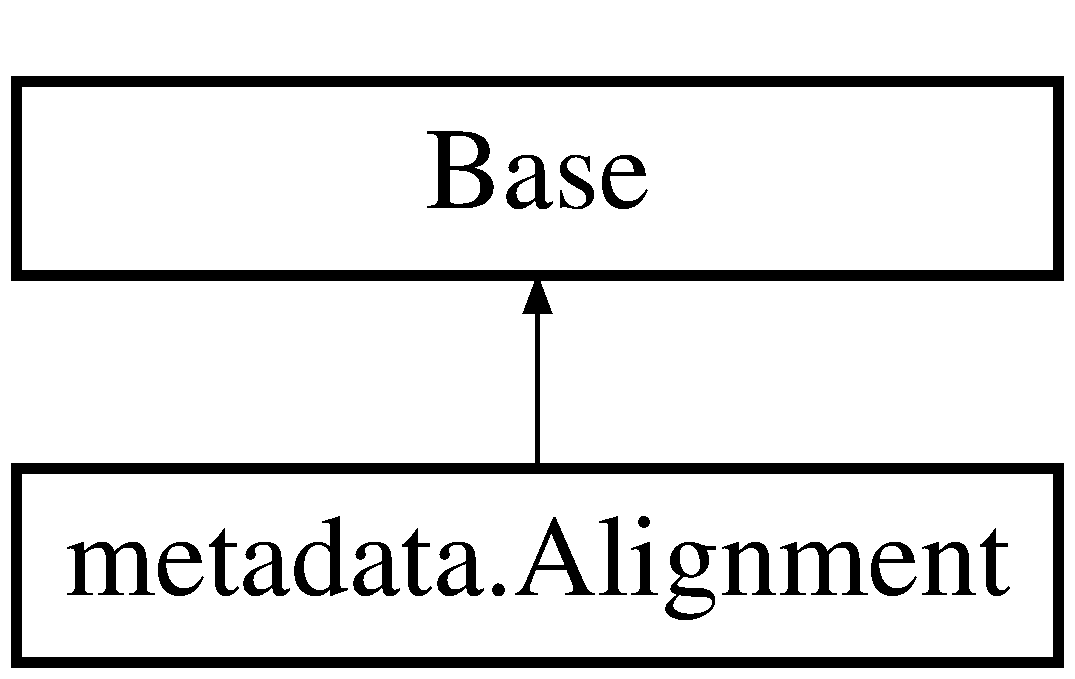
\includegraphics[height=2.000000cm]{classmetadata_1_1Alignment}
\end{center}
\end{figure}
\subsubsection*{Public Member Functions}
\begin{DoxyCompactItemize}
\item 
def \hyperlink{classmetadata_1_1Alignment_a167380dd62ad57520e11cbc05891a77f}{\-\_\-\-\_\-init\-\_\-\-\_\-}
\end{DoxyCompactItemize}
\subsubsection*{Public Attributes}
\begin{DoxyCompactItemize}
\item 
\hyperlink{classmetadata_1_1Alignment_a9e23763abf24ef8b40b62776f0d088fd}{camera\-View}
\end{DoxyCompactItemize}
\subsubsection*{Static Public Attributes}
\begin{DoxyCompactItemize}
\item 
tuple \hyperlink{classmetadata_1_1Alignment_aefc5837250a62d76466899e8720044b5}{idx} = Column(Integer, primary\-\_\-key=True)
\item 
tuple \hyperlink{classmetadata_1_1Alignment_aad17a6114e7cd9602aa7cd297cd7465e}{camera\-View\-Idx} = Column(Integer, Foreign\-Key('camera\-\_\-views.\-idx'))
\item 
tuple \hyperlink{classmetadata_1_1Alignment_a598b4395f5de4eb2ba5fb4fa4f3949da}{camera\-View} = relationship(\char`\"{}Camera\-View\char`\"{}, backref=backref('alignments', order\-\_\-by = \hyperlink{classmetadata_1_1Alignment_aefc5837250a62d76466899e8720044b5}{idx}))
\end{DoxyCompactItemize}


\subsubsection{Constructor \& Destructor Documentation}
\hypertarget{classmetadata_1_1Alignment_a167380dd62ad57520e11cbc05891a77f}{\index{metadata\-::\-Alignment@{metadata\-::\-Alignment}!\-\_\-\-\_\-init\-\_\-\-\_\-@{\-\_\-\-\_\-init\-\_\-\-\_\-}}
\index{\-\_\-\-\_\-init\-\_\-\-\_\-@{\-\_\-\-\_\-init\-\_\-\-\_\-}!metadata::Alignment@{metadata\-::\-Alignment}}
\paragraph[{\-\_\-\-\_\-init\-\_\-\-\_\-}]{\setlength{\rightskip}{0pt plus 5cm}def metadata.\-Alignment.\-\_\-\-\_\-init\-\_\-\-\_\- (
\begin{DoxyParamCaption}
\item[{}]{self, }
\item[{}]{camera\-View}
\end{DoxyParamCaption}
)}}\label{classmetadata_1_1Alignment_a167380dd62ad57520e11cbc05891a77f}


\subsubsection{Member Data Documentation}
\hypertarget{classmetadata_1_1Alignment_a598b4395f5de4eb2ba5fb4fa4f3949da}{\index{metadata\-::\-Alignment@{metadata\-::\-Alignment}!camera\-View@{camera\-View}}
\index{camera\-View@{camera\-View}!metadata::Alignment@{metadata\-::\-Alignment}}
\paragraph[{camera\-View}]{\setlength{\rightskip}{0pt plus 5cm}tuple metadata.\-Alignment.\-camera\-View = relationship(\char`\"{}Camera\-View\char`\"{}, backref=backref('alignments', order\-\_\-by = {\bf idx}))\hspace{0.3cm}{\ttfamily [static]}}}\label{classmetadata_1_1Alignment_a598b4395f5de4eb2ba5fb4fa4f3949da}
\hypertarget{classmetadata_1_1Alignment_a9e23763abf24ef8b40b62776f0d088fd}{\index{metadata\-::\-Alignment@{metadata\-::\-Alignment}!camera\-View@{camera\-View}}
\index{camera\-View@{camera\-View}!metadata::Alignment@{metadata\-::\-Alignment}}
\paragraph[{camera\-View}]{\setlength{\rightskip}{0pt plus 5cm}metadata.\-Alignment.\-camera\-View}}\label{classmetadata_1_1Alignment_a9e23763abf24ef8b40b62776f0d088fd}
\hypertarget{classmetadata_1_1Alignment_aad17a6114e7cd9602aa7cd297cd7465e}{\index{metadata\-::\-Alignment@{metadata\-::\-Alignment}!camera\-View\-Idx@{camera\-View\-Idx}}
\index{camera\-View\-Idx@{camera\-View\-Idx}!metadata::Alignment@{metadata\-::\-Alignment}}
\paragraph[{camera\-View\-Idx}]{\setlength{\rightskip}{0pt plus 5cm}tuple metadata.\-Alignment.\-camera\-View\-Idx = Column(Integer, Foreign\-Key('camera\-\_\-views.\-idx'))\hspace{0.3cm}{\ttfamily [static]}}}\label{classmetadata_1_1Alignment_aad17a6114e7cd9602aa7cd297cd7465e}
\hypertarget{classmetadata_1_1Alignment_aefc5837250a62d76466899e8720044b5}{\index{metadata\-::\-Alignment@{metadata\-::\-Alignment}!idx@{idx}}
\index{idx@{idx}!metadata::Alignment@{metadata\-::\-Alignment}}
\paragraph[{idx}]{\setlength{\rightskip}{0pt plus 5cm}tuple metadata.\-Alignment.\-idx = Column(Integer, primary\-\_\-key=True)\hspace{0.3cm}{\ttfamily [static]}}}\label{classmetadata_1_1Alignment_aefc5837250a62d76466899e8720044b5}


The documentation for this class was generated from the following file\-:\begin{DoxyCompactItemize}
\item 
python/\hyperlink{metadata_8py}{metadata.\-py}\end{DoxyCompactItemize}

\hypertarget{classCatch_1_1Detail_1_1Approx}{\subsection{Catch\-:\-:Detail\-:\-:Approx Class Reference}
\label{classCatch_1_1Detail_1_1Approx}\index{Catch\-::\-Detail\-::\-Approx@{Catch\-::\-Detail\-::\-Approx}}
}


{\ttfamily \#include $<$catch.\-hpp$>$}

\subsubsection*{Public Member Functions}
\begin{DoxyCompactItemize}
\item 
\hyperlink{classCatch_1_1Detail_1_1Approx_a1a8618ea8db08c66bd3d9fe8f74b957a}{Approx} (double value)
\item 
\hyperlink{classCatch_1_1Detail_1_1Approx_a37104584a2e20000b55700f8af92fbf2}{Approx} (const \hyperlink{classCatch_1_1Detail_1_1Approx}{Approx} \&other)
\item 
\hyperlink{classCatch_1_1Detail_1_1Approx}{Approx} \hyperlink{classCatch_1_1Detail_1_1Approx_a48c9cbc28a05dc9dc8c3973b9eae2268}{operator()} (double value)
\item 
\hyperlink{classCatch_1_1Detail_1_1Approx}{Approx} \& \hyperlink{classCatch_1_1Detail_1_1Approx_a05c50c3ad0a971fab19345b5d94979a9}{epsilon} (double new\-Epsilon)
\item 
\hyperlink{classCatch_1_1Detail_1_1Approx}{Approx} \& \hyperlink{classCatch_1_1Detail_1_1Approx_acd80f0737bf38112beacd5ca95bef113}{scale} (double new\-Scale)
\item 
std\-::string \hyperlink{classCatch_1_1Detail_1_1Approx_adeb74b73506b3f6b2ba72aea15168fbe}{to\-String} () const 
\end{DoxyCompactItemize}
\subsubsection*{Static Public Member Functions}
\begin{DoxyCompactItemize}
\item 
static \hyperlink{classCatch_1_1Detail_1_1Approx}{Approx} \hyperlink{classCatch_1_1Detail_1_1Approx_aaf86dc0ee92272ac2d9839197a07951d}{custom} ()
\end{DoxyCompactItemize}
\subsubsection*{Friends}
\begin{DoxyCompactItemize}
\item 
bool \hyperlink{classCatch_1_1Detail_1_1Approx_a18af42d25e159f300e7ed4d77c06fa09}{operator==} (double lhs, const \hyperlink{classCatch_1_1Detail_1_1Approx}{Approx} \&rhs)
\item 
bool \hyperlink{classCatch_1_1Detail_1_1Approx_ad5ee5cd12e2bcde2227272661c3ae187}{operator==} (const \hyperlink{classCatch_1_1Detail_1_1Approx}{Approx} \&lhs, double rhs)
\item 
bool \hyperlink{classCatch_1_1Detail_1_1Approx_a41f275e4477e91642fd4c997dfef3546}{operator!=} (double lhs, const \hyperlink{classCatch_1_1Detail_1_1Approx}{Approx} \&rhs)
\item 
bool \hyperlink{classCatch_1_1Detail_1_1Approx_a6828a6aec6b5b9f8b8160165aa5414a5}{operator!=} (const \hyperlink{classCatch_1_1Detail_1_1Approx}{Approx} \&lhs, double rhs)
\end{DoxyCompactItemize}


\subsubsection{Constructor \& Destructor Documentation}
\hypertarget{classCatch_1_1Detail_1_1Approx_a1a8618ea8db08c66bd3d9fe8f74b957a}{\index{Catch\-::\-Detail\-::\-Approx@{Catch\-::\-Detail\-::\-Approx}!Approx@{Approx}}
\index{Approx@{Approx}!Catch::Detail::Approx@{Catch\-::\-Detail\-::\-Approx}}
\paragraph[{Approx}]{\setlength{\rightskip}{0pt plus 5cm}Catch\-::\-Detail\-::\-Approx\-::\-Approx (
\begin{DoxyParamCaption}
\item[{double}]{value}
\end{DoxyParamCaption}
)\hspace{0.3cm}{\ttfamily [inline]}, {\ttfamily [explicit]}}}\label{classCatch_1_1Detail_1_1Approx_a1a8618ea8db08c66bd3d9fe8f74b957a}
\hypertarget{classCatch_1_1Detail_1_1Approx_a37104584a2e20000b55700f8af92fbf2}{\index{Catch\-::\-Detail\-::\-Approx@{Catch\-::\-Detail\-::\-Approx}!Approx@{Approx}}
\index{Approx@{Approx}!Catch::Detail::Approx@{Catch\-::\-Detail\-::\-Approx}}
\paragraph[{Approx}]{\setlength{\rightskip}{0pt plus 5cm}Catch\-::\-Detail\-::\-Approx\-::\-Approx (
\begin{DoxyParamCaption}
\item[{const {\bf Approx} \&}]{other}
\end{DoxyParamCaption}
)\hspace{0.3cm}{\ttfamily [inline]}}}\label{classCatch_1_1Detail_1_1Approx_a37104584a2e20000b55700f8af92fbf2}


\subsubsection{Member Function Documentation}
\hypertarget{classCatch_1_1Detail_1_1Approx_aaf86dc0ee92272ac2d9839197a07951d}{\index{Catch\-::\-Detail\-::\-Approx@{Catch\-::\-Detail\-::\-Approx}!custom@{custom}}
\index{custom@{custom}!Catch::Detail::Approx@{Catch\-::\-Detail\-::\-Approx}}
\paragraph[{custom}]{\setlength{\rightskip}{0pt plus 5cm}static {\bf Approx} Catch\-::\-Detail\-::\-Approx\-::custom (
\begin{DoxyParamCaption}
{}
\end{DoxyParamCaption}
)\hspace{0.3cm}{\ttfamily [inline]}, {\ttfamily [static]}}}\label{classCatch_1_1Detail_1_1Approx_aaf86dc0ee92272ac2d9839197a07951d}


References Approx().

\hypertarget{classCatch_1_1Detail_1_1Approx_a05c50c3ad0a971fab19345b5d94979a9}{\index{Catch\-::\-Detail\-::\-Approx@{Catch\-::\-Detail\-::\-Approx}!epsilon@{epsilon}}
\index{epsilon@{epsilon}!Catch::Detail::Approx@{Catch\-::\-Detail\-::\-Approx}}
\paragraph[{epsilon}]{\setlength{\rightskip}{0pt plus 5cm}{\bf Approx}\& Catch\-::\-Detail\-::\-Approx\-::epsilon (
\begin{DoxyParamCaption}
\item[{double}]{new\-Epsilon}
\end{DoxyParamCaption}
)\hspace{0.3cm}{\ttfamily [inline]}}}\label{classCatch_1_1Detail_1_1Approx_a05c50c3ad0a971fab19345b5d94979a9}
\hypertarget{classCatch_1_1Detail_1_1Approx_a48c9cbc28a05dc9dc8c3973b9eae2268}{\index{Catch\-::\-Detail\-::\-Approx@{Catch\-::\-Detail\-::\-Approx}!operator()@{operator()}}
\index{operator()@{operator()}!Catch::Detail::Approx@{Catch\-::\-Detail\-::\-Approx}}
\paragraph[{operator()}]{\setlength{\rightskip}{0pt plus 5cm}{\bf Approx} Catch\-::\-Detail\-::\-Approx\-::operator() (
\begin{DoxyParamCaption}
\item[{double}]{value}
\end{DoxyParamCaption}
)\hspace{0.3cm}{\ttfamily [inline]}}}\label{classCatch_1_1Detail_1_1Approx_a48c9cbc28a05dc9dc8c3973b9eae2268}


References epsilon(), and scale().

\hypertarget{classCatch_1_1Detail_1_1Approx_acd80f0737bf38112beacd5ca95bef113}{\index{Catch\-::\-Detail\-::\-Approx@{Catch\-::\-Detail\-::\-Approx}!scale@{scale}}
\index{scale@{scale}!Catch::Detail::Approx@{Catch\-::\-Detail\-::\-Approx}}
\paragraph[{scale}]{\setlength{\rightskip}{0pt plus 5cm}{\bf Approx}\& Catch\-::\-Detail\-::\-Approx\-::scale (
\begin{DoxyParamCaption}
\item[{double}]{new\-Scale}
\end{DoxyParamCaption}
)\hspace{0.3cm}{\ttfamily [inline]}}}\label{classCatch_1_1Detail_1_1Approx_acd80f0737bf38112beacd5ca95bef113}
\hypertarget{classCatch_1_1Detail_1_1Approx_adeb74b73506b3f6b2ba72aea15168fbe}{\index{Catch\-::\-Detail\-::\-Approx@{Catch\-::\-Detail\-::\-Approx}!to\-String@{to\-String}}
\index{to\-String@{to\-String}!Catch::Detail::Approx@{Catch\-::\-Detail\-::\-Approx}}
\paragraph[{to\-String}]{\setlength{\rightskip}{0pt plus 5cm}std\-::string Catch\-::\-Detail\-::\-Approx\-::to\-String (
\begin{DoxyParamCaption}
{}
\end{DoxyParamCaption}
) const\hspace{0.3cm}{\ttfamily [inline]}}}\label{classCatch_1_1Detail_1_1Approx_adeb74b73506b3f6b2ba72aea15168fbe}


\subsubsection{Friends And Related Function Documentation}
\hypertarget{classCatch_1_1Detail_1_1Approx_a41f275e4477e91642fd4c997dfef3546}{\index{Catch\-::\-Detail\-::\-Approx@{Catch\-::\-Detail\-::\-Approx}!operator!=@{operator!=}}
\index{operator!=@{operator!=}!Catch::Detail::Approx@{Catch\-::\-Detail\-::\-Approx}}
\paragraph[{operator!=}]{\setlength{\rightskip}{0pt plus 5cm}bool operator!= (
\begin{DoxyParamCaption}
\item[{double}]{lhs, }
\item[{const {\bf Approx} \&}]{rhs}
\end{DoxyParamCaption}
)\hspace{0.3cm}{\ttfamily [friend]}}}\label{classCatch_1_1Detail_1_1Approx_a41f275e4477e91642fd4c997dfef3546}
\hypertarget{classCatch_1_1Detail_1_1Approx_a6828a6aec6b5b9f8b8160165aa5414a5}{\index{Catch\-::\-Detail\-::\-Approx@{Catch\-::\-Detail\-::\-Approx}!operator!=@{operator!=}}
\index{operator!=@{operator!=}!Catch::Detail::Approx@{Catch\-::\-Detail\-::\-Approx}}
\paragraph[{operator!=}]{\setlength{\rightskip}{0pt plus 5cm}bool operator!= (
\begin{DoxyParamCaption}
\item[{const {\bf Approx} \&}]{lhs, }
\item[{double}]{rhs}
\end{DoxyParamCaption}
)\hspace{0.3cm}{\ttfamily [friend]}}}\label{classCatch_1_1Detail_1_1Approx_a6828a6aec6b5b9f8b8160165aa5414a5}
\hypertarget{classCatch_1_1Detail_1_1Approx_a18af42d25e159f300e7ed4d77c06fa09}{\index{Catch\-::\-Detail\-::\-Approx@{Catch\-::\-Detail\-::\-Approx}!operator==@{operator==}}
\index{operator==@{operator==}!Catch::Detail::Approx@{Catch\-::\-Detail\-::\-Approx}}
\paragraph[{operator==}]{\setlength{\rightskip}{0pt plus 5cm}bool operator== (
\begin{DoxyParamCaption}
\item[{double}]{lhs, }
\item[{const {\bf Approx} \&}]{rhs}
\end{DoxyParamCaption}
)\hspace{0.3cm}{\ttfamily [friend]}}}\label{classCatch_1_1Detail_1_1Approx_a18af42d25e159f300e7ed4d77c06fa09}
\hypertarget{classCatch_1_1Detail_1_1Approx_ad5ee5cd12e2bcde2227272661c3ae187}{\index{Catch\-::\-Detail\-::\-Approx@{Catch\-::\-Detail\-::\-Approx}!operator==@{operator==}}
\index{operator==@{operator==}!Catch::Detail::Approx@{Catch\-::\-Detail\-::\-Approx}}
\paragraph[{operator==}]{\setlength{\rightskip}{0pt plus 5cm}bool operator== (
\begin{DoxyParamCaption}
\item[{const {\bf Approx} \&}]{lhs, }
\item[{double}]{rhs}
\end{DoxyParamCaption}
)\hspace{0.3cm}{\ttfamily [friend]}}}\label{classCatch_1_1Detail_1_1Approx_ad5ee5cd12e2bcde2227272661c3ae187}


The documentation for this class was generated from the following file\-:\begin{DoxyCompactItemize}
\item 
include/\hyperlink{catch_8hpp}{catch.\-hpp}\end{DoxyCompactItemize}

\hypertarget{structCatch_1_1AutoReg}{\subsection{Catch\-:\-:Auto\-Reg Struct Reference}
\label{structCatch_1_1AutoReg}\index{Catch\-::\-Auto\-Reg@{Catch\-::\-Auto\-Reg}}
}


{\ttfamily \#include $<$catch.\-hpp$>$}

\subsubsection*{Public Member Functions}
\begin{DoxyCompactItemize}
\item 
\hyperlink{structCatch_1_1AutoReg_a08074c82a7bda1fdbbe80e85e10f4c59}{Auto\-Reg} (\hyperlink{namespaceCatch_a768da872b9033e4c71c6f316393d35db}{Test\-Function} function, const char $\ast$name, const char $\ast$description, const \hyperlink{structCatch_1_1SourceLineInfo}{Source\-Line\-Info} \&line\-Info)
\item 
{\footnotesize template$<$typename C $>$ }\\\hyperlink{structCatch_1_1AutoReg_a731f720d0b63c323f6e8f4f82fbdd22b}{Auto\-Reg} (void(C\-::$\ast$method)(), const char $\ast$name, const char $\ast$description, const \hyperlink{structCatch_1_1SourceLineInfo}{Source\-Line\-Info} \&line\-Info)
\item 
void \hyperlink{structCatch_1_1AutoReg_ac4123f648f75d462a4e68ad291799cf2}{register\-Test\-Case} (\hyperlink{structCatch_1_1ITestCase}{I\-Test\-Case} $\ast$test\-Case, const char $\ast$name, const char $\ast$description, const \hyperlink{structCatch_1_1SourceLineInfo}{Source\-Line\-Info} \&line\-Info)
\item 
\hyperlink{structCatch_1_1AutoReg_a3cdb53f1e5ff115310f3372bebe198f1}{$\sim$\-Auto\-Reg} ()
\end{DoxyCompactItemize}


\subsubsection{Constructor \& Destructor Documentation}
\hypertarget{structCatch_1_1AutoReg_a08074c82a7bda1fdbbe80e85e10f4c59}{\index{Catch\-::\-Auto\-Reg@{Catch\-::\-Auto\-Reg}!Auto\-Reg@{Auto\-Reg}}
\index{Auto\-Reg@{Auto\-Reg}!Catch::AutoReg@{Catch\-::\-Auto\-Reg}}
\paragraph[{Auto\-Reg}]{\setlength{\rightskip}{0pt plus 5cm}Catch\-::\-Auto\-Reg\-::\-Auto\-Reg (
\begin{DoxyParamCaption}
\item[{{\bf Test\-Function}}]{function, }
\item[{const char $\ast$}]{name, }
\item[{const char $\ast$}]{description, }
\item[{const {\bf Source\-Line\-Info} \&}]{line\-Info}
\end{DoxyParamCaption}
)}}\label{structCatch_1_1AutoReg_a08074c82a7bda1fdbbe80e85e10f4c59}
\hypertarget{structCatch_1_1AutoReg_a731f720d0b63c323f6e8f4f82fbdd22b}{\index{Catch\-::\-Auto\-Reg@{Catch\-::\-Auto\-Reg}!Auto\-Reg@{Auto\-Reg}}
\index{Auto\-Reg@{Auto\-Reg}!Catch::AutoReg@{Catch\-::\-Auto\-Reg}}
\paragraph[{Auto\-Reg}]{\setlength{\rightskip}{0pt plus 5cm}template$<$typename C $>$ Catch\-::\-Auto\-Reg\-::\-Auto\-Reg (
\begin{DoxyParamCaption}
\item[{void(C\-::$\ast$)()}]{method, }
\item[{const char $\ast$}]{name, }
\item[{const char $\ast$}]{description, }
\item[{const {\bf Source\-Line\-Info} \&}]{line\-Info}
\end{DoxyParamCaption}
)\hspace{0.3cm}{\ttfamily [inline]}}}\label{structCatch_1_1AutoReg_a731f720d0b63c323f6e8f4f82fbdd22b}


References register\-Test\-Case().

\hypertarget{structCatch_1_1AutoReg_a3cdb53f1e5ff115310f3372bebe198f1}{\index{Catch\-::\-Auto\-Reg@{Catch\-::\-Auto\-Reg}!$\sim$\-Auto\-Reg@{$\sim$\-Auto\-Reg}}
\index{$\sim$\-Auto\-Reg@{$\sim$\-Auto\-Reg}!Catch::AutoReg@{Catch\-::\-Auto\-Reg}}
\paragraph[{$\sim$\-Auto\-Reg}]{\setlength{\rightskip}{0pt plus 5cm}Catch\-::\-Auto\-Reg\-::$\sim$\-Auto\-Reg (
\begin{DoxyParamCaption}
{}
\end{DoxyParamCaption}
)}}\label{structCatch_1_1AutoReg_a3cdb53f1e5ff115310f3372bebe198f1}


\subsubsection{Member Function Documentation}
\hypertarget{structCatch_1_1AutoReg_ac4123f648f75d462a4e68ad291799cf2}{\index{Catch\-::\-Auto\-Reg@{Catch\-::\-Auto\-Reg}!register\-Test\-Case@{register\-Test\-Case}}
\index{register\-Test\-Case@{register\-Test\-Case}!Catch::AutoReg@{Catch\-::\-Auto\-Reg}}
\paragraph[{register\-Test\-Case}]{\setlength{\rightskip}{0pt plus 5cm}void Catch\-::\-Auto\-Reg\-::register\-Test\-Case (
\begin{DoxyParamCaption}
\item[{{\bf I\-Test\-Case} $\ast$}]{test\-Case, }
\item[{const char $\ast$}]{name, }
\item[{const char $\ast$}]{description, }
\item[{const {\bf Source\-Line\-Info} \&}]{line\-Info}
\end{DoxyParamCaption}
)}}\label{structCatch_1_1AutoReg_ac4123f648f75d462a4e68ad291799cf2}


The documentation for this struct was generated from the following file\-:\begin{DoxyCompactItemize}
\item 
include/\hyperlink{catch_8hpp}{catch.\-hpp}\end{DoxyCompactItemize}

\hypertarget{classmoving_1_1BBAnnotation}{\subsection{moving.\-B\-B\-Annotation Class Reference}
\label{classmoving_1_1BBAnnotation}\index{moving.\-B\-B\-Annotation@{moving.\-B\-B\-Annotation}}
}
Inheritance diagram for moving.\-B\-B\-Annotation\-:\begin{figure}[H]
\begin{center}
\leavevmode
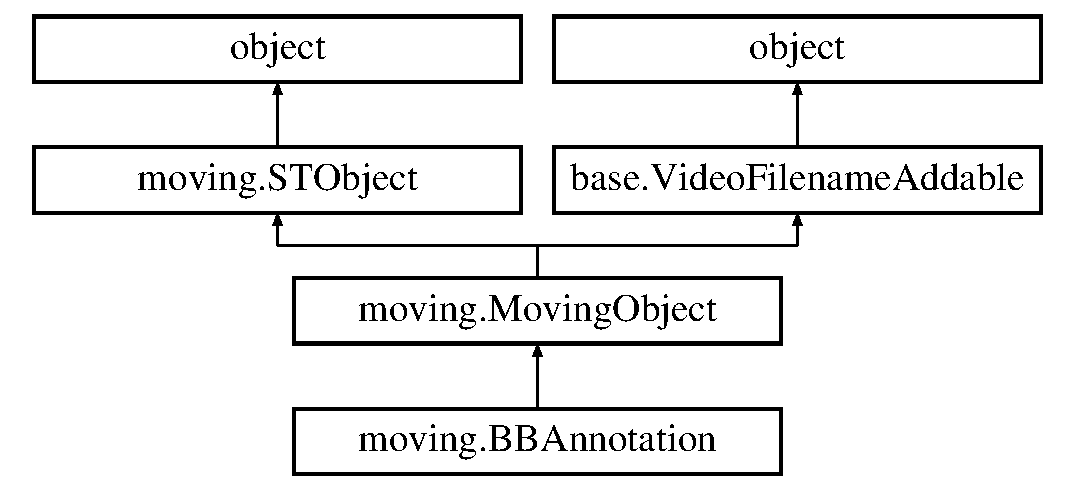
\includegraphics[height=4.000000cm]{classmoving_1_1BBAnnotation}
\end{center}
\end{figure}
\subsubsection*{Public Member Functions}
\begin{DoxyCompactItemize}
\item 
def \hyperlink{classmoving_1_1BBAnnotation_a44f6380b3b0377241c4768c1496afb44}{\-\_\-\-\_\-init\-\_\-\-\_\-}
\item 
def \hyperlink{classmoving_1_1BBAnnotation_aec41e86c251788e5edeb62849fd947f2}{compute\-Centroid\-Trajectory}
\item 
def \hyperlink{classmoving_1_1BBAnnotation_a129e3755fa6eb0ee2d230a21028e924e}{matches}
\end{DoxyCompactItemize}
\subsubsection*{Public Attributes}
\begin{DoxyCompactItemize}
\item 
\hyperlink{classmoving_1_1BBAnnotation_a5ccafeea40b41e138d54c6cbcf11ae1f}{top\-Left\-Positions}
\item 
\hyperlink{classmoving_1_1BBAnnotation_abc54d8997043b819f76dced20c48b94d}{bottom\-Right\-Positions}
\item 
\hyperlink{classmoving_1_1BBAnnotation_a0f4ee909fb7d67b60f5abc94943207c5}{positions}
\end{DoxyCompactItemize}
\subsubsection*{Additional Inherited Members}


\subsubsection{Detailed Description}
\begin{DoxyVerb}Class for a series of ground truth annotations using bounding boxes
Its center is the center of the containing shape

By default in image space
\end{DoxyVerb}
 

\subsubsection{Constructor \& Destructor Documentation}
\hypertarget{classmoving_1_1BBAnnotation_a44f6380b3b0377241c4768c1496afb44}{\index{moving\-::\-B\-B\-Annotation@{moving\-::\-B\-B\-Annotation}!\-\_\-\-\_\-init\-\_\-\-\_\-@{\-\_\-\-\_\-init\-\_\-\-\_\-}}
\index{\-\_\-\-\_\-init\-\_\-\-\_\-@{\-\_\-\-\_\-init\-\_\-\-\_\-}!moving::BBAnnotation@{moving\-::\-B\-B\-Annotation}}
\paragraph[{\-\_\-\-\_\-init\-\_\-\-\_\-}]{\setlength{\rightskip}{0pt plus 5cm}def moving.\-B\-B\-Annotation.\-\_\-\-\_\-init\-\_\-\-\_\- (
\begin{DoxyParamCaption}
\item[{}]{self, }
\item[{}]{num = {\ttfamily None}, }
\item[{}]{time\-Interval = {\ttfamily None}, }
\item[{}]{top\-Left\-Positions = {\ttfamily None}, }
\item[{}]{bottom\-Right\-Positions = {\ttfamily None}, }
\item[{}]{user\-Type = {\ttfamily {\bf user\-Type2\-Num}\mbox{[}'unknown'\mbox{]}}}
\end{DoxyParamCaption}
)}}\label{classmoving_1_1BBAnnotation_a44f6380b3b0377241c4768c1496afb44}


\subsubsection{Member Function Documentation}
\hypertarget{classmoving_1_1BBAnnotation_aec41e86c251788e5edeb62849fd947f2}{\index{moving\-::\-B\-B\-Annotation@{moving\-::\-B\-B\-Annotation}!compute\-Centroid\-Trajectory@{compute\-Centroid\-Trajectory}}
\index{compute\-Centroid\-Trajectory@{compute\-Centroid\-Trajectory}!moving::BBAnnotation@{moving\-::\-B\-B\-Annotation}}
\paragraph[{compute\-Centroid\-Trajectory}]{\setlength{\rightskip}{0pt plus 5cm}def moving.\-B\-B\-Annotation.\-compute\-Centroid\-Trajectory (
\begin{DoxyParamCaption}
\item[{}]{self, }
\item[{}]{homography = {\ttfamily None}}
\end{DoxyParamCaption}
)}}\label{classmoving_1_1BBAnnotation_aec41e86c251788e5edeb62849fd947f2}
\hypertarget{classmoving_1_1BBAnnotation_a129e3755fa6eb0ee2d230a21028e924e}{\index{moving\-::\-B\-B\-Annotation@{moving\-::\-B\-B\-Annotation}!matches@{matches}}
\index{matches@{matches}!moving::BBAnnotation@{moving\-::\-B\-B\-Annotation}}
\paragraph[{matches}]{\setlength{\rightskip}{0pt plus 5cm}def moving.\-B\-B\-Annotation.\-matches (
\begin{DoxyParamCaption}
\item[{}]{self, }
\item[{}]{obj, }
\item[{}]{instant, }
\item[{}]{matching\-Distance}
\end{DoxyParamCaption}
)}}\label{classmoving_1_1BBAnnotation_a129e3755fa6eb0ee2d230a21028e924e}
\begin{DoxyVerb}Indicates if the annotation matches obj (MovingObject)
with threshold matchingDistance
Returns distance if below matchingDistance, matchingDistance+1 otherwise
(returns an actual value, otherwise munkres does not terminate)\end{DoxyVerb}
 

References moving.\-Moving\-Object.\-get\-Position\-At\-Instant().



\subsubsection{Member Data Documentation}
\hypertarget{classmoving_1_1BBAnnotation_abc54d8997043b819f76dced20c48b94d}{\index{moving\-::\-B\-B\-Annotation@{moving\-::\-B\-B\-Annotation}!bottom\-Right\-Positions@{bottom\-Right\-Positions}}
\index{bottom\-Right\-Positions@{bottom\-Right\-Positions}!moving::BBAnnotation@{moving\-::\-B\-B\-Annotation}}
\paragraph[{bottom\-Right\-Positions}]{\setlength{\rightskip}{0pt plus 5cm}moving.\-B\-B\-Annotation.\-bottom\-Right\-Positions}}\label{classmoving_1_1BBAnnotation_abc54d8997043b819f76dced20c48b94d}
\hypertarget{classmoving_1_1BBAnnotation_a0f4ee909fb7d67b60f5abc94943207c5}{\index{moving\-::\-B\-B\-Annotation@{moving\-::\-B\-B\-Annotation}!positions@{positions}}
\index{positions@{positions}!moving::BBAnnotation@{moving\-::\-B\-B\-Annotation}}
\paragraph[{positions}]{\setlength{\rightskip}{0pt plus 5cm}moving.\-B\-B\-Annotation.\-positions}}\label{classmoving_1_1BBAnnotation_a0f4ee909fb7d67b60f5abc94943207c5}
\hypertarget{classmoving_1_1BBAnnotation_a5ccafeea40b41e138d54c6cbcf11ae1f}{\index{moving\-::\-B\-B\-Annotation@{moving\-::\-B\-B\-Annotation}!top\-Left\-Positions@{top\-Left\-Positions}}
\index{top\-Left\-Positions@{top\-Left\-Positions}!moving::BBAnnotation@{moving\-::\-B\-B\-Annotation}}
\paragraph[{top\-Left\-Positions}]{\setlength{\rightskip}{0pt plus 5cm}moving.\-B\-B\-Annotation.\-top\-Left\-Positions}}\label{classmoving_1_1BBAnnotation_a5ccafeea40b41e138d54c6cbcf11ae1f}


The documentation for this class was generated from the following file\-:\begin{DoxyCompactItemize}
\item 
python/\hyperlink{moving_8py}{moving.\-py}\end{DoxyCompactItemize}

\hypertarget{classCatch_1_1BetweenGenerator}{\subsection{Catch\-:\-:Between\-Generator$<$ T $>$ Class Template Reference}
\label{classCatch_1_1BetweenGenerator}\index{Catch\-::\-Between\-Generator$<$ T $>$@{Catch\-::\-Between\-Generator$<$ T $>$}}
}


{\ttfamily \#include $<$catch.\-hpp$>$}

Inheritance diagram for Catch\-:\-:Between\-Generator$<$ T $>$\-:\begin{figure}[H]
\begin{center}
\leavevmode
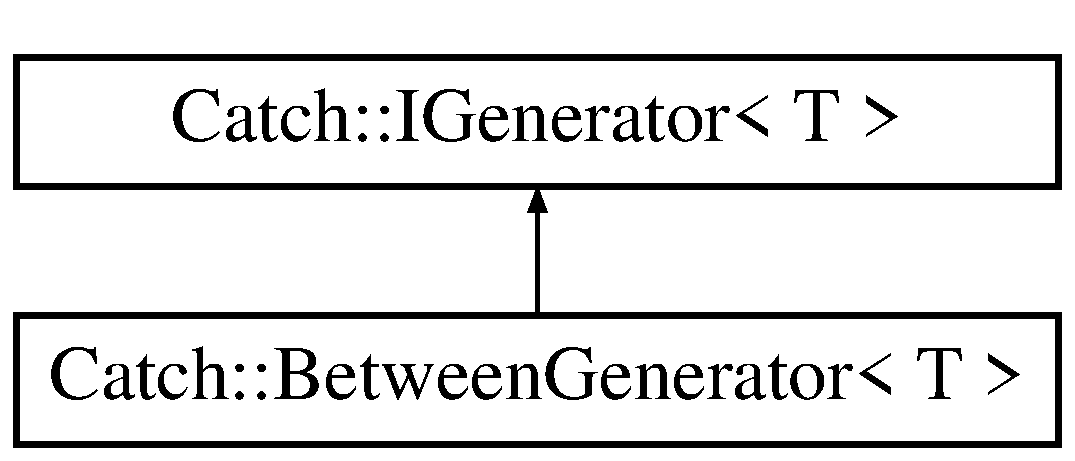
\includegraphics[height=2.000000cm]{classCatch_1_1BetweenGenerator}
\end{center}
\end{figure}
\subsubsection*{Public Member Functions}
\begin{DoxyCompactItemize}
\item 
\hyperlink{classCatch_1_1BetweenGenerator_a835a057d691ae37caef660624099b51c}{Between\-Generator} (T from, T to)
\item 
virtual T \hyperlink{classCatch_1_1BetweenGenerator_af83575d62cc727ca995446cff4d6c26c}{get\-Value} (std\-::size\-\_\-t index) const 
\item 
virtual std\-::size\-\_\-t \hyperlink{classCatch_1_1BetweenGenerator_aa53a04a259e796ba2b5adabed79474b5}{size} () const 
\end{DoxyCompactItemize}


\subsubsection{Constructor \& Destructor Documentation}
\hypertarget{classCatch_1_1BetweenGenerator_a835a057d691ae37caef660624099b51c}{\index{Catch\-::\-Between\-Generator@{Catch\-::\-Between\-Generator}!Between\-Generator@{Between\-Generator}}
\index{Between\-Generator@{Between\-Generator}!Catch::BetweenGenerator@{Catch\-::\-Between\-Generator}}
\paragraph[{Between\-Generator}]{\setlength{\rightskip}{0pt plus 5cm}template$<$typename T $>$ {\bf Catch\-::\-Between\-Generator}$<$ T $>$\-::{\bf Between\-Generator} (
\begin{DoxyParamCaption}
\item[{T}]{from, }
\item[{T}]{to}
\end{DoxyParamCaption}
)\hspace{0.3cm}{\ttfamily [inline]}}}\label{classCatch_1_1BetweenGenerator_a835a057d691ae37caef660624099b51c}


\subsubsection{Member Function Documentation}
\hypertarget{classCatch_1_1BetweenGenerator_af83575d62cc727ca995446cff4d6c26c}{\index{Catch\-::\-Between\-Generator@{Catch\-::\-Between\-Generator}!get\-Value@{get\-Value}}
\index{get\-Value@{get\-Value}!Catch::BetweenGenerator@{Catch\-::\-Between\-Generator}}
\paragraph[{get\-Value}]{\setlength{\rightskip}{0pt plus 5cm}template$<$typename T $>$ virtual T {\bf Catch\-::\-Between\-Generator}$<$ T $>$\-::get\-Value (
\begin{DoxyParamCaption}
\item[{std\-::size\-\_\-t}]{index}
\end{DoxyParamCaption}
) const\hspace{0.3cm}{\ttfamily [inline]}, {\ttfamily [virtual]}}}\label{classCatch_1_1BetweenGenerator_af83575d62cc727ca995446cff4d6c26c}


Implements \hyperlink{structCatch_1_1IGenerator_ad69e937cb66dba3ed9429c42abf4fce3}{Catch\-::\-I\-Generator$<$ T $>$}.

\hypertarget{classCatch_1_1BetweenGenerator_aa53a04a259e796ba2b5adabed79474b5}{\index{Catch\-::\-Between\-Generator@{Catch\-::\-Between\-Generator}!size@{size}}
\index{size@{size}!Catch::BetweenGenerator@{Catch\-::\-Between\-Generator}}
\paragraph[{size}]{\setlength{\rightskip}{0pt plus 5cm}template$<$typename T $>$ virtual std\-::size\-\_\-t {\bf Catch\-::\-Between\-Generator}$<$ T $>$\-::size (
\begin{DoxyParamCaption}
{}
\end{DoxyParamCaption}
) const\hspace{0.3cm}{\ttfamily [inline]}, {\ttfamily [virtual]}}}\label{classCatch_1_1BetweenGenerator_aa53a04a259e796ba2b5adabed79474b5}


Implements \hyperlink{structCatch_1_1IGenerator_a2e317253b03e838b6065ce69719a198e}{Catch\-::\-I\-Generator$<$ T $>$}.



The documentation for this class was generated from the following file\-:\begin{DoxyCompactItemize}
\item 
include/\hyperlink{catch_8hpp}{catch.\-hpp}\end{DoxyCompactItemize}

\hypertarget{classmetadata_1_1CameraView}{\subsection{metadata.\-Camera\-View Class Reference}
\label{classmetadata_1_1CameraView}\index{metadata.\-Camera\-View@{metadata.\-Camera\-View}}
}
Inheritance diagram for metadata.\-Camera\-View\-:\begin{figure}[H]
\begin{center}
\leavevmode
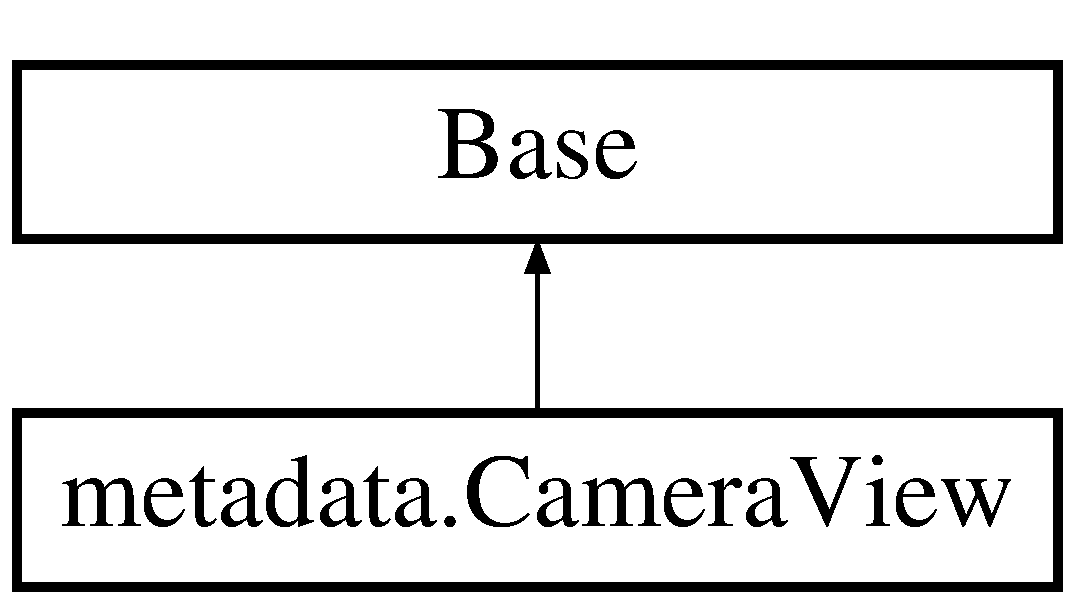
\includegraphics[height=2.000000cm]{classmetadata_1_1CameraView}
\end{center}
\end{figure}
\subsubsection*{Public Member Functions}
\begin{DoxyCompactItemize}
\item 
def \hyperlink{classmetadata_1_1CameraView_a3ce0b1e857b66e1899f8686db1f657b2}{\-\_\-\-\_\-init\-\_\-\-\_\-}
\item 
def \hyperlink{classmetadata_1_1CameraView_a18b16e48934d1157147e3bf53eac61d9}{get\-Homography\-Filename}
\end{DoxyCompactItemize}
\subsubsection*{Public Attributes}
\begin{DoxyCompactItemize}
\item 
\hyperlink{classmetadata_1_1CameraView_ae550f1d2d9dc3af754cf49370140cff0}{frame\-Rate}
\item 
\hyperlink{classmetadata_1_1CameraView_add6210fa2e81de03889b667218b5382a}{homography\-Filename}
\item 
\hyperlink{classmetadata_1_1CameraView_ade3d4831d427a621900ced9ffef79a08}{site}
\item 
\hyperlink{classmetadata_1_1CameraView_aa3cd42c9abe6e0dbb3e1ea54d1767f41}{configuration\-Filename}
\end{DoxyCompactItemize}
\subsubsection*{Static Public Attributes}
\begin{DoxyCompactItemize}
\item 
tuple \hyperlink{classmetadata_1_1CameraView_a735226fd4eb9bb825e05d377758f0814}{idx} = Column(Integer, primary\-\_\-key=True)
\item 
tuple \hyperlink{classmetadata_1_1CameraView_a2753cc5696ea9037670e0cb7561d37ed}{frame\-Rate} = Column(Float)
\item 
tuple \hyperlink{classmetadata_1_1CameraView_aac6aa3fbf236cd41e401cce74294b2b2}{homography\-Filename} = Column(String)
\item 
tuple \hyperlink{classmetadata_1_1CameraView_a39ad13a88908bf2bb645de4aded8a1ab}{camera\-Calibration\-Filename} = Column(String)
\item 
tuple \hyperlink{classmetadata_1_1CameraView_a0f596684a5898f249135bb6b280e74e5}{site\-Idx} = Column(Integer, Foreign\-Key('sites.\-idx'))
\item 
tuple \hyperlink{classmetadata_1_1CameraView_a5f2ce2e910ecc8b06dc88879cebb45ac}{homography\-Distance\-Unit} = Column(String, default = 'm')
\item 
tuple \hyperlink{classmetadata_1_1CameraView_ac9b4e0047cdcd38102fa83cfdec0f800}{configuration\-Filename} = Column(String)
\item 
tuple \hyperlink{classmetadata_1_1CameraView_acb7a348380b63ceff7a34df0a605e9d7}{site} = relationship(\char`\"{}Site\char`\"{}, backref=backref('camera\-\_\-views', order\-\_\-by = \hyperlink{classmetadata_1_1CameraView_a735226fd4eb9bb825e05d377758f0814}{idx}))
\end{DoxyCompactItemize}


\subsubsection{Constructor \& Destructor Documentation}
\hypertarget{classmetadata_1_1CameraView_a3ce0b1e857b66e1899f8686db1f657b2}{\index{metadata\-::\-Camera\-View@{metadata\-::\-Camera\-View}!\-\_\-\-\_\-init\-\_\-\-\_\-@{\-\_\-\-\_\-init\-\_\-\-\_\-}}
\index{\-\_\-\-\_\-init\-\_\-\-\_\-@{\-\_\-\-\_\-init\-\_\-\-\_\-}!metadata::CameraView@{metadata\-::\-Camera\-View}}
\paragraph[{\-\_\-\-\_\-init\-\_\-\-\_\-}]{\setlength{\rightskip}{0pt plus 5cm}def metadata.\-Camera\-View.\-\_\-\-\_\-init\-\_\-\-\_\- (
\begin{DoxyParamCaption}
\item[{}]{self, }
\item[{}]{frame\-Rate, }
\item[{}]{homography\-Filename, }
\item[{}]{camera\-Calibration\-Filename, }
\item[{}]{site, }
\item[{}]{configuration\-Filename}
\end{DoxyParamCaption}
)}}\label{classmetadata_1_1CameraView_a3ce0b1e857b66e1899f8686db1f657b2}


\subsubsection{Member Function Documentation}
\hypertarget{classmetadata_1_1CameraView_a18b16e48934d1157147e3bf53eac61d9}{\index{metadata\-::\-Camera\-View@{metadata\-::\-Camera\-View}!get\-Homography\-Filename@{get\-Homography\-Filename}}
\index{get\-Homography\-Filename@{get\-Homography\-Filename}!metadata::CameraView@{metadata\-::\-Camera\-View}}
\paragraph[{get\-Homography\-Filename}]{\setlength{\rightskip}{0pt plus 5cm}def metadata.\-Camera\-View.\-get\-Homography\-Filename (
\begin{DoxyParamCaption}
\item[{}]{self, }
\item[{}]{relative\-To\-Site\-Filename = {\ttfamily True}}
\end{DoxyParamCaption}
)}}\label{classmetadata_1_1CameraView_a18b16e48934d1157147e3bf53eac61d9}


References K\-L\-T\-Feature\-Tracking\-Parameters.\-homography\-Filename, and metadata.\-Camera\-View.\-homography\-Filename.



\subsubsection{Member Data Documentation}
\hypertarget{classmetadata_1_1CameraView_a39ad13a88908bf2bb645de4aded8a1ab}{\index{metadata\-::\-Camera\-View@{metadata\-::\-Camera\-View}!camera\-Calibration\-Filename@{camera\-Calibration\-Filename}}
\index{camera\-Calibration\-Filename@{camera\-Calibration\-Filename}!metadata::CameraView@{metadata\-::\-Camera\-View}}
\paragraph[{camera\-Calibration\-Filename}]{\setlength{\rightskip}{0pt plus 5cm}tuple metadata.\-Camera\-View.\-camera\-Calibration\-Filename = Column(String)\hspace{0.3cm}{\ttfamily [static]}}}\label{classmetadata_1_1CameraView_a39ad13a88908bf2bb645de4aded8a1ab}
\hypertarget{classmetadata_1_1CameraView_ac9b4e0047cdcd38102fa83cfdec0f800}{\index{metadata\-::\-Camera\-View@{metadata\-::\-Camera\-View}!configuration\-Filename@{configuration\-Filename}}
\index{configuration\-Filename@{configuration\-Filename}!metadata::CameraView@{metadata\-::\-Camera\-View}}
\paragraph[{configuration\-Filename}]{\setlength{\rightskip}{0pt plus 5cm}tuple metadata.\-Camera\-View.\-configuration\-Filename = Column(String)\hspace{0.3cm}{\ttfamily [static]}}}\label{classmetadata_1_1CameraView_ac9b4e0047cdcd38102fa83cfdec0f800}
\hypertarget{classmetadata_1_1CameraView_aa3cd42c9abe6e0dbb3e1ea54d1767f41}{\index{metadata\-::\-Camera\-View@{metadata\-::\-Camera\-View}!configuration\-Filename@{configuration\-Filename}}
\index{configuration\-Filename@{configuration\-Filename}!metadata::CameraView@{metadata\-::\-Camera\-View}}
\paragraph[{configuration\-Filename}]{\setlength{\rightskip}{0pt plus 5cm}metadata.\-Camera\-View.\-configuration\-Filename}}\label{classmetadata_1_1CameraView_aa3cd42c9abe6e0dbb3e1ea54d1767f41}
\hypertarget{classmetadata_1_1CameraView_a2753cc5696ea9037670e0cb7561d37ed}{\index{metadata\-::\-Camera\-View@{metadata\-::\-Camera\-View}!frame\-Rate@{frame\-Rate}}
\index{frame\-Rate@{frame\-Rate}!metadata::CameraView@{metadata\-::\-Camera\-View}}
\paragraph[{frame\-Rate}]{\setlength{\rightskip}{0pt plus 5cm}tuple metadata.\-Camera\-View.\-frame\-Rate = Column(Float)\hspace{0.3cm}{\ttfamily [static]}}}\label{classmetadata_1_1CameraView_a2753cc5696ea9037670e0cb7561d37ed}
\hypertarget{classmetadata_1_1CameraView_ae550f1d2d9dc3af754cf49370140cff0}{\index{metadata\-::\-Camera\-View@{metadata\-::\-Camera\-View}!frame\-Rate@{frame\-Rate}}
\index{frame\-Rate@{frame\-Rate}!metadata::CameraView@{metadata\-::\-Camera\-View}}
\paragraph[{frame\-Rate}]{\setlength{\rightskip}{0pt plus 5cm}metadata.\-Camera\-View.\-frame\-Rate}}\label{classmetadata_1_1CameraView_ae550f1d2d9dc3af754cf49370140cff0}
\hypertarget{classmetadata_1_1CameraView_a5f2ce2e910ecc8b06dc88879cebb45ac}{\index{metadata\-::\-Camera\-View@{metadata\-::\-Camera\-View}!homography\-Distance\-Unit@{homography\-Distance\-Unit}}
\index{homography\-Distance\-Unit@{homography\-Distance\-Unit}!metadata::CameraView@{metadata\-::\-Camera\-View}}
\paragraph[{homography\-Distance\-Unit}]{\setlength{\rightskip}{0pt plus 5cm}tuple metadata.\-Camera\-View.\-homography\-Distance\-Unit = Column(String, default = 'm')\hspace{0.3cm}{\ttfamily [static]}}}\label{classmetadata_1_1CameraView_a5f2ce2e910ecc8b06dc88879cebb45ac}
\hypertarget{classmetadata_1_1CameraView_aac6aa3fbf236cd41e401cce74294b2b2}{\index{metadata\-::\-Camera\-View@{metadata\-::\-Camera\-View}!homography\-Filename@{homography\-Filename}}
\index{homography\-Filename@{homography\-Filename}!metadata::CameraView@{metadata\-::\-Camera\-View}}
\paragraph[{homography\-Filename}]{\setlength{\rightskip}{0pt plus 5cm}tuple metadata.\-Camera\-View.\-homography\-Filename = Column(String)\hspace{0.3cm}{\ttfamily [static]}}}\label{classmetadata_1_1CameraView_aac6aa3fbf236cd41e401cce74294b2b2}
\hypertarget{classmetadata_1_1CameraView_add6210fa2e81de03889b667218b5382a}{\index{metadata\-::\-Camera\-View@{metadata\-::\-Camera\-View}!homography\-Filename@{homography\-Filename}}
\index{homography\-Filename@{homography\-Filename}!metadata::CameraView@{metadata\-::\-Camera\-View}}
\paragraph[{homography\-Filename}]{\setlength{\rightskip}{0pt plus 5cm}metadata.\-Camera\-View.\-homography\-Filename}}\label{classmetadata_1_1CameraView_add6210fa2e81de03889b667218b5382a}
\hypertarget{classmetadata_1_1CameraView_a735226fd4eb9bb825e05d377758f0814}{\index{metadata\-::\-Camera\-View@{metadata\-::\-Camera\-View}!idx@{idx}}
\index{idx@{idx}!metadata::CameraView@{metadata\-::\-Camera\-View}}
\paragraph[{idx}]{\setlength{\rightskip}{0pt plus 5cm}tuple metadata.\-Camera\-View.\-idx = Column(Integer, primary\-\_\-key=True)\hspace{0.3cm}{\ttfamily [static]}}}\label{classmetadata_1_1CameraView_a735226fd4eb9bb825e05d377758f0814}
\hypertarget{classmetadata_1_1CameraView_acb7a348380b63ceff7a34df0a605e9d7}{\index{metadata\-::\-Camera\-View@{metadata\-::\-Camera\-View}!site@{site}}
\index{site@{site}!metadata::CameraView@{metadata\-::\-Camera\-View}}
\paragraph[{site}]{\setlength{\rightskip}{0pt plus 5cm}tuple metadata.\-Camera\-View.\-site = relationship(\char`\"{}Site\char`\"{}, backref=backref('camera\-\_\-views', order\-\_\-by = {\bf idx}))\hspace{0.3cm}{\ttfamily [static]}}}\label{classmetadata_1_1CameraView_acb7a348380b63ceff7a34df0a605e9d7}
\hypertarget{classmetadata_1_1CameraView_ade3d4831d427a621900ced9ffef79a08}{\index{metadata\-::\-Camera\-View@{metadata\-::\-Camera\-View}!site@{site}}
\index{site@{site}!metadata::CameraView@{metadata\-::\-Camera\-View}}
\paragraph[{site}]{\setlength{\rightskip}{0pt plus 5cm}metadata.\-Camera\-View.\-site}}\label{classmetadata_1_1CameraView_ade3d4831d427a621900ced9ffef79a08}
\hypertarget{classmetadata_1_1CameraView_a0f596684a5898f249135bb6b280e74e5}{\index{metadata\-::\-Camera\-View@{metadata\-::\-Camera\-View}!site\-Idx@{site\-Idx}}
\index{site\-Idx@{site\-Idx}!metadata::CameraView@{metadata\-::\-Camera\-View}}
\paragraph[{site\-Idx}]{\setlength{\rightskip}{0pt plus 5cm}tuple metadata.\-Camera\-View.\-site\-Idx = Column(Integer, Foreign\-Key('sites.\-idx'))\hspace{0.3cm}{\ttfamily [static]}}}\label{classmetadata_1_1CameraView_a0f596684a5898f249135bb6b280e74e5}


The documentation for this class was generated from the following file\-:\begin{DoxyCompactItemize}
\item 
python/\hyperlink{metadata_8py}{metadata.\-py}\end{DoxyCompactItemize}

\hypertarget{classml_1_1Centroid}{\subsection{ml.\-Centroid Class Reference}
\label{classml_1_1Centroid}\index{ml.\-Centroid@{ml.\-Centroid}}
}
Inheritance diagram for ml.\-Centroid\-:\begin{figure}[H]
\begin{center}
\leavevmode
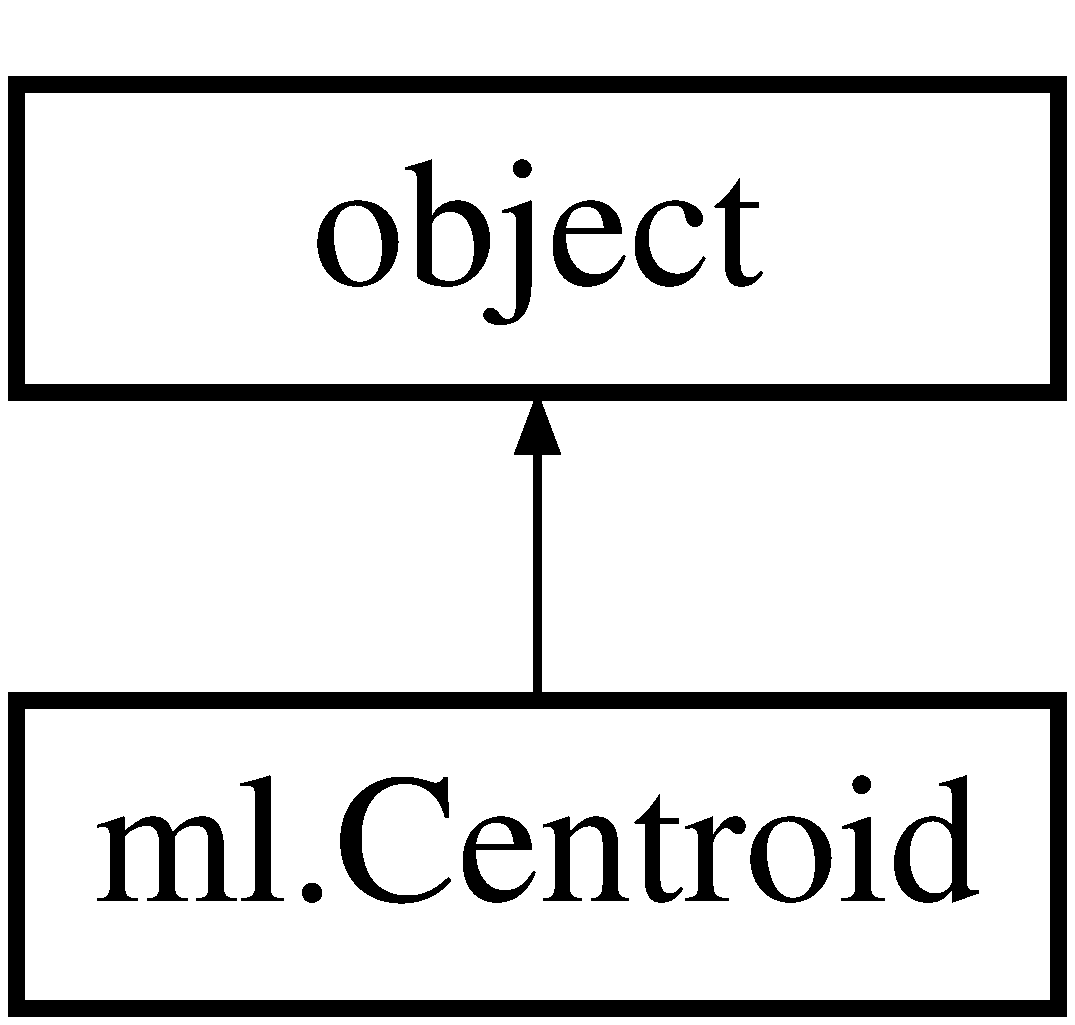
\includegraphics[height=2.000000cm]{classml_1_1Centroid}
\end{center}
\end{figure}
\subsubsection*{Public Member Functions}
\begin{DoxyCompactItemize}
\item 
def \hyperlink{classml_1_1Centroid_ad867dc3bdcf31ff91963990e903d2f1d}{\-\_\-\-\_\-init\-\_\-\-\_\-}
\item 
def \hyperlink{classml_1_1Centroid_aefdc64e2f2d22bd3609da26c0637a947}{add}
\item 
def \hyperlink{classml_1_1Centroid_a746c2a70a4573d307a3f612f9df346a5}{average}
\item 
def \hyperlink{classml_1_1Centroid_a200c3b51f7fd4bc249b6988e4d836d11}{plot}
\end{DoxyCompactItemize}
\subsubsection*{Public Attributes}
\begin{DoxyCompactItemize}
\item 
\hyperlink{classml_1_1Centroid_aff3c1bad9f79a88616bbfa01e04cca38}{instance}
\item 
\hyperlink{classml_1_1Centroid_a726bacc6a5580b80ec4f088700c16c32}{n\-Instances}
\end{DoxyCompactItemize}


\subsubsection{Constructor \& Destructor Documentation}
\hypertarget{classml_1_1Centroid_ad867dc3bdcf31ff91963990e903d2f1d}{\index{ml\-::\-Centroid@{ml\-::\-Centroid}!\-\_\-\-\_\-init\-\_\-\-\_\-@{\-\_\-\-\_\-init\-\_\-\-\_\-}}
\index{\-\_\-\-\_\-init\-\_\-\-\_\-@{\-\_\-\-\_\-init\-\_\-\-\_\-}!ml::Centroid@{ml\-::\-Centroid}}
\paragraph[{\-\_\-\-\_\-init\-\_\-\-\_\-}]{\setlength{\rightskip}{0pt plus 5cm}def ml.\-Centroid.\-\_\-\-\_\-init\-\_\-\-\_\- (
\begin{DoxyParamCaption}
\item[{}]{self, }
\item[{}]{instance, }
\item[{}]{n\-Instances = {\ttfamily 1}}
\end{DoxyParamCaption}
)}}\label{classml_1_1Centroid_ad867dc3bdcf31ff91963990e903d2f1d}


\subsubsection{Member Function Documentation}
\hypertarget{classml_1_1Centroid_aefdc64e2f2d22bd3609da26c0637a947}{\index{ml\-::\-Centroid@{ml\-::\-Centroid}!add@{add}}
\index{add@{add}!ml::Centroid@{ml\-::\-Centroid}}
\paragraph[{add}]{\setlength{\rightskip}{0pt plus 5cm}def ml.\-Centroid.\-add (
\begin{DoxyParamCaption}
\item[{}]{self, }
\item[{}]{instance2}
\end{DoxyParamCaption}
)}}\label{classml_1_1Centroid_aefdc64e2f2d22bd3609da26c0637a947}


References ml.\-Centroid.\-instance, and ml.\-Centroid.\-n\-Instances.

\hypertarget{classml_1_1Centroid_a746c2a70a4573d307a3f612f9df346a5}{\index{ml\-::\-Centroid@{ml\-::\-Centroid}!average@{average}}
\index{average@{average}!ml::Centroid@{ml\-::\-Centroid}}
\paragraph[{average}]{\setlength{\rightskip}{0pt plus 5cm}def ml.\-Centroid.\-average (
\begin{DoxyParamCaption}
\item[{}]{c}
\end{DoxyParamCaption}
)}}\label{classml_1_1Centroid_a746c2a70a4573d307a3f612f9df346a5}


References ml.\-Centroid.\-n\-Instances.

\hypertarget{classml_1_1Centroid_a200c3b51f7fd4bc249b6988e4d836d11}{\index{ml\-::\-Centroid@{ml\-::\-Centroid}!plot@{plot}}
\index{plot@{plot}!ml::Centroid@{ml\-::\-Centroid}}
\paragraph[{plot}]{\setlength{\rightskip}{0pt plus 5cm}def ml.\-Centroid.\-plot (
\begin{DoxyParamCaption}
\item[{}]{self, }
\item[{}]{options = {\ttfamily ''}}
\end{DoxyParamCaption}
)}}\label{classml_1_1Centroid_a200c3b51f7fd4bc249b6988e4d836d11}


References ml.\-Centroid.\-n\-Instances.



\subsubsection{Member Data Documentation}
\hypertarget{classml_1_1Centroid_aff3c1bad9f79a88616bbfa01e04cca38}{\index{ml\-::\-Centroid@{ml\-::\-Centroid}!instance@{instance}}
\index{instance@{instance}!ml::Centroid@{ml\-::\-Centroid}}
\paragraph[{instance}]{\setlength{\rightskip}{0pt plus 5cm}ml.\-Centroid.\-instance}}\label{classml_1_1Centroid_aff3c1bad9f79a88616bbfa01e04cca38}
\hypertarget{classml_1_1Centroid_a726bacc6a5580b80ec4f088700c16c32}{\index{ml\-::\-Centroid@{ml\-::\-Centroid}!n\-Instances@{n\-Instances}}
\index{n\-Instances@{n\-Instances}!ml::Centroid@{ml\-::\-Centroid}}
\paragraph[{n\-Instances}]{\setlength{\rightskip}{0pt plus 5cm}ml.\-Centroid.\-n\-Instances}}\label{classml_1_1Centroid_a726bacc6a5580b80ec4f088700c16c32}


The documentation for this class was generated from the following file\-:\begin{DoxyCompactItemize}
\item 
python/\hyperlink{ml_8py}{ml.\-py}\end{DoxyCompactItemize}

\hypertarget{classColors}{\subsection{Colors Class Reference}
\label{classColors}\index{Colors@{Colors}}
}


Pre-\/defined colors.  




{\ttfamily \#include $<$cvutils.\-hpp$>$}

\subsubsection*{Static Public Member Functions}
\begin{DoxyCompactItemize}
\item 
static cv\-::\-Scalar \hyperlink{classColors_aec5500a7bacaf540790954b251cb859e}{black} (void)
\item 
static cv\-::\-Scalar \hyperlink{classColors_ac9355f317c0aca8cb6c1329c996b52ff}{red} (void)
\item 
static cv\-::\-Scalar \hyperlink{classColors_a2e5a3b8a640c9a9d986a6f9edc60e14e}{green} (void)
\item 
static cv\-::\-Scalar \hyperlink{classColors_a35176ed2a7964fd7ccac8e4bb61c1a59}{blue} (void)
\item 
static cv\-::\-Scalar \hyperlink{classColors_ad923407109a41ab191b3c70756868245}{white} (void)
\item 
static cv\-::\-Scalar \hyperlink{classColors_acac58cf111796f98f7f851ec8dac3c56}{magenta} (void)
\item 
static cv\-::\-Scalar \hyperlink{classColors_aaeddb3283139623d18df416ec5cb7d4f}{cyan} (void)
\item 
static cv\-::\-Scalar \hyperlink{classColors_a803953241028654107321e46d9ae78d5}{yellow} (void)
\item 
static cv\-::\-Scalar \hyperlink{classColors_a44c783202f4a41371ff85e80df478109}{color3} (const int \&num)
\item 
static cv\-::\-Scalar \hyperlink{classColors_aac2bcf82724d40923e52543606b22628}{color8} (const int \&num)
\end{DoxyCompactItemize}
\subsubsection*{Static Public Attributes}
\begin{DoxyCompactItemize}
\item 
static const int \hyperlink{classColors_a5175069a56ae9ccfcb35b1688e1926ad}{n\-Colors} = 8
\item 
static const cv\-::\-Scalar \hyperlink{classColors_aa4ba92c3d309c4f93bf10cc0fe2e2d3b}{color} \mbox{[}$\,$\mbox{]}
\end{DoxyCompactItemize}


\subsubsection{Detailed Description}
Pre-\/defined colors. 

Allocates a new Ipl\-Image. Goes to the target frame number, by querying frame, supposing the video input is currently at current frame number. Returns the frame number that was reached. 

\subsubsection{Member Function Documentation}
\hypertarget{classColors_aec5500a7bacaf540790954b251cb859e}{\index{Colors@{Colors}!black@{black}}
\index{black@{black}!Colors@{Colors}}
\paragraph[{black}]{\setlength{\rightskip}{0pt plus 5cm}Scalar Colors\-::black (
\begin{DoxyParamCaption}
\item[{void}]{}
\end{DoxyParamCaption}
)\hspace{0.3cm}{\ttfamily [static]}}}\label{classColors_aec5500a7bacaf540790954b251cb859e}
\hypertarget{classColors_a35176ed2a7964fd7ccac8e4bb61c1a59}{\index{Colors@{Colors}!blue@{blue}}
\index{blue@{blue}!Colors@{Colors}}
\paragraph[{blue}]{\setlength{\rightskip}{0pt plus 5cm}Scalar Colors\-::blue (
\begin{DoxyParamCaption}
\item[{void}]{}
\end{DoxyParamCaption}
)\hspace{0.3cm}{\ttfamily [static]}}}\label{classColors_a35176ed2a7964fd7ccac8e4bb61c1a59}
\hypertarget{classColors_a44c783202f4a41371ff85e80df478109}{\index{Colors@{Colors}!color3@{color3}}
\index{color3@{color3}!Colors@{Colors}}
\paragraph[{color3}]{\setlength{\rightskip}{0pt plus 5cm}Scalar Colors\-::color3 (
\begin{DoxyParamCaption}
\item[{const int \&}]{num}
\end{DoxyParamCaption}
)\hspace{0.3cm}{\ttfamily [static]}}}\label{classColors_a44c783202f4a41371ff85e80df478109}
Maps integers to primary colors. 

References color.

\hypertarget{classColors_aac2bcf82724d40923e52543606b22628}{\index{Colors@{Colors}!color8@{color8}}
\index{color8@{color8}!Colors@{Colors}}
\paragraph[{color8}]{\setlength{\rightskip}{0pt plus 5cm}Scalar Colors\-::color8 (
\begin{DoxyParamCaption}
\item[{const int \&}]{num}
\end{DoxyParamCaption}
)\hspace{0.3cm}{\ttfamily [static]}}}\label{classColors_aac2bcf82724d40923e52543606b22628}


References color, and n\-Colors.

\hypertarget{classColors_aaeddb3283139623d18df416ec5cb7d4f}{\index{Colors@{Colors}!cyan@{cyan}}
\index{cyan@{cyan}!Colors@{Colors}}
\paragraph[{cyan}]{\setlength{\rightskip}{0pt plus 5cm}Scalar Colors\-::cyan (
\begin{DoxyParamCaption}
\item[{void}]{}
\end{DoxyParamCaption}
)\hspace{0.3cm}{\ttfamily [static]}}}\label{classColors_aaeddb3283139623d18df416ec5cb7d4f}
\hypertarget{classColors_a2e5a3b8a640c9a9d986a6f9edc60e14e}{\index{Colors@{Colors}!green@{green}}
\index{green@{green}!Colors@{Colors}}
\paragraph[{green}]{\setlength{\rightskip}{0pt plus 5cm}Scalar Colors\-::green (
\begin{DoxyParamCaption}
\item[{void}]{}
\end{DoxyParamCaption}
)\hspace{0.3cm}{\ttfamily [static]}}}\label{classColors_a2e5a3b8a640c9a9d986a6f9edc60e14e}
\hypertarget{classColors_acac58cf111796f98f7f851ec8dac3c56}{\index{Colors@{Colors}!magenta@{magenta}}
\index{magenta@{magenta}!Colors@{Colors}}
\paragraph[{magenta}]{\setlength{\rightskip}{0pt plus 5cm}Scalar Colors\-::magenta (
\begin{DoxyParamCaption}
\item[{void}]{}
\end{DoxyParamCaption}
)\hspace{0.3cm}{\ttfamily [static]}}}\label{classColors_acac58cf111796f98f7f851ec8dac3c56}
\hypertarget{classColors_ac9355f317c0aca8cb6c1329c996b52ff}{\index{Colors@{Colors}!red@{red}}
\index{red@{red}!Colors@{Colors}}
\paragraph[{red}]{\setlength{\rightskip}{0pt plus 5cm}Scalar Colors\-::red (
\begin{DoxyParamCaption}
\item[{void}]{}
\end{DoxyParamCaption}
)\hspace{0.3cm}{\ttfamily [static]}}}\label{classColors_ac9355f317c0aca8cb6c1329c996b52ff}
\hypertarget{classColors_ad923407109a41ab191b3c70756868245}{\index{Colors@{Colors}!white@{white}}
\index{white@{white}!Colors@{Colors}}
\paragraph[{white}]{\setlength{\rightskip}{0pt plus 5cm}Scalar Colors\-::white (
\begin{DoxyParamCaption}
\item[{void}]{}
\end{DoxyParamCaption}
)\hspace{0.3cm}{\ttfamily [static]}}}\label{classColors_ad923407109a41ab191b3c70756868245}
\hypertarget{classColors_a803953241028654107321e46d9ae78d5}{\index{Colors@{Colors}!yellow@{yellow}}
\index{yellow@{yellow}!Colors@{Colors}}
\paragraph[{yellow}]{\setlength{\rightskip}{0pt plus 5cm}Scalar Colors\-::yellow (
\begin{DoxyParamCaption}
\item[{void}]{}
\end{DoxyParamCaption}
)\hspace{0.3cm}{\ttfamily [static]}}}\label{classColors_a803953241028654107321e46d9ae78d5}


\subsubsection{Member Data Documentation}
\hypertarget{classColors_aa4ba92c3d309c4f93bf10cc0fe2e2d3b}{\index{Colors@{Colors}!color@{color}}
\index{color@{color}!Colors@{Colors}}
\paragraph[{color}]{\setlength{\rightskip}{0pt plus 5cm}const Scalar Colors\-::color\hspace{0.3cm}{\ttfamily [static]}}}\label{classColors_aa4ba92c3d309c4f93bf10cc0fe2e2d3b}
{\bfseries Initial value\-:}
\begin{DoxyCode}
= \{\hyperlink{classColors_ac9355f317c0aca8cb6c1329c996b52ff}{Colors::red}(),
                                \hyperlink{classColors_a2e5a3b8a640c9a9d986a6f9edc60e14e}{Colors::green}(),
                                \hyperlink{classColors_a35176ed2a7964fd7ccac8e4bb61c1a59}{Colors::blue}(),
                                \hyperlink{classColors_aaeddb3283139623d18df416ec5cb7d4f}{Colors::cyan}(), 
                                \hyperlink{classColors_acac58cf111796f98f7f851ec8dac3c56}{Colors::magenta}(), 
                                \hyperlink{classColors_a803953241028654107321e46d9ae78d5}{Colors::yellow}(), 
                                \hyperlink{classColors_ad923407109a41ab191b3c70756868245}{Colors::white}(), 
                                \hyperlink{classColors_aec5500a7bacaf540790954b251cb859e}{Colors::black}()\}
\end{DoxyCode}
\hypertarget{classColors_a5175069a56ae9ccfcb35b1688e1926ad}{\index{Colors@{Colors}!n\-Colors@{n\-Colors}}
\index{n\-Colors@{n\-Colors}!Colors@{Colors}}
\paragraph[{n\-Colors}]{\setlength{\rightskip}{0pt plus 5cm}const int Colors\-::n\-Colors = 8\hspace{0.3cm}{\ttfamily [static]}}}\label{classColors_a5175069a56ae9ccfcb35b1688e1926ad}


The documentation for this class was generated from the following files\-:\begin{DoxyCompactItemize}
\item 
include/\hyperlink{cvutils_8hpp}{cvutils.\-hpp}\item 
c/\hyperlink{cvutils_8cpp}{cvutils.\-cpp}\end{DoxyCompactItemize}

\hypertarget{classCatch_1_1CompositeGenerator}{\subsection{Catch\-:\-:Composite\-Generator$<$ T $>$ Class Template Reference}
\label{classCatch_1_1CompositeGenerator}\index{Catch\-::\-Composite\-Generator$<$ T $>$@{Catch\-::\-Composite\-Generator$<$ T $>$}}
}


{\ttfamily \#include $<$catch.\-hpp$>$}

\subsubsection*{Public Member Functions}
\begin{DoxyCompactItemize}
\item 
\hyperlink{classCatch_1_1CompositeGenerator_a923398b140371d1783858766864a1af5}{Composite\-Generator} ()
\item 
\hyperlink{classCatch_1_1CompositeGenerator_a21a7070a00e4a6fe021294c356692692}{Composite\-Generator} (\hyperlink{classCatch_1_1CompositeGenerator}{Composite\-Generator} \&other)
\item 
\hyperlink{classCatch_1_1CompositeGenerator}{Composite\-Generator} \& \hyperlink{classCatch_1_1CompositeGenerator_ac3c57cf4ca5472f440bf71e2936bcd4a}{set\-File\-Info} (const char $\ast$file\-Info)
\item 
\hyperlink{classCatch_1_1CompositeGenerator_a5766205abd7004c508c20ddbb5e5555e}{$\sim$\-Composite\-Generator} ()
\item 
\hyperlink{classCatch_1_1CompositeGenerator_aa3f627d84fb256df0404d19d7fd4b784}{operator T} () const 
\item 
void \hyperlink{classCatch_1_1CompositeGenerator_af3774d42ad2d3453d089ca599efe0517}{add} (const \hyperlink{structCatch_1_1IGenerator}{I\-Generator}$<$ T $>$ $\ast$generator)
\item 
\hyperlink{classCatch_1_1CompositeGenerator}{Composite\-Generator} \& \hyperlink{classCatch_1_1CompositeGenerator_a2e03f42df85cdd238aabd77a80b075d5}{then} (\hyperlink{classCatch_1_1CompositeGenerator}{Composite\-Generator} \&other)
\item 
\hyperlink{classCatch_1_1CompositeGenerator}{Composite\-Generator} \& \hyperlink{classCatch_1_1CompositeGenerator_aefdc11bcfccdf07d2db5f0da3ed8758c}{then} (T value)
\end{DoxyCompactItemize}


\subsubsection{Constructor \& Destructor Documentation}
\hypertarget{classCatch_1_1CompositeGenerator_a923398b140371d1783858766864a1af5}{\index{Catch\-::\-Composite\-Generator@{Catch\-::\-Composite\-Generator}!Composite\-Generator@{Composite\-Generator}}
\index{Composite\-Generator@{Composite\-Generator}!Catch::CompositeGenerator@{Catch\-::\-Composite\-Generator}}
\paragraph[{Composite\-Generator}]{\setlength{\rightskip}{0pt plus 5cm}template$<$typename T$>$ {\bf Catch\-::\-Composite\-Generator}$<$ T $>$\-::{\bf Composite\-Generator} (
\begin{DoxyParamCaption}
{}
\end{DoxyParamCaption}
)\hspace{0.3cm}{\ttfamily [inline]}}}\label{classCatch_1_1CompositeGenerator_a923398b140371d1783858766864a1af5}
\hypertarget{classCatch_1_1CompositeGenerator_a21a7070a00e4a6fe021294c356692692}{\index{Catch\-::\-Composite\-Generator@{Catch\-::\-Composite\-Generator}!Composite\-Generator@{Composite\-Generator}}
\index{Composite\-Generator@{Composite\-Generator}!Catch::CompositeGenerator@{Catch\-::\-Composite\-Generator}}
\paragraph[{Composite\-Generator}]{\setlength{\rightskip}{0pt plus 5cm}template$<$typename T$>$ {\bf Catch\-::\-Composite\-Generator}$<$ T $>$\-::{\bf Composite\-Generator} (
\begin{DoxyParamCaption}
\item[{{\bf Composite\-Generator}$<$ T $>$ \&}]{other}
\end{DoxyParamCaption}
)\hspace{0.3cm}{\ttfamily [inline]}}}\label{classCatch_1_1CompositeGenerator_a21a7070a00e4a6fe021294c356692692}
\hypertarget{classCatch_1_1CompositeGenerator_a5766205abd7004c508c20ddbb5e5555e}{\index{Catch\-::\-Composite\-Generator@{Catch\-::\-Composite\-Generator}!$\sim$\-Composite\-Generator@{$\sim$\-Composite\-Generator}}
\index{$\sim$\-Composite\-Generator@{$\sim$\-Composite\-Generator}!Catch::CompositeGenerator@{Catch\-::\-Composite\-Generator}}
\paragraph[{$\sim$\-Composite\-Generator}]{\setlength{\rightskip}{0pt plus 5cm}template$<$typename T$>$ {\bf Catch\-::\-Composite\-Generator}$<$ T $>$\-::$\sim${\bf Composite\-Generator} (
\begin{DoxyParamCaption}
{}
\end{DoxyParamCaption}
)\hspace{0.3cm}{\ttfamily [inline]}}}\label{classCatch_1_1CompositeGenerator_a5766205abd7004c508c20ddbb5e5555e}


References Catch\-::delete\-All().



\subsubsection{Member Function Documentation}
\hypertarget{classCatch_1_1CompositeGenerator_af3774d42ad2d3453d089ca599efe0517}{\index{Catch\-::\-Composite\-Generator@{Catch\-::\-Composite\-Generator}!add@{add}}
\index{add@{add}!Catch::CompositeGenerator@{Catch\-::\-Composite\-Generator}}
\paragraph[{add}]{\setlength{\rightskip}{0pt plus 5cm}template$<$typename T$>$ void {\bf Catch\-::\-Composite\-Generator}$<$ T $>$\-::add (
\begin{DoxyParamCaption}
\item[{const {\bf I\-Generator}$<$ T $>$ $\ast$}]{generator}
\end{DoxyParamCaption}
)\hspace{0.3cm}{\ttfamily [inline]}}}\label{classCatch_1_1CompositeGenerator_af3774d42ad2d3453d089ca599efe0517}


References Catch\-::\-I\-Generator$<$ T $>$\-::size().

\hypertarget{classCatch_1_1CompositeGenerator_aa3f627d84fb256df0404d19d7fd4b784}{\index{Catch\-::\-Composite\-Generator@{Catch\-::\-Composite\-Generator}!operator T@{operator T}}
\index{operator T@{operator T}!Catch::CompositeGenerator@{Catch\-::\-Composite\-Generator}}
\paragraph[{operator T}]{\setlength{\rightskip}{0pt plus 5cm}template$<$typename T$>$ {\bf Catch\-::\-Composite\-Generator}$<$ T $>$\-::operator T (
\begin{DoxyParamCaption}
{}
\end{DoxyParamCaption}
) const\hspace{0.3cm}{\ttfamily [inline]}}}\label{classCatch_1_1CompositeGenerator_aa3f627d84fb256df0404d19d7fd4b784}


References C\-A\-T\-C\-H\-\_\-\-I\-N\-T\-E\-R\-N\-A\-L\-\_\-\-E\-R\-R\-O\-R, Catch\-::get\-Current\-Context(), Catch\-::\-I\-Context\-::get\-Generator\-Index(), Catch\-::\-I\-Generator$<$ T $>$\-::get\-Value(), and Catch\-::\-I\-Generator$<$ T $>$\-::size().

\hypertarget{classCatch_1_1CompositeGenerator_ac3c57cf4ca5472f440bf71e2936bcd4a}{\index{Catch\-::\-Composite\-Generator@{Catch\-::\-Composite\-Generator}!set\-File\-Info@{set\-File\-Info}}
\index{set\-File\-Info@{set\-File\-Info}!Catch::CompositeGenerator@{Catch\-::\-Composite\-Generator}}
\paragraph[{set\-File\-Info}]{\setlength{\rightskip}{0pt plus 5cm}template$<$typename T$>$ {\bf Composite\-Generator}\& {\bf Catch\-::\-Composite\-Generator}$<$ T $>$\-::set\-File\-Info (
\begin{DoxyParamCaption}
\item[{const char $\ast$}]{file\-Info}
\end{DoxyParamCaption}
)\hspace{0.3cm}{\ttfamily [inline]}}}\label{classCatch_1_1CompositeGenerator_ac3c57cf4ca5472f440bf71e2936bcd4a}
\hypertarget{classCatch_1_1CompositeGenerator_a2e03f42df85cdd238aabd77a80b075d5}{\index{Catch\-::\-Composite\-Generator@{Catch\-::\-Composite\-Generator}!then@{then}}
\index{then@{then}!Catch::CompositeGenerator@{Catch\-::\-Composite\-Generator}}
\paragraph[{then}]{\setlength{\rightskip}{0pt plus 5cm}template$<$typename T$>$ {\bf Composite\-Generator}\& {\bf Catch\-::\-Composite\-Generator}$<$ T $>$\-::then (
\begin{DoxyParamCaption}
\item[{{\bf Composite\-Generator}$<$ T $>$ \&}]{other}
\end{DoxyParamCaption}
)\hspace{0.3cm}{\ttfamily [inline]}}}\label{classCatch_1_1CompositeGenerator_a2e03f42df85cdd238aabd77a80b075d5}
\hypertarget{classCatch_1_1CompositeGenerator_aefdc11bcfccdf07d2db5f0da3ed8758c}{\index{Catch\-::\-Composite\-Generator@{Catch\-::\-Composite\-Generator}!then@{then}}
\index{then@{then}!Catch::CompositeGenerator@{Catch\-::\-Composite\-Generator}}
\paragraph[{then}]{\setlength{\rightskip}{0pt plus 5cm}template$<$typename T$>$ {\bf Composite\-Generator}\& {\bf Catch\-::\-Composite\-Generator}$<$ T $>$\-::then (
\begin{DoxyParamCaption}
\item[{T}]{value}
\end{DoxyParamCaption}
)\hspace{0.3cm}{\ttfamily [inline]}}}\label{classCatch_1_1CompositeGenerator_aefdc11bcfccdf07d2db5f0da3ed8758c}


References Catch\-::\-Values\-Generator$<$ T $>$\-::add(), and Catch\-::\-Composite\-Generator$<$ T $>$\-::add().



The documentation for this class was generated from the following file\-:\begin{DoxyCompactItemize}
\item 
include/\hyperlink{catch_8hpp}{catch.\-hpp}\end{DoxyCompactItemize}

\hypertarget{classprediction_1_1ConstantPredictionParameters}{\subsection{prediction.\-Constant\-Prediction\-Parameters Class Reference}
\label{classprediction_1_1ConstantPredictionParameters}\index{prediction.\-Constant\-Prediction\-Parameters@{prediction.\-Constant\-Prediction\-Parameters}}
}
Inheritance diagram for prediction.\-Constant\-Prediction\-Parameters\-:\begin{figure}[H]
\begin{center}
\leavevmode
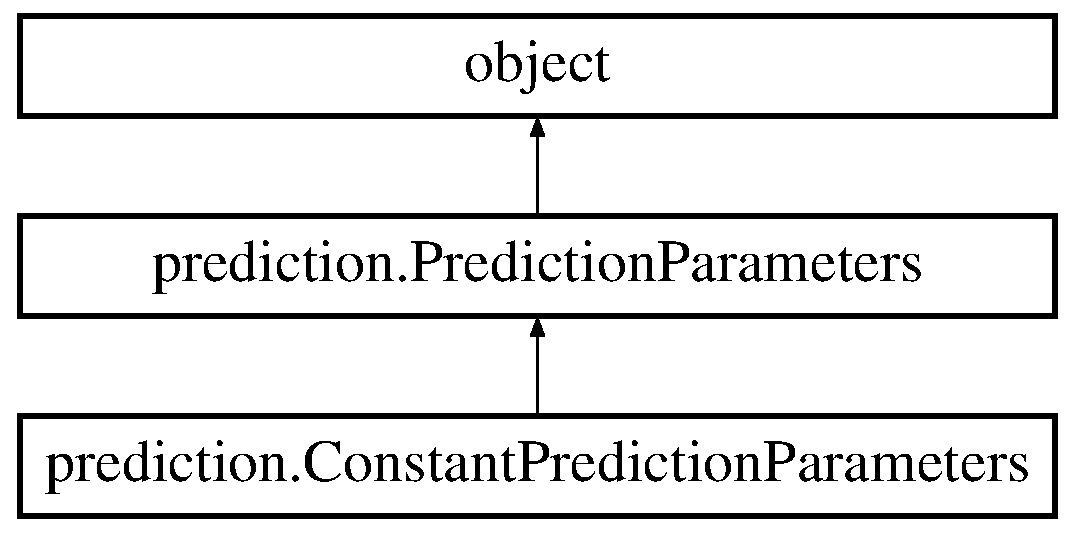
\includegraphics[height=3.000000cm]{classprediction_1_1ConstantPredictionParameters}
\end{center}
\end{figure}
\subsubsection*{Public Member Functions}
\begin{DoxyCompactItemize}
\item 
def \hyperlink{classprediction_1_1ConstantPredictionParameters_a37a0f2c83ec75e0180752568d82395bc}{\-\_\-\-\_\-init\-\_\-\-\_\-}
\item 
def \hyperlink{classprediction_1_1ConstantPredictionParameters_aebdbd1bf7ed910f93f2127bdb0e17998}{generate\-Predicted\-Trajectories}
\end{DoxyCompactItemize}
\subsubsection*{Additional Inherited Members}


\subsubsection{Constructor \& Destructor Documentation}
\hypertarget{classprediction_1_1ConstantPredictionParameters_a37a0f2c83ec75e0180752568d82395bc}{\index{prediction\-::\-Constant\-Prediction\-Parameters@{prediction\-::\-Constant\-Prediction\-Parameters}!\-\_\-\-\_\-init\-\_\-\-\_\-@{\-\_\-\-\_\-init\-\_\-\-\_\-}}
\index{\-\_\-\-\_\-init\-\_\-\-\_\-@{\-\_\-\-\_\-init\-\_\-\-\_\-}!prediction::ConstantPredictionParameters@{prediction\-::\-Constant\-Prediction\-Parameters}}
\paragraph[{\-\_\-\-\_\-init\-\_\-\-\_\-}]{\setlength{\rightskip}{0pt plus 5cm}def prediction.\-Constant\-Prediction\-Parameters.\-\_\-\-\_\-init\-\_\-\-\_\- (
\begin{DoxyParamCaption}
\item[{}]{self, }
\item[{}]{max\-Speed}
\end{DoxyParamCaption}
)}}\label{classprediction_1_1ConstantPredictionParameters_a37a0f2c83ec75e0180752568d82395bc}


\subsubsection{Member Function Documentation}
\hypertarget{classprediction_1_1ConstantPredictionParameters_aebdbd1bf7ed910f93f2127bdb0e17998}{\index{prediction\-::\-Constant\-Prediction\-Parameters@{prediction\-::\-Constant\-Prediction\-Parameters}!generate\-Predicted\-Trajectories@{generate\-Predicted\-Trajectories}}
\index{generate\-Predicted\-Trajectories@{generate\-Predicted\-Trajectories}!prediction::ConstantPredictionParameters@{prediction\-::\-Constant\-Prediction\-Parameters}}
\paragraph[{generate\-Predicted\-Trajectories}]{\setlength{\rightskip}{0pt plus 5cm}def prediction.\-Constant\-Prediction\-Parameters.\-generate\-Predicted\-Trajectories (
\begin{DoxyParamCaption}
\item[{}]{self, }
\item[{}]{obj, }
\item[{}]{instant}
\end{DoxyParamCaption}
)}}\label{classprediction_1_1ConstantPredictionParameters_aebdbd1bf7ed910f93f2127bdb0e17998}


References prediction.\-Predicted\-Trajectory\-Constant.\-max\-Speed, prediction.\-Predicted\-Trajectory\-Random\-Control.\-max\-Speed, and prediction.\-Prediction\-Parameters.\-max\-Speed.



The documentation for this class was generated from the following file\-:\begin{DoxyCompactItemize}
\item 
python/\hyperlink{prediction_8py}{prediction.\-py}\end{DoxyCompactItemize}

\hypertarget{structCatch_1_1Matchers_1_1Impl_1_1StdString_1_1Contains}{\subsection{Catch\-:\-:Matchers\-:\-:Impl\-:\-:Std\-String\-:\-:Contains Struct Reference}
\label{structCatch_1_1Matchers_1_1Impl_1_1StdString_1_1Contains}\index{Catch\-::\-Matchers\-::\-Impl\-::\-Std\-String\-::\-Contains@{Catch\-::\-Matchers\-::\-Impl\-::\-Std\-String\-::\-Contains}}
}


{\ttfamily \#include $<$catch.\-hpp$>$}

\subsubsection*{Public Member Functions}
\begin{DoxyCompactItemize}
\item 
\hyperlink{structCatch_1_1Matchers_1_1Impl_1_1StdString_1_1Contains_a329b03ab3a18970ed0612f4387a554a4}{Contains} (const std\-::string \&substr)
\item 
bool \hyperlink{structCatch_1_1Matchers_1_1Impl_1_1StdString_1_1Contains_a00b2607249ca28c81a1aced2a5c77b8f}{operator()} (const std\-::string \&str) const 
\end{DoxyCompactItemize}
\subsubsection*{Public Attributes}
\begin{DoxyCompactItemize}
\item 
std\-::string \hyperlink{structCatch_1_1Matchers_1_1Impl_1_1StdString_1_1Contains_a0bad82dd7cbdd0ec06b6d562181db03e}{m\-\_\-substr}
\end{DoxyCompactItemize}
\subsubsection*{Friends}
\begin{DoxyCompactItemize}
\item 
std\-::ostream \& \hyperlink{structCatch_1_1Matchers_1_1Impl_1_1StdString_1_1Contains_a8df8dcad0e24173b72cb72dcd0d1d1e0}{operator$<$$<$} (std\-::ostream \&os, const \hyperlink{structCatch_1_1Matchers_1_1Impl_1_1StdString_1_1Contains}{Contains} \&matcher)
\end{DoxyCompactItemize}


\subsubsection{Constructor \& Destructor Documentation}
\hypertarget{structCatch_1_1Matchers_1_1Impl_1_1StdString_1_1Contains_a329b03ab3a18970ed0612f4387a554a4}{\index{Catch\-::\-Matchers\-::\-Impl\-::\-Std\-String\-::\-Contains@{Catch\-::\-Matchers\-::\-Impl\-::\-Std\-String\-::\-Contains}!Contains@{Contains}}
\index{Contains@{Contains}!Catch::Matchers::Impl::StdString::Contains@{Catch\-::\-Matchers\-::\-Impl\-::\-Std\-String\-::\-Contains}}
\paragraph[{Contains}]{\setlength{\rightskip}{0pt plus 5cm}Catch\-::\-Matchers\-::\-Impl\-::\-Std\-String\-::\-Contains\-::\-Contains (
\begin{DoxyParamCaption}
\item[{const std\-::string \&}]{substr}
\end{DoxyParamCaption}
)\hspace{0.3cm}{\ttfamily [inline]}}}\label{structCatch_1_1Matchers_1_1Impl_1_1StdString_1_1Contains_a329b03ab3a18970ed0612f4387a554a4}


\subsubsection{Member Function Documentation}
\hypertarget{structCatch_1_1Matchers_1_1Impl_1_1StdString_1_1Contains_a00b2607249ca28c81a1aced2a5c77b8f}{\index{Catch\-::\-Matchers\-::\-Impl\-::\-Std\-String\-::\-Contains@{Catch\-::\-Matchers\-::\-Impl\-::\-Std\-String\-::\-Contains}!operator()@{operator()}}
\index{operator()@{operator()}!Catch::Matchers::Impl::StdString::Contains@{Catch\-::\-Matchers\-::\-Impl\-::\-Std\-String\-::\-Contains}}
\paragraph[{operator()}]{\setlength{\rightskip}{0pt plus 5cm}bool Catch\-::\-Matchers\-::\-Impl\-::\-Std\-String\-::\-Contains\-::operator() (
\begin{DoxyParamCaption}
\item[{const std\-::string \&}]{str}
\end{DoxyParamCaption}
) const\hspace{0.3cm}{\ttfamily [inline]}}}\label{structCatch_1_1Matchers_1_1Impl_1_1StdString_1_1Contains_a00b2607249ca28c81a1aced2a5c77b8f}


References m\-\_\-substr.



\subsubsection{Friends And Related Function Documentation}
\hypertarget{structCatch_1_1Matchers_1_1Impl_1_1StdString_1_1Contains_a8df8dcad0e24173b72cb72dcd0d1d1e0}{\index{Catch\-::\-Matchers\-::\-Impl\-::\-Std\-String\-::\-Contains@{Catch\-::\-Matchers\-::\-Impl\-::\-Std\-String\-::\-Contains}!operator$<$$<$@{operator$<$$<$}}
\index{operator$<$$<$@{operator$<$$<$}!Catch::Matchers::Impl::StdString::Contains@{Catch\-::\-Matchers\-::\-Impl\-::\-Std\-String\-::\-Contains}}
\paragraph[{operator$<$$<$}]{\setlength{\rightskip}{0pt plus 5cm}std\-::ostream\& operator$<$$<$ (
\begin{DoxyParamCaption}
\item[{std\-::ostream \&}]{os, }
\item[{const {\bf Contains} \&}]{matcher}
\end{DoxyParamCaption}
)\hspace{0.3cm}{\ttfamily [friend]}}}\label{structCatch_1_1Matchers_1_1Impl_1_1StdString_1_1Contains_a8df8dcad0e24173b72cb72dcd0d1d1e0}


\subsubsection{Member Data Documentation}
\hypertarget{structCatch_1_1Matchers_1_1Impl_1_1StdString_1_1Contains_a0bad82dd7cbdd0ec06b6d562181db03e}{\index{Catch\-::\-Matchers\-::\-Impl\-::\-Std\-String\-::\-Contains@{Catch\-::\-Matchers\-::\-Impl\-::\-Std\-String\-::\-Contains}!m\-\_\-substr@{m\-\_\-substr}}
\index{m\-\_\-substr@{m\-\_\-substr}!Catch::Matchers::Impl::StdString::Contains@{Catch\-::\-Matchers\-::\-Impl\-::\-Std\-String\-::\-Contains}}
\paragraph[{m\-\_\-substr}]{\setlength{\rightskip}{0pt plus 5cm}std\-::string Catch\-::\-Matchers\-::\-Impl\-::\-Std\-String\-::\-Contains\-::m\-\_\-substr}}\label{structCatch_1_1Matchers_1_1Impl_1_1StdString_1_1Contains_a0bad82dd7cbdd0ec06b6d562181db03e}


The documentation for this struct was generated from the following file\-:\begin{DoxyCompactItemize}
\item 
include/\hyperlink{catch_8hpp}{catch.\-hpp}\end{DoxyCompactItemize}

\hypertarget{classCatch_1_1Context}{\subsection{Catch\-:\-:Context Class Reference}
\label{classCatch_1_1Context}\index{Catch\-::\-Context@{Catch\-::\-Context}}
}


{\ttfamily \#include $<$catch.\-hpp$>$}

Inheritance diagram for Catch\-:\-:Context\-:\begin{figure}[H]
\begin{center}
\leavevmode
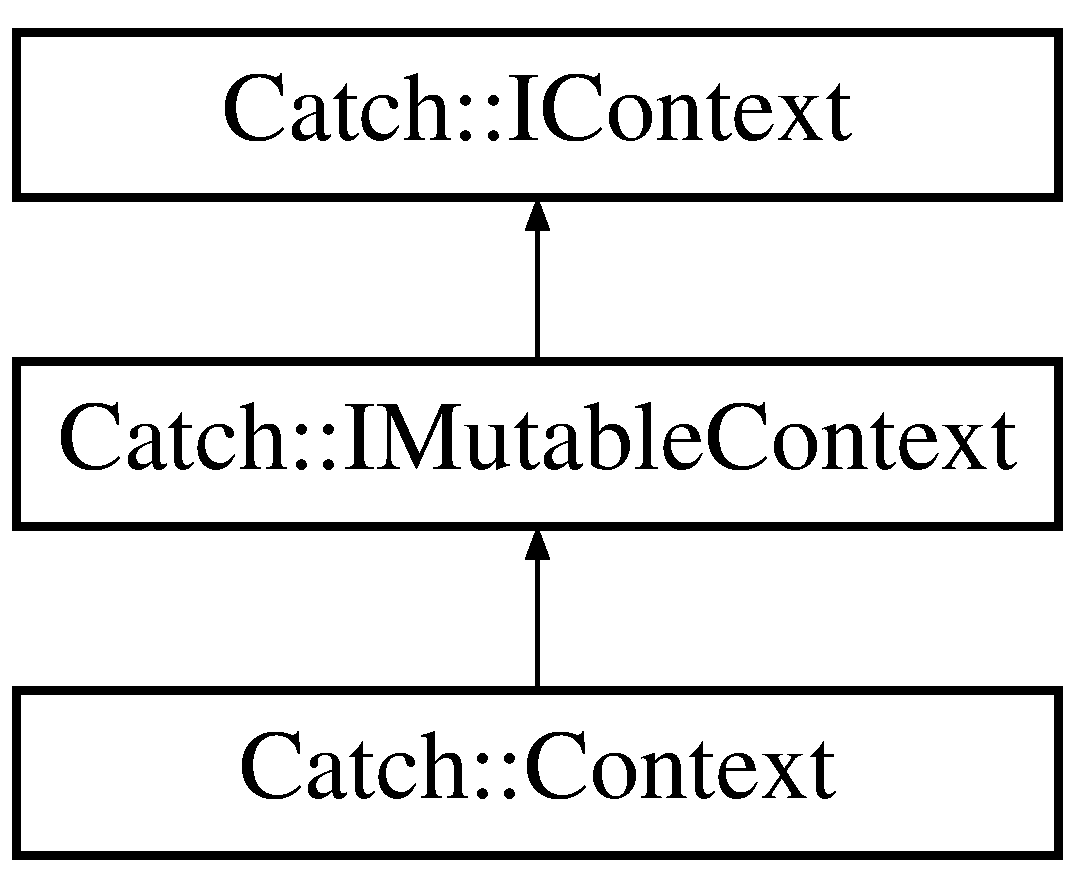
\includegraphics[height=3.000000cm]{classCatch_1_1Context}
\end{center}
\end{figure}
\subsubsection*{Public Member Functions}
\begin{DoxyCompactItemize}
\item 
virtual \hyperlink{structCatch_1_1IResultCapture}{I\-Result\-Capture} \& \hyperlink{classCatch_1_1Context_ae28e8862c120382a5747ffc36611271b}{get\-Result\-Capture} ()
\item 
virtual \hyperlink{structCatch_1_1IRunner}{I\-Runner} \& \hyperlink{classCatch_1_1Context_aa28c1fa65249a6b344d8574c3f345525}{get\-Runner} ()
\item 
virtual \hyperlink{structCatch_1_1IReporterRegistry}{I\-Reporter\-Registry} \& \hyperlink{classCatch_1_1Context_aad092bba66a990c412eb5137e8a8d1fd}{get\-Reporter\-Registry} ()
\item 
virtual \hyperlink{structCatch_1_1ITestCaseRegistry}{I\-Test\-Case\-Registry} \& \hyperlink{classCatch_1_1Context_a4355723154f927cacb75f5894f599627}{get\-Test\-Case\-Registry} ()
\item 
virtual \\*
\hyperlink{structCatch_1_1IExceptionTranslatorRegistry}{I\-Exception\-Translator\-Registry} \& \hyperlink{classCatch_1_1Context_a8e3ce31c44d5b3c706a878dcdd77d7e9}{get\-Exception\-Translator\-Registry} ()
\item 
virtual size\-\_\-t \hyperlink{classCatch_1_1Context_a06474443026c33532fdfb2ea1848eb31}{get\-Generator\-Index} (const std\-::string \&file\-Info, size\-\_\-t total\-Size)
\item 
virtual bool \hyperlink{classCatch_1_1Context_aa4c8d900c7168191636bf54ae5c1d501}{advance\-Generators\-For\-Current\-Test} ()
\item 
virtual const \hyperlink{structCatch_1_1IConfig}{I\-Config} $\ast$ \hyperlink{classCatch_1_1Context_a352ac7605c53582bf278105396ce8f74}{get\-Config} () const 
\item 
virtual void \hyperlink{classCatch_1_1Context_acd5a98f515e43085a2d32e6c48d582b0}{set\-Result\-Capture} (\hyperlink{structCatch_1_1IResultCapture}{I\-Result\-Capture} $\ast$result\-Capture)
\item 
virtual void \hyperlink{classCatch_1_1Context_a9be76af925623d87d5692a08bf58abca}{set\-Runner} (\hyperlink{structCatch_1_1IRunner}{I\-Runner} $\ast$runner)
\item 
virtual void \hyperlink{classCatch_1_1Context_a95379b3aeaca34fb2c9a7a4424cab98c}{set\-Config} (const \hyperlink{structCatch_1_1IConfig}{I\-Config} $\ast$config)
\end{DoxyCompactItemize}
\subsubsection*{Static Public Member Functions}
\begin{DoxyCompactItemize}
\item 
static std\-::streambuf $\ast$ \hyperlink{classCatch_1_1Context_aee97866c2a6bc4d123407a6ffd637501}{create\-Stream\-Buf} (const std\-::string \&stream\-Name)
\item 
static void \hyperlink{classCatch_1_1Context_a7426fde90f2b154e42e6943db988f9ce}{clean\-Up} ()
\end{DoxyCompactItemize}
\subsubsection*{Friends}
\begin{DoxyCompactItemize}
\item 
\hyperlink{structCatch_1_1IMutableContext}{I\-Mutable\-Context} \& \hyperlink{classCatch_1_1Context_aea4b25692aaf4397cdf630716976f6b8}{get\-Current\-Mutable\-Context} ()
\end{DoxyCompactItemize}


\subsubsection{Member Function Documentation}
\hypertarget{classCatch_1_1Context_aa4c8d900c7168191636bf54ae5c1d501}{\index{Catch\-::\-Context@{Catch\-::\-Context}!advance\-Generators\-For\-Current\-Test@{advance\-Generators\-For\-Current\-Test}}
\index{advance\-Generators\-For\-Current\-Test@{advance\-Generators\-For\-Current\-Test}!Catch::Context@{Catch\-::\-Context}}
\paragraph[{advance\-Generators\-For\-Current\-Test}]{\setlength{\rightskip}{0pt plus 5cm}virtual bool Catch\-::\-Context\-::advance\-Generators\-For\-Current\-Test (
\begin{DoxyParamCaption}
{}
\end{DoxyParamCaption}
)\hspace{0.3cm}{\ttfamily [virtual]}}}\label{classCatch_1_1Context_aa4c8d900c7168191636bf54ae5c1d501}


Implements \hyperlink{structCatch_1_1IContext_a806f7c4ed24d51adae90418e661b24b7}{Catch\-::\-I\-Context}.

\hypertarget{classCatch_1_1Context_a7426fde90f2b154e42e6943db988f9ce}{\index{Catch\-::\-Context@{Catch\-::\-Context}!clean\-Up@{clean\-Up}}
\index{clean\-Up@{clean\-Up}!Catch::Context@{Catch\-::\-Context}}
\paragraph[{clean\-Up}]{\setlength{\rightskip}{0pt plus 5cm}static void Catch\-::\-Context\-::clean\-Up (
\begin{DoxyParamCaption}
{}
\end{DoxyParamCaption}
)\hspace{0.3cm}{\ttfamily [static]}}}\label{classCatch_1_1Context_a7426fde90f2b154e42e6943db988f9ce}
\hypertarget{classCatch_1_1Context_aee97866c2a6bc4d123407a6ffd637501}{\index{Catch\-::\-Context@{Catch\-::\-Context}!create\-Stream\-Buf@{create\-Stream\-Buf}}
\index{create\-Stream\-Buf@{create\-Stream\-Buf}!Catch::Context@{Catch\-::\-Context}}
\paragraph[{create\-Stream\-Buf}]{\setlength{\rightskip}{0pt plus 5cm}static std\-::streambuf$\ast$ Catch\-::\-Context\-::create\-Stream\-Buf (
\begin{DoxyParamCaption}
\item[{const std\-::string \&}]{stream\-Name}
\end{DoxyParamCaption}
)\hspace{0.3cm}{\ttfamily [static]}}}\label{classCatch_1_1Context_aee97866c2a6bc4d123407a6ffd637501}
\hypertarget{classCatch_1_1Context_a352ac7605c53582bf278105396ce8f74}{\index{Catch\-::\-Context@{Catch\-::\-Context}!get\-Config@{get\-Config}}
\index{get\-Config@{get\-Config}!Catch::Context@{Catch\-::\-Context}}
\paragraph[{get\-Config}]{\setlength{\rightskip}{0pt plus 5cm}virtual const {\bf I\-Config}$\ast$ Catch\-::\-Context\-::get\-Config (
\begin{DoxyParamCaption}
{}
\end{DoxyParamCaption}
) const\hspace{0.3cm}{\ttfamily [virtual]}}}\label{classCatch_1_1Context_a352ac7605c53582bf278105396ce8f74}


Implements \hyperlink{structCatch_1_1IContext_aac96dcc006c7d481eeab7163a1cf265b}{Catch\-::\-I\-Context}.

\hypertarget{classCatch_1_1Context_a8e3ce31c44d5b3c706a878dcdd77d7e9}{\index{Catch\-::\-Context@{Catch\-::\-Context}!get\-Exception\-Translator\-Registry@{get\-Exception\-Translator\-Registry}}
\index{get\-Exception\-Translator\-Registry@{get\-Exception\-Translator\-Registry}!Catch::Context@{Catch\-::\-Context}}
\paragraph[{get\-Exception\-Translator\-Registry}]{\setlength{\rightskip}{0pt plus 5cm}virtual {\bf I\-Exception\-Translator\-Registry}\& Catch\-::\-Context\-::get\-Exception\-Translator\-Registry (
\begin{DoxyParamCaption}
{}
\end{DoxyParamCaption}
)\hspace{0.3cm}{\ttfamily [virtual]}}}\label{classCatch_1_1Context_a8e3ce31c44d5b3c706a878dcdd77d7e9}


Implements \hyperlink{structCatch_1_1IContext_ae1c359211e865de05b0a717d858c5384}{Catch\-::\-I\-Context}.

\hypertarget{classCatch_1_1Context_a06474443026c33532fdfb2ea1848eb31}{\index{Catch\-::\-Context@{Catch\-::\-Context}!get\-Generator\-Index@{get\-Generator\-Index}}
\index{get\-Generator\-Index@{get\-Generator\-Index}!Catch::Context@{Catch\-::\-Context}}
\paragraph[{get\-Generator\-Index}]{\setlength{\rightskip}{0pt plus 5cm}virtual size\-\_\-t Catch\-::\-Context\-::get\-Generator\-Index (
\begin{DoxyParamCaption}
\item[{const std\-::string \&}]{file\-Info, }
\item[{size\-\_\-t}]{total\-Size}
\end{DoxyParamCaption}
)\hspace{0.3cm}{\ttfamily [virtual]}}}\label{classCatch_1_1Context_a06474443026c33532fdfb2ea1848eb31}


Implements \hyperlink{structCatch_1_1IContext_a8aee59763eb426b7bfecf40bf3362583}{Catch\-::\-I\-Context}.

\hypertarget{classCatch_1_1Context_aad092bba66a990c412eb5137e8a8d1fd}{\index{Catch\-::\-Context@{Catch\-::\-Context}!get\-Reporter\-Registry@{get\-Reporter\-Registry}}
\index{get\-Reporter\-Registry@{get\-Reporter\-Registry}!Catch::Context@{Catch\-::\-Context}}
\paragraph[{get\-Reporter\-Registry}]{\setlength{\rightskip}{0pt plus 5cm}virtual {\bf I\-Reporter\-Registry}\& Catch\-::\-Context\-::get\-Reporter\-Registry (
\begin{DoxyParamCaption}
{}
\end{DoxyParamCaption}
)\hspace{0.3cm}{\ttfamily [virtual]}}}\label{classCatch_1_1Context_aad092bba66a990c412eb5137e8a8d1fd}


Implements \hyperlink{structCatch_1_1IContext_a8f0076265639edd2ff42a45cc88231c3}{Catch\-::\-I\-Context}.

\hypertarget{classCatch_1_1Context_ae28e8862c120382a5747ffc36611271b}{\index{Catch\-::\-Context@{Catch\-::\-Context}!get\-Result\-Capture@{get\-Result\-Capture}}
\index{get\-Result\-Capture@{get\-Result\-Capture}!Catch::Context@{Catch\-::\-Context}}
\paragraph[{get\-Result\-Capture}]{\setlength{\rightskip}{0pt plus 5cm}virtual {\bf I\-Result\-Capture}\& Catch\-::\-Context\-::get\-Result\-Capture (
\begin{DoxyParamCaption}
{}
\end{DoxyParamCaption}
)\hspace{0.3cm}{\ttfamily [virtual]}}}\label{classCatch_1_1Context_ae28e8862c120382a5747ffc36611271b}


Implements \hyperlink{structCatch_1_1IContext_a7df92cdf3d2600866bf5aeb56c236cf9}{Catch\-::\-I\-Context}.

\hypertarget{classCatch_1_1Context_aa28c1fa65249a6b344d8574c3f345525}{\index{Catch\-::\-Context@{Catch\-::\-Context}!get\-Runner@{get\-Runner}}
\index{get\-Runner@{get\-Runner}!Catch::Context@{Catch\-::\-Context}}
\paragraph[{get\-Runner}]{\setlength{\rightskip}{0pt plus 5cm}virtual {\bf I\-Runner}\& Catch\-::\-Context\-::get\-Runner (
\begin{DoxyParamCaption}
{}
\end{DoxyParamCaption}
)\hspace{0.3cm}{\ttfamily [virtual]}}}\label{classCatch_1_1Context_aa28c1fa65249a6b344d8574c3f345525}


Implements \hyperlink{structCatch_1_1IContext_a8106d887b354016f3d79449731b459b9}{Catch\-::\-I\-Context}.

\hypertarget{classCatch_1_1Context_a4355723154f927cacb75f5894f599627}{\index{Catch\-::\-Context@{Catch\-::\-Context}!get\-Test\-Case\-Registry@{get\-Test\-Case\-Registry}}
\index{get\-Test\-Case\-Registry@{get\-Test\-Case\-Registry}!Catch::Context@{Catch\-::\-Context}}
\paragraph[{get\-Test\-Case\-Registry}]{\setlength{\rightskip}{0pt plus 5cm}virtual {\bf I\-Test\-Case\-Registry}\& Catch\-::\-Context\-::get\-Test\-Case\-Registry (
\begin{DoxyParamCaption}
{}
\end{DoxyParamCaption}
)\hspace{0.3cm}{\ttfamily [virtual]}}}\label{classCatch_1_1Context_a4355723154f927cacb75f5894f599627}


Implements \hyperlink{structCatch_1_1IContext_a2f95460e6fee34076f74c24b8c73f14a}{Catch\-::\-I\-Context}.

\hypertarget{classCatch_1_1Context_a95379b3aeaca34fb2c9a7a4424cab98c}{\index{Catch\-::\-Context@{Catch\-::\-Context}!set\-Config@{set\-Config}}
\index{set\-Config@{set\-Config}!Catch::Context@{Catch\-::\-Context}}
\paragraph[{set\-Config}]{\setlength{\rightskip}{0pt plus 5cm}virtual void Catch\-::\-Context\-::set\-Config (
\begin{DoxyParamCaption}
\item[{const {\bf I\-Config} $\ast$}]{config}
\end{DoxyParamCaption}
)\hspace{0.3cm}{\ttfamily [virtual]}}}\label{classCatch_1_1Context_a95379b3aeaca34fb2c9a7a4424cab98c}


Implements \hyperlink{structCatch_1_1IMutableContext_a6b9bea96de1a6a5c8d0f5b048a356d4c}{Catch\-::\-I\-Mutable\-Context}.

\hypertarget{classCatch_1_1Context_acd5a98f515e43085a2d32e6c48d582b0}{\index{Catch\-::\-Context@{Catch\-::\-Context}!set\-Result\-Capture@{set\-Result\-Capture}}
\index{set\-Result\-Capture@{set\-Result\-Capture}!Catch::Context@{Catch\-::\-Context}}
\paragraph[{set\-Result\-Capture}]{\setlength{\rightskip}{0pt plus 5cm}virtual void Catch\-::\-Context\-::set\-Result\-Capture (
\begin{DoxyParamCaption}
\item[{{\bf I\-Result\-Capture} $\ast$}]{result\-Capture}
\end{DoxyParamCaption}
)\hspace{0.3cm}{\ttfamily [virtual]}}}\label{classCatch_1_1Context_acd5a98f515e43085a2d32e6c48d582b0}


Implements \hyperlink{structCatch_1_1IMutableContext_a4a80afd0525b7def21bee8d9b48f2d39}{Catch\-::\-I\-Mutable\-Context}.

\hypertarget{classCatch_1_1Context_a9be76af925623d87d5692a08bf58abca}{\index{Catch\-::\-Context@{Catch\-::\-Context}!set\-Runner@{set\-Runner}}
\index{set\-Runner@{set\-Runner}!Catch::Context@{Catch\-::\-Context}}
\paragraph[{set\-Runner}]{\setlength{\rightskip}{0pt plus 5cm}virtual void Catch\-::\-Context\-::set\-Runner (
\begin{DoxyParamCaption}
\item[{{\bf I\-Runner} $\ast$}]{runner}
\end{DoxyParamCaption}
)\hspace{0.3cm}{\ttfamily [virtual]}}}\label{classCatch_1_1Context_a9be76af925623d87d5692a08bf58abca}


Implements \hyperlink{structCatch_1_1IMutableContext_af2e53b1dea4527a2587cff266a730f6e}{Catch\-::\-I\-Mutable\-Context}.



\subsubsection{Friends And Related Function Documentation}
\hypertarget{classCatch_1_1Context_aea4b25692aaf4397cdf630716976f6b8}{\index{Catch\-::\-Context@{Catch\-::\-Context}!get\-Current\-Mutable\-Context@{get\-Current\-Mutable\-Context}}
\index{get\-Current\-Mutable\-Context@{get\-Current\-Mutable\-Context}!Catch::Context@{Catch\-::\-Context}}
\paragraph[{get\-Current\-Mutable\-Context}]{\setlength{\rightskip}{0pt plus 5cm}{\bf I\-Mutable\-Context}\& get\-Current\-Mutable\-Context (
\begin{DoxyParamCaption}
{}
\end{DoxyParamCaption}
)\hspace{0.3cm}{\ttfamily [friend]}}}\label{classCatch_1_1Context_aea4b25692aaf4397cdf630716976f6b8}


The documentation for this class was generated from the following file\-:\begin{DoxyCompactItemize}
\item 
include/\hyperlink{catch_8hpp}{catch.\-hpp}\end{DoxyCompactItemize}

\hypertarget{classutils_1_1ContinuousDistributionSample}{\subsection{utils.\-Continuous\-Distribution\-Sample Class Reference}
\label{classutils_1_1ContinuousDistributionSample}\index{utils.\-Continuous\-Distribution\-Sample@{utils.\-Continuous\-Distribution\-Sample}}
}
Inheritance diagram for utils.\-Continuous\-Distribution\-Sample\-:\begin{figure}[H]
\begin{center}
\leavevmode
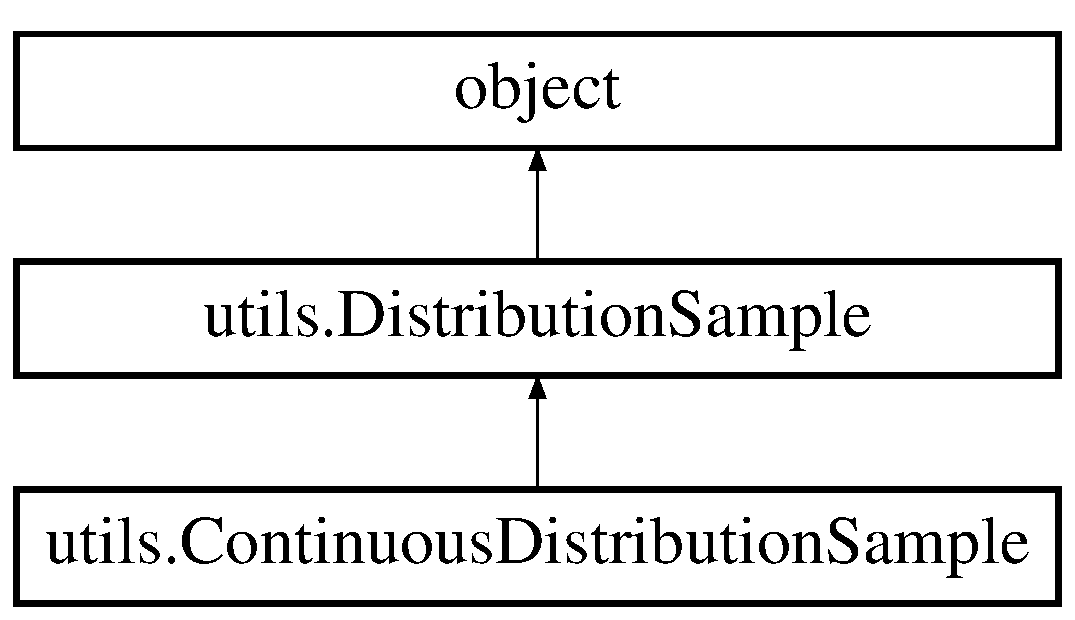
\includegraphics[height=3.000000cm]{classutils_1_1ContinuousDistributionSample}
\end{center}
\end{figure}
\subsubsection*{Public Member Functions}
\begin{DoxyCompactItemize}
\item 
def \hyperlink{classutils_1_1ContinuousDistributionSample_ac029b6c47f3f44850897aea5b1fcbaad}{\-\_\-\-\_\-init\-\_\-\-\_\-}
\item 
def \hyperlink{classutils_1_1ContinuousDistributionSample_a5741ea080eee2dd9c4ea26095788a621}{mean}
\item 
def \hyperlink{classutils_1_1ContinuousDistributionSample_aa45afba3caa9a3ca1b5b7f1eee18039d}{var}
\item 
def \hyperlink{classutils_1_1ContinuousDistributionSample_a85ecd7becac4ad7397c4cf870b33a6af}{reference\-Counts}
\item 
def \hyperlink{classutils_1_1ContinuousDistributionSample_a8cbbe383c9a0239b10fb1286b1d5db9f}{print\-Reference\-Counts}
\end{DoxyCompactItemize}
\subsubsection*{Static Public Member Functions}
\begin{DoxyCompactItemize}
\item 
def \hyperlink{classutils_1_1ContinuousDistributionSample_a3f0e197f9e7b0181dcdfaae7095f7a3f}{generate}
\end{DoxyCompactItemize}
\subsubsection*{Public Attributes}
\begin{DoxyCompactItemize}
\item 
\hyperlink{classutils_1_1ContinuousDistributionSample_a30f9569f79b47036e98571736411ab88}{categories}
\item 
\hyperlink{classutils_1_1ContinuousDistributionSample_aa339766ff21ac7752811c9a88f9338aa}{counts}
\end{DoxyCompactItemize}


\subsubsection{Detailed Description}
\begin{DoxyVerb}Class to represent a sample of a distribution for a continuous random variable
with the number of observations for each interval
intervals (categories variable) are defined by their left limits, the last one being the right limit
categories contain therefore one more element than the counts\end{DoxyVerb}
 

\subsubsection{Constructor \& Destructor Documentation}
\hypertarget{classutils_1_1ContinuousDistributionSample_ac029b6c47f3f44850897aea5b1fcbaad}{\index{utils\-::\-Continuous\-Distribution\-Sample@{utils\-::\-Continuous\-Distribution\-Sample}!\-\_\-\-\_\-init\-\_\-\-\_\-@{\-\_\-\-\_\-init\-\_\-\-\_\-}}
\index{\-\_\-\-\_\-init\-\_\-\-\_\-@{\-\_\-\-\_\-init\-\_\-\-\_\-}!utils::ContinuousDistributionSample@{utils\-::\-Continuous\-Distribution\-Sample}}
\paragraph[{\-\_\-\-\_\-init\-\_\-\-\_\-}]{\setlength{\rightskip}{0pt plus 5cm}def utils.\-Continuous\-Distribution\-Sample.\-\_\-\-\_\-init\-\_\-\-\_\- (
\begin{DoxyParamCaption}
\item[{}]{self, }
\item[{}]{categories, }
\item[{}]{counts}
\end{DoxyParamCaption}
)}}\label{classutils_1_1ContinuousDistributionSample_ac029b6c47f3f44850897aea5b1fcbaad}


\subsubsection{Member Function Documentation}
\hypertarget{classutils_1_1ContinuousDistributionSample_a3f0e197f9e7b0181dcdfaae7095f7a3f}{\index{utils\-::\-Continuous\-Distribution\-Sample@{utils\-::\-Continuous\-Distribution\-Sample}!generate@{generate}}
\index{generate@{generate}!utils::ContinuousDistributionSample@{utils\-::\-Continuous\-Distribution\-Sample}}
\paragraph[{generate}]{\setlength{\rightskip}{0pt plus 5cm}def utils.\-Continuous\-Distribution\-Sample.\-generate (
\begin{DoxyParamCaption}
\item[{}]{sample, }
\item[{}]{categories}
\end{DoxyParamCaption}
)\hspace{0.3cm}{\ttfamily [static]}}}\label{classutils_1_1ContinuousDistributionSample_a3f0e197f9e7b0181dcdfaae7095f7a3f}
\hypertarget{classutils_1_1ContinuousDistributionSample_a5741ea080eee2dd9c4ea26095788a621}{\index{utils\-::\-Continuous\-Distribution\-Sample@{utils\-::\-Continuous\-Distribution\-Sample}!mean@{mean}}
\index{mean@{mean}!utils::ContinuousDistributionSample@{utils\-::\-Continuous\-Distribution\-Sample}}
\paragraph[{mean}]{\setlength{\rightskip}{0pt plus 5cm}def utils.\-Continuous\-Distribution\-Sample.\-mean (
\begin{DoxyParamCaption}
\item[{}]{self}
\end{DoxyParamCaption}
)}}\label{classutils_1_1ContinuousDistributionSample_a5741ea080eee2dd9c4ea26095788a621}


References events.\-Interaction.\-categories, utils.\-Discrete\-Distribution\-Sample.\-categories, utils.\-Continuous\-Distribution\-Sample.\-categories, utils.\-Discrete\-Distribution\-Sample.\-counts, utils.\-Continuous\-Distribution\-Sample.\-counts, and utils.\-Distribution\-Sample.\-n\-Samples().

\hypertarget{classutils_1_1ContinuousDistributionSample_a8cbbe383c9a0239b10fb1286b1d5db9f}{\index{utils\-::\-Continuous\-Distribution\-Sample@{utils\-::\-Continuous\-Distribution\-Sample}!print\-Reference\-Counts@{print\-Reference\-Counts}}
\index{print\-Reference\-Counts@{print\-Reference\-Counts}!utils::ContinuousDistributionSample@{utils\-::\-Continuous\-Distribution\-Sample}}
\paragraph[{print\-Reference\-Counts}]{\setlength{\rightskip}{0pt plus 5cm}def utils.\-Continuous\-Distribution\-Sample.\-print\-Reference\-Counts (
\begin{DoxyParamCaption}
\item[{}]{self, }
\item[{}]{ref\-Counts = {\ttfamily None}}
\end{DoxyParamCaption}
)}}\label{classutils_1_1ContinuousDistributionSample_a8cbbe383c9a0239b10fb1286b1d5db9f}


References events.\-Interaction.\-categories, utils.\-Discrete\-Distribution\-Sample.\-categories, utils.\-Continuous\-Distribution\-Sample.\-categories, utils.\-Discrete\-Distribution\-Sample.\-reference\-Counts(), and utils.\-Continuous\-Distribution\-Sample.\-reference\-Counts().

\hypertarget{classutils_1_1ContinuousDistributionSample_a85ecd7becac4ad7397c4cf870b33a6af}{\index{utils\-::\-Continuous\-Distribution\-Sample@{utils\-::\-Continuous\-Distribution\-Sample}!reference\-Counts@{reference\-Counts}}
\index{reference\-Counts@{reference\-Counts}!utils::ContinuousDistributionSample@{utils\-::\-Continuous\-Distribution\-Sample}}
\paragraph[{reference\-Counts}]{\setlength{\rightskip}{0pt plus 5cm}def utils.\-Continuous\-Distribution\-Sample.\-reference\-Counts (
\begin{DoxyParamCaption}
\item[{}]{self, }
\item[{}]{cdf}
\end{DoxyParamCaption}
)}}\label{classutils_1_1ContinuousDistributionSample_a85ecd7becac4ad7397c4cf870b33a6af}
\begin{DoxyVerb}cdf is a cumulative distribution function
returning the probability of the variable being less that x\end{DoxyVerb}
 

References events.\-Interaction.\-categories, utils.\-Discrete\-Distribution\-Sample.\-categories, utils.\-Continuous\-Distribution\-Sample.\-categories, and utils.\-Distribution\-Sample.\-n\-Samples().

\hypertarget{classutils_1_1ContinuousDistributionSample_aa45afba3caa9a3ca1b5b7f1eee18039d}{\index{utils\-::\-Continuous\-Distribution\-Sample@{utils\-::\-Continuous\-Distribution\-Sample}!var@{var}}
\index{var@{var}!utils::ContinuousDistributionSample@{utils\-::\-Continuous\-Distribution\-Sample}}
\paragraph[{var}]{\setlength{\rightskip}{0pt plus 5cm}def utils.\-Continuous\-Distribution\-Sample.\-var (
\begin{DoxyParamCaption}
\item[{}]{self, }
\item[{}]{mean = {\ttfamily None}}
\end{DoxyParamCaption}
)}}\label{classutils_1_1ContinuousDistributionSample_aa45afba3caa9a3ca1b5b7f1eee18039d}


References events.\-Interaction.\-categories, utils.\-Discrete\-Distribution\-Sample.\-categories, utils.\-Continuous\-Distribution\-Sample.\-categories, utils.\-Discrete\-Distribution\-Sample.\-counts, utils.\-Continuous\-Distribution\-Sample.\-counts, utils.\-Discrete\-Distribution\-Sample.\-mean(), utils.\-Continuous\-Distribution\-Sample.\-mean(), and utils.\-Distribution\-Sample.\-n\-Samples().



\subsubsection{Member Data Documentation}
\hypertarget{classutils_1_1ContinuousDistributionSample_a30f9569f79b47036e98571736411ab88}{\index{utils\-::\-Continuous\-Distribution\-Sample@{utils\-::\-Continuous\-Distribution\-Sample}!categories@{categories}}
\index{categories@{categories}!utils::ContinuousDistributionSample@{utils\-::\-Continuous\-Distribution\-Sample}}
\paragraph[{categories}]{\setlength{\rightskip}{0pt plus 5cm}utils.\-Continuous\-Distribution\-Sample.\-categories}}\label{classutils_1_1ContinuousDistributionSample_a30f9569f79b47036e98571736411ab88}
\hypertarget{classutils_1_1ContinuousDistributionSample_aa339766ff21ac7752811c9a88f9338aa}{\index{utils\-::\-Continuous\-Distribution\-Sample@{utils\-::\-Continuous\-Distribution\-Sample}!counts@{counts}}
\index{counts@{counts}!utils::ContinuousDistributionSample@{utils\-::\-Continuous\-Distribution\-Sample}}
\paragraph[{counts}]{\setlength{\rightskip}{0pt plus 5cm}utils.\-Continuous\-Distribution\-Sample.\-counts}}\label{classutils_1_1ContinuousDistributionSample_aa339766ff21ac7752811c9a88f9338aa}


The documentation for this class was generated from the following file\-:\begin{DoxyCompactItemize}
\item 
python/\hyperlink{utils_8py}{utils.\-py}\end{DoxyCompactItemize}

\hypertarget{structCatch_1_1Counts}{\subsection{Catch\-:\-:Counts Struct Reference}
\label{structCatch_1_1Counts}\index{Catch\-::\-Counts@{Catch\-::\-Counts}}
}


{\ttfamily \#include $<$catch.\-hpp$>$}

\subsubsection*{Public Member Functions}
\begin{DoxyCompactItemize}
\item 
\hyperlink{structCatch_1_1Counts_aab9092ce70d4b0179cc743555d2fc39b}{Counts} ()
\item 
\hyperlink{structCatch_1_1Counts}{Counts} \hyperlink{structCatch_1_1Counts_a44035ac5faae026c24c61467ce49e501}{operator-\/} (const \hyperlink{structCatch_1_1Counts}{Counts} \&other) const 
\item 
\hyperlink{structCatch_1_1Counts}{Counts} \& \hyperlink{structCatch_1_1Counts_a727c114e105e44562554aecddea96cbb}{operator+=} (const \hyperlink{structCatch_1_1Counts}{Counts} \&other)
\item 
std\-::size\-\_\-t \hyperlink{structCatch_1_1Counts_a9125c662e30114e5c5cc94729b1e9e84}{total} () const 
\end{DoxyCompactItemize}
\subsubsection*{Public Attributes}
\begin{DoxyCompactItemize}
\item 
std\-::size\-\_\-t \hyperlink{structCatch_1_1Counts_ad28daaf3de28006400208b6dd0c631e6}{passed}
\item 
std\-::size\-\_\-t \hyperlink{structCatch_1_1Counts_a19982a3817a3bc2c07f0290e71f497a3}{failed}
\end{DoxyCompactItemize}


\subsubsection{Constructor \& Destructor Documentation}
\hypertarget{structCatch_1_1Counts_aab9092ce70d4b0179cc743555d2fc39b}{\index{Catch\-::\-Counts@{Catch\-::\-Counts}!Counts@{Counts}}
\index{Counts@{Counts}!Catch::Counts@{Catch\-::\-Counts}}
\paragraph[{Counts}]{\setlength{\rightskip}{0pt plus 5cm}Catch\-::\-Counts\-::\-Counts (
\begin{DoxyParamCaption}
{}
\end{DoxyParamCaption}
)\hspace{0.3cm}{\ttfamily [inline]}}}\label{structCatch_1_1Counts_aab9092ce70d4b0179cc743555d2fc39b}


\subsubsection{Member Function Documentation}
\hypertarget{structCatch_1_1Counts_a727c114e105e44562554aecddea96cbb}{\index{Catch\-::\-Counts@{Catch\-::\-Counts}!operator+=@{operator+=}}
\index{operator+=@{operator+=}!Catch::Counts@{Catch\-::\-Counts}}
\paragraph[{operator+=}]{\setlength{\rightskip}{0pt plus 5cm}{\bf Counts}\& Catch\-::\-Counts\-::operator+= (
\begin{DoxyParamCaption}
\item[{const {\bf Counts} \&}]{other}
\end{DoxyParamCaption}
)\hspace{0.3cm}{\ttfamily [inline]}}}\label{structCatch_1_1Counts_a727c114e105e44562554aecddea96cbb}


References failed, and passed.

\hypertarget{structCatch_1_1Counts_a44035ac5faae026c24c61467ce49e501}{\index{Catch\-::\-Counts@{Catch\-::\-Counts}!operator-\/@{operator-\/}}
\index{operator-\/@{operator-\/}!Catch::Counts@{Catch\-::\-Counts}}
\paragraph[{operator-\/}]{\setlength{\rightskip}{0pt plus 5cm}{\bf Counts} Catch\-::\-Counts\-::operator-\/ (
\begin{DoxyParamCaption}
\item[{const {\bf Counts} \&}]{other}
\end{DoxyParamCaption}
) const\hspace{0.3cm}{\ttfamily [inline]}}}\label{structCatch_1_1Counts_a44035ac5faae026c24c61467ce49e501}


References failed, and passed.

\hypertarget{structCatch_1_1Counts_a9125c662e30114e5c5cc94729b1e9e84}{\index{Catch\-::\-Counts@{Catch\-::\-Counts}!total@{total}}
\index{total@{total}!Catch::Counts@{Catch\-::\-Counts}}
\paragraph[{total}]{\setlength{\rightskip}{0pt plus 5cm}std\-::size\-\_\-t Catch\-::\-Counts\-::total (
\begin{DoxyParamCaption}
{}
\end{DoxyParamCaption}
) const\hspace{0.3cm}{\ttfamily [inline]}}}\label{structCatch_1_1Counts_a9125c662e30114e5c5cc94729b1e9e84}


References failed, and passed.



\subsubsection{Member Data Documentation}
\hypertarget{structCatch_1_1Counts_a19982a3817a3bc2c07f0290e71f497a3}{\index{Catch\-::\-Counts@{Catch\-::\-Counts}!failed@{failed}}
\index{failed@{failed}!Catch::Counts@{Catch\-::\-Counts}}
\paragraph[{failed}]{\setlength{\rightskip}{0pt plus 5cm}std\-::size\-\_\-t Catch\-::\-Counts\-::failed}}\label{structCatch_1_1Counts_a19982a3817a3bc2c07f0290e71f497a3}
\hypertarget{structCatch_1_1Counts_ad28daaf3de28006400208b6dd0c631e6}{\index{Catch\-::\-Counts@{Catch\-::\-Counts}!passed@{passed}}
\index{passed@{passed}!Catch::Counts@{Catch\-::\-Counts}}
\paragraph[{passed}]{\setlength{\rightskip}{0pt plus 5cm}std\-::size\-\_\-t Catch\-::\-Counts\-::passed}}\label{structCatch_1_1Counts_ad28daaf3de28006400208b6dd0c631e6}


The documentation for this struct was generated from the following file\-:\begin{DoxyCompactItemize}
\item 
include/\hyperlink{catch_8hpp}{catch.\-hpp}\end{DoxyCompactItemize}

\hypertarget{classevents_1_1Crossing}{\subsection{events.\-Crossing Class Reference}
\label{classevents_1_1Crossing}\index{events.\-Crossing@{events.\-Crossing}}
}
Inheritance diagram for events.\-Crossing\-:\begin{figure}[H]
\begin{center}
\leavevmode
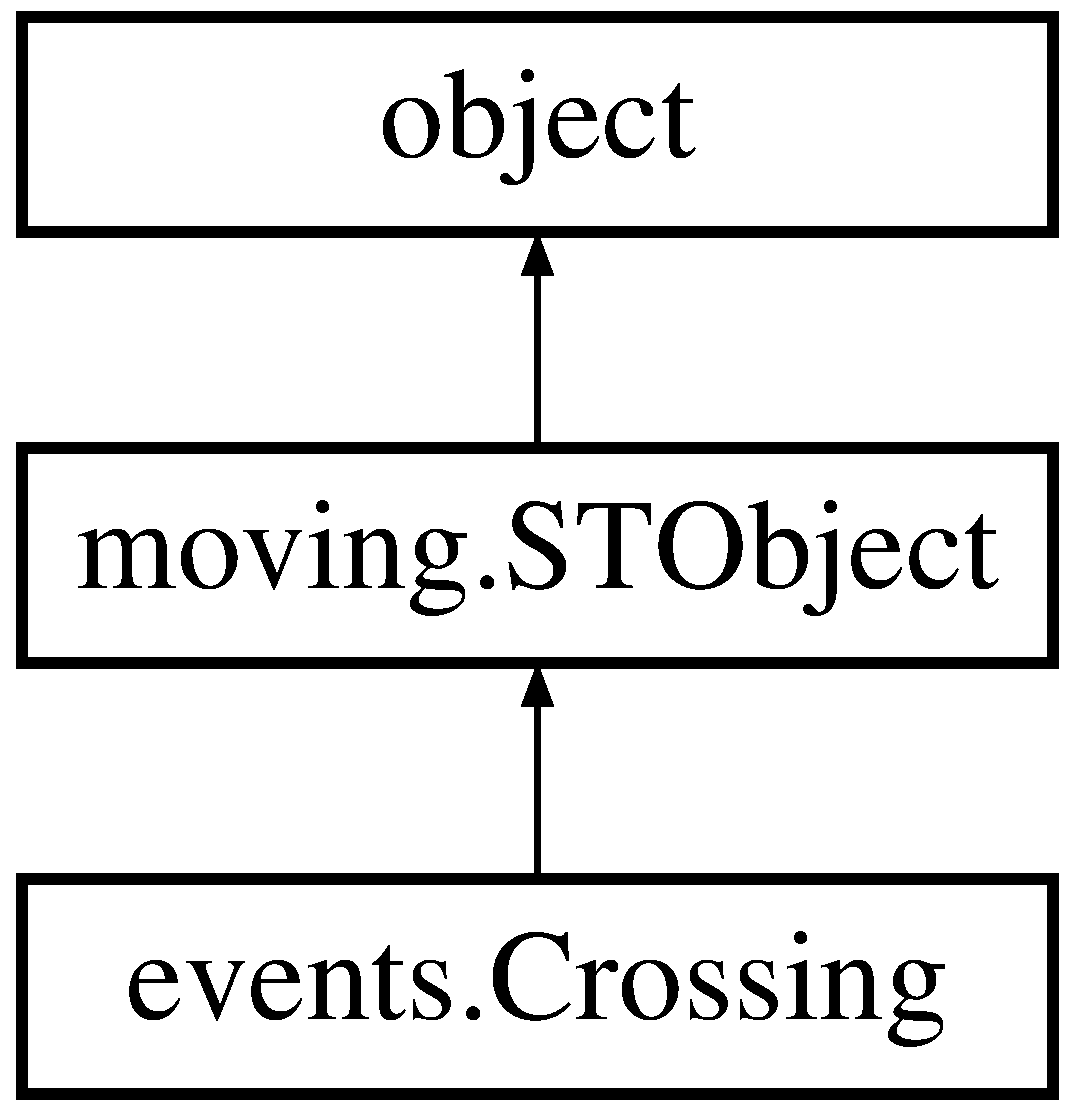
\includegraphics[height=3.000000cm]{classevents_1_1Crossing}
\end{center}
\end{figure}
\subsubsection*{Public Member Functions}
\begin{DoxyCompactItemize}
\item 
def \hyperlink{classevents_1_1Crossing_a427a80cea52ac4e21c83f04874ab1aad}{\-\_\-\-\_\-init\-\_\-\-\_\-}
\end{DoxyCompactItemize}
\subsubsection*{Public Attributes}
\begin{DoxyCompactItemize}
\item 
\hyperlink{classevents_1_1Crossing_a9d2107493a5c79aa7e3556eade66bf1a}{roaduser\-Num}
\end{DoxyCompactItemize}


\subsubsection{Detailed Description}
\begin{DoxyVerb}Class for the event of a street crossing

TODO: detecter passage sur la chaussee
identifier origines et destination (ou uniquement chaussee dans FOV)
carac traversee
detecter proximite veh (retirer si trop similaire simultanement
carac interaction\end{DoxyVerb}
 

\subsubsection{Constructor \& Destructor Documentation}
\hypertarget{classevents_1_1Crossing_a427a80cea52ac4e21c83f04874ab1aad}{\index{events\-::\-Crossing@{events\-::\-Crossing}!\-\_\-\-\_\-init\-\_\-\-\_\-@{\-\_\-\-\_\-init\-\_\-\-\_\-}}
\index{\-\_\-\-\_\-init\-\_\-\-\_\-@{\-\_\-\-\_\-init\-\_\-\-\_\-}!events::Crossing@{events\-::\-Crossing}}
\paragraph[{\-\_\-\-\_\-init\-\_\-\-\_\-}]{\setlength{\rightskip}{0pt plus 5cm}def events.\-Crossing.\-\_\-\-\_\-init\-\_\-\-\_\- (
\begin{DoxyParamCaption}
\item[{}]{self, }
\item[{}]{roaduser\-Num = {\ttfamily None}, }
\item[{}]{num = {\ttfamily None}, }
\item[{}]{time\-Interval = {\ttfamily None}}
\end{DoxyParamCaption}
)}}\label{classevents_1_1Crossing_a427a80cea52ac4e21c83f04874ab1aad}


References moving.\-S\-T\-Object.\-\_\-\-\_\-init\-\_\-\-\_\-().



\subsubsection{Member Data Documentation}
\hypertarget{classevents_1_1Crossing_a9d2107493a5c79aa7e3556eade66bf1a}{\index{events\-::\-Crossing@{events\-::\-Crossing}!roaduser\-Num@{roaduser\-Num}}
\index{roaduser\-Num@{roaduser\-Num}!events::Crossing@{events\-::\-Crossing}}
\paragraph[{roaduser\-Num}]{\setlength{\rightskip}{0pt plus 5cm}events.\-Crossing.\-roaduser\-Num}}\label{classevents_1_1Crossing_a9d2107493a5c79aa7e3556eade66bf1a}


The documentation for this class was generated from the following file\-:\begin{DoxyCompactItemize}
\item 
python/\hyperlink{events_8py}{events.\-py}\end{DoxyCompactItemize}

\hypertarget{classmoving_1_1CurvilinearTrajectory}{\subsection{moving.\-Curvilinear\-Trajectory Class Reference}
\label{classmoving_1_1CurvilinearTrajectory}\index{moving.\-Curvilinear\-Trajectory@{moving.\-Curvilinear\-Trajectory}}
}
Inheritance diagram for moving.\-Curvilinear\-Trajectory\-:\begin{figure}[H]
\begin{center}
\leavevmode
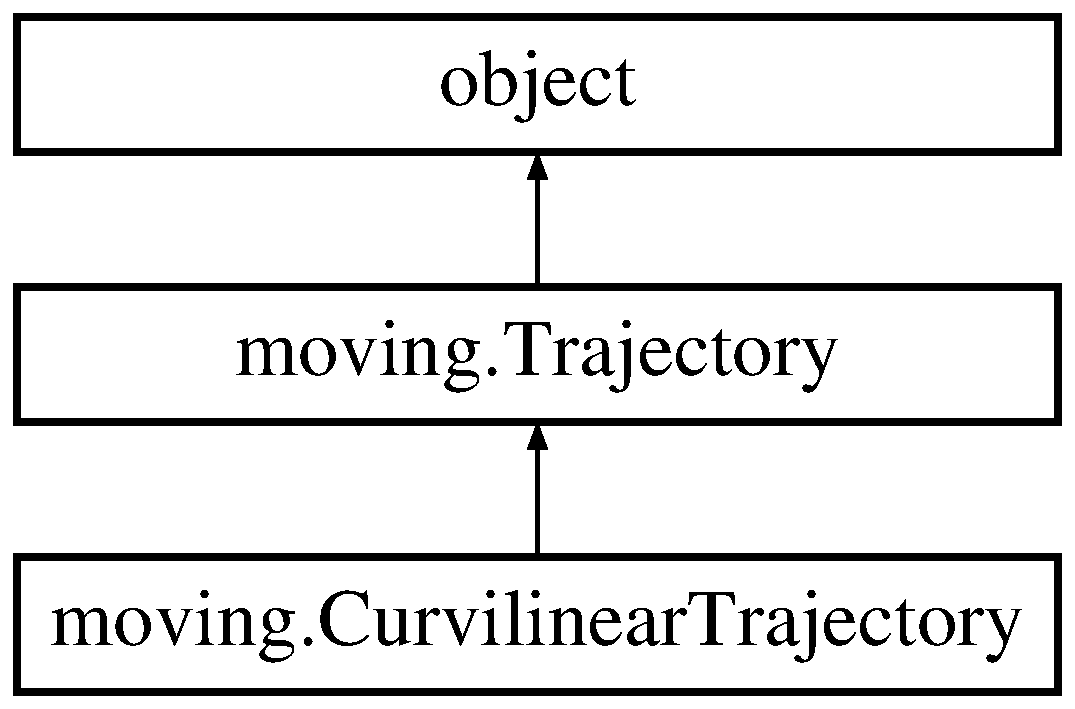
\includegraphics[height=3.000000cm]{classmoving_1_1CurvilinearTrajectory}
\end{center}
\end{figure}
\subsubsection*{Public Member Functions}
\begin{DoxyCompactItemize}
\item 
def \hyperlink{classmoving_1_1CurvilinearTrajectory_a9dbb459599ba451e5db49ba8692ef16e}{\-\_\-\-\_\-init\-\_\-\-\_\-}
\item 
def \hyperlink{classmoving_1_1CurvilinearTrajectory_afba688382acd78d1dbd754aa2359d7b2}{\-\_\-\-\_\-getitem\-\_\-\-\_\-}
\item 
def \hyperlink{classmoving_1_1CurvilinearTrajectory_a98a28cc819b039770d91d6cd85b07a9a}{get\-S\-Coordinates}
\item 
def \hyperlink{classmoving_1_1CurvilinearTrajectory_ae888b40fdc00f4709a941ba2f8347006}{get\-Lanes}
\item 
def \hyperlink{classmoving_1_1CurvilinearTrajectory_a99dd45bb2fb145ed4d870f526a7dc7fd}{add\-Position\-S\-Y\-L}
\item 
def \hyperlink{classmoving_1_1CurvilinearTrajectory_aac2115b52dc70976f439e6b218e1c2af}{add\-Position}
\item 
def \hyperlink{classmoving_1_1CurvilinearTrajectory_ad00be5c8422ea1f267f4f7938e306684}{set\-Position}
\item 
def \hyperlink{classmoving_1_1CurvilinearTrajectory_a09580b0a0713cb31cd3c5e82d7161a72}{differentiate}
\item 
def \hyperlink{classmoving_1_1CurvilinearTrajectory_a8dca85f2dd0c7d1ed7b40a2016b699c3}{get\-Intersections}
\end{DoxyCompactItemize}
\subsubsection*{Public Attributes}
\begin{DoxyCompactItemize}
\item 
\hyperlink{classmoving_1_1CurvilinearTrajectory_a165e6d95288f037dcdb94c04646d1952}{positions}
\item 
\hyperlink{classmoving_1_1CurvilinearTrajectory_a5ac59449b964d1a3907235bf6477ac52}{lanes}
\end{DoxyCompactItemize}
\subsubsection*{Additional Inherited Members}


\subsubsection{Detailed Description}
\begin{DoxyVerb}Sub class of trajectory for trajectories with curvilinear coordinates and lane assignements
longitudinal coordinate is stored as first coordinate (exterior name S)
lateral coordiante is stored as second coordinate\end{DoxyVerb}
 

\subsubsection{Constructor \& Destructor Documentation}
\hypertarget{classmoving_1_1CurvilinearTrajectory_a9dbb459599ba451e5db49ba8692ef16e}{\index{moving\-::\-Curvilinear\-Trajectory@{moving\-::\-Curvilinear\-Trajectory}!\-\_\-\-\_\-init\-\_\-\-\_\-@{\-\_\-\-\_\-init\-\_\-\-\_\-}}
\index{\-\_\-\-\_\-init\-\_\-\-\_\-@{\-\_\-\-\_\-init\-\_\-\-\_\-}!moving::CurvilinearTrajectory@{moving\-::\-Curvilinear\-Trajectory}}
\paragraph[{\-\_\-\-\_\-init\-\_\-\-\_\-}]{\setlength{\rightskip}{0pt plus 5cm}def moving.\-Curvilinear\-Trajectory.\-\_\-\-\_\-init\-\_\-\-\_\- (
\begin{DoxyParamCaption}
\item[{}]{self, }
\item[{}]{S = {\ttfamily None}, }
\item[{}]{Y = {\ttfamily None}, }
\item[{}]{lanes = {\ttfamily None}}
\end{DoxyParamCaption}
)}}\label{classmoving_1_1CurvilinearTrajectory_a9dbb459599ba451e5db49ba8692ef16e}


\subsubsection{Member Function Documentation}
\hypertarget{classmoving_1_1CurvilinearTrajectory_afba688382acd78d1dbd754aa2359d7b2}{\index{moving\-::\-Curvilinear\-Trajectory@{moving\-::\-Curvilinear\-Trajectory}!\-\_\-\-\_\-getitem\-\_\-\-\_\-@{\-\_\-\-\_\-getitem\-\_\-\-\_\-}}
\index{\-\_\-\-\_\-getitem\-\_\-\-\_\-@{\-\_\-\-\_\-getitem\-\_\-\-\_\-}!moving::CurvilinearTrajectory@{moving\-::\-Curvilinear\-Trajectory}}
\paragraph[{\-\_\-\-\_\-getitem\-\_\-\-\_\-}]{\setlength{\rightskip}{0pt plus 5cm}def moving.\-Curvilinear\-Trajectory.\-\_\-\-\_\-getitem\-\_\-\-\_\- (
\begin{DoxyParamCaption}
\item[{}]{self, }
\item[{}]{i}
\end{DoxyParamCaption}
)}}\label{classmoving_1_1CurvilinearTrajectory_afba688382acd78d1dbd754aa2359d7b2}


References moving.\-Curvilinear\-Trajectory.\-lanes, Feature\-Trajectory.\-positions, and moving.\-Trajectory.\-positions.

\hypertarget{classmoving_1_1CurvilinearTrajectory_aac2115b52dc70976f439e6b218e1c2af}{\index{moving\-::\-Curvilinear\-Trajectory@{moving\-::\-Curvilinear\-Trajectory}!add\-Position@{add\-Position}}
\index{add\-Position@{add\-Position}!moving::CurvilinearTrajectory@{moving\-::\-Curvilinear\-Trajectory}}
\paragraph[{add\-Position}]{\setlength{\rightskip}{0pt plus 5cm}def moving.\-Curvilinear\-Trajectory.\-add\-Position (
\begin{DoxyParamCaption}
\item[{}]{self, }
\item[{}]{p}
\end{DoxyParamCaption}
)}}\label{classmoving_1_1CurvilinearTrajectory_aac2115b52dc70976f439e6b218e1c2af}


References moving.\-Curvilinear\-Trajectory.\-add\-Position\-S\-Y\-L().

\hypertarget{classmoving_1_1CurvilinearTrajectory_a99dd45bb2fb145ed4d870f526a7dc7fd}{\index{moving\-::\-Curvilinear\-Trajectory@{moving\-::\-Curvilinear\-Trajectory}!add\-Position\-S\-Y\-L@{add\-Position\-S\-Y\-L}}
\index{add\-Position\-S\-Y\-L@{add\-Position\-S\-Y\-L}!moving::CurvilinearTrajectory@{moving\-::\-Curvilinear\-Trajectory}}
\paragraph[{add\-Position\-S\-Y\-L}]{\setlength{\rightskip}{0pt plus 5cm}def moving.\-Curvilinear\-Trajectory.\-add\-Position\-S\-Y\-L (
\begin{DoxyParamCaption}
\item[{}]{self, }
\item[{}]{s, }
\item[{}]{y, }
\item[{}]{lane}
\end{DoxyParamCaption}
)}}\label{classmoving_1_1CurvilinearTrajectory_a99dd45bb2fb145ed4d870f526a7dc7fd}


References moving.\-Trajectory.\-add\-Position\-X\-Y().

\hypertarget{classmoving_1_1CurvilinearTrajectory_a09580b0a0713cb31cd3c5e82d7161a72}{\index{moving\-::\-Curvilinear\-Trajectory@{moving\-::\-Curvilinear\-Trajectory}!differentiate@{differentiate}}
\index{differentiate@{differentiate}!moving::CurvilinearTrajectory@{moving\-::\-Curvilinear\-Trajectory}}
\paragraph[{differentiate}]{\setlength{\rightskip}{0pt plus 5cm}def moving.\-Curvilinear\-Trajectory.\-differentiate (
\begin{DoxyParamCaption}
\item[{}]{self, }
\item[{}]{double\-Last\-Position = {\ttfamily False}}
\end{DoxyParamCaption}
)}}\label{classmoving_1_1CurvilinearTrajectory_a09580b0a0713cb31cd3c5e82d7161a72}


References Feature\-Trajectory.\-length(), moving.\-Interval.\-length(), moving.\-Time\-Interval.\-length(), moving.\-S\-T\-Object.\-length(), and moving.\-Trajectory.\-length().

\hypertarget{classmoving_1_1CurvilinearTrajectory_a8dca85f2dd0c7d1ed7b40a2016b699c3}{\index{moving\-::\-Curvilinear\-Trajectory@{moving\-::\-Curvilinear\-Trajectory}!get\-Intersections@{get\-Intersections}}
\index{get\-Intersections@{get\-Intersections}!moving::CurvilinearTrajectory@{moving\-::\-Curvilinear\-Trajectory}}
\paragraph[{get\-Intersections}]{\setlength{\rightskip}{0pt plus 5cm}def moving.\-Curvilinear\-Trajectory.\-get\-Intersections (
\begin{DoxyParamCaption}
\item[{}]{self, }
\item[{}]{S1, }
\item[{}]{lane = {\ttfamily None}}
\end{DoxyParamCaption}
)}}\label{classmoving_1_1CurvilinearTrajectory_a8dca85f2dd0c7d1ed7b40a2016b699c3}
\begin{DoxyVerb}Returns a list of the indices at which the trajectory 
goes past the curvilinear coordinate S1
(in provided lane if lane is not None)
the list is empty if there is no crossing\end{DoxyVerb}
 

References indicators.\-Temporal\-Indicator.\-\_\-\-\_\-getitem\-\_\-\-\_\-(), moving.\-Time\-Interval.\-\_\-\-\_\-getitem\-\_\-\-\_\-(), moving.\-Point.\-\_\-\-\_\-getitem\-\_\-\-\_\-(), moving.\-Trajectory.\-\_\-\-\_\-getitem\-\_\-\-\_\-(), moving.\-Curvilinear\-Trajectory.\-lanes, Feature\-Trajectory.\-length(), moving.\-Interval.\-length(), moving.\-Time\-Interval.\-length(), moving.\-S\-T\-Object.\-length(), and moving.\-Trajectory.\-length().

\hypertarget{classmoving_1_1CurvilinearTrajectory_ae888b40fdc00f4709a941ba2f8347006}{\index{moving\-::\-Curvilinear\-Trajectory@{moving\-::\-Curvilinear\-Trajectory}!get\-Lanes@{get\-Lanes}}
\index{get\-Lanes@{get\-Lanes}!moving::CurvilinearTrajectory@{moving\-::\-Curvilinear\-Trajectory}}
\paragraph[{get\-Lanes}]{\setlength{\rightskip}{0pt plus 5cm}def moving.\-Curvilinear\-Trajectory.\-get\-Lanes (
\begin{DoxyParamCaption}
\item[{}]{self}
\end{DoxyParamCaption}
)}}\label{classmoving_1_1CurvilinearTrajectory_ae888b40fdc00f4709a941ba2f8347006}


References moving.\-Curvilinear\-Trajectory.\-lanes.

\hypertarget{classmoving_1_1CurvilinearTrajectory_a98a28cc819b039770d91d6cd85b07a9a}{\index{moving\-::\-Curvilinear\-Trajectory@{moving\-::\-Curvilinear\-Trajectory}!get\-S\-Coordinates@{get\-S\-Coordinates}}
\index{get\-S\-Coordinates@{get\-S\-Coordinates}!moving::CurvilinearTrajectory@{moving\-::\-Curvilinear\-Trajectory}}
\paragraph[{get\-S\-Coordinates}]{\setlength{\rightskip}{0pt plus 5cm}def moving.\-Curvilinear\-Trajectory.\-get\-S\-Coordinates (
\begin{DoxyParamCaption}
\item[{}]{self}
\end{DoxyParamCaption}
)}}\label{classmoving_1_1CurvilinearTrajectory_a98a28cc819b039770d91d6cd85b07a9a}


References moving.\-Trajectory.\-get\-X\-Coordinates().

\hypertarget{classmoving_1_1CurvilinearTrajectory_ad00be5c8422ea1f267f4f7938e306684}{\index{moving\-::\-Curvilinear\-Trajectory@{moving\-::\-Curvilinear\-Trajectory}!set\-Position@{set\-Position}}
\index{set\-Position@{set\-Position}!moving::CurvilinearTrajectory@{moving\-::\-Curvilinear\-Trajectory}}
\paragraph[{set\-Position}]{\setlength{\rightskip}{0pt plus 5cm}def moving.\-Curvilinear\-Trajectory.\-set\-Position (
\begin{DoxyParamCaption}
\item[{}]{self, }
\item[{}]{i, }
\item[{}]{s, }
\item[{}]{y, }
\item[{}]{lane}
\end{DoxyParamCaption}
)}}\label{classmoving_1_1CurvilinearTrajectory_ad00be5c8422ea1f267f4f7938e306684}


References indicators.\-Temporal\-Indicator.\-\_\-\-\_\-len\-\_\-\-\_\-(), moving.\-Time\-Interval.\-\_\-\-\_\-len\-\_\-\-\_\-(), moving.\-S\-T\-Object.\-\_\-\-\_\-len\-\_\-\-\_\-(), moving.\-Trajectory.\-\_\-\-\_\-len\-\_\-\-\_\-(), moving.\-Curvilinear\-Trajectory.\-lanes, and moving.\-Trajectory.\-set\-Position\-X\-Y().



\subsubsection{Member Data Documentation}
\hypertarget{classmoving_1_1CurvilinearTrajectory_a5ac59449b964d1a3907235bf6477ac52}{\index{moving\-::\-Curvilinear\-Trajectory@{moving\-::\-Curvilinear\-Trajectory}!lanes@{lanes}}
\index{lanes@{lanes}!moving::CurvilinearTrajectory@{moving\-::\-Curvilinear\-Trajectory}}
\paragraph[{lanes}]{\setlength{\rightskip}{0pt plus 5cm}moving.\-Curvilinear\-Trajectory.\-lanes}}\label{classmoving_1_1CurvilinearTrajectory_a5ac59449b964d1a3907235bf6477ac52}
\hypertarget{classmoving_1_1CurvilinearTrajectory_a165e6d95288f037dcdb94c04646d1952}{\index{moving\-::\-Curvilinear\-Trajectory@{moving\-::\-Curvilinear\-Trajectory}!positions@{positions}}
\index{positions@{positions}!moving::CurvilinearTrajectory@{moving\-::\-Curvilinear\-Trajectory}}
\paragraph[{positions}]{\setlength{\rightskip}{0pt plus 5cm}moving.\-Curvilinear\-Trajectory.\-positions}}\label{classmoving_1_1CurvilinearTrajectory_a165e6d95288f037dcdb94c04646d1952}


The documentation for this class was generated from the following file\-:\begin{DoxyCompactItemize}
\item 
python/\hyperlink{moving_8py}{moving.\-py}\end{DoxyCompactItemize}

\hypertarget{classprediction_1_1CVDirectPredictionParameters}{\subsection{prediction.\-C\-V\-Direct\-Prediction\-Parameters Class Reference}
\label{classprediction_1_1CVDirectPredictionParameters}\index{prediction.\-C\-V\-Direct\-Prediction\-Parameters@{prediction.\-C\-V\-Direct\-Prediction\-Parameters}}
}
Inheritance diagram for prediction.\-C\-V\-Direct\-Prediction\-Parameters\-:\begin{figure}[H]
\begin{center}
\leavevmode
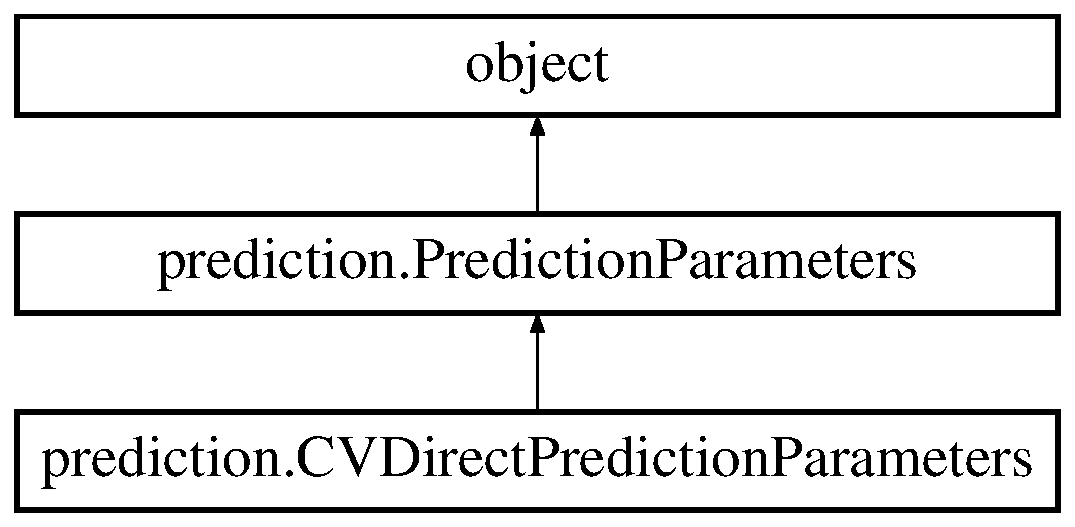
\includegraphics[height=3.000000cm]{classprediction_1_1CVDirectPredictionParameters}
\end{center}
\end{figure}
\subsubsection*{Public Member Functions}
\begin{DoxyCompactItemize}
\item 
def \hyperlink{classprediction_1_1CVDirectPredictionParameters_a0199b4a5f2c19e30285bc54033c015b3}{\-\_\-\-\_\-init\-\_\-\-\_\-}
\item 
def \hyperlink{classprediction_1_1CVDirectPredictionParameters_aacee8062dce9911dac3e148766a24dde}{compute\-Crossings\-Collisions\-At\-Instant}
\end{DoxyCompactItemize}
\subsubsection*{Additional Inherited Members}


\subsubsection{Detailed Description}
\begin{DoxyVerb}Prediction parameters of prediction at constant velocity
using direct computation of the intersecting point
Warning: the computed time to collision may be higher than timeHorizon (not used)\end{DoxyVerb}
 

\subsubsection{Constructor \& Destructor Documentation}
\hypertarget{classprediction_1_1CVDirectPredictionParameters_a0199b4a5f2c19e30285bc54033c015b3}{\index{prediction\-::\-C\-V\-Direct\-Prediction\-Parameters@{prediction\-::\-C\-V\-Direct\-Prediction\-Parameters}!\-\_\-\-\_\-init\-\_\-\-\_\-@{\-\_\-\-\_\-init\-\_\-\-\_\-}}
\index{\-\_\-\-\_\-init\-\_\-\-\_\-@{\-\_\-\-\_\-init\-\_\-\-\_\-}!prediction::CVDirectPredictionParameters@{prediction\-::\-C\-V\-Direct\-Prediction\-Parameters}}
\paragraph[{\-\_\-\-\_\-init\-\_\-\-\_\-}]{\setlength{\rightskip}{0pt plus 5cm}def prediction.\-C\-V\-Direct\-Prediction\-Parameters.\-\_\-\-\_\-init\-\_\-\-\_\- (
\begin{DoxyParamCaption}
\item[{}]{self}
\end{DoxyParamCaption}
)}}\label{classprediction_1_1CVDirectPredictionParameters_a0199b4a5f2c19e30285bc54033c015b3}


\subsubsection{Member Function Documentation}
\hypertarget{classprediction_1_1CVDirectPredictionParameters_aacee8062dce9911dac3e148766a24dde}{\index{prediction\-::\-C\-V\-Direct\-Prediction\-Parameters@{prediction\-::\-C\-V\-Direct\-Prediction\-Parameters}!compute\-Crossings\-Collisions\-At\-Instant@{compute\-Crossings\-Collisions\-At\-Instant}}
\index{compute\-Crossings\-Collisions\-At\-Instant@{compute\-Crossings\-Collisions\-At\-Instant}!prediction::CVDirectPredictionParameters@{prediction\-::\-C\-V\-Direct\-Prediction\-Parameters}}
\paragraph[{compute\-Crossings\-Collisions\-At\-Instant}]{\setlength{\rightskip}{0pt plus 5cm}def prediction.\-C\-V\-Direct\-Prediction\-Parameters.\-compute\-Crossings\-Collisions\-At\-Instant (
\begin{DoxyParamCaption}
\item[{}]{self, }
\item[{}]{current\-Instant, }
\item[{}]{obj1, }
\item[{}]{obj2, }
\item[{}]{collision\-Distance\-Threshold, }
\item[{}]{time\-Horizon, }
\item[{}]{compute\-C\-Z = {\ttfamily False}, }
\item[{}]{debug = {\ttfamily False}, }
\item[{}]{kwargs}
\end{DoxyParamCaption}
)}}\label{classprediction_1_1CVDirectPredictionParameters_aacee8062dce9911dac3e148766a24dde}


References moving.\-Point.\-dot(), moving.\-Interval.\-intersection(), and moving.\-intersection().



The documentation for this class was generated from the following file\-:\begin{DoxyCompactItemize}
\item 
python/\hyperlink{prediction_8py}{prediction.\-py}\end{DoxyCompactItemize}

\hypertarget{classprediction_1_1CVExactPredictionParameters}{\subsection{prediction.\-C\-V\-Exact\-Prediction\-Parameters Class Reference}
\label{classprediction_1_1CVExactPredictionParameters}\index{prediction.\-C\-V\-Exact\-Prediction\-Parameters@{prediction.\-C\-V\-Exact\-Prediction\-Parameters}}
}
Inheritance diagram for prediction.\-C\-V\-Exact\-Prediction\-Parameters\-:\begin{figure}[H]
\begin{center}
\leavevmode
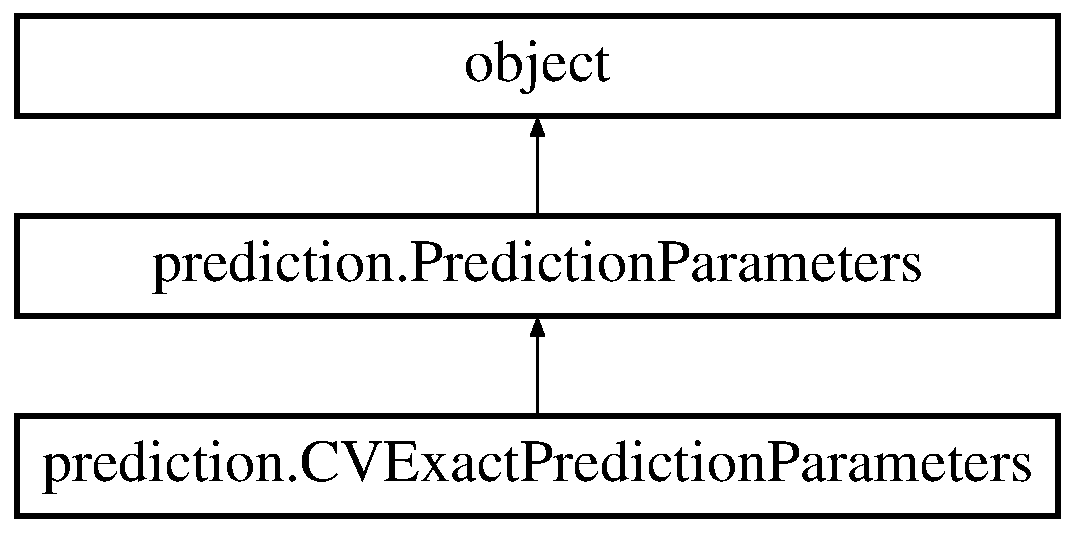
\includegraphics[height=3.000000cm]{classprediction_1_1CVExactPredictionParameters}
\end{center}
\end{figure}
\subsubsection*{Public Member Functions}
\begin{DoxyCompactItemize}
\item 
def \hyperlink{classprediction_1_1CVExactPredictionParameters_a5dcd0f68b0f3d183de4df10331594d9d}{\-\_\-\-\_\-init\-\_\-\-\_\-}
\item 
def \hyperlink{classprediction_1_1CVExactPredictionParameters_a28a2b07587dd6c5e6996948b04c7141c}{compute\-Crossings\-Collisions\-At\-Instant}
\end{DoxyCompactItemize}
\subsubsection*{Additional Inherited Members}


\subsubsection{Detailed Description}
\begin{DoxyVerb}Prediction parameters of prediction at constant velocity
using direct computation of the intersecting point (solving the equation)
Warning: the computed time to collision may be higher than timeHorizon (not used)\end{DoxyVerb}
 

\subsubsection{Constructor \& Destructor Documentation}
\hypertarget{classprediction_1_1CVExactPredictionParameters_a5dcd0f68b0f3d183de4df10331594d9d}{\index{prediction\-::\-C\-V\-Exact\-Prediction\-Parameters@{prediction\-::\-C\-V\-Exact\-Prediction\-Parameters}!\-\_\-\-\_\-init\-\_\-\-\_\-@{\-\_\-\-\_\-init\-\_\-\-\_\-}}
\index{\-\_\-\-\_\-init\-\_\-\-\_\-@{\-\_\-\-\_\-init\-\_\-\-\_\-}!prediction::CVExactPredictionParameters@{prediction\-::\-C\-V\-Exact\-Prediction\-Parameters}}
\paragraph[{\-\_\-\-\_\-init\-\_\-\-\_\-}]{\setlength{\rightskip}{0pt plus 5cm}def prediction.\-C\-V\-Exact\-Prediction\-Parameters.\-\_\-\-\_\-init\-\_\-\-\_\- (
\begin{DoxyParamCaption}
\item[{}]{self}
\end{DoxyParamCaption}
)}}\label{classprediction_1_1CVExactPredictionParameters_a5dcd0f68b0f3d183de4df10331594d9d}


\subsubsection{Member Function Documentation}
\hypertarget{classprediction_1_1CVExactPredictionParameters_a28a2b07587dd6c5e6996948b04c7141c}{\index{prediction\-::\-C\-V\-Exact\-Prediction\-Parameters@{prediction\-::\-C\-V\-Exact\-Prediction\-Parameters}!compute\-Crossings\-Collisions\-At\-Instant@{compute\-Crossings\-Collisions\-At\-Instant}}
\index{compute\-Crossings\-Collisions\-At\-Instant@{compute\-Crossings\-Collisions\-At\-Instant}!prediction::CVExactPredictionParameters@{prediction\-::\-C\-V\-Exact\-Prediction\-Parameters}}
\paragraph[{compute\-Crossings\-Collisions\-At\-Instant}]{\setlength{\rightskip}{0pt plus 5cm}def prediction.\-C\-V\-Exact\-Prediction\-Parameters.\-compute\-Crossings\-Collisions\-At\-Instant (
\begin{DoxyParamCaption}
\item[{}]{self, }
\item[{}]{current\-Instant, }
\item[{}]{obj1, }
\item[{}]{obj2, }
\item[{}]{collision\-Distance\-Threshold, }
\item[{}]{time\-Horizon, }
\item[{}]{compute\-C\-Z = {\ttfamily False}, }
\item[{}]{debug = {\ttfamily False}, }
\item[{}]{kwargs}
\end{DoxyParamCaption}
)}}\label{classprediction_1_1CVExactPredictionParameters_a28a2b07587dd6c5e6996948b04c7141c}


References moving.\-intersection(), and moving.\-Point.\-time\-To\-Collision().



The documentation for this class was generated from the following file\-:\begin{DoxyCompactItemize}
\item 
python/\hyperlink{prediction_8py}{prediction.\-py}\end{DoxyCompactItemize}

\hypertarget{classtraffic__engineering_1_1Cycle}{\subsection{traffic\-\_\-engineering.\-Cycle Class Reference}
\label{classtraffic__engineering_1_1Cycle}\index{traffic\-\_\-engineering.\-Cycle@{traffic\-\_\-engineering.\-Cycle}}
}
Inheritance diagram for traffic\-\_\-engineering.\-Cycle\-:\begin{figure}[H]
\begin{center}
\leavevmode
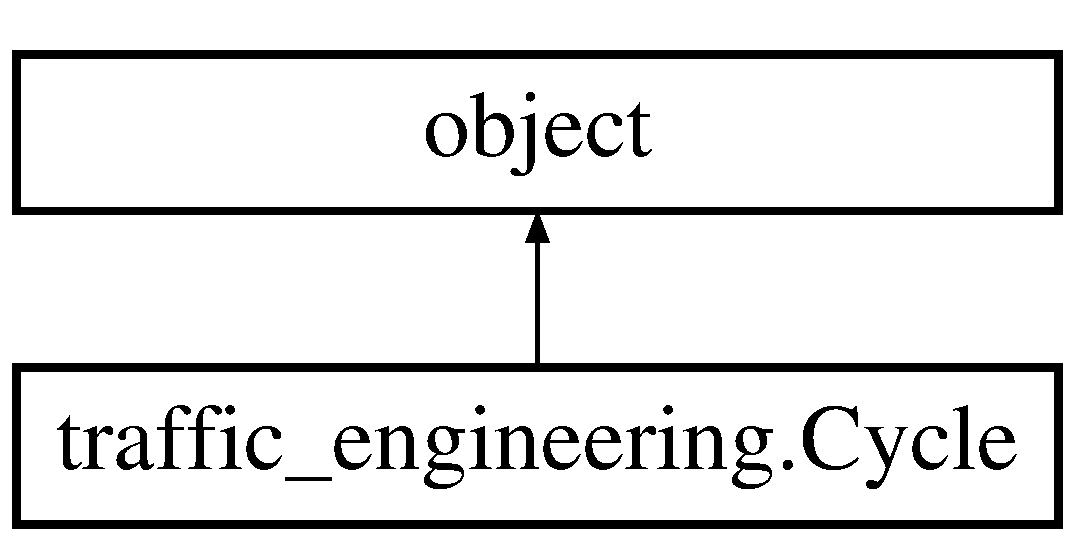
\includegraphics[height=2.000000cm]{classtraffic__engineering_1_1Cycle}
\end{center}
\end{figure}
\subsubsection*{Public Member Functions}
\begin{DoxyCompactItemize}
\item 
def \hyperlink{classtraffic__engineering_1_1Cycle_a0eeb478326b8bf89c5ee21ad358b9a1d}{\-\_\-\-\_\-init\-\_\-\-\_\-}
\item 
def \hyperlink{classtraffic__engineering_1_1Cycle_aa4d18da4fda77fcaf9e00dda517a9bcd}{compute\-Critical\-Charges}
\item 
def \hyperlink{classtraffic__engineering_1_1Cycle_a3dde9ca514dd8a334e124cf786d725a3}{compute\-Optimal\-Cycle}
\item 
def \hyperlink{classtraffic__engineering_1_1Cycle_a9c06b3bca0b5ae4d9679423fa8258d01}{compute\-Minimum\-Cycle}
\item 
def \hyperlink{classtraffic__engineering_1_1Cycle_ae139a083fc6f3fb86939056785d12183}{compute\-Effective\-Green}
\end{DoxyCompactItemize}
\subsubsection*{Public Attributes}
\begin{DoxyCompactItemize}
\item 
\hyperlink{classtraffic__engineering_1_1Cycle_a7202bcc832f21d2311dff51842fe3e36}{phases}
\item 
\hyperlink{classtraffic__engineering_1_1Cycle_a801a2abdd55ed7c9ed519b0abd10ef4d}{lost\-Time}
\item 
\hyperlink{classtraffic__engineering_1_1Cycle_a81c12a6440679f60ee65e414df5d5a19}{saturation\-Volume}
\item 
\hyperlink{classtraffic__engineering_1_1Cycle_a334243c820e2c15c9864402c8feeaf99}{critical\-Charges}
\item 
\hyperlink{classtraffic__engineering_1_1Cycle_af6c974b3131875856225881f371c8244}{critical\-Charge}
\item 
\hyperlink{classtraffic__engineering_1_1Cycle_a5f62eacf748d8b5628bb5836f75b54ec}{C}
\item 
\hyperlink{classtraffic__engineering_1_1Cycle_a3efbac462e3bb903e6657668b72f689b}{effective\-Greens}
\end{DoxyCompactItemize}


\subsubsection{Detailed Description}
\begin{DoxyVerb}Class to compute optimal cycle and the split of effective green times\end{DoxyVerb}
 

\subsubsection{Constructor \& Destructor Documentation}
\hypertarget{classtraffic__engineering_1_1Cycle_a0eeb478326b8bf89c5ee21ad358b9a1d}{\index{traffic\-\_\-engineering\-::\-Cycle@{traffic\-\_\-engineering\-::\-Cycle}!\-\_\-\-\_\-init\-\_\-\-\_\-@{\-\_\-\-\_\-init\-\_\-\-\_\-}}
\index{\-\_\-\-\_\-init\-\_\-\-\_\-@{\-\_\-\-\_\-init\-\_\-\-\_\-}!traffic_engineering::Cycle@{traffic\-\_\-engineering\-::\-Cycle}}
\paragraph[{\-\_\-\-\_\-init\-\_\-\-\_\-}]{\setlength{\rightskip}{0pt plus 5cm}def traffic\-\_\-engineering.\-Cycle.\-\_\-\-\_\-init\-\_\-\-\_\- (
\begin{DoxyParamCaption}
\item[{}]{self, }
\item[{}]{phases, }
\item[{}]{lost\-Time, }
\item[{}]{saturation\-Volume}
\end{DoxyParamCaption}
)}}\label{classtraffic__engineering_1_1Cycle_a0eeb478326b8bf89c5ee21ad358b9a1d}
\begin{DoxyVerb}phases is a list of phases
a phase is a list of lanegroups\end{DoxyVerb}
 

\subsubsection{Member Function Documentation}
\hypertarget{classtraffic__engineering_1_1Cycle_aa4d18da4fda77fcaf9e00dda517a9bcd}{\index{traffic\-\_\-engineering\-::\-Cycle@{traffic\-\_\-engineering\-::\-Cycle}!compute\-Critical\-Charges@{compute\-Critical\-Charges}}
\index{compute\-Critical\-Charges@{compute\-Critical\-Charges}!traffic_engineering::Cycle@{traffic\-\_\-engineering\-::\-Cycle}}
\paragraph[{compute\-Critical\-Charges}]{\setlength{\rightskip}{0pt plus 5cm}def traffic\-\_\-engineering.\-Cycle.\-compute\-Critical\-Charges (
\begin{DoxyParamCaption}
\item[{}]{self}
\end{DoxyParamCaption}
)}}\label{classtraffic__engineering_1_1Cycle_aa4d18da4fda77fcaf9e00dda517a9bcd}
\hypertarget{classtraffic__engineering_1_1Cycle_ae139a083fc6f3fb86939056785d12183}{\index{traffic\-\_\-engineering\-::\-Cycle@{traffic\-\_\-engineering\-::\-Cycle}!compute\-Effective\-Green@{compute\-Effective\-Green}}
\index{compute\-Effective\-Green@{compute\-Effective\-Green}!traffic_engineering::Cycle@{traffic\-\_\-engineering\-::\-Cycle}}
\paragraph[{compute\-Effective\-Green}]{\setlength{\rightskip}{0pt plus 5cm}def traffic\-\_\-engineering.\-Cycle.\-compute\-Effective\-Green (
\begin{DoxyParamCaption}
\item[{}]{self}
\end{DoxyParamCaption}
)}}\label{classtraffic__engineering_1_1Cycle_ae139a083fc6f3fb86939056785d12183}


References traffic\-\_\-engineering.\-Cycle.\-C, and traffic\-\_\-engineering.\-Cycle.\-lost\-Time.

\hypertarget{classtraffic__engineering_1_1Cycle_a9c06b3bca0b5ae4d9679423fa8258d01}{\index{traffic\-\_\-engineering\-::\-Cycle@{traffic\-\_\-engineering\-::\-Cycle}!compute\-Minimum\-Cycle@{compute\-Minimum\-Cycle}}
\index{compute\-Minimum\-Cycle@{compute\-Minimum\-Cycle}!traffic_engineering::Cycle@{traffic\-\_\-engineering\-::\-Cycle}}
\paragraph[{compute\-Minimum\-Cycle}]{\setlength{\rightskip}{0pt plus 5cm}def traffic\-\_\-engineering.\-Cycle.\-compute\-Minimum\-Cycle (
\begin{DoxyParamCaption}
\item[{}]{self, }
\item[{}]{degree\-Saturation = {\ttfamily 1.}}
\end{DoxyParamCaption}
)}}\label{classtraffic__engineering_1_1Cycle_a9c06b3bca0b5ae4d9679423fa8258d01}


References traffic\-\_\-engineering.\-Cycle.\-C, traffic\-\_\-engineering.\-Cycle.\-compute\-Critical\-Charges(), traffic\-\_\-engineering.\-Cycle.\-critical\-Charge, traffic\-\_\-engineering.\-Cycle.\-lost\-Time, and traffic\-\_\-engineering.\-minimum\-Cycle().

\hypertarget{classtraffic__engineering_1_1Cycle_a3dde9ca514dd8a334e124cf786d725a3}{\index{traffic\-\_\-engineering\-::\-Cycle@{traffic\-\_\-engineering\-::\-Cycle}!compute\-Optimal\-Cycle@{compute\-Optimal\-Cycle}}
\index{compute\-Optimal\-Cycle@{compute\-Optimal\-Cycle}!traffic_engineering::Cycle@{traffic\-\_\-engineering\-::\-Cycle}}
\paragraph[{compute\-Optimal\-Cycle}]{\setlength{\rightskip}{0pt plus 5cm}def traffic\-\_\-engineering.\-Cycle.\-compute\-Optimal\-Cycle (
\begin{DoxyParamCaption}
\item[{}]{self}
\end{DoxyParamCaption}
)}}\label{classtraffic__engineering_1_1Cycle_a3dde9ca514dd8a334e124cf786d725a3}


References traffic\-\_\-engineering.\-Cycle.\-compute\-Critical\-Charges().



\subsubsection{Member Data Documentation}
\hypertarget{classtraffic__engineering_1_1Cycle_a5f62eacf748d8b5628bb5836f75b54ec}{\index{traffic\-\_\-engineering\-::\-Cycle@{traffic\-\_\-engineering\-::\-Cycle}!C@{C}}
\index{C@{C}!traffic_engineering::Cycle@{traffic\-\_\-engineering\-::\-Cycle}}
\paragraph[{C}]{\setlength{\rightskip}{0pt plus 5cm}traffic\-\_\-engineering.\-Cycle.\-C}}\label{classtraffic__engineering_1_1Cycle_a5f62eacf748d8b5628bb5836f75b54ec}
\hypertarget{classtraffic__engineering_1_1Cycle_af6c974b3131875856225881f371c8244}{\index{traffic\-\_\-engineering\-::\-Cycle@{traffic\-\_\-engineering\-::\-Cycle}!critical\-Charge@{critical\-Charge}}
\index{critical\-Charge@{critical\-Charge}!traffic_engineering::Cycle@{traffic\-\_\-engineering\-::\-Cycle}}
\paragraph[{critical\-Charge}]{\setlength{\rightskip}{0pt plus 5cm}traffic\-\_\-engineering.\-Cycle.\-critical\-Charge}}\label{classtraffic__engineering_1_1Cycle_af6c974b3131875856225881f371c8244}
\hypertarget{classtraffic__engineering_1_1Cycle_a334243c820e2c15c9864402c8feeaf99}{\index{traffic\-\_\-engineering\-::\-Cycle@{traffic\-\_\-engineering\-::\-Cycle}!critical\-Charges@{critical\-Charges}}
\index{critical\-Charges@{critical\-Charges}!traffic_engineering::Cycle@{traffic\-\_\-engineering\-::\-Cycle}}
\paragraph[{critical\-Charges}]{\setlength{\rightskip}{0pt plus 5cm}traffic\-\_\-engineering.\-Cycle.\-critical\-Charges}}\label{classtraffic__engineering_1_1Cycle_a334243c820e2c15c9864402c8feeaf99}
\hypertarget{classtraffic__engineering_1_1Cycle_a3efbac462e3bb903e6657668b72f689b}{\index{traffic\-\_\-engineering\-::\-Cycle@{traffic\-\_\-engineering\-::\-Cycle}!effective\-Greens@{effective\-Greens}}
\index{effective\-Greens@{effective\-Greens}!traffic_engineering::Cycle@{traffic\-\_\-engineering\-::\-Cycle}}
\paragraph[{effective\-Greens}]{\setlength{\rightskip}{0pt plus 5cm}traffic\-\_\-engineering.\-Cycle.\-effective\-Greens}}\label{classtraffic__engineering_1_1Cycle_a3efbac462e3bb903e6657668b72f689b}
\hypertarget{classtraffic__engineering_1_1Cycle_a801a2abdd55ed7c9ed519b0abd10ef4d}{\index{traffic\-\_\-engineering\-::\-Cycle@{traffic\-\_\-engineering\-::\-Cycle}!lost\-Time@{lost\-Time}}
\index{lost\-Time@{lost\-Time}!traffic_engineering::Cycle@{traffic\-\_\-engineering\-::\-Cycle}}
\paragraph[{lost\-Time}]{\setlength{\rightskip}{0pt plus 5cm}traffic\-\_\-engineering.\-Cycle.\-lost\-Time}}\label{classtraffic__engineering_1_1Cycle_a801a2abdd55ed7c9ed519b0abd10ef4d}
\hypertarget{classtraffic__engineering_1_1Cycle_a7202bcc832f21d2311dff51842fe3e36}{\index{traffic\-\_\-engineering\-::\-Cycle@{traffic\-\_\-engineering\-::\-Cycle}!phases@{phases}}
\index{phases@{phases}!traffic_engineering::Cycle@{traffic\-\_\-engineering\-::\-Cycle}}
\paragraph[{phases}]{\setlength{\rightskip}{0pt plus 5cm}traffic\-\_\-engineering.\-Cycle.\-phases}}\label{classtraffic__engineering_1_1Cycle_a7202bcc832f21d2311dff51842fe3e36}
\hypertarget{classtraffic__engineering_1_1Cycle_a81c12a6440679f60ee65e414df5d5a19}{\index{traffic\-\_\-engineering\-::\-Cycle@{traffic\-\_\-engineering\-::\-Cycle}!saturation\-Volume@{saturation\-Volume}}
\index{saturation\-Volume@{saturation\-Volume}!traffic_engineering::Cycle@{traffic\-\_\-engineering\-::\-Cycle}}
\paragraph[{saturation\-Volume}]{\setlength{\rightskip}{0pt plus 5cm}traffic\-\_\-engineering.\-Cycle.\-saturation\-Volume}}\label{classtraffic__engineering_1_1Cycle_a81c12a6440679f60ee65e414df5d5a19}


The documentation for this class was generated from the following file\-:\begin{DoxyCompactItemize}
\item 
python/\hyperlink{traffic__engineering_8py}{traffic\-\_\-engineering.\-py}\end{DoxyCompactItemize}

\hypertarget{classtraffic__engineering_1_1Cyclist}{\subsection{traffic\-\_\-engineering.\-Cyclist Class Reference}
\label{classtraffic__engineering_1_1Cyclist}\index{traffic\-\_\-engineering.\-Cyclist@{traffic\-\_\-engineering.\-Cyclist}}
}
Inheritance diagram for traffic\-\_\-engineering.\-Cyclist\-:\begin{figure}[H]
\begin{center}
\leavevmode
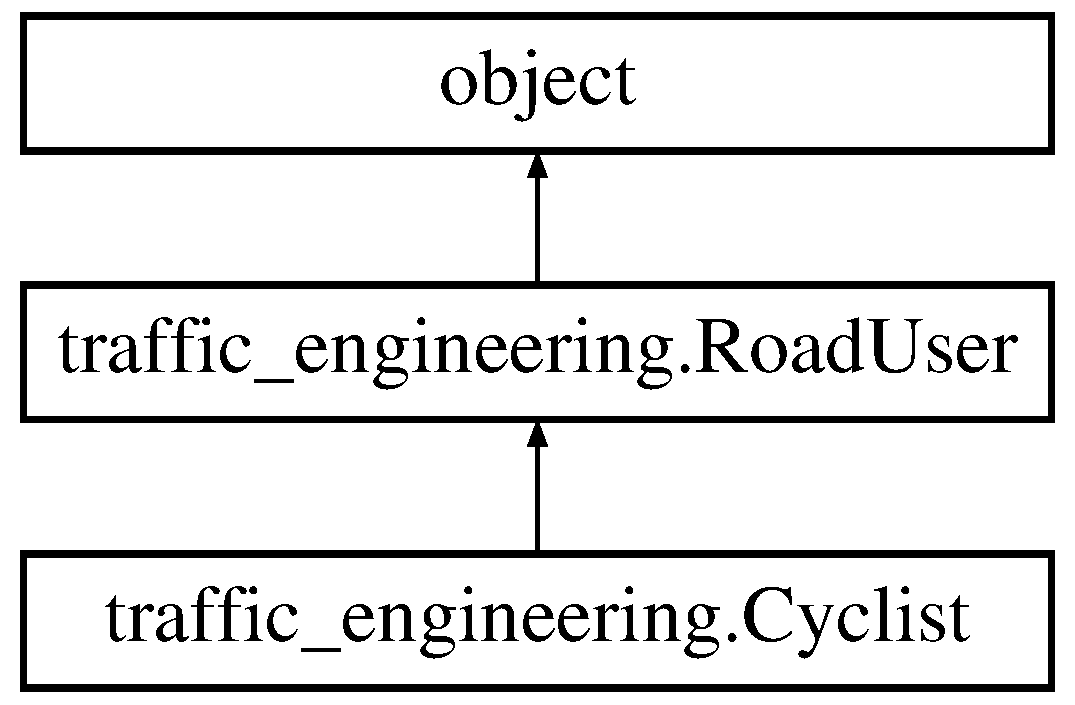
\includegraphics[height=3.000000cm]{classtraffic__engineering_1_1Cyclist}
\end{center}
\end{figure}
\subsubsection*{Public Member Functions}
\begin{DoxyCompactItemize}
\item 
def \hyperlink{classtraffic__engineering_1_1Cyclist_ae6e042e05b4f4e0630008c9e720f358d}{get\-Descriptor}
\end{DoxyCompactItemize}
\subsubsection*{Additional Inherited Members}


\subsubsection{Member Function Documentation}
\hypertarget{classtraffic__engineering_1_1Cyclist_ae6e042e05b4f4e0630008c9e720f358d}{\index{traffic\-\_\-engineering\-::\-Cyclist@{traffic\-\_\-engineering\-::\-Cyclist}!get\-Descriptor@{get\-Descriptor}}
\index{get\-Descriptor@{get\-Descriptor}!traffic_engineering::Cyclist@{traffic\-\_\-engineering\-::\-Cyclist}}
\paragraph[{get\-Descriptor}]{\setlength{\rightskip}{0pt plus 5cm}def traffic\-\_\-engineering.\-Cyclist.\-get\-Descriptor (
\begin{DoxyParamCaption}
\item[{}]{self}
\end{DoxyParamCaption}
)}}\label{classtraffic__engineering_1_1Cyclist_ae6e042e05b4f4e0630008c9e720f358d}


The documentation for this class was generated from the following file\-:\begin{DoxyCompactItemize}
\item 
python/\hyperlink{traffic__engineering_8py}{traffic\-\_\-engineering.\-py}\end{DoxyCompactItemize}

\hypertarget{classutils_1_1DiscreteDistributionSample}{\subsection{utils.\-Discrete\-Distribution\-Sample Class Reference}
\label{classutils_1_1DiscreteDistributionSample}\index{utils.\-Discrete\-Distribution\-Sample@{utils.\-Discrete\-Distribution\-Sample}}
}
Inheritance diagram for utils.\-Discrete\-Distribution\-Sample\-:\begin{figure}[H]
\begin{center}
\leavevmode
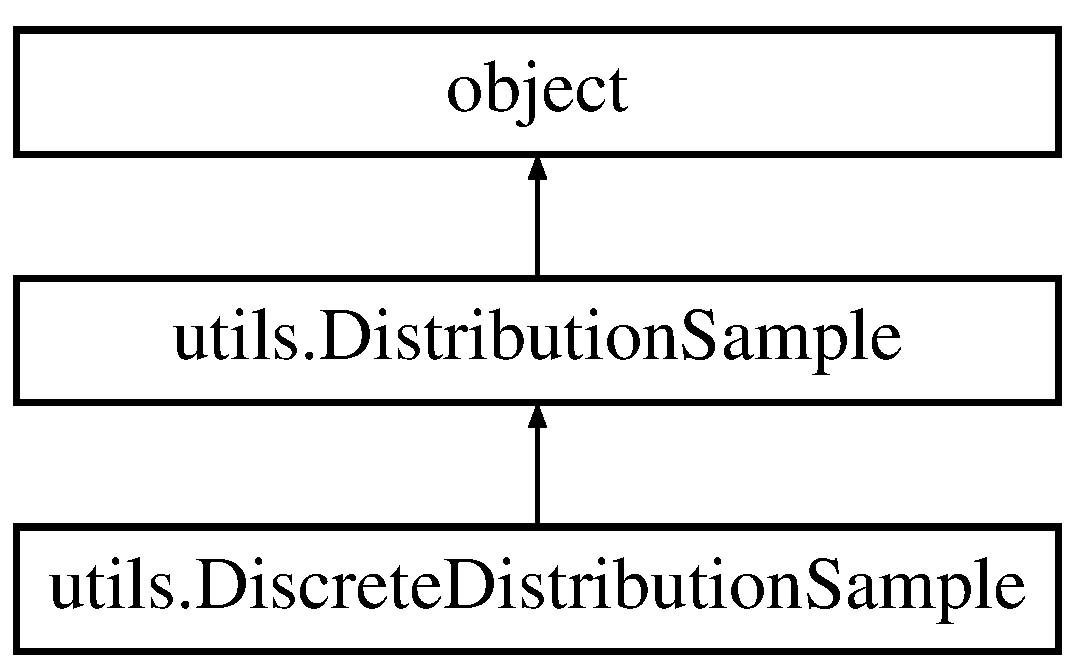
\includegraphics[height=3.000000cm]{classutils_1_1DiscreteDistributionSample}
\end{center}
\end{figure}
\subsubsection*{Public Member Functions}
\begin{DoxyCompactItemize}
\item 
def \hyperlink{classutils_1_1DiscreteDistributionSample_ad887c224af2bbd35f9295e04de237172}{\-\_\-\-\_\-init\-\_\-\-\_\-}
\item 
def \hyperlink{classutils_1_1DiscreteDistributionSample_a1eb09ddb48ca9c6d903fed7a0d1a5c18}{mean}
\item 
def \hyperlink{classutils_1_1DiscreteDistributionSample_a76e0b23eb39ea2c693ad09e1f80386ca}{var}
\item 
def \hyperlink{classutils_1_1DiscreteDistributionSample_a321a374395e5f4e56710a4a68d3b68a9}{reference\-Counts}
\end{DoxyCompactItemize}
\subsubsection*{Public Attributes}
\begin{DoxyCompactItemize}
\item 
\hyperlink{classutils_1_1DiscreteDistributionSample_afa78351d9f101acb84d2d2ad6bf71923}{categories}
\item 
\hyperlink{classutils_1_1DiscreteDistributionSample_a3521f264cfd39576b109fed45c45b5de}{counts}
\end{DoxyCompactItemize}


\subsubsection{Detailed Description}
\begin{DoxyVerb}Class to represent a sample of a distribution for a discrete random variable\end{DoxyVerb}
 

\subsubsection{Constructor \& Destructor Documentation}
\hypertarget{classutils_1_1DiscreteDistributionSample_ad887c224af2bbd35f9295e04de237172}{\index{utils\-::\-Discrete\-Distribution\-Sample@{utils\-::\-Discrete\-Distribution\-Sample}!\-\_\-\-\_\-init\-\_\-\-\_\-@{\-\_\-\-\_\-init\-\_\-\-\_\-}}
\index{\-\_\-\-\_\-init\-\_\-\-\_\-@{\-\_\-\-\_\-init\-\_\-\-\_\-}!utils::DiscreteDistributionSample@{utils\-::\-Discrete\-Distribution\-Sample}}
\paragraph[{\-\_\-\-\_\-init\-\_\-\-\_\-}]{\setlength{\rightskip}{0pt plus 5cm}def utils.\-Discrete\-Distribution\-Sample.\-\_\-\-\_\-init\-\_\-\-\_\- (
\begin{DoxyParamCaption}
\item[{}]{self, }
\item[{}]{categories, }
\item[{}]{counts}
\end{DoxyParamCaption}
)}}\label{classutils_1_1DiscreteDistributionSample_ad887c224af2bbd35f9295e04de237172}


\subsubsection{Member Function Documentation}
\hypertarget{classutils_1_1DiscreteDistributionSample_a1eb09ddb48ca9c6d903fed7a0d1a5c18}{\index{utils\-::\-Discrete\-Distribution\-Sample@{utils\-::\-Discrete\-Distribution\-Sample}!mean@{mean}}
\index{mean@{mean}!utils::DiscreteDistributionSample@{utils\-::\-Discrete\-Distribution\-Sample}}
\paragraph[{mean}]{\setlength{\rightskip}{0pt plus 5cm}def utils.\-Discrete\-Distribution\-Sample.\-mean (
\begin{DoxyParamCaption}
\item[{}]{self}
\end{DoxyParamCaption}
)}}\label{classutils_1_1DiscreteDistributionSample_a1eb09ddb48ca9c6d903fed7a0d1a5c18}


References events.\-Interaction.\-categories, utils.\-Discrete\-Distribution\-Sample.\-categories, utils.\-Discrete\-Distribution\-Sample.\-counts, and utils.\-Distribution\-Sample.\-n\-Samples().

\hypertarget{classutils_1_1DiscreteDistributionSample_a321a374395e5f4e56710a4a68d3b68a9}{\index{utils\-::\-Discrete\-Distribution\-Sample@{utils\-::\-Discrete\-Distribution\-Sample}!reference\-Counts@{reference\-Counts}}
\index{reference\-Counts@{reference\-Counts}!utils::DiscreteDistributionSample@{utils\-::\-Discrete\-Distribution\-Sample}}
\paragraph[{reference\-Counts}]{\setlength{\rightskip}{0pt plus 5cm}def utils.\-Discrete\-Distribution\-Sample.\-reference\-Counts (
\begin{DoxyParamCaption}
\item[{}]{self, }
\item[{}]{probability}
\end{DoxyParamCaption}
)}}\label{classutils_1_1DiscreteDistributionSample_a321a374395e5f4e56710a4a68d3b68a9}
\begin{DoxyVerb}probability is a function that returns the probability of the random variable for the category values\end{DoxyVerb}
 

References events.\-Interaction.\-categories, utils.\-Discrete\-Distribution\-Sample.\-categories, and utils.\-Distribution\-Sample.\-n\-Samples().

\hypertarget{classutils_1_1DiscreteDistributionSample_a76e0b23eb39ea2c693ad09e1f80386ca}{\index{utils\-::\-Discrete\-Distribution\-Sample@{utils\-::\-Discrete\-Distribution\-Sample}!var@{var}}
\index{var@{var}!utils::DiscreteDistributionSample@{utils\-::\-Discrete\-Distribution\-Sample}}
\paragraph[{var}]{\setlength{\rightskip}{0pt plus 5cm}def utils.\-Discrete\-Distribution\-Sample.\-var (
\begin{DoxyParamCaption}
\item[{}]{self, }
\item[{}]{mean = {\ttfamily None}}
\end{DoxyParamCaption}
)}}\label{classutils_1_1DiscreteDistributionSample_a76e0b23eb39ea2c693ad09e1f80386ca}


References events.\-Interaction.\-categories, utils.\-Discrete\-Distribution\-Sample.\-categories, utils.\-Discrete\-Distribution\-Sample.\-counts, utils.\-Discrete\-Distribution\-Sample.\-mean(), and utils.\-Distribution\-Sample.\-n\-Samples().



\subsubsection{Member Data Documentation}
\hypertarget{classutils_1_1DiscreteDistributionSample_afa78351d9f101acb84d2d2ad6bf71923}{\index{utils\-::\-Discrete\-Distribution\-Sample@{utils\-::\-Discrete\-Distribution\-Sample}!categories@{categories}}
\index{categories@{categories}!utils::DiscreteDistributionSample@{utils\-::\-Discrete\-Distribution\-Sample}}
\paragraph[{categories}]{\setlength{\rightskip}{0pt plus 5cm}utils.\-Discrete\-Distribution\-Sample.\-categories}}\label{classutils_1_1DiscreteDistributionSample_afa78351d9f101acb84d2d2ad6bf71923}
\hypertarget{classutils_1_1DiscreteDistributionSample_a3521f264cfd39576b109fed45c45b5de}{\index{utils\-::\-Discrete\-Distribution\-Sample@{utils\-::\-Discrete\-Distribution\-Sample}!counts@{counts}}
\index{counts@{counts}!utils::DiscreteDistributionSample@{utils\-::\-Discrete\-Distribution\-Sample}}
\paragraph[{counts}]{\setlength{\rightskip}{0pt plus 5cm}utils.\-Discrete\-Distribution\-Sample.\-counts}}\label{classutils_1_1DiscreteDistributionSample_a3521f264cfd39576b109fed45c45b5de}


The documentation for this class was generated from the following file\-:\begin{DoxyCompactItemize}
\item 
python/\hyperlink{utils_8py}{utils.\-py}\end{DoxyCompactItemize}

\hypertarget{classutils_1_1DistributionSample}{\subsection{utils.\-Distribution\-Sample Class Reference}
\label{classutils_1_1DistributionSample}\index{utils.\-Distribution\-Sample@{utils.\-Distribution\-Sample}}
}
Inheritance diagram for utils.\-Distribution\-Sample\-:\begin{figure}[H]
\begin{center}
\leavevmode
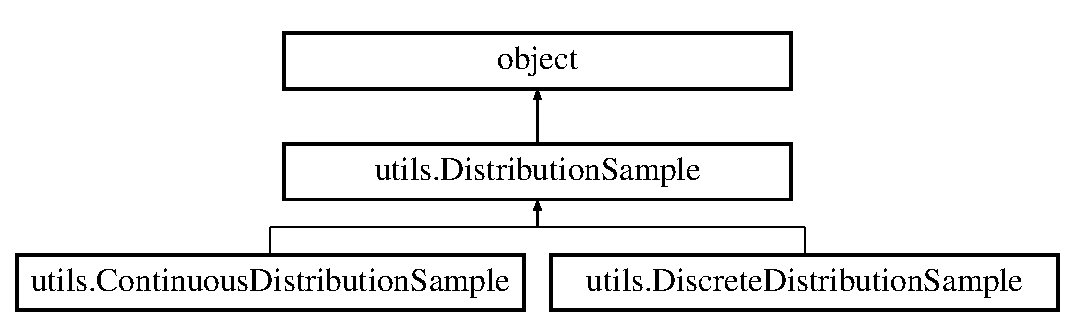
\includegraphics[height=3.000000cm]{classutils_1_1DistributionSample}
\end{center}
\end{figure}
\subsubsection*{Public Member Functions}
\begin{DoxyCompactItemize}
\item 
def \hyperlink{classutils_1_1DistributionSample_aeac9659673adb41dc19a01883c38246a}{n\-Samples}
\end{DoxyCompactItemize}


\subsubsection{Member Function Documentation}
\hypertarget{classutils_1_1DistributionSample_aeac9659673adb41dc19a01883c38246a}{\index{utils\-::\-Distribution\-Sample@{utils\-::\-Distribution\-Sample}!n\-Samples@{n\-Samples}}
\index{n\-Samples@{n\-Samples}!utils::DistributionSample@{utils\-::\-Distribution\-Sample}}
\paragraph[{n\-Samples}]{\setlength{\rightskip}{0pt plus 5cm}def utils.\-Distribution\-Sample.\-n\-Samples (
\begin{DoxyParamCaption}
\item[{}]{self}
\end{DoxyParamCaption}
)}}\label{classutils_1_1DistributionSample_aeac9659673adb41dc19a01883c38246a}


References utils.\-Discrete\-Distribution\-Sample.\-counts, and utils.\-Continuous\-Distribution\-Sample.\-counts.



The documentation for this class was generated from the following file\-:\begin{DoxyCompactItemize}
\item 
python/\hyperlink{utils_8py}{utils.\-py}\end{DoxyCompactItemize}

\hypertarget{structCatch_1_1Matchers_1_1Impl_1_1StdString_1_1EndsWith}{\subsection{Catch\-:\-:Matchers\-:\-:Impl\-:\-:Std\-String\-:\-:Ends\-With Struct Reference}
\label{structCatch_1_1Matchers_1_1Impl_1_1StdString_1_1EndsWith}\index{Catch\-::\-Matchers\-::\-Impl\-::\-Std\-String\-::\-Ends\-With@{Catch\-::\-Matchers\-::\-Impl\-::\-Std\-String\-::\-Ends\-With}}
}


{\ttfamily \#include $<$catch.\-hpp$>$}

\subsubsection*{Public Member Functions}
\begin{DoxyCompactItemize}
\item 
\hyperlink{structCatch_1_1Matchers_1_1Impl_1_1StdString_1_1EndsWith_ae8b4302029094a6486656b2d800e5e1f}{Ends\-With} (const std\-::string \&substr)
\item 
bool \hyperlink{structCatch_1_1Matchers_1_1Impl_1_1StdString_1_1EndsWith_a8baf52ce3d1693940244f496c64c119d}{operator()} (const std\-::string \&str) const 
\end{DoxyCompactItemize}
\subsubsection*{Public Attributes}
\begin{DoxyCompactItemize}
\item 
std\-::string \hyperlink{structCatch_1_1Matchers_1_1Impl_1_1StdString_1_1EndsWith_a5abf70e94ea7893b7bd1e7b33880ba7b}{m\-\_\-substr}
\end{DoxyCompactItemize}
\subsubsection*{Friends}
\begin{DoxyCompactItemize}
\item 
std\-::ostream \& \hyperlink{structCatch_1_1Matchers_1_1Impl_1_1StdString_1_1EndsWith_a3389586caac8a112f2413ecc3d155131}{operator$<$$<$} (std\-::ostream \&os, const \hyperlink{structCatch_1_1Matchers_1_1Impl_1_1StdString_1_1EndsWith}{Ends\-With} \&matcher)
\end{DoxyCompactItemize}


\subsubsection{Constructor \& Destructor Documentation}
\hypertarget{structCatch_1_1Matchers_1_1Impl_1_1StdString_1_1EndsWith_ae8b4302029094a6486656b2d800e5e1f}{\index{Catch\-::\-Matchers\-::\-Impl\-::\-Std\-String\-::\-Ends\-With@{Catch\-::\-Matchers\-::\-Impl\-::\-Std\-String\-::\-Ends\-With}!Ends\-With@{Ends\-With}}
\index{Ends\-With@{Ends\-With}!Catch::Matchers::Impl::StdString::EndsWith@{Catch\-::\-Matchers\-::\-Impl\-::\-Std\-String\-::\-Ends\-With}}
\paragraph[{Ends\-With}]{\setlength{\rightskip}{0pt plus 5cm}Catch\-::\-Matchers\-::\-Impl\-::\-Std\-String\-::\-Ends\-With\-::\-Ends\-With (
\begin{DoxyParamCaption}
\item[{const std\-::string \&}]{substr}
\end{DoxyParamCaption}
)\hspace{0.3cm}{\ttfamily [inline]}}}\label{structCatch_1_1Matchers_1_1Impl_1_1StdString_1_1EndsWith_ae8b4302029094a6486656b2d800e5e1f}


\subsubsection{Member Function Documentation}
\hypertarget{structCatch_1_1Matchers_1_1Impl_1_1StdString_1_1EndsWith_a8baf52ce3d1693940244f496c64c119d}{\index{Catch\-::\-Matchers\-::\-Impl\-::\-Std\-String\-::\-Ends\-With@{Catch\-::\-Matchers\-::\-Impl\-::\-Std\-String\-::\-Ends\-With}!operator()@{operator()}}
\index{operator()@{operator()}!Catch::Matchers::Impl::StdString::EndsWith@{Catch\-::\-Matchers\-::\-Impl\-::\-Std\-String\-::\-Ends\-With}}
\paragraph[{operator()}]{\setlength{\rightskip}{0pt plus 5cm}bool Catch\-::\-Matchers\-::\-Impl\-::\-Std\-String\-::\-Ends\-With\-::operator() (
\begin{DoxyParamCaption}
\item[{const std\-::string \&}]{str}
\end{DoxyParamCaption}
) const\hspace{0.3cm}{\ttfamily [inline]}}}\label{structCatch_1_1Matchers_1_1Impl_1_1StdString_1_1EndsWith_a8baf52ce3d1693940244f496c64c119d}


References m\-\_\-substr.



\subsubsection{Friends And Related Function Documentation}
\hypertarget{structCatch_1_1Matchers_1_1Impl_1_1StdString_1_1EndsWith_a3389586caac8a112f2413ecc3d155131}{\index{Catch\-::\-Matchers\-::\-Impl\-::\-Std\-String\-::\-Ends\-With@{Catch\-::\-Matchers\-::\-Impl\-::\-Std\-String\-::\-Ends\-With}!operator$<$$<$@{operator$<$$<$}}
\index{operator$<$$<$@{operator$<$$<$}!Catch::Matchers::Impl::StdString::EndsWith@{Catch\-::\-Matchers\-::\-Impl\-::\-Std\-String\-::\-Ends\-With}}
\paragraph[{operator$<$$<$}]{\setlength{\rightskip}{0pt plus 5cm}std\-::ostream\& operator$<$$<$ (
\begin{DoxyParamCaption}
\item[{std\-::ostream \&}]{os, }
\item[{const {\bf Ends\-With} \&}]{matcher}
\end{DoxyParamCaption}
)\hspace{0.3cm}{\ttfamily [friend]}}}\label{structCatch_1_1Matchers_1_1Impl_1_1StdString_1_1EndsWith_a3389586caac8a112f2413ecc3d155131}


\subsubsection{Member Data Documentation}
\hypertarget{structCatch_1_1Matchers_1_1Impl_1_1StdString_1_1EndsWith_a5abf70e94ea7893b7bd1e7b33880ba7b}{\index{Catch\-::\-Matchers\-::\-Impl\-::\-Std\-String\-::\-Ends\-With@{Catch\-::\-Matchers\-::\-Impl\-::\-Std\-String\-::\-Ends\-With}!m\-\_\-substr@{m\-\_\-substr}}
\index{m\-\_\-substr@{m\-\_\-substr}!Catch::Matchers::Impl::StdString::EndsWith@{Catch\-::\-Matchers\-::\-Impl\-::\-Std\-String\-::\-Ends\-With}}
\paragraph[{m\-\_\-substr}]{\setlength{\rightskip}{0pt plus 5cm}std\-::string Catch\-::\-Matchers\-::\-Impl\-::\-Std\-String\-::\-Ends\-With\-::m\-\_\-substr}}\label{structCatch_1_1Matchers_1_1Impl_1_1StdString_1_1EndsWith_a5abf70e94ea7893b7bd1e7b33880ba7b}


The documentation for this struct was generated from the following file\-:\begin{DoxyCompactItemize}
\item 
include/\hyperlink{catch_8hpp}{catch.\-hpp}\end{DoxyCompactItemize}

\hypertarget{classmetadata_1_1EnvironementalFactors}{\subsection{metadata.\-Environemental\-Factors Class Reference}
\label{classmetadata_1_1EnvironementalFactors}\index{metadata.\-Environemental\-Factors@{metadata.\-Environemental\-Factors}}
}
Inheritance diagram for metadata.\-Environemental\-Factors\-:\begin{figure}[H]
\begin{center}
\leavevmode
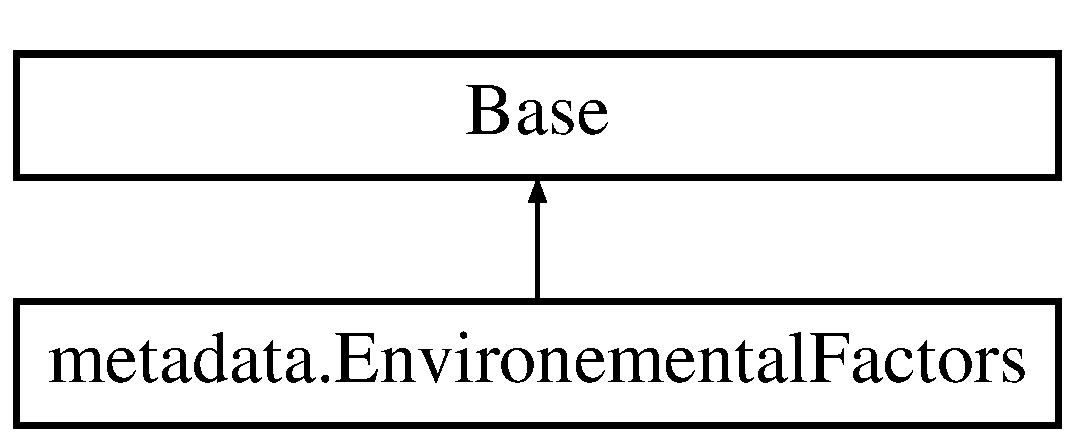
\includegraphics[height=2.000000cm]{classmetadata_1_1EnvironementalFactors}
\end{center}
\end{figure}
\subsubsection*{Public Member Functions}
\begin{DoxyCompactItemize}
\item 
def \hyperlink{classmetadata_1_1EnvironementalFactors_af3c8720509a7bc9b2a610870d6aa7393}{\-\_\-\-\_\-init\-\_\-\-\_\-}
\end{DoxyCompactItemize}
\subsubsection*{Public Attributes}
\begin{DoxyCompactItemize}
\item 
\hyperlink{classmetadata_1_1EnvironementalFactors_a06cee8a6fd4c3ef2d4e9efd6e3361693}{start\-Time}
\item 
\hyperlink{classmetadata_1_1EnvironementalFactors_a12176448537de9e783ce7338fa601afb}{end\-Time}
\item 
\hyperlink{classmetadata_1_1EnvironementalFactors_a8a36643a488632dba000e1a4b62c7c63}{description}
\item 
\hyperlink{classmetadata_1_1EnvironementalFactors_a131e9008b6c7ea2a1db5bc8711035a64}{site}
\end{DoxyCompactItemize}
\subsubsection*{Static Public Attributes}
\begin{DoxyCompactItemize}
\item 
tuple \hyperlink{classmetadata_1_1EnvironementalFactors_ae098f6dc54e0df53a8e40b63ad8f2950}{idx} = Column(Integer, primary\-\_\-key=True)
\item 
tuple \hyperlink{classmetadata_1_1EnvironementalFactors_afecc3211391a18b1750051da30ea0bfc}{start\-Time} = Column(Date\-Time)
\item 
tuple \hyperlink{classmetadata_1_1EnvironementalFactors_a68f7a51d43489a9eaeb8d103860f9158}{end\-Time} = Column(Date\-Time)
\item 
tuple \hyperlink{classmetadata_1_1EnvironementalFactors_a8d362ee1e898cf877c83edbe9f0c971e}{description} = Column(String)
\item 
tuple \hyperlink{classmetadata_1_1EnvironementalFactors_ad244fb9dc07336c2284a8d74c3ec10a7}{site\-Idx} = Column(Integer, Foreign\-Key('sites.\-idx'))
\item 
tuple \hyperlink{classmetadata_1_1EnvironementalFactors_a2d1bb47f71311626cc0023b26530edbb}{site} = relationship(\char`\"{}Site\char`\"{}, backref=backref('environmental\-\_\-factors', order\-\_\-by = \hyperlink{classmetadata_1_1EnvironementalFactors_ae098f6dc54e0df53a8e40b63ad8f2950}{idx}))
\end{DoxyCompactItemize}


\subsubsection{Detailed Description}
\begin{DoxyVerb}Represents any environmental factors that may affect the results, in particular
* changing weather conditions
* changing road configuration, geometry, signalization, etc.
ex: sunny, rainy, before counter-measure, after counter-measure\end{DoxyVerb}
 

\subsubsection{Constructor \& Destructor Documentation}
\hypertarget{classmetadata_1_1EnvironementalFactors_af3c8720509a7bc9b2a610870d6aa7393}{\index{metadata\-::\-Environemental\-Factors@{metadata\-::\-Environemental\-Factors}!\-\_\-\-\_\-init\-\_\-\-\_\-@{\-\_\-\-\_\-init\-\_\-\-\_\-}}
\index{\-\_\-\-\_\-init\-\_\-\-\_\-@{\-\_\-\-\_\-init\-\_\-\-\_\-}!metadata::EnvironementalFactors@{metadata\-::\-Environemental\-Factors}}
\paragraph[{\-\_\-\-\_\-init\-\_\-\-\_\-}]{\setlength{\rightskip}{0pt plus 5cm}def metadata.\-Environemental\-Factors.\-\_\-\-\_\-init\-\_\-\-\_\- (
\begin{DoxyParamCaption}
\item[{}]{self, }
\item[{}]{start\-Time, }
\item[{}]{end\-Time, }
\item[{}]{description, }
\item[{}]{site}
\end{DoxyParamCaption}
)}}\label{classmetadata_1_1EnvironementalFactors_af3c8720509a7bc9b2a610870d6aa7393}


\subsubsection{Member Data Documentation}
\hypertarget{classmetadata_1_1EnvironementalFactors_a8d362ee1e898cf877c83edbe9f0c971e}{\index{metadata\-::\-Environemental\-Factors@{metadata\-::\-Environemental\-Factors}!description@{description}}
\index{description@{description}!metadata::EnvironementalFactors@{metadata\-::\-Environemental\-Factors}}
\paragraph[{description}]{\setlength{\rightskip}{0pt plus 5cm}tuple metadata.\-Environemental\-Factors.\-description = Column(String)\hspace{0.3cm}{\ttfamily [static]}}}\label{classmetadata_1_1EnvironementalFactors_a8d362ee1e898cf877c83edbe9f0c971e}
\hypertarget{classmetadata_1_1EnvironementalFactors_a8a36643a488632dba000e1a4b62c7c63}{\index{metadata\-::\-Environemental\-Factors@{metadata\-::\-Environemental\-Factors}!description@{description}}
\index{description@{description}!metadata::EnvironementalFactors@{metadata\-::\-Environemental\-Factors}}
\paragraph[{description}]{\setlength{\rightskip}{0pt plus 5cm}metadata.\-Environemental\-Factors.\-description}}\label{classmetadata_1_1EnvironementalFactors_a8a36643a488632dba000e1a4b62c7c63}
\hypertarget{classmetadata_1_1EnvironementalFactors_a68f7a51d43489a9eaeb8d103860f9158}{\index{metadata\-::\-Environemental\-Factors@{metadata\-::\-Environemental\-Factors}!end\-Time@{end\-Time}}
\index{end\-Time@{end\-Time}!metadata::EnvironementalFactors@{metadata\-::\-Environemental\-Factors}}
\paragraph[{end\-Time}]{\setlength{\rightskip}{0pt plus 5cm}tuple metadata.\-Environemental\-Factors.\-end\-Time = Column(Date\-Time)\hspace{0.3cm}{\ttfamily [static]}}}\label{classmetadata_1_1EnvironementalFactors_a68f7a51d43489a9eaeb8d103860f9158}
\hypertarget{classmetadata_1_1EnvironementalFactors_a12176448537de9e783ce7338fa601afb}{\index{metadata\-::\-Environemental\-Factors@{metadata\-::\-Environemental\-Factors}!end\-Time@{end\-Time}}
\index{end\-Time@{end\-Time}!metadata::EnvironementalFactors@{metadata\-::\-Environemental\-Factors}}
\paragraph[{end\-Time}]{\setlength{\rightskip}{0pt plus 5cm}metadata.\-Environemental\-Factors.\-end\-Time}}\label{classmetadata_1_1EnvironementalFactors_a12176448537de9e783ce7338fa601afb}
\hypertarget{classmetadata_1_1EnvironementalFactors_ae098f6dc54e0df53a8e40b63ad8f2950}{\index{metadata\-::\-Environemental\-Factors@{metadata\-::\-Environemental\-Factors}!idx@{idx}}
\index{idx@{idx}!metadata::EnvironementalFactors@{metadata\-::\-Environemental\-Factors}}
\paragraph[{idx}]{\setlength{\rightskip}{0pt plus 5cm}tuple metadata.\-Environemental\-Factors.\-idx = Column(Integer, primary\-\_\-key=True)\hspace{0.3cm}{\ttfamily [static]}}}\label{classmetadata_1_1EnvironementalFactors_ae098f6dc54e0df53a8e40b63ad8f2950}
\hypertarget{classmetadata_1_1EnvironementalFactors_a2d1bb47f71311626cc0023b26530edbb}{\index{metadata\-::\-Environemental\-Factors@{metadata\-::\-Environemental\-Factors}!site@{site}}
\index{site@{site}!metadata::EnvironementalFactors@{metadata\-::\-Environemental\-Factors}}
\paragraph[{site}]{\setlength{\rightskip}{0pt plus 5cm}tuple metadata.\-Environemental\-Factors.\-site = relationship(\char`\"{}Site\char`\"{}, backref=backref('environmental\-\_\-factors', order\-\_\-by = {\bf idx}))\hspace{0.3cm}{\ttfamily [static]}}}\label{classmetadata_1_1EnvironementalFactors_a2d1bb47f71311626cc0023b26530edbb}
\hypertarget{classmetadata_1_1EnvironementalFactors_a131e9008b6c7ea2a1db5bc8711035a64}{\index{metadata\-::\-Environemental\-Factors@{metadata\-::\-Environemental\-Factors}!site@{site}}
\index{site@{site}!metadata::EnvironementalFactors@{metadata\-::\-Environemental\-Factors}}
\paragraph[{site}]{\setlength{\rightskip}{0pt plus 5cm}metadata.\-Environemental\-Factors.\-site}}\label{classmetadata_1_1EnvironementalFactors_a131e9008b6c7ea2a1db5bc8711035a64}
\hypertarget{classmetadata_1_1EnvironementalFactors_ad244fb9dc07336c2284a8d74c3ec10a7}{\index{metadata\-::\-Environemental\-Factors@{metadata\-::\-Environemental\-Factors}!site\-Idx@{site\-Idx}}
\index{site\-Idx@{site\-Idx}!metadata::EnvironementalFactors@{metadata\-::\-Environemental\-Factors}}
\paragraph[{site\-Idx}]{\setlength{\rightskip}{0pt plus 5cm}tuple metadata.\-Environemental\-Factors.\-site\-Idx = Column(Integer, Foreign\-Key('sites.\-idx'))\hspace{0.3cm}{\ttfamily [static]}}}\label{classmetadata_1_1EnvironementalFactors_ad244fb9dc07336c2284a8d74c3ec10a7}
\hypertarget{classmetadata_1_1EnvironementalFactors_afecc3211391a18b1750051da30ea0bfc}{\index{metadata\-::\-Environemental\-Factors@{metadata\-::\-Environemental\-Factors}!start\-Time@{start\-Time}}
\index{start\-Time@{start\-Time}!metadata::EnvironementalFactors@{metadata\-::\-Environemental\-Factors}}
\paragraph[{start\-Time}]{\setlength{\rightskip}{0pt plus 5cm}tuple metadata.\-Environemental\-Factors.\-start\-Time = Column(Date\-Time)\hspace{0.3cm}{\ttfamily [static]}}}\label{classmetadata_1_1EnvironementalFactors_afecc3211391a18b1750051da30ea0bfc}
\hypertarget{classmetadata_1_1EnvironementalFactors_a06cee8a6fd4c3ef2d4e9efd6e3361693}{\index{metadata\-::\-Environemental\-Factors@{metadata\-::\-Environemental\-Factors}!start\-Time@{start\-Time}}
\index{start\-Time@{start\-Time}!metadata::EnvironementalFactors@{metadata\-::\-Environemental\-Factors}}
\paragraph[{start\-Time}]{\setlength{\rightskip}{0pt plus 5cm}metadata.\-Environemental\-Factors.\-start\-Time}}\label{classmetadata_1_1EnvironementalFactors_a06cee8a6fd4c3ef2d4e9efd6e3361693}


The documentation for this class was generated from the following file\-:\begin{DoxyCompactItemize}
\item 
python/\hyperlink{metadata_8py}{metadata.\-py}\end{DoxyCompactItemize}

\hypertarget{structCatch_1_1Matchers_1_1Impl_1_1StdString_1_1Equals}{\subsection{Catch\-:\-:Matchers\-:\-:Impl\-:\-:Std\-String\-:\-:Equals Struct Reference}
\label{structCatch_1_1Matchers_1_1Impl_1_1StdString_1_1Equals}\index{Catch\-::\-Matchers\-::\-Impl\-::\-Std\-String\-::\-Equals@{Catch\-::\-Matchers\-::\-Impl\-::\-Std\-String\-::\-Equals}}
}


{\ttfamily \#include $<$catch.\-hpp$>$}

\subsubsection*{Public Member Functions}
\begin{DoxyCompactItemize}
\item 
\hyperlink{structCatch_1_1Matchers_1_1Impl_1_1StdString_1_1Equals_a11a973d939bcf2ee056157f43bdfb536}{Equals} (const std\-::string \&str)
\item 
bool \hyperlink{structCatch_1_1Matchers_1_1Impl_1_1StdString_1_1Equals_aa6c1e3ad1e27d3569cfb38d89e7e1a2c}{operator()} (const std\-::string \&str) const 
\end{DoxyCompactItemize}
\subsubsection*{Public Attributes}
\begin{DoxyCompactItemize}
\item 
std\-::string \hyperlink{structCatch_1_1Matchers_1_1Impl_1_1StdString_1_1Equals_a41fc4413185f47d8b6d8da7a55078921}{m\-\_\-str}
\end{DoxyCompactItemize}
\subsubsection*{Friends}
\begin{DoxyCompactItemize}
\item 
std\-::ostream \& \hyperlink{structCatch_1_1Matchers_1_1Impl_1_1StdString_1_1Equals_a373e9d0e4cc18bd5ffa530140e035387}{operator$<$$<$} (std\-::ostream \&os, const \hyperlink{structCatch_1_1Matchers_1_1Impl_1_1StdString_1_1Equals}{Equals} \&matcher)
\end{DoxyCompactItemize}


\subsubsection{Constructor \& Destructor Documentation}
\hypertarget{structCatch_1_1Matchers_1_1Impl_1_1StdString_1_1Equals_a11a973d939bcf2ee056157f43bdfb536}{\index{Catch\-::\-Matchers\-::\-Impl\-::\-Std\-String\-::\-Equals@{Catch\-::\-Matchers\-::\-Impl\-::\-Std\-String\-::\-Equals}!Equals@{Equals}}
\index{Equals@{Equals}!Catch::Matchers::Impl::StdString::Equals@{Catch\-::\-Matchers\-::\-Impl\-::\-Std\-String\-::\-Equals}}
\paragraph[{Equals}]{\setlength{\rightskip}{0pt plus 5cm}Catch\-::\-Matchers\-::\-Impl\-::\-Std\-String\-::\-Equals\-::\-Equals (
\begin{DoxyParamCaption}
\item[{const std\-::string \&}]{str}
\end{DoxyParamCaption}
)\hspace{0.3cm}{\ttfamily [inline]}}}\label{structCatch_1_1Matchers_1_1Impl_1_1StdString_1_1Equals_a11a973d939bcf2ee056157f43bdfb536}


\subsubsection{Member Function Documentation}
\hypertarget{structCatch_1_1Matchers_1_1Impl_1_1StdString_1_1Equals_aa6c1e3ad1e27d3569cfb38d89e7e1a2c}{\index{Catch\-::\-Matchers\-::\-Impl\-::\-Std\-String\-::\-Equals@{Catch\-::\-Matchers\-::\-Impl\-::\-Std\-String\-::\-Equals}!operator()@{operator()}}
\index{operator()@{operator()}!Catch::Matchers::Impl::StdString::Equals@{Catch\-::\-Matchers\-::\-Impl\-::\-Std\-String\-::\-Equals}}
\paragraph[{operator()}]{\setlength{\rightskip}{0pt plus 5cm}bool Catch\-::\-Matchers\-::\-Impl\-::\-Std\-String\-::\-Equals\-::operator() (
\begin{DoxyParamCaption}
\item[{const std\-::string \&}]{str}
\end{DoxyParamCaption}
) const\hspace{0.3cm}{\ttfamily [inline]}}}\label{structCatch_1_1Matchers_1_1Impl_1_1StdString_1_1Equals_aa6c1e3ad1e27d3569cfb38d89e7e1a2c}


References m\-\_\-str.



\subsubsection{Friends And Related Function Documentation}
\hypertarget{structCatch_1_1Matchers_1_1Impl_1_1StdString_1_1Equals_a373e9d0e4cc18bd5ffa530140e035387}{\index{Catch\-::\-Matchers\-::\-Impl\-::\-Std\-String\-::\-Equals@{Catch\-::\-Matchers\-::\-Impl\-::\-Std\-String\-::\-Equals}!operator$<$$<$@{operator$<$$<$}}
\index{operator$<$$<$@{operator$<$$<$}!Catch::Matchers::Impl::StdString::Equals@{Catch\-::\-Matchers\-::\-Impl\-::\-Std\-String\-::\-Equals}}
\paragraph[{operator$<$$<$}]{\setlength{\rightskip}{0pt plus 5cm}std\-::ostream\& operator$<$$<$ (
\begin{DoxyParamCaption}
\item[{std\-::ostream \&}]{os, }
\item[{const {\bf Equals} \&}]{matcher}
\end{DoxyParamCaption}
)\hspace{0.3cm}{\ttfamily [friend]}}}\label{structCatch_1_1Matchers_1_1Impl_1_1StdString_1_1Equals_a373e9d0e4cc18bd5ffa530140e035387}


\subsubsection{Member Data Documentation}
\hypertarget{structCatch_1_1Matchers_1_1Impl_1_1StdString_1_1Equals_a41fc4413185f47d8b6d8da7a55078921}{\index{Catch\-::\-Matchers\-::\-Impl\-::\-Std\-String\-::\-Equals@{Catch\-::\-Matchers\-::\-Impl\-::\-Std\-String\-::\-Equals}!m\-\_\-str@{m\-\_\-str}}
\index{m\-\_\-str@{m\-\_\-str}!Catch::Matchers::Impl::StdString::Equals@{Catch\-::\-Matchers\-::\-Impl\-::\-Std\-String\-::\-Equals}}
\paragraph[{m\-\_\-str}]{\setlength{\rightskip}{0pt plus 5cm}std\-::string Catch\-::\-Matchers\-::\-Impl\-::\-Std\-String\-::\-Equals\-::m\-\_\-str}}\label{structCatch_1_1Matchers_1_1Impl_1_1StdString_1_1Equals_a41fc4413185f47d8b6d8da7a55078921}


The documentation for this struct was generated from the following file\-:\begin{DoxyCompactItemize}
\item 
include/\hyperlink{catch_8hpp}{catch.\-hpp}\end{DoxyCompactItemize}

\hypertarget{classCatch_1_1Internal_1_1Evaluator}{\subsection{Catch\-:\-:Internal\-:\-:Evaluator$<$ T1, T2, Op $>$ Class Template Reference}
\label{classCatch_1_1Internal_1_1Evaluator}\index{Catch\-::\-Internal\-::\-Evaluator$<$ T1, T2, Op $>$@{Catch\-::\-Internal\-::\-Evaluator$<$ T1, T2, Op $>$}}
}


{\ttfamily \#include $<$catch.\-hpp$>$}



The documentation for this class was generated from the following file\-:\begin{DoxyCompactItemize}
\item 
include/\hyperlink{catch_8hpp}{catch.\-hpp}\end{DoxyCompactItemize}

\hypertarget{structCatch_1_1Internal_1_1Evaluator_3_01T1_00_01T2_00_01IsEqualTo_01_4}{\subsection{Catch\-:\-:Internal\-:\-:Evaluator$<$ T1, T2, Is\-Equal\-To $>$ Struct Template Reference}
\label{structCatch_1_1Internal_1_1Evaluator_3_01T1_00_01T2_00_01IsEqualTo_01_4}\index{Catch\-::\-Internal\-::\-Evaluator$<$ T1, T2, Is\-Equal\-To $>$@{Catch\-::\-Internal\-::\-Evaluator$<$ T1, T2, Is\-Equal\-To $>$}}
}


{\ttfamily \#include $<$catch.\-hpp$>$}

\subsubsection*{Static Public Member Functions}
\begin{DoxyCompactItemize}
\item 
static bool \hyperlink{structCatch_1_1Internal_1_1Evaluator_3_01T1_00_01T2_00_01IsEqualTo_01_4_a431f1bd4594c031017e70c378761d8b4}{evaluate} (const T1 \&lhs, const T2 \&rhs)
\end{DoxyCompactItemize}


\subsubsection{Member Function Documentation}
\hypertarget{structCatch_1_1Internal_1_1Evaluator_3_01T1_00_01T2_00_01IsEqualTo_01_4_a431f1bd4594c031017e70c378761d8b4}{\index{Catch\-::\-Internal\-::\-Evaluator$<$ T1, T2, Is\-Equal\-To $>$@{Catch\-::\-Internal\-::\-Evaluator$<$ T1, T2, Is\-Equal\-To $>$}!evaluate@{evaluate}}
\index{evaluate@{evaluate}!Catch::Internal::Evaluator< T1, T2, IsEqualTo >@{Catch\-::\-Internal\-::\-Evaluator$<$ T1, T2, Is\-Equal\-To $>$}}
\paragraph[{evaluate}]{\setlength{\rightskip}{0pt plus 5cm}template$<$typename T1 , typename T2 $>$ static bool {\bf Catch\-::\-Internal\-::\-Evaluator}$<$ T1, T2, {\bf Is\-Equal\-To} $>$\-::evaluate (
\begin{DoxyParamCaption}
\item[{const T1 \&}]{lhs, }
\item[{const T2 \&}]{rhs}
\end{DoxyParamCaption}
)\hspace{0.3cm}{\ttfamily [inline]}, {\ttfamily [static]}}}\label{structCatch_1_1Internal_1_1Evaluator_3_01T1_00_01T2_00_01IsEqualTo_01_4_a431f1bd4594c031017e70c378761d8b4}


The documentation for this struct was generated from the following file\-:\begin{DoxyCompactItemize}
\item 
include/\hyperlink{catch_8hpp}{catch.\-hpp}\end{DoxyCompactItemize}

\hypertarget{structCatch_1_1Internal_1_1Evaluator_3_01T1_00_01T2_00_01IsGreaterThan_01_4}{\subsection{Catch\-:\-:Internal\-:\-:Evaluator$<$ T1, T2, Is\-Greater\-Than $>$ Struct Template Reference}
\label{structCatch_1_1Internal_1_1Evaluator_3_01T1_00_01T2_00_01IsGreaterThan_01_4}\index{Catch\-::\-Internal\-::\-Evaluator$<$ T1, T2, Is\-Greater\-Than $>$@{Catch\-::\-Internal\-::\-Evaluator$<$ T1, T2, Is\-Greater\-Than $>$}}
}


{\ttfamily \#include $<$catch.\-hpp$>$}

\subsubsection*{Static Public Member Functions}
\begin{DoxyCompactItemize}
\item 
static bool \hyperlink{structCatch_1_1Internal_1_1Evaluator_3_01T1_00_01T2_00_01IsGreaterThan_01_4_ac3ea1a985441ab97c362517e59a6317b}{evaluate} (const T1 \&lhs, const T2 \&rhs)
\end{DoxyCompactItemize}


\subsubsection{Member Function Documentation}
\hypertarget{structCatch_1_1Internal_1_1Evaluator_3_01T1_00_01T2_00_01IsGreaterThan_01_4_ac3ea1a985441ab97c362517e59a6317b}{\index{Catch\-::\-Internal\-::\-Evaluator$<$ T1, T2, Is\-Greater\-Than $>$@{Catch\-::\-Internal\-::\-Evaluator$<$ T1, T2, Is\-Greater\-Than $>$}!evaluate@{evaluate}}
\index{evaluate@{evaluate}!Catch::Internal::Evaluator< T1, T2, IsGreaterThan >@{Catch\-::\-Internal\-::\-Evaluator$<$ T1, T2, Is\-Greater\-Than $>$}}
\paragraph[{evaluate}]{\setlength{\rightskip}{0pt plus 5cm}template$<$typename T1 , typename T2 $>$ static bool {\bf Catch\-::\-Internal\-::\-Evaluator}$<$ T1, T2, {\bf Is\-Greater\-Than} $>$\-::evaluate (
\begin{DoxyParamCaption}
\item[{const T1 \&}]{lhs, }
\item[{const T2 \&}]{rhs}
\end{DoxyParamCaption}
)\hspace{0.3cm}{\ttfamily [inline]}, {\ttfamily [static]}}}\label{structCatch_1_1Internal_1_1Evaluator_3_01T1_00_01T2_00_01IsGreaterThan_01_4_ac3ea1a985441ab97c362517e59a6317b}


The documentation for this struct was generated from the following file\-:\begin{DoxyCompactItemize}
\item 
include/\hyperlink{catch_8hpp}{catch.\-hpp}\end{DoxyCompactItemize}

\hypertarget{structCatch_1_1Internal_1_1Evaluator_3_01T1_00_01T2_00_01IsGreaterThanOrEqualTo_01_4}{\subsection{Catch\-:\-:Internal\-:\-:Evaluator$<$ T1, T2, Is\-Greater\-Than\-Or\-Equal\-To $>$ Struct Template Reference}
\label{structCatch_1_1Internal_1_1Evaluator_3_01T1_00_01T2_00_01IsGreaterThanOrEqualTo_01_4}\index{Catch\-::\-Internal\-::\-Evaluator$<$ T1, T2, Is\-Greater\-Than\-Or\-Equal\-To $>$@{Catch\-::\-Internal\-::\-Evaluator$<$ T1, T2, Is\-Greater\-Than\-Or\-Equal\-To $>$}}
}


{\ttfamily \#include $<$catch.\-hpp$>$}

\subsubsection*{Static Public Member Functions}
\begin{DoxyCompactItemize}
\item 
static bool \hyperlink{structCatch_1_1Internal_1_1Evaluator_3_01T1_00_01T2_00_01IsGreaterThanOrEqualTo_01_4_a9eedb75e0642ab8e6be995641cbc40de}{evaluate} (const T1 \&lhs, const T2 \&rhs)
\end{DoxyCompactItemize}


\subsubsection{Member Function Documentation}
\hypertarget{structCatch_1_1Internal_1_1Evaluator_3_01T1_00_01T2_00_01IsGreaterThanOrEqualTo_01_4_a9eedb75e0642ab8e6be995641cbc40de}{\index{Catch\-::\-Internal\-::\-Evaluator$<$ T1, T2, Is\-Greater\-Than\-Or\-Equal\-To $>$@{Catch\-::\-Internal\-::\-Evaluator$<$ T1, T2, Is\-Greater\-Than\-Or\-Equal\-To $>$}!evaluate@{evaluate}}
\index{evaluate@{evaluate}!Catch::Internal::Evaluator< T1, T2, IsGreaterThanOrEqualTo >@{Catch\-::\-Internal\-::\-Evaluator$<$ T1, T2, Is\-Greater\-Than\-Or\-Equal\-To $>$}}
\paragraph[{evaluate}]{\setlength{\rightskip}{0pt plus 5cm}template$<$typename T1 , typename T2 $>$ static bool {\bf Catch\-::\-Internal\-::\-Evaluator}$<$ T1, T2, {\bf Is\-Greater\-Than\-Or\-Equal\-To} $>$\-::evaluate (
\begin{DoxyParamCaption}
\item[{const T1 \&}]{lhs, }
\item[{const T2 \&}]{rhs}
\end{DoxyParamCaption}
)\hspace{0.3cm}{\ttfamily [inline]}, {\ttfamily [static]}}}\label{structCatch_1_1Internal_1_1Evaluator_3_01T1_00_01T2_00_01IsGreaterThanOrEqualTo_01_4_a9eedb75e0642ab8e6be995641cbc40de}


The documentation for this struct was generated from the following file\-:\begin{DoxyCompactItemize}
\item 
include/\hyperlink{catch_8hpp}{catch.\-hpp}\end{DoxyCompactItemize}

\hypertarget{structCatch_1_1Internal_1_1Evaluator_3_01T1_00_01T2_00_01IsLessThan_01_4}{\subsection{Catch\-:\-:Internal\-:\-:Evaluator$<$ T1, T2, Is\-Less\-Than $>$ Struct Template Reference}
\label{structCatch_1_1Internal_1_1Evaluator_3_01T1_00_01T2_00_01IsLessThan_01_4}\index{Catch\-::\-Internal\-::\-Evaluator$<$ T1, T2, Is\-Less\-Than $>$@{Catch\-::\-Internal\-::\-Evaluator$<$ T1, T2, Is\-Less\-Than $>$}}
}


{\ttfamily \#include $<$catch.\-hpp$>$}

\subsubsection*{Static Public Member Functions}
\begin{DoxyCompactItemize}
\item 
static bool \hyperlink{structCatch_1_1Internal_1_1Evaluator_3_01T1_00_01T2_00_01IsLessThan_01_4_a585bde9ed1a97de5fd8f222406735b3b}{evaluate} (const T1 \&lhs, const T2 \&rhs)
\end{DoxyCompactItemize}


\subsubsection{Member Function Documentation}
\hypertarget{structCatch_1_1Internal_1_1Evaluator_3_01T1_00_01T2_00_01IsLessThan_01_4_a585bde9ed1a97de5fd8f222406735b3b}{\index{Catch\-::\-Internal\-::\-Evaluator$<$ T1, T2, Is\-Less\-Than $>$@{Catch\-::\-Internal\-::\-Evaluator$<$ T1, T2, Is\-Less\-Than $>$}!evaluate@{evaluate}}
\index{evaluate@{evaluate}!Catch::Internal::Evaluator< T1, T2, IsLessThan >@{Catch\-::\-Internal\-::\-Evaluator$<$ T1, T2, Is\-Less\-Than $>$}}
\paragraph[{evaluate}]{\setlength{\rightskip}{0pt plus 5cm}template$<$typename T1 , typename T2 $>$ static bool {\bf Catch\-::\-Internal\-::\-Evaluator}$<$ T1, T2, {\bf Is\-Less\-Than} $>$\-::evaluate (
\begin{DoxyParamCaption}
\item[{const T1 \&}]{lhs, }
\item[{const T2 \&}]{rhs}
\end{DoxyParamCaption}
)\hspace{0.3cm}{\ttfamily [inline]}, {\ttfamily [static]}}}\label{structCatch_1_1Internal_1_1Evaluator_3_01T1_00_01T2_00_01IsLessThan_01_4_a585bde9ed1a97de5fd8f222406735b3b}


The documentation for this struct was generated from the following file\-:\begin{DoxyCompactItemize}
\item 
include/\hyperlink{catch_8hpp}{catch.\-hpp}\end{DoxyCompactItemize}

\hypertarget{structCatch_1_1Internal_1_1Evaluator_3_01T1_00_01T2_00_01IsLessThanOrEqualTo_01_4}{\subsection{Catch\-:\-:Internal\-:\-:Evaluator$<$ T1, T2, Is\-Less\-Than\-Or\-Equal\-To $>$ Struct Template Reference}
\label{structCatch_1_1Internal_1_1Evaluator_3_01T1_00_01T2_00_01IsLessThanOrEqualTo_01_4}\index{Catch\-::\-Internal\-::\-Evaluator$<$ T1, T2, Is\-Less\-Than\-Or\-Equal\-To $>$@{Catch\-::\-Internal\-::\-Evaluator$<$ T1, T2, Is\-Less\-Than\-Or\-Equal\-To $>$}}
}


{\ttfamily \#include $<$catch.\-hpp$>$}

\subsubsection*{Static Public Member Functions}
\begin{DoxyCompactItemize}
\item 
static bool \hyperlink{structCatch_1_1Internal_1_1Evaluator_3_01T1_00_01T2_00_01IsLessThanOrEqualTo_01_4_ae19849a42f94cd1da6f2d586da477f0e}{evaluate} (const T1 \&lhs, const T2 \&rhs)
\end{DoxyCompactItemize}


\subsubsection{Member Function Documentation}
\hypertarget{structCatch_1_1Internal_1_1Evaluator_3_01T1_00_01T2_00_01IsLessThanOrEqualTo_01_4_ae19849a42f94cd1da6f2d586da477f0e}{\index{Catch\-::\-Internal\-::\-Evaluator$<$ T1, T2, Is\-Less\-Than\-Or\-Equal\-To $>$@{Catch\-::\-Internal\-::\-Evaluator$<$ T1, T2, Is\-Less\-Than\-Or\-Equal\-To $>$}!evaluate@{evaluate}}
\index{evaluate@{evaluate}!Catch::Internal::Evaluator< T1, T2, IsLessThanOrEqualTo >@{Catch\-::\-Internal\-::\-Evaluator$<$ T1, T2, Is\-Less\-Than\-Or\-Equal\-To $>$}}
\paragraph[{evaluate}]{\setlength{\rightskip}{0pt plus 5cm}template$<$typename T1 , typename T2 $>$ static bool {\bf Catch\-::\-Internal\-::\-Evaluator}$<$ T1, T2, {\bf Is\-Less\-Than\-Or\-Equal\-To} $>$\-::evaluate (
\begin{DoxyParamCaption}
\item[{const T1 \&}]{lhs, }
\item[{const T2 \&}]{rhs}
\end{DoxyParamCaption}
)\hspace{0.3cm}{\ttfamily [inline]}, {\ttfamily [static]}}}\label{structCatch_1_1Internal_1_1Evaluator_3_01T1_00_01T2_00_01IsLessThanOrEqualTo_01_4_ae19849a42f94cd1da6f2d586da477f0e}


The documentation for this struct was generated from the following file\-:\begin{DoxyCompactItemize}
\item 
include/\hyperlink{catch_8hpp}{catch.\-hpp}\end{DoxyCompactItemize}

\hypertarget{structCatch_1_1Internal_1_1Evaluator_3_01T1_00_01T2_00_01IsNotEqualTo_01_4}{\subsection{Catch\-:\-:Internal\-:\-:Evaluator$<$ T1, T2, Is\-Not\-Equal\-To $>$ Struct Template Reference}
\label{structCatch_1_1Internal_1_1Evaluator_3_01T1_00_01T2_00_01IsNotEqualTo_01_4}\index{Catch\-::\-Internal\-::\-Evaluator$<$ T1, T2, Is\-Not\-Equal\-To $>$@{Catch\-::\-Internal\-::\-Evaluator$<$ T1, T2, Is\-Not\-Equal\-To $>$}}
}


{\ttfamily \#include $<$catch.\-hpp$>$}

\subsubsection*{Static Public Member Functions}
\begin{DoxyCompactItemize}
\item 
static bool \hyperlink{structCatch_1_1Internal_1_1Evaluator_3_01T1_00_01T2_00_01IsNotEqualTo_01_4_a9429437090b0dd5d90d3d40d29c4a2cc}{evaluate} (const T1 \&lhs, const T2 \&rhs)
\end{DoxyCompactItemize}


\subsubsection{Member Function Documentation}
\hypertarget{structCatch_1_1Internal_1_1Evaluator_3_01T1_00_01T2_00_01IsNotEqualTo_01_4_a9429437090b0dd5d90d3d40d29c4a2cc}{\index{Catch\-::\-Internal\-::\-Evaluator$<$ T1, T2, Is\-Not\-Equal\-To $>$@{Catch\-::\-Internal\-::\-Evaluator$<$ T1, T2, Is\-Not\-Equal\-To $>$}!evaluate@{evaluate}}
\index{evaluate@{evaluate}!Catch::Internal::Evaluator< T1, T2, IsNotEqualTo >@{Catch\-::\-Internal\-::\-Evaluator$<$ T1, T2, Is\-Not\-Equal\-To $>$}}
\paragraph[{evaluate}]{\setlength{\rightskip}{0pt plus 5cm}template$<$typename T1 , typename T2 $>$ static bool {\bf Catch\-::\-Internal\-::\-Evaluator}$<$ T1, T2, {\bf Is\-Not\-Equal\-To} $>$\-::evaluate (
\begin{DoxyParamCaption}
\item[{const T1 \&}]{lhs, }
\item[{const T2 \&}]{rhs}
\end{DoxyParamCaption}
)\hspace{0.3cm}{\ttfamily [inline]}, {\ttfamily [static]}}}\label{structCatch_1_1Internal_1_1Evaluator_3_01T1_00_01T2_00_01IsNotEqualTo_01_4_a9429437090b0dd5d90d3d40d29c4a2cc}


The documentation for this struct was generated from the following file\-:\begin{DoxyCompactItemize}
\item 
include/\hyperlink{catch_8hpp}{catch.\-hpp}\end{DoxyCompactItemize}

\hypertarget{classprediction_1_1EvasiveActionPredictionParameters}{\subsection{prediction.\-Evasive\-Action\-Prediction\-Parameters Class Reference}
\label{classprediction_1_1EvasiveActionPredictionParameters}\index{prediction.\-Evasive\-Action\-Prediction\-Parameters@{prediction.\-Evasive\-Action\-Prediction\-Parameters}}
}
Inheritance diagram for prediction.\-Evasive\-Action\-Prediction\-Parameters\-:\begin{figure}[H]
\begin{center}
\leavevmode
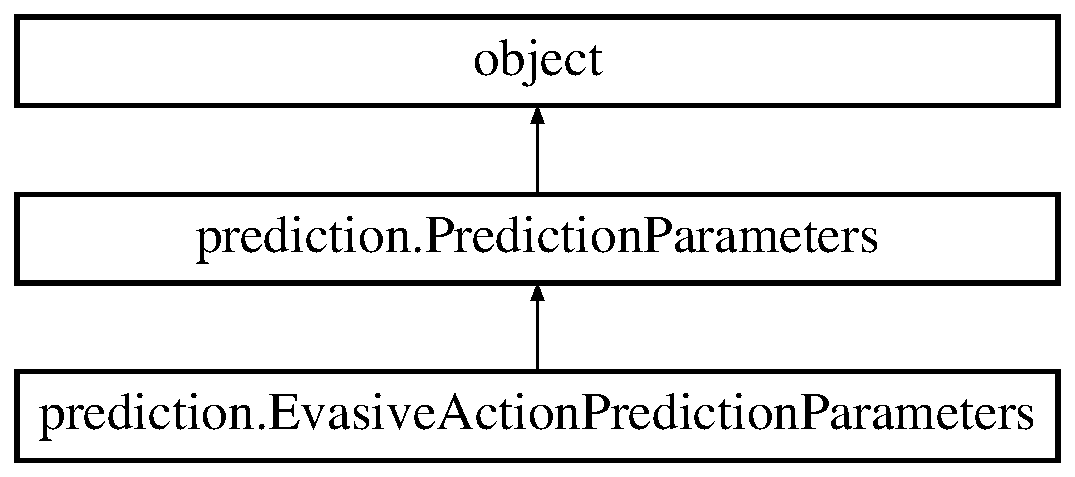
\includegraphics[height=3.000000cm]{classprediction_1_1EvasiveActionPredictionParameters}
\end{center}
\end{figure}
\subsubsection*{Public Member Functions}
\begin{DoxyCompactItemize}
\item 
def \hyperlink{classprediction_1_1EvasiveActionPredictionParameters_a98fc38dd46c873d5c2b0174353086870}{\-\_\-\-\_\-init\-\_\-\-\_\-}
\item 
def \hyperlink{classprediction_1_1EvasiveActionPredictionParameters_a61851834051a48bfcbf43a6310b2d3e3}{\-\_\-\-\_\-str\-\_\-\-\_\-}
\item 
def \hyperlink{classprediction_1_1EvasiveActionPredictionParameters_a3b6e8763a36f6549e547aba4a0c62982}{generate\-Predicted\-Trajectories}
\end{DoxyCompactItemize}
\subsubsection*{Public Attributes}
\begin{DoxyCompactItemize}
\item 
\hyperlink{classprediction_1_1EvasiveActionPredictionParameters_ace676c39fbf562303d7e9f2edf65d71c}{n\-Predicted\-Trajectories}
\item 
\hyperlink{classprediction_1_1EvasiveActionPredictionParameters_a998ff692327907d9b5f368fc5e3d906a}{use\-Features}
\item 
\hyperlink{classprediction_1_1EvasiveActionPredictionParameters_ab4638465c5d0cf8c4605b243d3f18ce9}{acceleration\-Distribution}
\item 
\hyperlink{classprediction_1_1EvasiveActionPredictionParameters_aee3f8965c1e1a9981a39c5626d61b022}{steering\-Distribution}
\end{DoxyCompactItemize}


\subsubsection{Constructor \& Destructor Documentation}
\hypertarget{classprediction_1_1EvasiveActionPredictionParameters_a98fc38dd46c873d5c2b0174353086870}{\index{prediction\-::\-Evasive\-Action\-Prediction\-Parameters@{prediction\-::\-Evasive\-Action\-Prediction\-Parameters}!\-\_\-\-\_\-init\-\_\-\-\_\-@{\-\_\-\-\_\-init\-\_\-\-\_\-}}
\index{\-\_\-\-\_\-init\-\_\-\-\_\-@{\-\_\-\-\_\-init\-\_\-\-\_\-}!prediction::EvasiveActionPredictionParameters@{prediction\-::\-Evasive\-Action\-Prediction\-Parameters}}
\paragraph[{\-\_\-\-\_\-init\-\_\-\-\_\-}]{\setlength{\rightskip}{0pt plus 5cm}def prediction.\-Evasive\-Action\-Prediction\-Parameters.\-\_\-\-\_\-init\-\_\-\-\_\- (
\begin{DoxyParamCaption}
\item[{}]{self, }
\item[{}]{max\-Speed, }
\item[{}]{n\-Predicted\-Trajectories, }
\item[{}]{acceleration\-Distribution, }
\item[{}]{steering\-Distribution, }
\item[{}]{use\-Features = {\ttfamily False}}
\end{DoxyParamCaption}
)}}\label{classprediction_1_1EvasiveActionPredictionParameters_a98fc38dd46c873d5c2b0174353086870}
\begin{DoxyVerb}Suggested acceleration distribution may not be symmetric, eg
lambda: random.triangular(self.minAcceleration, self.maxAcceleration, 0.)\end{DoxyVerb}
 

\subsubsection{Member Function Documentation}
\hypertarget{classprediction_1_1EvasiveActionPredictionParameters_a61851834051a48bfcbf43a6310b2d3e3}{\index{prediction\-::\-Evasive\-Action\-Prediction\-Parameters@{prediction\-::\-Evasive\-Action\-Prediction\-Parameters}!\-\_\-\-\_\-str\-\_\-\-\_\-@{\-\_\-\-\_\-str\-\_\-\-\_\-}}
\index{\-\_\-\-\_\-str\-\_\-\-\_\-@{\-\_\-\-\_\-str\-\_\-\-\_\-}!prediction::EvasiveActionPredictionParameters@{prediction\-::\-Evasive\-Action\-Prediction\-Parameters}}
\paragraph[{\-\_\-\-\_\-str\-\_\-\-\_\-}]{\setlength{\rightskip}{0pt plus 5cm}def prediction.\-Evasive\-Action\-Prediction\-Parameters.\-\_\-\-\_\-str\-\_\-\-\_\- (
\begin{DoxyParamCaption}
\item[{}]{self}
\end{DoxyParamCaption}
)}}\label{classprediction_1_1EvasiveActionPredictionParameters_a61851834051a48bfcbf43a6310b2d3e3}


References K\-L\-T\-Feature\-Tracking\-Parameters.\-max\-Acceleration, K\-L\-T\-Feature\-Tracking\-Parameters.\-max\-Steering, K\-L\-T\-Feature\-Tracking\-Parameters.\-min\-Acceleration, K\-L\-T\-Feature\-Tracking\-Parameters.\-n\-Predicted\-Trajectories, prediction.\-Normal\-Adaptation\-Prediction\-Parameters.\-n\-Predicted\-Trajectories, and prediction.\-Evasive\-Action\-Prediction\-Parameters.\-n\-Predicted\-Trajectories.

\hypertarget{classprediction_1_1EvasiveActionPredictionParameters_a3b6e8763a36f6549e547aba4a0c62982}{\index{prediction\-::\-Evasive\-Action\-Prediction\-Parameters@{prediction\-::\-Evasive\-Action\-Prediction\-Parameters}!generate\-Predicted\-Trajectories@{generate\-Predicted\-Trajectories}}
\index{generate\-Predicted\-Trajectories@{generate\-Predicted\-Trajectories}!prediction::EvasiveActionPredictionParameters@{prediction\-::\-Evasive\-Action\-Prediction\-Parameters}}
\paragraph[{generate\-Predicted\-Trajectories}]{\setlength{\rightskip}{0pt plus 5cm}def prediction.\-Evasive\-Action\-Prediction\-Parameters.\-generate\-Predicted\-Trajectories (
\begin{DoxyParamCaption}
\item[{}]{self, }
\item[{}]{obj, }
\item[{}]{instant}
\end{DoxyParamCaption}
)}}\label{classprediction_1_1EvasiveActionPredictionParameters_a3b6e8763a36f6549e547aba4a0c62982}


References prediction.\-Predicted\-Trajectory\-Random\-Control.\-acceleration\-Distribution, prediction.\-Normal\-Adaptation\-Prediction\-Parameters.\-acceleration\-Distribution, prediction.\-Evasive\-Action\-Prediction\-Parameters.\-acceleration\-Distribution, prediction.\-Predicted\-Trajectory\-Constant.\-max\-Speed, prediction.\-Predicted\-Trajectory\-Random\-Control.\-max\-Speed, prediction.\-Prediction\-Parameters.\-max\-Speed, K\-L\-T\-Feature\-Tracking\-Parameters.\-n\-Predicted\-Trajectories, prediction.\-Normal\-Adaptation\-Prediction\-Parameters.\-n\-Predicted\-Trajectories, prediction.\-Evasive\-Action\-Prediction\-Parameters.\-n\-Predicted\-Trajectories, prediction.\-Predicted\-Trajectory\-Random\-Control.\-steering\-Distribution, prediction.\-Normal\-Adaptation\-Prediction\-Parameters.\-steering\-Distribution, prediction.\-Evasive\-Action\-Prediction\-Parameters.\-steering\-Distribution, prediction.\-Normal\-Adaptation\-Prediction\-Parameters.\-use\-Features, and prediction.\-Evasive\-Action\-Prediction\-Parameters.\-use\-Features.



\subsubsection{Member Data Documentation}
\hypertarget{classprediction_1_1EvasiveActionPredictionParameters_ab4638465c5d0cf8c4605b243d3f18ce9}{\index{prediction\-::\-Evasive\-Action\-Prediction\-Parameters@{prediction\-::\-Evasive\-Action\-Prediction\-Parameters}!acceleration\-Distribution@{acceleration\-Distribution}}
\index{acceleration\-Distribution@{acceleration\-Distribution}!prediction::EvasiveActionPredictionParameters@{prediction\-::\-Evasive\-Action\-Prediction\-Parameters}}
\paragraph[{acceleration\-Distribution}]{\setlength{\rightskip}{0pt plus 5cm}prediction.\-Evasive\-Action\-Prediction\-Parameters.\-acceleration\-Distribution}}\label{classprediction_1_1EvasiveActionPredictionParameters_ab4638465c5d0cf8c4605b243d3f18ce9}
\hypertarget{classprediction_1_1EvasiveActionPredictionParameters_ace676c39fbf562303d7e9f2edf65d71c}{\index{prediction\-::\-Evasive\-Action\-Prediction\-Parameters@{prediction\-::\-Evasive\-Action\-Prediction\-Parameters}!n\-Predicted\-Trajectories@{n\-Predicted\-Trajectories}}
\index{n\-Predicted\-Trajectories@{n\-Predicted\-Trajectories}!prediction::EvasiveActionPredictionParameters@{prediction\-::\-Evasive\-Action\-Prediction\-Parameters}}
\paragraph[{n\-Predicted\-Trajectories}]{\setlength{\rightskip}{0pt plus 5cm}prediction.\-Evasive\-Action\-Prediction\-Parameters.\-n\-Predicted\-Trajectories}}\label{classprediction_1_1EvasiveActionPredictionParameters_ace676c39fbf562303d7e9f2edf65d71c}
\hypertarget{classprediction_1_1EvasiveActionPredictionParameters_aee3f8965c1e1a9981a39c5626d61b022}{\index{prediction\-::\-Evasive\-Action\-Prediction\-Parameters@{prediction\-::\-Evasive\-Action\-Prediction\-Parameters}!steering\-Distribution@{steering\-Distribution}}
\index{steering\-Distribution@{steering\-Distribution}!prediction::EvasiveActionPredictionParameters@{prediction\-::\-Evasive\-Action\-Prediction\-Parameters}}
\paragraph[{steering\-Distribution}]{\setlength{\rightskip}{0pt plus 5cm}prediction.\-Evasive\-Action\-Prediction\-Parameters.\-steering\-Distribution}}\label{classprediction_1_1EvasiveActionPredictionParameters_aee3f8965c1e1a9981a39c5626d61b022}
\hypertarget{classprediction_1_1EvasiveActionPredictionParameters_a998ff692327907d9b5f368fc5e3d906a}{\index{prediction\-::\-Evasive\-Action\-Prediction\-Parameters@{prediction\-::\-Evasive\-Action\-Prediction\-Parameters}!use\-Features@{use\-Features}}
\index{use\-Features@{use\-Features}!prediction::EvasiveActionPredictionParameters@{prediction\-::\-Evasive\-Action\-Prediction\-Parameters}}
\paragraph[{use\-Features}]{\setlength{\rightskip}{0pt plus 5cm}prediction.\-Evasive\-Action\-Prediction\-Parameters.\-use\-Features}}\label{classprediction_1_1EvasiveActionPredictionParameters_a998ff692327907d9b5f368fc5e3d906a}


The documentation for this class was generated from the following file\-:\begin{DoxyCompactItemize}
\item 
python/\hyperlink{prediction_8py}{prediction.\-py}\end{DoxyCompactItemize}

\hypertarget{classCatch_1_1ExceptionTranslatorRegistrar}{\subsection{Catch\-:\-:Exception\-Translator\-Registrar Class Reference}
\label{classCatch_1_1ExceptionTranslatorRegistrar}\index{Catch\-::\-Exception\-Translator\-Registrar@{Catch\-::\-Exception\-Translator\-Registrar}}
}


{\ttfamily \#include $<$catch.\-hpp$>$}

\subsubsection*{Public Member Functions}
\begin{DoxyCompactItemize}
\item 
{\footnotesize template$<$typename T $>$ }\\\hyperlink{classCatch_1_1ExceptionTranslatorRegistrar_aa73229de911f26b1df6c6c87c4d9e04e}{Exception\-Translator\-Registrar} (std\-::string($\ast$translate\-Function)(T \&))
\end{DoxyCompactItemize}


\subsubsection{Constructor \& Destructor Documentation}
\hypertarget{classCatch_1_1ExceptionTranslatorRegistrar_aa73229de911f26b1df6c6c87c4d9e04e}{\index{Catch\-::\-Exception\-Translator\-Registrar@{Catch\-::\-Exception\-Translator\-Registrar}!Exception\-Translator\-Registrar@{Exception\-Translator\-Registrar}}
\index{Exception\-Translator\-Registrar@{Exception\-Translator\-Registrar}!Catch::ExceptionTranslatorRegistrar@{Catch\-::\-Exception\-Translator\-Registrar}}
\paragraph[{Exception\-Translator\-Registrar}]{\setlength{\rightskip}{0pt plus 5cm}template$<$typename T $>$ Catch\-::\-Exception\-Translator\-Registrar\-::\-Exception\-Translator\-Registrar (
\begin{DoxyParamCaption}
\item[{std\-::string($\ast$)(T \&)}]{translate\-Function}
\end{DoxyParamCaption}
)\hspace{0.3cm}{\ttfamily [inline]}}}\label{classCatch_1_1ExceptionTranslatorRegistrar_aa73229de911f26b1df6c6c87c4d9e04e}


References Catch\-::get\-Current\-Context(), Catch\-::\-I\-Context\-::get\-Exception\-Translator\-Registry(), and Catch\-::\-I\-Exception\-Translator\-Registry\-::register\-Translator().



The documentation for this class was generated from the following file\-:\begin{DoxyCompactItemize}
\item 
include/\hyperlink{catch_8hpp}{catch.\-hpp}\end{DoxyCompactItemize}

\hypertarget{classCatch_1_1Expression}{\subsection{Catch\-:\-:Expression$<$ T $>$ Class Template Reference}
\label{classCatch_1_1Expression}\index{Catch\-::\-Expression$<$ T $>$@{Catch\-::\-Expression$<$ T $>$}}
}


{\ttfamily \#include $<$catch.\-hpp$>$}

\subsubsection*{Public Member Functions}
\begin{DoxyCompactItemize}
\item 
\hyperlink{classCatch_1_1Expression_ad5502009f1d9653ba09f4171c35528b4}{Expression} (\hyperlink{classCatch_1_1ResultInfoBuilder}{Result\-Info\-Builder} \&result, T lhs)
\item 
{\footnotesize template$<$typename Rhs\-T $>$ }\\\hyperlink{classCatch_1_1ResultInfoBuilder}{Result\-Info\-Builder} \& \hyperlink{classCatch_1_1Expression_ae6be91d91dea612743f3165caf5ea943}{operator==} (const Rhs\-T \&rhs)
\item 
{\footnotesize template$<$typename Rhs\-T $>$ }\\\hyperlink{classCatch_1_1ResultInfoBuilder}{Result\-Info\-Builder} \& \hyperlink{classCatch_1_1Expression_acd9e24e866370bda640156191f41be0c}{operator!=} (const Rhs\-T \&rhs)
\item 
{\footnotesize template$<$typename Rhs\-T $>$ }\\\hyperlink{classCatch_1_1ResultInfoBuilder}{Result\-Info\-Builder} \& \hyperlink{classCatch_1_1Expression_ac4cd605b13884865d9d2654f759b242b}{operator$<$} (const Rhs\-T \&rhs)
\item 
{\footnotesize template$<$typename Rhs\-T $>$ }\\\hyperlink{classCatch_1_1ResultInfoBuilder}{Result\-Info\-Builder} \& \hyperlink{classCatch_1_1Expression_a683e967108380ceb955dfc152c7874d0}{operator$>$} (const Rhs\-T \&rhs)
\item 
{\footnotesize template$<$typename Rhs\-T $>$ }\\\hyperlink{classCatch_1_1ResultInfoBuilder}{Result\-Info\-Builder} \& \hyperlink{classCatch_1_1Expression_ad7273b285b2d9ea81ac580ee9951eeac}{operator$<$=} (const Rhs\-T \&rhs)
\item 
{\footnotesize template$<$typename Rhs\-T $>$ }\\\hyperlink{classCatch_1_1ResultInfoBuilder}{Result\-Info\-Builder} \& \hyperlink{classCatch_1_1Expression_adfa8af4179fe39b8465a4b011d80432f}{operator$>$=} (const Rhs\-T \&rhs)
\item 
\hyperlink{classCatch_1_1ResultInfoBuilder}{Result\-Info\-Builder} \& \hyperlink{classCatch_1_1Expression_a83582006221d363d90cec0cb81dac716}{operator==} (bool rhs)
\item 
\hyperlink{classCatch_1_1ResultInfoBuilder}{Result\-Info\-Builder} \& \hyperlink{classCatch_1_1Expression_a67415524c7fb9d2c121f35d8f6a7c4ec}{operator!=} (bool rhs)
\item 
\hyperlink{classCatch_1_1Expression_af7c19481ee40f56a0ae9c274cb9e3baa}{operator Result\-Info\-Builder \&} ()
\item 
{\footnotesize template$<$typename Rhs\-T $>$ }\\S\-T\-A\-T\-I\-C\-\_\-\-A\-S\-S\-E\-R\-T\-\_\-\-Expression\-\_\-\-Too\-\_\-\-Complex\-\_\-\-Please\-\_\-\-Rewrite\-\_\-\-As\-\_\-\-Binary\-\_\-\-Comparison \& \hyperlink{classCatch_1_1Expression_a7cd07f3cc77303310eaedb0431a54ff3}{operator+} (const Rhs\-T \&)
\item 
{\footnotesize template$<$typename Rhs\-T $>$ }\\S\-T\-A\-T\-I\-C\-\_\-\-A\-S\-S\-E\-R\-T\-\_\-\-Expression\-\_\-\-Too\-\_\-\-Complex\-\_\-\-Please\-\_\-\-Rewrite\-\_\-\-As\-\_\-\-Binary\-\_\-\-Comparison \& \hyperlink{classCatch_1_1Expression_ad8b6189cc41070b597c073e0c23e48af}{operator-\/} (const Rhs\-T \&)
\end{DoxyCompactItemize}


\subsubsection{Constructor \& Destructor Documentation}
\hypertarget{classCatch_1_1Expression_ad5502009f1d9653ba09f4171c35528b4}{\index{Catch\-::\-Expression@{Catch\-::\-Expression}!Expression@{Expression}}
\index{Expression@{Expression}!Catch::Expression@{Catch\-::\-Expression}}
\paragraph[{Expression}]{\setlength{\rightskip}{0pt plus 5cm}template$<$typename T$>$ {\bf Catch\-::\-Expression}$<$ T $>$\-::{\bf Expression} (
\begin{DoxyParamCaption}
\item[{{\bf Result\-Info\-Builder} \&}]{result, }
\item[{T}]{lhs}
\end{DoxyParamCaption}
)\hspace{0.3cm}{\ttfamily [inline]}}}\label{classCatch_1_1Expression_ad5502009f1d9653ba09f4171c35528b4}


\subsubsection{Member Function Documentation}
\hypertarget{classCatch_1_1Expression_af7c19481ee40f56a0ae9c274cb9e3baa}{\index{Catch\-::\-Expression@{Catch\-::\-Expression}!operator Result\-Info\-Builder \&@{operator Result\-Info\-Builder \&}}
\index{operator Result\-Info\-Builder \&@{operator Result\-Info\-Builder \&}!Catch::Expression@{Catch\-::\-Expression}}
\paragraph[{operator Result\-Info\-Builder \&}]{\setlength{\rightskip}{0pt plus 5cm}template$<$typename T$>$ {\bf Catch\-::\-Expression}$<$ T $>$\-::operator {\bf Result\-Info\-Builder} \& (
\begin{DoxyParamCaption}
{}
\end{DoxyParamCaption}
)\hspace{0.3cm}{\ttfamily [inline]}}}\label{classCatch_1_1Expression_af7c19481ee40f56a0ae9c274cb9e3baa}
\hypertarget{classCatch_1_1Expression_acd9e24e866370bda640156191f41be0c}{\index{Catch\-::\-Expression@{Catch\-::\-Expression}!operator!=@{operator!=}}
\index{operator!=@{operator!=}!Catch::Expression@{Catch\-::\-Expression}}
\paragraph[{operator!=}]{\setlength{\rightskip}{0pt plus 5cm}template$<$typename T$>$ template$<$typename Rhs\-T $>$ {\bf Result\-Info\-Builder}\& {\bf Catch\-::\-Expression}$<$ T $>$\-::operator!= (
\begin{DoxyParamCaption}
\item[{const Rhs\-T \&}]{rhs}
\end{DoxyParamCaption}
)\hspace{0.3cm}{\ttfamily [inline]}}}\label{classCatch_1_1Expression_acd9e24e866370bda640156191f41be0c}


References Catch\-::\-Internal\-::\-Is\-Not\-Equal\-To.

\hypertarget{classCatch_1_1Expression_a67415524c7fb9d2c121f35d8f6a7c4ec}{\index{Catch\-::\-Expression@{Catch\-::\-Expression}!operator!=@{operator!=}}
\index{operator!=@{operator!=}!Catch::Expression@{Catch\-::\-Expression}}
\paragraph[{operator!=}]{\setlength{\rightskip}{0pt plus 5cm}template$<$typename T$>$ {\bf Result\-Info\-Builder}\& {\bf Catch\-::\-Expression}$<$ T $>$\-::operator!= (
\begin{DoxyParamCaption}
\item[{bool}]{rhs}
\end{DoxyParamCaption}
)\hspace{0.3cm}{\ttfamily [inline]}}}\label{classCatch_1_1Expression_a67415524c7fb9d2c121f35d8f6a7c4ec}


References Catch\-::\-Internal\-::\-Is\-Not\-Equal\-To.

\hypertarget{classCatch_1_1Expression_a7cd07f3cc77303310eaedb0431a54ff3}{\index{Catch\-::\-Expression@{Catch\-::\-Expression}!operator+@{operator+}}
\index{operator+@{operator+}!Catch::Expression@{Catch\-::\-Expression}}
\paragraph[{operator+}]{\setlength{\rightskip}{0pt plus 5cm}template$<$typename T$>$ template$<$typename Rhs\-T $>$ S\-T\-A\-T\-I\-C\-\_\-\-A\-S\-S\-E\-R\-T\-\_\-\-Expression\-\_\-\-Too\-\_\-\-Complex\-\_\-\-Please\-\_\-\-Rewrite\-\_\-\-As\-\_\-\-Binary\-\_\-\-Comparison\& {\bf Catch\-::\-Expression}$<$ T $>$\-::operator+ (
\begin{DoxyParamCaption}
\item[{const Rhs\-T \&}]{}
\end{DoxyParamCaption}
)}}\label{classCatch_1_1Expression_a7cd07f3cc77303310eaedb0431a54ff3}
\hypertarget{classCatch_1_1Expression_ad8b6189cc41070b597c073e0c23e48af}{\index{Catch\-::\-Expression@{Catch\-::\-Expression}!operator-\/@{operator-\/}}
\index{operator-\/@{operator-\/}!Catch::Expression@{Catch\-::\-Expression}}
\paragraph[{operator-\/}]{\setlength{\rightskip}{0pt plus 5cm}template$<$typename T$>$ template$<$typename Rhs\-T $>$ S\-T\-A\-T\-I\-C\-\_\-\-A\-S\-S\-E\-R\-T\-\_\-\-Expression\-\_\-\-Too\-\_\-\-Complex\-\_\-\-Please\-\_\-\-Rewrite\-\_\-\-As\-\_\-\-Binary\-\_\-\-Comparison\& {\bf Catch\-::\-Expression}$<$ T $>$\-::operator-\/ (
\begin{DoxyParamCaption}
\item[{const Rhs\-T \&}]{}
\end{DoxyParamCaption}
)}}\label{classCatch_1_1Expression_ad8b6189cc41070b597c073e0c23e48af}
\hypertarget{classCatch_1_1Expression_ac4cd605b13884865d9d2654f759b242b}{\index{Catch\-::\-Expression@{Catch\-::\-Expression}!operator$<$@{operator$<$}}
\index{operator$<$@{operator$<$}!Catch::Expression@{Catch\-::\-Expression}}
\paragraph[{operator$<$}]{\setlength{\rightskip}{0pt plus 5cm}template$<$typename T$>$ template$<$typename Rhs\-T $>$ {\bf Result\-Info\-Builder}\& {\bf Catch\-::\-Expression}$<$ T $>$\-::operator$<$ (
\begin{DoxyParamCaption}
\item[{const Rhs\-T \&}]{rhs}
\end{DoxyParamCaption}
)\hspace{0.3cm}{\ttfamily [inline]}}}\label{classCatch_1_1Expression_ac4cd605b13884865d9d2654f759b242b}


References Catch\-::\-Internal\-::\-Is\-Less\-Than.

\hypertarget{classCatch_1_1Expression_ad7273b285b2d9ea81ac580ee9951eeac}{\index{Catch\-::\-Expression@{Catch\-::\-Expression}!operator$<$=@{operator$<$=}}
\index{operator$<$=@{operator$<$=}!Catch::Expression@{Catch\-::\-Expression}}
\paragraph[{operator$<$=}]{\setlength{\rightskip}{0pt plus 5cm}template$<$typename T$>$ template$<$typename Rhs\-T $>$ {\bf Result\-Info\-Builder}\& {\bf Catch\-::\-Expression}$<$ T $>$\-::operator$<$= (
\begin{DoxyParamCaption}
\item[{const Rhs\-T \&}]{rhs}
\end{DoxyParamCaption}
)\hspace{0.3cm}{\ttfamily [inline]}}}\label{classCatch_1_1Expression_ad7273b285b2d9ea81ac580ee9951eeac}


References Catch\-::\-Internal\-::\-Is\-Less\-Than\-Or\-Equal\-To.

\hypertarget{classCatch_1_1Expression_ae6be91d91dea612743f3165caf5ea943}{\index{Catch\-::\-Expression@{Catch\-::\-Expression}!operator==@{operator==}}
\index{operator==@{operator==}!Catch::Expression@{Catch\-::\-Expression}}
\paragraph[{operator==}]{\setlength{\rightskip}{0pt plus 5cm}template$<$typename T$>$ template$<$typename Rhs\-T $>$ {\bf Result\-Info\-Builder}\& {\bf Catch\-::\-Expression}$<$ T $>$\-::operator== (
\begin{DoxyParamCaption}
\item[{const Rhs\-T \&}]{rhs}
\end{DoxyParamCaption}
)\hspace{0.3cm}{\ttfamily [inline]}}}\label{classCatch_1_1Expression_ae6be91d91dea612743f3165caf5ea943}


References Catch\-::\-Internal\-::\-Is\-Equal\-To.

\hypertarget{classCatch_1_1Expression_a83582006221d363d90cec0cb81dac716}{\index{Catch\-::\-Expression@{Catch\-::\-Expression}!operator==@{operator==}}
\index{operator==@{operator==}!Catch::Expression@{Catch\-::\-Expression}}
\paragraph[{operator==}]{\setlength{\rightskip}{0pt plus 5cm}template$<$typename T$>$ {\bf Result\-Info\-Builder}\& {\bf Catch\-::\-Expression}$<$ T $>$\-::operator== (
\begin{DoxyParamCaption}
\item[{bool}]{rhs}
\end{DoxyParamCaption}
)\hspace{0.3cm}{\ttfamily [inline]}}}\label{classCatch_1_1Expression_a83582006221d363d90cec0cb81dac716}


References Catch\-::\-Internal\-::\-Is\-Equal\-To.

\hypertarget{classCatch_1_1Expression_a683e967108380ceb955dfc152c7874d0}{\index{Catch\-::\-Expression@{Catch\-::\-Expression}!operator$>$@{operator$>$}}
\index{operator$>$@{operator$>$}!Catch::Expression@{Catch\-::\-Expression}}
\paragraph[{operator$>$}]{\setlength{\rightskip}{0pt plus 5cm}template$<$typename T$>$ template$<$typename Rhs\-T $>$ {\bf Result\-Info\-Builder}\& {\bf Catch\-::\-Expression}$<$ T $>$\-::operator$>$ (
\begin{DoxyParamCaption}
\item[{const Rhs\-T \&}]{rhs}
\end{DoxyParamCaption}
)\hspace{0.3cm}{\ttfamily [inline]}}}\label{classCatch_1_1Expression_a683e967108380ceb955dfc152c7874d0}


References Catch\-::\-Internal\-::\-Is\-Greater\-Than.

\hypertarget{classCatch_1_1Expression_adfa8af4179fe39b8465a4b011d80432f}{\index{Catch\-::\-Expression@{Catch\-::\-Expression}!operator$>$=@{operator$>$=}}
\index{operator$>$=@{operator$>$=}!Catch::Expression@{Catch\-::\-Expression}}
\paragraph[{operator$>$=}]{\setlength{\rightskip}{0pt plus 5cm}template$<$typename T$>$ template$<$typename Rhs\-T $>$ {\bf Result\-Info\-Builder}\& {\bf Catch\-::\-Expression}$<$ T $>$\-::operator$>$= (
\begin{DoxyParamCaption}
\item[{const Rhs\-T \&}]{rhs}
\end{DoxyParamCaption}
)\hspace{0.3cm}{\ttfamily [inline]}}}\label{classCatch_1_1Expression_adfa8af4179fe39b8465a4b011d80432f}


References Catch\-::\-Internal\-::\-Is\-Greater\-Than\-Or\-Equal\-To.



The documentation for this class was generated from the following file\-:\begin{DoxyCompactItemize}
\item 
include/\hyperlink{catch_8hpp}{catch.\-hpp}\end{DoxyCompactItemize}

\hypertarget{classCatch_1_1ExpressionBuilder}{\subsection{Catch\-:\-:Expression\-Builder Class Reference}
\label{classCatch_1_1ExpressionBuilder}\index{Catch\-::\-Expression\-Builder@{Catch\-::\-Expression\-Builder}}
}


{\ttfamily \#include $<$catch.\-hpp$>$}

\subsubsection*{Public Member Functions}
\begin{DoxyCompactItemize}
\item 
\hyperlink{classCatch_1_1ExpressionBuilder_ace5fb1d3d95924fd928443fb8c2614d6}{Expression\-Builder} (const \hyperlink{structCatch_1_1SourceLineInfo}{Source\-Line\-Info} \&line\-Info, const char $\ast$macro\-Name, const char $\ast$expr=\char`\"{}\char`\"{}, bool is\-Not=false)
\item 
{\footnotesize template$<$typename T $>$ }\\\hyperlink{classCatch_1_1Expression}{Expression}$<$ const T \& $>$ \hyperlink{classCatch_1_1ExpressionBuilder_a3af0b2041ebfab8c0c05d4e65102bb6e}{operator-\/$>$$\ast$} (const T \&operand)
\item 
\hyperlink{classCatch_1_1Expression}{Expression}$<$ bool $>$ \hyperlink{classCatch_1_1ExpressionBuilder_a5c783bea5d398fd36a351f758349f317}{operator-\/$>$$\ast$} (bool value)
\item 
{\footnotesize template$<$typename T $>$ }\\\hyperlink{classCatch_1_1ExpressionBuilder}{Expression\-Builder} \& \hyperlink{classCatch_1_1ExpressionBuilder_a0ec28bcd4789a85c20543358087cad4e}{operator$<$$<$} (const T \&value)
\item 
{\footnotesize template$<$typename Matcher\-T , typename Arg\-T $>$ }\\\hyperlink{classCatch_1_1ExpressionBuilder}{Expression\-Builder} \& \hyperlink{classCatch_1_1ExpressionBuilder_a24b9ddd2dc8bd1ce02d9db614f1de490}{accept\-Matcher} (const Matcher\-T \&matcher, const Arg\-T \&arg, const std\-::string \&matcher\-Call\-As\-String)
\item 
{\footnotesize template$<$typename Matcher\-T , typename Arg\-T $>$ }\\\hyperlink{classCatch_1_1ExpressionBuilder}{Expression\-Builder} \& \hyperlink{classCatch_1_1ExpressionBuilder_a72f02a5d86ab6293884bf3196eb56aa7}{accept\-Matcher} (const Matcher\-T \&matcher, Arg\-T $\ast$arg, const std\-::string \&matcher\-Call\-As\-String)
\item 
\hyperlink{classCatch_1_1ExpressionBuilder}{Expression\-Builder} \& \hyperlink{classCatch_1_1ExpressionBuilder_a35db86c0b9cf13cec57f1cd0fbb80100}{set\-Result\-Type} (\hyperlink{structCatch_1_1ResultWas_a624e1ee3661fcf6094ceef1f654601ef}{Result\-Was\-::\-Of\-Type} result\-Type)
\item 
\hyperlink{classCatch_1_1ExpressionBuilder_ab7c53debf1bfd505ae404665363248fe}{operator Result\-Info\-Builder \&} ()
\end{DoxyCompactItemize}


\subsubsection{Constructor \& Destructor Documentation}
\hypertarget{classCatch_1_1ExpressionBuilder_ace5fb1d3d95924fd928443fb8c2614d6}{\index{Catch\-::\-Expression\-Builder@{Catch\-::\-Expression\-Builder}!Expression\-Builder@{Expression\-Builder}}
\index{Expression\-Builder@{Expression\-Builder}!Catch::ExpressionBuilder@{Catch\-::\-Expression\-Builder}}
\paragraph[{Expression\-Builder}]{\setlength{\rightskip}{0pt plus 5cm}Catch\-::\-Expression\-Builder\-::\-Expression\-Builder (
\begin{DoxyParamCaption}
\item[{const {\bf Source\-Line\-Info} \&}]{line\-Info, }
\item[{const char $\ast$}]{macro\-Name, }
\item[{const char $\ast$}]{expr = {\ttfamily \char`\"{}\char`\"{}}, }
\item[{bool}]{is\-Not = {\ttfamily false}}
\end{DoxyParamCaption}
)\hspace{0.3cm}{\ttfamily [inline]}}}\label{classCatch_1_1ExpressionBuilder_ace5fb1d3d95924fd928443fb8c2614d6}


\subsubsection{Member Function Documentation}
\hypertarget{classCatch_1_1ExpressionBuilder_a24b9ddd2dc8bd1ce02d9db614f1de490}{\index{Catch\-::\-Expression\-Builder@{Catch\-::\-Expression\-Builder}!accept\-Matcher@{accept\-Matcher}}
\index{accept\-Matcher@{accept\-Matcher}!Catch::ExpressionBuilder@{Catch\-::\-Expression\-Builder}}
\paragraph[{accept\-Matcher}]{\setlength{\rightskip}{0pt plus 5cm}template$<$typename Matcher\-T , typename Arg\-T $>$ {\bf Expression\-Builder}\& Catch\-::\-Expression\-Builder\-::accept\-Matcher (
\begin{DoxyParamCaption}
\item[{const Matcher\-T \&}]{matcher, }
\item[{const Arg\-T \&}]{arg, }
\item[{const std\-::string \&}]{matcher\-Call\-As\-String}
\end{DoxyParamCaption}
)\hspace{0.3cm}{\ttfamily [inline]}}}\label{classCatch_1_1ExpressionBuilder_a24b9ddd2dc8bd1ce02d9db614f1de490}


References Catch\-::\-Result\-Was\-::\-Expression\-Failed, Catch\-::\-Result\-Was\-::\-Ok, Catch\-::\-Result\-Info\-Builder\-::set\-Lhs(), Catch\-::\-Result\-Info\-Builder\-::set\-Op(), Catch\-::\-Result\-Info\-Builder\-::set\-Result\-Type(), Catch\-::\-Result\-Info\-Builder\-::set\-Rhs(), and Catch\-::to\-String().

\hypertarget{classCatch_1_1ExpressionBuilder_a72f02a5d86ab6293884bf3196eb56aa7}{\index{Catch\-::\-Expression\-Builder@{Catch\-::\-Expression\-Builder}!accept\-Matcher@{accept\-Matcher}}
\index{accept\-Matcher@{accept\-Matcher}!Catch::ExpressionBuilder@{Catch\-::\-Expression\-Builder}}
\paragraph[{accept\-Matcher}]{\setlength{\rightskip}{0pt plus 5cm}template$<$typename Matcher\-T , typename Arg\-T $>$ {\bf Expression\-Builder}\& Catch\-::\-Expression\-Builder\-::accept\-Matcher (
\begin{DoxyParamCaption}
\item[{const Matcher\-T \&}]{matcher, }
\item[{Arg\-T $\ast$}]{arg, }
\item[{const std\-::string \&}]{matcher\-Call\-As\-String}
\end{DoxyParamCaption}
)\hspace{0.3cm}{\ttfamily [inline]}}}\label{classCatch_1_1ExpressionBuilder_a72f02a5d86ab6293884bf3196eb56aa7}


References Catch\-::\-Result\-Was\-::\-Expression\-Failed, Catch\-::\-Result\-Was\-::\-Ok, Catch\-::\-Result\-Info\-Builder\-::set\-Lhs(), Catch\-::\-Result\-Info\-Builder\-::set\-Op(), Catch\-::\-Result\-Info\-Builder\-::set\-Result\-Type(), Catch\-::\-Result\-Info\-Builder\-::set\-Rhs(), and Catch\-::to\-String().

\hypertarget{classCatch_1_1ExpressionBuilder_ab7c53debf1bfd505ae404665363248fe}{\index{Catch\-::\-Expression\-Builder@{Catch\-::\-Expression\-Builder}!operator Result\-Info\-Builder \&@{operator Result\-Info\-Builder \&}}
\index{operator Result\-Info\-Builder \&@{operator Result\-Info\-Builder \&}!Catch::ExpressionBuilder@{Catch\-::\-Expression\-Builder}}
\paragraph[{operator Result\-Info\-Builder \&}]{\setlength{\rightskip}{0pt plus 5cm}Catch\-::\-Expression\-Builder\-::operator {\bf Result\-Info\-Builder} \& (
\begin{DoxyParamCaption}
{}
\end{DoxyParamCaption}
)\hspace{0.3cm}{\ttfamily [inline]}}}\label{classCatch_1_1ExpressionBuilder_ab7c53debf1bfd505ae404665363248fe}


References Catch\-::\-Result\-Info\-Builder\-::set\-Message().

\hypertarget{classCatch_1_1ExpressionBuilder_a3af0b2041ebfab8c0c05d4e65102bb6e}{\index{Catch\-::\-Expression\-Builder@{Catch\-::\-Expression\-Builder}!operator-\/$>$$\ast$@{operator-\/$>$$\ast$}}
\index{operator-\/$>$$\ast$@{operator-\/$>$$\ast$}!Catch::ExpressionBuilder@{Catch\-::\-Expression\-Builder}}
\paragraph[{operator-\/$>$$\ast$}]{\setlength{\rightskip}{0pt plus 5cm}template$<$typename T $>$ {\bf Expression}$<$const T\&$>$ Catch\-::\-Expression\-Builder\-::operator-\/$>$$\ast$ (
\begin{DoxyParamCaption}
\item[{const T \&}]{operand}
\end{DoxyParamCaption}
)\hspace{0.3cm}{\ttfamily [inline]}}}\label{classCatch_1_1ExpressionBuilder_a3af0b2041ebfab8c0c05d4e65102bb6e}
\hypertarget{classCatch_1_1ExpressionBuilder_a5c783bea5d398fd36a351f758349f317}{\index{Catch\-::\-Expression\-Builder@{Catch\-::\-Expression\-Builder}!operator-\/$>$$\ast$@{operator-\/$>$$\ast$}}
\index{operator-\/$>$$\ast$@{operator-\/$>$$\ast$}!Catch::ExpressionBuilder@{Catch\-::\-Expression\-Builder}}
\paragraph[{operator-\/$>$$\ast$}]{\setlength{\rightskip}{0pt plus 5cm}{\bf Expression}$<$bool$>$ Catch\-::\-Expression\-Builder\-::operator-\/$>$$\ast$ (
\begin{DoxyParamCaption}
\item[{bool}]{value}
\end{DoxyParamCaption}
)\hspace{0.3cm}{\ttfamily [inline]}}}\label{classCatch_1_1ExpressionBuilder_a5c783bea5d398fd36a351f758349f317}
\hypertarget{classCatch_1_1ExpressionBuilder_a0ec28bcd4789a85c20543358087cad4e}{\index{Catch\-::\-Expression\-Builder@{Catch\-::\-Expression\-Builder}!operator$<$$<$@{operator$<$$<$}}
\index{operator$<$$<$@{operator$<$$<$}!Catch::ExpressionBuilder@{Catch\-::\-Expression\-Builder}}
\paragraph[{operator$<$$<$}]{\setlength{\rightskip}{0pt plus 5cm}template$<$typename T $>$ {\bf Expression\-Builder}\& Catch\-::\-Expression\-Builder\-::operator$<$$<$ (
\begin{DoxyParamCaption}
\item[{const T \&}]{value}
\end{DoxyParamCaption}
)\hspace{0.3cm}{\ttfamily [inline]}}}\label{classCatch_1_1ExpressionBuilder_a0ec28bcd4789a85c20543358087cad4e}


References Catch\-::to\-String().

\hypertarget{classCatch_1_1ExpressionBuilder_a35db86c0b9cf13cec57f1cd0fbb80100}{\index{Catch\-::\-Expression\-Builder@{Catch\-::\-Expression\-Builder}!set\-Result\-Type@{set\-Result\-Type}}
\index{set\-Result\-Type@{set\-Result\-Type}!Catch::ExpressionBuilder@{Catch\-::\-Expression\-Builder}}
\paragraph[{set\-Result\-Type}]{\setlength{\rightskip}{0pt plus 5cm}{\bf Expression\-Builder}\& Catch\-::\-Expression\-Builder\-::set\-Result\-Type (
\begin{DoxyParamCaption}
\item[{{\bf Result\-Was\-::\-Of\-Type}}]{result\-Type}
\end{DoxyParamCaption}
)\hspace{0.3cm}{\ttfamily [inline]}}}\label{classCatch_1_1ExpressionBuilder_a35db86c0b9cf13cec57f1cd0fbb80100}


References Catch\-::\-Result\-Info\-Builder\-::set\-Result\-Type().



The documentation for this class was generated from the following file\-:\begin{DoxyCompactItemize}
\item 
include/\hyperlink{catch_8hpp}{catch.\-hpp}\end{DoxyCompactItemize}

\hypertarget{classstorage_1_1FakeSecHead}{\subsection{storage.\-Fake\-Sec\-Head Class Reference}
\label{classstorage_1_1FakeSecHead}\index{storage.\-Fake\-Sec\-Head@{storage.\-Fake\-Sec\-Head}}
}
Inheritance diagram for storage.\-Fake\-Sec\-Head\-:\begin{figure}[H]
\begin{center}
\leavevmode
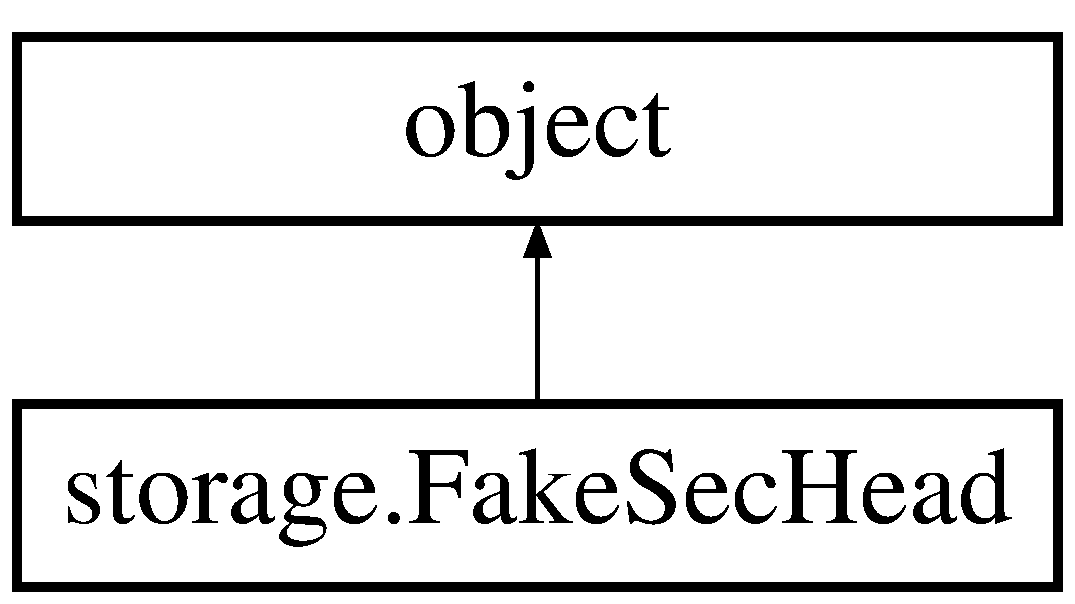
\includegraphics[height=2.000000cm]{classstorage_1_1FakeSecHead}
\end{center}
\end{figure}
\subsubsection*{Public Member Functions}
\begin{DoxyCompactItemize}
\item 
def \hyperlink{classstorage_1_1FakeSecHead_a6a57eb1adfb97de7d6246de6f3742226}{\-\_\-\-\_\-init\-\_\-\-\_\-}
\item 
def \hyperlink{classstorage_1_1FakeSecHead_a419fee3fa1ce40fc89d8743829e7eb45}{readline}
\end{DoxyCompactItemize}
\subsubsection*{Public Attributes}
\begin{DoxyCompactItemize}
\item 
\hyperlink{classstorage_1_1FakeSecHead_a568fc1a21d55931188b7dbb77f93b094}{fp}
\item 
\hyperlink{classstorage_1_1FakeSecHead_a34480f5cc048c82a51c460155a64aad1}{sechead}
\end{DoxyCompactItemize}


\subsubsection{Detailed Description}
\begin{DoxyVerb}Add fake section header [asection]

from http://stackoverflow.com/questions/2819696/parsing-properties-file-in-python/2819788#2819788
use read_file in Python 3.2+
\end{DoxyVerb}
 

\subsubsection{Constructor \& Destructor Documentation}
\hypertarget{classstorage_1_1FakeSecHead_a6a57eb1adfb97de7d6246de6f3742226}{\index{storage\-::\-Fake\-Sec\-Head@{storage\-::\-Fake\-Sec\-Head}!\-\_\-\-\_\-init\-\_\-\-\_\-@{\-\_\-\-\_\-init\-\_\-\-\_\-}}
\index{\-\_\-\-\_\-init\-\_\-\-\_\-@{\-\_\-\-\_\-init\-\_\-\-\_\-}!storage::FakeSecHead@{storage\-::\-Fake\-Sec\-Head}}
\paragraph[{\-\_\-\-\_\-init\-\_\-\-\_\-}]{\setlength{\rightskip}{0pt plus 5cm}def storage.\-Fake\-Sec\-Head.\-\_\-\-\_\-init\-\_\-\-\_\- (
\begin{DoxyParamCaption}
\item[{}]{self, }
\item[{}]{fp}
\end{DoxyParamCaption}
)}}\label{classstorage_1_1FakeSecHead_a6a57eb1adfb97de7d6246de6f3742226}


\subsubsection{Member Function Documentation}
\hypertarget{classstorage_1_1FakeSecHead_a419fee3fa1ce40fc89d8743829e7eb45}{\index{storage\-::\-Fake\-Sec\-Head@{storage\-::\-Fake\-Sec\-Head}!readline@{readline}}
\index{readline@{readline}!storage::FakeSecHead@{storage\-::\-Fake\-Sec\-Head}}
\paragraph[{readline}]{\setlength{\rightskip}{0pt plus 5cm}def storage.\-Fake\-Sec\-Head.\-readline (
\begin{DoxyParamCaption}
\item[{}]{self}
\end{DoxyParamCaption}
)}}\label{classstorage_1_1FakeSecHead_a419fee3fa1ce40fc89d8743829e7eb45}


References storage.\-Fake\-Sec\-Head.\-sechead.



\subsubsection{Member Data Documentation}
\hypertarget{classstorage_1_1FakeSecHead_a568fc1a21d55931188b7dbb77f93b094}{\index{storage\-::\-Fake\-Sec\-Head@{storage\-::\-Fake\-Sec\-Head}!fp@{fp}}
\index{fp@{fp}!storage::FakeSecHead@{storage\-::\-Fake\-Sec\-Head}}
\paragraph[{fp}]{\setlength{\rightskip}{0pt plus 5cm}storage.\-Fake\-Sec\-Head.\-fp}}\label{classstorage_1_1FakeSecHead_a568fc1a21d55931188b7dbb77f93b094}
\hypertarget{classstorage_1_1FakeSecHead_a34480f5cc048c82a51c460155a64aad1}{\index{storage\-::\-Fake\-Sec\-Head@{storage\-::\-Fake\-Sec\-Head}!sechead@{sechead}}
\index{sechead@{sechead}!storage::FakeSecHead@{storage\-::\-Fake\-Sec\-Head}}
\paragraph[{sechead}]{\setlength{\rightskip}{0pt plus 5cm}storage.\-Fake\-Sec\-Head.\-sechead}}\label{classstorage_1_1FakeSecHead_a34480f5cc048c82a51c460155a64aad1}


The documentation for this class was generated from the following file\-:\begin{DoxyCompactItemize}
\item 
python/\hyperlink{storage_8py}{storage.\-py}\end{DoxyCompactItemize}

\hypertarget{structFeatureGraph_1_1FeatureConnection}{\subsection{Feature\-Graph\-:\-:Feature\-Connection Struct Reference}
\label{structFeatureGraph_1_1FeatureConnection}\index{Feature\-Graph\-::\-Feature\-Connection@{Feature\-Graph\-::\-Feature\-Connection}}
}


{\ttfamily \#include $<$Motion.\-hpp$>$}

\subsubsection*{Public Attributes}
\begin{DoxyCompactItemize}
\item 
float \hyperlink{structFeatureGraph_1_1FeatureConnection_ad19c4e45cfeb673ca554081eb593958e}{min\-Distance}
\item 
float \hyperlink{structFeatureGraph_1_1FeatureConnection_ae327f4ab6ac124456d19a95aa2221ad8}{max\-Distance}
\end{DoxyCompactItemize}


\subsubsection{Member Data Documentation}
\hypertarget{structFeatureGraph_1_1FeatureConnection_ae327f4ab6ac124456d19a95aa2221ad8}{\index{Feature\-Graph\-::\-Feature\-Connection@{Feature\-Graph\-::\-Feature\-Connection}!max\-Distance@{max\-Distance}}
\index{max\-Distance@{max\-Distance}!FeatureGraph::FeatureConnection@{Feature\-Graph\-::\-Feature\-Connection}}
\paragraph[{max\-Distance}]{\setlength{\rightskip}{0pt plus 5cm}float Feature\-Graph\-::\-Feature\-Connection\-::max\-Distance}}\label{structFeatureGraph_1_1FeatureConnection_ae327f4ab6ac124456d19a95aa2221ad8}
\hypertarget{structFeatureGraph_1_1FeatureConnection_ad19c4e45cfeb673ca554081eb593958e}{\index{Feature\-Graph\-::\-Feature\-Connection@{Feature\-Graph\-::\-Feature\-Connection}!min\-Distance@{min\-Distance}}
\index{min\-Distance@{min\-Distance}!FeatureGraph::FeatureConnection@{Feature\-Graph\-::\-Feature\-Connection}}
\paragraph[{min\-Distance}]{\setlength{\rightskip}{0pt plus 5cm}float Feature\-Graph\-::\-Feature\-Connection\-::min\-Distance}}\label{structFeatureGraph_1_1FeatureConnection_ad19c4e45cfeb673ca554081eb593958e}


The documentation for this struct was generated from the following file\-:\begin{DoxyCompactItemize}
\item 
include/\hyperlink{Motion_8hpp}{Motion.\-hpp}\end{DoxyCompactItemize}

\hypertarget{classFeatureGraph}{\subsection{Feature\-Graph Class Reference}
\label{classFeatureGraph}\index{Feature\-Graph@{Feature\-Graph}}
}


{\ttfamily \#include $<$Motion.\-hpp$>$}

\subsubsection*{Classes}
\begin{DoxyCompactItemize}
\item 
struct \hyperlink{structFeatureGraph_1_1FeatureConnection}{Feature\-Connection}
\item 
struct \hyperlink{structFeatureGraph_1_1VertexInformation}{Vertex\-Information}
\end{DoxyCompactItemize}
\subsubsection*{Public Types}
\begin{DoxyCompactItemize}
\item 
typedef \\*
Undirected\-Graph\-::vertex\-\_\-descriptor \hyperlink{classFeatureGraph_ab85a700fea1a3a494db459c0f8277844}{vertex\-\_\-descriptor}
\end{DoxyCompactItemize}
\subsubsection*{Public Member Functions}
\begin{DoxyCompactItemize}
\item 
\hyperlink{classFeatureGraph_a388051116011290dbf5e8e613c3eb848}{Feature\-Graph} (float \-\_\-connection\-Distance, float \-\_\-segmentation\-Distance, unsigned int \-\_\-min\-Feature\-Time, float \-\_\-min\-N\-Features\-Per\-Group)
\item 
void \hyperlink{classFeatureGraph_a557fa8ecb18a4941e53f563b886c3183}{add\-Feature} (const \hyperlink{Motion_8hpp_a86ae4681c45e5385d5543cff332f56f4}{Feature\-Trajectory\-Ptr} \&ft)
\item 
void \hyperlink{classFeatureGraph_a4c680df72b07209db91e8582fad22d71}{connected\-Components} (const unsigned int \&last\-Instant)
\begin{DoxyCompactList}\small\item\em Computes the connected components\-: features have to be older than last\-Instant. \end{DoxyCompactList}\item 
void \hyperlink{classFeatureGraph_ac269a978791778e4bc7a481dfe44feea}{get\-Feature\-Groups} (std\-::vector$<$ std\-::vector$<$ \hyperlink{Motion_8hpp_a86ae4681c45e5385d5543cff332f56f4}{Feature\-Trajectory\-Ptr} $>$ $>$ \&feature\-Groups)
\item 
std\-::string \hyperlink{classFeatureGraph_a090d43dcf6267b05fba91357b9a96d81}{information\-String} (void) const 
\item 
int \hyperlink{classFeatureGraph_a3526d6f23cdda23bd78e286d0a04f03c}{get\-N\-Vertices} (void) const 
\item 
int \hyperlink{classFeatureGraph_a3b3582bc0f1260bff263be6ab03f2a88}{get\-N\-Edges} (void) const 
\end{DoxyCompactItemize}
\subsubsection*{Protected Types}
\begin{DoxyCompactItemize}
\item 
typedef boost\-::adjacency\-\_\-list\\*
$<$ boost\-::list\-S, boost\-::list\-S, \\*
boost\-::undirected\-S, \\*
\hyperlink{structFeatureGraph_1_1VertexInformation}{Vertex\-Information}, \\*
\hyperlink{structFeatureGraph_1_1FeatureConnection}{Feature\-Connection} $>$ \hyperlink{classFeatureGraph_a165ef4f8fdfb5cefa12f372d55d95923}{Undirected\-Graph}
\end{DoxyCompactItemize}
\subsubsection*{Protected Member Functions}
\begin{DoxyCompactItemize}
\item 
void \hyperlink{classFeatureGraph_a61e7574915745b2e13cbc0a9a80f8a4c}{compute\-Vertex\-Index} (void)
\end{DoxyCompactItemize}
\subsubsection*{Protected Attributes}
\begin{DoxyCompactItemize}
\item 
float \hyperlink{classFeatureGraph_a745795fe1a62032d4b9195002e563fc1}{connection\-Distance}
\item 
float \hyperlink{classFeatureGraph_a6a305cc99a686467c4675e00e02813f1}{segmentation\-Distance}
\item 
unsigned int \hyperlink{classFeatureGraph_ac021778f7dcd3bb2757b5c48a71eba66}{min\-Feature\-Time}
\item 
float \hyperlink{classFeatureGraph_a37d15b91071f53ead6520b98ff6c97f5}{min\-N\-Features\-Per\-Group}
\item 
\hyperlink{classFeatureGraph_a165ef4f8fdfb5cefa12f372d55d95923}{Undirected\-Graph} \hyperlink{classFeatureGraph_a810fe2e6048a3449a3eda4c81379fd91}{graph}
\item 
std\-::vector$<$ std\-::vector\\*
$<$ \hyperlink{classFeatureGraph_ab85a700fea1a3a494db459c0f8277844}{vertex\-\_\-descriptor} $>$ $>$ \hyperlink{classFeatureGraph_ac708d4533c31452dd5df60ba7fe75022}{object\-Hypotheses}
\end{DoxyCompactItemize}


\subsubsection{Detailed Description}
Class to group features\-: Beymer et al. 99/\-Saunier and Sayed 06 \begin{DoxyRefDesc}{Todo}
\item[\hyperlink{todo__todo000002}{Todo}]create various graph types with different parameters, that accept different feature distances or ways to connect and segment features \end{DoxyRefDesc}


\subsubsection{Member Typedef Documentation}
\hypertarget{classFeatureGraph_a165ef4f8fdfb5cefa12f372d55d95923}{\index{Feature\-Graph@{Feature\-Graph}!Undirected\-Graph@{Undirected\-Graph}}
\index{Undirected\-Graph@{Undirected\-Graph}!FeatureGraph@{Feature\-Graph}}
\paragraph[{Undirected\-Graph}]{\setlength{\rightskip}{0pt plus 5cm}typedef boost\-::adjacency\-\_\-list$<$boost\-::list\-S, boost\-::list\-S, boost\-::undirected\-S, {\bf Vertex\-Information}, {\bf Feature\-Connection}$>$ {\bf Feature\-Graph\-::\-Undirected\-Graph}\hspace{0.3cm}{\ttfamily [protected]}}}\label{classFeatureGraph_a165ef4f8fdfb5cefa12f372d55d95923}
\hypertarget{classFeatureGraph_ab85a700fea1a3a494db459c0f8277844}{\index{Feature\-Graph@{Feature\-Graph}!vertex\-\_\-descriptor@{vertex\-\_\-descriptor}}
\index{vertex\-\_\-descriptor@{vertex\-\_\-descriptor}!FeatureGraph@{Feature\-Graph}}
\paragraph[{vertex\-\_\-descriptor}]{\setlength{\rightskip}{0pt plus 5cm}typedef Undirected\-Graph\-::vertex\-\_\-descriptor {\bf Feature\-Graph\-::vertex\-\_\-descriptor}}}\label{classFeatureGraph_ab85a700fea1a3a494db459c0f8277844}


\subsubsection{Constructor \& Destructor Documentation}
\hypertarget{classFeatureGraph_a388051116011290dbf5e8e613c3eb848}{\index{Feature\-Graph@{Feature\-Graph}!Feature\-Graph@{Feature\-Graph}}
\index{Feature\-Graph@{Feature\-Graph}!FeatureGraph@{Feature\-Graph}}
\paragraph[{Feature\-Graph}]{\setlength{\rightskip}{0pt plus 5cm}Feature\-Graph\-::\-Feature\-Graph (
\begin{DoxyParamCaption}
\item[{float}]{\-\_\-connection\-Distance, }
\item[{float}]{\-\_\-segmentation\-Distance, }
\item[{unsigned int}]{\-\_\-min\-Feature\-Time, }
\item[{float}]{\-\_\-min\-N\-Features\-Per\-Group}
\end{DoxyParamCaption}
)\hspace{0.3cm}{\ttfamily [inline]}}}\label{classFeatureGraph_a388051116011290dbf5e8e613c3eb848}


\subsubsection{Member Function Documentation}
\hypertarget{classFeatureGraph_a557fa8ecb18a4941e53f563b886c3183}{\index{Feature\-Graph@{Feature\-Graph}!add\-Feature@{add\-Feature}}
\index{add\-Feature@{add\-Feature}!FeatureGraph@{Feature\-Graph}}
\paragraph[{add\-Feature}]{\setlength{\rightskip}{0pt plus 5cm}void Feature\-Graph\-::add\-Feature (
\begin{DoxyParamCaption}
\item[{const {\bf Feature\-Trajectory\-Ptr} \&}]{ft}
\end{DoxyParamCaption}
)}}\label{classFeatureGraph_a557fa8ecb18a4941e53f563b886c3183}


References connection\-Distance, graph, min\-Feature\-Time, and segmentation\-Distance.

\hypertarget{classFeatureGraph_a61e7574915745b2e13cbc0a9a80f8a4c}{\index{Feature\-Graph@{Feature\-Graph}!compute\-Vertex\-Index@{compute\-Vertex\-Index}}
\index{compute\-Vertex\-Index@{compute\-Vertex\-Index}!FeatureGraph@{Feature\-Graph}}
\paragraph[{compute\-Vertex\-Index}]{\setlength{\rightskip}{0pt plus 5cm}void Feature\-Graph\-::compute\-Vertex\-Index (
\begin{DoxyParamCaption}
\item[{void}]{}
\end{DoxyParamCaption}
)\hspace{0.3cm}{\ttfamily [protected]}}}\label{classFeatureGraph_a61e7574915745b2e13cbc0a9a80f8a4c}


References graph.

\hypertarget{classFeatureGraph_a4c680df72b07209db91e8582fad22d71}{\index{Feature\-Graph@{Feature\-Graph}!connected\-Components@{connected\-Components}}
\index{connected\-Components@{connected\-Components}!FeatureGraph@{Feature\-Graph}}
\paragraph[{connected\-Components}]{\setlength{\rightskip}{0pt plus 5cm}void Feature\-Graph\-::connected\-Components (
\begin{DoxyParamCaption}
\item[{const unsigned int \&}]{last\-Instant}
\end{DoxyParamCaption}
)}}\label{classFeatureGraph_a4c680df72b07209db91e8582fad22d71}


Computes the connected components\-: features have to be older than last\-Instant. 



References compute\-Vertex\-Index(), graph, Feature\-Graph\-::\-Vertex\-Information\-::index, and object\-Hypotheses.

\hypertarget{classFeatureGraph_ac269a978791778e4bc7a481dfe44feea}{\index{Feature\-Graph@{Feature\-Graph}!get\-Feature\-Groups@{get\-Feature\-Groups}}
\index{get\-Feature\-Groups@{get\-Feature\-Groups}!FeatureGraph@{Feature\-Graph}}
\paragraph[{get\-Feature\-Groups}]{\setlength{\rightskip}{0pt plus 5cm}void Feature\-Graph\-::get\-Feature\-Groups (
\begin{DoxyParamCaption}
\item[{std\-::vector$<$ std\-::vector$<$ {\bf Feature\-Trajectory\-Ptr} $>$ $>$ \&}]{feature\-Groups}
\end{DoxyParamCaption}
)}}\label{classFeatureGraph_ac269a978791778e4bc7a481dfe44feea}
Performs some checks on groups of features and return their lists of ids if correct Removes the vertices from the graph 

References graph, min\-N\-Features\-Per\-Group, and object\-Hypotheses.

\hypertarget{classFeatureGraph_a3b3582bc0f1260bff263be6ab03f2a88}{\index{Feature\-Graph@{Feature\-Graph}!get\-N\-Edges@{get\-N\-Edges}}
\index{get\-N\-Edges@{get\-N\-Edges}!FeatureGraph@{Feature\-Graph}}
\paragraph[{get\-N\-Edges}]{\setlength{\rightskip}{0pt plus 5cm}int Feature\-Graph\-::get\-N\-Edges (
\begin{DoxyParamCaption}
\item[{void}]{}
\end{DoxyParamCaption}
) const}}\label{classFeatureGraph_a3b3582bc0f1260bff263be6ab03f2a88}


References graph.

\hypertarget{classFeatureGraph_a3526d6f23cdda23bd78e286d0a04f03c}{\index{Feature\-Graph@{Feature\-Graph}!get\-N\-Vertices@{get\-N\-Vertices}}
\index{get\-N\-Vertices@{get\-N\-Vertices}!FeatureGraph@{Feature\-Graph}}
\paragraph[{get\-N\-Vertices}]{\setlength{\rightskip}{0pt plus 5cm}int Feature\-Graph\-::get\-N\-Vertices (
\begin{DoxyParamCaption}
\item[{void}]{}
\end{DoxyParamCaption}
) const}}\label{classFeatureGraph_a3526d6f23cdda23bd78e286d0a04f03c}


References graph.

\hypertarget{classFeatureGraph_a090d43dcf6267b05fba91357b9a96d81}{\index{Feature\-Graph@{Feature\-Graph}!information\-String@{information\-String}}
\index{information\-String@{information\-String}!FeatureGraph@{Feature\-Graph}}
\paragraph[{information\-String}]{\setlength{\rightskip}{0pt plus 5cm}string Feature\-Graph\-::information\-String (
\begin{DoxyParamCaption}
\item[{void}]{}
\end{DoxyParamCaption}
) const}}\label{classFeatureGraph_a090d43dcf6267b05fba91357b9a96d81}


References graph.



\subsubsection{Member Data Documentation}
\hypertarget{classFeatureGraph_a745795fe1a62032d4b9195002e563fc1}{\index{Feature\-Graph@{Feature\-Graph}!connection\-Distance@{connection\-Distance}}
\index{connection\-Distance@{connection\-Distance}!FeatureGraph@{Feature\-Graph}}
\paragraph[{connection\-Distance}]{\setlength{\rightskip}{0pt plus 5cm}float Feature\-Graph\-::connection\-Distance\hspace{0.3cm}{\ttfamily [protected]}}}\label{classFeatureGraph_a745795fe1a62032d4b9195002e563fc1}
\hypertarget{classFeatureGraph_a810fe2e6048a3449a3eda4c81379fd91}{\index{Feature\-Graph@{Feature\-Graph}!graph@{graph}}
\index{graph@{graph}!FeatureGraph@{Feature\-Graph}}
\paragraph[{graph}]{\setlength{\rightskip}{0pt plus 5cm}{\bf Undirected\-Graph} Feature\-Graph\-::graph\hspace{0.3cm}{\ttfamily [protected]}}}\label{classFeatureGraph_a810fe2e6048a3449a3eda4c81379fd91}
\hypertarget{classFeatureGraph_ac021778f7dcd3bb2757b5c48a71eba66}{\index{Feature\-Graph@{Feature\-Graph}!min\-Feature\-Time@{min\-Feature\-Time}}
\index{min\-Feature\-Time@{min\-Feature\-Time}!FeatureGraph@{Feature\-Graph}}
\paragraph[{min\-Feature\-Time}]{\setlength{\rightskip}{0pt plus 5cm}unsigned int Feature\-Graph\-::min\-Feature\-Time\hspace{0.3cm}{\ttfamily [protected]}}}\label{classFeatureGraph_ac021778f7dcd3bb2757b5c48a71eba66}
\hypertarget{classFeatureGraph_a37d15b91071f53ead6520b98ff6c97f5}{\index{Feature\-Graph@{Feature\-Graph}!min\-N\-Features\-Per\-Group@{min\-N\-Features\-Per\-Group}}
\index{min\-N\-Features\-Per\-Group@{min\-N\-Features\-Per\-Group}!FeatureGraph@{Feature\-Graph}}
\paragraph[{min\-N\-Features\-Per\-Group}]{\setlength{\rightskip}{0pt plus 5cm}float Feature\-Graph\-::min\-N\-Features\-Per\-Group\hspace{0.3cm}{\ttfamily [protected]}}}\label{classFeatureGraph_a37d15b91071f53ead6520b98ff6c97f5}
\hypertarget{classFeatureGraph_ac708d4533c31452dd5df60ba7fe75022}{\index{Feature\-Graph@{Feature\-Graph}!object\-Hypotheses@{object\-Hypotheses}}
\index{object\-Hypotheses@{object\-Hypotheses}!FeatureGraph@{Feature\-Graph}}
\paragraph[{object\-Hypotheses}]{\setlength{\rightskip}{0pt plus 5cm}std\-::vector$<$std\-::vector$<${\bf vertex\-\_\-descriptor}$>$ $>$ Feature\-Graph\-::object\-Hypotheses\hspace{0.3cm}{\ttfamily [protected]}}}\label{classFeatureGraph_ac708d4533c31452dd5df60ba7fe75022}
\hypertarget{classFeatureGraph_a6a305cc99a686467c4675e00e02813f1}{\index{Feature\-Graph@{Feature\-Graph}!segmentation\-Distance@{segmentation\-Distance}}
\index{segmentation\-Distance@{segmentation\-Distance}!FeatureGraph@{Feature\-Graph}}
\paragraph[{segmentation\-Distance}]{\setlength{\rightskip}{0pt plus 5cm}float Feature\-Graph\-::segmentation\-Distance\hspace{0.3cm}{\ttfamily [protected]}}}\label{classFeatureGraph_a6a305cc99a686467c4675e00e02813f1}


The documentation for this class was generated from the following files\-:\begin{DoxyCompactItemize}
\item 
include/\hyperlink{Motion_8hpp}{Motion.\-hpp}\item 
c/\hyperlink{Motion_8cpp}{Motion.\-cpp}\end{DoxyCompactItemize}

\hypertarget{structFeaturePointMatch}{\subsection{Feature\-Point\-Match Struct Reference}
\label{structFeaturePointMatch}\index{Feature\-Point\-Match@{Feature\-Point\-Match}}
}
\subsubsection*{Public Member Functions}
\begin{DoxyCompactItemize}
\item 
\hyperlink{structFeaturePointMatch_ad6d81752a1cfb5976b684841f1b42cf6}{Feature\-Point\-Match} (\hyperlink{Motion_8hpp_a86ae4681c45e5385d5543cff332f56f4}{Feature\-Trajectory\-Ptr} \-\_\-feature, const int \&\-\_\-point\-Num)
\end{DoxyCompactItemize}
\subsubsection*{Public Attributes}
\begin{DoxyCompactItemize}
\item 
\hyperlink{Motion_8hpp_a86ae4681c45e5385d5543cff332f56f4}{Feature\-Trajectory\-Ptr} \hyperlink{structFeaturePointMatch_a6e06f2f1b6d2984ef2afac0692d3ed0b}{feature}
\item 
int \hyperlink{structFeaturePointMatch_a47d4b687c08251210f789ce992b7d387}{point\-Num}
\end{DoxyCompactItemize}


\subsubsection{Constructor \& Destructor Documentation}
\hypertarget{structFeaturePointMatch_ad6d81752a1cfb5976b684841f1b42cf6}{\index{Feature\-Point\-Match@{Feature\-Point\-Match}!Feature\-Point\-Match@{Feature\-Point\-Match}}
\index{Feature\-Point\-Match@{Feature\-Point\-Match}!FeaturePointMatch@{Feature\-Point\-Match}}
\paragraph[{Feature\-Point\-Match}]{\setlength{\rightskip}{0pt plus 5cm}Feature\-Point\-Match\-::\-Feature\-Point\-Match (
\begin{DoxyParamCaption}
\item[{{\bf Feature\-Trajectory\-Ptr}}]{\-\_\-feature, }
\item[{const int \&}]{\-\_\-point\-Num}
\end{DoxyParamCaption}
)\hspace{0.3cm}{\ttfamily [inline]}}}\label{structFeaturePointMatch_ad6d81752a1cfb5976b684841f1b42cf6}


\subsubsection{Member Data Documentation}
\hypertarget{structFeaturePointMatch_a6e06f2f1b6d2984ef2afac0692d3ed0b}{\index{Feature\-Point\-Match@{Feature\-Point\-Match}!feature@{feature}}
\index{feature@{feature}!FeaturePointMatch@{Feature\-Point\-Match}}
\paragraph[{feature}]{\setlength{\rightskip}{0pt plus 5cm}{\bf Feature\-Trajectory\-Ptr} Feature\-Point\-Match\-::feature}}\label{structFeaturePointMatch_a6e06f2f1b6d2984ef2afac0692d3ed0b}
\hypertarget{structFeaturePointMatch_a47d4b687c08251210f789ce992b7d387}{\index{Feature\-Point\-Match@{Feature\-Point\-Match}!point\-Num@{point\-Num}}
\index{point\-Num@{point\-Num}!FeaturePointMatch@{Feature\-Point\-Match}}
\paragraph[{point\-Num}]{\setlength{\rightskip}{0pt plus 5cm}int Feature\-Point\-Match\-::point\-Num}}\label{structFeaturePointMatch_a47d4b687c08251210f789ce992b7d387}


The documentation for this struct was generated from the following file\-:\begin{DoxyCompactItemize}
\item 
c/\hyperlink{feature-based-tracking_8cpp}{feature-\/based-\/tracking.\-cpp}\end{DoxyCompactItemize}

\hypertarget{classFeatureTrajectory}{\subsection{Feature\-Trajectory Class Reference}
\label{classFeatureTrajectory}\index{Feature\-Trajectory@{Feature\-Trajectory}}
}


{\ttfamily \#include $<$Motion.\-hpp$>$}

\subsubsection*{Public Member Functions}
\begin{DoxyCompactItemize}
\item 
\hyperlink{classFeatureTrajectory_a32e931d781e60a03604e2c65aaf56317}{Feature\-Trajectory} (const unsigned int \&frame\-Num, const cv\-::\-Point2f \&p, const cv\-::\-Mat \&homography)
\item 
\hyperlink{classFeatureTrajectory_a84e2b358ff865ab28f4d631052238ed9}{Feature\-Trajectory} (\hyperlink{Motion_8hpp_a8f08058062f917b510f6fb9de6d4b52b}{Trajectory\-Point2f\-Ptr} \&\-\_\-positions, \hyperlink{Motion_8hpp_a8f08058062f917b510f6fb9de6d4b52b}{Trajectory\-Point2f\-Ptr} \&\-\_\-velocities)
\item 
\hyperlink{classFeatureTrajectory_ad4ddc06cffd45066a679bedbe5e0ecfc}{Feature\-Trajectory} (const int \&id, \hyperlink{classTrajectoryDBAccess}{Trajectory\-D\-B\-Access}$<$ cv\-::\-Point2f $>$ \&trajectory\-D\-B, const std\-::string \&positions\-Table\-Name, const std\-::string \&velocities\-Table\-Name)
\item 
unsigned int \hyperlink{classFeatureTrajectory_a1ed414b6f14100c732f4566381e2029b}{length} (void) const 
\item 
unsigned int \hyperlink{classFeatureTrajectory_aa6481377d9f97cdd948f50ff810b32d6}{get\-Id} (void) const 
\item 
void \hyperlink{classFeatureTrajectory_ac40c45b8b079a30e1e601024fc26bbe4}{set\-Id} (const unsigned int \&id)
\item 
unsigned int \hyperlink{classFeatureTrajectory_a546be1e577bc4db6ea58c5c609bf7776}{get\-First\-Instant} (void)
\item 
unsigned int \hyperlink{classFeatureTrajectory_ab6978056c6ec378cd22b886f4473dfe6}{get\-Last\-Instant} (void)
\item 
bool \hyperlink{classFeatureTrajectory_a4a8c34605689481eccf34b3388a425f7}{is\-Displacement\-Small} (const unsigned int \&n\-Displacements, const float \&min\-Total\-Feature\-Displacement) const 
\begin{DoxyCompactList}\small\item\em indicates whether the sum of the last n\-Displacements displacements has been inferior to min\-Feature\-Displacement \end{DoxyCompactList}\item 
bool \hyperlink{classFeatureTrajectory_a5cec1557c0e33e1afcf5e52e9ee21111}{is\-Motion\-Smooth} (const int \&acceleration\-Bound, const int \&deviation\-Bound) const 
\begin{DoxyCompactList}\small\item\em indicates whether the last two displacements are smooth (limited acceleration and angle) \end{DoxyCompactList}\item 
bool \hyperlink{classFeatureTrajectory_a7b8bb658b11291150fb2c28b91a6cb68}{min\-Max\-Similarity} (const \hyperlink{classFeatureTrajectory}{Feature\-Trajectory} \&ft, const int \&\hyperlink{classFeatureTrajectory_a2a6edaac8722d353f8168e4149333761}{first\-Instant}, const int \&\hyperlink{classFeatureTrajectory_a3d6bc8bd9e02f2d56deb60f6fb22a36b}{last\-Instant}, const float \&connection\-Distance, const float \&segmentation\-Distance)
\begin{DoxyCompactList}\small\item\em computes the distance according to the Beymer et al. algorithm \end{DoxyCompactList}\item 
void \hyperlink{classFeatureTrajectory_a05b3c3d54530c626dd5fa3ebb570990b}{add\-Point} (const unsigned int \&frame\-Num, const cv\-::\-Point2f \&p, const cv\-::\-Mat \&homography)
\item 
void \hyperlink{classFeatureTrajectory_ae231f87f9b47adc1c91b6edbcf0c7b02}{shorten} (void)
\item 
void \hyperlink{classFeatureTrajectory_a65385ea89ef19a4d33efaa785cbee1f9}{moving\-Average} (const unsigned int \&n\-Frames\-Smoothing)
\item 
void \hyperlink{classFeatureTrajectory_a232e203eb828036647c34eb896752e07}{write} (\hyperlink{classTrajectoryDBAccess}{Trajectory\-D\-B\-Access}$<$ cv\-::\-Point2f $>$ \&trajectory\-D\-B, const std\-::string \&positions\-Table\-Name, const std\-::string \&velocities\-Table\-Name) const 
\end{DoxyCompactItemize}
\subsubsection*{Protected Member Functions}
\begin{DoxyCompactItemize}
\item 
void \hyperlink{classFeatureTrajectory_a27381040900984748ee66f248596cfa1}{compute\-Motion\-Data} (const int \&frame\-Num)
\end{DoxyCompactItemize}
\subsubsection*{Protected Attributes}
\begin{DoxyCompactItemize}
\item 
unsigned int \hyperlink{classFeatureTrajectory_a2a6edaac8722d353f8168e4149333761}{first\-Instant}
\begin{DoxyCompactList}\small\item\em first frame number \end{DoxyCompactList}\item 
unsigned int \hyperlink{classFeatureTrajectory_a3d6bc8bd9e02f2d56deb60f6fb22a36b}{last\-Instant}
\begin{DoxyCompactList}\small\item\em last frame number \end{DoxyCompactList}\item 
\hyperlink{Motion_8hpp_a8f08058062f917b510f6fb9de6d4b52b}{Trajectory\-Point2f\-Ptr} \hyperlink{classFeatureTrajectory_a1ae33a4db55f46436c1f40603fb74f77}{positions}
\item 
\hyperlink{Motion_8hpp_a8f08058062f917b510f6fb9de6d4b52b}{Trajectory\-Point2f\-Ptr} \hyperlink{classFeatureTrajectory_a0aaf4f9bc0b82f6837abe1c5b8e74b50}{velocities}
\item 
std\-::vector$<$ float $>$ \hyperlink{classFeatureTrajectory_aa3e3c81a9b7f1807dba0ee8624cbc70e}{displacement\-Distances}
\begin{DoxyCompactList}\small\item\em norms of velocities for feature constraints, one fewer positions than positions \end{DoxyCompactList}\end{DoxyCompactItemize}
\subsubsection*{Friends}
\begin{DoxyCompactItemize}
\item 
std\-::ostream \& \hyperlink{classFeatureTrajectory_abe63025d76abe11e52e9e0ca214b3646}{operator$<$$<$} (std\-::ostream \&out, const \hyperlink{classFeatureTrajectory}{Feature\-Trajectory} \&ft)
\end{DoxyCompactItemize}


\subsubsection{Detailed Description}
Class for feature data positions, velocities and other statistics to evaluate their quality before saving. 

\subsubsection{Constructor \& Destructor Documentation}
\hypertarget{classFeatureTrajectory_a32e931d781e60a03604e2c65aaf56317}{\index{Feature\-Trajectory@{Feature\-Trajectory}!Feature\-Trajectory@{Feature\-Trajectory}}
\index{Feature\-Trajectory@{Feature\-Trajectory}!FeatureTrajectory@{Feature\-Trajectory}}
\paragraph[{Feature\-Trajectory}]{\setlength{\rightskip}{0pt plus 5cm}Feature\-Trajectory\-::\-Feature\-Trajectory (
\begin{DoxyParamCaption}
\item[{const unsigned int \&}]{frame\-Num, }
\item[{const cv\-::\-Point2f \&}]{p, }
\item[{const cv\-::\-Mat \&}]{homography}
\end{DoxyParamCaption}
)}}\label{classFeatureTrajectory_a32e931d781e60a03604e2c65aaf56317}
\hypertarget{classFeatureTrajectory_a84e2b358ff865ab28f4d631052238ed9}{\index{Feature\-Trajectory@{Feature\-Trajectory}!Feature\-Trajectory@{Feature\-Trajectory}}
\index{Feature\-Trajectory@{Feature\-Trajectory}!FeatureTrajectory@{Feature\-Trajectory}}
\paragraph[{Feature\-Trajectory}]{\setlength{\rightskip}{0pt plus 5cm}Feature\-Trajectory\-::\-Feature\-Trajectory (
\begin{DoxyParamCaption}
\item[{{\bf Trajectory\-Point2f\-Ptr} \&}]{\-\_\-positions, }
\item[{{\bf Trajectory\-Point2f\-Ptr} \&}]{\-\_\-velocities}
\end{DoxyParamCaption}
)}}\label{classFeatureTrajectory_a84e2b358ff865ab28f4d631052238ed9}


References first\-Instant, last\-Instant, positions, and velocities.

\hypertarget{classFeatureTrajectory_ad4ddc06cffd45066a679bedbe5e0ecfc}{\index{Feature\-Trajectory@{Feature\-Trajectory}!Feature\-Trajectory@{Feature\-Trajectory}}
\index{Feature\-Trajectory@{Feature\-Trajectory}!FeatureTrajectory@{Feature\-Trajectory}}
\paragraph[{Feature\-Trajectory}]{\setlength{\rightskip}{0pt plus 5cm}Feature\-Trajectory\-::\-Feature\-Trajectory (
\begin{DoxyParamCaption}
\item[{const int \&}]{id, }
\item[{{\bf Trajectory\-D\-B\-Access}$<$ cv\-::\-Point2f $>$ \&}]{trajectory\-D\-B, }
\item[{const std\-::string \&}]{positions\-Table\-Name, }
\item[{const std\-::string \&}]{velocities\-Table\-Name}
\end{DoxyParamCaption}
)}}\label{classFeatureTrajectory_ad4ddc06cffd45066a679bedbe5e0ecfc}
loads from database can be made generic for different list and blob 

\subsubsection{Member Function Documentation}
\hypertarget{classFeatureTrajectory_a05b3c3d54530c626dd5fa3ebb570990b}{\index{Feature\-Trajectory@{Feature\-Trajectory}!add\-Point@{add\-Point}}
\index{add\-Point@{add\-Point}!FeatureTrajectory@{Feature\-Trajectory}}
\paragraph[{add\-Point}]{\setlength{\rightskip}{0pt plus 5cm}void Feature\-Trajectory\-::add\-Point (
\begin{DoxyParamCaption}
\item[{const unsigned int \&}]{frame\-Num, }
\item[{const cv\-::\-Point2f \&}]{p, }
\item[{const cv\-::\-Mat \&}]{homography}
\end{DoxyParamCaption}
)}}\label{classFeatureTrajectory_a05b3c3d54530c626dd5fa3ebb570990b}


References compute\-Motion\-Data(), displacement\-Distances, first\-Instant, classify-\/objects\-::frame\-Num, last\-Instant, positions, project(), and velocities.

\hypertarget{classFeatureTrajectory_a27381040900984748ee66f248596cfa1}{\index{Feature\-Trajectory@{Feature\-Trajectory}!compute\-Motion\-Data@{compute\-Motion\-Data}}
\index{compute\-Motion\-Data@{compute\-Motion\-Data}!FeatureTrajectory@{Feature\-Trajectory}}
\paragraph[{compute\-Motion\-Data}]{\setlength{\rightskip}{0pt plus 5cm}void Feature\-Trajectory\-::compute\-Motion\-Data (
\begin{DoxyParamCaption}
\item[{const int \&}]{frame\-Num}
\end{DoxyParamCaption}
)\hspace{0.3cm}{\ttfamily [protected]}}}\label{classFeatureTrajectory_a27381040900984748ee66f248596cfa1}


References displacement\-Distances, positions, and velocities.

\hypertarget{classFeatureTrajectory_a546be1e577bc4db6ea58c5c609bf7776}{\index{Feature\-Trajectory@{Feature\-Trajectory}!get\-First\-Instant@{get\-First\-Instant}}
\index{get\-First\-Instant@{get\-First\-Instant}!FeatureTrajectory@{Feature\-Trajectory}}
\paragraph[{get\-First\-Instant}]{\setlength{\rightskip}{0pt plus 5cm}unsigned int Feature\-Trajectory\-::get\-First\-Instant (
\begin{DoxyParamCaption}
\item[{void}]{}
\end{DoxyParamCaption}
)\hspace{0.3cm}{\ttfamily [inline]}}}\label{classFeatureTrajectory_a546be1e577bc4db6ea58c5c609bf7776}


References first\-Instant.

\hypertarget{classFeatureTrajectory_aa6481377d9f97cdd948f50ff810b32d6}{\index{Feature\-Trajectory@{Feature\-Trajectory}!get\-Id@{get\-Id}}
\index{get\-Id@{get\-Id}!FeatureTrajectory@{Feature\-Trajectory}}
\paragraph[{get\-Id}]{\setlength{\rightskip}{0pt plus 5cm}unsigned int Feature\-Trajectory\-::get\-Id (
\begin{DoxyParamCaption}
\item[{void}]{}
\end{DoxyParamCaption}
) const\hspace{0.3cm}{\ttfamily [inline]}}}\label{classFeatureTrajectory_aa6481377d9f97cdd948f50ff810b32d6}


References positions.

\hypertarget{classFeatureTrajectory_ab6978056c6ec378cd22b886f4473dfe6}{\index{Feature\-Trajectory@{Feature\-Trajectory}!get\-Last\-Instant@{get\-Last\-Instant}}
\index{get\-Last\-Instant@{get\-Last\-Instant}!FeatureTrajectory@{Feature\-Trajectory}}
\paragraph[{get\-Last\-Instant}]{\setlength{\rightskip}{0pt plus 5cm}unsigned int Feature\-Trajectory\-::get\-Last\-Instant (
\begin{DoxyParamCaption}
\item[{void}]{}
\end{DoxyParamCaption}
)\hspace{0.3cm}{\ttfamily [inline]}}}\label{classFeatureTrajectory_ab6978056c6ec378cd22b886f4473dfe6}


References last\-Instant.

\hypertarget{classFeatureTrajectory_a4a8c34605689481eccf34b3388a425f7}{\index{Feature\-Trajectory@{Feature\-Trajectory}!is\-Displacement\-Small@{is\-Displacement\-Small}}
\index{is\-Displacement\-Small@{is\-Displacement\-Small}!FeatureTrajectory@{Feature\-Trajectory}}
\paragraph[{is\-Displacement\-Small}]{\setlength{\rightskip}{0pt plus 5cm}bool Feature\-Trajectory\-::is\-Displacement\-Small (
\begin{DoxyParamCaption}
\item[{const unsigned int \&}]{n\-Displacements, }
\item[{const float \&}]{min\-Total\-Feature\-Displacement}
\end{DoxyParamCaption}
) const}}\label{classFeatureTrajectory_a4a8c34605689481eccf34b3388a425f7}


indicates whether the sum of the last n\-Displacements displacements has been inferior to min\-Feature\-Displacement 



References displacement\-Distances, and positions.

\hypertarget{classFeatureTrajectory_a5cec1557c0e33e1afcf5e52e9ee21111}{\index{Feature\-Trajectory@{Feature\-Trajectory}!is\-Motion\-Smooth@{is\-Motion\-Smooth}}
\index{is\-Motion\-Smooth@{is\-Motion\-Smooth}!FeatureTrajectory@{Feature\-Trajectory}}
\paragraph[{is\-Motion\-Smooth}]{\setlength{\rightskip}{0pt plus 5cm}bool Feature\-Trajectory\-::is\-Motion\-Smooth (
\begin{DoxyParamCaption}
\item[{const int \&}]{acceleration\-Bound, }
\item[{const int \&}]{deviation\-Bound}
\end{DoxyParamCaption}
) const}}\label{classFeatureTrajectory_a5cec1557c0e33e1afcf5e52e9ee21111}


indicates whether the last two displacements are smooth (limited acceleration and angle) 



References displacement\-Distances, positions, and velocities.

\hypertarget{classFeatureTrajectory_a1ed414b6f14100c732f4566381e2029b}{\index{Feature\-Trajectory@{Feature\-Trajectory}!length@{length}}
\index{length@{length}!FeatureTrajectory@{Feature\-Trajectory}}
\paragraph[{length}]{\setlength{\rightskip}{0pt plus 5cm}unsigned int Feature\-Trajectory\-::length (
\begin{DoxyParamCaption}
\item[{void}]{}
\end{DoxyParamCaption}
) const\hspace{0.3cm}{\ttfamily [inline]}}}\label{classFeatureTrajectory_a1ed414b6f14100c732f4566381e2029b}


References positions.

\hypertarget{classFeatureTrajectory_a7b8bb658b11291150fb2c28b91a6cb68}{\index{Feature\-Trajectory@{Feature\-Trajectory}!min\-Max\-Similarity@{min\-Max\-Similarity}}
\index{min\-Max\-Similarity@{min\-Max\-Similarity}!FeatureTrajectory@{Feature\-Trajectory}}
\paragraph[{min\-Max\-Similarity}]{\setlength{\rightskip}{0pt plus 5cm}bool Feature\-Trajectory\-::min\-Max\-Similarity (
\begin{DoxyParamCaption}
\item[{const {\bf Feature\-Trajectory} \&}]{ft, }
\item[{const int \&}]{first\-Instant, }
\item[{const int \&}]{last\-Instant, }
\item[{const float \&}]{connection\-Distance, }
\item[{const float \&}]{segmentation\-Distance}
\end{DoxyParamCaption}
)}}\label{classFeatureTrajectory_a7b8bb658b11291150fb2c28b91a6cb68}


computes the distance according to the Beymer et al. algorithm 



References positions.

\hypertarget{classFeatureTrajectory_a65385ea89ef19a4d33efaa785cbee1f9}{\index{Feature\-Trajectory@{Feature\-Trajectory}!moving\-Average@{moving\-Average}}
\index{moving\-Average@{moving\-Average}!FeatureTrajectory@{Feature\-Trajectory}}
\paragraph[{moving\-Average}]{\setlength{\rightskip}{0pt plus 5cm}void Feature\-Trajectory\-::moving\-Average (
\begin{DoxyParamCaption}
\item[{const unsigned int \&}]{n\-Frames\-Smoothing}
\end{DoxyParamCaption}
)}}\label{classFeatureTrajectory_a65385ea89ef19a4d33efaa785cbee1f9}


References positions, and velocities.

\hypertarget{classFeatureTrajectory_ac40c45b8b079a30e1e601024fc26bbe4}{\index{Feature\-Trajectory@{Feature\-Trajectory}!set\-Id@{set\-Id}}
\index{set\-Id@{set\-Id}!FeatureTrajectory@{Feature\-Trajectory}}
\paragraph[{set\-Id}]{\setlength{\rightskip}{0pt plus 5cm}void Feature\-Trajectory\-::set\-Id (
\begin{DoxyParamCaption}
\item[{const unsigned int \&}]{id}
\end{DoxyParamCaption}
)\hspace{0.3cm}{\ttfamily [inline]}}}\label{classFeatureTrajectory_ac40c45b8b079a30e1e601024fc26bbe4}


References positions, and velocities.

\hypertarget{classFeatureTrajectory_ae231f87f9b47adc1c91b6edbcf0c7b02}{\index{Feature\-Trajectory@{Feature\-Trajectory}!shorten@{shorten}}
\index{shorten@{shorten}!FeatureTrajectory@{Feature\-Trajectory}}
\paragraph[{shorten}]{\setlength{\rightskip}{0pt plus 5cm}void Feature\-Trajectory\-::shorten (
\begin{DoxyParamCaption}
\item[{void}]{}
\end{DoxyParamCaption}
)}}\label{classFeatureTrajectory_ae231f87f9b47adc1c91b6edbcf0c7b02}


References displacement\-Distances, positions, and velocities.

\hypertarget{classFeatureTrajectory_a232e203eb828036647c34eb896752e07}{\index{Feature\-Trajectory@{Feature\-Trajectory}!write@{write}}
\index{write@{write}!FeatureTrajectory@{Feature\-Trajectory}}
\paragraph[{write}]{\setlength{\rightskip}{0pt plus 5cm}void Feature\-Trajectory\-::write (
\begin{DoxyParamCaption}
\item[{{\bf Trajectory\-D\-B\-Access}$<$ cv\-::\-Point2f $>$ \&}]{trajectory\-D\-B, }
\item[{const std\-::string \&}]{positions\-Table\-Name, }
\item[{const std\-::string \&}]{velocities\-Table\-Name}
\end{DoxyParamCaption}
) const}}\label{classFeatureTrajectory_a232e203eb828036647c34eb896752e07}


References positions, and velocities.



\subsubsection{Friends And Related Function Documentation}
\hypertarget{classFeatureTrajectory_abe63025d76abe11e52e9e0ca214b3646}{\index{Feature\-Trajectory@{Feature\-Trajectory}!operator$<$$<$@{operator$<$$<$}}
\index{operator$<$$<$@{operator$<$$<$}!FeatureTrajectory@{Feature\-Trajectory}}
\paragraph[{operator$<$$<$}]{\setlength{\rightskip}{0pt plus 5cm}std\-::ostream\& operator$<$$<$ (
\begin{DoxyParamCaption}
\item[{std\-::ostream \&}]{out, }
\item[{const {\bf Feature\-Trajectory} \&}]{ft}
\end{DoxyParamCaption}
)\hspace{0.3cm}{\ttfamily [friend]}}}\label{classFeatureTrajectory_abe63025d76abe11e52e9e0ca214b3646}


\subsubsection{Member Data Documentation}
\hypertarget{classFeatureTrajectory_aa3e3c81a9b7f1807dba0ee8624cbc70e}{\index{Feature\-Trajectory@{Feature\-Trajectory}!displacement\-Distances@{displacement\-Distances}}
\index{displacement\-Distances@{displacement\-Distances}!FeatureTrajectory@{Feature\-Trajectory}}
\paragraph[{displacement\-Distances}]{\setlength{\rightskip}{0pt plus 5cm}std\-::vector$<$float$>$ Feature\-Trajectory\-::displacement\-Distances\hspace{0.3cm}{\ttfamily [protected]}}}\label{classFeatureTrajectory_aa3e3c81a9b7f1807dba0ee8624cbc70e}


norms of velocities for feature constraints, one fewer positions than positions 

\hypertarget{classFeatureTrajectory_a2a6edaac8722d353f8168e4149333761}{\index{Feature\-Trajectory@{Feature\-Trajectory}!first\-Instant@{first\-Instant}}
\index{first\-Instant@{first\-Instant}!FeatureTrajectory@{Feature\-Trajectory}}
\paragraph[{first\-Instant}]{\setlength{\rightskip}{0pt plus 5cm}unsigned int Feature\-Trajectory\-::first\-Instant\hspace{0.3cm}{\ttfamily [protected]}}}\label{classFeatureTrajectory_a2a6edaac8722d353f8168e4149333761}


first frame number 

\hypertarget{classFeatureTrajectory_a3d6bc8bd9e02f2d56deb60f6fb22a36b}{\index{Feature\-Trajectory@{Feature\-Trajectory}!last\-Instant@{last\-Instant}}
\index{last\-Instant@{last\-Instant}!FeatureTrajectory@{Feature\-Trajectory}}
\paragraph[{last\-Instant}]{\setlength{\rightskip}{0pt plus 5cm}unsigned int Feature\-Trajectory\-::last\-Instant\hspace{0.3cm}{\ttfamily [protected]}}}\label{classFeatureTrajectory_a3d6bc8bd9e02f2d56deb60f6fb22a36b}


last frame number 

\hypertarget{classFeatureTrajectory_a1ae33a4db55f46436c1f40603fb74f77}{\index{Feature\-Trajectory@{Feature\-Trajectory}!positions@{positions}}
\index{positions@{positions}!FeatureTrajectory@{Feature\-Trajectory}}
\paragraph[{positions}]{\setlength{\rightskip}{0pt plus 5cm}{\bf Trajectory\-Point2f\-Ptr} Feature\-Trajectory\-::positions\hspace{0.3cm}{\ttfamily [protected]}}}\label{classFeatureTrajectory_a1ae33a4db55f46436c1f40603fb74f77}
\hypertarget{classFeatureTrajectory_a0aaf4f9bc0b82f6837abe1c5b8e74b50}{\index{Feature\-Trajectory@{Feature\-Trajectory}!velocities@{velocities}}
\index{velocities@{velocities}!FeatureTrajectory@{Feature\-Trajectory}}
\paragraph[{velocities}]{\setlength{\rightskip}{0pt plus 5cm}{\bf Trajectory\-Point2f\-Ptr} Feature\-Trajectory\-::velocities\hspace{0.3cm}{\ttfamily [protected]}}}\label{classFeatureTrajectory_a0aaf4f9bc0b82f6837abe1c5b8e74b50}
one fewer velocity than position v\-\_\-n = p\-\_\-n -\/ p\-\_\-n-\/1 

The documentation for this class was generated from the following files\-:\begin{DoxyCompactItemize}
\item 
include/\hyperlink{Motion_8hpp}{Motion.\-hpp}\item 
c/\hyperlink{Motion_8cpp}{Motion.\-cpp}\end{DoxyCompactItemize}

\hypertarget{classmoving_1_1FlowVector}{\subsection{moving.\-Flow\-Vector Class Reference}
\label{classmoving_1_1FlowVector}\index{moving.\-Flow\-Vector@{moving.\-Flow\-Vector}}
}
Inheritance diagram for moving.\-Flow\-Vector\-:\begin{figure}[H]
\begin{center}
\leavevmode
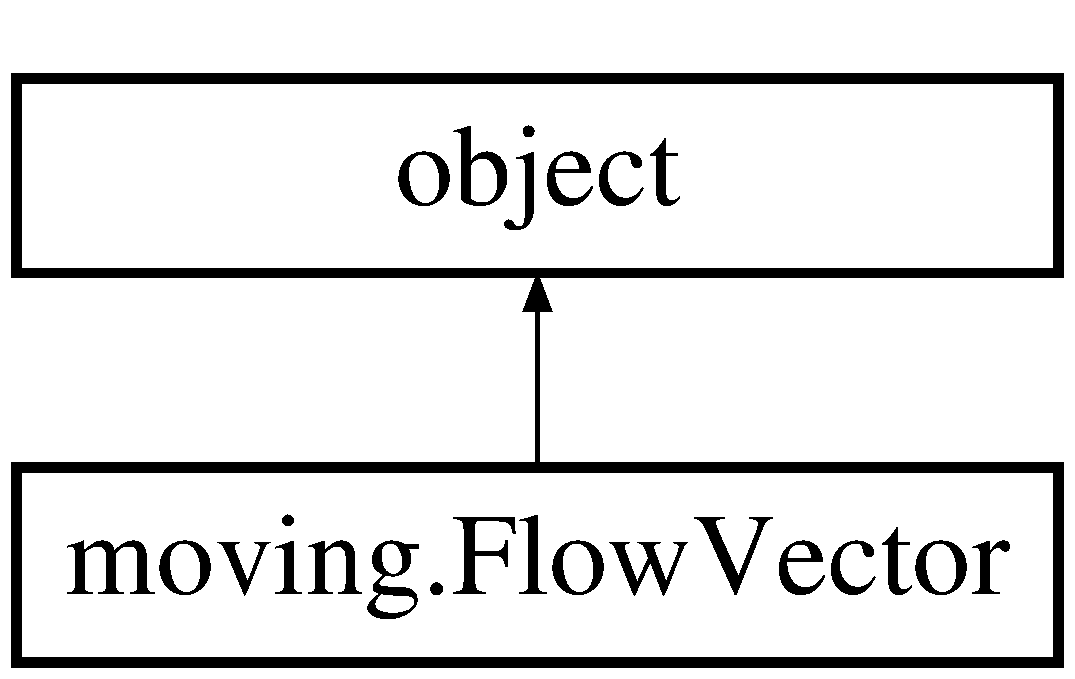
\includegraphics[height=2.000000cm]{classmoving_1_1FlowVector}
\end{center}
\end{figure}
\subsubsection*{Public Member Functions}
\begin{DoxyCompactItemize}
\item 
def \hyperlink{classmoving_1_1FlowVector_ab002fb0e01fd32d939cf6d9ecca12aaa}{\-\_\-\-\_\-init\-\_\-\-\_\-}
\item 
def \hyperlink{classmoving_1_1FlowVector_affd5d19b9c1df9240ec735d2bcf8c354}{\-\_\-\-\_\-add\-\_\-\-\_\-}
\item 
def \hyperlink{classmoving_1_1FlowVector_aec4763f51be2170c567c9d672ea12fb6}{multiply}
\item 
def \hyperlink{classmoving_1_1FlowVector_aa546a09abbbc265ed0ca43851c8e3ab7}{plot}
\end{DoxyCompactItemize}
\subsubsection*{Static Public Member Functions}
\begin{DoxyCompactItemize}
\item 
def \hyperlink{classmoving_1_1FlowVector_af8e4e987cb66de6ee60fb05a9a6dda4a}{similar}
\end{DoxyCompactItemize}
\subsubsection*{Public Attributes}
\begin{DoxyCompactItemize}
\item 
\hyperlink{classmoving_1_1FlowVector_a79d88d430e5b2e1d6aede942fa770348}{position}
\item 
\hyperlink{classmoving_1_1FlowVector_a91a16e07333e7e972c432d36324f2bce}{velocity}
\end{DoxyCompactItemize}


\subsubsection{Detailed Description}
\begin{DoxyVerb}Class to represent 4-D flow vectors,
ie a position and a velocity\end{DoxyVerb}
 

\subsubsection{Constructor \& Destructor Documentation}
\hypertarget{classmoving_1_1FlowVector_ab002fb0e01fd32d939cf6d9ecca12aaa}{\index{moving\-::\-Flow\-Vector@{moving\-::\-Flow\-Vector}!\-\_\-\-\_\-init\-\_\-\-\_\-@{\-\_\-\-\_\-init\-\_\-\-\_\-}}
\index{\-\_\-\-\_\-init\-\_\-\-\_\-@{\-\_\-\-\_\-init\-\_\-\-\_\-}!moving::FlowVector@{moving\-::\-Flow\-Vector}}
\paragraph[{\-\_\-\-\_\-init\-\_\-\-\_\-}]{\setlength{\rightskip}{0pt plus 5cm}def moving.\-Flow\-Vector.\-\_\-\-\_\-init\-\_\-\-\_\- (
\begin{DoxyParamCaption}
\item[{}]{self, }
\item[{}]{position, }
\item[{}]{velocity}
\end{DoxyParamCaption}
)}}\label{classmoving_1_1FlowVector_ab002fb0e01fd32d939cf6d9ecca12aaa}


\subsubsection{Member Function Documentation}
\hypertarget{classmoving_1_1FlowVector_affd5d19b9c1df9240ec735d2bcf8c354}{\index{moving\-::\-Flow\-Vector@{moving\-::\-Flow\-Vector}!\-\_\-\-\_\-add\-\_\-\-\_\-@{\-\_\-\-\_\-add\-\_\-\-\_\-}}
\index{\-\_\-\-\_\-add\-\_\-\-\_\-@{\-\_\-\-\_\-add\-\_\-\-\_\-}!moving::FlowVector@{moving\-::\-Flow\-Vector}}
\paragraph[{\-\_\-\-\_\-add\-\_\-\-\_\-}]{\setlength{\rightskip}{0pt plus 5cm}def moving.\-Flow\-Vector.\-\_\-\-\_\-add\-\_\-\-\_\- (
\begin{DoxyParamCaption}
\item[{}]{self, }
\item[{}]{other}
\end{DoxyParamCaption}
)}}\label{classmoving_1_1FlowVector_affd5d19b9c1df9240ec735d2bcf8c354}


References moving.\-Flow\-Vector.\-position, and moving.\-Flow\-Vector.\-velocity.

\hypertarget{classmoving_1_1FlowVector_aec4763f51be2170c567c9d672ea12fb6}{\index{moving\-::\-Flow\-Vector@{moving\-::\-Flow\-Vector}!multiply@{multiply}}
\index{multiply@{multiply}!moving::FlowVector@{moving\-::\-Flow\-Vector}}
\paragraph[{multiply}]{\setlength{\rightskip}{0pt plus 5cm}def moving.\-Flow\-Vector.\-multiply (
\begin{DoxyParamCaption}
\item[{}]{self, }
\item[{}]{alpha}
\end{DoxyParamCaption}
)}}\label{classmoving_1_1FlowVector_aec4763f51be2170c567c9d672ea12fb6}
\hypertarget{classmoving_1_1FlowVector_aa546a09abbbc265ed0ca43851c8e3ab7}{\index{moving\-::\-Flow\-Vector@{moving\-::\-Flow\-Vector}!plot@{plot}}
\index{plot@{plot}!moving::FlowVector@{moving\-::\-Flow\-Vector}}
\paragraph[{plot}]{\setlength{\rightskip}{0pt plus 5cm}def moving.\-Flow\-Vector.\-plot (
\begin{DoxyParamCaption}
\item[{}]{self, }
\item[{}]{options = {\ttfamily ''}, }
\item[{}]{kwargs}
\end{DoxyParamCaption}
)}}\label{classmoving_1_1FlowVector_aa546a09abbbc265ed0ca43851c8e3ab7}
\hypertarget{classmoving_1_1FlowVector_af8e4e987cb66de6ee60fb05a9a6dda4a}{\index{moving\-::\-Flow\-Vector@{moving\-::\-Flow\-Vector}!similar@{similar}}
\index{similar@{similar}!moving::FlowVector@{moving\-::\-Flow\-Vector}}
\paragraph[{similar}]{\setlength{\rightskip}{0pt plus 5cm}def moving.\-Flow\-Vector.\-similar (
\begin{DoxyParamCaption}
\item[{}]{f1, }
\item[{}]{f2, }
\item[{}]{max\-Distance2, }
\item[{}]{max\-Deltavelocity2}
\end{DoxyParamCaption}
)\hspace{0.3cm}{\ttfamily [static]}}}\label{classmoving_1_1FlowVector_af8e4e987cb66de6ee60fb05a9a6dda4a}


\subsubsection{Member Data Documentation}
\hypertarget{classmoving_1_1FlowVector_a79d88d430e5b2e1d6aede942fa770348}{\index{moving\-::\-Flow\-Vector@{moving\-::\-Flow\-Vector}!position@{position}}
\index{position@{position}!moving::FlowVector@{moving\-::\-Flow\-Vector}}
\paragraph[{position}]{\setlength{\rightskip}{0pt plus 5cm}moving.\-Flow\-Vector.\-position}}\label{classmoving_1_1FlowVector_a79d88d430e5b2e1d6aede942fa770348}
\hypertarget{classmoving_1_1FlowVector_a91a16e07333e7e972c432d36324f2bce}{\index{moving\-::\-Flow\-Vector@{moving\-::\-Flow\-Vector}!velocity@{velocity}}
\index{velocity@{velocity}!moving::FlowVector@{moving\-::\-Flow\-Vector}}
\paragraph[{velocity}]{\setlength{\rightskip}{0pt plus 5cm}moving.\-Flow\-Vector.\-velocity}}\label{classmoving_1_1FlowVector_a91a16e07333e7e972c432d36324f2bce}


The documentation for this class was generated from the following file\-:\begin{DoxyCompactItemize}
\item 
python/\hyperlink{moving_8py}{moving.\-py}\end{DoxyCompactItemize}

\hypertarget{classtraffic__engineering_1_1FourWayIntersection}{\subsection{traffic\-\_\-engineering.\-Four\-Way\-Intersection Class Reference}
\label{classtraffic__engineering_1_1FourWayIntersection}\index{traffic\-\_\-engineering.\-Four\-Way\-Intersection@{traffic\-\_\-engineering.\-Four\-Way\-Intersection}}
}
Inheritance diagram for traffic\-\_\-engineering.\-Four\-Way\-Intersection\-:\begin{figure}[H]
\begin{center}
\leavevmode
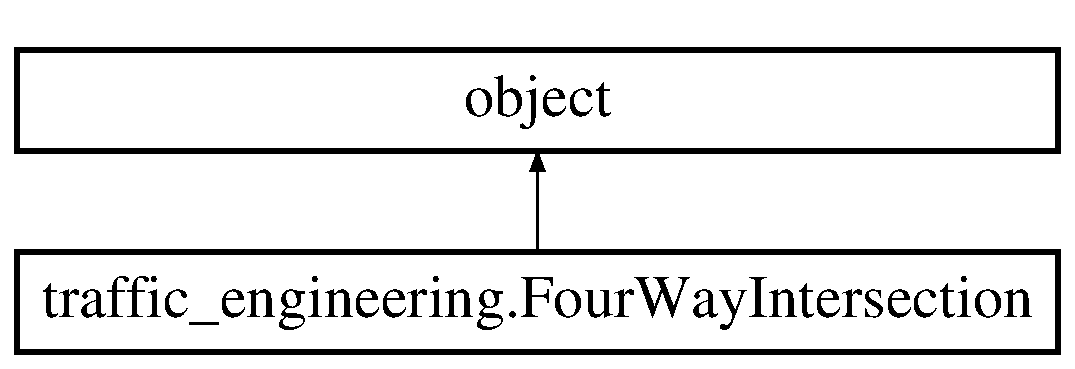
\includegraphics[height=2.000000cm]{classtraffic__engineering_1_1FourWayIntersection}
\end{center}
\end{figure}
\subsubsection*{Public Member Functions}
\begin{DoxyCompactItemize}
\item 
def \hyperlink{classtraffic__engineering_1_1FourWayIntersection_a689d2552e3b11345f7df40ecb82f3ffc}{\-\_\-\-\_\-init\-\_\-\-\_\-}
\item 
def \hyperlink{classtraffic__engineering_1_1FourWayIntersection_a7b83cbcc08c0e8ce00fe9db7efac988f}{plot}
\end{DoxyCompactItemize}
\subsubsection*{Public Attributes}
\begin{DoxyCompactItemize}
\item 
\hyperlink{classtraffic__engineering_1_1FourWayIntersection_a1eda03581ffad141eca9e1cea631ba6f}{dimension}
\item 
\hyperlink{classtraffic__engineering_1_1FourWayIntersection_a787284cf8c1dfa72c3ca408c0b467d9c}{coord\-X}
\item 
\hyperlink{classtraffic__engineering_1_1FourWayIntersection_a0b85dbf962f6d0ed264c33826be93888}{coord\-Y}
\end{DoxyCompactItemize}


\subsubsection{Detailed Description}
\begin{DoxyVerb}Simple class for simple intersection outline\end{DoxyVerb}
 

\subsubsection{Constructor \& Destructor Documentation}
\hypertarget{classtraffic__engineering_1_1FourWayIntersection_a689d2552e3b11345f7df40ecb82f3ffc}{\index{traffic\-\_\-engineering\-::\-Four\-Way\-Intersection@{traffic\-\_\-engineering\-::\-Four\-Way\-Intersection}!\-\_\-\-\_\-init\-\_\-\-\_\-@{\-\_\-\-\_\-init\-\_\-\-\_\-}}
\index{\-\_\-\-\_\-init\-\_\-\-\_\-@{\-\_\-\-\_\-init\-\_\-\-\_\-}!traffic_engineering::FourWayIntersection@{traffic\-\_\-engineering\-::\-Four\-Way\-Intersection}}
\paragraph[{\-\_\-\-\_\-init\-\_\-\-\_\-}]{\setlength{\rightskip}{0pt plus 5cm}def traffic\-\_\-engineering.\-Four\-Way\-Intersection.\-\_\-\-\_\-init\-\_\-\-\_\- (
\begin{DoxyParamCaption}
\item[{}]{self, }
\item[{}]{dimension, }
\item[{}]{coord\-X, }
\item[{}]{coord\-Y}
\end{DoxyParamCaption}
)}}\label{classtraffic__engineering_1_1FourWayIntersection_a689d2552e3b11345f7df40ecb82f3ffc}


\subsubsection{Member Function Documentation}
\hypertarget{classtraffic__engineering_1_1FourWayIntersection_a7b83cbcc08c0e8ce00fe9db7efac988f}{\index{traffic\-\_\-engineering\-::\-Four\-Way\-Intersection@{traffic\-\_\-engineering\-::\-Four\-Way\-Intersection}!plot@{plot}}
\index{plot@{plot}!traffic_engineering::FourWayIntersection@{traffic\-\_\-engineering\-::\-Four\-Way\-Intersection}}
\paragraph[{plot}]{\setlength{\rightskip}{0pt plus 5cm}def traffic\-\_\-engineering.\-Four\-Way\-Intersection.\-plot (
\begin{DoxyParamCaption}
\item[{}]{self, }
\item[{}]{options = {\ttfamily 'k'}}
\end{DoxyParamCaption}
)}}\label{classtraffic__engineering_1_1FourWayIntersection_a7b83cbcc08c0e8ce00fe9db7efac988f}


References traffic\-\_\-engineering.\-Four\-Way\-Intersection.\-coord\-X, traffic\-\_\-engineering.\-Four\-Way\-Intersection.\-coord\-Y, and traffic\-\_\-engineering.\-Four\-Way\-Intersection.\-dimension.



\subsubsection{Member Data Documentation}
\hypertarget{classtraffic__engineering_1_1FourWayIntersection_a787284cf8c1dfa72c3ca408c0b467d9c}{\index{traffic\-\_\-engineering\-::\-Four\-Way\-Intersection@{traffic\-\_\-engineering\-::\-Four\-Way\-Intersection}!coord\-X@{coord\-X}}
\index{coord\-X@{coord\-X}!traffic_engineering::FourWayIntersection@{traffic\-\_\-engineering\-::\-Four\-Way\-Intersection}}
\paragraph[{coord\-X}]{\setlength{\rightskip}{0pt plus 5cm}traffic\-\_\-engineering.\-Four\-Way\-Intersection.\-coord\-X}}\label{classtraffic__engineering_1_1FourWayIntersection_a787284cf8c1dfa72c3ca408c0b467d9c}
\hypertarget{classtraffic__engineering_1_1FourWayIntersection_a0b85dbf962f6d0ed264c33826be93888}{\index{traffic\-\_\-engineering\-::\-Four\-Way\-Intersection@{traffic\-\_\-engineering\-::\-Four\-Way\-Intersection}!coord\-Y@{coord\-Y}}
\index{coord\-Y@{coord\-Y}!traffic_engineering::FourWayIntersection@{traffic\-\_\-engineering\-::\-Four\-Way\-Intersection}}
\paragraph[{coord\-Y}]{\setlength{\rightskip}{0pt plus 5cm}traffic\-\_\-engineering.\-Four\-Way\-Intersection.\-coord\-Y}}\label{classtraffic__engineering_1_1FourWayIntersection_a0b85dbf962f6d0ed264c33826be93888}
\hypertarget{classtraffic__engineering_1_1FourWayIntersection_a1eda03581ffad141eca9e1cea631ba6f}{\index{traffic\-\_\-engineering\-::\-Four\-Way\-Intersection@{traffic\-\_\-engineering\-::\-Four\-Way\-Intersection}!dimension@{dimension}}
\index{dimension@{dimension}!traffic_engineering::FourWayIntersection@{traffic\-\_\-engineering\-::\-Four\-Way\-Intersection}}
\paragraph[{dimension}]{\setlength{\rightskip}{0pt plus 5cm}traffic\-\_\-engineering.\-Four\-Way\-Intersection.\-dimension}}\label{classtraffic__engineering_1_1FourWayIntersection_a1eda03581ffad141eca9e1cea631ba6f}


The documentation for this class was generated from the following file\-:\begin{DoxyCompactItemize}
\item 
python/\hyperlink{traffic__engineering_8py}{traffic\-\_\-engineering.\-py}\end{DoxyCompactItemize}

\hypertarget{classtraffic__engineering_1_1FundamentalDiagram}{\subsection{traffic\-\_\-engineering.\-Fundamental\-Diagram Class Reference}
\label{classtraffic__engineering_1_1FundamentalDiagram}\index{traffic\-\_\-engineering.\-Fundamental\-Diagram@{traffic\-\_\-engineering.\-Fundamental\-Diagram}}
}
Inheritance diagram for traffic\-\_\-engineering.\-Fundamental\-Diagram\-:\begin{figure}[H]
\begin{center}
\leavevmode
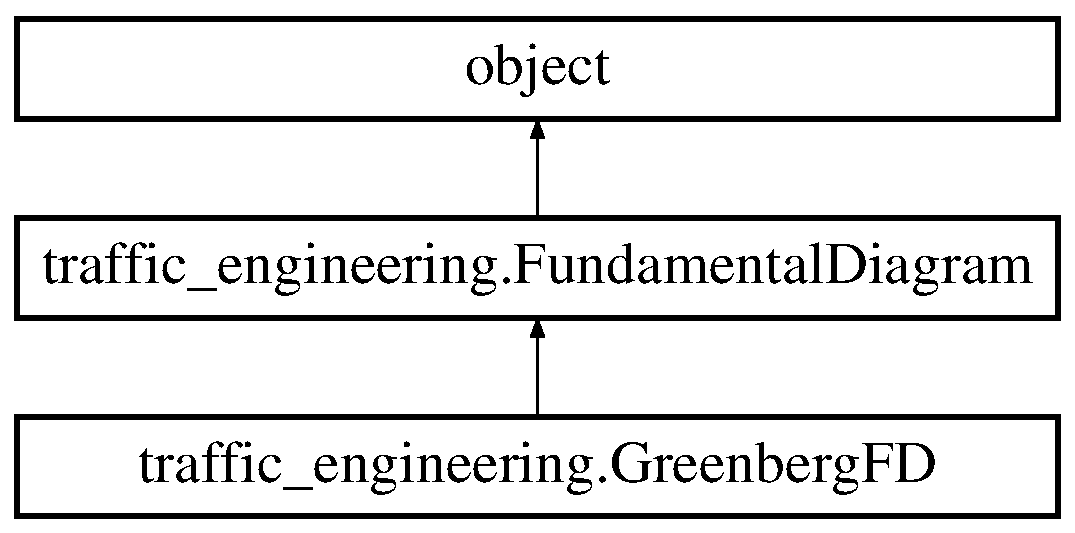
\includegraphics[height=3.000000cm]{classtraffic__engineering_1_1FundamentalDiagram}
\end{center}
\end{figure}
\subsubsection*{Public Member Functions}
\begin{DoxyCompactItemize}
\item 
def \hyperlink{classtraffic__engineering_1_1FundamentalDiagram_ac169210ecd9fc3bdc667c5a3e537c33c}{\-\_\-\-\_\-init\-\_\-\-\_\-}
\item 
def \hyperlink{classtraffic__engineering_1_1FundamentalDiagram_a4164af14787ea9a33e14fa7951dd0a89}{q}
\item 
def \hyperlink{classtraffic__engineering_1_1FundamentalDiagram_a9aeca0e6b4838b1a39fbf7676f542af3}{plot\-V\-K}
\item 
def \hyperlink{classtraffic__engineering_1_1FundamentalDiagram_a3344d9b165822c29320ee42397cf1c7e}{plot\-Q\-K}
\end{DoxyCompactItemize}
\subsubsection*{Static Public Member Functions}
\begin{DoxyCompactItemize}
\item 
def \hyperlink{classtraffic__engineering_1_1FundamentalDiagram_a0e878df5457a0d35c6386b960e0ad618}{mean\-Headway}
\item 
def \hyperlink{classtraffic__engineering_1_1FundamentalDiagram_ae211a3b47f9d7243ce1db13cd112720f}{mean\-Spacing}
\end{DoxyCompactItemize}
\subsubsection*{Public Attributes}
\begin{DoxyCompactItemize}
\item 
\hyperlink{classtraffic__engineering_1_1FundamentalDiagram_a83c90c78828bc2fb7b608e97e29b436c}{name}
\end{DoxyCompactItemize}


\subsubsection{Detailed Description}
\begin{DoxyVerb}\end{DoxyVerb}
 

\subsubsection{Constructor \& Destructor Documentation}
\hypertarget{classtraffic__engineering_1_1FundamentalDiagram_ac169210ecd9fc3bdc667c5a3e537c33c}{\index{traffic\-\_\-engineering\-::\-Fundamental\-Diagram@{traffic\-\_\-engineering\-::\-Fundamental\-Diagram}!\-\_\-\-\_\-init\-\_\-\-\_\-@{\-\_\-\-\_\-init\-\_\-\-\_\-}}
\index{\-\_\-\-\_\-init\-\_\-\-\_\-@{\-\_\-\-\_\-init\-\_\-\-\_\-}!traffic_engineering::FundamentalDiagram@{traffic\-\_\-engineering\-::\-Fundamental\-Diagram}}
\paragraph[{\-\_\-\-\_\-init\-\_\-\-\_\-}]{\setlength{\rightskip}{0pt plus 5cm}def traffic\-\_\-engineering.\-Fundamental\-Diagram.\-\_\-\-\_\-init\-\_\-\-\_\- (
\begin{DoxyParamCaption}
\item[{}]{self, }
\item[{}]{name}
\end{DoxyParamCaption}
)}}\label{classtraffic__engineering_1_1FundamentalDiagram_ac169210ecd9fc3bdc667c5a3e537c33c}


\subsubsection{Member Function Documentation}
\hypertarget{classtraffic__engineering_1_1FundamentalDiagram_a0e878df5457a0d35c6386b960e0ad618}{\index{traffic\-\_\-engineering\-::\-Fundamental\-Diagram@{traffic\-\_\-engineering\-::\-Fundamental\-Diagram}!mean\-Headway@{mean\-Headway}}
\index{mean\-Headway@{mean\-Headway}!traffic_engineering::FundamentalDiagram@{traffic\-\_\-engineering\-::\-Fundamental\-Diagram}}
\paragraph[{mean\-Headway}]{\setlength{\rightskip}{0pt plus 5cm}def traffic\-\_\-engineering.\-Fundamental\-Diagram.\-mean\-Headway (
\begin{DoxyParamCaption}
\item[{}]{k}
\end{DoxyParamCaption}
)\hspace{0.3cm}{\ttfamily [static]}}}\label{classtraffic__engineering_1_1FundamentalDiagram_a0e878df5457a0d35c6386b960e0ad618}
\hypertarget{classtraffic__engineering_1_1FundamentalDiagram_ae211a3b47f9d7243ce1db13cd112720f}{\index{traffic\-\_\-engineering\-::\-Fundamental\-Diagram@{traffic\-\_\-engineering\-::\-Fundamental\-Diagram}!mean\-Spacing@{mean\-Spacing}}
\index{mean\-Spacing@{mean\-Spacing}!traffic_engineering::FundamentalDiagram@{traffic\-\_\-engineering\-::\-Fundamental\-Diagram}}
\paragraph[{mean\-Spacing}]{\setlength{\rightskip}{0pt plus 5cm}def traffic\-\_\-engineering.\-Fundamental\-Diagram.\-mean\-Spacing (
\begin{DoxyParamCaption}
\item[{}]{q}
\end{DoxyParamCaption}
)\hspace{0.3cm}{\ttfamily [static]}}}\label{classtraffic__engineering_1_1FundamentalDiagram_ae211a3b47f9d7243ce1db13cd112720f}
\hypertarget{classtraffic__engineering_1_1FundamentalDiagram_a3344d9b165822c29320ee42397cf1c7e}{\index{traffic\-\_\-engineering\-::\-Fundamental\-Diagram@{traffic\-\_\-engineering\-::\-Fundamental\-Diagram}!plot\-Q\-K@{plot\-Q\-K}}
\index{plot\-Q\-K@{plot\-Q\-K}!traffic_engineering::FundamentalDiagram@{traffic\-\_\-engineering\-::\-Fundamental\-Diagram}}
\paragraph[{plot\-Q\-K}]{\setlength{\rightskip}{0pt plus 5cm}def traffic\-\_\-engineering.\-Fundamental\-Diagram.\-plot\-Q\-K (
\begin{DoxyParamCaption}
\item[{}]{self, }
\item[{}]{language = {\ttfamily 'fr'}, }
\item[{}]{units = {\ttfamily \{\}}}
\end{DoxyParamCaption}
)}}\label{classtraffic__engineering_1_1FundamentalDiagram_a3344d9b165822c29320ee42397cf1c7e}


References traffic\-\_\-engineering.\-Greenberg\-F\-D.\-kj, and traffic\-\_\-engineering.\-Fundamental\-Diagram.\-q().

\hypertarget{classtraffic__engineering_1_1FundamentalDiagram_a9aeca0e6b4838b1a39fbf7676f542af3}{\index{traffic\-\_\-engineering\-::\-Fundamental\-Diagram@{traffic\-\_\-engineering\-::\-Fundamental\-Diagram}!plot\-V\-K@{plot\-V\-K}}
\index{plot\-V\-K@{plot\-V\-K}!traffic_engineering::FundamentalDiagram@{traffic\-\_\-engineering\-::\-Fundamental\-Diagram}}
\paragraph[{plot\-V\-K}]{\setlength{\rightskip}{0pt plus 5cm}def traffic\-\_\-engineering.\-Fundamental\-Diagram.\-plot\-V\-K (
\begin{DoxyParamCaption}
\item[{}]{self, }
\item[{}]{language = {\ttfamily 'fr'}, }
\item[{}]{units = {\ttfamily \{\}}}
\end{DoxyParamCaption}
)}}\label{classtraffic__engineering_1_1FundamentalDiagram_a9aeca0e6b4838b1a39fbf7676f542af3}


References traffic\-\_\-engineering.\-Greenberg\-F\-D.\-kj, and traffic\-\_\-engineering.\-Greenberg\-F\-D.\-v().

\hypertarget{classtraffic__engineering_1_1FundamentalDiagram_a4164af14787ea9a33e14fa7951dd0a89}{\index{traffic\-\_\-engineering\-::\-Fundamental\-Diagram@{traffic\-\_\-engineering\-::\-Fundamental\-Diagram}!q@{q}}
\index{q@{q}!traffic_engineering::FundamentalDiagram@{traffic\-\_\-engineering\-::\-Fundamental\-Diagram}}
\paragraph[{q}]{\setlength{\rightskip}{0pt plus 5cm}def traffic\-\_\-engineering.\-Fundamental\-Diagram.\-q (
\begin{DoxyParamCaption}
\item[{}]{self, }
\item[{}]{k}
\end{DoxyParamCaption}
)}}\label{classtraffic__engineering_1_1FundamentalDiagram_a4164af14787ea9a33e14fa7951dd0a89}


References traffic\-\_\-engineering.\-Greenberg\-F\-D.\-v().



\subsubsection{Member Data Documentation}
\hypertarget{classtraffic__engineering_1_1FundamentalDiagram_a83c90c78828bc2fb7b608e97e29b436c}{\index{traffic\-\_\-engineering\-::\-Fundamental\-Diagram@{traffic\-\_\-engineering\-::\-Fundamental\-Diagram}!name@{name}}
\index{name@{name}!traffic_engineering::FundamentalDiagram@{traffic\-\_\-engineering\-::\-Fundamental\-Diagram}}
\paragraph[{name}]{\setlength{\rightskip}{0pt plus 5cm}traffic\-\_\-engineering.\-Fundamental\-Diagram.\-name}}\label{classtraffic__engineering_1_1FundamentalDiagram_a83c90c78828bc2fb7b608e97e29b436c}


The documentation for this class was generated from the following file\-:\begin{DoxyCompactItemize}
\item 
python/\hyperlink{traffic__engineering_8py}{traffic\-\_\-engineering.\-py}\end{DoxyCompactItemize}

\hypertarget{classtraffic__engineering_1_1GreenbergFD}{\subsection{traffic\-\_\-engineering.\-Greenberg\-F\-D Class Reference}
\label{classtraffic__engineering_1_1GreenbergFD}\index{traffic\-\_\-engineering.\-Greenberg\-F\-D@{traffic\-\_\-engineering.\-Greenberg\-F\-D}}
}
Inheritance diagram for traffic\-\_\-engineering.\-Greenberg\-F\-D\-:\begin{figure}[H]
\begin{center}
\leavevmode
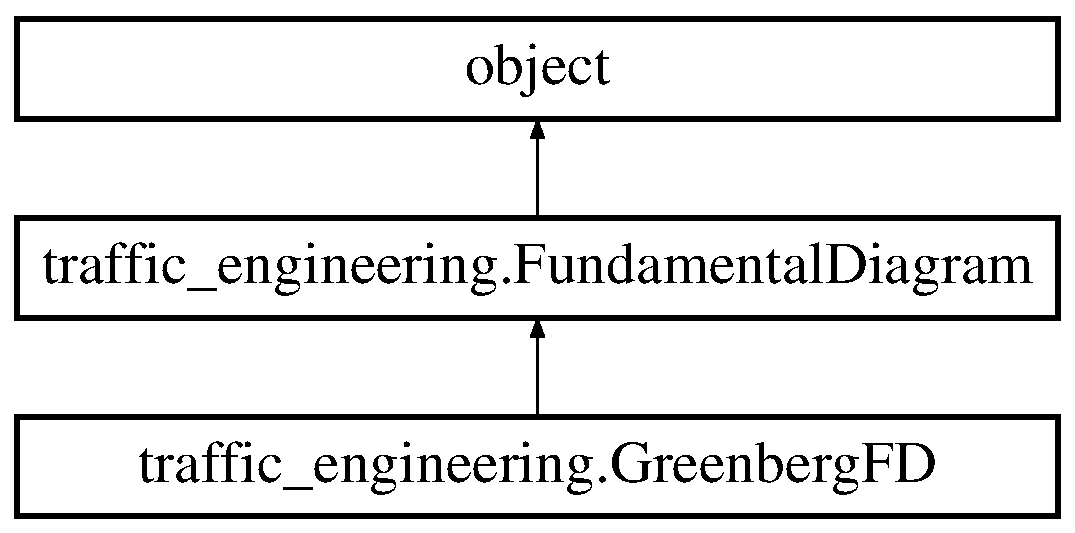
\includegraphics[height=3.000000cm]{classtraffic__engineering_1_1GreenbergFD}
\end{center}
\end{figure}
\subsubsection*{Public Member Functions}
\begin{DoxyCompactItemize}
\item 
def \hyperlink{classtraffic__engineering_1_1GreenbergFD_a514f0f2687de708e1badc7ec11a1a1ec}{\-\_\-\-\_\-init\-\_\-\-\_\-}
\item 
def \hyperlink{classtraffic__engineering_1_1GreenbergFD_aa63b3b26baa44f1ee5d6a8dc84b8baa3}{v}
\item 
def \hyperlink{classtraffic__engineering_1_1GreenbergFD_a23fb323e718ad56acae0f174a465c90c}{critical\-Density}
\item 
def \hyperlink{classtraffic__engineering_1_1GreenbergFD_a8acd2a1a27936fb5be6ae8049cbe9711}{capacity}
\end{DoxyCompactItemize}
\subsubsection*{Public Attributes}
\begin{DoxyCompactItemize}
\item 
\hyperlink{classtraffic__engineering_1_1GreenbergFD_a7134c8a55120d951b112818fe9724285}{vc}
\item 
\hyperlink{classtraffic__engineering_1_1GreenbergFD_ac4c696e59088247b4ede81c4d89e9175}{kj}
\item 
\hyperlink{classtraffic__engineering_1_1GreenbergFD_ae1655c5902b4a0a052076c1f3cf9815f}{kc}
\item 
\hyperlink{classtraffic__engineering_1_1GreenbergFD_ae75ead70e12104991e35ac8e81c9257e}{qmax}
\end{DoxyCompactItemize}
\subsubsection*{Additional Inherited Members}


\subsubsection{Detailed Description}
\begin{DoxyVerb}Speed is the logarithm of density\end{DoxyVerb}
 

\subsubsection{Constructor \& Destructor Documentation}
\hypertarget{classtraffic__engineering_1_1GreenbergFD_a514f0f2687de708e1badc7ec11a1a1ec}{\index{traffic\-\_\-engineering\-::\-Greenberg\-F\-D@{traffic\-\_\-engineering\-::\-Greenberg\-F\-D}!\-\_\-\-\_\-init\-\_\-\-\_\-@{\-\_\-\-\_\-init\-\_\-\-\_\-}}
\index{\-\_\-\-\_\-init\-\_\-\-\_\-@{\-\_\-\-\_\-init\-\_\-\-\_\-}!traffic_engineering::GreenbergFD@{traffic\-\_\-engineering\-::\-Greenberg\-F\-D}}
\paragraph[{\-\_\-\-\_\-init\-\_\-\-\_\-}]{\setlength{\rightskip}{0pt plus 5cm}def traffic\-\_\-engineering.\-Greenberg\-F\-D.\-\_\-\-\_\-init\-\_\-\-\_\- (
\begin{DoxyParamCaption}
\item[{}]{self, }
\item[{}]{vc, }
\item[{}]{kj}
\end{DoxyParamCaption}
)}}\label{classtraffic__engineering_1_1GreenbergFD_a514f0f2687de708e1badc7ec11a1a1ec}


\subsubsection{Member Function Documentation}
\hypertarget{classtraffic__engineering_1_1GreenbergFD_a8acd2a1a27936fb5be6ae8049cbe9711}{\index{traffic\-\_\-engineering\-::\-Greenberg\-F\-D@{traffic\-\_\-engineering\-::\-Greenberg\-F\-D}!capacity@{capacity}}
\index{capacity@{capacity}!traffic_engineering::GreenbergFD@{traffic\-\_\-engineering\-::\-Greenberg\-F\-D}}
\paragraph[{capacity}]{\setlength{\rightskip}{0pt plus 5cm}def traffic\-\_\-engineering.\-Greenberg\-F\-D.\-capacity (
\begin{DoxyParamCaption}
\item[{}]{self}
\end{DoxyParamCaption}
)}}\label{classtraffic__engineering_1_1GreenbergFD_a8acd2a1a27936fb5be6ae8049cbe9711}
\hypertarget{classtraffic__engineering_1_1GreenbergFD_a23fb323e718ad56acae0f174a465c90c}{\index{traffic\-\_\-engineering\-::\-Greenberg\-F\-D@{traffic\-\_\-engineering\-::\-Greenberg\-F\-D}!critical\-Density@{critical\-Density}}
\index{critical\-Density@{critical\-Density}!traffic_engineering::GreenbergFD@{traffic\-\_\-engineering\-::\-Greenberg\-F\-D}}
\paragraph[{critical\-Density}]{\setlength{\rightskip}{0pt plus 5cm}def traffic\-\_\-engineering.\-Greenberg\-F\-D.\-critical\-Density (
\begin{DoxyParamCaption}
\item[{}]{self}
\end{DoxyParamCaption}
)}}\label{classtraffic__engineering_1_1GreenbergFD_a23fb323e718ad56acae0f174a465c90c}
\hypertarget{classtraffic__engineering_1_1GreenbergFD_aa63b3b26baa44f1ee5d6a8dc84b8baa3}{\index{traffic\-\_\-engineering\-::\-Greenberg\-F\-D@{traffic\-\_\-engineering\-::\-Greenberg\-F\-D}!v@{v}}
\index{v@{v}!traffic_engineering::GreenbergFD@{traffic\-\_\-engineering\-::\-Greenberg\-F\-D}}
\paragraph[{v}]{\setlength{\rightskip}{0pt plus 5cm}def traffic\-\_\-engineering.\-Greenberg\-F\-D.\-v (
\begin{DoxyParamCaption}
\item[{}]{self, }
\item[{}]{k}
\end{DoxyParamCaption}
)}}\label{classtraffic__engineering_1_1GreenbergFD_aa63b3b26baa44f1ee5d6a8dc84b8baa3}


References traffic\-\_\-engineering.\-Greenberg\-F\-D.\-kj, and traffic\-\_\-engineering.\-Greenberg\-F\-D.\-vc.



\subsubsection{Member Data Documentation}
\hypertarget{classtraffic__engineering_1_1GreenbergFD_ae1655c5902b4a0a052076c1f3cf9815f}{\index{traffic\-\_\-engineering\-::\-Greenberg\-F\-D@{traffic\-\_\-engineering\-::\-Greenberg\-F\-D}!kc@{kc}}
\index{kc@{kc}!traffic_engineering::GreenbergFD@{traffic\-\_\-engineering\-::\-Greenberg\-F\-D}}
\paragraph[{kc}]{\setlength{\rightskip}{0pt plus 5cm}traffic\-\_\-engineering.\-Greenberg\-F\-D.\-kc}}\label{classtraffic__engineering_1_1GreenbergFD_ae1655c5902b4a0a052076c1f3cf9815f}
\hypertarget{classtraffic__engineering_1_1GreenbergFD_ac4c696e59088247b4ede81c4d89e9175}{\index{traffic\-\_\-engineering\-::\-Greenberg\-F\-D@{traffic\-\_\-engineering\-::\-Greenberg\-F\-D}!kj@{kj}}
\index{kj@{kj}!traffic_engineering::GreenbergFD@{traffic\-\_\-engineering\-::\-Greenberg\-F\-D}}
\paragraph[{kj}]{\setlength{\rightskip}{0pt plus 5cm}traffic\-\_\-engineering.\-Greenberg\-F\-D.\-kj}}\label{classtraffic__engineering_1_1GreenbergFD_ac4c696e59088247b4ede81c4d89e9175}
\hypertarget{classtraffic__engineering_1_1GreenbergFD_ae75ead70e12104991e35ac8e81c9257e}{\index{traffic\-\_\-engineering\-::\-Greenberg\-F\-D@{traffic\-\_\-engineering\-::\-Greenberg\-F\-D}!qmax@{qmax}}
\index{qmax@{qmax}!traffic_engineering::GreenbergFD@{traffic\-\_\-engineering\-::\-Greenberg\-F\-D}}
\paragraph[{qmax}]{\setlength{\rightskip}{0pt plus 5cm}traffic\-\_\-engineering.\-Greenberg\-F\-D.\-qmax}}\label{classtraffic__engineering_1_1GreenbergFD_ae75ead70e12104991e35ac8e81c9257e}
\hypertarget{classtraffic__engineering_1_1GreenbergFD_a7134c8a55120d951b112818fe9724285}{\index{traffic\-\_\-engineering\-::\-Greenberg\-F\-D@{traffic\-\_\-engineering\-::\-Greenberg\-F\-D}!vc@{vc}}
\index{vc@{vc}!traffic_engineering::GreenbergFD@{traffic\-\_\-engineering\-::\-Greenberg\-F\-D}}
\paragraph[{vc}]{\setlength{\rightskip}{0pt plus 5cm}traffic\-\_\-engineering.\-Greenberg\-F\-D.\-vc}}\label{classtraffic__engineering_1_1GreenbergFD_a7134c8a55120d951b112818fe9724285}


The documentation for this class was generated from the following file\-:\begin{DoxyCompactItemize}
\item 
python/\hyperlink{traffic__engineering_8py}{traffic\-\_\-engineering.\-py}\end{DoxyCompactItemize}

\hypertarget{structCatch_1_1IConfig}{\subsection{Catch\-:\-:I\-Config Struct Reference}
\label{structCatch_1_1IConfig}\index{Catch\-::\-I\-Config@{Catch\-::\-I\-Config}}
}


{\ttfamily \#include $<$catch.\-hpp$>$}

\subsubsection*{Public Member Functions}
\begin{DoxyCompactItemize}
\item 
virtual \hyperlink{structCatch_1_1IConfig_adadf7c57478e4b0c83bea5b38d2dbc87}{$\sim$\-I\-Config} ()
\item 
virtual bool \hyperlink{structCatch_1_1IConfig_aadb95f849359de1e6eb915aab063e542}{allow\-Throws} () const =0
\end{DoxyCompactItemize}


\subsubsection{Constructor \& Destructor Documentation}
\hypertarget{structCatch_1_1IConfig_adadf7c57478e4b0c83bea5b38d2dbc87}{\index{Catch\-::\-I\-Config@{Catch\-::\-I\-Config}!$\sim$\-I\-Config@{$\sim$\-I\-Config}}
\index{$\sim$\-I\-Config@{$\sim$\-I\-Config}!Catch::IConfig@{Catch\-::\-I\-Config}}
\paragraph[{$\sim$\-I\-Config}]{\setlength{\rightskip}{0pt plus 5cm}virtual Catch\-::\-I\-Config\-::$\sim$\-I\-Config (
\begin{DoxyParamCaption}
{}
\end{DoxyParamCaption}
)\hspace{0.3cm}{\ttfamily [inline]}, {\ttfamily [virtual]}}}\label{structCatch_1_1IConfig_adadf7c57478e4b0c83bea5b38d2dbc87}


\subsubsection{Member Function Documentation}
\hypertarget{structCatch_1_1IConfig_aadb95f849359de1e6eb915aab063e542}{\index{Catch\-::\-I\-Config@{Catch\-::\-I\-Config}!allow\-Throws@{allow\-Throws}}
\index{allow\-Throws@{allow\-Throws}!Catch::IConfig@{Catch\-::\-I\-Config}}
\paragraph[{allow\-Throws}]{\setlength{\rightskip}{0pt plus 5cm}virtual bool Catch\-::\-I\-Config\-::allow\-Throws (
\begin{DoxyParamCaption}
{}
\end{DoxyParamCaption}
) const\hspace{0.3cm}{\ttfamily [pure virtual]}}}\label{structCatch_1_1IConfig_aadb95f849359de1e6eb915aab063e542}


The documentation for this struct was generated from the following file\-:\begin{DoxyCompactItemize}
\item 
include/\hyperlink{catch_8hpp}{catch.\-hpp}\end{DoxyCompactItemize}

\hypertarget{structCatch_1_1IContext}{\subsection{Catch\-:\-:I\-Context Struct Reference}
\label{structCatch_1_1IContext}\index{Catch\-::\-I\-Context@{Catch\-::\-I\-Context}}
}


{\ttfamily \#include $<$catch.\-hpp$>$}

Inheritance diagram for Catch\-:\-:I\-Context\-:\begin{figure}[H]
\begin{center}
\leavevmode
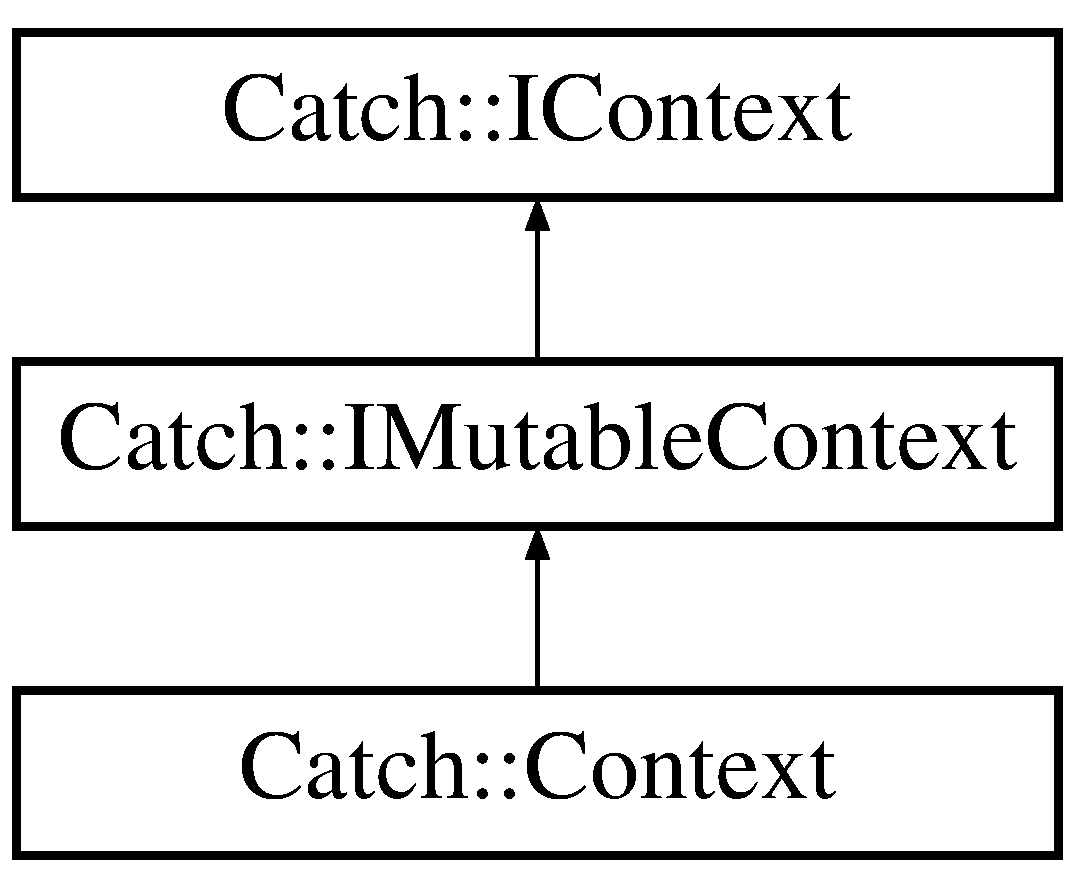
\includegraphics[height=3.000000cm]{structCatch_1_1IContext}
\end{center}
\end{figure}
\subsubsection*{Public Member Functions}
\begin{DoxyCompactItemize}
\item 
virtual \hyperlink{structCatch_1_1IContext_aeb17355c1be6c2ced5407cad7202628d}{$\sim$\-I\-Context} ()
\item 
virtual \hyperlink{structCatch_1_1IResultCapture}{I\-Result\-Capture} \& \hyperlink{structCatch_1_1IContext_a7df92cdf3d2600866bf5aeb56c236cf9}{get\-Result\-Capture} ()=0
\item 
virtual \hyperlink{structCatch_1_1IRunner}{I\-Runner} \& \hyperlink{structCatch_1_1IContext_a8106d887b354016f3d79449731b459b9}{get\-Runner} ()=0
\item 
virtual \hyperlink{structCatch_1_1IReporterRegistry}{I\-Reporter\-Registry} \& \hyperlink{structCatch_1_1IContext_a8f0076265639edd2ff42a45cc88231c3}{get\-Reporter\-Registry} ()=0
\item 
virtual \hyperlink{structCatch_1_1ITestCaseRegistry}{I\-Test\-Case\-Registry} \& \hyperlink{structCatch_1_1IContext_a2f95460e6fee34076f74c24b8c73f14a}{get\-Test\-Case\-Registry} ()=0
\item 
virtual \\*
\hyperlink{structCatch_1_1IExceptionTranslatorRegistry}{I\-Exception\-Translator\-Registry} \& \hyperlink{structCatch_1_1IContext_ae1c359211e865de05b0a717d858c5384}{get\-Exception\-Translator\-Registry} ()=0
\item 
virtual size\-\_\-t \hyperlink{structCatch_1_1IContext_a8aee59763eb426b7bfecf40bf3362583}{get\-Generator\-Index} (const std\-::string \&file\-Info, size\-\_\-t total\-Size)=0
\item 
virtual bool \hyperlink{structCatch_1_1IContext_a806f7c4ed24d51adae90418e661b24b7}{advance\-Generators\-For\-Current\-Test} ()=0
\item 
virtual const \hyperlink{structCatch_1_1IConfig}{I\-Config} $\ast$ \hyperlink{structCatch_1_1IContext_aac96dcc006c7d481eeab7163a1cf265b}{get\-Config} () const =0
\end{DoxyCompactItemize}


\subsubsection{Constructor \& Destructor Documentation}
\hypertarget{structCatch_1_1IContext_aeb17355c1be6c2ced5407cad7202628d}{\index{Catch\-::\-I\-Context@{Catch\-::\-I\-Context}!$\sim$\-I\-Context@{$\sim$\-I\-Context}}
\index{$\sim$\-I\-Context@{$\sim$\-I\-Context}!Catch::IContext@{Catch\-::\-I\-Context}}
\paragraph[{$\sim$\-I\-Context}]{\setlength{\rightskip}{0pt plus 5cm}virtual Catch\-::\-I\-Context\-::$\sim$\-I\-Context (
\begin{DoxyParamCaption}
{}
\end{DoxyParamCaption}
)\hspace{0.3cm}{\ttfamily [inline]}, {\ttfamily [virtual]}}}\label{structCatch_1_1IContext_aeb17355c1be6c2ced5407cad7202628d}


\subsubsection{Member Function Documentation}
\hypertarget{structCatch_1_1IContext_a806f7c4ed24d51adae90418e661b24b7}{\index{Catch\-::\-I\-Context@{Catch\-::\-I\-Context}!advance\-Generators\-For\-Current\-Test@{advance\-Generators\-For\-Current\-Test}}
\index{advance\-Generators\-For\-Current\-Test@{advance\-Generators\-For\-Current\-Test}!Catch::IContext@{Catch\-::\-I\-Context}}
\paragraph[{advance\-Generators\-For\-Current\-Test}]{\setlength{\rightskip}{0pt plus 5cm}virtual bool Catch\-::\-I\-Context\-::advance\-Generators\-For\-Current\-Test (
\begin{DoxyParamCaption}
{}
\end{DoxyParamCaption}
)\hspace{0.3cm}{\ttfamily [pure virtual]}}}\label{structCatch_1_1IContext_a806f7c4ed24d51adae90418e661b24b7}


Implemented in \hyperlink{classCatch_1_1Context_aa4c8d900c7168191636bf54ae5c1d501}{Catch\-::\-Context}.

\hypertarget{structCatch_1_1IContext_aac96dcc006c7d481eeab7163a1cf265b}{\index{Catch\-::\-I\-Context@{Catch\-::\-I\-Context}!get\-Config@{get\-Config}}
\index{get\-Config@{get\-Config}!Catch::IContext@{Catch\-::\-I\-Context}}
\paragraph[{get\-Config}]{\setlength{\rightskip}{0pt plus 5cm}virtual const {\bf I\-Config}$\ast$ Catch\-::\-I\-Context\-::get\-Config (
\begin{DoxyParamCaption}
{}
\end{DoxyParamCaption}
) const\hspace{0.3cm}{\ttfamily [pure virtual]}}}\label{structCatch_1_1IContext_aac96dcc006c7d481eeab7163a1cf265b}


Implemented in \hyperlink{classCatch_1_1Context_a352ac7605c53582bf278105396ce8f74}{Catch\-::\-Context}.

\hypertarget{structCatch_1_1IContext_ae1c359211e865de05b0a717d858c5384}{\index{Catch\-::\-I\-Context@{Catch\-::\-I\-Context}!get\-Exception\-Translator\-Registry@{get\-Exception\-Translator\-Registry}}
\index{get\-Exception\-Translator\-Registry@{get\-Exception\-Translator\-Registry}!Catch::IContext@{Catch\-::\-I\-Context}}
\paragraph[{get\-Exception\-Translator\-Registry}]{\setlength{\rightskip}{0pt plus 5cm}virtual {\bf I\-Exception\-Translator\-Registry}\& Catch\-::\-I\-Context\-::get\-Exception\-Translator\-Registry (
\begin{DoxyParamCaption}
{}
\end{DoxyParamCaption}
)\hspace{0.3cm}{\ttfamily [pure virtual]}}}\label{structCatch_1_1IContext_ae1c359211e865de05b0a717d858c5384}


Implemented in \hyperlink{classCatch_1_1Context_a8e3ce31c44d5b3c706a878dcdd77d7e9}{Catch\-::\-Context}.

\hypertarget{structCatch_1_1IContext_a8aee59763eb426b7bfecf40bf3362583}{\index{Catch\-::\-I\-Context@{Catch\-::\-I\-Context}!get\-Generator\-Index@{get\-Generator\-Index}}
\index{get\-Generator\-Index@{get\-Generator\-Index}!Catch::IContext@{Catch\-::\-I\-Context}}
\paragraph[{get\-Generator\-Index}]{\setlength{\rightskip}{0pt plus 5cm}virtual size\-\_\-t Catch\-::\-I\-Context\-::get\-Generator\-Index (
\begin{DoxyParamCaption}
\item[{const std\-::string \&}]{file\-Info, }
\item[{size\-\_\-t}]{total\-Size}
\end{DoxyParamCaption}
)\hspace{0.3cm}{\ttfamily [pure virtual]}}}\label{structCatch_1_1IContext_a8aee59763eb426b7bfecf40bf3362583}


Implemented in \hyperlink{classCatch_1_1Context_a06474443026c33532fdfb2ea1848eb31}{Catch\-::\-Context}.

\hypertarget{structCatch_1_1IContext_a8f0076265639edd2ff42a45cc88231c3}{\index{Catch\-::\-I\-Context@{Catch\-::\-I\-Context}!get\-Reporter\-Registry@{get\-Reporter\-Registry}}
\index{get\-Reporter\-Registry@{get\-Reporter\-Registry}!Catch::IContext@{Catch\-::\-I\-Context}}
\paragraph[{get\-Reporter\-Registry}]{\setlength{\rightskip}{0pt plus 5cm}virtual {\bf I\-Reporter\-Registry}\& Catch\-::\-I\-Context\-::get\-Reporter\-Registry (
\begin{DoxyParamCaption}
{}
\end{DoxyParamCaption}
)\hspace{0.3cm}{\ttfamily [pure virtual]}}}\label{structCatch_1_1IContext_a8f0076265639edd2ff42a45cc88231c3}


Implemented in \hyperlink{classCatch_1_1Context_aad092bba66a990c412eb5137e8a8d1fd}{Catch\-::\-Context}.

\hypertarget{structCatch_1_1IContext_a7df92cdf3d2600866bf5aeb56c236cf9}{\index{Catch\-::\-I\-Context@{Catch\-::\-I\-Context}!get\-Result\-Capture@{get\-Result\-Capture}}
\index{get\-Result\-Capture@{get\-Result\-Capture}!Catch::IContext@{Catch\-::\-I\-Context}}
\paragraph[{get\-Result\-Capture}]{\setlength{\rightskip}{0pt plus 5cm}virtual {\bf I\-Result\-Capture}\& Catch\-::\-I\-Context\-::get\-Result\-Capture (
\begin{DoxyParamCaption}
{}
\end{DoxyParamCaption}
)\hspace{0.3cm}{\ttfamily [pure virtual]}}}\label{structCatch_1_1IContext_a7df92cdf3d2600866bf5aeb56c236cf9}


Implemented in \hyperlink{classCatch_1_1Context_ae28e8862c120382a5747ffc36611271b}{Catch\-::\-Context}.

\hypertarget{structCatch_1_1IContext_a8106d887b354016f3d79449731b459b9}{\index{Catch\-::\-I\-Context@{Catch\-::\-I\-Context}!get\-Runner@{get\-Runner}}
\index{get\-Runner@{get\-Runner}!Catch::IContext@{Catch\-::\-I\-Context}}
\paragraph[{get\-Runner}]{\setlength{\rightskip}{0pt plus 5cm}virtual {\bf I\-Runner}\& Catch\-::\-I\-Context\-::get\-Runner (
\begin{DoxyParamCaption}
{}
\end{DoxyParamCaption}
)\hspace{0.3cm}{\ttfamily [pure virtual]}}}\label{structCatch_1_1IContext_a8106d887b354016f3d79449731b459b9}


Implemented in \hyperlink{classCatch_1_1Context_aa28c1fa65249a6b344d8574c3f345525}{Catch\-::\-Context}.

\hypertarget{structCatch_1_1IContext_a2f95460e6fee34076f74c24b8c73f14a}{\index{Catch\-::\-I\-Context@{Catch\-::\-I\-Context}!get\-Test\-Case\-Registry@{get\-Test\-Case\-Registry}}
\index{get\-Test\-Case\-Registry@{get\-Test\-Case\-Registry}!Catch::IContext@{Catch\-::\-I\-Context}}
\paragraph[{get\-Test\-Case\-Registry}]{\setlength{\rightskip}{0pt plus 5cm}virtual {\bf I\-Test\-Case\-Registry}\& Catch\-::\-I\-Context\-::get\-Test\-Case\-Registry (
\begin{DoxyParamCaption}
{}
\end{DoxyParamCaption}
)\hspace{0.3cm}{\ttfamily [pure virtual]}}}\label{structCatch_1_1IContext_a2f95460e6fee34076f74c24b8c73f14a}


Implemented in \hyperlink{classCatch_1_1Context_a4355723154f927cacb75f5894f599627}{Catch\-::\-Context}.



The documentation for this struct was generated from the following file\-:\begin{DoxyCompactItemize}
\item 
include/\hyperlink{catch_8hpp}{catch.\-hpp}\end{DoxyCompactItemize}

\hypertarget{structCatch_1_1IExceptionTranslator}{\subsection{Catch\-:\-:I\-Exception\-Translator Struct Reference}
\label{structCatch_1_1IExceptionTranslator}\index{Catch\-::\-I\-Exception\-Translator@{Catch\-::\-I\-Exception\-Translator}}
}


{\ttfamily \#include $<$catch.\-hpp$>$}

\subsubsection*{Public Member Functions}
\begin{DoxyCompactItemize}
\item 
virtual \hyperlink{structCatch_1_1IExceptionTranslator_afa00bb6258c07591df472aadae05783f}{$\sim$\-I\-Exception\-Translator} ()
\item 
virtual std\-::string \hyperlink{structCatch_1_1IExceptionTranslator_ade89aa305d8c89576521e76b2d1f82eb}{translate} () const =0
\end{DoxyCompactItemize}


\subsubsection{Constructor \& Destructor Documentation}
\hypertarget{structCatch_1_1IExceptionTranslator_afa00bb6258c07591df472aadae05783f}{\index{Catch\-::\-I\-Exception\-Translator@{Catch\-::\-I\-Exception\-Translator}!$\sim$\-I\-Exception\-Translator@{$\sim$\-I\-Exception\-Translator}}
\index{$\sim$\-I\-Exception\-Translator@{$\sim$\-I\-Exception\-Translator}!Catch::IExceptionTranslator@{Catch\-::\-I\-Exception\-Translator}}
\paragraph[{$\sim$\-I\-Exception\-Translator}]{\setlength{\rightskip}{0pt plus 5cm}virtual Catch\-::\-I\-Exception\-Translator\-::$\sim$\-I\-Exception\-Translator (
\begin{DoxyParamCaption}
{}
\end{DoxyParamCaption}
)\hspace{0.3cm}{\ttfamily [inline]}, {\ttfamily [virtual]}}}\label{structCatch_1_1IExceptionTranslator_afa00bb6258c07591df472aadae05783f}


\subsubsection{Member Function Documentation}
\hypertarget{structCatch_1_1IExceptionTranslator_ade89aa305d8c89576521e76b2d1f82eb}{\index{Catch\-::\-I\-Exception\-Translator@{Catch\-::\-I\-Exception\-Translator}!translate@{translate}}
\index{translate@{translate}!Catch::IExceptionTranslator@{Catch\-::\-I\-Exception\-Translator}}
\paragraph[{translate}]{\setlength{\rightskip}{0pt plus 5cm}virtual std\-::string Catch\-::\-I\-Exception\-Translator\-::translate (
\begin{DoxyParamCaption}
{}
\end{DoxyParamCaption}
) const\hspace{0.3cm}{\ttfamily [pure virtual]}}}\label{structCatch_1_1IExceptionTranslator_ade89aa305d8c89576521e76b2d1f82eb}


The documentation for this struct was generated from the following file\-:\begin{DoxyCompactItemize}
\item 
include/\hyperlink{catch_8hpp}{catch.\-hpp}\end{DoxyCompactItemize}

\hypertarget{structCatch_1_1IExceptionTranslatorRegistry}{\subsection{Catch\-:\-:I\-Exception\-Translator\-Registry Struct Reference}
\label{structCatch_1_1IExceptionTranslatorRegistry}\index{Catch\-::\-I\-Exception\-Translator\-Registry@{Catch\-::\-I\-Exception\-Translator\-Registry}}
}


{\ttfamily \#include $<$catch.\-hpp$>$}

\subsubsection*{Public Member Functions}
\begin{DoxyCompactItemize}
\item 
virtual \hyperlink{structCatch_1_1IExceptionTranslatorRegistry_acf7402e18789ea46d54ea8564ac358d3}{$\sim$\-I\-Exception\-Translator\-Registry} ()
\item 
virtual void \hyperlink{structCatch_1_1IExceptionTranslatorRegistry_a34b24f8632e59d8fd31e1cab4ef8f899}{register\-Translator} (\hyperlink{structCatch_1_1IExceptionTranslator}{I\-Exception\-Translator} $\ast$translator)=0
\item 
virtual std\-::string \hyperlink{structCatch_1_1IExceptionTranslatorRegistry_af76ae8c331a17f2a94c9720bc0d686bb}{translate\-Active\-Exception} () const =0
\end{DoxyCompactItemize}


\subsubsection{Constructor \& Destructor Documentation}
\hypertarget{structCatch_1_1IExceptionTranslatorRegistry_acf7402e18789ea46d54ea8564ac358d3}{\index{Catch\-::\-I\-Exception\-Translator\-Registry@{Catch\-::\-I\-Exception\-Translator\-Registry}!$\sim$\-I\-Exception\-Translator\-Registry@{$\sim$\-I\-Exception\-Translator\-Registry}}
\index{$\sim$\-I\-Exception\-Translator\-Registry@{$\sim$\-I\-Exception\-Translator\-Registry}!Catch::IExceptionTranslatorRegistry@{Catch\-::\-I\-Exception\-Translator\-Registry}}
\paragraph[{$\sim$\-I\-Exception\-Translator\-Registry}]{\setlength{\rightskip}{0pt plus 5cm}virtual Catch\-::\-I\-Exception\-Translator\-Registry\-::$\sim$\-I\-Exception\-Translator\-Registry (
\begin{DoxyParamCaption}
{}
\end{DoxyParamCaption}
)\hspace{0.3cm}{\ttfamily [inline]}, {\ttfamily [virtual]}}}\label{structCatch_1_1IExceptionTranslatorRegistry_acf7402e18789ea46d54ea8564ac358d3}


\subsubsection{Member Function Documentation}
\hypertarget{structCatch_1_1IExceptionTranslatorRegistry_a34b24f8632e59d8fd31e1cab4ef8f899}{\index{Catch\-::\-I\-Exception\-Translator\-Registry@{Catch\-::\-I\-Exception\-Translator\-Registry}!register\-Translator@{register\-Translator}}
\index{register\-Translator@{register\-Translator}!Catch::IExceptionTranslatorRegistry@{Catch\-::\-I\-Exception\-Translator\-Registry}}
\paragraph[{register\-Translator}]{\setlength{\rightskip}{0pt plus 5cm}virtual void Catch\-::\-I\-Exception\-Translator\-Registry\-::register\-Translator (
\begin{DoxyParamCaption}
\item[{{\bf I\-Exception\-Translator} $\ast$}]{translator}
\end{DoxyParamCaption}
)\hspace{0.3cm}{\ttfamily [pure virtual]}}}\label{structCatch_1_1IExceptionTranslatorRegistry_a34b24f8632e59d8fd31e1cab4ef8f899}
\hypertarget{structCatch_1_1IExceptionTranslatorRegistry_af76ae8c331a17f2a94c9720bc0d686bb}{\index{Catch\-::\-I\-Exception\-Translator\-Registry@{Catch\-::\-I\-Exception\-Translator\-Registry}!translate\-Active\-Exception@{translate\-Active\-Exception}}
\index{translate\-Active\-Exception@{translate\-Active\-Exception}!Catch::IExceptionTranslatorRegistry@{Catch\-::\-I\-Exception\-Translator\-Registry}}
\paragraph[{translate\-Active\-Exception}]{\setlength{\rightskip}{0pt plus 5cm}virtual std\-::string Catch\-::\-I\-Exception\-Translator\-Registry\-::translate\-Active\-Exception (
\begin{DoxyParamCaption}
{}
\end{DoxyParamCaption}
) const\hspace{0.3cm}{\ttfamily [pure virtual]}}}\label{structCatch_1_1IExceptionTranslatorRegistry_af76ae8c331a17f2a94c9720bc0d686bb}


The documentation for this struct was generated from the following file\-:\begin{DoxyCompactItemize}
\item 
include/\hyperlink{catch_8hpp}{catch.\-hpp}\end{DoxyCompactItemize}

\hypertarget{structCatch_1_1IGenerator}{\subsection{Catch\-:\-:I\-Generator$<$ T $>$ Struct Template Reference}
\label{structCatch_1_1IGenerator}\index{Catch\-::\-I\-Generator$<$ T $>$@{Catch\-::\-I\-Generator$<$ T $>$}}
}


{\ttfamily \#include $<$catch.\-hpp$>$}

Inheritance diagram for Catch\-:\-:I\-Generator$<$ T $>$\-:\begin{figure}[H]
\begin{center}
\leavevmode
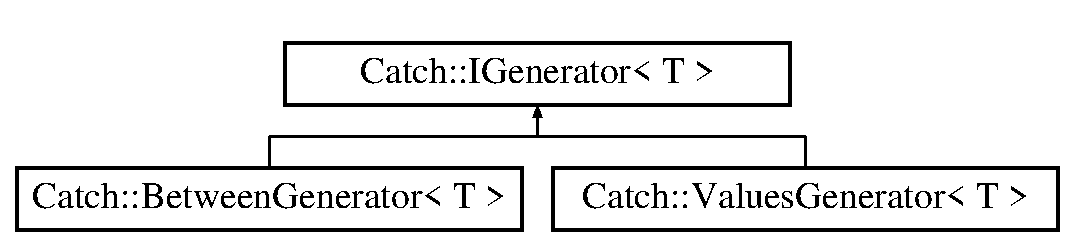
\includegraphics[height=2.000000cm]{structCatch_1_1IGenerator}
\end{center}
\end{figure}
\subsubsection*{Public Member Functions}
\begin{DoxyCompactItemize}
\item 
virtual \hyperlink{structCatch_1_1IGenerator_a0622037f4617e09aa8c584b0144d4a1a}{$\sim$\-I\-Generator} ()
\item 
virtual T \hyperlink{structCatch_1_1IGenerator_ad69e937cb66dba3ed9429c42abf4fce3}{get\-Value} (std\-::size\-\_\-t index) const =0
\item 
virtual std\-::size\-\_\-t \hyperlink{structCatch_1_1IGenerator_a2e317253b03e838b6065ce69719a198e}{size} () const =0
\end{DoxyCompactItemize}


\subsubsection{Constructor \& Destructor Documentation}
\hypertarget{structCatch_1_1IGenerator_a0622037f4617e09aa8c584b0144d4a1a}{\index{Catch\-::\-I\-Generator@{Catch\-::\-I\-Generator}!$\sim$\-I\-Generator@{$\sim$\-I\-Generator}}
\index{$\sim$\-I\-Generator@{$\sim$\-I\-Generator}!Catch::IGenerator@{Catch\-::\-I\-Generator}}
\paragraph[{$\sim$\-I\-Generator}]{\setlength{\rightskip}{0pt plus 5cm}template$<$typename T$>$ virtual {\bf Catch\-::\-I\-Generator}$<$ T $>$\-::$\sim${\bf I\-Generator} (
\begin{DoxyParamCaption}
{}
\end{DoxyParamCaption}
)\hspace{0.3cm}{\ttfamily [inline]}, {\ttfamily [virtual]}}}\label{structCatch_1_1IGenerator_a0622037f4617e09aa8c584b0144d4a1a}


\subsubsection{Member Function Documentation}
\hypertarget{structCatch_1_1IGenerator_ad69e937cb66dba3ed9429c42abf4fce3}{\index{Catch\-::\-I\-Generator@{Catch\-::\-I\-Generator}!get\-Value@{get\-Value}}
\index{get\-Value@{get\-Value}!Catch::IGenerator@{Catch\-::\-I\-Generator}}
\paragraph[{get\-Value}]{\setlength{\rightskip}{0pt plus 5cm}template$<$typename T$>$ virtual T {\bf Catch\-::\-I\-Generator}$<$ T $>$\-::get\-Value (
\begin{DoxyParamCaption}
\item[{std\-::size\-\_\-t}]{index}
\end{DoxyParamCaption}
) const\hspace{0.3cm}{\ttfamily [pure virtual]}}}\label{structCatch_1_1IGenerator_ad69e937cb66dba3ed9429c42abf4fce3}


Implemented in \hyperlink{classCatch_1_1ValuesGenerator_a60599dd67096ff108471f64ee42acd9d}{Catch\-::\-Values\-Generator$<$ T $>$}, and \hyperlink{classCatch_1_1BetweenGenerator_af83575d62cc727ca995446cff4d6c26c}{Catch\-::\-Between\-Generator$<$ T $>$}.

\hypertarget{structCatch_1_1IGenerator_a2e317253b03e838b6065ce69719a198e}{\index{Catch\-::\-I\-Generator@{Catch\-::\-I\-Generator}!size@{size}}
\index{size@{size}!Catch::IGenerator@{Catch\-::\-I\-Generator}}
\paragraph[{size}]{\setlength{\rightskip}{0pt plus 5cm}template$<$typename T$>$ virtual std\-::size\-\_\-t {\bf Catch\-::\-I\-Generator}$<$ T $>$\-::size (
\begin{DoxyParamCaption}
{}
\end{DoxyParamCaption}
) const\hspace{0.3cm}{\ttfamily [pure virtual]}}}\label{structCatch_1_1IGenerator_a2e317253b03e838b6065ce69719a198e}


Implemented in \hyperlink{classCatch_1_1ValuesGenerator_a98a80bb0dd682c44e82e4a75e98c4682}{Catch\-::\-Values\-Generator$<$ T $>$}, and \hyperlink{classCatch_1_1BetweenGenerator_aa53a04a259e796ba2b5adabed79474b5}{Catch\-::\-Between\-Generator$<$ T $>$}.



The documentation for this struct was generated from the following file\-:\begin{DoxyCompactItemize}
\item 
include/\hyperlink{catch_8hpp}{catch.\-hpp}\end{DoxyCompactItemize}

\hypertarget{structCatch_1_1IMutableContext}{\subsection{Catch\-:\-:I\-Mutable\-Context Struct Reference}
\label{structCatch_1_1IMutableContext}\index{Catch\-::\-I\-Mutable\-Context@{Catch\-::\-I\-Mutable\-Context}}
}


{\ttfamily \#include $<$catch.\-hpp$>$}

Inheritance diagram for Catch\-:\-:I\-Mutable\-Context\-:\begin{figure}[H]
\begin{center}
\leavevmode
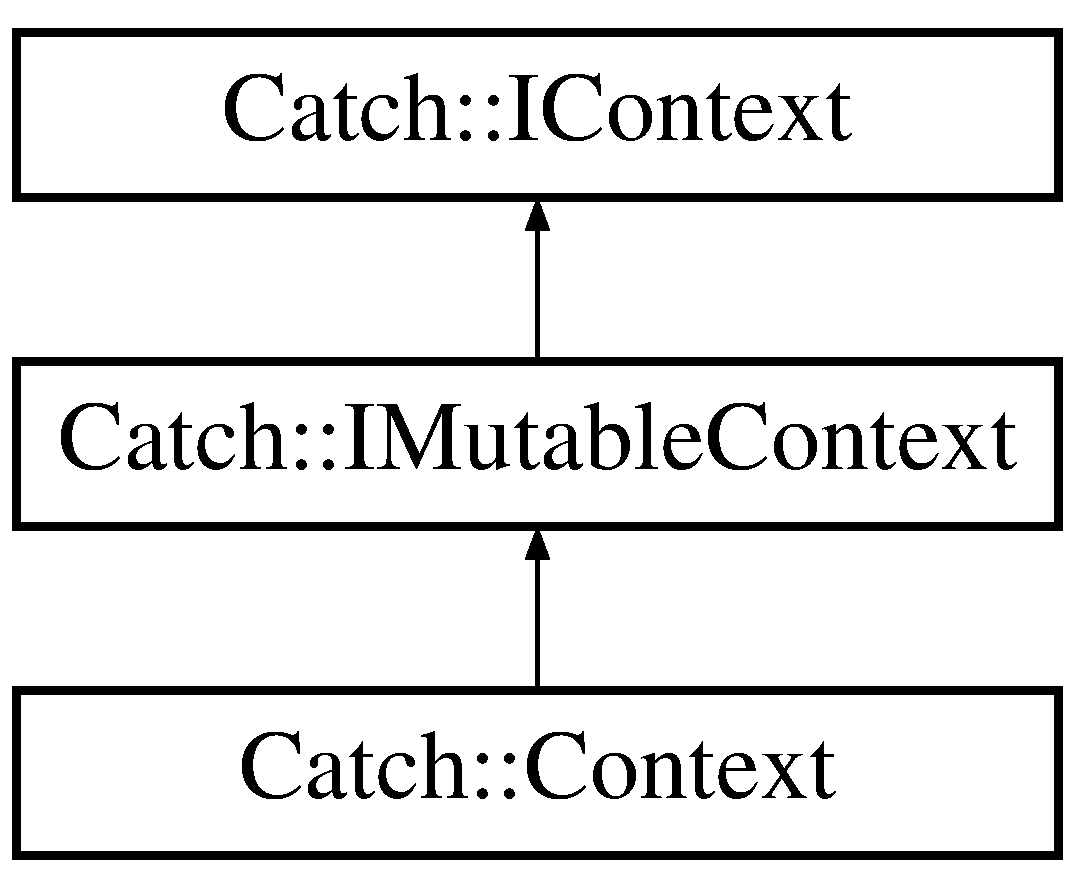
\includegraphics[height=3.000000cm]{structCatch_1_1IMutableContext}
\end{center}
\end{figure}
\subsubsection*{Public Member Functions}
\begin{DoxyCompactItemize}
\item 
virtual void \hyperlink{structCatch_1_1IMutableContext_a4a80afd0525b7def21bee8d9b48f2d39}{set\-Result\-Capture} (\hyperlink{structCatch_1_1IResultCapture}{I\-Result\-Capture} $\ast$result\-Capture)=0
\item 
virtual void \hyperlink{structCatch_1_1IMutableContext_af2e53b1dea4527a2587cff266a730f6e}{set\-Runner} (\hyperlink{structCatch_1_1IRunner}{I\-Runner} $\ast$runner)=0
\item 
virtual void \hyperlink{structCatch_1_1IMutableContext_a6b9bea96de1a6a5c8d0f5b048a356d4c}{set\-Config} (const \hyperlink{structCatch_1_1IConfig}{I\-Config} $\ast$config)=0
\end{DoxyCompactItemize}


\subsubsection{Member Function Documentation}
\hypertarget{structCatch_1_1IMutableContext_a6b9bea96de1a6a5c8d0f5b048a356d4c}{\index{Catch\-::\-I\-Mutable\-Context@{Catch\-::\-I\-Mutable\-Context}!set\-Config@{set\-Config}}
\index{set\-Config@{set\-Config}!Catch::IMutableContext@{Catch\-::\-I\-Mutable\-Context}}
\paragraph[{set\-Config}]{\setlength{\rightskip}{0pt plus 5cm}virtual void Catch\-::\-I\-Mutable\-Context\-::set\-Config (
\begin{DoxyParamCaption}
\item[{const {\bf I\-Config} $\ast$}]{config}
\end{DoxyParamCaption}
)\hspace{0.3cm}{\ttfamily [pure virtual]}}}\label{structCatch_1_1IMutableContext_a6b9bea96de1a6a5c8d0f5b048a356d4c}


Implemented in \hyperlink{classCatch_1_1Context_a95379b3aeaca34fb2c9a7a4424cab98c}{Catch\-::\-Context}.

\hypertarget{structCatch_1_1IMutableContext_a4a80afd0525b7def21bee8d9b48f2d39}{\index{Catch\-::\-I\-Mutable\-Context@{Catch\-::\-I\-Mutable\-Context}!set\-Result\-Capture@{set\-Result\-Capture}}
\index{set\-Result\-Capture@{set\-Result\-Capture}!Catch::IMutableContext@{Catch\-::\-I\-Mutable\-Context}}
\paragraph[{set\-Result\-Capture}]{\setlength{\rightskip}{0pt plus 5cm}virtual void Catch\-::\-I\-Mutable\-Context\-::set\-Result\-Capture (
\begin{DoxyParamCaption}
\item[{{\bf I\-Result\-Capture} $\ast$}]{result\-Capture}
\end{DoxyParamCaption}
)\hspace{0.3cm}{\ttfamily [pure virtual]}}}\label{structCatch_1_1IMutableContext_a4a80afd0525b7def21bee8d9b48f2d39}


Implemented in \hyperlink{classCatch_1_1Context_acd5a98f515e43085a2d32e6c48d582b0}{Catch\-::\-Context}.

\hypertarget{structCatch_1_1IMutableContext_af2e53b1dea4527a2587cff266a730f6e}{\index{Catch\-::\-I\-Mutable\-Context@{Catch\-::\-I\-Mutable\-Context}!set\-Runner@{set\-Runner}}
\index{set\-Runner@{set\-Runner}!Catch::IMutableContext@{Catch\-::\-I\-Mutable\-Context}}
\paragraph[{set\-Runner}]{\setlength{\rightskip}{0pt plus 5cm}virtual void Catch\-::\-I\-Mutable\-Context\-::set\-Runner (
\begin{DoxyParamCaption}
\item[{{\bf I\-Runner} $\ast$}]{runner}
\end{DoxyParamCaption}
)\hspace{0.3cm}{\ttfamily [pure virtual]}}}\label{structCatch_1_1IMutableContext_af2e53b1dea4527a2587cff266a730f6e}


Implemented in \hyperlink{classCatch_1_1Context_a9be76af925623d87d5692a08bf58abca}{Catch\-::\-Context}.



The documentation for this struct was generated from the following file\-:\begin{DoxyCompactItemize}
\item 
include/\hyperlink{catch_8hpp}{catch.\-hpp}\end{DoxyCompactItemize}

\hypertarget{classevents_1_1Interaction}{\subsection{events.\-Interaction Class Reference}
\label{classevents_1_1Interaction}\index{events.\-Interaction@{events.\-Interaction}}
}
Inheritance diagram for events.\-Interaction\-:\begin{figure}[H]
\begin{center}
\leavevmode
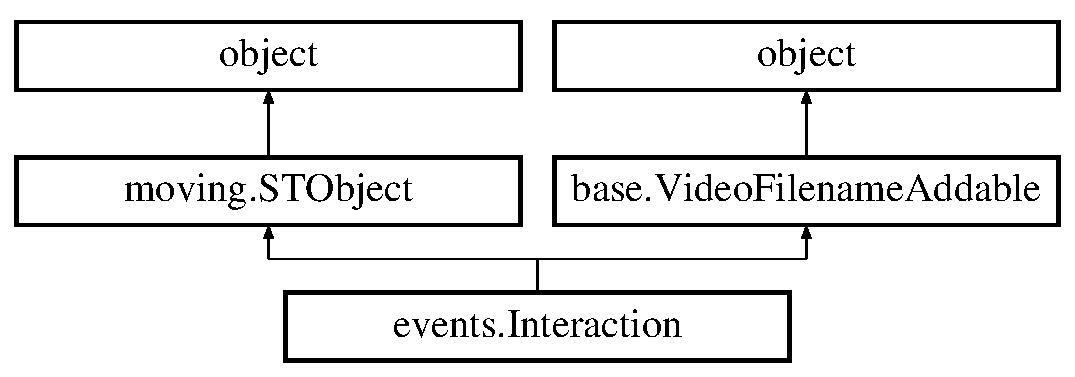
\includegraphics[height=3.000000cm]{classevents_1_1Interaction}
\end{center}
\end{figure}
\subsubsection*{Public Member Functions}
\begin{DoxyCompactItemize}
\item 
def \hyperlink{classevents_1_1Interaction_a37d41fbb1e5ce875dbc6c02f3a9d779c}{\-\_\-\-\_\-init\-\_\-\-\_\-}
\item 
def \hyperlink{classevents_1_1Interaction_a36254aa076f56784f9d48c08b6d48754}{get\-Road\-User\-Numbers}
\item 
def \hyperlink{classevents_1_1Interaction_a12448cfb45e896ab1c63aadbc61d2d9e}{set\-Road\-Users}
\item 
def \hyperlink{classevents_1_1Interaction_aa2e48b903c06f68adcde188f19155836}{get\-Indicator}
\item 
def \hyperlink{classevents_1_1Interaction_a3d1a455dc3f234458006f169ede1fafb}{add\-Indicator}
\item 
def \hyperlink{classevents_1_1Interaction_a3807a9d1f7a2bcc647855a2b8220c321}{get\-Indicator\-Value\-At\-Instant}
\item 
def \hyperlink{classevents_1_1Interaction_adb1c68b44b3ad0f002b4c4c4f2ac1411}{get\-Indicator\-Values\-At\-Instant}
\item 
def \hyperlink{classevents_1_1Interaction_a9639481ee2d4c7f9df61b24ca1402db8}{plot}
\item 
def \hyperlink{classevents_1_1Interaction_a6dfc8dd7cf05006aae65c13cd92c143e}{plot\-On\-World\-Image}
\item 
def \hyperlink{classevents_1_1Interaction_a49cbcbcec2428d0192974da932521821}{play}
\item 
def \hyperlink{classevents_1_1Interaction_a88bd165a8d768cbcf5aa599bd2595745}{compute\-Indicators}
\item 
def \hyperlink{classevents_1_1Interaction_a124a52882242e2fe699d9200e7fcd5c7}{compute\-Crossings\-Collisions}
\item 
def \hyperlink{classevents_1_1Interaction_a27e9ec43d8dc83490624669bea0db810}{compute\-P\-E\-T}
\item 
def \hyperlink{classevents_1_1Interaction_a4c4a705ecb073cf6d3e26fa433d0522b}{set\-Collision}
\item 
def \hyperlink{classevents_1_1Interaction_a5f8a88ad27c73937bcdc9935435c5e34}{is\-Collision}
\item 
def \hyperlink{classevents_1_1Interaction_a54d2c75ee1f805438ccf5427908c0e99}{get\-Collision\-Points}
\item 
def \hyperlink{classevents_1_1Interaction_a49ae1e32f056c6404678ca0ec5ee09b4}{get\-Crossing\-Zones}
\end{DoxyCompactItemize}
\subsubsection*{Public Attributes}
\begin{DoxyCompactItemize}
\item 
\hyperlink{classevents_1_1Interaction_acd9ac2aa2b8a71bb1718a3ee5899018b}{time\-Interval}
\item 
\hyperlink{classevents_1_1Interaction_a9a04846f8cf171f10f28d7eeb225d4be}{road\-User1}
\item 
\hyperlink{classevents_1_1Interaction_a65694843a89a3c452dd88e5a5f42a81e}{road\-User2}
\item 
\hyperlink{classevents_1_1Interaction_a9b1791b28fc1fce202bcd20ae43165cd}{road\-User\-Numbers}
\item 
\hyperlink{classevents_1_1Interaction_a151a6e0a5240a1f59d6210502c12d3cd}{category\-Num}
\item 
\hyperlink{classevents_1_1Interaction_a63550a0bfc7e2276b72ecaaf4958ab5e}{indicators}
\item 
\hyperlink{classevents_1_1Interaction_a25090186ae70b1e409228b7e4ed174b4}{interaction\-Interval}
\item 
\hyperlink{classevents_1_1Interaction_adcbf2b6e0bae45140323d94565c61354}{collision\-Points}
\item 
\hyperlink{classevents_1_1Interaction_aabeafe12aba2ff523496001e85042e51}{crossing\-Zones}
\item 
\hyperlink{classevents_1_1Interaction_a21c2eb7375a31ee4d6dd2ede7be622ae}{pet}
\item 
\hyperlink{classevents_1_1Interaction_a542128c09df1352263c53fd059a5b190}{collision}
\end{DoxyCompactItemize}
\subsubsection*{Static Public Attributes}
\begin{DoxyCompactItemize}
\item 
dictionary \hyperlink{classevents_1_1Interaction_af006771e67847af6c5ca1f8f7fa46a3d}{categories}
\item 
list \hyperlink{classevents_1_1Interaction_a573cc05c1d659e0d5912b3eb2361d43f}{indicator\-Names}
\item 
tuple \hyperlink{classevents_1_1Interaction_aed1115f38b9e2d6154ffa22d4c3c3455}{indicator\-Name\-To\-Indices} = \hyperlink{namespaceutils_ad6e2839437b1cc265f6c89f24780e3de}{utils.\-inverse\-Enumeration}(\hyperlink{classevents_1_1Interaction_a573cc05c1d659e0d5912b3eb2361d43f}{indicator\-Names})
\item 
list \hyperlink{classevents_1_1Interaction_a85329e433b60d0b41c12c51634ff95fa}{indicator\-Short\-Names}
\item 
list \hyperlink{classevents_1_1Interaction_aab56132b6523d94fd27317ebeb1e7fd2}{indicator\-Units}
\item 
list \hyperlink{classevents_1_1Interaction_a4925b91d8a26d5f6e6e7e488009ed5ad}{time\-Indicators} = \mbox{[}'Time to Collision', 'predicted Post Encroachment Time'\mbox{]}
\end{DoxyCompactItemize}


\subsubsection{Detailed Description}
\begin{DoxyVerb}Class for an interaction between two road users 
or a road user and an obstacle

link to the moving objects
contains the indicators in a dictionary with the names as keys
\end{DoxyVerb}
 

\subsubsection{Constructor \& Destructor Documentation}
\hypertarget{classevents_1_1Interaction_a37d41fbb1e5ce875dbc6c02f3a9d779c}{\index{events\-::\-Interaction@{events\-::\-Interaction}!\-\_\-\-\_\-init\-\_\-\-\_\-@{\-\_\-\-\_\-init\-\_\-\-\_\-}}
\index{\-\_\-\-\_\-init\-\_\-\-\_\-@{\-\_\-\-\_\-init\-\_\-\-\_\-}!events::Interaction@{events\-::\-Interaction}}
\paragraph[{\-\_\-\-\_\-init\-\_\-\-\_\-}]{\setlength{\rightskip}{0pt plus 5cm}def events.\-Interaction.\-\_\-\-\_\-init\-\_\-\-\_\- (
\begin{DoxyParamCaption}
\item[{}]{self, }
\item[{}]{num = {\ttfamily None}, }
\item[{}]{time\-Interval = {\ttfamily None}, }
\item[{}]{roaduser\-Num1 = {\ttfamily None}, }
\item[{}]{roaduser\-Num2 = {\ttfamily None}, }
\item[{}]{road\-User1 = {\ttfamily None}, }
\item[{}]{road\-User2 = {\ttfamily None}, }
\item[{}]{category\-Num = {\ttfamily None}}
\end{DoxyParamCaption}
)}}\label{classevents_1_1Interaction_a37d41fbb1e5ce875dbc6c02f3a9d779c}


References moving.\-S\-T\-Object.\-\_\-\-\_\-init\-\_\-\-\_\-().



\subsubsection{Member Function Documentation}
\hypertarget{classevents_1_1Interaction_a3d1a455dc3f234458006f169ede1fafb}{\index{events\-::\-Interaction@{events\-::\-Interaction}!add\-Indicator@{add\-Indicator}}
\index{add\-Indicator@{add\-Indicator}!events::Interaction@{events\-::\-Interaction}}
\paragraph[{add\-Indicator}]{\setlength{\rightskip}{0pt plus 5cm}def events.\-Interaction.\-add\-Indicator (
\begin{DoxyParamCaption}
\item[{}]{self, }
\item[{}]{indicator}
\end{DoxyParamCaption}
)}}\label{classevents_1_1Interaction_a3d1a455dc3f234458006f169ede1fafb}


References events.\-Interaction.\-indicators.

\hypertarget{classevents_1_1Interaction_a124a52882242e2fe699d9200e7fcd5c7}{\index{events\-::\-Interaction@{events\-::\-Interaction}!compute\-Crossings\-Collisions@{compute\-Crossings\-Collisions}}
\index{compute\-Crossings\-Collisions@{compute\-Crossings\-Collisions}!events::Interaction@{events\-::\-Interaction}}
\paragraph[{compute\-Crossings\-Collisions}]{\setlength{\rightskip}{0pt plus 5cm}def events.\-Interaction.\-compute\-Crossings\-Collisions (
\begin{DoxyParamCaption}
\item[{}]{self, }
\item[{}]{prediction\-Parameters, }
\item[{}]{collision\-Distance\-Threshold, }
\item[{}]{time\-Horizon, }
\item[{}]{compute\-C\-Z = {\ttfamily False}, }
\item[{}]{debug = {\ttfamily False}, }
\item[{}]{time\-Interval = {\ttfamily None}, }
\item[{}]{n\-Processes = {\ttfamily 1}, }
\item[{}]{use\-Prototypes = {\ttfamily False}, }
\item[{}]{route1 = {\ttfamily (-\/1,-\/1}, }
\item[{}]{route2 = {\ttfamily (-\/1,-\/1}, }
\item[{}]{prototypes = {\ttfamily \{\}}, }
\item[{}]{second\-Step\-Prototypes = {\ttfamily \{\}}, }
\item[{}]{n\-Matching = {\ttfamily \{\}}, }
\item[{}]{objects = {\ttfamily \mbox{[}\mbox{]}}, }
\item[{}]{noise\-Entry\-Nums = {\ttfamily \mbox{[}\mbox{]}}, }
\item[{}]{noise\-Exit\-Nums = {\ttfamily \mbox{[}\mbox{]}}, }
\item[{}]{min\-Similarity = {\ttfamily 0.1}, }
\item[{}]{most\-Matched = {\ttfamily None}, }
\item[{}]{use\-Destination = {\ttfamily True}, }
\item[{}]{use\-Speed\-Prototype = {\ttfamily True}, }
\item[{}]{accept\-Partial\-Length = {\ttfamily 30}, }
\item[{}]{step = {\ttfamily 1}}
\end{DoxyParamCaption}
)}}\label{classevents_1_1Interaction_a124a52882242e2fe699d9200e7fcd5c7}
\begin{DoxyVerb}Computes all crossing and collision points at each common instant for two road users. \end{DoxyVerb}
 

References events.\-Interaction.\-add\-Indicator(), events.\-Interaction.\-collision\-Points, prediction.\-Safety\-Point.\-compute\-Expected\-Indicator(), K\-L\-T\-Feature\-Tracking\-Parameters.\-crossing\-Zones, events.\-Interaction.\-crossing\-Zones, events.\-get\-Route(), events.\-Interaction.\-road\-User1, events.\-Interaction.\-road\-User2, and events.\-Interaction.\-time\-Interval.

\hypertarget{classevents_1_1Interaction_a88bd165a8d768cbcf5aa599bd2595745}{\index{events\-::\-Interaction@{events\-::\-Interaction}!compute\-Indicators@{compute\-Indicators}}
\index{compute\-Indicators@{compute\-Indicators}!events::Interaction@{events\-::\-Interaction}}
\paragraph[{compute\-Indicators}]{\setlength{\rightskip}{0pt plus 5cm}def events.\-Interaction.\-compute\-Indicators (
\begin{DoxyParamCaption}
\item[{}]{self}
\end{DoxyParamCaption}
)}}\label{classevents_1_1Interaction_a88bd165a8d768cbcf5aa599bd2595745}
\begin{DoxyVerb}Computes the collision course cosine only if the cosine is positive\end{DoxyVerb}
 

References events.\-Interaction.\-add\-Indicator(), moving.\-Point.\-dot(), events.\-Interaction.\-interaction\-Interval, moving.\-Moving\-Object.\-min\-Distance(), events.\-Interaction.\-road\-User1, events.\-Interaction.\-road\-User2, and events.\-Interaction.\-time\-Interval.

\hypertarget{classevents_1_1Interaction_a27e9ec43d8dc83490624669bea0db810}{\index{events\-::\-Interaction@{events\-::\-Interaction}!compute\-P\-E\-T@{compute\-P\-E\-T}}
\index{compute\-P\-E\-T@{compute\-P\-E\-T}!events::Interaction@{events\-::\-Interaction}}
\paragraph[{compute\-P\-E\-T}]{\setlength{\rightskip}{0pt plus 5cm}def events.\-Interaction.\-compute\-P\-E\-T (
\begin{DoxyParamCaption}
\item[{}]{self, }
\item[{}]{collision\-Distance\-Threshold}
\end{DoxyParamCaption}
)}}\label{classevents_1_1Interaction_a27e9ec43d8dc83490624669bea0db810}
\hypertarget{classevents_1_1Interaction_a54d2c75ee1f805438ccf5427908c0e99}{\index{events\-::\-Interaction@{events\-::\-Interaction}!get\-Collision\-Points@{get\-Collision\-Points}}
\index{get\-Collision\-Points@{get\-Collision\-Points}!events::Interaction@{events\-::\-Interaction}}
\paragraph[{get\-Collision\-Points}]{\setlength{\rightskip}{0pt plus 5cm}def events.\-Interaction.\-get\-Collision\-Points (
\begin{DoxyParamCaption}
\item[{}]{self}
\end{DoxyParamCaption}
)}}\label{classevents_1_1Interaction_a54d2c75ee1f805438ccf5427908c0e99}


References events.\-Interaction.\-collision\-Points.

\hypertarget{classevents_1_1Interaction_a49ae1e32f056c6404678ca0ec5ee09b4}{\index{events\-::\-Interaction@{events\-::\-Interaction}!get\-Crossing\-Zones@{get\-Crossing\-Zones}}
\index{get\-Crossing\-Zones@{get\-Crossing\-Zones}!events::Interaction@{events\-::\-Interaction}}
\paragraph[{get\-Crossing\-Zones}]{\setlength{\rightskip}{0pt plus 5cm}def events.\-Interaction.\-get\-Crossing\-Zones (
\begin{DoxyParamCaption}
\item[{}]{self}
\end{DoxyParamCaption}
)}}\label{classevents_1_1Interaction_a49ae1e32f056c6404678ca0ec5ee09b4}


References K\-L\-T\-Feature\-Tracking\-Parameters.\-crossing\-Zones, and events.\-Interaction.\-crossing\-Zones.

\hypertarget{classevents_1_1Interaction_aa2e48b903c06f68adcde188f19155836}{\index{events\-::\-Interaction@{events\-::\-Interaction}!get\-Indicator@{get\-Indicator}}
\index{get\-Indicator@{get\-Indicator}!events::Interaction@{events\-::\-Interaction}}
\paragraph[{get\-Indicator}]{\setlength{\rightskip}{0pt plus 5cm}def events.\-Interaction.\-get\-Indicator (
\begin{DoxyParamCaption}
\item[{}]{self, }
\item[{}]{indicator\-Name}
\end{DoxyParamCaption}
)}}\label{classevents_1_1Interaction_aa2e48b903c06f68adcde188f19155836}
\hypertarget{classevents_1_1Interaction_a3807a9d1f7a2bcc647855a2b8220c321}{\index{events\-::\-Interaction@{events\-::\-Interaction}!get\-Indicator\-Value\-At\-Instant@{get\-Indicator\-Value\-At\-Instant}}
\index{get\-Indicator\-Value\-At\-Instant@{get\-Indicator\-Value\-At\-Instant}!events::Interaction@{events\-::\-Interaction}}
\paragraph[{get\-Indicator\-Value\-At\-Instant}]{\setlength{\rightskip}{0pt plus 5cm}def events.\-Interaction.\-get\-Indicator\-Value\-At\-Instant (
\begin{DoxyParamCaption}
\item[{}]{self, }
\item[{}]{indicator\-Name, }
\item[{}]{instant}
\end{DoxyParamCaption}
)}}\label{classevents_1_1Interaction_a3807a9d1f7a2bcc647855a2b8220c321}


References events.\-Interaction.\-get\-Indicator().

\hypertarget{classevents_1_1Interaction_adb1c68b44b3ad0f002b4c4c4f2ac1411}{\index{events\-::\-Interaction@{events\-::\-Interaction}!get\-Indicator\-Values\-At\-Instant@{get\-Indicator\-Values\-At\-Instant}}
\index{get\-Indicator\-Values\-At\-Instant@{get\-Indicator\-Values\-At\-Instant}!events::Interaction@{events\-::\-Interaction}}
\paragraph[{get\-Indicator\-Values\-At\-Instant}]{\setlength{\rightskip}{0pt plus 5cm}def events.\-Interaction.\-get\-Indicator\-Values\-At\-Instant (
\begin{DoxyParamCaption}
\item[{}]{self, }
\item[{}]{instant}
\end{DoxyParamCaption}
)}}\label{classevents_1_1Interaction_adb1c68b44b3ad0f002b4c4c4f2ac1411}
\begin{DoxyVerb}Returns list of indicator values at instant
as dict (with keys from indicators dict)\end{DoxyVerb}
 \hypertarget{classevents_1_1Interaction_a36254aa076f56784f9d48c08b6d48754}{\index{events\-::\-Interaction@{events\-::\-Interaction}!get\-Road\-User\-Numbers@{get\-Road\-User\-Numbers}}
\index{get\-Road\-User\-Numbers@{get\-Road\-User\-Numbers}!events::Interaction@{events\-::\-Interaction}}
\paragraph[{get\-Road\-User\-Numbers}]{\setlength{\rightskip}{0pt plus 5cm}def events.\-Interaction.\-get\-Road\-User\-Numbers (
\begin{DoxyParamCaption}
\item[{}]{self}
\end{DoxyParamCaption}
)}}\label{classevents_1_1Interaction_a36254aa076f56784f9d48c08b6d48754}


References events.\-Interaction.\-road\-User\-Numbers.

\hypertarget{classevents_1_1Interaction_a5f8a88ad27c73937bcdc9935435c5e34}{\index{events\-::\-Interaction@{events\-::\-Interaction}!is\-Collision@{is\-Collision}}
\index{is\-Collision@{is\-Collision}!events::Interaction@{events\-::\-Interaction}}
\paragraph[{is\-Collision}]{\setlength{\rightskip}{0pt plus 5cm}def events.\-Interaction.\-is\-Collision (
\begin{DoxyParamCaption}
\item[{}]{self}
\end{DoxyParamCaption}
)}}\label{classevents_1_1Interaction_a5f8a88ad27c73937bcdc9935435c5e34}


References events.\-Interaction.\-collision.

\hypertarget{classevents_1_1Interaction_a49cbcbcec2428d0192974da932521821}{\index{events\-::\-Interaction@{events\-::\-Interaction}!play@{play}}
\index{play@{play}!events::Interaction@{events\-::\-Interaction}}
\paragraph[{play}]{\setlength{\rightskip}{0pt plus 5cm}def events.\-Interaction.\-play (
\begin{DoxyParamCaption}
\item[{}]{self, }
\item[{}]{video\-Filename, }
\item[{}]{homography = {\ttfamily None}, }
\item[{}]{undistort = {\ttfamily False}, }
\item[{}]{intrinsic\-Camera\-Matrix = {\ttfamily None}, }
\item[{}]{distortion\-Coefficients = {\ttfamily None}, }
\item[{}]{undistorted\-Image\-Multiplication = {\ttfamily 1.}}
\end{DoxyParamCaption}
)}}\label{classevents_1_1Interaction_a49cbcbcec2428d0192974da932521821}


References cvutils.\-display\-Trajectories(), Feature\-Trajectory.\-get\-First\-Instant(), moving.\-S\-T\-Object.\-get\-First\-Instant(), Feature\-Trajectory.\-get\-Last\-Instant(), moving.\-S\-T\-Object.\-get\-Last\-Instant(), events.\-Interaction.\-road\-User1, and events.\-Interaction.\-road\-User2.

\hypertarget{classevents_1_1Interaction_a9639481ee2d4c7f9df61b24ca1402db8}{\index{events\-::\-Interaction@{events\-::\-Interaction}!plot@{plot}}
\index{plot@{plot}!events::Interaction@{events\-::\-Interaction}}
\paragraph[{plot}]{\setlength{\rightskip}{0pt plus 5cm}def events.\-Interaction.\-plot (
\begin{DoxyParamCaption}
\item[{}]{self, }
\item[{}]{options = {\ttfamily ''}, }
\item[{}]{with\-Origin = {\ttfamily False}, }
\item[{}]{time\-Step = {\ttfamily 1}, }
\item[{}]{with\-Features = {\ttfamily False}, }
\item[{}]{kwargs}
\end{DoxyParamCaption}
)}}\label{classevents_1_1Interaction_a9639481ee2d4c7f9df61b24ca1402db8}
\hypertarget{classevents_1_1Interaction_a6dfc8dd7cf05006aae65c13cd92c143e}{\index{events\-::\-Interaction@{events\-::\-Interaction}!plot\-On\-World\-Image@{plot\-On\-World\-Image}}
\index{plot\-On\-World\-Image@{plot\-On\-World\-Image}!events::Interaction@{events\-::\-Interaction}}
\paragraph[{plot\-On\-World\-Image}]{\setlength{\rightskip}{0pt plus 5cm}def events.\-Interaction.\-plot\-On\-World\-Image (
\begin{DoxyParamCaption}
\item[{}]{self, }
\item[{}]{n\-Pixels\-Per\-Unit\-Distance, }
\item[{}]{options = {\ttfamily ''}, }
\item[{}]{with\-Origin = {\ttfamily False}, }
\item[{}]{time\-Step = {\ttfamily 1}, }
\item[{}]{kwargs}
\end{DoxyParamCaption}
)}}\label{classevents_1_1Interaction_a6dfc8dd7cf05006aae65c13cd92c143e}
\hypertarget{classevents_1_1Interaction_a4c4a705ecb073cf6d3e26fa433d0522b}{\index{events\-::\-Interaction@{events\-::\-Interaction}!set\-Collision@{set\-Collision}}
\index{set\-Collision@{set\-Collision}!events::Interaction@{events\-::\-Interaction}}
\paragraph[{set\-Collision}]{\setlength{\rightskip}{0pt plus 5cm}def events.\-Interaction.\-set\-Collision (
\begin{DoxyParamCaption}
\item[{}]{self, }
\item[{}]{collision}
\end{DoxyParamCaption}
)}}\label{classevents_1_1Interaction_a4c4a705ecb073cf6d3e26fa433d0522b}
\begin{DoxyVerb}indicates if it is a collision: argument should be boolean\end{DoxyVerb}
 \hypertarget{classevents_1_1Interaction_a12448cfb45e896ab1c63aadbc61d2d9e}{\index{events\-::\-Interaction@{events\-::\-Interaction}!set\-Road\-Users@{set\-Road\-Users}}
\index{set\-Road\-Users@{set\-Road\-Users}!events::Interaction@{events\-::\-Interaction}}
\paragraph[{set\-Road\-Users}]{\setlength{\rightskip}{0pt plus 5cm}def events.\-Interaction.\-set\-Road\-Users (
\begin{DoxyParamCaption}
\item[{}]{self, }
\item[{}]{objects}
\end{DoxyParamCaption}
)}}\label{classevents_1_1Interaction_a12448cfb45e896ab1c63aadbc61d2d9e}


References moving.\-S\-T\-Object.\-get\-Num(), events.\-Interaction.\-get\-Road\-User\-Numbers(), events.\-Interaction.\-road\-User1, and events.\-Interaction.\-road\-User2.



\subsubsection{Member Data Documentation}
\hypertarget{classevents_1_1Interaction_af006771e67847af6c5ca1f8f7fa46a3d}{\index{events\-::\-Interaction@{events\-::\-Interaction}!categories@{categories}}
\index{categories@{categories}!events::Interaction@{events\-::\-Interaction}}
\paragraph[{categories}]{\setlength{\rightskip}{0pt plus 5cm}dictionary events.\-Interaction.\-categories\hspace{0.3cm}{\ttfamily [static]}}}\label{classevents_1_1Interaction_af006771e67847af6c5ca1f8f7fa46a3d}
{\bfseries Initial value\-:}
\begin{DoxyCode}
1 = \{\textcolor{stringliteral}{'Head On'}: 0,
2                   \textcolor{stringliteral}{'rearend'}: 1,
3                   \textcolor{stringliteral}{'side'}: 2,
4                   \textcolor{stringliteral}{'parallel'}: 3\}
\end{DoxyCode}
\hypertarget{classevents_1_1Interaction_a151a6e0a5240a1f59d6210502c12d3cd}{\index{events\-::\-Interaction@{events\-::\-Interaction}!category\-Num@{category\-Num}}
\index{category\-Num@{category\-Num}!events::Interaction@{events\-::\-Interaction}}
\paragraph[{category\-Num}]{\setlength{\rightskip}{0pt plus 5cm}events.\-Interaction.\-category\-Num}}\label{classevents_1_1Interaction_a151a6e0a5240a1f59d6210502c12d3cd}
\hypertarget{classevents_1_1Interaction_a542128c09df1352263c53fd059a5b190}{\index{events\-::\-Interaction@{events\-::\-Interaction}!collision@{collision}}
\index{collision@{collision}!events::Interaction@{events\-::\-Interaction}}
\paragraph[{collision}]{\setlength{\rightskip}{0pt plus 5cm}events.\-Interaction.\-collision}}\label{classevents_1_1Interaction_a542128c09df1352263c53fd059a5b190}
\hypertarget{classevents_1_1Interaction_adcbf2b6e0bae45140323d94565c61354}{\index{events\-::\-Interaction@{events\-::\-Interaction}!collision\-Points@{collision\-Points}}
\index{collision\-Points@{collision\-Points}!events::Interaction@{events\-::\-Interaction}}
\paragraph[{collision\-Points}]{\setlength{\rightskip}{0pt plus 5cm}events.\-Interaction.\-collision\-Points}}\label{classevents_1_1Interaction_adcbf2b6e0bae45140323d94565c61354}
\hypertarget{classevents_1_1Interaction_aabeafe12aba2ff523496001e85042e51}{\index{events\-::\-Interaction@{events\-::\-Interaction}!crossing\-Zones@{crossing\-Zones}}
\index{crossing\-Zones@{crossing\-Zones}!events::Interaction@{events\-::\-Interaction}}
\paragraph[{crossing\-Zones}]{\setlength{\rightskip}{0pt plus 5cm}events.\-Interaction.\-crossing\-Zones}}\label{classevents_1_1Interaction_aabeafe12aba2ff523496001e85042e51}
\hypertarget{classevents_1_1Interaction_a573cc05c1d659e0d5912b3eb2361d43f}{\index{events\-::\-Interaction@{events\-::\-Interaction}!indicator\-Names@{indicator\-Names}}
\index{indicator\-Names@{indicator\-Names}!events::Interaction@{events\-::\-Interaction}}
\paragraph[{indicator\-Names}]{\setlength{\rightskip}{0pt plus 5cm}list events.\-Interaction.\-indicator\-Names\hspace{0.3cm}{\ttfamily [static]}}}\label{classevents_1_1Interaction_a573cc05c1d659e0d5912b3eb2361d43f}
{\bfseries Initial value\-:}
\begin{DoxyCode}
1 = [\textcolor{stringliteral}{'Collision Course Dot Product'},
2                       \textcolor{stringliteral}{'Collision Course Angle'},
3                       \textcolor{stringliteral}{'Distance'},
4                       \textcolor{stringliteral}{'Minimum Distance'},
5                       \textcolor{stringliteral}{'Velocity Angle'},
6                       \textcolor{stringliteral}{'Speed Differential'},
7                       \textcolor{stringliteral}{'Collision Probability'},
8                       \textcolor{stringliteral}{'Time to Collision'}, \textcolor{comment}{# 7}
9                       \textcolor{stringliteral}{'Probability of Successful Evasive Action'},
10                       \textcolor{stringliteral}{'predicted Post Encroachment Time'}]
\end{DoxyCode}
\hypertarget{classevents_1_1Interaction_aed1115f38b9e2d6154ffa22d4c3c3455}{\index{events\-::\-Interaction@{events\-::\-Interaction}!indicator\-Name\-To\-Indices@{indicator\-Name\-To\-Indices}}
\index{indicator\-Name\-To\-Indices@{indicator\-Name\-To\-Indices}!events::Interaction@{events\-::\-Interaction}}
\paragraph[{indicator\-Name\-To\-Indices}]{\setlength{\rightskip}{0pt plus 5cm}tuple events.\-Interaction.\-indicator\-Name\-To\-Indices = {\bf utils.\-inverse\-Enumeration}({\bf indicator\-Names})\hspace{0.3cm}{\ttfamily [static]}}}\label{classevents_1_1Interaction_aed1115f38b9e2d6154ffa22d4c3c3455}
\hypertarget{classevents_1_1Interaction_a63550a0bfc7e2276b72ecaaf4958ab5e}{\index{events\-::\-Interaction@{events\-::\-Interaction}!indicators@{indicators}}
\index{indicators@{indicators}!events::Interaction@{events\-::\-Interaction}}
\paragraph[{indicators}]{\setlength{\rightskip}{0pt plus 5cm}events.\-Interaction.\-indicators}}\label{classevents_1_1Interaction_a63550a0bfc7e2276b72ecaaf4958ab5e}
\hypertarget{classevents_1_1Interaction_a85329e433b60d0b41c12c51634ff95fa}{\index{events\-::\-Interaction@{events\-::\-Interaction}!indicator\-Short\-Names@{indicator\-Short\-Names}}
\index{indicator\-Short\-Names@{indicator\-Short\-Names}!events::Interaction@{events\-::\-Interaction}}
\paragraph[{indicator\-Short\-Names}]{\setlength{\rightskip}{0pt plus 5cm}list events.\-Interaction.\-indicator\-Short\-Names\hspace{0.3cm}{\ttfamily [static]}}}\label{classevents_1_1Interaction_a85329e433b60d0b41c12c51634ff95fa}
{\bfseries Initial value\-:}
\begin{DoxyCode}
1 = [\textcolor{stringliteral}{'CCDP'},
2                            \textcolor{stringliteral}{'CCA'},
3                            \textcolor{stringliteral}{'Dist'},
4                            \textcolor{stringliteral}{'MinDist'},
5                            \textcolor{stringliteral}{'VA'},
6                            \textcolor{stringliteral}{'SD'},
7                            \textcolor{stringliteral}{'PoC'},
8                            \textcolor{stringliteral}{'TTC'},
9                            \textcolor{stringliteral}{'P(SEA)'},
10                            \textcolor{stringliteral}{'pPET'}]
\end{DoxyCode}
\hypertarget{classevents_1_1Interaction_aab56132b6523d94fd27317ebeb1e7fd2}{\index{events\-::\-Interaction@{events\-::\-Interaction}!indicator\-Units@{indicator\-Units}}
\index{indicator\-Units@{indicator\-Units}!events::Interaction@{events\-::\-Interaction}}
\paragraph[{indicator\-Units}]{\setlength{\rightskip}{0pt plus 5cm}list events.\-Interaction.\-indicator\-Units\hspace{0.3cm}{\ttfamily [static]}}}\label{classevents_1_1Interaction_aab56132b6523d94fd27317ebeb1e7fd2}
{\bfseries Initial value\-:}
\begin{DoxyCode}
1 = [\textcolor{stringliteral}{''},
2                       \textcolor{stringliteral}{'rad'},
3                       \textcolor{stringliteral}{'m'},
4                       \textcolor{stringliteral}{'m'},
5                       \textcolor{stringliteral}{'rad'},
6                       \textcolor{stringliteral}{'m/s'},
7                       \textcolor{stringliteral}{''},
8                       \textcolor{stringliteral}{'s'},
9                       \textcolor{stringliteral}{''},
10                       \textcolor{stringliteral}{''}]
\end{DoxyCode}
\hypertarget{classevents_1_1Interaction_a25090186ae70b1e409228b7e4ed174b4}{\index{events\-::\-Interaction@{events\-::\-Interaction}!interaction\-Interval@{interaction\-Interval}}
\index{interaction\-Interval@{interaction\-Interval}!events::Interaction@{events\-::\-Interaction}}
\paragraph[{interaction\-Interval}]{\setlength{\rightskip}{0pt plus 5cm}events.\-Interaction.\-interaction\-Interval}}\label{classevents_1_1Interaction_a25090186ae70b1e409228b7e4ed174b4}
\hypertarget{classevents_1_1Interaction_a21c2eb7375a31ee4d6dd2ede7be622ae}{\index{events\-::\-Interaction@{events\-::\-Interaction}!pet@{pet}}
\index{pet@{pet}!events::Interaction@{events\-::\-Interaction}}
\paragraph[{pet}]{\setlength{\rightskip}{0pt plus 5cm}events.\-Interaction.\-pet}}\label{classevents_1_1Interaction_a21c2eb7375a31ee4d6dd2ede7be622ae}
\hypertarget{classevents_1_1Interaction_a9a04846f8cf171f10f28d7eeb225d4be}{\index{events\-::\-Interaction@{events\-::\-Interaction}!road\-User1@{road\-User1}}
\index{road\-User1@{road\-User1}!events::Interaction@{events\-::\-Interaction}}
\paragraph[{road\-User1}]{\setlength{\rightskip}{0pt plus 5cm}events.\-Interaction.\-road\-User1}}\label{classevents_1_1Interaction_a9a04846f8cf171f10f28d7eeb225d4be}
\hypertarget{classevents_1_1Interaction_a65694843a89a3c452dd88e5a5f42a81e}{\index{events\-::\-Interaction@{events\-::\-Interaction}!road\-User2@{road\-User2}}
\index{road\-User2@{road\-User2}!events::Interaction@{events\-::\-Interaction}}
\paragraph[{road\-User2}]{\setlength{\rightskip}{0pt plus 5cm}events.\-Interaction.\-road\-User2}}\label{classevents_1_1Interaction_a65694843a89a3c452dd88e5a5f42a81e}
\hypertarget{classevents_1_1Interaction_a9b1791b28fc1fce202bcd20ae43165cd}{\index{events\-::\-Interaction@{events\-::\-Interaction}!road\-User\-Numbers@{road\-User\-Numbers}}
\index{road\-User\-Numbers@{road\-User\-Numbers}!events::Interaction@{events\-::\-Interaction}}
\paragraph[{road\-User\-Numbers}]{\setlength{\rightskip}{0pt plus 5cm}events.\-Interaction.\-road\-User\-Numbers}}\label{classevents_1_1Interaction_a9b1791b28fc1fce202bcd20ae43165cd}
\hypertarget{classevents_1_1Interaction_a4925b91d8a26d5f6e6e7e488009ed5ad}{\index{events\-::\-Interaction@{events\-::\-Interaction}!time\-Indicators@{time\-Indicators}}
\index{time\-Indicators@{time\-Indicators}!events::Interaction@{events\-::\-Interaction}}
\paragraph[{time\-Indicators}]{\setlength{\rightskip}{0pt plus 5cm}list events.\-Interaction.\-time\-Indicators = \mbox{[}'Time to Collision', 'predicted Post Encroachment Time'\mbox{]}\hspace{0.3cm}{\ttfamily [static]}}}\label{classevents_1_1Interaction_a4925b91d8a26d5f6e6e7e488009ed5ad}
\hypertarget{classevents_1_1Interaction_acd9ac2aa2b8a71bb1718a3ee5899018b}{\index{events\-::\-Interaction@{events\-::\-Interaction}!time\-Interval@{time\-Interval}}
\index{time\-Interval@{time\-Interval}!events::Interaction@{events\-::\-Interaction}}
\paragraph[{time\-Interval}]{\setlength{\rightskip}{0pt plus 5cm}events.\-Interaction.\-time\-Interval}}\label{classevents_1_1Interaction_acd9ac2aa2b8a71bb1718a3ee5899018b}


The documentation for this class was generated from the following file\-:\begin{DoxyCompactItemize}
\item 
python/\hyperlink{events_8py}{events.\-py}\end{DoxyCompactItemize}

\hypertarget{classtraffic__engineering_1_1IntersectionMovement}{\subsection{traffic\-\_\-engineering.\-Intersection\-Movement Class Reference}
\label{classtraffic__engineering_1_1IntersectionMovement}\index{traffic\-\_\-engineering.\-Intersection\-Movement@{traffic\-\_\-engineering.\-Intersection\-Movement}}
}
Inheritance diagram for traffic\-\_\-engineering.\-Intersection\-Movement\-:\begin{figure}[H]
\begin{center}
\leavevmode
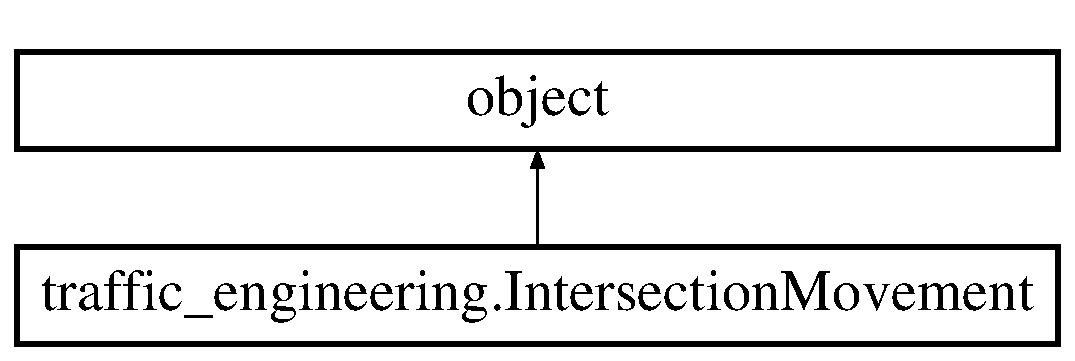
\includegraphics[height=2.000000cm]{classtraffic__engineering_1_1IntersectionMovement}
\end{center}
\end{figure}
\subsubsection*{Public Member Functions}
\begin{DoxyCompactItemize}
\item 
def \hyperlink{classtraffic__engineering_1_1IntersectionMovement_ae0d301b7637ad25e77683b637502d08a}{\-\_\-\-\_\-init\-\_\-\-\_\-}
\item 
def \hyperlink{classtraffic__engineering_1_1IntersectionMovement_afa688045995b9833ec1b7c5dbbc09de3}{get\-T\-V\-U\-Volume}
\end{DoxyCompactItemize}
\subsubsection*{Public Attributes}
\begin{DoxyCompactItemize}
\item 
\hyperlink{classtraffic__engineering_1_1IntersectionMovement_a57c9f52a7252a30f9e7859e8bcb8006c}{volume}
\item 
\hyperlink{classtraffic__engineering_1_1IntersectionMovement_acddb31d7563b35067734ae07faa10de0}{mvt\-Equivalent}
\end{DoxyCompactItemize}


\subsubsection{Detailed Description}
\begin{DoxyVerb}Represents an intersection movement
with a volume, a type (through, left or right)
and an equivalent for movement type\end{DoxyVerb}
 

\subsubsection{Constructor \& Destructor Documentation}
\hypertarget{classtraffic__engineering_1_1IntersectionMovement_ae0d301b7637ad25e77683b637502d08a}{\index{traffic\-\_\-engineering\-::\-Intersection\-Movement@{traffic\-\_\-engineering\-::\-Intersection\-Movement}!\-\_\-\-\_\-init\-\_\-\-\_\-@{\-\_\-\-\_\-init\-\_\-\-\_\-}}
\index{\-\_\-\-\_\-init\-\_\-\-\_\-@{\-\_\-\-\_\-init\-\_\-\-\_\-}!traffic_engineering::IntersectionMovement@{traffic\-\_\-engineering\-::\-Intersection\-Movement}}
\paragraph[{\-\_\-\-\_\-init\-\_\-\-\_\-}]{\setlength{\rightskip}{0pt plus 5cm}def traffic\-\_\-engineering.\-Intersection\-Movement.\-\_\-\-\_\-init\-\_\-\-\_\- (
\begin{DoxyParamCaption}
\item[{}]{self, }
\item[{}]{volume, }
\item[{}]{mvt\-Equivalent = {\ttfamily 1}}
\end{DoxyParamCaption}
)}}\label{classtraffic__engineering_1_1IntersectionMovement_ae0d301b7637ad25e77683b637502d08a}


\subsubsection{Member Function Documentation}
\hypertarget{classtraffic__engineering_1_1IntersectionMovement_afa688045995b9833ec1b7c5dbbc09de3}{\index{traffic\-\_\-engineering\-::\-Intersection\-Movement@{traffic\-\_\-engineering\-::\-Intersection\-Movement}!get\-T\-V\-U\-Volume@{get\-T\-V\-U\-Volume}}
\index{get\-T\-V\-U\-Volume@{get\-T\-V\-U\-Volume}!traffic_engineering::IntersectionMovement@{traffic\-\_\-engineering\-::\-Intersection\-Movement}}
\paragraph[{get\-T\-V\-U\-Volume}]{\setlength{\rightskip}{0pt plus 5cm}def traffic\-\_\-engineering.\-Intersection\-Movement.\-get\-T\-V\-U\-Volume (
\begin{DoxyParamCaption}
\item[{}]{self}
\end{DoxyParamCaption}
)}}\label{classtraffic__engineering_1_1IntersectionMovement_afa688045995b9833ec1b7c5dbbc09de3}


References traffic\-\_\-engineering.\-Intersection\-Movement.\-mvt\-Equivalent.



\subsubsection{Member Data Documentation}
\hypertarget{classtraffic__engineering_1_1IntersectionMovement_acddb31d7563b35067734ae07faa10de0}{\index{traffic\-\_\-engineering\-::\-Intersection\-Movement@{traffic\-\_\-engineering\-::\-Intersection\-Movement}!mvt\-Equivalent@{mvt\-Equivalent}}
\index{mvt\-Equivalent@{mvt\-Equivalent}!traffic_engineering::IntersectionMovement@{traffic\-\_\-engineering\-::\-Intersection\-Movement}}
\paragraph[{mvt\-Equivalent}]{\setlength{\rightskip}{0pt plus 5cm}traffic\-\_\-engineering.\-Intersection\-Movement.\-mvt\-Equivalent}}\label{classtraffic__engineering_1_1IntersectionMovement_acddb31d7563b35067734ae07faa10de0}
\hypertarget{classtraffic__engineering_1_1IntersectionMovement_a57c9f52a7252a30f9e7859e8bcb8006c}{\index{traffic\-\_\-engineering\-::\-Intersection\-Movement@{traffic\-\_\-engineering\-::\-Intersection\-Movement}!volume@{volume}}
\index{volume@{volume}!traffic_engineering::IntersectionMovement@{traffic\-\_\-engineering\-::\-Intersection\-Movement}}
\paragraph[{volume}]{\setlength{\rightskip}{0pt plus 5cm}traffic\-\_\-engineering.\-Intersection\-Movement.\-volume}}\label{classtraffic__engineering_1_1IntersectionMovement_a57c9f52a7252a30f9e7859e8bcb8006c}


The documentation for this class was generated from the following file\-:\begin{DoxyCompactItemize}
\item 
python/\hyperlink{traffic__engineering_8py}{traffic\-\_\-engineering.\-py}\end{DoxyCompactItemize}

\hypertarget{classmoving_1_1Interval}{\subsection{moving.\-Interval Class Reference}
\label{classmoving_1_1Interval}\index{moving.\-Interval@{moving.\-Interval}}
}
Inheritance diagram for moving.\-Interval\-:\begin{figure}[H]
\begin{center}
\leavevmode
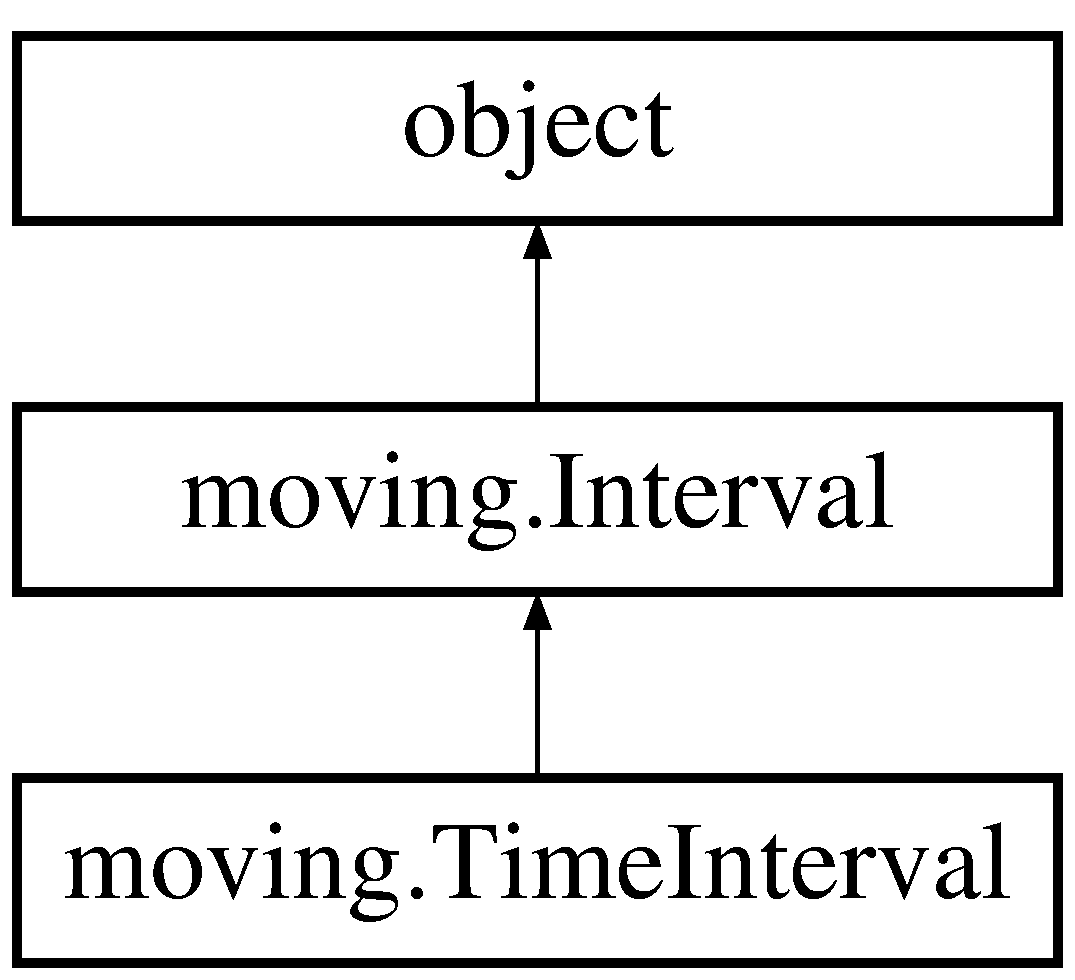
\includegraphics[height=3.000000cm]{classmoving_1_1Interval}
\end{center}
\end{figure}
\subsubsection*{Public Member Functions}
\begin{DoxyCompactItemize}
\item 
def \hyperlink{classmoving_1_1Interval_aa5eb3a435630c3c49b7c9a82a4d94b2d}{\-\_\-\-\_\-init\-\_\-\-\_\-}
\item 
def \hyperlink{classmoving_1_1Interval_ae25c61fee4181e5f514f697d6c5e48cf}{\-\_\-\-\_\-str\-\_\-\-\_\-}
\item 
def \hyperlink{classmoving_1_1Interval_ab04a2196fce936523edb9623b8f9dbb3}{\-\_\-\-\_\-repr\-\_\-\-\_\-}
\item 
def \hyperlink{classmoving_1_1Interval_a8c36083e8be78a79dda30c61fba71345}{empty}
\item 
def \hyperlink{classmoving_1_1Interval_a8cb325bee4428566f60d2c8b5e05962b}{center}
\item 
def \hyperlink{classmoving_1_1Interval_a757517d0850d1d93f9d04feb67c8797e}{length}
\item 
def \hyperlink{classmoving_1_1Interval_a021a0fb3910059e791e7ff9b277c2fca}{equal}
\item 
def \hyperlink{classmoving_1_1Interval_af8f41fb993da99a0a0a0a98d9b61a837}{get\-List}
\item 
def \hyperlink{classmoving_1_1Interval_adc454efd28e4ed275e1797d91708e550}{contains}
\item 
def \hyperlink{classmoving_1_1Interval_a46b32c9b16d430d6ae8e4b306cf1d2de}{inside}
\item 
def \hyperlink{classmoving_1_1Interval_ac7d8fca6600e97f5c342b957cfe82aec}{union}
\item 
def \hyperlink{classmoving_1_1Interval_a7cec40b2bf70166639d360d8fda3d20c}{intersection}
\item 
def \hyperlink{classmoving_1_1Interval_a17fab283bc671da2484217c5b4ed34e8}{distance}
\item 
def \hyperlink{classmoving_1_1Interval_a810cd43a545f5ca08edbc20643eebe84}{union\-Intervals}
\end{DoxyCompactItemize}
\subsubsection*{Public Attributes}
\begin{DoxyCompactItemize}
\item 
\hyperlink{classmoving_1_1Interval_a5f94e406b81e9461fb70a42f1cb6fbd7}{first}
\item 
\hyperlink{classmoving_1_1Interval_ac7a6353d124e726aa8a9a6b584ca07f5}{last}
\end{DoxyCompactItemize}


\subsubsection{Detailed Description}
\begin{DoxyVerb}Generic interval: a subset of real numbers (not iterable)\end{DoxyVerb}
 

\subsubsection{Constructor \& Destructor Documentation}
\hypertarget{classmoving_1_1Interval_aa5eb3a435630c3c49b7c9a82a4d94b2d}{\index{moving\-::\-Interval@{moving\-::\-Interval}!\-\_\-\-\_\-init\-\_\-\-\_\-@{\-\_\-\-\_\-init\-\_\-\-\_\-}}
\index{\-\_\-\-\_\-init\-\_\-\-\_\-@{\-\_\-\-\_\-init\-\_\-\-\_\-}!moving::Interval@{moving\-::\-Interval}}
\paragraph[{\-\_\-\-\_\-init\-\_\-\-\_\-}]{\setlength{\rightskip}{0pt plus 5cm}def moving.\-Interval.\-\_\-\-\_\-init\-\_\-\-\_\- (
\begin{DoxyParamCaption}
\item[{}]{self, }
\item[{}]{first = {\ttfamily 0}, }
\item[{}]{last = {\ttfamily -\/1}, }
\item[{}]{revert = {\ttfamily False}}
\end{DoxyParamCaption}
)}}\label{classmoving_1_1Interval_aa5eb3a435630c3c49b7c9a82a4d94b2d}


\subsubsection{Member Function Documentation}
\hypertarget{classmoving_1_1Interval_ab04a2196fce936523edb9623b8f9dbb3}{\index{moving\-::\-Interval@{moving\-::\-Interval}!\-\_\-\-\_\-repr\-\_\-\-\_\-@{\-\_\-\-\_\-repr\-\_\-\-\_\-}}
\index{\-\_\-\-\_\-repr\-\_\-\-\_\-@{\-\_\-\-\_\-repr\-\_\-\-\_\-}!moving::Interval@{moving\-::\-Interval}}
\paragraph[{\-\_\-\-\_\-repr\-\_\-\-\_\-}]{\setlength{\rightskip}{0pt plus 5cm}def moving.\-Interval.\-\_\-\-\_\-repr\-\_\-\-\_\- (
\begin{DoxyParamCaption}
\item[{}]{self}
\end{DoxyParamCaption}
)}}\label{classmoving_1_1Interval_ab04a2196fce936523edb9623b8f9dbb3}


References moving.\-Interval.\-\_\-\-\_\-str\-\_\-\-\_\-().

\hypertarget{classmoving_1_1Interval_ae25c61fee4181e5f514f697d6c5e48cf}{\index{moving\-::\-Interval@{moving\-::\-Interval}!\-\_\-\-\_\-str\-\_\-\-\_\-@{\-\_\-\-\_\-str\-\_\-\-\_\-}}
\index{\-\_\-\-\_\-str\-\_\-\-\_\-@{\-\_\-\-\_\-str\-\_\-\-\_\-}!moving::Interval@{moving\-::\-Interval}}
\paragraph[{\-\_\-\-\_\-str\-\_\-\-\_\-}]{\setlength{\rightskip}{0pt plus 5cm}def moving.\-Interval.\-\_\-\-\_\-str\-\_\-\-\_\- (
\begin{DoxyParamCaption}
\item[{}]{self}
\end{DoxyParamCaption}
)}}\label{classmoving_1_1Interval_ae25c61fee4181e5f514f697d6c5e48cf}


References moving.\-Interval.\-first, and moving.\-Interval.\-last.

\hypertarget{classmoving_1_1Interval_a8cb325bee4428566f60d2c8b5e05962b}{\index{moving\-::\-Interval@{moving\-::\-Interval}!center@{center}}
\index{center@{center}!moving::Interval@{moving\-::\-Interval}}
\paragraph[{center}]{\setlength{\rightskip}{0pt plus 5cm}def moving.\-Interval.\-center (
\begin{DoxyParamCaption}
\item[{}]{self}
\end{DoxyParamCaption}
)}}\label{classmoving_1_1Interval_a8cb325bee4428566f60d2c8b5e05962b}


References moving.\-Interval.\-first, and moving.\-Interval.\-last.

\hypertarget{classmoving_1_1Interval_adc454efd28e4ed275e1797d91708e550}{\index{moving\-::\-Interval@{moving\-::\-Interval}!contains@{contains}}
\index{contains@{contains}!moving::Interval@{moving\-::\-Interval}}
\paragraph[{contains}]{\setlength{\rightskip}{0pt plus 5cm}def moving.\-Interval.\-contains (
\begin{DoxyParamCaption}
\item[{}]{self, }
\item[{}]{instant}
\end{DoxyParamCaption}
)}}\label{classmoving_1_1Interval_adc454efd28e4ed275e1797d91708e550}


References moving.\-Interval.\-first, and moving.\-Interval.\-last.

\hypertarget{classmoving_1_1Interval_a17fab283bc671da2484217c5b4ed34e8}{\index{moving\-::\-Interval@{moving\-::\-Interval}!distance@{distance}}
\index{distance@{distance}!moving::Interval@{moving\-::\-Interval}}
\paragraph[{distance}]{\setlength{\rightskip}{0pt plus 5cm}def moving.\-Interval.\-distance (
\begin{DoxyParamCaption}
\item[{}]{self, }
\item[{}]{interval2}
\end{DoxyParamCaption}
)}}\label{classmoving_1_1Interval_a17fab283bc671da2484217c5b4ed34e8}


References moving.\-Interval.\-empty(), moving.\-Interval.\-first, and moving.\-Interval.\-last.

\hypertarget{classmoving_1_1Interval_a8c36083e8be78a79dda30c61fba71345}{\index{moving\-::\-Interval@{moving\-::\-Interval}!empty@{empty}}
\index{empty@{empty}!moving::Interval@{moving\-::\-Interval}}
\paragraph[{empty}]{\setlength{\rightskip}{0pt plus 5cm}def moving.\-Interval.\-empty (
\begin{DoxyParamCaption}
\item[{}]{self}
\end{DoxyParamCaption}
)}}\label{classmoving_1_1Interval_a8c36083e8be78a79dda30c61fba71345}


References moving.\-Interval.\-first, and moving.\-Interval.\-last.

\hypertarget{classmoving_1_1Interval_a021a0fb3910059e791e7ff9b277c2fca}{\index{moving\-::\-Interval@{moving\-::\-Interval}!equal@{equal}}
\index{equal@{equal}!moving::Interval@{moving\-::\-Interval}}
\paragraph[{equal}]{\setlength{\rightskip}{0pt plus 5cm}def moving.\-Interval.\-equal (
\begin{DoxyParamCaption}
\item[{}]{self, }
\item[{}]{i2}
\end{DoxyParamCaption}
)}}\label{classmoving_1_1Interval_a021a0fb3910059e791e7ff9b277c2fca}


References moving.\-Interval.\-first, and moving.\-Interval.\-last.

\hypertarget{classmoving_1_1Interval_af8f41fb993da99a0a0a0a98d9b61a837}{\index{moving\-::\-Interval@{moving\-::\-Interval}!get\-List@{get\-List}}
\index{get\-List@{get\-List}!moving::Interval@{moving\-::\-Interval}}
\paragraph[{get\-List}]{\setlength{\rightskip}{0pt plus 5cm}def moving.\-Interval.\-get\-List (
\begin{DoxyParamCaption}
\item[{}]{self}
\end{DoxyParamCaption}
)}}\label{classmoving_1_1Interval_af8f41fb993da99a0a0a0a98d9b61a837}


References moving.\-Interval.\-first, and moving.\-Interval.\-last.

\hypertarget{classmoving_1_1Interval_a46b32c9b16d430d6ae8e4b306cf1d2de}{\index{moving\-::\-Interval@{moving\-::\-Interval}!inside@{inside}}
\index{inside@{inside}!moving::Interval@{moving\-::\-Interval}}
\paragraph[{inside}]{\setlength{\rightskip}{0pt plus 5cm}def moving.\-Interval.\-inside (
\begin{DoxyParamCaption}
\item[{}]{self, }
\item[{}]{interval2}
\end{DoxyParamCaption}
)}}\label{classmoving_1_1Interval_a46b32c9b16d430d6ae8e4b306cf1d2de}
\begin{DoxyVerb}Indicates if the temporal interval of self is comprised in interval2\end{DoxyVerb}
 

References moving.\-Interval.\-first, and moving.\-Interval.\-last.

\hypertarget{classmoving_1_1Interval_a7cec40b2bf70166639d360d8fda3d20c}{\index{moving\-::\-Interval@{moving\-::\-Interval}!intersection@{intersection}}
\index{intersection@{intersection}!moving::Interval@{moving\-::\-Interval}}
\paragraph[{intersection}]{\setlength{\rightskip}{0pt plus 5cm}def moving.\-Interval.\-intersection (
\begin{DoxyParamCaption}
\item[{}]{cls, }
\item[{}]{interval1, }
\item[{}]{interval2}
\end{DoxyParamCaption}
)}}\label{classmoving_1_1Interval_a7cec40b2bf70166639d360d8fda3d20c}
\begin{DoxyVerb}Largest interval comprised in both self and interval2\end{DoxyVerb}
 \hypertarget{classmoving_1_1Interval_a757517d0850d1d93f9d04feb67c8797e}{\index{moving\-::\-Interval@{moving\-::\-Interval}!length@{length}}
\index{length@{length}!moving::Interval@{moving\-::\-Interval}}
\paragraph[{length}]{\setlength{\rightskip}{0pt plus 5cm}def moving.\-Interval.\-length (
\begin{DoxyParamCaption}
\item[{}]{self}
\end{DoxyParamCaption}
)}}\label{classmoving_1_1Interval_a757517d0850d1d93f9d04feb67c8797e}
\begin{DoxyVerb}Returns the length of the interval\end{DoxyVerb}
 

References moving.\-Interval.\-first, and moving.\-Interval.\-last.

\hypertarget{classmoving_1_1Interval_ac7d8fca6600e97f5c342b957cfe82aec}{\index{moving\-::\-Interval@{moving\-::\-Interval}!union@{union}}
\index{union@{union}!moving::Interval@{moving\-::\-Interval}}
\paragraph[{union}]{\setlength{\rightskip}{0pt plus 5cm}def moving.\-Interval.\-union (
\begin{DoxyParamCaption}
\item[{}]{cls, }
\item[{}]{interval1, }
\item[{}]{interval2}
\end{DoxyParamCaption}
)}}\label{classmoving_1_1Interval_ac7d8fca6600e97f5c342b957cfe82aec}
\begin{DoxyVerb}Smallest interval comprising self and interval2\end{DoxyVerb}
 \hypertarget{classmoving_1_1Interval_a810cd43a545f5ca08edbc20643eebe84}{\index{moving\-::\-Interval@{moving\-::\-Interval}!union\-Intervals@{union\-Intervals}}
\index{union\-Intervals@{union\-Intervals}!moving::Interval@{moving\-::\-Interval}}
\paragraph[{union\-Intervals}]{\setlength{\rightskip}{0pt plus 5cm}def moving.\-Interval.\-union\-Intervals (
\begin{DoxyParamCaption}
\item[{}]{cls, }
\item[{}]{intervals}
\end{DoxyParamCaption}
)}}\label{classmoving_1_1Interval_a810cd43a545f5ca08edbc20643eebe84}


\subsubsection{Member Data Documentation}
\hypertarget{classmoving_1_1Interval_a5f94e406b81e9461fb70a42f1cb6fbd7}{\index{moving\-::\-Interval@{moving\-::\-Interval}!first@{first}}
\index{first@{first}!moving::Interval@{moving\-::\-Interval}}
\paragraph[{first}]{\setlength{\rightskip}{0pt plus 5cm}moving.\-Interval.\-first}}\label{classmoving_1_1Interval_a5f94e406b81e9461fb70a42f1cb6fbd7}
\hypertarget{classmoving_1_1Interval_ac7a6353d124e726aa8a9a6b584ca07f5}{\index{moving\-::\-Interval@{moving\-::\-Interval}!last@{last}}
\index{last@{last}!moving::Interval@{moving\-::\-Interval}}
\paragraph[{last}]{\setlength{\rightskip}{0pt plus 5cm}moving.\-Interval.\-last}}\label{classmoving_1_1Interval_ac7a6353d124e726aa8a9a6b584ca07f5}


The documentation for this class was generated from the following file\-:\begin{DoxyCompactItemize}
\item 
python/\hyperlink{moving_8py}{moving.\-py}\end{DoxyCompactItemize}

\hypertarget{structCatch_1_1IReporter}{\subsection{Catch\-:\-:I\-Reporter Struct Reference}
\label{structCatch_1_1IReporter}\index{Catch\-::\-I\-Reporter@{Catch\-::\-I\-Reporter}}
}


{\ttfamily \#include $<$catch.\-hpp$>$}

Inheritance diagram for Catch\-:\-:I\-Reporter\-:\begin{figure}[H]
\begin{center}
\leavevmode
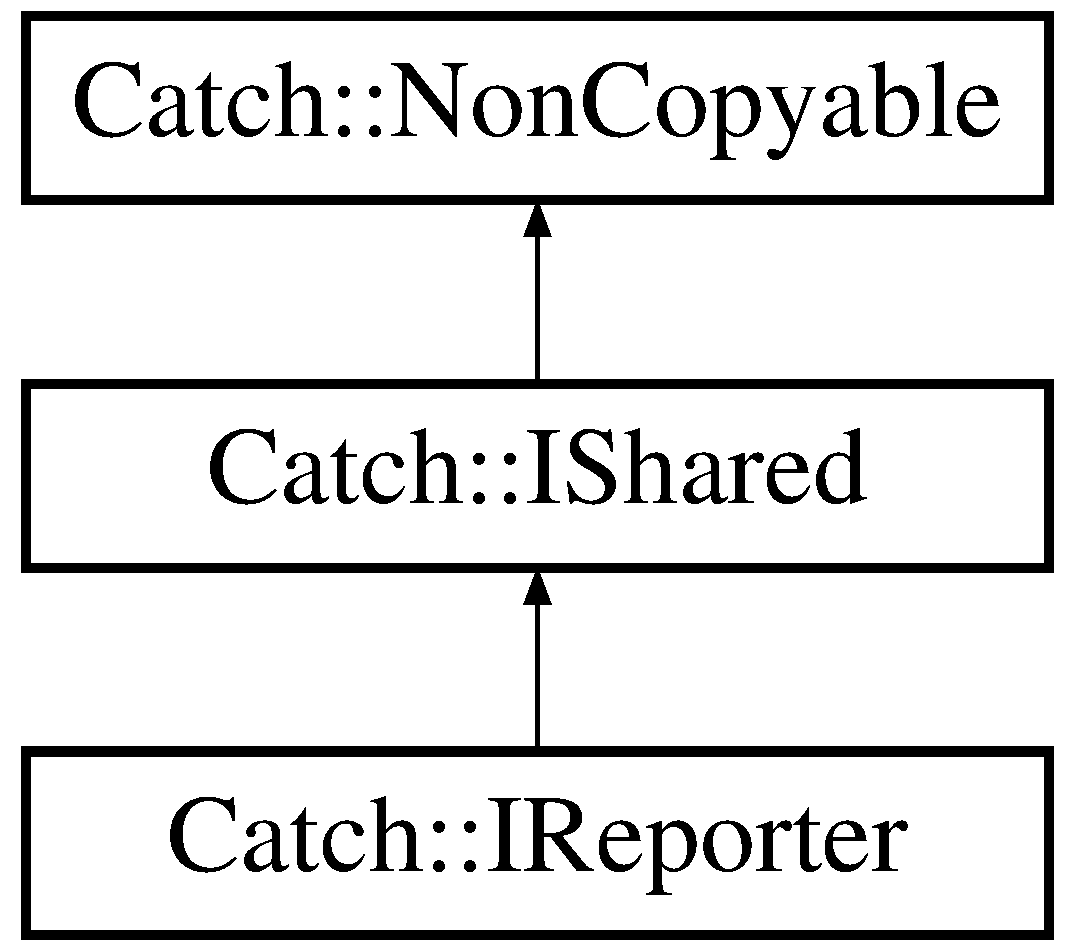
\includegraphics[height=3.000000cm]{structCatch_1_1IReporter}
\end{center}
\end{figure}
\subsubsection*{Public Member Functions}
\begin{DoxyCompactItemize}
\item 
virtual \hyperlink{structCatch_1_1IReporter_a0b9fdd30ff00c141af9df74821472c8c}{$\sim$\-I\-Reporter} ()
\item 
virtual bool \hyperlink{structCatch_1_1IReporter_aebd8c20478de29bba9b5a9f3845c18dc}{should\-Redirect\-Stdout} () const =0
\item 
virtual void \hyperlink{structCatch_1_1IReporter_afcf38d6ff912a9b2c7f07da45fcd5cb1}{Start\-Testing} ()=0
\item 
virtual void \hyperlink{structCatch_1_1IReporter_a26790d01ce89a9cededdea3de8dd2435}{End\-Testing} (const \hyperlink{structCatch_1_1Totals}{Totals} \&totals)=0
\item 
virtual void \hyperlink{structCatch_1_1IReporter_a376da40f5a20d5902393de93b367d70f}{Start\-Group} (const std\-::string \&group\-Name)=0
\item 
virtual void \hyperlink{structCatch_1_1IReporter_a4f535483a2b67ea035149bbb3cef329f}{End\-Group} (const std\-::string \&group\-Name, const \hyperlink{structCatch_1_1Totals}{Totals} \&totals)=0
\item 
virtual void \hyperlink{structCatch_1_1IReporter_adb0142a05b8fc99386a638515e2af388}{Start\-Section} (const std\-::string \&section\-Name, const std\-::string \&description)=0
\item 
virtual void \hyperlink{structCatch_1_1IReporter_a1d30e7c58ff3de2ae04d1741c80a74b2}{End\-Section} (const std\-::string \&section\-Name, const \hyperlink{structCatch_1_1Counts}{Counts} \&assertions)=0
\item 
virtual void \hyperlink{structCatch_1_1IReporter_a7951546119b0873f2f81cdaa61f3c60f}{Start\-Test\-Case} (const \hyperlink{classCatch_1_1TestCaseInfo}{Test\-Case\-Info} \&test\-Info)=0
\item 
virtual void \hyperlink{structCatch_1_1IReporter_a00d9d8bedcf32e5fdeed12b620b7ff7e}{Aborted} ()=0
\item 
virtual void \hyperlink{structCatch_1_1IReporter_a294e878c40061753eda12e326db31ec8}{End\-Test\-Case} (const \hyperlink{classCatch_1_1TestCaseInfo}{Test\-Case\-Info} \&test\-Info, const \hyperlink{structCatch_1_1Totals}{Totals} \&totals, const std\-::string \&std\-Out, const std\-::string \&std\-Err)=0
\item 
virtual void \hyperlink{structCatch_1_1IReporter_af3b99aa32bc7f92e3d6bf1e04ec1a5ee}{Result} (const \hyperlink{classCatch_1_1ResultInfo}{Result\-Info} \&result)=0
\end{DoxyCompactItemize}
\subsubsection*{Additional Inherited Members}


\subsubsection{Constructor \& Destructor Documentation}
\hypertarget{structCatch_1_1IReporter_a0b9fdd30ff00c141af9df74821472c8c}{\index{Catch\-::\-I\-Reporter@{Catch\-::\-I\-Reporter}!$\sim$\-I\-Reporter@{$\sim$\-I\-Reporter}}
\index{$\sim$\-I\-Reporter@{$\sim$\-I\-Reporter}!Catch::IReporter@{Catch\-::\-I\-Reporter}}
\paragraph[{$\sim$\-I\-Reporter}]{\setlength{\rightskip}{0pt plus 5cm}virtual Catch\-::\-I\-Reporter\-::$\sim$\-I\-Reporter (
\begin{DoxyParamCaption}
{}
\end{DoxyParamCaption}
)\hspace{0.3cm}{\ttfamily [inline]}, {\ttfamily [virtual]}}}\label{structCatch_1_1IReporter_a0b9fdd30ff00c141af9df74821472c8c}


\subsubsection{Member Function Documentation}
\hypertarget{structCatch_1_1IReporter_a00d9d8bedcf32e5fdeed12b620b7ff7e}{\index{Catch\-::\-I\-Reporter@{Catch\-::\-I\-Reporter}!Aborted@{Aborted}}
\index{Aborted@{Aborted}!Catch::IReporter@{Catch\-::\-I\-Reporter}}
\paragraph[{Aborted}]{\setlength{\rightskip}{0pt plus 5cm}virtual void Catch\-::\-I\-Reporter\-::\-Aborted (
\begin{DoxyParamCaption}
{}
\end{DoxyParamCaption}
)\hspace{0.3cm}{\ttfamily [pure virtual]}}}\label{structCatch_1_1IReporter_a00d9d8bedcf32e5fdeed12b620b7ff7e}
\hypertarget{structCatch_1_1IReporter_a4f535483a2b67ea035149bbb3cef329f}{\index{Catch\-::\-I\-Reporter@{Catch\-::\-I\-Reporter}!End\-Group@{End\-Group}}
\index{End\-Group@{End\-Group}!Catch::IReporter@{Catch\-::\-I\-Reporter}}
\paragraph[{End\-Group}]{\setlength{\rightskip}{0pt plus 5cm}virtual void Catch\-::\-I\-Reporter\-::\-End\-Group (
\begin{DoxyParamCaption}
\item[{const std\-::string \&}]{group\-Name, }
\item[{const {\bf Totals} \&}]{totals}
\end{DoxyParamCaption}
)\hspace{0.3cm}{\ttfamily [pure virtual]}}}\label{structCatch_1_1IReporter_a4f535483a2b67ea035149bbb3cef329f}
\hypertarget{structCatch_1_1IReporter_a1d30e7c58ff3de2ae04d1741c80a74b2}{\index{Catch\-::\-I\-Reporter@{Catch\-::\-I\-Reporter}!End\-Section@{End\-Section}}
\index{End\-Section@{End\-Section}!Catch::IReporter@{Catch\-::\-I\-Reporter}}
\paragraph[{End\-Section}]{\setlength{\rightskip}{0pt plus 5cm}virtual void Catch\-::\-I\-Reporter\-::\-End\-Section (
\begin{DoxyParamCaption}
\item[{const std\-::string \&}]{section\-Name, }
\item[{const {\bf Counts} \&}]{assertions}
\end{DoxyParamCaption}
)\hspace{0.3cm}{\ttfamily [pure virtual]}}}\label{structCatch_1_1IReporter_a1d30e7c58ff3de2ae04d1741c80a74b2}
\hypertarget{structCatch_1_1IReporter_a294e878c40061753eda12e326db31ec8}{\index{Catch\-::\-I\-Reporter@{Catch\-::\-I\-Reporter}!End\-Test\-Case@{End\-Test\-Case}}
\index{End\-Test\-Case@{End\-Test\-Case}!Catch::IReporter@{Catch\-::\-I\-Reporter}}
\paragraph[{End\-Test\-Case}]{\setlength{\rightskip}{0pt plus 5cm}virtual void Catch\-::\-I\-Reporter\-::\-End\-Test\-Case (
\begin{DoxyParamCaption}
\item[{const {\bf Test\-Case\-Info} \&}]{test\-Info, }
\item[{const {\bf Totals} \&}]{totals, }
\item[{const std\-::string \&}]{std\-Out, }
\item[{const std\-::string \&}]{std\-Err}
\end{DoxyParamCaption}
)\hspace{0.3cm}{\ttfamily [pure virtual]}}}\label{structCatch_1_1IReporter_a294e878c40061753eda12e326db31ec8}
\hypertarget{structCatch_1_1IReporter_a26790d01ce89a9cededdea3de8dd2435}{\index{Catch\-::\-I\-Reporter@{Catch\-::\-I\-Reporter}!End\-Testing@{End\-Testing}}
\index{End\-Testing@{End\-Testing}!Catch::IReporter@{Catch\-::\-I\-Reporter}}
\paragraph[{End\-Testing}]{\setlength{\rightskip}{0pt plus 5cm}virtual void Catch\-::\-I\-Reporter\-::\-End\-Testing (
\begin{DoxyParamCaption}
\item[{const {\bf Totals} \&}]{totals}
\end{DoxyParamCaption}
)\hspace{0.3cm}{\ttfamily [pure virtual]}}}\label{structCatch_1_1IReporter_a26790d01ce89a9cededdea3de8dd2435}
\hypertarget{structCatch_1_1IReporter_af3b99aa32bc7f92e3d6bf1e04ec1a5ee}{\index{Catch\-::\-I\-Reporter@{Catch\-::\-I\-Reporter}!Result@{Result}}
\index{Result@{Result}!Catch::IReporter@{Catch\-::\-I\-Reporter}}
\paragraph[{Result}]{\setlength{\rightskip}{0pt plus 5cm}virtual void Catch\-::\-I\-Reporter\-::\-Result (
\begin{DoxyParamCaption}
\item[{const {\bf Result\-Info} \&}]{result}
\end{DoxyParamCaption}
)\hspace{0.3cm}{\ttfamily [pure virtual]}}}\label{structCatch_1_1IReporter_af3b99aa32bc7f92e3d6bf1e04ec1a5ee}
\hypertarget{structCatch_1_1IReporter_aebd8c20478de29bba9b5a9f3845c18dc}{\index{Catch\-::\-I\-Reporter@{Catch\-::\-I\-Reporter}!should\-Redirect\-Stdout@{should\-Redirect\-Stdout}}
\index{should\-Redirect\-Stdout@{should\-Redirect\-Stdout}!Catch::IReporter@{Catch\-::\-I\-Reporter}}
\paragraph[{should\-Redirect\-Stdout}]{\setlength{\rightskip}{0pt plus 5cm}virtual bool Catch\-::\-I\-Reporter\-::should\-Redirect\-Stdout (
\begin{DoxyParamCaption}
{}
\end{DoxyParamCaption}
) const\hspace{0.3cm}{\ttfamily [pure virtual]}}}\label{structCatch_1_1IReporter_aebd8c20478de29bba9b5a9f3845c18dc}
\hypertarget{structCatch_1_1IReporter_a376da40f5a20d5902393de93b367d70f}{\index{Catch\-::\-I\-Reporter@{Catch\-::\-I\-Reporter}!Start\-Group@{Start\-Group}}
\index{Start\-Group@{Start\-Group}!Catch::IReporter@{Catch\-::\-I\-Reporter}}
\paragraph[{Start\-Group}]{\setlength{\rightskip}{0pt plus 5cm}virtual void Catch\-::\-I\-Reporter\-::\-Start\-Group (
\begin{DoxyParamCaption}
\item[{const std\-::string \&}]{group\-Name}
\end{DoxyParamCaption}
)\hspace{0.3cm}{\ttfamily [pure virtual]}}}\label{structCatch_1_1IReporter_a376da40f5a20d5902393de93b367d70f}
\hypertarget{structCatch_1_1IReporter_adb0142a05b8fc99386a638515e2af388}{\index{Catch\-::\-I\-Reporter@{Catch\-::\-I\-Reporter}!Start\-Section@{Start\-Section}}
\index{Start\-Section@{Start\-Section}!Catch::IReporter@{Catch\-::\-I\-Reporter}}
\paragraph[{Start\-Section}]{\setlength{\rightskip}{0pt plus 5cm}virtual void Catch\-::\-I\-Reporter\-::\-Start\-Section (
\begin{DoxyParamCaption}
\item[{const std\-::string \&}]{section\-Name, }
\item[{const std\-::string \&}]{description}
\end{DoxyParamCaption}
)\hspace{0.3cm}{\ttfamily [pure virtual]}}}\label{structCatch_1_1IReporter_adb0142a05b8fc99386a638515e2af388}
\hypertarget{structCatch_1_1IReporter_a7951546119b0873f2f81cdaa61f3c60f}{\index{Catch\-::\-I\-Reporter@{Catch\-::\-I\-Reporter}!Start\-Test\-Case@{Start\-Test\-Case}}
\index{Start\-Test\-Case@{Start\-Test\-Case}!Catch::IReporter@{Catch\-::\-I\-Reporter}}
\paragraph[{Start\-Test\-Case}]{\setlength{\rightskip}{0pt plus 5cm}virtual void Catch\-::\-I\-Reporter\-::\-Start\-Test\-Case (
\begin{DoxyParamCaption}
\item[{const {\bf Test\-Case\-Info} \&}]{test\-Info}
\end{DoxyParamCaption}
)\hspace{0.3cm}{\ttfamily [pure virtual]}}}\label{structCatch_1_1IReporter_a7951546119b0873f2f81cdaa61f3c60f}
\hypertarget{structCatch_1_1IReporter_afcf38d6ff912a9b2c7f07da45fcd5cb1}{\index{Catch\-::\-I\-Reporter@{Catch\-::\-I\-Reporter}!Start\-Testing@{Start\-Testing}}
\index{Start\-Testing@{Start\-Testing}!Catch::IReporter@{Catch\-::\-I\-Reporter}}
\paragraph[{Start\-Testing}]{\setlength{\rightskip}{0pt plus 5cm}virtual void Catch\-::\-I\-Reporter\-::\-Start\-Testing (
\begin{DoxyParamCaption}
{}
\end{DoxyParamCaption}
)\hspace{0.3cm}{\ttfamily [pure virtual]}}}\label{structCatch_1_1IReporter_afcf38d6ff912a9b2c7f07da45fcd5cb1}


The documentation for this struct was generated from the following file\-:\begin{DoxyCompactItemize}
\item 
include/\hyperlink{catch_8hpp}{catch.\-hpp}\end{DoxyCompactItemize}

\hypertarget{structCatch_1_1IReporterConfig}{\subsection{Catch\-:\-:I\-Reporter\-Config Struct Reference}
\label{structCatch_1_1IReporterConfig}\index{Catch\-::\-I\-Reporter\-Config@{Catch\-::\-I\-Reporter\-Config}}
}


{\ttfamily \#include $<$catch.\-hpp$>$}

\subsubsection*{Public Member Functions}
\begin{DoxyCompactItemize}
\item 
virtual \hyperlink{structCatch_1_1IReporterConfig_ae27ed8e89df244ca9accf4eeb1fdf041}{$\sim$\-I\-Reporter\-Config} ()
\item 
virtual std\-::ostream \& \hyperlink{structCatch_1_1IReporterConfig_a9844210e796c23c31dfd3cc0b30403c7}{stream} () const =0
\item 
virtual bool \hyperlink{structCatch_1_1IReporterConfig_a68e163202728c297f5873f98368ec403}{include\-Successful\-Results} () const =0
\item 
virtual std\-::string \hyperlink{structCatch_1_1IReporterConfig_a7dcef0d75fb00f8c5913652d0125f9e0}{get\-Name} () const =0
\end{DoxyCompactItemize}


\subsubsection{Constructor \& Destructor Documentation}
\hypertarget{structCatch_1_1IReporterConfig_ae27ed8e89df244ca9accf4eeb1fdf041}{\index{Catch\-::\-I\-Reporter\-Config@{Catch\-::\-I\-Reporter\-Config}!$\sim$\-I\-Reporter\-Config@{$\sim$\-I\-Reporter\-Config}}
\index{$\sim$\-I\-Reporter\-Config@{$\sim$\-I\-Reporter\-Config}!Catch::IReporterConfig@{Catch\-::\-I\-Reporter\-Config}}
\paragraph[{$\sim$\-I\-Reporter\-Config}]{\setlength{\rightskip}{0pt plus 5cm}virtual Catch\-::\-I\-Reporter\-Config\-::$\sim$\-I\-Reporter\-Config (
\begin{DoxyParamCaption}
{}
\end{DoxyParamCaption}
)\hspace{0.3cm}{\ttfamily [inline]}, {\ttfamily [virtual]}}}\label{structCatch_1_1IReporterConfig_ae27ed8e89df244ca9accf4eeb1fdf041}


\subsubsection{Member Function Documentation}
\hypertarget{structCatch_1_1IReporterConfig_a7dcef0d75fb00f8c5913652d0125f9e0}{\index{Catch\-::\-I\-Reporter\-Config@{Catch\-::\-I\-Reporter\-Config}!get\-Name@{get\-Name}}
\index{get\-Name@{get\-Name}!Catch::IReporterConfig@{Catch\-::\-I\-Reporter\-Config}}
\paragraph[{get\-Name}]{\setlength{\rightskip}{0pt plus 5cm}virtual std\-::string Catch\-::\-I\-Reporter\-Config\-::get\-Name (
\begin{DoxyParamCaption}
{}
\end{DoxyParamCaption}
) const\hspace{0.3cm}{\ttfamily [pure virtual]}}}\label{structCatch_1_1IReporterConfig_a7dcef0d75fb00f8c5913652d0125f9e0}
\hypertarget{structCatch_1_1IReporterConfig_a68e163202728c297f5873f98368ec403}{\index{Catch\-::\-I\-Reporter\-Config@{Catch\-::\-I\-Reporter\-Config}!include\-Successful\-Results@{include\-Successful\-Results}}
\index{include\-Successful\-Results@{include\-Successful\-Results}!Catch::IReporterConfig@{Catch\-::\-I\-Reporter\-Config}}
\paragraph[{include\-Successful\-Results}]{\setlength{\rightskip}{0pt plus 5cm}virtual bool Catch\-::\-I\-Reporter\-Config\-::include\-Successful\-Results (
\begin{DoxyParamCaption}
{}
\end{DoxyParamCaption}
) const\hspace{0.3cm}{\ttfamily [pure virtual]}}}\label{structCatch_1_1IReporterConfig_a68e163202728c297f5873f98368ec403}
\hypertarget{structCatch_1_1IReporterConfig_a9844210e796c23c31dfd3cc0b30403c7}{\index{Catch\-::\-I\-Reporter\-Config@{Catch\-::\-I\-Reporter\-Config}!stream@{stream}}
\index{stream@{stream}!Catch::IReporterConfig@{Catch\-::\-I\-Reporter\-Config}}
\paragraph[{stream}]{\setlength{\rightskip}{0pt plus 5cm}virtual std\-::ostream\& Catch\-::\-I\-Reporter\-Config\-::stream (
\begin{DoxyParamCaption}
{}
\end{DoxyParamCaption}
) const\hspace{0.3cm}{\ttfamily [pure virtual]}}}\label{structCatch_1_1IReporterConfig_a9844210e796c23c31dfd3cc0b30403c7}


The documentation for this struct was generated from the following file\-:\begin{DoxyCompactItemize}
\item 
include/\hyperlink{catch_8hpp}{catch.\-hpp}\end{DoxyCompactItemize}

\hypertarget{structCatch_1_1IReporterFactory}{\subsection{Catch\-:\-:I\-Reporter\-Factory Struct Reference}
\label{structCatch_1_1IReporterFactory}\index{Catch\-::\-I\-Reporter\-Factory@{Catch\-::\-I\-Reporter\-Factory}}
}


{\ttfamily \#include $<$catch.\-hpp$>$}

\subsubsection*{Public Member Functions}
\begin{DoxyCompactItemize}
\item 
virtual \hyperlink{structCatch_1_1IReporterFactory_a4011d1759be3a3a34a6e0b8bfbe8431c}{$\sim$\-I\-Reporter\-Factory} ()
\item 
virtual \hyperlink{structCatch_1_1IReporter}{I\-Reporter} $\ast$ \hyperlink{structCatch_1_1IReporterFactory_a91454578c249181e8c999060292a5f1e}{create} (const \hyperlink{structCatch_1_1IReporterConfig}{I\-Reporter\-Config} \&config) const =0
\item 
virtual std\-::string \hyperlink{structCatch_1_1IReporterFactory_a46880f93bd351d113d8189421928531b}{get\-Description} () const =0
\end{DoxyCompactItemize}


\subsubsection{Constructor \& Destructor Documentation}
\hypertarget{structCatch_1_1IReporterFactory_a4011d1759be3a3a34a6e0b8bfbe8431c}{\index{Catch\-::\-I\-Reporter\-Factory@{Catch\-::\-I\-Reporter\-Factory}!$\sim$\-I\-Reporter\-Factory@{$\sim$\-I\-Reporter\-Factory}}
\index{$\sim$\-I\-Reporter\-Factory@{$\sim$\-I\-Reporter\-Factory}!Catch::IReporterFactory@{Catch\-::\-I\-Reporter\-Factory}}
\paragraph[{$\sim$\-I\-Reporter\-Factory}]{\setlength{\rightskip}{0pt plus 5cm}virtual Catch\-::\-I\-Reporter\-Factory\-::$\sim$\-I\-Reporter\-Factory (
\begin{DoxyParamCaption}
{}
\end{DoxyParamCaption}
)\hspace{0.3cm}{\ttfamily [inline]}, {\ttfamily [virtual]}}}\label{structCatch_1_1IReporterFactory_a4011d1759be3a3a34a6e0b8bfbe8431c}


\subsubsection{Member Function Documentation}
\hypertarget{structCatch_1_1IReporterFactory_a91454578c249181e8c999060292a5f1e}{\index{Catch\-::\-I\-Reporter\-Factory@{Catch\-::\-I\-Reporter\-Factory}!create@{create}}
\index{create@{create}!Catch::IReporterFactory@{Catch\-::\-I\-Reporter\-Factory}}
\paragraph[{create}]{\setlength{\rightskip}{0pt plus 5cm}virtual {\bf I\-Reporter}$\ast$ Catch\-::\-I\-Reporter\-Factory\-::create (
\begin{DoxyParamCaption}
\item[{const {\bf I\-Reporter\-Config} \&}]{config}
\end{DoxyParamCaption}
) const\hspace{0.3cm}{\ttfamily [pure virtual]}}}\label{structCatch_1_1IReporterFactory_a91454578c249181e8c999060292a5f1e}
\hypertarget{structCatch_1_1IReporterFactory_a46880f93bd351d113d8189421928531b}{\index{Catch\-::\-I\-Reporter\-Factory@{Catch\-::\-I\-Reporter\-Factory}!get\-Description@{get\-Description}}
\index{get\-Description@{get\-Description}!Catch::IReporterFactory@{Catch\-::\-I\-Reporter\-Factory}}
\paragraph[{get\-Description}]{\setlength{\rightskip}{0pt plus 5cm}virtual std\-::string Catch\-::\-I\-Reporter\-Factory\-::get\-Description (
\begin{DoxyParamCaption}
{}
\end{DoxyParamCaption}
) const\hspace{0.3cm}{\ttfamily [pure virtual]}}}\label{structCatch_1_1IReporterFactory_a46880f93bd351d113d8189421928531b}


The documentation for this struct was generated from the following file\-:\begin{DoxyCompactItemize}
\item 
include/\hyperlink{catch_8hpp}{catch.\-hpp}\end{DoxyCompactItemize}

\hypertarget{structCatch_1_1IReporterRegistry}{\subsection{Catch\-:\-:I\-Reporter\-Registry Struct Reference}
\label{structCatch_1_1IReporterRegistry}\index{Catch\-::\-I\-Reporter\-Registry@{Catch\-::\-I\-Reporter\-Registry}}
}


{\ttfamily \#include $<$catch.\-hpp$>$}

\subsubsection*{Public Types}
\begin{DoxyCompactItemize}
\item 
typedef std\-::map$<$ std\-::string, \\*
\hyperlink{structCatch_1_1IReporterFactory}{I\-Reporter\-Factory} $\ast$ $>$ \hyperlink{structCatch_1_1IReporterRegistry_a328440adc2303a1e31bdc763f0504452}{Factory\-Map}
\end{DoxyCompactItemize}
\subsubsection*{Public Member Functions}
\begin{DoxyCompactItemize}
\item 
virtual \hyperlink{structCatch_1_1IReporterRegistry_a6f71b633176df8f005876e54db0b1ac9}{$\sim$\-I\-Reporter\-Registry} ()
\item 
virtual \hyperlink{structCatch_1_1IReporter}{I\-Reporter} $\ast$ \hyperlink{structCatch_1_1IReporterRegistry_a68525958fb5ce3aa3c7f974191a71686}{create} (const std\-::string \&name, const \hyperlink{structCatch_1_1IReporterConfig}{I\-Reporter\-Config} \&config) const =0
\item 
virtual void \hyperlink{structCatch_1_1IReporterRegistry_a9da0e7dbe81135536734962809e3cacf}{register\-Reporter} (const std\-::string \&name, \hyperlink{structCatch_1_1IReporterFactory}{I\-Reporter\-Factory} $\ast$factory)=0
\item 
virtual const \hyperlink{structCatch_1_1IReporterRegistry_a328440adc2303a1e31bdc763f0504452}{Factory\-Map} \& \hyperlink{structCatch_1_1IReporterRegistry_a8ee40835aa4a8c2810754f2074dec982}{get\-Factories} () const =0
\end{DoxyCompactItemize}


\subsubsection{Member Typedef Documentation}
\hypertarget{structCatch_1_1IReporterRegistry_a328440adc2303a1e31bdc763f0504452}{\index{Catch\-::\-I\-Reporter\-Registry@{Catch\-::\-I\-Reporter\-Registry}!Factory\-Map@{Factory\-Map}}
\index{Factory\-Map@{Factory\-Map}!Catch::IReporterRegistry@{Catch\-::\-I\-Reporter\-Registry}}
\paragraph[{Factory\-Map}]{\setlength{\rightskip}{0pt plus 5cm}typedef std\-::map$<$std\-::string, {\bf I\-Reporter\-Factory}$\ast$$>$ {\bf Catch\-::\-I\-Reporter\-Registry\-::\-Factory\-Map}}}\label{structCatch_1_1IReporterRegistry_a328440adc2303a1e31bdc763f0504452}


\subsubsection{Constructor \& Destructor Documentation}
\hypertarget{structCatch_1_1IReporterRegistry_a6f71b633176df8f005876e54db0b1ac9}{\index{Catch\-::\-I\-Reporter\-Registry@{Catch\-::\-I\-Reporter\-Registry}!$\sim$\-I\-Reporter\-Registry@{$\sim$\-I\-Reporter\-Registry}}
\index{$\sim$\-I\-Reporter\-Registry@{$\sim$\-I\-Reporter\-Registry}!Catch::IReporterRegistry@{Catch\-::\-I\-Reporter\-Registry}}
\paragraph[{$\sim$\-I\-Reporter\-Registry}]{\setlength{\rightskip}{0pt plus 5cm}virtual Catch\-::\-I\-Reporter\-Registry\-::$\sim$\-I\-Reporter\-Registry (
\begin{DoxyParamCaption}
{}
\end{DoxyParamCaption}
)\hspace{0.3cm}{\ttfamily [inline]}, {\ttfamily [virtual]}}}\label{structCatch_1_1IReporterRegistry_a6f71b633176df8f005876e54db0b1ac9}


\subsubsection{Member Function Documentation}
\hypertarget{structCatch_1_1IReporterRegistry_a68525958fb5ce3aa3c7f974191a71686}{\index{Catch\-::\-I\-Reporter\-Registry@{Catch\-::\-I\-Reporter\-Registry}!create@{create}}
\index{create@{create}!Catch::IReporterRegistry@{Catch\-::\-I\-Reporter\-Registry}}
\paragraph[{create}]{\setlength{\rightskip}{0pt plus 5cm}virtual {\bf I\-Reporter}$\ast$ Catch\-::\-I\-Reporter\-Registry\-::create (
\begin{DoxyParamCaption}
\item[{const std\-::string \&}]{name, }
\item[{const {\bf I\-Reporter\-Config} \&}]{config}
\end{DoxyParamCaption}
) const\hspace{0.3cm}{\ttfamily [pure virtual]}}}\label{structCatch_1_1IReporterRegistry_a68525958fb5ce3aa3c7f974191a71686}
\hypertarget{structCatch_1_1IReporterRegistry_a8ee40835aa4a8c2810754f2074dec982}{\index{Catch\-::\-I\-Reporter\-Registry@{Catch\-::\-I\-Reporter\-Registry}!get\-Factories@{get\-Factories}}
\index{get\-Factories@{get\-Factories}!Catch::IReporterRegistry@{Catch\-::\-I\-Reporter\-Registry}}
\paragraph[{get\-Factories}]{\setlength{\rightskip}{0pt plus 5cm}virtual const {\bf Factory\-Map}\& Catch\-::\-I\-Reporter\-Registry\-::get\-Factories (
\begin{DoxyParamCaption}
{}
\end{DoxyParamCaption}
) const\hspace{0.3cm}{\ttfamily [pure virtual]}}}\label{structCatch_1_1IReporterRegistry_a8ee40835aa4a8c2810754f2074dec982}
\hypertarget{structCatch_1_1IReporterRegistry_a9da0e7dbe81135536734962809e3cacf}{\index{Catch\-::\-I\-Reporter\-Registry@{Catch\-::\-I\-Reporter\-Registry}!register\-Reporter@{register\-Reporter}}
\index{register\-Reporter@{register\-Reporter}!Catch::IReporterRegistry@{Catch\-::\-I\-Reporter\-Registry}}
\paragraph[{register\-Reporter}]{\setlength{\rightskip}{0pt plus 5cm}virtual void Catch\-::\-I\-Reporter\-Registry\-::register\-Reporter (
\begin{DoxyParamCaption}
\item[{const std\-::string \&}]{name, }
\item[{{\bf I\-Reporter\-Factory} $\ast$}]{factory}
\end{DoxyParamCaption}
)\hspace{0.3cm}{\ttfamily [pure virtual]}}}\label{structCatch_1_1IReporterRegistry_a9da0e7dbe81135536734962809e3cacf}


The documentation for this struct was generated from the following file\-:\begin{DoxyCompactItemize}
\item 
include/\hyperlink{catch_8hpp}{catch.\-hpp}\end{DoxyCompactItemize}

\hypertarget{structCatch_1_1IResultCapture}{\subsection{Catch\-:\-:I\-Result\-Capture Struct Reference}
\label{structCatch_1_1IResultCapture}\index{Catch\-::\-I\-Result\-Capture@{Catch\-::\-I\-Result\-Capture}}
}


{\ttfamily \#include $<$catch.\-hpp$>$}

\subsubsection*{Public Member Functions}
\begin{DoxyCompactItemize}
\item 
virtual \hyperlink{structCatch_1_1IResultCapture_a3bd16719d6772b7470887fc36c6d0808}{$\sim$\-I\-Result\-Capture} ()
\item 
virtual void \hyperlink{structCatch_1_1IResultCapture_a3a17532fc7d18e78b83f3d31e93b9217}{test\-Ended} (const \hyperlink{classCatch_1_1ResultInfo}{Result\-Info} \&result)=0
\item 
virtual bool \hyperlink{structCatch_1_1IResultCapture_af6334f4c1aa674d22c7f1054a82dbf16}{section\-Started} (const std\-::string \&name, const std\-::string \&description, const \hyperlink{structCatch_1_1SourceLineInfo}{Source\-Line\-Info} \&line\-Info, \hyperlink{structCatch_1_1Counts}{Counts} \&assertions)=0
\item 
virtual void \hyperlink{structCatch_1_1IResultCapture_add91031c212d37bcc5aadf9bdccb9319}{section\-Ended} (const std\-::string \&name, const \hyperlink{structCatch_1_1Counts}{Counts} \&assertions)=0
\item 
virtual void \hyperlink{structCatch_1_1IResultCapture_a372979aab5e851cfafceff905d6493a7}{push\-Scoped\-Info} (\hyperlink{classCatch_1_1ScopedInfo}{Scoped\-Info} $\ast$scoped\-Info)=0
\item 
virtual void \hyperlink{structCatch_1_1IResultCapture_a8d6fd1ef854284b77c35a44b3e1b5929}{pop\-Scoped\-Info} (\hyperlink{classCatch_1_1ScopedInfo}{Scoped\-Info} $\ast$scoped\-Info)=0
\item 
virtual bool \hyperlink{structCatch_1_1IResultCapture_a7839e422ccd55f298cd64f0bf4a5938b}{should\-Debug\-Break} () const =0
\item 
virtual \hyperlink{structCatch_1_1ResultAction_a42d1644a0fbcedc17959b656ce68f88d}{Result\-Action\-::\-Value} \hyperlink{structCatch_1_1IResultCapture_a9701dc69864613d6982239f2ddc358c5}{accept\-Result} (bool result)=0
\item 
virtual \hyperlink{structCatch_1_1ResultAction_a42d1644a0fbcedc17959b656ce68f88d}{Result\-Action\-::\-Value} \hyperlink{structCatch_1_1IResultCapture_a24589cc2ad478b2e9f27264a3c5a422e}{accept\-Result} (\hyperlink{structCatch_1_1ResultWas_a624e1ee3661fcf6094ceef1f654601ef}{Result\-Was\-::\-Of\-Type} result)=0
\item 
virtual \hyperlink{structCatch_1_1ResultAction_a42d1644a0fbcedc17959b656ce68f88d}{Result\-Action\-::\-Value} \hyperlink{structCatch_1_1IResultCapture_aa8bb54e8173ba43ae5fbbb7c9c227384}{accept\-Expression} (const \hyperlink{classCatch_1_1ResultInfoBuilder}{Result\-Info\-Builder} \&result\-Info)=0
\item 
virtual void \hyperlink{structCatch_1_1IResultCapture_a8ca9f56738b5c3b2cf30fb3bdb56dd7b}{accept\-Message} (const std\-::string \&msg)=0
\item 
virtual std\-::string \hyperlink{structCatch_1_1IResultCapture_aea1617f4a84cc648246aa3ed6918b5bf}{get\-Current\-Test\-Name} () const =0
\item 
virtual const \hyperlink{classCatch_1_1ResultInfo}{Result\-Info} $\ast$ \hyperlink{structCatch_1_1IResultCapture_a1b3185be3a5a1e48b8038a910245d6e7}{get\-Last\-Result} () const =0
\end{DoxyCompactItemize}


\subsubsection{Constructor \& Destructor Documentation}
\hypertarget{structCatch_1_1IResultCapture_a3bd16719d6772b7470887fc36c6d0808}{\index{Catch\-::\-I\-Result\-Capture@{Catch\-::\-I\-Result\-Capture}!$\sim$\-I\-Result\-Capture@{$\sim$\-I\-Result\-Capture}}
\index{$\sim$\-I\-Result\-Capture@{$\sim$\-I\-Result\-Capture}!Catch::IResultCapture@{Catch\-::\-I\-Result\-Capture}}
\paragraph[{$\sim$\-I\-Result\-Capture}]{\setlength{\rightskip}{0pt plus 5cm}virtual Catch\-::\-I\-Result\-Capture\-::$\sim$\-I\-Result\-Capture (
\begin{DoxyParamCaption}
{}
\end{DoxyParamCaption}
)\hspace{0.3cm}{\ttfamily [inline]}, {\ttfamily [virtual]}}}\label{structCatch_1_1IResultCapture_a3bd16719d6772b7470887fc36c6d0808}


\subsubsection{Member Function Documentation}
\hypertarget{structCatch_1_1IResultCapture_aa8bb54e8173ba43ae5fbbb7c9c227384}{\index{Catch\-::\-I\-Result\-Capture@{Catch\-::\-I\-Result\-Capture}!accept\-Expression@{accept\-Expression}}
\index{accept\-Expression@{accept\-Expression}!Catch::IResultCapture@{Catch\-::\-I\-Result\-Capture}}
\paragraph[{accept\-Expression}]{\setlength{\rightskip}{0pt plus 5cm}virtual {\bf Result\-Action\-::\-Value} Catch\-::\-I\-Result\-Capture\-::accept\-Expression (
\begin{DoxyParamCaption}
\item[{const {\bf Result\-Info\-Builder} \&}]{result\-Info}
\end{DoxyParamCaption}
)\hspace{0.3cm}{\ttfamily [pure virtual]}}}\label{structCatch_1_1IResultCapture_aa8bb54e8173ba43ae5fbbb7c9c227384}
\hypertarget{structCatch_1_1IResultCapture_a8ca9f56738b5c3b2cf30fb3bdb56dd7b}{\index{Catch\-::\-I\-Result\-Capture@{Catch\-::\-I\-Result\-Capture}!accept\-Message@{accept\-Message}}
\index{accept\-Message@{accept\-Message}!Catch::IResultCapture@{Catch\-::\-I\-Result\-Capture}}
\paragraph[{accept\-Message}]{\setlength{\rightskip}{0pt plus 5cm}virtual void Catch\-::\-I\-Result\-Capture\-::accept\-Message (
\begin{DoxyParamCaption}
\item[{const std\-::string \&}]{msg}
\end{DoxyParamCaption}
)\hspace{0.3cm}{\ttfamily [pure virtual]}}}\label{structCatch_1_1IResultCapture_a8ca9f56738b5c3b2cf30fb3bdb56dd7b}
\hypertarget{structCatch_1_1IResultCapture_a9701dc69864613d6982239f2ddc358c5}{\index{Catch\-::\-I\-Result\-Capture@{Catch\-::\-I\-Result\-Capture}!accept\-Result@{accept\-Result}}
\index{accept\-Result@{accept\-Result}!Catch::IResultCapture@{Catch\-::\-I\-Result\-Capture}}
\paragraph[{accept\-Result}]{\setlength{\rightskip}{0pt plus 5cm}virtual {\bf Result\-Action\-::\-Value} Catch\-::\-I\-Result\-Capture\-::accept\-Result (
\begin{DoxyParamCaption}
\item[{bool}]{result}
\end{DoxyParamCaption}
)\hspace{0.3cm}{\ttfamily [pure virtual]}}}\label{structCatch_1_1IResultCapture_a9701dc69864613d6982239f2ddc358c5}
\hypertarget{structCatch_1_1IResultCapture_a24589cc2ad478b2e9f27264a3c5a422e}{\index{Catch\-::\-I\-Result\-Capture@{Catch\-::\-I\-Result\-Capture}!accept\-Result@{accept\-Result}}
\index{accept\-Result@{accept\-Result}!Catch::IResultCapture@{Catch\-::\-I\-Result\-Capture}}
\paragraph[{accept\-Result}]{\setlength{\rightskip}{0pt plus 5cm}virtual {\bf Result\-Action\-::\-Value} Catch\-::\-I\-Result\-Capture\-::accept\-Result (
\begin{DoxyParamCaption}
\item[{{\bf Result\-Was\-::\-Of\-Type}}]{result}
\end{DoxyParamCaption}
)\hspace{0.3cm}{\ttfamily [pure virtual]}}}\label{structCatch_1_1IResultCapture_a24589cc2ad478b2e9f27264a3c5a422e}
\hypertarget{structCatch_1_1IResultCapture_aea1617f4a84cc648246aa3ed6918b5bf}{\index{Catch\-::\-I\-Result\-Capture@{Catch\-::\-I\-Result\-Capture}!get\-Current\-Test\-Name@{get\-Current\-Test\-Name}}
\index{get\-Current\-Test\-Name@{get\-Current\-Test\-Name}!Catch::IResultCapture@{Catch\-::\-I\-Result\-Capture}}
\paragraph[{get\-Current\-Test\-Name}]{\setlength{\rightskip}{0pt plus 5cm}virtual std\-::string Catch\-::\-I\-Result\-Capture\-::get\-Current\-Test\-Name (
\begin{DoxyParamCaption}
{}
\end{DoxyParamCaption}
) const\hspace{0.3cm}{\ttfamily [pure virtual]}}}\label{structCatch_1_1IResultCapture_aea1617f4a84cc648246aa3ed6918b5bf}
\hypertarget{structCatch_1_1IResultCapture_a1b3185be3a5a1e48b8038a910245d6e7}{\index{Catch\-::\-I\-Result\-Capture@{Catch\-::\-I\-Result\-Capture}!get\-Last\-Result@{get\-Last\-Result}}
\index{get\-Last\-Result@{get\-Last\-Result}!Catch::IResultCapture@{Catch\-::\-I\-Result\-Capture}}
\paragraph[{get\-Last\-Result}]{\setlength{\rightskip}{0pt plus 5cm}virtual const {\bf Result\-Info}$\ast$ Catch\-::\-I\-Result\-Capture\-::get\-Last\-Result (
\begin{DoxyParamCaption}
{}
\end{DoxyParamCaption}
) const\hspace{0.3cm}{\ttfamily [pure virtual]}}}\label{structCatch_1_1IResultCapture_a1b3185be3a5a1e48b8038a910245d6e7}
\hypertarget{structCatch_1_1IResultCapture_a8d6fd1ef854284b77c35a44b3e1b5929}{\index{Catch\-::\-I\-Result\-Capture@{Catch\-::\-I\-Result\-Capture}!pop\-Scoped\-Info@{pop\-Scoped\-Info}}
\index{pop\-Scoped\-Info@{pop\-Scoped\-Info}!Catch::IResultCapture@{Catch\-::\-I\-Result\-Capture}}
\paragraph[{pop\-Scoped\-Info}]{\setlength{\rightskip}{0pt plus 5cm}virtual void Catch\-::\-I\-Result\-Capture\-::pop\-Scoped\-Info (
\begin{DoxyParamCaption}
\item[{{\bf Scoped\-Info} $\ast$}]{scoped\-Info}
\end{DoxyParamCaption}
)\hspace{0.3cm}{\ttfamily [pure virtual]}}}\label{structCatch_1_1IResultCapture_a8d6fd1ef854284b77c35a44b3e1b5929}
\hypertarget{structCatch_1_1IResultCapture_a372979aab5e851cfafceff905d6493a7}{\index{Catch\-::\-I\-Result\-Capture@{Catch\-::\-I\-Result\-Capture}!push\-Scoped\-Info@{push\-Scoped\-Info}}
\index{push\-Scoped\-Info@{push\-Scoped\-Info}!Catch::IResultCapture@{Catch\-::\-I\-Result\-Capture}}
\paragraph[{push\-Scoped\-Info}]{\setlength{\rightskip}{0pt plus 5cm}virtual void Catch\-::\-I\-Result\-Capture\-::push\-Scoped\-Info (
\begin{DoxyParamCaption}
\item[{{\bf Scoped\-Info} $\ast$}]{scoped\-Info}
\end{DoxyParamCaption}
)\hspace{0.3cm}{\ttfamily [pure virtual]}}}\label{structCatch_1_1IResultCapture_a372979aab5e851cfafceff905d6493a7}
\hypertarget{structCatch_1_1IResultCapture_add91031c212d37bcc5aadf9bdccb9319}{\index{Catch\-::\-I\-Result\-Capture@{Catch\-::\-I\-Result\-Capture}!section\-Ended@{section\-Ended}}
\index{section\-Ended@{section\-Ended}!Catch::IResultCapture@{Catch\-::\-I\-Result\-Capture}}
\paragraph[{section\-Ended}]{\setlength{\rightskip}{0pt plus 5cm}virtual void Catch\-::\-I\-Result\-Capture\-::section\-Ended (
\begin{DoxyParamCaption}
\item[{const std\-::string \&}]{name, }
\item[{const {\bf Counts} \&}]{assertions}
\end{DoxyParamCaption}
)\hspace{0.3cm}{\ttfamily [pure virtual]}}}\label{structCatch_1_1IResultCapture_add91031c212d37bcc5aadf9bdccb9319}
\hypertarget{structCatch_1_1IResultCapture_af6334f4c1aa674d22c7f1054a82dbf16}{\index{Catch\-::\-I\-Result\-Capture@{Catch\-::\-I\-Result\-Capture}!section\-Started@{section\-Started}}
\index{section\-Started@{section\-Started}!Catch::IResultCapture@{Catch\-::\-I\-Result\-Capture}}
\paragraph[{section\-Started}]{\setlength{\rightskip}{0pt plus 5cm}virtual bool Catch\-::\-I\-Result\-Capture\-::section\-Started (
\begin{DoxyParamCaption}
\item[{const std\-::string \&}]{name, }
\item[{const std\-::string \&}]{description, }
\item[{const {\bf Source\-Line\-Info} \&}]{line\-Info, }
\item[{{\bf Counts} \&}]{assertions}
\end{DoxyParamCaption}
)\hspace{0.3cm}{\ttfamily [pure virtual]}}}\label{structCatch_1_1IResultCapture_af6334f4c1aa674d22c7f1054a82dbf16}
\hypertarget{structCatch_1_1IResultCapture_a7839e422ccd55f298cd64f0bf4a5938b}{\index{Catch\-::\-I\-Result\-Capture@{Catch\-::\-I\-Result\-Capture}!should\-Debug\-Break@{should\-Debug\-Break}}
\index{should\-Debug\-Break@{should\-Debug\-Break}!Catch::IResultCapture@{Catch\-::\-I\-Result\-Capture}}
\paragraph[{should\-Debug\-Break}]{\setlength{\rightskip}{0pt plus 5cm}virtual bool Catch\-::\-I\-Result\-Capture\-::should\-Debug\-Break (
\begin{DoxyParamCaption}
{}
\end{DoxyParamCaption}
) const\hspace{0.3cm}{\ttfamily [pure virtual]}}}\label{structCatch_1_1IResultCapture_a7839e422ccd55f298cd64f0bf4a5938b}
\hypertarget{structCatch_1_1IResultCapture_a3a17532fc7d18e78b83f3d31e93b9217}{\index{Catch\-::\-I\-Result\-Capture@{Catch\-::\-I\-Result\-Capture}!test\-Ended@{test\-Ended}}
\index{test\-Ended@{test\-Ended}!Catch::IResultCapture@{Catch\-::\-I\-Result\-Capture}}
\paragraph[{test\-Ended}]{\setlength{\rightskip}{0pt plus 5cm}virtual void Catch\-::\-I\-Result\-Capture\-::test\-Ended (
\begin{DoxyParamCaption}
\item[{const {\bf Result\-Info} \&}]{result}
\end{DoxyParamCaption}
)\hspace{0.3cm}{\ttfamily [pure virtual]}}}\label{structCatch_1_1IResultCapture_a3a17532fc7d18e78b83f3d31e93b9217}


The documentation for this struct was generated from the following file\-:\begin{DoxyCompactItemize}
\item 
include/\hyperlink{catch_8hpp}{catch.\-hpp}\end{DoxyCompactItemize}

\hypertarget{structCatch_1_1IRunner}{\subsection{Catch\-:\-:I\-Runner Struct Reference}
\label{structCatch_1_1IRunner}\index{Catch\-::\-I\-Runner@{Catch\-::\-I\-Runner}}
}


{\ttfamily \#include $<$catch.\-hpp$>$}

\subsubsection*{Public Member Functions}
\begin{DoxyCompactItemize}
\item 
virtual \hyperlink{structCatch_1_1IRunner_a5f539a88a7772d68de8a2e4028774209}{$\sim$\-I\-Runner} ()
\item 
virtual void \hyperlink{structCatch_1_1IRunner_aa5d8b444dff60e05c3d812e7ad6bed14}{run\-All} (bool run\-Hidden\-Tests=false)=0
\item 
virtual std\-::size\-\_\-t \hyperlink{structCatch_1_1IRunner_aac809306e347bae6d152faf01e4af1fb}{run\-Matching} (const std\-::string \&raw\-Test\-Spec)=0
\item 
virtual \hyperlink{structCatch_1_1Totals}{Totals} \hyperlink{structCatch_1_1IRunner_a1ad5081c2ac06c27db6015a744ea2093}{get\-Totals} () const =0
\end{DoxyCompactItemize}


\subsubsection{Constructor \& Destructor Documentation}
\hypertarget{structCatch_1_1IRunner_a5f539a88a7772d68de8a2e4028774209}{\index{Catch\-::\-I\-Runner@{Catch\-::\-I\-Runner}!$\sim$\-I\-Runner@{$\sim$\-I\-Runner}}
\index{$\sim$\-I\-Runner@{$\sim$\-I\-Runner}!Catch::IRunner@{Catch\-::\-I\-Runner}}
\paragraph[{$\sim$\-I\-Runner}]{\setlength{\rightskip}{0pt plus 5cm}virtual Catch\-::\-I\-Runner\-::$\sim$\-I\-Runner (
\begin{DoxyParamCaption}
{}
\end{DoxyParamCaption}
)\hspace{0.3cm}{\ttfamily [inline]}, {\ttfamily [virtual]}}}\label{structCatch_1_1IRunner_a5f539a88a7772d68de8a2e4028774209}


\subsubsection{Member Function Documentation}
\hypertarget{structCatch_1_1IRunner_a1ad5081c2ac06c27db6015a744ea2093}{\index{Catch\-::\-I\-Runner@{Catch\-::\-I\-Runner}!get\-Totals@{get\-Totals}}
\index{get\-Totals@{get\-Totals}!Catch::IRunner@{Catch\-::\-I\-Runner}}
\paragraph[{get\-Totals}]{\setlength{\rightskip}{0pt plus 5cm}virtual {\bf Totals} Catch\-::\-I\-Runner\-::get\-Totals (
\begin{DoxyParamCaption}
{}
\end{DoxyParamCaption}
) const\hspace{0.3cm}{\ttfamily [pure virtual]}}}\label{structCatch_1_1IRunner_a1ad5081c2ac06c27db6015a744ea2093}
\hypertarget{structCatch_1_1IRunner_aa5d8b444dff60e05c3d812e7ad6bed14}{\index{Catch\-::\-I\-Runner@{Catch\-::\-I\-Runner}!run\-All@{run\-All}}
\index{run\-All@{run\-All}!Catch::IRunner@{Catch\-::\-I\-Runner}}
\paragraph[{run\-All}]{\setlength{\rightskip}{0pt plus 5cm}virtual void Catch\-::\-I\-Runner\-::run\-All (
\begin{DoxyParamCaption}
\item[{bool}]{run\-Hidden\-Tests = {\ttfamily false}}
\end{DoxyParamCaption}
)\hspace{0.3cm}{\ttfamily [pure virtual]}}}\label{structCatch_1_1IRunner_aa5d8b444dff60e05c3d812e7ad6bed14}
\hypertarget{structCatch_1_1IRunner_aac809306e347bae6d152faf01e4af1fb}{\index{Catch\-::\-I\-Runner@{Catch\-::\-I\-Runner}!run\-Matching@{run\-Matching}}
\index{run\-Matching@{run\-Matching}!Catch::IRunner@{Catch\-::\-I\-Runner}}
\paragraph[{run\-Matching}]{\setlength{\rightskip}{0pt plus 5cm}virtual std\-::size\-\_\-t Catch\-::\-I\-Runner\-::run\-Matching (
\begin{DoxyParamCaption}
\item[{const std\-::string \&}]{raw\-Test\-Spec}
\end{DoxyParamCaption}
)\hspace{0.3cm}{\ttfamily [pure virtual]}}}\label{structCatch_1_1IRunner_aac809306e347bae6d152faf01e4af1fb}


The documentation for this struct was generated from the following file\-:\begin{DoxyCompactItemize}
\item 
include/\hyperlink{catch_8hpp}{catch.\-hpp}\end{DoxyCompactItemize}

\hypertarget{structCatch_1_1IShared}{\subsection{Catch\-:\-:I\-Shared Struct Reference}
\label{structCatch_1_1IShared}\index{Catch\-::\-I\-Shared@{Catch\-::\-I\-Shared}}
}


{\ttfamily \#include $<$catch.\-hpp$>$}

Inheritance diagram for Catch\-:\-:I\-Shared\-:\begin{figure}[H]
\begin{center}
\leavevmode
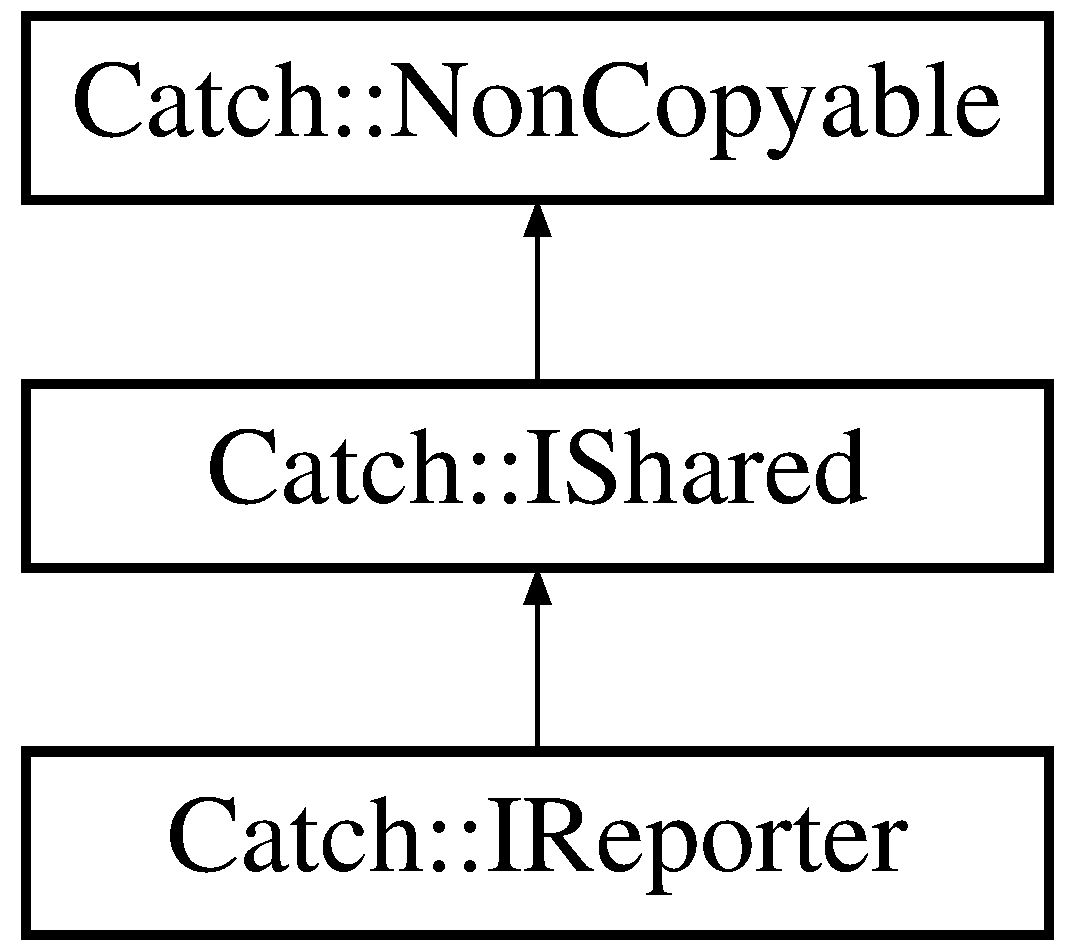
\includegraphics[height=3.000000cm]{structCatch_1_1IShared}
\end{center}
\end{figure}
\subsubsection*{Public Member Functions}
\begin{DoxyCompactItemize}
\item 
virtual \hyperlink{structCatch_1_1IShared_a5e842e7540ae7ae0c62a2758123503f6}{$\sim$\-I\-Shared} ()
\item 
virtual void \hyperlink{structCatch_1_1IShared_aebc526a44fbca6f94d5946c05e8897bd}{add\-Ref} ()=0
\item 
virtual void \hyperlink{structCatch_1_1IShared_a47f50205a327631f58793267b4da5e8a}{release} ()=0
\end{DoxyCompactItemize}
\subsubsection*{Additional Inherited Members}


\subsubsection{Constructor \& Destructor Documentation}
\hypertarget{structCatch_1_1IShared_a5e842e7540ae7ae0c62a2758123503f6}{\index{Catch\-::\-I\-Shared@{Catch\-::\-I\-Shared}!$\sim$\-I\-Shared@{$\sim$\-I\-Shared}}
\index{$\sim$\-I\-Shared@{$\sim$\-I\-Shared}!Catch::IShared@{Catch\-::\-I\-Shared}}
\paragraph[{$\sim$\-I\-Shared}]{\setlength{\rightskip}{0pt plus 5cm}virtual Catch\-::\-I\-Shared\-::$\sim$\-I\-Shared (
\begin{DoxyParamCaption}
{}
\end{DoxyParamCaption}
)\hspace{0.3cm}{\ttfamily [inline]}, {\ttfamily [virtual]}}}\label{structCatch_1_1IShared_a5e842e7540ae7ae0c62a2758123503f6}


\subsubsection{Member Function Documentation}
\hypertarget{structCatch_1_1IShared_aebc526a44fbca6f94d5946c05e8897bd}{\index{Catch\-::\-I\-Shared@{Catch\-::\-I\-Shared}!add\-Ref@{add\-Ref}}
\index{add\-Ref@{add\-Ref}!Catch::IShared@{Catch\-::\-I\-Shared}}
\paragraph[{add\-Ref}]{\setlength{\rightskip}{0pt plus 5cm}virtual void Catch\-::\-I\-Shared\-::add\-Ref (
\begin{DoxyParamCaption}
{}
\end{DoxyParamCaption}
)\hspace{0.3cm}{\ttfamily [pure virtual]}}}\label{structCatch_1_1IShared_aebc526a44fbca6f94d5946c05e8897bd}
\hypertarget{structCatch_1_1IShared_a47f50205a327631f58793267b4da5e8a}{\index{Catch\-::\-I\-Shared@{Catch\-::\-I\-Shared}!release@{release}}
\index{release@{release}!Catch::IShared@{Catch\-::\-I\-Shared}}
\paragraph[{release}]{\setlength{\rightskip}{0pt plus 5cm}virtual void Catch\-::\-I\-Shared\-::release (
\begin{DoxyParamCaption}
{}
\end{DoxyParamCaption}
)\hspace{0.3cm}{\ttfamily [pure virtual]}}}\label{structCatch_1_1IShared_a47f50205a327631f58793267b4da5e8a}


The documentation for this struct was generated from the following file\-:\begin{DoxyCompactItemize}
\item 
include/\hyperlink{catch_8hpp}{catch.\-hpp}\end{DoxyCompactItemize}

\hypertarget{structCatch_1_1ITestCase}{\subsection{Catch\-:\-:I\-Test\-Case Struct Reference}
\label{structCatch_1_1ITestCase}\index{Catch\-::\-I\-Test\-Case@{Catch\-::\-I\-Test\-Case}}
}


{\ttfamily \#include $<$catch.\-hpp$>$}

Inheritance diagram for Catch\-:\-:I\-Test\-Case\-:\begin{figure}[H]
\begin{center}
\leavevmode
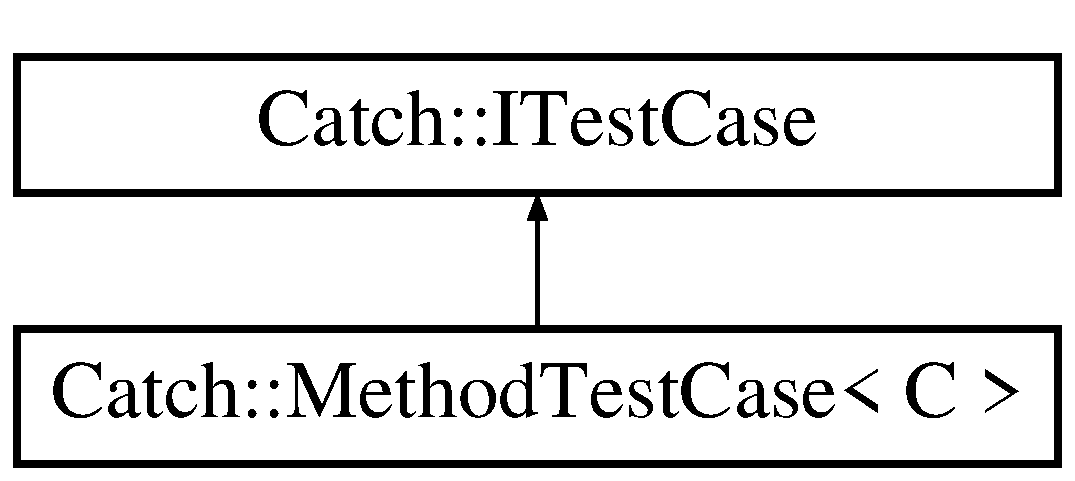
\includegraphics[height=2.000000cm]{structCatch_1_1ITestCase}
\end{center}
\end{figure}
\subsubsection*{Public Member Functions}
\begin{DoxyCompactItemize}
\item 
virtual \hyperlink{structCatch_1_1ITestCase_add7b9bec455ac1b007c17df82144310e}{$\sim$\-I\-Test\-Case} ()
\item 
virtual void \hyperlink{structCatch_1_1ITestCase_a678825e62e7c17297621cfeb65588c34}{invoke} () const =0
\item 
virtual \hyperlink{structCatch_1_1ITestCase}{I\-Test\-Case} $\ast$ \hyperlink{structCatch_1_1ITestCase_af5307c170b81e94c14dc3d64ce598340}{clone} () const =0
\item 
virtual bool \hyperlink{structCatch_1_1ITestCase_a21ba9bd73bbf9c8e0384ed94d0f4cbb9}{operator==} (const \hyperlink{structCatch_1_1ITestCase}{I\-Test\-Case} \&other) const =0
\item 
virtual bool \hyperlink{structCatch_1_1ITestCase_aae3e96da1a4494890326db813c010ddb}{operator$<$} (const \hyperlink{structCatch_1_1ITestCase}{I\-Test\-Case} \&other) const =0
\end{DoxyCompactItemize}


\subsubsection{Constructor \& Destructor Documentation}
\hypertarget{structCatch_1_1ITestCase_add7b9bec455ac1b007c17df82144310e}{\index{Catch\-::\-I\-Test\-Case@{Catch\-::\-I\-Test\-Case}!$\sim$\-I\-Test\-Case@{$\sim$\-I\-Test\-Case}}
\index{$\sim$\-I\-Test\-Case@{$\sim$\-I\-Test\-Case}!Catch::ITestCase@{Catch\-::\-I\-Test\-Case}}
\paragraph[{$\sim$\-I\-Test\-Case}]{\setlength{\rightskip}{0pt plus 5cm}virtual Catch\-::\-I\-Test\-Case\-::$\sim$\-I\-Test\-Case (
\begin{DoxyParamCaption}
{}
\end{DoxyParamCaption}
)\hspace{0.3cm}{\ttfamily [inline]}, {\ttfamily [virtual]}}}\label{structCatch_1_1ITestCase_add7b9bec455ac1b007c17df82144310e}


\subsubsection{Member Function Documentation}
\hypertarget{structCatch_1_1ITestCase_af5307c170b81e94c14dc3d64ce598340}{\index{Catch\-::\-I\-Test\-Case@{Catch\-::\-I\-Test\-Case}!clone@{clone}}
\index{clone@{clone}!Catch::ITestCase@{Catch\-::\-I\-Test\-Case}}
\paragraph[{clone}]{\setlength{\rightskip}{0pt plus 5cm}virtual {\bf I\-Test\-Case}$\ast$ Catch\-::\-I\-Test\-Case\-::clone (
\begin{DoxyParamCaption}
{}
\end{DoxyParamCaption}
) const\hspace{0.3cm}{\ttfamily [pure virtual]}}}\label{structCatch_1_1ITestCase_af5307c170b81e94c14dc3d64ce598340}


Implemented in \hyperlink{classCatch_1_1MethodTestCase_a11448e37336915c7f93d470b4c517961}{Catch\-::\-Method\-Test\-Case$<$ C $>$}.

\hypertarget{structCatch_1_1ITestCase_a678825e62e7c17297621cfeb65588c34}{\index{Catch\-::\-I\-Test\-Case@{Catch\-::\-I\-Test\-Case}!invoke@{invoke}}
\index{invoke@{invoke}!Catch::ITestCase@{Catch\-::\-I\-Test\-Case}}
\paragraph[{invoke}]{\setlength{\rightskip}{0pt plus 5cm}virtual void Catch\-::\-I\-Test\-Case\-::invoke (
\begin{DoxyParamCaption}
{}
\end{DoxyParamCaption}
) const\hspace{0.3cm}{\ttfamily [pure virtual]}}}\label{structCatch_1_1ITestCase_a678825e62e7c17297621cfeb65588c34}


Implemented in \hyperlink{classCatch_1_1MethodTestCase_a39cc4b760dd71adc3f7550bc1e7eb697}{Catch\-::\-Method\-Test\-Case$<$ C $>$}.

\hypertarget{structCatch_1_1ITestCase_aae3e96da1a4494890326db813c010ddb}{\index{Catch\-::\-I\-Test\-Case@{Catch\-::\-I\-Test\-Case}!operator$<$@{operator$<$}}
\index{operator$<$@{operator$<$}!Catch::ITestCase@{Catch\-::\-I\-Test\-Case}}
\paragraph[{operator$<$}]{\setlength{\rightskip}{0pt plus 5cm}virtual bool Catch\-::\-I\-Test\-Case\-::operator$<$ (
\begin{DoxyParamCaption}
\item[{const {\bf I\-Test\-Case} \&}]{other}
\end{DoxyParamCaption}
) const\hspace{0.3cm}{\ttfamily [pure virtual]}}}\label{structCatch_1_1ITestCase_aae3e96da1a4494890326db813c010ddb}


Implemented in \hyperlink{classCatch_1_1MethodTestCase_ac411bdeb5057d7e32ef64e1287debbef}{Catch\-::\-Method\-Test\-Case$<$ C $>$}.

\hypertarget{structCatch_1_1ITestCase_a21ba9bd73bbf9c8e0384ed94d0f4cbb9}{\index{Catch\-::\-I\-Test\-Case@{Catch\-::\-I\-Test\-Case}!operator==@{operator==}}
\index{operator==@{operator==}!Catch::ITestCase@{Catch\-::\-I\-Test\-Case}}
\paragraph[{operator==}]{\setlength{\rightskip}{0pt plus 5cm}virtual bool Catch\-::\-I\-Test\-Case\-::operator== (
\begin{DoxyParamCaption}
\item[{const {\bf I\-Test\-Case} \&}]{other}
\end{DoxyParamCaption}
) const\hspace{0.3cm}{\ttfamily [pure virtual]}}}\label{structCatch_1_1ITestCase_a21ba9bd73bbf9c8e0384ed94d0f4cbb9}


Implemented in \hyperlink{classCatch_1_1MethodTestCase_a78295dacec5d279e6ea312c6af9aebb0}{Catch\-::\-Method\-Test\-Case$<$ C $>$}.



The documentation for this struct was generated from the following file\-:\begin{DoxyCompactItemize}
\item 
include/\hyperlink{catch_8hpp}{catch.\-hpp}\end{DoxyCompactItemize}

\hypertarget{structCatch_1_1ITestCaseRegistry}{\subsection{Catch\-:\-:I\-Test\-Case\-Registry Struct Reference}
\label{structCatch_1_1ITestCaseRegistry}\index{Catch\-::\-I\-Test\-Case\-Registry@{Catch\-::\-I\-Test\-Case\-Registry}}
}


{\ttfamily \#include $<$catch.\-hpp$>$}

\subsubsection*{Public Member Functions}
\begin{DoxyCompactItemize}
\item 
virtual \hyperlink{structCatch_1_1ITestCaseRegistry_ae14798f05ac8e2b18cff532849a4da81}{$\sim$\-I\-Test\-Case\-Registry} ()
\item 
virtual void \hyperlink{structCatch_1_1ITestCaseRegistry_a0b4e7f4f450bd3f2ea8ab48f7927a233}{register\-Test} (const \hyperlink{classCatch_1_1TestCaseInfo}{Test\-Case\-Info} \&test\-Info)=0
\item 
virtual const std\-::vector\\*
$<$ \hyperlink{classCatch_1_1TestCaseInfo}{Test\-Case\-Info} $>$ \& \hyperlink{structCatch_1_1ITestCaseRegistry_ae61a69ef1262764ba69c6aed48890a6b}{get\-All\-Tests} () const =0
\item 
virtual std\-::vector$<$ \hyperlink{classCatch_1_1TestCaseInfo}{Test\-Case\-Info} $>$ \hyperlink{structCatch_1_1ITestCaseRegistry_aff5d343c12bf490aca3a4b6ea097c8c0}{get\-Matching\-Test\-Cases} (const std\-::string \&raw\-Test\-Spec)=0
\end{DoxyCompactItemize}


\subsubsection{Constructor \& Destructor Documentation}
\hypertarget{structCatch_1_1ITestCaseRegistry_ae14798f05ac8e2b18cff532849a4da81}{\index{Catch\-::\-I\-Test\-Case\-Registry@{Catch\-::\-I\-Test\-Case\-Registry}!$\sim$\-I\-Test\-Case\-Registry@{$\sim$\-I\-Test\-Case\-Registry}}
\index{$\sim$\-I\-Test\-Case\-Registry@{$\sim$\-I\-Test\-Case\-Registry}!Catch::ITestCaseRegistry@{Catch\-::\-I\-Test\-Case\-Registry}}
\paragraph[{$\sim$\-I\-Test\-Case\-Registry}]{\setlength{\rightskip}{0pt plus 5cm}virtual Catch\-::\-I\-Test\-Case\-Registry\-::$\sim$\-I\-Test\-Case\-Registry (
\begin{DoxyParamCaption}
{}
\end{DoxyParamCaption}
)\hspace{0.3cm}{\ttfamily [inline]}, {\ttfamily [virtual]}}}\label{structCatch_1_1ITestCaseRegistry_ae14798f05ac8e2b18cff532849a4da81}


\subsubsection{Member Function Documentation}
\hypertarget{structCatch_1_1ITestCaseRegistry_ae61a69ef1262764ba69c6aed48890a6b}{\index{Catch\-::\-I\-Test\-Case\-Registry@{Catch\-::\-I\-Test\-Case\-Registry}!get\-All\-Tests@{get\-All\-Tests}}
\index{get\-All\-Tests@{get\-All\-Tests}!Catch::ITestCaseRegistry@{Catch\-::\-I\-Test\-Case\-Registry}}
\paragraph[{get\-All\-Tests}]{\setlength{\rightskip}{0pt plus 5cm}virtual const std\-::vector$<${\bf Test\-Case\-Info}$>$\& Catch\-::\-I\-Test\-Case\-Registry\-::get\-All\-Tests (
\begin{DoxyParamCaption}
{}
\end{DoxyParamCaption}
) const\hspace{0.3cm}{\ttfamily [pure virtual]}}}\label{structCatch_1_1ITestCaseRegistry_ae61a69ef1262764ba69c6aed48890a6b}
\hypertarget{structCatch_1_1ITestCaseRegistry_aff5d343c12bf490aca3a4b6ea097c8c0}{\index{Catch\-::\-I\-Test\-Case\-Registry@{Catch\-::\-I\-Test\-Case\-Registry}!get\-Matching\-Test\-Cases@{get\-Matching\-Test\-Cases}}
\index{get\-Matching\-Test\-Cases@{get\-Matching\-Test\-Cases}!Catch::ITestCaseRegistry@{Catch\-::\-I\-Test\-Case\-Registry}}
\paragraph[{get\-Matching\-Test\-Cases}]{\setlength{\rightskip}{0pt plus 5cm}virtual std\-::vector$<${\bf Test\-Case\-Info}$>$ Catch\-::\-I\-Test\-Case\-Registry\-::get\-Matching\-Test\-Cases (
\begin{DoxyParamCaption}
\item[{const std\-::string \&}]{raw\-Test\-Spec}
\end{DoxyParamCaption}
)\hspace{0.3cm}{\ttfamily [pure virtual]}}}\label{structCatch_1_1ITestCaseRegistry_aff5d343c12bf490aca3a4b6ea097c8c0}
\hypertarget{structCatch_1_1ITestCaseRegistry_a0b4e7f4f450bd3f2ea8ab48f7927a233}{\index{Catch\-::\-I\-Test\-Case\-Registry@{Catch\-::\-I\-Test\-Case\-Registry}!register\-Test@{register\-Test}}
\index{register\-Test@{register\-Test}!Catch::ITestCaseRegistry@{Catch\-::\-I\-Test\-Case\-Registry}}
\paragraph[{register\-Test}]{\setlength{\rightskip}{0pt plus 5cm}virtual void Catch\-::\-I\-Test\-Case\-Registry\-::register\-Test (
\begin{DoxyParamCaption}
\item[{const {\bf Test\-Case\-Info} \&}]{test\-Info}
\end{DoxyParamCaption}
)\hspace{0.3cm}{\ttfamily [pure virtual]}}}\label{structCatch_1_1ITestCaseRegistry_a0b4e7f4f450bd3f2ea8ab48f7927a233}


The documentation for this struct was generated from the following file\-:\begin{DoxyCompactItemize}
\item 
include/\hyperlink{catch_8hpp}{catch.\-hpp}\end{DoxyCompactItemize}

\hypertarget{structKLTFeatureTrackingParameters}{\subsection{K\-L\-T\-Feature\-Tracking\-Parameters Struct Reference}
\label{structKLTFeatureTrackingParameters}\index{K\-L\-T\-Feature\-Tracking\-Parameters@{K\-L\-T\-Feature\-Tracking\-Parameters}}
}


{\ttfamily \#include $<$Parameters.\-hpp$>$}

\subsubsection*{Public Member Functions}
\begin{DoxyCompactItemize}
\item 
\hyperlink{structKLTFeatureTrackingParameters_afb176376d930d5aad8064535835830ec}{K\-L\-T\-Feature\-Tracking\-Parameters} (const int argc, char $\ast$argv\mbox{[}$\,$\mbox{]})
\item 
std\-::string \hyperlink{structKLTFeatureTrackingParameters_a2debf68a0b959e1e02316f905c7e0a79}{get\-Parameter\-Description} (boost\-::program\-\_\-options\-::options\-\_\-description \&options, const boost\-::program\-\_\-options\-::variables\-\_\-map \&vm, const std\-::string \&separator=\char`\"{} \char`\"{}) const 
\end{DoxyCompactItemize}
\subsubsection*{Public Attributes}
\begin{DoxyCompactItemize}
\item 
bool \hyperlink{structKLTFeatureTrackingParameters_a2f9e1e592d223893da0a10a918041478}{track\-Features}
\item 
bool \hyperlink{structKLTFeatureTrackingParameters_ae6be9a8b6eef4c1e0a2628f1c245eb91}{group\-Features}
\item 
bool \hyperlink{structKLTFeatureTrackingParameters_ad8e4778a92dc382ad832c32034c166cb}{loading\-Time}
\item 
std\-::string \hyperlink{structKLTFeatureTrackingParameters_a87b8566bf24da095bacc06392f05076d}{video\-Filename}
\item 
std\-::string \hyperlink{structKLTFeatureTrackingParameters_ab3e88594375e51a2a1df46e3a43fe059}{database\-Filename}
\item 
std\-::string \hyperlink{structKLTFeatureTrackingParameters_acf597dff26e9c6ca5baa54ccf1aca168}{homography\-Filename}
\item 
std\-::string \hyperlink{structKLTFeatureTrackingParameters_a42414b788b278cc5c82ae56138629244}{intrinsic\-Camera\-Filename}
\item 
std\-::vector$<$ float $>$ \hyperlink{structKLTFeatureTrackingParameters_a669fd53774f24cb51afdd226c4cbe4fc}{distortion\-Coefficients}
\item 
float \hyperlink{structKLTFeatureTrackingParameters_ac22e64f140b123564df5f1d07dcd59bb}{undistorted\-Image\-Multiplication}
\item 
int \hyperlink{structKLTFeatureTrackingParameters_a94e4b6d4684854aec07e22e76e08bbf9}{interpolation\-Method}
\item 
std\-::string \hyperlink{structKLTFeatureTrackingParameters_aa32f95fc8ca3200bde536122aaad01d3}{mask\-Filename}
\item 
bool \hyperlink{structKLTFeatureTrackingParameters_aab76e7ff65dedfb16d14dc4c17d50611}{undistort}
\item 
bool \hyperlink{structKLTFeatureTrackingParameters_a9c8bb8bc271d18ef336bb4cc87dfa62e}{load\-Features}
\item 
bool \hyperlink{structKLTFeatureTrackingParameters_a2751a5a7daba84d0ec5595ead46cfd2b}{display}
\item 
float \hyperlink{structKLTFeatureTrackingParameters_aaa2efb4d7c7c2a9899501b8978278db5}{video\-F\-P\-S}
\item 
unsigned int \hyperlink{structKLTFeatureTrackingParameters_a5cfd406341b9cfc06682c68450034840}{frame1}
\item 
int \hyperlink{structKLTFeatureTrackingParameters_a0c3b89582f2105d0dc3da8f599518031}{n\-Frames}
\item 
int \hyperlink{structKLTFeatureTrackingParameters_a89edeff35aebc548921ea9b6a3501c53}{max\-N\-Features}
\begin{DoxyCompactList}\small\item\em \char`\"{}\-Maximum number of corners to return\char`\"{} (Open\-C\-V good\-Features\-To\-Track) (should be large enough not to limit the potential number of features) \end{DoxyCompactList}\item 
float \hyperlink{structKLTFeatureTrackingParameters_a062d49d0d11189735724e049d9f72765}{feature\-Quality}
\begin{DoxyCompactList}\small\item\em \char`\"{}\-Parameter characterizing the minimal accepted quality of image corners\char`\"{} (Open\-C\-V good\-Features\-To\-Track ) \end{DoxyCompactList}\item 
float \hyperlink{structKLTFeatureTrackingParameters_af9ba36e53a3954620a535fdee4f04686}{min\-Feature\-Distance\-K\-L\-T}
\begin{DoxyCompactList}\small\item\em \char`\"{}\-Minimum possible Euclidean distance between the returned corners\char`\"{} (Open\-C\-V good\-Features\-To\-Track) \end{DoxyCompactList}\item 
int \hyperlink{structKLTFeatureTrackingParameters_af223c42de0f06da1a786451c2d379130}{block\-Size}
\begin{DoxyCompactList}\small\item\em \char`\"{}\-Size of an average block for computing a derivative covariation matrix over each pixel neighborhood\char`\"{} (Open\-C\-V good\-Features\-To\-Track) \end{DoxyCompactList}\item 
bool \hyperlink{structKLTFeatureTrackingParameters_a5157702aea82ce0d2e8a497dd9182c70}{use\-Harris\-Detector}
\begin{DoxyCompactList}\small\item\em \char`\"{}\-Parameter indicating whether to use a Harris detector\char`\"{} (Open\-C\-V good\-Features\-To\-Track) \end{DoxyCompactList}\item 
float \hyperlink{structKLTFeatureTrackingParameters_a6a959cf31cc7e44c36f6cd50b29ef11b}{k}
\begin{DoxyCompactList}\small\item\em \char`\"{}\-Free parameter of the Harris detector\char`\"{} (Open\-C\-V good\-Features\-To\-Track) \end{DoxyCompactList}\item 
int \hyperlink{structKLTFeatureTrackingParameters_a95b45dfb47f9f26633b252d3f4a68df3}{window\-Size}
\begin{DoxyCompactList}\small\item\em \char`\"{}size of the search window at each pyramid level\char`\"{} (Open\-C\-V calc\-Optical\-Flow\-Pyr\-L\-K) \end{DoxyCompactList}\item 
int \hyperlink{structKLTFeatureTrackingParameters_aeba87313d1ee04d20c8edbbc974a80ac}{pyramid\-Level}
\begin{DoxyCompactList}\small\item\em \char`\"{}0-\/based maximal pyramid level number\char`\"{} (Open\-C\-V calc\-Optical\-Flow\-Pyr\-L\-K) higher is higher quality \end{DoxyCompactList}\item 
unsigned int \hyperlink{structKLTFeatureTrackingParameters_a1b5dba549536ac01c2817a63c138b9a7}{n\-Displacements}
\begin{DoxyCompactList}\small\item\em Number of displacements (number of frames-\/1) over which minimum motion is computed. \end{DoxyCompactList}\item 
float \hyperlink{structKLTFeatureTrackingParameters_a77753bc52f8cf4dd6f9e7f0061f24fe9}{min\-Feature\-Displacement}
\begin{DoxyCompactList}\small\item\em Minimum displacement per frame (in world space) to keep features. \end{DoxyCompactList}\item 
float \hyperlink{structKLTFeatureTrackingParameters_a3d39ac0306730636b9f3ac94ea7448d1}{acceleration\-Bound}
\begin{DoxyCompactList}\small\item\em Maximum feature acceleration. \end{DoxyCompactList}\item 
float \hyperlink{structKLTFeatureTrackingParameters_a692406d82ec8adad42321e13a7c6e9af}{deviation\-Bound}
\begin{DoxyCompactList}\small\item\em Maximum feature deviation. \end{DoxyCompactList}\item 
int \hyperlink{structKLTFeatureTrackingParameters_ad5a4d722c17641c805483790fda819c9}{n\-Frames\-Smoothing}
\begin{DoxyCompactList}\small\item\em Number of frames to smooth positions (half window) \end{DoxyCompactList}\item 
int \hyperlink{structKLTFeatureTrackingParameters_a491f9f95b04854f413e2a262d32c0ae3}{max\-Number\-Tracking\-Iterations}
\begin{DoxyCompactList}\small\item\em Maximum number of iterations to stop optical flow (Open\-C\-V calc\-Optical\-Flow\-Pyr\-L\-K) \end{DoxyCompactList}\item 
float \hyperlink{structKLTFeatureTrackingParameters_a52dd1c8d9b949260f7715f5fa705217e}{min\-Tracking\-Error}
\begin{DoxyCompactList}\small\item\em Minimum error to reach to stop optical flow (Open\-C\-V calc\-Optical\-Flow\-Pyr\-L\-K) \end{DoxyCompactList}\item 
float \hyperlink{structKLTFeatureTrackingParameters_a9276bdc0bbba6a06cab152993a774be8}{min\-Feature\-Eig\-Threshold}
\begin{DoxyCompactList}\small\item\em Minimum eigen value of a 2x2 normal matrix of optical flow equations (Open\-C\-V calc\-Optical\-Flow\-Pyr\-L\-K) \end{DoxyCompactList}\item 
unsigned int \hyperlink{structKLTFeatureTrackingParameters_ae695d0f6bf3e578e744ae94f85b53009}{min\-Feature\-Time}
\begin{DoxyCompactList}\small\item\em Minimum length of a feature (number of frames) to consider a feature for grouping. \end{DoxyCompactList}\item 
float \hyperlink{structKLTFeatureTrackingParameters_a83a3fbc2ab0c369b8ccda3d1669ed988}{mm\-Connection\-Distance}
\begin{DoxyCompactList}\small\item\em Connection distance in feature grouping (in world space) \end{DoxyCompactList}\item 
float \hyperlink{structKLTFeatureTrackingParameters_a2cf9367a2414ead952228bed67339e7c}{mm\-Segmentation\-Distance}
\begin{DoxyCompactList}\small\item\em Segmentation distance in feature grouping (in world space) \end{DoxyCompactList}\item 
float \hyperlink{structKLTFeatureTrackingParameters_aa4870c94cfe88eb27b0b7bb75f6fed23}{max\-Distance}
\begin{DoxyCompactList}\small\item\em Maximum distance between features for grouping (in world space) (unused) \end{DoxyCompactList}\item 
float \hyperlink{structKLTFeatureTrackingParameters_a21ffaaa5b36521d31550438b6248b48d}{min\-Velocity\-Cosine}
\begin{DoxyCompactList}\small\item\em Minimum cosine of the angle between the velocity vectors for grouping (unused) \end{DoxyCompactList}\item 
float \hyperlink{structKLTFeatureTrackingParameters_a566bca052479db63d09155290e1e9106}{min\-N\-Features\-Per\-Group}
\begin{DoxyCompactList}\small\item\em Minimum average number of features per frame to create a vehicle hypothesis. \end{DoxyCompactList}\item 
float \hyperlink{structKLTFeatureTrackingParameters_ab363db8735a2d3f182e6d7c634b1cbf9}{max\-Predicted\-Speed}
\item 
float \hyperlink{structKLTFeatureTrackingParameters_adab4df4e7e0cbc6832ccf3380ddfa4f3}{prediction\-Time\-Horizon}
\item 
float \hyperlink{structKLTFeatureTrackingParameters_a79642a411853fb5eb8b17a190c80be26}{collision\-Distance}
\item 
bool \hyperlink{structKLTFeatureTrackingParameters_a6882da3735cb71f000283f2be17de08f}{crossing\-Zones}
\item 
std\-::string \hyperlink{structKLTFeatureTrackingParameters_a859980b7c56fab3a0a078a0b00290633}{prediction\-Method}
\item 
int \hyperlink{structKLTFeatureTrackingParameters_aeccd47f27aba6c9eafde449ee906431e}{n\-Predicted\-Trajectories}
\item 
float \hyperlink{structKLTFeatureTrackingParameters_a2f4e1ea73d5647a9b1a31c4aa2c7d829}{min\-Acceleration}
\item 
float \hyperlink{structKLTFeatureTrackingParameters_af41bb2da98e33adbe47c0f77989c5196}{max\-Acceleration}
\item 
float \hyperlink{structKLTFeatureTrackingParameters_ab3c794e5625524418d88cf00fc986c06}{max\-Steering}
\item 
bool \hyperlink{structKLTFeatureTrackingParameters_a66a200aa017c2c8c6928b5b06be858bd}{use\-Features\-For\-Prediction}
\item 
std\-::string \hyperlink{structKLTFeatureTrackingParameters_a7481415da28e5cb582d79690521f5087}{parameter\-Description}
\end{DoxyCompactItemize}


\subsubsection{Constructor \& Destructor Documentation}
\hypertarget{structKLTFeatureTrackingParameters_afb176376d930d5aad8064535835830ec}{\index{K\-L\-T\-Feature\-Tracking\-Parameters@{K\-L\-T\-Feature\-Tracking\-Parameters}!K\-L\-T\-Feature\-Tracking\-Parameters@{K\-L\-T\-Feature\-Tracking\-Parameters}}
\index{K\-L\-T\-Feature\-Tracking\-Parameters@{K\-L\-T\-Feature\-Tracking\-Parameters}!KLTFeatureTrackingParameters@{K\-L\-T\-Feature\-Tracking\-Parameters}}
\paragraph[{K\-L\-T\-Feature\-Tracking\-Parameters}]{\setlength{\rightskip}{0pt plus 5cm}K\-L\-T\-Feature\-Tracking\-Parameters\-::\-K\-L\-T\-Feature\-Tracking\-Parameters (
\begin{DoxyParamCaption}
\item[{const int}]{argc, }
\item[{char $\ast$}]{argv\mbox{[}$\,$\mbox{]}}
\end{DoxyParamCaption}
)}}\label{structKLTFeatureTrackingParameters_afb176376d930d5aad8064535835830ec}


References classify-\/objects\-::database\-Filename, display-\/trajectories\-::distortion\-Coefficients, group\-Features(), safety-\/analysis\-::prediction\-Method, track\-Features(), display-\/trajectories\-::undistort, display-\/trajectories\-::undistorted\-Image\-Multiplication, and classify-\/objects\-::video\-Filename.



\subsubsection{Member Function Documentation}
\hypertarget{structKLTFeatureTrackingParameters_a2debf68a0b959e1e02316f905c7e0a79}{\index{K\-L\-T\-Feature\-Tracking\-Parameters@{K\-L\-T\-Feature\-Tracking\-Parameters}!get\-Parameter\-Description@{get\-Parameter\-Description}}
\index{get\-Parameter\-Description@{get\-Parameter\-Description}!KLTFeatureTrackingParameters@{K\-L\-T\-Feature\-Tracking\-Parameters}}
\paragraph[{get\-Parameter\-Description}]{\setlength{\rightskip}{0pt plus 5cm}string K\-L\-T\-Feature\-Tracking\-Parameters\-::get\-Parameter\-Description (
\begin{DoxyParamCaption}
\item[{boost\-::program\-\_\-options\-::options\-\_\-description \&}]{options, }
\item[{const boost\-::program\-\_\-options\-::variables\-\_\-map \&}]{vm, }
\item[{const std\-::string \&}]{separator = {\ttfamily \char`\"{}~\char`\"{}}}
\end{DoxyParamCaption}
) const}}\label{structKLTFeatureTrackingParameters_a2debf68a0b959e1e02316f905c7e0a79}


\subsubsection{Member Data Documentation}
\hypertarget{structKLTFeatureTrackingParameters_a3d39ac0306730636b9f3ac94ea7448d1}{\index{K\-L\-T\-Feature\-Tracking\-Parameters@{K\-L\-T\-Feature\-Tracking\-Parameters}!acceleration\-Bound@{acceleration\-Bound}}
\index{acceleration\-Bound@{acceleration\-Bound}!KLTFeatureTrackingParameters@{K\-L\-T\-Feature\-Tracking\-Parameters}}
\paragraph[{acceleration\-Bound}]{\setlength{\rightskip}{0pt plus 5cm}float K\-L\-T\-Feature\-Tracking\-Parameters\-::acceleration\-Bound}}\label{structKLTFeatureTrackingParameters_a3d39ac0306730636b9f3ac94ea7448d1}


Maximum feature acceleration. 

\hypertarget{structKLTFeatureTrackingParameters_af223c42de0f06da1a786451c2d379130}{\index{K\-L\-T\-Feature\-Tracking\-Parameters@{K\-L\-T\-Feature\-Tracking\-Parameters}!block\-Size@{block\-Size}}
\index{block\-Size@{block\-Size}!KLTFeatureTrackingParameters@{K\-L\-T\-Feature\-Tracking\-Parameters}}
\paragraph[{block\-Size}]{\setlength{\rightskip}{0pt plus 5cm}int K\-L\-T\-Feature\-Tracking\-Parameters\-::block\-Size}}\label{structKLTFeatureTrackingParameters_af223c42de0f06da1a786451c2d379130}


\char`\"{}\-Size of an average block for computing a derivative covariation matrix over each pixel neighborhood\char`\"{} (Open\-C\-V good\-Features\-To\-Track) 

\hypertarget{structKLTFeatureTrackingParameters_a79642a411853fb5eb8b17a190c80be26}{\index{K\-L\-T\-Feature\-Tracking\-Parameters@{K\-L\-T\-Feature\-Tracking\-Parameters}!collision\-Distance@{collision\-Distance}}
\index{collision\-Distance@{collision\-Distance}!KLTFeatureTrackingParameters@{K\-L\-T\-Feature\-Tracking\-Parameters}}
\paragraph[{collision\-Distance}]{\setlength{\rightskip}{0pt plus 5cm}float K\-L\-T\-Feature\-Tracking\-Parameters\-::collision\-Distance}}\label{structKLTFeatureTrackingParameters_a79642a411853fb5eb8b17a190c80be26}
\hypertarget{structKLTFeatureTrackingParameters_a6882da3735cb71f000283f2be17de08f}{\index{K\-L\-T\-Feature\-Tracking\-Parameters@{K\-L\-T\-Feature\-Tracking\-Parameters}!crossing\-Zones@{crossing\-Zones}}
\index{crossing\-Zones@{crossing\-Zones}!KLTFeatureTrackingParameters@{K\-L\-T\-Feature\-Tracking\-Parameters}}
\paragraph[{crossing\-Zones}]{\setlength{\rightskip}{0pt plus 5cm}bool K\-L\-T\-Feature\-Tracking\-Parameters\-::crossing\-Zones}}\label{structKLTFeatureTrackingParameters_a6882da3735cb71f000283f2be17de08f}
\hypertarget{structKLTFeatureTrackingParameters_ab3e88594375e51a2a1df46e3a43fe059}{\index{K\-L\-T\-Feature\-Tracking\-Parameters@{K\-L\-T\-Feature\-Tracking\-Parameters}!database\-Filename@{database\-Filename}}
\index{database\-Filename@{database\-Filename}!KLTFeatureTrackingParameters@{K\-L\-T\-Feature\-Tracking\-Parameters}}
\paragraph[{database\-Filename}]{\setlength{\rightskip}{0pt plus 5cm}std\-::string K\-L\-T\-Feature\-Tracking\-Parameters\-::database\-Filename}}\label{structKLTFeatureTrackingParameters_ab3e88594375e51a2a1df46e3a43fe059}
\hypertarget{structKLTFeatureTrackingParameters_a692406d82ec8adad42321e13a7c6e9af}{\index{K\-L\-T\-Feature\-Tracking\-Parameters@{K\-L\-T\-Feature\-Tracking\-Parameters}!deviation\-Bound@{deviation\-Bound}}
\index{deviation\-Bound@{deviation\-Bound}!KLTFeatureTrackingParameters@{K\-L\-T\-Feature\-Tracking\-Parameters}}
\paragraph[{deviation\-Bound}]{\setlength{\rightskip}{0pt plus 5cm}float K\-L\-T\-Feature\-Tracking\-Parameters\-::deviation\-Bound}}\label{structKLTFeatureTrackingParameters_a692406d82ec8adad42321e13a7c6e9af}


Maximum feature deviation. 

\hypertarget{structKLTFeatureTrackingParameters_a2751a5a7daba84d0ec5595ead46cfd2b}{\index{K\-L\-T\-Feature\-Tracking\-Parameters@{K\-L\-T\-Feature\-Tracking\-Parameters}!display@{display}}
\index{display@{display}!KLTFeatureTrackingParameters@{K\-L\-T\-Feature\-Tracking\-Parameters}}
\paragraph[{display}]{\setlength{\rightskip}{0pt plus 5cm}bool K\-L\-T\-Feature\-Tracking\-Parameters\-::display}}\label{structKLTFeatureTrackingParameters_a2751a5a7daba84d0ec5595ead46cfd2b}
\hypertarget{structKLTFeatureTrackingParameters_a669fd53774f24cb51afdd226c4cbe4fc}{\index{K\-L\-T\-Feature\-Tracking\-Parameters@{K\-L\-T\-Feature\-Tracking\-Parameters}!distortion\-Coefficients@{distortion\-Coefficients}}
\index{distortion\-Coefficients@{distortion\-Coefficients}!KLTFeatureTrackingParameters@{K\-L\-T\-Feature\-Tracking\-Parameters}}
\paragraph[{distortion\-Coefficients}]{\setlength{\rightskip}{0pt plus 5cm}std\-::vector$<$float$>$ K\-L\-T\-Feature\-Tracking\-Parameters\-::distortion\-Coefficients}}\label{structKLTFeatureTrackingParameters_a669fd53774f24cb51afdd226c4cbe4fc}
\hypertarget{structKLTFeatureTrackingParameters_a062d49d0d11189735724e049d9f72765}{\index{K\-L\-T\-Feature\-Tracking\-Parameters@{K\-L\-T\-Feature\-Tracking\-Parameters}!feature\-Quality@{feature\-Quality}}
\index{feature\-Quality@{feature\-Quality}!KLTFeatureTrackingParameters@{K\-L\-T\-Feature\-Tracking\-Parameters}}
\paragraph[{feature\-Quality}]{\setlength{\rightskip}{0pt plus 5cm}float K\-L\-T\-Feature\-Tracking\-Parameters\-::feature\-Quality}}\label{structKLTFeatureTrackingParameters_a062d49d0d11189735724e049d9f72765}


\char`\"{}\-Parameter characterizing the minimal accepted quality of image corners\char`\"{} (Open\-C\-V good\-Features\-To\-Track ) 

\hypertarget{structKLTFeatureTrackingParameters_a5cfd406341b9cfc06682c68450034840}{\index{K\-L\-T\-Feature\-Tracking\-Parameters@{K\-L\-T\-Feature\-Tracking\-Parameters}!frame1@{frame1}}
\index{frame1@{frame1}!KLTFeatureTrackingParameters@{K\-L\-T\-Feature\-Tracking\-Parameters}}
\paragraph[{frame1}]{\setlength{\rightskip}{0pt plus 5cm}unsigned int K\-L\-T\-Feature\-Tracking\-Parameters\-::frame1}}\label{structKLTFeatureTrackingParameters_a5cfd406341b9cfc06682c68450034840}
\hypertarget{structKLTFeatureTrackingParameters_ae6be9a8b6eef4c1e0a2628f1c245eb91}{\index{K\-L\-T\-Feature\-Tracking\-Parameters@{K\-L\-T\-Feature\-Tracking\-Parameters}!group\-Features@{group\-Features}}
\index{group\-Features@{group\-Features}!KLTFeatureTrackingParameters@{K\-L\-T\-Feature\-Tracking\-Parameters}}
\paragraph[{group\-Features}]{\setlength{\rightskip}{0pt plus 5cm}bool K\-L\-T\-Feature\-Tracking\-Parameters\-::group\-Features}}\label{structKLTFeatureTrackingParameters_ae6be9a8b6eef4c1e0a2628f1c245eb91}
\hypertarget{structKLTFeatureTrackingParameters_acf597dff26e9c6ca5baa54ccf1aca168}{\index{K\-L\-T\-Feature\-Tracking\-Parameters@{K\-L\-T\-Feature\-Tracking\-Parameters}!homography\-Filename@{homography\-Filename}}
\index{homography\-Filename@{homography\-Filename}!KLTFeatureTrackingParameters@{K\-L\-T\-Feature\-Tracking\-Parameters}}
\paragraph[{homography\-Filename}]{\setlength{\rightskip}{0pt plus 5cm}std\-::string K\-L\-T\-Feature\-Tracking\-Parameters\-::homography\-Filename}}\label{structKLTFeatureTrackingParameters_acf597dff26e9c6ca5baa54ccf1aca168}
\hypertarget{structKLTFeatureTrackingParameters_a94e4b6d4684854aec07e22e76e08bbf9}{\index{K\-L\-T\-Feature\-Tracking\-Parameters@{K\-L\-T\-Feature\-Tracking\-Parameters}!interpolation\-Method@{interpolation\-Method}}
\index{interpolation\-Method@{interpolation\-Method}!KLTFeatureTrackingParameters@{K\-L\-T\-Feature\-Tracking\-Parameters}}
\paragraph[{interpolation\-Method}]{\setlength{\rightskip}{0pt plus 5cm}int K\-L\-T\-Feature\-Tracking\-Parameters\-::interpolation\-Method}}\label{structKLTFeatureTrackingParameters_a94e4b6d4684854aec07e22e76e08bbf9}
\hypertarget{structKLTFeatureTrackingParameters_a42414b788b278cc5c82ae56138629244}{\index{K\-L\-T\-Feature\-Tracking\-Parameters@{K\-L\-T\-Feature\-Tracking\-Parameters}!intrinsic\-Camera\-Filename@{intrinsic\-Camera\-Filename}}
\index{intrinsic\-Camera\-Filename@{intrinsic\-Camera\-Filename}!KLTFeatureTrackingParameters@{K\-L\-T\-Feature\-Tracking\-Parameters}}
\paragraph[{intrinsic\-Camera\-Filename}]{\setlength{\rightskip}{0pt plus 5cm}std\-::string K\-L\-T\-Feature\-Tracking\-Parameters\-::intrinsic\-Camera\-Filename}}\label{structKLTFeatureTrackingParameters_a42414b788b278cc5c82ae56138629244}
\hypertarget{structKLTFeatureTrackingParameters_a6a959cf31cc7e44c36f6cd50b29ef11b}{\index{K\-L\-T\-Feature\-Tracking\-Parameters@{K\-L\-T\-Feature\-Tracking\-Parameters}!k@{k}}
\index{k@{k}!KLTFeatureTrackingParameters@{K\-L\-T\-Feature\-Tracking\-Parameters}}
\paragraph[{k}]{\setlength{\rightskip}{0pt plus 5cm}float K\-L\-T\-Feature\-Tracking\-Parameters\-::k}}\label{structKLTFeatureTrackingParameters_a6a959cf31cc7e44c36f6cd50b29ef11b}


\char`\"{}\-Free parameter of the Harris detector\char`\"{} (Open\-C\-V good\-Features\-To\-Track) 

\hypertarget{structKLTFeatureTrackingParameters_a9c8bb8bc271d18ef336bb4cc87dfa62e}{\index{K\-L\-T\-Feature\-Tracking\-Parameters@{K\-L\-T\-Feature\-Tracking\-Parameters}!load\-Features@{load\-Features}}
\index{load\-Features@{load\-Features}!KLTFeatureTrackingParameters@{K\-L\-T\-Feature\-Tracking\-Parameters}}
\paragraph[{load\-Features}]{\setlength{\rightskip}{0pt plus 5cm}bool K\-L\-T\-Feature\-Tracking\-Parameters\-::load\-Features}}\label{structKLTFeatureTrackingParameters_a9c8bb8bc271d18ef336bb4cc87dfa62e}
\hypertarget{structKLTFeatureTrackingParameters_ad8e4778a92dc382ad832c32034c166cb}{\index{K\-L\-T\-Feature\-Tracking\-Parameters@{K\-L\-T\-Feature\-Tracking\-Parameters}!loading\-Time@{loading\-Time}}
\index{loading\-Time@{loading\-Time}!KLTFeatureTrackingParameters@{K\-L\-T\-Feature\-Tracking\-Parameters}}
\paragraph[{loading\-Time}]{\setlength{\rightskip}{0pt plus 5cm}bool K\-L\-T\-Feature\-Tracking\-Parameters\-::loading\-Time}}\label{structKLTFeatureTrackingParameters_ad8e4778a92dc382ad832c32034c166cb}
\hypertarget{structKLTFeatureTrackingParameters_aa32f95fc8ca3200bde536122aaad01d3}{\index{K\-L\-T\-Feature\-Tracking\-Parameters@{K\-L\-T\-Feature\-Tracking\-Parameters}!mask\-Filename@{mask\-Filename}}
\index{mask\-Filename@{mask\-Filename}!KLTFeatureTrackingParameters@{K\-L\-T\-Feature\-Tracking\-Parameters}}
\paragraph[{mask\-Filename}]{\setlength{\rightskip}{0pt plus 5cm}std\-::string K\-L\-T\-Feature\-Tracking\-Parameters\-::mask\-Filename}}\label{structKLTFeatureTrackingParameters_aa32f95fc8ca3200bde536122aaad01d3}
\hypertarget{structKLTFeatureTrackingParameters_af41bb2da98e33adbe47c0f77989c5196}{\index{K\-L\-T\-Feature\-Tracking\-Parameters@{K\-L\-T\-Feature\-Tracking\-Parameters}!max\-Acceleration@{max\-Acceleration}}
\index{max\-Acceleration@{max\-Acceleration}!KLTFeatureTrackingParameters@{K\-L\-T\-Feature\-Tracking\-Parameters}}
\paragraph[{max\-Acceleration}]{\setlength{\rightskip}{0pt plus 5cm}float K\-L\-T\-Feature\-Tracking\-Parameters\-::max\-Acceleration}}\label{structKLTFeatureTrackingParameters_af41bb2da98e33adbe47c0f77989c5196}
\hypertarget{structKLTFeatureTrackingParameters_aa4870c94cfe88eb27b0b7bb75f6fed23}{\index{K\-L\-T\-Feature\-Tracking\-Parameters@{K\-L\-T\-Feature\-Tracking\-Parameters}!max\-Distance@{max\-Distance}}
\index{max\-Distance@{max\-Distance}!KLTFeatureTrackingParameters@{K\-L\-T\-Feature\-Tracking\-Parameters}}
\paragraph[{max\-Distance}]{\setlength{\rightskip}{0pt plus 5cm}float K\-L\-T\-Feature\-Tracking\-Parameters\-::max\-Distance}}\label{structKLTFeatureTrackingParameters_aa4870c94cfe88eb27b0b7bb75f6fed23}


Maximum distance between features for grouping (in world space) (unused) 

\hypertarget{structKLTFeatureTrackingParameters_a89edeff35aebc548921ea9b6a3501c53}{\index{K\-L\-T\-Feature\-Tracking\-Parameters@{K\-L\-T\-Feature\-Tracking\-Parameters}!max\-N\-Features@{max\-N\-Features}}
\index{max\-N\-Features@{max\-N\-Features}!KLTFeatureTrackingParameters@{K\-L\-T\-Feature\-Tracking\-Parameters}}
\paragraph[{max\-N\-Features}]{\setlength{\rightskip}{0pt plus 5cm}int K\-L\-T\-Feature\-Tracking\-Parameters\-::max\-N\-Features}}\label{structKLTFeatureTrackingParameters_a89edeff35aebc548921ea9b6a3501c53}


\char`\"{}\-Maximum number of corners to return\char`\"{} (Open\-C\-V good\-Features\-To\-Track) (should be large enough not to limit the potential number of features) 

\hypertarget{structKLTFeatureTrackingParameters_a491f9f95b04854f413e2a262d32c0ae3}{\index{K\-L\-T\-Feature\-Tracking\-Parameters@{K\-L\-T\-Feature\-Tracking\-Parameters}!max\-Number\-Tracking\-Iterations@{max\-Number\-Tracking\-Iterations}}
\index{max\-Number\-Tracking\-Iterations@{max\-Number\-Tracking\-Iterations}!KLTFeatureTrackingParameters@{K\-L\-T\-Feature\-Tracking\-Parameters}}
\paragraph[{max\-Number\-Tracking\-Iterations}]{\setlength{\rightskip}{0pt plus 5cm}int K\-L\-T\-Feature\-Tracking\-Parameters\-::max\-Number\-Tracking\-Iterations}}\label{structKLTFeatureTrackingParameters_a491f9f95b04854f413e2a262d32c0ae3}


Maximum number of iterations to stop optical flow (Open\-C\-V calc\-Optical\-Flow\-Pyr\-L\-K) 

\hypertarget{structKLTFeatureTrackingParameters_ab363db8735a2d3f182e6d7c634b1cbf9}{\index{K\-L\-T\-Feature\-Tracking\-Parameters@{K\-L\-T\-Feature\-Tracking\-Parameters}!max\-Predicted\-Speed@{max\-Predicted\-Speed}}
\index{max\-Predicted\-Speed@{max\-Predicted\-Speed}!KLTFeatureTrackingParameters@{K\-L\-T\-Feature\-Tracking\-Parameters}}
\paragraph[{max\-Predicted\-Speed}]{\setlength{\rightskip}{0pt plus 5cm}float K\-L\-T\-Feature\-Tracking\-Parameters\-::max\-Predicted\-Speed}}\label{structKLTFeatureTrackingParameters_ab363db8735a2d3f182e6d7c634b1cbf9}
\hypertarget{structKLTFeatureTrackingParameters_ab3c794e5625524418d88cf00fc986c06}{\index{K\-L\-T\-Feature\-Tracking\-Parameters@{K\-L\-T\-Feature\-Tracking\-Parameters}!max\-Steering@{max\-Steering}}
\index{max\-Steering@{max\-Steering}!KLTFeatureTrackingParameters@{K\-L\-T\-Feature\-Tracking\-Parameters}}
\paragraph[{max\-Steering}]{\setlength{\rightskip}{0pt plus 5cm}float K\-L\-T\-Feature\-Tracking\-Parameters\-::max\-Steering}}\label{structKLTFeatureTrackingParameters_ab3c794e5625524418d88cf00fc986c06}
\hypertarget{structKLTFeatureTrackingParameters_a2f4e1ea73d5647a9b1a31c4aa2c7d829}{\index{K\-L\-T\-Feature\-Tracking\-Parameters@{K\-L\-T\-Feature\-Tracking\-Parameters}!min\-Acceleration@{min\-Acceleration}}
\index{min\-Acceleration@{min\-Acceleration}!KLTFeatureTrackingParameters@{K\-L\-T\-Feature\-Tracking\-Parameters}}
\paragraph[{min\-Acceleration}]{\setlength{\rightskip}{0pt plus 5cm}float K\-L\-T\-Feature\-Tracking\-Parameters\-::min\-Acceleration}}\label{structKLTFeatureTrackingParameters_a2f4e1ea73d5647a9b1a31c4aa2c7d829}
\hypertarget{structKLTFeatureTrackingParameters_a77753bc52f8cf4dd6f9e7f0061f24fe9}{\index{K\-L\-T\-Feature\-Tracking\-Parameters@{K\-L\-T\-Feature\-Tracking\-Parameters}!min\-Feature\-Displacement@{min\-Feature\-Displacement}}
\index{min\-Feature\-Displacement@{min\-Feature\-Displacement}!KLTFeatureTrackingParameters@{K\-L\-T\-Feature\-Tracking\-Parameters}}
\paragraph[{min\-Feature\-Displacement}]{\setlength{\rightskip}{0pt plus 5cm}float K\-L\-T\-Feature\-Tracking\-Parameters\-::min\-Feature\-Displacement}}\label{structKLTFeatureTrackingParameters_a77753bc52f8cf4dd6f9e7f0061f24fe9}


Minimum displacement per frame (in world space) to keep features. 

\hypertarget{structKLTFeatureTrackingParameters_af9ba36e53a3954620a535fdee4f04686}{\index{K\-L\-T\-Feature\-Tracking\-Parameters@{K\-L\-T\-Feature\-Tracking\-Parameters}!min\-Feature\-Distance\-K\-L\-T@{min\-Feature\-Distance\-K\-L\-T}}
\index{min\-Feature\-Distance\-K\-L\-T@{min\-Feature\-Distance\-K\-L\-T}!KLTFeatureTrackingParameters@{K\-L\-T\-Feature\-Tracking\-Parameters}}
\paragraph[{min\-Feature\-Distance\-K\-L\-T}]{\setlength{\rightskip}{0pt plus 5cm}float K\-L\-T\-Feature\-Tracking\-Parameters\-::min\-Feature\-Distance\-K\-L\-T}}\label{structKLTFeatureTrackingParameters_af9ba36e53a3954620a535fdee4f04686}


\char`\"{}\-Minimum possible Euclidean distance between the returned corners\char`\"{} (Open\-C\-V good\-Features\-To\-Track) 

\hypertarget{structKLTFeatureTrackingParameters_a9276bdc0bbba6a06cab152993a774be8}{\index{K\-L\-T\-Feature\-Tracking\-Parameters@{K\-L\-T\-Feature\-Tracking\-Parameters}!min\-Feature\-Eig\-Threshold@{min\-Feature\-Eig\-Threshold}}
\index{min\-Feature\-Eig\-Threshold@{min\-Feature\-Eig\-Threshold}!KLTFeatureTrackingParameters@{K\-L\-T\-Feature\-Tracking\-Parameters}}
\paragraph[{min\-Feature\-Eig\-Threshold}]{\setlength{\rightskip}{0pt plus 5cm}float K\-L\-T\-Feature\-Tracking\-Parameters\-::min\-Feature\-Eig\-Threshold}}\label{structKLTFeatureTrackingParameters_a9276bdc0bbba6a06cab152993a774be8}


Minimum eigen value of a 2x2 normal matrix of optical flow equations (Open\-C\-V calc\-Optical\-Flow\-Pyr\-L\-K) 

\hypertarget{structKLTFeatureTrackingParameters_ae695d0f6bf3e578e744ae94f85b53009}{\index{K\-L\-T\-Feature\-Tracking\-Parameters@{K\-L\-T\-Feature\-Tracking\-Parameters}!min\-Feature\-Time@{min\-Feature\-Time}}
\index{min\-Feature\-Time@{min\-Feature\-Time}!KLTFeatureTrackingParameters@{K\-L\-T\-Feature\-Tracking\-Parameters}}
\paragraph[{min\-Feature\-Time}]{\setlength{\rightskip}{0pt plus 5cm}unsigned int K\-L\-T\-Feature\-Tracking\-Parameters\-::min\-Feature\-Time}}\label{structKLTFeatureTrackingParameters_ae695d0f6bf3e578e744ae94f85b53009}


Minimum length of a feature (number of frames) to consider a feature for grouping. 

\hypertarget{structKLTFeatureTrackingParameters_a566bca052479db63d09155290e1e9106}{\index{K\-L\-T\-Feature\-Tracking\-Parameters@{K\-L\-T\-Feature\-Tracking\-Parameters}!min\-N\-Features\-Per\-Group@{min\-N\-Features\-Per\-Group}}
\index{min\-N\-Features\-Per\-Group@{min\-N\-Features\-Per\-Group}!KLTFeatureTrackingParameters@{K\-L\-T\-Feature\-Tracking\-Parameters}}
\paragraph[{min\-N\-Features\-Per\-Group}]{\setlength{\rightskip}{0pt plus 5cm}float K\-L\-T\-Feature\-Tracking\-Parameters\-::min\-N\-Features\-Per\-Group}}\label{structKLTFeatureTrackingParameters_a566bca052479db63d09155290e1e9106}


Minimum average number of features per frame to create a vehicle hypothesis. 

\hypertarget{structKLTFeatureTrackingParameters_a52dd1c8d9b949260f7715f5fa705217e}{\index{K\-L\-T\-Feature\-Tracking\-Parameters@{K\-L\-T\-Feature\-Tracking\-Parameters}!min\-Tracking\-Error@{min\-Tracking\-Error}}
\index{min\-Tracking\-Error@{min\-Tracking\-Error}!KLTFeatureTrackingParameters@{K\-L\-T\-Feature\-Tracking\-Parameters}}
\paragraph[{min\-Tracking\-Error}]{\setlength{\rightskip}{0pt plus 5cm}float K\-L\-T\-Feature\-Tracking\-Parameters\-::min\-Tracking\-Error}}\label{structKLTFeatureTrackingParameters_a52dd1c8d9b949260f7715f5fa705217e}


Minimum error to reach to stop optical flow (Open\-C\-V calc\-Optical\-Flow\-Pyr\-L\-K) 

\hypertarget{structKLTFeatureTrackingParameters_a21ffaaa5b36521d31550438b6248b48d}{\index{K\-L\-T\-Feature\-Tracking\-Parameters@{K\-L\-T\-Feature\-Tracking\-Parameters}!min\-Velocity\-Cosine@{min\-Velocity\-Cosine}}
\index{min\-Velocity\-Cosine@{min\-Velocity\-Cosine}!KLTFeatureTrackingParameters@{K\-L\-T\-Feature\-Tracking\-Parameters}}
\paragraph[{min\-Velocity\-Cosine}]{\setlength{\rightskip}{0pt plus 5cm}float K\-L\-T\-Feature\-Tracking\-Parameters\-::min\-Velocity\-Cosine}}\label{structKLTFeatureTrackingParameters_a21ffaaa5b36521d31550438b6248b48d}


Minimum cosine of the angle between the velocity vectors for grouping (unused) 

\hypertarget{structKLTFeatureTrackingParameters_a83a3fbc2ab0c369b8ccda3d1669ed988}{\index{K\-L\-T\-Feature\-Tracking\-Parameters@{K\-L\-T\-Feature\-Tracking\-Parameters}!mm\-Connection\-Distance@{mm\-Connection\-Distance}}
\index{mm\-Connection\-Distance@{mm\-Connection\-Distance}!KLTFeatureTrackingParameters@{K\-L\-T\-Feature\-Tracking\-Parameters}}
\paragraph[{mm\-Connection\-Distance}]{\setlength{\rightskip}{0pt plus 5cm}float K\-L\-T\-Feature\-Tracking\-Parameters\-::mm\-Connection\-Distance}}\label{structKLTFeatureTrackingParameters_a83a3fbc2ab0c369b8ccda3d1669ed988}


Connection distance in feature grouping (in world space) 

\hypertarget{structKLTFeatureTrackingParameters_a2cf9367a2414ead952228bed67339e7c}{\index{K\-L\-T\-Feature\-Tracking\-Parameters@{K\-L\-T\-Feature\-Tracking\-Parameters}!mm\-Segmentation\-Distance@{mm\-Segmentation\-Distance}}
\index{mm\-Segmentation\-Distance@{mm\-Segmentation\-Distance}!KLTFeatureTrackingParameters@{K\-L\-T\-Feature\-Tracking\-Parameters}}
\paragraph[{mm\-Segmentation\-Distance}]{\setlength{\rightskip}{0pt plus 5cm}float K\-L\-T\-Feature\-Tracking\-Parameters\-::mm\-Segmentation\-Distance}}\label{structKLTFeatureTrackingParameters_a2cf9367a2414ead952228bed67339e7c}


Segmentation distance in feature grouping (in world space) 

\hypertarget{structKLTFeatureTrackingParameters_a1b5dba549536ac01c2817a63c138b9a7}{\index{K\-L\-T\-Feature\-Tracking\-Parameters@{K\-L\-T\-Feature\-Tracking\-Parameters}!n\-Displacements@{n\-Displacements}}
\index{n\-Displacements@{n\-Displacements}!KLTFeatureTrackingParameters@{K\-L\-T\-Feature\-Tracking\-Parameters}}
\paragraph[{n\-Displacements}]{\setlength{\rightskip}{0pt plus 5cm}unsigned int K\-L\-T\-Feature\-Tracking\-Parameters\-::n\-Displacements}}\label{structKLTFeatureTrackingParameters_a1b5dba549536ac01c2817a63c138b9a7}


Number of displacements (number of frames-\/1) over which minimum motion is computed. 

\hypertarget{structKLTFeatureTrackingParameters_a0c3b89582f2105d0dc3da8f599518031}{\index{K\-L\-T\-Feature\-Tracking\-Parameters@{K\-L\-T\-Feature\-Tracking\-Parameters}!n\-Frames@{n\-Frames}}
\index{n\-Frames@{n\-Frames}!KLTFeatureTrackingParameters@{K\-L\-T\-Feature\-Tracking\-Parameters}}
\paragraph[{n\-Frames}]{\setlength{\rightskip}{0pt plus 5cm}int K\-L\-T\-Feature\-Tracking\-Parameters\-::n\-Frames}}\label{structKLTFeatureTrackingParameters_a0c3b89582f2105d0dc3da8f599518031}
\hypertarget{structKLTFeatureTrackingParameters_ad5a4d722c17641c805483790fda819c9}{\index{K\-L\-T\-Feature\-Tracking\-Parameters@{K\-L\-T\-Feature\-Tracking\-Parameters}!n\-Frames\-Smoothing@{n\-Frames\-Smoothing}}
\index{n\-Frames\-Smoothing@{n\-Frames\-Smoothing}!KLTFeatureTrackingParameters@{K\-L\-T\-Feature\-Tracking\-Parameters}}
\paragraph[{n\-Frames\-Smoothing}]{\setlength{\rightskip}{0pt plus 5cm}int K\-L\-T\-Feature\-Tracking\-Parameters\-::n\-Frames\-Smoothing}}\label{structKLTFeatureTrackingParameters_ad5a4d722c17641c805483790fda819c9}


Number of frames to smooth positions (half window) 

\hypertarget{structKLTFeatureTrackingParameters_aeccd47f27aba6c9eafde449ee906431e}{\index{K\-L\-T\-Feature\-Tracking\-Parameters@{K\-L\-T\-Feature\-Tracking\-Parameters}!n\-Predicted\-Trajectories@{n\-Predicted\-Trajectories}}
\index{n\-Predicted\-Trajectories@{n\-Predicted\-Trajectories}!KLTFeatureTrackingParameters@{K\-L\-T\-Feature\-Tracking\-Parameters}}
\paragraph[{n\-Predicted\-Trajectories}]{\setlength{\rightskip}{0pt plus 5cm}int K\-L\-T\-Feature\-Tracking\-Parameters\-::n\-Predicted\-Trajectories}}\label{structKLTFeatureTrackingParameters_aeccd47f27aba6c9eafde449ee906431e}
\hypertarget{structKLTFeatureTrackingParameters_a7481415da28e5cb582d79690521f5087}{\index{K\-L\-T\-Feature\-Tracking\-Parameters@{K\-L\-T\-Feature\-Tracking\-Parameters}!parameter\-Description@{parameter\-Description}}
\index{parameter\-Description@{parameter\-Description}!KLTFeatureTrackingParameters@{K\-L\-T\-Feature\-Tracking\-Parameters}}
\paragraph[{parameter\-Description}]{\setlength{\rightskip}{0pt plus 5cm}std\-::string K\-L\-T\-Feature\-Tracking\-Parameters\-::parameter\-Description}}\label{structKLTFeatureTrackingParameters_a7481415da28e5cb582d79690521f5087}
\hypertarget{structKLTFeatureTrackingParameters_a859980b7c56fab3a0a078a0b00290633}{\index{K\-L\-T\-Feature\-Tracking\-Parameters@{K\-L\-T\-Feature\-Tracking\-Parameters}!prediction\-Method@{prediction\-Method}}
\index{prediction\-Method@{prediction\-Method}!KLTFeatureTrackingParameters@{K\-L\-T\-Feature\-Tracking\-Parameters}}
\paragraph[{prediction\-Method}]{\setlength{\rightskip}{0pt plus 5cm}std\-::string K\-L\-T\-Feature\-Tracking\-Parameters\-::prediction\-Method}}\label{structKLTFeatureTrackingParameters_a859980b7c56fab3a0a078a0b00290633}
\hypertarget{structKLTFeatureTrackingParameters_adab4df4e7e0cbc6832ccf3380ddfa4f3}{\index{K\-L\-T\-Feature\-Tracking\-Parameters@{K\-L\-T\-Feature\-Tracking\-Parameters}!prediction\-Time\-Horizon@{prediction\-Time\-Horizon}}
\index{prediction\-Time\-Horizon@{prediction\-Time\-Horizon}!KLTFeatureTrackingParameters@{K\-L\-T\-Feature\-Tracking\-Parameters}}
\paragraph[{prediction\-Time\-Horizon}]{\setlength{\rightskip}{0pt plus 5cm}float K\-L\-T\-Feature\-Tracking\-Parameters\-::prediction\-Time\-Horizon}}\label{structKLTFeatureTrackingParameters_adab4df4e7e0cbc6832ccf3380ddfa4f3}
\hypertarget{structKLTFeatureTrackingParameters_aeba87313d1ee04d20c8edbbc974a80ac}{\index{K\-L\-T\-Feature\-Tracking\-Parameters@{K\-L\-T\-Feature\-Tracking\-Parameters}!pyramid\-Level@{pyramid\-Level}}
\index{pyramid\-Level@{pyramid\-Level}!KLTFeatureTrackingParameters@{K\-L\-T\-Feature\-Tracking\-Parameters}}
\paragraph[{pyramid\-Level}]{\setlength{\rightskip}{0pt plus 5cm}int K\-L\-T\-Feature\-Tracking\-Parameters\-::pyramid\-Level}}\label{structKLTFeatureTrackingParameters_aeba87313d1ee04d20c8edbbc974a80ac}


\char`\"{}0-\/based maximal pyramid level number\char`\"{} (Open\-C\-V calc\-Optical\-Flow\-Pyr\-L\-K) higher is higher quality 

\hypertarget{structKLTFeatureTrackingParameters_a2f9e1e592d223893da0a10a918041478}{\index{K\-L\-T\-Feature\-Tracking\-Parameters@{K\-L\-T\-Feature\-Tracking\-Parameters}!track\-Features@{track\-Features}}
\index{track\-Features@{track\-Features}!KLTFeatureTrackingParameters@{K\-L\-T\-Feature\-Tracking\-Parameters}}
\paragraph[{track\-Features}]{\setlength{\rightskip}{0pt plus 5cm}bool K\-L\-T\-Feature\-Tracking\-Parameters\-::track\-Features}}\label{structKLTFeatureTrackingParameters_a2f9e1e592d223893da0a10a918041478}
\hypertarget{structKLTFeatureTrackingParameters_aab76e7ff65dedfb16d14dc4c17d50611}{\index{K\-L\-T\-Feature\-Tracking\-Parameters@{K\-L\-T\-Feature\-Tracking\-Parameters}!undistort@{undistort}}
\index{undistort@{undistort}!KLTFeatureTrackingParameters@{K\-L\-T\-Feature\-Tracking\-Parameters}}
\paragraph[{undistort}]{\setlength{\rightskip}{0pt plus 5cm}bool K\-L\-T\-Feature\-Tracking\-Parameters\-::undistort}}\label{structKLTFeatureTrackingParameters_aab76e7ff65dedfb16d14dc4c17d50611}
\hypertarget{structKLTFeatureTrackingParameters_ac22e64f140b123564df5f1d07dcd59bb}{\index{K\-L\-T\-Feature\-Tracking\-Parameters@{K\-L\-T\-Feature\-Tracking\-Parameters}!undistorted\-Image\-Multiplication@{undistorted\-Image\-Multiplication}}
\index{undistorted\-Image\-Multiplication@{undistorted\-Image\-Multiplication}!KLTFeatureTrackingParameters@{K\-L\-T\-Feature\-Tracking\-Parameters}}
\paragraph[{undistorted\-Image\-Multiplication}]{\setlength{\rightskip}{0pt plus 5cm}float K\-L\-T\-Feature\-Tracking\-Parameters\-::undistorted\-Image\-Multiplication}}\label{structKLTFeatureTrackingParameters_ac22e64f140b123564df5f1d07dcd59bb}
\hypertarget{structKLTFeatureTrackingParameters_a66a200aa017c2c8c6928b5b06be858bd}{\index{K\-L\-T\-Feature\-Tracking\-Parameters@{K\-L\-T\-Feature\-Tracking\-Parameters}!use\-Features\-For\-Prediction@{use\-Features\-For\-Prediction}}
\index{use\-Features\-For\-Prediction@{use\-Features\-For\-Prediction}!KLTFeatureTrackingParameters@{K\-L\-T\-Feature\-Tracking\-Parameters}}
\paragraph[{use\-Features\-For\-Prediction}]{\setlength{\rightskip}{0pt plus 5cm}bool K\-L\-T\-Feature\-Tracking\-Parameters\-::use\-Features\-For\-Prediction}}\label{structKLTFeatureTrackingParameters_a66a200aa017c2c8c6928b5b06be858bd}
\hypertarget{structKLTFeatureTrackingParameters_a5157702aea82ce0d2e8a497dd9182c70}{\index{K\-L\-T\-Feature\-Tracking\-Parameters@{K\-L\-T\-Feature\-Tracking\-Parameters}!use\-Harris\-Detector@{use\-Harris\-Detector}}
\index{use\-Harris\-Detector@{use\-Harris\-Detector}!KLTFeatureTrackingParameters@{K\-L\-T\-Feature\-Tracking\-Parameters}}
\paragraph[{use\-Harris\-Detector}]{\setlength{\rightskip}{0pt plus 5cm}bool K\-L\-T\-Feature\-Tracking\-Parameters\-::use\-Harris\-Detector}}\label{structKLTFeatureTrackingParameters_a5157702aea82ce0d2e8a497dd9182c70}


\char`\"{}\-Parameter indicating whether to use a Harris detector\char`\"{} (Open\-C\-V good\-Features\-To\-Track) 

\hypertarget{structKLTFeatureTrackingParameters_a87b8566bf24da095bacc06392f05076d}{\index{K\-L\-T\-Feature\-Tracking\-Parameters@{K\-L\-T\-Feature\-Tracking\-Parameters}!video\-Filename@{video\-Filename}}
\index{video\-Filename@{video\-Filename}!KLTFeatureTrackingParameters@{K\-L\-T\-Feature\-Tracking\-Parameters}}
\paragraph[{video\-Filename}]{\setlength{\rightskip}{0pt plus 5cm}std\-::string K\-L\-T\-Feature\-Tracking\-Parameters\-::video\-Filename}}\label{structKLTFeatureTrackingParameters_a87b8566bf24da095bacc06392f05076d}
\hypertarget{structKLTFeatureTrackingParameters_aaa2efb4d7c7c2a9899501b8978278db5}{\index{K\-L\-T\-Feature\-Tracking\-Parameters@{K\-L\-T\-Feature\-Tracking\-Parameters}!video\-F\-P\-S@{video\-F\-P\-S}}
\index{video\-F\-P\-S@{video\-F\-P\-S}!KLTFeatureTrackingParameters@{K\-L\-T\-Feature\-Tracking\-Parameters}}
\paragraph[{video\-F\-P\-S}]{\setlength{\rightskip}{0pt plus 5cm}float K\-L\-T\-Feature\-Tracking\-Parameters\-::video\-F\-P\-S}}\label{structKLTFeatureTrackingParameters_aaa2efb4d7c7c2a9899501b8978278db5}
\hypertarget{structKLTFeatureTrackingParameters_a95b45dfb47f9f26633b252d3f4a68df3}{\index{K\-L\-T\-Feature\-Tracking\-Parameters@{K\-L\-T\-Feature\-Tracking\-Parameters}!window\-Size@{window\-Size}}
\index{window\-Size@{window\-Size}!KLTFeatureTrackingParameters@{K\-L\-T\-Feature\-Tracking\-Parameters}}
\paragraph[{window\-Size}]{\setlength{\rightskip}{0pt plus 5cm}int K\-L\-T\-Feature\-Tracking\-Parameters\-::window\-Size}}\label{structKLTFeatureTrackingParameters_a95b45dfb47f9f26633b252d3f4a68df3}


\char`\"{}size of the search window at each pyramid level\char`\"{} (Open\-C\-V calc\-Optical\-Flow\-Pyr\-L\-K) 



The documentation for this struct was generated from the following files\-:\begin{DoxyCompactItemize}
\item 
include/\hyperlink{Parameters_8hpp}{Parameters.\-hpp}\item 
c/\hyperlink{Parameters_8cpp}{Parameters.\-cpp}\end{DoxyCompactItemize}

\hypertarget{classtraffic__engineering_1_1LaneGroup}{\subsection{traffic\-\_\-engineering.\-Lane\-Group Class Reference}
\label{classtraffic__engineering_1_1LaneGroup}\index{traffic\-\_\-engineering.\-Lane\-Group@{traffic\-\_\-engineering.\-Lane\-Group}}
}
Inheritance diagram for traffic\-\_\-engineering.\-Lane\-Group\-:\begin{figure}[H]
\begin{center}
\leavevmode
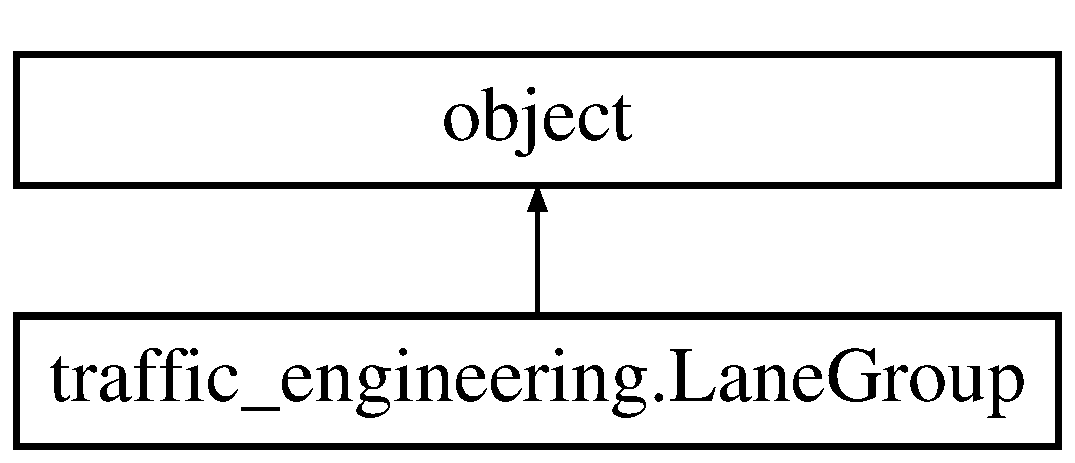
\includegraphics[height=2.000000cm]{classtraffic__engineering_1_1LaneGroup}
\end{center}
\end{figure}
\subsubsection*{Public Member Functions}
\begin{DoxyCompactItemize}
\item 
def \hyperlink{classtraffic__engineering_1_1LaneGroup_a1ec9c2c27c59cbe3b94aec4cd4149c97}{\-\_\-\-\_\-init\-\_\-\-\_\-}
\item 
def \hyperlink{classtraffic__engineering_1_1LaneGroup_a7046c83964c96e8c5e619363e5f8102b}{get\-T\-V\-U\-Volume}
\item 
def \hyperlink{classtraffic__engineering_1_1LaneGroup_a169b990761b6ea56563b6135dd129e80}{get\-Charge}
\end{DoxyCompactItemize}
\subsubsection*{Public Attributes}
\begin{DoxyCompactItemize}
\item 
\hyperlink{classtraffic__engineering_1_1LaneGroup_a96479716a1b5a03f2176a728d73c28a5}{movements}
\item 
\hyperlink{classtraffic__engineering_1_1LaneGroup_ad0a5c0cd3bdf8c1c38860ea81f8d3b2e}{n\-Lanes}
\end{DoxyCompactItemize}


\subsubsection{Detailed Description}
\begin{DoxyVerb}Class that represents a group of mouvements\end{DoxyVerb}
 

\subsubsection{Constructor \& Destructor Documentation}
\hypertarget{classtraffic__engineering_1_1LaneGroup_a1ec9c2c27c59cbe3b94aec4cd4149c97}{\index{traffic\-\_\-engineering\-::\-Lane\-Group@{traffic\-\_\-engineering\-::\-Lane\-Group}!\-\_\-\-\_\-init\-\_\-\-\_\-@{\-\_\-\-\_\-init\-\_\-\-\_\-}}
\index{\-\_\-\-\_\-init\-\_\-\-\_\-@{\-\_\-\-\_\-init\-\_\-\-\_\-}!traffic_engineering::LaneGroup@{traffic\-\_\-engineering\-::\-Lane\-Group}}
\paragraph[{\-\_\-\-\_\-init\-\_\-\-\_\-}]{\setlength{\rightskip}{0pt plus 5cm}def traffic\-\_\-engineering.\-Lane\-Group.\-\_\-\-\_\-init\-\_\-\-\_\- (
\begin{DoxyParamCaption}
\item[{}]{self, }
\item[{}]{movements, }
\item[{}]{n\-Lanes}
\end{DoxyParamCaption}
)}}\label{classtraffic__engineering_1_1LaneGroup_a1ec9c2c27c59cbe3b94aec4cd4149c97}


\subsubsection{Member Function Documentation}
\hypertarget{classtraffic__engineering_1_1LaneGroup_a169b990761b6ea56563b6135dd129e80}{\index{traffic\-\_\-engineering\-::\-Lane\-Group@{traffic\-\_\-engineering\-::\-Lane\-Group}!get\-Charge@{get\-Charge}}
\index{get\-Charge@{get\-Charge}!traffic_engineering::LaneGroup@{traffic\-\_\-engineering\-::\-Lane\-Group}}
\paragraph[{get\-Charge}]{\setlength{\rightskip}{0pt plus 5cm}def traffic\-\_\-engineering.\-Lane\-Group.\-get\-Charge (
\begin{DoxyParamCaption}
\item[{}]{self, }
\item[{}]{saturation\-Volume}
\end{DoxyParamCaption}
)}}\label{classtraffic__engineering_1_1LaneGroup_a169b990761b6ea56563b6135dd129e80}


References traffic\-\_\-engineering.\-Intersection\-Movement.\-get\-T\-V\-U\-Volume(), traffic\-\_\-engineering.\-Lane\-Group.\-get\-T\-V\-U\-Volume(), traffic\-\_\-engineering.\-Volume.\-n\-Lanes, and traffic\-\_\-engineering.\-Lane\-Group.\-n\-Lanes.

\hypertarget{classtraffic__engineering_1_1LaneGroup_a7046c83964c96e8c5e619363e5f8102b}{\index{traffic\-\_\-engineering\-::\-Lane\-Group@{traffic\-\_\-engineering\-::\-Lane\-Group}!get\-T\-V\-U\-Volume@{get\-T\-V\-U\-Volume}}
\index{get\-T\-V\-U\-Volume@{get\-T\-V\-U\-Volume}!traffic_engineering::LaneGroup@{traffic\-\_\-engineering\-::\-Lane\-Group}}
\paragraph[{get\-T\-V\-U\-Volume}]{\setlength{\rightskip}{0pt plus 5cm}def traffic\-\_\-engineering.\-Lane\-Group.\-get\-T\-V\-U\-Volume (
\begin{DoxyParamCaption}
\item[{}]{self}
\end{DoxyParamCaption}
)}}\label{classtraffic__engineering_1_1LaneGroup_a7046c83964c96e8c5e619363e5f8102b}


References traffic\-\_\-engineering.\-Lane\-Group.\-movements.



\subsubsection{Member Data Documentation}
\hypertarget{classtraffic__engineering_1_1LaneGroup_a96479716a1b5a03f2176a728d73c28a5}{\index{traffic\-\_\-engineering\-::\-Lane\-Group@{traffic\-\_\-engineering\-::\-Lane\-Group}!movements@{movements}}
\index{movements@{movements}!traffic_engineering::LaneGroup@{traffic\-\_\-engineering\-::\-Lane\-Group}}
\paragraph[{movements}]{\setlength{\rightskip}{0pt plus 5cm}traffic\-\_\-engineering.\-Lane\-Group.\-movements}}\label{classtraffic__engineering_1_1LaneGroup_a96479716a1b5a03f2176a728d73c28a5}
\hypertarget{classtraffic__engineering_1_1LaneGroup_ad0a5c0cd3bdf8c1c38860ea81f8d3b2e}{\index{traffic\-\_\-engineering\-::\-Lane\-Group@{traffic\-\_\-engineering\-::\-Lane\-Group}!n\-Lanes@{n\-Lanes}}
\index{n\-Lanes@{n\-Lanes}!traffic_engineering::LaneGroup@{traffic\-\_\-engineering\-::\-Lane\-Group}}
\paragraph[{n\-Lanes}]{\setlength{\rightskip}{0pt plus 5cm}traffic\-\_\-engineering.\-Lane\-Group.\-n\-Lanes}}\label{classtraffic__engineering_1_1LaneGroup_ad0a5c0cd3bdf8c1c38860ea81f8d3b2e}


The documentation for this class was generated from the following file\-:\begin{DoxyCompactItemize}
\item 
python/\hyperlink{traffic__engineering_8py}{traffic\-\_\-engineering.\-py}\end{DoxyCompactItemize}

\hypertarget{classindicators_1_1LCSS}{\subsection{indicators.\-L\-C\-S\-S Class Reference}
\label{classindicators_1_1LCSS}\index{indicators.\-L\-C\-S\-S@{indicators.\-L\-C\-S\-S}}
}
Inheritance diagram for indicators.\-L\-C\-S\-S\-:\begin{figure}[H]
\begin{center}
\leavevmode
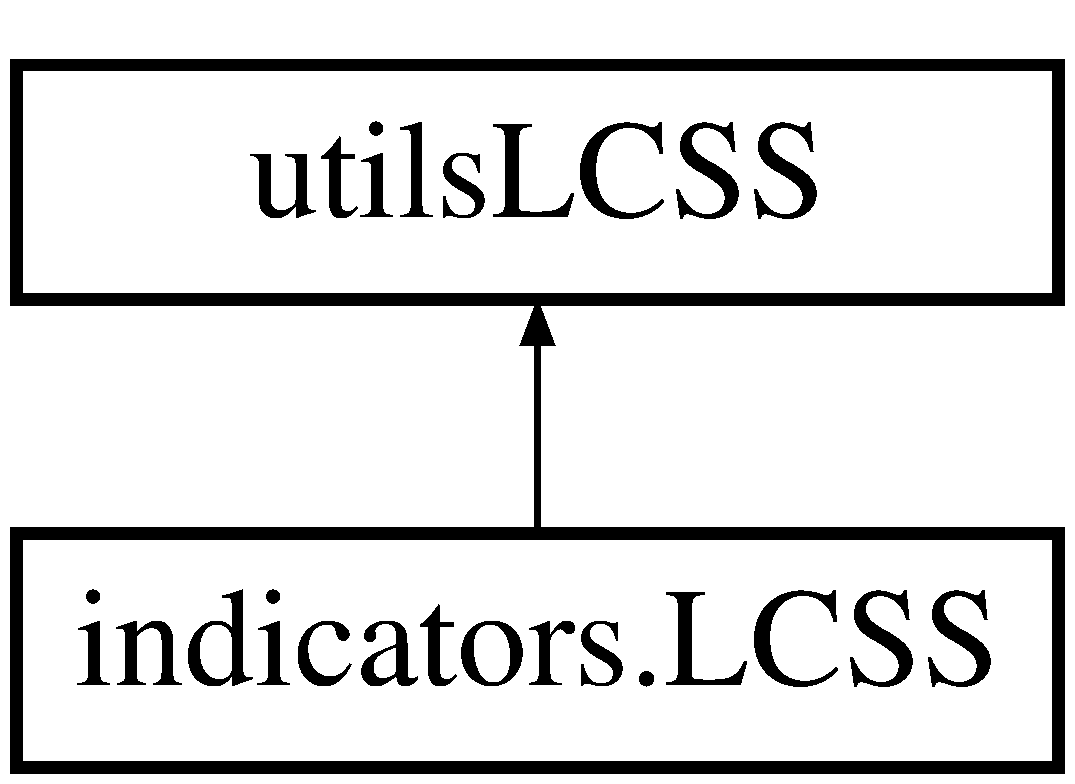
\includegraphics[height=2.000000cm]{classindicators_1_1LCSS}
\end{center}
\end{figure}
\subsubsection*{Public Member Functions}
\begin{DoxyCompactItemize}
\item 
def \hyperlink{classindicators_1_1LCSS_a17d13ad8eb307a864f475b388e05c9e0}{\-\_\-\-\_\-init\-\_\-\-\_\-}
\item 
def \hyperlink{classindicators_1_1LCSS_a4b79257cd0e5c8383db08553faa0853b}{check\-Indicator}
\item 
def \hyperlink{classindicators_1_1LCSS_a644d5b15a07d84756e32ab13cf19907d}{compute}
\item 
def \hyperlink{classindicators_1_1LCSS_af89b68438ef7f2040016f5e52d8415bd}{compute\-Normalized}
\item 
def \hyperlink{classindicators_1_1LCSS_acadd8297a0e637f11c85eebca941c4b8}{compute\-Distance}
\end{DoxyCompactItemize}
\subsubsection*{Public Attributes}
\begin{DoxyCompactItemize}
\item 
\hyperlink{classindicators_1_1LCSS_a64d8820e7557d7e6ad202de0b9a5ca43}{min\-Length}
\end{DoxyCompactItemize}


\subsubsection{Detailed Description}
\begin{DoxyVerb}Adapted LCSS class for indicators, same pattern\end{DoxyVerb}
 

\subsubsection{Constructor \& Destructor Documentation}
\hypertarget{classindicators_1_1LCSS_a17d13ad8eb307a864f475b388e05c9e0}{\index{indicators\-::\-L\-C\-S\-S@{indicators\-::\-L\-C\-S\-S}!\-\_\-\-\_\-init\-\_\-\-\_\-@{\-\_\-\-\_\-init\-\_\-\-\_\-}}
\index{\-\_\-\-\_\-init\-\_\-\-\_\-@{\-\_\-\-\_\-init\-\_\-\-\_\-}!indicators::LCSS@{indicators\-::\-L\-C\-S\-S}}
\paragraph[{\-\_\-\-\_\-init\-\_\-\-\_\-}]{\setlength{\rightskip}{0pt plus 5cm}def indicators.\-L\-C\-S\-S.\-\_\-\-\_\-init\-\_\-\-\_\- (
\begin{DoxyParamCaption}
\item[{}]{self, }
\item[{}]{similarity\-Func, }
\item[{}]{delta = {\ttfamily float('inf')}, }
\item[{}]{min\-Length = {\ttfamily 0}, }
\item[{}]{aligned = {\ttfamily False}, }
\item[{}]{length\-Func = {\ttfamily min}}
\end{DoxyParamCaption}
)}}\label{classindicators_1_1LCSS_a17d13ad8eb307a864f475b388e05c9e0}


\subsubsection{Member Function Documentation}
\hypertarget{classindicators_1_1LCSS_a4b79257cd0e5c8383db08553faa0853b}{\index{indicators\-::\-L\-C\-S\-S@{indicators\-::\-L\-C\-S\-S}!check\-Indicator@{check\-Indicator}}
\index{check\-Indicator@{check\-Indicator}!indicators::LCSS@{indicators\-::\-L\-C\-S\-S}}
\paragraph[{check\-Indicator}]{\setlength{\rightskip}{0pt plus 5cm}def indicators.\-L\-C\-S\-S.\-check\-Indicator (
\begin{DoxyParamCaption}
\item[{}]{self, }
\item[{}]{indicator}
\end{DoxyParamCaption}
)}}\label{classindicators_1_1LCSS_a4b79257cd0e5c8383db08553faa0853b}


References indicators.\-L\-C\-S\-S.\-min\-Length.

\hypertarget{classindicators_1_1LCSS_a644d5b15a07d84756e32ab13cf19907d}{\index{indicators\-::\-L\-C\-S\-S@{indicators\-::\-L\-C\-S\-S}!compute@{compute}}
\index{compute@{compute}!indicators::LCSS@{indicators\-::\-L\-C\-S\-S}}
\paragraph[{compute}]{\setlength{\rightskip}{0pt plus 5cm}def indicators.\-L\-C\-S\-S.\-compute (
\begin{DoxyParamCaption}
\item[{}]{self, }
\item[{}]{indicator1, }
\item[{}]{indicator2, }
\item[{}]{compute\-Sub\-Sequence = {\ttfamily False}}
\end{DoxyParamCaption}
)}}\label{classindicators_1_1LCSS_a644d5b15a07d84756e32ab13cf19907d}


References indicators.\-L\-C\-S\-S.\-check\-Indicator().

\hypertarget{classindicators_1_1LCSS_acadd8297a0e637f11c85eebca941c4b8}{\index{indicators\-::\-L\-C\-S\-S@{indicators\-::\-L\-C\-S\-S}!compute\-Distance@{compute\-Distance}}
\index{compute\-Distance@{compute\-Distance}!indicators::LCSS@{indicators\-::\-L\-C\-S\-S}}
\paragraph[{compute\-Distance}]{\setlength{\rightskip}{0pt plus 5cm}def indicators.\-L\-C\-S\-S.\-compute\-Distance (
\begin{DoxyParamCaption}
\item[{}]{self, }
\item[{}]{indicator1, }
\item[{}]{indicator2, }
\item[{}]{compute\-Sub\-Sequence = {\ttfamily False}}
\end{DoxyParamCaption}
)}}\label{classindicators_1_1LCSS_acadd8297a0e637f11c85eebca941c4b8}


References indicators.\-L\-C\-S\-S.\-check\-Indicator().

\hypertarget{classindicators_1_1LCSS_af89b68438ef7f2040016f5e52d8415bd}{\index{indicators\-::\-L\-C\-S\-S@{indicators\-::\-L\-C\-S\-S}!compute\-Normalized@{compute\-Normalized}}
\index{compute\-Normalized@{compute\-Normalized}!indicators::LCSS@{indicators\-::\-L\-C\-S\-S}}
\paragraph[{compute\-Normalized}]{\setlength{\rightskip}{0pt plus 5cm}def indicators.\-L\-C\-S\-S.\-compute\-Normalized (
\begin{DoxyParamCaption}
\item[{}]{self, }
\item[{}]{indicator1, }
\item[{}]{indicator2, }
\item[{}]{compute\-Sub\-Sequence = {\ttfamily False}}
\end{DoxyParamCaption}
)}}\label{classindicators_1_1LCSS_af89b68438ef7f2040016f5e52d8415bd}


References indicators.\-L\-C\-S\-S.\-check\-Indicator().



\subsubsection{Member Data Documentation}
\hypertarget{classindicators_1_1LCSS_a64d8820e7557d7e6ad202de0b9a5ca43}{\index{indicators\-::\-L\-C\-S\-S@{indicators\-::\-L\-C\-S\-S}!min\-Length@{min\-Length}}
\index{min\-Length@{min\-Length}!indicators::LCSS@{indicators\-::\-L\-C\-S\-S}}
\paragraph[{min\-Length}]{\setlength{\rightskip}{0pt plus 5cm}indicators.\-L\-C\-S\-S.\-min\-Length}}\label{classindicators_1_1LCSS_a64d8820e7557d7e6ad202de0b9a5ca43}


The documentation for this class was generated from the following file\-:\begin{DoxyCompactItemize}
\item 
python/\hyperlink{indicators_8py}{indicators.\-py}\end{DoxyCompactItemize}

\hypertarget{classpavement_1_1MarkingTest}{\subsection{pavement.\-Marking\-Test Class Reference}
\label{classpavement_1_1MarkingTest}\index{pavement.\-Marking\-Test@{pavement.\-Marking\-Test}}
}
Inheritance diagram for pavement.\-Marking\-Test\-:\begin{figure}[H]
\begin{center}
\leavevmode
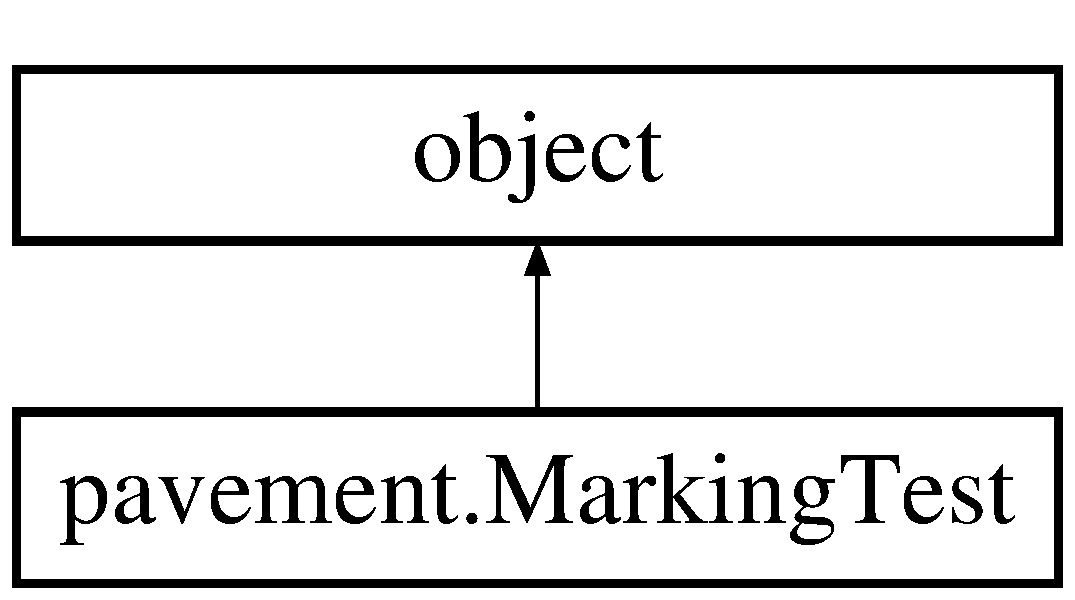
\includegraphics[height=2.000000cm]{classpavement_1_1MarkingTest}
\end{center}
\end{figure}
\subsubsection*{Public Member Functions}
\begin{DoxyCompactItemize}
\item 
def \hyperlink{classpavement_1_1MarkingTest_af7c408fcf3d5acf2ccf8ba17a68a75fd}{\-\_\-\-\_\-init\-\_\-\-\_\-}
\item 
def \hyperlink{classpavement_1_1MarkingTest_a2be83971e50867810b73d987f349f8b4}{get\-Site}
\item 
def \hyperlink{classpavement_1_1MarkingTest_aef5ec08883921f794e9409fc630a45e7}{get\-Test\-Attributes}
\item 
def \hyperlink{classpavement_1_1MarkingTest_a67a6a94c0bae15e6578ec18fb0fe3718}{plot}
\item 
def \hyperlink{classpavement_1_1MarkingTest_acd1a2b8a42d620ce628edef3b9bb73d3}{get\-Marking\-Measures}
\item 
def \hyperlink{classpavement_1_1MarkingTest_a2c66d4cd8fd42e55858dbcfcaccae92d}{plot\-Marking\-Measures}
\item 
def \hyperlink{classpavement_1_1MarkingTest_a01019e00a695160ca874811217ef42e9}{compute\-Marking\-Measure\-Variations}
\end{DoxyCompactItemize}
\subsubsection*{Public Attributes}
\begin{DoxyCompactItemize}
\item 
\hyperlink{classpavement_1_1MarkingTest_abbf2515122d9e6109429ed947edd98a4}{id}
\item 
\hyperlink{classpavement_1_1MarkingTest_a03f712cbf2f964a28e9eac685c480df8}{painting\-Date}
\item 
\hyperlink{classpavement_1_1MarkingTest_a812f9cf99f25212085a32db7b6565d74}{painting\-Type}
\item 
\hyperlink{classpavement_1_1MarkingTest_af4addf42878c5871635abcefc09aa967}{color}
\item 
\hyperlink{classpavement_1_1MarkingTest_ae49e22b6ecfa4c22f10ad0c22420a24d}{data}
\item 
\hyperlink{classpavement_1_1MarkingTest_a145264f1dd1b2b85fe254403c2646eb9}{n\-Measures}
\end{DoxyCompactItemize}


\subsubsection{Detailed Description}
\begin{DoxyVerb}class for a test site for a given product

including the series of measurements over the years\end{DoxyVerb}
 

\subsubsection{Constructor \& Destructor Documentation}
\hypertarget{classpavement_1_1MarkingTest_af7c408fcf3d5acf2ccf8ba17a68a75fd}{\index{pavement\-::\-Marking\-Test@{pavement\-::\-Marking\-Test}!\-\_\-\-\_\-init\-\_\-\-\_\-@{\-\_\-\-\_\-init\-\_\-\-\_\-}}
\index{\-\_\-\-\_\-init\-\_\-\-\_\-@{\-\_\-\-\_\-init\-\_\-\-\_\-}!pavement::MarkingTest@{pavement\-::\-Marking\-Test}}
\paragraph[{\-\_\-\-\_\-init\-\_\-\-\_\-}]{\setlength{\rightskip}{0pt plus 5cm}def pavement.\-Marking\-Test.\-\_\-\-\_\-init\-\_\-\-\_\- (
\begin{DoxyParamCaption}
\item[{}]{self, }
\item[{}]{\-\_\-id, }
\item[{}]{painting\-Date, }
\item[{}]{painting\-Type, }
\item[{}]{color, }
\item[{}]{data}
\end{DoxyParamCaption}
)}}\label{classpavement_1_1MarkingTest_af7c408fcf3d5acf2ccf8ba17a68a75fd}


\subsubsection{Member Function Documentation}
\hypertarget{classpavement_1_1MarkingTest_a01019e00a695160ca874811217ef42e9}{\index{pavement\-::\-Marking\-Test@{pavement\-::\-Marking\-Test}!compute\-Marking\-Measure\-Variations@{compute\-Marking\-Measure\-Variations}}
\index{compute\-Marking\-Measure\-Variations@{compute\-Marking\-Measure\-Variations}!pavement::MarkingTest@{pavement\-::\-Marking\-Test}}
\paragraph[{compute\-Marking\-Measure\-Variations}]{\setlength{\rightskip}{0pt plus 5cm}def pavement.\-Marking\-Test.\-compute\-Marking\-Measure\-Variations (
\begin{DoxyParamCaption}
\item[{}]{self, }
\item[{}]{data\-Label, }
\item[{}]{lane\-Positions, }
\item[{}]{weather\-Data, }
\item[{}]{snow\-Threshold, }
\item[{}]{weather\-Data\-Type = {\ttfamily 'ec'}, }
\item[{}]{min\-Proportion\-Measures = {\ttfamily 0.}}
\end{DoxyParamCaption}
)}}\label{classpavement_1_1MarkingTest_a01019e00a695160ca874811217ef42e9}
\begin{DoxyVerb}Computes for each successive measurement
lanePositions = None
measure variation, initial measure, time duration, weather indicators

TODO if measurements per lane, add a variable for lane position (position1 to 6)
lanePositions = list of integers (range(1,7))
measure variation, initial measure, time duration, lane position1, weather indicators
measure variation, initial measure, time duration, lane position2, weather indicators
...\end{DoxyVerb}
 

References pavement.\-R\-T\-S\-S.\-data, pavement.\-Marking\-Test.\-data, and pavement.\-weather\-Indicators().

\hypertarget{classpavement_1_1MarkingTest_acd1a2b8a42d620ce628edef3b9bb73d3}{\index{pavement\-::\-Marking\-Test@{pavement\-::\-Marking\-Test}!get\-Marking\-Measures@{get\-Marking\-Measures}}
\index{get\-Marking\-Measures@{get\-Marking\-Measures}!pavement::MarkingTest@{pavement\-::\-Marking\-Test}}
\paragraph[{get\-Marking\-Measures}]{\setlength{\rightskip}{0pt plus 5cm}def pavement.\-Marking\-Test.\-get\-Marking\-Measures (
\begin{DoxyParamCaption}
\item[{}]{self, }
\item[{}]{data\-Label}
\end{DoxyParamCaption}
)}}\label{classpavement_1_1MarkingTest_acd1a2b8a42d620ce628edef3b9bb73d3}


References pavement.\-R\-T\-S\-S.\-data, and pavement.\-Marking\-Test.\-data.

\hypertarget{classpavement_1_1MarkingTest_a2be83971e50867810b73d987f349f8b4}{\index{pavement\-::\-Marking\-Test@{pavement\-::\-Marking\-Test}!get\-Site@{get\-Site}}
\index{get\-Site@{get\-Site}!pavement::MarkingTest@{pavement\-::\-Marking\-Test}}
\paragraph[{get\-Site}]{\setlength{\rightskip}{0pt plus 5cm}def pavement.\-Marking\-Test.\-get\-Site (
\begin{DoxyParamCaption}
\item[{}]{self}
\end{DoxyParamCaption}
)}}\label{classpavement_1_1MarkingTest_a2be83971e50867810b73d987f349f8b4}


References pavement.\-R\-T\-S\-S.\-id, and pavement.\-Marking\-Test.\-id.

\hypertarget{classpavement_1_1MarkingTest_aef5ec08883921f794e9409fc630a45e7}{\index{pavement\-::\-Marking\-Test@{pavement\-::\-Marking\-Test}!get\-Test\-Attributes@{get\-Test\-Attributes}}
\index{get\-Test\-Attributes@{get\-Test\-Attributes}!pavement::MarkingTest@{pavement\-::\-Marking\-Test}}
\paragraph[{get\-Test\-Attributes}]{\setlength{\rightskip}{0pt plus 5cm}def pavement.\-Marking\-Test.\-get\-Test\-Attributes (
\begin{DoxyParamCaption}
\item[{}]{self}
\end{DoxyParamCaption}
)}}\label{classpavement_1_1MarkingTest_aef5ec08883921f794e9409fc630a45e7}


References Colors.\-color, pavement.\-Marking\-Test.\-color, and pavement.\-Marking\-Test.\-painting\-Type.

\hypertarget{classpavement_1_1MarkingTest_a67a6a94c0bae15e6578ec18fb0fe3718}{\index{pavement\-::\-Marking\-Test@{pavement\-::\-Marking\-Test}!plot@{plot}}
\index{plot@{plot}!pavement::MarkingTest@{pavement\-::\-Marking\-Test}}
\paragraph[{plot}]{\setlength{\rightskip}{0pt plus 5cm}def pavement.\-Marking\-Test.\-plot (
\begin{DoxyParamCaption}
\item[{}]{self, }
\item[{}]{measure, }
\item[{}]{options = {\ttfamily 'o'}, }
\item[{}]{day\-Ratio = {\ttfamily 1.}, }
\item[{}]{kwargs}
\end{DoxyParamCaption}
)}}\label{classpavement_1_1MarkingTest_a67a6a94c0bae15e6578ec18fb0fe3718}


References pavement.\-R\-T\-S\-S.\-data, and pavement.\-Marking\-Test.\-data.

\hypertarget{classpavement_1_1MarkingTest_a2c66d4cd8fd42e55858dbcfcaccae92d}{\index{pavement\-::\-Marking\-Test@{pavement\-::\-Marking\-Test}!plot\-Marking\-Measures@{plot\-Marking\-Measures}}
\index{plot\-Marking\-Measures@{plot\-Marking\-Measures}!pavement::MarkingTest@{pavement\-::\-Marking\-Test}}
\paragraph[{plot\-Marking\-Measures}]{\setlength{\rightskip}{0pt plus 5cm}def pavement.\-Marking\-Test.\-plot\-Marking\-Measures (
\begin{DoxyParamCaption}
\item[{}]{self, }
\item[{}]{measure, }
\item[{}]{options = {\ttfamily 'o'}, }
\item[{}]{day\-Ratio = {\ttfamily 1.}, }
\item[{}]{kwargs}
\end{DoxyParamCaption}
)}}\label{classpavement_1_1MarkingTest_a2c66d4cd8fd42e55858dbcfcaccae92d}


References ml.\-Centroid.\-plot(), indicators.\-Temporal\-Indicator.\-plot(), events.\-Interaction.\-plot(), moving.\-Point.\-plot(), pavement.\-Marking\-Test.\-plot(), moving.\-Flow\-Vector.\-plot(), moving.\-Trajectory.\-plot(), and moving.\-Moving\-Object.\-plot().



\subsubsection{Member Data Documentation}
\hypertarget{classpavement_1_1MarkingTest_af4addf42878c5871635abcefc09aa967}{\index{pavement\-::\-Marking\-Test@{pavement\-::\-Marking\-Test}!color@{color}}
\index{color@{color}!pavement::MarkingTest@{pavement\-::\-Marking\-Test}}
\paragraph[{color}]{\setlength{\rightskip}{0pt plus 5cm}pavement.\-Marking\-Test.\-color}}\label{classpavement_1_1MarkingTest_af4addf42878c5871635abcefc09aa967}
\hypertarget{classpavement_1_1MarkingTest_ae49e22b6ecfa4c22f10ad0c22420a24d}{\index{pavement\-::\-Marking\-Test@{pavement\-::\-Marking\-Test}!data@{data}}
\index{data@{data}!pavement::MarkingTest@{pavement\-::\-Marking\-Test}}
\paragraph[{data}]{\setlength{\rightskip}{0pt plus 5cm}pavement.\-Marking\-Test.\-data}}\label{classpavement_1_1MarkingTest_ae49e22b6ecfa4c22f10ad0c22420a24d}
\hypertarget{classpavement_1_1MarkingTest_abbf2515122d9e6109429ed947edd98a4}{\index{pavement\-::\-Marking\-Test@{pavement\-::\-Marking\-Test}!id@{id}}
\index{id@{id}!pavement::MarkingTest@{pavement\-::\-Marking\-Test}}
\paragraph[{id}]{\setlength{\rightskip}{0pt plus 5cm}pavement.\-Marking\-Test.\-id}}\label{classpavement_1_1MarkingTest_abbf2515122d9e6109429ed947edd98a4}
\hypertarget{classpavement_1_1MarkingTest_a145264f1dd1b2b85fe254403c2646eb9}{\index{pavement\-::\-Marking\-Test@{pavement\-::\-Marking\-Test}!n\-Measures@{n\-Measures}}
\index{n\-Measures@{n\-Measures}!pavement::MarkingTest@{pavement\-::\-Marking\-Test}}
\paragraph[{n\-Measures}]{\setlength{\rightskip}{0pt plus 5cm}pavement.\-Marking\-Test.\-n\-Measures}}\label{classpavement_1_1MarkingTest_a145264f1dd1b2b85fe254403c2646eb9}
\hypertarget{classpavement_1_1MarkingTest_a03f712cbf2f964a28e9eac685c480df8}{\index{pavement\-::\-Marking\-Test@{pavement\-::\-Marking\-Test}!painting\-Date@{painting\-Date}}
\index{painting\-Date@{painting\-Date}!pavement::MarkingTest@{pavement\-::\-Marking\-Test}}
\paragraph[{painting\-Date}]{\setlength{\rightskip}{0pt plus 5cm}pavement.\-Marking\-Test.\-painting\-Date}}\label{classpavement_1_1MarkingTest_a03f712cbf2f964a28e9eac685c480df8}
\hypertarget{classpavement_1_1MarkingTest_a812f9cf99f25212085a32db7b6565d74}{\index{pavement\-::\-Marking\-Test@{pavement\-::\-Marking\-Test}!painting\-Type@{painting\-Type}}
\index{painting\-Type@{painting\-Type}!pavement::MarkingTest@{pavement\-::\-Marking\-Test}}
\paragraph[{painting\-Type}]{\setlength{\rightskip}{0pt plus 5cm}pavement.\-Marking\-Test.\-painting\-Type}}\label{classpavement_1_1MarkingTest_a812f9cf99f25212085a32db7b6565d74}


The documentation for this class was generated from the following file\-:\begin{DoxyCompactItemize}
\item 
python/\hyperlink{pavement_8py}{pavement.\-py}\end{DoxyCompactItemize}

\hypertarget{classCatch_1_1MethodTestCase}{\subsection{Catch\-:\-:Method\-Test\-Case$<$ C $>$ Class Template Reference}
\label{classCatch_1_1MethodTestCase}\index{Catch\-::\-Method\-Test\-Case$<$ C $>$@{Catch\-::\-Method\-Test\-Case$<$ C $>$}}
}


{\ttfamily \#include $<$catch.\-hpp$>$}

Inheritance diagram for Catch\-:\-:Method\-Test\-Case$<$ C $>$\-:\begin{figure}[H]
\begin{center}
\leavevmode
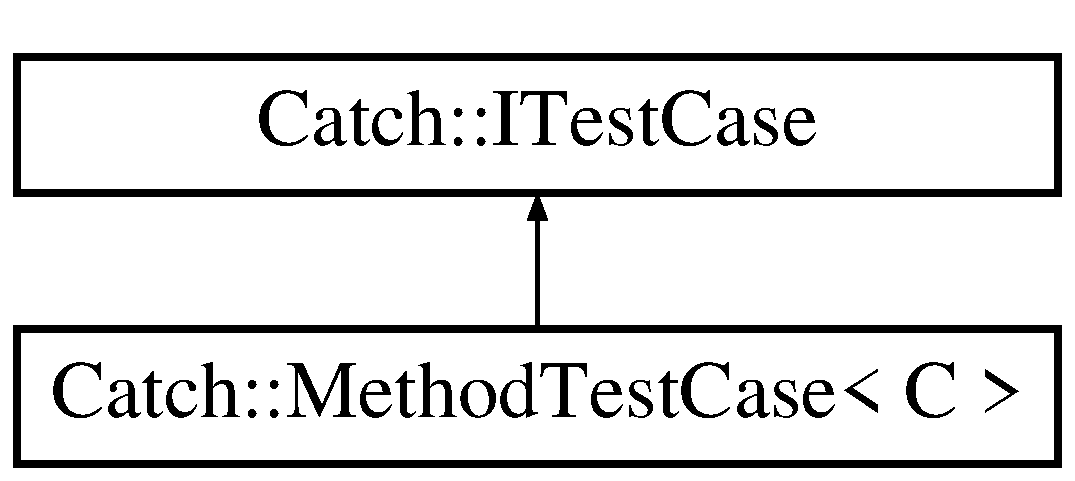
\includegraphics[height=2.000000cm]{classCatch_1_1MethodTestCase}
\end{center}
\end{figure}
\subsubsection*{Public Member Functions}
\begin{DoxyCompactItemize}
\item 
\hyperlink{classCatch_1_1MethodTestCase_a7b043b85dae371358255dd9dc6582e7b}{Method\-Test\-Case} (void(C\-::$\ast$method)())
\item 
virtual void \hyperlink{classCatch_1_1MethodTestCase_a39cc4b760dd71adc3f7550bc1e7eb697}{invoke} () const 
\item 
virtual \hyperlink{structCatch_1_1ITestCase}{I\-Test\-Case} $\ast$ \hyperlink{classCatch_1_1MethodTestCase_a11448e37336915c7f93d470b4c517961}{clone} () const 
\item 
virtual bool \hyperlink{classCatch_1_1MethodTestCase_a78295dacec5d279e6ea312c6af9aebb0}{operator==} (const \hyperlink{structCatch_1_1ITestCase}{I\-Test\-Case} \&other) const 
\item 
virtual bool \hyperlink{classCatch_1_1MethodTestCase_ac411bdeb5057d7e32ef64e1287debbef}{operator$<$} (const \hyperlink{structCatch_1_1ITestCase}{I\-Test\-Case} \&other) const 
\end{DoxyCompactItemize}


\subsubsection{Constructor \& Destructor Documentation}
\hypertarget{classCatch_1_1MethodTestCase_a7b043b85dae371358255dd9dc6582e7b}{\index{Catch\-::\-Method\-Test\-Case@{Catch\-::\-Method\-Test\-Case}!Method\-Test\-Case@{Method\-Test\-Case}}
\index{Method\-Test\-Case@{Method\-Test\-Case}!Catch::MethodTestCase@{Catch\-::\-Method\-Test\-Case}}
\paragraph[{Method\-Test\-Case}]{\setlength{\rightskip}{0pt plus 5cm}template$<$typename C $>$ {\bf Catch\-::\-Method\-Test\-Case}$<$ C $>$\-::{\bf Method\-Test\-Case} (
\begin{DoxyParamCaption}
\item[{void(C\-::$\ast$)()}]{method}
\end{DoxyParamCaption}
)\hspace{0.3cm}{\ttfamily [inline]}}}\label{classCatch_1_1MethodTestCase_a7b043b85dae371358255dd9dc6582e7b}


\subsubsection{Member Function Documentation}
\hypertarget{classCatch_1_1MethodTestCase_a11448e37336915c7f93d470b4c517961}{\index{Catch\-::\-Method\-Test\-Case@{Catch\-::\-Method\-Test\-Case}!clone@{clone}}
\index{clone@{clone}!Catch::MethodTestCase@{Catch\-::\-Method\-Test\-Case}}
\paragraph[{clone}]{\setlength{\rightskip}{0pt plus 5cm}template$<$typename C $>$ virtual {\bf I\-Test\-Case}$\ast$ {\bf Catch\-::\-Method\-Test\-Case}$<$ C $>$\-::clone (
\begin{DoxyParamCaption}
{}
\end{DoxyParamCaption}
) const\hspace{0.3cm}{\ttfamily [inline]}, {\ttfamily [virtual]}}}\label{classCatch_1_1MethodTestCase_a11448e37336915c7f93d470b4c517961}


Implements \hyperlink{structCatch_1_1ITestCase_af5307c170b81e94c14dc3d64ce598340}{Catch\-::\-I\-Test\-Case}.

\hypertarget{classCatch_1_1MethodTestCase_a39cc4b760dd71adc3f7550bc1e7eb697}{\index{Catch\-::\-Method\-Test\-Case@{Catch\-::\-Method\-Test\-Case}!invoke@{invoke}}
\index{invoke@{invoke}!Catch::MethodTestCase@{Catch\-::\-Method\-Test\-Case}}
\paragraph[{invoke}]{\setlength{\rightskip}{0pt plus 5cm}template$<$typename C $>$ virtual void {\bf Catch\-::\-Method\-Test\-Case}$<$ C $>$\-::invoke (
\begin{DoxyParamCaption}
{}
\end{DoxyParamCaption}
) const\hspace{0.3cm}{\ttfamily [inline]}, {\ttfamily [virtual]}}}\label{classCatch_1_1MethodTestCase_a39cc4b760dd71adc3f7550bc1e7eb697}


Implements \hyperlink{structCatch_1_1ITestCase_a678825e62e7c17297621cfeb65588c34}{Catch\-::\-I\-Test\-Case}.



References test-\/compute-\/object-\/position-\/from-\/features\-::obj.

\hypertarget{classCatch_1_1MethodTestCase_ac411bdeb5057d7e32ef64e1287debbef}{\index{Catch\-::\-Method\-Test\-Case@{Catch\-::\-Method\-Test\-Case}!operator$<$@{operator$<$}}
\index{operator$<$@{operator$<$}!Catch::MethodTestCase@{Catch\-::\-Method\-Test\-Case}}
\paragraph[{operator$<$}]{\setlength{\rightskip}{0pt plus 5cm}template$<$typename C $>$ virtual bool {\bf Catch\-::\-Method\-Test\-Case}$<$ C $>$\-::operator$<$ (
\begin{DoxyParamCaption}
\item[{const {\bf I\-Test\-Case} \&}]{other}
\end{DoxyParamCaption}
) const\hspace{0.3cm}{\ttfamily [inline]}, {\ttfamily [virtual]}}}\label{classCatch_1_1MethodTestCase_ac411bdeb5057d7e32ef64e1287debbef}


Implements \hyperlink{structCatch_1_1ITestCase_aae3e96da1a4494890326db813c010ddb}{Catch\-::\-I\-Test\-Case}.

\hypertarget{classCatch_1_1MethodTestCase_a78295dacec5d279e6ea312c6af9aebb0}{\index{Catch\-::\-Method\-Test\-Case@{Catch\-::\-Method\-Test\-Case}!operator==@{operator==}}
\index{operator==@{operator==}!Catch::MethodTestCase@{Catch\-::\-Method\-Test\-Case}}
\paragraph[{operator==}]{\setlength{\rightskip}{0pt plus 5cm}template$<$typename C $>$ virtual bool {\bf Catch\-::\-Method\-Test\-Case}$<$ C $>$\-::operator== (
\begin{DoxyParamCaption}
\item[{const {\bf I\-Test\-Case} \&}]{other}
\end{DoxyParamCaption}
) const\hspace{0.3cm}{\ttfamily [inline]}, {\ttfamily [virtual]}}}\label{classCatch_1_1MethodTestCase_a78295dacec5d279e6ea312c6af9aebb0}


Implements \hyperlink{structCatch_1_1ITestCase_a21ba9bd73bbf9c8e0384ed94d0f4cbb9}{Catch\-::\-I\-Test\-Case}.



The documentation for this class was generated from the following file\-:\begin{DoxyCompactItemize}
\item 
include/\hyperlink{catch_8hpp}{catch.\-hpp}\end{DoxyCompactItemize}

\hypertarget{classml_1_1Model}{\subsection{ml.\-Model Class Reference}
\label{classml_1_1Model}\index{ml.\-Model@{ml.\-Model}}
}
Inheritance diagram for ml.\-Model\-:\begin{figure}[H]
\begin{center}
\leavevmode
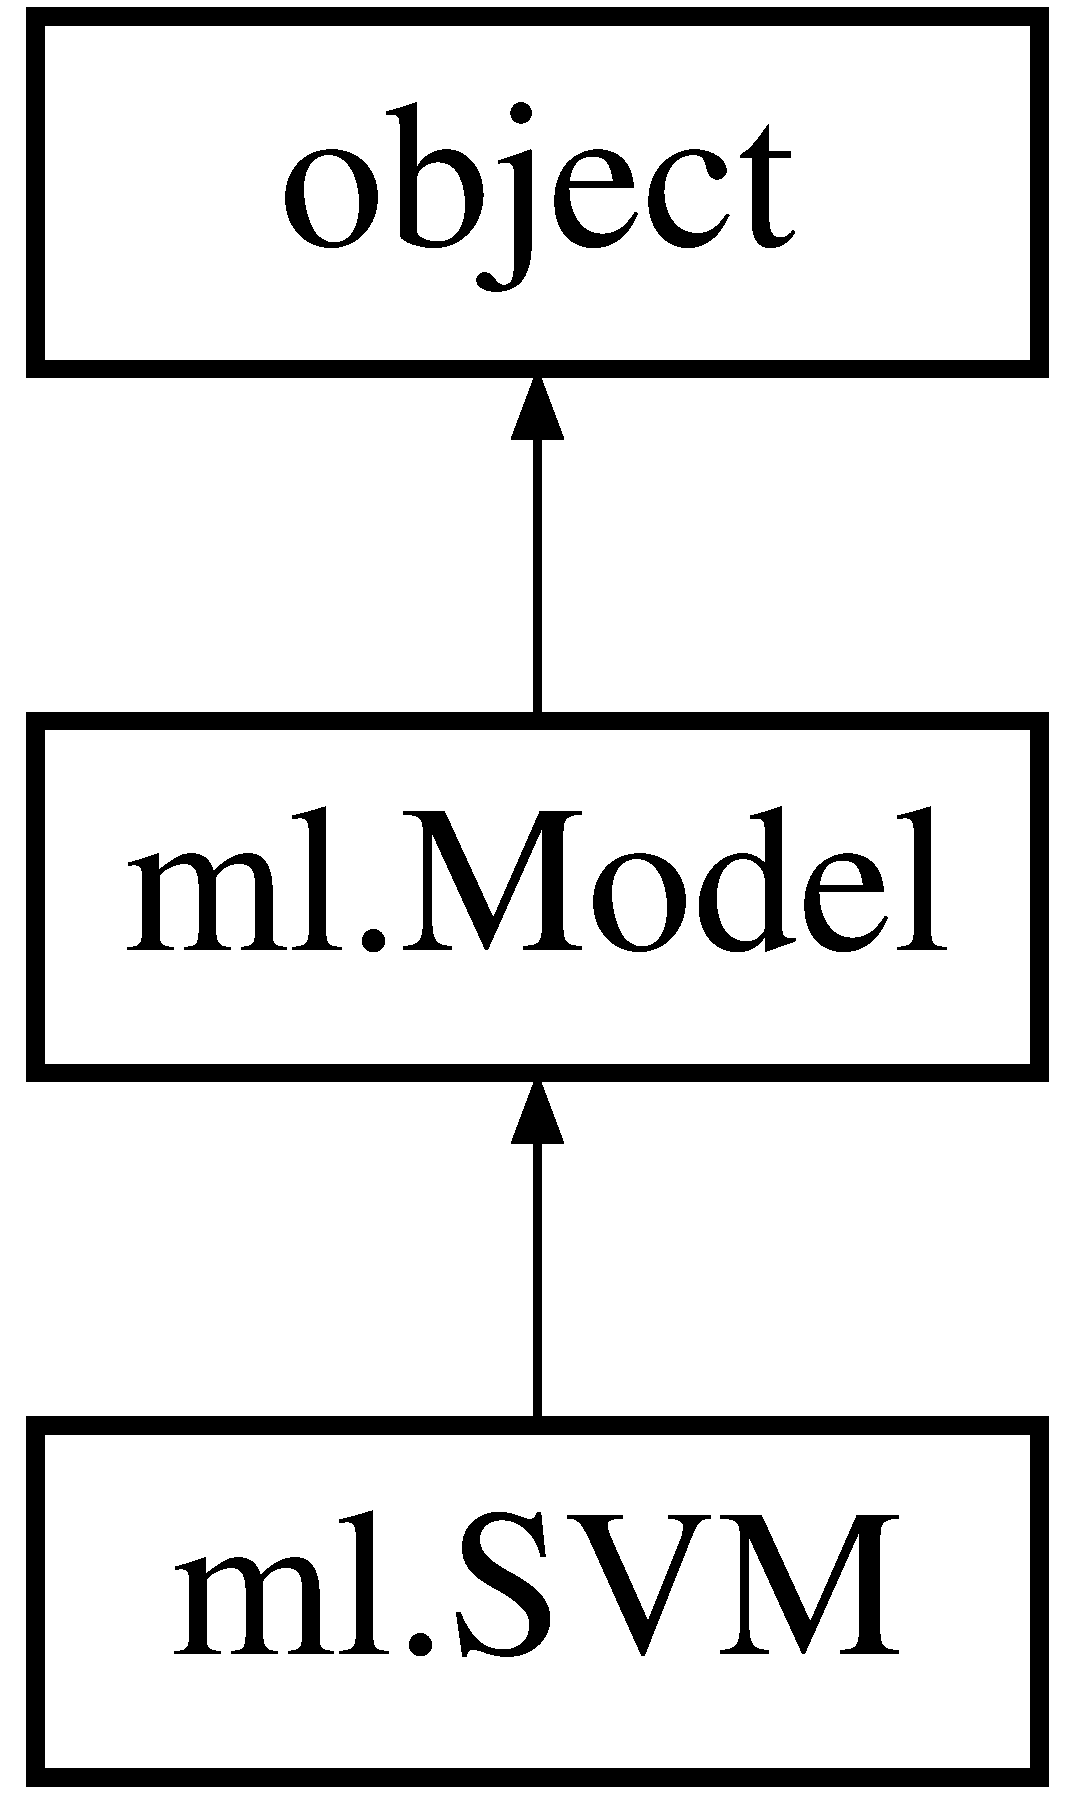
\includegraphics[height=3.000000cm]{classml_1_1Model}
\end{center}
\end{figure}
\subsubsection*{Public Member Functions}
\begin{DoxyCompactItemize}
\item 
def \hyperlink{classml_1_1Model_a4d2667369ddc5eabf6288365eb3f063c}{load}
\item 
def \hyperlink{classml_1_1Model_abca6fc59dd05209d31c1a4f545ebd598}{save}
\end{DoxyCompactItemize}


\subsubsection{Detailed Description}
\begin{DoxyVerb}Abstract class for loading/saving model\end{DoxyVerb}
 

\subsubsection{Member Function Documentation}
\hypertarget{classml_1_1Model_a4d2667369ddc5eabf6288365eb3f063c}{\index{ml\-::\-Model@{ml\-::\-Model}!load@{load}}
\index{load@{load}!ml::Model@{ml\-::\-Model}}
\paragraph[{load}]{\setlength{\rightskip}{0pt plus 5cm}def ml.\-Model.\-load (
\begin{DoxyParamCaption}
\item[{}]{self, }
\item[{}]{filename}
\end{DoxyParamCaption}
)}}\label{classml_1_1Model_a4d2667369ddc5eabf6288365eb3f063c}
\hypertarget{classml_1_1Model_abca6fc59dd05209d31c1a4f545ebd598}{\index{ml\-::\-Model@{ml\-::\-Model}!save@{save}}
\index{save@{save}!ml::Model@{ml\-::\-Model}}
\paragraph[{save}]{\setlength{\rightskip}{0pt plus 5cm}def ml.\-Model.\-save (
\begin{DoxyParamCaption}
\item[{}]{self, }
\item[{}]{filename}
\end{DoxyParamCaption}
)}}\label{classml_1_1Model_abca6fc59dd05209d31c1a4f545ebd598}


The documentation for this class was generated from the following file\-:\begin{DoxyCompactItemize}
\item 
python/\hyperlink{ml_8py}{ml.\-py}\end{DoxyCompactItemize}

\hypertarget{classmoving_1_1MovingObject}{\subsection{moving.\-Moving\-Object Class Reference}
\label{classmoving_1_1MovingObject}\index{moving.\-Moving\-Object@{moving.\-Moving\-Object}}
}
Inheritance diagram for moving.\-Moving\-Object\-:\begin{figure}[H]
\begin{center}
\leavevmode
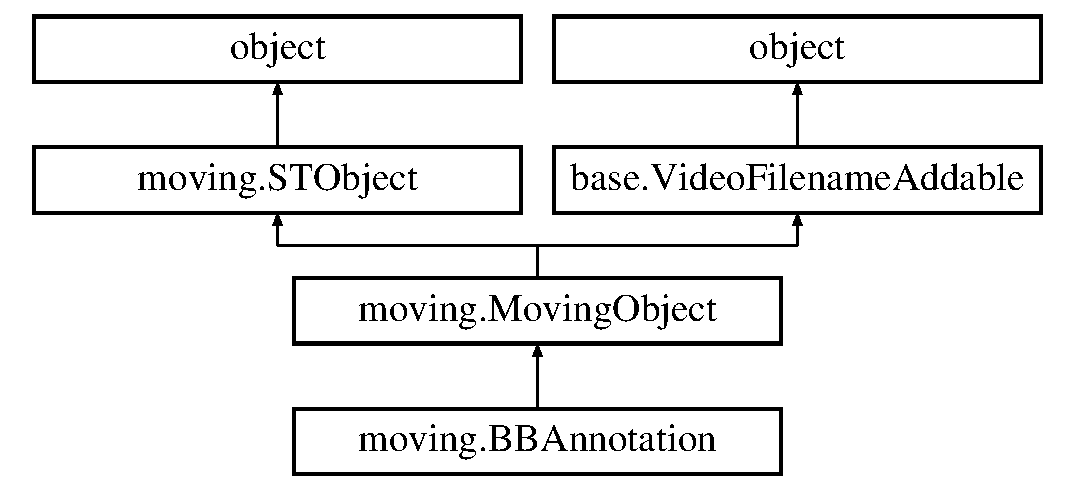
\includegraphics[height=4.000000cm]{classmoving_1_1MovingObject}
\end{center}
\end{figure}
\subsubsection*{Public Member Functions}
\begin{DoxyCompactItemize}
\item 
def \hyperlink{classmoving_1_1MovingObject_af5eb39b451844c27efa5a9afe6b442b0}{\-\_\-\-\_\-init\-\_\-\-\_\-}
\item 
def \hyperlink{classmoving_1_1MovingObject_a473f6a4eca09148db88439bd062a6802}{get\-Object\-In\-Time\-Interval}
\item 
def \hyperlink{classmoving_1_1MovingObject_a8725b010f6aa48dbc0b07b6714f15403}{get\-Objects\-In\-Mask}
\item 
def \hyperlink{classmoving_1_1MovingObject_a9c70c0c7dc3c938e70e6e4434f61b167}{get\-Positions}
\item 
def \hyperlink{classmoving_1_1MovingObject_a95c34c471a8f4f001e009c9ea5aed13b}{get\-Velocities}
\item 
def \hyperlink{classmoving_1_1MovingObject_a757700e17e0b75bb01e6b7324a3d5bdc}{get\-User\-Type}
\item 
def \hyperlink{classmoving_1_1MovingObject_aa589676e00e70ce8acafca9c3fa48150}{get\-Curvilinear\-Positions}
\item 
def \hyperlink{classmoving_1_1MovingObject_a8bff58ea20311713f7d08e1ed5482af6}{plot\-Curvilinear\-Positions}
\item 
def \hyperlink{classmoving_1_1MovingObject_a5b1caff7786c65076d09d79caec37f64}{set\-User\-Type}
\item 
def \hyperlink{classmoving_1_1MovingObject_aac41a9e6cf22cb70e5c9928322162e8b}{set\-Features}
\item 
def \hyperlink{classmoving_1_1MovingObject_a44af98d08a6ce2e6f09744abbf11e775}{get\-Features}
\item 
def \hyperlink{classmoving_1_1MovingObject_a971cfddbae99bd4ec26a1734f4e3cd4d}{has\-Features}
\item 
def \hyperlink{classmoving_1_1MovingObject_a398d9645b1ff68dc872f1d4bb7741ea3}{get\-Feature}
\item 
def \hyperlink{classmoving_1_1MovingObject_a70d454a13902eb10b7f5bde7af263c44}{get\-Feature\-Numbers}
\item 
def \hyperlink{classmoving_1_1MovingObject_aab0c83ba184a96a01e20a2e01ebc0afb}{get\-Speeds}
\item 
def \hyperlink{classmoving_1_1MovingObject_ac9edf3740c53ddc68d69fa6747b0c882}{get\-Speed\-Indicator}
\item 
def \hyperlink{classmoving_1_1MovingObject_ae47df2470c9fec917703400b5c962952}{get\-Position\-At}
\item 
def \hyperlink{classmoving_1_1MovingObject_a758f733dad0f9bf008cf45b89fe6063d}{get\-Velocity\-At}
\item 
def \hyperlink{classmoving_1_1MovingObject_a211e344ff77101e62a622013eadc71e4}{get\-Position\-At\-Instant}
\item 
def \hyperlink{classmoving_1_1MovingObject_a50f2867c8b6ba48f995739b0514233a9}{get\-Velocity\-At\-Instant}
\item 
def \hyperlink{classmoving_1_1MovingObject_aa343196bdaa82a5f77ebbfc27e44bc82}{get\-X\-Coordinates}
\item 
def \hyperlink{classmoving_1_1MovingObject_aba0e610ae2c0a8a205dadc9050fabc5d}{get\-Y\-Coordinates}
\item 
def \hyperlink{classmoving_1_1MovingObject_ac3f01327779af30047cc5157bb888978}{plot}
\item 
def \hyperlink{classmoving_1_1MovingObject_abadedb1af95d3b454c9bd93ceaeaa01c}{plot\-On\-World\-Image}
\item 
def \hyperlink{classmoving_1_1MovingObject_a64fd36dc48667b8210cc4c1a99a07338}{play}
\item 
def \hyperlink{classmoving_1_1MovingObject_aaf2dbfc97c3369654635449de3a14292}{speed\-Diagnostics}
\item 
def \hyperlink{classmoving_1_1MovingObject_a421d11edb5a6aca8cecacec5281c6989}{max\-Size}
\item 
def \hyperlink{classmoving_1_1MovingObject_a2fe41fc0d9a175e20490bd99ac400156}{set\-Routes}
\item 
def \hyperlink{classmoving_1_1MovingObject_ac58512c182f4c68fe27d5c959e9746b6}{get\-Instants\-Crossing\-Lane}
\item 
def \hyperlink{classmoving_1_1MovingObject_a4c784dd1df16736aaa6d0704e909adea}{predict\-Position}
\item 
def \hyperlink{classmoving_1_1MovingObject_afc87c0f8de37eb8d2802c331dad960ef}{project\-Curvilinear}
\item 
def \hyperlink{classmoving_1_1MovingObject_ad1de451e8476a36fd8fa83ba478f1906}{compute\-Smooth\-Trajectory}
\item 
def \hyperlink{classmoving_1_1MovingObject_af57a779bf124e557d2ebc522326e7d48}{classify\-User\-Type\-Speed\-Motorized}
\begin{DoxyCompactList}\small\item\em User Type Classification. \end{DoxyCompactList}\item 
def \hyperlink{classmoving_1_1MovingObject_a55eacbaf9483fc1b26079225079b8713}{classify\-User\-Type\-Speed}
\item 
def \hyperlink{classmoving_1_1MovingObject_a6cac8353066605307383fbebb2ad07b6}{init\-Classify\-User\-Type\-Ho\-G\-S\-V\-M}
\item 
def \hyperlink{classmoving_1_1MovingObject_a3c5b3b83b3854f211184ba7b113172f9}{classify\-User\-Type\-Ho\-G\-S\-V\-M\-At\-Instant}
\item 
def \hyperlink{classmoving_1_1MovingObject_ab6968b385f1c680030a23a26c46a5725}{classify\-User\-Type\-Ho\-G\-S\-V\-M}
\item 
def \hyperlink{classmoving_1_1MovingObject_a6fa5e07bb41a8c8d8d31d8059b9f43d4}{classify\-User\-Type\-Area}
\end{DoxyCompactItemize}
\subsubsection*{Static Public Member Functions}
\begin{DoxyCompactItemize}
\item 
def \hyperlink{classmoving_1_1MovingObject_aeee8f16c99b377c0d1b4fa1f4e321a1c}{generate}
\item 
def \hyperlink{classmoving_1_1MovingObject_aaa55660bfbfdf778b714f7b915947e93}{concatenate}
\item 
def \hyperlink{classmoving_1_1MovingObject_ab8c9203b44a17211bdcb41ec1d4a78b8}{min\-Max\-Distance}
\item 
def \hyperlink{classmoving_1_1MovingObject_a98dff92099bac9fd93779fa07f605f36}{distances}
\item 
def \hyperlink{classmoving_1_1MovingObject_a5386af60f864586a535978abe2353302}{min\-Distance}
\item 
def \hyperlink{classmoving_1_1MovingObject_a421db750d35abca7b07b70c9166677d5}{max\-Distance}
\item 
def \hyperlink{classmoving_1_1MovingObject_a2bfb4a35f6b50993c8e3fff36d39db0e}{compute\-P\-E\-T}
\item 
def \hyperlink{classmoving_1_1MovingObject_a347438cbdf8aa6f7e53108b7fc15a126}{collision\-Course\-Dot\-Product}
\item 
def \hyperlink{classmoving_1_1MovingObject_ac4c50f9830c66443fcdbd91d75d63e2b}{collision\-Course\-Cosine}
\end{DoxyCompactItemize}
\subsubsection*{Public Attributes}
\begin{DoxyCompactItemize}
\item 
\hyperlink{classmoving_1_1MovingObject_ab82e899e44b8d3c9a155da278d85b6ea}{positions}
\item 
\hyperlink{classmoving_1_1MovingObject_a705c214e02c9b4dab93d387044437923}{velocities}
\item 
\hyperlink{classmoving_1_1MovingObject_a35f9d997c873b53fa56ec29df5c422e7}{geometry}
\item 
\hyperlink{classmoving_1_1MovingObject_a4f078339d8175f616b3f167c6abf4d2d}{user\-Type}
\item 
\hyperlink{classmoving_1_1MovingObject_a06de9dfc5e3c0161167ea265d23d78a6}{features}
\item 
\hyperlink{classmoving_1_1MovingObject_afc473622764a5640a6b081d484051ae9}{projected\-Positions}
\item 
\hyperlink{classmoving_1_1MovingObject_a23e2a42b45ab136da5b02e9c8341fea1}{start\-Route\-I\-D}
\item 
\hyperlink{classmoving_1_1MovingObject_aad6902d0a0c16a55140b099aaccf6dd3}{end\-Route\-I\-D}
\item 
\hyperlink{classmoving_1_1MovingObject_a9f9ba9bddc49b8cf1bdaafb94a3f4bd5}{curvilinear\-Positions}
\item 
\hyperlink{classmoving_1_1MovingObject_a030eb07d7d94998b860272b4396ce5a4}{aggregated\-Speed}
\item 
\hyperlink{classmoving_1_1MovingObject_aa523c61416384436bff7bfe4d91074fd}{appearance\-Classifier}
\item 
\hyperlink{classmoving_1_1MovingObject_a25b52c7d2f777b62e565aed35a022e5c}{user\-Types}
\end{DoxyCompactItemize}


\subsubsection{Detailed Description}
\begin{DoxyVerb}Class for moving objects: a spatio-temporal object 
with a trajectory and a geometry (constant volume over time) 
and a usertype (e.g. road user) coded as a number (see userTypeNames)
\end{DoxyVerb}
 

\subsubsection{Constructor \& Destructor Documentation}
\hypertarget{classmoving_1_1MovingObject_af5eb39b451844c27efa5a9afe6b442b0}{\index{moving\-::\-Moving\-Object@{moving\-::\-Moving\-Object}!\-\_\-\-\_\-init\-\_\-\-\_\-@{\-\_\-\-\_\-init\-\_\-\-\_\-}}
\index{\-\_\-\-\_\-init\-\_\-\-\_\-@{\-\_\-\-\_\-init\-\_\-\-\_\-}!moving::MovingObject@{moving\-::\-Moving\-Object}}
\paragraph[{\-\_\-\-\_\-init\-\_\-\-\_\-}]{\setlength{\rightskip}{0pt plus 5cm}def moving.\-Moving\-Object.\-\_\-\-\_\-init\-\_\-\-\_\- (
\begin{DoxyParamCaption}
\item[{}]{self, }
\item[{}]{num = {\ttfamily None}, }
\item[{}]{time\-Interval = {\ttfamily None}, }
\item[{}]{positions = {\ttfamily None}, }
\item[{}]{velocities = {\ttfamily None}, }
\item[{}]{geometry = {\ttfamily None}, }
\item[{}]{user\-Type = {\ttfamily {\bf user\-Type2\-Num}\mbox{[}'unknown'\mbox{]}}}
\end{DoxyParamCaption}
)}}\label{classmoving_1_1MovingObject_af5eb39b451844c27efa5a9afe6b442b0}


\subsubsection{Member Function Documentation}
\hypertarget{classmoving_1_1MovingObject_a6fa5e07bb41a8c8d8d31d8059b9f43d4}{\index{moving\-::\-Moving\-Object@{moving\-::\-Moving\-Object}!classify\-User\-Type\-Area@{classify\-User\-Type\-Area}}
\index{classify\-User\-Type\-Area@{classify\-User\-Type\-Area}!moving::MovingObject@{moving\-::\-Moving\-Object}}
\paragraph[{classify\-User\-Type\-Area}]{\setlength{\rightskip}{0pt plus 5cm}def moving.\-Moving\-Object.\-classify\-User\-Type\-Area (
\begin{DoxyParamCaption}
\item[{}]{self, }
\item[{}]{areas, }
\item[{}]{homography}
\end{DoxyParamCaption}
)}}\label{classmoving_1_1MovingObject_a6fa5e07bb41a8c8d8d31d8059b9f43d4}
\begin{DoxyVerb}Classifies the object based on its location (projected to image space)
areas is a dictionary of matrix of the size of the image space 
for different road users possible locations, indexed by road user type names

TODO: areas could be a wrapper object with a contains method that would work for polygons and images (with wrapper class)
skip frames at beginning/end?\end{DoxyVerb}
 

References moving.\-Moving\-Object.\-projected\-Positions.

\hypertarget{classmoving_1_1MovingObject_ab6968b385f1c680030a23a26c46a5725}{\index{moving\-::\-Moving\-Object@{moving\-::\-Moving\-Object}!classify\-User\-Type\-Ho\-G\-S\-V\-M@{classify\-User\-Type\-Ho\-G\-S\-V\-M}}
\index{classify\-User\-Type\-Ho\-G\-S\-V\-M@{classify\-User\-Type\-Ho\-G\-S\-V\-M}!moving::MovingObject@{moving\-::\-Moving\-Object}}
\paragraph[{classify\-User\-Type\-Ho\-G\-S\-V\-M}]{\setlength{\rightskip}{0pt plus 5cm}def moving.\-Moving\-Object.\-classify\-User\-Type\-Ho\-G\-S\-V\-M (
\begin{DoxyParamCaption}
\item[{}]{self, }
\item[{}]{ped\-Bike\-Car\-S\-V\-M = {\ttfamily None}, }
\item[{}]{width = {\ttfamily 0}, }
\item[{}]{height = {\ttfamily 0}, }
\item[{}]{homography = {\ttfamily None}, }
\item[{}]{images = {\ttfamily None}, }
\item[{}]{bike\-Car\-S\-V\-M = {\ttfamily None}, }
\item[{}]{ped\-Bike\-Speed\-Treshold = {\ttfamily float('Inf')}, }
\item[{}]{bike\-Car\-Speed\-Threshold = {\ttfamily float('Inf')}, }
\item[{}]{min\-Speed\-Equiprobable = {\ttfamily -\/1}, }
\item[{}]{speed\-Probabilities = {\ttfamily None}, }
\item[{}]{aggregation\-Func = {\ttfamily median}, }
\item[{}]{n\-Instants\-Ignored\-At\-Ends = {\ttfamily 0}, }
\item[{}]{px = {\ttfamily 0.2}, }
\item[{}]{py = {\ttfamily 0.2}, }
\item[{}]{min\-N\-Pixels = {\ttfamily 800}}
\end{DoxyParamCaption}
)}}\label{classmoving_1_1MovingObject_ab6968b385f1c680030a23a26c46a5725}
\begin{DoxyVerb}Agregates SVM detections in each image and returns probability
(proportion of instants with classification in each category)

images is a dictionary of images indexed by instant
With default parameters, the general (ped-bike-car) classifier will be used

Considered categories are the keys of speedProbabilities\end{DoxyVerb}
 

References moving.\-Moving\-Object.\-aggregated\-Speed, utils.\-argmax\-Dict(), moving.\-Moving\-Object.\-classify\-User\-Type\-Ho\-G\-S\-V\-M\-At\-Instant(), indicators.\-Temporal\-Indicator.\-get\-Time\-Interval(), moving.\-S\-T\-Object.\-get\-Time\-Interval(), moving.\-Moving\-Object.\-init\-Classify\-User\-Type\-Ho\-G\-S\-V\-M(), Feature\-Trajectory.\-length(), moving.\-Interval.\-length(), moving.\-Time\-Interval.\-length(), moving.\-S\-T\-Object.\-length(), moving.\-Moving\-Object.\-set\-User\-Type(), and moving.\-Moving\-Object.\-user\-Types.

\hypertarget{classmoving_1_1MovingObject_a3c5b3b83b3854f211184ba7b113172f9}{\index{moving\-::\-Moving\-Object@{moving\-::\-Moving\-Object}!classify\-User\-Type\-Ho\-G\-S\-V\-M\-At\-Instant@{classify\-User\-Type\-Ho\-G\-S\-V\-M\-At\-Instant}}
\index{classify\-User\-Type\-Ho\-G\-S\-V\-M\-At\-Instant@{classify\-User\-Type\-Ho\-G\-S\-V\-M\-At\-Instant}!moving::MovingObject@{moving\-::\-Moving\-Object}}
\paragraph[{classify\-User\-Type\-Ho\-G\-S\-V\-M\-At\-Instant}]{\setlength{\rightskip}{0pt plus 5cm}def moving.\-Moving\-Object.\-classify\-User\-Type\-Ho\-G\-S\-V\-M\-At\-Instant (
\begin{DoxyParamCaption}
\item[{}]{self, }
\item[{}]{img, }
\item[{}]{instant, }
\item[{}]{homography, }
\item[{}]{width, }
\item[{}]{height, }
\item[{}]{px = {\ttfamily 0.2}, }
\item[{}]{py = {\ttfamily 0.2}, }
\item[{}]{min\-N\-Pixels = {\ttfamily 800}}
\end{DoxyParamCaption}
)}}\label{classmoving_1_1MovingObject_a3c5b3b83b3854f211184ba7b113172f9}
\begin{DoxyVerb}Extract the image box around the object and 
applies the SVM model on it\end{DoxyVerb}
 

References cvutils.\-H\-O\-G(), cvutils.\-image\-Box(), and moving.\-Moving\-Object.\-user\-Types.

\hypertarget{classmoving_1_1MovingObject_a55eacbaf9483fc1b26079225079b8713}{\index{moving\-::\-Moving\-Object@{moving\-::\-Moving\-Object}!classify\-User\-Type\-Speed@{classify\-User\-Type\-Speed}}
\index{classify\-User\-Type\-Speed@{classify\-User\-Type\-Speed}!moving::MovingObject@{moving\-::\-Moving\-Object}}
\paragraph[{classify\-User\-Type\-Speed}]{\setlength{\rightskip}{0pt plus 5cm}def moving.\-Moving\-Object.\-classify\-User\-Type\-Speed (
\begin{DoxyParamCaption}
\item[{}]{self, }
\item[{}]{speed\-Probabilities, }
\item[{}]{aggregation\-Func = {\ttfamily median}, }
\item[{}]{n\-Instants\-Ignored\-At\-Ends = {\ttfamily 0}}
\end{DoxyParamCaption}
)}}\label{classmoving_1_1MovingObject_a55eacbaf9483fc1b26079225079b8713}
\begin{DoxyVerb}Classifies road user per road user type
speedProbabilities are functions return P(speed|class)
in a dictionary indexed by user type names
Returns probabilities for each class

for simple threshold classification, simply pass non-overlapping indicator functions (membership)
e.g. def indic(x):
if abs(x-mu) < sigma:
return 1
else:
return x\end{DoxyVerb}
 \hypertarget{classmoving_1_1MovingObject_af57a779bf124e557d2ebc522326e7d48}{\index{moving\-::\-Moving\-Object@{moving\-::\-Moving\-Object}!classify\-User\-Type\-Speed\-Motorized@{classify\-User\-Type\-Speed\-Motorized}}
\index{classify\-User\-Type\-Speed\-Motorized@{classify\-User\-Type\-Speed\-Motorized}!moving::MovingObject@{moving\-::\-Moving\-Object}}
\paragraph[{classify\-User\-Type\-Speed\-Motorized}]{\setlength{\rightskip}{0pt plus 5cm}def moving.\-Moving\-Object.\-classify\-User\-Type\-Speed\-Motorized (
\begin{DoxyParamCaption}
\item[{}]{self, }
\item[{}]{threshold, }
\item[{}]{aggregation\-Func = {\ttfamily median}, }
\item[{}]{n\-Instants\-Ignored\-At\-Ends = {\ttfamily 0}}
\end{DoxyParamCaption}
)}}\label{classmoving_1_1MovingObject_af57a779bf124e557d2ebc522326e7d48}


User Type Classification. 

\begin{DoxyVerb}Classifies slow and fast road users
slow: non-motorized -> pedestrians
fast: motorized -> cars

aggregationFunc can be any function that can be applied to a vector of speeds, including percentile:
aggregationFunc = lambda x: percentile(x, percentileFactor) # where percentileFactor is 85 for 85th percentile\end{DoxyVerb}
 

References moving.\-Moving\-Object.\-get\-Speeds(), and moving.\-Moving\-Object.\-set\-User\-Type().

\hypertarget{classmoving_1_1MovingObject_ac4c50f9830c66443fcdbd91d75d63e2b}{\index{moving\-::\-Moving\-Object@{moving\-::\-Moving\-Object}!collision\-Course\-Cosine@{collision\-Course\-Cosine}}
\index{collision\-Course\-Cosine@{collision\-Course\-Cosine}!moving::MovingObject@{moving\-::\-Moving\-Object}}
\paragraph[{collision\-Course\-Cosine}]{\setlength{\rightskip}{0pt plus 5cm}def moving.\-Moving\-Object.\-collision\-Course\-Cosine (
\begin{DoxyParamCaption}
\item[{}]{moving\-Object1, }
\item[{}]{moving\-Object2, }
\item[{}]{instant}
\end{DoxyParamCaption}
)\hspace{0.3cm}{\ttfamily [static]}}}\label{classmoving_1_1MovingObject_ac4c50f9830c66443fcdbd91d75d63e2b}
\hypertarget{classmoving_1_1MovingObject_a347438cbdf8aa6f7e53108b7fc15a126}{\index{moving\-::\-Moving\-Object@{moving\-::\-Moving\-Object}!collision\-Course\-Dot\-Product@{collision\-Course\-Dot\-Product}}
\index{collision\-Course\-Dot\-Product@{collision\-Course\-Dot\-Product}!moving::MovingObject@{moving\-::\-Moving\-Object}}
\paragraph[{collision\-Course\-Dot\-Product}]{\setlength{\rightskip}{0pt plus 5cm}def moving.\-Moving\-Object.\-collision\-Course\-Dot\-Product (
\begin{DoxyParamCaption}
\item[{}]{moving\-Object1, }
\item[{}]{moving\-Object2, }
\item[{}]{instant}
\end{DoxyParamCaption}
)\hspace{0.3cm}{\ttfamily [static]}}}\label{classmoving_1_1MovingObject_a347438cbdf8aa6f7e53108b7fc15a126}
\hypertarget{classmoving_1_1MovingObject_a2bfb4a35f6b50993c8e3fff36d39db0e}{\index{moving\-::\-Moving\-Object@{moving\-::\-Moving\-Object}!compute\-P\-E\-T@{compute\-P\-E\-T}}
\index{compute\-P\-E\-T@{compute\-P\-E\-T}!moving::MovingObject@{moving\-::\-Moving\-Object}}
\paragraph[{compute\-P\-E\-T}]{\setlength{\rightskip}{0pt plus 5cm}def moving.\-Moving\-Object.\-compute\-P\-E\-T (
\begin{DoxyParamCaption}
\item[{}]{obj1, }
\item[{}]{obj2, }
\item[{}]{collision\-Distance\-Threshold}
\end{DoxyParamCaption}
)\hspace{0.3cm}{\ttfamily [static]}}}\label{classmoving_1_1MovingObject_a2bfb4a35f6b50993c8e3fff36d39db0e}
\begin{DoxyVerb}Post-encroachment time based on distance threshold

Returns the smallest time difference when the object positions are within collisionDistanceThreshold\end{DoxyVerb}
 \hypertarget{classmoving_1_1MovingObject_ad1de451e8476a36fd8fa83ba478f1906}{\index{moving\-::\-Moving\-Object@{moving\-::\-Moving\-Object}!compute\-Smooth\-Trajectory@{compute\-Smooth\-Trajectory}}
\index{compute\-Smooth\-Trajectory@{compute\-Smooth\-Trajectory}!moving::MovingObject@{moving\-::\-Moving\-Object}}
\paragraph[{compute\-Smooth\-Trajectory}]{\setlength{\rightskip}{0pt plus 5cm}def moving.\-Moving\-Object.\-compute\-Smooth\-Trajectory (
\begin{DoxyParamCaption}
\item[{}]{self, }
\item[{}]{min\-Common\-Interval\-Length}
\end{DoxyParamCaption}
)}}\label{classmoving_1_1MovingObject_ad1de451e8476a36fd8fa83ba478f1906}
\begin{DoxyVerb}Computes the trajectory as the mean of all features
if a feature exists, its position is 

Warning work in progress
TODO? not use the first/last 1-.. positions\end{DoxyVerb}
 

References moving.\-Moving\-Object.\-features.

\hypertarget{classmoving_1_1MovingObject_aaa55660bfbfdf778b714f7b915947e93}{\index{moving\-::\-Moving\-Object@{moving\-::\-Moving\-Object}!concatenate@{concatenate}}
\index{concatenate@{concatenate}!moving::MovingObject@{moving\-::\-Moving\-Object}}
\paragraph[{concatenate}]{\setlength{\rightskip}{0pt plus 5cm}def moving.\-Moving\-Object.\-concatenate (
\begin{DoxyParamCaption}
\item[{}]{obj1, }
\item[{}]{obj2, }
\item[{}]{num = {\ttfamily None}}
\end{DoxyParamCaption}
)\hspace{0.3cm}{\ttfamily [static]}}}\label{classmoving_1_1MovingObject_aaa55660bfbfdf778b714f7b915947e93}
\begin{DoxyVerb}Concatenates two objects supposed to overlap temporally \end{DoxyVerb}
 \hypertarget{classmoving_1_1MovingObject_a98dff92099bac9fd93779fa07f605f36}{\index{moving\-::\-Moving\-Object@{moving\-::\-Moving\-Object}!distances@{distances}}
\index{distances@{distances}!moving::MovingObject@{moving\-::\-Moving\-Object}}
\paragraph[{distances}]{\setlength{\rightskip}{0pt plus 5cm}def moving.\-Moving\-Object.\-distances (
\begin{DoxyParamCaption}
\item[{}]{obj1, }
\item[{}]{obj2, }
\item[{}]{instant1, }
\item[{}]{\-\_\-instant2 = {\ttfamily None}}
\end{DoxyParamCaption}
)\hspace{0.3cm}{\ttfamily [static]}}}\label{classmoving_1_1MovingObject_a98dff92099bac9fd93779fa07f605f36}
\begin{DoxyVerb}Returns the distances between all features of the 2 objects 
at the same instant instant1
or at instant1 and instant2\end{DoxyVerb}
 \hypertarget{classmoving_1_1MovingObject_aeee8f16c99b377c0d1b4fa1f4e321a1c}{\index{moving\-::\-Moving\-Object@{moving\-::\-Moving\-Object}!generate@{generate}}
\index{generate@{generate}!moving::MovingObject@{moving\-::\-Moving\-Object}}
\paragraph[{generate}]{\setlength{\rightskip}{0pt plus 5cm}def moving.\-Moving\-Object.\-generate (
\begin{DoxyParamCaption}
\item[{}]{p, }
\item[{}]{v, }
\item[{}]{time\-Interval}
\end{DoxyParamCaption}
)\hspace{0.3cm}{\ttfamily [static]}}}\label{classmoving_1_1MovingObject_aeee8f16c99b377c0d1b4fa1f4e321a1c}
\hypertarget{classmoving_1_1MovingObject_aa589676e00e70ce8acafca9c3fa48150}{\index{moving\-::\-Moving\-Object@{moving\-::\-Moving\-Object}!get\-Curvilinear\-Positions@{get\-Curvilinear\-Positions}}
\index{get\-Curvilinear\-Positions@{get\-Curvilinear\-Positions}!moving::MovingObject@{moving\-::\-Moving\-Object}}
\paragraph[{get\-Curvilinear\-Positions}]{\setlength{\rightskip}{0pt plus 5cm}def moving.\-Moving\-Object.\-get\-Curvilinear\-Positions (
\begin{DoxyParamCaption}
\item[{}]{self}
\end{DoxyParamCaption}
)}}\label{classmoving_1_1MovingObject_aa589676e00e70ce8acafca9c3fa48150}


References moving.\-Moving\-Object.\-curvilinear\-Positions.

\hypertarget{classmoving_1_1MovingObject_a398d9645b1ff68dc872f1d4bb7741ea3}{\index{moving\-::\-Moving\-Object@{moving\-::\-Moving\-Object}!get\-Feature@{get\-Feature}}
\index{get\-Feature@{get\-Feature}!moving::MovingObject@{moving\-::\-Moving\-Object}}
\paragraph[{get\-Feature}]{\setlength{\rightskip}{0pt plus 5cm}def moving.\-Moving\-Object.\-get\-Feature (
\begin{DoxyParamCaption}
\item[{}]{self, }
\item[{}]{i}
\end{DoxyParamCaption}
)}}\label{classmoving_1_1MovingObject_a398d9645b1ff68dc872f1d4bb7741ea3}


References moving.\-Moving\-Object.\-features, and moving.\-Moving\-Object.\-has\-Features().

\hypertarget{classmoving_1_1MovingObject_a70d454a13902eb10b7f5bde7af263c44}{\index{moving\-::\-Moving\-Object@{moving\-::\-Moving\-Object}!get\-Feature\-Numbers@{get\-Feature\-Numbers}}
\index{get\-Feature\-Numbers@{get\-Feature\-Numbers}!moving::MovingObject@{moving\-::\-Moving\-Object}}
\paragraph[{get\-Feature\-Numbers}]{\setlength{\rightskip}{0pt plus 5cm}def moving.\-Moving\-Object.\-get\-Feature\-Numbers (
\begin{DoxyParamCaption}
\item[{}]{self}
\end{DoxyParamCaption}
)}}\label{classmoving_1_1MovingObject_a70d454a13902eb10b7f5bde7af263c44}
\begin{DoxyVerb}Returns the number of features at each instant
dict instant -> number of features\end{DoxyVerb}
 

References moving.\-Moving\-Object.\-get\-Features(), moving.\-S\-T\-Object.\-get\-Num(), indicators.\-Temporal\-Indicator.\-get\-Time\-Interval(), moving.\-S\-T\-Object.\-get\-Time\-Interval(), and moving.\-Moving\-Object.\-has\-Features().

\hypertarget{classmoving_1_1MovingObject_a44af98d08a6ce2e6f09744abbf11e775}{\index{moving\-::\-Moving\-Object@{moving\-::\-Moving\-Object}!get\-Features@{get\-Features}}
\index{get\-Features@{get\-Features}!moving::MovingObject@{moving\-::\-Moving\-Object}}
\paragraph[{get\-Features}]{\setlength{\rightskip}{0pt plus 5cm}def moving.\-Moving\-Object.\-get\-Features (
\begin{DoxyParamCaption}
\item[{}]{self}
\end{DoxyParamCaption}
)}}\label{classmoving_1_1MovingObject_a44af98d08a6ce2e6f09744abbf11e775}


References moving.\-Moving\-Object.\-features.

\hypertarget{classmoving_1_1MovingObject_ac58512c182f4c68fe27d5c959e9746b6}{\index{moving\-::\-Moving\-Object@{moving\-::\-Moving\-Object}!get\-Instants\-Crossing\-Lane@{get\-Instants\-Crossing\-Lane}}
\index{get\-Instants\-Crossing\-Lane@{get\-Instants\-Crossing\-Lane}!moving::MovingObject@{moving\-::\-Moving\-Object}}
\paragraph[{get\-Instants\-Crossing\-Lane}]{\setlength{\rightskip}{0pt plus 5cm}def moving.\-Moving\-Object.\-get\-Instants\-Crossing\-Lane (
\begin{DoxyParamCaption}
\item[{}]{self, }
\item[{}]{p1, }
\item[{}]{p2}
\end{DoxyParamCaption}
)}}\label{classmoving_1_1MovingObject_ac58512c182f4c68fe27d5c959e9746b6}
\begin{DoxyVerb}Returns the instant(s)
at which the object passes from one side of the segment to the other
empty list if there is no crossing\end{DoxyVerb}
 

References Feature\-Trajectory.\-get\-First\-Instant(), and moving.\-S\-T\-Object.\-get\-First\-Instant().

\hypertarget{classmoving_1_1MovingObject_a473f6a4eca09148db88439bd062a6802}{\index{moving\-::\-Moving\-Object@{moving\-::\-Moving\-Object}!get\-Object\-In\-Time\-Interval@{get\-Object\-In\-Time\-Interval}}
\index{get\-Object\-In\-Time\-Interval@{get\-Object\-In\-Time\-Interval}!moving::MovingObject@{moving\-::\-Moving\-Object}}
\paragraph[{get\-Object\-In\-Time\-Interval}]{\setlength{\rightskip}{0pt plus 5cm}def moving.\-Moving\-Object.\-get\-Object\-In\-Time\-Interval (
\begin{DoxyParamCaption}
\item[{}]{self, }
\item[{}]{inter}
\end{DoxyParamCaption}
)}}\label{classmoving_1_1MovingObject_a473f6a4eca09148db88439bd062a6802}
\begin{DoxyVerb}Returns a new object extracted from self,
restricted to time interval inter\end{DoxyVerb}
 

References moving.\-Moving\-Object.\-geometry, Feature\-Trajectory.\-get\-First\-Instant(), moving.\-S\-T\-Object.\-get\-First\-Instant(), indicators.\-Temporal\-Indicator.\-get\-Time\-Interval(), moving.\-S\-T\-Object.\-get\-Time\-Interval(), moving.\-S\-T\-Object.\-num, moving.\-Moving\-Object.\-user\-Type, Feature\-Trajectory.\-velocities, and moving.\-Moving\-Object.\-velocities.

\hypertarget{classmoving_1_1MovingObject_a8725b010f6aa48dbc0b07b6714f15403}{\index{moving\-::\-Moving\-Object@{moving\-::\-Moving\-Object}!get\-Objects\-In\-Mask@{get\-Objects\-In\-Mask}}
\index{get\-Objects\-In\-Mask@{get\-Objects\-In\-Mask}!moving::MovingObject@{moving\-::\-Moving\-Object}}
\paragraph[{get\-Objects\-In\-Mask}]{\setlength{\rightskip}{0pt plus 5cm}def moving.\-Moving\-Object.\-get\-Objects\-In\-Mask (
\begin{DoxyParamCaption}
\item[{}]{self, }
\item[{}]{mask, }
\item[{}]{homography = {\ttfamily None}, }
\item[{}]{min\-Length = {\ttfamily 1}}
\end{DoxyParamCaption}
)}}\label{classmoving_1_1MovingObject_a8725b010f6aa48dbc0b07b6714f15403}
\begin{DoxyVerb}Returns new objects made of the positions in the mask
mask is in the destination of the homography space\end{DoxyVerb}
 \hypertarget{classmoving_1_1MovingObject_ae47df2470c9fec917703400b5c962952}{\index{moving\-::\-Moving\-Object@{moving\-::\-Moving\-Object}!get\-Position\-At@{get\-Position\-At}}
\index{get\-Position\-At@{get\-Position\-At}!moving::MovingObject@{moving\-::\-Moving\-Object}}
\paragraph[{get\-Position\-At}]{\setlength{\rightskip}{0pt plus 5cm}def moving.\-Moving\-Object.\-get\-Position\-At (
\begin{DoxyParamCaption}
\item[{}]{self, }
\item[{}]{i}
\end{DoxyParamCaption}
)}}\label{classmoving_1_1MovingObject_ae47df2470c9fec917703400b5c962952}


References Feature\-Trajectory.\-positions, moving.\-Trajectory.\-positions, moving.\-Curvilinear\-Trajectory.\-positions, and moving.\-Moving\-Object.\-positions.

\hypertarget{classmoving_1_1MovingObject_a211e344ff77101e62a622013eadc71e4}{\index{moving\-::\-Moving\-Object@{moving\-::\-Moving\-Object}!get\-Position\-At\-Instant@{get\-Position\-At\-Instant}}
\index{get\-Position\-At\-Instant@{get\-Position\-At\-Instant}!moving::MovingObject@{moving\-::\-Moving\-Object}}
\paragraph[{get\-Position\-At\-Instant}]{\setlength{\rightskip}{0pt plus 5cm}def moving.\-Moving\-Object.\-get\-Position\-At\-Instant (
\begin{DoxyParamCaption}
\item[{}]{self, }
\item[{}]{i}
\end{DoxyParamCaption}
)}}\label{classmoving_1_1MovingObject_a211e344ff77101e62a622013eadc71e4}


References Feature\-Trajectory.\-get\-First\-Instant(), moving.\-S\-T\-Object.\-get\-First\-Instant(), Feature\-Trajectory.\-positions, moving.\-Trajectory.\-positions, moving.\-Curvilinear\-Trajectory.\-positions, and moving.\-Moving\-Object.\-positions.

\hypertarget{classmoving_1_1MovingObject_a9c70c0c7dc3c938e70e6e4434f61b167}{\index{moving\-::\-Moving\-Object@{moving\-::\-Moving\-Object}!get\-Positions@{get\-Positions}}
\index{get\-Positions@{get\-Positions}!moving::MovingObject@{moving\-::\-Moving\-Object}}
\paragraph[{get\-Positions}]{\setlength{\rightskip}{0pt plus 5cm}def moving.\-Moving\-Object.\-get\-Positions (
\begin{DoxyParamCaption}
\item[{}]{self}
\end{DoxyParamCaption}
)}}\label{classmoving_1_1MovingObject_a9c70c0c7dc3c938e70e6e4434f61b167}


References Feature\-Trajectory.\-positions, moving.\-Trajectory.\-positions, moving.\-Curvilinear\-Trajectory.\-positions, and moving.\-Moving\-Object.\-positions.

\hypertarget{classmoving_1_1MovingObject_ac9edf3740c53ddc68d69fa6747b0c882}{\index{moving\-::\-Moving\-Object@{moving\-::\-Moving\-Object}!get\-Speed\-Indicator@{get\-Speed\-Indicator}}
\index{get\-Speed\-Indicator@{get\-Speed\-Indicator}!moving::MovingObject@{moving\-::\-Moving\-Object}}
\paragraph[{get\-Speed\-Indicator}]{\setlength{\rightskip}{0pt plus 5cm}def moving.\-Moving\-Object.\-get\-Speed\-Indicator (
\begin{DoxyParamCaption}
\item[{}]{self}
\end{DoxyParamCaption}
)}}\label{classmoving_1_1MovingObject_ac9edf3740c53ddc68d69fa6747b0c882}


References indicators.\-Temporal\-Indicator.\-get\-Time\-Interval(), moving.\-S\-T\-Object.\-get\-Time\-Interval(), and moving.\-Moving\-Object.\-get\-Velocity\-At\-Instant().

\hypertarget{classmoving_1_1MovingObject_aab0c83ba184a96a01e20a2e01ebc0afb}{\index{moving\-::\-Moving\-Object@{moving\-::\-Moving\-Object}!get\-Speeds@{get\-Speeds}}
\index{get\-Speeds@{get\-Speeds}!moving::MovingObject@{moving\-::\-Moving\-Object}}
\paragraph[{get\-Speeds}]{\setlength{\rightskip}{0pt plus 5cm}def moving.\-Moving\-Object.\-get\-Speeds (
\begin{DoxyParamCaption}
\item[{}]{self, }
\item[{}]{n\-Instants\-Ignored\-At\-Ends = {\ttfamily 0}}
\end{DoxyParamCaption}
)}}\label{classmoving_1_1MovingObject_aab0c83ba184a96a01e20a2e01ebc0afb}


References moving.\-Moving\-Object.\-get\-Velocities(), Feature\-Trajectory.\-length(), moving.\-Interval.\-length(), moving.\-Time\-Interval.\-length(), and moving.\-S\-T\-Object.\-length().

\hypertarget{classmoving_1_1MovingObject_a757700e17e0b75bb01e6b7324a3d5bdc}{\index{moving\-::\-Moving\-Object@{moving\-::\-Moving\-Object}!get\-User\-Type@{get\-User\-Type}}
\index{get\-User\-Type@{get\-User\-Type}!moving::MovingObject@{moving\-::\-Moving\-Object}}
\paragraph[{get\-User\-Type}]{\setlength{\rightskip}{0pt plus 5cm}def moving.\-Moving\-Object.\-get\-User\-Type (
\begin{DoxyParamCaption}
\item[{}]{self}
\end{DoxyParamCaption}
)}}\label{classmoving_1_1MovingObject_a757700e17e0b75bb01e6b7324a3d5bdc}


References moving.\-Moving\-Object.\-user\-Type.

\hypertarget{classmoving_1_1MovingObject_a95c34c471a8f4f001e009c9ea5aed13b}{\index{moving\-::\-Moving\-Object@{moving\-::\-Moving\-Object}!get\-Velocities@{get\-Velocities}}
\index{get\-Velocities@{get\-Velocities}!moving::MovingObject@{moving\-::\-Moving\-Object}}
\paragraph[{get\-Velocities}]{\setlength{\rightskip}{0pt plus 5cm}def moving.\-Moving\-Object.\-get\-Velocities (
\begin{DoxyParamCaption}
\item[{}]{self}
\end{DoxyParamCaption}
)}}\label{classmoving_1_1MovingObject_a95c34c471a8f4f001e009c9ea5aed13b}


References Feature\-Trajectory.\-velocities, and moving.\-Moving\-Object.\-velocities.

\hypertarget{classmoving_1_1MovingObject_a758f733dad0f9bf008cf45b89fe6063d}{\index{moving\-::\-Moving\-Object@{moving\-::\-Moving\-Object}!get\-Velocity\-At@{get\-Velocity\-At}}
\index{get\-Velocity\-At@{get\-Velocity\-At}!moving::MovingObject@{moving\-::\-Moving\-Object}}
\paragraph[{get\-Velocity\-At}]{\setlength{\rightskip}{0pt plus 5cm}def moving.\-Moving\-Object.\-get\-Velocity\-At (
\begin{DoxyParamCaption}
\item[{}]{self, }
\item[{}]{i}
\end{DoxyParamCaption}
)}}\label{classmoving_1_1MovingObject_a758f733dad0f9bf008cf45b89fe6063d}


References Feature\-Trajectory.\-velocities, and moving.\-Moving\-Object.\-velocities.

\hypertarget{classmoving_1_1MovingObject_a50f2867c8b6ba48f995739b0514233a9}{\index{moving\-::\-Moving\-Object@{moving\-::\-Moving\-Object}!get\-Velocity\-At\-Instant@{get\-Velocity\-At\-Instant}}
\index{get\-Velocity\-At\-Instant@{get\-Velocity\-At\-Instant}!moving::MovingObject@{moving\-::\-Moving\-Object}}
\paragraph[{get\-Velocity\-At\-Instant}]{\setlength{\rightskip}{0pt plus 5cm}def moving.\-Moving\-Object.\-get\-Velocity\-At\-Instant (
\begin{DoxyParamCaption}
\item[{}]{self, }
\item[{}]{i}
\end{DoxyParamCaption}
)}}\label{classmoving_1_1MovingObject_a50f2867c8b6ba48f995739b0514233a9}


References Feature\-Trajectory.\-get\-First\-Instant(), moving.\-S\-T\-Object.\-get\-First\-Instant(), Feature\-Trajectory.\-velocities, and moving.\-Moving\-Object.\-velocities.

\hypertarget{classmoving_1_1MovingObject_aa343196bdaa82a5f77ebbfc27e44bc82}{\index{moving\-::\-Moving\-Object@{moving\-::\-Moving\-Object}!get\-X\-Coordinates@{get\-X\-Coordinates}}
\index{get\-X\-Coordinates@{get\-X\-Coordinates}!moving::MovingObject@{moving\-::\-Moving\-Object}}
\paragraph[{get\-X\-Coordinates}]{\setlength{\rightskip}{0pt plus 5cm}def moving.\-Moving\-Object.\-get\-X\-Coordinates (
\begin{DoxyParamCaption}
\item[{}]{self}
\end{DoxyParamCaption}
)}}\label{classmoving_1_1MovingObject_aa343196bdaa82a5f77ebbfc27e44bc82}
\hypertarget{classmoving_1_1MovingObject_aba0e610ae2c0a8a205dadc9050fabc5d}{\index{moving\-::\-Moving\-Object@{moving\-::\-Moving\-Object}!get\-Y\-Coordinates@{get\-Y\-Coordinates}}
\index{get\-Y\-Coordinates@{get\-Y\-Coordinates}!moving::MovingObject@{moving\-::\-Moving\-Object}}
\paragraph[{get\-Y\-Coordinates}]{\setlength{\rightskip}{0pt plus 5cm}def moving.\-Moving\-Object.\-get\-Y\-Coordinates (
\begin{DoxyParamCaption}
\item[{}]{self}
\end{DoxyParamCaption}
)}}\label{classmoving_1_1MovingObject_aba0e610ae2c0a8a205dadc9050fabc5d}
\hypertarget{classmoving_1_1MovingObject_a971cfddbae99bd4ec26a1734f4e3cd4d}{\index{moving\-::\-Moving\-Object@{moving\-::\-Moving\-Object}!has\-Features@{has\-Features}}
\index{has\-Features@{has\-Features}!moving::MovingObject@{moving\-::\-Moving\-Object}}
\paragraph[{has\-Features}]{\setlength{\rightskip}{0pt plus 5cm}def moving.\-Moving\-Object.\-has\-Features (
\begin{DoxyParamCaption}
\item[{}]{self}
\end{DoxyParamCaption}
)}}\label{classmoving_1_1MovingObject_a971cfddbae99bd4ec26a1734f4e3cd4d}


References moving.\-Moving\-Object.\-features.

\hypertarget{classmoving_1_1MovingObject_a6cac8353066605307383fbebb2ad07b6}{\index{moving\-::\-Moving\-Object@{moving\-::\-Moving\-Object}!init\-Classify\-User\-Type\-Ho\-G\-S\-V\-M@{init\-Classify\-User\-Type\-Ho\-G\-S\-V\-M}}
\index{init\-Classify\-User\-Type\-Ho\-G\-S\-V\-M@{init\-Classify\-User\-Type\-Ho\-G\-S\-V\-M}!moving::MovingObject@{moving\-::\-Moving\-Object}}
\paragraph[{init\-Classify\-User\-Type\-Ho\-G\-S\-V\-M}]{\setlength{\rightskip}{0pt plus 5cm}def moving.\-Moving\-Object.\-init\-Classify\-User\-Type\-Ho\-G\-S\-V\-M (
\begin{DoxyParamCaption}
\item[{}]{self, }
\item[{}]{aggregation\-Func, }
\item[{}]{ped\-Bike\-Car\-S\-V\-M, }
\item[{}]{bike\-Car\-S\-V\-M = {\ttfamily None}, }
\item[{}]{ped\-Bike\-Speed\-Treshold = {\ttfamily float('Inf')}, }
\item[{}]{bike\-Car\-Speed\-Threshold = {\ttfamily float('Inf')}, }
\item[{}]{n\-Instants\-Ignored\-At\-Ends = {\ttfamily 0}}
\end{DoxyParamCaption}
)}}\label{classmoving_1_1MovingObject_a6cac8353066605307383fbebb2ad07b6}
\begin{DoxyVerb}Initializes the data structures for classification

TODO? compute speed for longest feature?\end{DoxyVerb}
 

References moving.\-Moving\-Object.\-aggregated\-Speed, and moving.\-Moving\-Object.\-get\-Speeds().

\hypertarget{classmoving_1_1MovingObject_a421db750d35abca7b07b70c9166677d5}{\index{moving\-::\-Moving\-Object@{moving\-::\-Moving\-Object}!max\-Distance@{max\-Distance}}
\index{max\-Distance@{max\-Distance}!moving::MovingObject@{moving\-::\-Moving\-Object}}
\paragraph[{max\-Distance}]{\setlength{\rightskip}{0pt plus 5cm}def moving.\-Moving\-Object.\-max\-Distance (
\begin{DoxyParamCaption}
\item[{}]{obj1, }
\item[{}]{obj2, }
\item[{}]{instant, }
\item[{}]{instant2 = {\ttfamily None}}
\end{DoxyParamCaption}
)\hspace{0.3cm}{\ttfamily [static]}}}\label{classmoving_1_1MovingObject_a421db750d35abca7b07b70c9166677d5}
\hypertarget{classmoving_1_1MovingObject_a421d11edb5a6aca8cecacec5281c6989}{\index{moving\-::\-Moving\-Object@{moving\-::\-Moving\-Object}!max\-Size@{max\-Size}}
\index{max\-Size@{max\-Size}!moving::MovingObject@{moving\-::\-Moving\-Object}}
\paragraph[{max\-Size}]{\setlength{\rightskip}{0pt plus 5cm}def moving.\-Moving\-Object.\-max\-Size (
\begin{DoxyParamCaption}
\item[{}]{self}
\end{DoxyParamCaption}
)}}\label{classmoving_1_1MovingObject_a421d11edb5a6aca8cecacec5281c6989}
\begin{DoxyVerb}Returns the max distance between features
at instant there are the most features\end{DoxyVerb}
 

References moving.\-Moving\-Object.\-features, indicators.\-Temporal\-Indicator.\-get\-Time\-Interval(), and moving.\-S\-T\-Object.\-get\-Time\-Interval().

\hypertarget{classmoving_1_1MovingObject_a5386af60f864586a535978abe2353302}{\index{moving\-::\-Moving\-Object@{moving\-::\-Moving\-Object}!min\-Distance@{min\-Distance}}
\index{min\-Distance@{min\-Distance}!moving::MovingObject@{moving\-::\-Moving\-Object}}
\paragraph[{min\-Distance}]{\setlength{\rightskip}{0pt plus 5cm}def moving.\-Moving\-Object.\-min\-Distance (
\begin{DoxyParamCaption}
\item[{}]{obj1, }
\item[{}]{obj2, }
\item[{}]{instant1, }
\item[{}]{instant2 = {\ttfamily None}}
\end{DoxyParamCaption}
)\hspace{0.3cm}{\ttfamily [static]}}}\label{classmoving_1_1MovingObject_a5386af60f864586a535978abe2353302}
\hypertarget{classmoving_1_1MovingObject_ab8c9203b44a17211bdcb41ec1d4a78b8}{\index{moving\-::\-Moving\-Object@{moving\-::\-Moving\-Object}!min\-Max\-Distance@{min\-Max\-Distance}}
\index{min\-Max\-Distance@{min\-Max\-Distance}!moving::MovingObject@{moving\-::\-Moving\-Object}}
\paragraph[{min\-Max\-Distance}]{\setlength{\rightskip}{0pt plus 5cm}def moving.\-Moving\-Object.\-min\-Max\-Distance (
\begin{DoxyParamCaption}
\item[{}]{obj1, }
\item[{}]{obj2}
\end{DoxyParamCaption}
)\hspace{0.3cm}{\ttfamily [static]}}}\label{classmoving_1_1MovingObject_ab8c9203b44a17211bdcb41ec1d4a78b8}
\begin{DoxyVerb}Computes the min max distance used for feature grouping\end{DoxyVerb}
 \hypertarget{classmoving_1_1MovingObject_a64fd36dc48667b8210cc4c1a99a07338}{\index{moving\-::\-Moving\-Object@{moving\-::\-Moving\-Object}!play@{play}}
\index{play@{play}!moving::MovingObject@{moving\-::\-Moving\-Object}}
\paragraph[{play}]{\setlength{\rightskip}{0pt plus 5cm}def moving.\-Moving\-Object.\-play (
\begin{DoxyParamCaption}
\item[{}]{self, }
\item[{}]{video\-Filename, }
\item[{}]{homography = {\ttfamily None}, }
\item[{}]{undistort = {\ttfamily False}, }
\item[{}]{intrinsic\-Camera\-Matrix = {\ttfamily None}, }
\item[{}]{distortion\-Coefficients = {\ttfamily None}, }
\item[{}]{undistorted\-Image\-Multiplication = {\ttfamily 1.}}
\end{DoxyParamCaption}
)}}\label{classmoving_1_1MovingObject_a64fd36dc48667b8210cc4c1a99a07338}


References cvutils.\-display\-Trajectories(), Feature\-Trajectory.\-get\-First\-Instant(), moving.\-S\-T\-Object.\-get\-First\-Instant(), Feature\-Trajectory.\-get\-Last\-Instant(), and moving.\-S\-T\-Object.\-get\-Last\-Instant().

\hypertarget{classmoving_1_1MovingObject_ac3f01327779af30047cc5157bb888978}{\index{moving\-::\-Moving\-Object@{moving\-::\-Moving\-Object}!plot@{plot}}
\index{plot@{plot}!moving::MovingObject@{moving\-::\-Moving\-Object}}
\paragraph[{plot}]{\setlength{\rightskip}{0pt plus 5cm}def moving.\-Moving\-Object.\-plot (
\begin{DoxyParamCaption}
\item[{}]{self, }
\item[{}]{options = {\ttfamily ''}, }
\item[{}]{with\-Origin = {\ttfamily False}, }
\item[{}]{time\-Step = {\ttfamily 1}, }
\item[{}]{with\-Features = {\ttfamily False}, }
\item[{}]{kwargs}
\end{DoxyParamCaption}
)}}\label{classmoving_1_1MovingObject_ac3f01327779af30047cc5157bb888978}


References moving.\-Moving\-Object.\-get\-Features(), and moving.\-Moving\-Object.\-has\-Features().

\hypertarget{classmoving_1_1MovingObject_a8bff58ea20311713f7d08e1ed5482af6}{\index{moving\-::\-Moving\-Object@{moving\-::\-Moving\-Object}!plot\-Curvilinear\-Positions@{plot\-Curvilinear\-Positions}}
\index{plot\-Curvilinear\-Positions@{plot\-Curvilinear\-Positions}!moving::MovingObject@{moving\-::\-Moving\-Object}}
\paragraph[{plot\-Curvilinear\-Positions}]{\setlength{\rightskip}{0pt plus 5cm}def moving.\-Moving\-Object.\-plot\-Curvilinear\-Positions (
\begin{DoxyParamCaption}
\item[{}]{self, }
\item[{}]{lane = {\ttfamily None}, }
\item[{}]{options = {\ttfamily ''}, }
\item[{}]{with\-Origin = {\ttfamily False}, }
\item[{}]{kwargs}
\end{DoxyParamCaption}
)}}\label{classmoving_1_1MovingObject_a8bff58ea20311713f7d08e1ed5482af6}


References moving.\-Moving\-Object.\-curvilinear\-Positions, Feature\-Trajectory.\-get\-First\-Instant(), moving.\-S\-T\-Object.\-get\-First\-Instant(), moving.\-S\-T\-Object.\-get\-Num(), indicators.\-Temporal\-Indicator.\-get\-Time\-Interval(), moving.\-S\-T\-Object.\-get\-Time\-Interval(), and moving.\-Moving\-Object.\-plot().

\hypertarget{classmoving_1_1MovingObject_abadedb1af95d3b454c9bd93ceaeaa01c}{\index{moving\-::\-Moving\-Object@{moving\-::\-Moving\-Object}!plot\-On\-World\-Image@{plot\-On\-World\-Image}}
\index{plot\-On\-World\-Image@{plot\-On\-World\-Image}!moving::MovingObject@{moving\-::\-Moving\-Object}}
\paragraph[{plot\-On\-World\-Image}]{\setlength{\rightskip}{0pt plus 5cm}def moving.\-Moving\-Object.\-plot\-On\-World\-Image (
\begin{DoxyParamCaption}
\item[{}]{self, }
\item[{}]{n\-Pixels\-Per\-Unit\-Distance, }
\item[{}]{options = {\ttfamily ''}, }
\item[{}]{with\-Origin = {\ttfamily False}, }
\item[{}]{time\-Step = {\ttfamily 1}, }
\item[{}]{kwargs}
\end{DoxyParamCaption}
)}}\label{classmoving_1_1MovingObject_abadedb1af95d3b454c9bd93ceaeaa01c}
\hypertarget{classmoving_1_1MovingObject_a4c784dd1df16736aaa6d0704e909adea}{\index{moving\-::\-Moving\-Object@{moving\-::\-Moving\-Object}!predict\-Position@{predict\-Position}}
\index{predict\-Position@{predict\-Position}!moving::MovingObject@{moving\-::\-Moving\-Object}}
\paragraph[{predict\-Position}]{\setlength{\rightskip}{0pt plus 5cm}def moving.\-Moving\-Object.\-predict\-Position (
\begin{DoxyParamCaption}
\item[{}]{self, }
\item[{}]{instant, }
\item[{}]{n\-Time\-Steps, }
\item[{}]{external\-Acceleration = {\ttfamily {\bf Point}(0,0}}
\end{DoxyParamCaption}
)}}\label{classmoving_1_1MovingObject_a4c784dd1df16736aaa6d0704e909adea}
\begin{DoxyVerb}Predicts the position of object at instant+deltaT, 
at constant speed\end{DoxyVerb}
 

References moving.\-Moving\-Object.\-get\-Position\-At\-Instant(), moving.\-Moving\-Object.\-get\-Velocity\-At\-Instant(), and moving.\-predict\-Position\-No\-Limit().

\hypertarget{classmoving_1_1MovingObject_afc87c0f8de37eb8d2802c331dad960ef}{\index{moving\-::\-Moving\-Object@{moving\-::\-Moving\-Object}!project\-Curvilinear@{project\-Curvilinear}}
\index{project\-Curvilinear@{project\-Curvilinear}!moving::MovingObject@{moving\-::\-Moving\-Object}}
\paragraph[{project\-Curvilinear}]{\setlength{\rightskip}{0pt plus 5cm}def moving.\-Moving\-Object.\-project\-Curvilinear (
\begin{DoxyParamCaption}
\item[{}]{self, }
\item[{}]{alignments, }
\item[{}]{ln\-\_\-mv\-\_\-av\-\_\-win = {\ttfamily 3}}
\end{DoxyParamCaption}
)}}\label{classmoving_1_1MovingObject_afc87c0f8de37eb8d2802c331dad960ef}
\begin{DoxyVerb}Add, for every object position, the class 'moving.CurvilinearTrajectory()'
    (curvilinearPositions instance) which holds information about the
    curvilinear coordinates using alignment metadata.
    From Paul St-Aubin's PVA tools
    ======

    Input:
    ======
    alignments   = a list of alignments, where each alignment is a list of
           points (class Point).
    ln_mv_av_win = moving average window (in points) in which to smooth
           lane changes. As per tools_math.cat_mvgavg(), this term
           is a search *radius* around the center of the window.\end{DoxyVerb}
 \hypertarget{classmoving_1_1MovingObject_aac41a9e6cf22cb70e5c9928322162e8b}{\index{moving\-::\-Moving\-Object@{moving\-::\-Moving\-Object}!set\-Features@{set\-Features}}
\index{set\-Features@{set\-Features}!moving::MovingObject@{moving\-::\-Moving\-Object}}
\paragraph[{set\-Features}]{\setlength{\rightskip}{0pt plus 5cm}def moving.\-Moving\-Object.\-set\-Features (
\begin{DoxyParamCaption}
\item[{}]{self, }
\item[{}]{features}
\end{DoxyParamCaption}
)}}\label{classmoving_1_1MovingObject_aac41a9e6cf22cb70e5c9928322162e8b}


References moving.\-Moving\-Object.\-features.

\hypertarget{classmoving_1_1MovingObject_a2fe41fc0d9a175e20490bd99ac400156}{\index{moving\-::\-Moving\-Object@{moving\-::\-Moving\-Object}!set\-Routes@{set\-Routes}}
\index{set\-Routes@{set\-Routes}!moving::MovingObject@{moving\-::\-Moving\-Object}}
\paragraph[{set\-Routes}]{\setlength{\rightskip}{0pt plus 5cm}def moving.\-Moving\-Object.\-set\-Routes (
\begin{DoxyParamCaption}
\item[{}]{self, }
\item[{}]{start\-Route\-I\-D, }
\item[{}]{end\-Route\-I\-D}
\end{DoxyParamCaption}
)}}\label{classmoving_1_1MovingObject_a2fe41fc0d9a175e20490bd99ac400156}
\hypertarget{classmoving_1_1MovingObject_a5b1caff7786c65076d09d79caec37f64}{\index{moving\-::\-Moving\-Object@{moving\-::\-Moving\-Object}!set\-User\-Type@{set\-User\-Type}}
\index{set\-User\-Type@{set\-User\-Type}!moving::MovingObject@{moving\-::\-Moving\-Object}}
\paragraph[{set\-User\-Type}]{\setlength{\rightskip}{0pt plus 5cm}def moving.\-Moving\-Object.\-set\-User\-Type (
\begin{DoxyParamCaption}
\item[{}]{self, }
\item[{}]{user\-Type}
\end{DoxyParamCaption}
)}}\label{classmoving_1_1MovingObject_a5b1caff7786c65076d09d79caec37f64}


References moving.\-Moving\-Object.\-user\-Type.

\hypertarget{classmoving_1_1MovingObject_aaf2dbfc97c3369654635449de3a14292}{\index{moving\-::\-Moving\-Object@{moving\-::\-Moving\-Object}!speed\-Diagnostics@{speed\-Diagnostics}}
\index{speed\-Diagnostics@{speed\-Diagnostics}!moving::MovingObject@{moving\-::\-Moving\-Object}}
\paragraph[{speed\-Diagnostics}]{\setlength{\rightskip}{0pt plus 5cm}def moving.\-Moving\-Object.\-speed\-Diagnostics (
\begin{DoxyParamCaption}
\item[{}]{self, }
\item[{}]{framerate = {\ttfamily 1.}, }
\item[{}]{display = {\ttfamily False}}
\end{DoxyParamCaption}
)}}\label{classmoving_1_1MovingObject_aaf2dbfc97c3369654635449de3a14292}


References moving.\-Moving\-Object.\-get\-Speeds(), indicators.\-Temporal\-Indicator.\-get\-Time\-Interval(), moving.\-S\-T\-Object.\-get\-Time\-Interval(), utils.\-linear\-Regression(), ml.\-Centroid.\-plot(), indicators.\-Temporal\-Indicator.\-plot(), events.\-Interaction.\-plot(), moving.\-Point.\-plot(), moving.\-Flow\-Vector.\-plot(), moving.\-Trajectory.\-plot(), and moving.\-Moving\-Object.\-plot().



\subsubsection{Member Data Documentation}
\hypertarget{classmoving_1_1MovingObject_a030eb07d7d94998b860272b4396ce5a4}{\index{moving\-::\-Moving\-Object@{moving\-::\-Moving\-Object}!aggregated\-Speed@{aggregated\-Speed}}
\index{aggregated\-Speed@{aggregated\-Speed}!moving::MovingObject@{moving\-::\-Moving\-Object}}
\paragraph[{aggregated\-Speed}]{\setlength{\rightskip}{0pt plus 5cm}moving.\-Moving\-Object.\-aggregated\-Speed}}\label{classmoving_1_1MovingObject_a030eb07d7d94998b860272b4396ce5a4}
\hypertarget{classmoving_1_1MovingObject_aa523c61416384436bff7bfe4d91074fd}{\index{moving\-::\-Moving\-Object@{moving\-::\-Moving\-Object}!appearance\-Classifier@{appearance\-Classifier}}
\index{appearance\-Classifier@{appearance\-Classifier}!moving::MovingObject@{moving\-::\-Moving\-Object}}
\paragraph[{appearance\-Classifier}]{\setlength{\rightskip}{0pt plus 5cm}moving.\-Moving\-Object.\-appearance\-Classifier}}\label{classmoving_1_1MovingObject_aa523c61416384436bff7bfe4d91074fd}
\hypertarget{classmoving_1_1MovingObject_a9f9ba9bddc49b8cf1bdaafb94a3f4bd5}{\index{moving\-::\-Moving\-Object@{moving\-::\-Moving\-Object}!curvilinear\-Positions@{curvilinear\-Positions}}
\index{curvilinear\-Positions@{curvilinear\-Positions}!moving::MovingObject@{moving\-::\-Moving\-Object}}
\paragraph[{curvilinear\-Positions}]{\setlength{\rightskip}{0pt plus 5cm}moving.\-Moving\-Object.\-curvilinear\-Positions}}\label{classmoving_1_1MovingObject_a9f9ba9bddc49b8cf1bdaafb94a3f4bd5}
\hypertarget{classmoving_1_1MovingObject_aad6902d0a0c16a55140b099aaccf6dd3}{\index{moving\-::\-Moving\-Object@{moving\-::\-Moving\-Object}!end\-Route\-I\-D@{end\-Route\-I\-D}}
\index{end\-Route\-I\-D@{end\-Route\-I\-D}!moving::MovingObject@{moving\-::\-Moving\-Object}}
\paragraph[{end\-Route\-I\-D}]{\setlength{\rightskip}{0pt plus 5cm}moving.\-Moving\-Object.\-end\-Route\-I\-D}}\label{classmoving_1_1MovingObject_aad6902d0a0c16a55140b099aaccf6dd3}
\hypertarget{classmoving_1_1MovingObject_a06de9dfc5e3c0161167ea265d23d78a6}{\index{moving\-::\-Moving\-Object@{moving\-::\-Moving\-Object}!features@{features}}
\index{features@{features}!moving::MovingObject@{moving\-::\-Moving\-Object}}
\paragraph[{features}]{\setlength{\rightskip}{0pt plus 5cm}moving.\-Moving\-Object.\-features}}\label{classmoving_1_1MovingObject_a06de9dfc5e3c0161167ea265d23d78a6}
\hypertarget{classmoving_1_1MovingObject_a35f9d997c873b53fa56ec29df5c422e7}{\index{moving\-::\-Moving\-Object@{moving\-::\-Moving\-Object}!geometry@{geometry}}
\index{geometry@{geometry}!moving::MovingObject@{moving\-::\-Moving\-Object}}
\paragraph[{geometry}]{\setlength{\rightskip}{0pt plus 5cm}moving.\-Moving\-Object.\-geometry}}\label{classmoving_1_1MovingObject_a35f9d997c873b53fa56ec29df5c422e7}
\hypertarget{classmoving_1_1MovingObject_ab82e899e44b8d3c9a155da278d85b6ea}{\index{moving\-::\-Moving\-Object@{moving\-::\-Moving\-Object}!positions@{positions}}
\index{positions@{positions}!moving::MovingObject@{moving\-::\-Moving\-Object}}
\paragraph[{positions}]{\setlength{\rightskip}{0pt plus 5cm}moving.\-Moving\-Object.\-positions}}\label{classmoving_1_1MovingObject_ab82e899e44b8d3c9a155da278d85b6ea}
\hypertarget{classmoving_1_1MovingObject_afc473622764a5640a6b081d484051ae9}{\index{moving\-::\-Moving\-Object@{moving\-::\-Moving\-Object}!projected\-Positions@{projected\-Positions}}
\index{projected\-Positions@{projected\-Positions}!moving::MovingObject@{moving\-::\-Moving\-Object}}
\paragraph[{projected\-Positions}]{\setlength{\rightskip}{0pt plus 5cm}moving.\-Moving\-Object.\-projected\-Positions}}\label{classmoving_1_1MovingObject_afc473622764a5640a6b081d484051ae9}
\hypertarget{classmoving_1_1MovingObject_a23e2a42b45ab136da5b02e9c8341fea1}{\index{moving\-::\-Moving\-Object@{moving\-::\-Moving\-Object}!start\-Route\-I\-D@{start\-Route\-I\-D}}
\index{start\-Route\-I\-D@{start\-Route\-I\-D}!moving::MovingObject@{moving\-::\-Moving\-Object}}
\paragraph[{start\-Route\-I\-D}]{\setlength{\rightskip}{0pt plus 5cm}moving.\-Moving\-Object.\-start\-Route\-I\-D}}\label{classmoving_1_1MovingObject_a23e2a42b45ab136da5b02e9c8341fea1}
\hypertarget{classmoving_1_1MovingObject_a4f078339d8175f616b3f167c6abf4d2d}{\index{moving\-::\-Moving\-Object@{moving\-::\-Moving\-Object}!user\-Type@{user\-Type}}
\index{user\-Type@{user\-Type}!moving::MovingObject@{moving\-::\-Moving\-Object}}
\paragraph[{user\-Type}]{\setlength{\rightskip}{0pt plus 5cm}moving.\-Moving\-Object.\-user\-Type}}\label{classmoving_1_1MovingObject_a4f078339d8175f616b3f167c6abf4d2d}
\hypertarget{classmoving_1_1MovingObject_a25b52c7d2f777b62e565aed35a022e5c}{\index{moving\-::\-Moving\-Object@{moving\-::\-Moving\-Object}!user\-Types@{user\-Types}}
\index{user\-Types@{user\-Types}!moving::MovingObject@{moving\-::\-Moving\-Object}}
\paragraph[{user\-Types}]{\setlength{\rightskip}{0pt plus 5cm}moving.\-Moving\-Object.\-user\-Types}}\label{classmoving_1_1MovingObject_a25b52c7d2f777b62e565aed35a022e5c}
\hypertarget{classmoving_1_1MovingObject_a705c214e02c9b4dab93d387044437923}{\index{moving\-::\-Moving\-Object@{moving\-::\-Moving\-Object}!velocities@{velocities}}
\index{velocities@{velocities}!moving::MovingObject@{moving\-::\-Moving\-Object}}
\paragraph[{velocities}]{\setlength{\rightskip}{0pt plus 5cm}moving.\-Moving\-Object.\-velocities}}\label{classmoving_1_1MovingObject_a705c214e02c9b4dab93d387044437923}


The documentation for this class was generated from the following file\-:\begin{DoxyCompactItemize}
\item 
python/\hyperlink{moving_8py}{moving.\-py}\end{DoxyCompactItemize}

\hypertarget{classCatch_1_1NonCopyable}{\subsection{Catch\-:\-:Non\-Copyable Class Reference}
\label{classCatch_1_1NonCopyable}\index{Catch\-::\-Non\-Copyable@{Catch\-::\-Non\-Copyable}}
}


{\ttfamily \#include $<$catch.\-hpp$>$}

Inheritance diagram for Catch\-:\-:Non\-Copyable\-:\begin{figure}[H]
\begin{center}
\leavevmode
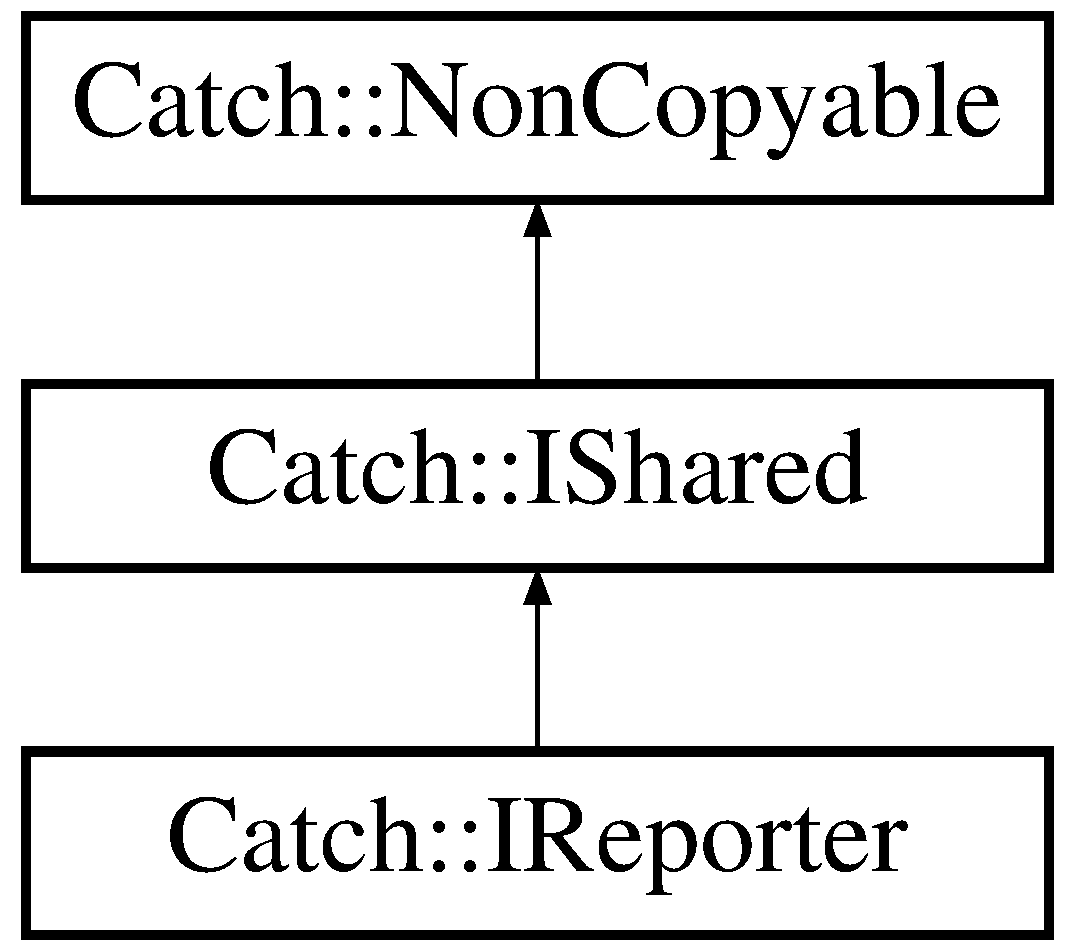
\includegraphics[height=3.000000cm]{classCatch_1_1NonCopyable}
\end{center}
\end{figure}
\subsubsection*{Protected Member Functions}
\begin{DoxyCompactItemize}
\item 
\hyperlink{classCatch_1_1NonCopyable_a4b492dd5753f9952350fb64dc6cb9fe2}{Non\-Copyable} ()
\item 
virtual \hyperlink{classCatch_1_1NonCopyable_a81254677280fef337eb4a676e91e3293}{$\sim$\-Non\-Copyable} ()
\end{DoxyCompactItemize}


\subsubsection{Constructor \& Destructor Documentation}
\hypertarget{classCatch_1_1NonCopyable_a4b492dd5753f9952350fb64dc6cb9fe2}{\index{Catch\-::\-Non\-Copyable@{Catch\-::\-Non\-Copyable}!Non\-Copyable@{Non\-Copyable}}
\index{Non\-Copyable@{Non\-Copyable}!Catch::NonCopyable@{Catch\-::\-Non\-Copyable}}
\paragraph[{Non\-Copyable}]{\setlength{\rightskip}{0pt plus 5cm}Catch\-::\-Non\-Copyable\-::\-Non\-Copyable (
\begin{DoxyParamCaption}
{}
\end{DoxyParamCaption}
)\hspace{0.3cm}{\ttfamily [inline]}, {\ttfamily [protected]}}}\label{classCatch_1_1NonCopyable_a4b492dd5753f9952350fb64dc6cb9fe2}
\hypertarget{classCatch_1_1NonCopyable_a81254677280fef337eb4a676e91e3293}{\index{Catch\-::\-Non\-Copyable@{Catch\-::\-Non\-Copyable}!$\sim$\-Non\-Copyable@{$\sim$\-Non\-Copyable}}
\index{$\sim$\-Non\-Copyable@{$\sim$\-Non\-Copyable}!Catch::NonCopyable@{Catch\-::\-Non\-Copyable}}
\paragraph[{$\sim$\-Non\-Copyable}]{\setlength{\rightskip}{0pt plus 5cm}virtual Catch\-::\-Non\-Copyable\-::$\sim$\-Non\-Copyable (
\begin{DoxyParamCaption}
{}
\end{DoxyParamCaption}
)\hspace{0.3cm}{\ttfamily [inline]}, {\ttfamily [protected]}, {\ttfamily [virtual]}}}\label{classCatch_1_1NonCopyable_a81254677280fef337eb4a676e91e3293}


The documentation for this class was generated from the following file\-:\begin{DoxyCompactItemize}
\item 
include/\hyperlink{catch_8hpp}{catch.\-hpp}\end{DoxyCompactItemize}

\hypertarget{structCatch_1_1Detail_1_1NonStreamable}{\subsection{Catch\-:\-:Detail\-:\-:Non\-Streamable Struct Reference}
\label{structCatch_1_1Detail_1_1NonStreamable}\index{Catch\-::\-Detail\-::\-Non\-Streamable@{Catch\-::\-Detail\-::\-Non\-Streamable}}
}


{\ttfamily \#include $<$catch.\-hpp$>$}

\subsubsection*{Public Member Functions}
\begin{DoxyCompactItemize}
\item 
{\footnotesize template$<$typename T $>$ }\\\hyperlink{structCatch_1_1Detail_1_1NonStreamable_a891e9973c854291145e833bf8ed8d4de}{Non\-Streamable} (const T \&)
\end{DoxyCompactItemize}


\subsubsection{Constructor \& Destructor Documentation}
\hypertarget{structCatch_1_1Detail_1_1NonStreamable_a891e9973c854291145e833bf8ed8d4de}{\index{Catch\-::\-Detail\-::\-Non\-Streamable@{Catch\-::\-Detail\-::\-Non\-Streamable}!Non\-Streamable@{Non\-Streamable}}
\index{Non\-Streamable@{Non\-Streamable}!Catch::Detail::NonStreamable@{Catch\-::\-Detail\-::\-Non\-Streamable}}
\paragraph[{Non\-Streamable}]{\setlength{\rightskip}{0pt plus 5cm}template$<$typename T $>$ Catch\-::\-Detail\-::\-Non\-Streamable\-::\-Non\-Streamable (
\begin{DoxyParamCaption}
\item[{const T \&}]{}
\end{DoxyParamCaption}
)\hspace{0.3cm}{\ttfamily [inline]}}}\label{structCatch_1_1Detail_1_1NonStreamable_a891e9973c854291145e833bf8ed8d4de}


The documentation for this struct was generated from the following file\-:\begin{DoxyCompactItemize}
\item 
include/\hyperlink{catch_8hpp}{catch.\-hpp}\end{DoxyCompactItemize}

\hypertarget{classprediction_1_1NormalAdaptationPredictionParameters}{\subsection{prediction.\-Normal\-Adaptation\-Prediction\-Parameters Class Reference}
\label{classprediction_1_1NormalAdaptationPredictionParameters}\index{prediction.\-Normal\-Adaptation\-Prediction\-Parameters@{prediction.\-Normal\-Adaptation\-Prediction\-Parameters}}
}
Inheritance diagram for prediction.\-Normal\-Adaptation\-Prediction\-Parameters\-:\begin{figure}[H]
\begin{center}
\leavevmode
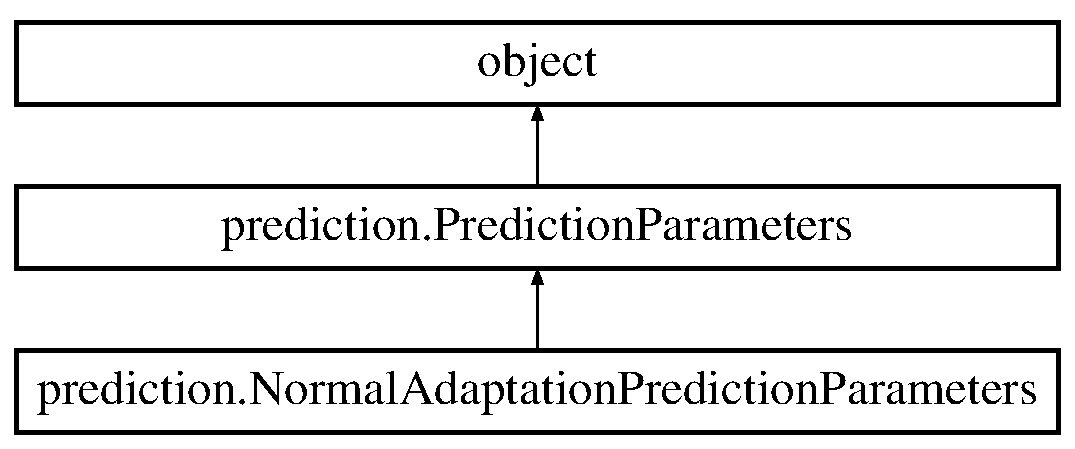
\includegraphics[height=3.000000cm]{classprediction_1_1NormalAdaptationPredictionParameters}
\end{center}
\end{figure}
\subsubsection*{Public Member Functions}
\begin{DoxyCompactItemize}
\item 
def \hyperlink{classprediction_1_1NormalAdaptationPredictionParameters_a37a683e612fdd25761db1251dff0312e}{\-\_\-\-\_\-init\-\_\-\-\_\-}
\item 
def \hyperlink{classprediction_1_1NormalAdaptationPredictionParameters_a271e277b0443ecc8eb207be582ddf057}{\-\_\-\-\_\-str\-\_\-\-\_\-}
\item 
def \hyperlink{classprediction_1_1NormalAdaptationPredictionParameters_acf7a3750f91f8c6fee0b2b384a5ca402}{generate\-Predicted\-Trajectories}
\end{DoxyCompactItemize}
\subsubsection*{Public Attributes}
\begin{DoxyCompactItemize}
\item 
\hyperlink{classprediction_1_1NormalAdaptationPredictionParameters_a34b3cdb524d0014193976f43ff8c7117}{n\-Predicted\-Trajectories}
\item 
\hyperlink{classprediction_1_1NormalAdaptationPredictionParameters_aa8f623907e9b858e119f5675f988e5ea}{use\-Features}
\item 
\hyperlink{classprediction_1_1NormalAdaptationPredictionParameters_a816e2961bc7aeb7637228d994a5f62d9}{acceleration\-Distribution}
\item 
\hyperlink{classprediction_1_1NormalAdaptationPredictionParameters_a27699c7d260535dd7a656cdc6d00d94e}{steering\-Distribution}
\end{DoxyCompactItemize}


\subsubsection{Constructor \& Destructor Documentation}
\hypertarget{classprediction_1_1NormalAdaptationPredictionParameters_a37a683e612fdd25761db1251dff0312e}{\index{prediction\-::\-Normal\-Adaptation\-Prediction\-Parameters@{prediction\-::\-Normal\-Adaptation\-Prediction\-Parameters}!\-\_\-\-\_\-init\-\_\-\-\_\-@{\-\_\-\-\_\-init\-\_\-\-\_\-}}
\index{\-\_\-\-\_\-init\-\_\-\-\_\-@{\-\_\-\-\_\-init\-\_\-\-\_\-}!prediction::NormalAdaptationPredictionParameters@{prediction\-::\-Normal\-Adaptation\-Prediction\-Parameters}}
\paragraph[{\-\_\-\-\_\-init\-\_\-\-\_\-}]{\setlength{\rightskip}{0pt plus 5cm}def prediction.\-Normal\-Adaptation\-Prediction\-Parameters.\-\_\-\-\_\-init\-\_\-\-\_\- (
\begin{DoxyParamCaption}
\item[{}]{self, }
\item[{}]{max\-Speed, }
\item[{}]{n\-Predicted\-Trajectories, }
\item[{}]{acceleration\-Distribution, }
\item[{}]{steering\-Distribution, }
\item[{}]{use\-Features = {\ttfamily False}}
\end{DoxyParamCaption}
)}}\label{classprediction_1_1NormalAdaptationPredictionParameters_a37a683e612fdd25761db1251dff0312e}
\begin{DoxyVerb}An example of acceleration and steering distributions is
lambda: random.triangular(-self.maxAcceleration, self.maxAcceleration, 0.)
\end{DoxyVerb}
 

\subsubsection{Member Function Documentation}
\hypertarget{classprediction_1_1NormalAdaptationPredictionParameters_a271e277b0443ecc8eb207be582ddf057}{\index{prediction\-::\-Normal\-Adaptation\-Prediction\-Parameters@{prediction\-::\-Normal\-Adaptation\-Prediction\-Parameters}!\-\_\-\-\_\-str\-\_\-\-\_\-@{\-\_\-\-\_\-str\-\_\-\-\_\-}}
\index{\-\_\-\-\_\-str\-\_\-\-\_\-@{\-\_\-\-\_\-str\-\_\-\-\_\-}!prediction::NormalAdaptationPredictionParameters@{prediction\-::\-Normal\-Adaptation\-Prediction\-Parameters}}
\paragraph[{\-\_\-\-\_\-str\-\_\-\-\_\-}]{\setlength{\rightskip}{0pt plus 5cm}def prediction.\-Normal\-Adaptation\-Prediction\-Parameters.\-\_\-\-\_\-str\-\_\-\-\_\- (
\begin{DoxyParamCaption}
\item[{}]{self}
\end{DoxyParamCaption}
)}}\label{classprediction_1_1NormalAdaptationPredictionParameters_a271e277b0443ecc8eb207be582ddf057}


References K\-L\-T\-Feature\-Tracking\-Parameters.\-max\-Acceleration, K\-L\-T\-Feature\-Tracking\-Parameters.\-max\-Steering, K\-L\-T\-Feature\-Tracking\-Parameters.\-n\-Predicted\-Trajectories, and prediction.\-Normal\-Adaptation\-Prediction\-Parameters.\-n\-Predicted\-Trajectories.

\hypertarget{classprediction_1_1NormalAdaptationPredictionParameters_acf7a3750f91f8c6fee0b2b384a5ca402}{\index{prediction\-::\-Normal\-Adaptation\-Prediction\-Parameters@{prediction\-::\-Normal\-Adaptation\-Prediction\-Parameters}!generate\-Predicted\-Trajectories@{generate\-Predicted\-Trajectories}}
\index{generate\-Predicted\-Trajectories@{generate\-Predicted\-Trajectories}!prediction::NormalAdaptationPredictionParameters@{prediction\-::\-Normal\-Adaptation\-Prediction\-Parameters}}
\paragraph[{generate\-Predicted\-Trajectories}]{\setlength{\rightskip}{0pt plus 5cm}def prediction.\-Normal\-Adaptation\-Prediction\-Parameters.\-generate\-Predicted\-Trajectories (
\begin{DoxyParamCaption}
\item[{}]{self, }
\item[{}]{obj, }
\item[{}]{instant}
\end{DoxyParamCaption}
)}}\label{classprediction_1_1NormalAdaptationPredictionParameters_acf7a3750f91f8c6fee0b2b384a5ca402}


References prediction.\-Predicted\-Trajectory\-Random\-Control.\-acceleration\-Distribution, prediction.\-Normal\-Adaptation\-Prediction\-Parameters.\-acceleration\-Distribution, prediction.\-Predicted\-Trajectory\-Constant.\-max\-Speed, prediction.\-Predicted\-Trajectory\-Random\-Control.\-max\-Speed, prediction.\-Prediction\-Parameters.\-max\-Speed, K\-L\-T\-Feature\-Tracking\-Parameters.\-n\-Predicted\-Trajectories, prediction.\-Normal\-Adaptation\-Prediction\-Parameters.\-n\-Predicted\-Trajectories, prediction.\-Predicted\-Trajectory\-Random\-Control.\-steering\-Distribution, prediction.\-Normal\-Adaptation\-Prediction\-Parameters.\-steering\-Distribution, and prediction.\-Normal\-Adaptation\-Prediction\-Parameters.\-use\-Features.



\subsubsection{Member Data Documentation}
\hypertarget{classprediction_1_1NormalAdaptationPredictionParameters_a816e2961bc7aeb7637228d994a5f62d9}{\index{prediction\-::\-Normal\-Adaptation\-Prediction\-Parameters@{prediction\-::\-Normal\-Adaptation\-Prediction\-Parameters}!acceleration\-Distribution@{acceleration\-Distribution}}
\index{acceleration\-Distribution@{acceleration\-Distribution}!prediction::NormalAdaptationPredictionParameters@{prediction\-::\-Normal\-Adaptation\-Prediction\-Parameters}}
\paragraph[{acceleration\-Distribution}]{\setlength{\rightskip}{0pt plus 5cm}prediction.\-Normal\-Adaptation\-Prediction\-Parameters.\-acceleration\-Distribution}}\label{classprediction_1_1NormalAdaptationPredictionParameters_a816e2961bc7aeb7637228d994a5f62d9}
\hypertarget{classprediction_1_1NormalAdaptationPredictionParameters_a34b3cdb524d0014193976f43ff8c7117}{\index{prediction\-::\-Normal\-Adaptation\-Prediction\-Parameters@{prediction\-::\-Normal\-Adaptation\-Prediction\-Parameters}!n\-Predicted\-Trajectories@{n\-Predicted\-Trajectories}}
\index{n\-Predicted\-Trajectories@{n\-Predicted\-Trajectories}!prediction::NormalAdaptationPredictionParameters@{prediction\-::\-Normal\-Adaptation\-Prediction\-Parameters}}
\paragraph[{n\-Predicted\-Trajectories}]{\setlength{\rightskip}{0pt plus 5cm}prediction.\-Normal\-Adaptation\-Prediction\-Parameters.\-n\-Predicted\-Trajectories}}\label{classprediction_1_1NormalAdaptationPredictionParameters_a34b3cdb524d0014193976f43ff8c7117}
\hypertarget{classprediction_1_1NormalAdaptationPredictionParameters_a27699c7d260535dd7a656cdc6d00d94e}{\index{prediction\-::\-Normal\-Adaptation\-Prediction\-Parameters@{prediction\-::\-Normal\-Adaptation\-Prediction\-Parameters}!steering\-Distribution@{steering\-Distribution}}
\index{steering\-Distribution@{steering\-Distribution}!prediction::NormalAdaptationPredictionParameters@{prediction\-::\-Normal\-Adaptation\-Prediction\-Parameters}}
\paragraph[{steering\-Distribution}]{\setlength{\rightskip}{0pt plus 5cm}prediction.\-Normal\-Adaptation\-Prediction\-Parameters.\-steering\-Distribution}}\label{classprediction_1_1NormalAdaptationPredictionParameters_a27699c7d260535dd7a656cdc6d00d94e}
\hypertarget{classprediction_1_1NormalAdaptationPredictionParameters_aa8f623907e9b858e119f5675f988e5ea}{\index{prediction\-::\-Normal\-Adaptation\-Prediction\-Parameters@{prediction\-::\-Normal\-Adaptation\-Prediction\-Parameters}!use\-Features@{use\-Features}}
\index{use\-Features@{use\-Features}!prediction::NormalAdaptationPredictionParameters@{prediction\-::\-Normal\-Adaptation\-Prediction\-Parameters}}
\paragraph[{use\-Features}]{\setlength{\rightskip}{0pt plus 5cm}prediction.\-Normal\-Adaptation\-Prediction\-Parameters.\-use\-Features}}\label{classprediction_1_1NormalAdaptationPredictionParameters_aa8f623907e9b858e119f5675f988e5ea}


The documentation for this class was generated from the following file\-:\begin{DoxyCompactItemize}
\item 
python/\hyperlink{prediction_8py}{prediction.\-py}\end{DoxyCompactItemize}

\hypertarget{classmoving_1_1NormAngle}{\subsection{moving.\-Norm\-Angle Class Reference}
\label{classmoving_1_1NormAngle}\index{moving.\-Norm\-Angle@{moving.\-Norm\-Angle}}
}
Inheritance diagram for moving.\-Norm\-Angle\-:\begin{figure}[H]
\begin{center}
\leavevmode
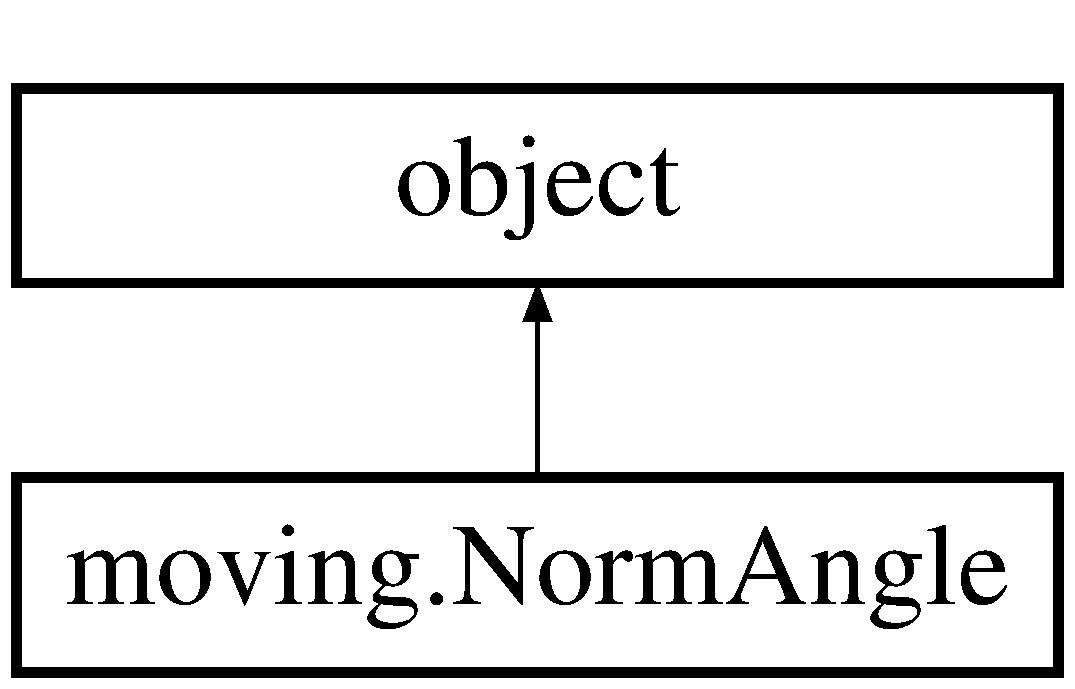
\includegraphics[height=2.000000cm]{classmoving_1_1NormAngle}
\end{center}
\end{figure}
\subsubsection*{Public Member Functions}
\begin{DoxyCompactItemize}
\item 
def \hyperlink{classmoving_1_1NormAngle_a12d558d559a2dfd98725ba14e88678f8}{\-\_\-\-\_\-init\-\_\-\-\_\-}
\item 
def \hyperlink{classmoving_1_1NormAngle_ae02427390608a55ed603a45f530713cf}{\-\_\-\-\_\-add\-\_\-\-\_\-}
\item 
def \hyperlink{classmoving_1_1NormAngle_a974791421e05b5df0a1a7b7932561a4e}{get\-Point}
\end{DoxyCompactItemize}
\subsubsection*{Static Public Member Functions}
\begin{DoxyCompactItemize}
\item 
def \hyperlink{classmoving_1_1NormAngle_a32cec3b7beb598f4c41c8f540b636b75}{from\-Point}
\end{DoxyCompactItemize}
\subsubsection*{Public Attributes}
\begin{DoxyCompactItemize}
\item 
\hyperlink{classmoving_1_1NormAngle_aa1c83abb2f11a937badd1bb77efc5c87}{norm}
\item 
\hyperlink{classmoving_1_1NormAngle_a1849471fc66f5facf2380870819359f5}{angle}
\end{DoxyCompactItemize}


\subsubsection{Detailed Description}
\begin{DoxyVerb}Alternate encoding of a point, by its norm and orientation\end{DoxyVerb}
 

\subsubsection{Constructor \& Destructor Documentation}
\hypertarget{classmoving_1_1NormAngle_a12d558d559a2dfd98725ba14e88678f8}{\index{moving\-::\-Norm\-Angle@{moving\-::\-Norm\-Angle}!\-\_\-\-\_\-init\-\_\-\-\_\-@{\-\_\-\-\_\-init\-\_\-\-\_\-}}
\index{\-\_\-\-\_\-init\-\_\-\-\_\-@{\-\_\-\-\_\-init\-\_\-\-\_\-}!moving::NormAngle@{moving\-::\-Norm\-Angle}}
\paragraph[{\-\_\-\-\_\-init\-\_\-\-\_\-}]{\setlength{\rightskip}{0pt plus 5cm}def moving.\-Norm\-Angle.\-\_\-\-\_\-init\-\_\-\-\_\- (
\begin{DoxyParamCaption}
\item[{}]{self, }
\item[{}]{norm, }
\item[{}]{angle}
\end{DoxyParamCaption}
)}}\label{classmoving_1_1NormAngle_a12d558d559a2dfd98725ba14e88678f8}


\subsubsection{Member Function Documentation}
\hypertarget{classmoving_1_1NormAngle_ae02427390608a55ed603a45f530713cf}{\index{moving\-::\-Norm\-Angle@{moving\-::\-Norm\-Angle}!\-\_\-\-\_\-add\-\_\-\-\_\-@{\-\_\-\-\_\-add\-\_\-\-\_\-}}
\index{\-\_\-\-\_\-add\-\_\-\-\_\-@{\-\_\-\-\_\-add\-\_\-\-\_\-}!moving::NormAngle@{moving\-::\-Norm\-Angle}}
\paragraph[{\-\_\-\-\_\-add\-\_\-\-\_\-}]{\setlength{\rightskip}{0pt plus 5cm}def moving.\-Norm\-Angle.\-\_\-\-\_\-add\-\_\-\-\_\- (
\begin{DoxyParamCaption}
\item[{}]{self, }
\item[{}]{other}
\end{DoxyParamCaption}
)}}\label{classmoving_1_1NormAngle_ae02427390608a55ed603a45f530713cf}


References moving.\-Norm\-Angle.\-angle, and moving.\-Norm\-Angle.\-norm.

\hypertarget{classmoving_1_1NormAngle_a32cec3b7beb598f4c41c8f540b636b75}{\index{moving\-::\-Norm\-Angle@{moving\-::\-Norm\-Angle}!from\-Point@{from\-Point}}
\index{from\-Point@{from\-Point}!moving::NormAngle@{moving\-::\-Norm\-Angle}}
\paragraph[{from\-Point}]{\setlength{\rightskip}{0pt plus 5cm}def moving.\-Norm\-Angle.\-from\-Point (
\begin{DoxyParamCaption}
\item[{}]{p}
\end{DoxyParamCaption}
)\hspace{0.3cm}{\ttfamily [static]}}}\label{classmoving_1_1NormAngle_a32cec3b7beb598f4c41c8f540b636b75}
\hypertarget{classmoving_1_1NormAngle_a974791421e05b5df0a1a7b7932561a4e}{\index{moving\-::\-Norm\-Angle@{moving\-::\-Norm\-Angle}!get\-Point@{get\-Point}}
\index{get\-Point@{get\-Point}!moving::NormAngle@{moving\-::\-Norm\-Angle}}
\paragraph[{get\-Point}]{\setlength{\rightskip}{0pt plus 5cm}def moving.\-Norm\-Angle.\-get\-Point (
\begin{DoxyParamCaption}
\item[{}]{self}
\end{DoxyParamCaption}
)}}\label{classmoving_1_1NormAngle_a974791421e05b5df0a1a7b7932561a4e}


References moving.\-Norm\-Angle.\-angle, and moving.\-Norm\-Angle.\-norm.



\subsubsection{Member Data Documentation}
\hypertarget{classmoving_1_1NormAngle_a1849471fc66f5facf2380870819359f5}{\index{moving\-::\-Norm\-Angle@{moving\-::\-Norm\-Angle}!angle@{angle}}
\index{angle@{angle}!moving::NormAngle@{moving\-::\-Norm\-Angle}}
\paragraph[{angle}]{\setlength{\rightskip}{0pt plus 5cm}moving.\-Norm\-Angle.\-angle}}\label{classmoving_1_1NormAngle_a1849471fc66f5facf2380870819359f5}
\hypertarget{classmoving_1_1NormAngle_aa1c83abb2f11a937badd1bb77efc5c87}{\index{moving\-::\-Norm\-Angle@{moving\-::\-Norm\-Angle}!norm@{norm}}
\index{norm@{norm}!moving::NormAngle@{moving\-::\-Norm\-Angle}}
\paragraph[{norm}]{\setlength{\rightskip}{0pt plus 5cm}moving.\-Norm\-Angle.\-norm}}\label{classmoving_1_1NormAngle_aa1c83abb2f11a937badd1bb77efc5c87}


The documentation for this class was generated from the following file\-:\begin{DoxyCompactItemize}
\item 
python/\hyperlink{moving_8py}{moving.\-py}\end{DoxyCompactItemize}

\hypertarget{structCatch_1_1Internal_1_1OperatorTraits}{\subsection{Catch\-:\-:Internal\-:\-:Operator\-Traits$<$ Op $>$ Struct Template Reference}
\label{structCatch_1_1Internal_1_1OperatorTraits}\index{Catch\-::\-Internal\-::\-Operator\-Traits$<$ Op $>$@{Catch\-::\-Internal\-::\-Operator\-Traits$<$ Op $>$}}
}


{\ttfamily \#include $<$catch.\-hpp$>$}

\subsubsection*{Static Public Member Functions}
\begin{DoxyCompactItemize}
\item 
static const char $\ast$ \hyperlink{structCatch_1_1Internal_1_1OperatorTraits_ac6d08082ea33348d42bc4ccbd6d07671}{get\-Name} ()
\end{DoxyCompactItemize}


\subsubsection{Member Function Documentation}
\hypertarget{structCatch_1_1Internal_1_1OperatorTraits_ac6d08082ea33348d42bc4ccbd6d07671}{\index{Catch\-::\-Internal\-::\-Operator\-Traits@{Catch\-::\-Internal\-::\-Operator\-Traits}!get\-Name@{get\-Name}}
\index{get\-Name@{get\-Name}!Catch::Internal::OperatorTraits@{Catch\-::\-Internal\-::\-Operator\-Traits}}
\paragraph[{get\-Name}]{\setlength{\rightskip}{0pt plus 5cm}template$<$Operator Op$>$ static const char$\ast$ {\bf Catch\-::\-Internal\-::\-Operator\-Traits}$<$ Op $>$\-::get\-Name (
\begin{DoxyParamCaption}
{}
\end{DoxyParamCaption}
)\hspace{0.3cm}{\ttfamily [inline]}, {\ttfamily [static]}}}\label{structCatch_1_1Internal_1_1OperatorTraits_ac6d08082ea33348d42bc4ccbd6d07671}


References Catch\-::\-Internal\-::\-Operator\-Traits$<$ Op $>$\-::get\-Name().



The documentation for this struct was generated from the following file\-:\begin{DoxyCompactItemize}
\item 
include/\hyperlink{catch_8hpp}{catch.\-hpp}\end{DoxyCompactItemize}

\hypertarget{structCatch_1_1Internal_1_1OperatorTraits_3_01IsEqualTo_01_4}{\subsection{Catch\-:\-:Internal\-:\-:Operator\-Traits$<$ Is\-Equal\-To $>$ Struct Template Reference}
\label{structCatch_1_1Internal_1_1OperatorTraits_3_01IsEqualTo_01_4}\index{Catch\-::\-Internal\-::\-Operator\-Traits$<$ Is\-Equal\-To $>$@{Catch\-::\-Internal\-::\-Operator\-Traits$<$ Is\-Equal\-To $>$}}
}


{\ttfamily \#include $<$catch.\-hpp$>$}

\subsubsection*{Static Public Member Functions}
\begin{DoxyCompactItemize}
\item 
static const char $\ast$ \hyperlink{structCatch_1_1Internal_1_1OperatorTraits_3_01IsEqualTo_01_4_addf03ac66f0ed83abcc037a7a327d4f1}{get\-Name} ()
\end{DoxyCompactItemize}


\subsubsection{Member Function Documentation}
\hypertarget{structCatch_1_1Internal_1_1OperatorTraits_3_01IsEqualTo_01_4_addf03ac66f0ed83abcc037a7a327d4f1}{\index{Catch\-::\-Internal\-::\-Operator\-Traits$<$ Is\-Equal\-To $>$@{Catch\-::\-Internal\-::\-Operator\-Traits$<$ Is\-Equal\-To $>$}!get\-Name@{get\-Name}}
\index{get\-Name@{get\-Name}!Catch::Internal::OperatorTraits< IsEqualTo >@{Catch\-::\-Internal\-::\-Operator\-Traits$<$ Is\-Equal\-To $>$}}
\paragraph[{get\-Name}]{\setlength{\rightskip}{0pt plus 5cm}static const char$\ast$ {\bf Catch\-::\-Internal\-::\-Operator\-Traits}$<$ {\bf Is\-Equal\-To} $>$\-::get\-Name (
\begin{DoxyParamCaption}
{}
\end{DoxyParamCaption}
)\hspace{0.3cm}{\ttfamily [inline]}, {\ttfamily [static]}}}\label{structCatch_1_1Internal_1_1OperatorTraits_3_01IsEqualTo_01_4_addf03ac66f0ed83abcc037a7a327d4f1}


References get\-Name().



The documentation for this struct was generated from the following file\-:\begin{DoxyCompactItemize}
\item 
include/\hyperlink{catch_8hpp}{catch.\-hpp}\end{DoxyCompactItemize}

\hypertarget{structCatch_1_1Internal_1_1OperatorTraits_3_01IsGreaterThan_01_4}{\subsection{Catch\-:\-:Internal\-:\-:Operator\-Traits$<$ Is\-Greater\-Than $>$ Struct Template Reference}
\label{structCatch_1_1Internal_1_1OperatorTraits_3_01IsGreaterThan_01_4}\index{Catch\-::\-Internal\-::\-Operator\-Traits$<$ Is\-Greater\-Than $>$@{Catch\-::\-Internal\-::\-Operator\-Traits$<$ Is\-Greater\-Than $>$}}
}


{\ttfamily \#include $<$catch.\-hpp$>$}

\subsubsection*{Static Public Member Functions}
\begin{DoxyCompactItemize}
\item 
static const char $\ast$ \hyperlink{structCatch_1_1Internal_1_1OperatorTraits_3_01IsGreaterThan_01_4_ab917bfb9ccbe461dc684ee5a34d67d27}{get\-Name} ()
\end{DoxyCompactItemize}


\subsubsection{Member Function Documentation}
\hypertarget{structCatch_1_1Internal_1_1OperatorTraits_3_01IsGreaterThan_01_4_ab917bfb9ccbe461dc684ee5a34d67d27}{\index{Catch\-::\-Internal\-::\-Operator\-Traits$<$ Is\-Greater\-Than $>$@{Catch\-::\-Internal\-::\-Operator\-Traits$<$ Is\-Greater\-Than $>$}!get\-Name@{get\-Name}}
\index{get\-Name@{get\-Name}!Catch::Internal::OperatorTraits< IsGreaterThan >@{Catch\-::\-Internal\-::\-Operator\-Traits$<$ Is\-Greater\-Than $>$}}
\paragraph[{get\-Name}]{\setlength{\rightskip}{0pt plus 5cm}static const char$\ast$ {\bf Catch\-::\-Internal\-::\-Operator\-Traits}$<$ {\bf Is\-Greater\-Than} $>$\-::get\-Name (
\begin{DoxyParamCaption}
{}
\end{DoxyParamCaption}
)\hspace{0.3cm}{\ttfamily [inline]}, {\ttfamily [static]}}}\label{structCatch_1_1Internal_1_1OperatorTraits_3_01IsGreaterThan_01_4_ab917bfb9ccbe461dc684ee5a34d67d27}


References get\-Name().



The documentation for this struct was generated from the following file\-:\begin{DoxyCompactItemize}
\item 
include/\hyperlink{catch_8hpp}{catch.\-hpp}\end{DoxyCompactItemize}

\hypertarget{structCatch_1_1Internal_1_1OperatorTraits_3_01IsGreaterThanOrEqualTo_01_4}{\subsection{Catch\-:\-:Internal\-:\-:Operator\-Traits$<$ Is\-Greater\-Than\-Or\-Equal\-To $>$ Struct Template Reference}
\label{structCatch_1_1Internal_1_1OperatorTraits_3_01IsGreaterThanOrEqualTo_01_4}\index{Catch\-::\-Internal\-::\-Operator\-Traits$<$ Is\-Greater\-Than\-Or\-Equal\-To $>$@{Catch\-::\-Internal\-::\-Operator\-Traits$<$ Is\-Greater\-Than\-Or\-Equal\-To $>$}}
}


{\ttfamily \#include $<$catch.\-hpp$>$}

\subsubsection*{Static Public Member Functions}
\begin{DoxyCompactItemize}
\item 
static const char $\ast$ \hyperlink{structCatch_1_1Internal_1_1OperatorTraits_3_01IsGreaterThanOrEqualTo_01_4_a76b6f6b0dbaf7d19ebb1b4b4891e719e}{get\-Name} ()
\end{DoxyCompactItemize}


\subsubsection{Member Function Documentation}
\hypertarget{structCatch_1_1Internal_1_1OperatorTraits_3_01IsGreaterThanOrEqualTo_01_4_a76b6f6b0dbaf7d19ebb1b4b4891e719e}{\index{Catch\-::\-Internal\-::\-Operator\-Traits$<$ Is\-Greater\-Than\-Or\-Equal\-To $>$@{Catch\-::\-Internal\-::\-Operator\-Traits$<$ Is\-Greater\-Than\-Or\-Equal\-To $>$}!get\-Name@{get\-Name}}
\index{get\-Name@{get\-Name}!Catch::Internal::OperatorTraits< IsGreaterThanOrEqualTo >@{Catch\-::\-Internal\-::\-Operator\-Traits$<$ Is\-Greater\-Than\-Or\-Equal\-To $>$}}
\paragraph[{get\-Name}]{\setlength{\rightskip}{0pt plus 5cm}static const char$\ast$ {\bf Catch\-::\-Internal\-::\-Operator\-Traits}$<$ {\bf Is\-Greater\-Than\-Or\-Equal\-To} $>$\-::get\-Name (
\begin{DoxyParamCaption}
{}
\end{DoxyParamCaption}
)\hspace{0.3cm}{\ttfamily [inline]}, {\ttfamily [static]}}}\label{structCatch_1_1Internal_1_1OperatorTraits_3_01IsGreaterThanOrEqualTo_01_4_a76b6f6b0dbaf7d19ebb1b4b4891e719e}


References get\-Name().



The documentation for this struct was generated from the following file\-:\begin{DoxyCompactItemize}
\item 
include/\hyperlink{catch_8hpp}{catch.\-hpp}\end{DoxyCompactItemize}

\hypertarget{structCatch_1_1Internal_1_1OperatorTraits_3_01IsLessThan_01_4}{\subsection{Catch\-:\-:Internal\-:\-:Operator\-Traits$<$ Is\-Less\-Than $>$ Struct Template Reference}
\label{structCatch_1_1Internal_1_1OperatorTraits_3_01IsLessThan_01_4}\index{Catch\-::\-Internal\-::\-Operator\-Traits$<$ Is\-Less\-Than $>$@{Catch\-::\-Internal\-::\-Operator\-Traits$<$ Is\-Less\-Than $>$}}
}


{\ttfamily \#include $<$catch.\-hpp$>$}

\subsubsection*{Static Public Member Functions}
\begin{DoxyCompactItemize}
\item 
static const char $\ast$ \hyperlink{structCatch_1_1Internal_1_1OperatorTraits_3_01IsLessThan_01_4_aa3b536ddbd2e34b1253931ff00c32712}{get\-Name} ()
\end{DoxyCompactItemize}


\subsubsection{Member Function Documentation}
\hypertarget{structCatch_1_1Internal_1_1OperatorTraits_3_01IsLessThan_01_4_aa3b536ddbd2e34b1253931ff00c32712}{\index{Catch\-::\-Internal\-::\-Operator\-Traits$<$ Is\-Less\-Than $>$@{Catch\-::\-Internal\-::\-Operator\-Traits$<$ Is\-Less\-Than $>$}!get\-Name@{get\-Name}}
\index{get\-Name@{get\-Name}!Catch::Internal::OperatorTraits< IsLessThan >@{Catch\-::\-Internal\-::\-Operator\-Traits$<$ Is\-Less\-Than $>$}}
\paragraph[{get\-Name}]{\setlength{\rightskip}{0pt plus 5cm}static const char$\ast$ {\bf Catch\-::\-Internal\-::\-Operator\-Traits}$<$ {\bf Is\-Less\-Than} $>$\-::get\-Name (
\begin{DoxyParamCaption}
{}
\end{DoxyParamCaption}
)\hspace{0.3cm}{\ttfamily [inline]}, {\ttfamily [static]}}}\label{structCatch_1_1Internal_1_1OperatorTraits_3_01IsLessThan_01_4_aa3b536ddbd2e34b1253931ff00c32712}


References get\-Name().



The documentation for this struct was generated from the following file\-:\begin{DoxyCompactItemize}
\item 
include/\hyperlink{catch_8hpp}{catch.\-hpp}\end{DoxyCompactItemize}

\hypertarget{structCatch_1_1Internal_1_1OperatorTraits_3_01IsLessThanOrEqualTo_01_4}{\subsection{Catch\-:\-:Internal\-:\-:Operator\-Traits$<$ Is\-Less\-Than\-Or\-Equal\-To $>$ Struct Template Reference}
\label{structCatch_1_1Internal_1_1OperatorTraits_3_01IsLessThanOrEqualTo_01_4}\index{Catch\-::\-Internal\-::\-Operator\-Traits$<$ Is\-Less\-Than\-Or\-Equal\-To $>$@{Catch\-::\-Internal\-::\-Operator\-Traits$<$ Is\-Less\-Than\-Or\-Equal\-To $>$}}
}


{\ttfamily \#include $<$catch.\-hpp$>$}

\subsubsection*{Static Public Member Functions}
\begin{DoxyCompactItemize}
\item 
static const char $\ast$ \hyperlink{structCatch_1_1Internal_1_1OperatorTraits_3_01IsLessThanOrEqualTo_01_4_ae8578813bc847838f10448c1541a9d7b}{get\-Name} ()
\end{DoxyCompactItemize}


\subsubsection{Member Function Documentation}
\hypertarget{structCatch_1_1Internal_1_1OperatorTraits_3_01IsLessThanOrEqualTo_01_4_ae8578813bc847838f10448c1541a9d7b}{\index{Catch\-::\-Internal\-::\-Operator\-Traits$<$ Is\-Less\-Than\-Or\-Equal\-To $>$@{Catch\-::\-Internal\-::\-Operator\-Traits$<$ Is\-Less\-Than\-Or\-Equal\-To $>$}!get\-Name@{get\-Name}}
\index{get\-Name@{get\-Name}!Catch::Internal::OperatorTraits< IsLessThanOrEqualTo >@{Catch\-::\-Internal\-::\-Operator\-Traits$<$ Is\-Less\-Than\-Or\-Equal\-To $>$}}
\paragraph[{get\-Name}]{\setlength{\rightskip}{0pt plus 5cm}static const char$\ast$ {\bf Catch\-::\-Internal\-::\-Operator\-Traits}$<$ {\bf Is\-Less\-Than\-Or\-Equal\-To} $>$\-::get\-Name (
\begin{DoxyParamCaption}
{}
\end{DoxyParamCaption}
)\hspace{0.3cm}{\ttfamily [inline]}, {\ttfamily [static]}}}\label{structCatch_1_1Internal_1_1OperatorTraits_3_01IsLessThanOrEqualTo_01_4_ae8578813bc847838f10448c1541a9d7b}


References get\-Name().



The documentation for this struct was generated from the following file\-:\begin{DoxyCompactItemize}
\item 
include/\hyperlink{catch_8hpp}{catch.\-hpp}\end{DoxyCompactItemize}

\hypertarget{structCatch_1_1Internal_1_1OperatorTraits_3_01IsNotEqualTo_01_4}{\subsection{Catch\-:\-:Internal\-:\-:Operator\-Traits$<$ Is\-Not\-Equal\-To $>$ Struct Template Reference}
\label{structCatch_1_1Internal_1_1OperatorTraits_3_01IsNotEqualTo_01_4}\index{Catch\-::\-Internal\-::\-Operator\-Traits$<$ Is\-Not\-Equal\-To $>$@{Catch\-::\-Internal\-::\-Operator\-Traits$<$ Is\-Not\-Equal\-To $>$}}
}


{\ttfamily \#include $<$catch.\-hpp$>$}

\subsubsection*{Static Public Member Functions}
\begin{DoxyCompactItemize}
\item 
static const char $\ast$ \hyperlink{structCatch_1_1Internal_1_1OperatorTraits_3_01IsNotEqualTo_01_4_a54a795b8bf7c80a9fdbc7b81f39133b4}{get\-Name} ()
\end{DoxyCompactItemize}


\subsubsection{Member Function Documentation}
\hypertarget{structCatch_1_1Internal_1_1OperatorTraits_3_01IsNotEqualTo_01_4_a54a795b8bf7c80a9fdbc7b81f39133b4}{\index{Catch\-::\-Internal\-::\-Operator\-Traits$<$ Is\-Not\-Equal\-To $>$@{Catch\-::\-Internal\-::\-Operator\-Traits$<$ Is\-Not\-Equal\-To $>$}!get\-Name@{get\-Name}}
\index{get\-Name@{get\-Name}!Catch::Internal::OperatorTraits< IsNotEqualTo >@{Catch\-::\-Internal\-::\-Operator\-Traits$<$ Is\-Not\-Equal\-To $>$}}
\paragraph[{get\-Name}]{\setlength{\rightskip}{0pt plus 5cm}static const char$\ast$ {\bf Catch\-::\-Internal\-::\-Operator\-Traits}$<$ {\bf Is\-Not\-Equal\-To} $>$\-::get\-Name (
\begin{DoxyParamCaption}
{}
\end{DoxyParamCaption}
)\hspace{0.3cm}{\ttfamily [inline]}, {\ttfamily [static]}}}\label{structCatch_1_1Internal_1_1OperatorTraits_3_01IsNotEqualTo_01_4_a54a795b8bf7c80a9fdbc7b81f39133b4}


References get\-Name().



The documentation for this struct was generated from the following file\-:\begin{DoxyCompactItemize}
\item 
include/\hyperlink{catch_8hpp}{catch.\-hpp}\end{DoxyCompactItemize}

\hypertarget{classtraffic__engineering_1_1PassengerVehicle}{\subsection{traffic\-\_\-engineering.\-Passenger\-Vehicle Class Reference}
\label{classtraffic__engineering_1_1PassengerVehicle}\index{traffic\-\_\-engineering.\-Passenger\-Vehicle@{traffic\-\_\-engineering.\-Passenger\-Vehicle}}
}
Inheritance diagram for traffic\-\_\-engineering.\-Passenger\-Vehicle\-:\begin{figure}[H]
\begin{center}
\leavevmode
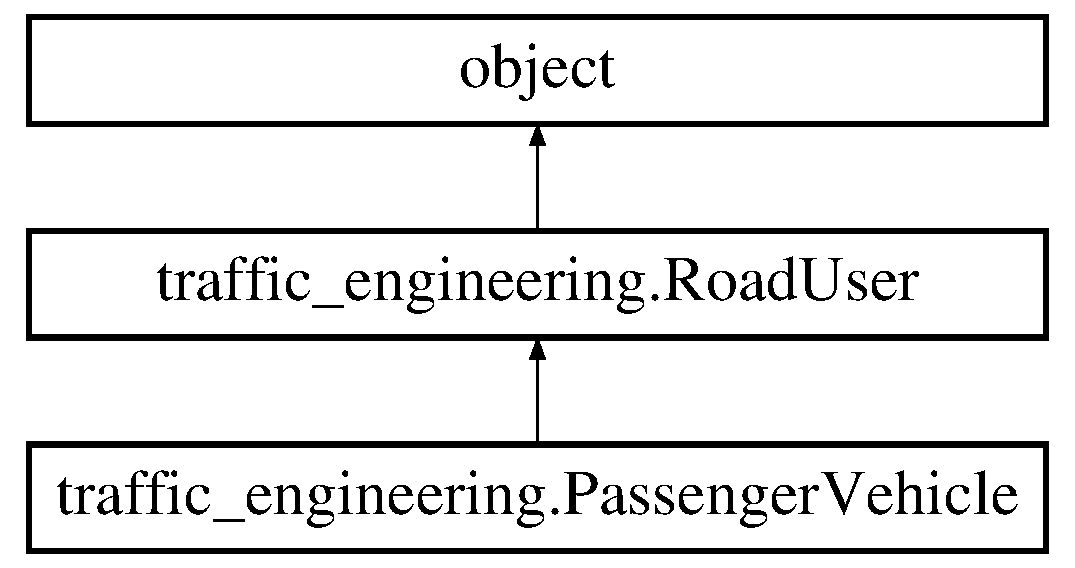
\includegraphics[height=3.000000cm]{classtraffic__engineering_1_1PassengerVehicle}
\end{center}
\end{figure}
\subsubsection*{Public Member Functions}
\begin{DoxyCompactItemize}
\item 
def \hyperlink{classtraffic__engineering_1_1PassengerVehicle_a33e9dc1b975771529dd45dd6d36ab5a6}{get\-Descriptor}
\end{DoxyCompactItemize}
\subsubsection*{Additional Inherited Members}


\subsubsection{Member Function Documentation}
\hypertarget{classtraffic__engineering_1_1PassengerVehicle_a33e9dc1b975771529dd45dd6d36ab5a6}{\index{traffic\-\_\-engineering\-::\-Passenger\-Vehicle@{traffic\-\_\-engineering\-::\-Passenger\-Vehicle}!get\-Descriptor@{get\-Descriptor}}
\index{get\-Descriptor@{get\-Descriptor}!traffic_engineering::PassengerVehicle@{traffic\-\_\-engineering\-::\-Passenger\-Vehicle}}
\paragraph[{get\-Descriptor}]{\setlength{\rightskip}{0pt plus 5cm}def traffic\-\_\-engineering.\-Passenger\-Vehicle.\-get\-Descriptor (
\begin{DoxyParamCaption}
\item[{}]{self}
\end{DoxyParamCaption}
)}}\label{classtraffic__engineering_1_1PassengerVehicle_a33e9dc1b975771529dd45dd6d36ab5a6}


The documentation for this class was generated from the following file\-:\begin{DoxyCompactItemize}
\item 
python/\hyperlink{traffic__engineering_8py}{traffic\-\_\-engineering.\-py}\end{DoxyCompactItemize}

\hypertarget{classtraffic__engineering_1_1Pedestrian}{\subsection{traffic\-\_\-engineering.\-Pedestrian Class Reference}
\label{classtraffic__engineering_1_1Pedestrian}\index{traffic\-\_\-engineering.\-Pedestrian@{traffic\-\_\-engineering.\-Pedestrian}}
}
Inheritance diagram for traffic\-\_\-engineering.\-Pedestrian\-:\begin{figure}[H]
\begin{center}
\leavevmode
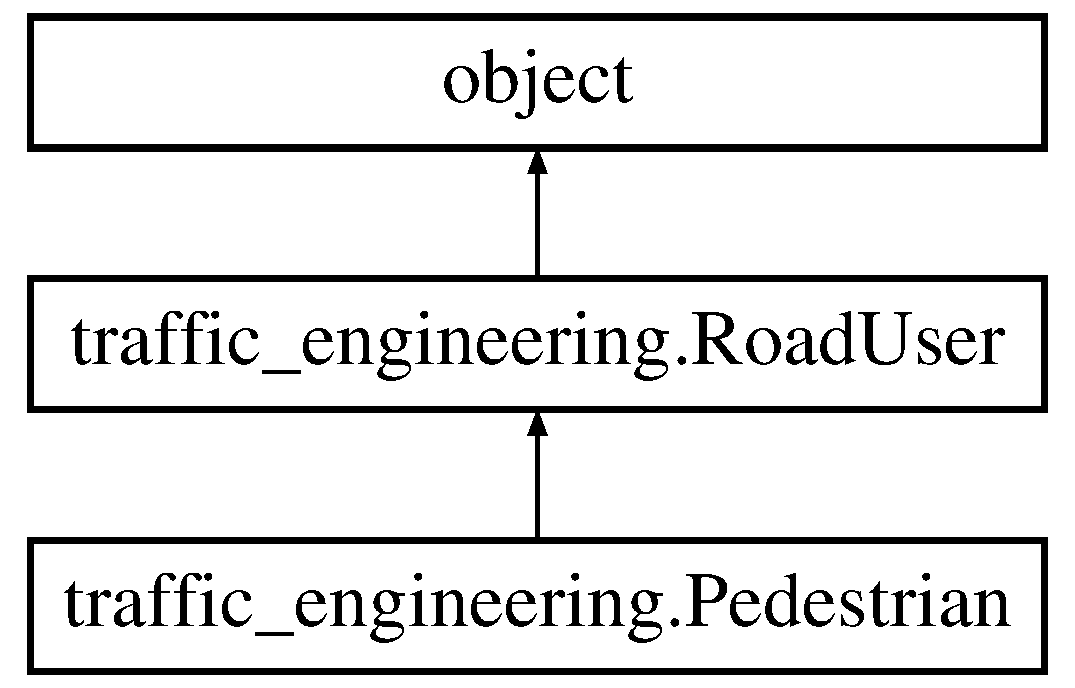
\includegraphics[height=3.000000cm]{classtraffic__engineering_1_1Pedestrian}
\end{center}
\end{figure}
\subsubsection*{Public Member Functions}
\begin{DoxyCompactItemize}
\item 
def \hyperlink{classtraffic__engineering_1_1Pedestrian_a9f3bbc5d7172d0b5fe74959e46c90192}{get\-Descriptor}
\end{DoxyCompactItemize}
\subsubsection*{Additional Inherited Members}


\subsubsection{Member Function Documentation}
\hypertarget{classtraffic__engineering_1_1Pedestrian_a9f3bbc5d7172d0b5fe74959e46c90192}{\index{traffic\-\_\-engineering\-::\-Pedestrian@{traffic\-\_\-engineering\-::\-Pedestrian}!get\-Descriptor@{get\-Descriptor}}
\index{get\-Descriptor@{get\-Descriptor}!traffic_engineering::Pedestrian@{traffic\-\_\-engineering\-::\-Pedestrian}}
\paragraph[{get\-Descriptor}]{\setlength{\rightskip}{0pt plus 5cm}def traffic\-\_\-engineering.\-Pedestrian.\-get\-Descriptor (
\begin{DoxyParamCaption}
\item[{}]{self}
\end{DoxyParamCaption}
)}}\label{classtraffic__engineering_1_1Pedestrian_a9f3bbc5d7172d0b5fe74959e46c90192}


The documentation for this class was generated from the following file\-:\begin{DoxyCompactItemize}
\item 
python/\hyperlink{traffic__engineering_8py}{traffic\-\_\-engineering.\-py}\end{DoxyCompactItemize}

\hypertarget{classmetadata_1_1Point}{\subsection{metadata.\-Point Class Reference}
\label{classmetadata_1_1Point}\index{metadata.\-Point@{metadata.\-Point}}
}
Inheritance diagram for metadata.\-Point\-:\begin{figure}[H]
\begin{center}
\leavevmode
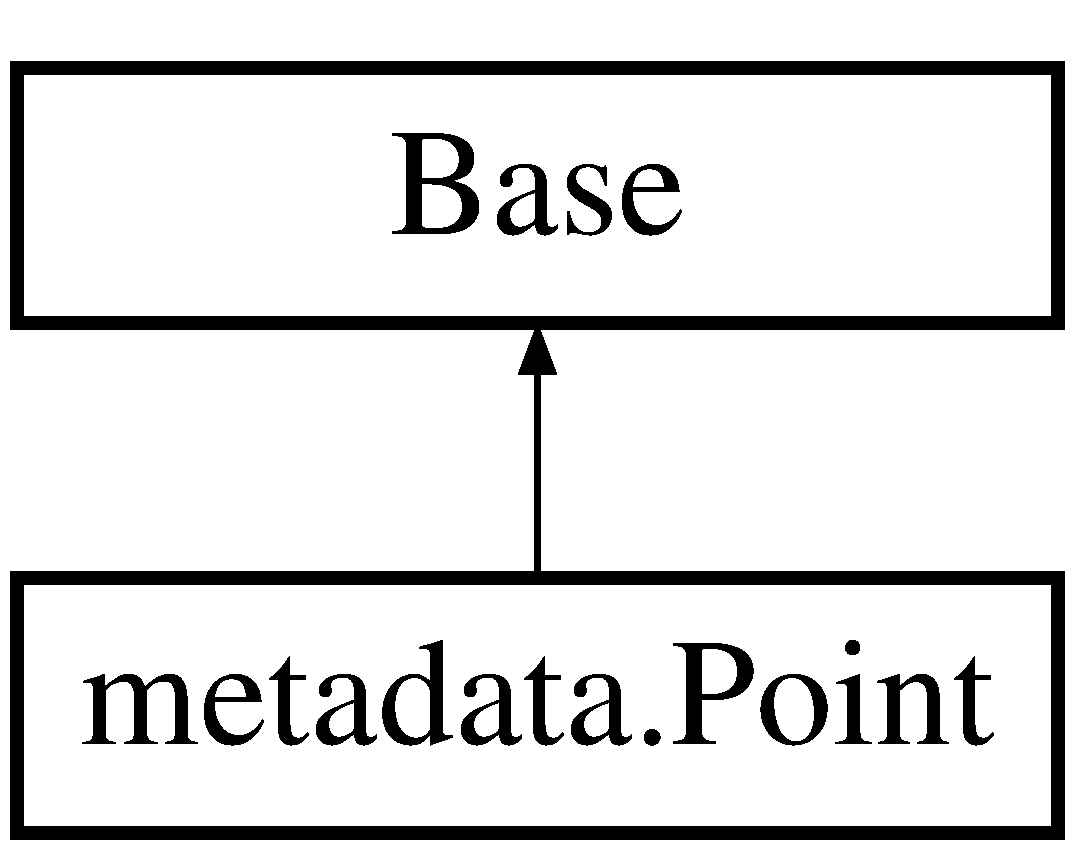
\includegraphics[height=2.000000cm]{classmetadata_1_1Point}
\end{center}
\end{figure}
\subsubsection*{Public Member Functions}
\begin{DoxyCompactItemize}
\item 
def \hyperlink{classmetadata_1_1Point_a81982cd2ff6f7ba831ce4745d88e5edd}{\-\_\-\-\_\-init\-\_\-\-\_\-}
\end{DoxyCompactItemize}
\subsubsection*{Public Attributes}
\begin{DoxyCompactItemize}
\item 
\hyperlink{classmetadata_1_1Point_ad295c4033b79c606357bb08faff0d8a2}{alignment\-Idx}
\item 
\hyperlink{classmetadata_1_1Point_a0d937f32b0ac686d9b38e3c186240443}{index}
\item 
\hyperlink{classmetadata_1_1Point_a6230a3f60e40936748114812a7395feb}{x}
\item 
\hyperlink{classmetadata_1_1Point_ab7539f5008fbb1bba9517dae88ef825d}{y}
\end{DoxyCompactItemize}
\subsubsection*{Static Public Attributes}
\begin{DoxyCompactItemize}
\item 
tuple \hyperlink{classmetadata_1_1Point_aca84ced91bcd73942f9b18b228eb067d}{alignment\-Idx} = Column(Integer, Foreign\-Key('alignments.\-idx'), primary\-\_\-key=True)
\item 
tuple \hyperlink{classmetadata_1_1Point_a705698f68fdde0a27f3fc9787c35e363}{index} = Column(Integer, primary\-\_\-key=True)
\item 
tuple \hyperlink{classmetadata_1_1Point_a7ef9864387912af9e0ff5fe4f19ac45e}{x} = Column(Float)
\item 
tuple \hyperlink{classmetadata_1_1Point_a88fd89923cd8eaa8104eb079eba80b85}{y} = Column(Float)
\item 
tuple \hyperlink{classmetadata_1_1Point_a3cbb7aebda686335a2f0cde52f0b24e2}{alignment} = relationship(\char`\"{}Alignment\char`\"{}, backref=backref('points', order\-\_\-by = \hyperlink{classmetadata_1_1Point_a705698f68fdde0a27f3fc9787c35e363}{index}))
\end{DoxyCompactItemize}


\subsubsection{Constructor \& Destructor Documentation}
\hypertarget{classmetadata_1_1Point_a81982cd2ff6f7ba831ce4745d88e5edd}{\index{metadata\-::\-Point@{metadata\-::\-Point}!\-\_\-\-\_\-init\-\_\-\-\_\-@{\-\_\-\-\_\-init\-\_\-\-\_\-}}
\index{\-\_\-\-\_\-init\-\_\-\-\_\-@{\-\_\-\-\_\-init\-\_\-\-\_\-}!metadata::Point@{metadata\-::\-Point}}
\paragraph[{\-\_\-\-\_\-init\-\_\-\-\_\-}]{\setlength{\rightskip}{0pt plus 5cm}def metadata.\-Point.\-\_\-\-\_\-init\-\_\-\-\_\- (
\begin{DoxyParamCaption}
\item[{}]{self, }
\item[{}]{alignment\-Idx, }
\item[{}]{index, }
\item[{}]{x, }
\item[{}]{y}
\end{DoxyParamCaption}
)}}\label{classmetadata_1_1Point_a81982cd2ff6f7ba831ce4745d88e5edd}


\subsubsection{Member Data Documentation}
\hypertarget{classmetadata_1_1Point_a3cbb7aebda686335a2f0cde52f0b24e2}{\index{metadata\-::\-Point@{metadata\-::\-Point}!alignment@{alignment}}
\index{alignment@{alignment}!metadata::Point@{metadata\-::\-Point}}
\paragraph[{alignment}]{\setlength{\rightskip}{0pt plus 5cm}tuple metadata.\-Point.\-alignment = relationship(\char`\"{}Alignment\char`\"{}, backref=backref('points', order\-\_\-by = {\bf index}))\hspace{0.3cm}{\ttfamily [static]}}}\label{classmetadata_1_1Point_a3cbb7aebda686335a2f0cde52f0b24e2}
\hypertarget{classmetadata_1_1Point_aca84ced91bcd73942f9b18b228eb067d}{\index{metadata\-::\-Point@{metadata\-::\-Point}!alignment\-Idx@{alignment\-Idx}}
\index{alignment\-Idx@{alignment\-Idx}!metadata::Point@{metadata\-::\-Point}}
\paragraph[{alignment\-Idx}]{\setlength{\rightskip}{0pt plus 5cm}tuple metadata.\-Point.\-alignment\-Idx = Column(Integer, Foreign\-Key('alignments.\-idx'), primary\-\_\-key=True)\hspace{0.3cm}{\ttfamily [static]}}}\label{classmetadata_1_1Point_aca84ced91bcd73942f9b18b228eb067d}
\hypertarget{classmetadata_1_1Point_ad295c4033b79c606357bb08faff0d8a2}{\index{metadata\-::\-Point@{metadata\-::\-Point}!alignment\-Idx@{alignment\-Idx}}
\index{alignment\-Idx@{alignment\-Idx}!metadata::Point@{metadata\-::\-Point}}
\paragraph[{alignment\-Idx}]{\setlength{\rightskip}{0pt plus 5cm}metadata.\-Point.\-alignment\-Idx}}\label{classmetadata_1_1Point_ad295c4033b79c606357bb08faff0d8a2}
\hypertarget{classmetadata_1_1Point_a705698f68fdde0a27f3fc9787c35e363}{\index{metadata\-::\-Point@{metadata\-::\-Point}!index@{index}}
\index{index@{index}!metadata::Point@{metadata\-::\-Point}}
\paragraph[{index}]{\setlength{\rightskip}{0pt plus 5cm}tuple metadata.\-Point.\-index = Column(Integer, primary\-\_\-key=True)\hspace{0.3cm}{\ttfamily [static]}}}\label{classmetadata_1_1Point_a705698f68fdde0a27f3fc9787c35e363}
\hypertarget{classmetadata_1_1Point_a0d937f32b0ac686d9b38e3c186240443}{\index{metadata\-::\-Point@{metadata\-::\-Point}!index@{index}}
\index{index@{index}!metadata::Point@{metadata\-::\-Point}}
\paragraph[{index}]{\setlength{\rightskip}{0pt plus 5cm}metadata.\-Point.\-index}}\label{classmetadata_1_1Point_a0d937f32b0ac686d9b38e3c186240443}
\hypertarget{classmetadata_1_1Point_a7ef9864387912af9e0ff5fe4f19ac45e}{\index{metadata\-::\-Point@{metadata\-::\-Point}!x@{x}}
\index{x@{x}!metadata::Point@{metadata\-::\-Point}}
\paragraph[{x}]{\setlength{\rightskip}{0pt plus 5cm}tuple metadata.\-Point.\-x = Column(Float)\hspace{0.3cm}{\ttfamily [static]}}}\label{classmetadata_1_1Point_a7ef9864387912af9e0ff5fe4f19ac45e}
\hypertarget{classmetadata_1_1Point_a6230a3f60e40936748114812a7395feb}{\index{metadata\-::\-Point@{metadata\-::\-Point}!x@{x}}
\index{x@{x}!metadata::Point@{metadata\-::\-Point}}
\paragraph[{x}]{\setlength{\rightskip}{0pt plus 5cm}metadata.\-Point.\-x}}\label{classmetadata_1_1Point_a6230a3f60e40936748114812a7395feb}
\hypertarget{classmetadata_1_1Point_a88fd89923cd8eaa8104eb079eba80b85}{\index{metadata\-::\-Point@{metadata\-::\-Point}!y@{y}}
\index{y@{y}!metadata::Point@{metadata\-::\-Point}}
\paragraph[{y}]{\setlength{\rightskip}{0pt plus 5cm}tuple metadata.\-Point.\-y = Column(Float)\hspace{0.3cm}{\ttfamily [static]}}}\label{classmetadata_1_1Point_a88fd89923cd8eaa8104eb079eba80b85}
\hypertarget{classmetadata_1_1Point_ab7539f5008fbb1bba9517dae88ef825d}{\index{metadata\-::\-Point@{metadata\-::\-Point}!y@{y}}
\index{y@{y}!metadata::Point@{metadata\-::\-Point}}
\paragraph[{y}]{\setlength{\rightskip}{0pt plus 5cm}metadata.\-Point.\-y}}\label{classmetadata_1_1Point_ab7539f5008fbb1bba9517dae88ef825d}


The documentation for this class was generated from the following file\-:\begin{DoxyCompactItemize}
\item 
python/\hyperlink{metadata_8py}{metadata.\-py}\end{DoxyCompactItemize}

\hypertarget{classmoving_1_1Point}{\subsection{moving.\-Point Class Reference}
\label{classmoving_1_1Point}\index{moving.\-Point@{moving.\-Point}}
}
Inheritance diagram for moving.\-Point\-:\begin{figure}[H]
\begin{center}
\leavevmode
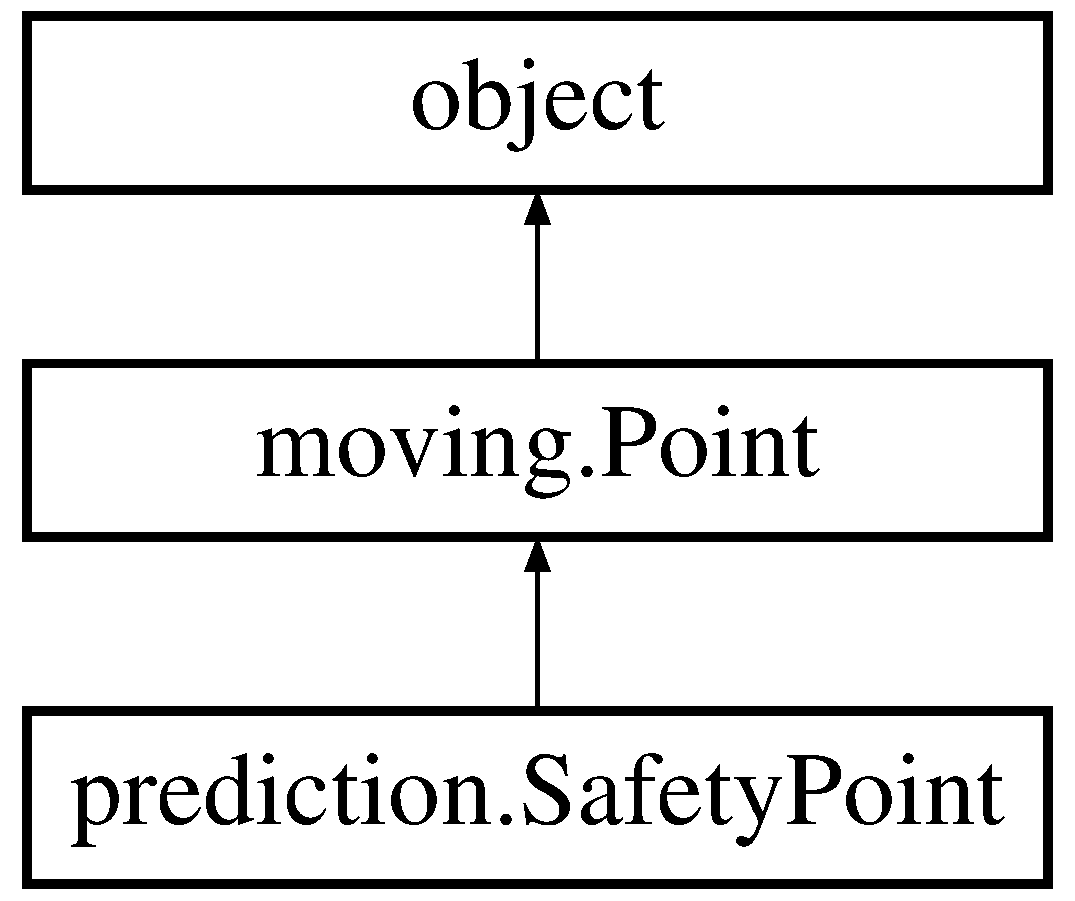
\includegraphics[height=3.000000cm]{classmoving_1_1Point}
\end{center}
\end{figure}
\subsubsection*{Public Member Functions}
\begin{DoxyCompactItemize}
\item 
def \hyperlink{classmoving_1_1Point_a44fc2d3b55f809577f3a6bb682e2ac5a}{\-\_\-\-\_\-init\-\_\-\-\_\-}
\item 
def \hyperlink{classmoving_1_1Point_a4aeb02318ecf00cd139bb2690c5fb8d2}{\-\_\-\-\_\-str\-\_\-\-\_\-}
\item 
def \hyperlink{classmoving_1_1Point_a61d7f277059d4f876f2f63af6ebaf122}{\-\_\-\-\_\-repr\-\_\-\-\_\-}
\item 
def \hyperlink{classmoving_1_1Point_a1e7a55f11fc6bd0ff3d25794933aee16}{\-\_\-\-\_\-add\-\_\-\-\_\-}
\item 
def \hyperlink{classmoving_1_1Point_aee55a8400abb5b4aaf1b0b1deceef2fe}{\-\_\-\-\_\-sub\-\_\-\-\_\-}
\item 
def \hyperlink{classmoving_1_1Point_a1a5018439473fe5c295245e022f0682e}{\-\_\-\-\_\-neg\-\_\-\-\_\-}
\item 
def \hyperlink{classmoving_1_1Point_a7ab2de1feab8f960cd963352f57e047e}{\-\_\-\-\_\-getitem\-\_\-\-\_\-}
\item 
def \hyperlink{classmoving_1_1Point_a89770895dc0dc2dbea37104a8500bc26}{orthogonal}
\item 
def \hyperlink{classmoving_1_1Point_ad5cbbe55eb76ed3c749cd431955ff0ad}{multiply}
\item 
def \hyperlink{classmoving_1_1Point_a4f37011f7c4a200e52d8278d44a093dc}{divide}
\item 
def \hyperlink{classmoving_1_1Point_a6eeb0e3d7ed0425614b8c95cee2a6235}{plot}
\item 
def \hyperlink{classmoving_1_1Point_adbf64130bc95de49330a03fbac10fb66}{norm2\-Squared}
\item 
def \hyperlink{classmoving_1_1Point_a6c886e2c4036aa68e4128a49269cf0d3}{norm2}
\item 
def \hyperlink{classmoving_1_1Point_a217a1b9694d93310381337ac8360bb91}{norm1}
\item 
def \hyperlink{classmoving_1_1Point_ae3975fff4392ed5d3eff3f366e7b2203}{norm\-Max}
\item 
def \hyperlink{classmoving_1_1Point_a84443e6f0f9c93a91d7b0a9c3ad2b8ca}{aslist}
\item 
def \hyperlink{classmoving_1_1Point_adf4eefc6393071a3b2381e7604abd742}{astuple}
\item 
def \hyperlink{classmoving_1_1Point_acaedde5a5de00853cd4c0cad4d58e42d}{asint}
\item 
def \hyperlink{classmoving_1_1Point_a51a718adc29d293ea0747287f3e21332}{as\-Shapely}
\item 
def \hyperlink{classmoving_1_1Point_ab113bf45dca9c7ef476e771a0f398538}{project}
\item 
def \hyperlink{classmoving_1_1Point_a72eb10d472f2c5d2af3362f9e82d65ba}{in\-Polygon}
\item 
def \hyperlink{classmoving_1_1Point_a932d2589d44ab0404b0df32e29b28332}{similar\-Orientation}
\end{DoxyCompactItemize}
\subsubsection*{Static Public Member Functions}
\begin{DoxyCompactItemize}
\item 
def \hyperlink{classmoving_1_1Point_a0eca4279233621a49058128cf49d268e}{from\-List}
\item 
def \hyperlink{classmoving_1_1Point_a1125de99473e70b5e623afa35380ef85}{dot}
\item 
def \hyperlink{classmoving_1_1Point_ad55fe85b7eb400c0848950c235b657c1}{cross}
\item 
def \hyperlink{classmoving_1_1Point_a3b09889b4479529b9b229fa6a6a5c10a}{cosine}
\item 
def \hyperlink{classmoving_1_1Point_a980a284b4a616596e329f55d88d95da9}{distance\-Norm2}
\item 
def \hyperlink{classmoving_1_1Point_a0f26390e9225b13f3c59391a3984541d}{plot\-All}
\item 
def \hyperlink{classmoving_1_1Point_a76045bf736f89d85bfa71d4a0235f989}{time\-To\-Collision}
\item 
def \hyperlink{classmoving_1_1Point_a1f759364011b39b62b0e1e6290169d92}{mid\-Point}
\end{DoxyCompactItemize}
\subsubsection*{Public Attributes}
\begin{DoxyCompactItemize}
\item 
\hyperlink{classmoving_1_1Point_ab402f7831ffa4f4398b90819496126ad}{x}
\item 
\hyperlink{classmoving_1_1Point_ae812508e0663bded8b2be4fc0b3584ff}{y}
\end{DoxyCompactItemize}


\subsubsection{Constructor \& Destructor Documentation}
\hypertarget{classmoving_1_1Point_a44fc2d3b55f809577f3a6bb682e2ac5a}{\index{moving\-::\-Point@{moving\-::\-Point}!\-\_\-\-\_\-init\-\_\-\-\_\-@{\-\_\-\-\_\-init\-\_\-\-\_\-}}
\index{\-\_\-\-\_\-init\-\_\-\-\_\-@{\-\_\-\-\_\-init\-\_\-\-\_\-}!moving::Point@{moving\-::\-Point}}
\paragraph[{\-\_\-\-\_\-init\-\_\-\-\_\-}]{\setlength{\rightskip}{0pt plus 5cm}def moving.\-Point.\-\_\-\-\_\-init\-\_\-\-\_\- (
\begin{DoxyParamCaption}
\item[{}]{self, }
\item[{}]{x, }
\item[{}]{y}
\end{DoxyParamCaption}
)}}\label{classmoving_1_1Point_a44fc2d3b55f809577f3a6bb682e2ac5a}


\subsubsection{Member Function Documentation}
\hypertarget{classmoving_1_1Point_a1e7a55f11fc6bd0ff3d25794933aee16}{\index{moving\-::\-Point@{moving\-::\-Point}!\-\_\-\-\_\-add\-\_\-\-\_\-@{\-\_\-\-\_\-add\-\_\-\-\_\-}}
\index{\-\_\-\-\_\-add\-\_\-\-\_\-@{\-\_\-\-\_\-add\-\_\-\-\_\-}!moving::Point@{moving\-::\-Point}}
\paragraph[{\-\_\-\-\_\-add\-\_\-\-\_\-}]{\setlength{\rightskip}{0pt plus 5cm}def moving.\-Point.\-\_\-\-\_\-add\-\_\-\-\_\- (
\begin{DoxyParamCaption}
\item[{}]{self, }
\item[{}]{other}
\end{DoxyParamCaption}
)}}\label{classmoving_1_1Point_a1e7a55f11fc6bd0ff3d25794933aee16}


References metadata.\-Point.\-x, moving.\-Point.\-x, metadata.\-Point.\-y, and moving.\-Point.\-y.

\hypertarget{classmoving_1_1Point_a7ab2de1feab8f960cd963352f57e047e}{\index{moving\-::\-Point@{moving\-::\-Point}!\-\_\-\-\_\-getitem\-\_\-\-\_\-@{\-\_\-\-\_\-getitem\-\_\-\-\_\-}}
\index{\-\_\-\-\_\-getitem\-\_\-\-\_\-@{\-\_\-\-\_\-getitem\-\_\-\-\_\-}!moving::Point@{moving\-::\-Point}}
\paragraph[{\-\_\-\-\_\-getitem\-\_\-\-\_\-}]{\setlength{\rightskip}{0pt plus 5cm}def moving.\-Point.\-\_\-\-\_\-getitem\-\_\-\-\_\- (
\begin{DoxyParamCaption}
\item[{}]{self, }
\item[{}]{i}
\end{DoxyParamCaption}
)}}\label{classmoving_1_1Point_a7ab2de1feab8f960cd963352f57e047e}


References metadata.\-Point.\-x, moving.\-Point.\-x, metadata.\-Point.\-y, and moving.\-Point.\-y.

\hypertarget{classmoving_1_1Point_a1a5018439473fe5c295245e022f0682e}{\index{moving\-::\-Point@{moving\-::\-Point}!\-\_\-\-\_\-neg\-\_\-\-\_\-@{\-\_\-\-\_\-neg\-\_\-\-\_\-}}
\index{\-\_\-\-\_\-neg\-\_\-\-\_\-@{\-\_\-\-\_\-neg\-\_\-\-\_\-}!moving::Point@{moving\-::\-Point}}
\paragraph[{\-\_\-\-\_\-neg\-\_\-\-\_\-}]{\setlength{\rightskip}{0pt plus 5cm}def moving.\-Point.\-\_\-\-\_\-neg\-\_\-\-\_\- (
\begin{DoxyParamCaption}
\item[{}]{self}
\end{DoxyParamCaption}
)}}\label{classmoving_1_1Point_a1a5018439473fe5c295245e022f0682e}


References metadata.\-Point.\-x, moving.\-Point.\-x, metadata.\-Point.\-y, and moving.\-Point.\-y.

\hypertarget{classmoving_1_1Point_a61d7f277059d4f876f2f63af6ebaf122}{\index{moving\-::\-Point@{moving\-::\-Point}!\-\_\-\-\_\-repr\-\_\-\-\_\-@{\-\_\-\-\_\-repr\-\_\-\-\_\-}}
\index{\-\_\-\-\_\-repr\-\_\-\-\_\-@{\-\_\-\-\_\-repr\-\_\-\-\_\-}!moving::Point@{moving\-::\-Point}}
\paragraph[{\-\_\-\-\_\-repr\-\_\-\-\_\-}]{\setlength{\rightskip}{0pt plus 5cm}def moving.\-Point.\-\_\-\-\_\-repr\-\_\-\-\_\- (
\begin{DoxyParamCaption}
\item[{}]{self}
\end{DoxyParamCaption}
)}}\label{classmoving_1_1Point_a61d7f277059d4f876f2f63af6ebaf122}


References moving.\-Interval.\-\_\-\-\_\-str\-\_\-\-\_\-(), and moving.\-Point.\-\_\-\-\_\-str\-\_\-\-\_\-().

\hypertarget{classmoving_1_1Point_a4aeb02318ecf00cd139bb2690c5fb8d2}{\index{moving\-::\-Point@{moving\-::\-Point}!\-\_\-\-\_\-str\-\_\-\-\_\-@{\-\_\-\-\_\-str\-\_\-\-\_\-}}
\index{\-\_\-\-\_\-str\-\_\-\-\_\-@{\-\_\-\-\_\-str\-\_\-\-\_\-}!moving::Point@{moving\-::\-Point}}
\paragraph[{\-\_\-\-\_\-str\-\_\-\-\_\-}]{\setlength{\rightskip}{0pt plus 5cm}def moving.\-Point.\-\_\-\-\_\-str\-\_\-\-\_\- (
\begin{DoxyParamCaption}
\item[{}]{self}
\end{DoxyParamCaption}
)}}\label{classmoving_1_1Point_a4aeb02318ecf00cd139bb2690c5fb8d2}


References metadata.\-Point.\-x, moving.\-Point.\-x, metadata.\-Point.\-y, and moving.\-Point.\-y.

\hypertarget{classmoving_1_1Point_aee55a8400abb5b4aaf1b0b1deceef2fe}{\index{moving\-::\-Point@{moving\-::\-Point}!\-\_\-\-\_\-sub\-\_\-\-\_\-@{\-\_\-\-\_\-sub\-\_\-\-\_\-}}
\index{\-\_\-\-\_\-sub\-\_\-\-\_\-@{\-\_\-\-\_\-sub\-\_\-\-\_\-}!moving::Point@{moving\-::\-Point}}
\paragraph[{\-\_\-\-\_\-sub\-\_\-\-\_\-}]{\setlength{\rightskip}{0pt plus 5cm}def moving.\-Point.\-\_\-\-\_\-sub\-\_\-\-\_\- (
\begin{DoxyParamCaption}
\item[{}]{self, }
\item[{}]{other}
\end{DoxyParamCaption}
)}}\label{classmoving_1_1Point_aee55a8400abb5b4aaf1b0b1deceef2fe}


References metadata.\-Point.\-x, moving.\-Point.\-x, metadata.\-Point.\-y, and moving.\-Point.\-y.

\hypertarget{classmoving_1_1Point_acaedde5a5de00853cd4c0cad4d58e42d}{\index{moving\-::\-Point@{moving\-::\-Point}!asint@{asint}}
\index{asint@{asint}!moving::Point@{moving\-::\-Point}}
\paragraph[{asint}]{\setlength{\rightskip}{0pt plus 5cm}def moving.\-Point.\-asint (
\begin{DoxyParamCaption}
\item[{}]{self}
\end{DoxyParamCaption}
)}}\label{classmoving_1_1Point_acaedde5a5de00853cd4c0cad4d58e42d}


References metadata.\-Point.\-x, moving.\-Point.\-x, metadata.\-Point.\-y, and moving.\-Point.\-y.

\hypertarget{classmoving_1_1Point_a84443e6f0f9c93a91d7b0a9c3ad2b8ca}{\index{moving\-::\-Point@{moving\-::\-Point}!aslist@{aslist}}
\index{aslist@{aslist}!moving::Point@{moving\-::\-Point}}
\paragraph[{aslist}]{\setlength{\rightskip}{0pt plus 5cm}def moving.\-Point.\-aslist (
\begin{DoxyParamCaption}
\item[{}]{self}
\end{DoxyParamCaption}
)}}\label{classmoving_1_1Point_a84443e6f0f9c93a91d7b0a9c3ad2b8ca}


References metadata.\-Point.\-x, moving.\-Point.\-x, metadata.\-Point.\-y, and moving.\-Point.\-y.

\hypertarget{classmoving_1_1Point_a51a718adc29d293ea0747287f3e21332}{\index{moving\-::\-Point@{moving\-::\-Point}!as\-Shapely@{as\-Shapely}}
\index{as\-Shapely@{as\-Shapely}!moving::Point@{moving\-::\-Point}}
\paragraph[{as\-Shapely}]{\setlength{\rightskip}{0pt plus 5cm}def moving.\-Point.\-as\-Shapely (
\begin{DoxyParamCaption}
\item[{}]{self}
\end{DoxyParamCaption}
)}}\label{classmoving_1_1Point_a51a718adc29d293ea0747287f3e21332}


References metadata.\-Point.\-x, moving.\-Point.\-x, metadata.\-Point.\-y, and moving.\-Point.\-y.

\hypertarget{classmoving_1_1Point_adf4eefc6393071a3b2381e7604abd742}{\index{moving\-::\-Point@{moving\-::\-Point}!astuple@{astuple}}
\index{astuple@{astuple}!moving::Point@{moving\-::\-Point}}
\paragraph[{astuple}]{\setlength{\rightskip}{0pt plus 5cm}def moving.\-Point.\-astuple (
\begin{DoxyParamCaption}
\item[{}]{self}
\end{DoxyParamCaption}
)}}\label{classmoving_1_1Point_adf4eefc6393071a3b2381e7604abd742}


References metadata.\-Point.\-x, moving.\-Point.\-x, metadata.\-Point.\-y, and moving.\-Point.\-y.

\hypertarget{classmoving_1_1Point_a3b09889b4479529b9b229fa6a6a5c10a}{\index{moving\-::\-Point@{moving\-::\-Point}!cosine@{cosine}}
\index{cosine@{cosine}!moving::Point@{moving\-::\-Point}}
\paragraph[{cosine}]{\setlength{\rightskip}{0pt plus 5cm}def moving.\-Point.\-cosine (
\begin{DoxyParamCaption}
\item[{}]{p1, }
\item[{}]{p2}
\end{DoxyParamCaption}
)\hspace{0.3cm}{\ttfamily [static]}}}\label{classmoving_1_1Point_a3b09889b4479529b9b229fa6a6a5c10a}
\hypertarget{classmoving_1_1Point_ad55fe85b7eb400c0848950c235b657c1}{\index{moving\-::\-Point@{moving\-::\-Point}!cross@{cross}}
\index{cross@{cross}!moving::Point@{moving\-::\-Point}}
\paragraph[{cross}]{\setlength{\rightskip}{0pt plus 5cm}def moving.\-Point.\-cross (
\begin{DoxyParamCaption}
\item[{}]{p1, }
\item[{}]{p2}
\end{DoxyParamCaption}
)\hspace{0.3cm}{\ttfamily [static]}}}\label{classmoving_1_1Point_ad55fe85b7eb400c0848950c235b657c1}
\hypertarget{classmoving_1_1Point_a980a284b4a616596e329f55d88d95da9}{\index{moving\-::\-Point@{moving\-::\-Point}!distance\-Norm2@{distance\-Norm2}}
\index{distance\-Norm2@{distance\-Norm2}!moving::Point@{moving\-::\-Point}}
\paragraph[{distance\-Norm2}]{\setlength{\rightskip}{0pt plus 5cm}def moving.\-Point.\-distance\-Norm2 (
\begin{DoxyParamCaption}
\item[{}]{p1, }
\item[{}]{p2}
\end{DoxyParamCaption}
)\hspace{0.3cm}{\ttfamily [static]}}}\label{classmoving_1_1Point_a980a284b4a616596e329f55d88d95da9}


References moving.\-Point.\-norm2().

\hypertarget{classmoving_1_1Point_a4f37011f7c4a200e52d8278d44a093dc}{\index{moving\-::\-Point@{moving\-::\-Point}!divide@{divide}}
\index{divide@{divide}!moving::Point@{moving\-::\-Point}}
\paragraph[{divide}]{\setlength{\rightskip}{0pt plus 5cm}def moving.\-Point.\-divide (
\begin{DoxyParamCaption}
\item[{}]{self, }
\item[{}]{alpha}
\end{DoxyParamCaption}
)}}\label{classmoving_1_1Point_a4f37011f7c4a200e52d8278d44a093dc}


References metadata.\-Point.\-x, moving.\-Point.\-x, metadata.\-Point.\-y, and moving.\-Point.\-y.

\hypertarget{classmoving_1_1Point_a1125de99473e70b5e623afa35380ef85}{\index{moving\-::\-Point@{moving\-::\-Point}!dot@{dot}}
\index{dot@{dot}!moving::Point@{moving\-::\-Point}}
\paragraph[{dot}]{\setlength{\rightskip}{0pt plus 5cm}def moving.\-Point.\-dot (
\begin{DoxyParamCaption}
\item[{}]{p1, }
\item[{}]{p2}
\end{DoxyParamCaption}
)\hspace{0.3cm}{\ttfamily [static]}}}\label{classmoving_1_1Point_a1125de99473e70b5e623afa35380ef85}
\hypertarget{classmoving_1_1Point_a0eca4279233621a49058128cf49d268e}{\index{moving\-::\-Point@{moving\-::\-Point}!from\-List@{from\-List}}
\index{from\-List@{from\-List}!moving::Point@{moving\-::\-Point}}
\paragraph[{from\-List}]{\setlength{\rightskip}{0pt plus 5cm}def moving.\-Point.\-from\-List (
\begin{DoxyParamCaption}
\item[{}]{p}
\end{DoxyParamCaption}
)\hspace{0.3cm}{\ttfamily [static]}}}\label{classmoving_1_1Point_a0eca4279233621a49058128cf49d268e}
\hypertarget{classmoving_1_1Point_a72eb10d472f2c5d2af3362f9e82d65ba}{\index{moving\-::\-Point@{moving\-::\-Point}!in\-Polygon@{in\-Polygon}}
\index{in\-Polygon@{in\-Polygon}!moving::Point@{moving\-::\-Point}}
\paragraph[{in\-Polygon}]{\setlength{\rightskip}{0pt plus 5cm}def moving.\-Point.\-in\-Polygon (
\begin{DoxyParamCaption}
\item[{}]{self, }
\item[{}]{polygon}
\end{DoxyParamCaption}
)}}\label{classmoving_1_1Point_a72eb10d472f2c5d2af3362f9e82d65ba}
\begin{DoxyVerb}Indicates if the point x, y is inside the polygon
(array of Nx2 coordinates of the polygon vertices)

taken from http://www.ariel.com.au/a/python-point-int-poly.html

Use Polygon.contains if Shapely is installed\end{DoxyVerb}
 

References metadata.\-Point.\-x, moving.\-Point.\-x, metadata.\-Point.\-y, and moving.\-Point.\-y.

\hypertarget{classmoving_1_1Point_a1f759364011b39b62b0e1e6290169d92}{\index{moving\-::\-Point@{moving\-::\-Point}!mid\-Point@{mid\-Point}}
\index{mid\-Point@{mid\-Point}!moving::Point@{moving\-::\-Point}}
\paragraph[{mid\-Point}]{\setlength{\rightskip}{0pt plus 5cm}def moving.\-Point.\-mid\-Point (
\begin{DoxyParamCaption}
\item[{}]{p1, }
\item[{}]{p2}
\end{DoxyParamCaption}
)\hspace{0.3cm}{\ttfamily [static]}}}\label{classmoving_1_1Point_a1f759364011b39b62b0e1e6290169d92}
\hypertarget{classmoving_1_1Point_ad5cbbe55eb76ed3c749cd431955ff0ad}{\index{moving\-::\-Point@{moving\-::\-Point}!multiply@{multiply}}
\index{multiply@{multiply}!moving::Point@{moving\-::\-Point}}
\paragraph[{multiply}]{\setlength{\rightskip}{0pt plus 5cm}def moving.\-Point.\-multiply (
\begin{DoxyParamCaption}
\item[{}]{self, }
\item[{}]{alpha}
\end{DoxyParamCaption}
)}}\label{classmoving_1_1Point_ad5cbbe55eb76ed3c749cd431955ff0ad}


References metadata.\-Point.\-x, moving.\-Point.\-x, metadata.\-Point.\-y, and moving.\-Point.\-y.

\hypertarget{classmoving_1_1Point_a217a1b9694d93310381337ac8360bb91}{\index{moving\-::\-Point@{moving\-::\-Point}!norm1@{norm1}}
\index{norm1@{norm1}!moving::Point@{moving\-::\-Point}}
\paragraph[{norm1}]{\setlength{\rightskip}{0pt plus 5cm}def moving.\-Point.\-norm1 (
\begin{DoxyParamCaption}
\item[{}]{self}
\end{DoxyParamCaption}
)}}\label{classmoving_1_1Point_a217a1b9694d93310381337ac8360bb91}


References metadata.\-Point.\-x, moving.\-Point.\-x, metadata.\-Point.\-y, and moving.\-Point.\-y.

\hypertarget{classmoving_1_1Point_a6c886e2c4036aa68e4128a49269cf0d3}{\index{moving\-::\-Point@{moving\-::\-Point}!norm2@{norm2}}
\index{norm2@{norm2}!moving::Point@{moving\-::\-Point}}
\paragraph[{norm2}]{\setlength{\rightskip}{0pt plus 5cm}def moving.\-Point.\-norm2 (
\begin{DoxyParamCaption}
\item[{}]{self}
\end{DoxyParamCaption}
)}}\label{classmoving_1_1Point_a6c886e2c4036aa68e4128a49269cf0d3}
\begin{DoxyVerb}2-norm distance (Euclidean distance)\end{DoxyVerb}
 

References moving.\-Point.\-norm2\-Squared().

\hypertarget{classmoving_1_1Point_adbf64130bc95de49330a03fbac10fb66}{\index{moving\-::\-Point@{moving\-::\-Point}!norm2\-Squared@{norm2\-Squared}}
\index{norm2\-Squared@{norm2\-Squared}!moving::Point@{moving\-::\-Point}}
\paragraph[{norm2\-Squared}]{\setlength{\rightskip}{0pt plus 5cm}def moving.\-Point.\-norm2\-Squared (
\begin{DoxyParamCaption}
\item[{}]{self}
\end{DoxyParamCaption}
)}}\label{classmoving_1_1Point_adbf64130bc95de49330a03fbac10fb66}
\begin{DoxyVerb}2-norm distance (Euclidean distance)\end{DoxyVerb}
 

References metadata.\-Point.\-x, moving.\-Point.\-x, metadata.\-Point.\-y, and moving.\-Point.\-y.

\hypertarget{classmoving_1_1Point_ae3975fff4392ed5d3eff3f366e7b2203}{\index{moving\-::\-Point@{moving\-::\-Point}!norm\-Max@{norm\-Max}}
\index{norm\-Max@{norm\-Max}!moving::Point@{moving\-::\-Point}}
\paragraph[{norm\-Max}]{\setlength{\rightskip}{0pt plus 5cm}def moving.\-Point.\-norm\-Max (
\begin{DoxyParamCaption}
\item[{}]{self}
\end{DoxyParamCaption}
)}}\label{classmoving_1_1Point_ae3975fff4392ed5d3eff3f366e7b2203}


References metadata.\-Point.\-x, moving.\-Point.\-x, metadata.\-Point.\-y, and moving.\-Point.\-y.

\hypertarget{classmoving_1_1Point_a89770895dc0dc2dbea37104a8500bc26}{\index{moving\-::\-Point@{moving\-::\-Point}!orthogonal@{orthogonal}}
\index{orthogonal@{orthogonal}!moving::Point@{moving\-::\-Point}}
\paragraph[{orthogonal}]{\setlength{\rightskip}{0pt plus 5cm}def moving.\-Point.\-orthogonal (
\begin{DoxyParamCaption}
\item[{}]{self, }
\item[{}]{clockwise = {\ttfamily True}}
\end{DoxyParamCaption}
)}}\label{classmoving_1_1Point_a89770895dc0dc2dbea37104a8500bc26}


References metadata.\-Point.\-x, moving.\-Point.\-x, metadata.\-Point.\-y, and moving.\-Point.\-y.

\hypertarget{classmoving_1_1Point_a6eeb0e3d7ed0425614b8c95cee2a6235}{\index{moving\-::\-Point@{moving\-::\-Point}!plot@{plot}}
\index{plot@{plot}!moving::Point@{moving\-::\-Point}}
\paragraph[{plot}]{\setlength{\rightskip}{0pt plus 5cm}def moving.\-Point.\-plot (
\begin{DoxyParamCaption}
\item[{}]{self, }
\item[{}]{options = {\ttfamily 'o'}, }
\item[{}]{kwargs}
\end{DoxyParamCaption}
)}}\label{classmoving_1_1Point_a6eeb0e3d7ed0425614b8c95cee2a6235}


References metadata.\-Point.\-x, moving.\-Point.\-x, metadata.\-Point.\-y, and moving.\-Point.\-y.

\hypertarget{classmoving_1_1Point_a0f26390e9225b13f3c59391a3984541d}{\index{moving\-::\-Point@{moving\-::\-Point}!plot\-All@{plot\-All}}
\index{plot\-All@{plot\-All}!moving::Point@{moving\-::\-Point}}
\paragraph[{plot\-All}]{\setlength{\rightskip}{0pt plus 5cm}def moving.\-Point.\-plot\-All (
\begin{DoxyParamCaption}
\item[{}]{points, }
\item[{}]{kwargs}
\end{DoxyParamCaption}
)\hspace{0.3cm}{\ttfamily [static]}}}\label{classmoving_1_1Point_a0f26390e9225b13f3c59391a3984541d}
\hypertarget{classmoving_1_1Point_ab113bf45dca9c7ef476e771a0f398538}{\index{moving\-::\-Point@{moving\-::\-Point}!project@{project}}
\index{project@{project}!moving::Point@{moving\-::\-Point}}
\paragraph[{project}]{\setlength{\rightskip}{0pt plus 5cm}def moving.\-Point.\-project (
\begin{DoxyParamCaption}
\item[{}]{self, }
\item[{}]{homography}
\end{DoxyParamCaption}
)}}\label{classmoving_1_1Point_ab113bf45dca9c7ef476e771a0f398538}


References cvutils.\-project\-Array(), metadata.\-Point.\-x, moving.\-Point.\-x, metadata.\-Point.\-y, and moving.\-Point.\-y.

\hypertarget{classmoving_1_1Point_a932d2589d44ab0404b0df32e29b28332}{\index{moving\-::\-Point@{moving\-::\-Point}!similar\-Orientation@{similar\-Orientation}}
\index{similar\-Orientation@{similar\-Orientation}!moving::Point@{moving\-::\-Point}}
\paragraph[{similar\-Orientation}]{\setlength{\rightskip}{0pt plus 5cm}def moving.\-Point.\-similar\-Orientation (
\begin{DoxyParamCaption}
\item[{}]{self, }
\item[{}]{ref\-Direction, }
\item[{}]{cosine\-Threshold}
\end{DoxyParamCaption}
)}}\label{classmoving_1_1Point_a932d2589d44ab0404b0df32e29b28332}
\hypertarget{classmoving_1_1Point_a76045bf736f89d85bfa71d4a0235f989}{\index{moving\-::\-Point@{moving\-::\-Point}!time\-To\-Collision@{time\-To\-Collision}}
\index{time\-To\-Collision@{time\-To\-Collision}!moving::Point@{moving\-::\-Point}}
\paragraph[{time\-To\-Collision}]{\setlength{\rightskip}{0pt plus 5cm}def moving.\-Point.\-time\-To\-Collision (
\begin{DoxyParamCaption}
\item[{}]{p1, }
\item[{}]{p2, }
\item[{}]{v1, }
\item[{}]{v2, }
\item[{}]{collision\-Threshold}
\end{DoxyParamCaption}
)\hspace{0.3cm}{\ttfamily [static]}}}\label{classmoving_1_1Point_a76045bf736f89d85bfa71d4a0235f989}
\begin{DoxyVerb}Computes exact time to collision with a distance threshold
The unknown of the equation is the time to reach the intersection
between the relative trajectory of one road user
and the circle of radius collisionThreshold around the other road user\end{DoxyVerb}
 

\subsubsection{Member Data Documentation}
\hypertarget{classmoving_1_1Point_ab402f7831ffa4f4398b90819496126ad}{\index{moving\-::\-Point@{moving\-::\-Point}!x@{x}}
\index{x@{x}!moving::Point@{moving\-::\-Point}}
\paragraph[{x}]{\setlength{\rightskip}{0pt plus 5cm}moving.\-Point.\-x}}\label{classmoving_1_1Point_ab402f7831ffa4f4398b90819496126ad}
\hypertarget{classmoving_1_1Point_ae812508e0663bded8b2be4fc0b3584ff}{\index{moving\-::\-Point@{moving\-::\-Point}!y@{y}}
\index{y@{y}!moving::Point@{moving\-::\-Point}}
\paragraph[{y}]{\setlength{\rightskip}{0pt plus 5cm}moving.\-Point.\-y}}\label{classmoving_1_1Point_ae812508e0663bded8b2be4fc0b3584ff}


The documentation for this class was generated from the following file\-:\begin{DoxyCompactItemize}
\item 
python/\hyperlink{moving_8py}{moving.\-py}\end{DoxyCompactItemize}

\hypertarget{classprediction_1_1PointSetPredictionParameters}{\subsection{prediction.\-Point\-Set\-Prediction\-Parameters Class Reference}
\label{classprediction_1_1PointSetPredictionParameters}\index{prediction.\-Point\-Set\-Prediction\-Parameters@{prediction.\-Point\-Set\-Prediction\-Parameters}}
}
Inheritance diagram for prediction.\-Point\-Set\-Prediction\-Parameters\-:\begin{figure}[H]
\begin{center}
\leavevmode
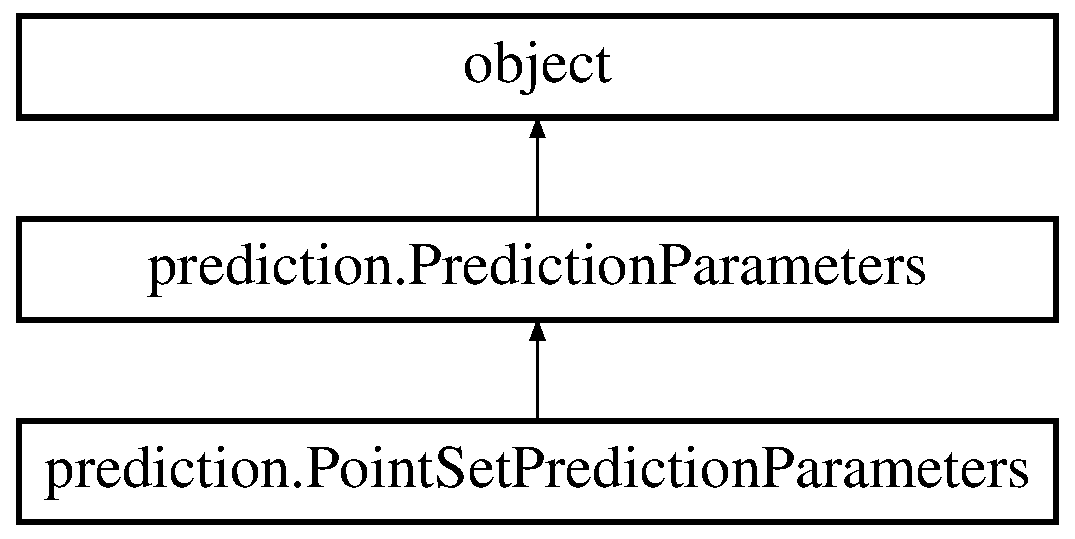
\includegraphics[height=3.000000cm]{classprediction_1_1PointSetPredictionParameters}
\end{center}
\end{figure}
\subsubsection*{Public Member Functions}
\begin{DoxyCompactItemize}
\item 
def \hyperlink{classprediction_1_1PointSetPredictionParameters_af1dc00ac92be1ac2c1a4c0b3359f9f70}{\-\_\-\-\_\-init\-\_\-\-\_\-}
\item 
def \hyperlink{classprediction_1_1PointSetPredictionParameters_a86abb08ab71d587c8447692f722b4831}{generate\-Predicted\-Trajectories}
\end{DoxyCompactItemize}
\subsubsection*{Additional Inherited Members}


\subsubsection{Constructor \& Destructor Documentation}
\hypertarget{classprediction_1_1PointSetPredictionParameters_af1dc00ac92be1ac2c1a4c0b3359f9f70}{\index{prediction\-::\-Point\-Set\-Prediction\-Parameters@{prediction\-::\-Point\-Set\-Prediction\-Parameters}!\-\_\-\-\_\-init\-\_\-\-\_\-@{\-\_\-\-\_\-init\-\_\-\-\_\-}}
\index{\-\_\-\-\_\-init\-\_\-\-\_\-@{\-\_\-\-\_\-init\-\_\-\-\_\-}!prediction::PointSetPredictionParameters@{prediction\-::\-Point\-Set\-Prediction\-Parameters}}
\paragraph[{\-\_\-\-\_\-init\-\_\-\-\_\-}]{\setlength{\rightskip}{0pt plus 5cm}def prediction.\-Point\-Set\-Prediction\-Parameters.\-\_\-\-\_\-init\-\_\-\-\_\- (
\begin{DoxyParamCaption}
\item[{}]{self, }
\item[{}]{max\-Speed}
\end{DoxyParamCaption}
)}}\label{classprediction_1_1PointSetPredictionParameters_af1dc00ac92be1ac2c1a4c0b3359f9f70}


\subsubsection{Member Function Documentation}
\hypertarget{classprediction_1_1PointSetPredictionParameters_a86abb08ab71d587c8447692f722b4831}{\index{prediction\-::\-Point\-Set\-Prediction\-Parameters@{prediction\-::\-Point\-Set\-Prediction\-Parameters}!generate\-Predicted\-Trajectories@{generate\-Predicted\-Trajectories}}
\index{generate\-Predicted\-Trajectories@{generate\-Predicted\-Trajectories}!prediction::PointSetPredictionParameters@{prediction\-::\-Point\-Set\-Prediction\-Parameters}}
\paragraph[{generate\-Predicted\-Trajectories}]{\setlength{\rightskip}{0pt plus 5cm}def prediction.\-Point\-Set\-Prediction\-Parameters.\-generate\-Predicted\-Trajectories (
\begin{DoxyParamCaption}
\item[{}]{self, }
\item[{}]{obj, }
\item[{}]{instant}
\end{DoxyParamCaption}
)}}\label{classprediction_1_1PointSetPredictionParameters_a86abb08ab71d587c8447692f722b4831}


References prediction.\-Predicted\-Trajectory\-Constant.\-max\-Speed, prediction.\-Predicted\-Trajectory\-Random\-Control.\-max\-Speed, and prediction.\-Prediction\-Parameters.\-max\-Speed.



The documentation for this class was generated from the following file\-:\begin{DoxyCompactItemize}
\item 
python/\hyperlink{prediction_8py}{prediction.\-py}\end{DoxyCompactItemize}

\hypertarget{classprediction_1_1PredictedTrajectory}{\subsection{prediction.\-Predicted\-Trajectory Class Reference}
\label{classprediction_1_1PredictedTrajectory}\index{prediction.\-Predicted\-Trajectory@{prediction.\-Predicted\-Trajectory}}
}
Inheritance diagram for prediction.\-Predicted\-Trajectory\-:\begin{figure}[H]
\begin{center}
\leavevmode
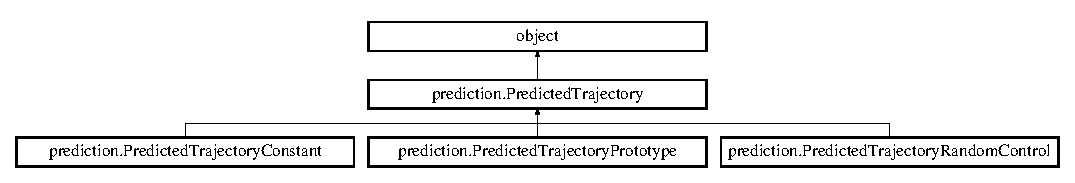
\includegraphics[height=2.014389cm]{classprediction_1_1PredictedTrajectory}
\end{center}
\end{figure}
\subsubsection*{Public Member Functions}
\begin{DoxyCompactItemize}
\item 
def \hyperlink{classprediction_1_1PredictedTrajectory_a74f7b7352274ba7694e4a9b76b68d653}{\-\_\-\-\_\-init\-\_\-\-\_\-}
\item 
def \hyperlink{classprediction_1_1PredictedTrajectory_a09f428bb05bd24b2e801d60634ae77a6}{predict\-Position}
\item 
def \hyperlink{classprediction_1_1PredictedTrajectory_adf34e5a664f07522310b049f452ce23c}{get\-Predicted\-Trajectory}
\item 
def \hyperlink{classprediction_1_1PredictedTrajectory_a17a313a577cb91c128a4c07f5df45115}{get\-Predicted\-Speeds}
\item 
def \hyperlink{classprediction_1_1PredictedTrajectory_a407d4824af1ecef642afaa797ded04d3}{plot}
\end{DoxyCompactItemize}
\subsubsection*{Public Attributes}
\begin{DoxyCompactItemize}
\item 
\hyperlink{classprediction_1_1PredictedTrajectory_a6f9fdfc40bf0256bf4b1574aebef5819}{probability}
\item 
\hyperlink{classprediction_1_1PredictedTrajectory_aab0c8a175ad11b867c58a3537d1968a4}{predicted\-Positions}
\item 
\hyperlink{classprediction_1_1PredictedTrajectory_aa190da0abcda7865e5d5dfbe9ba162b5}{predicted\-Speed\-Orientations}
\end{DoxyCompactItemize}


\subsubsection{Detailed Description}
\begin{DoxyVerb}Class for predicted trajectories with lazy evaluation
if the predicted position has not been already computed, compute it

it should also have a probability\end{DoxyVerb}
 

\subsubsection{Constructor \& Destructor Documentation}
\hypertarget{classprediction_1_1PredictedTrajectory_a74f7b7352274ba7694e4a9b76b68d653}{\index{prediction\-::\-Predicted\-Trajectory@{prediction\-::\-Predicted\-Trajectory}!\-\_\-\-\_\-init\-\_\-\-\_\-@{\-\_\-\-\_\-init\-\_\-\-\_\-}}
\index{\-\_\-\-\_\-init\-\_\-\-\_\-@{\-\_\-\-\_\-init\-\_\-\-\_\-}!prediction::PredictedTrajectory@{prediction\-::\-Predicted\-Trajectory}}
\paragraph[{\-\_\-\-\_\-init\-\_\-\-\_\-}]{\setlength{\rightskip}{0pt plus 5cm}def prediction.\-Predicted\-Trajectory.\-\_\-\-\_\-init\-\_\-\-\_\- (
\begin{DoxyParamCaption}
\item[{}]{self}
\end{DoxyParamCaption}
)}}\label{classprediction_1_1PredictedTrajectory_a74f7b7352274ba7694e4a9b76b68d653}


\subsubsection{Member Function Documentation}
\hypertarget{classprediction_1_1PredictedTrajectory_a17a313a577cb91c128a4c07f5df45115}{\index{prediction\-::\-Predicted\-Trajectory@{prediction\-::\-Predicted\-Trajectory}!get\-Predicted\-Speeds@{get\-Predicted\-Speeds}}
\index{get\-Predicted\-Speeds@{get\-Predicted\-Speeds}!prediction::PredictedTrajectory@{prediction\-::\-Predicted\-Trajectory}}
\paragraph[{get\-Predicted\-Speeds}]{\setlength{\rightskip}{0pt plus 5cm}def prediction.\-Predicted\-Trajectory.\-get\-Predicted\-Speeds (
\begin{DoxyParamCaption}
\item[{}]{self}
\end{DoxyParamCaption}
)}}\label{classprediction_1_1PredictedTrajectory_a17a313a577cb91c128a4c07f5df45115}
\hypertarget{classprediction_1_1PredictedTrajectory_adf34e5a664f07522310b049f452ce23c}{\index{prediction\-::\-Predicted\-Trajectory@{prediction\-::\-Predicted\-Trajectory}!get\-Predicted\-Trajectory@{get\-Predicted\-Trajectory}}
\index{get\-Predicted\-Trajectory@{get\-Predicted\-Trajectory}!prediction::PredictedTrajectory@{prediction\-::\-Predicted\-Trajectory}}
\paragraph[{get\-Predicted\-Trajectory}]{\setlength{\rightskip}{0pt plus 5cm}def prediction.\-Predicted\-Trajectory.\-get\-Predicted\-Trajectory (
\begin{DoxyParamCaption}
\item[{}]{self}
\end{DoxyParamCaption}
)}}\label{classprediction_1_1PredictedTrajectory_adf34e5a664f07522310b049f452ce23c}


References moving.\-Trajectory.\-from\-Point\-List().

\hypertarget{classprediction_1_1PredictedTrajectory_a407d4824af1ecef642afaa797ded04d3}{\index{prediction\-::\-Predicted\-Trajectory@{prediction\-::\-Predicted\-Trajectory}!plot@{plot}}
\index{plot@{plot}!prediction::PredictedTrajectory@{prediction\-::\-Predicted\-Trajectory}}
\paragraph[{plot}]{\setlength{\rightskip}{0pt plus 5cm}def prediction.\-Predicted\-Trajectory.\-plot (
\begin{DoxyParamCaption}
\item[{}]{self, }
\item[{}]{options = {\ttfamily ''}, }
\item[{}]{with\-Origin = {\ttfamily False}, }
\item[{}]{time\-Step = {\ttfamily 1}, }
\item[{}]{kwargs}
\end{DoxyParamCaption}
)}}\label{classprediction_1_1PredictedTrajectory_a407d4824af1ecef642afaa797ded04d3}


References prediction.\-Predicted\-Trajectory.\-get\-Predicted\-Trajectory().

\hypertarget{classprediction_1_1PredictedTrajectory_a09f428bb05bd24b2e801d60634ae77a6}{\index{prediction\-::\-Predicted\-Trajectory@{prediction\-::\-Predicted\-Trajectory}!predict\-Position@{predict\-Position}}
\index{predict\-Position@{predict\-Position}!prediction::PredictedTrajectory@{prediction\-::\-Predicted\-Trajectory}}
\paragraph[{predict\-Position}]{\setlength{\rightskip}{0pt plus 5cm}def prediction.\-Predicted\-Trajectory.\-predict\-Position (
\begin{DoxyParamCaption}
\item[{}]{self, }
\item[{}]{n\-Time\-Steps}
\end{DoxyParamCaption}
)}}\label{classprediction_1_1PredictedTrajectory_a09f428bb05bd24b2e801d60634ae77a6}


References prediction.\-Predicted\-Trajectory\-Constant.\-get\-Control(), prediction.\-Predicted\-Trajectory\-Random\-Control.\-get\-Control(), prediction.\-Predicted\-Trajectory\-Constant.\-max\-Speed, prediction.\-Predicted\-Trajectory\-Random\-Control.\-max\-Speed, prediction.\-Prediction\-Parameters.\-max\-Speed, prediction.\-Predicted\-Trajectory.\-predicted\-Positions, prediction.\-Predicted\-Trajectory.\-predicted\-Speed\-Orientations, prediction.\-Predicted\-Trajectory.\-predict\-Position(), moving.\-predict\-Position(), and moving.\-Moving\-Object.\-predict\-Position().



\subsubsection{Member Data Documentation}
\hypertarget{classprediction_1_1PredictedTrajectory_aab0c8a175ad11b867c58a3537d1968a4}{\index{prediction\-::\-Predicted\-Trajectory@{prediction\-::\-Predicted\-Trajectory}!predicted\-Positions@{predicted\-Positions}}
\index{predicted\-Positions@{predicted\-Positions}!prediction::PredictedTrajectory@{prediction\-::\-Predicted\-Trajectory}}
\paragraph[{predicted\-Positions}]{\setlength{\rightskip}{0pt plus 5cm}prediction.\-Predicted\-Trajectory.\-predicted\-Positions}}\label{classprediction_1_1PredictedTrajectory_aab0c8a175ad11b867c58a3537d1968a4}
\hypertarget{classprediction_1_1PredictedTrajectory_aa190da0abcda7865e5d5dfbe9ba162b5}{\index{prediction\-::\-Predicted\-Trajectory@{prediction\-::\-Predicted\-Trajectory}!predicted\-Speed\-Orientations@{predicted\-Speed\-Orientations}}
\index{predicted\-Speed\-Orientations@{predicted\-Speed\-Orientations}!prediction::PredictedTrajectory@{prediction\-::\-Predicted\-Trajectory}}
\paragraph[{predicted\-Speed\-Orientations}]{\setlength{\rightskip}{0pt plus 5cm}prediction.\-Predicted\-Trajectory.\-predicted\-Speed\-Orientations}}\label{classprediction_1_1PredictedTrajectory_aa190da0abcda7865e5d5dfbe9ba162b5}
\hypertarget{classprediction_1_1PredictedTrajectory_a6f9fdfc40bf0256bf4b1574aebef5819}{\index{prediction\-::\-Predicted\-Trajectory@{prediction\-::\-Predicted\-Trajectory}!probability@{probability}}
\index{probability@{probability}!prediction::PredictedTrajectory@{prediction\-::\-Predicted\-Trajectory}}
\paragraph[{probability}]{\setlength{\rightskip}{0pt plus 5cm}prediction.\-Predicted\-Trajectory.\-probability}}\label{classprediction_1_1PredictedTrajectory_a6f9fdfc40bf0256bf4b1574aebef5819}


The documentation for this class was generated from the following file\-:\begin{DoxyCompactItemize}
\item 
python/\hyperlink{prediction_8py}{prediction.\-py}\end{DoxyCompactItemize}

\hypertarget{classprediction_1_1PredictedTrajectoryConstant}{\subsection{prediction.\-Predicted\-Trajectory\-Constant Class Reference}
\label{classprediction_1_1PredictedTrajectoryConstant}\index{prediction.\-Predicted\-Trajectory\-Constant@{prediction.\-Predicted\-Trajectory\-Constant}}
}
Inheritance diagram for prediction.\-Predicted\-Trajectory\-Constant\-:\begin{figure}[H]
\begin{center}
\leavevmode
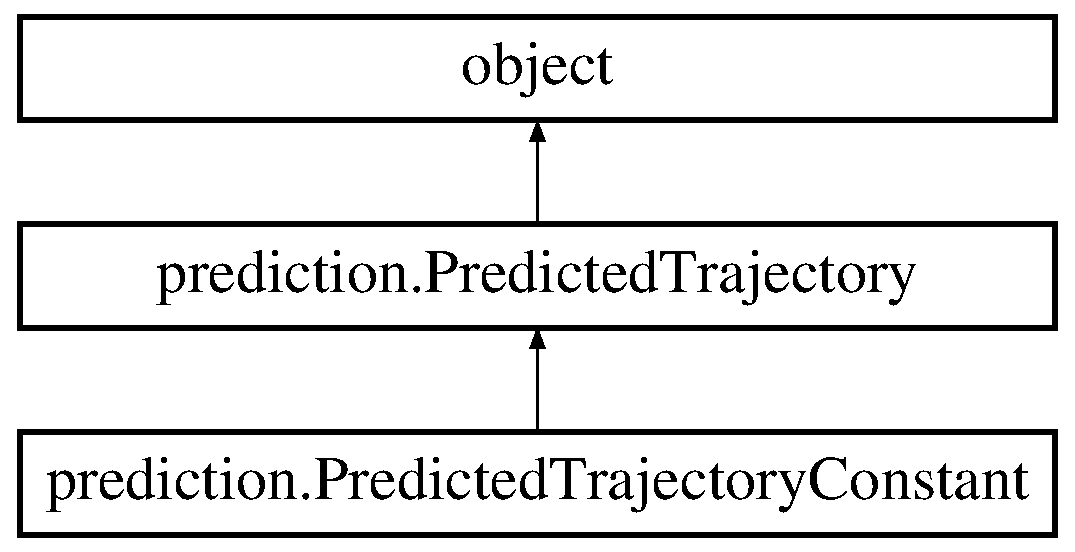
\includegraphics[height=3.000000cm]{classprediction_1_1PredictedTrajectoryConstant}
\end{center}
\end{figure}
\subsubsection*{Public Member Functions}
\begin{DoxyCompactItemize}
\item 
def \hyperlink{classprediction_1_1PredictedTrajectoryConstant_a722af0eeee7ea7ba8ecc7dce3dfd3612}{\-\_\-\-\_\-init\-\_\-\-\_\-}
\item 
def \hyperlink{classprediction_1_1PredictedTrajectoryConstant_a18acc110f76a332175721ac26c22485b}{get\-Control}
\end{DoxyCompactItemize}
\subsubsection*{Public Attributes}
\begin{DoxyCompactItemize}
\item 
\hyperlink{classprediction_1_1PredictedTrajectoryConstant_ae68f6314a9b1d1732cba734f5bf229a8}{control}
\item 
\hyperlink{classprediction_1_1PredictedTrajectoryConstant_a6b7055bfede1d9002344f749ba6e767d}{max\-Speed}
\item 
\hyperlink{classprediction_1_1PredictedTrajectoryConstant_a25a782bac3d4c5b57c76552c9b0fb34b}{probability}
\item 
\hyperlink{classprediction_1_1PredictedTrajectoryConstant_a539185ae508bef4837dff3b9c14932bf}{predicted\-Positions}
\item 
\hyperlink{classprediction_1_1PredictedTrajectoryConstant_af8a3f06e9bc93b447461dc952726b517}{predicted\-Speed\-Orientations}
\end{DoxyCompactItemize}


\subsubsection{Detailed Description}
\begin{DoxyVerb}Predicted trajectory at constant speed or acceleration
TODO generalize by passing a series of velocities/accelerations\end{DoxyVerb}
 

\subsubsection{Constructor \& Destructor Documentation}
\hypertarget{classprediction_1_1PredictedTrajectoryConstant_a722af0eeee7ea7ba8ecc7dce3dfd3612}{\index{prediction\-::\-Predicted\-Trajectory\-Constant@{prediction\-::\-Predicted\-Trajectory\-Constant}!\-\_\-\-\_\-init\-\_\-\-\_\-@{\-\_\-\-\_\-init\-\_\-\-\_\-}}
\index{\-\_\-\-\_\-init\-\_\-\-\_\-@{\-\_\-\-\_\-init\-\_\-\-\_\-}!prediction::PredictedTrajectoryConstant@{prediction\-::\-Predicted\-Trajectory\-Constant}}
\paragraph[{\-\_\-\-\_\-init\-\_\-\-\_\-}]{\setlength{\rightskip}{0pt plus 5cm}def prediction.\-Predicted\-Trajectory\-Constant.\-\_\-\-\_\-init\-\_\-\-\_\- (
\begin{DoxyParamCaption}
\item[{}]{self, }
\item[{}]{initial\-Position, }
\item[{}]{initial\-Velocity, }
\item[{}]{control = {\ttfamily {\bf moving.\-Norm\-Angle}(0,0}, }
\item[{}]{probability = {\ttfamily 1.}, }
\item[{}]{max\-Speed = {\ttfamily None}}
\end{DoxyParamCaption}
)}}\label{classprediction_1_1PredictedTrajectoryConstant_a722af0eeee7ea7ba8ecc7dce3dfd3612}


\subsubsection{Member Function Documentation}
\hypertarget{classprediction_1_1PredictedTrajectoryConstant_a18acc110f76a332175721ac26c22485b}{\index{prediction\-::\-Predicted\-Trajectory\-Constant@{prediction\-::\-Predicted\-Trajectory\-Constant}!get\-Control@{get\-Control}}
\index{get\-Control@{get\-Control}!prediction::PredictedTrajectoryConstant@{prediction\-::\-Predicted\-Trajectory\-Constant}}
\paragraph[{get\-Control}]{\setlength{\rightskip}{0pt plus 5cm}def prediction.\-Predicted\-Trajectory\-Constant.\-get\-Control (
\begin{DoxyParamCaption}
\item[{}]{self}
\end{DoxyParamCaption}
)}}\label{classprediction_1_1PredictedTrajectoryConstant_a18acc110f76a332175721ac26c22485b}


References prediction.\-Predicted\-Trajectory\-Constant.\-control.



\subsubsection{Member Data Documentation}
\hypertarget{classprediction_1_1PredictedTrajectoryConstant_ae68f6314a9b1d1732cba734f5bf229a8}{\index{prediction\-::\-Predicted\-Trajectory\-Constant@{prediction\-::\-Predicted\-Trajectory\-Constant}!control@{control}}
\index{control@{control}!prediction::PredictedTrajectoryConstant@{prediction\-::\-Predicted\-Trajectory\-Constant}}
\paragraph[{control}]{\setlength{\rightskip}{0pt plus 5cm}prediction.\-Predicted\-Trajectory\-Constant.\-control}}\label{classprediction_1_1PredictedTrajectoryConstant_ae68f6314a9b1d1732cba734f5bf229a8}
\hypertarget{classprediction_1_1PredictedTrajectoryConstant_a6b7055bfede1d9002344f749ba6e767d}{\index{prediction\-::\-Predicted\-Trajectory\-Constant@{prediction\-::\-Predicted\-Trajectory\-Constant}!max\-Speed@{max\-Speed}}
\index{max\-Speed@{max\-Speed}!prediction::PredictedTrajectoryConstant@{prediction\-::\-Predicted\-Trajectory\-Constant}}
\paragraph[{max\-Speed}]{\setlength{\rightskip}{0pt plus 5cm}prediction.\-Predicted\-Trajectory\-Constant.\-max\-Speed}}\label{classprediction_1_1PredictedTrajectoryConstant_a6b7055bfede1d9002344f749ba6e767d}
\hypertarget{classprediction_1_1PredictedTrajectoryConstant_a539185ae508bef4837dff3b9c14932bf}{\index{prediction\-::\-Predicted\-Trajectory\-Constant@{prediction\-::\-Predicted\-Trajectory\-Constant}!predicted\-Positions@{predicted\-Positions}}
\index{predicted\-Positions@{predicted\-Positions}!prediction::PredictedTrajectoryConstant@{prediction\-::\-Predicted\-Trajectory\-Constant}}
\paragraph[{predicted\-Positions}]{\setlength{\rightskip}{0pt plus 5cm}prediction.\-Predicted\-Trajectory\-Constant.\-predicted\-Positions}}\label{classprediction_1_1PredictedTrajectoryConstant_a539185ae508bef4837dff3b9c14932bf}
\hypertarget{classprediction_1_1PredictedTrajectoryConstant_af8a3f06e9bc93b447461dc952726b517}{\index{prediction\-::\-Predicted\-Trajectory\-Constant@{prediction\-::\-Predicted\-Trajectory\-Constant}!predicted\-Speed\-Orientations@{predicted\-Speed\-Orientations}}
\index{predicted\-Speed\-Orientations@{predicted\-Speed\-Orientations}!prediction::PredictedTrajectoryConstant@{prediction\-::\-Predicted\-Trajectory\-Constant}}
\paragraph[{predicted\-Speed\-Orientations}]{\setlength{\rightskip}{0pt plus 5cm}prediction.\-Predicted\-Trajectory\-Constant.\-predicted\-Speed\-Orientations}}\label{classprediction_1_1PredictedTrajectoryConstant_af8a3f06e9bc93b447461dc952726b517}
\hypertarget{classprediction_1_1PredictedTrajectoryConstant_a25a782bac3d4c5b57c76552c9b0fb34b}{\index{prediction\-::\-Predicted\-Trajectory\-Constant@{prediction\-::\-Predicted\-Trajectory\-Constant}!probability@{probability}}
\index{probability@{probability}!prediction::PredictedTrajectoryConstant@{prediction\-::\-Predicted\-Trajectory\-Constant}}
\paragraph[{probability}]{\setlength{\rightskip}{0pt plus 5cm}prediction.\-Predicted\-Trajectory\-Constant.\-probability}}\label{classprediction_1_1PredictedTrajectoryConstant_a25a782bac3d4c5b57c76552c9b0fb34b}


The documentation for this class was generated from the following file\-:\begin{DoxyCompactItemize}
\item 
python/\hyperlink{prediction_8py}{prediction.\-py}\end{DoxyCompactItemize}

\hypertarget{classprediction_1_1PredictedTrajectoryPrototype}{\subsection{prediction.\-Predicted\-Trajectory\-Prototype Class Reference}
\label{classprediction_1_1PredictedTrajectoryPrototype}\index{prediction.\-Predicted\-Trajectory\-Prototype@{prediction.\-Predicted\-Trajectory\-Prototype}}
}
Inheritance diagram for prediction.\-Predicted\-Trajectory\-Prototype\-:\begin{figure}[H]
\begin{center}
\leavevmode
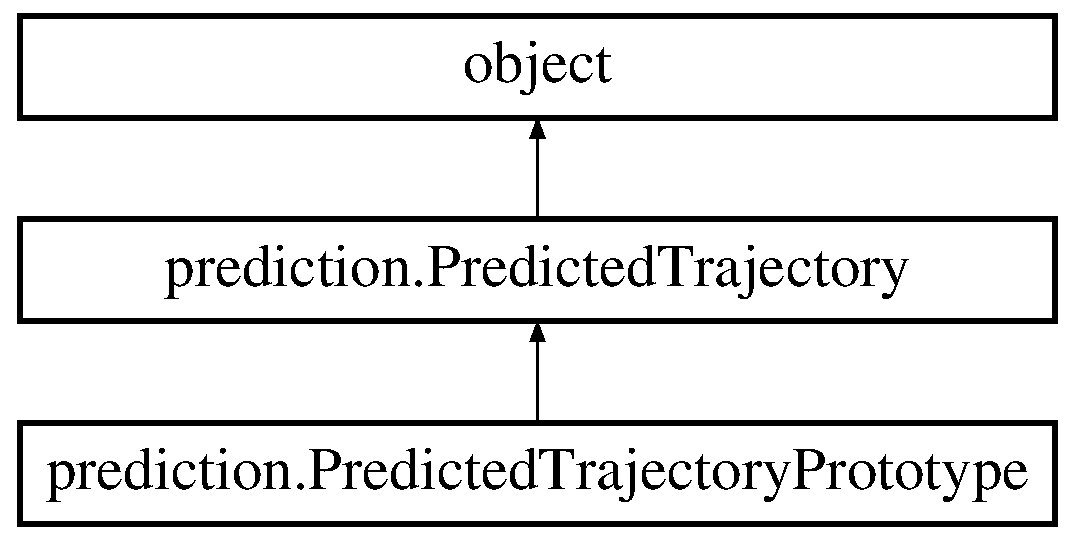
\includegraphics[height=3.000000cm]{classprediction_1_1PredictedTrajectoryPrototype}
\end{center}
\end{figure}
\subsubsection*{Public Member Functions}
\begin{DoxyCompactItemize}
\item 
def \hyperlink{classprediction_1_1PredictedTrajectoryPrototype_ab687233eeac4f24c106086e26b137c94}{\-\_\-\-\_\-init\-\_\-\-\_\-}
\item 
def \hyperlink{classprediction_1_1PredictedTrajectoryPrototype_a0282a109816f59e7548efa08d001d74e}{predict\-Position}
\end{DoxyCompactItemize}
\subsubsection*{Public Attributes}
\begin{DoxyCompactItemize}
\item 
\hyperlink{classprediction_1_1PredictedTrajectoryPrototype_aa7ffee6d30ebbcafe7134c36c6a24d37}{prototype\-Trajectory}
\item 
\hyperlink{classprediction_1_1PredictedTrajectoryPrototype_ac3f37f392469e617f2df0ef190568f9f}{constant\-Speed}
\item 
\hyperlink{classprediction_1_1PredictedTrajectoryPrototype_ae4e01bfd1c77add2c0c7a644f9042fe9}{probability}
\item 
\hyperlink{classprediction_1_1PredictedTrajectoryPrototype_a2626d54e11c5dffd00ea8785c6bb4c81}{predicted\-Positions}
\item 
\hyperlink{classprediction_1_1PredictedTrajectoryPrototype_a57df342a90c6252e7d8f9d986d3001a9}{predicted\-Speed\-Orientations}
\end{DoxyCompactItemize}


\subsubsection{Detailed Description}
\begin{DoxyVerb}Predicted trajectory that follows a prototype trajectory
The prototype is in the format of a moving.Trajectory: it could be
1. an observed trajectory (extracted from video)
2. a generic polyline (eg the road centerline) that a vehicle is supposed to follow

Prediction can be done
1. at constant speed (the instantaneous user speed)
2. following the trajectory path, at the speed of the user
(applying a constant ratio equal 
to the ratio of the user instantaneous speed and the trajectory closest speed)\end{DoxyVerb}
 

\subsubsection{Constructor \& Destructor Documentation}
\hypertarget{classprediction_1_1PredictedTrajectoryPrototype_ab687233eeac4f24c106086e26b137c94}{\index{prediction\-::\-Predicted\-Trajectory\-Prototype@{prediction\-::\-Predicted\-Trajectory\-Prototype}!\-\_\-\-\_\-init\-\_\-\-\_\-@{\-\_\-\-\_\-init\-\_\-\-\_\-}}
\index{\-\_\-\-\_\-init\-\_\-\-\_\-@{\-\_\-\-\_\-init\-\_\-\-\_\-}!prediction::PredictedTrajectoryPrototype@{prediction\-::\-Predicted\-Trajectory\-Prototype}}
\paragraph[{\-\_\-\-\_\-init\-\_\-\-\_\-}]{\setlength{\rightskip}{0pt plus 5cm}def prediction.\-Predicted\-Trajectory\-Prototype.\-\_\-\-\_\-init\-\_\-\-\_\- (
\begin{DoxyParamCaption}
\item[{}]{self, }
\item[{}]{initial\-Position, }
\item[{}]{initial\-Velocity, }
\item[{}]{prototype\-Trajectory, }
\item[{}]{constant\-Speed = {\ttfamily True}, }
\item[{}]{probability = {\ttfamily 1.}}
\end{DoxyParamCaption}
)}}\label{classprediction_1_1PredictedTrajectoryPrototype_ab687233eeac4f24c106086e26b137c94}


\subsubsection{Member Function Documentation}
\hypertarget{classprediction_1_1PredictedTrajectoryPrototype_a0282a109816f59e7548efa08d001d74e}{\index{prediction\-::\-Predicted\-Trajectory\-Prototype@{prediction\-::\-Predicted\-Trajectory\-Prototype}!predict\-Position@{predict\-Position}}
\index{predict\-Position@{predict\-Position}!prediction::PredictedTrajectoryPrototype@{prediction\-::\-Predicted\-Trajectory\-Prototype}}
\paragraph[{predict\-Position}]{\setlength{\rightskip}{0pt plus 5cm}def prediction.\-Predicted\-Trajectory\-Prototype.\-predict\-Position (
\begin{DoxyParamCaption}
\item[{}]{self, }
\item[{}]{n\-Time\-Steps}
\end{DoxyParamCaption}
)}}\label{classprediction_1_1PredictedTrajectoryPrototype_a0282a109816f59e7548efa08d001d74e}


References prediction.\-Predicted\-Trajectory\-Prototype.\-constant\-Speed, prediction.\-find\-Nearest\-Params(), prediction.\-Predicted\-Trajectory.\-predicted\-Positions, prediction.\-Predicted\-Trajectory.\-predicted\-Speed\-Orientations, moving.\-predict\-Position(), and prediction.\-Predicted\-Trajectory\-Prototype.\-prototype\-Trajectory.



\subsubsection{Member Data Documentation}
\hypertarget{classprediction_1_1PredictedTrajectoryPrototype_ac3f37f392469e617f2df0ef190568f9f}{\index{prediction\-::\-Predicted\-Trajectory\-Prototype@{prediction\-::\-Predicted\-Trajectory\-Prototype}!constant\-Speed@{constant\-Speed}}
\index{constant\-Speed@{constant\-Speed}!prediction::PredictedTrajectoryPrototype@{prediction\-::\-Predicted\-Trajectory\-Prototype}}
\paragraph[{constant\-Speed}]{\setlength{\rightskip}{0pt plus 5cm}prediction.\-Predicted\-Trajectory\-Prototype.\-constant\-Speed}}\label{classprediction_1_1PredictedTrajectoryPrototype_ac3f37f392469e617f2df0ef190568f9f}
\hypertarget{classprediction_1_1PredictedTrajectoryPrototype_a2626d54e11c5dffd00ea8785c6bb4c81}{\index{prediction\-::\-Predicted\-Trajectory\-Prototype@{prediction\-::\-Predicted\-Trajectory\-Prototype}!predicted\-Positions@{predicted\-Positions}}
\index{predicted\-Positions@{predicted\-Positions}!prediction::PredictedTrajectoryPrototype@{prediction\-::\-Predicted\-Trajectory\-Prototype}}
\paragraph[{predicted\-Positions}]{\setlength{\rightskip}{0pt plus 5cm}prediction.\-Predicted\-Trajectory\-Prototype.\-predicted\-Positions}}\label{classprediction_1_1PredictedTrajectoryPrototype_a2626d54e11c5dffd00ea8785c6bb4c81}
\hypertarget{classprediction_1_1PredictedTrajectoryPrototype_a57df342a90c6252e7d8f9d986d3001a9}{\index{prediction\-::\-Predicted\-Trajectory\-Prototype@{prediction\-::\-Predicted\-Trajectory\-Prototype}!predicted\-Speed\-Orientations@{predicted\-Speed\-Orientations}}
\index{predicted\-Speed\-Orientations@{predicted\-Speed\-Orientations}!prediction::PredictedTrajectoryPrototype@{prediction\-::\-Predicted\-Trajectory\-Prototype}}
\paragraph[{predicted\-Speed\-Orientations}]{\setlength{\rightskip}{0pt plus 5cm}prediction.\-Predicted\-Trajectory\-Prototype.\-predicted\-Speed\-Orientations}}\label{classprediction_1_1PredictedTrajectoryPrototype_a57df342a90c6252e7d8f9d986d3001a9}
\hypertarget{classprediction_1_1PredictedTrajectoryPrototype_ae4e01bfd1c77add2c0c7a644f9042fe9}{\index{prediction\-::\-Predicted\-Trajectory\-Prototype@{prediction\-::\-Predicted\-Trajectory\-Prototype}!probability@{probability}}
\index{probability@{probability}!prediction::PredictedTrajectoryPrototype@{prediction\-::\-Predicted\-Trajectory\-Prototype}}
\paragraph[{probability}]{\setlength{\rightskip}{0pt plus 5cm}prediction.\-Predicted\-Trajectory\-Prototype.\-probability}}\label{classprediction_1_1PredictedTrajectoryPrototype_ae4e01bfd1c77add2c0c7a644f9042fe9}
\hypertarget{classprediction_1_1PredictedTrajectoryPrototype_aa7ffee6d30ebbcafe7134c36c6a24d37}{\index{prediction\-::\-Predicted\-Trajectory\-Prototype@{prediction\-::\-Predicted\-Trajectory\-Prototype}!prototype\-Trajectory@{prototype\-Trajectory}}
\index{prototype\-Trajectory@{prototype\-Trajectory}!prediction::PredictedTrajectoryPrototype@{prediction\-::\-Predicted\-Trajectory\-Prototype}}
\paragraph[{prototype\-Trajectory}]{\setlength{\rightskip}{0pt plus 5cm}prediction.\-Predicted\-Trajectory\-Prototype.\-prototype\-Trajectory}}\label{classprediction_1_1PredictedTrajectoryPrototype_aa7ffee6d30ebbcafe7134c36c6a24d37}


The documentation for this class was generated from the following file\-:\begin{DoxyCompactItemize}
\item 
python/\hyperlink{prediction_8py}{prediction.\-py}\end{DoxyCompactItemize}

\hypertarget{classprediction_1_1PredictedTrajectoryRandomControl}{\subsection{prediction.\-Predicted\-Trajectory\-Random\-Control Class Reference}
\label{classprediction_1_1PredictedTrajectoryRandomControl}\index{prediction.\-Predicted\-Trajectory\-Random\-Control@{prediction.\-Predicted\-Trajectory\-Random\-Control}}
}
Inheritance diagram for prediction.\-Predicted\-Trajectory\-Random\-Control\-:\begin{figure}[H]
\begin{center}
\leavevmode
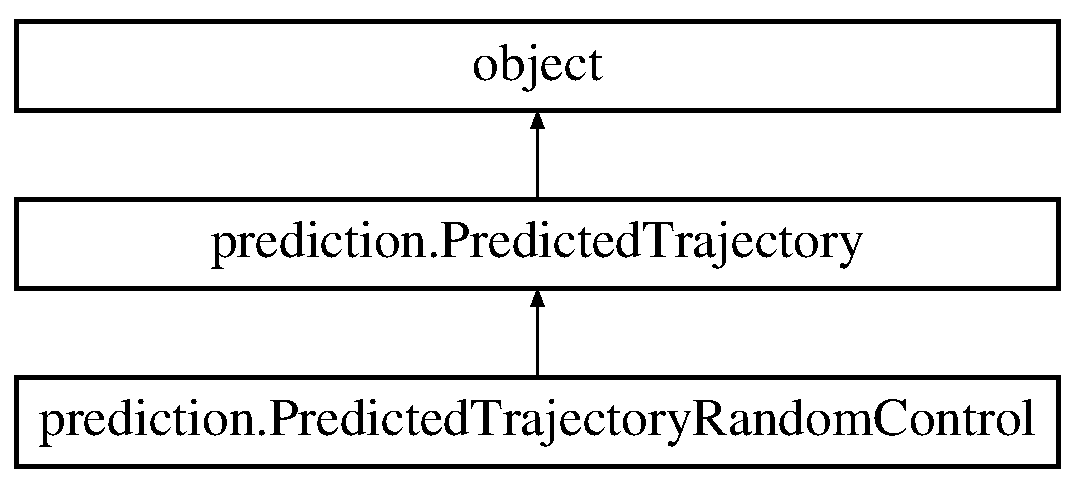
\includegraphics[height=3.000000cm]{classprediction_1_1PredictedTrajectoryRandomControl}
\end{center}
\end{figure}
\subsubsection*{Public Member Functions}
\begin{DoxyCompactItemize}
\item 
def \hyperlink{classprediction_1_1PredictedTrajectoryRandomControl_ab4654da0ee7d4a69dc840edb270c01d2}{\-\_\-\-\_\-init\-\_\-\-\_\-}
\item 
def \hyperlink{classprediction_1_1PredictedTrajectoryRandomControl_a51c585036b06659446c6fcb1e7c38d5e}{get\-Control}
\end{DoxyCompactItemize}
\subsubsection*{Public Attributes}
\begin{DoxyCompactItemize}
\item 
\hyperlink{classprediction_1_1PredictedTrajectoryRandomControl_a37965e61f6213fcff42144a466e15232}{acceleration\-Distribution}
\item 
\hyperlink{classprediction_1_1PredictedTrajectoryRandomControl_a48a17f8abdffcde24cf25b90ebeaf59d}{steering\-Distribution}
\item 
\hyperlink{classprediction_1_1PredictedTrajectoryRandomControl_afb0db36b133a6f189557d35904b49dc2}{max\-Speed}
\item 
\hyperlink{classprediction_1_1PredictedTrajectoryRandomControl_aadf38083f042ae0b97de23c78375eddf}{probability}
\item 
\hyperlink{classprediction_1_1PredictedTrajectoryRandomControl_a1b05261a0f5a1525512441eec9b9e12c}{predicted\-Positions}
\item 
\hyperlink{classprediction_1_1PredictedTrajectoryRandomControl_a7039d42cb1c2150efb1fd21f245f1c51}{predicted\-Speed\-Orientations}
\end{DoxyCompactItemize}


\subsubsection{Detailed Description}
\begin{DoxyVerb}Random vehicle control: suitable for normal adaptation\end{DoxyVerb}
 

\subsubsection{Constructor \& Destructor Documentation}
\hypertarget{classprediction_1_1PredictedTrajectoryRandomControl_ab4654da0ee7d4a69dc840edb270c01d2}{\index{prediction\-::\-Predicted\-Trajectory\-Random\-Control@{prediction\-::\-Predicted\-Trajectory\-Random\-Control}!\-\_\-\-\_\-init\-\_\-\-\_\-@{\-\_\-\-\_\-init\-\_\-\-\_\-}}
\index{\-\_\-\-\_\-init\-\_\-\-\_\-@{\-\_\-\-\_\-init\-\_\-\-\_\-}!prediction::PredictedTrajectoryRandomControl@{prediction\-::\-Predicted\-Trajectory\-Random\-Control}}
\paragraph[{\-\_\-\-\_\-init\-\_\-\-\_\-}]{\setlength{\rightskip}{0pt plus 5cm}def prediction.\-Predicted\-Trajectory\-Random\-Control.\-\_\-\-\_\-init\-\_\-\-\_\- (
\begin{DoxyParamCaption}
\item[{}]{self, }
\item[{}]{initial\-Position, }
\item[{}]{initial\-Velocity, }
\item[{}]{acceleration\-Distribution, }
\item[{}]{steering\-Distribution, }
\item[{}]{probability = {\ttfamily 1.}, }
\item[{}]{max\-Speed = {\ttfamily None}}
\end{DoxyParamCaption}
)}}\label{classprediction_1_1PredictedTrajectoryRandomControl_ab4654da0ee7d4a69dc840edb270c01d2}
\begin{DoxyVerb}Constructor
accelerationDistribution and steeringDistribution are distributions 
that return random numbers drawn from them\end{DoxyVerb}
 

\subsubsection{Member Function Documentation}
\hypertarget{classprediction_1_1PredictedTrajectoryRandomControl_a51c585036b06659446c6fcb1e7c38d5e}{\index{prediction\-::\-Predicted\-Trajectory\-Random\-Control@{prediction\-::\-Predicted\-Trajectory\-Random\-Control}!get\-Control@{get\-Control}}
\index{get\-Control@{get\-Control}!prediction::PredictedTrajectoryRandomControl@{prediction\-::\-Predicted\-Trajectory\-Random\-Control}}
\paragraph[{get\-Control}]{\setlength{\rightskip}{0pt plus 5cm}def prediction.\-Predicted\-Trajectory\-Random\-Control.\-get\-Control (
\begin{DoxyParamCaption}
\item[{}]{self}
\end{DoxyParamCaption}
)}}\label{classprediction_1_1PredictedTrajectoryRandomControl_a51c585036b06659446c6fcb1e7c38d5e}


References prediction.\-Predicted\-Trajectory\-Random\-Control.\-acceleration\-Distribution, and prediction.\-Predicted\-Trajectory\-Random\-Control.\-steering\-Distribution.



\subsubsection{Member Data Documentation}
\hypertarget{classprediction_1_1PredictedTrajectoryRandomControl_a37965e61f6213fcff42144a466e15232}{\index{prediction\-::\-Predicted\-Trajectory\-Random\-Control@{prediction\-::\-Predicted\-Trajectory\-Random\-Control}!acceleration\-Distribution@{acceleration\-Distribution}}
\index{acceleration\-Distribution@{acceleration\-Distribution}!prediction::PredictedTrajectoryRandomControl@{prediction\-::\-Predicted\-Trajectory\-Random\-Control}}
\paragraph[{acceleration\-Distribution}]{\setlength{\rightskip}{0pt plus 5cm}prediction.\-Predicted\-Trajectory\-Random\-Control.\-acceleration\-Distribution}}\label{classprediction_1_1PredictedTrajectoryRandomControl_a37965e61f6213fcff42144a466e15232}
\hypertarget{classprediction_1_1PredictedTrajectoryRandomControl_afb0db36b133a6f189557d35904b49dc2}{\index{prediction\-::\-Predicted\-Trajectory\-Random\-Control@{prediction\-::\-Predicted\-Trajectory\-Random\-Control}!max\-Speed@{max\-Speed}}
\index{max\-Speed@{max\-Speed}!prediction::PredictedTrajectoryRandomControl@{prediction\-::\-Predicted\-Trajectory\-Random\-Control}}
\paragraph[{max\-Speed}]{\setlength{\rightskip}{0pt plus 5cm}prediction.\-Predicted\-Trajectory\-Random\-Control.\-max\-Speed}}\label{classprediction_1_1PredictedTrajectoryRandomControl_afb0db36b133a6f189557d35904b49dc2}
\hypertarget{classprediction_1_1PredictedTrajectoryRandomControl_a1b05261a0f5a1525512441eec9b9e12c}{\index{prediction\-::\-Predicted\-Trajectory\-Random\-Control@{prediction\-::\-Predicted\-Trajectory\-Random\-Control}!predicted\-Positions@{predicted\-Positions}}
\index{predicted\-Positions@{predicted\-Positions}!prediction::PredictedTrajectoryRandomControl@{prediction\-::\-Predicted\-Trajectory\-Random\-Control}}
\paragraph[{predicted\-Positions}]{\setlength{\rightskip}{0pt plus 5cm}prediction.\-Predicted\-Trajectory\-Random\-Control.\-predicted\-Positions}}\label{classprediction_1_1PredictedTrajectoryRandomControl_a1b05261a0f5a1525512441eec9b9e12c}
\hypertarget{classprediction_1_1PredictedTrajectoryRandomControl_a7039d42cb1c2150efb1fd21f245f1c51}{\index{prediction\-::\-Predicted\-Trajectory\-Random\-Control@{prediction\-::\-Predicted\-Trajectory\-Random\-Control}!predicted\-Speed\-Orientations@{predicted\-Speed\-Orientations}}
\index{predicted\-Speed\-Orientations@{predicted\-Speed\-Orientations}!prediction::PredictedTrajectoryRandomControl@{prediction\-::\-Predicted\-Trajectory\-Random\-Control}}
\paragraph[{predicted\-Speed\-Orientations}]{\setlength{\rightskip}{0pt plus 5cm}prediction.\-Predicted\-Trajectory\-Random\-Control.\-predicted\-Speed\-Orientations}}\label{classprediction_1_1PredictedTrajectoryRandomControl_a7039d42cb1c2150efb1fd21f245f1c51}
\hypertarget{classprediction_1_1PredictedTrajectoryRandomControl_aadf38083f042ae0b97de23c78375eddf}{\index{prediction\-::\-Predicted\-Trajectory\-Random\-Control@{prediction\-::\-Predicted\-Trajectory\-Random\-Control}!probability@{probability}}
\index{probability@{probability}!prediction::PredictedTrajectoryRandomControl@{prediction\-::\-Predicted\-Trajectory\-Random\-Control}}
\paragraph[{probability}]{\setlength{\rightskip}{0pt plus 5cm}prediction.\-Predicted\-Trajectory\-Random\-Control.\-probability}}\label{classprediction_1_1PredictedTrajectoryRandomControl_aadf38083f042ae0b97de23c78375eddf}
\hypertarget{classprediction_1_1PredictedTrajectoryRandomControl_a48a17f8abdffcde24cf25b90ebeaf59d}{\index{prediction\-::\-Predicted\-Trajectory\-Random\-Control@{prediction\-::\-Predicted\-Trajectory\-Random\-Control}!steering\-Distribution@{steering\-Distribution}}
\index{steering\-Distribution@{steering\-Distribution}!prediction::PredictedTrajectoryRandomControl@{prediction\-::\-Predicted\-Trajectory\-Random\-Control}}
\paragraph[{steering\-Distribution}]{\setlength{\rightskip}{0pt plus 5cm}prediction.\-Predicted\-Trajectory\-Random\-Control.\-steering\-Distribution}}\label{classprediction_1_1PredictedTrajectoryRandomControl_a48a17f8abdffcde24cf25b90ebeaf59d}


The documentation for this class was generated from the following file\-:\begin{DoxyCompactItemize}
\item 
python/\hyperlink{prediction_8py}{prediction.\-py}\end{DoxyCompactItemize}

\hypertarget{classprediction_1_1PredictionParameters}{\subsection{prediction.\-Prediction\-Parameters Class Reference}
\label{classprediction_1_1PredictionParameters}\index{prediction.\-Prediction\-Parameters@{prediction.\-Prediction\-Parameters}}
}
Inheritance diagram for prediction.\-Prediction\-Parameters\-:\begin{figure}[H]
\begin{center}
\leavevmode
\includegraphics[height=0.797342cm]{classprediction_1_1PredictionParameters}
\end{center}
\end{figure}
\subsubsection*{Public Member Functions}
\begin{DoxyCompactItemize}
\item 
def \hyperlink{classprediction_1_1PredictionParameters_a2bc846706f44db9aee7be414c7876b0e}{\-\_\-\-\_\-init\-\_\-\-\_\-}
\item 
def \hyperlink{classprediction_1_1PredictionParameters_a8630b919e5af565a1f755e8bc7c97317}{\-\_\-\-\_\-str\-\_\-\-\_\-}
\item 
def \hyperlink{classprediction_1_1PredictionParameters_a2288708cc66b10f251b16e6954f19e86}{generate\-Predicted\-Trajectories}
\item 
def \hyperlink{classprediction_1_1PredictionParameters_ad99f4942743514bad8eb870f95136964}{compute\-Crossings\-Collisions\-At\-Instant}
\item 
def \hyperlink{classprediction_1_1PredictionParameters_abe5a90b1762ee95353b9acbe6f98df9a}{compute\-Crossings\-Collisions}
\item 
def \hyperlink{classprediction_1_1PredictionParameters_add13fc0a539ca2cffaa630e5de421607}{compute\-Collision\-Probability}
\end{DoxyCompactItemize}
\subsubsection*{Public Attributes}
\begin{DoxyCompactItemize}
\item 
\hyperlink{classprediction_1_1PredictionParameters_a801f3373849862455991db0882908ea2}{name}
\item 
\hyperlink{classprediction_1_1PredictionParameters_aecd38f89045d75366021047fb06fe885}{max\-Speed}
\end{DoxyCompactItemize}


\subsubsection{Constructor \& Destructor Documentation}
\hypertarget{classprediction_1_1PredictionParameters_a2bc846706f44db9aee7be414c7876b0e}{\index{prediction\-::\-Prediction\-Parameters@{prediction\-::\-Prediction\-Parameters}!\-\_\-\-\_\-init\-\_\-\-\_\-@{\-\_\-\-\_\-init\-\_\-\-\_\-}}
\index{\-\_\-\-\_\-init\-\_\-\-\_\-@{\-\_\-\-\_\-init\-\_\-\-\_\-}!prediction::PredictionParameters@{prediction\-::\-Prediction\-Parameters}}
\paragraph[{\-\_\-\-\_\-init\-\_\-\-\_\-}]{\setlength{\rightskip}{0pt plus 5cm}def prediction.\-Prediction\-Parameters.\-\_\-\-\_\-init\-\_\-\-\_\- (
\begin{DoxyParamCaption}
\item[{}]{self, }
\item[{}]{name, }
\item[{}]{max\-Speed}
\end{DoxyParamCaption}
)}}\label{classprediction_1_1PredictionParameters_a2bc846706f44db9aee7be414c7876b0e}


\subsubsection{Member Function Documentation}
\hypertarget{classprediction_1_1PredictionParameters_a8630b919e5af565a1f755e8bc7c97317}{\index{prediction\-::\-Prediction\-Parameters@{prediction\-::\-Prediction\-Parameters}!\-\_\-\-\_\-str\-\_\-\-\_\-@{\-\_\-\-\_\-str\-\_\-\-\_\-}}
\index{\-\_\-\-\_\-str\-\_\-\-\_\-@{\-\_\-\-\_\-str\-\_\-\-\_\-}!prediction::PredictionParameters@{prediction\-::\-Prediction\-Parameters}}
\paragraph[{\-\_\-\-\_\-str\-\_\-\-\_\-}]{\setlength{\rightskip}{0pt plus 5cm}def prediction.\-Prediction\-Parameters.\-\_\-\-\_\-str\-\_\-\-\_\- (
\begin{DoxyParamCaption}
\item[{}]{self}
\end{DoxyParamCaption}
)}}\label{classprediction_1_1PredictionParameters_a8630b919e5af565a1f755e8bc7c97317}


References prediction.\-Predicted\-Trajectory\-Constant.\-max\-Speed, prediction.\-Predicted\-Trajectory\-Random\-Control.\-max\-Speed, prediction.\-Prediction\-Parameters.\-max\-Speed, metadata.\-Site.\-name, indicators.\-Temporal\-Indicator.\-name, metadata.\-Video\-Sequence.\-name, pavement.\-R\-T\-S\-S.\-name, and prediction.\-Prediction\-Parameters.\-name.

\hypertarget{classprediction_1_1PredictionParameters_add13fc0a539ca2cffaa630e5de421607}{\index{prediction\-::\-Prediction\-Parameters@{prediction\-::\-Prediction\-Parameters}!compute\-Collision\-Probability@{compute\-Collision\-Probability}}
\index{compute\-Collision\-Probability@{compute\-Collision\-Probability}!prediction::PredictionParameters@{prediction\-::\-Prediction\-Parameters}}
\paragraph[{compute\-Collision\-Probability}]{\setlength{\rightskip}{0pt plus 5cm}def prediction.\-Prediction\-Parameters.\-compute\-Collision\-Probability (
\begin{DoxyParamCaption}
\item[{}]{self, }
\item[{}]{obj1, }
\item[{}]{obj2, }
\item[{}]{collision\-Distance\-Threshold, }
\item[{}]{time\-Horizon, }
\item[{}]{debug = {\ttfamily False}, }
\item[{}]{time\-Interval = {\ttfamily None}}
\end{DoxyParamCaption}
)}}\label{classprediction_1_1PredictionParameters_add13fc0a539ca2cffaa630e5de421607}
\begin{DoxyVerb}Computes only collision probabilities
Returns for each instant the collision probability and number of samples drawn\end{DoxyVerb}
 

References prediction.\-compute\-Collision\-Time(), prediction.\-Prediction\-Parameters.\-generate\-Predicted\-Trajectories(), and prediction.\-save\-Predicted\-Trajectories\-Figure().

\hypertarget{classprediction_1_1PredictionParameters_abe5a90b1762ee95353b9acbe6f98df9a}{\index{prediction\-::\-Prediction\-Parameters@{prediction\-::\-Prediction\-Parameters}!compute\-Crossings\-Collisions@{compute\-Crossings\-Collisions}}
\index{compute\-Crossings\-Collisions@{compute\-Crossings\-Collisions}!prediction::PredictionParameters@{prediction\-::\-Prediction\-Parameters}}
\paragraph[{compute\-Crossings\-Collisions}]{\setlength{\rightskip}{0pt plus 5cm}def prediction.\-Prediction\-Parameters.\-compute\-Crossings\-Collisions (
\begin{DoxyParamCaption}
\item[{}]{self, }
\item[{}]{obj1, }
\item[{}]{obj2, }
\item[{}]{collision\-Distance\-Threshold, }
\item[{}]{time\-Horizon, }
\item[{}]{compute\-C\-Z = {\ttfamily False}, }
\item[{}]{debug = {\ttfamily False}, }
\item[{}]{time\-Interval = {\ttfamily None}, }
\item[{}]{n\-Processes = {\ttfamily 1}, }
\item[{}]{use\-Prototypes = {\ttfamily False}, }
\item[{}]{route1 = {\ttfamily (-\/1,-\/1}, }
\item[{}]{route2 = {\ttfamily (-\/1,-\/1}, }
\item[{}]{prototypes = {\ttfamily \{\}}, }
\item[{}]{second\-Step\-Prototypes = {\ttfamily \{\}}, }
\item[{}]{n\-Matching = {\ttfamily \{\}}, }
\item[{}]{objects = {\ttfamily \mbox{[}\mbox{]}}, }
\item[{}]{noise\-Entry\-Nums = {\ttfamily \mbox{[}\mbox{]}}, }
\item[{}]{noise\-Exit\-Nums = {\ttfamily \mbox{[}\mbox{]}}, }
\item[{}]{min\-Similarity = {\ttfamily 0.1}, }
\item[{}]{most\-Matched = {\ttfamily None}, }
\item[{}]{use\-Destination = {\ttfamily True}, }
\item[{}]{use\-Speed\-Prototype = {\ttfamily True}, }
\item[{}]{accept\-Partial\-Length = {\ttfamily 30}, }
\item[{}]{step = {\ttfamily 1}}
\end{DoxyParamCaption}
)}}\label{classprediction_1_1PredictionParameters_abe5a90b1762ee95353b9acbe6f98df9a}
\begin{DoxyVerb}Computes all crossing and collision points at each common instant for two road users. \end{DoxyVerb}
 

References prediction.\-Prediction\-Parameters.\-compute\-Crossings\-Collisions\-At\-Instant().

\hypertarget{classprediction_1_1PredictionParameters_ad99f4942743514bad8eb870f95136964}{\index{prediction\-::\-Prediction\-Parameters@{prediction\-::\-Prediction\-Parameters}!compute\-Crossings\-Collisions\-At\-Instant@{compute\-Crossings\-Collisions\-At\-Instant}}
\index{compute\-Crossings\-Collisions\-At\-Instant@{compute\-Crossings\-Collisions\-At\-Instant}!prediction::PredictionParameters@{prediction\-::\-Prediction\-Parameters}}
\paragraph[{compute\-Crossings\-Collisions\-At\-Instant}]{\setlength{\rightskip}{0pt plus 5cm}def prediction.\-Prediction\-Parameters.\-compute\-Crossings\-Collisions\-At\-Instant (
\begin{DoxyParamCaption}
\item[{}]{self, }
\item[{}]{current\-Instant, }
\item[{}]{obj1, }
\item[{}]{obj2, }
\item[{}]{collision\-Distance\-Threshold, }
\item[{}]{time\-Horizon, }
\item[{}]{compute\-C\-Z = {\ttfamily False}, }
\item[{}]{debug = {\ttfamily False}, }
\item[{}]{use\-Prototypes = {\ttfamily False}, }
\item[{}]{route1 = {\ttfamily (-\/1,-\/1}, }
\item[{}]{route2 = {\ttfamily (-\/1,-\/1}, }
\item[{}]{prototypes = {\ttfamily \{\}}, }
\item[{}]{second\-Step\-Prototypes = {\ttfamily \{\}}, }
\item[{}]{n\-Matching = {\ttfamily \{\}}, }
\item[{}]{objects = {\ttfamily \mbox{[}\mbox{]}}, }
\item[{}]{noise\-Entry\-Nums = {\ttfamily \mbox{[}\mbox{]}}, }
\item[{}]{noise\-Exit\-Nums = {\ttfamily \mbox{[}\mbox{]}}, }
\item[{}]{min\-Similarity = {\ttfamily 0.1}, }
\item[{}]{most\-Matched = {\ttfamily None}, }
\item[{}]{use\-Destination = {\ttfamily True}, }
\item[{}]{use\-Speed\-Prototype = {\ttfamily True}}
\end{DoxyParamCaption}
)}}\label{classprediction_1_1PredictionParameters_ad99f4942743514bad8eb870f95136964}
\hypertarget{classprediction_1_1PredictionParameters_a2288708cc66b10f251b16e6954f19e86}{\index{prediction\-::\-Prediction\-Parameters@{prediction\-::\-Prediction\-Parameters}!generate\-Predicted\-Trajectories@{generate\-Predicted\-Trajectories}}
\index{generate\-Predicted\-Trajectories@{generate\-Predicted\-Trajectories}!prediction::PredictionParameters@{prediction\-::\-Prediction\-Parameters}}
\paragraph[{generate\-Predicted\-Trajectories}]{\setlength{\rightskip}{0pt plus 5cm}def prediction.\-Prediction\-Parameters.\-generate\-Predicted\-Trajectories (
\begin{DoxyParamCaption}
\item[{}]{self, }
\item[{}]{obj, }
\item[{}]{instant}
\end{DoxyParamCaption}
)}}\label{classprediction_1_1PredictionParameters_a2288708cc66b10f251b16e6954f19e86}


\subsubsection{Member Data Documentation}
\hypertarget{classprediction_1_1PredictionParameters_aecd38f89045d75366021047fb06fe885}{\index{prediction\-::\-Prediction\-Parameters@{prediction\-::\-Prediction\-Parameters}!max\-Speed@{max\-Speed}}
\index{max\-Speed@{max\-Speed}!prediction::PredictionParameters@{prediction\-::\-Prediction\-Parameters}}
\paragraph[{max\-Speed}]{\setlength{\rightskip}{0pt plus 5cm}prediction.\-Prediction\-Parameters.\-max\-Speed}}\label{classprediction_1_1PredictionParameters_aecd38f89045d75366021047fb06fe885}
\hypertarget{classprediction_1_1PredictionParameters_a801f3373849862455991db0882908ea2}{\index{prediction\-::\-Prediction\-Parameters@{prediction\-::\-Prediction\-Parameters}!name@{name}}
\index{name@{name}!prediction::PredictionParameters@{prediction\-::\-Prediction\-Parameters}}
\paragraph[{name}]{\setlength{\rightskip}{0pt plus 5cm}prediction.\-Prediction\-Parameters.\-name}}\label{classprediction_1_1PredictionParameters_a801f3373849862455991db0882908ea2}


The documentation for this class was generated from the following file\-:\begin{DoxyCompactItemize}
\item 
python/\hyperlink{prediction_8py}{prediction.\-py}\end{DoxyCompactItemize}

\hypertarget{classstorage_1_1ProcessParameters}{\subsection{storage.\-Process\-Parameters Class Reference}
\label{classstorage_1_1ProcessParameters}\index{storage.\-Process\-Parameters@{storage.\-Process\-Parameters}}
}


Utils to read .ini type text files for configuration, meta data...  


Inheritance diagram for storage.\-Process\-Parameters\-:\begin{figure}[H]
\begin{center}
\leavevmode
\includegraphics[height=3.000000cm]{classstorage_1_1ProcessParameters}
\end{center}
\end{figure}
\subsubsection*{Public Member Functions}
\begin{DoxyCompactItemize}
\item 
def \hyperlink{classstorage_1_1ProcessParameters_ae5638fb6be16b5c2a02311817d8a1362}{load\-Config\-File}
\item 
def \hyperlink{classstorage_1_1ProcessParameters_a3a5510c748699d3247288e473ee844b8}{\-\_\-\-\_\-init\-\_\-\-\_\-}
\item 
def \hyperlink{classstorage_1_1ProcessParameters_a48ee592e21e7aec5028d192085c59010}{convert\-To\-Frames}
\end{DoxyCompactItemize}
\subsubsection*{Public Attributes}
\begin{DoxyCompactItemize}
\item 
\hyperlink{classstorage_1_1ProcessParameters_a8d06979c0292afa30e5b9a0cd7da1367}{section\-Header}
\item 
\hyperlink{classstorage_1_1ProcessParameters_a7d08be6d2b8023fe12aaf0f5fa1ee335}{video\-Filename}
\item 
\hyperlink{classstorage_1_1ProcessParameters_a4611b5effbff8949a3498861ba92d5d5}{database\-Filename}
\item 
\hyperlink{classstorage_1_1ProcessParameters_aed88a4aec4b3f18b05316952da6993e4}{homography\-Filename}
\item 
\hyperlink{classstorage_1_1ProcessParameters_a5c1647945769d794f0335e119d09ad1d}{homography}
\item 
\hyperlink{classstorage_1_1ProcessParameters_a3b9f0776b81d334f25d705bdb4c77e68}{intrinsic\-Camera\-Filename}
\item 
\hyperlink{classstorage_1_1ProcessParameters_a14422d1518a71a079c64938a59ff36d0}{intrinsic\-Camera\-Matrix}
\item 
\hyperlink{classstorage_1_1ProcessParameters_aa1a5dfd672fb3f66b7bcdc973350a580}{distortion\-Coefficients}
\item 
\hyperlink{classstorage_1_1ProcessParameters_add290dd3a09688dc0b2587f99f8c0d10}{undistorted\-Image\-Multiplication}
\item 
\hyperlink{classstorage_1_1ProcessParameters_a0b0facdf5f480b87c24a1b97381bdaad}{undistort}
\item 
\hyperlink{classstorage_1_1ProcessParameters_ac4393b9ae6e8b573ef292dc9ebadece7}{first\-Frame\-Num}
\item 
\hyperlink{classstorage_1_1ProcessParameters_ae3cd89ca34997fb567ff5c6ecebc855f}{video\-Frame\-Rate}
\item 
\hyperlink{classstorage_1_1ProcessParameters_a3a493868a73793b001c233770cc1e813}{speed\-Aggregation\-Method}
\item 
\hyperlink{classstorage_1_1ProcessParameters_a3cfd04661ca88760f29f88328bebab1c}{n\-Frames\-Ignore\-At\-Ends}
\item 
\hyperlink{classstorage_1_1ProcessParameters_a3a89cfa1826ee1b2758b01bb16ad9ea9}{speed\-Aggregation\-Quantile}
\item 
\hyperlink{classstorage_1_1ProcessParameters_a263ea38ba109d9b0684328c7d709e439}{min\-Speed\-Equiprobable}
\item 
\hyperlink{classstorage_1_1ProcessParameters_a52d5bcaaca46f651fc56468d8392304e}{min\-N\-Pixels}
\item 
\hyperlink{classstorage_1_1ProcessParameters_aaf6c2c561a0d3d236d0eb63373cd1a6e}{ped\-Bike\-Car\-S\-V\-M\-Filename}
\item 
\hyperlink{classstorage_1_1ProcessParameters_aba0567cbcab31cdb6ca4625561663d0d}{bike\-Car\-S\-V\-M\-Filename}
\item 
\hyperlink{classstorage_1_1ProcessParameters_a56e661759fd66c15547cd998172c96db}{max\-Pedestrian\-Speed}
\item 
\hyperlink{classstorage_1_1ProcessParameters_a3d8a7116c15a02d9db445bf6a3d8f810}{max\-Cyclist\-Speed}
\item 
\hyperlink{classstorage_1_1ProcessParameters_a7307011b1a2a1fcb77c11c0f6e056a50}{mean\-Pedestrian\-Speed}
\item 
\hyperlink{classstorage_1_1ProcessParameters_a1fcc179ff1fffefd797ab8298015af6d}{std\-Pedestrian\-Speed}
\item 
\hyperlink{classstorage_1_1ProcessParameters_a9b1b8e777ddee3283200daee124c2b0a}{location\-Cyclist\-Speed}
\item 
\hyperlink{classstorage_1_1ProcessParameters_a0ca83a34492b39e327b7823f1e047b03}{scale\-Cyclist\-Speed}
\item 
\hyperlink{classstorage_1_1ProcessParameters_a3dd26255d164503bdee5a4065a907c45}{mean\-Vehicle\-Speed}
\item 
\hyperlink{classstorage_1_1ProcessParameters_a52665332feb3d34a1466c834156e33fa}{std\-Vehicle\-Speed}
\item 
\hyperlink{classstorage_1_1ProcessParameters_acd7135dcbc9de062b30c18eb3f4b52b4}{max\-Predicted\-Speed}
\item 
\hyperlink{classstorage_1_1ProcessParameters_a90c11b4df9e54ffec746cd31bdf3a78c}{prediction\-Time\-Horizon}
\item 
\hyperlink{classstorage_1_1ProcessParameters_aa3d2c35d0892ac429ca3c2db6be63f0b}{collision\-Distance}
\item 
\hyperlink{classstorage_1_1ProcessParameters_a30113766c8b8b7aae3901eebde57ddeb}{crossing\-Zones}
\item 
\hyperlink{classstorage_1_1ProcessParameters_af2c45d64e2262e770e2618c516e068e7}{prediction\-Method}
\item 
\hyperlink{classstorage_1_1ProcessParameters_a4353287483a57a4554376f7a9d27203e}{n\-Predicted\-Trajectories}
\item 
\hyperlink{classstorage_1_1ProcessParameters_a444e623a716d254348c5801f635b2d11}{max\-Normal\-Acceleration}
\item 
\hyperlink{classstorage_1_1ProcessParameters_ac16c180166a37493f96704e46ec762b0}{max\-Normal\-Steering}
\item 
\hyperlink{classstorage_1_1ProcessParameters_a880b57c442c629b5cdb539ef782a241d}{min\-Extreme\-Acceleration}
\item 
\hyperlink{classstorage_1_1ProcessParameters_a491518de08a7a5bf370c180537f1d2cd}{max\-Extreme\-Acceleration}
\item 
\hyperlink{classstorage_1_1ProcessParameters_a48e98493c201383a69dbeef05592ba3b}{max\-Extreme\-Steering}
\item 
\hyperlink{classstorage_1_1ProcessParameters_a62a5c6745fea27b265ba00b03c4204dd}{use\-Features\-For\-Prediction}
\end{DoxyCompactItemize}


\subsubsection{Detailed Description}
Utils to read .ini type text files for configuration, meta data... 

\begin{DoxyVerb}Class for all parameters controlling data processing: input,
method parameters, etc. for tracking, classification and safety

Note: framerate is already taken into account\end{DoxyVerb}
 

\subsubsection{Constructor \& Destructor Documentation}
\hypertarget{classstorage_1_1ProcessParameters_a3a5510c748699d3247288e473ee844b8}{\index{storage\-::\-Process\-Parameters@{storage\-::\-Process\-Parameters}!\-\_\-\-\_\-init\-\_\-\-\_\-@{\-\_\-\-\_\-init\-\_\-\-\_\-}}
\index{\-\_\-\-\_\-init\-\_\-\-\_\-@{\-\_\-\-\_\-init\-\_\-\-\_\-}!storage::ProcessParameters@{storage\-::\-Process\-Parameters}}
\paragraph[{\-\_\-\-\_\-init\-\_\-\-\_\-}]{\setlength{\rightskip}{0pt plus 5cm}def storage.\-Process\-Parameters.\-\_\-\-\_\-init\-\_\-\-\_\- (
\begin{DoxyParamCaption}
\item[{}]{self, }
\item[{}]{filename = {\ttfamily None}}
\end{DoxyParamCaption}
)}}\label{classstorage_1_1ProcessParameters_a3a5510c748699d3247288e473ee844b8}


References storage.\-Process\-Parameters.\-load\-Config\-File().



\subsubsection{Member Function Documentation}
\hypertarget{classstorage_1_1ProcessParameters_a48ee592e21e7aec5028d192085c59010}{\index{storage\-::\-Process\-Parameters@{storage\-::\-Process\-Parameters}!convert\-To\-Frames@{convert\-To\-Frames}}
\index{convert\-To\-Frames@{convert\-To\-Frames}!storage::ProcessParameters@{storage\-::\-Process\-Parameters}}
\paragraph[{convert\-To\-Frames}]{\setlength{\rightskip}{0pt plus 5cm}def storage.\-Process\-Parameters.\-convert\-To\-Frames (
\begin{DoxyParamCaption}
\item[{}]{self, }
\item[{}]{speed\-Ratio = {\ttfamily 3.6}}
\end{DoxyParamCaption}
)}}\label{classstorage_1_1ProcessParameters_a48ee592e21e7aec5028d192085c59010}
\begin{DoxyVerb}Converts parameters with a relationship to time in 'native' frame time
speedRatio is the conversion from the speed unit in the config file
to the distance per second

ie param(config file) = speedRatio x fps x param(used in program)
eg km/h = 3.6 (m/s to km/h) x frame/s x m/frame\end{DoxyVerb}
 

References storage.\-Process\-Parameters.\-location\-Cyclist\-Speed, storage.\-Process\-Parameters.\-max\-Cyclist\-Speed, storage.\-Process\-Parameters.\-max\-Pedestrian\-Speed, storage.\-Process\-Parameters.\-mean\-Pedestrian\-Speed, storage.\-Process\-Parameters.\-mean\-Vehicle\-Speed, storage.\-Process\-Parameters.\-min\-Speed\-Equiprobable, storage.\-Process\-Parameters.\-std\-Pedestrian\-Speed, storage.\-Process\-Parameters.\-std\-Vehicle\-Speed, and storage.\-Process\-Parameters.\-video\-Frame\-Rate.

\hypertarget{classstorage_1_1ProcessParameters_ae5638fb6be16b5c2a02311817d8a1362}{\index{storage\-::\-Process\-Parameters@{storage\-::\-Process\-Parameters}!load\-Config\-File@{load\-Config\-File}}
\index{load\-Config\-File@{load\-Config\-File}!storage::ProcessParameters@{storage\-::\-Process\-Parameters}}
\paragraph[{load\-Config\-File}]{\setlength{\rightskip}{0pt plus 5cm}def storage.\-Process\-Parameters.\-load\-Config\-File (
\begin{DoxyParamCaption}
\item[{}]{self, }
\item[{}]{filename}
\end{DoxyParamCaption}
)}}\label{classstorage_1_1ProcessParameters_ae5638fb6be16b5c2a02311817d8a1362}


References storage.\-open\-Check().



\subsubsection{Member Data Documentation}
\hypertarget{classstorage_1_1ProcessParameters_aba0567cbcab31cdb6ca4625561663d0d}{\index{storage\-::\-Process\-Parameters@{storage\-::\-Process\-Parameters}!bike\-Car\-S\-V\-M\-Filename@{bike\-Car\-S\-V\-M\-Filename}}
\index{bike\-Car\-S\-V\-M\-Filename@{bike\-Car\-S\-V\-M\-Filename}!storage::ProcessParameters@{storage\-::\-Process\-Parameters}}
\paragraph[{bike\-Car\-S\-V\-M\-Filename}]{\setlength{\rightskip}{0pt plus 5cm}storage.\-Process\-Parameters.\-bike\-Car\-S\-V\-M\-Filename}}\label{classstorage_1_1ProcessParameters_aba0567cbcab31cdb6ca4625561663d0d}
\hypertarget{classstorage_1_1ProcessParameters_aa3d2c35d0892ac429ca3c2db6be63f0b}{\index{storage\-::\-Process\-Parameters@{storage\-::\-Process\-Parameters}!collision\-Distance@{collision\-Distance}}
\index{collision\-Distance@{collision\-Distance}!storage::ProcessParameters@{storage\-::\-Process\-Parameters}}
\paragraph[{collision\-Distance}]{\setlength{\rightskip}{0pt plus 5cm}storage.\-Process\-Parameters.\-collision\-Distance}}\label{classstorage_1_1ProcessParameters_aa3d2c35d0892ac429ca3c2db6be63f0b}
\hypertarget{classstorage_1_1ProcessParameters_a30113766c8b8b7aae3901eebde57ddeb}{\index{storage\-::\-Process\-Parameters@{storage\-::\-Process\-Parameters}!crossing\-Zones@{crossing\-Zones}}
\index{crossing\-Zones@{crossing\-Zones}!storage::ProcessParameters@{storage\-::\-Process\-Parameters}}
\paragraph[{crossing\-Zones}]{\setlength{\rightskip}{0pt plus 5cm}storage.\-Process\-Parameters.\-crossing\-Zones}}\label{classstorage_1_1ProcessParameters_a30113766c8b8b7aae3901eebde57ddeb}
\hypertarget{classstorage_1_1ProcessParameters_a4611b5effbff8949a3498861ba92d5d5}{\index{storage\-::\-Process\-Parameters@{storage\-::\-Process\-Parameters}!database\-Filename@{database\-Filename}}
\index{database\-Filename@{database\-Filename}!storage::ProcessParameters@{storage\-::\-Process\-Parameters}}
\paragraph[{database\-Filename}]{\setlength{\rightskip}{0pt plus 5cm}storage.\-Process\-Parameters.\-database\-Filename}}\label{classstorage_1_1ProcessParameters_a4611b5effbff8949a3498861ba92d5d5}
\hypertarget{classstorage_1_1ProcessParameters_aa1a5dfd672fb3f66b7bcdc973350a580}{\index{storage\-::\-Process\-Parameters@{storage\-::\-Process\-Parameters}!distortion\-Coefficients@{distortion\-Coefficients}}
\index{distortion\-Coefficients@{distortion\-Coefficients}!storage::ProcessParameters@{storage\-::\-Process\-Parameters}}
\paragraph[{distortion\-Coefficients}]{\setlength{\rightskip}{0pt plus 5cm}storage.\-Process\-Parameters.\-distortion\-Coefficients}}\label{classstorage_1_1ProcessParameters_aa1a5dfd672fb3f66b7bcdc973350a580}
\hypertarget{classstorage_1_1ProcessParameters_ac4393b9ae6e8b573ef292dc9ebadece7}{\index{storage\-::\-Process\-Parameters@{storage\-::\-Process\-Parameters}!first\-Frame\-Num@{first\-Frame\-Num}}
\index{first\-Frame\-Num@{first\-Frame\-Num}!storage::ProcessParameters@{storage\-::\-Process\-Parameters}}
\paragraph[{first\-Frame\-Num}]{\setlength{\rightskip}{0pt plus 5cm}storage.\-Process\-Parameters.\-first\-Frame\-Num}}\label{classstorage_1_1ProcessParameters_ac4393b9ae6e8b573ef292dc9ebadece7}
\hypertarget{classstorage_1_1ProcessParameters_a5c1647945769d794f0335e119d09ad1d}{\index{storage\-::\-Process\-Parameters@{storage\-::\-Process\-Parameters}!homography@{homography}}
\index{homography@{homography}!storage::ProcessParameters@{storage\-::\-Process\-Parameters}}
\paragraph[{homography}]{\setlength{\rightskip}{0pt plus 5cm}storage.\-Process\-Parameters.\-homography}}\label{classstorage_1_1ProcessParameters_a5c1647945769d794f0335e119d09ad1d}
\hypertarget{classstorage_1_1ProcessParameters_aed88a4aec4b3f18b05316952da6993e4}{\index{storage\-::\-Process\-Parameters@{storage\-::\-Process\-Parameters}!homography\-Filename@{homography\-Filename}}
\index{homography\-Filename@{homography\-Filename}!storage::ProcessParameters@{storage\-::\-Process\-Parameters}}
\paragraph[{homography\-Filename}]{\setlength{\rightskip}{0pt plus 5cm}storage.\-Process\-Parameters.\-homography\-Filename}}\label{classstorage_1_1ProcessParameters_aed88a4aec4b3f18b05316952da6993e4}
\hypertarget{classstorage_1_1ProcessParameters_a3b9f0776b81d334f25d705bdb4c77e68}{\index{storage\-::\-Process\-Parameters@{storage\-::\-Process\-Parameters}!intrinsic\-Camera\-Filename@{intrinsic\-Camera\-Filename}}
\index{intrinsic\-Camera\-Filename@{intrinsic\-Camera\-Filename}!storage::ProcessParameters@{storage\-::\-Process\-Parameters}}
\paragraph[{intrinsic\-Camera\-Filename}]{\setlength{\rightskip}{0pt plus 5cm}storage.\-Process\-Parameters.\-intrinsic\-Camera\-Filename}}\label{classstorage_1_1ProcessParameters_a3b9f0776b81d334f25d705bdb4c77e68}
\hypertarget{classstorage_1_1ProcessParameters_a14422d1518a71a079c64938a59ff36d0}{\index{storage\-::\-Process\-Parameters@{storage\-::\-Process\-Parameters}!intrinsic\-Camera\-Matrix@{intrinsic\-Camera\-Matrix}}
\index{intrinsic\-Camera\-Matrix@{intrinsic\-Camera\-Matrix}!storage::ProcessParameters@{storage\-::\-Process\-Parameters}}
\paragraph[{intrinsic\-Camera\-Matrix}]{\setlength{\rightskip}{0pt plus 5cm}storage.\-Process\-Parameters.\-intrinsic\-Camera\-Matrix}}\label{classstorage_1_1ProcessParameters_a14422d1518a71a079c64938a59ff36d0}
\hypertarget{classstorage_1_1ProcessParameters_a9b1b8e777ddee3283200daee124c2b0a}{\index{storage\-::\-Process\-Parameters@{storage\-::\-Process\-Parameters}!location\-Cyclist\-Speed@{location\-Cyclist\-Speed}}
\index{location\-Cyclist\-Speed@{location\-Cyclist\-Speed}!storage::ProcessParameters@{storage\-::\-Process\-Parameters}}
\paragraph[{location\-Cyclist\-Speed}]{\setlength{\rightskip}{0pt plus 5cm}storage.\-Process\-Parameters.\-location\-Cyclist\-Speed}}\label{classstorage_1_1ProcessParameters_a9b1b8e777ddee3283200daee124c2b0a}
\hypertarget{classstorage_1_1ProcessParameters_a3d8a7116c15a02d9db445bf6a3d8f810}{\index{storage\-::\-Process\-Parameters@{storage\-::\-Process\-Parameters}!max\-Cyclist\-Speed@{max\-Cyclist\-Speed}}
\index{max\-Cyclist\-Speed@{max\-Cyclist\-Speed}!storage::ProcessParameters@{storage\-::\-Process\-Parameters}}
\paragraph[{max\-Cyclist\-Speed}]{\setlength{\rightskip}{0pt plus 5cm}storage.\-Process\-Parameters.\-max\-Cyclist\-Speed}}\label{classstorage_1_1ProcessParameters_a3d8a7116c15a02d9db445bf6a3d8f810}
\hypertarget{classstorage_1_1ProcessParameters_a491518de08a7a5bf370c180537f1d2cd}{\index{storage\-::\-Process\-Parameters@{storage\-::\-Process\-Parameters}!max\-Extreme\-Acceleration@{max\-Extreme\-Acceleration}}
\index{max\-Extreme\-Acceleration@{max\-Extreme\-Acceleration}!storage::ProcessParameters@{storage\-::\-Process\-Parameters}}
\paragraph[{max\-Extreme\-Acceleration}]{\setlength{\rightskip}{0pt plus 5cm}storage.\-Process\-Parameters.\-max\-Extreme\-Acceleration}}\label{classstorage_1_1ProcessParameters_a491518de08a7a5bf370c180537f1d2cd}
\hypertarget{classstorage_1_1ProcessParameters_a48e98493c201383a69dbeef05592ba3b}{\index{storage\-::\-Process\-Parameters@{storage\-::\-Process\-Parameters}!max\-Extreme\-Steering@{max\-Extreme\-Steering}}
\index{max\-Extreme\-Steering@{max\-Extreme\-Steering}!storage::ProcessParameters@{storage\-::\-Process\-Parameters}}
\paragraph[{max\-Extreme\-Steering}]{\setlength{\rightskip}{0pt plus 5cm}storage.\-Process\-Parameters.\-max\-Extreme\-Steering}}\label{classstorage_1_1ProcessParameters_a48e98493c201383a69dbeef05592ba3b}
\hypertarget{classstorage_1_1ProcessParameters_a444e623a716d254348c5801f635b2d11}{\index{storage\-::\-Process\-Parameters@{storage\-::\-Process\-Parameters}!max\-Normal\-Acceleration@{max\-Normal\-Acceleration}}
\index{max\-Normal\-Acceleration@{max\-Normal\-Acceleration}!storage::ProcessParameters@{storage\-::\-Process\-Parameters}}
\paragraph[{max\-Normal\-Acceleration}]{\setlength{\rightskip}{0pt plus 5cm}storage.\-Process\-Parameters.\-max\-Normal\-Acceleration}}\label{classstorage_1_1ProcessParameters_a444e623a716d254348c5801f635b2d11}
\hypertarget{classstorage_1_1ProcessParameters_ac16c180166a37493f96704e46ec762b0}{\index{storage\-::\-Process\-Parameters@{storage\-::\-Process\-Parameters}!max\-Normal\-Steering@{max\-Normal\-Steering}}
\index{max\-Normal\-Steering@{max\-Normal\-Steering}!storage::ProcessParameters@{storage\-::\-Process\-Parameters}}
\paragraph[{max\-Normal\-Steering}]{\setlength{\rightskip}{0pt plus 5cm}storage.\-Process\-Parameters.\-max\-Normal\-Steering}}\label{classstorage_1_1ProcessParameters_ac16c180166a37493f96704e46ec762b0}
\hypertarget{classstorage_1_1ProcessParameters_a56e661759fd66c15547cd998172c96db}{\index{storage\-::\-Process\-Parameters@{storage\-::\-Process\-Parameters}!max\-Pedestrian\-Speed@{max\-Pedestrian\-Speed}}
\index{max\-Pedestrian\-Speed@{max\-Pedestrian\-Speed}!storage::ProcessParameters@{storage\-::\-Process\-Parameters}}
\paragraph[{max\-Pedestrian\-Speed}]{\setlength{\rightskip}{0pt plus 5cm}storage.\-Process\-Parameters.\-max\-Pedestrian\-Speed}}\label{classstorage_1_1ProcessParameters_a56e661759fd66c15547cd998172c96db}
\hypertarget{classstorage_1_1ProcessParameters_acd7135dcbc9de062b30c18eb3f4b52b4}{\index{storage\-::\-Process\-Parameters@{storage\-::\-Process\-Parameters}!max\-Predicted\-Speed@{max\-Predicted\-Speed}}
\index{max\-Predicted\-Speed@{max\-Predicted\-Speed}!storage::ProcessParameters@{storage\-::\-Process\-Parameters}}
\paragraph[{max\-Predicted\-Speed}]{\setlength{\rightskip}{0pt plus 5cm}storage.\-Process\-Parameters.\-max\-Predicted\-Speed}}\label{classstorage_1_1ProcessParameters_acd7135dcbc9de062b30c18eb3f4b52b4}
\hypertarget{classstorage_1_1ProcessParameters_a7307011b1a2a1fcb77c11c0f6e056a50}{\index{storage\-::\-Process\-Parameters@{storage\-::\-Process\-Parameters}!mean\-Pedestrian\-Speed@{mean\-Pedestrian\-Speed}}
\index{mean\-Pedestrian\-Speed@{mean\-Pedestrian\-Speed}!storage::ProcessParameters@{storage\-::\-Process\-Parameters}}
\paragraph[{mean\-Pedestrian\-Speed}]{\setlength{\rightskip}{0pt plus 5cm}storage.\-Process\-Parameters.\-mean\-Pedestrian\-Speed}}\label{classstorage_1_1ProcessParameters_a7307011b1a2a1fcb77c11c0f6e056a50}
\hypertarget{classstorage_1_1ProcessParameters_a3dd26255d164503bdee5a4065a907c45}{\index{storage\-::\-Process\-Parameters@{storage\-::\-Process\-Parameters}!mean\-Vehicle\-Speed@{mean\-Vehicle\-Speed}}
\index{mean\-Vehicle\-Speed@{mean\-Vehicle\-Speed}!storage::ProcessParameters@{storage\-::\-Process\-Parameters}}
\paragraph[{mean\-Vehicle\-Speed}]{\setlength{\rightskip}{0pt plus 5cm}storage.\-Process\-Parameters.\-mean\-Vehicle\-Speed}}\label{classstorage_1_1ProcessParameters_a3dd26255d164503bdee5a4065a907c45}
\hypertarget{classstorage_1_1ProcessParameters_a880b57c442c629b5cdb539ef782a241d}{\index{storage\-::\-Process\-Parameters@{storage\-::\-Process\-Parameters}!min\-Extreme\-Acceleration@{min\-Extreme\-Acceleration}}
\index{min\-Extreme\-Acceleration@{min\-Extreme\-Acceleration}!storage::ProcessParameters@{storage\-::\-Process\-Parameters}}
\paragraph[{min\-Extreme\-Acceleration}]{\setlength{\rightskip}{0pt plus 5cm}storage.\-Process\-Parameters.\-min\-Extreme\-Acceleration}}\label{classstorage_1_1ProcessParameters_a880b57c442c629b5cdb539ef782a241d}
\hypertarget{classstorage_1_1ProcessParameters_a52d5bcaaca46f651fc56468d8392304e}{\index{storage\-::\-Process\-Parameters@{storage\-::\-Process\-Parameters}!min\-N\-Pixels@{min\-N\-Pixels}}
\index{min\-N\-Pixels@{min\-N\-Pixels}!storage::ProcessParameters@{storage\-::\-Process\-Parameters}}
\paragraph[{min\-N\-Pixels}]{\setlength{\rightskip}{0pt plus 5cm}storage.\-Process\-Parameters.\-min\-N\-Pixels}}\label{classstorage_1_1ProcessParameters_a52d5bcaaca46f651fc56468d8392304e}
\hypertarget{classstorage_1_1ProcessParameters_a263ea38ba109d9b0684328c7d709e439}{\index{storage\-::\-Process\-Parameters@{storage\-::\-Process\-Parameters}!min\-Speed\-Equiprobable@{min\-Speed\-Equiprobable}}
\index{min\-Speed\-Equiprobable@{min\-Speed\-Equiprobable}!storage::ProcessParameters@{storage\-::\-Process\-Parameters}}
\paragraph[{min\-Speed\-Equiprobable}]{\setlength{\rightskip}{0pt plus 5cm}storage.\-Process\-Parameters.\-min\-Speed\-Equiprobable}}\label{classstorage_1_1ProcessParameters_a263ea38ba109d9b0684328c7d709e439}
\hypertarget{classstorage_1_1ProcessParameters_a3cfd04661ca88760f29f88328bebab1c}{\index{storage\-::\-Process\-Parameters@{storage\-::\-Process\-Parameters}!n\-Frames\-Ignore\-At\-Ends@{n\-Frames\-Ignore\-At\-Ends}}
\index{n\-Frames\-Ignore\-At\-Ends@{n\-Frames\-Ignore\-At\-Ends}!storage::ProcessParameters@{storage\-::\-Process\-Parameters}}
\paragraph[{n\-Frames\-Ignore\-At\-Ends}]{\setlength{\rightskip}{0pt plus 5cm}storage.\-Process\-Parameters.\-n\-Frames\-Ignore\-At\-Ends}}\label{classstorage_1_1ProcessParameters_a3cfd04661ca88760f29f88328bebab1c}
\hypertarget{classstorage_1_1ProcessParameters_a4353287483a57a4554376f7a9d27203e}{\index{storage\-::\-Process\-Parameters@{storage\-::\-Process\-Parameters}!n\-Predicted\-Trajectories@{n\-Predicted\-Trajectories}}
\index{n\-Predicted\-Trajectories@{n\-Predicted\-Trajectories}!storage::ProcessParameters@{storage\-::\-Process\-Parameters}}
\paragraph[{n\-Predicted\-Trajectories}]{\setlength{\rightskip}{0pt plus 5cm}storage.\-Process\-Parameters.\-n\-Predicted\-Trajectories}}\label{classstorage_1_1ProcessParameters_a4353287483a57a4554376f7a9d27203e}
\hypertarget{classstorage_1_1ProcessParameters_aaf6c2c561a0d3d236d0eb63373cd1a6e}{\index{storage\-::\-Process\-Parameters@{storage\-::\-Process\-Parameters}!ped\-Bike\-Car\-S\-V\-M\-Filename@{ped\-Bike\-Car\-S\-V\-M\-Filename}}
\index{ped\-Bike\-Car\-S\-V\-M\-Filename@{ped\-Bike\-Car\-S\-V\-M\-Filename}!storage::ProcessParameters@{storage\-::\-Process\-Parameters}}
\paragraph[{ped\-Bike\-Car\-S\-V\-M\-Filename}]{\setlength{\rightskip}{0pt plus 5cm}storage.\-Process\-Parameters.\-ped\-Bike\-Car\-S\-V\-M\-Filename}}\label{classstorage_1_1ProcessParameters_aaf6c2c561a0d3d236d0eb63373cd1a6e}
\hypertarget{classstorage_1_1ProcessParameters_af2c45d64e2262e770e2618c516e068e7}{\index{storage\-::\-Process\-Parameters@{storage\-::\-Process\-Parameters}!prediction\-Method@{prediction\-Method}}
\index{prediction\-Method@{prediction\-Method}!storage::ProcessParameters@{storage\-::\-Process\-Parameters}}
\paragraph[{prediction\-Method}]{\setlength{\rightskip}{0pt plus 5cm}storage.\-Process\-Parameters.\-prediction\-Method}}\label{classstorage_1_1ProcessParameters_af2c45d64e2262e770e2618c516e068e7}
\hypertarget{classstorage_1_1ProcessParameters_a90c11b4df9e54ffec746cd31bdf3a78c}{\index{storage\-::\-Process\-Parameters@{storage\-::\-Process\-Parameters}!prediction\-Time\-Horizon@{prediction\-Time\-Horizon}}
\index{prediction\-Time\-Horizon@{prediction\-Time\-Horizon}!storage::ProcessParameters@{storage\-::\-Process\-Parameters}}
\paragraph[{prediction\-Time\-Horizon}]{\setlength{\rightskip}{0pt plus 5cm}storage.\-Process\-Parameters.\-prediction\-Time\-Horizon}}\label{classstorage_1_1ProcessParameters_a90c11b4df9e54ffec746cd31bdf3a78c}
\hypertarget{classstorage_1_1ProcessParameters_a0ca83a34492b39e327b7823f1e047b03}{\index{storage\-::\-Process\-Parameters@{storage\-::\-Process\-Parameters}!scale\-Cyclist\-Speed@{scale\-Cyclist\-Speed}}
\index{scale\-Cyclist\-Speed@{scale\-Cyclist\-Speed}!storage::ProcessParameters@{storage\-::\-Process\-Parameters}}
\paragraph[{scale\-Cyclist\-Speed}]{\setlength{\rightskip}{0pt plus 5cm}storage.\-Process\-Parameters.\-scale\-Cyclist\-Speed}}\label{classstorage_1_1ProcessParameters_a0ca83a34492b39e327b7823f1e047b03}
\hypertarget{classstorage_1_1ProcessParameters_a8d06979c0292afa30e5b9a0cd7da1367}{\index{storage\-::\-Process\-Parameters@{storage\-::\-Process\-Parameters}!section\-Header@{section\-Header}}
\index{section\-Header@{section\-Header}!storage::ProcessParameters@{storage\-::\-Process\-Parameters}}
\paragraph[{section\-Header}]{\setlength{\rightskip}{0pt plus 5cm}storage.\-Process\-Parameters.\-section\-Header}}\label{classstorage_1_1ProcessParameters_a8d06979c0292afa30e5b9a0cd7da1367}
\hypertarget{classstorage_1_1ProcessParameters_a3a493868a73793b001c233770cc1e813}{\index{storage\-::\-Process\-Parameters@{storage\-::\-Process\-Parameters}!speed\-Aggregation\-Method@{speed\-Aggregation\-Method}}
\index{speed\-Aggregation\-Method@{speed\-Aggregation\-Method}!storage::ProcessParameters@{storage\-::\-Process\-Parameters}}
\paragraph[{speed\-Aggregation\-Method}]{\setlength{\rightskip}{0pt plus 5cm}storage.\-Process\-Parameters.\-speed\-Aggregation\-Method}}\label{classstorage_1_1ProcessParameters_a3a493868a73793b001c233770cc1e813}
\hypertarget{classstorage_1_1ProcessParameters_a3a89cfa1826ee1b2758b01bb16ad9ea9}{\index{storage\-::\-Process\-Parameters@{storage\-::\-Process\-Parameters}!speed\-Aggregation\-Quantile@{speed\-Aggregation\-Quantile}}
\index{speed\-Aggregation\-Quantile@{speed\-Aggregation\-Quantile}!storage::ProcessParameters@{storage\-::\-Process\-Parameters}}
\paragraph[{speed\-Aggregation\-Quantile}]{\setlength{\rightskip}{0pt plus 5cm}storage.\-Process\-Parameters.\-speed\-Aggregation\-Quantile}}\label{classstorage_1_1ProcessParameters_a3a89cfa1826ee1b2758b01bb16ad9ea9}
\hypertarget{classstorage_1_1ProcessParameters_a1fcc179ff1fffefd797ab8298015af6d}{\index{storage\-::\-Process\-Parameters@{storage\-::\-Process\-Parameters}!std\-Pedestrian\-Speed@{std\-Pedestrian\-Speed}}
\index{std\-Pedestrian\-Speed@{std\-Pedestrian\-Speed}!storage::ProcessParameters@{storage\-::\-Process\-Parameters}}
\paragraph[{std\-Pedestrian\-Speed}]{\setlength{\rightskip}{0pt plus 5cm}storage.\-Process\-Parameters.\-std\-Pedestrian\-Speed}}\label{classstorage_1_1ProcessParameters_a1fcc179ff1fffefd797ab8298015af6d}
\hypertarget{classstorage_1_1ProcessParameters_a52665332feb3d34a1466c834156e33fa}{\index{storage\-::\-Process\-Parameters@{storage\-::\-Process\-Parameters}!std\-Vehicle\-Speed@{std\-Vehicle\-Speed}}
\index{std\-Vehicle\-Speed@{std\-Vehicle\-Speed}!storage::ProcessParameters@{storage\-::\-Process\-Parameters}}
\paragraph[{std\-Vehicle\-Speed}]{\setlength{\rightskip}{0pt plus 5cm}storage.\-Process\-Parameters.\-std\-Vehicle\-Speed}}\label{classstorage_1_1ProcessParameters_a52665332feb3d34a1466c834156e33fa}
\hypertarget{classstorage_1_1ProcessParameters_a0b0facdf5f480b87c24a1b97381bdaad}{\index{storage\-::\-Process\-Parameters@{storage\-::\-Process\-Parameters}!undistort@{undistort}}
\index{undistort@{undistort}!storage::ProcessParameters@{storage\-::\-Process\-Parameters}}
\paragraph[{undistort}]{\setlength{\rightskip}{0pt plus 5cm}storage.\-Process\-Parameters.\-undistort}}\label{classstorage_1_1ProcessParameters_a0b0facdf5f480b87c24a1b97381bdaad}
\hypertarget{classstorage_1_1ProcessParameters_add290dd3a09688dc0b2587f99f8c0d10}{\index{storage\-::\-Process\-Parameters@{storage\-::\-Process\-Parameters}!undistorted\-Image\-Multiplication@{undistorted\-Image\-Multiplication}}
\index{undistorted\-Image\-Multiplication@{undistorted\-Image\-Multiplication}!storage::ProcessParameters@{storage\-::\-Process\-Parameters}}
\paragraph[{undistorted\-Image\-Multiplication}]{\setlength{\rightskip}{0pt plus 5cm}storage.\-Process\-Parameters.\-undistorted\-Image\-Multiplication}}\label{classstorage_1_1ProcessParameters_add290dd3a09688dc0b2587f99f8c0d10}
\hypertarget{classstorage_1_1ProcessParameters_a62a5c6745fea27b265ba00b03c4204dd}{\index{storage\-::\-Process\-Parameters@{storage\-::\-Process\-Parameters}!use\-Features\-For\-Prediction@{use\-Features\-For\-Prediction}}
\index{use\-Features\-For\-Prediction@{use\-Features\-For\-Prediction}!storage::ProcessParameters@{storage\-::\-Process\-Parameters}}
\paragraph[{use\-Features\-For\-Prediction}]{\setlength{\rightskip}{0pt plus 5cm}storage.\-Process\-Parameters.\-use\-Features\-For\-Prediction}}\label{classstorage_1_1ProcessParameters_a62a5c6745fea27b265ba00b03c4204dd}
\hypertarget{classstorage_1_1ProcessParameters_a7d08be6d2b8023fe12aaf0f5fa1ee335}{\index{storage\-::\-Process\-Parameters@{storage\-::\-Process\-Parameters}!video\-Filename@{video\-Filename}}
\index{video\-Filename@{video\-Filename}!storage::ProcessParameters@{storage\-::\-Process\-Parameters}}
\paragraph[{video\-Filename}]{\setlength{\rightskip}{0pt plus 5cm}storage.\-Process\-Parameters.\-video\-Filename}}\label{classstorage_1_1ProcessParameters_a7d08be6d2b8023fe12aaf0f5fa1ee335}
\hypertarget{classstorage_1_1ProcessParameters_ae3cd89ca34997fb567ff5c6ecebc855f}{\index{storage\-::\-Process\-Parameters@{storage\-::\-Process\-Parameters}!video\-Frame\-Rate@{video\-Frame\-Rate}}
\index{video\-Frame\-Rate@{video\-Frame\-Rate}!storage::ProcessParameters@{storage\-::\-Process\-Parameters}}
\paragraph[{video\-Frame\-Rate}]{\setlength{\rightskip}{0pt plus 5cm}storage.\-Process\-Parameters.\-video\-Frame\-Rate}}\label{classstorage_1_1ProcessParameters_ae3cd89ca34997fb567ff5c6ecebc855f}


The documentation for this class was generated from the following file\-:\begin{DoxyCompactItemize}
\item 
python/\hyperlink{storage_8py}{storage.\-py}\end{DoxyCompactItemize}

\hypertarget{classprediction_1_1PrototypePredictionParameters}{\subsection{prediction.\-Prototype\-Prediction\-Parameters Class Reference}
\label{classprediction_1_1PrototypePredictionParameters}\index{prediction.\-Prototype\-Prediction\-Parameters@{prediction.\-Prototype\-Prediction\-Parameters}}
}
Inheritance diagram for prediction.\-Prototype\-Prediction\-Parameters\-:\begin{figure}[H]
\begin{center}
\leavevmode
\includegraphics[height=3.000000cm]{classprediction_1_1PrototypePredictionParameters}
\end{center}
\end{figure}
\subsubsection*{Public Member Functions}
\begin{DoxyCompactItemize}
\item 
def \hyperlink{classprediction_1_1PrototypePredictionParameters_aa5c1e1232db2a079921b21483b73f0c8}{\-\_\-\-\_\-init\-\_\-\-\_\-}
\item 
def \hyperlink{classprediction_1_1PrototypePredictionParameters_a9499e218822cfd8ee3236822c203a3fb}{generate\-Predicted\-Trajectories}
\end{DoxyCompactItemize}
\subsubsection*{Public Attributes}
\begin{DoxyCompactItemize}
\item 
\hyperlink{classprediction_1_1PrototypePredictionParameters_ae4b267ae335ef578d64ee0a438ccfd3a}{n\-Predicted\-Trajectories}
\item 
\hyperlink{classprediction_1_1PrototypePredictionParameters_ab70c4623b54e5948decc19fa10336183}{constant\-Speed}
\end{DoxyCompactItemize}


\subsubsection{Constructor \& Destructor Documentation}
\hypertarget{classprediction_1_1PrototypePredictionParameters_aa5c1e1232db2a079921b21483b73f0c8}{\index{prediction\-::\-Prototype\-Prediction\-Parameters@{prediction\-::\-Prototype\-Prediction\-Parameters}!\-\_\-\-\_\-init\-\_\-\-\_\-@{\-\_\-\-\_\-init\-\_\-\-\_\-}}
\index{\-\_\-\-\_\-init\-\_\-\-\_\-@{\-\_\-\-\_\-init\-\_\-\-\_\-}!prediction::PrototypePredictionParameters@{prediction\-::\-Prototype\-Prediction\-Parameters}}
\paragraph[{\-\_\-\-\_\-init\-\_\-\-\_\-}]{\setlength{\rightskip}{0pt plus 5cm}def prediction.\-Prototype\-Prediction\-Parameters.\-\_\-\-\_\-init\-\_\-\-\_\- (
\begin{DoxyParamCaption}
\item[{}]{self, }
\item[{}]{max\-Speed, }
\item[{}]{n\-Predicted\-Trajectories, }
\item[{}]{constant\-Speed = {\ttfamily True}}
\end{DoxyParamCaption}
)}}\label{classprediction_1_1PrototypePredictionParameters_aa5c1e1232db2a079921b21483b73f0c8}


\subsubsection{Member Function Documentation}
\hypertarget{classprediction_1_1PrototypePredictionParameters_a9499e218822cfd8ee3236822c203a3fb}{\index{prediction\-::\-Prototype\-Prediction\-Parameters@{prediction\-::\-Prototype\-Prediction\-Parameters}!generate\-Predicted\-Trajectories@{generate\-Predicted\-Trajectories}}
\index{generate\-Predicted\-Trajectories@{generate\-Predicted\-Trajectories}!prediction::PrototypePredictionParameters@{prediction\-::\-Prototype\-Prediction\-Parameters}}
\paragraph[{generate\-Predicted\-Trajectories}]{\setlength{\rightskip}{0pt plus 5cm}def prediction.\-Prototype\-Prediction\-Parameters.\-generate\-Predicted\-Trajectories (
\begin{DoxyParamCaption}
\item[{}]{self, }
\item[{}]{obj, }
\item[{}]{instant, }
\item[{}]{prototype\-Trajectories}
\end{DoxyParamCaption}
)}}\label{classprediction_1_1PrototypePredictionParameters_a9499e218822cfd8ee3236822c203a3fb}


References prediction.\-Predicted\-Trajectory\-Prototype.\-constant\-Speed, and prediction.\-Prototype\-Prediction\-Parameters.\-constant\-Speed.



\subsubsection{Member Data Documentation}
\hypertarget{classprediction_1_1PrototypePredictionParameters_ab70c4623b54e5948decc19fa10336183}{\index{prediction\-::\-Prototype\-Prediction\-Parameters@{prediction\-::\-Prototype\-Prediction\-Parameters}!constant\-Speed@{constant\-Speed}}
\index{constant\-Speed@{constant\-Speed}!prediction::PrototypePredictionParameters@{prediction\-::\-Prototype\-Prediction\-Parameters}}
\paragraph[{constant\-Speed}]{\setlength{\rightskip}{0pt plus 5cm}prediction.\-Prototype\-Prediction\-Parameters.\-constant\-Speed}}\label{classprediction_1_1PrototypePredictionParameters_ab70c4623b54e5948decc19fa10336183}
\hypertarget{classprediction_1_1PrototypePredictionParameters_ae4b267ae335ef578d64ee0a438ccfd3a}{\index{prediction\-::\-Prototype\-Prediction\-Parameters@{prediction\-::\-Prototype\-Prediction\-Parameters}!n\-Predicted\-Trajectories@{n\-Predicted\-Trajectories}}
\index{n\-Predicted\-Trajectories@{n\-Predicted\-Trajectories}!prediction::PrototypePredictionParameters@{prediction\-::\-Prototype\-Prediction\-Parameters}}
\paragraph[{n\-Predicted\-Trajectories}]{\setlength{\rightskip}{0pt plus 5cm}prediction.\-Prototype\-Prediction\-Parameters.\-n\-Predicted\-Trajectories}}\label{classprediction_1_1PrototypePredictionParameters_ae4b267ae335ef578d64ee0a438ccfd3a}


The documentation for this class was generated from the following file\-:\begin{DoxyCompactItemize}
\item 
python/\hyperlink{prediction_8py}{prediction.\-py}\end{DoxyCompactItemize}

\hypertarget{classCatch_1_1Ptr}{\subsection{Catch\-:\-:Ptr$<$ T $>$ Class Template Reference}
\label{classCatch_1_1Ptr}\index{Catch\-::\-Ptr$<$ T $>$@{Catch\-::\-Ptr$<$ T $>$}}
}


{\ttfamily \#include $<$catch.\-hpp$>$}

\subsubsection*{Public Member Functions}
\begin{DoxyCompactItemize}
\item 
\hyperlink{classCatch_1_1Ptr_a6108f0195595ee9d7a411daea810beaf}{Ptr} ()
\item 
\hyperlink{classCatch_1_1Ptr_aacec063a79cd142e39040a31c6b3c40b}{Ptr} (T $\ast$p)
\item 
\hyperlink{classCatch_1_1Ptr_a69bea9e8deedd285cf22916a0b8ee014}{Ptr} (const \hyperlink{classCatch_1_1Ptr}{Ptr} \&other)
\item 
\hyperlink{classCatch_1_1Ptr_ac96d3bb33adcfb983207385cfba5fe8a}{$\sim$\-Ptr} ()
\item 
\hyperlink{classCatch_1_1Ptr}{Ptr} \& \hyperlink{classCatch_1_1Ptr_a9b08c868b447d679ed201921f5c94683}{operator=} (T $\ast$p)
\item 
\hyperlink{classCatch_1_1Ptr}{Ptr} \& \hyperlink{classCatch_1_1Ptr_aef9b11ce6f90aee5267c0f309600374a}{operator=} (\hyperlink{classCatch_1_1Ptr}{Ptr} \&other)
\item 
void \hyperlink{classCatch_1_1Ptr_a172bf8b4e71e26a5a4d92f5b02158b50}{swap} (\hyperlink{classCatch_1_1Ptr}{Ptr} \&other)
\item 
T $\ast$ \hyperlink{classCatch_1_1Ptr_a0123036c2fca74afceea9c0e3e5cc01b}{get} ()
\item 
const T $\ast$ \hyperlink{classCatch_1_1Ptr_abf6f4d2d554086d9a2606add07716a16}{get} () const 
\item 
T \& \hyperlink{classCatch_1_1Ptr_a5d68c1d007b910e06468f08d31dfe350}{operator$\ast$} ()
\item 
const T \& \hyperlink{classCatch_1_1Ptr_a756385ed7d8cd01035d886f53621bf4e}{operator$\ast$} () const 
\item 
T $\ast$ \hyperlink{classCatch_1_1Ptr_a3ac95cf74ee69b51f343ebced69ad4f8}{operator-\/$>$} ()
\item 
const T $\ast$ \hyperlink{classCatch_1_1Ptr_a26829f143e059135034535bc132139ce}{operator-\/$>$} () const 
\end{DoxyCompactItemize}


\subsubsection{Constructor \& Destructor Documentation}
\hypertarget{classCatch_1_1Ptr_a6108f0195595ee9d7a411daea810beaf}{\index{Catch\-::\-Ptr@{Catch\-::\-Ptr}!Ptr@{Ptr}}
\index{Ptr@{Ptr}!Catch::Ptr@{Catch\-::\-Ptr}}
\paragraph[{Ptr}]{\setlength{\rightskip}{0pt plus 5cm}template$<$typename T $>$ {\bf Catch\-::\-Ptr}$<$ T $>$\-::{\bf Ptr} (
\begin{DoxyParamCaption}
{}
\end{DoxyParamCaption}
)\hspace{0.3cm}{\ttfamily [inline]}}}\label{classCatch_1_1Ptr_a6108f0195595ee9d7a411daea810beaf}
\hypertarget{classCatch_1_1Ptr_aacec063a79cd142e39040a31c6b3c40b}{\index{Catch\-::\-Ptr@{Catch\-::\-Ptr}!Ptr@{Ptr}}
\index{Ptr@{Ptr}!Catch::Ptr@{Catch\-::\-Ptr}}
\paragraph[{Ptr}]{\setlength{\rightskip}{0pt plus 5cm}template$<$typename T $>$ {\bf Catch\-::\-Ptr}$<$ T $>$\-::{\bf Ptr} (
\begin{DoxyParamCaption}
\item[{T $\ast$}]{p}
\end{DoxyParamCaption}
)\hspace{0.3cm}{\ttfamily [inline]}}}\label{classCatch_1_1Ptr_aacec063a79cd142e39040a31c6b3c40b}
\hypertarget{classCatch_1_1Ptr_a69bea9e8deedd285cf22916a0b8ee014}{\index{Catch\-::\-Ptr@{Catch\-::\-Ptr}!Ptr@{Ptr}}
\index{Ptr@{Ptr}!Catch::Ptr@{Catch\-::\-Ptr}}
\paragraph[{Ptr}]{\setlength{\rightskip}{0pt plus 5cm}template$<$typename T $>$ {\bf Catch\-::\-Ptr}$<$ T $>$\-::{\bf Ptr} (
\begin{DoxyParamCaption}
\item[{const {\bf Ptr}$<$ T $>$ \&}]{other}
\end{DoxyParamCaption}
)\hspace{0.3cm}{\ttfamily [inline]}}}\label{classCatch_1_1Ptr_a69bea9e8deedd285cf22916a0b8ee014}
\hypertarget{classCatch_1_1Ptr_ac96d3bb33adcfb983207385cfba5fe8a}{\index{Catch\-::\-Ptr@{Catch\-::\-Ptr}!$\sim$\-Ptr@{$\sim$\-Ptr}}
\index{$\sim$\-Ptr@{$\sim$\-Ptr}!Catch::Ptr@{Catch\-::\-Ptr}}
\paragraph[{$\sim$\-Ptr}]{\setlength{\rightskip}{0pt plus 5cm}template$<$typename T $>$ {\bf Catch\-::\-Ptr}$<$ T $>$\-::$\sim${\bf Ptr} (
\begin{DoxyParamCaption}
{}
\end{DoxyParamCaption}
)\hspace{0.3cm}{\ttfamily [inline]}}}\label{classCatch_1_1Ptr_ac96d3bb33adcfb983207385cfba5fe8a}


\subsubsection{Member Function Documentation}
\hypertarget{classCatch_1_1Ptr_a0123036c2fca74afceea9c0e3e5cc01b}{\index{Catch\-::\-Ptr@{Catch\-::\-Ptr}!get@{get}}
\index{get@{get}!Catch::Ptr@{Catch\-::\-Ptr}}
\paragraph[{get}]{\setlength{\rightskip}{0pt plus 5cm}template$<$typename T $>$ T$\ast$ {\bf Catch\-::\-Ptr}$<$ T $>$\-::get (
\begin{DoxyParamCaption}
{}
\end{DoxyParamCaption}
)\hspace{0.3cm}{\ttfamily [inline]}}}\label{classCatch_1_1Ptr_a0123036c2fca74afceea9c0e3e5cc01b}
\hypertarget{classCatch_1_1Ptr_abf6f4d2d554086d9a2606add07716a16}{\index{Catch\-::\-Ptr@{Catch\-::\-Ptr}!get@{get}}
\index{get@{get}!Catch::Ptr@{Catch\-::\-Ptr}}
\paragraph[{get}]{\setlength{\rightskip}{0pt plus 5cm}template$<$typename T $>$ const T$\ast$ {\bf Catch\-::\-Ptr}$<$ T $>$\-::get (
\begin{DoxyParamCaption}
{}
\end{DoxyParamCaption}
) const\hspace{0.3cm}{\ttfamily [inline]}}}\label{classCatch_1_1Ptr_abf6f4d2d554086d9a2606add07716a16}
\hypertarget{classCatch_1_1Ptr_a5d68c1d007b910e06468f08d31dfe350}{\index{Catch\-::\-Ptr@{Catch\-::\-Ptr}!operator$\ast$@{operator$\ast$}}
\index{operator$\ast$@{operator$\ast$}!Catch::Ptr@{Catch\-::\-Ptr}}
\paragraph[{operator$\ast$}]{\setlength{\rightskip}{0pt plus 5cm}template$<$typename T $>$ T\& {\bf Catch\-::\-Ptr}$<$ T $>$\-::operator$\ast$ (
\begin{DoxyParamCaption}
{}
\end{DoxyParamCaption}
)\hspace{0.3cm}{\ttfamily [inline]}}}\label{classCatch_1_1Ptr_a5d68c1d007b910e06468f08d31dfe350}
\hypertarget{classCatch_1_1Ptr_a756385ed7d8cd01035d886f53621bf4e}{\index{Catch\-::\-Ptr@{Catch\-::\-Ptr}!operator$\ast$@{operator$\ast$}}
\index{operator$\ast$@{operator$\ast$}!Catch::Ptr@{Catch\-::\-Ptr}}
\paragraph[{operator$\ast$}]{\setlength{\rightskip}{0pt plus 5cm}template$<$typename T $>$ const T\& {\bf Catch\-::\-Ptr}$<$ T $>$\-::operator$\ast$ (
\begin{DoxyParamCaption}
{}
\end{DoxyParamCaption}
) const\hspace{0.3cm}{\ttfamily [inline]}}}\label{classCatch_1_1Ptr_a756385ed7d8cd01035d886f53621bf4e}
\hypertarget{classCatch_1_1Ptr_a3ac95cf74ee69b51f343ebced69ad4f8}{\index{Catch\-::\-Ptr@{Catch\-::\-Ptr}!operator-\/$>$@{operator-\/$>$}}
\index{operator-\/$>$@{operator-\/$>$}!Catch::Ptr@{Catch\-::\-Ptr}}
\paragraph[{operator-\/$>$}]{\setlength{\rightskip}{0pt plus 5cm}template$<$typename T $>$ T$\ast$ {\bf Catch\-::\-Ptr}$<$ T $>$\-::operator-\/$>$ (
\begin{DoxyParamCaption}
{}
\end{DoxyParamCaption}
)\hspace{0.3cm}{\ttfamily [inline]}}}\label{classCatch_1_1Ptr_a3ac95cf74ee69b51f343ebced69ad4f8}
\hypertarget{classCatch_1_1Ptr_a26829f143e059135034535bc132139ce}{\index{Catch\-::\-Ptr@{Catch\-::\-Ptr}!operator-\/$>$@{operator-\/$>$}}
\index{operator-\/$>$@{operator-\/$>$}!Catch::Ptr@{Catch\-::\-Ptr}}
\paragraph[{operator-\/$>$}]{\setlength{\rightskip}{0pt plus 5cm}template$<$typename T $>$ const T$\ast$ {\bf Catch\-::\-Ptr}$<$ T $>$\-::operator-\/$>$ (
\begin{DoxyParamCaption}
{}
\end{DoxyParamCaption}
) const\hspace{0.3cm}{\ttfamily [inline]}}}\label{classCatch_1_1Ptr_a26829f143e059135034535bc132139ce}
\hypertarget{classCatch_1_1Ptr_a9b08c868b447d679ed201921f5c94683}{\index{Catch\-::\-Ptr@{Catch\-::\-Ptr}!operator=@{operator=}}
\index{operator=@{operator=}!Catch::Ptr@{Catch\-::\-Ptr}}
\paragraph[{operator=}]{\setlength{\rightskip}{0pt plus 5cm}template$<$typename T $>$ {\bf Ptr}\& {\bf Catch\-::\-Ptr}$<$ T $>$\-::operator= (
\begin{DoxyParamCaption}
\item[{T $\ast$}]{p}
\end{DoxyParamCaption}
)\hspace{0.3cm}{\ttfamily [inline]}}}\label{classCatch_1_1Ptr_a9b08c868b447d679ed201921f5c94683}


References Catch\-::\-Ptr$<$ T $>$\-::swap().

\hypertarget{classCatch_1_1Ptr_aef9b11ce6f90aee5267c0f309600374a}{\index{Catch\-::\-Ptr@{Catch\-::\-Ptr}!operator=@{operator=}}
\index{operator=@{operator=}!Catch::Ptr@{Catch\-::\-Ptr}}
\paragraph[{operator=}]{\setlength{\rightskip}{0pt plus 5cm}template$<$typename T $>$ {\bf Ptr}\& {\bf Catch\-::\-Ptr}$<$ T $>$\-::operator= (
\begin{DoxyParamCaption}
\item[{{\bf Ptr}$<$ T $>$ \&}]{other}
\end{DoxyParamCaption}
)\hspace{0.3cm}{\ttfamily [inline]}}}\label{classCatch_1_1Ptr_aef9b11ce6f90aee5267c0f309600374a}


References Catch\-::\-Ptr$<$ T $>$\-::swap().

\hypertarget{classCatch_1_1Ptr_a172bf8b4e71e26a5a4d92f5b02158b50}{\index{Catch\-::\-Ptr@{Catch\-::\-Ptr}!swap@{swap}}
\index{swap@{swap}!Catch::Ptr@{Catch\-::\-Ptr}}
\paragraph[{swap}]{\setlength{\rightskip}{0pt plus 5cm}template$<$typename T $>$ void {\bf Catch\-::\-Ptr}$<$ T $>$\-::swap (
\begin{DoxyParamCaption}
\item[{{\bf Ptr}$<$ T $>$ \&}]{other}
\end{DoxyParamCaption}
)\hspace{0.3cm}{\ttfamily [inline]}}}\label{classCatch_1_1Ptr_a172bf8b4e71e26a5a4d92f5b02158b50}


The documentation for this class was generated from the following file\-:\begin{DoxyCompactItemize}
\item 
include/\hyperlink{catch_8hpp}{catch.\-hpp}\end{DoxyCompactItemize}

\hypertarget{structCatch_1_1ResultAction}{\subsection{Catch\-:\-:Result\-Action Struct Reference}
\label{structCatch_1_1ResultAction}\index{Catch\-::\-Result\-Action@{Catch\-::\-Result\-Action}}
}


{\ttfamily \#include $<$catch.\-hpp$>$}

\subsubsection*{Public Types}
\begin{DoxyCompactItemize}
\item 
enum \hyperlink{structCatch_1_1ResultAction_a42d1644a0fbcedc17959b656ce68f88d}{Value} \{ \hyperlink{structCatch_1_1ResultAction_a42d1644a0fbcedc17959b656ce68f88da07f288252272482cfe70fd7886b6b4e1}{None}, 
\hyperlink{structCatch_1_1ResultAction_a42d1644a0fbcedc17959b656ce68f88da3602c06b3b764ad76961306aa5741d61}{Failed} = 1, 
\hyperlink{structCatch_1_1ResultAction_a42d1644a0fbcedc17959b656ce68f88da84712ac305febc996dafcf6635cf08da}{Debug} = 2, 
\hyperlink{structCatch_1_1ResultAction_a42d1644a0fbcedc17959b656ce68f88daf5b1d85e6651aa7f29481d63558c4795}{Abort} = 4
 \}
\end{DoxyCompactItemize}


\subsubsection{Member Enumeration Documentation}
\hypertarget{structCatch_1_1ResultAction_a42d1644a0fbcedc17959b656ce68f88d}{\index{Catch\-::\-Result\-Action@{Catch\-::\-Result\-Action}!Value@{Value}}
\index{Value@{Value}!Catch::ResultAction@{Catch\-::\-Result\-Action}}
\paragraph[{Value}]{\setlength{\rightskip}{0pt plus 5cm}enum {\bf Catch\-::\-Result\-Action\-::\-Value}}}\label{structCatch_1_1ResultAction_a42d1644a0fbcedc17959b656ce68f88d}
\begin{Desc}
\item[Enumerator]\par
\begin{description}
\index{None@{None}!Catch\-::\-Result\-Action@{Catch\-::\-Result\-Action}}\index{Catch\-::\-Result\-Action@{Catch\-::\-Result\-Action}!None@{None}}\item[{\em 
\hypertarget{structCatch_1_1ResultAction_a42d1644a0fbcedc17959b656ce68f88da07f288252272482cfe70fd7886b6b4e1}{None}\label{structCatch_1_1ResultAction_a42d1644a0fbcedc17959b656ce68f88da07f288252272482cfe70fd7886b6b4e1}
}]\index{Failed@{Failed}!Catch\-::\-Result\-Action@{Catch\-::\-Result\-Action}}\index{Catch\-::\-Result\-Action@{Catch\-::\-Result\-Action}!Failed@{Failed}}\item[{\em 
\hypertarget{structCatch_1_1ResultAction_a42d1644a0fbcedc17959b656ce68f88da3602c06b3b764ad76961306aa5741d61}{Failed}\label{structCatch_1_1ResultAction_a42d1644a0fbcedc17959b656ce68f88da3602c06b3b764ad76961306aa5741d61}
}]\index{Debug@{Debug}!Catch\-::\-Result\-Action@{Catch\-::\-Result\-Action}}\index{Catch\-::\-Result\-Action@{Catch\-::\-Result\-Action}!Debug@{Debug}}\item[{\em 
\hypertarget{structCatch_1_1ResultAction_a42d1644a0fbcedc17959b656ce68f88da84712ac305febc996dafcf6635cf08da}{Debug}\label{structCatch_1_1ResultAction_a42d1644a0fbcedc17959b656ce68f88da84712ac305febc996dafcf6635cf08da}
}]\index{Abort@{Abort}!Catch\-::\-Result\-Action@{Catch\-::\-Result\-Action}}\index{Catch\-::\-Result\-Action@{Catch\-::\-Result\-Action}!Abort@{Abort}}\item[{\em 
\hypertarget{structCatch_1_1ResultAction_a42d1644a0fbcedc17959b656ce68f88daf5b1d85e6651aa7f29481d63558c4795}{Abort}\label{structCatch_1_1ResultAction_a42d1644a0fbcedc17959b656ce68f88daf5b1d85e6651aa7f29481d63558c4795}
}]\end{description}
\end{Desc}


The documentation for this struct was generated from the following file\-:\begin{DoxyCompactItemize}
\item 
include/\hyperlink{catch_8hpp}{catch.\-hpp}\end{DoxyCompactItemize}

\hypertarget{classCatch_1_1ResultInfo}{\subsection{Catch\-:\-:Result\-Info Class Reference}
\label{classCatch_1_1ResultInfo}\index{Catch\-::\-Result\-Info@{Catch\-::\-Result\-Info}}
}


{\ttfamily \#include $<$catch.\-hpp$>$}

Inheritance diagram for Catch\-:\-:Result\-Info\-:\begin{figure}[H]
\begin{center}
\leavevmode
\includegraphics[height=2.000000cm]{classCatch_1_1ResultInfo}
\end{center}
\end{figure}
\subsubsection*{Public Member Functions}
\begin{DoxyCompactItemize}
\item 
\hyperlink{classCatch_1_1ResultInfo_a05f65ea6fe7473570d1759defb7f140e}{Result\-Info} ()
\item 
\hyperlink{classCatch_1_1ResultInfo_ada5567131ca4776dbd8a85e04e653537}{Result\-Info} (const char $\ast$expr, \hyperlink{structCatch_1_1ResultWas_a624e1ee3661fcf6094ceef1f654601ef}{Result\-Was\-::\-Of\-Type} result, bool is\-Not, const \hyperlink{structCatch_1_1SourceLineInfo}{Source\-Line\-Info} \&line\-Info, const char $\ast$macro\-Name, const char $\ast$message)
\item 
virtual \hyperlink{classCatch_1_1ResultInfo_a77b6c4d2076080ec4b5b35a0ae44ab60}{$\sim$\-Result\-Info} ()
\item 
bool \hyperlink{classCatch_1_1ResultInfo_abe3c9f3a08a1b24474156b41d1f5f475}{ok} () const 
\item 
\hyperlink{structCatch_1_1ResultWas_a624e1ee3661fcf6094ceef1f654601ef}{Result\-Was\-::\-Of\-Type} \hyperlink{classCatch_1_1ResultInfo_aa91115d5282c8a2d2244a15c205f9bfd}{get\-Result\-Type} () const 
\item 
bool \hyperlink{classCatch_1_1ResultInfo_a3a0aad5aa959e38220561fb0148f81b3}{has\-Expression} () const 
\item 
bool \hyperlink{classCatch_1_1ResultInfo_a5011c03f69a28a5b1b4e9c3666b39a35}{has\-Message} () const 
\item 
std\-::string \hyperlink{classCatch_1_1ResultInfo_ac03802ed3c08f2e086b0f6360206a142}{get\-Expression} () const 
\item 
bool \hyperlink{classCatch_1_1ResultInfo_a0fa3fd1f5c4c6608a25ad7e2d59eeb7d}{has\-Expanded\-Expression} () const 
\item 
std\-::string \hyperlink{classCatch_1_1ResultInfo_a10fa5c4c473bc8e42bb83a6cdb8b9d4b}{get\-Expanded\-Expression} () const 
\item 
std\-::string \hyperlink{classCatch_1_1ResultInfo_a74e8b2093a765ed0719e11b3a2e2a9d1}{get\-Message} () const 
\item 
std\-::string \hyperlink{classCatch_1_1ResultInfo_a98024a0ca14c34f07095d5c81f71523c}{get\-Filename} () const 
\item 
std\-::size\-\_\-t \hyperlink{classCatch_1_1ResultInfo_a45a5808fe131a449f1be011bc38bf2e8}{get\-Line} () const 
\item 
std\-::string \hyperlink{classCatch_1_1ResultInfo_a4dd8c29aa5be7bfb52b45b15ff56b17b}{get\-Test\-Macro\-Name} () const 
\end{DoxyCompactItemize}
\subsubsection*{Protected Member Functions}
\begin{DoxyCompactItemize}
\item 
std\-::string \hyperlink{classCatch_1_1ResultInfo_a7a7f94f42a2b929b48cd1619028e1101}{get\-Expanded\-Expression\-Internal} () const 
\item 
bool \hyperlink{classCatch_1_1ResultInfo_a132ee623d29aadf0a8f031b766540629}{is\-Not\-Expression} (const char $\ast$expr)
\end{DoxyCompactItemize}
\subsubsection*{Protected Attributes}
\begin{DoxyCompactItemize}
\item 
std\-::string \hyperlink{classCatch_1_1ResultInfo_af7189e82393ce53451cebb99514117e9}{m\-\_\-macro\-Name}
\item 
\hyperlink{structCatch_1_1SourceLineInfo}{Source\-Line\-Info} \hyperlink{classCatch_1_1ResultInfo_a906b6d6fea26f8d34510ab7b60597a43}{m\-\_\-line\-Info}
\item 
std\-::string \hyperlink{classCatch_1_1ResultInfo_a61ae199b2f3eb23b734f8bf5383cf9a9}{m\-\_\-expr}
\item 
std\-::string \hyperlink{classCatch_1_1ResultInfo_af088cc41ffb8373060a77d5ab3b542a2}{m\-\_\-lhs}
\item 
std\-::string \hyperlink{classCatch_1_1ResultInfo_afa05ef8a897458eb861194097b7e577e}{m\-\_\-rhs}
\item 
std\-::string \hyperlink{classCatch_1_1ResultInfo_a477213435ccdb099aac1cede54b16619}{m\-\_\-op}
\item 
std\-::string \hyperlink{classCatch_1_1ResultInfo_ad80d9d47a9c9b6c69b8f6fb9f29e099f}{m\-\_\-message}
\item 
\hyperlink{structCatch_1_1ResultWas_a624e1ee3661fcf6094ceef1f654601ef}{Result\-Was\-::\-Of\-Type} \hyperlink{classCatch_1_1ResultInfo_a8512a95aad07750c2175b21f7555173c}{m\-\_\-result}
\item 
bool \hyperlink{classCatch_1_1ResultInfo_a06ff6701fda52a7de486cc1408cf6e82}{m\-\_\-is\-Not}
\end{DoxyCompactItemize}


\subsubsection{Constructor \& Destructor Documentation}
\hypertarget{classCatch_1_1ResultInfo_a05f65ea6fe7473570d1759defb7f140e}{\index{Catch\-::\-Result\-Info@{Catch\-::\-Result\-Info}!Result\-Info@{Result\-Info}}
\index{Result\-Info@{Result\-Info}!Catch::ResultInfo@{Catch\-::\-Result\-Info}}
\paragraph[{Result\-Info}]{\setlength{\rightskip}{0pt plus 5cm}Catch\-::\-Result\-Info\-::\-Result\-Info (
\begin{DoxyParamCaption}
{}
\end{DoxyParamCaption}
)\hspace{0.3cm}{\ttfamily [inline]}}}\label{classCatch_1_1ResultInfo_a05f65ea6fe7473570d1759defb7f140e}
\hypertarget{classCatch_1_1ResultInfo_ada5567131ca4776dbd8a85e04e653537}{\index{Catch\-::\-Result\-Info@{Catch\-::\-Result\-Info}!Result\-Info@{Result\-Info}}
\index{Result\-Info@{Result\-Info}!Catch::ResultInfo@{Catch\-::\-Result\-Info}}
\paragraph[{Result\-Info}]{\setlength{\rightskip}{0pt plus 5cm}Catch\-::\-Result\-Info\-::\-Result\-Info (
\begin{DoxyParamCaption}
\item[{const char $\ast$}]{expr, }
\item[{{\bf Result\-Was\-::\-Of\-Type}}]{result, }
\item[{bool}]{is\-Not, }
\item[{const {\bf Source\-Line\-Info} \&}]{line\-Info, }
\item[{const char $\ast$}]{macro\-Name, }
\item[{const char $\ast$}]{message}
\end{DoxyParamCaption}
)\hspace{0.3cm}{\ttfamily [inline]}}}\label{classCatch_1_1ResultInfo_ada5567131ca4776dbd8a85e04e653537}


References m\-\_\-expr.

\hypertarget{classCatch_1_1ResultInfo_a77b6c4d2076080ec4b5b35a0ae44ab60}{\index{Catch\-::\-Result\-Info@{Catch\-::\-Result\-Info}!$\sim$\-Result\-Info@{$\sim$\-Result\-Info}}
\index{$\sim$\-Result\-Info@{$\sim$\-Result\-Info}!Catch::ResultInfo@{Catch\-::\-Result\-Info}}
\paragraph[{$\sim$\-Result\-Info}]{\setlength{\rightskip}{0pt plus 5cm}virtual Catch\-::\-Result\-Info\-::$\sim$\-Result\-Info (
\begin{DoxyParamCaption}
{}
\end{DoxyParamCaption}
)\hspace{0.3cm}{\ttfamily [inline]}, {\ttfamily [virtual]}}}\label{classCatch_1_1ResultInfo_a77b6c4d2076080ec4b5b35a0ae44ab60}


\subsubsection{Member Function Documentation}
\hypertarget{classCatch_1_1ResultInfo_a10fa5c4c473bc8e42bb83a6cdb8b9d4b}{\index{Catch\-::\-Result\-Info@{Catch\-::\-Result\-Info}!get\-Expanded\-Expression@{get\-Expanded\-Expression}}
\index{get\-Expanded\-Expression@{get\-Expanded\-Expression}!Catch::ResultInfo@{Catch\-::\-Result\-Info}}
\paragraph[{get\-Expanded\-Expression}]{\setlength{\rightskip}{0pt plus 5cm}std\-::string Catch\-::\-Result\-Info\-::get\-Expanded\-Expression (
\begin{DoxyParamCaption}
{}
\end{DoxyParamCaption}
) const\hspace{0.3cm}{\ttfamily [inline]}}}\label{classCatch_1_1ResultInfo_a10fa5c4c473bc8e42bb83a6cdb8b9d4b}


References get\-Expanded\-Expression\-Internal(), and has\-Expression().

\hypertarget{classCatch_1_1ResultInfo_a7a7f94f42a2b929b48cd1619028e1101}{\index{Catch\-::\-Result\-Info@{Catch\-::\-Result\-Info}!get\-Expanded\-Expression\-Internal@{get\-Expanded\-Expression\-Internal}}
\index{get\-Expanded\-Expression\-Internal@{get\-Expanded\-Expression\-Internal}!Catch::ResultInfo@{Catch\-::\-Result\-Info}}
\paragraph[{get\-Expanded\-Expression\-Internal}]{\setlength{\rightskip}{0pt plus 5cm}std\-::string Catch\-::\-Result\-Info\-::get\-Expanded\-Expression\-Internal (
\begin{DoxyParamCaption}
{}
\end{DoxyParamCaption}
) const\hspace{0.3cm}{\ttfamily [inline]}, {\ttfamily [protected]}}}\label{classCatch_1_1ResultInfo_a7a7f94f42a2b929b48cd1619028e1101}


References m\-\_\-expr, m\-\_\-is\-Not, m\-\_\-lhs, m\-\_\-macro\-Name, m\-\_\-op, and m\-\_\-rhs.

\hypertarget{classCatch_1_1ResultInfo_ac03802ed3c08f2e086b0f6360206a142}{\index{Catch\-::\-Result\-Info@{Catch\-::\-Result\-Info}!get\-Expression@{get\-Expression}}
\index{get\-Expression@{get\-Expression}!Catch::ResultInfo@{Catch\-::\-Result\-Info}}
\paragraph[{get\-Expression}]{\setlength{\rightskip}{0pt plus 5cm}std\-::string Catch\-::\-Result\-Info\-::get\-Expression (
\begin{DoxyParamCaption}
{}
\end{DoxyParamCaption}
) const\hspace{0.3cm}{\ttfamily [inline]}}}\label{classCatch_1_1ResultInfo_ac03802ed3c08f2e086b0f6360206a142}


References m\-\_\-expr.

\hypertarget{classCatch_1_1ResultInfo_a98024a0ca14c34f07095d5c81f71523c}{\index{Catch\-::\-Result\-Info@{Catch\-::\-Result\-Info}!get\-Filename@{get\-Filename}}
\index{get\-Filename@{get\-Filename}!Catch::ResultInfo@{Catch\-::\-Result\-Info}}
\paragraph[{get\-Filename}]{\setlength{\rightskip}{0pt plus 5cm}std\-::string Catch\-::\-Result\-Info\-::get\-Filename (
\begin{DoxyParamCaption}
{}
\end{DoxyParamCaption}
) const\hspace{0.3cm}{\ttfamily [inline]}}}\label{classCatch_1_1ResultInfo_a98024a0ca14c34f07095d5c81f71523c}


References Catch\-::\-Source\-Line\-Info\-::file, and m\-\_\-line\-Info.

\hypertarget{classCatch_1_1ResultInfo_a45a5808fe131a449f1be011bc38bf2e8}{\index{Catch\-::\-Result\-Info@{Catch\-::\-Result\-Info}!get\-Line@{get\-Line}}
\index{get\-Line@{get\-Line}!Catch::ResultInfo@{Catch\-::\-Result\-Info}}
\paragraph[{get\-Line}]{\setlength{\rightskip}{0pt plus 5cm}std\-::size\-\_\-t Catch\-::\-Result\-Info\-::get\-Line (
\begin{DoxyParamCaption}
{}
\end{DoxyParamCaption}
) const\hspace{0.3cm}{\ttfamily [inline]}}}\label{classCatch_1_1ResultInfo_a45a5808fe131a449f1be011bc38bf2e8}


References Catch\-::\-Source\-Line\-Info\-::line, and m\-\_\-line\-Info.

\hypertarget{classCatch_1_1ResultInfo_a74e8b2093a765ed0719e11b3a2e2a9d1}{\index{Catch\-::\-Result\-Info@{Catch\-::\-Result\-Info}!get\-Message@{get\-Message}}
\index{get\-Message@{get\-Message}!Catch::ResultInfo@{Catch\-::\-Result\-Info}}
\paragraph[{get\-Message}]{\setlength{\rightskip}{0pt plus 5cm}std\-::string Catch\-::\-Result\-Info\-::get\-Message (
\begin{DoxyParamCaption}
{}
\end{DoxyParamCaption}
) const\hspace{0.3cm}{\ttfamily [inline]}}}\label{classCatch_1_1ResultInfo_a74e8b2093a765ed0719e11b3a2e2a9d1}


References m\-\_\-message.

\hypertarget{classCatch_1_1ResultInfo_aa91115d5282c8a2d2244a15c205f9bfd}{\index{Catch\-::\-Result\-Info@{Catch\-::\-Result\-Info}!get\-Result\-Type@{get\-Result\-Type}}
\index{get\-Result\-Type@{get\-Result\-Type}!Catch::ResultInfo@{Catch\-::\-Result\-Info}}
\paragraph[{get\-Result\-Type}]{\setlength{\rightskip}{0pt plus 5cm}{\bf Result\-Was\-::\-Of\-Type} Catch\-::\-Result\-Info\-::get\-Result\-Type (
\begin{DoxyParamCaption}
{}
\end{DoxyParamCaption}
) const\hspace{0.3cm}{\ttfamily [inline]}}}\label{classCatch_1_1ResultInfo_aa91115d5282c8a2d2244a15c205f9bfd}


References m\-\_\-result.

\hypertarget{classCatch_1_1ResultInfo_a4dd8c29aa5be7bfb52b45b15ff56b17b}{\index{Catch\-::\-Result\-Info@{Catch\-::\-Result\-Info}!get\-Test\-Macro\-Name@{get\-Test\-Macro\-Name}}
\index{get\-Test\-Macro\-Name@{get\-Test\-Macro\-Name}!Catch::ResultInfo@{Catch\-::\-Result\-Info}}
\paragraph[{get\-Test\-Macro\-Name}]{\setlength{\rightskip}{0pt plus 5cm}std\-::string Catch\-::\-Result\-Info\-::get\-Test\-Macro\-Name (
\begin{DoxyParamCaption}
{}
\end{DoxyParamCaption}
) const\hspace{0.3cm}{\ttfamily [inline]}}}\label{classCatch_1_1ResultInfo_a4dd8c29aa5be7bfb52b45b15ff56b17b}


References m\-\_\-macro\-Name.

\hypertarget{classCatch_1_1ResultInfo_a0fa3fd1f5c4c6608a25ad7e2d59eeb7d}{\index{Catch\-::\-Result\-Info@{Catch\-::\-Result\-Info}!has\-Expanded\-Expression@{has\-Expanded\-Expression}}
\index{has\-Expanded\-Expression@{has\-Expanded\-Expression}!Catch::ResultInfo@{Catch\-::\-Result\-Info}}
\paragraph[{has\-Expanded\-Expression}]{\setlength{\rightskip}{0pt plus 5cm}bool Catch\-::\-Result\-Info\-::has\-Expanded\-Expression (
\begin{DoxyParamCaption}
{}
\end{DoxyParamCaption}
) const\hspace{0.3cm}{\ttfamily [inline]}}}\label{classCatch_1_1ResultInfo_a0fa3fd1f5c4c6608a25ad7e2d59eeb7d}


References get\-Expanded\-Expression\-Internal(), has\-Expression(), and m\-\_\-expr.

\hypertarget{classCatch_1_1ResultInfo_a3a0aad5aa959e38220561fb0148f81b3}{\index{Catch\-::\-Result\-Info@{Catch\-::\-Result\-Info}!has\-Expression@{has\-Expression}}
\index{has\-Expression@{has\-Expression}!Catch::ResultInfo@{Catch\-::\-Result\-Info}}
\paragraph[{has\-Expression}]{\setlength{\rightskip}{0pt plus 5cm}bool Catch\-::\-Result\-Info\-::has\-Expression (
\begin{DoxyParamCaption}
{}
\end{DoxyParamCaption}
) const\hspace{0.3cm}{\ttfamily [inline]}}}\label{classCatch_1_1ResultInfo_a3a0aad5aa959e38220561fb0148f81b3}


References m\-\_\-expr.

\hypertarget{classCatch_1_1ResultInfo_a5011c03f69a28a5b1b4e9c3666b39a35}{\index{Catch\-::\-Result\-Info@{Catch\-::\-Result\-Info}!has\-Message@{has\-Message}}
\index{has\-Message@{has\-Message}!Catch::ResultInfo@{Catch\-::\-Result\-Info}}
\paragraph[{has\-Message}]{\setlength{\rightskip}{0pt plus 5cm}bool Catch\-::\-Result\-Info\-::has\-Message (
\begin{DoxyParamCaption}
{}
\end{DoxyParamCaption}
) const\hspace{0.3cm}{\ttfamily [inline]}}}\label{classCatch_1_1ResultInfo_a5011c03f69a28a5b1b4e9c3666b39a35}


References m\-\_\-message.

\hypertarget{classCatch_1_1ResultInfo_a132ee623d29aadf0a8f031b766540629}{\index{Catch\-::\-Result\-Info@{Catch\-::\-Result\-Info}!is\-Not\-Expression@{is\-Not\-Expression}}
\index{is\-Not\-Expression@{is\-Not\-Expression}!Catch::ResultInfo@{Catch\-::\-Result\-Info}}
\paragraph[{is\-Not\-Expression}]{\setlength{\rightskip}{0pt plus 5cm}bool Catch\-::\-Result\-Info\-::is\-Not\-Expression (
\begin{DoxyParamCaption}
\item[{const char $\ast$}]{expr}
\end{DoxyParamCaption}
)\hspace{0.3cm}{\ttfamily [inline]}, {\ttfamily [protected]}}}\label{classCatch_1_1ResultInfo_a132ee623d29aadf0a8f031b766540629}
\hypertarget{classCatch_1_1ResultInfo_abe3c9f3a08a1b24474156b41d1f5f475}{\index{Catch\-::\-Result\-Info@{Catch\-::\-Result\-Info}!ok@{ok}}
\index{ok@{ok}!Catch::ResultInfo@{Catch\-::\-Result\-Info}}
\paragraph[{ok}]{\setlength{\rightskip}{0pt plus 5cm}bool Catch\-::\-Result\-Info\-::ok (
\begin{DoxyParamCaption}
{}
\end{DoxyParamCaption}
) const\hspace{0.3cm}{\ttfamily [inline]}}}\label{classCatch_1_1ResultInfo_abe3c9f3a08a1b24474156b41d1f5f475}


References Catch\-::\-Result\-Was\-::\-Failure\-Bit, and m\-\_\-result.



\subsubsection{Member Data Documentation}
\hypertarget{classCatch_1_1ResultInfo_a61ae199b2f3eb23b734f8bf5383cf9a9}{\index{Catch\-::\-Result\-Info@{Catch\-::\-Result\-Info}!m\-\_\-expr@{m\-\_\-expr}}
\index{m\-\_\-expr@{m\-\_\-expr}!Catch::ResultInfo@{Catch\-::\-Result\-Info}}
\paragraph[{m\-\_\-expr}]{\setlength{\rightskip}{0pt plus 5cm}std\-::string Catch\-::\-Result\-Info\-::m\-\_\-expr\hspace{0.3cm}{\ttfamily [protected]}}}\label{classCatch_1_1ResultInfo_a61ae199b2f3eb23b734f8bf5383cf9a9}
\hypertarget{classCatch_1_1ResultInfo_a06ff6701fda52a7de486cc1408cf6e82}{\index{Catch\-::\-Result\-Info@{Catch\-::\-Result\-Info}!m\-\_\-is\-Not@{m\-\_\-is\-Not}}
\index{m\-\_\-is\-Not@{m\-\_\-is\-Not}!Catch::ResultInfo@{Catch\-::\-Result\-Info}}
\paragraph[{m\-\_\-is\-Not}]{\setlength{\rightskip}{0pt plus 5cm}bool Catch\-::\-Result\-Info\-::m\-\_\-is\-Not\hspace{0.3cm}{\ttfamily [protected]}}}\label{classCatch_1_1ResultInfo_a06ff6701fda52a7de486cc1408cf6e82}
\hypertarget{classCatch_1_1ResultInfo_af088cc41ffb8373060a77d5ab3b542a2}{\index{Catch\-::\-Result\-Info@{Catch\-::\-Result\-Info}!m\-\_\-lhs@{m\-\_\-lhs}}
\index{m\-\_\-lhs@{m\-\_\-lhs}!Catch::ResultInfo@{Catch\-::\-Result\-Info}}
\paragraph[{m\-\_\-lhs}]{\setlength{\rightskip}{0pt plus 5cm}std\-::string Catch\-::\-Result\-Info\-::m\-\_\-lhs\hspace{0.3cm}{\ttfamily [protected]}}}\label{classCatch_1_1ResultInfo_af088cc41ffb8373060a77d5ab3b542a2}
\hypertarget{classCatch_1_1ResultInfo_a906b6d6fea26f8d34510ab7b60597a43}{\index{Catch\-::\-Result\-Info@{Catch\-::\-Result\-Info}!m\-\_\-line\-Info@{m\-\_\-line\-Info}}
\index{m\-\_\-line\-Info@{m\-\_\-line\-Info}!Catch::ResultInfo@{Catch\-::\-Result\-Info}}
\paragraph[{m\-\_\-line\-Info}]{\setlength{\rightskip}{0pt plus 5cm}{\bf Source\-Line\-Info} Catch\-::\-Result\-Info\-::m\-\_\-line\-Info\hspace{0.3cm}{\ttfamily [protected]}}}\label{classCatch_1_1ResultInfo_a906b6d6fea26f8d34510ab7b60597a43}
\hypertarget{classCatch_1_1ResultInfo_af7189e82393ce53451cebb99514117e9}{\index{Catch\-::\-Result\-Info@{Catch\-::\-Result\-Info}!m\-\_\-macro\-Name@{m\-\_\-macro\-Name}}
\index{m\-\_\-macro\-Name@{m\-\_\-macro\-Name}!Catch::ResultInfo@{Catch\-::\-Result\-Info}}
\paragraph[{m\-\_\-macro\-Name}]{\setlength{\rightskip}{0pt plus 5cm}std\-::string Catch\-::\-Result\-Info\-::m\-\_\-macro\-Name\hspace{0.3cm}{\ttfamily [protected]}}}\label{classCatch_1_1ResultInfo_af7189e82393ce53451cebb99514117e9}
\hypertarget{classCatch_1_1ResultInfo_ad80d9d47a9c9b6c69b8f6fb9f29e099f}{\index{Catch\-::\-Result\-Info@{Catch\-::\-Result\-Info}!m\-\_\-message@{m\-\_\-message}}
\index{m\-\_\-message@{m\-\_\-message}!Catch::ResultInfo@{Catch\-::\-Result\-Info}}
\paragraph[{m\-\_\-message}]{\setlength{\rightskip}{0pt plus 5cm}std\-::string Catch\-::\-Result\-Info\-::m\-\_\-message\hspace{0.3cm}{\ttfamily [protected]}}}\label{classCatch_1_1ResultInfo_ad80d9d47a9c9b6c69b8f6fb9f29e099f}
\hypertarget{classCatch_1_1ResultInfo_a477213435ccdb099aac1cede54b16619}{\index{Catch\-::\-Result\-Info@{Catch\-::\-Result\-Info}!m\-\_\-op@{m\-\_\-op}}
\index{m\-\_\-op@{m\-\_\-op}!Catch::ResultInfo@{Catch\-::\-Result\-Info}}
\paragraph[{m\-\_\-op}]{\setlength{\rightskip}{0pt plus 5cm}std\-::string Catch\-::\-Result\-Info\-::m\-\_\-op\hspace{0.3cm}{\ttfamily [protected]}}}\label{classCatch_1_1ResultInfo_a477213435ccdb099aac1cede54b16619}
\hypertarget{classCatch_1_1ResultInfo_a8512a95aad07750c2175b21f7555173c}{\index{Catch\-::\-Result\-Info@{Catch\-::\-Result\-Info}!m\-\_\-result@{m\-\_\-result}}
\index{m\-\_\-result@{m\-\_\-result}!Catch::ResultInfo@{Catch\-::\-Result\-Info}}
\paragraph[{m\-\_\-result}]{\setlength{\rightskip}{0pt plus 5cm}{\bf Result\-Was\-::\-Of\-Type} Catch\-::\-Result\-Info\-::m\-\_\-result\hspace{0.3cm}{\ttfamily [protected]}}}\label{classCatch_1_1ResultInfo_a8512a95aad07750c2175b21f7555173c}
\hypertarget{classCatch_1_1ResultInfo_afa05ef8a897458eb861194097b7e577e}{\index{Catch\-::\-Result\-Info@{Catch\-::\-Result\-Info}!m\-\_\-rhs@{m\-\_\-rhs}}
\index{m\-\_\-rhs@{m\-\_\-rhs}!Catch::ResultInfo@{Catch\-::\-Result\-Info}}
\paragraph[{m\-\_\-rhs}]{\setlength{\rightskip}{0pt plus 5cm}std\-::string Catch\-::\-Result\-Info\-::m\-\_\-rhs\hspace{0.3cm}{\ttfamily [protected]}}}\label{classCatch_1_1ResultInfo_afa05ef8a897458eb861194097b7e577e}


The documentation for this class was generated from the following file\-:\begin{DoxyCompactItemize}
\item 
include/\hyperlink{catch_8hpp}{catch.\-hpp}\end{DoxyCompactItemize}

\hypertarget{classCatch_1_1ResultInfoBuilder}{\subsection{Catch\-:\-:Result\-Info\-Builder Class Reference}
\label{classCatch_1_1ResultInfoBuilder}\index{Catch\-::\-Result\-Info\-Builder@{Catch\-::\-Result\-Info\-Builder}}
}


{\ttfamily \#include $<$catch.\-hpp$>$}

Inheritance diagram for Catch\-:\-:Result\-Info\-Builder\-:\begin{figure}[H]
\begin{center}
\leavevmode
\includegraphics[height=2.000000cm]{classCatch_1_1ResultInfoBuilder}
\end{center}
\end{figure}
\subsubsection*{Public Member Functions}
\begin{DoxyCompactItemize}
\item 
\hyperlink{classCatch_1_1ResultInfoBuilder_ac3773fad948e15cf6531a8390e9c092b}{Result\-Info\-Builder} ()
\item 
\hyperlink{classCatch_1_1ResultInfoBuilder_af85c3e1f67e56c3ff22813abc16ac8c9}{Result\-Info\-Builder} (const char $\ast$expr, bool is\-Not, const \hyperlink{structCatch_1_1SourceLineInfo}{Source\-Line\-Info} \&line\-Info, const char $\ast$macro\-Name, const char $\ast$message=\char`\"{}\char`\"{})
\item 
void \hyperlink{classCatch_1_1ResultInfoBuilder_a20541fbc369224e67164fff553e68715}{set\-Result\-Type} (\hyperlink{structCatch_1_1ResultWas_a624e1ee3661fcf6094ceef1f654601ef}{Result\-Was\-::\-Of\-Type} result)
\item 
void \hyperlink{classCatch_1_1ResultInfoBuilder_a8eb2dd49e2440adedcd90dd9314a098e}{set\-Message} (const std\-::string \&message)
\item 
void \hyperlink{classCatch_1_1ResultInfoBuilder_a36f9a34eb1d800ffd8a04460a5d57b64}{set\-Line\-Info} (const \hyperlink{structCatch_1_1SourceLineInfo}{Source\-Line\-Info} \&line\-Info)
\item 
void \hyperlink{classCatch_1_1ResultInfoBuilder_aee7330519d2f6b28036e79ac2a3332ba}{set\-Lhs} (const std\-::string \&lhs)
\item 
void \hyperlink{classCatch_1_1ResultInfoBuilder_abdcad6fff81bfe1de87babefafff25ff}{set\-Rhs} (const std\-::string \&rhs)
\item 
void \hyperlink{classCatch_1_1ResultInfoBuilder_ade067f8b34d51190de9a78b4da738b17}{set\-Op} (const std\-::string \&op)
\item 
{\footnotesize template$<$typename Rhs\-T $>$ }\\S\-T\-A\-T\-I\-C\-\_\-\-A\-S\-S\-E\-R\-T\-\_\-\-Expression\-\_\-\-Too\-\_\-\-Complex\-\_\-\-Please\-\_\-\-Rewrite\-\_\-\-As\-\_\-\-Binary\-\_\-\-Comparison \& \hyperlink{classCatch_1_1ResultInfoBuilder_a895bf3931f5f0540878c830efffbc5c8}{operator$\vert$$\vert$} (const Rhs\-T \&)
\item 
{\footnotesize template$<$typename Rhs\-T $>$ }\\S\-T\-A\-T\-I\-C\-\_\-\-A\-S\-S\-E\-R\-T\-\_\-\-Expression\-\_\-\-Too\-\_\-\-Complex\-\_\-\-Please\-\_\-\-Rewrite\-\_\-\-As\-\_\-\-Binary\-\_\-\-Comparison \& \hyperlink{classCatch_1_1ResultInfoBuilder_a573ec514165f53dd57154f12e9187567}{operator\&\&} (const Rhs\-T \&)
\end{DoxyCompactItemize}
\subsubsection*{Friends}
\begin{DoxyCompactItemize}
\item 
class \hyperlink{classCatch_1_1ResultInfoBuilder_a1912ceb0cba0cbbf0291b374a84f0608}{Expression\-Builder}
\item 
{\footnotesize template$<$typename T $>$ }\\class \hyperlink{classCatch_1_1ResultInfoBuilder_afda064da5c8339135d205a860b149338}{Expression}
\item 
{\footnotesize template$<$typename T $>$ }\\class \hyperlink{classCatch_1_1ResultInfoBuilder_a26079e28b8ef20b8a53337a19d519904}{Ptr\-Expression}
\end{DoxyCompactItemize}
\subsubsection*{Additional Inherited Members}


\subsubsection{Constructor \& Destructor Documentation}
\hypertarget{classCatch_1_1ResultInfoBuilder_ac3773fad948e15cf6531a8390e9c092b}{\index{Catch\-::\-Result\-Info\-Builder@{Catch\-::\-Result\-Info\-Builder}!Result\-Info\-Builder@{Result\-Info\-Builder}}
\index{Result\-Info\-Builder@{Result\-Info\-Builder}!Catch::ResultInfoBuilder@{Catch\-::\-Result\-Info\-Builder}}
\paragraph[{Result\-Info\-Builder}]{\setlength{\rightskip}{0pt plus 5cm}Catch\-::\-Result\-Info\-Builder\-::\-Result\-Info\-Builder (
\begin{DoxyParamCaption}
{}
\end{DoxyParamCaption}
)\hspace{0.3cm}{\ttfamily [inline]}}}\label{classCatch_1_1ResultInfoBuilder_ac3773fad948e15cf6531a8390e9c092b}
\hypertarget{classCatch_1_1ResultInfoBuilder_af85c3e1f67e56c3ff22813abc16ac8c9}{\index{Catch\-::\-Result\-Info\-Builder@{Catch\-::\-Result\-Info\-Builder}!Result\-Info\-Builder@{Result\-Info\-Builder}}
\index{Result\-Info\-Builder@{Result\-Info\-Builder}!Catch::ResultInfoBuilder@{Catch\-::\-Result\-Info\-Builder}}
\paragraph[{Result\-Info\-Builder}]{\setlength{\rightskip}{0pt plus 5cm}Catch\-::\-Result\-Info\-Builder\-::\-Result\-Info\-Builder (
\begin{DoxyParamCaption}
\item[{const char $\ast$}]{expr, }
\item[{bool}]{is\-Not, }
\item[{const {\bf Source\-Line\-Info} \&}]{line\-Info, }
\item[{const char $\ast$}]{macro\-Name, }
\item[{const char $\ast$}]{message = {\ttfamily \char`\"{}\char`\"{}}}
\end{DoxyParamCaption}
)\hspace{0.3cm}{\ttfamily [inline]}}}\label{classCatch_1_1ResultInfoBuilder_af85c3e1f67e56c3ff22813abc16ac8c9}


\subsubsection{Member Function Documentation}
\hypertarget{classCatch_1_1ResultInfoBuilder_a573ec514165f53dd57154f12e9187567}{\index{Catch\-::\-Result\-Info\-Builder@{Catch\-::\-Result\-Info\-Builder}!operator\&\&@{operator\&\&}}
\index{operator\&\&@{operator\&\&}!Catch::ResultInfoBuilder@{Catch\-::\-Result\-Info\-Builder}}
\paragraph[{operator\&\&}]{\setlength{\rightskip}{0pt plus 5cm}template$<$typename Rhs\-T $>$ S\-T\-A\-T\-I\-C\-\_\-\-A\-S\-S\-E\-R\-T\-\_\-\-Expression\-\_\-\-Too\-\_\-\-Complex\-\_\-\-Please\-\_\-\-Rewrite\-\_\-\-As\-\_\-\-Binary\-\_\-\-Comparison\& Catch\-::\-Result\-Info\-Builder\-::operator\&\& (
\begin{DoxyParamCaption}
\item[{const Rhs\-T \&}]{}
\end{DoxyParamCaption}
)}}\label{classCatch_1_1ResultInfoBuilder_a573ec514165f53dd57154f12e9187567}
\hypertarget{classCatch_1_1ResultInfoBuilder_a895bf3931f5f0540878c830efffbc5c8}{\index{Catch\-::\-Result\-Info\-Builder@{Catch\-::\-Result\-Info\-Builder}!operator$\vert$$\vert$@{operator$\vert$$\vert$}}
\index{operator$\vert$$\vert$@{operator$\vert$$\vert$}!Catch::ResultInfoBuilder@{Catch\-::\-Result\-Info\-Builder}}
\paragraph[{operator$\vert$$\vert$}]{\setlength{\rightskip}{0pt plus 5cm}template$<$typename Rhs\-T $>$ S\-T\-A\-T\-I\-C\-\_\-\-A\-S\-S\-E\-R\-T\-\_\-\-Expression\-\_\-\-Too\-\_\-\-Complex\-\_\-\-Please\-\_\-\-Rewrite\-\_\-\-As\-\_\-\-Binary\-\_\-\-Comparison\& Catch\-::\-Result\-Info\-Builder\-::operator$\vert$$\vert$ (
\begin{DoxyParamCaption}
\item[{const Rhs\-T \&}]{}
\end{DoxyParamCaption}
)}}\label{classCatch_1_1ResultInfoBuilder_a895bf3931f5f0540878c830efffbc5c8}
\hypertarget{classCatch_1_1ResultInfoBuilder_aee7330519d2f6b28036e79ac2a3332ba}{\index{Catch\-::\-Result\-Info\-Builder@{Catch\-::\-Result\-Info\-Builder}!set\-Lhs@{set\-Lhs}}
\index{set\-Lhs@{set\-Lhs}!Catch::ResultInfoBuilder@{Catch\-::\-Result\-Info\-Builder}}
\paragraph[{set\-Lhs}]{\setlength{\rightskip}{0pt plus 5cm}void Catch\-::\-Result\-Info\-Builder\-::set\-Lhs (
\begin{DoxyParamCaption}
\item[{const std\-::string \&}]{lhs}
\end{DoxyParamCaption}
)\hspace{0.3cm}{\ttfamily [inline]}}}\label{classCatch_1_1ResultInfoBuilder_aee7330519d2f6b28036e79ac2a3332ba}


References Catch\-::\-Result\-Info\-::m\-\_\-lhs.

\hypertarget{classCatch_1_1ResultInfoBuilder_a36f9a34eb1d800ffd8a04460a5d57b64}{\index{Catch\-::\-Result\-Info\-Builder@{Catch\-::\-Result\-Info\-Builder}!set\-Line\-Info@{set\-Line\-Info}}
\index{set\-Line\-Info@{set\-Line\-Info}!Catch::ResultInfoBuilder@{Catch\-::\-Result\-Info\-Builder}}
\paragraph[{set\-Line\-Info}]{\setlength{\rightskip}{0pt plus 5cm}void Catch\-::\-Result\-Info\-Builder\-::set\-Line\-Info (
\begin{DoxyParamCaption}
\item[{const {\bf Source\-Line\-Info} \&}]{line\-Info}
\end{DoxyParamCaption}
)\hspace{0.3cm}{\ttfamily [inline]}}}\label{classCatch_1_1ResultInfoBuilder_a36f9a34eb1d800ffd8a04460a5d57b64}


References Catch\-::\-Result\-Info\-::m\-\_\-line\-Info.

\hypertarget{classCatch_1_1ResultInfoBuilder_a8eb2dd49e2440adedcd90dd9314a098e}{\index{Catch\-::\-Result\-Info\-Builder@{Catch\-::\-Result\-Info\-Builder}!set\-Message@{set\-Message}}
\index{set\-Message@{set\-Message}!Catch::ResultInfoBuilder@{Catch\-::\-Result\-Info\-Builder}}
\paragraph[{set\-Message}]{\setlength{\rightskip}{0pt plus 5cm}void Catch\-::\-Result\-Info\-Builder\-::set\-Message (
\begin{DoxyParamCaption}
\item[{const std\-::string \&}]{message}
\end{DoxyParamCaption}
)\hspace{0.3cm}{\ttfamily [inline]}}}\label{classCatch_1_1ResultInfoBuilder_a8eb2dd49e2440adedcd90dd9314a098e}


References Catch\-::\-Result\-Info\-::m\-\_\-message.

\hypertarget{classCatch_1_1ResultInfoBuilder_ade067f8b34d51190de9a78b4da738b17}{\index{Catch\-::\-Result\-Info\-Builder@{Catch\-::\-Result\-Info\-Builder}!set\-Op@{set\-Op}}
\index{set\-Op@{set\-Op}!Catch::ResultInfoBuilder@{Catch\-::\-Result\-Info\-Builder}}
\paragraph[{set\-Op}]{\setlength{\rightskip}{0pt plus 5cm}void Catch\-::\-Result\-Info\-Builder\-::set\-Op (
\begin{DoxyParamCaption}
\item[{const std\-::string \&}]{op}
\end{DoxyParamCaption}
)\hspace{0.3cm}{\ttfamily [inline]}}}\label{classCatch_1_1ResultInfoBuilder_ade067f8b34d51190de9a78b4da738b17}


References Catch\-::\-Result\-Info\-::m\-\_\-op.

\hypertarget{classCatch_1_1ResultInfoBuilder_a20541fbc369224e67164fff553e68715}{\index{Catch\-::\-Result\-Info\-Builder@{Catch\-::\-Result\-Info\-Builder}!set\-Result\-Type@{set\-Result\-Type}}
\index{set\-Result\-Type@{set\-Result\-Type}!Catch::ResultInfoBuilder@{Catch\-::\-Result\-Info\-Builder}}
\paragraph[{set\-Result\-Type}]{\setlength{\rightskip}{0pt plus 5cm}void Catch\-::\-Result\-Info\-Builder\-::set\-Result\-Type (
\begin{DoxyParamCaption}
\item[{{\bf Result\-Was\-::\-Of\-Type}}]{result}
\end{DoxyParamCaption}
)\hspace{0.3cm}{\ttfamily [inline]}}}\label{classCatch_1_1ResultInfoBuilder_a20541fbc369224e67164fff553e68715}


References Catch\-::\-Result\-Was\-::\-Expression\-Failed, Catch\-::\-Result\-Info\-::m\-\_\-is\-Not, Catch\-::\-Result\-Info\-::m\-\_\-result, and Catch\-::\-Result\-Was\-::\-Ok.

\hypertarget{classCatch_1_1ResultInfoBuilder_abdcad6fff81bfe1de87babefafff25ff}{\index{Catch\-::\-Result\-Info\-Builder@{Catch\-::\-Result\-Info\-Builder}!set\-Rhs@{set\-Rhs}}
\index{set\-Rhs@{set\-Rhs}!Catch::ResultInfoBuilder@{Catch\-::\-Result\-Info\-Builder}}
\paragraph[{set\-Rhs}]{\setlength{\rightskip}{0pt plus 5cm}void Catch\-::\-Result\-Info\-Builder\-::set\-Rhs (
\begin{DoxyParamCaption}
\item[{const std\-::string \&}]{rhs}
\end{DoxyParamCaption}
)\hspace{0.3cm}{\ttfamily [inline]}}}\label{classCatch_1_1ResultInfoBuilder_abdcad6fff81bfe1de87babefafff25ff}


References Catch\-::\-Result\-Info\-::m\-\_\-rhs.



\subsubsection{Friends And Related Function Documentation}
\hypertarget{classCatch_1_1ResultInfoBuilder_afda064da5c8339135d205a860b149338}{\index{Catch\-::\-Result\-Info\-Builder@{Catch\-::\-Result\-Info\-Builder}!Expression@{Expression}}
\index{Expression@{Expression}!Catch::ResultInfoBuilder@{Catch\-::\-Result\-Info\-Builder}}
\paragraph[{Expression}]{\setlength{\rightskip}{0pt plus 5cm}template$<$typename T $>$ friend class {\bf Expression}\hspace{0.3cm}{\ttfamily [friend]}}}\label{classCatch_1_1ResultInfoBuilder_afda064da5c8339135d205a860b149338}
\hypertarget{classCatch_1_1ResultInfoBuilder_a1912ceb0cba0cbbf0291b374a84f0608}{\index{Catch\-::\-Result\-Info\-Builder@{Catch\-::\-Result\-Info\-Builder}!Expression\-Builder@{Expression\-Builder}}
\index{Expression\-Builder@{Expression\-Builder}!Catch::ResultInfoBuilder@{Catch\-::\-Result\-Info\-Builder}}
\paragraph[{Expression\-Builder}]{\setlength{\rightskip}{0pt plus 5cm}friend class {\bf Expression\-Builder}\hspace{0.3cm}{\ttfamily [friend]}}}\label{classCatch_1_1ResultInfoBuilder_a1912ceb0cba0cbbf0291b374a84f0608}
\hypertarget{classCatch_1_1ResultInfoBuilder_a26079e28b8ef20b8a53337a19d519904}{\index{Catch\-::\-Result\-Info\-Builder@{Catch\-::\-Result\-Info\-Builder}!Ptr\-Expression@{Ptr\-Expression}}
\index{Ptr\-Expression@{Ptr\-Expression}!Catch::ResultInfoBuilder@{Catch\-::\-Result\-Info\-Builder}}
\paragraph[{Ptr\-Expression}]{\setlength{\rightskip}{0pt plus 5cm}template$<$typename T $>$ friend class Ptr\-Expression\hspace{0.3cm}{\ttfamily [friend]}}}\label{classCatch_1_1ResultInfoBuilder_a26079e28b8ef20b8a53337a19d519904}


The documentation for this class was generated from the following file\-:\begin{DoxyCompactItemize}
\item 
include/\hyperlink{catch_8hpp}{catch.\-hpp}\end{DoxyCompactItemize}

\hypertarget{structCatch_1_1ResultWas}{\subsection{Catch\-:\-:Result\-Was Struct Reference}
\label{structCatch_1_1ResultWas}\index{Catch\-::\-Result\-Was@{Catch\-::\-Result\-Was}}
}


{\ttfamily \#include $<$catch.\-hpp$>$}

\subsubsection*{Public Types}
\begin{DoxyCompactItemize}
\item 
enum \hyperlink{structCatch_1_1ResultWas_a624e1ee3661fcf6094ceef1f654601ef}{Of\-Type} \{ \\*
\hyperlink{structCatch_1_1ResultWas_a624e1ee3661fcf6094ceef1f654601efa65721dda02fe5efb522e7449e496608a}{Unknown} = -\/1, 
\hyperlink{structCatch_1_1ResultWas_a624e1ee3661fcf6094ceef1f654601efae7cbe89bb9ec7ece9b44d48b63d01b63}{Ok} = 0, 
\hyperlink{structCatch_1_1ResultWas_a624e1ee3661fcf6094ceef1f654601efa30222063929ca1b6318faa78e8242f1c}{Info} = 1, 
\hyperlink{structCatch_1_1ResultWas_a624e1ee3661fcf6094ceef1f654601efa67e9d36ba0f04a60a19896834d840c21}{Warning} = 2, 
\\*
\hyperlink{structCatch_1_1ResultWas_a624e1ee3661fcf6094ceef1f654601efa1818f1b198f10b5734c405142b22025c}{Failure\-Bit} = 0x10, 
\hyperlink{structCatch_1_1ResultWas_a624e1ee3661fcf6094ceef1f654601efa5e7126b8458dc1376ac870a719f7873f}{Expression\-Failed} = Failure\-Bit $\vert$ 1, 
\hyperlink{structCatch_1_1ResultWas_a624e1ee3661fcf6094ceef1f654601efacecfc052e2499499b13304249303cc36}{Explicit\-Failure} = Failure\-Bit $\vert$ 2, 
\hyperlink{structCatch_1_1ResultWas_a624e1ee3661fcf6094ceef1f654601efaa9107b7836cc7590ca668002f76d27c7}{Exception} = 0x100 $\vert$ Failure\-Bit, 
\\*
\hyperlink{structCatch_1_1ResultWas_a624e1ee3661fcf6094ceef1f654601efa3bb56296483947280cf7fa1ad074ab45}{Threw\-Exception} = Exception $\vert$ 1, 
\hyperlink{structCatch_1_1ResultWas_a624e1ee3661fcf6094ceef1f654601efa8b6d3d5bc78d4e7a95543b6ecfbdb57d}{Didnt\-Throw\-Exception} = Exception $\vert$ 2
 \}
\end{DoxyCompactItemize}


\subsubsection{Member Enumeration Documentation}
\hypertarget{structCatch_1_1ResultWas_a624e1ee3661fcf6094ceef1f654601ef}{\index{Catch\-::\-Result\-Was@{Catch\-::\-Result\-Was}!Of\-Type@{Of\-Type}}
\index{Of\-Type@{Of\-Type}!Catch::ResultWas@{Catch\-::\-Result\-Was}}
\paragraph[{Of\-Type}]{\setlength{\rightskip}{0pt plus 5cm}enum {\bf Catch\-::\-Result\-Was\-::\-Of\-Type}}}\label{structCatch_1_1ResultWas_a624e1ee3661fcf6094ceef1f654601ef}
\begin{Desc}
\item[Enumerator]\par
\begin{description}
\index{Unknown@{Unknown}!Catch\-::\-Result\-Was@{Catch\-::\-Result\-Was}}\index{Catch\-::\-Result\-Was@{Catch\-::\-Result\-Was}!Unknown@{Unknown}}\item[{\em 
\hypertarget{structCatch_1_1ResultWas_a624e1ee3661fcf6094ceef1f654601efa65721dda02fe5efb522e7449e496608a}{Unknown}\label{structCatch_1_1ResultWas_a624e1ee3661fcf6094ceef1f654601efa65721dda02fe5efb522e7449e496608a}
}]\index{Ok@{Ok}!Catch\-::\-Result\-Was@{Catch\-::\-Result\-Was}}\index{Catch\-::\-Result\-Was@{Catch\-::\-Result\-Was}!Ok@{Ok}}\item[{\em 
\hypertarget{structCatch_1_1ResultWas_a624e1ee3661fcf6094ceef1f654601efae7cbe89bb9ec7ece9b44d48b63d01b63}{Ok}\label{structCatch_1_1ResultWas_a624e1ee3661fcf6094ceef1f654601efae7cbe89bb9ec7ece9b44d48b63d01b63}
}]\index{Info@{Info}!Catch\-::\-Result\-Was@{Catch\-::\-Result\-Was}}\index{Catch\-::\-Result\-Was@{Catch\-::\-Result\-Was}!Info@{Info}}\item[{\em 
\hypertarget{structCatch_1_1ResultWas_a624e1ee3661fcf6094ceef1f654601efa30222063929ca1b6318faa78e8242f1c}{Info}\label{structCatch_1_1ResultWas_a624e1ee3661fcf6094ceef1f654601efa30222063929ca1b6318faa78e8242f1c}
}]\index{Warning@{Warning}!Catch\-::\-Result\-Was@{Catch\-::\-Result\-Was}}\index{Catch\-::\-Result\-Was@{Catch\-::\-Result\-Was}!Warning@{Warning}}\item[{\em 
\hypertarget{structCatch_1_1ResultWas_a624e1ee3661fcf6094ceef1f654601efa67e9d36ba0f04a60a19896834d840c21}{Warning}\label{structCatch_1_1ResultWas_a624e1ee3661fcf6094ceef1f654601efa67e9d36ba0f04a60a19896834d840c21}
}]\index{Failure\-Bit@{Failure\-Bit}!Catch\-::\-Result\-Was@{Catch\-::\-Result\-Was}}\index{Catch\-::\-Result\-Was@{Catch\-::\-Result\-Was}!Failure\-Bit@{Failure\-Bit}}\item[{\em 
\hypertarget{structCatch_1_1ResultWas_a624e1ee3661fcf6094ceef1f654601efa1818f1b198f10b5734c405142b22025c}{Failure\-Bit}\label{structCatch_1_1ResultWas_a624e1ee3661fcf6094ceef1f654601efa1818f1b198f10b5734c405142b22025c}
}]\index{Expression\-Failed@{Expression\-Failed}!Catch\-::\-Result\-Was@{Catch\-::\-Result\-Was}}\index{Catch\-::\-Result\-Was@{Catch\-::\-Result\-Was}!Expression\-Failed@{Expression\-Failed}}\item[{\em 
\hypertarget{structCatch_1_1ResultWas_a624e1ee3661fcf6094ceef1f654601efa5e7126b8458dc1376ac870a719f7873f}{Expression\-Failed}\label{structCatch_1_1ResultWas_a624e1ee3661fcf6094ceef1f654601efa5e7126b8458dc1376ac870a719f7873f}
}]\index{Explicit\-Failure@{Explicit\-Failure}!Catch\-::\-Result\-Was@{Catch\-::\-Result\-Was}}\index{Catch\-::\-Result\-Was@{Catch\-::\-Result\-Was}!Explicit\-Failure@{Explicit\-Failure}}\item[{\em 
\hypertarget{structCatch_1_1ResultWas_a624e1ee3661fcf6094ceef1f654601efacecfc052e2499499b13304249303cc36}{Explicit\-Failure}\label{structCatch_1_1ResultWas_a624e1ee3661fcf6094ceef1f654601efacecfc052e2499499b13304249303cc36}
}]\index{Exception@{Exception}!Catch\-::\-Result\-Was@{Catch\-::\-Result\-Was}}\index{Catch\-::\-Result\-Was@{Catch\-::\-Result\-Was}!Exception@{Exception}}\item[{\em 
\hypertarget{structCatch_1_1ResultWas_a624e1ee3661fcf6094ceef1f654601efaa9107b7836cc7590ca668002f76d27c7}{Exception}\label{structCatch_1_1ResultWas_a624e1ee3661fcf6094ceef1f654601efaa9107b7836cc7590ca668002f76d27c7}
}]\index{Threw\-Exception@{Threw\-Exception}!Catch\-::\-Result\-Was@{Catch\-::\-Result\-Was}}\index{Catch\-::\-Result\-Was@{Catch\-::\-Result\-Was}!Threw\-Exception@{Threw\-Exception}}\item[{\em 
\hypertarget{structCatch_1_1ResultWas_a624e1ee3661fcf6094ceef1f654601efa3bb56296483947280cf7fa1ad074ab45}{Threw\-Exception}\label{structCatch_1_1ResultWas_a624e1ee3661fcf6094ceef1f654601efa3bb56296483947280cf7fa1ad074ab45}
}]\index{Didnt\-Throw\-Exception@{Didnt\-Throw\-Exception}!Catch\-::\-Result\-Was@{Catch\-::\-Result\-Was}}\index{Catch\-::\-Result\-Was@{Catch\-::\-Result\-Was}!Didnt\-Throw\-Exception@{Didnt\-Throw\-Exception}}\item[{\em 
\hypertarget{structCatch_1_1ResultWas_a624e1ee3661fcf6094ceef1f654601efa8b6d3d5bc78d4e7a95543b6ecfbdb57d}{Didnt\-Throw\-Exception}\label{structCatch_1_1ResultWas_a624e1ee3661fcf6094ceef1f654601efa8b6d3d5bc78d4e7a95543b6ecfbdb57d}
}]\end{description}
\end{Desc}


The documentation for this struct was generated from the following file\-:\begin{DoxyCompactItemize}
\item 
include/\hyperlink{catch_8hpp}{catch.\-hpp}\end{DoxyCompactItemize}

\hypertarget{classtraffic__engineering_1_1RoadUser}{\subsection{traffic\-\_\-engineering.\-Road\-User Class Reference}
\label{classtraffic__engineering_1_1RoadUser}\index{traffic\-\_\-engineering.\-Road\-User@{traffic\-\_\-engineering.\-Road\-User}}
}
Inheritance diagram for traffic\-\_\-engineering.\-Road\-User\-:\begin{figure}[H]
\begin{center}
\leavevmode
\includegraphics[height=2.393162cm]{classtraffic__engineering_1_1RoadUser}
\end{center}
\end{figure}
\subsubsection*{Public Member Functions}
\begin{DoxyCompactItemize}
\item 
def \hyperlink{classtraffic__engineering_1_1RoadUser_ac36b20a593f7b32fbe043386a696187e}{\-\_\-\-\_\-init\-\_\-\-\_\-}
\item 
def \hyperlink{classtraffic__engineering_1_1RoadUser_ad014cc731ad56b53b33405eb2128884f}{move}
\item 
def \hyperlink{classtraffic__engineering_1_1RoadUser_a3b39e080c58dba1b8bc6b0124a9d702e}{draw}
\end{DoxyCompactItemize}
\subsubsection*{Public Attributes}
\begin{DoxyCompactItemize}
\item 
\hyperlink{classtraffic__engineering_1_1RoadUser_a92811b712640b70ead2464b7fffdd542}{position}
\item 
\hyperlink{classtraffic__engineering_1_1RoadUser_a7079a72070f9195666285a3f421fc971}{velocity}
\item 
\hyperlink{classtraffic__engineering_1_1RoadUser_a288af60f7c5503d632fac5a6fe1ba95f}{plot\-Line}
\end{DoxyCompactItemize}


\subsubsection{Detailed Description}
\begin{DoxyVerb}Simple example of inheritance to plot different road users \end{DoxyVerb}
 

\subsubsection{Constructor \& Destructor Documentation}
\hypertarget{classtraffic__engineering_1_1RoadUser_ac36b20a593f7b32fbe043386a696187e}{\index{traffic\-\_\-engineering\-::\-Road\-User@{traffic\-\_\-engineering\-::\-Road\-User}!\-\_\-\-\_\-init\-\_\-\-\_\-@{\-\_\-\-\_\-init\-\_\-\-\_\-}}
\index{\-\_\-\-\_\-init\-\_\-\-\_\-@{\-\_\-\-\_\-init\-\_\-\-\_\-}!traffic_engineering::RoadUser@{traffic\-\_\-engineering\-::\-Road\-User}}
\paragraph[{\-\_\-\-\_\-init\-\_\-\-\_\-}]{\setlength{\rightskip}{0pt plus 5cm}def traffic\-\_\-engineering.\-Road\-User.\-\_\-\-\_\-init\-\_\-\-\_\- (
\begin{DoxyParamCaption}
\item[{}]{self, }
\item[{}]{position, }
\item[{}]{velocity}
\end{DoxyParamCaption}
)}}\label{classtraffic__engineering_1_1RoadUser_ac36b20a593f7b32fbe043386a696187e}


\subsubsection{Member Function Documentation}
\hypertarget{classtraffic__engineering_1_1RoadUser_a3b39e080c58dba1b8bc6b0124a9d702e}{\index{traffic\-\_\-engineering\-::\-Road\-User@{traffic\-\_\-engineering\-::\-Road\-User}!draw@{draw}}
\index{draw@{draw}!traffic_engineering::RoadUser@{traffic\-\_\-engineering\-::\-Road\-User}}
\paragraph[{draw}]{\setlength{\rightskip}{0pt plus 5cm}def traffic\-\_\-engineering.\-Road\-User.\-draw (
\begin{DoxyParamCaption}
\item[{}]{self, }
\item[{}]{init = {\ttfamily False}}
\end{DoxyParamCaption}
)}}\label{classtraffic__engineering_1_1RoadUser_a3b39e080c58dba1b8bc6b0124a9d702e}
\hypertarget{classtraffic__engineering_1_1RoadUser_ad014cc731ad56b53b33405eb2128884f}{\index{traffic\-\_\-engineering\-::\-Road\-User@{traffic\-\_\-engineering\-::\-Road\-User}!move@{move}}
\index{move@{move}!traffic_engineering::RoadUser@{traffic\-\_\-engineering\-::\-Road\-User}}
\paragraph[{move}]{\setlength{\rightskip}{0pt plus 5cm}def traffic\-\_\-engineering.\-Road\-User.\-move (
\begin{DoxyParamCaption}
\item[{}]{self, }
\item[{}]{delta\-T}
\end{DoxyParamCaption}
)}}\label{classtraffic__engineering_1_1RoadUser_ad014cc731ad56b53b33405eb2128884f}


References traffic\-\_\-engineering.\-Road\-User.\-position, moving.\-Flow\-Vector.\-position, traffic\-\_\-engineering.\-Road\-User.\-velocity, and moving.\-Flow\-Vector.\-velocity.



\subsubsection{Member Data Documentation}
\hypertarget{classtraffic__engineering_1_1RoadUser_a288af60f7c5503d632fac5a6fe1ba95f}{\index{traffic\-\_\-engineering\-::\-Road\-User@{traffic\-\_\-engineering\-::\-Road\-User}!plot\-Line@{plot\-Line}}
\index{plot\-Line@{plot\-Line}!traffic_engineering::RoadUser@{traffic\-\_\-engineering\-::\-Road\-User}}
\paragraph[{plot\-Line}]{\setlength{\rightskip}{0pt plus 5cm}traffic\-\_\-engineering.\-Road\-User.\-plot\-Line}}\label{classtraffic__engineering_1_1RoadUser_a288af60f7c5503d632fac5a6fe1ba95f}
\hypertarget{classtraffic__engineering_1_1RoadUser_a92811b712640b70ead2464b7fffdd542}{\index{traffic\-\_\-engineering\-::\-Road\-User@{traffic\-\_\-engineering\-::\-Road\-User}!position@{position}}
\index{position@{position}!traffic_engineering::RoadUser@{traffic\-\_\-engineering\-::\-Road\-User}}
\paragraph[{position}]{\setlength{\rightskip}{0pt plus 5cm}traffic\-\_\-engineering.\-Road\-User.\-position}}\label{classtraffic__engineering_1_1RoadUser_a92811b712640b70ead2464b7fffdd542}
\hypertarget{classtraffic__engineering_1_1RoadUser_a7079a72070f9195666285a3f421fc971}{\index{traffic\-\_\-engineering\-::\-Road\-User@{traffic\-\_\-engineering\-::\-Road\-User}!velocity@{velocity}}
\index{velocity@{velocity}!traffic_engineering::RoadUser@{traffic\-\_\-engineering\-::\-Road\-User}}
\paragraph[{velocity}]{\setlength{\rightskip}{0pt plus 5cm}traffic\-\_\-engineering.\-Road\-User.\-velocity}}\label{classtraffic__engineering_1_1RoadUser_a7079a72070f9195666285a3f421fc971}


The documentation for this class was generated from the following file\-:\begin{DoxyCompactItemize}
\item 
python/\hyperlink{traffic__engineering_8py}{traffic\-\_\-engineering.\-py}\end{DoxyCompactItemize}

\hypertarget{classpavement_1_1RTSS}{\subsection{pavement.\-R\-T\-S\-S Class Reference}
\label{classpavement_1_1RTSS}\index{pavement.\-R\-T\-S\-S@{pavement.\-R\-T\-S\-S}}
}
Inheritance diagram for pavement.\-R\-T\-S\-S\-:\begin{figure}[H]
\begin{center}
\leavevmode
\includegraphics[height=2.000000cm]{classpavement_1_1RTSS}
\end{center}
\end{figure}
\subsubsection*{Public Member Functions}
\begin{DoxyCompactItemize}
\item 
def \hyperlink{classpavement_1_1RTSS_accb253add6154d04e77369f2ed8b4071}{\-\_\-\-\_\-init\-\_\-\-\_\-}
\end{DoxyCompactItemize}
\subsubsection*{Public Attributes}
\begin{DoxyCompactItemize}
\item 
\hyperlink{classpavement_1_1RTSS_af6b1a0b25e9538d185b2d7b926afe4c2}{id}
\item 
\hyperlink{classpavement_1_1RTSS_a325bf495a68506ef3dc8e9494c7f2ba1}{name}
\item 
\hyperlink{classpavement_1_1RTSS_a331cf07371a3ab480abe67e2238d7515}{data}
\end{DoxyCompactItemize}


\subsubsection{Detailed Description}
\begin{DoxyVerb}class for data related to a RTSS:
- agregating pavement marking measurements
- RTSS characteristics from FMR: pavement type, age, AADT, truck AADT
- winter maintenance level from V155

If divided highway, the RTSS ends with G or D and are distinct: there is no ambiguity
- retroreflectivity types: there are CB, RJ and RB
If undivided, ending with C
- durability is fine: ETAT_MARQG_RG ETAT_MARQG_CL ETAT_MARQG_RD (+SG/SD, but recent)
- retroreflectivity: CJ is center line, RB and SB are left/right if DEBUT-FIN>0 or <0
\end{DoxyVerb}
 

\subsubsection{Constructor \& Destructor Documentation}
\hypertarget{classpavement_1_1RTSS_accb253add6154d04e77369f2ed8b4071}{\index{pavement\-::\-R\-T\-S\-S@{pavement\-::\-R\-T\-S\-S}!\-\_\-\-\_\-init\-\_\-\-\_\-@{\-\_\-\-\_\-init\-\_\-\-\_\-}}
\index{\-\_\-\-\_\-init\-\_\-\-\_\-@{\-\_\-\-\_\-init\-\_\-\-\_\-}!pavement::RTSS@{pavement\-::\-R\-T\-S\-S}}
\paragraph[{\-\_\-\-\_\-init\-\_\-\-\_\-}]{\setlength{\rightskip}{0pt plus 5cm}def pavement.\-R\-T\-S\-S.\-\_\-\-\_\-init\-\_\-\-\_\- (
\begin{DoxyParamCaption}
\item[{}]{self, }
\item[{}]{\-\_\-id, }
\item[{}]{name, }
\item[{}]{data}
\end{DoxyParamCaption}
)}}\label{classpavement_1_1RTSS_accb253add6154d04e77369f2ed8b4071}


\subsubsection{Member Data Documentation}
\hypertarget{classpavement_1_1RTSS_a331cf07371a3ab480abe67e2238d7515}{\index{pavement\-::\-R\-T\-S\-S@{pavement\-::\-R\-T\-S\-S}!data@{data}}
\index{data@{data}!pavement::RTSS@{pavement\-::\-R\-T\-S\-S}}
\paragraph[{data}]{\setlength{\rightskip}{0pt plus 5cm}pavement.\-R\-T\-S\-S.\-data}}\label{classpavement_1_1RTSS_a331cf07371a3ab480abe67e2238d7515}
\hypertarget{classpavement_1_1RTSS_af6b1a0b25e9538d185b2d7b926afe4c2}{\index{pavement\-::\-R\-T\-S\-S@{pavement\-::\-R\-T\-S\-S}!id@{id}}
\index{id@{id}!pavement::RTSS@{pavement\-::\-R\-T\-S\-S}}
\paragraph[{id}]{\setlength{\rightskip}{0pt plus 5cm}pavement.\-R\-T\-S\-S.\-id}}\label{classpavement_1_1RTSS_af6b1a0b25e9538d185b2d7b926afe4c2}
\hypertarget{classpavement_1_1RTSS_a325bf495a68506ef3dc8e9494c7f2ba1}{\index{pavement\-::\-R\-T\-S\-S@{pavement\-::\-R\-T\-S\-S}!name@{name}}
\index{name@{name}!pavement::RTSS@{pavement\-::\-R\-T\-S\-S}}
\paragraph[{name}]{\setlength{\rightskip}{0pt plus 5cm}pavement.\-R\-T\-S\-S.\-name}}\label{classpavement_1_1RTSS_a325bf495a68506ef3dc8e9494c7f2ba1}


The documentation for this class was generated from the following file\-:\begin{DoxyCompactItemize}
\item 
python/\hyperlink{pavement_8py}{pavement.\-py}\end{DoxyCompactItemize}

\hypertarget{classCatch_1_1SafeBool}{\subsection{Catch\-:\-:Safe\-Bool Class Reference}
\label{classCatch_1_1SafeBool}\index{Catch\-::\-Safe\-Bool@{Catch\-::\-Safe\-Bool}}
}


{\ttfamily \#include $<$catch.\-hpp$>$}

\subsubsection*{Public Types}
\begin{DoxyCompactItemize}
\item 
typedef void(Safe\-Bool\-::$\ast$ \hyperlink{classCatch_1_1SafeBool_a14cd49eced5b255a1f59512d3b9395ae}{type} )() const 
\end{DoxyCompactItemize}
\subsubsection*{Static Public Member Functions}
\begin{DoxyCompactItemize}
\item 
static \hyperlink{classCatch_1_1SafeBool_a14cd49eced5b255a1f59512d3b9395ae}{type} \hyperlink{classCatch_1_1SafeBool_af0ea63d9820f8bf7a8b76377913c4e77}{make\-Safe} (bool value)
\end{DoxyCompactItemize}


\subsubsection{Member Typedef Documentation}
\hypertarget{classCatch_1_1SafeBool_a14cd49eced5b255a1f59512d3b9395ae}{\index{Catch\-::\-Safe\-Bool@{Catch\-::\-Safe\-Bool}!type@{type}}
\index{type@{type}!Catch::SafeBool@{Catch\-::\-Safe\-Bool}}
\paragraph[{type}]{\setlength{\rightskip}{0pt plus 5cm}typedef void(Safe\-Bool\-::$\ast$ Catch\-::\-Safe\-Bool\-::type)() const }}\label{classCatch_1_1SafeBool_a14cd49eced5b255a1f59512d3b9395ae}


\subsubsection{Member Function Documentation}
\hypertarget{classCatch_1_1SafeBool_af0ea63d9820f8bf7a8b76377913c4e77}{\index{Catch\-::\-Safe\-Bool@{Catch\-::\-Safe\-Bool}!make\-Safe@{make\-Safe}}
\index{make\-Safe@{make\-Safe}!Catch::SafeBool@{Catch\-::\-Safe\-Bool}}
\paragraph[{make\-Safe}]{\setlength{\rightskip}{0pt plus 5cm}static {\bf type} Catch\-::\-Safe\-Bool\-::make\-Safe (
\begin{DoxyParamCaption}
\item[{bool}]{value}
\end{DoxyParamCaption}
)\hspace{0.3cm}{\ttfamily [inline]}, {\ttfamily [static]}}}\label{classCatch_1_1SafeBool_af0ea63d9820f8bf7a8b76377913c4e77}


The documentation for this class was generated from the following file\-:\begin{DoxyCompactItemize}
\item 
include/\hyperlink{catch_8hpp}{catch.\-hpp}\end{DoxyCompactItemize}

\hypertarget{classprediction_1_1SafetyPoint}{\subsection{prediction.\-Safety\-Point Class Reference}
\label{classprediction_1_1SafetyPoint}\index{prediction.\-Safety\-Point@{prediction.\-Safety\-Point}}
}
Inheritance diagram for prediction.\-Safety\-Point\-:\begin{figure}[H]
\begin{center}
\leavevmode
\includegraphics[height=3.000000cm]{classprediction_1_1SafetyPoint}
\end{center}
\end{figure}
\subsubsection*{Public Member Functions}
\begin{DoxyCompactItemize}
\item 
def \hyperlink{classprediction_1_1SafetyPoint_af30c48c38f3b3bd286095b808d33281b}{\-\_\-\-\_\-init\-\_\-\-\_\-}
\item 
def \hyperlink{classprediction_1_1SafetyPoint_afb1d0bc8a7dbf51b75e270dcf2098dc0}{\-\_\-\-\_\-str\-\_\-\-\_\-}
\end{DoxyCompactItemize}
\subsubsection*{Static Public Member Functions}
\begin{DoxyCompactItemize}
\item 
def \hyperlink{classprediction_1_1SafetyPoint_a023f258d9ca180fce39187ee432b4870}{save}
\item 
def \hyperlink{classprediction_1_1SafetyPoint_ac8bcdcc4fd2394bdf7133bea55277dc8}{compute\-Expected\-Indicator}
\end{DoxyCompactItemize}
\subsubsection*{Public Attributes}
\begin{DoxyCompactItemize}
\item 
\hyperlink{classprediction_1_1SafetyPoint_a9f202108705b2d9fd4109cbd7744f135}{x}
\item 
\hyperlink{classprediction_1_1SafetyPoint_a3145aaa84593c68833ca3c1552714e5c}{y}
\item 
\hyperlink{classprediction_1_1SafetyPoint_a8c892e8a7553d30e03ff0e69e6278a84}{probability}
\item 
\hyperlink{classprediction_1_1SafetyPoint_a21037e5e96b53e0e62ce35ee78736588}{indicator}
\end{DoxyCompactItemize}


\subsubsection{Detailed Description}
\begin{DoxyVerb}Can represent a collision point or crossing zone 
with respective safety indicator, TTC or pPET\end{DoxyVerb}
 

\subsubsection{Constructor \& Destructor Documentation}
\hypertarget{classprediction_1_1SafetyPoint_af30c48c38f3b3bd286095b808d33281b}{\index{prediction\-::\-Safety\-Point@{prediction\-::\-Safety\-Point}!\-\_\-\-\_\-init\-\_\-\-\_\-@{\-\_\-\-\_\-init\-\_\-\-\_\-}}
\index{\-\_\-\-\_\-init\-\_\-\-\_\-@{\-\_\-\-\_\-init\-\_\-\-\_\-}!prediction::SafetyPoint@{prediction\-::\-Safety\-Point}}
\paragraph[{\-\_\-\-\_\-init\-\_\-\-\_\-}]{\setlength{\rightskip}{0pt plus 5cm}def prediction.\-Safety\-Point.\-\_\-\-\_\-init\-\_\-\-\_\- (
\begin{DoxyParamCaption}
\item[{}]{self, }
\item[{}]{p, }
\item[{}]{probability = {\ttfamily 1.}, }
\item[{}]{indicator = {\ttfamily -\/1}}
\end{DoxyParamCaption}
)}}\label{classprediction_1_1SafetyPoint_af30c48c38f3b3bd286095b808d33281b}


\subsubsection{Member Function Documentation}
\hypertarget{classprediction_1_1SafetyPoint_afb1d0bc8a7dbf51b75e270dcf2098dc0}{\index{prediction\-::\-Safety\-Point@{prediction\-::\-Safety\-Point}!\-\_\-\-\_\-str\-\_\-\-\_\-@{\-\_\-\-\_\-str\-\_\-\-\_\-}}
\index{\-\_\-\-\_\-str\-\_\-\-\_\-@{\-\_\-\-\_\-str\-\_\-\-\_\-}!prediction::SafetyPoint@{prediction\-::\-Safety\-Point}}
\paragraph[{\-\_\-\-\_\-str\-\_\-\-\_\-}]{\setlength{\rightskip}{0pt plus 5cm}def prediction.\-Safety\-Point.\-\_\-\-\_\-str\-\_\-\-\_\- (
\begin{DoxyParamCaption}
\item[{}]{self}
\end{DoxyParamCaption}
)}}\label{classprediction_1_1SafetyPoint_afb1d0bc8a7dbf51b75e270dcf2098dc0}


References prediction.\-Safety\-Point.\-indicator, prediction.\-Predicted\-Trajectory.\-probability, prediction.\-Predicted\-Trajectory\-Constant.\-probability, prediction.\-Predicted\-Trajectory\-Prototype.\-probability, prediction.\-Predicted\-Trajectory\-Random\-Control.\-probability, prediction.\-Safety\-Point.\-probability, metadata.\-Point.\-x, moving.\-Point.\-x, metadata.\-Point.\-y, and moving.\-Point.\-y.

\hypertarget{classprediction_1_1SafetyPoint_ac8bcdcc4fd2394bdf7133bea55277dc8}{\index{prediction\-::\-Safety\-Point@{prediction\-::\-Safety\-Point}!compute\-Expected\-Indicator@{compute\-Expected\-Indicator}}
\index{compute\-Expected\-Indicator@{compute\-Expected\-Indicator}!prediction::SafetyPoint@{prediction\-::\-Safety\-Point}}
\paragraph[{compute\-Expected\-Indicator}]{\setlength{\rightskip}{0pt plus 5cm}def prediction.\-Safety\-Point.\-compute\-Expected\-Indicator (
\begin{DoxyParamCaption}
\item[{}]{points}
\end{DoxyParamCaption}
)\hspace{0.3cm}{\ttfamily [static]}}}\label{classprediction_1_1SafetyPoint_ac8bcdcc4fd2394bdf7133bea55277dc8}
\hypertarget{classprediction_1_1SafetyPoint_a023f258d9ca180fce39187ee432b4870}{\index{prediction\-::\-Safety\-Point@{prediction\-::\-Safety\-Point}!save@{save}}
\index{save@{save}!prediction::SafetyPoint@{prediction\-::\-Safety\-Point}}
\paragraph[{save}]{\setlength{\rightskip}{0pt plus 5cm}def prediction.\-Safety\-Point.\-save (
\begin{DoxyParamCaption}
\item[{}]{out, }
\item[{}]{points, }
\item[{}]{prediction\-Instant, }
\item[{}]{obj\-Num1, }
\item[{}]{obj\-Num2}
\end{DoxyParamCaption}
)\hspace{0.3cm}{\ttfamily [static]}}}\label{classprediction_1_1SafetyPoint_a023f258d9ca180fce39187ee432b4870}


\subsubsection{Member Data Documentation}
\hypertarget{classprediction_1_1SafetyPoint_a21037e5e96b53e0e62ce35ee78736588}{\index{prediction\-::\-Safety\-Point@{prediction\-::\-Safety\-Point}!indicator@{indicator}}
\index{indicator@{indicator}!prediction::SafetyPoint@{prediction\-::\-Safety\-Point}}
\paragraph[{indicator}]{\setlength{\rightskip}{0pt plus 5cm}prediction.\-Safety\-Point.\-indicator}}\label{classprediction_1_1SafetyPoint_a21037e5e96b53e0e62ce35ee78736588}
\hypertarget{classprediction_1_1SafetyPoint_a8c892e8a7553d30e03ff0e69e6278a84}{\index{prediction\-::\-Safety\-Point@{prediction\-::\-Safety\-Point}!probability@{probability}}
\index{probability@{probability}!prediction::SafetyPoint@{prediction\-::\-Safety\-Point}}
\paragraph[{probability}]{\setlength{\rightskip}{0pt plus 5cm}prediction.\-Safety\-Point.\-probability}}\label{classprediction_1_1SafetyPoint_a8c892e8a7553d30e03ff0e69e6278a84}
\hypertarget{classprediction_1_1SafetyPoint_a9f202108705b2d9fd4109cbd7744f135}{\index{prediction\-::\-Safety\-Point@{prediction\-::\-Safety\-Point}!x@{x}}
\index{x@{x}!prediction::SafetyPoint@{prediction\-::\-Safety\-Point}}
\paragraph[{x}]{\setlength{\rightskip}{0pt plus 5cm}prediction.\-Safety\-Point.\-x}}\label{classprediction_1_1SafetyPoint_a9f202108705b2d9fd4109cbd7744f135}
\hypertarget{classprediction_1_1SafetyPoint_a3145aaa84593c68833ca3c1552714e5c}{\index{prediction\-::\-Safety\-Point@{prediction\-::\-Safety\-Point}!y@{y}}
\index{y@{y}!prediction::SafetyPoint@{prediction\-::\-Safety\-Point}}
\paragraph[{y}]{\setlength{\rightskip}{0pt plus 5cm}prediction.\-Safety\-Point.\-y}}\label{classprediction_1_1SafetyPoint_a3145aaa84593c68833ca3c1552714e5c}


The documentation for this class was generated from the following file\-:\begin{DoxyCompactItemize}
\item 
python/\hyperlink{prediction_8py}{prediction.\-py}\end{DoxyCompactItemize}

\hypertarget{classstorage_1_1SceneParameters}{\subsection{storage.\-Scene\-Parameters Class Reference}
\label{classstorage_1_1SceneParameters}\index{storage.\-Scene\-Parameters@{storage.\-Scene\-Parameters}}
}
Inheritance diagram for storage.\-Scene\-Parameters\-:\begin{figure}[H]
\begin{center}
\leavevmode
\includegraphics[height=2.000000cm]{classstorage_1_1SceneParameters}
\end{center}
\end{figure}
\subsubsection*{Public Member Functions}
\begin{DoxyCompactItemize}
\item 
def \hyperlink{classstorage_1_1SceneParameters_ad255b140a60bb967adb367b4b1207588}{\-\_\-\-\_\-init\-\_\-\-\_\-}
\end{DoxyCompactItemize}
\subsubsection*{Static Public Member Functions}
\begin{DoxyCompactItemize}
\item 
def \hyperlink{classstorage_1_1SceneParameters_a17ff817f2b4ac1d250a283688b72195d}{load\-Config\-File}
\end{DoxyCompactItemize}
\subsubsection*{Public Attributes}
\begin{DoxyCompactItemize}
\item 
\hyperlink{classstorage_1_1SceneParameters_aa5aebffd04a40c626b06706cc6b4743a}{sitename}
\item 
\hyperlink{classstorage_1_1SceneParameters_a825ada5a32e85544e2257219d3d49cf7}{database\-Filename}
\item 
\hyperlink{classstorage_1_1SceneParameters_a5e30132d67da49b3cb396daa14b08bb1}{homography\-Filename}
\item 
\hyperlink{classstorage_1_1SceneParameters_a690f85bfb07f27988b754d3fcee2bb69}{calibration\-Filename}
\item 
\hyperlink{classstorage_1_1SceneParameters_a28f22a4beff21db7eba016a3295c0eb2}{video\-Filename}
\item 
\hyperlink{classstorage_1_1SceneParameters_a091a773bfb94dc6b4ad3616c9dfc181e}{frame\-Rate}
\item 
\hyperlink{classstorage_1_1SceneParameters_a585c006c718d8a16511ba1a00425bdc5}{date}
\item 
\hyperlink{classstorage_1_1SceneParameters_a1e21ae08d8c16c05c40c45e4e560afbd}{translation}
\item 
\hyperlink{classstorage_1_1SceneParameters_a2184e04ed26c2633967e6238fddd4a1c}{rotation}
\item 
\hyperlink{classstorage_1_1SceneParameters_a8a5b081a24def9285af287c2004c4508}{duration}
\end{DoxyCompactItemize}


\subsubsection{Constructor \& Destructor Documentation}
\hypertarget{classstorage_1_1SceneParameters_ad255b140a60bb967adb367b4b1207588}{\index{storage\-::\-Scene\-Parameters@{storage\-::\-Scene\-Parameters}!\-\_\-\-\_\-init\-\_\-\-\_\-@{\-\_\-\-\_\-init\-\_\-\-\_\-}}
\index{\-\_\-\-\_\-init\-\_\-\-\_\-@{\-\_\-\-\_\-init\-\_\-\-\_\-}!storage::SceneParameters@{storage\-::\-Scene\-Parameters}}
\paragraph[{\-\_\-\-\_\-init\-\_\-\-\_\-}]{\setlength{\rightskip}{0pt plus 5cm}def storage.\-Scene\-Parameters.\-\_\-\-\_\-init\-\_\-\-\_\- (
\begin{DoxyParamCaption}
\item[{}]{self, }
\item[{}]{config, }
\item[{}]{section\-Name}
\end{DoxyParamCaption}
)}}\label{classstorage_1_1SceneParameters_ad255b140a60bb967adb367b4b1207588}


\subsubsection{Member Function Documentation}
\hypertarget{classstorage_1_1SceneParameters_a17ff817f2b4ac1d250a283688b72195d}{\index{storage\-::\-Scene\-Parameters@{storage\-::\-Scene\-Parameters}!load\-Config\-File@{load\-Config\-File}}
\index{load\-Config\-File@{load\-Config\-File}!storage::SceneParameters@{storage\-::\-Scene\-Parameters}}
\paragraph[{load\-Config\-File}]{\setlength{\rightskip}{0pt plus 5cm}def storage.\-Scene\-Parameters.\-load\-Config\-File (
\begin{DoxyParamCaption}
\item[{}]{filename}
\end{DoxyParamCaption}
)\hspace{0.3cm}{\ttfamily [static]}}}\label{classstorage_1_1SceneParameters_a17ff817f2b4ac1d250a283688b72195d}


References storage.\-open\-Check().



\subsubsection{Member Data Documentation}
\hypertarget{classstorage_1_1SceneParameters_a690f85bfb07f27988b754d3fcee2bb69}{\index{storage\-::\-Scene\-Parameters@{storage\-::\-Scene\-Parameters}!calibration\-Filename@{calibration\-Filename}}
\index{calibration\-Filename@{calibration\-Filename}!storage::SceneParameters@{storage\-::\-Scene\-Parameters}}
\paragraph[{calibration\-Filename}]{\setlength{\rightskip}{0pt plus 5cm}storage.\-Scene\-Parameters.\-calibration\-Filename}}\label{classstorage_1_1SceneParameters_a690f85bfb07f27988b754d3fcee2bb69}
\hypertarget{classstorage_1_1SceneParameters_a825ada5a32e85544e2257219d3d49cf7}{\index{storage\-::\-Scene\-Parameters@{storage\-::\-Scene\-Parameters}!database\-Filename@{database\-Filename}}
\index{database\-Filename@{database\-Filename}!storage::SceneParameters@{storage\-::\-Scene\-Parameters}}
\paragraph[{database\-Filename}]{\setlength{\rightskip}{0pt plus 5cm}storage.\-Scene\-Parameters.\-database\-Filename}}\label{classstorage_1_1SceneParameters_a825ada5a32e85544e2257219d3d49cf7}
\hypertarget{classstorage_1_1SceneParameters_a585c006c718d8a16511ba1a00425bdc5}{\index{storage\-::\-Scene\-Parameters@{storage\-::\-Scene\-Parameters}!date@{date}}
\index{date@{date}!storage::SceneParameters@{storage\-::\-Scene\-Parameters}}
\paragraph[{date}]{\setlength{\rightskip}{0pt plus 5cm}storage.\-Scene\-Parameters.\-date}}\label{classstorage_1_1SceneParameters_a585c006c718d8a16511ba1a00425bdc5}
\hypertarget{classstorage_1_1SceneParameters_a8a5b081a24def9285af287c2004c4508}{\index{storage\-::\-Scene\-Parameters@{storage\-::\-Scene\-Parameters}!duration@{duration}}
\index{duration@{duration}!storage::SceneParameters@{storage\-::\-Scene\-Parameters}}
\paragraph[{duration}]{\setlength{\rightskip}{0pt plus 5cm}storage.\-Scene\-Parameters.\-duration}}\label{classstorage_1_1SceneParameters_a8a5b081a24def9285af287c2004c4508}
\hypertarget{classstorage_1_1SceneParameters_a091a773bfb94dc6b4ad3616c9dfc181e}{\index{storage\-::\-Scene\-Parameters@{storage\-::\-Scene\-Parameters}!frame\-Rate@{frame\-Rate}}
\index{frame\-Rate@{frame\-Rate}!storage::SceneParameters@{storage\-::\-Scene\-Parameters}}
\paragraph[{frame\-Rate}]{\setlength{\rightskip}{0pt plus 5cm}storage.\-Scene\-Parameters.\-frame\-Rate}}\label{classstorage_1_1SceneParameters_a091a773bfb94dc6b4ad3616c9dfc181e}
\hypertarget{classstorage_1_1SceneParameters_a5e30132d67da49b3cb396daa14b08bb1}{\index{storage\-::\-Scene\-Parameters@{storage\-::\-Scene\-Parameters}!homography\-Filename@{homography\-Filename}}
\index{homography\-Filename@{homography\-Filename}!storage::SceneParameters@{storage\-::\-Scene\-Parameters}}
\paragraph[{homography\-Filename}]{\setlength{\rightskip}{0pt plus 5cm}storage.\-Scene\-Parameters.\-homography\-Filename}}\label{classstorage_1_1SceneParameters_a5e30132d67da49b3cb396daa14b08bb1}
\hypertarget{classstorage_1_1SceneParameters_a2184e04ed26c2633967e6238fddd4a1c}{\index{storage\-::\-Scene\-Parameters@{storage\-::\-Scene\-Parameters}!rotation@{rotation}}
\index{rotation@{rotation}!storage::SceneParameters@{storage\-::\-Scene\-Parameters}}
\paragraph[{rotation}]{\setlength{\rightskip}{0pt plus 5cm}storage.\-Scene\-Parameters.\-rotation}}\label{classstorage_1_1SceneParameters_a2184e04ed26c2633967e6238fddd4a1c}
\hypertarget{classstorage_1_1SceneParameters_aa5aebffd04a40c626b06706cc6b4743a}{\index{storage\-::\-Scene\-Parameters@{storage\-::\-Scene\-Parameters}!sitename@{sitename}}
\index{sitename@{sitename}!storage::SceneParameters@{storage\-::\-Scene\-Parameters}}
\paragraph[{sitename}]{\setlength{\rightskip}{0pt plus 5cm}storage.\-Scene\-Parameters.\-sitename}}\label{classstorage_1_1SceneParameters_aa5aebffd04a40c626b06706cc6b4743a}
\hypertarget{classstorage_1_1SceneParameters_a1e21ae08d8c16c05c40c45e4e560afbd}{\index{storage\-::\-Scene\-Parameters@{storage\-::\-Scene\-Parameters}!translation@{translation}}
\index{translation@{translation}!storage::SceneParameters@{storage\-::\-Scene\-Parameters}}
\paragraph[{translation}]{\setlength{\rightskip}{0pt plus 5cm}storage.\-Scene\-Parameters.\-translation}}\label{classstorage_1_1SceneParameters_a1e21ae08d8c16c05c40c45e4e560afbd}
\hypertarget{classstorage_1_1SceneParameters_a28f22a4beff21db7eba016a3295c0eb2}{\index{storage\-::\-Scene\-Parameters@{storage\-::\-Scene\-Parameters}!video\-Filename@{video\-Filename}}
\index{video\-Filename@{video\-Filename}!storage::SceneParameters@{storage\-::\-Scene\-Parameters}}
\paragraph[{video\-Filename}]{\setlength{\rightskip}{0pt plus 5cm}storage.\-Scene\-Parameters.\-video\-Filename}}\label{classstorage_1_1SceneParameters_a28f22a4beff21db7eba016a3295c0eb2}


The documentation for this class was generated from the following file\-:\begin{DoxyCompactItemize}
\item 
python/\hyperlink{storage_8py}{storage.\-py}\end{DoxyCompactItemize}

\hypertarget{classCatch_1_1ScopedInfo}{\subsection{Catch\-:\-:Scoped\-Info Class Reference}
\label{classCatch_1_1ScopedInfo}\index{Catch\-::\-Scoped\-Info@{Catch\-::\-Scoped\-Info}}
}


{\ttfamily \#include $<$catch.\-hpp$>$}

\subsubsection*{Public Member Functions}
\begin{DoxyCompactItemize}
\item 
\hyperlink{classCatch_1_1ScopedInfo_a7c75e1458e8f200e81df021dd6f5bc58}{Scoped\-Info} ()
\item 
\hyperlink{classCatch_1_1ScopedInfo_af2e8a411b414eb3f0447e4e65bae3a68}{$\sim$\-Scoped\-Info} ()
\item 
{\footnotesize template$<$typename T $>$ }\\\hyperlink{classCatch_1_1ScopedInfo}{Scoped\-Info} \& \hyperlink{classCatch_1_1ScopedInfo_a33b1862c5bdb66f5b701b71348f07eb6}{operator$<$$<$} (const T \&value)
\item 
std\-::string \hyperlink{classCatch_1_1ScopedInfo_ad302f3a03e6ab919f60e9f915a254f49}{get\-Info} () const 
\end{DoxyCompactItemize}


\subsubsection{Constructor \& Destructor Documentation}
\hypertarget{classCatch_1_1ScopedInfo_a7c75e1458e8f200e81df021dd6f5bc58}{\index{Catch\-::\-Scoped\-Info@{Catch\-::\-Scoped\-Info}!Scoped\-Info@{Scoped\-Info}}
\index{Scoped\-Info@{Scoped\-Info}!Catch::ScopedInfo@{Catch\-::\-Scoped\-Info}}
\paragraph[{Scoped\-Info}]{\setlength{\rightskip}{0pt plus 5cm}Catch\-::\-Scoped\-Info\-::\-Scoped\-Info (
\begin{DoxyParamCaption}
{}
\end{DoxyParamCaption}
)\hspace{0.3cm}{\ttfamily [inline]}}}\label{classCatch_1_1ScopedInfo_a7c75e1458e8f200e81df021dd6f5bc58}


References Catch\-::get\-Current\-Context(), Catch\-::\-I\-Context\-::get\-Result\-Capture(), and Catch\-::\-I\-Result\-Capture\-::push\-Scoped\-Info().

\hypertarget{classCatch_1_1ScopedInfo_af2e8a411b414eb3f0447e4e65bae3a68}{\index{Catch\-::\-Scoped\-Info@{Catch\-::\-Scoped\-Info}!$\sim$\-Scoped\-Info@{$\sim$\-Scoped\-Info}}
\index{$\sim$\-Scoped\-Info@{$\sim$\-Scoped\-Info}!Catch::ScopedInfo@{Catch\-::\-Scoped\-Info}}
\paragraph[{$\sim$\-Scoped\-Info}]{\setlength{\rightskip}{0pt plus 5cm}Catch\-::\-Scoped\-Info\-::$\sim$\-Scoped\-Info (
\begin{DoxyParamCaption}
{}
\end{DoxyParamCaption}
)\hspace{0.3cm}{\ttfamily [inline]}}}\label{classCatch_1_1ScopedInfo_af2e8a411b414eb3f0447e4e65bae3a68}


References Catch\-::get\-Current\-Context(), Catch\-::\-I\-Context\-::get\-Result\-Capture(), and Catch\-::\-I\-Result\-Capture\-::pop\-Scoped\-Info().



\subsubsection{Member Function Documentation}
\hypertarget{classCatch_1_1ScopedInfo_ad302f3a03e6ab919f60e9f915a254f49}{\index{Catch\-::\-Scoped\-Info@{Catch\-::\-Scoped\-Info}!get\-Info@{get\-Info}}
\index{get\-Info@{get\-Info}!Catch::ScopedInfo@{Catch\-::\-Scoped\-Info}}
\paragraph[{get\-Info}]{\setlength{\rightskip}{0pt plus 5cm}std\-::string Catch\-::\-Scoped\-Info\-::get\-Info (
\begin{DoxyParamCaption}
{}
\end{DoxyParamCaption}
) const\hspace{0.3cm}{\ttfamily [inline]}}}\label{classCatch_1_1ScopedInfo_ad302f3a03e6ab919f60e9f915a254f49}
\hypertarget{classCatch_1_1ScopedInfo_a33b1862c5bdb66f5b701b71348f07eb6}{\index{Catch\-::\-Scoped\-Info@{Catch\-::\-Scoped\-Info}!operator$<$$<$@{operator$<$$<$}}
\index{operator$<$$<$@{operator$<$$<$}!Catch::ScopedInfo@{Catch\-::\-Scoped\-Info}}
\paragraph[{operator$<$$<$}]{\setlength{\rightskip}{0pt plus 5cm}template$<$typename T $>$ {\bf Scoped\-Info}\& Catch\-::\-Scoped\-Info\-::operator$<$$<$ (
\begin{DoxyParamCaption}
\item[{const T \&}]{value}
\end{DoxyParamCaption}
)\hspace{0.3cm}{\ttfamily [inline]}}}\label{classCatch_1_1ScopedInfo_a33b1862c5bdb66f5b701b71348f07eb6}


The documentation for this class was generated from the following file\-:\begin{DoxyCompactItemize}
\item 
include/\hyperlink{catch_8hpp}{catch.\-hpp}\end{DoxyCompactItemize}

\hypertarget{classCatch_1_1Section}{\subsection{Catch\-:\-:Section Class Reference}
\label{classCatch_1_1Section}\index{Catch\-::\-Section@{Catch\-::\-Section}}
}


{\ttfamily \#include $<$catch.\-hpp$>$}

\subsubsection*{Public Member Functions}
\begin{DoxyCompactItemize}
\item 
\hyperlink{classCatch_1_1Section_af4d7ae18a38d10e4f43bdef5e2620216}{Section} (const std\-::string \&name, const std\-::string \&description, const \hyperlink{structCatch_1_1SourceLineInfo}{Source\-Line\-Info} \&line\-Info)
\item 
\hyperlink{classCatch_1_1Section_aa1422edd68a77aa578b5cc6b8b69f86f}{$\sim$\-Section} ()
\item 
\hyperlink{classCatch_1_1Section_ac9a2be9ed0b2248f8b9c4c06efde4a29}{operator bool} ()
\end{DoxyCompactItemize}


\subsubsection{Constructor \& Destructor Documentation}
\hypertarget{classCatch_1_1Section_af4d7ae18a38d10e4f43bdef5e2620216}{\index{Catch\-::\-Section@{Catch\-::\-Section}!Section@{Section}}
\index{Section@{Section}!Catch::Section@{Catch\-::\-Section}}
\paragraph[{Section}]{\setlength{\rightskip}{0pt plus 5cm}Catch\-::\-Section\-::\-Section (
\begin{DoxyParamCaption}
\item[{const std\-::string \&}]{name, }
\item[{const std\-::string \&}]{description, }
\item[{const {\bf Source\-Line\-Info} \&}]{line\-Info}
\end{DoxyParamCaption}
)\hspace{0.3cm}{\ttfamily [inline]}}}\label{classCatch_1_1Section_af4d7ae18a38d10e4f43bdef5e2620216}
\hypertarget{classCatch_1_1Section_aa1422edd68a77aa578b5cc6b8b69f86f}{\index{Catch\-::\-Section@{Catch\-::\-Section}!$\sim$\-Section@{$\sim$\-Section}}
\index{$\sim$\-Section@{$\sim$\-Section}!Catch::Section@{Catch\-::\-Section}}
\paragraph[{$\sim$\-Section}]{\setlength{\rightskip}{0pt plus 5cm}Catch\-::\-Section\-::$\sim$\-Section (
\begin{DoxyParamCaption}
{}
\end{DoxyParamCaption}
)\hspace{0.3cm}{\ttfamily [inline]}}}\label{classCatch_1_1Section_aa1422edd68a77aa578b5cc6b8b69f86f}


References Catch\-::get\-Current\-Context(), Catch\-::\-I\-Context\-::get\-Result\-Capture(), and Catch\-::\-I\-Result\-Capture\-::section\-Ended().



\subsubsection{Member Function Documentation}
\hypertarget{classCatch_1_1Section_ac9a2be9ed0b2248f8b9c4c06efde4a29}{\index{Catch\-::\-Section@{Catch\-::\-Section}!operator bool@{operator bool}}
\index{operator bool@{operator bool}!Catch::Section@{Catch\-::\-Section}}
\paragraph[{operator bool}]{\setlength{\rightskip}{0pt plus 5cm}Catch\-::\-Section\-::operator bool (
\begin{DoxyParamCaption}
{}
\end{DoxyParamCaption}
)\hspace{0.3cm}{\ttfamily [inline]}}}\label{classCatch_1_1Section_ac9a2be9ed0b2248f8b9c4c06efde4a29}


The documentation for this class was generated from the following file\-:\begin{DoxyCompactItemize}
\item 
include/\hyperlink{catch_8hpp}{catch.\-hpp}\end{DoxyCompactItemize}

\hypertarget{classindicators_1_1SeverityIndicator}{\subsection{indicators.\-Severity\-Indicator Class Reference}
\label{classindicators_1_1SeverityIndicator}\index{indicators.\-Severity\-Indicator@{indicators.\-Severity\-Indicator}}
}
Inheritance diagram for indicators.\-Severity\-Indicator\-:\begin{figure}[H]
\begin{center}
\leavevmode
\includegraphics[height=3.000000cm]{classindicators_1_1SeverityIndicator}
\end{center}
\end{figure}
\subsubsection*{Public Member Functions}
\begin{DoxyCompactItemize}
\item 
def \hyperlink{classindicators_1_1SeverityIndicator_a16df3a5bbf8ae28fa903d1a5623f343f}{\-\_\-\-\_\-init\-\_\-\-\_\-}
\item 
def \hyperlink{classindicators_1_1SeverityIndicator_a0556b024557304f2a3e2fe615359969d}{get\-Most\-Severe\-Value}
\item 
def \hyperlink{classindicators_1_1SeverityIndicator_a28f4188cf8bc41a6ef5fc0bcc2e9b360}{get\-Instant\-Of\-Most\-Severe\-Value}
\end{DoxyCompactItemize}
\subsubsection*{Public Attributes}
\begin{DoxyCompactItemize}
\item 
\hyperlink{classindicators_1_1SeverityIndicator_a1a5a8c44a3d8b839ccf791172508b9bb}{most\-Severe\-Is\-Max}
\end{DoxyCompactItemize}


\subsubsection{Detailed Description}
\begin{DoxyVerb}Class for severity indicators 
field mostSevereIsMax is True 
if the most severe value taken by the indicator is the maximum\end{DoxyVerb}
 

\subsubsection{Constructor \& Destructor Documentation}
\hypertarget{classindicators_1_1SeverityIndicator_a16df3a5bbf8ae28fa903d1a5623f343f}{\index{indicators\-::\-Severity\-Indicator@{indicators\-::\-Severity\-Indicator}!\-\_\-\-\_\-init\-\_\-\-\_\-@{\-\_\-\-\_\-init\-\_\-\-\_\-}}
\index{\-\_\-\-\_\-init\-\_\-\-\_\-@{\-\_\-\-\_\-init\-\_\-\-\_\-}!indicators::SeverityIndicator@{indicators\-::\-Severity\-Indicator}}
\paragraph[{\-\_\-\-\_\-init\-\_\-\-\_\-}]{\setlength{\rightskip}{0pt plus 5cm}def indicators.\-Severity\-Indicator.\-\_\-\-\_\-init\-\_\-\-\_\- (
\begin{DoxyParamCaption}
\item[{}]{self, }
\item[{}]{name, }
\item[{}]{values, }
\item[{}]{time\-Interval = {\ttfamily None}, }
\item[{}]{most\-Severe\-Is\-Max = {\ttfamily True}, }
\item[{}]{max\-Value = {\ttfamily None}}
\end{DoxyParamCaption}
)}}\label{classindicators_1_1SeverityIndicator_a16df3a5bbf8ae28fa903d1a5623f343f}


\subsubsection{Member Function Documentation}
\hypertarget{classindicators_1_1SeverityIndicator_a28f4188cf8bc41a6ef5fc0bcc2e9b360}{\index{indicators\-::\-Severity\-Indicator@{indicators\-::\-Severity\-Indicator}!get\-Instant\-Of\-Most\-Severe\-Value@{get\-Instant\-Of\-Most\-Severe\-Value}}
\index{get\-Instant\-Of\-Most\-Severe\-Value@{get\-Instant\-Of\-Most\-Severe\-Value}!indicators::SeverityIndicator@{indicators\-::\-Severity\-Indicator}}
\paragraph[{get\-Instant\-Of\-Most\-Severe\-Value}]{\setlength{\rightskip}{0pt plus 5cm}def indicators.\-Severity\-Indicator.\-get\-Instant\-Of\-Most\-Severe\-Value (
\begin{DoxyParamCaption}
\item[{}]{self}
\end{DoxyParamCaption}
)}}\label{classindicators_1_1SeverityIndicator_a28f4188cf8bc41a6ef5fc0bcc2e9b360}
\begin{DoxyVerb}Returns the instant at which the indicator reaches its most severe value\end{DoxyVerb}
 

References indicators.\-Severity\-Indicator.\-most\-Severe\-Is\-Max, and indicators.\-Temporal\-Indicator.\-values.

\hypertarget{classindicators_1_1SeverityIndicator_a0556b024557304f2a3e2fe615359969d}{\index{indicators\-::\-Severity\-Indicator@{indicators\-::\-Severity\-Indicator}!get\-Most\-Severe\-Value@{get\-Most\-Severe\-Value}}
\index{get\-Most\-Severe\-Value@{get\-Most\-Severe\-Value}!indicators::SeverityIndicator@{indicators\-::\-Severity\-Indicator}}
\paragraph[{get\-Most\-Severe\-Value}]{\setlength{\rightskip}{0pt plus 5cm}def indicators.\-Severity\-Indicator.\-get\-Most\-Severe\-Value (
\begin{DoxyParamCaption}
\item[{}]{self, }
\item[{}]{min\-N\-Instants = {\ttfamily 1}}
\end{DoxyParamCaption}
)}}\label{classindicators_1_1SeverityIndicator_a0556b024557304f2a3e2fe615359969d}


References indicators.\-Severity\-Indicator.\-most\-Severe\-Is\-Max.



\subsubsection{Member Data Documentation}
\hypertarget{classindicators_1_1SeverityIndicator_a1a5a8c44a3d8b839ccf791172508b9bb}{\index{indicators\-::\-Severity\-Indicator@{indicators\-::\-Severity\-Indicator}!most\-Severe\-Is\-Max@{most\-Severe\-Is\-Max}}
\index{most\-Severe\-Is\-Max@{most\-Severe\-Is\-Max}!indicators::SeverityIndicator@{indicators\-::\-Severity\-Indicator}}
\paragraph[{most\-Severe\-Is\-Max}]{\setlength{\rightskip}{0pt plus 5cm}indicators.\-Severity\-Indicator.\-most\-Severe\-Is\-Max}}\label{classindicators_1_1SeverityIndicator_a1a5a8c44a3d8b839ccf791172508b9bb}


The documentation for this class was generated from the following file\-:\begin{DoxyCompactItemize}
\item 
python/\hyperlink{indicators_8py}{indicators.\-py}\end{DoxyCompactItemize}

\hypertarget{structCatch_1_1SharedImpl}{\subsection{Catch\-:\-:Shared\-Impl$<$ T $>$ Struct Template Reference}
\label{structCatch_1_1SharedImpl}\index{Catch\-::\-Shared\-Impl$<$ T $>$@{Catch\-::\-Shared\-Impl$<$ T $>$}}
}


{\ttfamily \#include $<$catch.\-hpp$>$}

Inheritance diagram for Catch\-:\-:Shared\-Impl$<$ T $>$\-:\begin{figure}[H]
\begin{center}
\leavevmode
\includegraphics[height=2.000000cm]{structCatch_1_1SharedImpl}
\end{center}
\end{figure}
\subsubsection*{Public Member Functions}
\begin{DoxyCompactItemize}
\item 
\hyperlink{structCatch_1_1SharedImpl_a0629856ee353298b61ad52cf60e716fb}{Shared\-Impl} ()
\item 
virtual void \hyperlink{structCatch_1_1SharedImpl_ad8f0f1979e362a8cbab3a790ddb40acd}{add\-Ref} ()
\item 
virtual void \hyperlink{structCatch_1_1SharedImpl_ac1cca70a29b876e686f01e1d7f88b10c}{release} ()
\end{DoxyCompactItemize}
\subsubsection*{Public Attributes}
\begin{DoxyCompactItemize}
\item 
int \hyperlink{structCatch_1_1SharedImpl_a0430aa8c5c81bcb979336489149fcc65}{m\-\_\-rc}
\end{DoxyCompactItemize}


\subsubsection{Constructor \& Destructor Documentation}
\hypertarget{structCatch_1_1SharedImpl_a0629856ee353298b61ad52cf60e716fb}{\index{Catch\-::\-Shared\-Impl@{Catch\-::\-Shared\-Impl}!Shared\-Impl@{Shared\-Impl}}
\index{Shared\-Impl@{Shared\-Impl}!Catch::SharedImpl@{Catch\-::\-Shared\-Impl}}
\paragraph[{Shared\-Impl}]{\setlength{\rightskip}{0pt plus 5cm}template$<$typename T $>$ {\bf Catch\-::\-Shared\-Impl}$<$ T $>$\-::{\bf Shared\-Impl} (
\begin{DoxyParamCaption}
{}
\end{DoxyParamCaption}
)\hspace{0.3cm}{\ttfamily [inline]}}}\label{structCatch_1_1SharedImpl_a0629856ee353298b61ad52cf60e716fb}


\subsubsection{Member Function Documentation}
\hypertarget{structCatch_1_1SharedImpl_ad8f0f1979e362a8cbab3a790ddb40acd}{\index{Catch\-::\-Shared\-Impl@{Catch\-::\-Shared\-Impl}!add\-Ref@{add\-Ref}}
\index{add\-Ref@{add\-Ref}!Catch::SharedImpl@{Catch\-::\-Shared\-Impl}}
\paragraph[{add\-Ref}]{\setlength{\rightskip}{0pt plus 5cm}template$<$typename T $>$ virtual void {\bf Catch\-::\-Shared\-Impl}$<$ T $>$\-::add\-Ref (
\begin{DoxyParamCaption}
{}
\end{DoxyParamCaption}
)\hspace{0.3cm}{\ttfamily [inline]}, {\ttfamily [virtual]}}}\label{structCatch_1_1SharedImpl_ad8f0f1979e362a8cbab3a790ddb40acd}


References Catch\-::\-Shared\-Impl$<$ T $>$\-::m\-\_\-rc.

\hypertarget{structCatch_1_1SharedImpl_ac1cca70a29b876e686f01e1d7f88b10c}{\index{Catch\-::\-Shared\-Impl@{Catch\-::\-Shared\-Impl}!release@{release}}
\index{release@{release}!Catch::SharedImpl@{Catch\-::\-Shared\-Impl}}
\paragraph[{release}]{\setlength{\rightskip}{0pt plus 5cm}template$<$typename T $>$ virtual void {\bf Catch\-::\-Shared\-Impl}$<$ T $>$\-::release (
\begin{DoxyParamCaption}
{}
\end{DoxyParamCaption}
)\hspace{0.3cm}{\ttfamily [inline]}, {\ttfamily [virtual]}}}\label{structCatch_1_1SharedImpl_ac1cca70a29b876e686f01e1d7f88b10c}


References Catch\-::\-Shared\-Impl$<$ T $>$\-::m\-\_\-rc.



\subsubsection{Member Data Documentation}
\hypertarget{structCatch_1_1SharedImpl_a0430aa8c5c81bcb979336489149fcc65}{\index{Catch\-::\-Shared\-Impl@{Catch\-::\-Shared\-Impl}!m\-\_\-rc@{m\-\_\-rc}}
\index{m\-\_\-rc@{m\-\_\-rc}!Catch::SharedImpl@{Catch\-::\-Shared\-Impl}}
\paragraph[{m\-\_\-rc}]{\setlength{\rightskip}{0pt plus 5cm}template$<$typename T $>$ int {\bf Catch\-::\-Shared\-Impl}$<$ T $>$\-::m\-\_\-rc}}\label{structCatch_1_1SharedImpl_a0430aa8c5c81bcb979336489149fcc65}


The documentation for this struct was generated from the following file\-:\begin{DoxyCompactItemize}
\item 
include/\hyperlink{catch_8hpp}{catch.\-hpp}\end{DoxyCompactItemize}

\hypertarget{classmetadata_1_1Site}{\subsection{metadata.\-Site Class Reference}
\label{classmetadata_1_1Site}\index{metadata.\-Site@{metadata.\-Site}}
}
Inheritance diagram for metadata.\-Site\-:\begin{figure}[H]
\begin{center}
\leavevmode
\includegraphics[height=2.000000cm]{classmetadata_1_1Site}
\end{center}
\end{figure}
\subsubsection*{Public Member Functions}
\begin{DoxyCompactItemize}
\item 
def \hyperlink{classmetadata_1_1Site_ad57535edf80c4449761c45096b927cca}{\-\_\-\-\_\-init\-\_\-\-\_\-}
\item 
def \hyperlink{classmetadata_1_1Site_a390d3982f7b25d5575c36b049a0fe8b5}{get\-Filename}
\end{DoxyCompactItemize}
\subsubsection*{Public Attributes}
\begin{DoxyCompactItemize}
\item 
\hyperlink{classmetadata_1_1Site_a3c1394a5dc75c64eadf4effd1600559e}{name}
\item 
\hyperlink{classmetadata_1_1Site_a3e551cc113158cbba76735db9d6ce6b5}{description}
\item 
\hyperlink{classmetadata_1_1Site_a4bd6d28c540b025bb434c73009e43323}{xcoordinate}
\item 
\hyperlink{classmetadata_1_1Site_a69815891e74eb04ed78c879ad495ddc7}{ycoordinate}
\end{DoxyCompactItemize}
\subsubsection*{Static Public Attributes}
\begin{DoxyCompactItemize}
\item 
tuple \hyperlink{classmetadata_1_1Site_a94c96d07409fa6b66df5ebd5b8e5027b}{idx} = Column(Integer, primary\-\_\-key=True)
\item 
tuple \hyperlink{classmetadata_1_1Site_a2d6fc6941f3ae18007ecfc802e82c912}{name} = Column(String)
\item 
tuple \hyperlink{classmetadata_1_1Site_a56982a2be26744b4a006685ea809a154}{description} = Column(String)
\item 
tuple \hyperlink{classmetadata_1_1Site_a9144cfa0d11cb0cc7002ae75271421da}{xcoordinate} = Column(Float)
\item 
tuple \hyperlink{classmetadata_1_1Site_af307dcfdd1fb80f86674dca8a53b6f43}{ycoordinate} = Column(Float)
\end{DoxyCompactItemize}


\subsubsection{Constructor \& Destructor Documentation}
\hypertarget{classmetadata_1_1Site_ad57535edf80c4449761c45096b927cca}{\index{metadata\-::\-Site@{metadata\-::\-Site}!\-\_\-\-\_\-init\-\_\-\-\_\-@{\-\_\-\-\_\-init\-\_\-\-\_\-}}
\index{\-\_\-\-\_\-init\-\_\-\-\_\-@{\-\_\-\-\_\-init\-\_\-\-\_\-}!metadata::Site@{metadata\-::\-Site}}
\paragraph[{\-\_\-\-\_\-init\-\_\-\-\_\-}]{\setlength{\rightskip}{0pt plus 5cm}def metadata.\-Site.\-\_\-\-\_\-init\-\_\-\-\_\- (
\begin{DoxyParamCaption}
\item[{}]{self, }
\item[{}]{name, }
\item[{}]{description = {\ttfamily \char`\"{}\char`\"{}}, }
\item[{}]{xcoordinate = {\ttfamily None}, }
\item[{}]{ycoordinate = {\ttfamily None}}
\end{DoxyParamCaption}
)}}\label{classmetadata_1_1Site_ad57535edf80c4449761c45096b927cca}


\subsubsection{Member Function Documentation}
\hypertarget{classmetadata_1_1Site_a390d3982f7b25d5575c36b049a0fe8b5}{\index{metadata\-::\-Site@{metadata\-::\-Site}!get\-Filename@{get\-Filename}}
\index{get\-Filename@{get\-Filename}!metadata::Site@{metadata\-::\-Site}}
\paragraph[{get\-Filename}]{\setlength{\rightskip}{0pt plus 5cm}def metadata.\-Site.\-get\-Filename (
\begin{DoxyParamCaption}
\item[{}]{self}
\end{DoxyParamCaption}
)}}\label{classmetadata_1_1Site_a390d3982f7b25d5575c36b049a0fe8b5}


References metadata.\-Site.\-name, and indicators.\-Temporal\-Indicator.\-name.



\subsubsection{Member Data Documentation}
\hypertarget{classmetadata_1_1Site_a56982a2be26744b4a006685ea809a154}{\index{metadata\-::\-Site@{metadata\-::\-Site}!description@{description}}
\index{description@{description}!metadata::Site@{metadata\-::\-Site}}
\paragraph[{description}]{\setlength{\rightskip}{0pt plus 5cm}tuple metadata.\-Site.\-description = Column(String)\hspace{0.3cm}{\ttfamily [static]}}}\label{classmetadata_1_1Site_a56982a2be26744b4a006685ea809a154}
\hypertarget{classmetadata_1_1Site_a3e551cc113158cbba76735db9d6ce6b5}{\index{metadata\-::\-Site@{metadata\-::\-Site}!description@{description}}
\index{description@{description}!metadata::Site@{metadata\-::\-Site}}
\paragraph[{description}]{\setlength{\rightskip}{0pt plus 5cm}metadata.\-Site.\-description}}\label{classmetadata_1_1Site_a3e551cc113158cbba76735db9d6ce6b5}
\hypertarget{classmetadata_1_1Site_a94c96d07409fa6b66df5ebd5b8e5027b}{\index{metadata\-::\-Site@{metadata\-::\-Site}!idx@{idx}}
\index{idx@{idx}!metadata::Site@{metadata\-::\-Site}}
\paragraph[{idx}]{\setlength{\rightskip}{0pt plus 5cm}tuple metadata.\-Site.\-idx = Column(Integer, primary\-\_\-key=True)\hspace{0.3cm}{\ttfamily [static]}}}\label{classmetadata_1_1Site_a94c96d07409fa6b66df5ebd5b8e5027b}
\hypertarget{classmetadata_1_1Site_a2d6fc6941f3ae18007ecfc802e82c912}{\index{metadata\-::\-Site@{metadata\-::\-Site}!name@{name}}
\index{name@{name}!metadata::Site@{metadata\-::\-Site}}
\paragraph[{name}]{\setlength{\rightskip}{0pt plus 5cm}tuple metadata.\-Site.\-name = Column(String)\hspace{0.3cm}{\ttfamily [static]}}}\label{classmetadata_1_1Site_a2d6fc6941f3ae18007ecfc802e82c912}
\hypertarget{classmetadata_1_1Site_a3c1394a5dc75c64eadf4effd1600559e}{\index{metadata\-::\-Site@{metadata\-::\-Site}!name@{name}}
\index{name@{name}!metadata::Site@{metadata\-::\-Site}}
\paragraph[{name}]{\setlength{\rightskip}{0pt plus 5cm}metadata.\-Site.\-name}}\label{classmetadata_1_1Site_a3c1394a5dc75c64eadf4effd1600559e}
\hypertarget{classmetadata_1_1Site_a9144cfa0d11cb0cc7002ae75271421da}{\index{metadata\-::\-Site@{metadata\-::\-Site}!xcoordinate@{xcoordinate}}
\index{xcoordinate@{xcoordinate}!metadata::Site@{metadata\-::\-Site}}
\paragraph[{xcoordinate}]{\setlength{\rightskip}{0pt plus 5cm}tuple metadata.\-Site.\-xcoordinate = Column(Float)\hspace{0.3cm}{\ttfamily [static]}}}\label{classmetadata_1_1Site_a9144cfa0d11cb0cc7002ae75271421da}
\hypertarget{classmetadata_1_1Site_a4bd6d28c540b025bb434c73009e43323}{\index{metadata\-::\-Site@{metadata\-::\-Site}!xcoordinate@{xcoordinate}}
\index{xcoordinate@{xcoordinate}!metadata::Site@{metadata\-::\-Site}}
\paragraph[{xcoordinate}]{\setlength{\rightskip}{0pt plus 5cm}metadata.\-Site.\-xcoordinate}}\label{classmetadata_1_1Site_a4bd6d28c540b025bb434c73009e43323}
\hypertarget{classmetadata_1_1Site_af307dcfdd1fb80f86674dca8a53b6f43}{\index{metadata\-::\-Site@{metadata\-::\-Site}!ycoordinate@{ycoordinate}}
\index{ycoordinate@{ycoordinate}!metadata::Site@{metadata\-::\-Site}}
\paragraph[{ycoordinate}]{\setlength{\rightskip}{0pt plus 5cm}tuple metadata.\-Site.\-ycoordinate = Column(Float)\hspace{0.3cm}{\ttfamily [static]}}}\label{classmetadata_1_1Site_af307dcfdd1fb80f86674dca8a53b6f43}
\hypertarget{classmetadata_1_1Site_a69815891e74eb04ed78c879ad495ddc7}{\index{metadata\-::\-Site@{metadata\-::\-Site}!ycoordinate@{ycoordinate}}
\index{ycoordinate@{ycoordinate}!metadata::Site@{metadata\-::\-Site}}
\paragraph[{ycoordinate}]{\setlength{\rightskip}{0pt plus 5cm}metadata.\-Site.\-ycoordinate}}\label{classmetadata_1_1Site_a69815891e74eb04ed78c879ad495ddc7}


The documentation for this class was generated from the following file\-:\begin{DoxyCompactItemize}
\item 
python/\hyperlink{metadata_8py}{metadata.\-py}\end{DoxyCompactItemize}

\hypertarget{structCatch_1_1SourceLineInfo}{\subsection{Catch\-:\-:Source\-Line\-Info Struct Reference}
\label{structCatch_1_1SourceLineInfo}\index{Catch\-::\-Source\-Line\-Info@{Catch\-::\-Source\-Line\-Info}}
}


{\ttfamily \#include $<$catch.\-hpp$>$}

\subsubsection*{Public Member Functions}
\begin{DoxyCompactItemize}
\item 
\hyperlink{structCatch_1_1SourceLineInfo_a9d44b2e1133794eee0bd5716424c83d6}{Source\-Line\-Info} ()
\item 
\hyperlink{structCatch_1_1SourceLineInfo_a297fe8e63a05a294379ee2ffe2220d8d}{Source\-Line\-Info} (const std\-::string \&\-\_\-file, std\-::size\-\_\-t \-\_\-line)
\item 
\hyperlink{structCatch_1_1SourceLineInfo_a6d304e2b0672e7465ef89ad9132b2735}{Source\-Line\-Info} (const \hyperlink{structCatch_1_1SourceLineInfo}{Source\-Line\-Info} \&other)
\item 
void \hyperlink{structCatch_1_1SourceLineInfo_a7386c5b52cd1d5ad11c2e7706331e7c2}{swap} (\hyperlink{structCatch_1_1SourceLineInfo}{Source\-Line\-Info} \&other)
\end{DoxyCompactItemize}
\subsubsection*{Public Attributes}
\begin{DoxyCompactItemize}
\item 
std\-::string \hyperlink{structCatch_1_1SourceLineInfo_adf3ccf0c2bd326eb3466318af82a94dd}{file}
\item 
std\-::size\-\_\-t \hyperlink{structCatch_1_1SourceLineInfo_a841e5d696c7b9cde24e45e61dd979c77}{line}
\end{DoxyCompactItemize}


\subsubsection{Constructor \& Destructor Documentation}
\hypertarget{structCatch_1_1SourceLineInfo_a9d44b2e1133794eee0bd5716424c83d6}{\index{Catch\-::\-Source\-Line\-Info@{Catch\-::\-Source\-Line\-Info}!Source\-Line\-Info@{Source\-Line\-Info}}
\index{Source\-Line\-Info@{Source\-Line\-Info}!Catch::SourceLineInfo@{Catch\-::\-Source\-Line\-Info}}
\paragraph[{Source\-Line\-Info}]{\setlength{\rightskip}{0pt plus 5cm}Catch\-::\-Source\-Line\-Info\-::\-Source\-Line\-Info (
\begin{DoxyParamCaption}
{}
\end{DoxyParamCaption}
)\hspace{0.3cm}{\ttfamily [inline]}}}\label{structCatch_1_1SourceLineInfo_a9d44b2e1133794eee0bd5716424c83d6}
\hypertarget{structCatch_1_1SourceLineInfo_a297fe8e63a05a294379ee2ffe2220d8d}{\index{Catch\-::\-Source\-Line\-Info@{Catch\-::\-Source\-Line\-Info}!Source\-Line\-Info@{Source\-Line\-Info}}
\index{Source\-Line\-Info@{Source\-Line\-Info}!Catch::SourceLineInfo@{Catch\-::\-Source\-Line\-Info}}
\paragraph[{Source\-Line\-Info}]{\setlength{\rightskip}{0pt plus 5cm}Catch\-::\-Source\-Line\-Info\-::\-Source\-Line\-Info (
\begin{DoxyParamCaption}
\item[{const std\-::string \&}]{\-\_\-file, }
\item[{std\-::size\-\_\-t}]{\-\_\-line}
\end{DoxyParamCaption}
)\hspace{0.3cm}{\ttfamily [inline]}}}\label{structCatch_1_1SourceLineInfo_a297fe8e63a05a294379ee2ffe2220d8d}
\hypertarget{structCatch_1_1SourceLineInfo_a6d304e2b0672e7465ef89ad9132b2735}{\index{Catch\-::\-Source\-Line\-Info@{Catch\-::\-Source\-Line\-Info}!Source\-Line\-Info@{Source\-Line\-Info}}
\index{Source\-Line\-Info@{Source\-Line\-Info}!Catch::SourceLineInfo@{Catch\-::\-Source\-Line\-Info}}
\paragraph[{Source\-Line\-Info}]{\setlength{\rightskip}{0pt plus 5cm}Catch\-::\-Source\-Line\-Info\-::\-Source\-Line\-Info (
\begin{DoxyParamCaption}
\item[{const {\bf Source\-Line\-Info} \&}]{other}
\end{DoxyParamCaption}
)\hspace{0.3cm}{\ttfamily [inline]}}}\label{structCatch_1_1SourceLineInfo_a6d304e2b0672e7465ef89ad9132b2735}


\subsubsection{Member Function Documentation}
\hypertarget{structCatch_1_1SourceLineInfo_a7386c5b52cd1d5ad11c2e7706331e7c2}{\index{Catch\-::\-Source\-Line\-Info@{Catch\-::\-Source\-Line\-Info}!swap@{swap}}
\index{swap@{swap}!Catch::SourceLineInfo@{Catch\-::\-Source\-Line\-Info}}
\paragraph[{swap}]{\setlength{\rightskip}{0pt plus 5cm}void Catch\-::\-Source\-Line\-Info\-::swap (
\begin{DoxyParamCaption}
\item[{{\bf Source\-Line\-Info} \&}]{other}
\end{DoxyParamCaption}
)\hspace{0.3cm}{\ttfamily [inline]}}}\label{structCatch_1_1SourceLineInfo_a7386c5b52cd1d5ad11c2e7706331e7c2}


References file, and line.



\subsubsection{Member Data Documentation}
\hypertarget{structCatch_1_1SourceLineInfo_adf3ccf0c2bd326eb3466318af82a94dd}{\index{Catch\-::\-Source\-Line\-Info@{Catch\-::\-Source\-Line\-Info}!file@{file}}
\index{file@{file}!Catch::SourceLineInfo@{Catch\-::\-Source\-Line\-Info}}
\paragraph[{file}]{\setlength{\rightskip}{0pt plus 5cm}std\-::string Catch\-::\-Source\-Line\-Info\-::file}}\label{structCatch_1_1SourceLineInfo_adf3ccf0c2bd326eb3466318af82a94dd}
\hypertarget{structCatch_1_1SourceLineInfo_a841e5d696c7b9cde24e45e61dd979c77}{\index{Catch\-::\-Source\-Line\-Info@{Catch\-::\-Source\-Line\-Info}!line@{line}}
\index{line@{line}!Catch::SourceLineInfo@{Catch\-::\-Source\-Line\-Info}}
\paragraph[{line}]{\setlength{\rightskip}{0pt plus 5cm}std\-::size\-\_\-t Catch\-::\-Source\-Line\-Info\-::line}}\label{structCatch_1_1SourceLineInfo_a841e5d696c7b9cde24e45e61dd979c77}


The documentation for this struct was generated from the following file\-:\begin{DoxyCompactItemize}
\item 
include/\hyperlink{catch_8hpp}{catch.\-hpp}\end{DoxyCompactItemize}

\hypertarget{structCatch_1_1Matchers_1_1Impl_1_1StdString_1_1StartsWith}{\subsection{Catch\-:\-:Matchers\-:\-:Impl\-:\-:Std\-String\-:\-:Starts\-With Struct Reference}
\label{structCatch_1_1Matchers_1_1Impl_1_1StdString_1_1StartsWith}\index{Catch\-::\-Matchers\-::\-Impl\-::\-Std\-String\-::\-Starts\-With@{Catch\-::\-Matchers\-::\-Impl\-::\-Std\-String\-::\-Starts\-With}}
}


{\ttfamily \#include $<$catch.\-hpp$>$}

\subsubsection*{Public Member Functions}
\begin{DoxyCompactItemize}
\item 
\hyperlink{structCatch_1_1Matchers_1_1Impl_1_1StdString_1_1StartsWith_a8a5d4182fde040c417afae3559a74869}{Starts\-With} (const std\-::string \&substr)
\item 
bool \hyperlink{structCatch_1_1Matchers_1_1Impl_1_1StdString_1_1StartsWith_adcaf65cd080610d4ebd9a7ccbff01f1c}{operator()} (const std\-::string \&str) const 
\end{DoxyCompactItemize}
\subsubsection*{Public Attributes}
\begin{DoxyCompactItemize}
\item 
std\-::string \hyperlink{structCatch_1_1Matchers_1_1Impl_1_1StdString_1_1StartsWith_aebcdf35b98fd0097d9e9113b9219fcd1}{m\-\_\-substr}
\end{DoxyCompactItemize}
\subsubsection*{Friends}
\begin{DoxyCompactItemize}
\item 
std\-::ostream \& \hyperlink{structCatch_1_1Matchers_1_1Impl_1_1StdString_1_1StartsWith_a1a3b7c561d8d8fd405c090274e690ca6}{operator$<$$<$} (std\-::ostream \&os, const \hyperlink{structCatch_1_1Matchers_1_1Impl_1_1StdString_1_1StartsWith}{Starts\-With} \&matcher)
\end{DoxyCompactItemize}


\subsubsection{Constructor \& Destructor Documentation}
\hypertarget{structCatch_1_1Matchers_1_1Impl_1_1StdString_1_1StartsWith_a8a5d4182fde040c417afae3559a74869}{\index{Catch\-::\-Matchers\-::\-Impl\-::\-Std\-String\-::\-Starts\-With@{Catch\-::\-Matchers\-::\-Impl\-::\-Std\-String\-::\-Starts\-With}!Starts\-With@{Starts\-With}}
\index{Starts\-With@{Starts\-With}!Catch::Matchers::Impl::StdString::StartsWith@{Catch\-::\-Matchers\-::\-Impl\-::\-Std\-String\-::\-Starts\-With}}
\paragraph[{Starts\-With}]{\setlength{\rightskip}{0pt plus 5cm}Catch\-::\-Matchers\-::\-Impl\-::\-Std\-String\-::\-Starts\-With\-::\-Starts\-With (
\begin{DoxyParamCaption}
\item[{const std\-::string \&}]{substr}
\end{DoxyParamCaption}
)\hspace{0.3cm}{\ttfamily [inline]}}}\label{structCatch_1_1Matchers_1_1Impl_1_1StdString_1_1StartsWith_a8a5d4182fde040c417afae3559a74869}


\subsubsection{Member Function Documentation}
\hypertarget{structCatch_1_1Matchers_1_1Impl_1_1StdString_1_1StartsWith_adcaf65cd080610d4ebd9a7ccbff01f1c}{\index{Catch\-::\-Matchers\-::\-Impl\-::\-Std\-String\-::\-Starts\-With@{Catch\-::\-Matchers\-::\-Impl\-::\-Std\-String\-::\-Starts\-With}!operator()@{operator()}}
\index{operator()@{operator()}!Catch::Matchers::Impl::StdString::StartsWith@{Catch\-::\-Matchers\-::\-Impl\-::\-Std\-String\-::\-Starts\-With}}
\paragraph[{operator()}]{\setlength{\rightskip}{0pt plus 5cm}bool Catch\-::\-Matchers\-::\-Impl\-::\-Std\-String\-::\-Starts\-With\-::operator() (
\begin{DoxyParamCaption}
\item[{const std\-::string \&}]{str}
\end{DoxyParamCaption}
) const\hspace{0.3cm}{\ttfamily [inline]}}}\label{structCatch_1_1Matchers_1_1Impl_1_1StdString_1_1StartsWith_adcaf65cd080610d4ebd9a7ccbff01f1c}


References m\-\_\-substr.



\subsubsection{Friends And Related Function Documentation}
\hypertarget{structCatch_1_1Matchers_1_1Impl_1_1StdString_1_1StartsWith_a1a3b7c561d8d8fd405c090274e690ca6}{\index{Catch\-::\-Matchers\-::\-Impl\-::\-Std\-String\-::\-Starts\-With@{Catch\-::\-Matchers\-::\-Impl\-::\-Std\-String\-::\-Starts\-With}!operator$<$$<$@{operator$<$$<$}}
\index{operator$<$$<$@{operator$<$$<$}!Catch::Matchers::Impl::StdString::StartsWith@{Catch\-::\-Matchers\-::\-Impl\-::\-Std\-String\-::\-Starts\-With}}
\paragraph[{operator$<$$<$}]{\setlength{\rightskip}{0pt plus 5cm}std\-::ostream\& operator$<$$<$ (
\begin{DoxyParamCaption}
\item[{std\-::ostream \&}]{os, }
\item[{const {\bf Starts\-With} \&}]{matcher}
\end{DoxyParamCaption}
)\hspace{0.3cm}{\ttfamily [friend]}}}\label{structCatch_1_1Matchers_1_1Impl_1_1StdString_1_1StartsWith_a1a3b7c561d8d8fd405c090274e690ca6}


\subsubsection{Member Data Documentation}
\hypertarget{structCatch_1_1Matchers_1_1Impl_1_1StdString_1_1StartsWith_aebcdf35b98fd0097d9e9113b9219fcd1}{\index{Catch\-::\-Matchers\-::\-Impl\-::\-Std\-String\-::\-Starts\-With@{Catch\-::\-Matchers\-::\-Impl\-::\-Std\-String\-::\-Starts\-With}!m\-\_\-substr@{m\-\_\-substr}}
\index{m\-\_\-substr@{m\-\_\-substr}!Catch::Matchers::Impl::StdString::StartsWith@{Catch\-::\-Matchers\-::\-Impl\-::\-Std\-String\-::\-Starts\-With}}
\paragraph[{m\-\_\-substr}]{\setlength{\rightskip}{0pt plus 5cm}std\-::string Catch\-::\-Matchers\-::\-Impl\-::\-Std\-String\-::\-Starts\-With\-::m\-\_\-substr}}\label{structCatch_1_1Matchers_1_1Impl_1_1StdString_1_1StartsWith_aebcdf35b98fd0097d9e9113b9219fcd1}


The documentation for this struct was generated from the following file\-:\begin{DoxyCompactItemize}
\item 
include/\hyperlink{catch_8hpp}{catch.\-hpp}\end{DoxyCompactItemize}

\hypertarget{classmoving_1_1STObject}{\subsection{moving.\-S\-T\-Object Class Reference}
\label{classmoving_1_1STObject}\index{moving.\-S\-T\-Object@{moving.\-S\-T\-Object}}
}
Inheritance diagram for moving.\-S\-T\-Object\-:\begin{figure}[H]
\begin{center}
\leavevmode
\includegraphics[height=4.000000cm]{classmoving_1_1STObject}
\end{center}
\end{figure}
\subsubsection*{Public Member Functions}
\begin{DoxyCompactItemize}
\item 
def \hyperlink{classmoving_1_1STObject_a3d567fa2525cdd67c83a63f4c75fc6b8}{\-\_\-\-\_\-init\-\_\-\-\_\-}
\item 
def \hyperlink{classmoving_1_1STObject_a6db67126552deecbd9f29620740bf987}{empty}
\item 
def \hyperlink{classmoving_1_1STObject_adffffbb60ff964e9630bf21aacf27e36}{get\-Num}
\item 
def \hyperlink{classmoving_1_1STObject_acd4b00ab285289be02ebcbcbf06868f7}{\-\_\-\-\_\-len\-\_\-\-\_\-}
\item 
def \hyperlink{classmoving_1_1STObject_a8f7da90a1bd34661702f50d0b3fc18e4}{length}
\item 
def \hyperlink{classmoving_1_1STObject_adae5762e2042f810b94ae64c44017a9c}{get\-First\-Instant}
\item 
def \hyperlink{classmoving_1_1STObject_a9de7ced8de2d7ced1cce171e230242fb}{get\-Last\-Instant}
\item 
def \hyperlink{classmoving_1_1STObject_acb69d600aef8ef1ae6ecaae3e06f9072}{get\-Time\-Interval}
\item 
def \hyperlink{classmoving_1_1STObject_ac9e2ddd8bc37448c968e0230fe29660c}{exists\-At\-Instant}
\item 
def \hyperlink{classmoving_1_1STObject_ae47064aafcb665f44a16ad0e623dce33}{common\-Time\-Interval}
\end{DoxyCompactItemize}
\subsubsection*{Public Attributes}
\begin{DoxyCompactItemize}
\item 
\hyperlink{classmoving_1_1STObject_a5a1648e7dbb481682fc8079b48c719aa}{num}
\item 
\hyperlink{classmoving_1_1STObject_a1732f5790d2c3b2c9e7cfa0cdc16495a}{time\-Interval}
\item 
\hyperlink{classmoving_1_1STObject_a7e3b28c042a896c651340e242d964a89}{bounding\-Polygon}
\end{DoxyCompactItemize}


\subsubsection{Detailed Description}
\begin{DoxyVerb}Class for spatio-temporal object, i.e. with temporal and spatial existence 
(time interval and bounding polygon for positions (e.g. rectangle)).

It may not mean that the object is defined 
for all time instants within the time interval\end{DoxyVerb}
 

\subsubsection{Constructor \& Destructor Documentation}
\hypertarget{classmoving_1_1STObject_a3d567fa2525cdd67c83a63f4c75fc6b8}{\index{moving\-::\-S\-T\-Object@{moving\-::\-S\-T\-Object}!\-\_\-\-\_\-init\-\_\-\-\_\-@{\-\_\-\-\_\-init\-\_\-\-\_\-}}
\index{\-\_\-\-\_\-init\-\_\-\-\_\-@{\-\_\-\-\_\-init\-\_\-\-\_\-}!moving::STObject@{moving\-::\-S\-T\-Object}}
\paragraph[{\-\_\-\-\_\-init\-\_\-\-\_\-}]{\setlength{\rightskip}{0pt plus 5cm}def moving.\-S\-T\-Object.\-\_\-\-\_\-init\-\_\-\-\_\- (
\begin{DoxyParamCaption}
\item[{}]{self, }
\item[{}]{num = {\ttfamily None}, }
\item[{}]{time\-Interval = {\ttfamily None}, }
\item[{}]{bounding\-Polygon = {\ttfamily None}}
\end{DoxyParamCaption}
)}}\label{classmoving_1_1STObject_a3d567fa2525cdd67c83a63f4c75fc6b8}


\subsubsection{Member Function Documentation}
\hypertarget{classmoving_1_1STObject_acd4b00ab285289be02ebcbcbf06868f7}{\index{moving\-::\-S\-T\-Object@{moving\-::\-S\-T\-Object}!\-\_\-\-\_\-len\-\_\-\-\_\-@{\-\_\-\-\_\-len\-\_\-\-\_\-}}
\index{\-\_\-\-\_\-len\-\_\-\-\_\-@{\-\_\-\-\_\-len\-\_\-\-\_\-}!moving::STObject@{moving\-::\-S\-T\-Object}}
\paragraph[{\-\_\-\-\_\-len\-\_\-\-\_\-}]{\setlength{\rightskip}{0pt plus 5cm}def moving.\-S\-T\-Object.\-\_\-\-\_\-len\-\_\-\-\_\- (
\begin{DoxyParamCaption}
\item[{}]{self}
\end{DoxyParamCaption}
)}}\label{classmoving_1_1STObject_acd4b00ab285289be02ebcbcbf06868f7}
\hypertarget{classmoving_1_1STObject_ae47064aafcb665f44a16ad0e623dce33}{\index{moving\-::\-S\-T\-Object@{moving\-::\-S\-T\-Object}!common\-Time\-Interval@{common\-Time\-Interval}}
\index{common\-Time\-Interval@{common\-Time\-Interval}!moving::STObject@{moving\-::\-S\-T\-Object}}
\paragraph[{common\-Time\-Interval}]{\setlength{\rightskip}{0pt plus 5cm}def moving.\-S\-T\-Object.\-common\-Time\-Interval (
\begin{DoxyParamCaption}
\item[{}]{self, }
\item[{}]{obj2}
\end{DoxyParamCaption}
)}}\label{classmoving_1_1STObject_ae47064aafcb665f44a16ad0e623dce33}


References indicators.\-Temporal\-Indicator.\-get\-Time\-Interval(), and moving.\-S\-T\-Object.\-get\-Time\-Interval().

\hypertarget{classmoving_1_1STObject_a6db67126552deecbd9f29620740bf987}{\index{moving\-::\-S\-T\-Object@{moving\-::\-S\-T\-Object}!empty@{empty}}
\index{empty@{empty}!moving::STObject@{moving\-::\-S\-T\-Object}}
\paragraph[{empty}]{\setlength{\rightskip}{0pt plus 5cm}def moving.\-S\-T\-Object.\-empty (
\begin{DoxyParamCaption}
\item[{}]{self}
\end{DoxyParamCaption}
)}}\label{classmoving_1_1STObject_a6db67126552deecbd9f29620740bf987}
\hypertarget{classmoving_1_1STObject_ac9e2ddd8bc37448c968e0230fe29660c}{\index{moving\-::\-S\-T\-Object@{moving\-::\-S\-T\-Object}!exists\-At\-Instant@{exists\-At\-Instant}}
\index{exists\-At\-Instant@{exists\-At\-Instant}!moving::STObject@{moving\-::\-S\-T\-Object}}
\paragraph[{exists\-At\-Instant}]{\setlength{\rightskip}{0pt plus 5cm}def moving.\-S\-T\-Object.\-exists\-At\-Instant (
\begin{DoxyParamCaption}
\item[{}]{self, }
\item[{}]{t}
\end{DoxyParamCaption}
)}}\label{classmoving_1_1STObject_ac9e2ddd8bc37448c968e0230fe29660c}
\hypertarget{classmoving_1_1STObject_adae5762e2042f810b94ae64c44017a9c}{\index{moving\-::\-S\-T\-Object@{moving\-::\-S\-T\-Object}!get\-First\-Instant@{get\-First\-Instant}}
\index{get\-First\-Instant@{get\-First\-Instant}!moving::STObject@{moving\-::\-S\-T\-Object}}
\paragraph[{get\-First\-Instant}]{\setlength{\rightskip}{0pt plus 5cm}def moving.\-S\-T\-Object.\-get\-First\-Instant (
\begin{DoxyParamCaption}
\item[{}]{self}
\end{DoxyParamCaption}
)}}\label{classmoving_1_1STObject_adae5762e2042f810b94ae64c44017a9c}
\hypertarget{classmoving_1_1STObject_a9de7ced8de2d7ced1cce171e230242fb}{\index{moving\-::\-S\-T\-Object@{moving\-::\-S\-T\-Object}!get\-Last\-Instant@{get\-Last\-Instant}}
\index{get\-Last\-Instant@{get\-Last\-Instant}!moving::STObject@{moving\-::\-S\-T\-Object}}
\paragraph[{get\-Last\-Instant}]{\setlength{\rightskip}{0pt plus 5cm}def moving.\-S\-T\-Object.\-get\-Last\-Instant (
\begin{DoxyParamCaption}
\item[{}]{self}
\end{DoxyParamCaption}
)}}\label{classmoving_1_1STObject_a9de7ced8de2d7ced1cce171e230242fb}
\hypertarget{classmoving_1_1STObject_adffffbb60ff964e9630bf21aacf27e36}{\index{moving\-::\-S\-T\-Object@{moving\-::\-S\-T\-Object}!get\-Num@{get\-Num}}
\index{get\-Num@{get\-Num}!moving::STObject@{moving\-::\-S\-T\-Object}}
\paragraph[{get\-Num}]{\setlength{\rightskip}{0pt plus 5cm}def moving.\-S\-T\-Object.\-get\-Num (
\begin{DoxyParamCaption}
\item[{}]{self}
\end{DoxyParamCaption}
)}}\label{classmoving_1_1STObject_adffffbb60ff964e9630bf21aacf27e36}


References moving.\-S\-T\-Object.\-num.

\hypertarget{classmoving_1_1STObject_acb69d600aef8ef1ae6ecaae3e06f9072}{\index{moving\-::\-S\-T\-Object@{moving\-::\-S\-T\-Object}!get\-Time\-Interval@{get\-Time\-Interval}}
\index{get\-Time\-Interval@{get\-Time\-Interval}!moving::STObject@{moving\-::\-S\-T\-Object}}
\paragraph[{get\-Time\-Interval}]{\setlength{\rightskip}{0pt plus 5cm}def moving.\-S\-T\-Object.\-get\-Time\-Interval (
\begin{DoxyParamCaption}
\item[{}]{self}
\end{DoxyParamCaption}
)}}\label{classmoving_1_1STObject_acb69d600aef8ef1ae6ecaae3e06f9072}


References indicators.\-Temporal\-Indicator.\-time\-Interval, events.\-Interaction.\-time\-Interval, and moving.\-S\-T\-Object.\-time\-Interval.

\hypertarget{classmoving_1_1STObject_a8f7da90a1bd34661702f50d0b3fc18e4}{\index{moving\-::\-S\-T\-Object@{moving\-::\-S\-T\-Object}!length@{length}}
\index{length@{length}!moving::STObject@{moving\-::\-S\-T\-Object}}
\paragraph[{length}]{\setlength{\rightskip}{0pt plus 5cm}def moving.\-S\-T\-Object.\-length (
\begin{DoxyParamCaption}
\item[{}]{self}
\end{DoxyParamCaption}
)}}\label{classmoving_1_1STObject_a8f7da90a1bd34661702f50d0b3fc18e4}


\subsubsection{Member Data Documentation}
\hypertarget{classmoving_1_1STObject_a7e3b28c042a896c651340e242d964a89}{\index{moving\-::\-S\-T\-Object@{moving\-::\-S\-T\-Object}!bounding\-Polygon@{bounding\-Polygon}}
\index{bounding\-Polygon@{bounding\-Polygon}!moving::STObject@{moving\-::\-S\-T\-Object}}
\paragraph[{bounding\-Polygon}]{\setlength{\rightskip}{0pt plus 5cm}moving.\-S\-T\-Object.\-bounding\-Polygon}}\label{classmoving_1_1STObject_a7e3b28c042a896c651340e242d964a89}
\hypertarget{classmoving_1_1STObject_a5a1648e7dbb481682fc8079b48c719aa}{\index{moving\-::\-S\-T\-Object@{moving\-::\-S\-T\-Object}!num@{num}}
\index{num@{num}!moving::STObject@{moving\-::\-S\-T\-Object}}
\paragraph[{num}]{\setlength{\rightskip}{0pt plus 5cm}moving.\-S\-T\-Object.\-num}}\label{classmoving_1_1STObject_a5a1648e7dbb481682fc8079b48c719aa}
\hypertarget{classmoving_1_1STObject_a1732f5790d2c3b2c9e7cfa0cdc16495a}{\index{moving\-::\-S\-T\-Object@{moving\-::\-S\-T\-Object}!time\-Interval@{time\-Interval}}
\index{time\-Interval@{time\-Interval}!moving::STObject@{moving\-::\-S\-T\-Object}}
\paragraph[{time\-Interval}]{\setlength{\rightskip}{0pt plus 5cm}moving.\-S\-T\-Object.\-time\-Interval}}\label{classmoving_1_1STObject_a1732f5790d2c3b2c9e7cfa0cdc16495a}


The documentation for this class was generated from the following file\-:\begin{DoxyCompactItemize}
\item 
python/\hyperlink{moving_8py}{moving.\-py}\end{DoxyCompactItemize}

\hypertarget{classCatch_1_1StreamBufBase}{\subsection{Catch\-:\-:Stream\-Buf\-Base Class Reference}
\label{classCatch_1_1StreamBufBase}\index{Catch\-::\-Stream\-Buf\-Base@{Catch\-::\-Stream\-Buf\-Base}}
}


{\ttfamily \#include $<$catch.\-hpp$>$}

Inheritance diagram for Catch\-:\-:Stream\-Buf\-Base\-:\begin{figure}[H]
\begin{center}
\leavevmode
\includegraphics[height=2.000000cm]{classCatch_1_1StreamBufBase}
\end{center}
\end{figure}


The documentation for this class was generated from the following file\-:\begin{DoxyCompactItemize}
\item 
include/\hyperlink{catch_8hpp}{catch.\-hpp}\end{DoxyCompactItemize}

\hypertarget{classml_1_1SVM}{\subsection{ml.\-S\-V\-M Class Reference}
\label{classml_1_1SVM}\index{ml.\-S\-V\-M@{ml.\-S\-V\-M}}
}
Inheritance diagram for ml.\-S\-V\-M\-:\begin{figure}[H]
\begin{center}
\leavevmode
\includegraphics[height=3.000000cm]{classml_1_1SVM}
\end{center}
\end{figure}
\subsubsection*{Public Member Functions}
\begin{DoxyCompactItemize}
\item 
def \hyperlink{classml_1_1SVM_a9979e4fb45c9bded660ba85c52c8f89b}{\-\_\-\-\_\-init\-\_\-\-\_\-}
\item 
def \hyperlink{classml_1_1SVM_a77dccd7a880a017ee6b63e81559c2129}{train}
\item 
def \hyperlink{classml_1_1SVM_a9d74e8e4fe3970c431f0b70b6d8671f8}{predict}
\end{DoxyCompactItemize}
\subsubsection*{Public Attributes}
\begin{DoxyCompactItemize}
\item 
\hyperlink{classml_1_1SVM_a5c0a464afd647ab9ee939f3aa9512dd6}{model}
\item 
\hyperlink{classml_1_1SVM_a7e4bb51252d61327c0ad7675033fe959}{params}
\end{DoxyCompactItemize}


\subsubsection{Detailed Description}
\begin{DoxyVerb}wrapper for OpenCV SimpleVectorMachine algorithm\end{DoxyVerb}
 

\subsubsection{Constructor \& Destructor Documentation}
\hypertarget{classml_1_1SVM_a9979e4fb45c9bded660ba85c52c8f89b}{\index{ml\-::\-S\-V\-M@{ml\-::\-S\-V\-M}!\-\_\-\-\_\-init\-\_\-\-\_\-@{\-\_\-\-\_\-init\-\_\-\-\_\-}}
\index{\-\_\-\-\_\-init\-\_\-\-\_\-@{\-\_\-\-\_\-init\-\_\-\-\_\-}!ml::SVM@{ml\-::\-S\-V\-M}}
\paragraph[{\-\_\-\-\_\-init\-\_\-\-\_\-}]{\setlength{\rightskip}{0pt plus 5cm}def ml.\-S\-V\-M.\-\_\-\-\_\-init\-\_\-\-\_\- (
\begin{DoxyParamCaption}
\item[{}]{self}
\end{DoxyParamCaption}
)}}\label{classml_1_1SVM_a9979e4fb45c9bded660ba85c52c8f89b}


\subsubsection{Member Function Documentation}
\hypertarget{classml_1_1SVM_a9d74e8e4fe3970c431f0b70b6d8671f8}{\index{ml\-::\-S\-V\-M@{ml\-::\-S\-V\-M}!predict@{predict}}
\index{predict@{predict}!ml::SVM@{ml\-::\-S\-V\-M}}
\paragraph[{predict}]{\setlength{\rightskip}{0pt plus 5cm}def ml.\-S\-V\-M.\-predict (
\begin{DoxyParamCaption}
\item[{}]{self, }
\item[{}]{hog}
\end{DoxyParamCaption}
)}}\label{classml_1_1SVM_a9d74e8e4fe3970c431f0b70b6d8671f8}
\hypertarget{classml_1_1SVM_a77dccd7a880a017ee6b63e81559c2129}{\index{ml\-::\-S\-V\-M@{ml\-::\-S\-V\-M}!train@{train}}
\index{train@{train}!ml::SVM@{ml\-::\-S\-V\-M}}
\paragraph[{train}]{\setlength{\rightskip}{0pt plus 5cm}def ml.\-S\-V\-M.\-train (
\begin{DoxyParamCaption}
\item[{}]{self, }
\item[{}]{samples, }
\item[{}]{responses, }
\item[{}]{svm\-\_\-type, }
\item[{}]{kernel\-\_\-type, }
\item[{}]{degree = {\ttfamily 0}, }
\item[{}]{gamma = {\ttfamily 1}, }
\item[{}]{coef0 = {\ttfamily 0}, }
\item[{}]{Cvalue = {\ttfamily 1}, }
\item[{}]{nu = {\ttfamily 0}, }
\item[{}]{p = {\ttfamily 0}}
\end{DoxyParamCaption}
)}}\label{classml_1_1SVM_a77dccd7a880a017ee6b63e81559c2129}


\subsubsection{Member Data Documentation}
\hypertarget{classml_1_1SVM_a5c0a464afd647ab9ee939f3aa9512dd6}{\index{ml\-::\-S\-V\-M@{ml\-::\-S\-V\-M}!model@{model}}
\index{model@{model}!ml::SVM@{ml\-::\-S\-V\-M}}
\paragraph[{model}]{\setlength{\rightskip}{0pt plus 5cm}ml.\-S\-V\-M.\-model}}\label{classml_1_1SVM_a5c0a464afd647ab9ee939f3aa9512dd6}
\hypertarget{classml_1_1SVM_a7e4bb51252d61327c0ad7675033fe959}{\index{ml\-::\-S\-V\-M@{ml\-::\-S\-V\-M}!params@{params}}
\index{params@{params}!ml::SVM@{ml\-::\-S\-V\-M}}
\paragraph[{params}]{\setlength{\rightskip}{0pt plus 5cm}ml.\-S\-V\-M.\-params}}\label{classml_1_1SVM_a7e4bb51252d61327c0ad7675033fe959}


The documentation for this class was generated from the following file\-:\begin{DoxyCompactItemize}
\item 
python/\hyperlink{ml_8py}{ml.\-py}\end{DoxyCompactItemize}

\hypertarget{classindicators_1_1TemporalIndicator}{\subsection{indicators.\-Temporal\-Indicator Class Reference}
\label{classindicators_1_1TemporalIndicator}\index{indicators.\-Temporal\-Indicator@{indicators.\-Temporal\-Indicator}}
}
Inheritance diagram for indicators.\-Temporal\-Indicator\-:\begin{figure}[H]
\begin{center}
\leavevmode
\includegraphics[height=3.000000cm]{classindicators_1_1TemporalIndicator}
\end{center}
\end{figure}
\subsubsection*{Public Member Functions}
\begin{DoxyCompactItemize}
\item 
def \hyperlink{classindicators_1_1TemporalIndicator_a463e11be2a6a063a59bf831fd867309a}{\-\_\-\-\_\-init\-\_\-\-\_\-}
\item 
def \hyperlink{classindicators_1_1TemporalIndicator_ad9b5ae86d727f25eff7b3b546c22c3c9}{\-\_\-\-\_\-len\-\_\-\-\_\-}
\item 
def \hyperlink{classindicators_1_1TemporalIndicator_a8b9ef621496abab3874175ac81e021b6}{empty}
\item 
def \hyperlink{classindicators_1_1TemporalIndicator_a88b26fa79b6182c628c325b71dc2432a}{\-\_\-\-\_\-getitem\-\_\-\-\_\-}
\item 
def \hyperlink{classindicators_1_1TemporalIndicator_a0e625db3ea29ed92aac40e1a7ec2da1e}{get\-Ith\-Value}
\item 
def \hyperlink{classindicators_1_1TemporalIndicator_accc477f6e8550d937607f638aea72409}{\-\_\-\-\_\-iter\-\_\-\-\_\-}
\item 
def \hyperlink{classindicators_1_1TemporalIndicator_a6bd317279baa86a0de3e229dc08663db}{next}
\item 
def \hyperlink{classindicators_1_1TemporalIndicator_ac81609da0362fce945083a98714e7648}{get\-Time\-Interval}
\item 
def \hyperlink{classindicators_1_1TemporalIndicator_a30cc32ba6fe3c7d09fa3c12edd39de5f}{get\-Name}
\item 
def \hyperlink{classindicators_1_1TemporalIndicator_a205d3ea2adf6f45fc8a03737d27a51a9}{get\-Values}
\item 
def \hyperlink{classindicators_1_1TemporalIndicator_a41347d3e000a49f6ea63628d83bdcbd5}{plot}
\item 
def \hyperlink{classindicators_1_1TemporalIndicator_a97aa4581e8ff9e6839181858ff5e3d19}{create\-Multivariate}
\end{DoxyCompactItemize}
\subsubsection*{Public Attributes}
\begin{DoxyCompactItemize}
\item 
\hyperlink{classindicators_1_1TemporalIndicator_a7bd99f9f015d9c5f7beee649b5f8cfdb}{name}
\item 
\hyperlink{classindicators_1_1TemporalIndicator_ace57a2ba7a37d5e1fa0e1c91fb6ee1f8}{values}
\item 
\hyperlink{classindicators_1_1TemporalIndicator_a534353c4682b37c511403e4043ea9698}{time\-Interval}
\item 
\hyperlink{classindicators_1_1TemporalIndicator_a721040c29c7ec50ea03f0f412c30e08f}{max\-Value}
\item 
\hyperlink{classindicators_1_1TemporalIndicator_a09c73a8cc88006c47b8fedd1887f25a8}{iter\-Instant\-Num}
\end{DoxyCompactItemize}


\subsubsection{Detailed Description}
\begin{DoxyVerb}Class for temporal indicators
i.e. indicators that take a value at specific instants

values should be
* a dict, for the values at specific time instants
* or a list with a time interval object if continuous measurements

it should have more information like name, unit\end{DoxyVerb}
 

\subsubsection{Constructor \& Destructor Documentation}
\hypertarget{classindicators_1_1TemporalIndicator_a463e11be2a6a063a59bf831fd867309a}{\index{indicators\-::\-Temporal\-Indicator@{indicators\-::\-Temporal\-Indicator}!\-\_\-\-\_\-init\-\_\-\-\_\-@{\-\_\-\-\_\-init\-\_\-\-\_\-}}
\index{\-\_\-\-\_\-init\-\_\-\-\_\-@{\-\_\-\-\_\-init\-\_\-\-\_\-}!indicators::TemporalIndicator@{indicators\-::\-Temporal\-Indicator}}
\paragraph[{\-\_\-\-\_\-init\-\_\-\-\_\-}]{\setlength{\rightskip}{0pt plus 5cm}def indicators.\-Temporal\-Indicator.\-\_\-\-\_\-init\-\_\-\-\_\- (
\begin{DoxyParamCaption}
\item[{}]{self, }
\item[{}]{name, }
\item[{}]{values, }
\item[{}]{time\-Interval = {\ttfamily None}, }
\item[{}]{max\-Value = {\ttfamily None}}
\end{DoxyParamCaption}
)}}\label{classindicators_1_1TemporalIndicator_a463e11be2a6a063a59bf831fd867309a}


\subsubsection{Member Function Documentation}
\hypertarget{classindicators_1_1TemporalIndicator_a88b26fa79b6182c628c325b71dc2432a}{\index{indicators\-::\-Temporal\-Indicator@{indicators\-::\-Temporal\-Indicator}!\-\_\-\-\_\-getitem\-\_\-\-\_\-@{\-\_\-\-\_\-getitem\-\_\-\-\_\-}}
\index{\-\_\-\-\_\-getitem\-\_\-\-\_\-@{\-\_\-\-\_\-getitem\-\_\-\-\_\-}!indicators::TemporalIndicator@{indicators\-::\-Temporal\-Indicator}}
\paragraph[{\-\_\-\-\_\-getitem\-\_\-\-\_\-}]{\setlength{\rightskip}{0pt plus 5cm}def indicators.\-Temporal\-Indicator.\-\_\-\-\_\-getitem\-\_\-\-\_\- (
\begin{DoxyParamCaption}
\item[{}]{self, }
\item[{}]{t}
\end{DoxyParamCaption}
)}}\label{classindicators_1_1TemporalIndicator_a88b26fa79b6182c628c325b71dc2432a}
\hypertarget{classindicators_1_1TemporalIndicator_accc477f6e8550d937607f638aea72409}{\index{indicators\-::\-Temporal\-Indicator@{indicators\-::\-Temporal\-Indicator}!\-\_\-\-\_\-iter\-\_\-\-\_\-@{\-\_\-\-\_\-iter\-\_\-\-\_\-}}
\index{\-\_\-\-\_\-iter\-\_\-\-\_\-@{\-\_\-\-\_\-iter\-\_\-\-\_\-}!indicators::TemporalIndicator@{indicators\-::\-Temporal\-Indicator}}
\paragraph[{\-\_\-\-\_\-iter\-\_\-\-\_\-}]{\setlength{\rightskip}{0pt plus 5cm}def indicators.\-Temporal\-Indicator.\-\_\-\-\_\-iter\-\_\-\-\_\- (
\begin{DoxyParamCaption}
\item[{}]{self}
\end{DoxyParamCaption}
)}}\label{classindicators_1_1TemporalIndicator_accc477f6e8550d937607f638aea72409}
\hypertarget{classindicators_1_1TemporalIndicator_ad9b5ae86d727f25eff7b3b546c22c3c9}{\index{indicators\-::\-Temporal\-Indicator@{indicators\-::\-Temporal\-Indicator}!\-\_\-\-\_\-len\-\_\-\-\_\-@{\-\_\-\-\_\-len\-\_\-\-\_\-}}
\index{\-\_\-\-\_\-len\-\_\-\-\_\-@{\-\_\-\-\_\-len\-\_\-\-\_\-}!indicators::TemporalIndicator@{indicators\-::\-Temporal\-Indicator}}
\paragraph[{\-\_\-\-\_\-len\-\_\-\-\_\-}]{\setlength{\rightskip}{0pt plus 5cm}def indicators.\-Temporal\-Indicator.\-\_\-\-\_\-len\-\_\-\-\_\- (
\begin{DoxyParamCaption}
\item[{}]{self}
\end{DoxyParamCaption}
)}}\label{classindicators_1_1TemporalIndicator_ad9b5ae86d727f25eff7b3b546c22c3c9}


References indicators.\-Temporal\-Indicator.\-values.

\hypertarget{classindicators_1_1TemporalIndicator_a97aa4581e8ff9e6839181858ff5e3d19}{\index{indicators\-::\-Temporal\-Indicator@{indicators\-::\-Temporal\-Indicator}!create\-Multivariate@{create\-Multivariate}}
\index{create\-Multivariate@{create\-Multivariate}!indicators::TemporalIndicator@{indicators\-::\-Temporal\-Indicator}}
\paragraph[{create\-Multivariate}]{\setlength{\rightskip}{0pt plus 5cm}def indicators.\-Temporal\-Indicator.\-create\-Multivariate (
\begin{DoxyParamCaption}
\item[{}]{cls, }
\item[{}]{indicators}
\end{DoxyParamCaption}
)}}\label{classindicators_1_1TemporalIndicator_a97aa4581e8ff9e6839181858ff5e3d19}
\begin{DoxyVerb}Creates a new temporal indicator where the value at each instant is a list 
of the indicator values at the instant, in the same order
the time interval will be the union of the time intervals of the indicators
name is concatenation of the indicator names\end{DoxyVerb}
 

References indicators.\-multivariate\-Name(), and moving.\-Interval.\-union\-Intervals().

\hypertarget{classindicators_1_1TemporalIndicator_a8b9ef621496abab3874175ac81e021b6}{\index{indicators\-::\-Temporal\-Indicator@{indicators\-::\-Temporal\-Indicator}!empty@{empty}}
\index{empty@{empty}!indicators::TemporalIndicator@{indicators\-::\-Temporal\-Indicator}}
\paragraph[{empty}]{\setlength{\rightskip}{0pt plus 5cm}def indicators.\-Temporal\-Indicator.\-empty (
\begin{DoxyParamCaption}
\item[{}]{self}
\end{DoxyParamCaption}
)}}\label{classindicators_1_1TemporalIndicator_a8b9ef621496abab3874175ac81e021b6}


References indicators.\-Temporal\-Indicator.\-values.

\hypertarget{classindicators_1_1TemporalIndicator_a0e625db3ea29ed92aac40e1a7ec2da1e}{\index{indicators\-::\-Temporal\-Indicator@{indicators\-::\-Temporal\-Indicator}!get\-Ith\-Value@{get\-Ith\-Value}}
\index{get\-Ith\-Value@{get\-Ith\-Value}!indicators::TemporalIndicator@{indicators\-::\-Temporal\-Indicator}}
\paragraph[{get\-Ith\-Value}]{\setlength{\rightskip}{0pt plus 5cm}def indicators.\-Temporal\-Indicator.\-get\-Ith\-Value (
\begin{DoxyParamCaption}
\item[{}]{self, }
\item[{}]{i}
\end{DoxyParamCaption}
)}}\label{classindicators_1_1TemporalIndicator_a0e625db3ea29ed92aac40e1a7ec2da1e}


References indicators.\-Temporal\-Indicator.\-values.

\hypertarget{classindicators_1_1TemporalIndicator_a30cc32ba6fe3c7d09fa3c12edd39de5f}{\index{indicators\-::\-Temporal\-Indicator@{indicators\-::\-Temporal\-Indicator}!get\-Name@{get\-Name}}
\index{get\-Name@{get\-Name}!indicators::TemporalIndicator@{indicators\-::\-Temporal\-Indicator}}
\paragraph[{get\-Name}]{\setlength{\rightskip}{0pt plus 5cm}def indicators.\-Temporal\-Indicator.\-get\-Name (
\begin{DoxyParamCaption}
\item[{}]{self}
\end{DoxyParamCaption}
)}}\label{classindicators_1_1TemporalIndicator_a30cc32ba6fe3c7d09fa3c12edd39de5f}


References indicators.\-Temporal\-Indicator.\-name.

\hypertarget{classindicators_1_1TemporalIndicator_ac81609da0362fce945083a98714e7648}{\index{indicators\-::\-Temporal\-Indicator@{indicators\-::\-Temporal\-Indicator}!get\-Time\-Interval@{get\-Time\-Interval}}
\index{get\-Time\-Interval@{get\-Time\-Interval}!indicators::TemporalIndicator@{indicators\-::\-Temporal\-Indicator}}
\paragraph[{get\-Time\-Interval}]{\setlength{\rightskip}{0pt plus 5cm}def indicators.\-Temporal\-Indicator.\-get\-Time\-Interval (
\begin{DoxyParamCaption}
\item[{}]{self}
\end{DoxyParamCaption}
)}}\label{classindicators_1_1TemporalIndicator_ac81609da0362fce945083a98714e7648}


References indicators.\-Temporal\-Indicator.\-time\-Interval, and events.\-Interaction.\-time\-Interval.

\hypertarget{classindicators_1_1TemporalIndicator_a205d3ea2adf6f45fc8a03737d27a51a9}{\index{indicators\-::\-Temporal\-Indicator@{indicators\-::\-Temporal\-Indicator}!get\-Values@{get\-Values}}
\index{get\-Values@{get\-Values}!indicators::TemporalIndicator@{indicators\-::\-Temporal\-Indicator}}
\paragraph[{get\-Values}]{\setlength{\rightskip}{0pt plus 5cm}def indicators.\-Temporal\-Indicator.\-get\-Values (
\begin{DoxyParamCaption}
\item[{}]{self}
\end{DoxyParamCaption}
)}}\label{classindicators_1_1TemporalIndicator_a205d3ea2adf6f45fc8a03737d27a51a9}


References indicators.\-Temporal\-Indicator.\-\_\-\-\_\-getitem\-\_\-\-\_\-(), indicators.\-Temporal\-Indicator.\-time\-Interval, and events.\-Interaction.\-time\-Interval.

\hypertarget{classindicators_1_1TemporalIndicator_a6bd317279baa86a0de3e229dc08663db}{\index{indicators\-::\-Temporal\-Indicator@{indicators\-::\-Temporal\-Indicator}!next@{next}}
\index{next@{next}!indicators::TemporalIndicator@{indicators\-::\-Temporal\-Indicator}}
\paragraph[{next}]{\setlength{\rightskip}{0pt plus 5cm}def indicators.\-Temporal\-Indicator.\-next (
\begin{DoxyParamCaption}
\item[{}]{self}
\end{DoxyParamCaption}
)}}\label{classindicators_1_1TemporalIndicator_a6bd317279baa86a0de3e229dc08663db}


References indicators.\-Temporal\-Indicator.\-get\-Ith\-Value(), indicators.\-Temporal\-Indicator.\-iter\-Instant\-Num, and indicators.\-Temporal\-Indicator.\-values.

\hypertarget{classindicators_1_1TemporalIndicator_a41347d3e000a49f6ea63628d83bdcbd5}{\index{indicators\-::\-Temporal\-Indicator@{indicators\-::\-Temporal\-Indicator}!plot@{plot}}
\index{plot@{plot}!indicators::TemporalIndicator@{indicators\-::\-Temporal\-Indicator}}
\paragraph[{plot}]{\setlength{\rightskip}{0pt plus 5cm}def indicators.\-Temporal\-Indicator.\-plot (
\begin{DoxyParamCaption}
\item[{}]{self, }
\item[{}]{options = {\ttfamily ''}, }
\item[{}]{xfactor = {\ttfamily 1.}, }
\item[{}]{yfactor = {\ttfamily 1.}, }
\item[{}]{time\-Shift = {\ttfamily 0}, }
\item[{}]{kwargs}
\end{DoxyParamCaption}
)}}\label{classindicators_1_1TemporalIndicator_a41347d3e000a49f6ea63628d83bdcbd5}


References indicators.\-Temporal\-Indicator.\-get\-Time\-Interval(), indicators.\-Temporal\-Indicator.\-max\-Value, and indicators.\-Temporal\-Indicator.\-values.



\subsubsection{Member Data Documentation}
\hypertarget{classindicators_1_1TemporalIndicator_a09c73a8cc88006c47b8fedd1887f25a8}{\index{indicators\-::\-Temporal\-Indicator@{indicators\-::\-Temporal\-Indicator}!iter\-Instant\-Num@{iter\-Instant\-Num}}
\index{iter\-Instant\-Num@{iter\-Instant\-Num}!indicators::TemporalIndicator@{indicators\-::\-Temporal\-Indicator}}
\paragraph[{iter\-Instant\-Num}]{\setlength{\rightskip}{0pt plus 5cm}indicators.\-Temporal\-Indicator.\-iter\-Instant\-Num}}\label{classindicators_1_1TemporalIndicator_a09c73a8cc88006c47b8fedd1887f25a8}
\hypertarget{classindicators_1_1TemporalIndicator_a721040c29c7ec50ea03f0f412c30e08f}{\index{indicators\-::\-Temporal\-Indicator@{indicators\-::\-Temporal\-Indicator}!max\-Value@{max\-Value}}
\index{max\-Value@{max\-Value}!indicators::TemporalIndicator@{indicators\-::\-Temporal\-Indicator}}
\paragraph[{max\-Value}]{\setlength{\rightskip}{0pt plus 5cm}indicators.\-Temporal\-Indicator.\-max\-Value}}\label{classindicators_1_1TemporalIndicator_a721040c29c7ec50ea03f0f412c30e08f}
\hypertarget{classindicators_1_1TemporalIndicator_a7bd99f9f015d9c5f7beee649b5f8cfdb}{\index{indicators\-::\-Temporal\-Indicator@{indicators\-::\-Temporal\-Indicator}!name@{name}}
\index{name@{name}!indicators::TemporalIndicator@{indicators\-::\-Temporal\-Indicator}}
\paragraph[{name}]{\setlength{\rightskip}{0pt plus 5cm}indicators.\-Temporal\-Indicator.\-name}}\label{classindicators_1_1TemporalIndicator_a7bd99f9f015d9c5f7beee649b5f8cfdb}
\hypertarget{classindicators_1_1TemporalIndicator_a534353c4682b37c511403e4043ea9698}{\index{indicators\-::\-Temporal\-Indicator@{indicators\-::\-Temporal\-Indicator}!time\-Interval@{time\-Interval}}
\index{time\-Interval@{time\-Interval}!indicators::TemporalIndicator@{indicators\-::\-Temporal\-Indicator}}
\paragraph[{time\-Interval}]{\setlength{\rightskip}{0pt plus 5cm}indicators.\-Temporal\-Indicator.\-time\-Interval}}\label{classindicators_1_1TemporalIndicator_a534353c4682b37c511403e4043ea9698}
\hypertarget{classindicators_1_1TemporalIndicator_ace57a2ba7a37d5e1fa0e1c91fb6ee1f8}{\index{indicators\-::\-Temporal\-Indicator@{indicators\-::\-Temporal\-Indicator}!values@{values}}
\index{values@{values}!indicators::TemporalIndicator@{indicators\-::\-Temporal\-Indicator}}
\paragraph[{values}]{\setlength{\rightskip}{0pt plus 5cm}indicators.\-Temporal\-Indicator.\-values}}\label{classindicators_1_1TemporalIndicator_ace57a2ba7a37d5e1fa0e1c91fb6ee1f8}


The documentation for this class was generated from the following file\-:\begin{DoxyCompactItemize}
\item 
python/\hyperlink{indicators_8py}{indicators.\-py}\end{DoxyCompactItemize}

\hypertarget{classCatch_1_1TestCaseInfo}{\subsection{Catch\-:\-:Test\-Case\-Info Class Reference}
\label{classCatch_1_1TestCaseInfo}\index{Catch\-::\-Test\-Case\-Info@{Catch\-::\-Test\-Case\-Info}}
}


{\ttfamily \#include $<$catch.\-hpp$>$}

\subsubsection*{Public Member Functions}
\begin{DoxyCompactItemize}
\item 
\hyperlink{classCatch_1_1TestCaseInfo_a655a1f77df997544c169b3d33e8d6d59}{Test\-Case\-Info} (\hyperlink{structCatch_1_1ITestCase}{I\-Test\-Case} $\ast$test\-Case, const char $\ast$name, const char $\ast$description, const \hyperlink{structCatch_1_1SourceLineInfo}{Source\-Line\-Info} \&line\-Info)
\item 
\hyperlink{classCatch_1_1TestCaseInfo_a2c7714af6674929e88dcadc9e1c23f91}{Test\-Case\-Info} ()
\item 
\hyperlink{classCatch_1_1TestCaseInfo_a822d774c7d74ee7540f06e0b157fdb31}{Test\-Case\-Info} (const \hyperlink{classCatch_1_1TestCaseInfo}{Test\-Case\-Info} \&other)
\item 
\hyperlink{classCatch_1_1TestCaseInfo_a7ef741c52373e4c2d92d02dd2e64a44a}{Test\-Case\-Info} (const \hyperlink{classCatch_1_1TestCaseInfo}{Test\-Case\-Info} \&other, const std\-::string \&name)
\item 
\hyperlink{classCatch_1_1TestCaseInfo}{Test\-Case\-Info} \& \hyperlink{classCatch_1_1TestCaseInfo_ac79abcad5920a22e2f7f4af8a972c0f1}{operator=} (const \hyperlink{classCatch_1_1TestCaseInfo}{Test\-Case\-Info} \&other)
\item 
\hyperlink{classCatch_1_1TestCaseInfo_a5838bd9a48b18aae2a826ed891c16951}{$\sim$\-Test\-Case\-Info} ()
\item 
void \hyperlink{classCatch_1_1TestCaseInfo_aaea81348fa55c02d339bc9f5a0923a0e}{invoke} () const 
\item 
const std\-::string \& \hyperlink{classCatch_1_1TestCaseInfo_a4292fab0a7ed862f156704ebfaef9e86}{get\-Name} () const 
\item 
const std\-::string \& \hyperlink{classCatch_1_1TestCaseInfo_afa19caeb2216e323ad5b0f9fffc00c52}{get\-Description} () const 
\item 
const \hyperlink{structCatch_1_1SourceLineInfo}{Source\-Line\-Info} \& \hyperlink{classCatch_1_1TestCaseInfo_a1804e87bb9376479ac7c33b0d52f4a50}{get\-Line\-Info} () const 
\item 
bool \hyperlink{classCatch_1_1TestCaseInfo_a01ac8b11d8c105e5278a239ab5214257}{is\-Hidden} () const 
\item 
void \hyperlink{classCatch_1_1TestCaseInfo_a52f4e704818e3c1f93c9b3f8abe1ed60}{swap} (\hyperlink{classCatch_1_1TestCaseInfo}{Test\-Case\-Info} \&other)
\item 
bool \hyperlink{classCatch_1_1TestCaseInfo_a3007b667cc1ef9b173ea80cb068a1758}{operator==} (const \hyperlink{classCatch_1_1TestCaseInfo}{Test\-Case\-Info} \&other) const 
\item 
bool \hyperlink{classCatch_1_1TestCaseInfo_a3d18d7554624bd10d155e42f24d95e95}{operator$<$} (const \hyperlink{classCatch_1_1TestCaseInfo}{Test\-Case\-Info} \&other) const 
\end{DoxyCompactItemize}


\subsubsection{Constructor \& Destructor Documentation}
\hypertarget{classCatch_1_1TestCaseInfo_a655a1f77df997544c169b3d33e8d6d59}{\index{Catch\-::\-Test\-Case\-Info@{Catch\-::\-Test\-Case\-Info}!Test\-Case\-Info@{Test\-Case\-Info}}
\index{Test\-Case\-Info@{Test\-Case\-Info}!Catch::TestCaseInfo@{Catch\-::\-Test\-Case\-Info}}
\paragraph[{Test\-Case\-Info}]{\setlength{\rightskip}{0pt plus 5cm}Catch\-::\-Test\-Case\-Info\-::\-Test\-Case\-Info (
\begin{DoxyParamCaption}
\item[{{\bf I\-Test\-Case} $\ast$}]{test\-Case, }
\item[{const char $\ast$}]{name, }
\item[{const char $\ast$}]{description, }
\item[{const {\bf Source\-Line\-Info} \&}]{line\-Info}
\end{DoxyParamCaption}
)\hspace{0.3cm}{\ttfamily [inline]}}}\label{classCatch_1_1TestCaseInfo_a655a1f77df997544c169b3d33e8d6d59}
\hypertarget{classCatch_1_1TestCaseInfo_a2c7714af6674929e88dcadc9e1c23f91}{\index{Catch\-::\-Test\-Case\-Info@{Catch\-::\-Test\-Case\-Info}!Test\-Case\-Info@{Test\-Case\-Info}}
\index{Test\-Case\-Info@{Test\-Case\-Info}!Catch::TestCaseInfo@{Catch\-::\-Test\-Case\-Info}}
\paragraph[{Test\-Case\-Info}]{\setlength{\rightskip}{0pt plus 5cm}Catch\-::\-Test\-Case\-Info\-::\-Test\-Case\-Info (
\begin{DoxyParamCaption}
{}
\end{DoxyParamCaption}
)\hspace{0.3cm}{\ttfamily [inline]}}}\label{classCatch_1_1TestCaseInfo_a2c7714af6674929e88dcadc9e1c23f91}
\hypertarget{classCatch_1_1TestCaseInfo_a822d774c7d74ee7540f06e0b157fdb31}{\index{Catch\-::\-Test\-Case\-Info@{Catch\-::\-Test\-Case\-Info}!Test\-Case\-Info@{Test\-Case\-Info}}
\index{Test\-Case\-Info@{Test\-Case\-Info}!Catch::TestCaseInfo@{Catch\-::\-Test\-Case\-Info}}
\paragraph[{Test\-Case\-Info}]{\setlength{\rightskip}{0pt plus 5cm}Catch\-::\-Test\-Case\-Info\-::\-Test\-Case\-Info (
\begin{DoxyParamCaption}
\item[{const {\bf Test\-Case\-Info} \&}]{other}
\end{DoxyParamCaption}
)\hspace{0.3cm}{\ttfamily [inline]}}}\label{classCatch_1_1TestCaseInfo_a822d774c7d74ee7540f06e0b157fdb31}
\hypertarget{classCatch_1_1TestCaseInfo_a7ef741c52373e4c2d92d02dd2e64a44a}{\index{Catch\-::\-Test\-Case\-Info@{Catch\-::\-Test\-Case\-Info}!Test\-Case\-Info@{Test\-Case\-Info}}
\index{Test\-Case\-Info@{Test\-Case\-Info}!Catch::TestCaseInfo@{Catch\-::\-Test\-Case\-Info}}
\paragraph[{Test\-Case\-Info}]{\setlength{\rightskip}{0pt plus 5cm}Catch\-::\-Test\-Case\-Info\-::\-Test\-Case\-Info (
\begin{DoxyParamCaption}
\item[{const {\bf Test\-Case\-Info} \&}]{other, }
\item[{const std\-::string \&}]{name}
\end{DoxyParamCaption}
)\hspace{0.3cm}{\ttfamily [inline]}}}\label{classCatch_1_1TestCaseInfo_a7ef741c52373e4c2d92d02dd2e64a44a}
\hypertarget{classCatch_1_1TestCaseInfo_a5838bd9a48b18aae2a826ed891c16951}{\index{Catch\-::\-Test\-Case\-Info@{Catch\-::\-Test\-Case\-Info}!$\sim$\-Test\-Case\-Info@{$\sim$\-Test\-Case\-Info}}
\index{$\sim$\-Test\-Case\-Info@{$\sim$\-Test\-Case\-Info}!Catch::TestCaseInfo@{Catch\-::\-Test\-Case\-Info}}
\paragraph[{$\sim$\-Test\-Case\-Info}]{\setlength{\rightskip}{0pt plus 5cm}Catch\-::\-Test\-Case\-Info\-::$\sim$\-Test\-Case\-Info (
\begin{DoxyParamCaption}
{}
\end{DoxyParamCaption}
)\hspace{0.3cm}{\ttfamily [inline]}}}\label{classCatch_1_1TestCaseInfo_a5838bd9a48b18aae2a826ed891c16951}


\subsubsection{Member Function Documentation}
\hypertarget{classCatch_1_1TestCaseInfo_afa19caeb2216e323ad5b0f9fffc00c52}{\index{Catch\-::\-Test\-Case\-Info@{Catch\-::\-Test\-Case\-Info}!get\-Description@{get\-Description}}
\index{get\-Description@{get\-Description}!Catch::TestCaseInfo@{Catch\-::\-Test\-Case\-Info}}
\paragraph[{get\-Description}]{\setlength{\rightskip}{0pt plus 5cm}const std\-::string\& Catch\-::\-Test\-Case\-Info\-::get\-Description (
\begin{DoxyParamCaption}
{}
\end{DoxyParamCaption}
) const\hspace{0.3cm}{\ttfamily [inline]}}}\label{classCatch_1_1TestCaseInfo_afa19caeb2216e323ad5b0f9fffc00c52}
\hypertarget{classCatch_1_1TestCaseInfo_a1804e87bb9376479ac7c33b0d52f4a50}{\index{Catch\-::\-Test\-Case\-Info@{Catch\-::\-Test\-Case\-Info}!get\-Line\-Info@{get\-Line\-Info}}
\index{get\-Line\-Info@{get\-Line\-Info}!Catch::TestCaseInfo@{Catch\-::\-Test\-Case\-Info}}
\paragraph[{get\-Line\-Info}]{\setlength{\rightskip}{0pt plus 5cm}const {\bf Source\-Line\-Info}\& Catch\-::\-Test\-Case\-Info\-::get\-Line\-Info (
\begin{DoxyParamCaption}
{}
\end{DoxyParamCaption}
) const\hspace{0.3cm}{\ttfamily [inline]}}}\label{classCatch_1_1TestCaseInfo_a1804e87bb9376479ac7c33b0d52f4a50}
\hypertarget{classCatch_1_1TestCaseInfo_a4292fab0a7ed862f156704ebfaef9e86}{\index{Catch\-::\-Test\-Case\-Info@{Catch\-::\-Test\-Case\-Info}!get\-Name@{get\-Name}}
\index{get\-Name@{get\-Name}!Catch::TestCaseInfo@{Catch\-::\-Test\-Case\-Info}}
\paragraph[{get\-Name}]{\setlength{\rightskip}{0pt plus 5cm}const std\-::string\& Catch\-::\-Test\-Case\-Info\-::get\-Name (
\begin{DoxyParamCaption}
{}
\end{DoxyParamCaption}
) const\hspace{0.3cm}{\ttfamily [inline]}}}\label{classCatch_1_1TestCaseInfo_a4292fab0a7ed862f156704ebfaef9e86}
\hypertarget{classCatch_1_1TestCaseInfo_aaea81348fa55c02d339bc9f5a0923a0e}{\index{Catch\-::\-Test\-Case\-Info@{Catch\-::\-Test\-Case\-Info}!invoke@{invoke}}
\index{invoke@{invoke}!Catch::TestCaseInfo@{Catch\-::\-Test\-Case\-Info}}
\paragraph[{invoke}]{\setlength{\rightskip}{0pt plus 5cm}void Catch\-::\-Test\-Case\-Info\-::invoke (
\begin{DoxyParamCaption}
{}
\end{DoxyParamCaption}
) const\hspace{0.3cm}{\ttfamily [inline]}}}\label{classCatch_1_1TestCaseInfo_aaea81348fa55c02d339bc9f5a0923a0e}


References Catch\-::\-I\-Test\-Case\-::invoke().

\hypertarget{classCatch_1_1TestCaseInfo_a01ac8b11d8c105e5278a239ab5214257}{\index{Catch\-::\-Test\-Case\-Info@{Catch\-::\-Test\-Case\-Info}!is\-Hidden@{is\-Hidden}}
\index{is\-Hidden@{is\-Hidden}!Catch::TestCaseInfo@{Catch\-::\-Test\-Case\-Info}}
\paragraph[{is\-Hidden}]{\setlength{\rightskip}{0pt plus 5cm}bool Catch\-::\-Test\-Case\-Info\-::is\-Hidden (
\begin{DoxyParamCaption}
{}
\end{DoxyParamCaption}
) const\hspace{0.3cm}{\ttfamily [inline]}}}\label{classCatch_1_1TestCaseInfo_a01ac8b11d8c105e5278a239ab5214257}
\hypertarget{classCatch_1_1TestCaseInfo_a3d18d7554624bd10d155e42f24d95e95}{\index{Catch\-::\-Test\-Case\-Info@{Catch\-::\-Test\-Case\-Info}!operator$<$@{operator$<$}}
\index{operator$<$@{operator$<$}!Catch::TestCaseInfo@{Catch\-::\-Test\-Case\-Info}}
\paragraph[{operator$<$}]{\setlength{\rightskip}{0pt plus 5cm}bool Catch\-::\-Test\-Case\-Info\-::operator$<$ (
\begin{DoxyParamCaption}
\item[{const {\bf Test\-Case\-Info} \&}]{other}
\end{DoxyParamCaption}
) const\hspace{0.3cm}{\ttfamily [inline]}}}\label{classCatch_1_1TestCaseInfo_a3d18d7554624bd10d155e42f24d95e95}
\hypertarget{classCatch_1_1TestCaseInfo_ac79abcad5920a22e2f7f4af8a972c0f1}{\index{Catch\-::\-Test\-Case\-Info@{Catch\-::\-Test\-Case\-Info}!operator=@{operator=}}
\index{operator=@{operator=}!Catch::TestCaseInfo@{Catch\-::\-Test\-Case\-Info}}
\paragraph[{operator=}]{\setlength{\rightskip}{0pt plus 5cm}{\bf Test\-Case\-Info}\& Catch\-::\-Test\-Case\-Info\-::operator= (
\begin{DoxyParamCaption}
\item[{const {\bf Test\-Case\-Info} \&}]{other}
\end{DoxyParamCaption}
)\hspace{0.3cm}{\ttfamily [inline]}}}\label{classCatch_1_1TestCaseInfo_ac79abcad5920a22e2f7f4af8a972c0f1}


References swap().

\hypertarget{classCatch_1_1TestCaseInfo_a3007b667cc1ef9b173ea80cb068a1758}{\index{Catch\-::\-Test\-Case\-Info@{Catch\-::\-Test\-Case\-Info}!operator==@{operator==}}
\index{operator==@{operator==}!Catch::TestCaseInfo@{Catch\-::\-Test\-Case\-Info}}
\paragraph[{operator==}]{\setlength{\rightskip}{0pt plus 5cm}bool Catch\-::\-Test\-Case\-Info\-::operator== (
\begin{DoxyParamCaption}
\item[{const {\bf Test\-Case\-Info} \&}]{other}
\end{DoxyParamCaption}
) const\hspace{0.3cm}{\ttfamily [inline]}}}\label{classCatch_1_1TestCaseInfo_a3007b667cc1ef9b173ea80cb068a1758}
\hypertarget{classCatch_1_1TestCaseInfo_a52f4e704818e3c1f93c9b3f8abe1ed60}{\index{Catch\-::\-Test\-Case\-Info@{Catch\-::\-Test\-Case\-Info}!swap@{swap}}
\index{swap@{swap}!Catch::TestCaseInfo@{Catch\-::\-Test\-Case\-Info}}
\paragraph[{swap}]{\setlength{\rightskip}{0pt plus 5cm}void Catch\-::\-Test\-Case\-Info\-::swap (
\begin{DoxyParamCaption}
\item[{{\bf Test\-Case\-Info} \&}]{other}
\end{DoxyParamCaption}
)\hspace{0.3cm}{\ttfamily [inline]}}}\label{classCatch_1_1TestCaseInfo_a52f4e704818e3c1f93c9b3f8abe1ed60}


References Catch\-::\-Source\-Line\-Info\-::swap().



The documentation for this class was generated from the following file\-:\begin{DoxyCompactItemize}
\item 
include/\hyperlink{catch_8hpp}{catch.\-hpp}\end{DoxyCompactItemize}

\hypertarget{structCatch_1_1TestFailureException}{\subsection{Catch\-:\-:Test\-Failure\-Exception Struct Reference}
\label{structCatch_1_1TestFailureException}\index{Catch\-::\-Test\-Failure\-Exception@{Catch\-::\-Test\-Failure\-Exception}}
}


{\ttfamily \#include $<$catch.\-hpp$>$}



The documentation for this struct was generated from the following file\-:\begin{DoxyCompactItemize}
\item 
include/\hyperlink{catch_8hpp}{catch.\-hpp}\end{DoxyCompactItemize}

\hypertarget{classtutorials_1_1TestNGSIM}{\subsection{tutorials.\-Test\-N\-G\-S\-I\-M Class Reference}
\label{classtutorials_1_1TestNGSIM}\index{tutorials.\-Test\-N\-G\-S\-I\-M@{tutorials.\-Test\-N\-G\-S\-I\-M}}
}
Inheritance diagram for tutorials.\-Test\-N\-G\-S\-I\-M\-:\begin{figure}[H]
\begin{center}
\leavevmode
\includegraphics[height=2.000000cm]{classtutorials_1_1TestNGSIM}
\end{center}
\end{figure}
\subsubsection*{Public Member Functions}
\begin{DoxyCompactItemize}
\item 
def \hyperlink{classtutorials_1_1TestNGSIM_af66a11389421af2dc51bc8202677776f}{test\-\_\-ex1}
\end{DoxyCompactItemize}


\subsubsection{Member Function Documentation}
\hypertarget{classtutorials_1_1TestNGSIM_af66a11389421af2dc51bc8202677776f}{\index{tutorials\-::\-Test\-N\-G\-S\-I\-M@{tutorials\-::\-Test\-N\-G\-S\-I\-M}!test\-\_\-ex1@{test\-\_\-ex1}}
\index{test\-\_\-ex1@{test\-\_\-ex1}!tutorials::TestNGSIM@{tutorials\-::\-Test\-N\-G\-S\-I\-M}}
\paragraph[{test\-\_\-ex1}]{\setlength{\rightskip}{0pt plus 5cm}def tutorials.\-Test\-N\-G\-S\-I\-M.\-test\-\_\-ex1 (
\begin{DoxyParamCaption}
\item[{}]{self}
\end{DoxyParamCaption}
)}}\label{classtutorials_1_1TestNGSIM_af66a11389421af2dc51bc8202677776f}


References storage.\-load\-Trajectories\-From\-Ngsim\-File().



The documentation for this class was generated from the following file\-:\begin{DoxyCompactItemize}
\item 
python/tests/\hyperlink{tutorials_8py}{tutorials.\-py}\end{DoxyCompactItemize}

\hypertarget{classCatch_1_1TestSpec}{\subsection{Catch\-:\-:Test\-Spec Class Reference}
\label{classCatch_1_1TestSpec}\index{Catch\-::\-Test\-Spec@{Catch\-::\-Test\-Spec}}
}


{\ttfamily \#include $<$catch.\-hpp$>$}

\subsubsection*{Public Member Functions}
\begin{DoxyCompactItemize}
\item 
\hyperlink{classCatch_1_1TestSpec_afe695ab8b4e1041f38f86d6fc3b191f7}{Test\-Spec} (const std\-::string \&raw\-Spec)
\item 
bool \hyperlink{classCatch_1_1TestSpec_a2086583fcb35382a839dbe8eb4545861}{matches} (const std\-::string \&test\-Name) const 
\end{DoxyCompactItemize}


\subsubsection{Constructor \& Destructor Documentation}
\hypertarget{classCatch_1_1TestSpec_afe695ab8b4e1041f38f86d6fc3b191f7}{\index{Catch\-::\-Test\-Spec@{Catch\-::\-Test\-Spec}!Test\-Spec@{Test\-Spec}}
\index{Test\-Spec@{Test\-Spec}!Catch::TestSpec@{Catch\-::\-Test\-Spec}}
\paragraph[{Test\-Spec}]{\setlength{\rightskip}{0pt plus 5cm}Catch\-::\-Test\-Spec\-::\-Test\-Spec (
\begin{DoxyParamCaption}
\item[{const std\-::string \&}]{raw\-Spec}
\end{DoxyParamCaption}
)\hspace{0.3cm}{\ttfamily [inline]}}}\label{classCatch_1_1TestSpec_afe695ab8b4e1041f38f86d6fc3b191f7}


\subsubsection{Member Function Documentation}
\hypertarget{classCatch_1_1TestSpec_a2086583fcb35382a839dbe8eb4545861}{\index{Catch\-::\-Test\-Spec@{Catch\-::\-Test\-Spec}!matches@{matches}}
\index{matches@{matches}!Catch::TestSpec@{Catch\-::\-Test\-Spec}}
\paragraph[{matches}]{\setlength{\rightskip}{0pt plus 5cm}bool Catch\-::\-Test\-Spec\-::matches (
\begin{DoxyParamCaption}
\item[{const std\-::string \&}]{test\-Name}
\end{DoxyParamCaption}
) const\hspace{0.3cm}{\ttfamily [inline]}}}\label{classCatch_1_1TestSpec_a2086583fcb35382a839dbe8eb4545861}


The documentation for this class was generated from the following file\-:\begin{DoxyCompactItemize}
\item 
include/\hyperlink{catch_8hpp}{catch.\-hpp}\end{DoxyCompactItemize}

\hypertarget{classtutorials_1_1TestTrajectoryLoading}{\subsection{tutorials.\-Test\-Trajectory\-Loading Class Reference}
\label{classtutorials_1_1TestTrajectoryLoading}\index{tutorials.\-Test\-Trajectory\-Loading@{tutorials.\-Test\-Trajectory\-Loading}}
}
Inheritance diagram for tutorials.\-Test\-Trajectory\-Loading\-:\begin{figure}[H]
\begin{center}
\leavevmode
\includegraphics[height=2.000000cm]{classtutorials_1_1TestTrajectoryLoading}
\end{center}
\end{figure}
\subsubsection*{Public Member Functions}
\begin{DoxyCompactItemize}
\item 
def \hyperlink{classtutorials_1_1TestTrajectoryLoading_a349874866c059d8965a78be6fe39a534}{test\-\_\-ex1}
\end{DoxyCompactItemize}


\subsubsection{Member Function Documentation}
\hypertarget{classtutorials_1_1TestTrajectoryLoading_a349874866c059d8965a78be6fe39a534}{\index{tutorials\-::\-Test\-Trajectory\-Loading@{tutorials\-::\-Test\-Trajectory\-Loading}!test\-\_\-ex1@{test\-\_\-ex1}}
\index{test\-\_\-ex1@{test\-\_\-ex1}!tutorials::TestTrajectoryLoading@{tutorials\-::\-Test\-Trajectory\-Loading}}
\paragraph[{test\-\_\-ex1}]{\setlength{\rightskip}{0pt plus 5cm}def tutorials.\-Test\-Trajectory\-Loading.\-test\-\_\-ex1 (
\begin{DoxyParamCaption}
\item[{}]{self}
\end{DoxyParamCaption}
)}}\label{classtutorials_1_1TestTrajectoryLoading_a349874866c059d8965a78be6fe39a534}


References storage.\-load\-Trajectories\-From\-Sqlite().



The documentation for this class was generated from the following file\-:\begin{DoxyCompactItemize}
\item 
python/tests/\hyperlink{tutorials_8py}{tutorials.\-py}\end{DoxyCompactItemize}

\hypertarget{classmoving_1_1TimeInterval}{\subsection{moving.\-Time\-Interval Class Reference}
\label{classmoving_1_1TimeInterval}\index{moving.\-Time\-Interval@{moving.\-Time\-Interval}}
}
Inheritance diagram for moving.\-Time\-Interval\-:\begin{figure}[H]
\begin{center}
\leavevmode
\includegraphics[height=3.000000cm]{classmoving_1_1TimeInterval}
\end{center}
\end{figure}
\subsubsection*{Public Member Functions}
\begin{DoxyCompactItemize}
\item 
def \hyperlink{classmoving_1_1TimeInterval_a7af29afa5399e6a89979b2d7930ad14f}{\-\_\-\-\_\-init\-\_\-\-\_\-}
\item 
def \hyperlink{classmoving_1_1TimeInterval_a590e1112c0dd6d7c8ea1e272ea9beb2b}{\-\_\-\-\_\-getitem\-\_\-\-\_\-}
\item 
def \hyperlink{classmoving_1_1TimeInterval_aaab23297bd9a0ff513f88966e1231644}{\-\_\-\-\_\-iter\-\_\-\-\_\-}
\item 
def \hyperlink{classmoving_1_1TimeInterval_a56e0c258fbbc298b6ac90cb1db82512a}{next}
\item 
def \hyperlink{classmoving_1_1TimeInterval_a1b4d7bd8465295aca88c0ad5c8dda623}{length}
\item 
def \hyperlink{classmoving_1_1TimeInterval_acc6396f77729b23eb22886a2b7f5d8b8}{\-\_\-\-\_\-len\-\_\-\-\_\-}
\end{DoxyCompactItemize}
\subsubsection*{Static Public Member Functions}
\begin{DoxyCompactItemize}
\item 
def \hyperlink{classmoving_1_1TimeInterval_a774e1d275ffd45d4f4d639db595467a6}{from\-Interval}
\end{DoxyCompactItemize}
\subsubsection*{Public Attributes}
\begin{DoxyCompactItemize}
\item 
\hyperlink{classmoving_1_1TimeInterval_a0b89a5bb9aa3921e0773f91725a444af}{iter\-Instant\-Num}
\end{DoxyCompactItemize}


\subsubsection{Detailed Description}
\begin{DoxyVerb}Temporal interval: set of instants at fixed time step, between first and last, included

For example: based on frame numbers (hence the modified length method)
It may be modified directly by setting first and last\end{DoxyVerb}
 

\subsubsection{Constructor \& Destructor Documentation}
\hypertarget{classmoving_1_1TimeInterval_a7af29afa5399e6a89979b2d7930ad14f}{\index{moving\-::\-Time\-Interval@{moving\-::\-Time\-Interval}!\-\_\-\-\_\-init\-\_\-\-\_\-@{\-\_\-\-\_\-init\-\_\-\-\_\-}}
\index{\-\_\-\-\_\-init\-\_\-\-\_\-@{\-\_\-\-\_\-init\-\_\-\-\_\-}!moving::TimeInterval@{moving\-::\-Time\-Interval}}
\paragraph[{\-\_\-\-\_\-init\-\_\-\-\_\-}]{\setlength{\rightskip}{0pt plus 5cm}def moving.\-Time\-Interval.\-\_\-\-\_\-init\-\_\-\-\_\- (
\begin{DoxyParamCaption}
\item[{}]{self, }
\item[{}]{first = {\ttfamily 0}, }
\item[{}]{last = {\ttfamily -\/1}}
\end{DoxyParamCaption}
)}}\label{classmoving_1_1TimeInterval_a7af29afa5399e6a89979b2d7930ad14f}


\subsubsection{Member Function Documentation}
\hypertarget{classmoving_1_1TimeInterval_a590e1112c0dd6d7c8ea1e272ea9beb2b}{\index{moving\-::\-Time\-Interval@{moving\-::\-Time\-Interval}!\-\_\-\-\_\-getitem\-\_\-\-\_\-@{\-\_\-\-\_\-getitem\-\_\-\-\_\-}}
\index{\-\_\-\-\_\-getitem\-\_\-\-\_\-@{\-\_\-\-\_\-getitem\-\_\-\-\_\-}!moving::TimeInterval@{moving\-::\-Time\-Interval}}
\paragraph[{\-\_\-\-\_\-getitem\-\_\-\-\_\-}]{\setlength{\rightskip}{0pt plus 5cm}def moving.\-Time\-Interval.\-\_\-\-\_\-getitem\-\_\-\-\_\- (
\begin{DoxyParamCaption}
\item[{}]{self, }
\item[{}]{i}
\end{DoxyParamCaption}
)}}\label{classmoving_1_1TimeInterval_a590e1112c0dd6d7c8ea1e272ea9beb2b}


References moving.\-Interval.\-empty(), indicators.\-Temporal\-Indicator.\-empty(), and moving.\-Interval.\-first.

\hypertarget{classmoving_1_1TimeInterval_aaab23297bd9a0ff513f88966e1231644}{\index{moving\-::\-Time\-Interval@{moving\-::\-Time\-Interval}!\-\_\-\-\_\-iter\-\_\-\-\_\-@{\-\_\-\-\_\-iter\-\_\-\-\_\-}}
\index{\-\_\-\-\_\-iter\-\_\-\-\_\-@{\-\_\-\-\_\-iter\-\_\-\-\_\-}!moving::TimeInterval@{moving\-::\-Time\-Interval}}
\paragraph[{\-\_\-\-\_\-iter\-\_\-\-\_\-}]{\setlength{\rightskip}{0pt plus 5cm}def moving.\-Time\-Interval.\-\_\-\-\_\-iter\-\_\-\-\_\- (
\begin{DoxyParamCaption}
\item[{}]{self}
\end{DoxyParamCaption}
)}}\label{classmoving_1_1TimeInterval_aaab23297bd9a0ff513f88966e1231644}
\hypertarget{classmoving_1_1TimeInterval_acc6396f77729b23eb22886a2b7f5d8b8}{\index{moving\-::\-Time\-Interval@{moving\-::\-Time\-Interval}!\-\_\-\-\_\-len\-\_\-\-\_\-@{\-\_\-\-\_\-len\-\_\-\-\_\-}}
\index{\-\_\-\-\_\-len\-\_\-\-\_\-@{\-\_\-\-\_\-len\-\_\-\-\_\-}!moving::TimeInterval@{moving\-::\-Time\-Interval}}
\paragraph[{\-\_\-\-\_\-len\-\_\-\-\_\-}]{\setlength{\rightskip}{0pt plus 5cm}def moving.\-Time\-Interval.\-\_\-\-\_\-len\-\_\-\-\_\- (
\begin{DoxyParamCaption}
\item[{}]{self}
\end{DoxyParamCaption}
)}}\label{classmoving_1_1TimeInterval_acc6396f77729b23eb22886a2b7f5d8b8}


References Feature\-Trajectory.\-length(), and moving.\-Interval.\-length().

\hypertarget{classmoving_1_1TimeInterval_a774e1d275ffd45d4f4d639db595467a6}{\index{moving\-::\-Time\-Interval@{moving\-::\-Time\-Interval}!from\-Interval@{from\-Interval}}
\index{from\-Interval@{from\-Interval}!moving::TimeInterval@{moving\-::\-Time\-Interval}}
\paragraph[{from\-Interval}]{\setlength{\rightskip}{0pt plus 5cm}def moving.\-Time\-Interval.\-from\-Interval (
\begin{DoxyParamCaption}
\item[{}]{inter}
\end{DoxyParamCaption}
)\hspace{0.3cm}{\ttfamily [static]}}}\label{classmoving_1_1TimeInterval_a774e1d275ffd45d4f4d639db595467a6}
\hypertarget{classmoving_1_1TimeInterval_a1b4d7bd8465295aca88c0ad5c8dda623}{\index{moving\-::\-Time\-Interval@{moving\-::\-Time\-Interval}!length@{length}}
\index{length@{length}!moving::TimeInterval@{moving\-::\-Time\-Interval}}
\paragraph[{length}]{\setlength{\rightskip}{0pt plus 5cm}def moving.\-Time\-Interval.\-length (
\begin{DoxyParamCaption}
\item[{}]{self}
\end{DoxyParamCaption}
)}}\label{classmoving_1_1TimeInterval_a1b4d7bd8465295aca88c0ad5c8dda623}
\begin{DoxyVerb}Returns the length of the interval\end{DoxyVerb}
 

References moving.\-Interval.\-first, and moving.\-Interval.\-last.

\hypertarget{classmoving_1_1TimeInterval_a56e0c258fbbc298b6ac90cb1db82512a}{\index{moving\-::\-Time\-Interval@{moving\-::\-Time\-Interval}!next@{next}}
\index{next@{next}!moving::TimeInterval@{moving\-::\-Time\-Interval}}
\paragraph[{next}]{\setlength{\rightskip}{0pt plus 5cm}def moving.\-Time\-Interval.\-next (
\begin{DoxyParamCaption}
\item[{}]{self}
\end{DoxyParamCaption}
)}}\label{classmoving_1_1TimeInterval_a56e0c258fbbc298b6ac90cb1db82512a}


References indicators.\-Temporal\-Indicator.\-iter\-Instant\-Num, moving.\-Time\-Interval.\-iter\-Instant\-Num, Feature\-Trajectory.\-length(), and moving.\-Interval.\-length().



\subsubsection{Member Data Documentation}
\hypertarget{classmoving_1_1TimeInterval_a0b89a5bb9aa3921e0773f91725a444af}{\index{moving\-::\-Time\-Interval@{moving\-::\-Time\-Interval}!iter\-Instant\-Num@{iter\-Instant\-Num}}
\index{iter\-Instant\-Num@{iter\-Instant\-Num}!moving::TimeInterval@{moving\-::\-Time\-Interval}}
\paragraph[{iter\-Instant\-Num}]{\setlength{\rightskip}{0pt plus 5cm}moving.\-Time\-Interval.\-iter\-Instant\-Num}}\label{classmoving_1_1TimeInterval_a0b89a5bb9aa3921e0773f91725a444af}


The documentation for this class was generated from the following file\-:\begin{DoxyCompactItemize}
\item 
python/\hyperlink{moving_8py}{moving.\-py}\end{DoxyCompactItemize}

\hypertarget{structCatch_1_1Totals}{\subsection{Catch\-:\-:Totals Struct Reference}
\label{structCatch_1_1Totals}\index{Catch\-::\-Totals@{Catch\-::\-Totals}}
}


{\ttfamily \#include $<$catch.\-hpp$>$}

\subsubsection*{Public Member Functions}
\begin{DoxyCompactItemize}
\item 
\hyperlink{structCatch_1_1Totals}{Totals} \hyperlink{structCatch_1_1Totals_a3e75dac7af1ab1cf43ace3ae63de5a11}{operator-\/} (const \hyperlink{structCatch_1_1Totals}{Totals} \&other) const 
\item 
\hyperlink{structCatch_1_1Totals}{Totals} \hyperlink{structCatch_1_1Totals_a5cec1515b555197748fcd6ebffc855d8}{delta} (const \hyperlink{structCatch_1_1Totals}{Totals} \&prev\-Totals) const 
\end{DoxyCompactItemize}
\subsubsection*{Public Attributes}
\begin{DoxyCompactItemize}
\item 
\hyperlink{structCatch_1_1Counts}{Counts} \hyperlink{structCatch_1_1Totals_a885ded66df752147b30c3d45aa602ec9}{assertions}
\item 
\hyperlink{structCatch_1_1Counts}{Counts} \hyperlink{structCatch_1_1Totals_adb195fe477aedee2ecea88c888f16506}{test\-Cases}
\end{DoxyCompactItemize}


\subsubsection{Member Function Documentation}
\hypertarget{structCatch_1_1Totals_a5cec1515b555197748fcd6ebffc855d8}{\index{Catch\-::\-Totals@{Catch\-::\-Totals}!delta@{delta}}
\index{delta@{delta}!Catch::Totals@{Catch\-::\-Totals}}
\paragraph[{delta}]{\setlength{\rightskip}{0pt plus 5cm}{\bf Totals} Catch\-::\-Totals\-::delta (
\begin{DoxyParamCaption}
\item[{const {\bf Totals} \&}]{prev\-Totals}
\end{DoxyParamCaption}
) const\hspace{0.3cm}{\ttfamily [inline]}}}\label{structCatch_1_1Totals_a5cec1515b555197748fcd6ebffc855d8}


References assertions, Catch\-::\-Counts\-::failed, Catch\-::\-Counts\-::passed, and test\-Cases.

\hypertarget{structCatch_1_1Totals_a3e75dac7af1ab1cf43ace3ae63de5a11}{\index{Catch\-::\-Totals@{Catch\-::\-Totals}!operator-\/@{operator-\/}}
\index{operator-\/@{operator-\/}!Catch::Totals@{Catch\-::\-Totals}}
\paragraph[{operator-\/}]{\setlength{\rightskip}{0pt plus 5cm}{\bf Totals} Catch\-::\-Totals\-::operator-\/ (
\begin{DoxyParamCaption}
\item[{const {\bf Totals} \&}]{other}
\end{DoxyParamCaption}
) const\hspace{0.3cm}{\ttfamily [inline]}}}\label{structCatch_1_1Totals_a3e75dac7af1ab1cf43ace3ae63de5a11}


References assertions, and test\-Cases.



\subsubsection{Member Data Documentation}
\hypertarget{structCatch_1_1Totals_a885ded66df752147b30c3d45aa602ec9}{\index{Catch\-::\-Totals@{Catch\-::\-Totals}!assertions@{assertions}}
\index{assertions@{assertions}!Catch::Totals@{Catch\-::\-Totals}}
\paragraph[{assertions}]{\setlength{\rightskip}{0pt plus 5cm}{\bf Counts} Catch\-::\-Totals\-::assertions}}\label{structCatch_1_1Totals_a885ded66df752147b30c3d45aa602ec9}
\hypertarget{structCatch_1_1Totals_adb195fe477aedee2ecea88c888f16506}{\index{Catch\-::\-Totals@{Catch\-::\-Totals}!test\-Cases@{test\-Cases}}
\index{test\-Cases@{test\-Cases}!Catch::Totals@{Catch\-::\-Totals}}
\paragraph[{test\-Cases}]{\setlength{\rightskip}{0pt plus 5cm}{\bf Counts} Catch\-::\-Totals\-::test\-Cases}}\label{structCatch_1_1Totals_adb195fe477aedee2ecea88c888f16506}


The documentation for this struct was generated from the following file\-:\begin{DoxyCompactItemize}
\item 
include/\hyperlink{catch_8hpp}{catch.\-hpp}\end{DoxyCompactItemize}

\hypertarget{classmoving_1_1Trajectory}{\subsection{moving.\-Trajectory Class Reference}
\label{classmoving_1_1Trajectory}\index{moving.\-Trajectory@{moving.\-Trajectory}}
}
Inheritance diagram for moving.\-Trajectory\-:\begin{figure}[H]
\begin{center}
\leavevmode
\includegraphics[height=3.000000cm]{classmoving_1_1Trajectory}
\end{center}
\end{figure}
\subsubsection*{Public Member Functions}
\begin{DoxyCompactItemize}
\item 
def \hyperlink{classmoving_1_1Trajectory_ac062f2cea5d93f39cac395dec6876758}{\-\_\-\-\_\-init\-\_\-\-\_\-}
\item 
def \hyperlink{classmoving_1_1Trajectory_ad39b573af44249fde020b1a1b71b0a4a}{\-\_\-\-\_\-len\-\_\-\-\_\-}
\item 
def \hyperlink{classmoving_1_1Trajectory_ac77fe3b1f6d8c03b30ff11f17480e981}{length}
\item 
def \hyperlink{classmoving_1_1Trajectory_a8a4d9ac57931a1fe479903e10162012a}{empty}
\item 
def \hyperlink{classmoving_1_1Trajectory_a286345cb4b1cf708623a62de33b15bb8}{\-\_\-\-\_\-getitem\-\_\-\-\_\-}
\item 
def \hyperlink{classmoving_1_1Trajectory_ad01d8a76eac707efcd8992f265447390}{\-\_\-\-\_\-str\-\_\-\-\_\-}
\item 
def \hyperlink{classmoving_1_1Trajectory_ad80c18b8ffea510c498e59231b4a4cea}{\-\_\-\-\_\-repr\-\_\-\-\_\-}
\item 
def \hyperlink{classmoving_1_1Trajectory_af3ba93e1cb3aaffbb8a0d310c0767fd5}{\-\_\-\-\_\-iter\-\_\-\-\_\-}
\item 
def \hyperlink{classmoving_1_1Trajectory_a78fe8d32fd59dc1633a3b70ac06418c5}{next}
\item 
def \hyperlink{classmoving_1_1Trajectory_afc025db1cdc139735f5d3cda97d731d8}{set\-Position\-X\-Y}
\item 
def \hyperlink{classmoving_1_1Trajectory_aa7dc9ed701689bdbc2dd0e46411b5a6a}{set\-Position}
\item 
def \hyperlink{classmoving_1_1Trajectory_aaccbb53089ea7f1ea138cec904e6f9e4}{add\-Position\-X\-Y}
\item 
def \hyperlink{classmoving_1_1Trajectory_a315478ba25d40b6d3c2391bd573f400a}{add\-Position}
\item 
def \hyperlink{classmoving_1_1Trajectory_aeaaa88f47bd9d8c8636d708ca7f7378e}{duplicate\-Last\-Position}
\item 
def \hyperlink{classmoving_1_1Trajectory_af04fb5fe3aa065eae93c9ceb35678a74}{project}
\item 
def \hyperlink{classmoving_1_1Trajectory_a9f5fc528157a8f067c1a34ee83c917dc}{plot}
\item 
def \hyperlink{classmoving_1_1Trajectory_a0e1aecd4f682ce2874f4cab12748c2b5}{plot\-At}
\item 
def \hyperlink{classmoving_1_1Trajectory_a7b7f09cd6a32c47c0be61bf4adfcd0b3}{plot\-On\-World\-Image}
\item 
def \hyperlink{classmoving_1_1Trajectory_aa67fe10ec228b7e65f394a8b9ca89403}{get\-X\-Coordinates}
\item 
def \hyperlink{classmoving_1_1Trajectory_a8dd1611c15c8510bd5bd756baab1122c}{get\-Y\-Coordinates}
\item 
def \hyperlink{classmoving_1_1Trajectory_aae65484bb663b22e127c3133af4871e1}{as\-Array}
\item 
def \hyperlink{classmoving_1_1Trajectory_a55b3db9a3c9c1ec41a801aaae4de1037}{x\-Bounds}
\item 
def \hyperlink{classmoving_1_1Trajectory_a8d497d19280603c608940d272b01f9b6}{y\-Bounds}
\item 
def \hyperlink{classmoving_1_1Trajectory_a2da7c32adc7e330e338457ec9659cfc4}{add}
\item 
def \hyperlink{classmoving_1_1Trajectory_a33aabc7ab2452657abefdb5147e7da51}{subtract}
\item 
def \hyperlink{classmoving_1_1Trajectory_a5956cbda95979d7aba035305655b70a1}{multiply}
\item 
def \hyperlink{classmoving_1_1Trajectory_a4e81e3e869ed56eb47f09e8e3d86d4e4}{differentiate}
\item 
def \hyperlink{classmoving_1_1Trajectory_aa991a0f51f639c74735f6e2796e2ed74}{norm}
\item 
def \hyperlink{classmoving_1_1Trajectory_ae168fe24c779132f9f3a6a1473923e9f}{compute\-Cumulative\-Distances}
\item 
def \hyperlink{classmoving_1_1Trajectory_a6908201d436ffc6b8dc6606bdc6451a3}{get\-Distance}
\item 
def \hyperlink{classmoving_1_1Trajectory_ab40518929218d6fbddb966e57f6c06a0}{get\-Cumulative\-Distance}
\item 
def \hyperlink{classmoving_1_1Trajectory_aac33975f6862a60e681d956a2d0e4c1f}{similar\-Orientation}
\item 
def \hyperlink{classmoving_1_1Trajectory_a2dac1e3a6555f2f5a6851debae5b459e}{wiggliness}
\item 
def \hyperlink{classmoving_1_1Trajectory_af754ff6e543a76bd8e5d0cabf692d226}{get\-Intersections}
\item 
def \hyperlink{classmoving_1_1Trajectory_aed69b3aaa87ce67288afeb03a20b796b}{get\-Line\-Intersections}
\item 
def \hyperlink{classmoving_1_1Trajectory_acd84fbbe80b81e1a5f0619c94eae0b07}{get\-Trajectory\-In\-Interval}
\item 
def \hyperlink{classmoving_1_1Trajectory_aa89c46d86cc00a93222ded9b71ca5da6}{get\-Trajectory\-In\-Polygon}
\item 
def \hyperlink{classmoving_1_1Trajectory_acfafe39991910a5a6782024cf44a51b8}{proportion\-In\-Polygon}
\item 
def \hyperlink{classmoving_1_1Trajectory_aa89c46d86cc00a93222ded9b71ca5da6}{get\-Trajectory\-In\-Polygon}
\item 
def \hyperlink{classmoving_1_1Trajectory_acfafe39991910a5a6782024cf44a51b8}{proportion\-In\-Polygon}
\end{DoxyCompactItemize}
\subsubsection*{Static Public Member Functions}
\begin{DoxyCompactItemize}
\item 
def \hyperlink{classmoving_1_1Trajectory_a8f8d9351483c047ef6fc1acab71d74f8}{generate}
\item 
def \hyperlink{classmoving_1_1Trajectory_a495adc18cf5fbd791dc9526f2724fd22}{load}
\item 
def \hyperlink{classmoving_1_1Trajectory_a98b8b718e483b273baaf63b221f9c703}{from\-Point\-List}
\item 
def \hyperlink{classmoving_1_1Trajectory_a8b3729a2f240a6af031aab28bd2811e0}{lcss}
\end{DoxyCompactItemize}
\subsubsection*{Public Attributes}
\begin{DoxyCompactItemize}
\item 
\hyperlink{classmoving_1_1Trajectory_ab6697c53341abdd8ceedf922a014a35a}{positions}
\item 
\hyperlink{classmoving_1_1Trajectory_afd8c6444a6674ebc78e365bd5fe3d9dc}{iter\-Instant\-Num}
\item 
\hyperlink{classmoving_1_1Trajectory_aea4fefdcb7befe82e5c301da11897e74}{distances}
\item 
\hyperlink{classmoving_1_1Trajectory_a9546b3c74eb9958e3e0ed1f6389975ce}{cumulative\-Distances}
\end{DoxyCompactItemize}


\subsubsection{Detailed Description}
\begin{DoxyVerb}Class for trajectories: temporal sequence of positions

The class is iterable\end{DoxyVerb}
 

\subsubsection{Constructor \& Destructor Documentation}
\hypertarget{classmoving_1_1Trajectory_ac062f2cea5d93f39cac395dec6876758}{\index{moving\-::\-Trajectory@{moving\-::\-Trajectory}!\-\_\-\-\_\-init\-\_\-\-\_\-@{\-\_\-\-\_\-init\-\_\-\-\_\-}}
\index{\-\_\-\-\_\-init\-\_\-\-\_\-@{\-\_\-\-\_\-init\-\_\-\-\_\-}!moving::Trajectory@{moving\-::\-Trajectory}}
\paragraph[{\-\_\-\-\_\-init\-\_\-\-\_\-}]{\setlength{\rightskip}{0pt plus 5cm}def moving.\-Trajectory.\-\_\-\-\_\-init\-\_\-\-\_\- (
\begin{DoxyParamCaption}
\item[{}]{self, }
\item[{}]{positions = {\ttfamily None}}
\end{DoxyParamCaption}
)}}\label{classmoving_1_1Trajectory_ac062f2cea5d93f39cac395dec6876758}


\subsubsection{Member Function Documentation}
\hypertarget{classmoving_1_1Trajectory_a286345cb4b1cf708623a62de33b15bb8}{\index{moving\-::\-Trajectory@{moving\-::\-Trajectory}!\-\_\-\-\_\-getitem\-\_\-\-\_\-@{\-\_\-\-\_\-getitem\-\_\-\-\_\-}}
\index{\-\_\-\-\_\-getitem\-\_\-\-\_\-@{\-\_\-\-\_\-getitem\-\_\-\-\_\-}!moving::Trajectory@{moving\-::\-Trajectory}}
\paragraph[{\-\_\-\-\_\-getitem\-\_\-\-\_\-}]{\setlength{\rightskip}{0pt plus 5cm}def moving.\-Trajectory.\-\_\-\-\_\-getitem\-\_\-\-\_\- (
\begin{DoxyParamCaption}
\item[{}]{self, }
\item[{}]{i}
\end{DoxyParamCaption}
)}}\label{classmoving_1_1Trajectory_a286345cb4b1cf708623a62de33b15bb8}


References Feature\-Trajectory.\-positions, and moving.\-Trajectory.\-positions.

\hypertarget{classmoving_1_1Trajectory_af3ba93e1cb3aaffbb8a0d310c0767fd5}{\index{moving\-::\-Trajectory@{moving\-::\-Trajectory}!\-\_\-\-\_\-iter\-\_\-\-\_\-@{\-\_\-\-\_\-iter\-\_\-\-\_\-}}
\index{\-\_\-\-\_\-iter\-\_\-\-\_\-@{\-\_\-\-\_\-iter\-\_\-\-\_\-}!moving::Trajectory@{moving\-::\-Trajectory}}
\paragraph[{\-\_\-\-\_\-iter\-\_\-\-\_\-}]{\setlength{\rightskip}{0pt plus 5cm}def moving.\-Trajectory.\-\_\-\-\_\-iter\-\_\-\-\_\- (
\begin{DoxyParamCaption}
\item[{}]{self}
\end{DoxyParamCaption}
)}}\label{classmoving_1_1Trajectory_af3ba93e1cb3aaffbb8a0d310c0767fd5}
\hypertarget{classmoving_1_1Trajectory_ad39b573af44249fde020b1a1b71b0a4a}{\index{moving\-::\-Trajectory@{moving\-::\-Trajectory}!\-\_\-\-\_\-len\-\_\-\-\_\-@{\-\_\-\-\_\-len\-\_\-\-\_\-}}
\index{\-\_\-\-\_\-len\-\_\-\-\_\-@{\-\_\-\-\_\-len\-\_\-\-\_\-}!moving::Trajectory@{moving\-::\-Trajectory}}
\paragraph[{\-\_\-\-\_\-len\-\_\-\-\_\-}]{\setlength{\rightskip}{0pt plus 5cm}def moving.\-Trajectory.\-\_\-\-\_\-len\-\_\-\-\_\- (
\begin{DoxyParamCaption}
\item[{}]{self}
\end{DoxyParamCaption}
)}}\label{classmoving_1_1Trajectory_ad39b573af44249fde020b1a1b71b0a4a}


References Feature\-Trajectory.\-positions, and moving.\-Trajectory.\-positions.

\hypertarget{classmoving_1_1Trajectory_ad80c18b8ffea510c498e59231b4a4cea}{\index{moving\-::\-Trajectory@{moving\-::\-Trajectory}!\-\_\-\-\_\-repr\-\_\-\-\_\-@{\-\_\-\-\_\-repr\-\_\-\-\_\-}}
\index{\-\_\-\-\_\-repr\-\_\-\-\_\-@{\-\_\-\-\_\-repr\-\_\-\-\_\-}!moving::Trajectory@{moving\-::\-Trajectory}}
\paragraph[{\-\_\-\-\_\-repr\-\_\-\-\_\-}]{\setlength{\rightskip}{0pt plus 5cm}def moving.\-Trajectory.\-\_\-\-\_\-repr\-\_\-\-\_\- (
\begin{DoxyParamCaption}
\item[{}]{self}
\end{DoxyParamCaption}
)}}\label{classmoving_1_1Trajectory_ad80c18b8ffea510c498e59231b4a4cea}


References moving.\-Interval.\-\_\-\-\_\-str\-\_\-\-\_\-(), moving.\-Point.\-\_\-\-\_\-str\-\_\-\-\_\-(), and moving.\-Trajectory.\-\_\-\-\_\-str\-\_\-\-\_\-().

\hypertarget{classmoving_1_1Trajectory_ad01d8a76eac707efcd8992f265447390}{\index{moving\-::\-Trajectory@{moving\-::\-Trajectory}!\-\_\-\-\_\-str\-\_\-\-\_\-@{\-\_\-\-\_\-str\-\_\-\-\_\-}}
\index{\-\_\-\-\_\-str\-\_\-\-\_\-@{\-\_\-\-\_\-str\-\_\-\-\_\-}!moving::Trajectory@{moving\-::\-Trajectory}}
\paragraph[{\-\_\-\-\_\-str\-\_\-\-\_\-}]{\setlength{\rightskip}{0pt plus 5cm}def moving.\-Trajectory.\-\_\-\-\_\-str\-\_\-\-\_\- (
\begin{DoxyParamCaption}
\item[{}]{self}
\end{DoxyParamCaption}
)}}\label{classmoving_1_1Trajectory_ad01d8a76eac707efcd8992f265447390}


References indicators.\-Temporal\-Indicator.\-\_\-\-\_\-getitem\-\_\-\-\_\-(), moving.\-Time\-Interval.\-\_\-\-\_\-getitem\-\_\-\-\_\-(), moving.\-Point.\-\_\-\-\_\-getitem\-\_\-\-\_\-(), moving.\-Trajectory.\-\_\-\-\_\-getitem\-\_\-\-\_\-(), Feature\-Trajectory.\-length(), moving.\-Interval.\-length(), moving.\-Time\-Interval.\-length(), moving.\-S\-T\-Object.\-length(), and moving.\-Trajectory.\-length().

\hypertarget{classmoving_1_1Trajectory_a2da7c32adc7e330e338457ec9659cfc4}{\index{moving\-::\-Trajectory@{moving\-::\-Trajectory}!add@{add}}
\index{add@{add}!moving::Trajectory@{moving\-::\-Trajectory}}
\paragraph[{add}]{\setlength{\rightskip}{0pt plus 5cm}def moving.\-Trajectory.\-add (
\begin{DoxyParamCaption}
\item[{}]{self, }
\item[{}]{traj2}
\end{DoxyParamCaption}
)}}\label{classmoving_1_1Trajectory_a2da7c32adc7e330e338457ec9659cfc4}
\begin{DoxyVerb}Returns a new trajectory of the same length\end{DoxyVerb}
 

References moving.\-Trajectory.\-get\-X\-Coordinates(), moving.\-Trajectory.\-get\-Y\-Coordinates(), Feature\-Trajectory.\-length(), moving.\-Interval.\-length(), moving.\-Time\-Interval.\-length(), moving.\-S\-T\-Object.\-length(), and moving.\-Trajectory.\-length().

\hypertarget{classmoving_1_1Trajectory_a315478ba25d40b6d3c2391bd573f400a}{\index{moving\-::\-Trajectory@{moving\-::\-Trajectory}!add\-Position@{add\-Position}}
\index{add\-Position@{add\-Position}!moving::Trajectory@{moving\-::\-Trajectory}}
\paragraph[{add\-Position}]{\setlength{\rightskip}{0pt plus 5cm}def moving.\-Trajectory.\-add\-Position (
\begin{DoxyParamCaption}
\item[{}]{self, }
\item[{}]{p}
\end{DoxyParamCaption}
)}}\label{classmoving_1_1Trajectory_a315478ba25d40b6d3c2391bd573f400a}


References moving.\-Trajectory.\-add\-Position\-X\-Y().

\hypertarget{classmoving_1_1Trajectory_aaccbb53089ea7f1ea138cec904e6f9e4}{\index{moving\-::\-Trajectory@{moving\-::\-Trajectory}!add\-Position\-X\-Y@{add\-Position\-X\-Y}}
\index{add\-Position\-X\-Y@{add\-Position\-X\-Y}!moving::Trajectory@{moving\-::\-Trajectory}}
\paragraph[{add\-Position\-X\-Y}]{\setlength{\rightskip}{0pt plus 5cm}def moving.\-Trajectory.\-add\-Position\-X\-Y (
\begin{DoxyParamCaption}
\item[{}]{self, }
\item[{}]{x, }
\item[{}]{y}
\end{DoxyParamCaption}
)}}\label{classmoving_1_1Trajectory_aaccbb53089ea7f1ea138cec904e6f9e4}


References Feature\-Trajectory.\-positions, and moving.\-Trajectory.\-positions.

\hypertarget{classmoving_1_1Trajectory_aae65484bb663b22e127c3133af4871e1}{\index{moving\-::\-Trajectory@{moving\-::\-Trajectory}!as\-Array@{as\-Array}}
\index{as\-Array@{as\-Array}!moving::Trajectory@{moving\-::\-Trajectory}}
\paragraph[{as\-Array}]{\setlength{\rightskip}{0pt plus 5cm}def moving.\-Trajectory.\-as\-Array (
\begin{DoxyParamCaption}
\item[{}]{self}
\end{DoxyParamCaption}
)}}\label{classmoving_1_1Trajectory_aae65484bb663b22e127c3133af4871e1}


References Feature\-Trajectory.\-positions, and moving.\-Trajectory.\-positions.

\hypertarget{classmoving_1_1Trajectory_ae168fe24c779132f9f3a6a1473923e9f}{\index{moving\-::\-Trajectory@{moving\-::\-Trajectory}!compute\-Cumulative\-Distances@{compute\-Cumulative\-Distances}}
\index{compute\-Cumulative\-Distances@{compute\-Cumulative\-Distances}!moving::Trajectory@{moving\-::\-Trajectory}}
\paragraph[{compute\-Cumulative\-Distances}]{\setlength{\rightskip}{0pt plus 5cm}def moving.\-Trajectory.\-compute\-Cumulative\-Distances (
\begin{DoxyParamCaption}
\item[{}]{self}
\end{DoxyParamCaption}
)}}\label{classmoving_1_1Trajectory_ae168fe24c779132f9f3a6a1473923e9f}
\begin{DoxyVerb}Computes the distance from each point to the next and the cumulative distance up to the point
Can be accessed through getDistance(idx) and getCumulativeDistance(idx)\end{DoxyVerb}
 \hypertarget{classmoving_1_1Trajectory_a4e81e3e869ed56eb47f09e8e3d86d4e4}{\index{moving\-::\-Trajectory@{moving\-::\-Trajectory}!differentiate@{differentiate}}
\index{differentiate@{differentiate}!moving::Trajectory@{moving\-::\-Trajectory}}
\paragraph[{differentiate}]{\setlength{\rightskip}{0pt plus 5cm}def moving.\-Trajectory.\-differentiate (
\begin{DoxyParamCaption}
\item[{}]{self, }
\item[{}]{double\-Last\-Position = {\ttfamily False}}
\end{DoxyParamCaption}
)}}\label{classmoving_1_1Trajectory_a4e81e3e869ed56eb47f09e8e3d86d4e4}


References Feature\-Trajectory.\-length(), moving.\-Interval.\-length(), moving.\-Time\-Interval.\-length(), moving.\-S\-T\-Object.\-length(), and moving.\-Trajectory.\-length().

\hypertarget{classmoving_1_1Trajectory_aeaaa88f47bd9d8c8636d708ca7f7378e}{\index{moving\-::\-Trajectory@{moving\-::\-Trajectory}!duplicate\-Last\-Position@{duplicate\-Last\-Position}}
\index{duplicate\-Last\-Position@{duplicate\-Last\-Position}!moving::Trajectory@{moving\-::\-Trajectory}}
\paragraph[{duplicate\-Last\-Position}]{\setlength{\rightskip}{0pt plus 5cm}def moving.\-Trajectory.\-duplicate\-Last\-Position (
\begin{DoxyParamCaption}
\item[{}]{self}
\end{DoxyParamCaption}
)}}\label{classmoving_1_1Trajectory_aeaaa88f47bd9d8c8636d708ca7f7378e}


References moving.\-Trajectory.\-plot(), Feature\-Trajectory.\-positions, and moving.\-Trajectory.\-positions.

\hypertarget{classmoving_1_1Trajectory_a8a4d9ac57931a1fe479903e10162012a}{\index{moving\-::\-Trajectory@{moving\-::\-Trajectory}!empty@{empty}}
\index{empty@{empty}!moving::Trajectory@{moving\-::\-Trajectory}}
\paragraph[{empty}]{\setlength{\rightskip}{0pt plus 5cm}def moving.\-Trajectory.\-empty (
\begin{DoxyParamCaption}
\item[{}]{self}
\end{DoxyParamCaption}
)}}\label{classmoving_1_1Trajectory_a8a4d9ac57931a1fe479903e10162012a}


References indicators.\-Temporal\-Indicator.\-\_\-\-\_\-len\-\_\-\-\_\-(), moving.\-Time\-Interval.\-\_\-\-\_\-len\-\_\-\-\_\-(), moving.\-S\-T\-Object.\-\_\-\-\_\-len\-\_\-\-\_\-(), and moving.\-Trajectory.\-\_\-\-\_\-len\-\_\-\-\_\-().

\hypertarget{classmoving_1_1Trajectory_a98b8b718e483b273baaf63b221f9c703}{\index{moving\-::\-Trajectory@{moving\-::\-Trajectory}!from\-Point\-List@{from\-Point\-List}}
\index{from\-Point\-List@{from\-Point\-List}!moving::Trajectory@{moving\-::\-Trajectory}}
\paragraph[{from\-Point\-List}]{\setlength{\rightskip}{0pt plus 5cm}def moving.\-Trajectory.\-from\-Point\-List (
\begin{DoxyParamCaption}
\item[{}]{points}
\end{DoxyParamCaption}
)\hspace{0.3cm}{\ttfamily [static]}}}\label{classmoving_1_1Trajectory_a98b8b718e483b273baaf63b221f9c703}
\hypertarget{classmoving_1_1Trajectory_a8f8d9351483c047ef6fc1acab71d74f8}{\index{moving\-::\-Trajectory@{moving\-::\-Trajectory}!generate@{generate}}
\index{generate@{generate}!moving::Trajectory@{moving\-::\-Trajectory}}
\paragraph[{generate}]{\setlength{\rightskip}{0pt plus 5cm}def moving.\-Trajectory.\-generate (
\begin{DoxyParamCaption}
\item[{}]{p, }
\item[{}]{v, }
\item[{}]{n\-Points}
\end{DoxyParamCaption}
)\hspace{0.3cm}{\ttfamily [static]}}}\label{classmoving_1_1Trajectory_a8f8d9351483c047ef6fc1acab71d74f8}
\hypertarget{classmoving_1_1Trajectory_ab40518929218d6fbddb966e57f6c06a0}{\index{moving\-::\-Trajectory@{moving\-::\-Trajectory}!get\-Cumulative\-Distance@{get\-Cumulative\-Distance}}
\index{get\-Cumulative\-Distance@{get\-Cumulative\-Distance}!moving::Trajectory@{moving\-::\-Trajectory}}
\paragraph[{get\-Cumulative\-Distance}]{\setlength{\rightskip}{0pt plus 5cm}def moving.\-Trajectory.\-get\-Cumulative\-Distance (
\begin{DoxyParamCaption}
\item[{}]{self, }
\item[{}]{i}
\end{DoxyParamCaption}
)}}\label{classmoving_1_1Trajectory_ab40518929218d6fbddb966e57f6c06a0}
\begin{DoxyVerb}Return the cumulative distance between the beginning and point i\end{DoxyVerb}
 

References moving.\-Trajectory.\-cumulative\-Distances, Feature\-Trajectory.\-length(), moving.\-Interval.\-length(), moving.\-Time\-Interval.\-length(), moving.\-S\-T\-Object.\-length(), and moving.\-Trajectory.\-length().

\hypertarget{classmoving_1_1Trajectory_a6908201d436ffc6b8dc6606bdc6451a3}{\index{moving\-::\-Trajectory@{moving\-::\-Trajectory}!get\-Distance@{get\-Distance}}
\index{get\-Distance@{get\-Distance}!moving::Trajectory@{moving\-::\-Trajectory}}
\paragraph[{get\-Distance}]{\setlength{\rightskip}{0pt plus 5cm}def moving.\-Trajectory.\-get\-Distance (
\begin{DoxyParamCaption}
\item[{}]{self, }
\item[{}]{i}
\end{DoxyParamCaption}
)}}\label{classmoving_1_1Trajectory_a6908201d436ffc6b8dc6606bdc6451a3}
\begin{DoxyVerb}Return the distance between points i and i+1\end{DoxyVerb}
 

References moving.\-Trajectory.\-distances, Feature\-Trajectory.\-length(), moving.\-Interval.\-length(), moving.\-Time\-Interval.\-length(), moving.\-S\-T\-Object.\-length(), and moving.\-Trajectory.\-length().

\hypertarget{classmoving_1_1Trajectory_af754ff6e543a76bd8e5d0cabf692d226}{\index{moving\-::\-Trajectory@{moving\-::\-Trajectory}!get\-Intersections@{get\-Intersections}}
\index{get\-Intersections@{get\-Intersections}!moving::Trajectory@{moving\-::\-Trajectory}}
\paragraph[{get\-Intersections}]{\setlength{\rightskip}{0pt plus 5cm}def moving.\-Trajectory.\-get\-Intersections (
\begin{DoxyParamCaption}
\item[{}]{self, }
\item[{}]{p1, }
\item[{}]{p2}
\end{DoxyParamCaption}
)}}\label{classmoving_1_1Trajectory_af754ff6e543a76bd8e5d0cabf692d226}
\begin{DoxyVerb}Returns a list of the indices at which the trajectory 
intersects with the segment of extremities p1 and p2 
the list is empty if there is no crossing\end{DoxyVerb}
 

References indicators.\-Temporal\-Indicator.\-\_\-\-\_\-getitem\-\_\-\-\_\-(), moving.\-Time\-Interval.\-\_\-\-\_\-getitem\-\_\-\-\_\-(), moving.\-Point.\-\_\-\-\_\-getitem\-\_\-\-\_\-(), moving.\-Trajectory.\-\_\-\-\_\-getitem\-\_\-\-\_\-(), Feature\-Trajectory.\-length(), moving.\-Interval.\-length(), moving.\-Time\-Interval.\-length(), moving.\-S\-T\-Object.\-length(), and moving.\-Trajectory.\-length().

\hypertarget{classmoving_1_1Trajectory_aed69b3aaa87ce67288afeb03a20b796b}{\index{moving\-::\-Trajectory@{moving\-::\-Trajectory}!get\-Line\-Intersections@{get\-Line\-Intersections}}
\index{get\-Line\-Intersections@{get\-Line\-Intersections}!moving::Trajectory@{moving\-::\-Trajectory}}
\paragraph[{get\-Line\-Intersections}]{\setlength{\rightskip}{0pt plus 5cm}def moving.\-Trajectory.\-get\-Line\-Intersections (
\begin{DoxyParamCaption}
\item[{}]{self, }
\item[{}]{p1, }
\item[{}]{p2}
\end{DoxyParamCaption}
)}}\label{classmoving_1_1Trajectory_aed69b3aaa87ce67288afeb03a20b796b}
\begin{DoxyVerb}Returns a list of the indices at which the trajectory 
intersects with the segment of extremities p1 and p2 
the list is empty if there is no crossing\end{DoxyVerb}
 

References indicators.\-Temporal\-Indicator.\-\_\-\-\_\-getitem\-\_\-\-\_\-(), moving.\-Time\-Interval.\-\_\-\-\_\-getitem\-\_\-\-\_\-(), moving.\-Point.\-\_\-\-\_\-getitem\-\_\-\-\_\-(), moving.\-Trajectory.\-\_\-\-\_\-getitem\-\_\-\-\_\-(), Feature\-Trajectory.\-length(), moving.\-Interval.\-length(), moving.\-Time\-Interval.\-length(), moving.\-S\-T\-Object.\-length(), and moving.\-Trajectory.\-length().

\hypertarget{classmoving_1_1Trajectory_acd84fbbe80b81e1a5f0619c94eae0b07}{\index{moving\-::\-Trajectory@{moving\-::\-Trajectory}!get\-Trajectory\-In\-Interval@{get\-Trajectory\-In\-Interval}}
\index{get\-Trajectory\-In\-Interval@{get\-Trajectory\-In\-Interval}!moving::Trajectory@{moving\-::\-Trajectory}}
\paragraph[{get\-Trajectory\-In\-Interval}]{\setlength{\rightskip}{0pt plus 5cm}def moving.\-Trajectory.\-get\-Trajectory\-In\-Interval (
\begin{DoxyParamCaption}
\item[{}]{self, }
\item[{}]{inter}
\end{DoxyParamCaption}
)}}\label{classmoving_1_1Trajectory_acd84fbbe80b81e1a5f0619c94eae0b07}


References Feature\-Trajectory.\-length(), moving.\-Interval.\-length(), moving.\-Time\-Interval.\-length(), moving.\-S\-T\-Object.\-length(), moving.\-Trajectory.\-length(), Feature\-Trajectory.\-positions, and moving.\-Trajectory.\-positions.

\hypertarget{classmoving_1_1Trajectory_aa89c46d86cc00a93222ded9b71ca5da6}{\index{moving\-::\-Trajectory@{moving\-::\-Trajectory}!get\-Trajectory\-In\-Polygon@{get\-Trajectory\-In\-Polygon}}
\index{get\-Trajectory\-In\-Polygon@{get\-Trajectory\-In\-Polygon}!moving::Trajectory@{moving\-::\-Trajectory}}
\paragraph[{get\-Trajectory\-In\-Polygon}]{\setlength{\rightskip}{0pt plus 5cm}def moving.\-Trajectory.\-get\-Trajectory\-In\-Polygon (
\begin{DoxyParamCaption}
\item[{}]{self, }
\item[{}]{polygon}
\end{DoxyParamCaption}
)}}\label{classmoving_1_1Trajectory_aa89c46d86cc00a93222ded9b71ca5da6}
\begin{DoxyVerb}Returns the trajectory built with the set of points inside the (shapely) polygon\end{DoxyVerb}
 

References moving.\-points\-In\-Polygon().

\hypertarget{classmoving_1_1Trajectory_aa89c46d86cc00a93222ded9b71ca5da6}{\index{moving\-::\-Trajectory@{moving\-::\-Trajectory}!get\-Trajectory\-In\-Polygon@{get\-Trajectory\-In\-Polygon}}
\index{get\-Trajectory\-In\-Polygon@{get\-Trajectory\-In\-Polygon}!moving::Trajectory@{moving\-::\-Trajectory}}
\paragraph[{get\-Trajectory\-In\-Polygon}]{\setlength{\rightskip}{0pt plus 5cm}def moving.\-Trajectory.\-get\-Trajectory\-In\-Polygon (
\begin{DoxyParamCaption}
\item[{}]{self, }
\item[{}]{polygon}
\end{DoxyParamCaption}
)}}\label{classmoving_1_1Trajectory_aa89c46d86cc00a93222ded9b71ca5da6}
\begin{DoxyVerb}Returns the trajectory built with the set of points inside the polygon
(array of Nx2 coordinates of the polygon vertices)\end{DoxyVerb}
 

References moving.\-Trajectory.\-get\-Trajectory\-In\-Polygon().

\hypertarget{classmoving_1_1Trajectory_aa67fe10ec228b7e65f394a8b9ca89403}{\index{moving\-::\-Trajectory@{moving\-::\-Trajectory}!get\-X\-Coordinates@{get\-X\-Coordinates}}
\index{get\-X\-Coordinates@{get\-X\-Coordinates}!moving::Trajectory@{moving\-::\-Trajectory}}
\paragraph[{get\-X\-Coordinates}]{\setlength{\rightskip}{0pt plus 5cm}def moving.\-Trajectory.\-get\-X\-Coordinates (
\begin{DoxyParamCaption}
\item[{}]{self}
\end{DoxyParamCaption}
)}}\label{classmoving_1_1Trajectory_aa67fe10ec228b7e65f394a8b9ca89403}


References Feature\-Trajectory.\-positions, and moving.\-Trajectory.\-positions.

\hypertarget{classmoving_1_1Trajectory_a8dd1611c15c8510bd5bd756baab1122c}{\index{moving\-::\-Trajectory@{moving\-::\-Trajectory}!get\-Y\-Coordinates@{get\-Y\-Coordinates}}
\index{get\-Y\-Coordinates@{get\-Y\-Coordinates}!moving::Trajectory@{moving\-::\-Trajectory}}
\paragraph[{get\-Y\-Coordinates}]{\setlength{\rightskip}{0pt plus 5cm}def moving.\-Trajectory.\-get\-Y\-Coordinates (
\begin{DoxyParamCaption}
\item[{}]{self}
\end{DoxyParamCaption}
)}}\label{classmoving_1_1Trajectory_a8dd1611c15c8510bd5bd756baab1122c}


References Feature\-Trajectory.\-positions, and moving.\-Trajectory.\-positions.

\hypertarget{classmoving_1_1Trajectory_a8b3729a2f240a6af031aab28bd2811e0}{\index{moving\-::\-Trajectory@{moving\-::\-Trajectory}!lcss@{lcss}}
\index{lcss@{lcss}!moving::Trajectory@{moving\-::\-Trajectory}}
\paragraph[{lcss}]{\setlength{\rightskip}{0pt plus 5cm}def moving.\-Trajectory.\-lcss (
\begin{DoxyParamCaption}
\item[{}]{t1, }
\item[{}]{t2, }
\item[{}]{lcss}
\end{DoxyParamCaption}
)\hspace{0.3cm}{\ttfamily [static]}}}\label{classmoving_1_1Trajectory_a8b3729a2f240a6af031aab28bd2811e0}
\hypertarget{classmoving_1_1Trajectory_ac77fe3b1f6d8c03b30ff11f17480e981}{\index{moving\-::\-Trajectory@{moving\-::\-Trajectory}!length@{length}}
\index{length@{length}!moving::Trajectory@{moving\-::\-Trajectory}}
\paragraph[{length}]{\setlength{\rightskip}{0pt plus 5cm}def moving.\-Trajectory.\-length (
\begin{DoxyParamCaption}
\item[{}]{self}
\end{DoxyParamCaption}
)}}\label{classmoving_1_1Trajectory_ac77fe3b1f6d8c03b30ff11f17480e981}


References indicators.\-Temporal\-Indicator.\-\_\-\-\_\-len\-\_\-\-\_\-(), moving.\-Time\-Interval.\-\_\-\-\_\-len\-\_\-\-\_\-(), moving.\-S\-T\-Object.\-\_\-\-\_\-len\-\_\-\-\_\-(), and moving.\-Trajectory.\-\_\-\-\_\-len\-\_\-\-\_\-().

\hypertarget{classmoving_1_1Trajectory_a495adc18cf5fbd791dc9526f2724fd22}{\index{moving\-::\-Trajectory@{moving\-::\-Trajectory}!load@{load}}
\index{load@{load}!moving::Trajectory@{moving\-::\-Trajectory}}
\paragraph[{load}]{\setlength{\rightskip}{0pt plus 5cm}def moving.\-Trajectory.\-load (
\begin{DoxyParamCaption}
\item[{}]{line1, }
\item[{}]{line2}
\end{DoxyParamCaption}
)\hspace{0.3cm}{\ttfamily [static]}}}\label{classmoving_1_1Trajectory_a495adc18cf5fbd791dc9526f2724fd22}
\hypertarget{classmoving_1_1Trajectory_a5956cbda95979d7aba035305655b70a1}{\index{moving\-::\-Trajectory@{moving\-::\-Trajectory}!multiply@{multiply}}
\index{multiply@{multiply}!moving::Trajectory@{moving\-::\-Trajectory}}
\paragraph[{multiply}]{\setlength{\rightskip}{0pt plus 5cm}def moving.\-Trajectory.\-multiply (
\begin{DoxyParamCaption}
\item[{}]{self, }
\item[{}]{alpha}
\end{DoxyParamCaption}
)}}\label{classmoving_1_1Trajectory_a5956cbda95979d7aba035305655b70a1}
\begin{DoxyVerb}Returns a new trajectory of the same length\end{DoxyVerb}
 

References moving.\-Trajectory.\-get\-X\-Coordinates(), and moving.\-Trajectory.\-get\-Y\-Coordinates().

\hypertarget{classmoving_1_1Trajectory_a78fe8d32fd59dc1633a3b70ac06418c5}{\index{moving\-::\-Trajectory@{moving\-::\-Trajectory}!next@{next}}
\index{next@{next}!moving::Trajectory@{moving\-::\-Trajectory}}
\paragraph[{next}]{\setlength{\rightskip}{0pt plus 5cm}def moving.\-Trajectory.\-next (
\begin{DoxyParamCaption}
\item[{}]{self}
\end{DoxyParamCaption}
)}}\label{classmoving_1_1Trajectory_a78fe8d32fd59dc1633a3b70ac06418c5}


References indicators.\-Temporal\-Indicator.\-iter\-Instant\-Num, moving.\-Time\-Interval.\-iter\-Instant\-Num, moving.\-Trajectory.\-iter\-Instant\-Num, Feature\-Trajectory.\-length(), moving.\-Interval.\-length(), moving.\-Time\-Interval.\-length(), moving.\-S\-T\-Object.\-length(), and moving.\-Trajectory.\-length().

\hypertarget{classmoving_1_1Trajectory_aa991a0f51f639c74735f6e2796e2ed74}{\index{moving\-::\-Trajectory@{moving\-::\-Trajectory}!norm@{norm}}
\index{norm@{norm}!moving::Trajectory@{moving\-::\-Trajectory}}
\paragraph[{norm}]{\setlength{\rightskip}{0pt plus 5cm}def moving.\-Trajectory.\-norm (
\begin{DoxyParamCaption}
\item[{}]{self}
\end{DoxyParamCaption}
)}}\label{classmoving_1_1Trajectory_aa991a0f51f639c74735f6e2796e2ed74}
\begin{DoxyVerb}Returns the list of the norms at each instant\end{DoxyVerb}
 

References Feature\-Trajectory.\-positions, and moving.\-Trajectory.\-positions.

\hypertarget{classmoving_1_1Trajectory_a9f5fc528157a8f067c1a34ee83c917dc}{\index{moving\-::\-Trajectory@{moving\-::\-Trajectory}!plot@{plot}}
\index{plot@{plot}!moving::Trajectory@{moving\-::\-Trajectory}}
\paragraph[{plot}]{\setlength{\rightskip}{0pt plus 5cm}def moving.\-Trajectory.\-plot (
\begin{DoxyParamCaption}
\item[{}]{self, }
\item[{}]{options = {\ttfamily ''}, }
\item[{}]{with\-Origin = {\ttfamily False}, }
\item[{}]{time\-Step = {\ttfamily 1}, }
\item[{}]{kwargs}
\end{DoxyParamCaption}
)}}\label{classmoving_1_1Trajectory_a9f5fc528157a8f067c1a34ee83c917dc}


References Feature\-Trajectory.\-positions, and moving.\-Trajectory.\-positions.

\hypertarget{classmoving_1_1Trajectory_a0e1aecd4f682ce2874f4cab12748c2b5}{\index{moving\-::\-Trajectory@{moving\-::\-Trajectory}!plot\-At@{plot\-At}}
\index{plot\-At@{plot\-At}!moving::Trajectory@{moving\-::\-Trajectory}}
\paragraph[{plot\-At}]{\setlength{\rightskip}{0pt plus 5cm}def moving.\-Trajectory.\-plot\-At (
\begin{DoxyParamCaption}
\item[{}]{self, }
\item[{}]{last\-Coordinate, }
\item[{}]{options = {\ttfamily ''}, }
\item[{}]{with\-Origin = {\ttfamily False}, }
\item[{}]{time\-Step = {\ttfamily 1}, }
\item[{}]{kwargs}
\end{DoxyParamCaption}
)}}\label{classmoving_1_1Trajectory_a0e1aecd4f682ce2874f4cab12748c2b5}


References Feature\-Trajectory.\-positions, and moving.\-Trajectory.\-positions.

\hypertarget{classmoving_1_1Trajectory_a7b7f09cd6a32c47c0be61bf4adfcd0b3}{\index{moving\-::\-Trajectory@{moving\-::\-Trajectory}!plot\-On\-World\-Image@{plot\-On\-World\-Image}}
\index{plot\-On\-World\-Image@{plot\-On\-World\-Image}!moving::Trajectory@{moving\-::\-Trajectory}}
\paragraph[{plot\-On\-World\-Image}]{\setlength{\rightskip}{0pt plus 5cm}def moving.\-Trajectory.\-plot\-On\-World\-Image (
\begin{DoxyParamCaption}
\item[{}]{self, }
\item[{}]{n\-Pixels\-Per\-Unit\-Distance, }
\item[{}]{options = {\ttfamily ''}, }
\item[{}]{with\-Origin = {\ttfamily False}, }
\item[{}]{time\-Step = {\ttfamily 1}, }
\item[{}]{kwargs}
\end{DoxyParamCaption}
)}}\label{classmoving_1_1Trajectory_a7b7f09cd6a32c47c0be61bf4adfcd0b3}


References Feature\-Trajectory.\-positions, and moving.\-Trajectory.\-positions.

\hypertarget{classmoving_1_1Trajectory_af04fb5fe3aa065eae93c9ceb35678a74}{\index{moving\-::\-Trajectory@{moving\-::\-Trajectory}!project@{project}}
\index{project@{project}!moving::Trajectory@{moving\-::\-Trajectory}}
\paragraph[{project}]{\setlength{\rightskip}{0pt plus 5cm}def moving.\-Trajectory.\-project (
\begin{DoxyParamCaption}
\item[{}]{self, }
\item[{}]{homography}
\end{DoxyParamCaption}
)}}\label{classmoving_1_1Trajectory_af04fb5fe3aa065eae93c9ceb35678a74}


References Feature\-Trajectory.\-positions, moving.\-Trajectory.\-positions, and cvutils.\-project\-Trajectory().

\hypertarget{classmoving_1_1Trajectory_acfafe39991910a5a6782024cf44a51b8}{\index{moving\-::\-Trajectory@{moving\-::\-Trajectory}!proportion\-In\-Polygon@{proportion\-In\-Polygon}}
\index{proportion\-In\-Polygon@{proportion\-In\-Polygon}!moving::Trajectory@{moving\-::\-Trajectory}}
\paragraph[{proportion\-In\-Polygon}]{\setlength{\rightskip}{0pt plus 5cm}def moving.\-Trajectory.\-proportion\-In\-Polygon (
\begin{DoxyParamCaption}
\item[{}]{self, }
\item[{}]{polygon, }
\item[{}]{min\-Proportion = {\ttfamily 0.5}}
\end{DoxyParamCaption}
)}}\label{classmoving_1_1Trajectory_acfafe39991910a5a6782024cf44a51b8}


References Feature\-Trajectory.\-length(), moving.\-Interval.\-length(), moving.\-Time\-Interval.\-length(), moving.\-S\-T\-Object.\-length(), moving.\-Trajectory.\-length(), and moving.\-points\-In\-Polygon().

\hypertarget{classmoving_1_1Trajectory_acfafe39991910a5a6782024cf44a51b8}{\index{moving\-::\-Trajectory@{moving\-::\-Trajectory}!proportion\-In\-Polygon@{proportion\-In\-Polygon}}
\index{proportion\-In\-Polygon@{proportion\-In\-Polygon}!moving::Trajectory@{moving\-::\-Trajectory}}
\paragraph[{proportion\-In\-Polygon}]{\setlength{\rightskip}{0pt plus 5cm}def moving.\-Trajectory.\-proportion\-In\-Polygon (
\begin{DoxyParamCaption}
\item[{}]{self, }
\item[{}]{polygon, }
\item[{}]{min\-Proportion = {\ttfamily 0.5}}
\end{DoxyParamCaption}
)}}\label{classmoving_1_1Trajectory_acfafe39991910a5a6782024cf44a51b8}


References Feature\-Trajectory.\-length(), moving.\-Interval.\-length(), moving.\-Time\-Interval.\-length(), moving.\-S\-T\-Object.\-length(), moving.\-Trajectory.\-length(), and moving.\-Trajectory.\-proportion\-In\-Polygon().

\hypertarget{classmoving_1_1Trajectory_aa7dc9ed701689bdbc2dd0e46411b5a6a}{\index{moving\-::\-Trajectory@{moving\-::\-Trajectory}!set\-Position@{set\-Position}}
\index{set\-Position@{set\-Position}!moving::Trajectory@{moving\-::\-Trajectory}}
\paragraph[{set\-Position}]{\setlength{\rightskip}{0pt plus 5cm}def moving.\-Trajectory.\-set\-Position (
\begin{DoxyParamCaption}
\item[{}]{self, }
\item[{}]{i, }
\item[{}]{p}
\end{DoxyParamCaption}
)}}\label{classmoving_1_1Trajectory_aa7dc9ed701689bdbc2dd0e46411b5a6a}


References moving.\-Trajectory.\-set\-Position\-X\-Y().

\hypertarget{classmoving_1_1Trajectory_afc025db1cdc139735f5d3cda97d731d8}{\index{moving\-::\-Trajectory@{moving\-::\-Trajectory}!set\-Position\-X\-Y@{set\-Position\-X\-Y}}
\index{set\-Position\-X\-Y@{set\-Position\-X\-Y}!moving::Trajectory@{moving\-::\-Trajectory}}
\paragraph[{set\-Position\-X\-Y}]{\setlength{\rightskip}{0pt plus 5cm}def moving.\-Trajectory.\-set\-Position\-X\-Y (
\begin{DoxyParamCaption}
\item[{}]{self, }
\item[{}]{i, }
\item[{}]{x, }
\item[{}]{y}
\end{DoxyParamCaption}
)}}\label{classmoving_1_1Trajectory_afc025db1cdc139735f5d3cda97d731d8}


References indicators.\-Temporal\-Indicator.\-\_\-\-\_\-len\-\_\-\-\_\-(), moving.\-Time\-Interval.\-\_\-\-\_\-len\-\_\-\-\_\-(), moving.\-S\-T\-Object.\-\_\-\-\_\-len\-\_\-\-\_\-(), moving.\-Trajectory.\-\_\-\-\_\-len\-\_\-\-\_\-(), Feature\-Trajectory.\-positions, and moving.\-Trajectory.\-positions.

\hypertarget{classmoving_1_1Trajectory_aac33975f6862a60e681d956a2d0e4c1f}{\index{moving\-::\-Trajectory@{moving\-::\-Trajectory}!similar\-Orientation@{similar\-Orientation}}
\index{similar\-Orientation@{similar\-Orientation}!moving::Trajectory@{moving\-::\-Trajectory}}
\paragraph[{similar\-Orientation}]{\setlength{\rightskip}{0pt plus 5cm}def moving.\-Trajectory.\-similar\-Orientation (
\begin{DoxyParamCaption}
\item[{}]{self, }
\item[{}]{ref\-Direction, }
\item[{}]{cosine\-Threshold, }
\item[{}]{min\-Proportion = {\ttfamily 0.5}}
\end{DoxyParamCaption}
)}}\label{classmoving_1_1Trajectory_aac33975f6862a60e681d956a2d0e4c1f}
\begin{DoxyVerb}Indicates whether the minProportion (<=1.) (eg half) of the trajectory elements (vectors for velocity) 
have a cosine with refDirection is smaller than cosineThreshold\end{DoxyVerb}
 

References Feature\-Trajectory.\-length(), moving.\-Interval.\-length(), moving.\-Time\-Interval.\-length(), moving.\-S\-T\-Object.\-length(), and moving.\-Trajectory.\-length().

\hypertarget{classmoving_1_1Trajectory_a33aabc7ab2452657abefdb5147e7da51}{\index{moving\-::\-Trajectory@{moving\-::\-Trajectory}!subtract@{subtract}}
\index{subtract@{subtract}!moving::Trajectory@{moving\-::\-Trajectory}}
\paragraph[{subtract}]{\setlength{\rightskip}{0pt plus 5cm}def moving.\-Trajectory.\-subtract (
\begin{DoxyParamCaption}
\item[{}]{self, }
\item[{}]{traj2}
\end{DoxyParamCaption}
)}}\label{classmoving_1_1Trajectory_a33aabc7ab2452657abefdb5147e7da51}
\begin{DoxyVerb}Returns a new trajectory of the same length\end{DoxyVerb}
 

References moving.\-Trajectory.\-get\-X\-Coordinates(), moving.\-Trajectory.\-get\-Y\-Coordinates(), Feature\-Trajectory.\-length(), moving.\-Interval.\-length(), moving.\-Time\-Interval.\-length(), moving.\-S\-T\-Object.\-length(), and moving.\-Trajectory.\-length().

\hypertarget{classmoving_1_1Trajectory_a2dac1e3a6555f2f5a6851debae5b459e}{\index{moving\-::\-Trajectory@{moving\-::\-Trajectory}!wiggliness@{wiggliness}}
\index{wiggliness@{wiggliness}!moving::Trajectory@{moving\-::\-Trajectory}}
\paragraph[{wiggliness}]{\setlength{\rightskip}{0pt plus 5cm}def moving.\-Trajectory.\-wiggliness (
\begin{DoxyParamCaption}
\item[{}]{self}
\end{DoxyParamCaption}
)}}\label{classmoving_1_1Trajectory_a2dac1e3a6555f2f5a6851debae5b459e}


References indicators.\-Temporal\-Indicator.\-\_\-\-\_\-getitem\-\_\-\-\_\-(), moving.\-Time\-Interval.\-\_\-\-\_\-getitem\-\_\-\-\_\-(), moving.\-Point.\-\_\-\-\_\-getitem\-\_\-\-\_\-(), moving.\-Trajectory.\-\_\-\-\_\-getitem\-\_\-\-\_\-(), moving.\-Trajectory.\-get\-Cumulative\-Distance(), Feature\-Trajectory.\-length(), moving.\-Interval.\-length(), moving.\-Time\-Interval.\-length(), moving.\-S\-T\-Object.\-length(), and moving.\-Trajectory.\-length().

\hypertarget{classmoving_1_1Trajectory_a55b3db9a3c9c1ec41a801aaae4de1037}{\index{moving\-::\-Trajectory@{moving\-::\-Trajectory}!x\-Bounds@{x\-Bounds}}
\index{x\-Bounds@{x\-Bounds}!moving::Trajectory@{moving\-::\-Trajectory}}
\paragraph[{x\-Bounds}]{\setlength{\rightskip}{0pt plus 5cm}def moving.\-Trajectory.\-x\-Bounds (
\begin{DoxyParamCaption}
\item[{}]{self}
\end{DoxyParamCaption}
)}}\label{classmoving_1_1Trajectory_a55b3db9a3c9c1ec41a801aaae4de1037}


References moving.\-Trajectory.\-get\-X\-Coordinates().

\hypertarget{classmoving_1_1Trajectory_a8d497d19280603c608940d272b01f9b6}{\index{moving\-::\-Trajectory@{moving\-::\-Trajectory}!y\-Bounds@{y\-Bounds}}
\index{y\-Bounds@{y\-Bounds}!moving::Trajectory@{moving\-::\-Trajectory}}
\paragraph[{y\-Bounds}]{\setlength{\rightskip}{0pt plus 5cm}def moving.\-Trajectory.\-y\-Bounds (
\begin{DoxyParamCaption}
\item[{}]{self}
\end{DoxyParamCaption}
)}}\label{classmoving_1_1Trajectory_a8d497d19280603c608940d272b01f9b6}


References moving.\-Trajectory.\-get\-Y\-Coordinates().



\subsubsection{Member Data Documentation}
\hypertarget{classmoving_1_1Trajectory_a9546b3c74eb9958e3e0ed1f6389975ce}{\index{moving\-::\-Trajectory@{moving\-::\-Trajectory}!cumulative\-Distances@{cumulative\-Distances}}
\index{cumulative\-Distances@{cumulative\-Distances}!moving::Trajectory@{moving\-::\-Trajectory}}
\paragraph[{cumulative\-Distances}]{\setlength{\rightskip}{0pt plus 5cm}moving.\-Trajectory.\-cumulative\-Distances}}\label{classmoving_1_1Trajectory_a9546b3c74eb9958e3e0ed1f6389975ce}
\hypertarget{classmoving_1_1Trajectory_aea4fefdcb7befe82e5c301da11897e74}{\index{moving\-::\-Trajectory@{moving\-::\-Trajectory}!distances@{distances}}
\index{distances@{distances}!moving::Trajectory@{moving\-::\-Trajectory}}
\paragraph[{distances}]{\setlength{\rightskip}{0pt plus 5cm}moving.\-Trajectory.\-distances}}\label{classmoving_1_1Trajectory_aea4fefdcb7befe82e5c301da11897e74}
\hypertarget{classmoving_1_1Trajectory_afd8c6444a6674ebc78e365bd5fe3d9dc}{\index{moving\-::\-Trajectory@{moving\-::\-Trajectory}!iter\-Instant\-Num@{iter\-Instant\-Num}}
\index{iter\-Instant\-Num@{iter\-Instant\-Num}!moving::Trajectory@{moving\-::\-Trajectory}}
\paragraph[{iter\-Instant\-Num}]{\setlength{\rightskip}{0pt plus 5cm}moving.\-Trajectory.\-iter\-Instant\-Num}}\label{classmoving_1_1Trajectory_afd8c6444a6674ebc78e365bd5fe3d9dc}
\hypertarget{classmoving_1_1Trajectory_ab6697c53341abdd8ceedf922a014a35a}{\index{moving\-::\-Trajectory@{moving\-::\-Trajectory}!positions@{positions}}
\index{positions@{positions}!moving::Trajectory@{moving\-::\-Trajectory}}
\paragraph[{positions}]{\setlength{\rightskip}{0pt plus 5cm}moving.\-Trajectory.\-positions}}\label{classmoving_1_1Trajectory_ab6697c53341abdd8ceedf922a014a35a}


The documentation for this class was generated from the following file\-:\begin{DoxyCompactItemize}
\item 
python/\hyperlink{moving_8py}{moving.\-py}\end{DoxyCompactItemize}

\hypertarget{classTrajectoryDBAccess}{\subsection{Trajectory\-D\-B\-Access$<$ T $>$ Class Template Reference}
\label{classTrajectoryDBAccess}\index{Trajectory\-D\-B\-Access$<$ T $>$@{Trajectory\-D\-B\-Access$<$ T $>$}}
}


{\ttfamily \#include $<$Motion.\-hpp$>$}



The documentation for this class was generated from the following file\-:\begin{DoxyCompactItemize}
\item 
include/\hyperlink{Motion_8hpp}{Motion.\-hpp}\end{DoxyCompactItemize}

\hypertarget{classCatch_1_1ValuesGenerator}{\subsection{Catch\-:\-:Values\-Generator$<$ T $>$ Class Template Reference}
\label{classCatch_1_1ValuesGenerator}\index{Catch\-::\-Values\-Generator$<$ T $>$@{Catch\-::\-Values\-Generator$<$ T $>$}}
}


{\ttfamily \#include $<$catch.\-hpp$>$}

Inheritance diagram for Catch\-:\-:Values\-Generator$<$ T $>$\-:\begin{figure}[H]
\begin{center}
\leavevmode
\includegraphics[height=2.000000cm]{classCatch_1_1ValuesGenerator}
\end{center}
\end{figure}
\subsubsection*{Public Member Functions}
\begin{DoxyCompactItemize}
\item 
\hyperlink{classCatch_1_1ValuesGenerator_a36cd3d75afb1f5502400c3ad7cae7a5e}{Values\-Generator} ()
\item 
void \hyperlink{classCatch_1_1ValuesGenerator_a8412c8ce5d9d4fc6ff06d5246d56d538}{add} (T value)
\item 
virtual T \hyperlink{classCatch_1_1ValuesGenerator_a60599dd67096ff108471f64ee42acd9d}{get\-Value} (std\-::size\-\_\-t index) const 
\item 
virtual std\-::size\-\_\-t \hyperlink{classCatch_1_1ValuesGenerator_a98a80bb0dd682c44e82e4a75e98c4682}{size} () const 
\end{DoxyCompactItemize}


\subsubsection{Constructor \& Destructor Documentation}
\hypertarget{classCatch_1_1ValuesGenerator_a36cd3d75afb1f5502400c3ad7cae7a5e}{\index{Catch\-::\-Values\-Generator@{Catch\-::\-Values\-Generator}!Values\-Generator@{Values\-Generator}}
\index{Values\-Generator@{Values\-Generator}!Catch::ValuesGenerator@{Catch\-::\-Values\-Generator}}
\paragraph[{Values\-Generator}]{\setlength{\rightskip}{0pt plus 5cm}template$<$typename T$>$ {\bf Catch\-::\-Values\-Generator}$<$ T $>$\-::{\bf Values\-Generator} (
\begin{DoxyParamCaption}
{}
\end{DoxyParamCaption}
)\hspace{0.3cm}{\ttfamily [inline]}}}\label{classCatch_1_1ValuesGenerator_a36cd3d75afb1f5502400c3ad7cae7a5e}


\subsubsection{Member Function Documentation}
\hypertarget{classCatch_1_1ValuesGenerator_a8412c8ce5d9d4fc6ff06d5246d56d538}{\index{Catch\-::\-Values\-Generator@{Catch\-::\-Values\-Generator}!add@{add}}
\index{add@{add}!Catch::ValuesGenerator@{Catch\-::\-Values\-Generator}}
\paragraph[{add}]{\setlength{\rightskip}{0pt plus 5cm}template$<$typename T$>$ void {\bf Catch\-::\-Values\-Generator}$<$ T $>$\-::add (
\begin{DoxyParamCaption}
\item[{T}]{value}
\end{DoxyParamCaption}
)\hspace{0.3cm}{\ttfamily [inline]}}}\label{classCatch_1_1ValuesGenerator_a8412c8ce5d9d4fc6ff06d5246d56d538}
\hypertarget{classCatch_1_1ValuesGenerator_a60599dd67096ff108471f64ee42acd9d}{\index{Catch\-::\-Values\-Generator@{Catch\-::\-Values\-Generator}!get\-Value@{get\-Value}}
\index{get\-Value@{get\-Value}!Catch::ValuesGenerator@{Catch\-::\-Values\-Generator}}
\paragraph[{get\-Value}]{\setlength{\rightskip}{0pt plus 5cm}template$<$typename T$>$ virtual T {\bf Catch\-::\-Values\-Generator}$<$ T $>$\-::get\-Value (
\begin{DoxyParamCaption}
\item[{std\-::size\-\_\-t}]{index}
\end{DoxyParamCaption}
) const\hspace{0.3cm}{\ttfamily [inline]}, {\ttfamily [virtual]}}}\label{classCatch_1_1ValuesGenerator_a60599dd67096ff108471f64ee42acd9d}


Implements \hyperlink{structCatch_1_1IGenerator_ad69e937cb66dba3ed9429c42abf4fce3}{Catch\-::\-I\-Generator$<$ T $>$}.

\hypertarget{classCatch_1_1ValuesGenerator_a98a80bb0dd682c44e82e4a75e98c4682}{\index{Catch\-::\-Values\-Generator@{Catch\-::\-Values\-Generator}!size@{size}}
\index{size@{size}!Catch::ValuesGenerator@{Catch\-::\-Values\-Generator}}
\paragraph[{size}]{\setlength{\rightskip}{0pt plus 5cm}template$<$typename T$>$ virtual std\-::size\-\_\-t {\bf Catch\-::\-Values\-Generator}$<$ T $>$\-::size (
\begin{DoxyParamCaption}
{}
\end{DoxyParamCaption}
) const\hspace{0.3cm}{\ttfamily [inline]}, {\ttfamily [virtual]}}}\label{classCatch_1_1ValuesGenerator_a98a80bb0dd682c44e82e4a75e98c4682}


Implements \hyperlink{structCatch_1_1IGenerator_a2e317253b03e838b6065ce69719a198e}{Catch\-::\-I\-Generator$<$ T $>$}.



The documentation for this class was generated from the following file\-:\begin{DoxyCompactItemize}
\item 
include/\hyperlink{catch_8hpp}{catch.\-hpp}\end{DoxyCompactItemize}

\hypertarget{structFeatureGraph_1_1VertexInformation}{\subsection{Feature\-Graph\-:\-:Vertex\-Information Struct Reference}
\label{structFeatureGraph_1_1VertexInformation}\index{Feature\-Graph\-::\-Vertex\-Information@{Feature\-Graph\-::\-Vertex\-Information}}
}


{\ttfamily \#include $<$Motion.\-hpp$>$}

\subsubsection*{Public Attributes}
\begin{DoxyCompactItemize}
\item 
\hyperlink{Motion_8hpp_a86ae4681c45e5385d5543cff332f56f4}{Feature\-Trajectory\-Ptr} \hyperlink{structFeatureGraph_1_1VertexInformation_a909239bbabb81069006acea384429b44}{feature}
\item 
int \hyperlink{structFeatureGraph_1_1VertexInformation_a97fdc6a81841de2308d4a254e7117b2f}{index}
\end{DoxyCompactItemize}


\subsubsection{Member Data Documentation}
\hypertarget{structFeatureGraph_1_1VertexInformation_a909239bbabb81069006acea384429b44}{\index{Feature\-Graph\-::\-Vertex\-Information@{Feature\-Graph\-::\-Vertex\-Information}!feature@{feature}}
\index{feature@{feature}!FeatureGraph::VertexInformation@{Feature\-Graph\-::\-Vertex\-Information}}
\paragraph[{feature}]{\setlength{\rightskip}{0pt plus 5cm}{\bf Feature\-Trajectory\-Ptr} Feature\-Graph\-::\-Vertex\-Information\-::feature}}\label{structFeatureGraph_1_1VertexInformation_a909239bbabb81069006acea384429b44}
\hypertarget{structFeatureGraph_1_1VertexInformation_a97fdc6a81841de2308d4a254e7117b2f}{\index{Feature\-Graph\-::\-Vertex\-Information@{Feature\-Graph\-::\-Vertex\-Information}!index@{index}}
\index{index@{index}!FeatureGraph::VertexInformation@{Feature\-Graph\-::\-Vertex\-Information}}
\paragraph[{index}]{\setlength{\rightskip}{0pt plus 5cm}int Feature\-Graph\-::\-Vertex\-Information\-::index}}\label{structFeatureGraph_1_1VertexInformation_a97fdc6a81841de2308d4a254e7117b2f}


The documentation for this struct was generated from the following file\-:\begin{DoxyCompactItemize}
\item 
include/\hyperlink{Motion_8hpp}{Motion.\-hpp}\end{DoxyCompactItemize}

\hypertarget{classbase_1_1VideoFilenameAddable}{\subsection{base.\-Video\-Filename\-Addable Class Reference}
\label{classbase_1_1VideoFilenameAddable}\index{base.\-Video\-Filename\-Addable@{base.\-Video\-Filename\-Addable}}
}
Inheritance diagram for base.\-Video\-Filename\-Addable\-:\begin{figure}[H]
\begin{center}
\leavevmode
\includegraphics[height=4.000000cm]{classbase_1_1VideoFilenameAddable}
\end{center}
\end{figure}
\subsubsection*{Public Member Functions}
\begin{DoxyCompactItemize}
\item 
def \hyperlink{classbase_1_1VideoFilenameAddable_a5881ee66d9a04cada3f1ee2153c4f270}{set\-Video\-Filename}
\end{DoxyCompactItemize}
\subsubsection*{Public Attributes}
\begin{DoxyCompactItemize}
\item 
\hyperlink{classbase_1_1VideoFilenameAddable_a18e866ee528801e5100b8e712d3a4f35}{video\-Filename}
\end{DoxyCompactItemize}


\subsubsection{Member Function Documentation}
\hypertarget{classbase_1_1VideoFilenameAddable_a5881ee66d9a04cada3f1ee2153c4f270}{\index{base\-::\-Video\-Filename\-Addable@{base\-::\-Video\-Filename\-Addable}!set\-Video\-Filename@{set\-Video\-Filename}}
\index{set\-Video\-Filename@{set\-Video\-Filename}!base::VideoFilenameAddable@{base\-::\-Video\-Filename\-Addable}}
\paragraph[{set\-Video\-Filename}]{\setlength{\rightskip}{0pt plus 5cm}def base.\-Video\-Filename\-Addable.\-set\-Video\-Filename (
\begin{DoxyParamCaption}
\item[{}]{self, }
\item[{}]{video\-Filename}
\end{DoxyParamCaption}
)}}\label{classbase_1_1VideoFilenameAddable_a5881ee66d9a04cada3f1ee2153c4f270}


\subsubsection{Member Data Documentation}
\hypertarget{classbase_1_1VideoFilenameAddable_a18e866ee528801e5100b8e712d3a4f35}{\index{base\-::\-Video\-Filename\-Addable@{base\-::\-Video\-Filename\-Addable}!video\-Filename@{video\-Filename}}
\index{video\-Filename@{video\-Filename}!base::VideoFilenameAddable@{base\-::\-Video\-Filename\-Addable}}
\paragraph[{video\-Filename}]{\setlength{\rightskip}{0pt plus 5cm}base.\-Video\-Filename\-Addable.\-video\-Filename}}\label{classbase_1_1VideoFilenameAddable_a18e866ee528801e5100b8e712d3a4f35}


The documentation for this class was generated from the following file\-:\begin{DoxyCompactItemize}
\item 
python/\hyperlink{base_8py}{base.\-py}\end{DoxyCompactItemize}

\hypertarget{classmetadata_1_1VideoSequence}{\subsection{metadata.\-Video\-Sequence Class Reference}
\label{classmetadata_1_1VideoSequence}\index{metadata.\-Video\-Sequence@{metadata.\-Video\-Sequence}}
}
Inheritance diagram for metadata.\-Video\-Sequence\-:\begin{figure}[H]
\begin{center}
\leavevmode
\includegraphics[height=2.000000cm]{classmetadata_1_1VideoSequence}
\end{center}
\end{figure}
\subsubsection*{Public Member Functions}
\begin{DoxyCompactItemize}
\item 
def \hyperlink{classmetadata_1_1VideoSequence_a44e73ee190da5af4bc6c1c639a69f2c5}{\-\_\-\-\_\-init\-\_\-\-\_\-}
\item 
def \hyperlink{classmetadata_1_1VideoSequence_aeba7cbd74a96b34c9871eecade062fc9}{get\-Video\-Sequence\-Filename}
\end{DoxyCompactItemize}
\subsubsection*{Public Attributes}
\begin{DoxyCompactItemize}
\item 
\hyperlink{classmetadata_1_1VideoSequence_a893e3ad33b8af42c58c62a47e287da34}{name}
\item 
\hyperlink{classmetadata_1_1VideoSequence_a7941063c98022fb6ed9d7e71227aa8ce}{start\-Time}
\item 
\hyperlink{classmetadata_1_1VideoSequence_a6c97a80c31e6379c483dd1ce735f1e28}{duration}
\item 
\hyperlink{classmetadata_1_1VideoSequence_a98595e8d2787337d0cad573957be5601}{site}
\item 
\hyperlink{classmetadata_1_1VideoSequence_a86bbfba5769bee7c31e75221215578d1}{camera\-View}
\item 
\hyperlink{classmetadata_1_1VideoSequence_a5696596784bf14548d3e8da6c5b053e4}{configuration\-Filename}
\end{DoxyCompactItemize}
\subsubsection*{Static Public Attributes}
\begin{DoxyCompactItemize}
\item 
tuple \hyperlink{classmetadata_1_1VideoSequence_a0844101c5168bf30f9e9dbfd9f4065e2}{idx} = Column(Integer, primary\-\_\-key=True)
\item 
tuple \hyperlink{classmetadata_1_1VideoSequence_a3450963b578810730f9744728c1cd273}{name} = Column(String)
\item 
tuple \hyperlink{classmetadata_1_1VideoSequence_a3ba5bdc6a67b7f7e76ce019107de464d}{start\-Time} = Column(Date\-Time)
\item 
tuple \hyperlink{classmetadata_1_1VideoSequence_a0b9d9c3346ccfad67554ff2dbc346ed1}{duration} = Column(Float)
\item 
tuple \hyperlink{classmetadata_1_1VideoSequence_a55019c9b3be7631cd8ea509541782144}{duration\-Unit} = Column(String, default = 's')
\item 
tuple \hyperlink{classmetadata_1_1VideoSequence_acb8442e0489a76a70519fc2b765237fc}{site\-Idx} = Column(Integer, Foreign\-Key('sites.\-idx'))
\item 
tuple \hyperlink{classmetadata_1_1VideoSequence_aaa1608c6a957289ec399e995d082b616}{camera\-View\-Idx} = Column(Integer, Foreign\-Key('camera\-\_\-views.\-idx'))
\item 
tuple \hyperlink{classmetadata_1_1VideoSequence_a5c35f48c9567f8bff79677448e018aac}{configuration\-Filename} = Column(String)
\item 
tuple \hyperlink{classmetadata_1_1VideoSequence_a1273890c04652050ca51739eae489640}{site} = relationship(\char`\"{}Site\char`\"{}, backref=backref('video\-\_\-sequences', order\-\_\-by = \hyperlink{classmetadata_1_1VideoSequence_a0844101c5168bf30f9e9dbfd9f4065e2}{idx}))
\item 
tuple \hyperlink{classmetadata_1_1VideoSequence_a78803fa800420a7594cc5c0f03f590b2}{camera\-View} = relationship(\char`\"{}Camera\-View\char`\"{}, backref=backref('video\-\_\-sequences', order\-\_\-by = \hyperlink{classmetadata_1_1VideoSequence_a0844101c5168bf30f9e9dbfd9f4065e2}{idx}))
\end{DoxyCompactItemize}


\subsubsection{Constructor \& Destructor Documentation}
\hypertarget{classmetadata_1_1VideoSequence_a44e73ee190da5af4bc6c1c639a69f2c5}{\index{metadata\-::\-Video\-Sequence@{metadata\-::\-Video\-Sequence}!\-\_\-\-\_\-init\-\_\-\-\_\-@{\-\_\-\-\_\-init\-\_\-\-\_\-}}
\index{\-\_\-\-\_\-init\-\_\-\-\_\-@{\-\_\-\-\_\-init\-\_\-\-\_\-}!metadata::VideoSequence@{metadata\-::\-Video\-Sequence}}
\paragraph[{\-\_\-\-\_\-init\-\_\-\-\_\-}]{\setlength{\rightskip}{0pt plus 5cm}def metadata.\-Video\-Sequence.\-\_\-\-\_\-init\-\_\-\-\_\- (
\begin{DoxyParamCaption}
\item[{}]{self, }
\item[{}]{name, }
\item[{}]{start\-Time, }
\item[{}]{duration, }
\item[{}]{site, }
\item[{}]{camera\-View, }
\item[{}]{configuration\-Filename = {\ttfamily None}}
\end{DoxyParamCaption}
)}}\label{classmetadata_1_1VideoSequence_a44e73ee190da5af4bc6c1c639a69f2c5}


\subsubsection{Member Function Documentation}
\hypertarget{classmetadata_1_1VideoSequence_aeba7cbd74a96b34c9871eecade062fc9}{\index{metadata\-::\-Video\-Sequence@{metadata\-::\-Video\-Sequence}!get\-Video\-Sequence\-Filename@{get\-Video\-Sequence\-Filename}}
\index{get\-Video\-Sequence\-Filename@{get\-Video\-Sequence\-Filename}!metadata::VideoSequence@{metadata\-::\-Video\-Sequence}}
\paragraph[{get\-Video\-Sequence\-Filename}]{\setlength{\rightskip}{0pt plus 5cm}def metadata.\-Video\-Sequence.\-get\-Video\-Sequence\-Filename (
\begin{DoxyParamCaption}
\item[{}]{self, }
\item[{}]{relative\-To\-Site\-Filename = {\ttfamily True}}
\end{DoxyParamCaption}
)}}\label{classmetadata_1_1VideoSequence_aeba7cbd74a96b34c9871eecade062fc9}


References metadata.\-Site.\-name, indicators.\-Temporal\-Indicator.\-name, and metadata.\-Video\-Sequence.\-name.



\subsubsection{Member Data Documentation}
\hypertarget{classmetadata_1_1VideoSequence_a78803fa800420a7594cc5c0f03f590b2}{\index{metadata\-::\-Video\-Sequence@{metadata\-::\-Video\-Sequence}!camera\-View@{camera\-View}}
\index{camera\-View@{camera\-View}!metadata::VideoSequence@{metadata\-::\-Video\-Sequence}}
\paragraph[{camera\-View}]{\setlength{\rightskip}{0pt plus 5cm}tuple metadata.\-Video\-Sequence.\-camera\-View = relationship(\char`\"{}Camera\-View\char`\"{}, backref=backref('video\-\_\-sequences', order\-\_\-by = {\bf idx}))\hspace{0.3cm}{\ttfamily [static]}}}\label{classmetadata_1_1VideoSequence_a78803fa800420a7594cc5c0f03f590b2}
\hypertarget{classmetadata_1_1VideoSequence_a86bbfba5769bee7c31e75221215578d1}{\index{metadata\-::\-Video\-Sequence@{metadata\-::\-Video\-Sequence}!camera\-View@{camera\-View}}
\index{camera\-View@{camera\-View}!metadata::VideoSequence@{metadata\-::\-Video\-Sequence}}
\paragraph[{camera\-View}]{\setlength{\rightskip}{0pt plus 5cm}metadata.\-Video\-Sequence.\-camera\-View}}\label{classmetadata_1_1VideoSequence_a86bbfba5769bee7c31e75221215578d1}
\hypertarget{classmetadata_1_1VideoSequence_aaa1608c6a957289ec399e995d082b616}{\index{metadata\-::\-Video\-Sequence@{metadata\-::\-Video\-Sequence}!camera\-View\-Idx@{camera\-View\-Idx}}
\index{camera\-View\-Idx@{camera\-View\-Idx}!metadata::VideoSequence@{metadata\-::\-Video\-Sequence}}
\paragraph[{camera\-View\-Idx}]{\setlength{\rightskip}{0pt plus 5cm}tuple metadata.\-Video\-Sequence.\-camera\-View\-Idx = Column(Integer, Foreign\-Key('camera\-\_\-views.\-idx'))\hspace{0.3cm}{\ttfamily [static]}}}\label{classmetadata_1_1VideoSequence_aaa1608c6a957289ec399e995d082b616}
\hypertarget{classmetadata_1_1VideoSequence_a5c35f48c9567f8bff79677448e018aac}{\index{metadata\-::\-Video\-Sequence@{metadata\-::\-Video\-Sequence}!configuration\-Filename@{configuration\-Filename}}
\index{configuration\-Filename@{configuration\-Filename}!metadata::VideoSequence@{metadata\-::\-Video\-Sequence}}
\paragraph[{configuration\-Filename}]{\setlength{\rightskip}{0pt plus 5cm}tuple metadata.\-Video\-Sequence.\-configuration\-Filename = Column(String)\hspace{0.3cm}{\ttfamily [static]}}}\label{classmetadata_1_1VideoSequence_a5c35f48c9567f8bff79677448e018aac}
\hypertarget{classmetadata_1_1VideoSequence_a5696596784bf14548d3e8da6c5b053e4}{\index{metadata\-::\-Video\-Sequence@{metadata\-::\-Video\-Sequence}!configuration\-Filename@{configuration\-Filename}}
\index{configuration\-Filename@{configuration\-Filename}!metadata::VideoSequence@{metadata\-::\-Video\-Sequence}}
\paragraph[{configuration\-Filename}]{\setlength{\rightskip}{0pt plus 5cm}metadata.\-Video\-Sequence.\-configuration\-Filename}}\label{classmetadata_1_1VideoSequence_a5696596784bf14548d3e8da6c5b053e4}
\hypertarget{classmetadata_1_1VideoSequence_a0b9d9c3346ccfad67554ff2dbc346ed1}{\index{metadata\-::\-Video\-Sequence@{metadata\-::\-Video\-Sequence}!duration@{duration}}
\index{duration@{duration}!metadata::VideoSequence@{metadata\-::\-Video\-Sequence}}
\paragraph[{duration}]{\setlength{\rightskip}{0pt plus 5cm}tuple metadata.\-Video\-Sequence.\-duration = Column(Float)\hspace{0.3cm}{\ttfamily [static]}}}\label{classmetadata_1_1VideoSequence_a0b9d9c3346ccfad67554ff2dbc346ed1}
\hypertarget{classmetadata_1_1VideoSequence_a6c97a80c31e6379c483dd1ce735f1e28}{\index{metadata\-::\-Video\-Sequence@{metadata\-::\-Video\-Sequence}!duration@{duration}}
\index{duration@{duration}!metadata::VideoSequence@{metadata\-::\-Video\-Sequence}}
\paragraph[{duration}]{\setlength{\rightskip}{0pt plus 5cm}metadata.\-Video\-Sequence.\-duration}}\label{classmetadata_1_1VideoSequence_a6c97a80c31e6379c483dd1ce735f1e28}
\hypertarget{classmetadata_1_1VideoSequence_a55019c9b3be7631cd8ea509541782144}{\index{metadata\-::\-Video\-Sequence@{metadata\-::\-Video\-Sequence}!duration\-Unit@{duration\-Unit}}
\index{duration\-Unit@{duration\-Unit}!metadata::VideoSequence@{metadata\-::\-Video\-Sequence}}
\paragraph[{duration\-Unit}]{\setlength{\rightskip}{0pt plus 5cm}tuple metadata.\-Video\-Sequence.\-duration\-Unit = Column(String, default = 's')\hspace{0.3cm}{\ttfamily [static]}}}\label{classmetadata_1_1VideoSequence_a55019c9b3be7631cd8ea509541782144}
\hypertarget{classmetadata_1_1VideoSequence_a0844101c5168bf30f9e9dbfd9f4065e2}{\index{metadata\-::\-Video\-Sequence@{metadata\-::\-Video\-Sequence}!idx@{idx}}
\index{idx@{idx}!metadata::VideoSequence@{metadata\-::\-Video\-Sequence}}
\paragraph[{idx}]{\setlength{\rightskip}{0pt plus 5cm}tuple metadata.\-Video\-Sequence.\-idx = Column(Integer, primary\-\_\-key=True)\hspace{0.3cm}{\ttfamily [static]}}}\label{classmetadata_1_1VideoSequence_a0844101c5168bf30f9e9dbfd9f4065e2}
\hypertarget{classmetadata_1_1VideoSequence_a3450963b578810730f9744728c1cd273}{\index{metadata\-::\-Video\-Sequence@{metadata\-::\-Video\-Sequence}!name@{name}}
\index{name@{name}!metadata::VideoSequence@{metadata\-::\-Video\-Sequence}}
\paragraph[{name}]{\setlength{\rightskip}{0pt plus 5cm}tuple metadata.\-Video\-Sequence.\-name = Column(String)\hspace{0.3cm}{\ttfamily [static]}}}\label{classmetadata_1_1VideoSequence_a3450963b578810730f9744728c1cd273}
\hypertarget{classmetadata_1_1VideoSequence_a893e3ad33b8af42c58c62a47e287da34}{\index{metadata\-::\-Video\-Sequence@{metadata\-::\-Video\-Sequence}!name@{name}}
\index{name@{name}!metadata::VideoSequence@{metadata\-::\-Video\-Sequence}}
\paragraph[{name}]{\setlength{\rightskip}{0pt plus 5cm}metadata.\-Video\-Sequence.\-name}}\label{classmetadata_1_1VideoSequence_a893e3ad33b8af42c58c62a47e287da34}
\hypertarget{classmetadata_1_1VideoSequence_a1273890c04652050ca51739eae489640}{\index{metadata\-::\-Video\-Sequence@{metadata\-::\-Video\-Sequence}!site@{site}}
\index{site@{site}!metadata::VideoSequence@{metadata\-::\-Video\-Sequence}}
\paragraph[{site}]{\setlength{\rightskip}{0pt plus 5cm}tuple metadata.\-Video\-Sequence.\-site = relationship(\char`\"{}Site\char`\"{}, backref=backref('video\-\_\-sequences', order\-\_\-by = {\bf idx}))\hspace{0.3cm}{\ttfamily [static]}}}\label{classmetadata_1_1VideoSequence_a1273890c04652050ca51739eae489640}
\hypertarget{classmetadata_1_1VideoSequence_a98595e8d2787337d0cad573957be5601}{\index{metadata\-::\-Video\-Sequence@{metadata\-::\-Video\-Sequence}!site@{site}}
\index{site@{site}!metadata::VideoSequence@{metadata\-::\-Video\-Sequence}}
\paragraph[{site}]{\setlength{\rightskip}{0pt plus 5cm}metadata.\-Video\-Sequence.\-site}}\label{classmetadata_1_1VideoSequence_a98595e8d2787337d0cad573957be5601}
\hypertarget{classmetadata_1_1VideoSequence_acb8442e0489a76a70519fc2b765237fc}{\index{metadata\-::\-Video\-Sequence@{metadata\-::\-Video\-Sequence}!site\-Idx@{site\-Idx}}
\index{site\-Idx@{site\-Idx}!metadata::VideoSequence@{metadata\-::\-Video\-Sequence}}
\paragraph[{site\-Idx}]{\setlength{\rightskip}{0pt plus 5cm}tuple metadata.\-Video\-Sequence.\-site\-Idx = Column(Integer, Foreign\-Key('sites.\-idx'))\hspace{0.3cm}{\ttfamily [static]}}}\label{classmetadata_1_1VideoSequence_acb8442e0489a76a70519fc2b765237fc}
\hypertarget{classmetadata_1_1VideoSequence_a3ba5bdc6a67b7f7e76ce019107de464d}{\index{metadata\-::\-Video\-Sequence@{metadata\-::\-Video\-Sequence}!start\-Time@{start\-Time}}
\index{start\-Time@{start\-Time}!metadata::VideoSequence@{metadata\-::\-Video\-Sequence}}
\paragraph[{start\-Time}]{\setlength{\rightskip}{0pt plus 5cm}tuple metadata.\-Video\-Sequence.\-start\-Time = Column(Date\-Time)\hspace{0.3cm}{\ttfamily [static]}}}\label{classmetadata_1_1VideoSequence_a3ba5bdc6a67b7f7e76ce019107de464d}
\hypertarget{classmetadata_1_1VideoSequence_a7941063c98022fb6ed9d7e71227aa8ce}{\index{metadata\-::\-Video\-Sequence@{metadata\-::\-Video\-Sequence}!start\-Time@{start\-Time}}
\index{start\-Time@{start\-Time}!metadata::VideoSequence@{metadata\-::\-Video\-Sequence}}
\paragraph[{start\-Time}]{\setlength{\rightskip}{0pt plus 5cm}metadata.\-Video\-Sequence.\-start\-Time}}\label{classmetadata_1_1VideoSequence_a7941063c98022fb6ed9d7e71227aa8ce}


The documentation for this class was generated from the following file\-:\begin{DoxyCompactItemize}
\item 
python/\hyperlink{metadata_8py}{metadata.\-py}\end{DoxyCompactItemize}

\hypertarget{classtraffic__engineering_1_1Volume}{\subsection{traffic\-\_\-engineering.\-Volume Class Reference}
\label{classtraffic__engineering_1_1Volume}\index{traffic\-\_\-engineering.\-Volume@{traffic\-\_\-engineering.\-Volume}}
}
Inheritance diagram for traffic\-\_\-engineering.\-Volume\-:\begin{figure}[H]
\begin{center}
\leavevmode
\includegraphics[height=2.000000cm]{classtraffic__engineering_1_1Volume}
\end{center}
\end{figure}
\subsubsection*{Public Member Functions}
\begin{DoxyCompactItemize}
\item 
def \hyperlink{classtraffic__engineering_1_1Volume_ad345b04114b018954ff2b079c6912e92}{\-\_\-\-\_\-init\-\_\-\-\_\-}
\item 
def \hyperlink{classtraffic__engineering_1_1Volume_a43e5dd9114ce45dbd07f23ef254bcc73}{check\-Protected}
\item 
def \hyperlink{classtraffic__engineering_1_1Volume_af602b983dcef985e30cfae8e07ee8189}{get\-P\-C\-U\-Volume}
\end{DoxyCompactItemize}
\subsubsection*{Public Attributes}
\begin{DoxyCompactItemize}
\item 
\hyperlink{classtraffic__engineering_1_1Volume_a136564cea8714d5127cdbe077d321181}{volume}
\item 
\hyperlink{classtraffic__engineering_1_1Volume_a80559ccd613b0cd6ec9e606abecb8b87}{types}
\item 
\hyperlink{classtraffic__engineering_1_1Volume_a7b512ba8743bffe101799d4eec54db8f}{proportions}
\item 
\hyperlink{classtraffic__engineering_1_1Volume_a013ff81533ded7ac63a8f0edb9d657b8}{equivalents}
\item 
\hyperlink{classtraffic__engineering_1_1Volume_a217b8d4dd4b4fc2e3dd3d67abf8750f9}{n\-Lanes}
\end{DoxyCompactItemize}


\subsubsection{Detailed Description}
\begin{DoxyVerb}Class to represent volumes with varied vehicule types \end{DoxyVerb}
 

\subsubsection{Constructor \& Destructor Documentation}
\hypertarget{classtraffic__engineering_1_1Volume_ad345b04114b018954ff2b079c6912e92}{\index{traffic\-\_\-engineering\-::\-Volume@{traffic\-\_\-engineering\-::\-Volume}!\-\_\-\-\_\-init\-\_\-\-\_\-@{\-\_\-\-\_\-init\-\_\-\-\_\-}}
\index{\-\_\-\-\_\-init\-\_\-\-\_\-@{\-\_\-\-\_\-init\-\_\-\-\_\-}!traffic_engineering::Volume@{traffic\-\_\-engineering\-::\-Volume}}
\paragraph[{\-\_\-\-\_\-init\-\_\-\-\_\-}]{\setlength{\rightskip}{0pt plus 5cm}def traffic\-\_\-engineering.\-Volume.\-\_\-\-\_\-init\-\_\-\-\_\- (
\begin{DoxyParamCaption}
\item[{}]{self, }
\item[{}]{volume, }
\item[{}]{types = {\ttfamily \mbox{[}'pc'\mbox{]}}, }
\item[{}]{proportions = {\ttfamily \mbox{[}1\mbox{]}}, }
\item[{}]{equivalents = {\ttfamily \mbox{[}1\mbox{]}}, }
\item[{}]{n\-Lanes = {\ttfamily 1}}
\end{DoxyParamCaption}
)}}\label{classtraffic__engineering_1_1Volume_ad345b04114b018954ff2b079c6912e92}
\begin{DoxyVerb}mvtEquivalent is the equivalent if the movement is right of left turn\end{DoxyVerb}
 

\subsubsection{Member Function Documentation}
\hypertarget{classtraffic__engineering_1_1Volume_a43e5dd9114ce45dbd07f23ef254bcc73}{\index{traffic\-\_\-engineering\-::\-Volume@{traffic\-\_\-engineering\-::\-Volume}!check\-Protected@{check\-Protected}}
\index{check\-Protected@{check\-Protected}!traffic_engineering::Volume@{traffic\-\_\-engineering\-::\-Volume}}
\paragraph[{check\-Protected}]{\setlength{\rightskip}{0pt plus 5cm}def traffic\-\_\-engineering.\-Volume.\-check\-Protected (
\begin{DoxyParamCaption}
\item[{}]{self, }
\item[{}]{opposed\-Through\-Mvt}
\end{DoxyParamCaption}
)}}\label{classtraffic__engineering_1_1Volume_a43e5dd9114ce45dbd07f23ef254bcc73}
\begin{DoxyVerb}Checks if this left movement should be protected,
ie if one of the main two conditions on left turn is verified\end{DoxyVerb}
 

References traffic\-\_\-engineering.\-Volume.\-volume.

\hypertarget{classtraffic__engineering_1_1Volume_af602b983dcef985e30cfae8e07ee8189}{\index{traffic\-\_\-engineering\-::\-Volume@{traffic\-\_\-engineering\-::\-Volume}!get\-P\-C\-U\-Volume@{get\-P\-C\-U\-Volume}}
\index{get\-P\-C\-U\-Volume@{get\-P\-C\-U\-Volume}!traffic_engineering::Volume@{traffic\-\_\-engineering\-::\-Volume}}
\paragraph[{get\-P\-C\-U\-Volume}]{\setlength{\rightskip}{0pt plus 5cm}def traffic\-\_\-engineering.\-Volume.\-get\-P\-C\-U\-Volume (
\begin{DoxyParamCaption}
\item[{}]{self}
\end{DoxyParamCaption}
)}}\label{classtraffic__engineering_1_1Volume_af602b983dcef985e30cfae8e07ee8189}
\begin{DoxyVerb}Returns the passenger-car equivalent for the input volume\end{DoxyVerb}
 

References traffic\-\_\-engineering.\-Volume.\-equivalents, traffic\-\_\-engineering.\-Volume.\-proportions, and traffic\-\_\-engineering.\-Volume.\-volume.



\subsubsection{Member Data Documentation}
\hypertarget{classtraffic__engineering_1_1Volume_a013ff81533ded7ac63a8f0edb9d657b8}{\index{traffic\-\_\-engineering\-::\-Volume@{traffic\-\_\-engineering\-::\-Volume}!equivalents@{equivalents}}
\index{equivalents@{equivalents}!traffic_engineering::Volume@{traffic\-\_\-engineering\-::\-Volume}}
\paragraph[{equivalents}]{\setlength{\rightskip}{0pt plus 5cm}traffic\-\_\-engineering.\-Volume.\-equivalents}}\label{classtraffic__engineering_1_1Volume_a013ff81533ded7ac63a8f0edb9d657b8}
\hypertarget{classtraffic__engineering_1_1Volume_a217b8d4dd4b4fc2e3dd3d67abf8750f9}{\index{traffic\-\_\-engineering\-::\-Volume@{traffic\-\_\-engineering\-::\-Volume}!n\-Lanes@{n\-Lanes}}
\index{n\-Lanes@{n\-Lanes}!traffic_engineering::Volume@{traffic\-\_\-engineering\-::\-Volume}}
\paragraph[{n\-Lanes}]{\setlength{\rightskip}{0pt plus 5cm}traffic\-\_\-engineering.\-Volume.\-n\-Lanes}}\label{classtraffic__engineering_1_1Volume_a217b8d4dd4b4fc2e3dd3d67abf8750f9}
\hypertarget{classtraffic__engineering_1_1Volume_a7b512ba8743bffe101799d4eec54db8f}{\index{traffic\-\_\-engineering\-::\-Volume@{traffic\-\_\-engineering\-::\-Volume}!proportions@{proportions}}
\index{proportions@{proportions}!traffic_engineering::Volume@{traffic\-\_\-engineering\-::\-Volume}}
\paragraph[{proportions}]{\setlength{\rightskip}{0pt plus 5cm}traffic\-\_\-engineering.\-Volume.\-proportions}}\label{classtraffic__engineering_1_1Volume_a7b512ba8743bffe101799d4eec54db8f}
\hypertarget{classtraffic__engineering_1_1Volume_a80559ccd613b0cd6ec9e606abecb8b87}{\index{traffic\-\_\-engineering\-::\-Volume@{traffic\-\_\-engineering\-::\-Volume}!types@{types}}
\index{types@{types}!traffic_engineering::Volume@{traffic\-\_\-engineering\-::\-Volume}}
\paragraph[{types}]{\setlength{\rightskip}{0pt plus 5cm}traffic\-\_\-engineering.\-Volume.\-types}}\label{classtraffic__engineering_1_1Volume_a80559ccd613b0cd6ec9e606abecb8b87}
\hypertarget{classtraffic__engineering_1_1Volume_a136564cea8714d5127cdbe077d321181}{\index{traffic\-\_\-engineering\-::\-Volume@{traffic\-\_\-engineering\-::\-Volume}!volume@{volume}}
\index{volume@{volume}!traffic_engineering::Volume@{traffic\-\_\-engineering\-::\-Volume}}
\paragraph[{volume}]{\setlength{\rightskip}{0pt plus 5cm}traffic\-\_\-engineering.\-Volume.\-volume}}\label{classtraffic__engineering_1_1Volume_a136564cea8714d5127cdbe077d321181}


The documentation for this class was generated from the following file\-:\begin{DoxyCompactItemize}
\item 
python/\hyperlink{traffic__engineering_8py}{traffic\-\_\-engineering.\-py}\end{DoxyCompactItemize}

\section{File Documentation}
\hypertarget{cvutils_8cpp}{\subsection{c/cvutils.cpp File Reference}
\label{cvutils_8cpp}\index{c/cvutils.\-cpp@{c/cvutils.\-cpp}}
}
{\ttfamily \#include \char`\"{}cvutils.\-hpp\char`\"{}}\\*
{\ttfamily \#include \char`\"{}utils.\-hpp\char`\"{}}\\*
{\ttfamily \#include \char`\"{}opencv2/core/core.\-hpp\char`\"{}}\\*
{\ttfamily \#include \char`\"{}opencv2/highgui/highgui.\-hpp\char`\"{}}\\*
{\ttfamily \#include \char`\"{}opencv2/features2d/features2d.\-hpp\char`\"{}}\\*
{\ttfamily \#include $<$iostream$>$}\\*
{\ttfamily \#include $<$vector$>$}\\*
\subsubsection*{Functions}
\begin{DoxyCompactItemize}
\item 
Point2f \hyperlink{cvutils_8cpp_a485c5a73e3e7639b2f2a1bc6c899eeda}{project} (const Point2f \&p, const Mat \&homography)
\item 
Mat \hyperlink{cvutils_8cpp_aeeea11017e9b8923eb3e71566223173b}{load\-Mat} (const string \&filename, const string \&separator)
\item 
void \hyperlink{cvutils_8cpp_ab74cf3fe188b4be3ee79b35d3bf5a8da}{key\-Points2\-Points} (const vector$<$ Key\-Point $>$ \&kpts, vector$<$ Point2f $>$ \&pts, const bool \&clear\-Pts)
\end{DoxyCompactItemize}


\subsubsection{Function Documentation}
\hypertarget{cvutils_8cpp_ab74cf3fe188b4be3ee79b35d3bf5a8da}{\index{cvutils.\-cpp@{cvutils.\-cpp}!key\-Points2\-Points@{key\-Points2\-Points}}
\index{key\-Points2\-Points@{key\-Points2\-Points}!cvutils.cpp@{cvutils.\-cpp}}
\paragraph[{key\-Points2\-Points}]{\setlength{\rightskip}{0pt plus 5cm}void key\-Points2\-Points (
\begin{DoxyParamCaption}
\item[{const vector$<$ Key\-Point $>$ \&}]{kpts, }
\item[{vector$<$ Point2f $>$ \&}]{pts, }
\item[{const bool \&}]{clear\-Pts}
\end{DoxyParamCaption}
)}}\label{cvutils_8cpp_ab74cf3fe188b4be3ee79b35d3bf5a8da}
\hypertarget{cvutils_8cpp_aeeea11017e9b8923eb3e71566223173b}{\index{cvutils.\-cpp@{cvutils.\-cpp}!load\-Mat@{load\-Mat}}
\index{load\-Mat@{load\-Mat}!cvutils.cpp@{cvutils.\-cpp}}
\paragraph[{load\-Mat}]{\setlength{\rightskip}{0pt plus 5cm}Mat load\-Mat (
\begin{DoxyParamCaption}
\item[{const std\-::string \&}]{filename, }
\item[{const std\-::string \&}]{separator}
\end{DoxyParamCaption}
)}}\label{cvutils_8cpp_aeeea11017e9b8923eb3e71566223173b}
Loads a cv mat from a text file where the numbers are saved line by line separated by separator 

References load\-Numbers().

\hypertarget{cvutils_8cpp_a485c5a73e3e7639b2f2a1bc6c899eeda}{\index{cvutils.\-cpp@{cvutils.\-cpp}!project@{project}}
\index{project@{project}!cvutils.cpp@{cvutils.\-cpp}}
\paragraph[{project}]{\setlength{\rightskip}{0pt plus 5cm}Point2f project (
\begin{DoxyParamCaption}
\item[{const Point2f \&}]{p, }
\item[{const Mat \&}]{homography}
\end{DoxyParamCaption}
)}}\label{cvutils_8cpp_a485c5a73e3e7639b2f2a1bc6c899eeda}

\hypertarget{feature-based-tracking_8cpp}{\subsection{c/feature-\/based-\/tracking.cpp File Reference}
\label{feature-based-tracking_8cpp}\index{c/feature-\/based-\/tracking.\-cpp@{c/feature-\/based-\/tracking.\-cpp}}
}
{\ttfamily \#include \char`\"{}Motion.\-hpp\char`\"{}}\\*
{\ttfamily \#include \char`\"{}Parameters.\-hpp\char`\"{}}\\*
{\ttfamily \#include \char`\"{}cvutils.\-hpp\char`\"{}}\\*
{\ttfamily \#include \char`\"{}utils.\-hpp\char`\"{}}\\*
{\ttfamily \#include \char`\"{}src/\-Trajectory.\-h\char`\"{}}\\*
{\ttfamily \#include \char`\"{}src/\-Trajectory\-D\-B\-Access\-List.\-h\char`\"{}}\\*
{\ttfamily \#include \char`\"{}src/\-Trajectory\-D\-B\-Access\-Blob.\-h\char`\"{}}\\*
{\ttfamily \#include \char`\"{}opencv2/core/core.\-hpp\char`\"{}}\\*
{\ttfamily \#include \char`\"{}opencv2/imgproc/imgproc.\-hpp\char`\"{}}\\*
{\ttfamily \#include \char`\"{}opencv2/video/tracking.\-hpp\char`\"{}}\\*
{\ttfamily \#include \char`\"{}opencv2/features2d/features2d.\-hpp\char`\"{}}\\*
{\ttfamily \#include \char`\"{}opencv2/highgui/highgui.\-hpp\char`\"{}}\\*
{\ttfamily \#include \char`\"{}opencv2/objdetect/objdetect.\-hpp\char`\"{}}\\*
{\ttfamily \#include $<$boost/foreach.\-hpp$>$}\\*
{\ttfamily \#include $<$iostream$>$}\\*
{\ttfamily \#include $<$vector$>$}\\*
{\ttfamily \#include $<$ctime$>$}\\*
{\ttfamily \#include $<$cmath$>$}\\*
{\ttfamily \#include $<$memory$>$}\\*
{\ttfamily \#include $<$limits$>$}\\*
\subsubsection*{Classes}
\begin{DoxyCompactItemize}
\item 
struct \hyperlink{structFeaturePointMatch}{Feature\-Point\-Match}
\end{DoxyCompactItemize}
\subsubsection*{Functions}
\begin{DoxyCompactItemize}
\item 
void \hyperlink{feature-based-tracking_8cpp_abdd9682450101445b0143ce9ebe15e69}{draw\-Matches\-Relative} (const vector$<$ Key\-Point $>$ \&train, const vector$<$ Key\-Point $>$ \&query, std\-::vector$<$ cv\-::\-D\-Match $>$ \&matches, Mat \&img)
\item 
void \hyperlink{feature-based-tracking_8cpp_aa072ce4b1977dc4227d2ab59cec93b5f}{draw\-Optical\-Flow} (const vector$<$ Point2f $>$ \&prev\-Pts, const vector$<$ Point2f $>$ \&curr\-Pts, const vector$<$ uchar $>$ status, Mat \&img)
\item 
void \hyperlink{feature-based-tracking_8cpp_a6812bb18e9569715c73f6ee0f25cad0a}{save\-Features} (vector$<$ \hyperlink{Motion_8hpp_a86ae4681c45e5385d5543cff332f56f4}{Feature\-Trajectory\-Ptr} $>$ \&features, \hyperlink{classTrajectoryDBAccess}{Trajectory\-D\-B\-Access}$<$ Point2f $>$ \&db, const string \&positions\-Table\-Name, const string \&velocities\-Table\-Name)
\item 
void \hyperlink{feature-based-tracking_8cpp_acaa5ac77506c5a9ca4454920c475cd1e}{track\-Features} (const \hyperlink{structKLTFeatureTrackingParameters}{K\-L\-T\-Feature\-Tracking\-Parameters} \&params)
\item 
void \hyperlink{feature-based-tracking_8cpp_abc4f24ddd212da941175e75958e5730e}{group\-Features} (const \hyperlink{structKLTFeatureTrackingParameters}{K\-L\-T\-Feature\-Tracking\-Parameters} \&params)
\item 
void \hyperlink{feature-based-tracking_8cpp_a30b9ea1acb0dbf815641bd3adcaabb77}{loading\-Times} (const \hyperlink{structKLTFeatureTrackingParameters}{K\-L\-T\-Feature\-Tracking\-Parameters} \&params)
\item 
int \hyperlink{feature-based-tracking_8cpp_a0ddf1224851353fc92bfbff6f499fa97}{main} (int argc, char $\ast$argv\mbox{[}$\,$\mbox{]})
\end{DoxyCompactItemize}


\subsubsection{Function Documentation}
\hypertarget{feature-based-tracking_8cpp_abdd9682450101445b0143ce9ebe15e69}{\index{feature-\/based-\/tracking.\-cpp@{feature-\/based-\/tracking.\-cpp}!draw\-Matches\-Relative@{draw\-Matches\-Relative}}
\index{draw\-Matches\-Relative@{draw\-Matches\-Relative}!feature-based-tracking.cpp@{feature-\/based-\/tracking.\-cpp}}
\paragraph[{draw\-Matches\-Relative}]{\setlength{\rightskip}{0pt plus 5cm}void draw\-Matches\-Relative (
\begin{DoxyParamCaption}
\item[{const vector$<$ Key\-Point $>$ \&}]{train, }
\item[{const vector$<$ Key\-Point $>$ \&}]{query, }
\item[{std\-::vector$<$ cv\-::\-D\-Match $>$ \&}]{matches, }
\item[{Mat \&}]{img}
\end{DoxyParamCaption}
)}}\label{feature-based-tracking_8cpp_abdd9682450101445b0143ce9ebe15e69}
\hypertarget{feature-based-tracking_8cpp_aa072ce4b1977dc4227d2ab59cec93b5f}{\index{feature-\/based-\/tracking.\-cpp@{feature-\/based-\/tracking.\-cpp}!draw\-Optical\-Flow@{draw\-Optical\-Flow}}
\index{draw\-Optical\-Flow@{draw\-Optical\-Flow}!feature-based-tracking.cpp@{feature-\/based-\/tracking.\-cpp}}
\paragraph[{draw\-Optical\-Flow}]{\setlength{\rightskip}{0pt plus 5cm}void draw\-Optical\-Flow (
\begin{DoxyParamCaption}
\item[{const vector$<$ Point2f $>$ \&}]{prev\-Pts, }
\item[{const vector$<$ Point2f $>$ \&}]{curr\-Pts, }
\item[{const vector$<$ uchar $>$}]{status, }
\item[{Mat \&}]{img}
\end{DoxyParamCaption}
)}}\label{feature-based-tracking_8cpp_aa072ce4b1977dc4227d2ab59cec93b5f}
\hypertarget{feature-based-tracking_8cpp_abc4f24ddd212da941175e75958e5730e}{\index{feature-\/based-\/tracking.\-cpp@{feature-\/based-\/tracking.\-cpp}!group\-Features@{group\-Features}}
\index{group\-Features@{group\-Features}!feature-based-tracking.cpp@{feature-\/based-\/tracking.\-cpp}}
\paragraph[{group\-Features}]{\setlength{\rightskip}{0pt plus 5cm}void group\-Features (
\begin{DoxyParamCaption}
\item[{const {\bf K\-L\-T\-Feature\-Tracking\-Parameters} \&}]{params}
\end{DoxyParamCaption}
)}}\label{feature-based-tracking_8cpp_abc4f24ddd212da941175e75958e5730e}


References Feature\-Graph\-::add\-Feature(), Feature\-Graph\-::connected\-Components(), K\-L\-T\-Feature\-Tracking\-Parameters\-::database\-Filename, display-\/trajectories\-::first\-Frame\-Num, K\-L\-T\-Feature\-Tracking\-Parameters\-::frame1, classify-\/objects\-::frame\-Num, Feature\-Graph\-::get\-Feature\-Groups(), Feature\-Graph\-::information\-String(), classify-\/objects\-::last\-Frame\-Num, K\-L\-T\-Feature\-Tracking\-Parameters\-::min\-Feature\-Time, K\-L\-T\-Feature\-Tracking\-Parameters\-::min\-N\-Features\-Per\-Group, K\-L\-T\-Feature\-Tracking\-Parameters\-::mm\-Connection\-Distance, K\-L\-T\-Feature\-Tracking\-Parameters\-::mm\-Segmentation\-Distance, and K\-L\-T\-Feature\-Tracking\-Parameters\-::n\-Frames.

\hypertarget{feature-based-tracking_8cpp_a30b9ea1acb0dbf815641bd3adcaabb77}{\index{feature-\/based-\/tracking.\-cpp@{feature-\/based-\/tracking.\-cpp}!loading\-Times@{loading\-Times}}
\index{loading\-Times@{loading\-Times}!feature-based-tracking.cpp@{feature-\/based-\/tracking.\-cpp}}
\paragraph[{loading\-Times}]{\setlength{\rightskip}{0pt plus 5cm}void loading\-Times (
\begin{DoxyParamCaption}
\item[{const {\bf K\-L\-T\-Feature\-Tracking\-Parameters} \&}]{params}
\end{DoxyParamCaption}
)}}\label{feature-based-tracking_8cpp_a30b9ea1acb0dbf815641bd3adcaabb77}


References K\-L\-T\-Feature\-Tracking\-Parameters\-::database\-Filename, and learn-\/motion-\/patterns\-::trajectories.

\hypertarget{feature-based-tracking_8cpp_a0ddf1224851353fc92bfbff6f499fa97}{\index{feature-\/based-\/tracking.\-cpp@{feature-\/based-\/tracking.\-cpp}!main@{main}}
\index{main@{main}!feature-based-tracking.cpp@{feature-\/based-\/tracking.\-cpp}}
\paragraph[{main}]{\setlength{\rightskip}{0pt plus 5cm}int main (
\begin{DoxyParamCaption}
\item[{int}]{argc, }
\item[{char $\ast$}]{argv\mbox{[}$\,$\mbox{]}}
\end{DoxyParamCaption}
)}}\label{feature-based-tracking_8cpp_a0ddf1224851353fc92bfbff6f499fa97}


References K\-L\-T\-Feature\-Tracking\-Parameters\-::group\-Features, group\-Features(), K\-L\-T\-Feature\-Tracking\-Parameters\-::loading\-Time, loading\-Times(), K\-L\-T\-Feature\-Tracking\-Parameters\-::parameter\-Description, classify-\/objects\-::params, K\-L\-T\-Feature\-Tracking\-Parameters\-::track\-Features, and track\-Features().

\hypertarget{feature-based-tracking_8cpp_a6812bb18e9569715c73f6ee0f25cad0a}{\index{feature-\/based-\/tracking.\-cpp@{feature-\/based-\/tracking.\-cpp}!save\-Features@{save\-Features}}
\index{save\-Features@{save\-Features}!feature-based-tracking.cpp@{feature-\/based-\/tracking.\-cpp}}
\paragraph[{save\-Features}]{\setlength{\rightskip}{0pt plus 5cm}void save\-Features (
\begin{DoxyParamCaption}
\item[{vector$<$ {\bf Feature\-Trajectory\-Ptr} $>$ \&}]{features, }
\item[{{\bf Trajectory\-D\-B\-Access}$<$ Point2f $>$ \&}]{db, }
\item[{const string \&}]{positions\-Table\-Name, }
\item[{const string \&}]{velocities\-Table\-Name}
\end{DoxyParamCaption}
)\hspace{0.3cm}{\ttfamily [inline]}}}\label{feature-based-tracking_8cpp_a6812bb18e9569715c73f6ee0f25cad0a}


References compute-\/homography\-::f.

\hypertarget{feature-based-tracking_8cpp_acaa5ac77506c5a9ca4454920c475cd1e}{\index{feature-\/based-\/tracking.\-cpp@{feature-\/based-\/tracking.\-cpp}!track\-Features@{track\-Features}}
\index{track\-Features@{track\-Features}!feature-based-tracking.cpp@{feature-\/based-\/tracking.\-cpp}}
\paragraph[{track\-Features}]{\setlength{\rightskip}{0pt plus 5cm}void track\-Features (
\begin{DoxyParamCaption}
\item[{const {\bf K\-L\-T\-Feature\-Tracking\-Parameters} \&}]{params}
\end{DoxyParamCaption}
)}}\label{feature-based-tracking_8cpp_acaa5ac77506c5a9ca4454920c475cd1e}
\begin{DoxyRefDesc}{Todo}
\item[\hyperlink{todo__todo000001}{Todo}]try calc\-Optical\-Flow\-Farneback \end{DoxyRefDesc}


References K\-L\-T\-Feature\-Tracking\-Parameters\-::acceleration\-Bound, K\-L\-T\-Feature\-Tracking\-Parameters\-::block\-Size, classify-\/objects\-::capture, K\-L\-T\-Feature\-Tracking\-Parameters\-::database\-Filename, K\-L\-T\-Feature\-Tracking\-Parameters\-::deviation\-Bound, K\-L\-T\-Feature\-Tracking\-Parameters\-::display, K\-L\-T\-Feature\-Tracking\-Parameters\-::distortion\-Coefficients, compute-\/homography\-::f, Feature\-Point\-Match\-::feature, K\-L\-T\-Feature\-Tracking\-Parameters\-::feature\-Quality, K\-L\-T\-Feature\-Tracking\-Parameters\-::frame1, classify-\/objects\-::frame\-Num, compute-\/clearmot\-::homography, K\-L\-T\-Feature\-Tracking\-Parameters\-::homography\-Filename, K\-L\-T\-Feature\-Tracking\-Parameters\-::interpolation\-Method, interruption\-Key(), K\-L\-T\-Feature\-Tracking\-Parameters\-::intrinsic\-Camera\-Filename, display-\/trajectories\-::intrinsic\-Camera\-Matrix, classify-\/objects\-::inv\-Homography, K\-L\-T\-Feature\-Tracking\-Parameters\-::k, classify-\/objects\-::last\-Frame\-Num, load\-Mat(), compute-\/clearmot\-::mask, K\-L\-T\-Feature\-Tracking\-Parameters\-::mask\-Filename, K\-L\-T\-Feature\-Tracking\-Parameters\-::max\-N\-Features, K\-L\-T\-Feature\-Tracking\-Parameters\-::max\-Number\-Tracking\-Iterations, K\-L\-T\-Feature\-Tracking\-Parameters\-::min\-Feature\-Displacement, K\-L\-T\-Feature\-Tracking\-Parameters\-::min\-Feature\-Distance\-K\-L\-T, K\-L\-T\-Feature\-Tracking\-Parameters\-::min\-Feature\-Eig\-Threshold, K\-L\-T\-Feature\-Tracking\-Parameters\-::min\-Feature\-Time, K\-L\-T\-Feature\-Tracking\-Parameters\-::min\-Tracking\-Error, K\-L\-T\-Feature\-Tracking\-Parameters\-::n\-Displacements, K\-L\-T\-Feature\-Tracking\-Parameters\-::n\-Frames, K\-L\-T\-Feature\-Tracking\-Parameters\-::n\-Frames\-Smoothing, K\-L\-T\-Feature\-Tracking\-Parameters\-::pyramid\-Level, Colors\-::red(), save\-Features(), K\-L\-T\-Feature\-Tracking\-Parameters\-::undistort, K\-L\-T\-Feature\-Tracking\-Parameters\-::undistorted\-Image\-Multiplication, K\-L\-T\-Feature\-Tracking\-Parameters\-::use\-Harris\-Detector, K\-L\-T\-Feature\-Tracking\-Parameters\-::video\-Filename, and K\-L\-T\-Feature\-Tracking\-Parameters\-::window\-Size.


\hypertarget{Motion_8cpp}{\subsection{c/\-Motion.cpp File Reference}
\label{Motion_8cpp}\index{c/\-Motion.\-cpp@{c/\-Motion.\-cpp}}
}
{\ttfamily \#include \char`\"{}Motion.\-hpp\char`\"{}}\\*
{\ttfamily \#include \char`\"{}cvutils.\-hpp\char`\"{}}\\*
{\ttfamily \#include \char`\"{}src/\-Trajectory\-D\-B\-Access\-List.\-h\char`\"{}}\\*
{\ttfamily \#include \char`\"{}opencv2/core/core.\-hpp\char`\"{}}\\*
{\ttfamily \#include \char`\"{}opencv2/highgui/highgui.\-hpp\char`\"{}}\\*
{\ttfamily \#include $<$boost/graph/connected\-\_\-components.\-hpp$>$}\\*
{\ttfamily \#include $<$iostream$>$}\\*
{\ttfamily \#include $<$vector$>$}\\*
{\ttfamily \#include $<$map$>$}\\*
{\ttfamily \#include $<$algorithm$>$}\\*
{\ttfamily \#include $<$utility$>$}\\*
{\ttfamily \#include $<$memory$>$}\\*

\hypertarget{optical-flow_8cpp}{\subsection{c/optical-\/flow.cpp File Reference}
\label{optical-flow_8cpp}\index{c/optical-\/flow.\-cpp@{c/optical-\/flow.\-cpp}}
}
{\ttfamily \#include \char`\"{}cvutils.\-hpp\char`\"{}}\\*
{\ttfamily \#include \char`\"{}utils.\-hpp\char`\"{}}\\*
{\ttfamily \#include \char`\"{}opencv/cv.\-h\char`\"{}}\\*
{\ttfamily \#include \char`\"{}opencv/highgui.\-h\char`\"{}}\\*
{\ttfamily \#include $<$iostream$>$}\\*
{\ttfamily \#include $<$ctime$>$}\\*
\subsubsection*{Functions}
\begin{DoxyCompactItemize}
\item 
void \hyperlink{optical-flow_8cpp_ad8603f79bd38d77c33ae402d358568c7}{video\-Timing} (Cv\-Capture $\ast$input\-Video)
\item 
int \hyperlink{optical-flow_8cpp_a0ddf1224851353fc92bfbff6f499fa97}{main} (int argc, char $\ast$argv\mbox{[}$\,$\mbox{]})
\end{DoxyCompactItemize}


\subsubsection{Function Documentation}
\hypertarget{optical-flow_8cpp_a0ddf1224851353fc92bfbff6f499fa97}{\index{optical-\/flow.\-cpp@{optical-\/flow.\-cpp}!main@{main}}
\index{main@{main}!optical-flow.cpp@{optical-\/flow.\-cpp}}
\paragraph[{main}]{\setlength{\rightskip}{0pt plus 5cm}int main (
\begin{DoxyParamCaption}
\item[{int}]{argc, }
\item[{char $\ast$}]{argv\mbox{[}$\,$\mbox{]}}
\end{DoxyParamCaption}
)}}\label{optical-flow_8cpp_a0ddf1224851353fc92bfbff6f499fa97}


References classify-\/objects\-::frame\-Num, interruption\-Key(), performance-\/db\-::n\-Features, and square().

\hypertarget{optical-flow_8cpp_ad8603f79bd38d77c33ae402d358568c7}{\index{optical-\/flow.\-cpp@{optical-\/flow.\-cpp}!video\-Timing@{video\-Timing}}
\index{video\-Timing@{video\-Timing}!optical-flow.cpp@{optical-\/flow.\-cpp}}
\paragraph[{video\-Timing}]{\setlength{\rightskip}{0pt plus 5cm}void video\-Timing (
\begin{DoxyParamCaption}
\item[{Cv\-Capture $\ast$}]{input\-Video}
\end{DoxyParamCaption}
)}}\label{optical-flow_8cpp_ad8603f79bd38d77c33ae402d358568c7}


References classify-\/objects\-::frame\-Num.


\hypertarget{Parameters_8cpp}{\subsection{c/\-Parameters.cpp File Reference}
\label{Parameters_8cpp}\index{c/\-Parameters.\-cpp@{c/\-Parameters.\-cpp}}
}
{\ttfamily \#include \char`\"{}Parameters.\-hpp\char`\"{}}\\*
{\ttfamily \#include $<$boost/program\-\_\-options.\-hpp$>$}\\*
{\ttfamily \#include $<$iostream$>$}\\*
{\ttfamily \#include $<$fstream$>$}\\*

\hypertarget{test-pixels_8cpp}{\subsection{c/test-\/pixels.cpp File Reference}
\label{test-pixels_8cpp}\index{c/test-\/pixels.\-cpp@{c/test-\/pixels.\-cpp}}
}
{\ttfamily \#include \char`\"{}cvutils.\-hpp\char`\"{}}\\*
{\ttfamily \#include \char`\"{}opencv/cv.\-h\char`\"{}}\\*
{\ttfamily \#include \char`\"{}opencv/highgui.\-h\char`\"{}}\\*
{\ttfamily \#include $<$iostream$>$}\\*
\subsubsection*{Functions}
\begin{DoxyCompactItemize}
\item 
int \hyperlink{test-pixels_8cpp_a0ddf1224851353fc92bfbff6f499fa97}{main} (int argc, char $\ast$argv\mbox{[}$\,$\mbox{]})
\end{DoxyCompactItemize}


\subsubsection{Function Documentation}
\hypertarget{test-pixels_8cpp_a0ddf1224851353fc92bfbff6f499fa97}{\index{test-\/pixels.\-cpp@{test-\/pixels.\-cpp}!main@{main}}
\index{main@{main}!test-pixels.cpp@{test-\/pixels.\-cpp}}
\paragraph[{main}]{\setlength{\rightskip}{0pt plus 5cm}int main (
\begin{DoxyParamCaption}
\item[{int}]{argc, }
\item[{char $\ast$}]{argv\mbox{[}$\,$\mbox{]}}
\end{DoxyParamCaption}
)}}\label{test-pixels_8cpp_a0ddf1224851353fc92bfbff6f499fa97}


References classify-\/objects\-::frame\-Num.


\hypertarget{test__feature_8cpp}{\subsection{c/test\-\_\-feature.cpp File Reference}
\label{test__feature_8cpp}\index{c/test\-\_\-feature.\-cpp@{c/test\-\_\-feature.\-cpp}}
}
{\ttfamily \#include \char`\"{}Motion.\-hpp\char`\"{}}\\*
{\ttfamily \#include \char`\"{}testutils.\-hpp\char`\"{}}\\*
{\ttfamily \#include \char`\"{}opencv2/core/core.\-hpp\char`\"{}}\\*
{\ttfamily \#include \char`\"{}catch.\-hpp\char`\"{}}\\*
\subsubsection*{Macros}
\begin{DoxyCompactItemize}
\item 
\#define \hyperlink{test__feature_8cpp_a656eb5868e824d59f489f910db438420}{C\-A\-T\-C\-H\-\_\-\-C\-O\-N\-F\-I\-G\-\_\-\-M\-A\-I\-N}
\end{DoxyCompactItemize}
\subsubsection*{Functions}
\begin{DoxyCompactItemize}
\item 
\hyperlink{test__feature_8cpp_a5e01e9d21b49de9ab075a9400e7aed95}{T\-E\-S\-T\-\_\-\-C\-A\-S\-E} (\char`\"{}trajectory/smoothing\char`\"{},\char`\"{}test trajectory smoothing (from trajectory management library)\char`\"{})
\item 
\hyperlink{test__feature_8cpp_a6c4397b35fe84f620c581d8e9836dbc1}{T\-E\-S\-T\-\_\-\-C\-A\-S\-E} (\char`\"{}features/similarity\char`\"{},\char`\"{}test feature similarity measure\char`\"{})
\end{DoxyCompactItemize}


\subsubsection{Macro Definition Documentation}
\hypertarget{test__feature_8cpp_a656eb5868e824d59f489f910db438420}{\index{test\-\_\-feature.\-cpp@{test\-\_\-feature.\-cpp}!C\-A\-T\-C\-H\-\_\-\-C\-O\-N\-F\-I\-G\-\_\-\-M\-A\-I\-N@{C\-A\-T\-C\-H\-\_\-\-C\-O\-N\-F\-I\-G\-\_\-\-M\-A\-I\-N}}
\index{C\-A\-T\-C\-H\-\_\-\-C\-O\-N\-F\-I\-G\-\_\-\-M\-A\-I\-N@{C\-A\-T\-C\-H\-\_\-\-C\-O\-N\-F\-I\-G\-\_\-\-M\-A\-I\-N}!test_feature.cpp@{test\-\_\-feature.\-cpp}}
\paragraph[{C\-A\-T\-C\-H\-\_\-\-C\-O\-N\-F\-I\-G\-\_\-\-M\-A\-I\-N}]{\setlength{\rightskip}{0pt plus 5cm}\#define C\-A\-T\-C\-H\-\_\-\-C\-O\-N\-F\-I\-G\-\_\-\-M\-A\-I\-N}}\label{test__feature_8cpp_a656eb5868e824d59f489f910db438420}


\subsubsection{Function Documentation}
\hypertarget{test__feature_8cpp_a5e01e9d21b49de9ab075a9400e7aed95}{\index{test\-\_\-feature.\-cpp@{test\-\_\-feature.\-cpp}!T\-E\-S\-T\-\_\-\-C\-A\-S\-E@{T\-E\-S\-T\-\_\-\-C\-A\-S\-E}}
\index{T\-E\-S\-T\-\_\-\-C\-A\-S\-E@{T\-E\-S\-T\-\_\-\-C\-A\-S\-E}!test_feature.cpp@{test\-\_\-feature.\-cpp}}
\paragraph[{T\-E\-S\-T\-\_\-\-C\-A\-S\-E}]{\setlength{\rightskip}{0pt plus 5cm}T\-E\-S\-T\-\_\-\-C\-A\-S\-E (
\begin{DoxyParamCaption}
\item[{\char`\"{}trajectory/smoothing\char`\"{}}]{, }
\item[{\char`\"{}test trajectory smoothing (from trajectory management library)\char`\"{}}]{}
\end{DoxyParamCaption}
)}}\label{test__feature_8cpp_a5e01e9d21b49de9ab075a9400e7aed95}


References test-\/compute-\/object-\/position-\/from-\/features\-::p1, test-\/compute-\/object-\/position-\/from-\/features\-::p2, and R\-E\-Q\-U\-I\-R\-E.

\hypertarget{test__feature_8cpp_a6c4397b35fe84f620c581d8e9836dbc1}{\index{test\-\_\-feature.\-cpp@{test\-\_\-feature.\-cpp}!T\-E\-S\-T\-\_\-\-C\-A\-S\-E@{T\-E\-S\-T\-\_\-\-C\-A\-S\-E}}
\index{T\-E\-S\-T\-\_\-\-C\-A\-S\-E@{T\-E\-S\-T\-\_\-\-C\-A\-S\-E}!test_feature.cpp@{test\-\_\-feature.\-cpp}}
\paragraph[{T\-E\-S\-T\-\_\-\-C\-A\-S\-E}]{\setlength{\rightskip}{0pt plus 5cm}T\-E\-S\-T\-\_\-\-C\-A\-S\-E (
\begin{DoxyParamCaption}
\item[{\char`\"{}features/similarity\char`\"{}}]{, }
\item[{\char`\"{}test feature similarity measure\char`\"{}}]{}
\end{DoxyParamCaption}
)}}\label{test__feature_8cpp_a6c4397b35fe84f620c581d8e9836dbc1}


References create\-Feature\-Trajectory(), compute-\/clearmot\-::homography, R\-E\-Q\-U\-I\-R\-E, and R\-E\-Q\-U\-I\-R\-E\-\_\-\-F\-A\-L\-S\-E.


\hypertarget{test__graph_8cpp}{\subsection{c/test\-\_\-graph.cpp File Reference}
\label{test__graph_8cpp}\index{c/test\-\_\-graph.\-cpp@{c/test\-\_\-graph.\-cpp}}
}
{\ttfamily \#include \char`\"{}Motion.\-hpp\char`\"{}}\\*
{\ttfamily \#include \char`\"{}testutils.\-hpp\char`\"{}}\\*
{\ttfamily \#include \char`\"{}opencv2/core/core.\-hpp\char`\"{}}\\*
{\ttfamily \#include \char`\"{}catch.\-hpp\char`\"{}}\\*
{\ttfamily \#include $<$iostream$>$}\\*
\subsubsection*{Functions}
\begin{DoxyCompactItemize}
\item 
\hyperlink{test__graph_8cpp_abdaf768c6ac55a0240a86baa5ddd68a8}{T\-E\-S\-T\-\_\-\-C\-A\-S\-E} (\char`\"{}graph/connected\-\_\-components\char`\"{},\char`\"{}test graph connected components\char`\"{})
\end{DoxyCompactItemize}


\subsubsection{Function Documentation}
\hypertarget{test__graph_8cpp_abdaf768c6ac55a0240a86baa5ddd68a8}{\index{test\-\_\-graph.\-cpp@{test\-\_\-graph.\-cpp}!T\-E\-S\-T\-\_\-\-C\-A\-S\-E@{T\-E\-S\-T\-\_\-\-C\-A\-S\-E}}
\index{T\-E\-S\-T\-\_\-\-C\-A\-S\-E@{T\-E\-S\-T\-\_\-\-C\-A\-S\-E}!test_graph.cpp@{test\-\_\-graph.\-cpp}}
\paragraph[{T\-E\-S\-T\-\_\-\-C\-A\-S\-E}]{\setlength{\rightskip}{0pt plus 5cm}T\-E\-S\-T\-\_\-\-C\-A\-S\-E (
\begin{DoxyParamCaption}
\item[{\char`\"{}graph/connected\-\_\-components\char`\"{}}]{, }
\item[{\char`\"{}test graph connected components\char`\"{}}]{}
\end{DoxyParamCaption}
)}}\label{test__graph_8cpp_abdaf768c6ac55a0240a86baa5ddd68a8}


References Feature\-Graph\-::add\-Feature(), Feature\-Graph\-::connected\-Components(), create\-Feature\-Trajectory(), Feature\-Graph\-::get\-Feature\-Groups(), Feature\-Graph\-::get\-N\-Edges(), Feature\-Graph\-::get\-N\-Vertices(), R\-E\-Q\-U\-I\-R\-E, and R\-E\-Q\-U\-I\-R\-E\-\_\-\-F\-A\-L\-S\-E.


\hypertarget{track-features_8cpp}{\subsection{c/track-\/features.cpp File Reference}
\label{track-features_8cpp}\index{c/track-\/features.\-cpp@{c/track-\/features.\-cpp}}
}
{\ttfamily \#include \char`\"{}cvutils.\-hpp\char`\"{}}\\*
{\ttfamily \#include \char`\"{}utils.\-hpp\char`\"{}}\\*
{\ttfamily \#include \char`\"{}klt.\-h\char`\"{}}\\*
{\ttfamily \#include \char`\"{}opencv/cv.\-h\char`\"{}}\\*
{\ttfamily \#include \char`\"{}opencv/highgui.\-h\char`\"{}}\\*
{\ttfamily \#include $<$iostream$>$}\\*
{\ttfamily \#include $<$fstream$>$}\\*
{\ttfamily \#include $<$string$>$}\\*
\subsubsection*{Macros}
\begin{DoxyCompactItemize}
\item 
\#define \hyperlink{track-features_8cpp_a545ddea91b6692933fb2dda83f4fe9a6}{F\-E\-A\-T\-\_\-\-V\-A\-L}(x)~((x) $>$ 0) ? 1 \-: x
\end{DoxyCompactItemize}
\subsubsection*{Functions}
\begin{DoxyCompactItemize}
\item 
void \hyperlink{track-features_8cpp_af525e61330464abf7b89faee58b3505d}{cv\-Get\-Char\-Array} (Ipl\-Image $\ast$image, unsigned char $\ast$img, int width, int height)
\item 
int \hyperlink{track-features_8cpp_a0ddf1224851353fc92bfbff6f499fa97}{main} (int argc, char $\ast$argv\mbox{[}$\,$\mbox{]})
\end{DoxyCompactItemize}


\subsubsection{Macro Definition Documentation}
\hypertarget{track-features_8cpp_a545ddea91b6692933fb2dda83f4fe9a6}{\index{track-\/features.\-cpp@{track-\/features.\-cpp}!F\-E\-A\-T\-\_\-\-V\-A\-L@{F\-E\-A\-T\-\_\-\-V\-A\-L}}
\index{F\-E\-A\-T\-\_\-\-V\-A\-L@{F\-E\-A\-T\-\_\-\-V\-A\-L}!track-features.cpp@{track-\/features.\-cpp}}
\paragraph[{F\-E\-A\-T\-\_\-\-V\-A\-L}]{\setlength{\rightskip}{0pt plus 5cm}\#define F\-E\-A\-T\-\_\-\-V\-A\-L(
\begin{DoxyParamCaption}
\item[{}]{x}
\end{DoxyParamCaption}
)~((x) $>$ 0) ? 1 \-: x}}\label{track-features_8cpp_a545ddea91b6692933fb2dda83f4fe9a6}


\subsubsection{Function Documentation}
\hypertarget{track-features_8cpp_af525e61330464abf7b89faee58b3505d}{\index{track-\/features.\-cpp@{track-\/features.\-cpp}!cv\-Get\-Char\-Array@{cv\-Get\-Char\-Array}}
\index{cv\-Get\-Char\-Array@{cv\-Get\-Char\-Array}!track-features.cpp@{track-\/features.\-cpp}}
\paragraph[{cv\-Get\-Char\-Array}]{\setlength{\rightskip}{0pt plus 5cm}void cv\-Get\-Char\-Array (
\begin{DoxyParamCaption}
\item[{Ipl\-Image $\ast$}]{image, }
\item[{unsigned char $\ast$}]{img, }
\item[{int}]{width, }
\item[{int}]{height}
\end{DoxyParamCaption}
)}}\label{track-features_8cpp_af525e61330464abf7b89faee58b3505d}


References classify-\/objects\-::height, and classify-\/objects\-::width.

\hypertarget{track-features_8cpp_a0ddf1224851353fc92bfbff6f499fa97}{\index{track-\/features.\-cpp@{track-\/features.\-cpp}!main@{main}}
\index{main@{main}!track-features.cpp@{track-\/features.\-cpp}}
\paragraph[{main}]{\setlength{\rightskip}{0pt plus 5cm}int main (
\begin{DoxyParamCaption}
\item[{int}]{argc, }
\item[{char $\ast$}]{argv\mbox{[}$\,$\mbox{]}}
\end{DoxyParamCaption}
)}}\label{track-features_8cpp_a0ddf1224851353fc92bfbff6f499fa97}


References cv\-Get\-Char\-Array(), display-\/trajectories\-::first\-Frame\-Num, classify-\/objects\-::frame\-Num, classify-\/objects\-::height, init\-\_\-tracking\-::image, performance-\/db\-::n\-Features, open\-Write\-Scientific\-Precision(), init\-\_\-tracking\-::out, compute-\/homography\-::tmp, and classify-\/objects\-::width.


\hypertarget{utils_8cpp}{\subsection{c/utils.cpp File Reference}
\label{utils_8cpp}\index{c/utils.\-cpp@{c/utils.\-cpp}}
}
{\ttfamily \#include \char`\"{}utils.\-hpp\char`\"{}}\\*
{\ttfamily \#include $<$boost/foreach.\-hpp$>$}\\*
{\ttfamily \#include $<$iostream$>$}\\*
{\ttfamily \#include $<$fstream$>$}\\*
\subsubsection*{Functions}
\begin{DoxyCompactItemize}
\item 
std\-::vector$<$ std\-::vector$<$ float $>$ $>$ \hyperlink{utils_8cpp_a053ba875dbbc3d1e3d8c43976c0f4261}{load\-Numbers} (const string \&filename, const string \&separator)
\item 
int \hyperlink{utils_8cpp_aa7a27ed3c306a0f1218061f4f2e22127}{to\-Int} (const std\-::string \&s)
\item 
float \hyperlink{utils_8cpp_a07311e030d7e906d34e345a499ecdcd3}{to\-Float} (const std\-::string \&s)
\item 
double \hyperlink{utils_8cpp_ad211e76aa9cca9645c14ab7ee149b5f1}{to\-Double} (const std\-::string \&s)
\item 
string \hyperlink{utils_8cpp_aad83a67937293eed9ed733f44b3ffc58}{getline\-Comment} (ifstream \&f)
\item 
void \hyperlink{utils_8cpp_a5b81a08ca4b23c33efec661d378d6732}{open\-Write\-Scientific\-Precision} (ofstream \&out, const string \&filename, const int \&precision)
\item 
void \hyperlink{utils_8cpp_ac35d2cbc6f5bbcca3dba53a3b5e5252d}{open\-Write\-Precision} (ofstream \&out, const string \&filename, const int \&precision)
\item 
bool \hyperlink{utils_8cpp_a1d43a0785b686970bb5a762589eb8c74}{open\-Check} (ifstream \&f, const string \&filename, const string \&calling\-Function\-Name)
\item 
bool \hyperlink{utils_8cpp_a5810dab38cdf33d92c3e5495a6154dac}{open\-Check} (ofstream \&f, const string \&filename, const string \&calling\-Function\-Name)
\end{DoxyCompactItemize}


\subsubsection{Function Documentation}
\hypertarget{utils_8cpp_aad83a67937293eed9ed733f44b3ffc58}{\index{utils.\-cpp@{utils.\-cpp}!getline\-Comment@{getline\-Comment}}
\index{getline\-Comment@{getline\-Comment}!utils.cpp@{utils.\-cpp}}
\paragraph[{getline\-Comment}]{\setlength{\rightskip}{0pt plus 5cm}string getline\-Comment (
\begin{DoxyParamCaption}
\item[{std\-::ifstream \&}]{f}
\end{DoxyParamCaption}
)}}\label{utils_8cpp_aad83a67937293eed9ed733f44b3ffc58}
Gets line in a file, skipping comments (starting with '\#') (wrapper around getline). Warning\-: returns an empty string if all the lines to the end of the file are comments. 

References comment\-Char.

\hypertarget{utils_8cpp_a053ba875dbbc3d1e3d8c43976c0f4261}{\index{utils.\-cpp@{utils.\-cpp}!load\-Numbers@{load\-Numbers}}
\index{load\-Numbers@{load\-Numbers}!utils.cpp@{utils.\-cpp}}
\paragraph[{load\-Numbers}]{\setlength{\rightskip}{0pt plus 5cm}std\-::vector$<$std\-::vector$<$float$>$ $>$ load\-Numbers (
\begin{DoxyParamCaption}
\item[{const std\-::string \&}]{filename, }
\item[{const std\-::string \&}]{separator = {\ttfamily \-:\-:separator}}
\end{DoxyParamCaption}
)}}\label{utils_8cpp_a053ba875dbbc3d1e3d8c43976c0f4261}
Loads lines of numbers from a text file, separated by some character 

References getline\-Comment(), open\-Check(), split(), and to\-Float().

\hypertarget{utils_8cpp_a1d43a0785b686970bb5a762589eb8c74}{\index{utils.\-cpp@{utils.\-cpp}!open\-Check@{open\-Check}}
\index{open\-Check@{open\-Check}!utils.cpp@{utils.\-cpp}}
\paragraph[{open\-Check}]{\setlength{\rightskip}{0pt plus 5cm}bool open\-Check (
\begin{DoxyParamCaption}
\item[{std\-::ifstream \&}]{f, }
\item[{const std\-::string \&}]{filename, }
\item[{const std\-::string \&}]{calling\-Function\-Name}
\end{DoxyParamCaption}
)}}\label{utils_8cpp_a1d43a0785b686970bb5a762589eb8c74}
Opens files and checks how it went. \hypertarget{utils_8cpp_a5810dab38cdf33d92c3e5495a6154dac}{\index{utils.\-cpp@{utils.\-cpp}!open\-Check@{open\-Check}}
\index{open\-Check@{open\-Check}!utils.cpp@{utils.\-cpp}}
\paragraph[{open\-Check}]{\setlength{\rightskip}{0pt plus 5cm}bool open\-Check (
\begin{DoxyParamCaption}
\item[{ofstream \&}]{f, }
\item[{const string \&}]{filename, }
\item[{const string \&}]{calling\-Function\-Name}
\end{DoxyParamCaption}
)}}\label{utils_8cpp_a5810dab38cdf33d92c3e5495a6154dac}
\hypertarget{utils_8cpp_ac35d2cbc6f5bbcca3dba53a3b5e5252d}{\index{utils.\-cpp@{utils.\-cpp}!open\-Write\-Precision@{open\-Write\-Precision}}
\index{open\-Write\-Precision@{open\-Write\-Precision}!utils.cpp@{utils.\-cpp}}
\paragraph[{open\-Write\-Precision}]{\setlength{\rightskip}{0pt plus 5cm}void open\-Write\-Precision (
\begin{DoxyParamCaption}
\item[{ofstream \&}]{out, }
\item[{const string \&}]{filename, }
\item[{const int \&}]{precision}
\end{DoxyParamCaption}
)}}\label{utils_8cpp_ac35d2cbc6f5bbcca3dba53a3b5e5252d}


References open\-Check().

\hypertarget{utils_8cpp_a5b81a08ca4b23c33efec661d378d6732}{\index{utils.\-cpp@{utils.\-cpp}!open\-Write\-Scientific\-Precision@{open\-Write\-Scientific\-Precision}}
\index{open\-Write\-Scientific\-Precision@{open\-Write\-Scientific\-Precision}!utils.cpp@{utils.\-cpp}}
\paragraph[{open\-Write\-Scientific\-Precision}]{\setlength{\rightskip}{0pt plus 5cm}void open\-Write\-Scientific\-Precision (
\begin{DoxyParamCaption}
\item[{std\-::ofstream \&}]{out, }
\item[{const std\-::string \&}]{filename, }
\item[{const int \&}]{precision}
\end{DoxyParamCaption}
)}}\label{utils_8cpp_a5b81a08ca4b23c33efec661d378d6732}
Opens file for writing with fixed scientific precision. 

References open\-Write\-Precision().

\hypertarget{utils_8cpp_ad211e76aa9cca9645c14ab7ee149b5f1}{\index{utils.\-cpp@{utils.\-cpp}!to\-Double@{to\-Double}}
\index{to\-Double@{to\-Double}!utils.cpp@{utils.\-cpp}}
\paragraph[{to\-Double}]{\setlength{\rightskip}{0pt plus 5cm}double to\-Double (
\begin{DoxyParamCaption}
\item[{const std\-::string \&}]{s}
\end{DoxyParamCaption}
)}}\label{utils_8cpp_ad211e76aa9cca9645c14ab7ee149b5f1}
Converts a string to a double. 

References from\-String().

\hypertarget{utils_8cpp_a07311e030d7e906d34e345a499ecdcd3}{\index{utils.\-cpp@{utils.\-cpp}!to\-Float@{to\-Float}}
\index{to\-Float@{to\-Float}!utils.cpp@{utils.\-cpp}}
\paragraph[{to\-Float}]{\setlength{\rightskip}{0pt plus 5cm}float to\-Float (
\begin{DoxyParamCaption}
\item[{const std\-::string \&}]{s}
\end{DoxyParamCaption}
)}}\label{utils_8cpp_a07311e030d7e906d34e345a499ecdcd3}
Converts a string to a float. 

References from\-String().

\hypertarget{utils_8cpp_aa7a27ed3c306a0f1218061f4f2e22127}{\index{utils.\-cpp@{utils.\-cpp}!to\-Int@{to\-Int}}
\index{to\-Int@{to\-Int}!utils.cpp@{utils.\-cpp}}
\paragraph[{to\-Int}]{\setlength{\rightskip}{0pt plus 5cm}int to\-Int (
\begin{DoxyParamCaption}
\item[{const std\-::string \&}]{s}
\end{DoxyParamCaption}
)}}\label{utils_8cpp_aa7a27ed3c306a0f1218061f4f2e22127}
Converts a string to an integer. 

References from\-String().


\hypertarget{CMakeCCompilerId_8c}{\subsection{C\-Make\-Files/2.8.12.2/\-Compiler\-Id\-C/\-C\-Make\-C\-Compiler\-Id.c File Reference}
\label{CMakeCCompilerId_8c}\index{C\-Make\-Files/2.\-8.\-12.\-2/\-Compiler\-Id\-C/\-C\-Make\-C\-Compiler\-Id.\-c@{C\-Make\-Files/2.\-8.\-12.\-2/\-Compiler\-Id\-C/\-C\-Make\-C\-Compiler\-Id.\-c}}
}
\subsubsection*{Macros}
\begin{DoxyCompactItemize}
\item 
\#define \hyperlink{CMakeCCompilerId_8c_a81dee0709ded976b2e0319239f72d174}{C\-O\-M\-P\-I\-L\-E\-R\-\_\-\-I\-D}~\char`\"{}\char`\"{}
\item 
\#define \hyperlink{CMakeCCompilerId_8c_adbc5372f40838899018fadbc89bd588b}{P\-L\-A\-T\-F\-O\-R\-M\-\_\-\-I\-D}~\char`\"{}\char`\"{}
\item 
\#define \hyperlink{CMakeCCompilerId_8c_aba35d0d200deaeb06aee95ca297acb28}{A\-R\-C\-H\-I\-T\-E\-C\-T\-U\-R\-E\-\_\-\-I\-D}~\char`\"{}\char`\"{}
\item 
\#define \hyperlink{CMakeCCompilerId_8c_ad1280362da42492bbc11aa78cbf776ad}{D\-E\-C}(n)
\item 
\#define \hyperlink{CMakeCCompilerId_8c_a46d5d95daa1bef867bd0179594310ed5}{H\-E\-X}(n)
\end{DoxyCompactItemize}
\subsubsection*{Functions}
\begin{DoxyCompactItemize}
\item 
int \hyperlink{CMakeCCompilerId_8c_a0ddf1224851353fc92bfbff6f499fa97}{main} (int argc, char $\ast$argv\mbox{[}$\,$\mbox{]})
\end{DoxyCompactItemize}
\subsubsection*{Variables}
\begin{DoxyCompactItemize}
\item 
char const $\ast$ \hyperlink{CMakeCCompilerId_8c_a4b0efeb7a5d59313986b3a0390f050f6}{info\-\_\-compiler} = \char`\"{}I\-N\-F\-O\char`\"{} \char`\"{}\-:\char`\"{} \char`\"{}compiler\mbox{[}\char`\"{} C\-O\-M\-P\-I\-L\-E\-R\-\_\-\-I\-D \char`\"{}\mbox{]}\char`\"{}
\item 
char const $\ast$ \hyperlink{CMakeCCompilerId_8c_a2321403dee54ee23f0c2fa849c60f7d4}{info\-\_\-platform} = \char`\"{}I\-N\-F\-O\char`\"{} \char`\"{}\-:\char`\"{} \char`\"{}platform\mbox{[}\char`\"{} P\-L\-A\-T\-F\-O\-R\-M\-\_\-\-I\-D \char`\"{}\mbox{]}\char`\"{}
\item 
char const $\ast$ \hyperlink{CMakeCCompilerId_8c_a59647e99d304ed33b15cb284c27ed391}{info\-\_\-arch} = \char`\"{}I\-N\-F\-O\char`\"{} \char`\"{}\-:\char`\"{} \char`\"{}arch\mbox{[}\char`\"{} A\-R\-C\-H\-I\-T\-E\-C\-T\-U\-R\-E\-\_\-\-I\-D \char`\"{}\mbox{]}\char`\"{}
\end{DoxyCompactItemize}


\subsubsection{Macro Definition Documentation}
\hypertarget{CMakeCCompilerId_8c_aba35d0d200deaeb06aee95ca297acb28}{\index{C\-Make\-C\-Compiler\-Id.\-c@{C\-Make\-C\-Compiler\-Id.\-c}!A\-R\-C\-H\-I\-T\-E\-C\-T\-U\-R\-E\-\_\-\-I\-D@{A\-R\-C\-H\-I\-T\-E\-C\-T\-U\-R\-E\-\_\-\-I\-D}}
\index{A\-R\-C\-H\-I\-T\-E\-C\-T\-U\-R\-E\-\_\-\-I\-D@{A\-R\-C\-H\-I\-T\-E\-C\-T\-U\-R\-E\-\_\-\-I\-D}!CMakeCCompilerId.c@{C\-Make\-C\-Compiler\-Id.\-c}}
\paragraph[{A\-R\-C\-H\-I\-T\-E\-C\-T\-U\-R\-E\-\_\-\-I\-D}]{\setlength{\rightskip}{0pt plus 5cm}\#define A\-R\-C\-H\-I\-T\-E\-C\-T\-U\-R\-E\-\_\-\-I\-D~\char`\"{}\char`\"{}}}\label{CMakeCCompilerId_8c_aba35d0d200deaeb06aee95ca297acb28}
\hypertarget{CMakeCCompilerId_8c_a81dee0709ded976b2e0319239f72d174}{\index{C\-Make\-C\-Compiler\-Id.\-c@{C\-Make\-C\-Compiler\-Id.\-c}!C\-O\-M\-P\-I\-L\-E\-R\-\_\-\-I\-D@{C\-O\-M\-P\-I\-L\-E\-R\-\_\-\-I\-D}}
\index{C\-O\-M\-P\-I\-L\-E\-R\-\_\-\-I\-D@{C\-O\-M\-P\-I\-L\-E\-R\-\_\-\-I\-D}!CMakeCCompilerId.c@{C\-Make\-C\-Compiler\-Id.\-c}}
\paragraph[{C\-O\-M\-P\-I\-L\-E\-R\-\_\-\-I\-D}]{\setlength{\rightskip}{0pt plus 5cm}\#define C\-O\-M\-P\-I\-L\-E\-R\-\_\-\-I\-D~\char`\"{}\char`\"{}}}\label{CMakeCCompilerId_8c_a81dee0709ded976b2e0319239f72d174}
\hypertarget{CMakeCCompilerId_8c_ad1280362da42492bbc11aa78cbf776ad}{\index{C\-Make\-C\-Compiler\-Id.\-c@{C\-Make\-C\-Compiler\-Id.\-c}!D\-E\-C@{D\-E\-C}}
\index{D\-E\-C@{D\-E\-C}!CMakeCCompilerId.c@{C\-Make\-C\-Compiler\-Id.\-c}}
\paragraph[{D\-E\-C}]{\setlength{\rightskip}{0pt plus 5cm}\#define D\-E\-C(
\begin{DoxyParamCaption}
\item[{}]{n}
\end{DoxyParamCaption}
)}}\label{CMakeCCompilerId_8c_ad1280362da42492bbc11aa78cbf776ad}
{\bfseries Value\-:}
\begin{DoxyCode}
(\textcolor{charliteral}{'0'} + (((n) / 10000000)%10)), \(\backslash\)
  (\textcolor{charliteral}{'0'} + (((n) / 1000000)%10)),  \(\backslash\)
  (\textcolor{charliteral}{'0'} + (((n) / 100000)%10)),   \(\backslash\)
  (\textcolor{charliteral}{'0'} + (((n) / 10000)%10)),    \(\backslash\)
  (\textcolor{charliteral}{'0'} + (((n) / 1000)%10)),     \(\backslash\)
  (\textcolor{charliteral}{'0'} + (((n) / 100)%10)),      \(\backslash\)
  (\textcolor{charliteral}{'0'} + (((n) / 10)%10)),       \(\backslash\)
  (\textcolor{charliteral}{'0'} +  ((n) % 10))
\end{DoxyCode}
\hypertarget{CMakeCCompilerId_8c_a46d5d95daa1bef867bd0179594310ed5}{\index{C\-Make\-C\-Compiler\-Id.\-c@{C\-Make\-C\-Compiler\-Id.\-c}!H\-E\-X@{H\-E\-X}}
\index{H\-E\-X@{H\-E\-X}!CMakeCCompilerId.c@{C\-Make\-C\-Compiler\-Id.\-c}}
\paragraph[{H\-E\-X}]{\setlength{\rightskip}{0pt plus 5cm}\#define H\-E\-X(
\begin{DoxyParamCaption}
\item[{}]{n}
\end{DoxyParamCaption}
)}}\label{CMakeCCompilerId_8c_a46d5d95daa1bef867bd0179594310ed5}
{\bfseries Value\-:}
\begin{DoxyCode}
(\textcolor{charliteral}{'0'} + ((n)>>28 & 0xF)), \(\backslash\)
  (\textcolor{charliteral}{'0'} + ((n)>>24 & 0xF)), \(\backslash\)
  (\textcolor{charliteral}{'0'} + ((n)>>20 & 0xF)), \(\backslash\)
  (\textcolor{charliteral}{'0'} + ((n)>>16 & 0xF)), \(\backslash\)
  (\textcolor{charliteral}{'0'} + ((n)>>12 & 0xF)), \(\backslash\)
  (\textcolor{charliteral}{'0'} + ((n)>>8  & 0xF)), \(\backslash\)
  (\textcolor{charliteral}{'0'} + ((n)>>4  & 0xF)), \(\backslash\)
  (\textcolor{charliteral}{'0'} + ((n)     & 0xF))
\end{DoxyCode}
\hypertarget{CMakeCCompilerId_8c_adbc5372f40838899018fadbc89bd588b}{\index{C\-Make\-C\-Compiler\-Id.\-c@{C\-Make\-C\-Compiler\-Id.\-c}!P\-L\-A\-T\-F\-O\-R\-M\-\_\-\-I\-D@{P\-L\-A\-T\-F\-O\-R\-M\-\_\-\-I\-D}}
\index{P\-L\-A\-T\-F\-O\-R\-M\-\_\-\-I\-D@{P\-L\-A\-T\-F\-O\-R\-M\-\_\-\-I\-D}!CMakeCCompilerId.c@{C\-Make\-C\-Compiler\-Id.\-c}}
\paragraph[{P\-L\-A\-T\-F\-O\-R\-M\-\_\-\-I\-D}]{\setlength{\rightskip}{0pt plus 5cm}\#define P\-L\-A\-T\-F\-O\-R\-M\-\_\-\-I\-D~\char`\"{}\char`\"{}}}\label{CMakeCCompilerId_8c_adbc5372f40838899018fadbc89bd588b}


\subsubsection{Function Documentation}
\hypertarget{CMakeCCompilerId_8c_a0ddf1224851353fc92bfbff6f499fa97}{\index{C\-Make\-C\-Compiler\-Id.\-c@{C\-Make\-C\-Compiler\-Id.\-c}!main@{main}}
\index{main@{main}!CMakeCCompilerId.c@{C\-Make\-C\-Compiler\-Id.\-c}}
\paragraph[{main}]{\setlength{\rightskip}{0pt plus 5cm}int main (
\begin{DoxyParamCaption}
\item[{int}]{argc, }
\item[{char $\ast$}]{argv\mbox{[}$\,$\mbox{]}}
\end{DoxyParamCaption}
)}}\label{CMakeCCompilerId_8c_a0ddf1224851353fc92bfbff6f499fa97}


References info\-\_\-arch, info\-\_\-compiler, and info\-\_\-platform.



\subsubsection{Variable Documentation}
\hypertarget{CMakeCCompilerId_8c_a59647e99d304ed33b15cb284c27ed391}{\index{C\-Make\-C\-Compiler\-Id.\-c@{C\-Make\-C\-Compiler\-Id.\-c}!info\-\_\-arch@{info\-\_\-arch}}
\index{info\-\_\-arch@{info\-\_\-arch}!CMakeCCompilerId.c@{C\-Make\-C\-Compiler\-Id.\-c}}
\paragraph[{info\-\_\-arch}]{\setlength{\rightskip}{0pt plus 5cm}char const$\ast$ info\-\_\-arch = \char`\"{}I\-N\-F\-O\char`\"{} \char`\"{}\-:\char`\"{} \char`\"{}arch\mbox{[}\char`\"{} A\-R\-C\-H\-I\-T\-E\-C\-T\-U\-R\-E\-\_\-\-I\-D \char`\"{}\mbox{]}\char`\"{}}}\label{CMakeCCompilerId_8c_a59647e99d304ed33b15cb284c27ed391}
\hypertarget{CMakeCCompilerId_8c_a4b0efeb7a5d59313986b3a0390f050f6}{\index{C\-Make\-C\-Compiler\-Id.\-c@{C\-Make\-C\-Compiler\-Id.\-c}!info\-\_\-compiler@{info\-\_\-compiler}}
\index{info\-\_\-compiler@{info\-\_\-compiler}!CMakeCCompilerId.c@{C\-Make\-C\-Compiler\-Id.\-c}}
\paragraph[{info\-\_\-compiler}]{\setlength{\rightskip}{0pt plus 5cm}char const$\ast$ info\-\_\-compiler = \char`\"{}I\-N\-F\-O\char`\"{} \char`\"{}\-:\char`\"{} \char`\"{}compiler\mbox{[}\char`\"{} C\-O\-M\-P\-I\-L\-E\-R\-\_\-\-I\-D \char`\"{}\mbox{]}\char`\"{}}}\label{CMakeCCompilerId_8c_a4b0efeb7a5d59313986b3a0390f050f6}
\hypertarget{CMakeCCompilerId_8c_a2321403dee54ee23f0c2fa849c60f7d4}{\index{C\-Make\-C\-Compiler\-Id.\-c@{C\-Make\-C\-Compiler\-Id.\-c}!info\-\_\-platform@{info\-\_\-platform}}
\index{info\-\_\-platform@{info\-\_\-platform}!CMakeCCompilerId.c@{C\-Make\-C\-Compiler\-Id.\-c}}
\paragraph[{info\-\_\-platform}]{\setlength{\rightskip}{0pt plus 5cm}char const$\ast$ info\-\_\-platform = \char`\"{}I\-N\-F\-O\char`\"{} \char`\"{}\-:\char`\"{} \char`\"{}platform\mbox{[}\char`\"{} P\-L\-A\-T\-F\-O\-R\-M\-\_\-\-I\-D \char`\"{}\mbox{]}\char`\"{}}}\label{CMakeCCompilerId_8c_a2321403dee54ee23f0c2fa849c60f7d4}

\hypertarget{CMakeCXXCompilerId_8cpp}{\subsection{C\-Make\-Files/2.8.12.2/\-Compiler\-Id\-C\-X\-X/\-C\-Make\-C\-X\-X\-Compiler\-Id.cpp File Reference}
\label{CMakeCXXCompilerId_8cpp}\index{C\-Make\-Files/2.\-8.\-12.\-2/\-Compiler\-Id\-C\-X\-X/\-C\-Make\-C\-X\-X\-Compiler\-Id.\-cpp@{C\-Make\-Files/2.\-8.\-12.\-2/\-Compiler\-Id\-C\-X\-X/\-C\-Make\-C\-X\-X\-Compiler\-Id.\-cpp}}
}
\subsubsection*{Macros}
\begin{DoxyCompactItemize}
\item 
\#define \hyperlink{CMakeCXXCompilerId_8cpp_a81dee0709ded976b2e0319239f72d174}{C\-O\-M\-P\-I\-L\-E\-R\-\_\-\-I\-D}~\char`\"{}\char`\"{}
\item 
\#define \hyperlink{CMakeCXXCompilerId_8cpp_adbc5372f40838899018fadbc89bd588b}{P\-L\-A\-T\-F\-O\-R\-M\-\_\-\-I\-D}~\char`\"{}\char`\"{}
\item 
\#define \hyperlink{CMakeCXXCompilerId_8cpp_aba35d0d200deaeb06aee95ca297acb28}{A\-R\-C\-H\-I\-T\-E\-C\-T\-U\-R\-E\-\_\-\-I\-D}~\char`\"{}\char`\"{}
\item 
\#define \hyperlink{CMakeCXXCompilerId_8cpp_ad1280362da42492bbc11aa78cbf776ad}{D\-E\-C}(n)
\item 
\#define \hyperlink{CMakeCXXCompilerId_8cpp_a46d5d95daa1bef867bd0179594310ed5}{H\-E\-X}(n)
\end{DoxyCompactItemize}
\subsubsection*{Functions}
\begin{DoxyCompactItemize}
\item 
int \hyperlink{CMakeCXXCompilerId_8cpp_a0ddf1224851353fc92bfbff6f499fa97}{main} (int argc, char $\ast$argv\mbox{[}$\,$\mbox{]})
\end{DoxyCompactItemize}
\subsubsection*{Variables}
\begin{DoxyCompactItemize}
\item 
char const $\ast$ \hyperlink{CMakeCXXCompilerId_8cpp_a4b0efeb7a5d59313986b3a0390f050f6}{info\-\_\-compiler} = \char`\"{}I\-N\-F\-O\char`\"{} \char`\"{}\-:\char`\"{} \char`\"{}compiler\mbox{[}\char`\"{} C\-O\-M\-P\-I\-L\-E\-R\-\_\-\-I\-D \char`\"{}\mbox{]}\char`\"{}
\item 
char const $\ast$ \hyperlink{CMakeCXXCompilerId_8cpp_a2321403dee54ee23f0c2fa849c60f7d4}{info\-\_\-platform} = \char`\"{}I\-N\-F\-O\char`\"{} \char`\"{}\-:\char`\"{} \char`\"{}platform\mbox{[}\char`\"{} P\-L\-A\-T\-F\-O\-R\-M\-\_\-\-I\-D \char`\"{}\mbox{]}\char`\"{}
\item 
char const $\ast$ \hyperlink{CMakeCXXCompilerId_8cpp_a59647e99d304ed33b15cb284c27ed391}{info\-\_\-arch} = \char`\"{}I\-N\-F\-O\char`\"{} \char`\"{}\-:\char`\"{} \char`\"{}arch\mbox{[}\char`\"{} A\-R\-C\-H\-I\-T\-E\-C\-T\-U\-R\-E\-\_\-\-I\-D \char`\"{}\mbox{]}\char`\"{}
\end{DoxyCompactItemize}


\subsubsection{Macro Definition Documentation}
\hypertarget{CMakeCXXCompilerId_8cpp_aba35d0d200deaeb06aee95ca297acb28}{\index{C\-Make\-C\-X\-X\-Compiler\-Id.\-cpp@{C\-Make\-C\-X\-X\-Compiler\-Id.\-cpp}!A\-R\-C\-H\-I\-T\-E\-C\-T\-U\-R\-E\-\_\-\-I\-D@{A\-R\-C\-H\-I\-T\-E\-C\-T\-U\-R\-E\-\_\-\-I\-D}}
\index{A\-R\-C\-H\-I\-T\-E\-C\-T\-U\-R\-E\-\_\-\-I\-D@{A\-R\-C\-H\-I\-T\-E\-C\-T\-U\-R\-E\-\_\-\-I\-D}!CMakeCXXCompilerId.cpp@{C\-Make\-C\-X\-X\-Compiler\-Id.\-cpp}}
\paragraph[{A\-R\-C\-H\-I\-T\-E\-C\-T\-U\-R\-E\-\_\-\-I\-D}]{\setlength{\rightskip}{0pt plus 5cm}\#define A\-R\-C\-H\-I\-T\-E\-C\-T\-U\-R\-E\-\_\-\-I\-D~\char`\"{}\char`\"{}}}\label{CMakeCXXCompilerId_8cpp_aba35d0d200deaeb06aee95ca297acb28}
\hypertarget{CMakeCXXCompilerId_8cpp_a81dee0709ded976b2e0319239f72d174}{\index{C\-Make\-C\-X\-X\-Compiler\-Id.\-cpp@{C\-Make\-C\-X\-X\-Compiler\-Id.\-cpp}!C\-O\-M\-P\-I\-L\-E\-R\-\_\-\-I\-D@{C\-O\-M\-P\-I\-L\-E\-R\-\_\-\-I\-D}}
\index{C\-O\-M\-P\-I\-L\-E\-R\-\_\-\-I\-D@{C\-O\-M\-P\-I\-L\-E\-R\-\_\-\-I\-D}!CMakeCXXCompilerId.cpp@{C\-Make\-C\-X\-X\-Compiler\-Id.\-cpp}}
\paragraph[{C\-O\-M\-P\-I\-L\-E\-R\-\_\-\-I\-D}]{\setlength{\rightskip}{0pt plus 5cm}\#define C\-O\-M\-P\-I\-L\-E\-R\-\_\-\-I\-D~\char`\"{}\char`\"{}}}\label{CMakeCXXCompilerId_8cpp_a81dee0709ded976b2e0319239f72d174}
\hypertarget{CMakeCXXCompilerId_8cpp_ad1280362da42492bbc11aa78cbf776ad}{\index{C\-Make\-C\-X\-X\-Compiler\-Id.\-cpp@{C\-Make\-C\-X\-X\-Compiler\-Id.\-cpp}!D\-E\-C@{D\-E\-C}}
\index{D\-E\-C@{D\-E\-C}!CMakeCXXCompilerId.cpp@{C\-Make\-C\-X\-X\-Compiler\-Id.\-cpp}}
\paragraph[{D\-E\-C}]{\setlength{\rightskip}{0pt plus 5cm}\#define D\-E\-C(
\begin{DoxyParamCaption}
\item[{}]{n}
\end{DoxyParamCaption}
)}}\label{CMakeCXXCompilerId_8cpp_ad1280362da42492bbc11aa78cbf776ad}
{\bfseries Value\-:}
\begin{DoxyCode}
(\textcolor{charliteral}{'0'} + (((n) / 10000000)%10)), \(\backslash\)
  (\textcolor{charliteral}{'0'} + (((n) / 1000000)%10)),  \(\backslash\)
  (\textcolor{charliteral}{'0'} + (((n) / 100000)%10)),   \(\backslash\)
  (\textcolor{charliteral}{'0'} + (((n) / 10000)%10)),    \(\backslash\)
  (\textcolor{charliteral}{'0'} + (((n) / 1000)%10)),     \(\backslash\)
  (\textcolor{charliteral}{'0'} + (((n) / 100)%10)),      \(\backslash\)
  (\textcolor{charliteral}{'0'} + (((n) / 10)%10)),       \(\backslash\)
  (\textcolor{charliteral}{'0'} +  ((n) % 10))
\end{DoxyCode}
\hypertarget{CMakeCXXCompilerId_8cpp_a46d5d95daa1bef867bd0179594310ed5}{\index{C\-Make\-C\-X\-X\-Compiler\-Id.\-cpp@{C\-Make\-C\-X\-X\-Compiler\-Id.\-cpp}!H\-E\-X@{H\-E\-X}}
\index{H\-E\-X@{H\-E\-X}!CMakeCXXCompilerId.cpp@{C\-Make\-C\-X\-X\-Compiler\-Id.\-cpp}}
\paragraph[{H\-E\-X}]{\setlength{\rightskip}{0pt plus 5cm}\#define H\-E\-X(
\begin{DoxyParamCaption}
\item[{}]{n}
\end{DoxyParamCaption}
)}}\label{CMakeCXXCompilerId_8cpp_a46d5d95daa1bef867bd0179594310ed5}
{\bfseries Value\-:}
\begin{DoxyCode}
(\textcolor{charliteral}{'0'} + ((n)>>28 & 0xF)), \(\backslash\)
  (\textcolor{charliteral}{'0'} + ((n)>>24 & 0xF)), \(\backslash\)
  (\textcolor{charliteral}{'0'} + ((n)>>20 & 0xF)), \(\backslash\)
  (\textcolor{charliteral}{'0'} + ((n)>>16 & 0xF)), \(\backslash\)
  (\textcolor{charliteral}{'0'} + ((n)>>12 & 0xF)), \(\backslash\)
  (\textcolor{charliteral}{'0'} + ((n)>>8  & 0xF)), \(\backslash\)
  (\textcolor{charliteral}{'0'} + ((n)>>4  & 0xF)), \(\backslash\)
  (\textcolor{charliteral}{'0'} + ((n)     & 0xF))
\end{DoxyCode}
\hypertarget{CMakeCXXCompilerId_8cpp_adbc5372f40838899018fadbc89bd588b}{\index{C\-Make\-C\-X\-X\-Compiler\-Id.\-cpp@{C\-Make\-C\-X\-X\-Compiler\-Id.\-cpp}!P\-L\-A\-T\-F\-O\-R\-M\-\_\-\-I\-D@{P\-L\-A\-T\-F\-O\-R\-M\-\_\-\-I\-D}}
\index{P\-L\-A\-T\-F\-O\-R\-M\-\_\-\-I\-D@{P\-L\-A\-T\-F\-O\-R\-M\-\_\-\-I\-D}!CMakeCXXCompilerId.cpp@{C\-Make\-C\-X\-X\-Compiler\-Id.\-cpp}}
\paragraph[{P\-L\-A\-T\-F\-O\-R\-M\-\_\-\-I\-D}]{\setlength{\rightskip}{0pt plus 5cm}\#define P\-L\-A\-T\-F\-O\-R\-M\-\_\-\-I\-D~\char`\"{}\char`\"{}}}\label{CMakeCXXCompilerId_8cpp_adbc5372f40838899018fadbc89bd588b}


\subsubsection{Function Documentation}
\hypertarget{CMakeCXXCompilerId_8cpp_a0ddf1224851353fc92bfbff6f499fa97}{\index{C\-Make\-C\-X\-X\-Compiler\-Id.\-cpp@{C\-Make\-C\-X\-X\-Compiler\-Id.\-cpp}!main@{main}}
\index{main@{main}!CMakeCXXCompilerId.cpp@{C\-Make\-C\-X\-X\-Compiler\-Id.\-cpp}}
\paragraph[{main}]{\setlength{\rightskip}{0pt plus 5cm}int main (
\begin{DoxyParamCaption}
\item[{int}]{argc, }
\item[{char $\ast$}]{argv\mbox{[}$\,$\mbox{]}}
\end{DoxyParamCaption}
)}}\label{CMakeCXXCompilerId_8cpp_a0ddf1224851353fc92bfbff6f499fa97}


References info\-\_\-compiler, and info\-\_\-platform.



\subsubsection{Variable Documentation}
\hypertarget{CMakeCXXCompilerId_8cpp_a59647e99d304ed33b15cb284c27ed391}{\index{C\-Make\-C\-X\-X\-Compiler\-Id.\-cpp@{C\-Make\-C\-X\-X\-Compiler\-Id.\-cpp}!info\-\_\-arch@{info\-\_\-arch}}
\index{info\-\_\-arch@{info\-\_\-arch}!CMakeCXXCompilerId.cpp@{C\-Make\-C\-X\-X\-Compiler\-Id.\-cpp}}
\paragraph[{info\-\_\-arch}]{\setlength{\rightskip}{0pt plus 5cm}char const$\ast$ info\-\_\-arch = \char`\"{}I\-N\-F\-O\char`\"{} \char`\"{}\-:\char`\"{} \char`\"{}arch\mbox{[}\char`\"{} A\-R\-C\-H\-I\-T\-E\-C\-T\-U\-R\-E\-\_\-\-I\-D \char`\"{}\mbox{]}\char`\"{}}}\label{CMakeCXXCompilerId_8cpp_a59647e99d304ed33b15cb284c27ed391}
\hypertarget{CMakeCXXCompilerId_8cpp_a4b0efeb7a5d59313986b3a0390f050f6}{\index{C\-Make\-C\-X\-X\-Compiler\-Id.\-cpp@{C\-Make\-C\-X\-X\-Compiler\-Id.\-cpp}!info\-\_\-compiler@{info\-\_\-compiler}}
\index{info\-\_\-compiler@{info\-\_\-compiler}!CMakeCXXCompilerId.cpp@{C\-Make\-C\-X\-X\-Compiler\-Id.\-cpp}}
\paragraph[{info\-\_\-compiler}]{\setlength{\rightskip}{0pt plus 5cm}char const$\ast$ info\-\_\-compiler = \char`\"{}I\-N\-F\-O\char`\"{} \char`\"{}\-:\char`\"{} \char`\"{}compiler\mbox{[}\char`\"{} C\-O\-M\-P\-I\-L\-E\-R\-\_\-\-I\-D \char`\"{}\mbox{]}\char`\"{}}}\label{CMakeCXXCompilerId_8cpp_a4b0efeb7a5d59313986b3a0390f050f6}
\hypertarget{CMakeCXXCompilerId_8cpp_a2321403dee54ee23f0c2fa849c60f7d4}{\index{C\-Make\-C\-X\-X\-Compiler\-Id.\-cpp@{C\-Make\-C\-X\-X\-Compiler\-Id.\-cpp}!info\-\_\-platform@{info\-\_\-platform}}
\index{info\-\_\-platform@{info\-\_\-platform}!CMakeCXXCompilerId.cpp@{C\-Make\-C\-X\-X\-Compiler\-Id.\-cpp}}
\paragraph[{info\-\_\-platform}]{\setlength{\rightskip}{0pt plus 5cm}char const$\ast$ info\-\_\-platform = \char`\"{}I\-N\-F\-O\char`\"{} \char`\"{}\-:\char`\"{} \char`\"{}platform\mbox{[}\char`\"{} P\-L\-A\-T\-F\-O\-R\-M\-\_\-\-I\-D \char`\"{}\mbox{]}\char`\"{}}}\label{CMakeCXXCompilerId_8cpp_a2321403dee54ee23f0c2fa849c60f7d4}

\hypertarget{catch_8hpp}{\subsection{include/catch.hpp File Reference}
\label{catch_8hpp}\index{include/catch.\-hpp@{include/catch.\-hpp}}
}
{\ttfamily \#include $<$sstream$>$}\\*
{\ttfamily \#include $<$stdexcept$>$}\\*
{\ttfamily \#include $<$algorithm$>$}\\*
{\ttfamily \#include $<$string$>$}\\*
{\ttfamily \#include $<$ostream$>$}\\*
{\ttfamily \#include $<$map$>$}\\*
{\ttfamily \#include $<$memory$>$}\\*
{\ttfamily \#include $<$vector$>$}\\*
{\ttfamily \#include $<$stdlib.\-h$>$}\\*
{\ttfamily \#include $<$iostream$>$}\\*
{\ttfamily \#include $<$iterator$>$}\\*
{\ttfamily \#include $<$cmath$>$}\\*
{\ttfamily \#include $<$limits$>$}\\*
\subsubsection*{Classes}
\begin{DoxyCompactItemize}
\item 
class \hyperlink{classCatch_1_1NonCopyable}{Catch\-::\-Non\-Copyable}
\item 
class \hyperlink{classCatch_1_1SafeBool}{Catch\-::\-Safe\-Bool}
\item 
struct \hyperlink{structCatch_1_1SourceLineInfo}{Catch\-::\-Source\-Line\-Info}
\item 
struct \hyperlink{structCatch_1_1Counts}{Catch\-::\-Counts}
\item 
struct \hyperlink{structCatch_1_1Totals}{Catch\-::\-Totals}
\item 
class \hyperlink{classCatch_1_1Ptr}{Catch\-::\-Ptr$<$ T $>$}
\item 
struct \hyperlink{structCatch_1_1IShared}{Catch\-::\-I\-Shared}
\item 
struct \hyperlink{structCatch_1_1SharedImpl}{Catch\-::\-Shared\-Impl$<$ T $>$}
\item 
struct \hyperlink{structCatch_1_1IReporterConfig}{Catch\-::\-I\-Reporter\-Config}
\item 
struct \hyperlink{structCatch_1_1IReporter}{Catch\-::\-I\-Reporter}
\item 
struct \hyperlink{structCatch_1_1IReporterFactory}{Catch\-::\-I\-Reporter\-Factory}
\item 
struct \hyperlink{structCatch_1_1IReporterRegistry}{Catch\-::\-I\-Reporter\-Registry}
\item 
struct \hyperlink{structCatch_1_1IConfig}{Catch\-::\-I\-Config}
\item 
class \hyperlink{classCatch_1_1StreamBufBase}{Catch\-::\-Stream\-Buf\-Base}
\item 
struct \hyperlink{structCatch_1_1IContext}{Catch\-::\-I\-Context}
\item 
struct \hyperlink{structCatch_1_1IMutableContext}{Catch\-::\-I\-Mutable\-Context}
\item 
class \hyperlink{classCatch_1_1Context}{Catch\-::\-Context}
\item 
struct \hyperlink{structCatch_1_1ITestCase}{Catch\-::\-I\-Test\-Case}
\item 
struct \hyperlink{structCatch_1_1ITestCaseRegistry}{Catch\-::\-I\-Test\-Case\-Registry}
\item 
class \hyperlink{classCatch_1_1MethodTestCase}{Catch\-::\-Method\-Test\-Case$<$ C $>$}
\item 
struct \hyperlink{structCatch_1_1AutoReg}{Catch\-::\-Auto\-Reg}
\item 
struct \hyperlink{structCatch_1_1Detail_1_1NonStreamable}{Catch\-::\-Detail\-::\-Non\-Streamable}
\item 
struct \hyperlink{structCatch_1_1ResultWas}{Catch\-::\-Result\-Was}
\item 
struct \hyperlink{structCatch_1_1ResultAction}{Catch\-::\-Result\-Action}
\item 
class \hyperlink{classCatch_1_1ResultInfo}{Catch\-::\-Result\-Info}
\item 
struct \hyperlink{structCatch_1_1Internal_1_1OperatorTraits}{Catch\-::\-Internal\-::\-Operator\-Traits$<$ Op $>$}
\item 
struct \hyperlink{structCatch_1_1Internal_1_1OperatorTraits_3_01IsEqualTo_01_4}{Catch\-::\-Internal\-::\-Operator\-Traits$<$ Is\-Equal\-To $>$}
\item 
struct \hyperlink{structCatch_1_1Internal_1_1OperatorTraits_3_01IsNotEqualTo_01_4}{Catch\-::\-Internal\-::\-Operator\-Traits$<$ Is\-Not\-Equal\-To $>$}
\item 
struct \hyperlink{structCatch_1_1Internal_1_1OperatorTraits_3_01IsLessThan_01_4}{Catch\-::\-Internal\-::\-Operator\-Traits$<$ Is\-Less\-Than $>$}
\item 
struct \hyperlink{structCatch_1_1Internal_1_1OperatorTraits_3_01IsGreaterThan_01_4}{Catch\-::\-Internal\-::\-Operator\-Traits$<$ Is\-Greater\-Than $>$}
\item 
struct \hyperlink{structCatch_1_1Internal_1_1OperatorTraits_3_01IsLessThanOrEqualTo_01_4}{Catch\-::\-Internal\-::\-Operator\-Traits$<$ Is\-Less\-Than\-Or\-Equal\-To $>$}
\item 
struct \hyperlink{structCatch_1_1Internal_1_1OperatorTraits_3_01IsGreaterThanOrEqualTo_01_4}{Catch\-::\-Internal\-::\-Operator\-Traits$<$ Is\-Greater\-Than\-Or\-Equal\-To $>$}
\item 
class \hyperlink{classCatch_1_1Internal_1_1Evaluator}{Catch\-::\-Internal\-::\-Evaluator$<$ T1, T2, Op $>$}
\item 
struct \hyperlink{structCatch_1_1Internal_1_1Evaluator_3_01T1_00_01T2_00_01IsEqualTo_01_4}{Catch\-::\-Internal\-::\-Evaluator$<$ T1, T2, Is\-Equal\-To $>$}
\item 
struct \hyperlink{structCatch_1_1Internal_1_1Evaluator_3_01T1_00_01T2_00_01IsNotEqualTo_01_4}{Catch\-::\-Internal\-::\-Evaluator$<$ T1, T2, Is\-Not\-Equal\-To $>$}
\item 
struct \hyperlink{structCatch_1_1Internal_1_1Evaluator_3_01T1_00_01T2_00_01IsLessThan_01_4}{Catch\-::\-Internal\-::\-Evaluator$<$ T1, T2, Is\-Less\-Than $>$}
\item 
struct \hyperlink{structCatch_1_1Internal_1_1Evaluator_3_01T1_00_01T2_00_01IsGreaterThan_01_4}{Catch\-::\-Internal\-::\-Evaluator$<$ T1, T2, Is\-Greater\-Than $>$}
\item 
struct \hyperlink{structCatch_1_1Internal_1_1Evaluator_3_01T1_00_01T2_00_01IsGreaterThanOrEqualTo_01_4}{Catch\-::\-Internal\-::\-Evaluator$<$ T1, T2, Is\-Greater\-Than\-Or\-Equal\-To $>$}
\item 
struct \hyperlink{structCatch_1_1Internal_1_1Evaluator_3_01T1_00_01T2_00_01IsLessThanOrEqualTo_01_4}{Catch\-::\-Internal\-::\-Evaluator$<$ T1, T2, Is\-Less\-Than\-Or\-Equal\-To $>$}
\item 
class \hyperlink{classCatch_1_1ResultInfoBuilder}{Catch\-::\-Result\-Info\-Builder}
\item 
class \hyperlink{classCatch_1_1Expression}{Catch\-::\-Expression$<$ T $>$}
\item 
class \hyperlink{classCatch_1_1ExpressionBuilder}{Catch\-::\-Expression\-Builder}
\item 
struct \hyperlink{structCatch_1_1IResultCapture}{Catch\-::\-I\-Result\-Capture}
\item 
struct \hyperlink{structCatch_1_1TestFailureException}{Catch\-::\-Test\-Failure\-Exception}
\item 
class \hyperlink{classCatch_1_1ScopedInfo}{Catch\-::\-Scoped\-Info}
\item 
class \hyperlink{classCatch_1_1Section}{Catch\-::\-Section}
\item 
struct \hyperlink{structCatch_1_1IGenerator}{Catch\-::\-I\-Generator$<$ T $>$}
\item 
class \hyperlink{classCatch_1_1BetweenGenerator}{Catch\-::\-Between\-Generator$<$ T $>$}
\item 
class \hyperlink{classCatch_1_1ValuesGenerator}{Catch\-::\-Values\-Generator$<$ T $>$}
\item 
class \hyperlink{classCatch_1_1CompositeGenerator}{Catch\-::\-Composite\-Generator$<$ T $>$}
\item 
struct \hyperlink{structCatch_1_1IExceptionTranslator}{Catch\-::\-I\-Exception\-Translator}
\item 
struct \hyperlink{structCatch_1_1IExceptionTranslatorRegistry}{Catch\-::\-I\-Exception\-Translator\-Registry}
\item 
class \hyperlink{classCatch_1_1ExceptionTranslatorRegistrar}{Catch\-::\-Exception\-Translator\-Registrar}
\item 
class \hyperlink{classCatch_1_1Detail_1_1Approx}{Catch\-::\-Detail\-::\-Approx}
\item 
struct \hyperlink{structCatch_1_1Matchers_1_1Impl_1_1StdString_1_1Equals}{Catch\-::\-Matchers\-::\-Impl\-::\-Std\-String\-::\-Equals}
\item 
struct \hyperlink{structCatch_1_1Matchers_1_1Impl_1_1StdString_1_1Contains}{Catch\-::\-Matchers\-::\-Impl\-::\-Std\-String\-::\-Contains}
\item 
struct \hyperlink{structCatch_1_1Matchers_1_1Impl_1_1StdString_1_1StartsWith}{Catch\-::\-Matchers\-::\-Impl\-::\-Std\-String\-::\-Starts\-With}
\item 
struct \hyperlink{structCatch_1_1Matchers_1_1Impl_1_1StdString_1_1EndsWith}{Catch\-::\-Matchers\-::\-Impl\-::\-Std\-String\-::\-Ends\-With}
\item 
class \hyperlink{classCatch_1_1TestCaseInfo}{Catch\-::\-Test\-Case\-Info}
\item 
class \hyperlink{classCatch_1_1TestSpec}{Catch\-::\-Test\-Spec}
\item 
struct \hyperlink{structCatch_1_1IRunner}{Catch\-::\-I\-Runner}
\end{DoxyCompactItemize}
\subsubsection*{Namespaces}
\begin{DoxyCompactItemize}
\item 
\hyperlink{namespaceCatch}{Catch}
\item 
\hyperlink{namespaceCatch_1_1Detail}{Catch\-::\-Detail}
\item 
\hyperlink{namespaceCatch_1_1Internal}{Catch\-::\-Internal}
\item 
\hyperlink{namespaceCatch_1_1Generators}{Catch\-::\-Generators}
\item 
\hyperlink{namespaceCatch_1_1Matchers}{Catch\-::\-Matchers}
\item 
\hyperlink{namespaceCatch_1_1Matchers_1_1Impl}{Catch\-::\-Matchers\-::\-Impl}
\item 
\hyperlink{namespaceCatch_1_1Matchers_1_1Impl_1_1StdString}{Catch\-::\-Matchers\-::\-Impl\-::\-Std\-String}
\end{DoxyCompactItemize}
\subsubsection*{Macros}
\begin{DoxyCompactItemize}
\item 
\#define \hyperlink{catch_8hpp_a7c21e89d8b7727757ce9ca2b848f1cda}{I\-N\-T\-E\-R\-N\-A\-L\-\_\-\-C\-A\-T\-C\-H\-\_\-\-U\-N\-I\-Q\-U\-E\-\_\-\-N\-A\-M\-E\-\_\-\-L\-I\-N\-E2}(name, line)~name\#\#line
\item 
\#define \hyperlink{catch_8hpp_a1b51a086ea21a750bd306ac0ed4d2a95}{I\-N\-T\-E\-R\-N\-A\-L\-\_\-\-C\-A\-T\-C\-H\-\_\-\-U\-N\-I\-Q\-U\-E\-\_\-\-N\-A\-M\-E\-\_\-\-L\-I\-N\-E}(name, line)~\hyperlink{catch_8hpp_a7c21e89d8b7727757ce9ca2b848f1cda}{I\-N\-T\-E\-R\-N\-A\-L\-\_\-\-C\-A\-T\-C\-H\-\_\-\-U\-N\-I\-Q\-U\-E\-\_\-\-N\-A\-M\-E\-\_\-\-L\-I\-N\-E2}( name, line )
\item 
\#define \hyperlink{catch_8hpp_afe320ceec108fc8c160f9ac3938f1bc8}{I\-N\-T\-E\-R\-N\-A\-L\-\_\-\-C\-A\-T\-C\-H\-\_\-\-U\-N\-I\-Q\-U\-E\-\_\-\-N\-A\-M\-E}(name)~\hyperlink{catch_8hpp_a1b51a086ea21a750bd306ac0ed4d2a95}{I\-N\-T\-E\-R\-N\-A\-L\-\_\-\-C\-A\-T\-C\-H\-\_\-\-U\-N\-I\-Q\-U\-E\-\_\-\-N\-A\-M\-E\-\_\-\-L\-I\-N\-E}( name, \-\_\-\-\_\-\-L\-I\-N\-E\-\_\-\-\_\- )
\item 
\#define \hyperlink{catch_8hpp_af5d658c0f6223019fd91fda2dc8bff78}{I\-N\-T\-E\-R\-N\-A\-L\-\_\-\-C\-A\-T\-C\-H\-\_\-\-S\-T\-R\-I\-N\-G\-I\-F\-Y2}(expr)~\#expr
\item 
\#define \hyperlink{catch_8hpp_ae5403b344db1b68faf372ad1dbcb5791}{I\-N\-T\-E\-R\-N\-A\-L\-\_\-\-C\-A\-T\-C\-H\-\_\-\-S\-T\-R\-I\-N\-G\-I\-F\-Y}(expr)~\hyperlink{catch_8hpp_af5d658c0f6223019fd91fda2dc8bff78}{I\-N\-T\-E\-R\-N\-A\-L\-\_\-\-C\-A\-T\-C\-H\-\_\-\-S\-T\-R\-I\-N\-G\-I\-F\-Y2}( expr )
\item 
\#define \hyperlink{catch_8hpp_afaad0abfed30e8ee5ae7d27b5ecea29f}{A\-T\-T\-R\-I\-B\-U\-T\-E\-\_\-\-N\-O\-R\-E\-T\-U\-R\-N}
\item 
\#define \hyperlink{catch_8hpp_a05b6c8a530fa2e5b397add8966522777}{C\-A\-T\-C\-H\-\_\-\-I\-N\-T\-E\-R\-N\-A\-L\-\_\-\-E\-R\-R\-O\-R}(msg)~throw\-Logic\-Error( msg, \-\_\-\-\_\-\-F\-I\-L\-E\-\_\-\-\_\-, \-\_\-\-\_\-\-L\-I\-N\-E\-\_\-\-\_\- );
\item 
\#define \hyperlink{catch_8hpp_abc0b2405454c51748a31e0393d9ad5d1}{C\-A\-T\-C\-H\-\_\-\-I\-N\-T\-E\-R\-N\-A\-L\-\_\-\-L\-I\-N\-E\-I\-N\-F\-O}~\-::\hyperlink{structCatch_1_1SourceLineInfo}{Catch\-::\-Source\-Line\-Info}( \-\_\-\-\_\-\-F\-I\-L\-E\-\_\-\-\_\-, \-\_\-\-\_\-\-L\-I\-N\-E\-\_\-\-\_\- )
\item 
\#define \hyperlink{catch_8hpp_a1cb98d355207a372c71f19ea989eb0cc}{I\-N\-T\-E\-R\-N\-A\-L\-\_\-\-C\-A\-T\-C\-H\-\_\-\-T\-E\-S\-T\-C\-A\-S\-E}(Name, Desc)
\item 
\#define \hyperlink{catch_8hpp_a200f1ed07c03d8b96caf22fd0ed5c2bb}{I\-N\-T\-E\-R\-N\-A\-L\-\_\-\-C\-A\-T\-C\-H\-\_\-\-T\-E\-S\-T\-C\-A\-S\-E\-\_\-\-N\-O\-R\-E\-T\-U\-R\-N}(Name, Desc)
\item 
\#define \hyperlink{catch_8hpp_a99b5fda5c876178659a1ce31934abfcb}{C\-A\-T\-C\-H\-\_\-\-M\-E\-T\-H\-O\-D\-\_\-\-A\-S\-\_\-\-T\-E\-S\-T\-\_\-\-C\-A\-S\-E}(Qualified\-Method, Name, Desc)~namespace\{ \hyperlink{structCatch_1_1AutoReg}{Catch\-::\-Auto\-Reg} \hyperlink{catch_8hpp_afe320ceec108fc8c160f9ac3938f1bc8}{I\-N\-T\-E\-R\-N\-A\-L\-\_\-\-C\-A\-T\-C\-H\-\_\-\-U\-N\-I\-Q\-U\-E\-\_\-\-N\-A\-M\-E}( auto\-Registrar )( \&Qualified\-Method, Name, Desc, \hyperlink{catch_8hpp_abc0b2405454c51748a31e0393d9ad5d1}{C\-A\-T\-C\-H\-\_\-\-I\-N\-T\-E\-R\-N\-A\-L\-\_\-\-L\-I\-N\-E\-I\-N\-F\-O} ); \}
\item 
\#define \hyperlink{catch_8hpp_a74dc85b6dca700a41a14350a12af31ba}{T\-E\-S\-T\-\_\-\-C\-A\-S\-E\-\_\-\-M\-E\-T\-H\-O\-D}(Class\-Name, Test\-Name, Desc)
\item 
\#define \hyperlink{catch_8hpp_add937e7c7e3e9b0141a2710780b58826}{I\-N\-T\-E\-R\-N\-A\-L\-\_\-\-C\-A\-T\-C\-H\-\_\-\-A\-C\-C\-E\-P\-T\-\_\-\-E\-X\-P\-R}(expr, stop\-On\-Failure, original\-Expr)
\item 
\#define \hyperlink{catch_8hpp_acfba7180297abbaf9a0c0d3a9b85f075}{I\-N\-T\-E\-R\-N\-A\-L\-\_\-\-C\-A\-T\-C\-H\-\_\-\-T\-E\-S\-T}(expr, is\-Not, stop\-On\-Failure, macro\-Name)
\item 
\#define \hyperlink{catch_8hpp_abda3504e3440adb380d5f87d7406c27f}{I\-N\-T\-E\-R\-N\-A\-L\-\_\-\-C\-A\-T\-C\-H\-\_\-\-I\-F}(expr, is\-Not, stop\-On\-Failure, macro\-Name)
\item 
\#define \hyperlink{catch_8hpp_ac9bce542ed07b8be51ffd02ff1811d07}{I\-N\-T\-E\-R\-N\-A\-L\-\_\-\-C\-A\-T\-C\-H\-\_\-\-E\-L\-S\-E}(expr, is\-Not, stop\-On\-Failure, macro\-Name)
\item 
\#define \hyperlink{catch_8hpp_a9ef3c418d80150872e2c2a1a6e1b51a2}{I\-N\-T\-E\-R\-N\-A\-L\-\_\-\-C\-A\-T\-C\-H\-\_\-\-N\-O\-\_\-\-T\-H\-R\-O\-W}(expr, stop\-On\-Failure, macro\-Name)
\item 
\#define \hyperlink{catch_8hpp_a509706d719baaa3ac4ae8a06fcb503ed}{I\-N\-T\-E\-R\-N\-A\-L\-\_\-\-C\-A\-T\-C\-H\-\_\-\-T\-H\-R\-O\-W\-S}(expr, exception\-Type, stop\-On\-Failure, macro\-Name)
\item 
\#define \hyperlink{catch_8hpp_a9afbb206112b46e226c6eedc0a0c5571}{I\-N\-T\-E\-R\-N\-A\-L\-\_\-\-C\-A\-T\-C\-H\-\_\-\-T\-H\-R\-O\-W\-S\-\_\-\-A\-S}(expr, exception\-Type, stop\-On\-Failure, macro\-Name)
\item 
\#define \hyperlink{catch_8hpp_a1769858d962766ee63a4ffa07c248a47}{I\-N\-T\-E\-R\-N\-A\-L\-\_\-\-C\-A\-T\-C\-H\-\_\-\-M\-S\-G}(reason, result\-Type, stop\-On\-Failure, macro\-Name)~\hyperlink{namespaceCatch_ad517cca9b21deb79101e90e5508dd161}{Catch\-::get\-Current\-Context}().get\-Result\-Capture().accept\-Expression( ( \hyperlink{classCatch_1_1ExpressionBuilder}{Catch\-::\-Expression\-Builder}( \hyperlink{catch_8hpp_abc0b2405454c51748a31e0393d9ad5d1}{C\-A\-T\-C\-H\-\_\-\-I\-N\-T\-E\-R\-N\-A\-L\-\_\-\-L\-I\-N\-E\-I\-N\-F\-O}, macro\-Name ) $<$$<$ reason ).set\-Result\-Type( result\-Type ) );
\item 
\#define \hyperlink{catch_8hpp_a6f1f31461be29eab08c34df481926413}{I\-N\-T\-E\-R\-N\-A\-L\-\_\-\-C\-A\-T\-C\-H\-\_\-\-S\-C\-O\-P\-E\-D\-\_\-\-I\-N\-F\-O}(log)
\item 
\#define \hyperlink{catch_8hpp_a68b182ca4856600b4e53d0feed43c8cd}{I\-N\-T\-E\-R\-N\-A\-L\-\_\-\-C\-H\-E\-C\-K\-\_\-\-T\-H\-A\-T}(arg, matcher, stop\-On\-Failure, macro\-Name)
\item 
\#define \hyperlink{catch_8hpp_a24b4f679939a83cbda4a5c92557d77fa}{I\-N\-T\-E\-R\-N\-A\-L\-\_\-\-C\-A\-T\-C\-H\-\_\-\-S\-E\-C\-T\-I\-O\-N}(name, desc)~if( \hyperlink{classCatch_1_1Section}{Catch\-::\-Section} \hyperlink{catch_8hpp_afe320ceec108fc8c160f9ac3938f1bc8}{I\-N\-T\-E\-R\-N\-A\-L\-\_\-\-C\-A\-T\-C\-H\-\_\-\-U\-N\-I\-Q\-U\-E\-\_\-\-N\-A\-M\-E}( catch\-\_\-internal\-\_\-\-Section ) = \hyperlink{classCatch_1_1Section}{Catch\-::\-Section}( name, desc, \hyperlink{catch_8hpp_abc0b2405454c51748a31e0393d9ad5d1}{C\-A\-T\-C\-H\-\_\-\-I\-N\-T\-E\-R\-N\-A\-L\-\_\-\-L\-I\-N\-E\-I\-N\-F\-O} ) )
\item 
\#define \hyperlink{catch_8hpp_a0c14d11e8296418378f06dfff9233aaf}{I\-N\-T\-E\-R\-N\-A\-L\-\_\-\-C\-A\-T\-C\-H\-\_\-\-L\-I\-N\-E\-S\-T\-R2}(line)~\#line
\item 
\#define \hyperlink{catch_8hpp_a0ff459dc5f7a595c42c49bb2cf973eff}{I\-N\-T\-E\-R\-N\-A\-L\-\_\-\-C\-A\-T\-C\-H\-\_\-\-L\-I\-N\-E\-S\-T\-R}(line)~\hyperlink{catch_8hpp_a0c14d11e8296418378f06dfff9233aaf}{I\-N\-T\-E\-R\-N\-A\-L\-\_\-\-C\-A\-T\-C\-H\-\_\-\-L\-I\-N\-E\-S\-T\-R2}( line )
\item 
\#define \hyperlink{catch_8hpp_af900fcf078aaaf0fc27acc951e12dd6c}{I\-N\-T\-E\-R\-N\-A\-L\-\_\-\-C\-A\-T\-C\-H\-\_\-\-G\-E\-N\-E\-R\-A\-T\-E}(expr)~expr.\-set\-File\-Info( \-\_\-\-\_\-\-F\-I\-L\-E\-\_\-\-\_\- \char`\"{}(\char`\"{} \hyperlink{catch_8hpp_a0ff459dc5f7a595c42c49bb2cf973eff}{I\-N\-T\-E\-R\-N\-A\-L\-\_\-\-C\-A\-T\-C\-H\-\_\-\-L\-I\-N\-E\-S\-T\-R}( \-\_\-\-\_\-\-L\-I\-N\-E\-\_\-\-\_\- ) \char`\"{})\char`\"{} )
\item 
\#define \hyperlink{catch_8hpp_a109d814750b0a695e2b66e9c53e748c0}{I\-N\-T\-E\-R\-N\-A\-L\-\_\-\-C\-A\-T\-C\-H\-\_\-\-T\-R\-A\-N\-S\-L\-A\-T\-E\-\_\-\-E\-X\-C\-E\-P\-T\-I\-O\-N}(signature)
\item 
\#define \hyperlink{catch_8hpp_ad9f2db71e103991db7d6f001a955285f}{R\-E\-Q\-U\-I\-R\-E}(expr)~\hyperlink{catch_8hpp_acfba7180297abbaf9a0c0d3a9b85f075}{I\-N\-T\-E\-R\-N\-A\-L\-\_\-\-C\-A\-T\-C\-H\-\_\-\-T\-E\-S\-T}( expr, false, true, \char`\"{}R\-E\-Q\-U\-I\-R\-E\char`\"{} )
\item 
\#define \hyperlink{catch_8hpp_a8b0e7081fa7227e55b6a195a940cb8c1}{R\-E\-Q\-U\-I\-R\-E\-\_\-\-F\-A\-L\-S\-E}(expr)~\hyperlink{catch_8hpp_acfba7180297abbaf9a0c0d3a9b85f075}{I\-N\-T\-E\-R\-N\-A\-L\-\_\-\-C\-A\-T\-C\-H\-\_\-\-T\-E\-S\-T}( expr, true, true, \char`\"{}R\-E\-Q\-U\-I\-R\-E\-\_\-\-F\-A\-L\-S\-E\char`\"{} )
\item 
\#define \hyperlink{catch_8hpp_a7d8d2d630f08ecda4a8ddf20d011814f}{R\-E\-Q\-U\-I\-R\-E\-\_\-\-T\-H\-R\-O\-W\-S}(expr)~\hyperlink{catch_8hpp_a509706d719baaa3ac4ae8a06fcb503ed}{I\-N\-T\-E\-R\-N\-A\-L\-\_\-\-C\-A\-T\-C\-H\-\_\-\-T\-H\-R\-O\-W\-S}( expr, ..., true, \char`\"{}R\-E\-Q\-U\-I\-R\-E\-\_\-\-T\-H\-R\-O\-W\-S\char`\"{} )
\item 
\#define \hyperlink{catch_8hpp_ae24a059e3c28ff3eea69be48282f5f81}{R\-E\-Q\-U\-I\-R\-E\-\_\-\-T\-H\-R\-O\-W\-S\-\_\-\-A\-S}(expr, exception\-Type)~\hyperlink{catch_8hpp_a9afbb206112b46e226c6eedc0a0c5571}{I\-N\-T\-E\-R\-N\-A\-L\-\_\-\-C\-A\-T\-C\-H\-\_\-\-T\-H\-R\-O\-W\-S\-\_\-\-A\-S}( expr, exception\-Type, true, \char`\"{}R\-E\-Q\-U\-I\-R\-E\-\_\-\-T\-H\-R\-O\-W\-S\-\_\-\-A\-S\char`\"{} )
\item 
\#define \hyperlink{catch_8hpp_aaf314e5b53e024051ea5d0a9eb6d75a9}{R\-E\-Q\-U\-I\-R\-E\-\_\-\-N\-O\-T\-H\-R\-O\-W}(expr)~\hyperlink{catch_8hpp_a9ef3c418d80150872e2c2a1a6e1b51a2}{I\-N\-T\-E\-R\-N\-A\-L\-\_\-\-C\-A\-T\-C\-H\-\_\-\-N\-O\-\_\-\-T\-H\-R\-O\-W}( expr, true, \char`\"{}R\-E\-Q\-U\-I\-R\-E\-\_\-\-N\-O\-T\-H\-R\-O\-W\char`\"{} )
\item 
\#define \hyperlink{catch_8hpp_a4d20f8c0701894cac4dab32c899d9789}{C\-H\-E\-C\-K}(expr)~\hyperlink{catch_8hpp_acfba7180297abbaf9a0c0d3a9b85f075}{I\-N\-T\-E\-R\-N\-A\-L\-\_\-\-C\-A\-T\-C\-H\-\_\-\-T\-E\-S\-T}( expr, false, false, \char`\"{}C\-H\-E\-C\-K\char`\"{} )
\item 
\#define \hyperlink{catch_8hpp_a8e6db07fea42f6472f431a940ff462bf}{C\-H\-E\-C\-K\-\_\-\-F\-A\-L\-S\-E}(expr)~\hyperlink{catch_8hpp_acfba7180297abbaf9a0c0d3a9b85f075}{I\-N\-T\-E\-R\-N\-A\-L\-\_\-\-C\-A\-T\-C\-H\-\_\-\-T\-E\-S\-T}( expr, true, false, \char`\"{}C\-H\-E\-C\-K\-\_\-\-F\-A\-L\-S\-E\char`\"{} )
\item 
\#define \hyperlink{catch_8hpp_acf5256555bbf08fa5105f50242111dbb}{C\-H\-E\-C\-K\-E\-D\-\_\-\-I\-F}(expr)~\hyperlink{catch_8hpp_abda3504e3440adb380d5f87d7406c27f}{I\-N\-T\-E\-R\-N\-A\-L\-\_\-\-C\-A\-T\-C\-H\-\_\-\-I\-F}( expr, false, false, \char`\"{}C\-H\-E\-C\-K\-E\-D\-\_\-\-I\-F\char`\"{} )
\item 
\#define \hyperlink{catch_8hpp_adabf2ab3d775d62ecc87ac74c235d303}{C\-H\-E\-C\-K\-E\-D\-\_\-\-E\-L\-S\-E}(expr)~\hyperlink{catch_8hpp_ac9bce542ed07b8be51ffd02ff1811d07}{I\-N\-T\-E\-R\-N\-A\-L\-\_\-\-C\-A\-T\-C\-H\-\_\-\-E\-L\-S\-E}( expr, false, false, \char`\"{}C\-H\-E\-C\-K\-E\-D\-\_\-\-E\-L\-S\-E\char`\"{} )
\item 
\#define \hyperlink{catch_8hpp_ab35bfeeeae3c3cb223f550f1d6e9a396}{C\-H\-E\-C\-K\-\_\-\-T\-H\-R\-O\-W\-S}(expr)~\hyperlink{catch_8hpp_a509706d719baaa3ac4ae8a06fcb503ed}{I\-N\-T\-E\-R\-N\-A\-L\-\_\-\-C\-A\-T\-C\-H\-\_\-\-T\-H\-R\-O\-W\-S}( expr, ..., false, \char`\"{}C\-H\-E\-C\-K\-\_\-\-T\-H\-R\-O\-W\-S\char`\"{} )
\item 
\#define \hyperlink{catch_8hpp_a1fb6439098d2a12bb69188034e03baf2}{C\-H\-E\-C\-K\-\_\-\-T\-H\-R\-O\-W\-S\-\_\-\-A\-S}(expr, exception\-Type)~\hyperlink{catch_8hpp_a9afbb206112b46e226c6eedc0a0c5571}{I\-N\-T\-E\-R\-N\-A\-L\-\_\-\-C\-A\-T\-C\-H\-\_\-\-T\-H\-R\-O\-W\-S\-\_\-\-A\-S}( expr, exception\-Type, false, \char`\"{}C\-H\-E\-C\-K\-\_\-\-T\-H\-R\-O\-W\-S\-\_\-\-A\-S\char`\"{} )
\item 
\#define \hyperlink{catch_8hpp_a6c1cf3811206fc694cbba31364b61d87}{C\-H\-E\-C\-K\-\_\-\-N\-O\-T\-H\-R\-O\-W}(expr)~\hyperlink{catch_8hpp_a9ef3c418d80150872e2c2a1a6e1b51a2}{I\-N\-T\-E\-R\-N\-A\-L\-\_\-\-C\-A\-T\-C\-H\-\_\-\-N\-O\-\_\-\-T\-H\-R\-O\-W}( expr, false, \char`\"{}C\-H\-E\-C\-K\-\_\-\-N\-O\-T\-H\-R\-O\-W\char`\"{} )
\item 
\#define \hyperlink{catch_8hpp_a5b8c33c63e0804d4458e2c761370b75d}{C\-H\-E\-C\-K\-\_\-\-T\-H\-A\-T}(arg, matcher)~\hyperlink{catch_8hpp_a68b182ca4856600b4e53d0feed43c8cd}{I\-N\-T\-E\-R\-N\-A\-L\-\_\-\-C\-H\-E\-C\-K\-\_\-\-T\-H\-A\-T}( arg, matcher, false, \char`\"{}C\-H\-E\-C\-K\-\_\-\-T\-H\-A\-T\char`\"{} )
\item 
\#define \hyperlink{catch_8hpp_ac1354db6f3e9c1e0a8eda0eea7ff1f0a}{R\-E\-Q\-U\-I\-R\-E\-\_\-\-T\-H\-A\-T}(arg, matcher)~\hyperlink{catch_8hpp_a68b182ca4856600b4e53d0feed43c8cd}{I\-N\-T\-E\-R\-N\-A\-L\-\_\-\-C\-H\-E\-C\-K\-\_\-\-T\-H\-A\-T}( arg, matcher, true, \char`\"{}R\-E\-Q\-U\-I\-R\-E\-\_\-\-T\-H\-A\-T\char`\"{} )
\item 
\#define \hyperlink{catch_8hpp_a3ae64706314066fdc8b6c8029a915aa7}{I\-N\-F\-O}(msg)~\hyperlink{catch_8hpp_a1769858d962766ee63a4ffa07c248a47}{I\-N\-T\-E\-R\-N\-A\-L\-\_\-\-C\-A\-T\-C\-H\-\_\-\-M\-S\-G}( msg, \hyperlink{structCatch_1_1ResultWas_a624e1ee3661fcf6094ceef1f654601efa30222063929ca1b6318faa78e8242f1c}{Catch\-::\-Result\-Was\-::\-Info}, false, \char`\"{}I\-N\-F\-O\char`\"{} )
\item 
\#define \hyperlink{catch_8hpp_a108d6c5c51dd46e82a62b262394f0242}{W\-A\-R\-N}(msg)~\hyperlink{catch_8hpp_a1769858d962766ee63a4ffa07c248a47}{I\-N\-T\-E\-R\-N\-A\-L\-\_\-\-C\-A\-T\-C\-H\-\_\-\-M\-S\-G}( msg, \hyperlink{structCatch_1_1ResultWas_a624e1ee3661fcf6094ceef1f654601efa67e9d36ba0f04a60a19896834d840c21}{Catch\-::\-Result\-Was\-::\-Warning}, false, \char`\"{}W\-A\-R\-N\char`\"{} )
\item 
\#define \hyperlink{catch_8hpp_a292ad803e75cf5ca00676b8595513ace}{F\-A\-I\-L}(msg)~\hyperlink{catch_8hpp_a1769858d962766ee63a4ffa07c248a47}{I\-N\-T\-E\-R\-N\-A\-L\-\_\-\-C\-A\-T\-C\-H\-\_\-\-M\-S\-G}( msg, \hyperlink{structCatch_1_1ResultWas_a624e1ee3661fcf6094ceef1f654601efacecfc052e2499499b13304249303cc36}{Catch\-::\-Result\-Was\-::\-Explicit\-Failure}, true, \char`\"{}F\-A\-I\-L\char`\"{} )
\item 
\#define \hyperlink{catch_8hpp_a35fb0dbec68e4116010eb55d4e1aed42}{S\-C\-O\-P\-E\-D\-\_\-\-I\-N\-F\-O}(msg)~\hyperlink{catch_8hpp_a6f1f31461be29eab08c34df481926413}{I\-N\-T\-E\-R\-N\-A\-L\-\_\-\-C\-A\-T\-C\-H\-\_\-\-S\-C\-O\-P\-E\-D\-\_\-\-I\-N\-F\-O}( msg )
\item 
\#define \hyperlink{catch_8hpp_a88df55a964a20b22fec4d74235ed7651}{C\-A\-P\-T\-U\-R\-E}(msg)~\hyperlink{catch_8hpp_a1769858d962766ee63a4ffa07c248a47}{I\-N\-T\-E\-R\-N\-A\-L\-\_\-\-C\-A\-T\-C\-H\-\_\-\-M\-S\-G}( \#msg \char`\"{} \-:= \char`\"{} $<$$<$ msg, \hyperlink{structCatch_1_1ResultWas_a624e1ee3661fcf6094ceef1f654601efa30222063929ca1b6318faa78e8242f1c}{Catch\-::\-Result\-Was\-::\-Info}, false, \char`\"{}C\-A\-P\-T\-U\-R\-E\char`\"{} )
\item 
\#define \hyperlink{catch_8hpp_afcb669b40babf8726c969fce8d2cd94b}{S\-E\-C\-T\-I\-O\-N}(name, description)~\hyperlink{catch_8hpp_a24b4f679939a83cbda4a5c92557d77fa}{I\-N\-T\-E\-R\-N\-A\-L\-\_\-\-C\-A\-T\-C\-H\-\_\-\-S\-E\-C\-T\-I\-O\-N}( name, description )
\item 
\#define \hyperlink{catch_8hpp_a4306f112aa064372e584f2af283f24e9}{T\-E\-S\-T\-\_\-\-C\-A\-S\-E}(name, description)~\hyperlink{catch_8hpp_a1cb98d355207a372c71f19ea989eb0cc}{I\-N\-T\-E\-R\-N\-A\-L\-\_\-\-C\-A\-T\-C\-H\-\_\-\-T\-E\-S\-T\-C\-A\-S\-E}( name, description )
\item 
\#define \hyperlink{catch_8hpp_a639a62dd65b312573a2e85213fd9d677}{T\-E\-S\-T\-\_\-\-C\-A\-S\-E\-\_\-\-N\-O\-R\-E\-T\-U\-R\-N}(name, description)~\hyperlink{catch_8hpp_a200f1ed07c03d8b96caf22fd0ed5c2bb}{I\-N\-T\-E\-R\-N\-A\-L\-\_\-\-C\-A\-T\-C\-H\-\_\-\-T\-E\-S\-T\-C\-A\-S\-E\-\_\-\-N\-O\-R\-E\-T\-U\-R\-N}( name, description )
\item 
\#define \hyperlink{catch_8hpp_ab41cb63be394c30d48fa579bf8352f18}{A\-N\-O\-N\-\_\-\-T\-E\-S\-T\-\_\-\-C\-A\-S\-E}()~\hyperlink{catch_8hpp_a1cb98d355207a372c71f19ea989eb0cc}{I\-N\-T\-E\-R\-N\-A\-L\-\_\-\-C\-A\-T\-C\-H\-\_\-\-T\-E\-S\-T\-C\-A\-S\-E}( \char`\"{}\char`\"{}, \char`\"{}Anonymous test case\char`\"{} )
\item 
\#define \hyperlink{catch_8hpp_a7cbb972e639dfcccaa0f479715b35be2}{M\-E\-T\-H\-O\-D\-\_\-\-A\-S\-\_\-\-T\-E\-S\-T\-\_\-\-C\-A\-S\-E}(method, name, description)~\hyperlink{catch_8hpp_a99b5fda5c876178659a1ce31934abfcb}{C\-A\-T\-C\-H\-\_\-\-M\-E\-T\-H\-O\-D\-\_\-\-A\-S\-\_\-\-T\-E\-S\-T\-\_\-\-C\-A\-S\-E}( method, name, description )
\item 
\#define \hyperlink{catch_8hpp_acadc9d11edc5137e12476268d11cbb23}{R\-E\-G\-I\-S\-T\-E\-R\-\_\-\-R\-E\-P\-O\-R\-T\-E\-R}(name, reporter\-Type)~I\-N\-T\-E\-R\-N\-A\-L\-\_\-\-C\-A\-T\-C\-H\-\_\-\-R\-E\-G\-I\-S\-T\-E\-R\-\_\-\-R\-E\-P\-O\-R\-T\-E\-R( name, reporter\-Type )
\item 
\#define \hyperlink{catch_8hpp_a094602ff56422c96e501eaaef1ef8c12}{C\-A\-T\-C\-H\-\_\-\-T\-R\-A\-N\-S\-L\-A\-T\-E\-\_\-\-E\-X\-C\-E\-P\-T\-I\-O\-N}(signature)~\hyperlink{catch_8hpp_a109d814750b0a695e2b66e9c53e748c0}{I\-N\-T\-E\-R\-N\-A\-L\-\_\-\-C\-A\-T\-C\-H\-\_\-\-T\-R\-A\-N\-S\-L\-A\-T\-E\-\_\-\-E\-X\-C\-E\-P\-T\-I\-O\-N}( signature )
\item 
\#define \hyperlink{catch_8hpp_af66c8a03872c4e1a9f412475f83adbe8}{G\-E\-N\-E\-R\-A\-T\-E}(expr)~\hyperlink{catch_8hpp_af900fcf078aaaf0fc27acc951e12dd6c}{I\-N\-T\-E\-R\-N\-A\-L\-\_\-\-C\-A\-T\-C\-H\-\_\-\-G\-E\-N\-E\-R\-A\-T\-E}( expr )
\item 
\#define \hyperlink{catch_8hpp_a50639cc19bf82ae5ce1c8d08d628784c}{C\-H\-E\-C\-K\-\_\-\-N\-O\-F\-A\-I\-L}(expr)
\end{DoxyCompactItemize}
\subsubsection*{Typedefs}
\begin{DoxyCompactItemize}
\item 
typedef void($\ast$ \hyperlink{namespaceCatch_a768da872b9033e4c71c6f316393d35db}{Catch\-::\-Test\-Function} )()
\item 
typedef std\-::string($\ast$ \hyperlink{namespaceCatch_ae1727c8cadfc5ad8b43dff651cd2f8b0}{Catch\-::exception\-Translate\-Function} )()
\end{DoxyCompactItemize}
\subsubsection*{Enumerations}
\begin{DoxyCompactItemize}
\item 
enum \hyperlink{namespaceCatch_1_1Internal_ae3f96598a7858155750bf38e7295d83e}{Catch\-::\-Internal\-::\-Operator} \{ \\*
\hyperlink{namespaceCatch_1_1Internal_ae3f96598a7858155750bf38e7295d83ea30e0accba6ec8384f4383b04dd2a6a9e}{Catch\-::\-Internal\-::\-Is\-Equal\-To}, 
\hyperlink{namespaceCatch_1_1Internal_ae3f96598a7858155750bf38e7295d83ea1e1699cf7d3dbee0908f1a123da2456d}{Catch\-::\-Internal\-::\-Is\-Not\-Equal\-To}, 
\hyperlink{namespaceCatch_1_1Internal_ae3f96598a7858155750bf38e7295d83eabbbfc41706595e50acbefa8408004b93}{Catch\-::\-Internal\-::\-Is\-Less\-Than}, 
\hyperlink{namespaceCatch_1_1Internal_ae3f96598a7858155750bf38e7295d83eac0e8866139e99803d169595af70f6c22}{Catch\-::\-Internal\-::\-Is\-Greater\-Than}, 
\\*
\hyperlink{namespaceCatch_1_1Internal_ae3f96598a7858155750bf38e7295d83ea0db29a4c3f1e81260036c5e27a8407fd}{Catch\-::\-Internal\-::\-Is\-Less\-Than\-Or\-Equal\-To}, 
\hyperlink{namespaceCatch_1_1Internal_ae3f96598a7858155750bf38e7295d83ead2de7e9565e59e36c0987e402203ce1c}{Catch\-::\-Internal\-::\-Is\-Greater\-Than\-Or\-Equal\-To}
 \}
\end{DoxyCompactItemize}
\subsubsection*{Functions}
\begin{DoxyCompactItemize}
\item 
{\footnotesize template$<$typename Container\-T $>$ }\\void \hyperlink{namespaceCatch_aadf9786550a462740ec355f8219863a9}{Catch\-::delete\-All} (Container\-T \&container)
\item 
{\footnotesize template$<$typename Associative\-Container\-T $>$ }\\void \hyperlink{namespaceCatch_af2fcec1d4bd984fe19ff8b9a432c36a8}{Catch\-::delete\-All\-Values} (Associative\-Container\-T \&container)
\item 
{\footnotesize template$<$typename Container\-T , typename Function $>$ }\\void \hyperlink{namespaceCatch_a9f7e030a07e17848442215e851911206}{Catch\-::for\-Each} (Container\-T \&container, Function function)
\item 
{\footnotesize template$<$typename Container\-T , typename Function $>$ }\\void \hyperlink{namespaceCatch_ade633ef745f88327d7d446b592a3f7a8}{Catch\-::for\-Each} (const Container\-T \&container, Function function)
\item 
std\-::ostream \& \hyperlink{namespaceCatch_abc04163ce72b83e77eef0c989e2b06fb}{Catch\-::operator$<$$<$} (std\-::ostream \&os, const Source\-Line\-Info \&info)
\item 
\hyperlink{catch_8hpp_afaad0abfed30e8ee5ae7d27b5ecea29f}{A\-T\-T\-R\-I\-B\-U\-T\-E\-\_\-\-N\-O\-R\-E\-T\-U\-R\-N} void \hyperlink{namespaceCatch_a099994e7c7ee1801640a8d54b747ef3c}{Catch\-::throw\-Logic\-Error} (const std\-::string \&message, const std\-::string \&file, std\-::size\-\_\-t line)
\item 
std\-::string \hyperlink{namespaceCatch_a81f2f2023204d503dc7709042c5ee24c}{Catch\-::trim} (const std\-::string \&str)
\item 
I\-Context \& \hyperlink{namespaceCatch_ad517cca9b21deb79101e90e5508dd161}{Catch\-::get\-Current\-Context} ()
\item 
I\-Mutable\-Context \& \hyperlink{namespaceCatch_af7bb0c32ab2453d2f53e92a96d15360e}{Catch\-::get\-Current\-Mutable\-Context} ()
\item 
std\-::ostream \& \hyperlink{namespaceCatch_1_1Detail_a604aaf2d9088443c40b2df6d83480760}{Catch\-::\-Detail\-::operator$<$$<$} (std\-::ostream \&ss, Non\-Streamable)
\item 
{\footnotesize template$<$typename T $>$ }\\std\-::string \hyperlink{namespaceCatch_1_1Detail_ac24273b7859d7c613b7d7435c9b4866f}{Catch\-::\-Detail\-::make\-String} (const T \&value)
\item 
{\footnotesize template$<$typename T $>$ }\\std\-::string \hyperlink{namespaceCatch_1_1Detail_a7d342c040413beddb689237df522d7bc}{Catch\-::\-Detail\-::make\-String} (T $\ast$p)
\item 
{\footnotesize template$<$typename T $>$ }\\std\-::string \hyperlink{namespaceCatch_1_1Detail_a68655325519027aa32e30aeb19e0efc0}{Catch\-::\-Detail\-::make\-String} (const T $\ast$p)
\item 
{\footnotesize template$<$typename T $>$ }\\std\-::string \hyperlink{namespaceCatch_a9082052739ab716ae5bd7c6facf391e1}{Catch\-::to\-String} (const T \&value)
\begin{DoxyCompactList}\small\item\em converts any type to a string \end{DoxyCompactList}\item 
std\-::string \hyperlink{namespaceCatch_a563c0f6b712db1093dc19f0cbf95e93c}{Catch\-::to\-String} (const std\-::string \&value)
\item 
std\-::string \hyperlink{namespaceCatch_a7511f0603a71ce84fe2517b252e91d3d}{Catch\-::to\-String} (const std\-::wstring \&value)
\item 
std\-::string \hyperlink{namespaceCatch_ace2e2fe33b196bc8278f605dcb72e38d}{Catch\-::to\-String} (const char $\ast$const value)
\item 
std\-::string \hyperlink{namespaceCatch_ae6c2bc95517444d8df8199bd3f61609b}{Catch\-::to\-String} (char $\ast$const value)
\item 
std\-::string \hyperlink{namespaceCatch_acee54d0580385e4347bc42a7d22bc893}{Catch\-::to\-String} (int value)
\item 
std\-::string \hyperlink{namespaceCatch_aba1d78bce62f8c73cbfc2a14225356ea}{Catch\-::to\-String} (unsigned long value)
\item 
std\-::string \hyperlink{namespaceCatch_a6fd78030f740c1c3bdc60efdfd5fc85d}{Catch\-::to\-String} (unsigned int value)
\item 
std\-::string \hyperlink{namespaceCatch_a3eb4356d09b7ef3286f6c1c1efe8cabf}{Catch\-::to\-String} (const double value)
\item 
std\-::string \hyperlink{namespaceCatch_a5d3bdb2ec0e6f415e2a1a0e4914d7d3a}{Catch\-::to\-String} (bool value)
\item 
std\-::string \hyperlink{namespaceCatch_a25a0a78cbb62ea08b5d49e443051c387}{Catch\-::to\-String} (char value)
\item 
std\-::string \hyperlink{namespaceCatch_a0a5d9d0965d0d2a0663773732283713e}{Catch\-::to\-String} (signed char value)
\item 
{\footnotesize template$<$Operator Op, typename T1 , typename T2 $>$ }\\bool \hyperlink{namespaceCatch_1_1Internal_a89cce18df5d024cb5ede10fa26fc41c3}{Catch\-::\-Internal\-::apply\-Evaluator} (const T1 \&lhs, const T2 \&rhs)
\item 
{\footnotesize template$<$Operator Op, typename T1 , typename T2 $>$ }\\bool \hyperlink{namespaceCatch_1_1Internal_a951491ff5ed9c93dcd5871fafafb86d8}{Catch\-::\-Internal\-::compare} (const T1 \&lhs, const T2 \&rhs)
\item 
{\footnotesize template$<$Operator Op$>$ }\\bool \hyperlink{namespaceCatch_1_1Internal_a171aec1826898b877980a2b15fe5f735}{Catch\-::\-Internal\-::compare} (unsigned int lhs, int rhs)
\item 
{\footnotesize template$<$Operator Op$>$ }\\bool \hyperlink{namespaceCatch_1_1Internal_aa2698c33ec87b16aff5c844165483a7a}{Catch\-::\-Internal\-::compare} (unsigned long lhs, int rhs)
\item 
{\footnotesize template$<$Operator Op$>$ }\\bool \hyperlink{namespaceCatch_1_1Internal_ad68724393ee3d7629001a2997f6134cc}{Catch\-::\-Internal\-::compare} (unsigned char lhs, int rhs)
\item 
{\footnotesize template$<$Operator Op$>$ }\\bool \hyperlink{namespaceCatch_1_1Internal_ac2af7b6757f9bb3539bb78acff5c4649}{Catch\-::\-Internal\-::compare} (unsigned int lhs, long rhs)
\item 
{\footnotesize template$<$Operator Op$>$ }\\bool \hyperlink{namespaceCatch_1_1Internal_ace20062a489a8a7049fe224d62e644a7}{Catch\-::\-Internal\-::compare} (unsigned long lhs, long rhs)
\item 
{\footnotesize template$<$Operator Op$>$ }\\bool \hyperlink{namespaceCatch_1_1Internal_a640e0cce9260a912842bee58db501dc5}{Catch\-::\-Internal\-::compare} (unsigned char lhs, long rhs)
\item 
{\footnotesize template$<$Operator Op$>$ }\\bool \hyperlink{namespaceCatch_1_1Internal_a17c92ed4b6d88a9f8bbcbc52544fe40f}{Catch\-::\-Internal\-::compare} (int lhs, unsigned int rhs)
\item 
{\footnotesize template$<$Operator Op$>$ }\\bool \hyperlink{namespaceCatch_1_1Internal_aac7a6452ed0d324031ceb7b4f3a3b61c}{Catch\-::\-Internal\-::compare} (int lhs, unsigned long rhs)
\item 
{\footnotesize template$<$Operator Op$>$ }\\bool \hyperlink{namespaceCatch_1_1Internal_a7e82d987f62b9822107027c72a55fa6b}{Catch\-::\-Internal\-::compare} (int lhs, unsigned char rhs)
\item 
{\footnotesize template$<$Operator Op$>$ }\\bool \hyperlink{namespaceCatch_1_1Internal_a0b4783ede1901e5c1baf8ff909bcce8d}{Catch\-::\-Internal\-::compare} (long lhs, unsigned int rhs)
\item 
{\footnotesize template$<$Operator Op$>$ }\\bool \hyperlink{namespaceCatch_1_1Internal_ae9aec44a08d9cbb0d3dd46d438b50d2c}{Catch\-::\-Internal\-::compare} (long lhs, unsigned long rhs)
\item 
{\footnotesize template$<$Operator Op$>$ }\\bool \hyperlink{namespaceCatch_1_1Internal_a79664b5f5f497fba57bd156e098de1f2}{Catch\-::\-Internal\-::compare} (long lhs, unsigned char rhs)
\item 
{\footnotesize template$<$Operator Op, typename T $>$ }\\bool \hyperlink{namespaceCatch_1_1Internal_a0e8dab2dbe3d4488587b7c98c1af28a2}{Catch\-::\-Internal\-::compare} (long lhs, const T $\ast$rhs)
\item 
{\footnotesize template$<$Operator Op, typename T $>$ }\\bool \hyperlink{namespaceCatch_1_1Internal_a829570ad9e724c687aa42190a696032b}{Catch\-::\-Internal\-::compare} (long lhs, T $\ast$rhs)
\item 
{\footnotesize template$<$Operator Op, typename T $>$ }\\bool \hyperlink{namespaceCatch_1_1Internal_a613e00432af431eb9e4187980cb2b576}{Catch\-::\-Internal\-::compare} (const T $\ast$lhs, long rhs)
\item 
{\footnotesize template$<$Operator Op, typename T $>$ }\\bool \hyperlink{namespaceCatch_1_1Internal_a3f89c65fdb06aa7b648c5acf0ca107a9}{Catch\-::\-Internal\-::compare} (T $\ast$lhs, long rhs)
\item 
{\footnotesize template$<$Operator Op, typename T $>$ }\\bool \hyperlink{namespaceCatch_1_1Internal_a580d84cb4ae2eea380612e14070c7d40}{Catch\-::\-Internal\-::compare} (int lhs, const T $\ast$rhs)
\item 
{\footnotesize template$<$Operator Op, typename T $>$ }\\bool \hyperlink{namespaceCatch_1_1Internal_a4f30c29e4adb62c7e209e5b988e59397}{Catch\-::\-Internal\-::compare} (int lhs, T $\ast$rhs)
\item 
{\footnotesize template$<$Operator Op, typename T $>$ }\\bool \hyperlink{namespaceCatch_1_1Internal_a95459432caca2e58ae28afedd5faed99}{Catch\-::\-Internal\-::compare} (const T $\ast$lhs, int rhs)
\item 
{\footnotesize template$<$Operator Op, typename T $>$ }\\bool \hyperlink{namespaceCatch_1_1Internal_a95361ddae55c9a390e6510bdadccb1fc}{Catch\-::\-Internal\-::compare} (T $\ast$lhs, int rhs)
\item 
void \hyperlink{catch_8hpp_ab31f74d3ae9bd50f7c4f47b5f8b10807}{Break\-Into\-Debugger} ()
\item 
bool \hyperlink{catch_8hpp_a00ef2712ea1be03bca61b03640e88790}{is\-Debugger\-Active} ()
\item 
void \hyperlink{catch_8hpp_ac41fb4da1c704cc94881d47f47c91caf}{write\-To\-Debug\-Console} (const std\-::string \&text)
\item 
bool \hyperlink{namespaceCatch_ae3bc6c6677e64e6eaa720dc3add31852}{Catch\-::is\-True} (bool value)
\item 
{\footnotesize template$<$typename T $>$ }\\Composite\-Generator$<$ T $>$ \hyperlink{namespaceCatch_1_1Generators_a030abfa7ee3c58d909cf6a6aa0405265}{Catch\-::\-Generators\-::between} (T from, T to)
\item 
{\footnotesize template$<$typename T $>$ }\\Composite\-Generator$<$ T $>$ \hyperlink{namespaceCatch_1_1Generators_a7a2c5bebb3c06c5b0ca05a80289b9eb1}{Catch\-::\-Generators\-::values} (T val1, T val2)
\item 
{\footnotesize template$<$typename T $>$ }\\Composite\-Generator$<$ T $>$ \hyperlink{namespaceCatch_1_1Generators_a496c4a826107e47203b6c609cfd8c2c5}{Catch\-::\-Generators\-::values} (T val1, T val2, T val3)
\item 
{\footnotesize template$<$typename T $>$ }\\Composite\-Generator$<$ T $>$ \hyperlink{namespaceCatch_1_1Generators_afb1dcf02bfc8cdf990f27fdc7d7e4a4e}{Catch\-::\-Generators\-::values} (T val1, T val2, T val3, T val4)
\item 
{\footnotesize template$<$$>$ }\\std\-::string \hyperlink{namespaceCatch_ac57d4a3df71159aaba05899576211d5f}{Catch\-::to\-String$<$ Detail\-::\-Approx $>$} (const Detail\-::\-Approx \&value)
\item 
Impl\-::\-Std\-String\-::\-Equals \hyperlink{namespaceCatch_1_1Matchers_a57d9f348b9d9f7ee41cee43952eebb97}{Catch\-::\-Matchers\-::\-Equals} (const std\-::string \&str)
\item 
Impl\-::\-Std\-String\-::\-Contains \hyperlink{namespaceCatch_1_1Matchers_a5c1fcacad6845d875935cc9cfca7efb5}{Catch\-::\-Matchers\-::\-Contains} (const std\-::string \&substr)
\item 
Impl\-::\-Std\-String\-::\-Starts\-With \hyperlink{namespaceCatch_1_1Matchers_ada50a2fdca2c84cc47219835ff922d84}{Catch\-::\-Matchers\-::\-Starts\-With} (const std\-::string \&substr)
\item 
Impl\-::\-Std\-String\-::\-Ends\-With \hyperlink{namespaceCatch_1_1Matchers_a419d62cddaff9858f5a4ad0734afe8ac}{Catch\-::\-Matchers\-::\-Ends\-With} (const std\-::string \&substr)
\end{DoxyCompactItemize}


\subsubsection{Macro Definition Documentation}
\hypertarget{catch_8hpp_ab41cb63be394c30d48fa579bf8352f18}{\index{catch.\-hpp@{catch.\-hpp}!A\-N\-O\-N\-\_\-\-T\-E\-S\-T\-\_\-\-C\-A\-S\-E@{A\-N\-O\-N\-\_\-\-T\-E\-S\-T\-\_\-\-C\-A\-S\-E}}
\index{A\-N\-O\-N\-\_\-\-T\-E\-S\-T\-\_\-\-C\-A\-S\-E@{A\-N\-O\-N\-\_\-\-T\-E\-S\-T\-\_\-\-C\-A\-S\-E}!catch.hpp@{catch.\-hpp}}
\paragraph[{A\-N\-O\-N\-\_\-\-T\-E\-S\-T\-\_\-\-C\-A\-S\-E}]{\setlength{\rightskip}{0pt plus 5cm}\#define A\-N\-O\-N\-\_\-\-T\-E\-S\-T\-\_\-\-C\-A\-S\-E(
\begin{DoxyParamCaption}
{}
\end{DoxyParamCaption}
)~{\bf I\-N\-T\-E\-R\-N\-A\-L\-\_\-\-C\-A\-T\-C\-H\-\_\-\-T\-E\-S\-T\-C\-A\-S\-E}( \char`\"{}\char`\"{}, \char`\"{}Anonymous test case\char`\"{} )}}\label{catch_8hpp_ab41cb63be394c30d48fa579bf8352f18}
\hypertarget{catch_8hpp_afaad0abfed30e8ee5ae7d27b5ecea29f}{\index{catch.\-hpp@{catch.\-hpp}!A\-T\-T\-R\-I\-B\-U\-T\-E\-\_\-\-N\-O\-R\-E\-T\-U\-R\-N@{A\-T\-T\-R\-I\-B\-U\-T\-E\-\_\-\-N\-O\-R\-E\-T\-U\-R\-N}}
\index{A\-T\-T\-R\-I\-B\-U\-T\-E\-\_\-\-N\-O\-R\-E\-T\-U\-R\-N@{A\-T\-T\-R\-I\-B\-U\-T\-E\-\_\-\-N\-O\-R\-E\-T\-U\-R\-N}!catch.hpp@{catch.\-hpp}}
\paragraph[{A\-T\-T\-R\-I\-B\-U\-T\-E\-\_\-\-N\-O\-R\-E\-T\-U\-R\-N}]{\setlength{\rightskip}{0pt plus 5cm}\#define A\-T\-T\-R\-I\-B\-U\-T\-E\-\_\-\-N\-O\-R\-E\-T\-U\-R\-N}}\label{catch_8hpp_afaad0abfed30e8ee5ae7d27b5ecea29f}
\hypertarget{catch_8hpp_a88df55a964a20b22fec4d74235ed7651}{\index{catch.\-hpp@{catch.\-hpp}!C\-A\-P\-T\-U\-R\-E@{C\-A\-P\-T\-U\-R\-E}}
\index{C\-A\-P\-T\-U\-R\-E@{C\-A\-P\-T\-U\-R\-E}!catch.hpp@{catch.\-hpp}}
\paragraph[{C\-A\-P\-T\-U\-R\-E}]{\setlength{\rightskip}{0pt plus 5cm}\#define C\-A\-P\-T\-U\-R\-E(
\begin{DoxyParamCaption}
\item[{}]{msg}
\end{DoxyParamCaption}
)~{\bf I\-N\-T\-E\-R\-N\-A\-L\-\_\-\-C\-A\-T\-C\-H\-\_\-\-M\-S\-G}( \#msg \char`\"{} \-:= \char`\"{} $<$$<$ msg, {\bf Catch\-::\-Result\-Was\-::\-Info}, false, \char`\"{}C\-A\-P\-T\-U\-R\-E\char`\"{} )}}\label{catch_8hpp_a88df55a964a20b22fec4d74235ed7651}
\hypertarget{catch_8hpp_a05b6c8a530fa2e5b397add8966522777}{\index{catch.\-hpp@{catch.\-hpp}!C\-A\-T\-C\-H\-\_\-\-I\-N\-T\-E\-R\-N\-A\-L\-\_\-\-E\-R\-R\-O\-R@{C\-A\-T\-C\-H\-\_\-\-I\-N\-T\-E\-R\-N\-A\-L\-\_\-\-E\-R\-R\-O\-R}}
\index{C\-A\-T\-C\-H\-\_\-\-I\-N\-T\-E\-R\-N\-A\-L\-\_\-\-E\-R\-R\-O\-R@{C\-A\-T\-C\-H\-\_\-\-I\-N\-T\-E\-R\-N\-A\-L\-\_\-\-E\-R\-R\-O\-R}!catch.hpp@{catch.\-hpp}}
\paragraph[{C\-A\-T\-C\-H\-\_\-\-I\-N\-T\-E\-R\-N\-A\-L\-\_\-\-E\-R\-R\-O\-R}]{\setlength{\rightskip}{0pt plus 5cm}\#define C\-A\-T\-C\-H\-\_\-\-I\-N\-T\-E\-R\-N\-A\-L\-\_\-\-E\-R\-R\-O\-R(
\begin{DoxyParamCaption}
\item[{}]{msg}
\end{DoxyParamCaption}
)~throw\-Logic\-Error( msg, \-\_\-\-\_\-\-F\-I\-L\-E\-\_\-\-\_\-, \-\_\-\-\_\-\-L\-I\-N\-E\-\_\-\-\_\- );}}\label{catch_8hpp_a05b6c8a530fa2e5b397add8966522777}
\hypertarget{catch_8hpp_abc0b2405454c51748a31e0393d9ad5d1}{\index{catch.\-hpp@{catch.\-hpp}!C\-A\-T\-C\-H\-\_\-\-I\-N\-T\-E\-R\-N\-A\-L\-\_\-\-L\-I\-N\-E\-I\-N\-F\-O@{C\-A\-T\-C\-H\-\_\-\-I\-N\-T\-E\-R\-N\-A\-L\-\_\-\-L\-I\-N\-E\-I\-N\-F\-O}}
\index{C\-A\-T\-C\-H\-\_\-\-I\-N\-T\-E\-R\-N\-A\-L\-\_\-\-L\-I\-N\-E\-I\-N\-F\-O@{C\-A\-T\-C\-H\-\_\-\-I\-N\-T\-E\-R\-N\-A\-L\-\_\-\-L\-I\-N\-E\-I\-N\-F\-O}!catch.hpp@{catch.\-hpp}}
\paragraph[{C\-A\-T\-C\-H\-\_\-\-I\-N\-T\-E\-R\-N\-A\-L\-\_\-\-L\-I\-N\-E\-I\-N\-F\-O}]{\setlength{\rightskip}{0pt plus 5cm}\#define C\-A\-T\-C\-H\-\_\-\-I\-N\-T\-E\-R\-N\-A\-L\-\_\-\-L\-I\-N\-E\-I\-N\-F\-O~\-::{\bf Catch\-::\-Source\-Line\-Info}( \-\_\-\-\_\-\-F\-I\-L\-E\-\_\-\-\_\-, \-\_\-\-\_\-\-L\-I\-N\-E\-\_\-\-\_\- )}}\label{catch_8hpp_abc0b2405454c51748a31e0393d9ad5d1}
\hypertarget{catch_8hpp_a99b5fda5c876178659a1ce31934abfcb}{\index{catch.\-hpp@{catch.\-hpp}!C\-A\-T\-C\-H\-\_\-\-M\-E\-T\-H\-O\-D\-\_\-\-A\-S\-\_\-\-T\-E\-S\-T\-\_\-\-C\-A\-S\-E@{C\-A\-T\-C\-H\-\_\-\-M\-E\-T\-H\-O\-D\-\_\-\-A\-S\-\_\-\-T\-E\-S\-T\-\_\-\-C\-A\-S\-E}}
\index{C\-A\-T\-C\-H\-\_\-\-M\-E\-T\-H\-O\-D\-\_\-\-A\-S\-\_\-\-T\-E\-S\-T\-\_\-\-C\-A\-S\-E@{C\-A\-T\-C\-H\-\_\-\-M\-E\-T\-H\-O\-D\-\_\-\-A\-S\-\_\-\-T\-E\-S\-T\-\_\-\-C\-A\-S\-E}!catch.hpp@{catch.\-hpp}}
\paragraph[{C\-A\-T\-C\-H\-\_\-\-M\-E\-T\-H\-O\-D\-\_\-\-A\-S\-\_\-\-T\-E\-S\-T\-\_\-\-C\-A\-S\-E}]{\setlength{\rightskip}{0pt plus 5cm}\#define C\-A\-T\-C\-H\-\_\-\-M\-E\-T\-H\-O\-D\-\_\-\-A\-S\-\_\-\-T\-E\-S\-T\-\_\-\-C\-A\-S\-E(
\begin{DoxyParamCaption}
\item[{}]{Qualified\-Method, }
\item[{}]{Name, }
\item[{}]{Desc}
\end{DoxyParamCaption}
)~namespace\{ {\bf Catch\-::\-Auto\-Reg} {\bf I\-N\-T\-E\-R\-N\-A\-L\-\_\-\-C\-A\-T\-C\-H\-\_\-\-U\-N\-I\-Q\-U\-E\-\_\-\-N\-A\-M\-E}( auto\-Registrar )( \&Qualified\-Method, Name, Desc, {\bf C\-A\-T\-C\-H\-\_\-\-I\-N\-T\-E\-R\-N\-A\-L\-\_\-\-L\-I\-N\-E\-I\-N\-F\-O} ); \}}}\label{catch_8hpp_a99b5fda5c876178659a1ce31934abfcb}
\hypertarget{catch_8hpp_a094602ff56422c96e501eaaef1ef8c12}{\index{catch.\-hpp@{catch.\-hpp}!C\-A\-T\-C\-H\-\_\-\-T\-R\-A\-N\-S\-L\-A\-T\-E\-\_\-\-E\-X\-C\-E\-P\-T\-I\-O\-N@{C\-A\-T\-C\-H\-\_\-\-T\-R\-A\-N\-S\-L\-A\-T\-E\-\_\-\-E\-X\-C\-E\-P\-T\-I\-O\-N}}
\index{C\-A\-T\-C\-H\-\_\-\-T\-R\-A\-N\-S\-L\-A\-T\-E\-\_\-\-E\-X\-C\-E\-P\-T\-I\-O\-N@{C\-A\-T\-C\-H\-\_\-\-T\-R\-A\-N\-S\-L\-A\-T\-E\-\_\-\-E\-X\-C\-E\-P\-T\-I\-O\-N}!catch.hpp@{catch.\-hpp}}
\paragraph[{C\-A\-T\-C\-H\-\_\-\-T\-R\-A\-N\-S\-L\-A\-T\-E\-\_\-\-E\-X\-C\-E\-P\-T\-I\-O\-N}]{\setlength{\rightskip}{0pt plus 5cm}\#define C\-A\-T\-C\-H\-\_\-\-T\-R\-A\-N\-S\-L\-A\-T\-E\-\_\-\-E\-X\-C\-E\-P\-T\-I\-O\-N(
\begin{DoxyParamCaption}
\item[{}]{signature}
\end{DoxyParamCaption}
)~{\bf I\-N\-T\-E\-R\-N\-A\-L\-\_\-\-C\-A\-T\-C\-H\-\_\-\-T\-R\-A\-N\-S\-L\-A\-T\-E\-\_\-\-E\-X\-C\-E\-P\-T\-I\-O\-N}( signature )}}\label{catch_8hpp_a094602ff56422c96e501eaaef1ef8c12}
\hypertarget{catch_8hpp_a4d20f8c0701894cac4dab32c899d9789}{\index{catch.\-hpp@{catch.\-hpp}!C\-H\-E\-C\-K@{C\-H\-E\-C\-K}}
\index{C\-H\-E\-C\-K@{C\-H\-E\-C\-K}!catch.hpp@{catch.\-hpp}}
\paragraph[{C\-H\-E\-C\-K}]{\setlength{\rightskip}{0pt plus 5cm}\#define C\-H\-E\-C\-K(
\begin{DoxyParamCaption}
\item[{}]{expr}
\end{DoxyParamCaption}
)~{\bf I\-N\-T\-E\-R\-N\-A\-L\-\_\-\-C\-A\-T\-C\-H\-\_\-\-T\-E\-S\-T}( expr, false, false, \char`\"{}C\-H\-E\-C\-K\char`\"{} )}}\label{catch_8hpp_a4d20f8c0701894cac4dab32c899d9789}
\hypertarget{catch_8hpp_a8e6db07fea42f6472f431a940ff462bf}{\index{catch.\-hpp@{catch.\-hpp}!C\-H\-E\-C\-K\-\_\-\-F\-A\-L\-S\-E@{C\-H\-E\-C\-K\-\_\-\-F\-A\-L\-S\-E}}
\index{C\-H\-E\-C\-K\-\_\-\-F\-A\-L\-S\-E@{C\-H\-E\-C\-K\-\_\-\-F\-A\-L\-S\-E}!catch.hpp@{catch.\-hpp}}
\paragraph[{C\-H\-E\-C\-K\-\_\-\-F\-A\-L\-S\-E}]{\setlength{\rightskip}{0pt plus 5cm}\#define C\-H\-E\-C\-K\-\_\-\-F\-A\-L\-S\-E(
\begin{DoxyParamCaption}
\item[{}]{expr}
\end{DoxyParamCaption}
)~{\bf I\-N\-T\-E\-R\-N\-A\-L\-\_\-\-C\-A\-T\-C\-H\-\_\-\-T\-E\-S\-T}( expr, true, false, \char`\"{}C\-H\-E\-C\-K\-\_\-\-F\-A\-L\-S\-E\char`\"{} )}}\label{catch_8hpp_a8e6db07fea42f6472f431a940ff462bf}
\hypertarget{catch_8hpp_a50639cc19bf82ae5ce1c8d08d628784c}{\index{catch.\-hpp@{catch.\-hpp}!C\-H\-E\-C\-K\-\_\-\-N\-O\-F\-A\-I\-L@{C\-H\-E\-C\-K\-\_\-\-N\-O\-F\-A\-I\-L}}
\index{C\-H\-E\-C\-K\-\_\-\-N\-O\-F\-A\-I\-L@{C\-H\-E\-C\-K\-\_\-\-N\-O\-F\-A\-I\-L}!catch.hpp@{catch.\-hpp}}
\paragraph[{C\-H\-E\-C\-K\-\_\-\-N\-O\-F\-A\-I\-L}]{\setlength{\rightskip}{0pt plus 5cm}\#define C\-H\-E\-C\-K\-\_\-\-N\-O\-F\-A\-I\-L(
\begin{DoxyParamCaption}
\item[{}]{expr}
\end{DoxyParamCaption}
)}}\label{catch_8hpp_a50639cc19bf82ae5ce1c8d08d628784c}
\hypertarget{catch_8hpp_a6c1cf3811206fc694cbba31364b61d87}{\index{catch.\-hpp@{catch.\-hpp}!C\-H\-E\-C\-K\-\_\-\-N\-O\-T\-H\-R\-O\-W@{C\-H\-E\-C\-K\-\_\-\-N\-O\-T\-H\-R\-O\-W}}
\index{C\-H\-E\-C\-K\-\_\-\-N\-O\-T\-H\-R\-O\-W@{C\-H\-E\-C\-K\-\_\-\-N\-O\-T\-H\-R\-O\-W}!catch.hpp@{catch.\-hpp}}
\paragraph[{C\-H\-E\-C\-K\-\_\-\-N\-O\-T\-H\-R\-O\-W}]{\setlength{\rightskip}{0pt plus 5cm}\#define C\-H\-E\-C\-K\-\_\-\-N\-O\-T\-H\-R\-O\-W(
\begin{DoxyParamCaption}
\item[{}]{expr}
\end{DoxyParamCaption}
)~{\bf I\-N\-T\-E\-R\-N\-A\-L\-\_\-\-C\-A\-T\-C\-H\-\_\-\-N\-O\-\_\-\-T\-H\-R\-O\-W}( expr, false, \char`\"{}C\-H\-E\-C\-K\-\_\-\-N\-O\-T\-H\-R\-O\-W\char`\"{} )}}\label{catch_8hpp_a6c1cf3811206fc694cbba31364b61d87}
\hypertarget{catch_8hpp_a5b8c33c63e0804d4458e2c761370b75d}{\index{catch.\-hpp@{catch.\-hpp}!C\-H\-E\-C\-K\-\_\-\-T\-H\-A\-T@{C\-H\-E\-C\-K\-\_\-\-T\-H\-A\-T}}
\index{C\-H\-E\-C\-K\-\_\-\-T\-H\-A\-T@{C\-H\-E\-C\-K\-\_\-\-T\-H\-A\-T}!catch.hpp@{catch.\-hpp}}
\paragraph[{C\-H\-E\-C\-K\-\_\-\-T\-H\-A\-T}]{\setlength{\rightskip}{0pt plus 5cm}\#define C\-H\-E\-C\-K\-\_\-\-T\-H\-A\-T(
\begin{DoxyParamCaption}
\item[{}]{arg, }
\item[{}]{matcher}
\end{DoxyParamCaption}
)~{\bf I\-N\-T\-E\-R\-N\-A\-L\-\_\-\-C\-H\-E\-C\-K\-\_\-\-T\-H\-A\-T}( arg, matcher, false, \char`\"{}C\-H\-E\-C\-K\-\_\-\-T\-H\-A\-T\char`\"{} )}}\label{catch_8hpp_a5b8c33c63e0804d4458e2c761370b75d}
\hypertarget{catch_8hpp_ab35bfeeeae3c3cb223f550f1d6e9a396}{\index{catch.\-hpp@{catch.\-hpp}!C\-H\-E\-C\-K\-\_\-\-T\-H\-R\-O\-W\-S@{C\-H\-E\-C\-K\-\_\-\-T\-H\-R\-O\-W\-S}}
\index{C\-H\-E\-C\-K\-\_\-\-T\-H\-R\-O\-W\-S@{C\-H\-E\-C\-K\-\_\-\-T\-H\-R\-O\-W\-S}!catch.hpp@{catch.\-hpp}}
\paragraph[{C\-H\-E\-C\-K\-\_\-\-T\-H\-R\-O\-W\-S}]{\setlength{\rightskip}{0pt plus 5cm}\#define C\-H\-E\-C\-K\-\_\-\-T\-H\-R\-O\-W\-S(
\begin{DoxyParamCaption}
\item[{}]{expr}
\end{DoxyParamCaption}
)~{\bf I\-N\-T\-E\-R\-N\-A\-L\-\_\-\-C\-A\-T\-C\-H\-\_\-\-T\-H\-R\-O\-W\-S}( expr, ..., false, \char`\"{}C\-H\-E\-C\-K\-\_\-\-T\-H\-R\-O\-W\-S\char`\"{} )}}\label{catch_8hpp_ab35bfeeeae3c3cb223f550f1d6e9a396}
\hypertarget{catch_8hpp_a1fb6439098d2a12bb69188034e03baf2}{\index{catch.\-hpp@{catch.\-hpp}!C\-H\-E\-C\-K\-\_\-\-T\-H\-R\-O\-W\-S\-\_\-\-A\-S@{C\-H\-E\-C\-K\-\_\-\-T\-H\-R\-O\-W\-S\-\_\-\-A\-S}}
\index{C\-H\-E\-C\-K\-\_\-\-T\-H\-R\-O\-W\-S\-\_\-\-A\-S@{C\-H\-E\-C\-K\-\_\-\-T\-H\-R\-O\-W\-S\-\_\-\-A\-S}!catch.hpp@{catch.\-hpp}}
\paragraph[{C\-H\-E\-C\-K\-\_\-\-T\-H\-R\-O\-W\-S\-\_\-\-A\-S}]{\setlength{\rightskip}{0pt plus 5cm}\#define C\-H\-E\-C\-K\-\_\-\-T\-H\-R\-O\-W\-S\-\_\-\-A\-S(
\begin{DoxyParamCaption}
\item[{}]{expr, }
\item[{}]{exception\-Type}
\end{DoxyParamCaption}
)~{\bf I\-N\-T\-E\-R\-N\-A\-L\-\_\-\-C\-A\-T\-C\-H\-\_\-\-T\-H\-R\-O\-W\-S\-\_\-\-A\-S}( expr, exception\-Type, false, \char`\"{}C\-H\-E\-C\-K\-\_\-\-T\-H\-R\-O\-W\-S\-\_\-\-A\-S\char`\"{} )}}\label{catch_8hpp_a1fb6439098d2a12bb69188034e03baf2}
\hypertarget{catch_8hpp_adabf2ab3d775d62ecc87ac74c235d303}{\index{catch.\-hpp@{catch.\-hpp}!C\-H\-E\-C\-K\-E\-D\-\_\-\-E\-L\-S\-E@{C\-H\-E\-C\-K\-E\-D\-\_\-\-E\-L\-S\-E}}
\index{C\-H\-E\-C\-K\-E\-D\-\_\-\-E\-L\-S\-E@{C\-H\-E\-C\-K\-E\-D\-\_\-\-E\-L\-S\-E}!catch.hpp@{catch.\-hpp}}
\paragraph[{C\-H\-E\-C\-K\-E\-D\-\_\-\-E\-L\-S\-E}]{\setlength{\rightskip}{0pt plus 5cm}\#define C\-H\-E\-C\-K\-E\-D\-\_\-\-E\-L\-S\-E(
\begin{DoxyParamCaption}
\item[{}]{expr}
\end{DoxyParamCaption}
)~{\bf I\-N\-T\-E\-R\-N\-A\-L\-\_\-\-C\-A\-T\-C\-H\-\_\-\-E\-L\-S\-E}( expr, false, false, \char`\"{}C\-H\-E\-C\-K\-E\-D\-\_\-\-E\-L\-S\-E\char`\"{} )}}\label{catch_8hpp_adabf2ab3d775d62ecc87ac74c235d303}
\hypertarget{catch_8hpp_acf5256555bbf08fa5105f50242111dbb}{\index{catch.\-hpp@{catch.\-hpp}!C\-H\-E\-C\-K\-E\-D\-\_\-\-I\-F@{C\-H\-E\-C\-K\-E\-D\-\_\-\-I\-F}}
\index{C\-H\-E\-C\-K\-E\-D\-\_\-\-I\-F@{C\-H\-E\-C\-K\-E\-D\-\_\-\-I\-F}!catch.hpp@{catch.\-hpp}}
\paragraph[{C\-H\-E\-C\-K\-E\-D\-\_\-\-I\-F}]{\setlength{\rightskip}{0pt plus 5cm}\#define C\-H\-E\-C\-K\-E\-D\-\_\-\-I\-F(
\begin{DoxyParamCaption}
\item[{}]{expr}
\end{DoxyParamCaption}
)~{\bf I\-N\-T\-E\-R\-N\-A\-L\-\_\-\-C\-A\-T\-C\-H\-\_\-\-I\-F}( expr, false, false, \char`\"{}C\-H\-E\-C\-K\-E\-D\-\_\-\-I\-F\char`\"{} )}}\label{catch_8hpp_acf5256555bbf08fa5105f50242111dbb}
\hypertarget{catch_8hpp_a292ad803e75cf5ca00676b8595513ace}{\index{catch.\-hpp@{catch.\-hpp}!F\-A\-I\-L@{F\-A\-I\-L}}
\index{F\-A\-I\-L@{F\-A\-I\-L}!catch.hpp@{catch.\-hpp}}
\paragraph[{F\-A\-I\-L}]{\setlength{\rightskip}{0pt plus 5cm}\#define F\-A\-I\-L(
\begin{DoxyParamCaption}
\item[{}]{msg}
\end{DoxyParamCaption}
)~{\bf I\-N\-T\-E\-R\-N\-A\-L\-\_\-\-C\-A\-T\-C\-H\-\_\-\-M\-S\-G}( msg, {\bf Catch\-::\-Result\-Was\-::\-Explicit\-Failure}, true, \char`\"{}F\-A\-I\-L\char`\"{} )}}\label{catch_8hpp_a292ad803e75cf5ca00676b8595513ace}
\hypertarget{catch_8hpp_af66c8a03872c4e1a9f412475f83adbe8}{\index{catch.\-hpp@{catch.\-hpp}!G\-E\-N\-E\-R\-A\-T\-E@{G\-E\-N\-E\-R\-A\-T\-E}}
\index{G\-E\-N\-E\-R\-A\-T\-E@{G\-E\-N\-E\-R\-A\-T\-E}!catch.hpp@{catch.\-hpp}}
\paragraph[{G\-E\-N\-E\-R\-A\-T\-E}]{\setlength{\rightskip}{0pt plus 5cm}\#define G\-E\-N\-E\-R\-A\-T\-E(
\begin{DoxyParamCaption}
\item[{}]{expr}
\end{DoxyParamCaption}
)~{\bf I\-N\-T\-E\-R\-N\-A\-L\-\_\-\-C\-A\-T\-C\-H\-\_\-\-G\-E\-N\-E\-R\-A\-T\-E}( expr )}}\label{catch_8hpp_af66c8a03872c4e1a9f412475f83adbe8}
\hypertarget{catch_8hpp_a3ae64706314066fdc8b6c8029a915aa7}{\index{catch.\-hpp@{catch.\-hpp}!I\-N\-F\-O@{I\-N\-F\-O}}
\index{I\-N\-F\-O@{I\-N\-F\-O}!catch.hpp@{catch.\-hpp}}
\paragraph[{I\-N\-F\-O}]{\setlength{\rightskip}{0pt plus 5cm}\#define I\-N\-F\-O(
\begin{DoxyParamCaption}
\item[{}]{msg}
\end{DoxyParamCaption}
)~{\bf I\-N\-T\-E\-R\-N\-A\-L\-\_\-\-C\-A\-T\-C\-H\-\_\-\-M\-S\-G}( msg, {\bf Catch\-::\-Result\-Was\-::\-Info}, false, \char`\"{}I\-N\-F\-O\char`\"{} )}}\label{catch_8hpp_a3ae64706314066fdc8b6c8029a915aa7}
\hypertarget{catch_8hpp_add937e7c7e3e9b0141a2710780b58826}{\index{catch.\-hpp@{catch.\-hpp}!I\-N\-T\-E\-R\-N\-A\-L\-\_\-\-C\-A\-T\-C\-H\-\_\-\-A\-C\-C\-E\-P\-T\-\_\-\-E\-X\-P\-R@{I\-N\-T\-E\-R\-N\-A\-L\-\_\-\-C\-A\-T\-C\-H\-\_\-\-A\-C\-C\-E\-P\-T\-\_\-\-E\-X\-P\-R}}
\index{I\-N\-T\-E\-R\-N\-A\-L\-\_\-\-C\-A\-T\-C\-H\-\_\-\-A\-C\-C\-E\-P\-T\-\_\-\-E\-X\-P\-R@{I\-N\-T\-E\-R\-N\-A\-L\-\_\-\-C\-A\-T\-C\-H\-\_\-\-A\-C\-C\-E\-P\-T\-\_\-\-E\-X\-P\-R}!catch.hpp@{catch.\-hpp}}
\paragraph[{I\-N\-T\-E\-R\-N\-A\-L\-\_\-\-C\-A\-T\-C\-H\-\_\-\-A\-C\-C\-E\-P\-T\-\_\-\-E\-X\-P\-R}]{\setlength{\rightskip}{0pt plus 5cm}\#define I\-N\-T\-E\-R\-N\-A\-L\-\_\-\-C\-A\-T\-C\-H\-\_\-\-A\-C\-C\-E\-P\-T\-\_\-\-E\-X\-P\-R(
\begin{DoxyParamCaption}
\item[{}]{expr, }
\item[{}]{stop\-On\-Failure, }
\item[{}]{original\-Expr}
\end{DoxyParamCaption}
)}}\label{catch_8hpp_add937e7c7e3e9b0141a2710780b58826}
{\bfseries Value\-:}
\begin{DoxyCode}
\textcolor{keywordflow}{if}( \hyperlink{structCatch_1_1ResultAction_a42d1644a0fbcedc17959b656ce68f88d}{Catch::ResultAction::Value} internal\_catch\_action = 
      \hyperlink{namespaceCatch_ad517cca9b21deb79101e90e5508dd161}{Catch::getCurrentContext}().getResultCapture().acceptExpression( expr )  ) \{ \(\backslash\)
        if( internal\_catch\_action & \hyperlink{structCatch_1_1ResultAction_a42d1644a0fbcedc17959b656ce68f88da84712ac305febc996dafcf6635cf08da}{Catch::ResultAction::Debug} ) 
      \hyperlink{catch_8hpp_ab31f74d3ae9bd50f7c4f47b5f8b10807}{BreakIntoDebugger}(); \(\backslash\)
        if( internal\_catch\_action & \hyperlink{structCatch_1_1ResultAction_a42d1644a0fbcedc17959b656ce68f88daf5b1d85e6651aa7f29481d63558c4795}{Catch::ResultAction::Abort} ) \textcolor{keywordflow}{throw} 
      \hyperlink{structCatch_1_1TestFailureException}{Catch::TestFailureException}(); \(\backslash\)
        if( \hyperlink{namespaceCatch_ae3bc6c6677e64e6eaa720dc3add31852}{Catch::isTrue}( stopOnFailure ) ) throw Catch::TestFailureException(); \(\backslash\)
        if( Catch::\hyperlink{namespaceCatch_ae3bc6c6677e64e6eaa720dc3add31852}{isTrue}( false ) )\{ \textcolor{keywordtype}{bool} this\_is\_here\_to\_invoke\_warnings = ( originalExpr ); 
      \hyperlink{namespaceCatch_ae3bc6c6677e64e6eaa720dc3add31852}{Catch::isTrue}( this\_is\_here\_to\_invoke\_warnings ); \} \(\backslash\)
    \}
\end{DoxyCode}
\hypertarget{catch_8hpp_ac9bce542ed07b8be51ffd02ff1811d07}{\index{catch.\-hpp@{catch.\-hpp}!I\-N\-T\-E\-R\-N\-A\-L\-\_\-\-C\-A\-T\-C\-H\-\_\-\-E\-L\-S\-E@{I\-N\-T\-E\-R\-N\-A\-L\-\_\-\-C\-A\-T\-C\-H\-\_\-\-E\-L\-S\-E}}
\index{I\-N\-T\-E\-R\-N\-A\-L\-\_\-\-C\-A\-T\-C\-H\-\_\-\-E\-L\-S\-E@{I\-N\-T\-E\-R\-N\-A\-L\-\_\-\-C\-A\-T\-C\-H\-\_\-\-E\-L\-S\-E}!catch.hpp@{catch.\-hpp}}
\paragraph[{I\-N\-T\-E\-R\-N\-A\-L\-\_\-\-C\-A\-T\-C\-H\-\_\-\-E\-L\-S\-E}]{\setlength{\rightskip}{0pt plus 5cm}\#define I\-N\-T\-E\-R\-N\-A\-L\-\_\-\-C\-A\-T\-C\-H\-\_\-\-E\-L\-S\-E(
\begin{DoxyParamCaption}
\item[{}]{expr, }
\item[{}]{is\-Not, }
\item[{}]{stop\-On\-Failure, }
\item[{}]{macro\-Name}
\end{DoxyParamCaption}
)}}\label{catch_8hpp_ac9bce542ed07b8be51ffd02ff1811d07}
{\bfseries Value\-:}
\begin{DoxyCode}
\hyperlink{catch_8hpp_acfba7180297abbaf9a0c0d3a9b85f075}{INTERNAL\_CATCH\_TEST}( expr, isNot, stopOnFailure, macroName ); \(\backslash\)
    if( !\hyperlink{namespaceCatch_ad517cca9b21deb79101e90e5508dd161}{Catch::getCurrentContext}().getResultCapture().getLastResult()->ok() )
\end{DoxyCode}
\hypertarget{catch_8hpp_af900fcf078aaaf0fc27acc951e12dd6c}{\index{catch.\-hpp@{catch.\-hpp}!I\-N\-T\-E\-R\-N\-A\-L\-\_\-\-C\-A\-T\-C\-H\-\_\-\-G\-E\-N\-E\-R\-A\-T\-E@{I\-N\-T\-E\-R\-N\-A\-L\-\_\-\-C\-A\-T\-C\-H\-\_\-\-G\-E\-N\-E\-R\-A\-T\-E}}
\index{I\-N\-T\-E\-R\-N\-A\-L\-\_\-\-C\-A\-T\-C\-H\-\_\-\-G\-E\-N\-E\-R\-A\-T\-E@{I\-N\-T\-E\-R\-N\-A\-L\-\_\-\-C\-A\-T\-C\-H\-\_\-\-G\-E\-N\-E\-R\-A\-T\-E}!catch.hpp@{catch.\-hpp}}
\paragraph[{I\-N\-T\-E\-R\-N\-A\-L\-\_\-\-C\-A\-T\-C\-H\-\_\-\-G\-E\-N\-E\-R\-A\-T\-E}]{\setlength{\rightskip}{0pt plus 5cm}\#define I\-N\-T\-E\-R\-N\-A\-L\-\_\-\-C\-A\-T\-C\-H\-\_\-\-G\-E\-N\-E\-R\-A\-T\-E(
\begin{DoxyParamCaption}
\item[{}]{expr}
\end{DoxyParamCaption}
)~expr.\-set\-File\-Info( \-\_\-\-\_\-\-F\-I\-L\-E\-\_\-\-\_\- \char`\"{}(\char`\"{} {\bf I\-N\-T\-E\-R\-N\-A\-L\-\_\-\-C\-A\-T\-C\-H\-\_\-\-L\-I\-N\-E\-S\-T\-R}( \-\_\-\-\_\-\-L\-I\-N\-E\-\_\-\-\_\- ) \char`\"{})\char`\"{} )}}\label{catch_8hpp_af900fcf078aaaf0fc27acc951e12dd6c}
\hypertarget{catch_8hpp_abda3504e3440adb380d5f87d7406c27f}{\index{catch.\-hpp@{catch.\-hpp}!I\-N\-T\-E\-R\-N\-A\-L\-\_\-\-C\-A\-T\-C\-H\-\_\-\-I\-F@{I\-N\-T\-E\-R\-N\-A\-L\-\_\-\-C\-A\-T\-C\-H\-\_\-\-I\-F}}
\index{I\-N\-T\-E\-R\-N\-A\-L\-\_\-\-C\-A\-T\-C\-H\-\_\-\-I\-F@{I\-N\-T\-E\-R\-N\-A\-L\-\_\-\-C\-A\-T\-C\-H\-\_\-\-I\-F}!catch.hpp@{catch.\-hpp}}
\paragraph[{I\-N\-T\-E\-R\-N\-A\-L\-\_\-\-C\-A\-T\-C\-H\-\_\-\-I\-F}]{\setlength{\rightskip}{0pt plus 5cm}\#define I\-N\-T\-E\-R\-N\-A\-L\-\_\-\-C\-A\-T\-C\-H\-\_\-\-I\-F(
\begin{DoxyParamCaption}
\item[{}]{expr, }
\item[{}]{is\-Not, }
\item[{}]{stop\-On\-Failure, }
\item[{}]{macro\-Name}
\end{DoxyParamCaption}
)}}\label{catch_8hpp_abda3504e3440adb380d5f87d7406c27f}
{\bfseries Value\-:}
\begin{DoxyCode}
\hyperlink{catch_8hpp_acfba7180297abbaf9a0c0d3a9b85f075}{INTERNAL\_CATCH\_TEST}( expr, isNot, stopOnFailure, macroName ); \(\backslash\)
    if( \hyperlink{namespaceCatch_ad517cca9b21deb79101e90e5508dd161}{Catch::getCurrentContext}().getResultCapture().getLastResult()->ok() )
\end{DoxyCode}
\hypertarget{catch_8hpp_a0ff459dc5f7a595c42c49bb2cf973eff}{\index{catch.\-hpp@{catch.\-hpp}!I\-N\-T\-E\-R\-N\-A\-L\-\_\-\-C\-A\-T\-C\-H\-\_\-\-L\-I\-N\-E\-S\-T\-R@{I\-N\-T\-E\-R\-N\-A\-L\-\_\-\-C\-A\-T\-C\-H\-\_\-\-L\-I\-N\-E\-S\-T\-R}}
\index{I\-N\-T\-E\-R\-N\-A\-L\-\_\-\-C\-A\-T\-C\-H\-\_\-\-L\-I\-N\-E\-S\-T\-R@{I\-N\-T\-E\-R\-N\-A\-L\-\_\-\-C\-A\-T\-C\-H\-\_\-\-L\-I\-N\-E\-S\-T\-R}!catch.hpp@{catch.\-hpp}}
\paragraph[{I\-N\-T\-E\-R\-N\-A\-L\-\_\-\-C\-A\-T\-C\-H\-\_\-\-L\-I\-N\-E\-S\-T\-R}]{\setlength{\rightskip}{0pt plus 5cm}\#define I\-N\-T\-E\-R\-N\-A\-L\-\_\-\-C\-A\-T\-C\-H\-\_\-\-L\-I\-N\-E\-S\-T\-R(
\begin{DoxyParamCaption}
\item[{}]{line}
\end{DoxyParamCaption}
)~{\bf I\-N\-T\-E\-R\-N\-A\-L\-\_\-\-C\-A\-T\-C\-H\-\_\-\-L\-I\-N\-E\-S\-T\-R2}( line )}}\label{catch_8hpp_a0ff459dc5f7a595c42c49bb2cf973eff}
\hypertarget{catch_8hpp_a0c14d11e8296418378f06dfff9233aaf}{\index{catch.\-hpp@{catch.\-hpp}!I\-N\-T\-E\-R\-N\-A\-L\-\_\-\-C\-A\-T\-C\-H\-\_\-\-L\-I\-N\-E\-S\-T\-R2@{I\-N\-T\-E\-R\-N\-A\-L\-\_\-\-C\-A\-T\-C\-H\-\_\-\-L\-I\-N\-E\-S\-T\-R2}}
\index{I\-N\-T\-E\-R\-N\-A\-L\-\_\-\-C\-A\-T\-C\-H\-\_\-\-L\-I\-N\-E\-S\-T\-R2@{I\-N\-T\-E\-R\-N\-A\-L\-\_\-\-C\-A\-T\-C\-H\-\_\-\-L\-I\-N\-E\-S\-T\-R2}!catch.hpp@{catch.\-hpp}}
\paragraph[{I\-N\-T\-E\-R\-N\-A\-L\-\_\-\-C\-A\-T\-C\-H\-\_\-\-L\-I\-N\-E\-S\-T\-R2}]{\setlength{\rightskip}{0pt plus 5cm}\#define I\-N\-T\-E\-R\-N\-A\-L\-\_\-\-C\-A\-T\-C\-H\-\_\-\-L\-I\-N\-E\-S\-T\-R2(
\begin{DoxyParamCaption}
\item[{}]{line}
\end{DoxyParamCaption}
)~\#line}}\label{catch_8hpp_a0c14d11e8296418378f06dfff9233aaf}
\hypertarget{catch_8hpp_a1769858d962766ee63a4ffa07c248a47}{\index{catch.\-hpp@{catch.\-hpp}!I\-N\-T\-E\-R\-N\-A\-L\-\_\-\-C\-A\-T\-C\-H\-\_\-\-M\-S\-G@{I\-N\-T\-E\-R\-N\-A\-L\-\_\-\-C\-A\-T\-C\-H\-\_\-\-M\-S\-G}}
\index{I\-N\-T\-E\-R\-N\-A\-L\-\_\-\-C\-A\-T\-C\-H\-\_\-\-M\-S\-G@{I\-N\-T\-E\-R\-N\-A\-L\-\_\-\-C\-A\-T\-C\-H\-\_\-\-M\-S\-G}!catch.hpp@{catch.\-hpp}}
\paragraph[{I\-N\-T\-E\-R\-N\-A\-L\-\_\-\-C\-A\-T\-C\-H\-\_\-\-M\-S\-G}]{\setlength{\rightskip}{0pt plus 5cm}\#define I\-N\-T\-E\-R\-N\-A\-L\-\_\-\-C\-A\-T\-C\-H\-\_\-\-M\-S\-G(
\begin{DoxyParamCaption}
\item[{}]{reason, }
\item[{}]{result\-Type, }
\item[{}]{stop\-On\-Failure, }
\item[{}]{macro\-Name}
\end{DoxyParamCaption}
)~{\bf Catch\-::get\-Current\-Context}().get\-Result\-Capture().accept\-Expression( ( {\bf Catch\-::\-Expression\-Builder}( {\bf C\-A\-T\-C\-H\-\_\-\-I\-N\-T\-E\-R\-N\-A\-L\-\_\-\-L\-I\-N\-E\-I\-N\-F\-O}, macro\-Name ) $<$$<$ reason ).set\-Result\-Type( result\-Type ) );}}\label{catch_8hpp_a1769858d962766ee63a4ffa07c248a47}
\hypertarget{catch_8hpp_a9ef3c418d80150872e2c2a1a6e1b51a2}{\index{catch.\-hpp@{catch.\-hpp}!I\-N\-T\-E\-R\-N\-A\-L\-\_\-\-C\-A\-T\-C\-H\-\_\-\-N\-O\-\_\-\-T\-H\-R\-O\-W@{I\-N\-T\-E\-R\-N\-A\-L\-\_\-\-C\-A\-T\-C\-H\-\_\-\-N\-O\-\_\-\-T\-H\-R\-O\-W}}
\index{I\-N\-T\-E\-R\-N\-A\-L\-\_\-\-C\-A\-T\-C\-H\-\_\-\-N\-O\-\_\-\-T\-H\-R\-O\-W@{I\-N\-T\-E\-R\-N\-A\-L\-\_\-\-C\-A\-T\-C\-H\-\_\-\-N\-O\-\_\-\-T\-H\-R\-O\-W}!catch.hpp@{catch.\-hpp}}
\paragraph[{I\-N\-T\-E\-R\-N\-A\-L\-\_\-\-C\-A\-T\-C\-H\-\_\-\-N\-O\-\_\-\-T\-H\-R\-O\-W}]{\setlength{\rightskip}{0pt plus 5cm}\#define I\-N\-T\-E\-R\-N\-A\-L\-\_\-\-C\-A\-T\-C\-H\-\_\-\-N\-O\-\_\-\-T\-H\-R\-O\-W(
\begin{DoxyParamCaption}
\item[{}]{expr, }
\item[{}]{stop\-On\-Failure, }
\item[{}]{macro\-Name}
\end{DoxyParamCaption}
)}}\label{catch_8hpp_a9ef3c418d80150872e2c2a1a6e1b51a2}
{\bfseries Value\-:}
\begin{DoxyCode}
\textcolor{keywordflow}{try} \{ \(\backslash\)
        expr; \hyperlink{catch_8hpp_add937e7c7e3e9b0141a2710780b58826}{\(\backslash\)}
\hyperlink{catch_8hpp_add937e7c7e3e9b0141a2710780b58826}{        INTERNAL\_CATCH\_ACCEPT\_EXPR}( 
      \hyperlink{classCatch_1_1ExpressionBuilder}{Catch::ExpressionBuilder}( \hyperlink{catch_8hpp_abc0b2405454c51748a31e0393d9ad5d1}{CATCH\_INTERNAL\_LINEINFO}, macroName
      , #expr ).setResultType( \hyperlink{structCatch_1_1ResultWas_a624e1ee3661fcf6094ceef1f654601efae7cbe89bb9ec7ece9b44d48b63d01b63}{Catch::ResultWas::Ok} ), stopOnFailure, \textcolor{keyword}{false} ); \(\backslash\)
    \} \(\backslash\)
    catch( ... ) \{ \hyperlink{catch_8hpp_add937e7c7e3e9b0141a2710780b58826}{\(\backslash\)}
\hyperlink{catch_8hpp_add937e7c7e3e9b0141a2710780b58826}{        INTERNAL\_CATCH\_ACCEPT\_EXPR}( ( 
      \hyperlink{classCatch_1_1ExpressionBuilder}{Catch::ExpressionBuilder}( \hyperlink{catch_8hpp_abc0b2405454c51748a31e0393d9ad5d1}{CATCH\_INTERNAL\_LINEINFO}, macroName
      , #expr ) << \hyperlink{namespaceCatch_ad517cca9b21deb79101e90e5508dd161}{Catch::getCurrentContext}().getExceptionTranslatorRegistry().
      translateActiveException() ).setResultType( \hyperlink{structCatch_1_1ResultWas_a624e1ee3661fcf6094ceef1f654601efa3bb56296483947280cf7fa1ad074ab45}{Catch::ResultWas::ThrewException} ), 
      stopOnFailure, \textcolor{keyword}{false} ); \(\backslash\)
    \}
\end{DoxyCode}
\hypertarget{catch_8hpp_a6f1f31461be29eab08c34df481926413}{\index{catch.\-hpp@{catch.\-hpp}!I\-N\-T\-E\-R\-N\-A\-L\-\_\-\-C\-A\-T\-C\-H\-\_\-\-S\-C\-O\-P\-E\-D\-\_\-\-I\-N\-F\-O@{I\-N\-T\-E\-R\-N\-A\-L\-\_\-\-C\-A\-T\-C\-H\-\_\-\-S\-C\-O\-P\-E\-D\-\_\-\-I\-N\-F\-O}}
\index{I\-N\-T\-E\-R\-N\-A\-L\-\_\-\-C\-A\-T\-C\-H\-\_\-\-S\-C\-O\-P\-E\-D\-\_\-\-I\-N\-F\-O@{I\-N\-T\-E\-R\-N\-A\-L\-\_\-\-C\-A\-T\-C\-H\-\_\-\-S\-C\-O\-P\-E\-D\-\_\-\-I\-N\-F\-O}!catch.hpp@{catch.\-hpp}}
\paragraph[{I\-N\-T\-E\-R\-N\-A\-L\-\_\-\-C\-A\-T\-C\-H\-\_\-\-S\-C\-O\-P\-E\-D\-\_\-\-I\-N\-F\-O}]{\setlength{\rightskip}{0pt plus 5cm}\#define I\-N\-T\-E\-R\-N\-A\-L\-\_\-\-C\-A\-T\-C\-H\-\_\-\-S\-C\-O\-P\-E\-D\-\_\-\-I\-N\-F\-O(
\begin{DoxyParamCaption}
\item[{}]{log}
\end{DoxyParamCaption}
)}}\label{catch_8hpp_a6f1f31461be29eab08c34df481926413}
{\bfseries Value\-:}
\begin{DoxyCode}
\hyperlink{classCatch_1_1ScopedInfo}{Catch::ScopedInfo} \hyperlink{catch_8hpp_afe320ceec108fc8c160f9ac3938f1bc8}{INTERNAL\_CATCH\_UNIQUE\_NAME}( info ); 
      \hyperlink{catch_8hpp_afe320ceec108fc8c160f9ac3938f1bc8}{\(\backslash\)}
\hyperlink{catch_8hpp_afe320ceec108fc8c160f9ac3938f1bc8}{    INTERNAL\_CATCH\_UNIQUE\_NAME}( info ) << log
\end{DoxyCode}
\hypertarget{catch_8hpp_a24b4f679939a83cbda4a5c92557d77fa}{\index{catch.\-hpp@{catch.\-hpp}!I\-N\-T\-E\-R\-N\-A\-L\-\_\-\-C\-A\-T\-C\-H\-\_\-\-S\-E\-C\-T\-I\-O\-N@{I\-N\-T\-E\-R\-N\-A\-L\-\_\-\-C\-A\-T\-C\-H\-\_\-\-S\-E\-C\-T\-I\-O\-N}}
\index{I\-N\-T\-E\-R\-N\-A\-L\-\_\-\-C\-A\-T\-C\-H\-\_\-\-S\-E\-C\-T\-I\-O\-N@{I\-N\-T\-E\-R\-N\-A\-L\-\_\-\-C\-A\-T\-C\-H\-\_\-\-S\-E\-C\-T\-I\-O\-N}!catch.hpp@{catch.\-hpp}}
\paragraph[{I\-N\-T\-E\-R\-N\-A\-L\-\_\-\-C\-A\-T\-C\-H\-\_\-\-S\-E\-C\-T\-I\-O\-N}]{\setlength{\rightskip}{0pt plus 5cm}\#define I\-N\-T\-E\-R\-N\-A\-L\-\_\-\-C\-A\-T\-C\-H\-\_\-\-S\-E\-C\-T\-I\-O\-N(
\begin{DoxyParamCaption}
\item[{}]{name, }
\item[{}]{desc}
\end{DoxyParamCaption}
)~if( {\bf Catch\-::\-Section} {\bf I\-N\-T\-E\-R\-N\-A\-L\-\_\-\-C\-A\-T\-C\-H\-\_\-\-U\-N\-I\-Q\-U\-E\-\_\-\-N\-A\-M\-E}( catch\-\_\-internal\-\_\-\-Section ) = {\bf Catch\-::\-Section}( name, desc, {\bf C\-A\-T\-C\-H\-\_\-\-I\-N\-T\-E\-R\-N\-A\-L\-\_\-\-L\-I\-N\-E\-I\-N\-F\-O} ) )}}\label{catch_8hpp_a24b4f679939a83cbda4a5c92557d77fa}
\hypertarget{catch_8hpp_ae5403b344db1b68faf372ad1dbcb5791}{\index{catch.\-hpp@{catch.\-hpp}!I\-N\-T\-E\-R\-N\-A\-L\-\_\-\-C\-A\-T\-C\-H\-\_\-\-S\-T\-R\-I\-N\-G\-I\-F\-Y@{I\-N\-T\-E\-R\-N\-A\-L\-\_\-\-C\-A\-T\-C\-H\-\_\-\-S\-T\-R\-I\-N\-G\-I\-F\-Y}}
\index{I\-N\-T\-E\-R\-N\-A\-L\-\_\-\-C\-A\-T\-C\-H\-\_\-\-S\-T\-R\-I\-N\-G\-I\-F\-Y@{I\-N\-T\-E\-R\-N\-A\-L\-\_\-\-C\-A\-T\-C\-H\-\_\-\-S\-T\-R\-I\-N\-G\-I\-F\-Y}!catch.hpp@{catch.\-hpp}}
\paragraph[{I\-N\-T\-E\-R\-N\-A\-L\-\_\-\-C\-A\-T\-C\-H\-\_\-\-S\-T\-R\-I\-N\-G\-I\-F\-Y}]{\setlength{\rightskip}{0pt plus 5cm}\#define I\-N\-T\-E\-R\-N\-A\-L\-\_\-\-C\-A\-T\-C\-H\-\_\-\-S\-T\-R\-I\-N\-G\-I\-F\-Y(
\begin{DoxyParamCaption}
\item[{}]{expr}
\end{DoxyParamCaption}
)~{\bf I\-N\-T\-E\-R\-N\-A\-L\-\_\-\-C\-A\-T\-C\-H\-\_\-\-S\-T\-R\-I\-N\-G\-I\-F\-Y2}( expr )}}\label{catch_8hpp_ae5403b344db1b68faf372ad1dbcb5791}
\hypertarget{catch_8hpp_af5d658c0f6223019fd91fda2dc8bff78}{\index{catch.\-hpp@{catch.\-hpp}!I\-N\-T\-E\-R\-N\-A\-L\-\_\-\-C\-A\-T\-C\-H\-\_\-\-S\-T\-R\-I\-N\-G\-I\-F\-Y2@{I\-N\-T\-E\-R\-N\-A\-L\-\_\-\-C\-A\-T\-C\-H\-\_\-\-S\-T\-R\-I\-N\-G\-I\-F\-Y2}}
\index{I\-N\-T\-E\-R\-N\-A\-L\-\_\-\-C\-A\-T\-C\-H\-\_\-\-S\-T\-R\-I\-N\-G\-I\-F\-Y2@{I\-N\-T\-E\-R\-N\-A\-L\-\_\-\-C\-A\-T\-C\-H\-\_\-\-S\-T\-R\-I\-N\-G\-I\-F\-Y2}!catch.hpp@{catch.\-hpp}}
\paragraph[{I\-N\-T\-E\-R\-N\-A\-L\-\_\-\-C\-A\-T\-C\-H\-\_\-\-S\-T\-R\-I\-N\-G\-I\-F\-Y2}]{\setlength{\rightskip}{0pt plus 5cm}\#define I\-N\-T\-E\-R\-N\-A\-L\-\_\-\-C\-A\-T\-C\-H\-\_\-\-S\-T\-R\-I\-N\-G\-I\-F\-Y2(
\begin{DoxyParamCaption}
\item[{}]{expr}
\end{DoxyParamCaption}
)~\#expr}}\label{catch_8hpp_af5d658c0f6223019fd91fda2dc8bff78}
\hypertarget{catch_8hpp_acfba7180297abbaf9a0c0d3a9b85f075}{\index{catch.\-hpp@{catch.\-hpp}!I\-N\-T\-E\-R\-N\-A\-L\-\_\-\-C\-A\-T\-C\-H\-\_\-\-T\-E\-S\-T@{I\-N\-T\-E\-R\-N\-A\-L\-\_\-\-C\-A\-T\-C\-H\-\_\-\-T\-E\-S\-T}}
\index{I\-N\-T\-E\-R\-N\-A\-L\-\_\-\-C\-A\-T\-C\-H\-\_\-\-T\-E\-S\-T@{I\-N\-T\-E\-R\-N\-A\-L\-\_\-\-C\-A\-T\-C\-H\-\_\-\-T\-E\-S\-T}!catch.hpp@{catch.\-hpp}}
\paragraph[{I\-N\-T\-E\-R\-N\-A\-L\-\_\-\-C\-A\-T\-C\-H\-\_\-\-T\-E\-S\-T}]{\setlength{\rightskip}{0pt plus 5cm}\#define I\-N\-T\-E\-R\-N\-A\-L\-\_\-\-C\-A\-T\-C\-H\-\_\-\-T\-E\-S\-T(
\begin{DoxyParamCaption}
\item[{}]{expr, }
\item[{}]{is\-Not, }
\item[{}]{stop\-On\-Failure, }
\item[{}]{macro\-Name}
\end{DoxyParamCaption}
)}}\label{catch_8hpp_acfba7180297abbaf9a0c0d3a9b85f075}
{\bfseries Value\-:}
\begin{DoxyCode}
\textcolor{keywordflow}{do} \{ \textcolor{keywordflow}{try} \{ \hyperlink{catch_8hpp_add937e7c7e3e9b0141a2710780b58826}{\(\backslash\)}
\hyperlink{catch_8hpp_add937e7c7e3e9b0141a2710780b58826}{        INTERNAL\_CATCH\_ACCEPT\_EXPR}( ( 
      \hyperlink{classCatch_1_1ExpressionBuilder}{Catch::ExpressionBuilder}( \hyperlink{catch_8hpp_abc0b2405454c51748a31e0393d9ad5d1}{CATCH\_INTERNAL\_LINEINFO}, macroName
      , #expr, isNot )->*expr ), stopOnFailure, expr ); \(\backslash\)
    \} \textcolor{keywordflow}{catch}( \hyperlink{structCatch_1_1TestFailureException}{Catch::TestFailureException}& ) \{ \(\backslash\)
        throw; \(\backslash\)
    \} \textcolor{keywordflow}{catch}( ... ) \{ \hyperlink{catch_8hpp_add937e7c7e3e9b0141a2710780b58826}{\(\backslash\)}
\hyperlink{catch_8hpp_add937e7c7e3e9b0141a2710780b58826}{        INTERNAL\_CATCH\_ACCEPT\_EXPR}( ( 
      \hyperlink{classCatch_1_1ExpressionBuilder}{Catch::ExpressionBuilder}( \hyperlink{catch_8hpp_abc0b2405454c51748a31e0393d9ad5d1}{CATCH\_INTERNAL\_LINEINFO}, macroName
      , #expr ) << \hyperlink{namespaceCatch_ad517cca9b21deb79101e90e5508dd161}{Catch::getCurrentContext}().getExceptionTranslatorRegistry().
      translateActiveException() ).setResultType( \hyperlink{structCatch_1_1ResultWas_a624e1ee3661fcf6094ceef1f654601efa3bb56296483947280cf7fa1ad074ab45}{Catch::ResultWas::ThrewException} ), \textcolor{keyword}{false}, 
      expr ); \(\backslash\)
        throw; \(\backslash\)
    \} \} \textcolor{keywordflow}{while}( \hyperlink{namespaceCatch_ae3bc6c6677e64e6eaa720dc3add31852}{Catch::isTrue}( \textcolor{keyword}{false} ) )
\end{DoxyCode}
\hypertarget{catch_8hpp_a1cb98d355207a372c71f19ea989eb0cc}{\index{catch.\-hpp@{catch.\-hpp}!I\-N\-T\-E\-R\-N\-A\-L\-\_\-\-C\-A\-T\-C\-H\-\_\-\-T\-E\-S\-T\-C\-A\-S\-E@{I\-N\-T\-E\-R\-N\-A\-L\-\_\-\-C\-A\-T\-C\-H\-\_\-\-T\-E\-S\-T\-C\-A\-S\-E}}
\index{I\-N\-T\-E\-R\-N\-A\-L\-\_\-\-C\-A\-T\-C\-H\-\_\-\-T\-E\-S\-T\-C\-A\-S\-E@{I\-N\-T\-E\-R\-N\-A\-L\-\_\-\-C\-A\-T\-C\-H\-\_\-\-T\-E\-S\-T\-C\-A\-S\-E}!catch.hpp@{catch.\-hpp}}
\paragraph[{I\-N\-T\-E\-R\-N\-A\-L\-\_\-\-C\-A\-T\-C\-H\-\_\-\-T\-E\-S\-T\-C\-A\-S\-E}]{\setlength{\rightskip}{0pt plus 5cm}\#define I\-N\-T\-E\-R\-N\-A\-L\-\_\-\-C\-A\-T\-C\-H\-\_\-\-T\-E\-S\-T\-C\-A\-S\-E(
\begin{DoxyParamCaption}
\item[{}]{Name, }
\item[{}]{Desc}
\end{DoxyParamCaption}
)}}\label{catch_8hpp_a1cb98d355207a372c71f19ea989eb0cc}
{\bfseries Value\-:}
\begin{DoxyCode}
\textcolor{keyword}{static} \textcolor{keywordtype}{void} \hyperlink{catch_8hpp_afe320ceec108fc8c160f9ac3938f1bc8}{INTERNAL\_CATCH\_UNIQUE\_NAME}( TestCaseFunction\_catch\_internal\_ )(); \(\backslash\)
    namespace\{ \hyperlink{structCatch_1_1AutoReg}{Catch::AutoReg} \hyperlink{catch_8hpp_afe320ceec108fc8c160f9ac3938f1bc8}{INTERNAL\_CATCH\_UNIQUE\_NAME}( 
      autoRegistrar )( &\hyperlink{catch_8hpp_afe320ceec108fc8c160f9ac3938f1bc8}{INTERNAL\_CATCH\_UNIQUE\_NAME}(  TestCaseFunction\_catch\_internal\_ ), Name, 
      Desc, \hyperlink{catch_8hpp_abc0b2405454c51748a31e0393d9ad5d1}{CATCH\_INTERNAL\_LINEINFO} ); \}\(\backslash\)
    static \textcolor{keywordtype}{void} \hyperlink{catch_8hpp_afe320ceec108fc8c160f9ac3938f1bc8}{INTERNAL\_CATCH\_UNIQUE\_NAME}(  TestCaseFunction\_catch\_internal\_ )()
\end{DoxyCode}
\hypertarget{catch_8hpp_a200f1ed07c03d8b96caf22fd0ed5c2bb}{\index{catch.\-hpp@{catch.\-hpp}!I\-N\-T\-E\-R\-N\-A\-L\-\_\-\-C\-A\-T\-C\-H\-\_\-\-T\-E\-S\-T\-C\-A\-S\-E\-\_\-\-N\-O\-R\-E\-T\-U\-R\-N@{I\-N\-T\-E\-R\-N\-A\-L\-\_\-\-C\-A\-T\-C\-H\-\_\-\-T\-E\-S\-T\-C\-A\-S\-E\-\_\-\-N\-O\-R\-E\-T\-U\-R\-N}}
\index{I\-N\-T\-E\-R\-N\-A\-L\-\_\-\-C\-A\-T\-C\-H\-\_\-\-T\-E\-S\-T\-C\-A\-S\-E\-\_\-\-N\-O\-R\-E\-T\-U\-R\-N@{I\-N\-T\-E\-R\-N\-A\-L\-\_\-\-C\-A\-T\-C\-H\-\_\-\-T\-E\-S\-T\-C\-A\-S\-E\-\_\-\-N\-O\-R\-E\-T\-U\-R\-N}!catch.hpp@{catch.\-hpp}}
\paragraph[{I\-N\-T\-E\-R\-N\-A\-L\-\_\-\-C\-A\-T\-C\-H\-\_\-\-T\-E\-S\-T\-C\-A\-S\-E\-\_\-\-N\-O\-R\-E\-T\-U\-R\-N}]{\setlength{\rightskip}{0pt plus 5cm}\#define I\-N\-T\-E\-R\-N\-A\-L\-\_\-\-C\-A\-T\-C\-H\-\_\-\-T\-E\-S\-T\-C\-A\-S\-E\-\_\-\-N\-O\-R\-E\-T\-U\-R\-N(
\begin{DoxyParamCaption}
\item[{}]{Name, }
\item[{}]{Desc}
\end{DoxyParamCaption}
)}}\label{catch_8hpp_a200f1ed07c03d8b96caf22fd0ed5c2bb}
{\bfseries Value\-:}
\begin{DoxyCode}
\textcolor{keyword}{static} \textcolor{keywordtype}{void} \hyperlink{catch_8hpp_afe320ceec108fc8c160f9ac3938f1bc8}{INTERNAL\_CATCH\_UNIQUE\_NAME}( TestCaseFunction\_catch\_internal\_ )() 
      \hyperlink{catch_8hpp_afaad0abfed30e8ee5ae7d27b5ecea29f}{ATTRIBUTE\_NORETURN}; \(\backslash\)
    namespace\{ \hyperlink{structCatch_1_1AutoReg}{Catch::AutoReg} \hyperlink{catch_8hpp_afe320ceec108fc8c160f9ac3938f1bc8}{INTERNAL\_CATCH\_UNIQUE\_NAME}( 
      autoRegistrar )( &\hyperlink{catch_8hpp_afe320ceec108fc8c160f9ac3938f1bc8}{INTERNAL\_CATCH\_UNIQUE\_NAME}(  TestCaseFunction\_catch\_internal\_ ), Name, 
      Desc, \hyperlink{catch_8hpp_abc0b2405454c51748a31e0393d9ad5d1}{CATCH\_INTERNAL\_LINEINFO} ); \}\(\backslash\)
    static \textcolor{keywordtype}{void} \hyperlink{catch_8hpp_afe320ceec108fc8c160f9ac3938f1bc8}{INTERNAL\_CATCH\_UNIQUE\_NAME}(  TestCaseFunction\_catch\_internal\_ )()
\end{DoxyCode}
\hypertarget{catch_8hpp_a509706d719baaa3ac4ae8a06fcb503ed}{\index{catch.\-hpp@{catch.\-hpp}!I\-N\-T\-E\-R\-N\-A\-L\-\_\-\-C\-A\-T\-C\-H\-\_\-\-T\-H\-R\-O\-W\-S@{I\-N\-T\-E\-R\-N\-A\-L\-\_\-\-C\-A\-T\-C\-H\-\_\-\-T\-H\-R\-O\-W\-S}}
\index{I\-N\-T\-E\-R\-N\-A\-L\-\_\-\-C\-A\-T\-C\-H\-\_\-\-T\-H\-R\-O\-W\-S@{I\-N\-T\-E\-R\-N\-A\-L\-\_\-\-C\-A\-T\-C\-H\-\_\-\-T\-H\-R\-O\-W\-S}!catch.hpp@{catch.\-hpp}}
\paragraph[{I\-N\-T\-E\-R\-N\-A\-L\-\_\-\-C\-A\-T\-C\-H\-\_\-\-T\-H\-R\-O\-W\-S}]{\setlength{\rightskip}{0pt plus 5cm}\#define I\-N\-T\-E\-R\-N\-A\-L\-\_\-\-C\-A\-T\-C\-H\-\_\-\-T\-H\-R\-O\-W\-S(
\begin{DoxyParamCaption}
\item[{}]{expr, }
\item[{}]{exception\-Type, }
\item[{}]{stop\-On\-Failure, }
\item[{}]{macro\-Name}
\end{DoxyParamCaption}
)}}\label{catch_8hpp_a509706d719baaa3ac4ae8a06fcb503ed}
{\bfseries Value\-:}
\begin{DoxyCode}
\textcolor{keywordflow}{try} \{ \(\backslash\)
        if( \hyperlink{namespaceCatch_ad517cca9b21deb79101e90e5508dd161}{Catch::getCurrentContext}().getConfig()->allowThrows() ) \{ \(\backslash\)
            expr; \hyperlink{catch_8hpp_add937e7c7e3e9b0141a2710780b58826}{\(\backslash\)}
\hyperlink{catch_8hpp_add937e7c7e3e9b0141a2710780b58826}{            INTERNAL\_CATCH\_ACCEPT\_EXPR}( 
      \hyperlink{classCatch_1_1ExpressionBuilder}{Catch::ExpressionBuilder}( \hyperlink{catch_8hpp_abc0b2405454c51748a31e0393d9ad5d1}{CATCH\_INTERNAL\_LINEINFO}, macroName
      , #expr ).setResultType( \hyperlink{structCatch_1_1ResultWas_a624e1ee3661fcf6094ceef1f654601efa8b6d3d5bc78d4e7a95543b6ecfbdb57d}{Catch::ResultWas::DidntThrowException} ), 
      stopOnFailure, \textcolor{keyword}{false} ); \(\backslash\)
        \} \(\backslash\)
    \} \(\backslash\)
    catch( \hyperlink{structCatch_1_1TestFailureException}{Catch::TestFailureException}& ) \{ \(\backslash\)
        throw; \(\backslash\)
    \} \(\backslash\)
    catch( exceptionType ) \{ \hyperlink{catch_8hpp_add937e7c7e3e9b0141a2710780b58826}{\(\backslash\)}
\hyperlink{catch_8hpp_add937e7c7e3e9b0141a2710780b58826}{        INTERNAL\_CATCH\_ACCEPT\_EXPR}( 
      \hyperlink{classCatch_1_1ExpressionBuilder}{Catch::ExpressionBuilder}( \hyperlink{catch_8hpp_abc0b2405454c51748a31e0393d9ad5d1}{CATCH\_INTERNAL\_LINEINFO}, macroName
      , #expr ).setResultType( \hyperlink{structCatch_1_1ResultWas_a624e1ee3661fcf6094ceef1f654601efae7cbe89bb9ec7ece9b44d48b63d01b63}{Catch::ResultWas::Ok} ), stopOnFailure, \textcolor{keyword}{false} ); \(\backslash\)
    \}
\end{DoxyCode}
\hypertarget{catch_8hpp_a9afbb206112b46e226c6eedc0a0c5571}{\index{catch.\-hpp@{catch.\-hpp}!I\-N\-T\-E\-R\-N\-A\-L\-\_\-\-C\-A\-T\-C\-H\-\_\-\-T\-H\-R\-O\-W\-S\-\_\-\-A\-S@{I\-N\-T\-E\-R\-N\-A\-L\-\_\-\-C\-A\-T\-C\-H\-\_\-\-T\-H\-R\-O\-W\-S\-\_\-\-A\-S}}
\index{I\-N\-T\-E\-R\-N\-A\-L\-\_\-\-C\-A\-T\-C\-H\-\_\-\-T\-H\-R\-O\-W\-S\-\_\-\-A\-S@{I\-N\-T\-E\-R\-N\-A\-L\-\_\-\-C\-A\-T\-C\-H\-\_\-\-T\-H\-R\-O\-W\-S\-\_\-\-A\-S}!catch.hpp@{catch.\-hpp}}
\paragraph[{I\-N\-T\-E\-R\-N\-A\-L\-\_\-\-C\-A\-T\-C\-H\-\_\-\-T\-H\-R\-O\-W\-S\-\_\-\-A\-S}]{\setlength{\rightskip}{0pt plus 5cm}\#define I\-N\-T\-E\-R\-N\-A\-L\-\_\-\-C\-A\-T\-C\-H\-\_\-\-T\-H\-R\-O\-W\-S\-\_\-\-A\-S(
\begin{DoxyParamCaption}
\item[{}]{expr, }
\item[{}]{exception\-Type, }
\item[{}]{stop\-On\-Failure, }
\item[{}]{macro\-Name}
\end{DoxyParamCaption}
)}}\label{catch_8hpp_a9afbb206112b46e226c6eedc0a0c5571}
{\bfseries Value\-:}
\begin{DoxyCode}
\hyperlink{catch_8hpp_a509706d719baaa3ac4ae8a06fcb503ed}{INTERNAL\_CATCH\_THROWS}( expr, exceptionType, stopOnFailure, macroName ) \(\backslash\)
    catch( ... ) \{ \hyperlink{catch_8hpp_add937e7c7e3e9b0141a2710780b58826}{\(\backslash\)}
\hyperlink{catch_8hpp_add937e7c7e3e9b0141a2710780b58826}{        INTERNAL\_CATCH\_ACCEPT\_EXPR}( ( 
      \hyperlink{classCatch_1_1ExpressionBuilder}{Catch::ExpressionBuilder}( \hyperlink{catch_8hpp_abc0b2405454c51748a31e0393d9ad5d1}{CATCH\_INTERNAL\_LINEINFO}, macroName
      , #expr ) << \hyperlink{namespaceCatch_ad517cca9b21deb79101e90e5508dd161}{Catch::getCurrentContext}().getExceptionTranslatorRegistry().
      translateActiveException() ).setResultType( \hyperlink{structCatch_1_1ResultWas_a624e1ee3661fcf6094ceef1f654601efa3bb56296483947280cf7fa1ad074ab45}{Catch::ResultWas::ThrewException} ), 
      stopOnFailure, \textcolor{keyword}{false} ); \(\backslash\)
    \}
\end{DoxyCode}
\hypertarget{catch_8hpp_a109d814750b0a695e2b66e9c53e748c0}{\index{catch.\-hpp@{catch.\-hpp}!I\-N\-T\-E\-R\-N\-A\-L\-\_\-\-C\-A\-T\-C\-H\-\_\-\-T\-R\-A\-N\-S\-L\-A\-T\-E\-\_\-\-E\-X\-C\-E\-P\-T\-I\-O\-N@{I\-N\-T\-E\-R\-N\-A\-L\-\_\-\-C\-A\-T\-C\-H\-\_\-\-T\-R\-A\-N\-S\-L\-A\-T\-E\-\_\-\-E\-X\-C\-E\-P\-T\-I\-O\-N}}
\index{I\-N\-T\-E\-R\-N\-A\-L\-\_\-\-C\-A\-T\-C\-H\-\_\-\-T\-R\-A\-N\-S\-L\-A\-T\-E\-\_\-\-E\-X\-C\-E\-P\-T\-I\-O\-N@{I\-N\-T\-E\-R\-N\-A\-L\-\_\-\-C\-A\-T\-C\-H\-\_\-\-T\-R\-A\-N\-S\-L\-A\-T\-E\-\_\-\-E\-X\-C\-E\-P\-T\-I\-O\-N}!catch.hpp@{catch.\-hpp}}
\paragraph[{I\-N\-T\-E\-R\-N\-A\-L\-\_\-\-C\-A\-T\-C\-H\-\_\-\-T\-R\-A\-N\-S\-L\-A\-T\-E\-\_\-\-E\-X\-C\-E\-P\-T\-I\-O\-N}]{\setlength{\rightskip}{0pt plus 5cm}\#define I\-N\-T\-E\-R\-N\-A\-L\-\_\-\-C\-A\-T\-C\-H\-\_\-\-T\-R\-A\-N\-S\-L\-A\-T\-E\-\_\-\-E\-X\-C\-E\-P\-T\-I\-O\-N(
\begin{DoxyParamCaption}
\item[{}]{signature}
\end{DoxyParamCaption}
)}}\label{catch_8hpp_a109d814750b0a695e2b66e9c53e748c0}
{\bfseries Value\-:}
\begin{DoxyCode}
\textcolor{keyword}{static} std::string \hyperlink{catch_8hpp_afe320ceec108fc8c160f9ac3938f1bc8}{INTERNAL\_CATCH\_UNIQUE\_NAME}( catch\_internal\_ExceptionTranslator
       )( signature ); \(\backslash\)
    namespace\{ \hyperlink{classCatch_1_1ExceptionTranslatorRegistrar}{Catch::ExceptionTranslatorRegistrar} 
      \hyperlink{catch_8hpp_afe320ceec108fc8c160f9ac3938f1bc8}{INTERNAL\_CATCH\_UNIQUE\_NAME}( catch\_internal\_ExceptionRegistrar )( &
      \hyperlink{catch_8hpp_afe320ceec108fc8c160f9ac3938f1bc8}{INTERNAL\_CATCH\_UNIQUE\_NAME}( catch\_internal\_ExceptionTranslator ) ); \}\(\backslash\)
    static std::string \hyperlink{catch_8hpp_afe320ceec108fc8c160f9ac3938f1bc8}{INTERNAL\_CATCH\_UNIQUE\_NAME}(  
      catch\_internal\_ExceptionTranslator )( signature )
\end{DoxyCode}
\hypertarget{catch_8hpp_afe320ceec108fc8c160f9ac3938f1bc8}{\index{catch.\-hpp@{catch.\-hpp}!I\-N\-T\-E\-R\-N\-A\-L\-\_\-\-C\-A\-T\-C\-H\-\_\-\-U\-N\-I\-Q\-U\-E\-\_\-\-N\-A\-M\-E@{I\-N\-T\-E\-R\-N\-A\-L\-\_\-\-C\-A\-T\-C\-H\-\_\-\-U\-N\-I\-Q\-U\-E\-\_\-\-N\-A\-M\-E}}
\index{I\-N\-T\-E\-R\-N\-A\-L\-\_\-\-C\-A\-T\-C\-H\-\_\-\-U\-N\-I\-Q\-U\-E\-\_\-\-N\-A\-M\-E@{I\-N\-T\-E\-R\-N\-A\-L\-\_\-\-C\-A\-T\-C\-H\-\_\-\-U\-N\-I\-Q\-U\-E\-\_\-\-N\-A\-M\-E}!catch.hpp@{catch.\-hpp}}
\paragraph[{I\-N\-T\-E\-R\-N\-A\-L\-\_\-\-C\-A\-T\-C\-H\-\_\-\-U\-N\-I\-Q\-U\-E\-\_\-\-N\-A\-M\-E}]{\setlength{\rightskip}{0pt plus 5cm}\#define I\-N\-T\-E\-R\-N\-A\-L\-\_\-\-C\-A\-T\-C\-H\-\_\-\-U\-N\-I\-Q\-U\-E\-\_\-\-N\-A\-M\-E(
\begin{DoxyParamCaption}
\item[{}]{name}
\end{DoxyParamCaption}
)~{\bf I\-N\-T\-E\-R\-N\-A\-L\-\_\-\-C\-A\-T\-C\-H\-\_\-\-U\-N\-I\-Q\-U\-E\-\_\-\-N\-A\-M\-E\-\_\-\-L\-I\-N\-E}( name, \-\_\-\-\_\-\-L\-I\-N\-E\-\_\-\-\_\- )}}\label{catch_8hpp_afe320ceec108fc8c160f9ac3938f1bc8}
\hypertarget{catch_8hpp_a1b51a086ea21a750bd306ac0ed4d2a95}{\index{catch.\-hpp@{catch.\-hpp}!I\-N\-T\-E\-R\-N\-A\-L\-\_\-\-C\-A\-T\-C\-H\-\_\-\-U\-N\-I\-Q\-U\-E\-\_\-\-N\-A\-M\-E\-\_\-\-L\-I\-N\-E@{I\-N\-T\-E\-R\-N\-A\-L\-\_\-\-C\-A\-T\-C\-H\-\_\-\-U\-N\-I\-Q\-U\-E\-\_\-\-N\-A\-M\-E\-\_\-\-L\-I\-N\-E}}
\index{I\-N\-T\-E\-R\-N\-A\-L\-\_\-\-C\-A\-T\-C\-H\-\_\-\-U\-N\-I\-Q\-U\-E\-\_\-\-N\-A\-M\-E\-\_\-\-L\-I\-N\-E@{I\-N\-T\-E\-R\-N\-A\-L\-\_\-\-C\-A\-T\-C\-H\-\_\-\-U\-N\-I\-Q\-U\-E\-\_\-\-N\-A\-M\-E\-\_\-\-L\-I\-N\-E}!catch.hpp@{catch.\-hpp}}
\paragraph[{I\-N\-T\-E\-R\-N\-A\-L\-\_\-\-C\-A\-T\-C\-H\-\_\-\-U\-N\-I\-Q\-U\-E\-\_\-\-N\-A\-M\-E\-\_\-\-L\-I\-N\-E}]{\setlength{\rightskip}{0pt plus 5cm}\#define I\-N\-T\-E\-R\-N\-A\-L\-\_\-\-C\-A\-T\-C\-H\-\_\-\-U\-N\-I\-Q\-U\-E\-\_\-\-N\-A\-M\-E\-\_\-\-L\-I\-N\-E(
\begin{DoxyParamCaption}
\item[{}]{name, }
\item[{}]{line}
\end{DoxyParamCaption}
)~{\bf I\-N\-T\-E\-R\-N\-A\-L\-\_\-\-C\-A\-T\-C\-H\-\_\-\-U\-N\-I\-Q\-U\-E\-\_\-\-N\-A\-M\-E\-\_\-\-L\-I\-N\-E2}( name, line )}}\label{catch_8hpp_a1b51a086ea21a750bd306ac0ed4d2a95}
\hypertarget{catch_8hpp_a7c21e89d8b7727757ce9ca2b848f1cda}{\index{catch.\-hpp@{catch.\-hpp}!I\-N\-T\-E\-R\-N\-A\-L\-\_\-\-C\-A\-T\-C\-H\-\_\-\-U\-N\-I\-Q\-U\-E\-\_\-\-N\-A\-M\-E\-\_\-\-L\-I\-N\-E2@{I\-N\-T\-E\-R\-N\-A\-L\-\_\-\-C\-A\-T\-C\-H\-\_\-\-U\-N\-I\-Q\-U\-E\-\_\-\-N\-A\-M\-E\-\_\-\-L\-I\-N\-E2}}
\index{I\-N\-T\-E\-R\-N\-A\-L\-\_\-\-C\-A\-T\-C\-H\-\_\-\-U\-N\-I\-Q\-U\-E\-\_\-\-N\-A\-M\-E\-\_\-\-L\-I\-N\-E2@{I\-N\-T\-E\-R\-N\-A\-L\-\_\-\-C\-A\-T\-C\-H\-\_\-\-U\-N\-I\-Q\-U\-E\-\_\-\-N\-A\-M\-E\-\_\-\-L\-I\-N\-E2}!catch.hpp@{catch.\-hpp}}
\paragraph[{I\-N\-T\-E\-R\-N\-A\-L\-\_\-\-C\-A\-T\-C\-H\-\_\-\-U\-N\-I\-Q\-U\-E\-\_\-\-N\-A\-M\-E\-\_\-\-L\-I\-N\-E2}]{\setlength{\rightskip}{0pt plus 5cm}\#define I\-N\-T\-E\-R\-N\-A\-L\-\_\-\-C\-A\-T\-C\-H\-\_\-\-U\-N\-I\-Q\-U\-E\-\_\-\-N\-A\-M\-E\-\_\-\-L\-I\-N\-E2(
\begin{DoxyParamCaption}
\item[{}]{name, }
\item[{}]{line}
\end{DoxyParamCaption}
)~name\#\#line}}\label{catch_8hpp_a7c21e89d8b7727757ce9ca2b848f1cda}
\hypertarget{catch_8hpp_a68b182ca4856600b4e53d0feed43c8cd}{\index{catch.\-hpp@{catch.\-hpp}!I\-N\-T\-E\-R\-N\-A\-L\-\_\-\-C\-H\-E\-C\-K\-\_\-\-T\-H\-A\-T@{I\-N\-T\-E\-R\-N\-A\-L\-\_\-\-C\-H\-E\-C\-K\-\_\-\-T\-H\-A\-T}}
\index{I\-N\-T\-E\-R\-N\-A\-L\-\_\-\-C\-H\-E\-C\-K\-\_\-\-T\-H\-A\-T@{I\-N\-T\-E\-R\-N\-A\-L\-\_\-\-C\-H\-E\-C\-K\-\_\-\-T\-H\-A\-T}!catch.hpp@{catch.\-hpp}}
\paragraph[{I\-N\-T\-E\-R\-N\-A\-L\-\_\-\-C\-H\-E\-C\-K\-\_\-\-T\-H\-A\-T}]{\setlength{\rightskip}{0pt plus 5cm}\#define I\-N\-T\-E\-R\-N\-A\-L\-\_\-\-C\-H\-E\-C\-K\-\_\-\-T\-H\-A\-T(
\begin{DoxyParamCaption}
\item[{}]{arg, }
\item[{}]{matcher, }
\item[{}]{stop\-On\-Failure, }
\item[{}]{macro\-Name}
\end{DoxyParamCaption}
)}}\label{catch_8hpp_a68b182ca4856600b4e53d0feed43c8cd}
{\bfseries Value\-:}
\begin{DoxyCode}
\textcolor{keywordflow}{do} \{ \textcolor{keywordflow}{try} \{ \hyperlink{catch_8hpp_add937e7c7e3e9b0141a2710780b58826}{\(\backslash\)}
\hyperlink{catch_8hpp_add937e7c7e3e9b0141a2710780b58826}{        INTERNAL\_CATCH\_ACCEPT\_EXPR}( ( 
      \hyperlink{classCatch_1_1ExpressionBuilder}{Catch::ExpressionBuilder}( \hyperlink{catch_8hpp_abc0b2405454c51748a31e0393d9ad5d1}{CATCH\_INTERNAL\_LINEINFO}, macroName
      , #arg \textcolor{stringliteral}{" "} #matcher, \textcolor{keyword}{false} ).acceptMatcher( ::Catch::Matchers::matcher, arg, #matcher ) ), stopOnFailure, \textcolor{keyword}{
      false} ); \(\backslash\)
    \} \textcolor{keywordflow}{catch}( \hyperlink{structCatch_1_1TestFailureException}{Catch::TestFailureException}& ) \{ \(\backslash\)
        throw; \(\backslash\)
    \} \textcolor{keywordflow}{catch}( ... ) \{ \hyperlink{catch_8hpp_add937e7c7e3e9b0141a2710780b58826}{\(\backslash\)}
\hyperlink{catch_8hpp_add937e7c7e3e9b0141a2710780b58826}{        INTERNAL\_CATCH\_ACCEPT\_EXPR}( ( 
      \hyperlink{classCatch_1_1ExpressionBuilder}{Catch::ExpressionBuilder}( \hyperlink{catch_8hpp_abc0b2405454c51748a31e0393d9ad5d1}{CATCH\_INTERNAL\_LINEINFO}, macroName
      , #arg \textcolor{stringliteral}{" "} #matcher ) << \hyperlink{namespaceCatch_ad517cca9b21deb79101e90e5508dd161}{Catch::getCurrentContext}().getExceptionTranslatorRegistry()
      .translateActiveException() ).setResultType( \hyperlink{structCatch_1_1ResultWas_a624e1ee3661fcf6094ceef1f654601efa3bb56296483947280cf7fa1ad074ab45}{Catch::ResultWas::ThrewException}
       ), \textcolor{keyword}{false}, \textcolor{keyword}{false} ); \(\backslash\)
        throw; \(\backslash\)
    \}\}\textcolor{keywordflow}{while}( \hyperlink{namespaceCatch_ae3bc6c6677e64e6eaa720dc3add31852}{Catch::isTrue}( \textcolor{keyword}{false} ) )
\end{DoxyCode}
\hypertarget{catch_8hpp_a7cbb972e639dfcccaa0f479715b35be2}{\index{catch.\-hpp@{catch.\-hpp}!M\-E\-T\-H\-O\-D\-\_\-\-A\-S\-\_\-\-T\-E\-S\-T\-\_\-\-C\-A\-S\-E@{M\-E\-T\-H\-O\-D\-\_\-\-A\-S\-\_\-\-T\-E\-S\-T\-\_\-\-C\-A\-S\-E}}
\index{M\-E\-T\-H\-O\-D\-\_\-\-A\-S\-\_\-\-T\-E\-S\-T\-\_\-\-C\-A\-S\-E@{M\-E\-T\-H\-O\-D\-\_\-\-A\-S\-\_\-\-T\-E\-S\-T\-\_\-\-C\-A\-S\-E}!catch.hpp@{catch.\-hpp}}
\paragraph[{M\-E\-T\-H\-O\-D\-\_\-\-A\-S\-\_\-\-T\-E\-S\-T\-\_\-\-C\-A\-S\-E}]{\setlength{\rightskip}{0pt plus 5cm}\#define M\-E\-T\-H\-O\-D\-\_\-\-A\-S\-\_\-\-T\-E\-S\-T\-\_\-\-C\-A\-S\-E(
\begin{DoxyParamCaption}
\item[{}]{method, }
\item[{}]{name, }
\item[{}]{description}
\end{DoxyParamCaption}
)~{\bf C\-A\-T\-C\-H\-\_\-\-M\-E\-T\-H\-O\-D\-\_\-\-A\-S\-\_\-\-T\-E\-S\-T\-\_\-\-C\-A\-S\-E}( method, name, description )}}\label{catch_8hpp_a7cbb972e639dfcccaa0f479715b35be2}
\hypertarget{catch_8hpp_acadc9d11edc5137e12476268d11cbb23}{\index{catch.\-hpp@{catch.\-hpp}!R\-E\-G\-I\-S\-T\-E\-R\-\_\-\-R\-E\-P\-O\-R\-T\-E\-R@{R\-E\-G\-I\-S\-T\-E\-R\-\_\-\-R\-E\-P\-O\-R\-T\-E\-R}}
\index{R\-E\-G\-I\-S\-T\-E\-R\-\_\-\-R\-E\-P\-O\-R\-T\-E\-R@{R\-E\-G\-I\-S\-T\-E\-R\-\_\-\-R\-E\-P\-O\-R\-T\-E\-R}!catch.hpp@{catch.\-hpp}}
\paragraph[{R\-E\-G\-I\-S\-T\-E\-R\-\_\-\-R\-E\-P\-O\-R\-T\-E\-R}]{\setlength{\rightskip}{0pt plus 5cm}\#define R\-E\-G\-I\-S\-T\-E\-R\-\_\-\-R\-E\-P\-O\-R\-T\-E\-R(
\begin{DoxyParamCaption}
\item[{}]{name, }
\item[{}]{reporter\-Type}
\end{DoxyParamCaption}
)~I\-N\-T\-E\-R\-N\-A\-L\-\_\-\-C\-A\-T\-C\-H\-\_\-\-R\-E\-G\-I\-S\-T\-E\-R\-\_\-\-R\-E\-P\-O\-R\-T\-E\-R( name, reporter\-Type )}}\label{catch_8hpp_acadc9d11edc5137e12476268d11cbb23}
\hypertarget{catch_8hpp_ad9f2db71e103991db7d6f001a955285f}{\index{catch.\-hpp@{catch.\-hpp}!R\-E\-Q\-U\-I\-R\-E@{R\-E\-Q\-U\-I\-R\-E}}
\index{R\-E\-Q\-U\-I\-R\-E@{R\-E\-Q\-U\-I\-R\-E}!catch.hpp@{catch.\-hpp}}
\paragraph[{R\-E\-Q\-U\-I\-R\-E}]{\setlength{\rightskip}{0pt plus 5cm}\#define R\-E\-Q\-U\-I\-R\-E(
\begin{DoxyParamCaption}
\item[{}]{expr}
\end{DoxyParamCaption}
)~{\bf I\-N\-T\-E\-R\-N\-A\-L\-\_\-\-C\-A\-T\-C\-H\-\_\-\-T\-E\-S\-T}( expr, false, true, \char`\"{}R\-E\-Q\-U\-I\-R\-E\char`\"{} )}}\label{catch_8hpp_ad9f2db71e103991db7d6f001a955285f}
\hypertarget{catch_8hpp_a8b0e7081fa7227e55b6a195a940cb8c1}{\index{catch.\-hpp@{catch.\-hpp}!R\-E\-Q\-U\-I\-R\-E\-\_\-\-F\-A\-L\-S\-E@{R\-E\-Q\-U\-I\-R\-E\-\_\-\-F\-A\-L\-S\-E}}
\index{R\-E\-Q\-U\-I\-R\-E\-\_\-\-F\-A\-L\-S\-E@{R\-E\-Q\-U\-I\-R\-E\-\_\-\-F\-A\-L\-S\-E}!catch.hpp@{catch.\-hpp}}
\paragraph[{R\-E\-Q\-U\-I\-R\-E\-\_\-\-F\-A\-L\-S\-E}]{\setlength{\rightskip}{0pt plus 5cm}\#define R\-E\-Q\-U\-I\-R\-E\-\_\-\-F\-A\-L\-S\-E(
\begin{DoxyParamCaption}
\item[{}]{expr}
\end{DoxyParamCaption}
)~{\bf I\-N\-T\-E\-R\-N\-A\-L\-\_\-\-C\-A\-T\-C\-H\-\_\-\-T\-E\-S\-T}( expr, true, true, \char`\"{}R\-E\-Q\-U\-I\-R\-E\-\_\-\-F\-A\-L\-S\-E\char`\"{} )}}\label{catch_8hpp_a8b0e7081fa7227e55b6a195a940cb8c1}
\hypertarget{catch_8hpp_aaf314e5b53e024051ea5d0a9eb6d75a9}{\index{catch.\-hpp@{catch.\-hpp}!R\-E\-Q\-U\-I\-R\-E\-\_\-\-N\-O\-T\-H\-R\-O\-W@{R\-E\-Q\-U\-I\-R\-E\-\_\-\-N\-O\-T\-H\-R\-O\-W}}
\index{R\-E\-Q\-U\-I\-R\-E\-\_\-\-N\-O\-T\-H\-R\-O\-W@{R\-E\-Q\-U\-I\-R\-E\-\_\-\-N\-O\-T\-H\-R\-O\-W}!catch.hpp@{catch.\-hpp}}
\paragraph[{R\-E\-Q\-U\-I\-R\-E\-\_\-\-N\-O\-T\-H\-R\-O\-W}]{\setlength{\rightskip}{0pt plus 5cm}\#define R\-E\-Q\-U\-I\-R\-E\-\_\-\-N\-O\-T\-H\-R\-O\-W(
\begin{DoxyParamCaption}
\item[{}]{expr}
\end{DoxyParamCaption}
)~{\bf I\-N\-T\-E\-R\-N\-A\-L\-\_\-\-C\-A\-T\-C\-H\-\_\-\-N\-O\-\_\-\-T\-H\-R\-O\-W}( expr, true, \char`\"{}R\-E\-Q\-U\-I\-R\-E\-\_\-\-N\-O\-T\-H\-R\-O\-W\char`\"{} )}}\label{catch_8hpp_aaf314e5b53e024051ea5d0a9eb6d75a9}
\hypertarget{catch_8hpp_ac1354db6f3e9c1e0a8eda0eea7ff1f0a}{\index{catch.\-hpp@{catch.\-hpp}!R\-E\-Q\-U\-I\-R\-E\-\_\-\-T\-H\-A\-T@{R\-E\-Q\-U\-I\-R\-E\-\_\-\-T\-H\-A\-T}}
\index{R\-E\-Q\-U\-I\-R\-E\-\_\-\-T\-H\-A\-T@{R\-E\-Q\-U\-I\-R\-E\-\_\-\-T\-H\-A\-T}!catch.hpp@{catch.\-hpp}}
\paragraph[{R\-E\-Q\-U\-I\-R\-E\-\_\-\-T\-H\-A\-T}]{\setlength{\rightskip}{0pt plus 5cm}\#define R\-E\-Q\-U\-I\-R\-E\-\_\-\-T\-H\-A\-T(
\begin{DoxyParamCaption}
\item[{}]{arg, }
\item[{}]{matcher}
\end{DoxyParamCaption}
)~{\bf I\-N\-T\-E\-R\-N\-A\-L\-\_\-\-C\-H\-E\-C\-K\-\_\-\-T\-H\-A\-T}( arg, matcher, true, \char`\"{}R\-E\-Q\-U\-I\-R\-E\-\_\-\-T\-H\-A\-T\char`\"{} )}}\label{catch_8hpp_ac1354db6f3e9c1e0a8eda0eea7ff1f0a}
\hypertarget{catch_8hpp_a7d8d2d630f08ecda4a8ddf20d011814f}{\index{catch.\-hpp@{catch.\-hpp}!R\-E\-Q\-U\-I\-R\-E\-\_\-\-T\-H\-R\-O\-W\-S@{R\-E\-Q\-U\-I\-R\-E\-\_\-\-T\-H\-R\-O\-W\-S}}
\index{R\-E\-Q\-U\-I\-R\-E\-\_\-\-T\-H\-R\-O\-W\-S@{R\-E\-Q\-U\-I\-R\-E\-\_\-\-T\-H\-R\-O\-W\-S}!catch.hpp@{catch.\-hpp}}
\paragraph[{R\-E\-Q\-U\-I\-R\-E\-\_\-\-T\-H\-R\-O\-W\-S}]{\setlength{\rightskip}{0pt plus 5cm}\#define R\-E\-Q\-U\-I\-R\-E\-\_\-\-T\-H\-R\-O\-W\-S(
\begin{DoxyParamCaption}
\item[{}]{expr}
\end{DoxyParamCaption}
)~{\bf I\-N\-T\-E\-R\-N\-A\-L\-\_\-\-C\-A\-T\-C\-H\-\_\-\-T\-H\-R\-O\-W\-S}( expr, ..., true, \char`\"{}R\-E\-Q\-U\-I\-R\-E\-\_\-\-T\-H\-R\-O\-W\-S\char`\"{} )}}\label{catch_8hpp_a7d8d2d630f08ecda4a8ddf20d011814f}
\hypertarget{catch_8hpp_ae24a059e3c28ff3eea69be48282f5f81}{\index{catch.\-hpp@{catch.\-hpp}!R\-E\-Q\-U\-I\-R\-E\-\_\-\-T\-H\-R\-O\-W\-S\-\_\-\-A\-S@{R\-E\-Q\-U\-I\-R\-E\-\_\-\-T\-H\-R\-O\-W\-S\-\_\-\-A\-S}}
\index{R\-E\-Q\-U\-I\-R\-E\-\_\-\-T\-H\-R\-O\-W\-S\-\_\-\-A\-S@{R\-E\-Q\-U\-I\-R\-E\-\_\-\-T\-H\-R\-O\-W\-S\-\_\-\-A\-S}!catch.hpp@{catch.\-hpp}}
\paragraph[{R\-E\-Q\-U\-I\-R\-E\-\_\-\-T\-H\-R\-O\-W\-S\-\_\-\-A\-S}]{\setlength{\rightskip}{0pt plus 5cm}\#define R\-E\-Q\-U\-I\-R\-E\-\_\-\-T\-H\-R\-O\-W\-S\-\_\-\-A\-S(
\begin{DoxyParamCaption}
\item[{}]{expr, }
\item[{}]{exception\-Type}
\end{DoxyParamCaption}
)~{\bf I\-N\-T\-E\-R\-N\-A\-L\-\_\-\-C\-A\-T\-C\-H\-\_\-\-T\-H\-R\-O\-W\-S\-\_\-\-A\-S}( expr, exception\-Type, true, \char`\"{}R\-E\-Q\-U\-I\-R\-E\-\_\-\-T\-H\-R\-O\-W\-S\-\_\-\-A\-S\char`\"{} )}}\label{catch_8hpp_ae24a059e3c28ff3eea69be48282f5f81}
\hypertarget{catch_8hpp_a35fb0dbec68e4116010eb55d4e1aed42}{\index{catch.\-hpp@{catch.\-hpp}!S\-C\-O\-P\-E\-D\-\_\-\-I\-N\-F\-O@{S\-C\-O\-P\-E\-D\-\_\-\-I\-N\-F\-O}}
\index{S\-C\-O\-P\-E\-D\-\_\-\-I\-N\-F\-O@{S\-C\-O\-P\-E\-D\-\_\-\-I\-N\-F\-O}!catch.hpp@{catch.\-hpp}}
\paragraph[{S\-C\-O\-P\-E\-D\-\_\-\-I\-N\-F\-O}]{\setlength{\rightskip}{0pt plus 5cm}\#define S\-C\-O\-P\-E\-D\-\_\-\-I\-N\-F\-O(
\begin{DoxyParamCaption}
\item[{}]{msg}
\end{DoxyParamCaption}
)~{\bf I\-N\-T\-E\-R\-N\-A\-L\-\_\-\-C\-A\-T\-C\-H\-\_\-\-S\-C\-O\-P\-E\-D\-\_\-\-I\-N\-F\-O}( msg )}}\label{catch_8hpp_a35fb0dbec68e4116010eb55d4e1aed42}
\hypertarget{catch_8hpp_afcb669b40babf8726c969fce8d2cd94b}{\index{catch.\-hpp@{catch.\-hpp}!S\-E\-C\-T\-I\-O\-N@{S\-E\-C\-T\-I\-O\-N}}
\index{S\-E\-C\-T\-I\-O\-N@{S\-E\-C\-T\-I\-O\-N}!catch.hpp@{catch.\-hpp}}
\paragraph[{S\-E\-C\-T\-I\-O\-N}]{\setlength{\rightskip}{0pt plus 5cm}\#define S\-E\-C\-T\-I\-O\-N(
\begin{DoxyParamCaption}
\item[{}]{name, }
\item[{}]{description}
\end{DoxyParamCaption}
)~{\bf I\-N\-T\-E\-R\-N\-A\-L\-\_\-\-C\-A\-T\-C\-H\-\_\-\-S\-E\-C\-T\-I\-O\-N}( name, description )}}\label{catch_8hpp_afcb669b40babf8726c969fce8d2cd94b}
\hypertarget{catch_8hpp_a4306f112aa064372e584f2af283f24e9}{\index{catch.\-hpp@{catch.\-hpp}!T\-E\-S\-T\-\_\-\-C\-A\-S\-E@{T\-E\-S\-T\-\_\-\-C\-A\-S\-E}}
\index{T\-E\-S\-T\-\_\-\-C\-A\-S\-E@{T\-E\-S\-T\-\_\-\-C\-A\-S\-E}!catch.hpp@{catch.\-hpp}}
\paragraph[{T\-E\-S\-T\-\_\-\-C\-A\-S\-E}]{\setlength{\rightskip}{0pt plus 5cm}\#define T\-E\-S\-T\-\_\-\-C\-A\-S\-E(
\begin{DoxyParamCaption}
\item[{}]{name, }
\item[{}]{description}
\end{DoxyParamCaption}
)~{\bf I\-N\-T\-E\-R\-N\-A\-L\-\_\-\-C\-A\-T\-C\-H\-\_\-\-T\-E\-S\-T\-C\-A\-S\-E}( name, description )}}\label{catch_8hpp_a4306f112aa064372e584f2af283f24e9}
\hypertarget{catch_8hpp_a74dc85b6dca700a41a14350a12af31ba}{\index{catch.\-hpp@{catch.\-hpp}!T\-E\-S\-T\-\_\-\-C\-A\-S\-E\-\_\-\-M\-E\-T\-H\-O\-D@{T\-E\-S\-T\-\_\-\-C\-A\-S\-E\-\_\-\-M\-E\-T\-H\-O\-D}}
\index{T\-E\-S\-T\-\_\-\-C\-A\-S\-E\-\_\-\-M\-E\-T\-H\-O\-D@{T\-E\-S\-T\-\_\-\-C\-A\-S\-E\-\_\-\-M\-E\-T\-H\-O\-D}!catch.hpp@{catch.\-hpp}}
\paragraph[{T\-E\-S\-T\-\_\-\-C\-A\-S\-E\-\_\-\-M\-E\-T\-H\-O\-D}]{\setlength{\rightskip}{0pt plus 5cm}\#define T\-E\-S\-T\-\_\-\-C\-A\-S\-E\-\_\-\-M\-E\-T\-H\-O\-D(
\begin{DoxyParamCaption}
\item[{}]{Class\-Name, }
\item[{}]{Test\-Name, }
\item[{}]{Desc}
\end{DoxyParamCaption}
)}}\label{catch_8hpp_a74dc85b6dca700a41a14350a12af31ba}
{\bfseries Value\-:}
\begin{DoxyCode}
\textcolor{keyword}{namespace}\{ \(\backslash\)
        struct \hyperlink{catch_8hpp_afe320ceec108fc8c160f9ac3938f1bc8}{INTERNAL\_CATCH\_UNIQUE\_NAME}( TestCaseMethod\_catch\_internal\_ ) : 
      ClassName\{ \(\backslash\)
            void test(); \(\backslash\)
        \}; \(\backslash\)
        Catch::AutoReg \hyperlink{catch_8hpp_afe320ceec108fc8c160f9ac3938f1bc8}{INTERNAL\_CATCH\_UNIQUE\_NAME}( autoRegistrar ) ( &
      \hyperlink{catch_8hpp_afe320ceec108fc8c160f9ac3938f1bc8}{INTERNAL\_CATCH\_UNIQUE\_NAME}( TestCaseMethod\_catch\_internal\_ )::test, TestName, 
      Desc, \hyperlink{catch_8hpp_abc0b2405454c51748a31e0393d9ad5d1}{CATCH\_INTERNAL\_LINEINFO} ); \(\backslash\)
    \} \(\backslash\)
    void \hyperlink{catch_8hpp_afe320ceec108fc8c160f9ac3938f1bc8}{INTERNAL\_CATCH\_UNIQUE\_NAME}( TestCaseMethod\_catch\_internal\_ )::test()
\end{DoxyCode}
\hypertarget{catch_8hpp_a639a62dd65b312573a2e85213fd9d677}{\index{catch.\-hpp@{catch.\-hpp}!T\-E\-S\-T\-\_\-\-C\-A\-S\-E\-\_\-\-N\-O\-R\-E\-T\-U\-R\-N@{T\-E\-S\-T\-\_\-\-C\-A\-S\-E\-\_\-\-N\-O\-R\-E\-T\-U\-R\-N}}
\index{T\-E\-S\-T\-\_\-\-C\-A\-S\-E\-\_\-\-N\-O\-R\-E\-T\-U\-R\-N@{T\-E\-S\-T\-\_\-\-C\-A\-S\-E\-\_\-\-N\-O\-R\-E\-T\-U\-R\-N}!catch.hpp@{catch.\-hpp}}
\paragraph[{T\-E\-S\-T\-\_\-\-C\-A\-S\-E\-\_\-\-N\-O\-R\-E\-T\-U\-R\-N}]{\setlength{\rightskip}{0pt plus 5cm}\#define T\-E\-S\-T\-\_\-\-C\-A\-S\-E\-\_\-\-N\-O\-R\-E\-T\-U\-R\-N(
\begin{DoxyParamCaption}
\item[{}]{name, }
\item[{}]{description}
\end{DoxyParamCaption}
)~{\bf I\-N\-T\-E\-R\-N\-A\-L\-\_\-\-C\-A\-T\-C\-H\-\_\-\-T\-E\-S\-T\-C\-A\-S\-E\-\_\-\-N\-O\-R\-E\-T\-U\-R\-N}( name, description )}}\label{catch_8hpp_a639a62dd65b312573a2e85213fd9d677}
\hypertarget{catch_8hpp_a108d6c5c51dd46e82a62b262394f0242}{\index{catch.\-hpp@{catch.\-hpp}!W\-A\-R\-N@{W\-A\-R\-N}}
\index{W\-A\-R\-N@{W\-A\-R\-N}!catch.hpp@{catch.\-hpp}}
\paragraph[{W\-A\-R\-N}]{\setlength{\rightskip}{0pt plus 5cm}\#define W\-A\-R\-N(
\begin{DoxyParamCaption}
\item[{}]{msg}
\end{DoxyParamCaption}
)~{\bf I\-N\-T\-E\-R\-N\-A\-L\-\_\-\-C\-A\-T\-C\-H\-\_\-\-M\-S\-G}( msg, {\bf Catch\-::\-Result\-Was\-::\-Warning}, false, \char`\"{}W\-A\-R\-N\char`\"{} )}}\label{catch_8hpp_a108d6c5c51dd46e82a62b262394f0242}


\subsubsection{Function Documentation}
\hypertarget{catch_8hpp_ab31f74d3ae9bd50f7c4f47b5f8b10807}{\index{catch.\-hpp@{catch.\-hpp}!Break\-Into\-Debugger@{Break\-Into\-Debugger}}
\index{Break\-Into\-Debugger@{Break\-Into\-Debugger}!catch.hpp@{catch.\-hpp}}
\paragraph[{Break\-Into\-Debugger}]{\setlength{\rightskip}{0pt plus 5cm}void Break\-Into\-Debugger (
\begin{DoxyParamCaption}
{}
\end{DoxyParamCaption}
)\hspace{0.3cm}{\ttfamily [inline]}}}\label{catch_8hpp_ab31f74d3ae9bd50f7c4f47b5f8b10807}
\hypertarget{catch_8hpp_a00ef2712ea1be03bca61b03640e88790}{\index{catch.\-hpp@{catch.\-hpp}!is\-Debugger\-Active@{is\-Debugger\-Active}}
\index{is\-Debugger\-Active@{is\-Debugger\-Active}!catch.hpp@{catch.\-hpp}}
\paragraph[{is\-Debugger\-Active}]{\setlength{\rightskip}{0pt plus 5cm}bool is\-Debugger\-Active (
\begin{DoxyParamCaption}
{}
\end{DoxyParamCaption}
)\hspace{0.3cm}{\ttfamily [inline]}}}\label{catch_8hpp_a00ef2712ea1be03bca61b03640e88790}
\hypertarget{catch_8hpp_ac41fb4da1c704cc94881d47f47c91caf}{\index{catch.\-hpp@{catch.\-hpp}!write\-To\-Debug\-Console@{write\-To\-Debug\-Console}}
\index{write\-To\-Debug\-Console@{write\-To\-Debug\-Console}!catch.hpp@{catch.\-hpp}}
\paragraph[{write\-To\-Debug\-Console}]{\setlength{\rightskip}{0pt plus 5cm}void write\-To\-Debug\-Console (
\begin{DoxyParamCaption}
\item[{const std\-::string \&}]{text}
\end{DoxyParamCaption}
)\hspace{0.3cm}{\ttfamily [inline]}}}\label{catch_8hpp_ac41fb4da1c704cc94881d47f47c91caf}

\hypertarget{cvutils_8hpp}{\subsection{include/cvutils.hpp File Reference}
\label{cvutils_8hpp}\index{include/cvutils.\-hpp@{include/cvutils.\-hpp}}
}
{\ttfamily \#include \char`\"{}opencv2/core/core.\-hpp\char`\"{}}\\*
{\ttfamily \#include \char`\"{}opencv2/features2d/features2d.\-hpp\char`\"{}}\\*
\subsubsection*{Classes}
\begin{DoxyCompactItemize}
\item 
class \hyperlink{classColors}{Colors}
\begin{DoxyCompactList}\small\item\em Pre-\/defined colors. \end{DoxyCompactList}\end{DoxyCompactItemize}
\subsubsection*{Functions}
\begin{DoxyCompactItemize}
\item 
cv\-::\-Point2f \hyperlink{cvutils_8hpp_ad53742b6d373992101bc997617f56584}{project} (const cv\-::\-Point2f \&p, const cv\-::\-Mat \&homography)
\begin{DoxyCompactList}\small\item\em constant that indicates if the image should be flipped \end{DoxyCompactList}\item 
cv\-::\-Mat \hyperlink{cvutils_8hpp_a36425b263146cd2cf20840eb584229da}{load\-Mat} (const std\-::string \&filename, const std\-::string \&separator)
\item 
void \hyperlink{cvutils_8hpp_a83a4c7b3d0f812a2c0902367e6b3f462}{key\-Points2\-Points} (const std\-::vector$<$ cv\-::\-Key\-Point $>$ \&kpts, std\-::vector$<$ cv\-::\-Point2f $>$ \&pts, const bool \&clear\-Pts=true)
\end{DoxyCompactItemize}


\subsubsection{Function Documentation}
\hypertarget{cvutils_8hpp_a83a4c7b3d0f812a2c0902367e6b3f462}{\index{cvutils.\-hpp@{cvutils.\-hpp}!key\-Points2\-Points@{key\-Points2\-Points}}
\index{key\-Points2\-Points@{key\-Points2\-Points}!cvutils.hpp@{cvutils.\-hpp}}
\paragraph[{key\-Points2\-Points}]{\setlength{\rightskip}{0pt plus 5cm}void key\-Points2\-Points (
\begin{DoxyParamCaption}
\item[{const std\-::vector$<$ cv\-::\-Key\-Point $>$ \&}]{kpts, }
\item[{std\-::vector$<$ cv\-::\-Point2f $>$ \&}]{pts, }
\item[{const bool \&}]{clear\-Pts = {\ttfamily true}}
\end{DoxyParamCaption}
)}}\label{cvutils_8hpp_a83a4c7b3d0f812a2c0902367e6b3f462}
\hypertarget{cvutils_8hpp_a36425b263146cd2cf20840eb584229da}{\index{cvutils.\-hpp@{cvutils.\-hpp}!load\-Mat@{load\-Mat}}
\index{load\-Mat@{load\-Mat}!cvutils.hpp@{cvutils.\-hpp}}
\paragraph[{load\-Mat}]{\setlength{\rightskip}{0pt plus 5cm}cv\-::\-Mat load\-Mat (
\begin{DoxyParamCaption}
\item[{const std\-::string \&}]{filename, }
\item[{const std\-::string \&}]{separator}
\end{DoxyParamCaption}
)}}\label{cvutils_8hpp_a36425b263146cd2cf20840eb584229da}
Loads a cv mat from a text file where the numbers are saved line by line separated by separator 

References load\-Numbers().

\hypertarget{cvutils_8hpp_ad53742b6d373992101bc997617f56584}{\index{cvutils.\-hpp@{cvutils.\-hpp}!project@{project}}
\index{project@{project}!cvutils.hpp@{cvutils.\-hpp}}
\paragraph[{project}]{\setlength{\rightskip}{0pt plus 5cm}cv\-::\-Point2f project (
\begin{DoxyParamCaption}
\item[{const cv\-::\-Point2f \&}]{p, }
\item[{const cv\-::\-Mat \&}]{homography}
\end{DoxyParamCaption}
)}}\label{cvutils_8hpp_ad53742b6d373992101bc997617f56584}


constant that indicates if the image should be flipped 

Projects a point with the homography matrix use perspective\-Transform for arrays of points. 
\hypertarget{learning_8hpp}{\subsection{include/learning.hpp File Reference}
\label{learning_8hpp}\index{include/learning.\-hpp@{include/learning.\-hpp}}
}

\hypertarget{Motion_8hpp}{\subsection{include/\-Motion.hpp File Reference}
\label{Motion_8hpp}\index{include/\-Motion.\-hpp@{include/\-Motion.\-hpp}}
}
{\ttfamily \#include \char`\"{}src/\-Trajectory.\-h\char`\"{}}\\*
{\ttfamily \#include $<$boost/graph/adjacency\-\_\-list.\-hpp$>$}\\*
\subsubsection*{Classes}
\begin{DoxyCompactItemize}
\item 
class \hyperlink{classTrajectoryDBAccess}{Trajectory\-D\-B\-Access$<$ T $>$}
\item 
class \hyperlink{classFeatureTrajectory}{Feature\-Trajectory}
\item 
class \hyperlink{classFeatureGraph}{Feature\-Graph}
\item 
struct \hyperlink{structFeatureGraph_1_1FeatureConnection}{Feature\-Graph\-::\-Feature\-Connection}
\item 
struct \hyperlink{structFeatureGraph_1_1VertexInformation}{Feature\-Graph\-::\-Vertex\-Information}
\end{DoxyCompactItemize}
\subsubsection*{Typedefs}
\begin{DoxyCompactItemize}
\item 
typedef std\-::shared\-\_\-ptr\\*
$<$ Trajectory\-Point2f $>$ \hyperlink{Motion_8hpp_a8f08058062f917b510f6fb9de6d4b52b}{Trajectory\-Point2f\-Ptr}
\item 
typedef std\-::shared\-\_\-ptr\\*
$<$ \hyperlink{classFeatureTrajectory}{Feature\-Trajectory} $>$ \hyperlink{Motion_8hpp_a86ae4681c45e5385d5543cff332f56f4}{Feature\-Trajectory\-Ptr}
\end{DoxyCompactItemize}
\subsubsection*{Functions}
\begin{DoxyCompactItemize}
\item 
std\-::ostream \& \hyperlink{Motion_8hpp_abe63025d76abe11e52e9e0ca214b3646}{operator$<$$<$} (std\-::ostream \&out, const \hyperlink{classFeatureTrajectory}{Feature\-Trajectory} \&ft)
\end{DoxyCompactItemize}


\subsubsection{Typedef Documentation}
\hypertarget{Motion_8hpp_a86ae4681c45e5385d5543cff332f56f4}{\index{Motion.\-hpp@{Motion.\-hpp}!Feature\-Trajectory\-Ptr@{Feature\-Trajectory\-Ptr}}
\index{Feature\-Trajectory\-Ptr@{Feature\-Trajectory\-Ptr}!Motion.hpp@{Motion.\-hpp}}
\paragraph[{Feature\-Trajectory\-Ptr}]{\setlength{\rightskip}{0pt plus 5cm}typedef std\-::shared\-\_\-ptr$<${\bf Feature\-Trajectory}$>$ {\bf Feature\-Trajectory\-Ptr}}}\label{Motion_8hpp_a86ae4681c45e5385d5543cff332f56f4}
\hypertarget{Motion_8hpp_a8f08058062f917b510f6fb9de6d4b52b}{\index{Motion.\-hpp@{Motion.\-hpp}!Trajectory\-Point2f\-Ptr@{Trajectory\-Point2f\-Ptr}}
\index{Trajectory\-Point2f\-Ptr@{Trajectory\-Point2f\-Ptr}!Motion.hpp@{Motion.\-hpp}}
\paragraph[{Trajectory\-Point2f\-Ptr}]{\setlength{\rightskip}{0pt plus 5cm}typedef std\-::shared\-\_\-ptr$<$Trajectory\-Point2f$>$ {\bf Trajectory\-Point2f\-Ptr}}}\label{Motion_8hpp_a8f08058062f917b510f6fb9de6d4b52b}


\subsubsection{Function Documentation}
\hypertarget{Motion_8hpp_abe63025d76abe11e52e9e0ca214b3646}{\index{Motion.\-hpp@{Motion.\-hpp}!operator$<$$<$@{operator$<$$<$}}
\index{operator$<$$<$@{operator$<$$<$}!Motion.hpp@{Motion.\-hpp}}
\paragraph[{operator$<$$<$}]{\setlength{\rightskip}{0pt plus 5cm}std\-::ostream\& operator$<$$<$ (
\begin{DoxyParamCaption}
\item[{std\-::ostream \&}]{out, }
\item[{const {\bf Feature\-Trajectory} \&}]{ft}
\end{DoxyParamCaption}
)\hspace{0.3cm}{\ttfamily [inline]}}}\label{Motion_8hpp_abe63025d76abe11e52e9e0ca214b3646}


References init\-\_\-tracking\-::out, Feature\-Trajectory\-::positions, and Feature\-Trajectory\-::velocities.


\hypertarget{Parameters_8hpp}{\subsection{include/\-Parameters.hpp File Reference}
\label{Parameters_8hpp}\index{include/\-Parameters.\-hpp@{include/\-Parameters.\-hpp}}
}
{\ttfamily \#include $<$string$>$}\\*
{\ttfamily \#include $<$vector$>$}\\*
\subsubsection*{Classes}
\begin{DoxyCompactItemize}
\item 
struct \hyperlink{structKLTFeatureTrackingParameters}{K\-L\-T\-Feature\-Tracking\-Parameters}
\end{DoxyCompactItemize}
\subsubsection*{Namespaces}
\begin{DoxyCompactItemize}
\item 
\hyperlink{namespaceboost}{boost}
\item 
\hyperlink{namespaceboost_1_1program__options}{boost\-::program\-\_\-options}
\end{DoxyCompactItemize}

\hypertarget{testutils_8hpp}{\subsection{include/testutils.hpp File Reference}
\label{testutils_8hpp}\index{include/testutils.\-hpp@{include/testutils.\-hpp}}
}
{\ttfamily \#include \char`\"{}Motion.\-hpp\char`\"{}}\\*
{\ttfamily \#include \char`\"{}opencv2/core/core.\-hpp\char`\"{}}\\*
\subsubsection*{Functions}
\begin{DoxyCompactItemize}
\item 
std\-::shared\-\_\-ptr\\*
$<$ \hyperlink{classFeatureTrajectory}{Feature\-Trajectory} $>$ \hyperlink{testutils_8hpp_a6f13565657df21f8aa4e922efbb6537f}{create\-Feature\-Trajectory} (const unsigned int \&id, const unsigned int \&first\-Instant, const unsigned int \&last\-Instant, const cv\-::\-Point2f \&first\-Position, const cv\-::\-Point2f \&velocity)
\end{DoxyCompactItemize}


\subsubsection{Function Documentation}
\hypertarget{testutils_8hpp_a6f13565657df21f8aa4e922efbb6537f}{\index{testutils.\-hpp@{testutils.\-hpp}!create\-Feature\-Trajectory@{create\-Feature\-Trajectory}}
\index{create\-Feature\-Trajectory@{create\-Feature\-Trajectory}!testutils.hpp@{testutils.\-hpp}}
\paragraph[{create\-Feature\-Trajectory}]{\setlength{\rightskip}{0pt plus 5cm}std\-::shared\-\_\-ptr$<${\bf Feature\-Trajectory}$>$ create\-Feature\-Trajectory (
\begin{DoxyParamCaption}
\item[{const unsigned int \&}]{id, }
\item[{const unsigned int \&}]{first\-Instant, }
\item[{const unsigned int \&}]{last\-Instant, }
\item[{const cv\-::\-Point2f \&}]{first\-Position, }
\item[{const cv\-::\-Point2f \&}]{velocity}
\end{DoxyParamCaption}
)\hspace{0.3cm}{\ttfamily [inline]}}}\label{testutils_8hpp_a6f13565657df21f8aa4e922efbb6537f}

\hypertarget{utils_8hpp}{\subsection{include/utils.hpp File Reference}
\label{utils_8hpp}\index{include/utils.\-hpp@{include/utils.\-hpp}}
}
{\ttfamily \#include $<$sstream$>$}\\*
{\ttfamily \#include $<$iosfwd$>$}\\*
{\ttfamily \#include $<$string$>$}\\*
{\ttfamily \#include $<$vector$>$}\\*
\subsubsection*{Functions}
\begin{DoxyCompactItemize}
\item 
std\-::vector$<$ std\-::vector$<$ float $>$ $>$ \hyperlink{utils_8hpp_a8ac2c69c104a2e83c028d73eacc5079b}{load\-Numbers} (const std\-::string \&filename, const std\-::string \&separator=\-::separator)
\item 
std\-::string \hyperlink{utils_8hpp_aede70c4f1f29e650d2d499e4e20b3354}{getline\-Comment} (std\-::ifstream \&f)
\item 
int \hyperlink{utils_8hpp_aa7a27ed3c306a0f1218061f4f2e22127}{to\-Int} (const std\-::string \&s)
\item 
float \hyperlink{utils_8hpp_a07311e030d7e906d34e345a499ecdcd3}{to\-Float} (const std\-::string \&s)
\item 
double \hyperlink{utils_8hpp_ad211e76aa9cca9645c14ab7ee149b5f1}{to\-Double} (const std\-::string \&s)
\item 
void \hyperlink{utils_8hpp_a5ca0501470a3bd22ca2259f5712d1de3}{open\-Write\-Scientific\-Precision} (std\-::ofstream \&out, const std\-::string \&filename, const int \&precision)
\item 
void \hyperlink{utils_8hpp_a37e864cd8e9a1d8782272639df2fa556}{open\-Write\-Precision} (std\-::ofstream \&out, const std\-::string \&filename, const int \&precision)
\item 
bool \hyperlink{utils_8hpp_a48734ee57121e4866f88af73b54f47e6}{open\-Check} (std\-::ifstream \&f, const std\-::string \&filename, const std\-::string \&calling\-Function\-Name)
\item 
bool \hyperlink{utils_8hpp_a2013d72b71b0529fe7cb6186f93af759}{open\-Check} (std\-::ofstream \&f, const std\-::string \&filename, const std\-::string \&calling\-Function\-Name)
\item 
double \hyperlink{utils_8hpp_a719821ede2f7034f61d9fb1c7258e674}{square} (const int \&a)
\item 
bool \hyperlink{utils_8hpp_a1beee6e5dcf6a8e3c2cfc06194a54a77}{forward\-Key} (const int \&pressed\-Key)
\item 
bool \hyperlink{utils_8hpp_ad59eb0ac176b81e4f00f450bc93f718a}{backward\-Key} (const int \&pressed\-Key)
\item 
bool \hyperlink{utils_8hpp_a01478cee5d20b912834f4ba21d2a135f}{save\-Key} (const int \&pressed\-Key)
\item 
bool \hyperlink{utils_8hpp_a132da180da2a0811ebc5a72da4c0196e}{interruption\-Key} (const int \&pressed\-Key)
\item 
bool \hyperlink{utils_8hpp_afa840be92be7543ed64297a1e728295c}{skip\-Key} (const int \&pressed\-Key)
\item 
{\footnotesize template$<$class Seq $>$ }\\void \hyperlink{utils_8hpp_a59bef446cafa212bf03dca6fb59c207d}{split} (Seq \&result, const std\-::string \&text, const std\-::string \&separator=\-::separator)
\item 
{\footnotesize template$<$typename T $>$ }\\bool \hyperlink{utils_8hpp_a7124997526d2b729515aba933adb060f}{from\-String} (T \&result, const std\-::string \&s)
\end{DoxyCompactItemize}
\subsubsection*{Variables}
\begin{DoxyCompactItemize}
\item 
const char \hyperlink{utils_8hpp_a1dfa8285d9e538b63beaaa7aea78ec02}{comment\-Char} = '\#'
\end{DoxyCompactItemize}


\subsubsection{Function Documentation}
\hypertarget{utils_8hpp_ad59eb0ac176b81e4f00f450bc93f718a}{\index{utils.\-hpp@{utils.\-hpp}!backward\-Key@{backward\-Key}}
\index{backward\-Key@{backward\-Key}!utils.hpp@{utils.\-hpp}}
\paragraph[{backward\-Key}]{\setlength{\rightskip}{0pt plus 5cm}bool backward\-Key (
\begin{DoxyParamCaption}
\item[{const int \&}]{pressed\-Key}
\end{DoxyParamCaption}
)\hspace{0.3cm}{\ttfamily [inline]}}}\label{utils_8hpp_ad59eb0ac176b81e4f00f450bc93f718a}
\hypertarget{utils_8hpp_a1beee6e5dcf6a8e3c2cfc06194a54a77}{\index{utils.\-hpp@{utils.\-hpp}!forward\-Key@{forward\-Key}}
\index{forward\-Key@{forward\-Key}!utils.hpp@{utils.\-hpp}}
\paragraph[{forward\-Key}]{\setlength{\rightskip}{0pt plus 5cm}bool forward\-Key (
\begin{DoxyParamCaption}
\item[{const int \&}]{pressed\-Key}
\end{DoxyParamCaption}
)\hspace{0.3cm}{\ttfamily [inline]}}}\label{utils_8hpp_a1beee6e5dcf6a8e3c2cfc06194a54a77}
Implements key bindings, for example for cv\-Wait\-Key(). \hypertarget{utils_8hpp_a7124997526d2b729515aba933adb060f}{\index{utils.\-hpp@{utils.\-hpp}!from\-String@{from\-String}}
\index{from\-String@{from\-String}!utils.hpp@{utils.\-hpp}}
\paragraph[{from\-String}]{\setlength{\rightskip}{0pt plus 5cm}template$<$typename T $>$ bool from\-String (
\begin{DoxyParamCaption}
\item[{T \&}]{result, }
\item[{const std\-::string \&}]{s}
\end{DoxyParamCaption}
)}}\label{utils_8hpp_a7124997526d2b729515aba933adb060f}
Converts strings to numbers. \hypertarget{utils_8hpp_aede70c4f1f29e650d2d499e4e20b3354}{\index{utils.\-hpp@{utils.\-hpp}!getline\-Comment@{getline\-Comment}}
\index{getline\-Comment@{getline\-Comment}!utils.hpp@{utils.\-hpp}}
\paragraph[{getline\-Comment}]{\setlength{\rightskip}{0pt plus 5cm}std\-::string getline\-Comment (
\begin{DoxyParamCaption}
\item[{std\-::ifstream \&}]{f}
\end{DoxyParamCaption}
)}}\label{utils_8hpp_aede70c4f1f29e650d2d499e4e20b3354}
Gets line in a file, skipping comments (starting with '\#') (wrapper around getline). Warning\-: returns an empty string if all the lines to the end of the file are comments. 

References comment\-Char.

\hypertarget{utils_8hpp_a132da180da2a0811ebc5a72da4c0196e}{\index{utils.\-hpp@{utils.\-hpp}!interruption\-Key@{interruption\-Key}}
\index{interruption\-Key@{interruption\-Key}!utils.hpp@{utils.\-hpp}}
\paragraph[{interruption\-Key}]{\setlength{\rightskip}{0pt plus 5cm}bool interruption\-Key (
\begin{DoxyParamCaption}
\item[{const int \&}]{pressed\-Key}
\end{DoxyParamCaption}
)\hspace{0.3cm}{\ttfamily [inline]}}}\label{utils_8hpp_a132da180da2a0811ebc5a72da4c0196e}
\hypertarget{utils_8hpp_a8ac2c69c104a2e83c028d73eacc5079b}{\index{utils.\-hpp@{utils.\-hpp}!load\-Numbers@{load\-Numbers}}
\index{load\-Numbers@{load\-Numbers}!utils.hpp@{utils.\-hpp}}
\paragraph[{load\-Numbers}]{\setlength{\rightskip}{0pt plus 5cm}std\-::vector$<$std\-::vector$<$float$>$ $>$ load\-Numbers (
\begin{DoxyParamCaption}
\item[{const std\-::string \&}]{filename, }
\item[{const std\-::string \&}]{separator = {\ttfamily \-:\-:separator}}
\end{DoxyParamCaption}
)}}\label{utils_8hpp_a8ac2c69c104a2e83c028d73eacc5079b}
Loads lines of numbers from a text file, separated by some character 

References getline\-Comment(), open\-Check(), split(), and to\-Float().

\hypertarget{utils_8hpp_a48734ee57121e4866f88af73b54f47e6}{\index{utils.\-hpp@{utils.\-hpp}!open\-Check@{open\-Check}}
\index{open\-Check@{open\-Check}!utils.hpp@{utils.\-hpp}}
\paragraph[{open\-Check}]{\setlength{\rightskip}{0pt plus 5cm}bool open\-Check (
\begin{DoxyParamCaption}
\item[{std\-::ifstream \&}]{f, }
\item[{const std\-::string \&}]{filename, }
\item[{const std\-::string \&}]{calling\-Function\-Name}
\end{DoxyParamCaption}
)}}\label{utils_8hpp_a48734ee57121e4866f88af73b54f47e6}
Opens files and checks how it went. \hypertarget{utils_8hpp_a2013d72b71b0529fe7cb6186f93af759}{\index{utils.\-hpp@{utils.\-hpp}!open\-Check@{open\-Check}}
\index{open\-Check@{open\-Check}!utils.hpp@{utils.\-hpp}}
\paragraph[{open\-Check}]{\setlength{\rightskip}{0pt plus 5cm}bool open\-Check (
\begin{DoxyParamCaption}
\item[{std\-::ofstream \&}]{f, }
\item[{const std\-::string \&}]{filename, }
\item[{const std\-::string \&}]{calling\-Function\-Name}
\end{DoxyParamCaption}
)}}\label{utils_8hpp_a2013d72b71b0529fe7cb6186f93af759}
\hypertarget{utils_8hpp_a37e864cd8e9a1d8782272639df2fa556}{\index{utils.\-hpp@{utils.\-hpp}!open\-Write\-Precision@{open\-Write\-Precision}}
\index{open\-Write\-Precision@{open\-Write\-Precision}!utils.hpp@{utils.\-hpp}}
\paragraph[{open\-Write\-Precision}]{\setlength{\rightskip}{0pt plus 5cm}void open\-Write\-Precision (
\begin{DoxyParamCaption}
\item[{std\-::ofstream \&}]{out, }
\item[{const std\-::string \&}]{filename, }
\item[{const int \&}]{precision}
\end{DoxyParamCaption}
)}}\label{utils_8hpp_a37e864cd8e9a1d8782272639df2fa556}


References open\-Check().

\hypertarget{utils_8hpp_a5ca0501470a3bd22ca2259f5712d1de3}{\index{utils.\-hpp@{utils.\-hpp}!open\-Write\-Scientific\-Precision@{open\-Write\-Scientific\-Precision}}
\index{open\-Write\-Scientific\-Precision@{open\-Write\-Scientific\-Precision}!utils.hpp@{utils.\-hpp}}
\paragraph[{open\-Write\-Scientific\-Precision}]{\setlength{\rightskip}{0pt plus 5cm}void open\-Write\-Scientific\-Precision (
\begin{DoxyParamCaption}
\item[{std\-::ofstream \&}]{out, }
\item[{const std\-::string \&}]{filename, }
\item[{const int \&}]{precision}
\end{DoxyParamCaption}
)}}\label{utils_8hpp_a5ca0501470a3bd22ca2259f5712d1de3}
Opens file for writing with fixed scientific precision. 

References open\-Write\-Precision().

\hypertarget{utils_8hpp_a01478cee5d20b912834f4ba21d2a135f}{\index{utils.\-hpp@{utils.\-hpp}!save\-Key@{save\-Key}}
\index{save\-Key@{save\-Key}!utils.hpp@{utils.\-hpp}}
\paragraph[{save\-Key}]{\setlength{\rightskip}{0pt plus 5cm}bool save\-Key (
\begin{DoxyParamCaption}
\item[{const int \&}]{pressed\-Key}
\end{DoxyParamCaption}
)\hspace{0.3cm}{\ttfamily [inline]}}}\label{utils_8hpp_a01478cee5d20b912834f4ba21d2a135f}
\hypertarget{utils_8hpp_afa840be92be7543ed64297a1e728295c}{\index{utils.\-hpp@{utils.\-hpp}!skip\-Key@{skip\-Key}}
\index{skip\-Key@{skip\-Key}!utils.hpp@{utils.\-hpp}}
\paragraph[{skip\-Key}]{\setlength{\rightskip}{0pt plus 5cm}bool skip\-Key (
\begin{DoxyParamCaption}
\item[{const int \&}]{pressed\-Key}
\end{DoxyParamCaption}
)\hspace{0.3cm}{\ttfamily [inline]}}}\label{utils_8hpp_afa840be92be7543ed64297a1e728295c}
\hypertarget{utils_8hpp_a59bef446cafa212bf03dca6fb59c207d}{\index{utils.\-hpp@{utils.\-hpp}!split@{split}}
\index{split@{split}!utils.hpp@{utils.\-hpp}}
\paragraph[{split}]{\setlength{\rightskip}{0pt plus 5cm}template$<$class Seq $>$ void split (
\begin{DoxyParamCaption}
\item[{Seq \&}]{result, }
\item[{const std\-::string \&}]{text, }
\item[{const std\-::string \&}]{separator = {\ttfamily \-:\-:separator}}
\end{DoxyParamCaption}
)\hspace{0.3cm}{\ttfamily [inline]}}}\label{utils_8hpp_a59bef446cafa212bf03dca6fb59c207d}
Splits a string on the separator. The resulting string items are added to the result (the list is not cleared). \hypertarget{utils_8hpp_a719821ede2f7034f61d9fb1c7258e674}{\index{utils.\-hpp@{utils.\-hpp}!square@{square}}
\index{square@{square}!utils.hpp@{utils.\-hpp}}
\paragraph[{square}]{\setlength{\rightskip}{0pt plus 5cm}double square (
\begin{DoxyParamCaption}
\item[{const int \&}]{a}
\end{DoxyParamCaption}
)\hspace{0.3cm}{\ttfamily [inline]}}}\label{utils_8hpp_a719821ede2f7034f61d9fb1c7258e674}
\hypertarget{utils_8hpp_ad211e76aa9cca9645c14ab7ee149b5f1}{\index{utils.\-hpp@{utils.\-hpp}!to\-Double@{to\-Double}}
\index{to\-Double@{to\-Double}!utils.hpp@{utils.\-hpp}}
\paragraph[{to\-Double}]{\setlength{\rightskip}{0pt plus 5cm}double to\-Double (
\begin{DoxyParamCaption}
\item[{const std\-::string \&}]{s}
\end{DoxyParamCaption}
)}}\label{utils_8hpp_ad211e76aa9cca9645c14ab7ee149b5f1}
Converts a string to a double. 

References from\-String().

\hypertarget{utils_8hpp_a07311e030d7e906d34e345a499ecdcd3}{\index{utils.\-hpp@{utils.\-hpp}!to\-Float@{to\-Float}}
\index{to\-Float@{to\-Float}!utils.hpp@{utils.\-hpp}}
\paragraph[{to\-Float}]{\setlength{\rightskip}{0pt plus 5cm}float to\-Float (
\begin{DoxyParamCaption}
\item[{const std\-::string \&}]{s}
\end{DoxyParamCaption}
)}}\label{utils_8hpp_a07311e030d7e906d34e345a499ecdcd3}
Converts a string to a float. 

References from\-String().

\hypertarget{utils_8hpp_aa7a27ed3c306a0f1218061f4f2e22127}{\index{utils.\-hpp@{utils.\-hpp}!to\-Int@{to\-Int}}
\index{to\-Int@{to\-Int}!utils.hpp@{utils.\-hpp}}
\paragraph[{to\-Int}]{\setlength{\rightskip}{0pt plus 5cm}int to\-Int (
\begin{DoxyParamCaption}
\item[{const std\-::string \&}]{s}
\end{DoxyParamCaption}
)}}\label{utils_8hpp_aa7a27ed3c306a0f1218061f4f2e22127}
Converts a string to an integer. 

References from\-String().



\subsubsection{Variable Documentation}
\hypertarget{utils_8hpp_a1dfa8285d9e538b63beaaa7aea78ec02}{\index{utils.\-hpp@{utils.\-hpp}!comment\-Char@{comment\-Char}}
\index{comment\-Char@{comment\-Char}!utils.hpp@{utils.\-hpp}}
\paragraph[{comment\-Char}]{\setlength{\rightskip}{0pt plus 5cm}const char comment\-Char = '\#'}}\label{utils_8hpp_a1dfa8285d9e538b63beaaa7aea78ec02}

\hypertarget{base_8py}{\subsection{python/base.py File Reference}
\label{base_8py}\index{python/base.\-py@{python/base.\-py}}
}
\subsubsection*{Classes}
\begin{DoxyCompactItemize}
\item 
class \hyperlink{classbase_1_1VideoFilenameAddable}{base.\-Video\-Filename\-Addable}
\end{DoxyCompactItemize}
\subsubsection*{Namespaces}
\begin{DoxyCompactItemize}
\item 
\hyperlink{namespacebase}{base}
\end{DoxyCompactItemize}

\hypertarget{cvutils_8py}{\subsection{python/cvutils.py File Reference}
\label{cvutils_8py}\index{python/cvutils.\-py@{python/cvutils.\-py}}
}
\subsubsection*{Namespaces}
\begin{DoxyCompactItemize}
\item 
\hyperlink{namespacecvutils}{cvutils}
\end{DoxyCompactItemize}
\subsubsection*{Functions}
\begin{DoxyCompactItemize}
\item 
def \hyperlink{namespacecvutils_a967d62f6c31704fda34fcf019fcce5cd}{cvutils.\-quit\-Key}
\item 
def \hyperlink{namespacecvutils_a343297addb2aed7d21409d6b21862400}{cvutils.\-save\-Key}
\item 
def \hyperlink{namespacecvutils_ab5ff2f1feff45bad22f0a7e2d6f04180}{cvutils.\-int2\-F\-O\-U\-R\-C\-C}
\item 
def \hyperlink{namespacecvutils_a878c6b1429780d9834fc90b50a3f3fd0}{cvutils.\-plot\-Lines}
\item 
def \hyperlink{namespacecvutils_ad5fb874c6b6c447ebdff12a2e5f10cc1}{cvutils.\-rgb2gray}
\item 
def \hyperlink{namespacecvutils_a1ef92b1e6e5869ed831ae19aa8ee474c}{cvutils.\-matlab2\-Point\-Correspondences}
\item 
def \hyperlink{namespacecvutils_ab8607f0ab54f1c31b78249022e961938}{cvutils.\-load\-Point\-Correspondences}
\item 
def \hyperlink{namespacecvutils_a05850f13e7fe0c395026cae40e8e6da5}{cvutils.\-cv\-Mat\-To\-Array}
\item 
def \hyperlink{namespacecvutils_a9b0320fe7735d32e5c5a17b4f99f4c6d}{cvutils.\-compute\-Homography}
\item 
def \hyperlink{namespacecvutils_acaf76b54dd43d5d08b52f0150e991391}{cvutils.\-array\-To\-Cv\-Mat}
\item 
def \hyperlink{namespacecvutils_a4623f949cd11e759134652a00f60e1e0}{cvutils.\-cv\-Plot}
\item 
def \hyperlink{namespacecvutils_a8d3c80df66c0c1651a61b8b9abd25223}{cvutils.\-cv\-Imshow}
\item 
def \hyperlink{namespacecvutils_a8a0e79b0b5c34ccf51cc8cdcab0def47}{cvutils.\-compute\-Undistort\-Maps}
\item 
def \hyperlink{namespacecvutils_a7dd360d049098ae9b163da5a353c8bfb}{cvutils.\-play\-Video}
\item 
def \hyperlink{namespacecvutils_a017c9a35775f6f6e5c1673948e46cd65}{cvutils.\-info\-Video}
\item 
def \hyperlink{namespacecvutils_ad6d784fc8a56a342116e18ef5320e95b}{cvutils.\-get\-Images\-From\-Video}
\item 
def \hyperlink{namespacecvutils_a475ad819fe471fdb7259769a00cc1d8b}{cvutils.\-get\-F\-P\-S}
\item 
def \hyperlink{namespacecvutils_aec638ebe8ce12028f9c1dbe1973560a1}{cvutils.\-image\-Box}
\item 
def \hyperlink{namespacecvutils_ac88aff887440e5d3dd4a38e5549207a2}{cvutils.\-display\-Trajectories}
\item 
def \hyperlink{namespacecvutils_ad02a594185748c2ac2735a2eb40fc04b}{cvutils.\-compute\-Homography\-From\-P\-D\-T\-V}
\item 
def \hyperlink{namespacecvutils_af3a8e3f8f019cf416f3132af29ddc1c8}{cvutils.\-undistorted\-Coordinates}
\item 
def \hyperlink{namespacecvutils_a5ae67c331efa75df977e77cd30bfdb51}{cvutils.\-undistort\-Trajectory\-From\-C\-V\-Mapping}
\item 
def \hyperlink{namespacecvutils_a3c828edc862a20c8b846f2dcd931c240}{cvutils.\-compute\-Inverse\-Mapping}
\item 
def \hyperlink{namespacecvutils_abe7abbdde166d609679b903ef2f326be}{cvutils.\-camera\-Intrinsic\-Calibration}
\item 
def \hyperlink{namespacecvutils_ac27f0883bcd8c0f4be605020243d4995}{cvutils.\-undistort\-Image}
\item 
def \hyperlink{namespacecvutils_af42a1d493f941024268f27b6ac8ab150}{cvutils.\-print\-Cv\-Mat}
\item 
def \hyperlink{namespacecvutils_a0ec21be4fe1491cec23252672d90564c}{cvutils.\-project\-Array}
\item 
def \hyperlink{namespacecvutils_a0a2068ad692d82e53d5c35d38798682f}{cvutils.\-project}
\item 
def \hyperlink{namespacecvutils_afee334c2afe6c1327ba7833c2b7a0e8e}{cvutils.\-project\-Trajectory}
\item 
def \hyperlink{namespacecvutils_a0c2c4574d510683c40ddb323f588e10d}{cvutils.\-invert\-Homography}
\item 
def \hyperlink{namespacecvutils_aaee2607a9a743495c187634eac53a6d1}{cvutils.\-undistort\-Trajectory}
\item 
def \hyperlink{namespacecvutils_ae78773f367f3b2ed789afe6da5c1c486}{cvutils.\-project\-G\-Input\-Points}
\item 
def \hyperlink{namespacecvutils_a4a56886f5e5a4ceefd1835a457ba5229}{cvutils.\-compute\-Translation}
\item 
def \hyperlink{namespacecvutils_a619102306502945842893fa5b60fdf41}{cvutils.\-H\-O\-G}
\item 
def \hyperlink{namespacecvutils_a636b5f783d3957c84e2e3ffb69b6262f}{cvutils.\-create\-H\-O\-G\-Training\-Set}
\end{DoxyCompactItemize}
\subsubsection*{Variables}
\begin{DoxyCompactItemize}
\item 
\hyperlink{namespacecvutils_a94a896f31d72456ff2ab729d96a8df40}{cvutils.\-opencv\-Available} = True
\item 
\hyperlink{namespacecvutils_aae348a91b1bd2ba179f686460c246276}{cvutils.\-skimage\-Available} = True
\item 
tuple \hyperlink{namespacecvutils_a680f1b0a03a6462731fa4ac22367ed73}{cvutils.\-cv\-Red} = (0,0,255)
\item 
tuple \hyperlink{namespacecvutils_ae39ef1684493f0a0a2e4d59327f47f4a}{cvutils.\-cv\-Green} = (0,255,0)
\item 
tuple \hyperlink{namespacecvutils_a21f2d3986a080f8ffba966c404883ec3}{cvutils.\-cv\-Blue} = (255,0,0)
\item 
tuple \hyperlink{namespacecvutils_afe0bcde1ac3ab3490dae779d6b79fad3}{cvutils.\-cv\-Cyan} = (255, 255, 0)
\item 
tuple \hyperlink{namespacecvutils_a86df70c7211dfd80fca1ef6856a498ec}{cvutils.\-cv\-Yellow} = (0, 255, 255)
\item 
tuple \hyperlink{namespacecvutils_a1e82f749ec369c57da7e9970744e428c}{cvutils.\-cv\-Magenta} = (255, 0, 255)
\item 
tuple \hyperlink{namespacecvutils_a4d090f01341871da396b52ebff502d2c}{cvutils.\-cv\-White} = (255, 255, 255)
\item 
tuple \hyperlink{namespacecvutils_a43328b65912125accda8093b36b70c4c}{cvutils.\-cv\-Black} = (0,0,0)
\item 
tuple \hyperlink{namespacecvutils_a29efe4a75fb1c40988443f215647998f}{cvutils.\-cv\-Colors3}
\item 
tuple \hyperlink{namespacecvutils_aaab6eff7b41ecfffa29df473eaef1745}{cvutils.\-cv\-Colors}
\end{DoxyCompactItemize}

\hypertarget{events_8py}{\subsection{python/events.py File Reference}
\label{events_8py}\index{python/events.\-py@{python/events.\-py}}
}
\subsubsection*{Classes}
\begin{DoxyCompactItemize}
\item 
class \hyperlink{classevents_1_1Interaction}{events.\-Interaction}
\item 
class \hyperlink{classevents_1_1Crossing}{events.\-Crossing}
\end{DoxyCompactItemize}
\subsubsection*{Namespaces}
\begin{DoxyCompactItemize}
\item 
\hyperlink{namespaceevents}{events}
\end{DoxyCompactItemize}
\subsubsection*{Functions}
\begin{DoxyCompactItemize}
\item 
def \hyperlink{namespaceevents_ad1bbbcb77c6a6dca6b714fab9715ea60}{events.\-find\-Route}
\item 
def \hyperlink{namespaceevents_a011667c9f2f27471b324b5b619422eff}{events.\-get\-Route}
\item 
def \hyperlink{namespaceevents_a6bb1ae1f6c4390259f31283b42e47226}{events.\-create\-Interactions}
\item 
def \hyperlink{namespaceevents_a8ccc205d28f566bc37f2aa14ff8f1752}{events.\-find\-Interaction}
\item 
def \hyperlink{namespaceevents_a79b0738b69501495483c3271da8b78df}{events.\-aggregate\-Safety\-Points}
\item 
def \hyperlink{namespaceevents_a5c9f44acb866e8042e37254e66919d1b}{events.\-prototype\-Cluster}
\end{DoxyCompactItemize}
\subsubsection*{Variables}
\begin{DoxyCompactItemize}
\item 
tuple \hyperlink{namespaceevents_a3c915c18c4e352f1c535943d3e4cf851}{events.\-suite} = doctest.\-Doc\-File\-Suite('tests/events.\-txt')
\end{DoxyCompactItemize}

\hypertarget{indicators_8py}{\subsection{python/indicators.py File Reference}
\label{indicators_8py}\index{python/indicators.\-py@{python/indicators.\-py}}
}
\subsubsection*{Classes}
\begin{DoxyCompactItemize}
\item 
class \hyperlink{classindicators_1_1TemporalIndicator}{indicators.\-Temporal\-Indicator}
\item 
class \hyperlink{classindicators_1_1LCSS}{indicators.\-L\-C\-S\-S}
\item 
class \hyperlink{classindicators_1_1SeverityIndicator}{indicators.\-Severity\-Indicator}
\end{DoxyCompactItemize}
\subsubsection*{Namespaces}
\begin{DoxyCompactItemize}
\item 
\hyperlink{namespaceindicators}{indicators}
\end{DoxyCompactItemize}
\subsubsection*{Functions}
\begin{DoxyCompactItemize}
\item 
def \hyperlink{namespaceindicators_aa9cbd34d7377d42d504cc973bb60bbf9}{indicators.\-multivariate\-Name}
\item 
def \hyperlink{namespaceindicators_a8710f906297cfaf1a3964a9ae002d440}{indicators.\-l1\-Distance}
\item 
def \hyperlink{namespaceindicators_ad4244edaf14477c03ad5d7d9db5d6837}{indicators.\-multi\-L1\-Matching}
\item 
def \hyperlink{namespaceindicators_a153a4e3d9126e177a85183020b6dea3e}{indicators.\-indicator\-Map}
\item 
def \hyperlink{namespaceindicators_a287a5af3cf70530d8659aeacdb7f190f}{indicators.\-indicator\-Map\-From\-Axis}
\item 
def \hyperlink{namespaceindicators_a52ed5b71f3921f2a2eaa91339380a87f}{indicators.\-combine\-Indicator\-Maps}
\end{DoxyCompactItemize}
\subsubsection*{Variables}
\begin{DoxyCompactItemize}
\item 
tuple \hyperlink{namespaceindicators_a26325b4cd481f5e26db3cf81d7adecdd}{indicators.\-suite} = doctest.\-Doc\-File\-Suite('tests/indicators.\-txt')
\end{DoxyCompactItemize}

\hypertarget{metadata_8py}{\subsection{python/metadata.py File Reference}
\label{metadata_8py}\index{python/metadata.\-py@{python/metadata.\-py}}
}
\subsubsection*{Classes}
\begin{DoxyCompactItemize}
\item 
class \hyperlink{classmetadata_1_1Site}{metadata.\-Site}
\item 
class \hyperlink{classmetadata_1_1EnvironementalFactors}{metadata.\-Environemental\-Factors}
\item 
class \hyperlink{classmetadata_1_1CameraView}{metadata.\-Camera\-View}
\item 
class \hyperlink{classmetadata_1_1Alignment}{metadata.\-Alignment}
\item 
class \hyperlink{classmetadata_1_1Point}{metadata.\-Point}
\item 
class \hyperlink{classmetadata_1_1VideoSequence}{metadata.\-Video\-Sequence}
\end{DoxyCompactItemize}
\subsubsection*{Namespaces}
\begin{DoxyCompactItemize}
\item 
\hyperlink{namespacemetadata}{metadata}
\end{DoxyCompactItemize}
\subsubsection*{Functions}
\begin{DoxyCompactItemize}
\item 
def \hyperlink{namespacemetadata_a361dd1fb715292d9c26b981cd4a7e31f}{metadata.\-create\-Database}
\item 
def \hyperlink{namespacemetadata_ae7a0cb1c3db332417e92f468e96296dc}{metadata.\-connect\-Database}
\item 
def \hyperlink{namespacemetadata_a1201f4ceab09cf477bcd5cb58afdb32e}{metadata.\-initialize\-Sites}
\end{DoxyCompactItemize}
\subsubsection*{Variables}
\begin{DoxyCompactItemize}
\item 
tuple \hyperlink{namespacemetadata_afb4cda46e96551cec78005b2e9e253d5}{metadata.\-Base} = declarative\-\_\-base()
\end{DoxyCompactItemize}

\hypertarget{ml_8py}{\subsection{python/ml.py File Reference}
\label{ml_8py}\index{python/ml.\-py@{python/ml.\-py}}
}
\subsubsection*{Classes}
\begin{DoxyCompactItemize}
\item 
class \hyperlink{classml_1_1Model}{ml.\-Model}
\item 
class \hyperlink{classml_1_1SVM}{ml.\-S\-V\-M}
\item 
class \hyperlink{classml_1_1Centroid}{ml.\-Centroid}
\end{DoxyCompactItemize}
\subsubsection*{Namespaces}
\begin{DoxyCompactItemize}
\item 
\hyperlink{namespaceml}{ml}
\end{DoxyCompactItemize}
\subsubsection*{Functions}
\begin{DoxyCompactItemize}
\item 
def \hyperlink{namespaceml_af93a28eff9783156aa4ce06db244772e}{ml.\-k\-Medoids}
\item 
def \hyperlink{namespaceml_afbad2de6aa3fc1a55b6c6ba760ac096f}{ml.\-assign\-Cluster}
\item 
def \hyperlink{namespaceml_aeb989e0ad041c1ab2b9214558cbdbd47}{ml.\-spectral\-Clustering}
\item 
def \hyperlink{namespaceml_af2298af4670beb42bbc1913e88c265f9}{ml.\-prototype\-Cluster}
\item 
def \hyperlink{namespaceml_a018c2265de63dd0e4becbc083874f104}{ml.\-compute\-Cluster\-Sizes}
\end{DoxyCompactItemize}

\hypertarget{moving_8py}{\subsection{python/moving.py File Reference}
\label{moving_8py}\index{python/moving.\-py@{python/moving.\-py}}
}
\subsubsection*{Classes}
\begin{DoxyCompactItemize}
\item 
class \hyperlink{classmoving_1_1Interval}{moving.\-Interval}
\item 
class \hyperlink{classmoving_1_1TimeInterval}{moving.\-Time\-Interval}
\item 
class \hyperlink{classmoving_1_1STObject}{moving.\-S\-T\-Object}
\item 
class \hyperlink{classmoving_1_1Point}{moving.\-Point}
\item 
class \hyperlink{classmoving_1_1NormAngle}{moving.\-Norm\-Angle}
\item 
class \hyperlink{classmoving_1_1FlowVector}{moving.\-Flow\-Vector}
\item 
class \hyperlink{classmoving_1_1Trajectory}{moving.\-Trajectory}
\item 
class \hyperlink{classmoving_1_1CurvilinearTrajectory}{moving.\-Curvilinear\-Trajectory}
\item 
class \hyperlink{classmoving_1_1MovingObject}{moving.\-Moving\-Object}
\item 
class \hyperlink{classmoving_1_1BBAnnotation}{moving.\-B\-B\-Annotation}
\end{DoxyCompactItemize}
\subsubsection*{Namespaces}
\begin{DoxyCompactItemize}
\item 
\hyperlink{namespacemoving}{moving}
\end{DoxyCompactItemize}
\subsubsection*{Functions}
\begin{DoxyCompactItemize}
\item 
def \hyperlink{namespacemoving_a883d7b44af9ea12977c4c9628fd3bf3c}{moving.\-points\-In\-Polygon}
\item 
def \hyperlink{namespacemoving_a3a0965838fd5996d465c715036807926}{moving.\-subsec\-\_\-spline\-\_\-dist}
\item 
def \hyperlink{namespacemoving_a975b0d82f58b59cb5bf5506834d86de6}{moving.\-ppldb2p}
\item 
def \hyperlink{namespacemoving_a23af731341e5410a2486933e582d379c}{moving.\-get\-S\-Yfrom\-X\-Y}
\item 
def \hyperlink{namespacemoving_a19da896a1247ac4510351dff208e2034}{moving.\-get\-X\-Yfrom\-S\-Y}
\item 
def \hyperlink{namespacemoving_a3bda96035c681aa658159b9a99af33e9}{moving.\-predict\-Position\-No\-Limit}
\item 
def \hyperlink{namespacemoving_a875ec36d3b8b35d123da95d0f06213b7}{moving.\-predict\-Position}
\item 
def \hyperlink{namespacemoving_a6c0c517b05f0f8b987cdc33f166b4b99}{moving.\-intersection}
\item 
def \hyperlink{namespacemoving_a01222b49e079dcd6d834fd88699915a7}{moving.\-segment\-Intersection}
\item 
def \hyperlink{namespacemoving_ae956eb15c0b475d2e1f004b2ae84b6b8}{moving.\-segment\-Line\-Intersection}
\item 
def \hyperlink{namespacemoving_a41347e63dbd55160072635f02af57619}{moving.\-compute\-Clear\-M\-O\-T}
\item 
def \hyperlink{namespacemoving_a60d2a0036bc3676c6c2bb9f2189b003e}{moving.\-plot\-Road\-Users}
\end{DoxyCompactItemize}
\subsubsection*{Variables}
\begin{DoxyCompactItemize}
\item 
\hyperlink{namespacemoving_a1e5abaac58d54cc515ff42fd5d7c491d}{moving.\-shapely\-Available} = True
\item 
list \hyperlink{namespacemoving_ae1d78e9bdfa7d0a07461b621aae1fd12}{moving.\-user\-Type\-Names}
\item 
tuple \hyperlink{namespacemoving_a8c5c469a67b42a3e702601e7b5a3b174}{moving.\-user\-Type2\-Num} = \hyperlink{namespaceutils_ad6e2839437b1cc265f6c89f24780e3de}{utils.\-inverse\-Enumeration}(user\-Type\-Names)
\item 
tuple \hyperlink{namespacemoving_ad8b48c70544f431c19268bc377487540}{moving.\-suite} = doctest.\-Doc\-File\-Suite('tests/moving.\-txt')
\end{DoxyCompactItemize}

\hypertarget{objectsmoothing_8py}{\subsection{python/objectsmoothing.py File Reference}
\label{objectsmoothing_8py}\index{python/objectsmoothing.\-py@{python/objectsmoothing.\-py}}
}
\subsubsection*{Namespaces}
\begin{DoxyCompactItemize}
\item 
\hyperlink{namespaceobjectsmoothing}{objectsmoothing}
\end{DoxyCompactItemize}
\subsubsection*{Functions}
\begin{DoxyCompactItemize}
\item 
def \hyperlink{namespaceobjectsmoothing_af49fe3eb1abd1440c4907719b5c798d7}{objectsmoothing.\-find\-Nearest}
\item 
def \hyperlink{namespaceobjectsmoothing_aefa817b34c137f74b10008924bd2c5b3}{objectsmoothing.\-get\-Features}
\item 
def \hyperlink{namespaceobjectsmoothing_aa7481ad97dff79c776da920dcae676ff}{objectsmoothing.\-build\-Feature}
\item 
def \hyperlink{namespaceobjectsmoothing_a5bdb08f21cf851d9372801916557623d}{objectsmoothing.\-get\-Bearing}
\item 
def \hyperlink{namespaceobjectsmoothing_a3db42bcfebd8467aa47ac9680531f058}{objectsmoothing.\-compute\-Velocities}
\item 
def \hyperlink{namespaceobjectsmoothing_a480ed9c04c71f72b251473c9d77f0b2f}{objectsmoothing.\-compute\-Acceleration}
\item 
def \hyperlink{namespaceobjectsmoothing_adc48c8919953655e39decea5c500de49}{objectsmoothing.\-compute\-Jerk}
\item 
def \hyperlink{namespaceobjectsmoothing_ab184395c4c29959aad85f79f0b6624c2}{objectsmoothing.\-sum\-Squared\-Jerk}
\item 
def \hyperlink{namespaceobjectsmoothing_a526c16f205d6dfd97223ca58d007ee97}{objectsmoothing.\-smooth\-Object\-Trajectory}
\item 
def \hyperlink{namespaceobjectsmoothing_a086da11c9c561b5a49fd7e885929829f}{objectsmoothing.\-smooth\-Object}
\end{DoxyCompactItemize}

\hypertarget{pavement_8py}{\subsection{python/pavement.py File Reference}
\label{pavement_8py}\index{python/pavement.\-py@{python/pavement.\-py}}
}
\subsubsection*{Classes}
\begin{DoxyCompactItemize}
\item 
class \hyperlink{classpavement_1_1RTSS}{pavement.\-R\-T\-S\-S}
\item 
class \hyperlink{classpavement_1_1MarkingTest}{pavement.\-Marking\-Test}
\end{DoxyCompactItemize}
\subsubsection*{Namespaces}
\begin{DoxyCompactItemize}
\item 
\hyperlink{namespacepavement}{pavement}
\end{DoxyCompactItemize}
\subsubsection*{Functions}
\begin{DoxyCompactItemize}
\item 
def \hyperlink{namespacepavement_a5bfe062d81eca924b02aa00cfd1fe713}{pavement.\-caracteristiques}
\item 
def \hyperlink{namespacepavement_a348ef6d294c001b93ca50d5fd855cc36}{pavement.\-winter\-Maintenance\-Indicators}
\item 
def \hyperlink{namespacepavement_a0c0056df4158ede709a3ff3c7a78cc36}{pavement.\-weather\-Indicators}
\item 
def \hyperlink{namespacepavement_a0041d9ab67b10827363774773fff5a72}{pavement.\-mtq\-Weather\-Indicators}
\end{DoxyCompactItemize}
\subsubsection*{Variables}
\begin{DoxyCompactItemize}
\item 
dictionary \hyperlink{namespacepavement_a40fec2a77d81ff59109d289c0732b0b7}{pavement.\-paint\-Types}
\item 
dictionary \hyperlink{namespacepavement_ac47a6ee1509d65ecfb77d39489de0bf7}{pavement.\-durabilities}
\item 
dictionary \hyperlink{namespacepavement_ae58e78f8342ea7dd1a715bad1f40e142}{pavement.\-road\-Functional\-Classes}
\end{DoxyCompactItemize}

\hypertarget{poly-utils_8py}{\subsection{python/poly-\/utils.py File Reference}
\label{poly-utils_8py}\index{python/poly-\/utils.\-py@{python/poly-\/utils.\-py}}
}
\subsubsection*{Namespaces}
\begin{DoxyCompactItemize}
\item 
\hyperlink{namespacepoly-utils}{poly-\/utils}
\end{DoxyCompactItemize}
\subsubsection*{Functions}
\begin{DoxyCompactItemize}
\item 
def \hyperlink{namespacepoly-utils_a60efdaca1080b0d32d58bdc6d435d133}{poly-\/utils.\-load\-New\-Interactions}
\item 
def \hyperlink{namespacepoly-utils_a49efcbf137da6572ebc75f06d4512a96}{poly-\/utils.\-get\-Indicator\-Name}
\item 
def \hyperlink{namespacepoly-utils_a49869f8abcbf1f79e67fc28df7cc3859}{poly-\/utils.\-get\-Method\-Name}
\item 
def \hyperlink{namespacepoly-utils_a1cd891e846eab48097b552c38a7c7a82}{poly-\/utils.\-get\-Data\-At\-Instant}
\item 
def \hyperlink{namespacepoly-utils_a0b1a2783fe6ce5e4b9e02c30074e7405}{poly-\/utils.\-get\-Points\-At\-Instant}
\item 
def \hyperlink{namespacepoly-utils_a266b8380e78ab7072f8660f1c2535faf}{poly-\/utils.\-get\-Indicator}
\end{DoxyCompactItemize}
\subsubsection*{Variables}
\begin{DoxyCompactItemize}
\item 
int \hyperlink{namespacepoly-utils_afd6fd6883ca01f5c35efbd65a12e4ac1}{poly-\/utils.\-frame\-Rate} = 15
\item 
dictionary \hyperlink{namespacepoly-utils_adf6aa542a17dc9d5d13a19e44c9425c0}{poly-\/utils.\-interacting\-Road\-Users}
\item 
dictionary \hyperlink{namespacepoly-utils_a0e845d97dbbcae36f39bd832c890ad7a}{poly-\/utils.\-indicator2\-Time\-Idx} = \{'T\-T\-C'\-:2,'p\-P\-E\-T'\-:2, 'P(U\-E\-A)'\-:3\}
\end{DoxyCompactItemize}

\hypertarget{prediction_8py}{\subsection{python/prediction.py File Reference}
\label{prediction_8py}\index{python/prediction.\-py@{python/prediction.\-py}}
}
\subsubsection*{Classes}
\begin{DoxyCompactItemize}
\item 
class \hyperlink{classprediction_1_1PredictedTrajectory}{prediction.\-Predicted\-Trajectory}
\item 
class \hyperlink{classprediction_1_1PredictedTrajectoryConstant}{prediction.\-Predicted\-Trajectory\-Constant}
\item 
class \hyperlink{classprediction_1_1PredictedTrajectoryPrototype}{prediction.\-Predicted\-Trajectory\-Prototype}
\item 
class \hyperlink{classprediction_1_1PredictedTrajectoryRandomControl}{prediction.\-Predicted\-Trajectory\-Random\-Control}
\item 
class \hyperlink{classprediction_1_1SafetyPoint}{prediction.\-Safety\-Point}
\item 
class \hyperlink{classprediction_1_1PredictionParameters}{prediction.\-Prediction\-Parameters}
\item 
class \hyperlink{classprediction_1_1ConstantPredictionParameters}{prediction.\-Constant\-Prediction\-Parameters}
\item 
class \hyperlink{classprediction_1_1NormalAdaptationPredictionParameters}{prediction.\-Normal\-Adaptation\-Prediction\-Parameters}
\item 
class \hyperlink{classprediction_1_1PointSetPredictionParameters}{prediction.\-Point\-Set\-Prediction\-Parameters}
\item 
class \hyperlink{classprediction_1_1EvasiveActionPredictionParameters}{prediction.\-Evasive\-Action\-Prediction\-Parameters}
\item 
class \hyperlink{classprediction_1_1CVDirectPredictionParameters}{prediction.\-C\-V\-Direct\-Prediction\-Parameters}
\item 
class \hyperlink{classprediction_1_1CVExactPredictionParameters}{prediction.\-C\-V\-Exact\-Prediction\-Parameters}
\item 
class \hyperlink{classprediction_1_1PrototypePredictionParameters}{prediction.\-Prototype\-Prediction\-Parameters}
\end{DoxyCompactItemize}
\subsubsection*{Namespaces}
\begin{DoxyCompactItemize}
\item 
\hyperlink{namespaceprediction}{prediction}
\end{DoxyCompactItemize}
\subsubsection*{Functions}
\begin{DoxyCompactItemize}
\item 
def \hyperlink{namespaceprediction_a79b51b3fe6836e86dd2003956df1fb12}{prediction.\-find\-Nearest\-Params}
\item 
def \hyperlink{namespaceprediction_a4a03f8ba0ccc356bbacc5730ccc046a9}{prediction.\-compute\-Collision\-Time}
\item 
def \hyperlink{namespaceprediction_a6815a08f4d08957ed2edf0243bf00ba3}{prediction.\-save\-Predicted\-Trajectories\-Figure}
\item 
def \hyperlink{namespaceprediction_a88779c63bc7204168f1c7d195f91ddf7}{prediction.\-calculate\-Probability}
\item 
def \hyperlink{namespaceprediction_a719536d9be9ff01679ed72d85303c3a1}{prediction.\-find\-Prototypes}
\item 
def \hyperlink{namespaceprediction_a90d8288ab54e45df8b4fa0c0d209b5b3}{prediction.\-find\-Prototypes\-Speed}
\item 
def \hyperlink{namespaceprediction_ad63641503762f30fce696fa8e7681f28}{prediction.\-get\-Prototype\-Trajectory}
\item 
def \hyperlink{namespaceprediction_a442be0c89f0498c306588aadc4f22880}{prediction.\-compute\-Crossings\-Collisions\-At\-Instant}
\end{DoxyCompactItemize}
\subsubsection*{Variables}
\begin{DoxyCompactItemize}
\item 
tuple \hyperlink{namespaceprediction_aeaf552318c37578eb6753c31c046d446}{prediction.\-suite} = doctest.\-Doc\-File\-Suite('tests/prediction.\-txt')
\end{DoxyCompactItemize}

\hypertarget{processing_8py}{\subsection{python/processing.py File Reference}
\label{processing_8py}\index{python/processing.\-py@{python/processing.\-py}}
}
\subsubsection*{Namespaces}
\begin{DoxyCompactItemize}
\item 
\hyperlink{namespaceprocessing}{processing}
\end{DoxyCompactItemize}
\subsubsection*{Functions}
\begin{DoxyCompactItemize}
\item 
def \hyperlink{namespaceprocessing_ad086039e415378ff7d4496d7b3ea21cd}{processing.\-extract\-Speeds}
\end{DoxyCompactItemize}

\hypertarget{storage_8py}{\subsection{python/storage.py File Reference}
\label{storage_8py}\index{python/storage.\-py@{python/storage.\-py}}
}
\subsubsection*{Classes}
\begin{DoxyCompactItemize}
\item 
class \hyperlink{classstorage_1_1FakeSecHead}{storage.\-Fake\-Sec\-Head}
\item 
class \hyperlink{classstorage_1_1ProcessParameters}{storage.\-Process\-Parameters}
\begin{DoxyCompactList}\small\item\em Utils to read .ini type text files for configuration, meta data... \end{DoxyCompactList}\item 
class \hyperlink{classstorage_1_1SceneParameters}{storage.\-Scene\-Parameters}
\end{DoxyCompactItemize}
\subsubsection*{Namespaces}
\begin{DoxyCompactItemize}
\item 
\hyperlink{namespacestorage}{storage}
\end{DoxyCompactItemize}
\subsubsection*{Functions}
\begin{DoxyCompactItemize}
\item 
def \hyperlink{namespacestorage_a04a1c447c91782b0d795707de67ae7b6}{storage.\-print\-D\-B\-Error}
\begin{DoxyCompactList}\small\item\em Sqlite. \end{DoxyCompactList}\item 
def \hyperlink{namespacestorage_a35c78cf3ce7e197ae90cc8de16a30421}{storage.\-drop\-Tables}
\item 
def \hyperlink{namespacestorage_aa7fdbbe6654ec5ca55ad0fcf32163f4a}{storage.\-table\-Exists}
\item 
def \hyperlink{namespacestorage_a850aebaeeaa2d26f74597b82745d5918}{storage.\-create\-Index}
\item 
def \hyperlink{namespacestorage_acb15e4489aa98d2fd2e32b16bc117757}{storage.\-get\-Number\-Rows\-Table}
\item 
def \hyperlink{namespacestorage_a96ea45568cc0df3ee1f2c57f0fe4ebaa}{storage.\-get\-Min\-Max}
\item 
def \hyperlink{namespacestorage_a672b79a876d42080ef53d92a1954ad48}{storage.\-write\-Trajectories\-To\-Sqlite}
\item 
def \hyperlink{namespacestorage_a4cb2ef5094e697c775c647fd8572ca71}{storage.\-load\-Prototype\-Match\-Indexes\-From\-Sqlite}
\item 
def \hyperlink{namespacestorage_aabc95387a546365a13eedfaeb9c1cab4}{storage.\-get\-Object\-Criteria}
\item 
def \hyperlink{namespacestorage_a8df1322946f05da107aae12c3f81ccb3}{storage.\-load\-Trajectories\-From\-Table}
\item 
def \hyperlink{namespacestorage_ae293f43a618f7cc23940dcc3eae4b86a}{storage.\-load\-User\-Types\-From\-Table}
\item 
def \hyperlink{namespacestorage_aaafba9f6bc0816ff0084df5e1d892a9d}{storage.\-load\-Trajectories\-From\-Sqlite}
\item 
def \hyperlink{namespacestorage_a3841952587a89c7fa5beb809c85609e1}{storage.\-save\-Prototypes\-To\-Sqlite}
\item 
def \hyperlink{namespacestorage_a6a91f0d2d8fa82627757c88e12610590}{storage.\-load\-Prototypes\-From\-Sqlite}
\item 
def \hyperlink{namespacestorage_aa3adae129d45a66fe22312bd3db7b43c}{storage.\-load\-Ground\-Truth\-From\-Sqlite}
\item 
def \hyperlink{namespacestorage_ae927c551916029fe71b835d33fb3112b}{storage.\-delete\-From\-Sqlite}
\item 
def \hyperlink{namespacestorage_abdfdf622b5b34094a49a23049aaa400b}{storage.\-create\-Interaction\-Table}
\item 
def \hyperlink{namespacestorage_ab627213e501564c7a1061f03e079f28d}{storage.\-create\-Indicator\-Tables}
\item 
def \hyperlink{namespacestorage_ada38463660fd01b5616fdf115df7907d}{storage.\-save\-Interaction}
\item 
def \hyperlink{namespacestorage_aa6555b1d8a7d3298644128eb14846806}{storage.\-save\-Interactions}
\item 
def \hyperlink{namespacestorage_af4283c59c08d34d100da73b9b07ab820}{storage.\-save\-Indicator}
\item 
def \hyperlink{namespacestorage_a74286a54ccd65fa56a2d2ff8ae08e859}{storage.\-save\-Indicators}
\item 
def \hyperlink{namespacestorage_a7d16b065425631c6fc090085ef5eaaa7}{storage.\-load\-Interactions}
\item 
def \hyperlink{namespacestorage_adf3279f20ff1e1f9aabe25c814cefb20}{storage.\-create\-Bounding\-Box\-Table}
\item 
def \hyperlink{namespacestorage_a651d604c13f73a8d00f8848f2b376d90}{storage.\-load\-Bounding\-Box\-Table\-For\-Display}
\item 
def \hyperlink{namespacestorage_a87e04c9e63b2d58f09a2b8dc7231ebc4}{storage.\-write\-Features\-To\-Sqlite}
\begin{DoxyCompactList}\small\item\em saving and loading for scene interpretation (Mohamed Gomaa Mohamed's Ph\-D) \end{DoxyCompactList}\item 
def \hyperlink{namespacestorage_ad8be5b737852818fa1052f17db617c46}{storage.\-write\-Prototypes\-To\-Sqlite}
\item 
def \hyperlink{namespacestorage_a9bc889e6b1567e3d16801b85947396de}{storage.\-read\-Prototypes\-From\-Sqlite}
\item 
def \hyperlink{namespacestorage_a26f4940055f802bf932573f68b0fdb00}{storage.\-write\-Labels\-To\-Sqlite}
\item 
def \hyperlink{namespacestorage_a427184c2e4933c01c8ac9a58515c93d4}{storage.\-load\-Labels\-From\-Sqlite}
\item 
def \hyperlink{namespacestorage_a5b935fc78f3b1497e423abd612b5b634}{storage.\-write\-Speed\-Prototype\-To\-Sqlite}
\item 
def \hyperlink{namespacestorage_a9dae8282fca581911460a6899a0090f7}{storage.\-load\-Speed\-Prototype\-From\-Sqlite}
\item 
def \hyperlink{namespacestorage_aaa338d6a4ccd90e945b7437eb30cc924}{storage.\-write\-Routes\-To\-Sqlite}
\item 
def \hyperlink{namespacestorage_a5ce415981ee6ec6ad4b5c5a0cb001d0c}{storage.\-load\-Routes\-From\-Sqlite}
\item 
def \hyperlink{namespacestorage_a155d0588761fc29ed1a779828d4c35aa}{storage.\-set\-Routes}
\item 
def \hyperlink{namespacestorage_a6f7261211ea6f4630d1b420002476965}{storage.\-set\-Road\-User\-Types}
\item 
def \hyperlink{namespacestorage_ad83a9b3ef476a0684e7cc4875a77f040}{storage.\-open\-Check}
\begin{DoxyCompactList}\small\item\em txt files \end{DoxyCompactList}\item 
def \hyperlink{namespacestorage_ad761369ba46515c3320e69c6f00005c7}{storage.\-readline}
\item 
def \hyperlink{namespacestorage_ae247cceb087024add485a77083a1a56e}{storage.\-get\-Lines}
\item 
def \hyperlink{namespacestorage_a6b6a8e076dbfeb2a58276580dbd1cf22}{storage.\-write\-List}
\item 
def \hyperlink{namespacestorage_a0f0547d87b19e2058726a664b1603656}{storage.\-load\-List\-Strings}
\item 
def \hyperlink{namespacestorage_ae0081e0622a826698f508a817bef2168}{storage.\-get\-Values\-From\-I\-N\-I\-File}
\item 
def \hyperlink{namespacestorage_ab141829f9e37048d81355b86b03d0b37}{storage.\-generate\-P\-D\-Lane\-Column}
\item 
def \hyperlink{namespacestorage_a1f30448e95a5610c23273987207a44ce}{storage.\-convert\-Trajectories\-Vissim\-To\-Sqlite}
\item 
def \hyperlink{namespacestorage_ac915447c57143c14e9d65aa502fb4d25}{storage.\-load\-Object\-Numbers\-In\-Link\-From\-Vissim\-File}
\item 
def \hyperlink{namespacestorage_a1c4b7cd48f54bacdb288c016df3679cf}{storage.\-load\-Trajectories\-From\-Vissim\-File}
\item 
def \hyperlink{namespacestorage_a39d23aecd72e8ee0687e5e40575b9440}{storage.\-select\-P\-D\-Lanes}
\item 
def \hyperlink{namespacestorage_ad36db487f724a6c0f21b0d7368b93ed8}{storage.\-count\-Stopped\-Vehicles\-Vissim}
\item 
def \hyperlink{namespacestorage_acc50460f4328c5352f4848bcec1fd623}{storage.\-count\-Collisions\-Vissim}
\item 
def \hyperlink{namespacestorage_aceb41b1916ee41e1ae9636be5c534843}{storage.\-load\-Trajectories\-From\-Ngsim\-File}
\item 
def \hyperlink{namespacestorage_a0e9e8101e2b13493836b0cfb8af37ac2}{storage.\-convert\-Ngsim\-File}
\item 
def \hyperlink{namespacestorage_a80983eb1319df80f34a90edb4b834c12}{storage.\-write\-Positions\-To\-Csv}
\item 
def \hyperlink{namespacestorage_a8deefcfaae5e90f26abfd0c03adf8cce}{storage.\-write\-Trajectories\-To\-Csv}
\end{DoxyCompactItemize}
\subsubsection*{Variables}
\begin{DoxyCompactItemize}
\item 
string \hyperlink{namespacestorage_a18b61e15932e99da07525d41426578f4}{storage.\-comment\-Char} = '\#'
\item 
string \hyperlink{namespacestorage_a15f0d1e5c99f18fa1a65ac8bfd5ab6ce}{storage.\-delimiter\-Char} = '\%'
\item 
dictionary \hyperlink{namespacestorage_a617f43c8183448d5942cb9ff673d9f5f}{storage.\-ngsim\-User\-Types}
\item 
tuple \hyperlink{namespacestorage_a49f03962e98375def838e17cf50304b3}{storage.\-suite} = doctest.\-Doc\-File\-Suite('tests/storage.\-txt')
\end{DoxyCompactItemize}

\hypertarget{tutorials_8py}{\subsection{python/tests/tutorials.py File Reference}
\label{tutorials_8py}\index{python/tests/tutorials.\-py@{python/tests/tutorials.\-py}}
}
\subsubsection*{Classes}
\begin{DoxyCompactItemize}
\item 
class \hyperlink{classtutorials_1_1TestNGSIM}{tutorials.\-Test\-N\-G\-S\-I\-M}
\item 
class \hyperlink{classtutorials_1_1TestTrajectoryLoading}{tutorials.\-Test\-Trajectory\-Loading}
\end{DoxyCompactItemize}
\subsubsection*{Namespaces}
\begin{DoxyCompactItemize}
\item 
\hyperlink{namespacetutorials}{tutorials}
\end{DoxyCompactItemize}

\hypertarget{traffic__engineering_8py}{\subsection{python/traffic\-\_\-engineering.py File Reference}
\label{traffic__engineering_8py}\index{python/traffic\-\_\-engineering.\-py@{python/traffic\-\_\-engineering.\-py}}
}
\subsubsection*{Classes}
\begin{DoxyCompactItemize}
\item 
class \hyperlink{classtraffic__engineering_1_1RoadUser}{traffic\-\_\-engineering.\-Road\-User}
\item 
class \hyperlink{classtraffic__engineering_1_1PassengerVehicle}{traffic\-\_\-engineering.\-Passenger\-Vehicle}
\item 
class \hyperlink{classtraffic__engineering_1_1Pedestrian}{traffic\-\_\-engineering.\-Pedestrian}
\item 
class \hyperlink{classtraffic__engineering_1_1Cyclist}{traffic\-\_\-engineering.\-Cyclist}
\item 
class \hyperlink{classtraffic__engineering_1_1FundamentalDiagram}{traffic\-\_\-engineering.\-Fundamental\-Diagram}
\item 
class \hyperlink{classtraffic__engineering_1_1GreenbergFD}{traffic\-\_\-engineering.\-Greenberg\-F\-D}
\item 
class \hyperlink{classtraffic__engineering_1_1FourWayIntersection}{traffic\-\_\-engineering.\-Four\-Way\-Intersection}
\item 
class \hyperlink{classtraffic__engineering_1_1Volume}{traffic\-\_\-engineering.\-Volume}
\item 
class \hyperlink{classtraffic__engineering_1_1IntersectionMovement}{traffic\-\_\-engineering.\-Intersection\-Movement}
\item 
class \hyperlink{classtraffic__engineering_1_1LaneGroup}{traffic\-\_\-engineering.\-Lane\-Group}
\item 
class \hyperlink{classtraffic__engineering_1_1Cycle}{traffic\-\_\-engineering.\-Cycle}
\end{DoxyCompactItemize}
\subsubsection*{Namespaces}
\begin{DoxyCompactItemize}
\item 
\hyperlink{namespacetraffic__engineering}{traffic\-\_\-engineering}
\end{DoxyCompactItemize}
\subsubsection*{Functions}
\begin{DoxyCompactItemize}
\item 
def \hyperlink{namespacetraffic__engineering_a406ac852792f5578e3b6cc8fc39b9543}{traffic\-\_\-engineering.\-generate\-Time\-Headways}
\begin{DoxyCompactList}\small\item\em Simulation. \end{DoxyCompactList}\item 
def \hyperlink{namespacetraffic__engineering_a6f759627100bbb75d2c52c57eda845d9}{traffic\-\_\-engineering.\-optimal\-Cycle}
\item 
def \hyperlink{namespacetraffic__engineering_a9135a8c76b727b2dd20301191404142b}{traffic\-\_\-engineering.\-minimum\-Cycle}
\item 
def \hyperlink{namespacetraffic__engineering_ac9ec308865dfe7ec391f4b5842fb7ff9}{traffic\-\_\-engineering.\-compute\-Inter\-Green}
\item 
def \hyperlink{namespacetraffic__engineering_a7212f918637a7c51b70cc847d175a03c}{traffic\-\_\-engineering.\-uniform\-Delay}
\item 
def \hyperlink{namespacetraffic__engineering_a6d697ddbe80a14e332ff3566ba4b5f82}{traffic\-\_\-engineering.\-overflow\-Delay}
\item 
def \hyperlink{namespacetraffic__engineering_aabed53c189ccbc05b1f82afe6988edbf}{traffic\-\_\-engineering.\-time\-Changing\-Speed}
\begin{DoxyCompactList}\small\item\em misc \end{DoxyCompactList}\item 
def \hyperlink{namespacetraffic__engineering_aeb617a74ff35b356b24d5218584613fa}{traffic\-\_\-engineering.\-distance\-Changing\-Speed}
\end{DoxyCompactItemize}

\hypertarget{ubc__utils_8py}{\subsection{python/ubc\-\_\-utils.py File Reference}
\label{ubc__utils_8py}\index{python/ubc\-\_\-utils.\-py@{python/ubc\-\_\-utils.\-py}}
}
\subsubsection*{Namespaces}
\begin{DoxyCompactItemize}
\item 
\hyperlink{namespaceubc__utils}{ubc\-\_\-utils}
\end{DoxyCompactItemize}
\subsubsection*{Functions}
\begin{DoxyCompactItemize}
\item 
def \hyperlink{namespaceubc__utils_ae51f712f0233e73b762aa70649669414}{ubc\-\_\-utils.\-get\-File\-Type}
\item 
def \hyperlink{namespaceubc__utils_ae79ff1e5e7f4fb3732cb4d1b089287c1}{ubc\-\_\-utils.\-is\-File\-Type}
\item 
def \hyperlink{namespaceubc__utils_a0a20fa5b1bb98635a0d55c41ebae21ad}{ubc\-\_\-utils.\-save\-Trajectory\-User\-Types}
\item 
def \hyperlink{namespaceubc__utils_a51833f9577c4eb6b8e99e0b99cef4693}{ubc\-\_\-utils.\-modify\-Trajectory\-File}
\item 
def \hyperlink{namespaceubc__utils_aebfc22fcb83e42682d8091172b3740c8}{ubc\-\_\-utils.\-copy\-Trajectory\-File}
\item 
def \hyperlink{namespaceubc__utils_a24596344ca92b512a6ba25e79fca2214}{ubc\-\_\-utils.\-load\-Trajectories}
\item 
def \hyperlink{namespaceubc__utils_a2440b5c3b2ec574342cbfd6b1f2f4c96}{ubc\-\_\-utils.\-get\-Feature\-Numbers}
\item 
def \hyperlink{namespaceubc__utils_a69dfa884607272842ecd9399819ec7bc}{ubc\-\_\-utils.\-load\-Interactions}
\item 
def \hyperlink{namespaceubc__utils_ab1c88de84a5bff4f621ac9c6d4e70836}{ubc\-\_\-utils.\-load\-Collision\-Points}
\end{DoxyCompactItemize}
\subsubsection*{Variables}
\begin{DoxyCompactItemize}
\item 
list \hyperlink{namespaceubc__utils_a0316c895833fa377630ae2a6dc71abdb}{ubc\-\_\-utils.\-file\-Type\-Names}
\item 
list \hyperlink{namespaceubc__utils_a549bb3c360005ade48b6727c1a951428}{ubc\-\_\-utils.\-severity\-Indicator\-Names}
\item 
list \hyperlink{namespaceubc__utils_a7c84647a9ae38b213b3653cd33d4a2bb}{ubc\-\_\-utils.\-user\-Type\-Names}
\item 
list \hyperlink{namespaceubc__utils_a1cc8fc4e15a9d724f5a14bb4584b8623}{ubc\-\_\-utils.\-most\-Severe\-Is\-Max}
\item 
list \hyperlink{namespaceubc__utils_aa1bfdf04f7df283cda5d90b9f6d2d8aa}{ubc\-\_\-utils.\-ignored\-Value} = \mbox{[}None, None, None, None, None, None, -\/1\mbox{]}
\end{DoxyCompactItemize}

\hypertarget{utils_8py}{\subsection{python/utils.py File Reference}
\label{utils_8py}\index{python/utils.\-py@{python/utils.\-py}}
}
\subsubsection*{Classes}
\begin{DoxyCompactItemize}
\item 
class \hyperlink{classutils_1_1DistributionSample}{utils.\-Distribution\-Sample}
\item 
class \hyperlink{classutils_1_1DiscreteDistributionSample}{utils.\-Discrete\-Distribution\-Sample}
\item 
class \hyperlink{classutils_1_1ContinuousDistributionSample}{utils.\-Continuous\-Distribution\-Sample}
\end{DoxyCompactItemize}
\subsubsection*{Namespaces}
\begin{DoxyCompactItemize}
\item 
\hyperlink{namespaceutils}{utils}
\end{DoxyCompactItemize}
\subsubsection*{Functions}
\begin{DoxyCompactItemize}
\item 
def \hyperlink{namespaceutils_af2a6fcadbc4660dbc2e36dcb4af82f85}{utils.\-upper\-Case\-First\-Letter}
\begin{DoxyCompactList}\small\item\em Strings. \end{DoxyCompactList}\item 
def \hyperlink{namespaceutils_ad6e2839437b1cc265f6c89f24780e3de}{utils.\-inverse\-Enumeration}
\begin{DoxyCompactList}\small\item\em Enumerations. \end{DoxyCompactList}\item 
def \hyperlink{namespaceutils_a262786e298c268eb2c36a8ad55c7666f}{utils.\-log\-Normal\-Mean\-Var}
\begin{DoxyCompactList}\small\item\em Simple statistics. \end{DoxyCompactList}\item 
def \hyperlink{namespaceutils_ae20fd67019e08a358a853edebee403d9}{utils.\-sample\-Size}
\item 
def \hyperlink{namespaceutils_afc2584b917cda374480d395bb8b7c2f8}{utils.\-confidence\-Interval}
\item 
def \hyperlink{namespaceutils_a8a12dd49817bde373a07c36baab8a3c9}{utils.\-compute\-Chi2}
\item 
def \hyperlink{namespaceutils_ac7ee055d5e2642bd3ded832fa8e35568}{utils.\-cumulative\-Density\-Function}
\item 
def \hyperlink{namespaceutils_ae29cc6c11cec60ccf921bbd7d29582ea}{utils.\-kernel\-Smoothing}
\item 
def \hyperlink{namespaceutils_adced339b7e7f320b9af353f9a5b97b3f}{utils.\-uniform}
\item 
def \hyperlink{namespaceutils_a3e4d29cfeb9ee1e32e82b3bf85470c97}{utils.\-gaussian}
\item 
def \hyperlink{namespaceutils_a47219a94987309bd574a6e6792d3f79d}{utils.\-epanechnikov}
\item 
def \hyperlink{namespaceutils_a642426a63b1a0c84b123bf2a0ab9804a}{utils.\-triangular}
\item 
def \hyperlink{namespaceutils_a6e2c30456ef79d471f8159f56923f568}{utils.\-median\-Smoothing}
\item 
def \hyperlink{namespaceutils_a37d6ac8b00492b28fc3371683a9e238f}{utils.\-argmax\-Dict}
\item 
def \hyperlink{namespaceutils_a990c96ba49a1ac6b3ad3d3df47bda437}{utils.\-frames\-To\-Time}
\item 
def \hyperlink{namespaceutils_af8793fedc46289b60d631576157df718}{utils.\-time\-To\-Frames}
\item 
def \hyperlink{namespaceutils_a91ced40c7e478757d960914de6d2f423}{utils.\-sort\-X\-Y}
\item 
def \hyperlink{namespaceutils_acaaa34f9add80ced3f95658eda40c15c}{utils.\-compare\-Length\-For\-Sort}
\item 
def \hyperlink{namespaceutils_a53b90e530e8f03a89dab67fd68c47952}{utils.\-sort\-By\-Length}
\item 
def \hyperlink{namespaceutils_a3b3e7613413abce401363863684b9696}{utils.\-ceil\-Decimals}
\item 
def \hyperlink{namespaceutils_a1324554c5e199ddef378015dc9250185}{utils.\-in\-Between}
\item 
def \hyperlink{namespaceutils_a84f8c169f5d97b4333102a566d7c2c9b}{utils.\-point\-Distance\-L2}
\item 
def \hyperlink{namespaceutils_ace6bdff381dca6da71769d46d55cd560}{utils.\-cross\-Product}
\item 
def \hyperlink{namespaceutils_a5adf55cc50347d994fe924973b12357a}{utils.\-cat\-\_\-mvgavg}
\item 
def \hyperlink{namespaceutils_a29241a39d6f3e4dde4e95971d2b2f463}{utils.\-filter\-Moving\-Window}
\item 
def \hyperlink{namespaceutils_a19b4d573d118b31f6c3e83d31d4e1470}{utils.\-linear\-Regression}
\item 
def \hyperlink{namespaceutils_aa869d4f3a848530390ee26a3d4ad437d}{utils.\-correlation}
\item 
def \hyperlink{namespaceutils_a3441a4983d6b1dd8062e312cbe40ff1f}{utils.\-add\-Dummies}
\item 
def \hyperlink{namespaceutils_a01948f8f46258829042d38787c1c5984}{utils.\-kruskal\-Wallis}
\end{DoxyCompactItemize}
\subsubsection*{Variables}
\begin{DoxyCompactItemize}
\item 
string \hyperlink{namespaceutils_a40726aeb86a30013172c8fe371f5bd2c}{utils.\-datetime\-Format} = \char`\"{}\%Y-\/\%m-\/\%d \%H\-:\%M\-:\%S\char`\"{}
\end{DoxyCompactItemize}

\hypertarget{classify-objects_8py}{\subsection{scripts/classify-\/objects.py File Reference}
\label{classify-objects_8py}\index{scripts/classify-\/objects.\-py@{scripts/classify-\/objects.\-py}}
}
\subsubsection*{Namespaces}
\begin{DoxyCompactItemize}
\item 
\hyperlink{namespaceclassify-objects}{classify-\/objects}
\end{DoxyCompactItemize}
\subsubsection*{Variables}
\begin{DoxyCompactItemize}
\item 
tuple \hyperlink{namespaceclassify-objects_a7b796869625c671d0bd8b25189e0947b}{classify-\/objects.\-parser} = argparse.\-Argument\-Parser(description='The program processes indicators for all pairs of road users in the scene')
\item 
tuple \hyperlink{namespaceclassify-objects_a6b18ad704ee94b3b4e23596aaad7bcf5}{classify-\/objects.\-args} = parser.\-parse\-\_\-args()
\item 
tuple \hyperlink{namespaceclassify-objects_a113b526a5c5fb0c4d8c825cf04475d5e}{classify-\/objects.\-params} = \hyperlink{classstorage_1_1ProcessParameters}{storage.\-Process\-Parameters}(args.\-config\-Filename)
\item 
\hyperlink{namespaceclassify-objects_a3a1d15c4d0d6976121267ea18d8dcc7d}{classify-\/objects.\-video\-Filename} = args.\-video\-Filename
\item 
\hyperlink{namespaceclassify-objects_a702e9e996d554a111f3df585e0027a45}{classify-\/objects.\-database\-Filename} = args.\-database\-Filename
\item 
tuple \hyperlink{namespaceclassify-objects_a1027931e1c6b656a7de2661847cfa267}{classify-\/objects.\-inv\-Homography} = np.\-linalg.\-inv(params.\-homography)
\item 
\hyperlink{namespaceclassify-objects_aa9f837b583e87056a3b9f3fe05bf056c}{classify-\/objects.\-speed\-Aggregation\-Func} = np.\-median
\item 
tuple \hyperlink{namespaceclassify-objects_ad8aa4cfa0495e4475a7a2783ab0cf6a2}{classify-\/objects.\-ped\-Bike\-Car\-S\-V\-M} = \hyperlink{classml_1_1SVM}{ml.\-S\-V\-M}()
\item 
tuple \hyperlink{namespaceclassify-objects_aebb63024c1d7480f628429cc52386d92}{classify-\/objects.\-bike\-Car\-S\-V\-M} = \hyperlink{classml_1_1SVM}{ml.\-S\-V\-M}()
\item 
dictionary \hyperlink{namespaceclassify-objects_a9d78ed6e8e795d4e3df3f3d99f8fbcfd}{classify-\/objects.\-speed\-Probabilities}
\item 
tuple \hyperlink{namespaceclassify-objects_a826dcbf61bf85134c0020343aa29b2b4}{classify-\/objects.\-objects} = \hyperlink{namespacestorage_aaafba9f6bc0816ff0084df5e1d892a9d}{storage.\-load\-Trajectories\-From\-Sqlite}(database\-Filename, 'object', args.\-n\-Objects, with\-Features = True)
\item 
list \hyperlink{namespaceclassify-objects_a3c13bd077bfc0ef3ef064d878d0f32b0}{classify-\/objects.\-intervals} = \mbox{[}$\,$\mbox{]}
\item 
tuple \hyperlink{namespaceclassify-objects_a8be49b00fd14af2327a9ef9c0084c8b6}{classify-\/objects.\-time\-Interval} = moving.\-union\-Intervals(intervals)
\item 
tuple \hyperlink{namespaceclassify-objects_a0ee3ef5cf12219ccc80e40d1f741a53f}{classify-\/objects.\-capture} = cv2.\-Video\-Capture(video\-Filename)
\item 
tuple \hyperlink{namespaceclassify-objects_a05deb0bc9671ae9d769c220c5af3e781}{classify-\/objects.\-width} = int(capture.\-get(cv2.\-cv.\-C\-V\-\_\-\-C\-A\-P\-\_\-\-P\-R\-O\-P\-\_\-\-F\-R\-A\-M\-E\-\_\-\-W\-I\-D\-T\-H))
\item 
tuple \hyperlink{namespaceclassify-objects_a49e08fdaa91f51e67615275c9d62099f}{classify-\/objects.\-height} = int(capture.\-get(cv2.\-cv.\-C\-V\-\_\-\-C\-A\-P\-\_\-\-P\-R\-O\-P\-\_\-\-F\-R\-A\-M\-E\-\_\-\-H\-E\-I\-G\-H\-T))
\item 
list \hyperlink{namespaceclassify-objects_a09225cc5985019451088fff6618bdd15}{classify-\/objects.\-past\-Objects} = \mbox{[}$\,$\mbox{]}
\item 
\hyperlink{namespaceclassify-objects_a67b10043840081536767e4c95033b1b0}{classify-\/objects.\-ret} = True
\item 
\hyperlink{namespaceclassify-objects_a5452b0de8b058d1fa012cffe547284ce}{classify-\/objects.\-frame\-Num} = time\-Interval.\-first
\item 
\hyperlink{namespaceclassify-objects_ade30e76ac38705c0657407fed60aa3fe}{classify-\/objects.\-last\-Frame\-Num} = time\-Interval.\-last
\item 
list \hyperlink{namespaceclassify-objects_af8b0f1db8c1d66c558d32713da5c1245}{classify-\/objects.\-current\-Objects} = \mbox{[}$\,$\mbox{]}
\item 
tuple \hyperlink{namespaceclassify-objects_a4fe0e391a47a3e5af1350ab57e1ef60e}{classify-\/objects.\-img} = cv2.\-remap(img, map1, map2, interpolation=cv2.\-I\-N\-T\-E\-R\-\_\-\-L\-I\-N\-E\-A\-R)
\end{DoxyCompactItemize}

\hypertarget{compute-clearmot_8py}{\subsection{scripts/compute-\/clearmot.py File Reference}
\label{compute-clearmot_8py}\index{scripts/compute-\/clearmot.\-py@{scripts/compute-\/clearmot.\-py}}
}
\subsubsection*{Namespaces}
\begin{DoxyCompactItemize}
\item 
\hyperlink{namespacecompute-clearmot}{compute-\/clearmot}
\end{DoxyCompactItemize}
\subsubsection*{Variables}
\begin{DoxyCompactItemize}
\item 
tuple \hyperlink{namespacecompute-clearmot_ad3bd2e52122d02473330a4fbe63b978a}{compute-\/clearmot.\-parser}
\item 
tuple \hyperlink{namespacecompute-clearmot_a47a5abb52dee7ddad848f2fad0a0b9b5}{compute-\/clearmot.\-args} = parser.\-parse\-\_\-args()
\item 
tuple \hyperlink{namespacecompute-clearmot_a5edb0e829730c5829319525b889bd397}{compute-\/clearmot.\-homography} = loadtxt(args.\-homography\-Filename)
\item 
tuple \hyperlink{namespacecompute-clearmot_a4ebfb33f7f61805c131e08b6c021827d}{compute-\/clearmot.\-objects} = \hyperlink{namespacestorage_aaafba9f6bc0816ff0084df5e1d892a9d}{storage.\-load\-Trajectories\-From\-Sqlite}(args.\-tracker\-Database\-Filename, 'object')
\item 
list \hyperlink{namespacecompute-clearmot_a4f294254ea03e7d3752d568cb63dc734}{compute-\/clearmot.\-mask\-Objects} = \mbox{[}$\,$\mbox{]}
\item 
tuple \hyperlink{namespacecompute-clearmot_ae649842464dfab87258a46f244b71ca3}{compute-\/clearmot.\-mask} = imread(args.\-mask\-Filename)
\item 
tuple \hyperlink{namespacecompute-clearmot_a1778137e8796b2628575fc799ae04556}{compute-\/clearmot.\-annotations} = \hyperlink{namespacestorage_aa3adae129d45a66fe22312bd3db7b43c}{storage.\-load\-Ground\-Truth\-From\-Sqlite}(args.\-ground\-Truth\-Database\-Filename)
\end{DoxyCompactItemize}

\hypertarget{compute-homography_8py}{\subsection{scripts/compute-\/homography.py File Reference}
\label{compute-homography_8py}\index{scripts/compute-\/homography.\-py@{scripts/compute-\/homography.\-py}}
}
\subsubsection*{Namespaces}
\begin{DoxyCompactItemize}
\item 
\hyperlink{namespacecompute-homography}{compute-\/homography}
\end{DoxyCompactItemize}
\subsubsection*{Variables}
\begin{DoxyCompactItemize}
\item 
tuple \hyperlink{namespacecompute-homography_a624c695f9972c02993d1c370c28867f8}{compute-\/homography.\-parser}
\item 
tuple \hyperlink{namespacecompute-homography_aab37023421b1c3ecc8a7648f41778972}{compute-\/homography.\-args} = parser.\-parse\-\_\-args()
\item 
tuple \hyperlink{namespacecompute-homography_a0feea80379e0368958412d7e9b529bd9}{compute-\/homography.\-homography} = np.\-array(\mbox{[}$\,$\mbox{]})
\item 
tuple \hyperlink{namespacecompute-homography_ad6d246e2e66e397bccbe023b703d1c76}{compute-\/homography.\-f} = \hyperlink{namespacestorage_ad83a9b3ef476a0684e7cc4875a77f040}{storage.\-open\-Check}(args.\-tsai\-Camera\-Filename, quitting = True)
\item 
tuple \hyperlink{namespacecompute-homography_a19f8208eea1885f83547ab59dfb6b1c1}{compute-\/homography.\-content} = \hyperlink{namespacestorage_ae247cceb087024add485a77083a1a56e}{storage.\-get\-Lines}(f)
\item 
dictionary \hyperlink{namespacecompute-homography_a2be768add5fef829cc17c08693bba49b}{compute-\/homography.\-camera\-Data} = \{\}
\item 
tuple \hyperlink{namespacecompute-homography_af392738f6b769ed0f693dffef4f8bc65}{compute-\/homography.\-tmp} = \hyperlink{utils_8hpp_a59bef446cafa212bf03dca6fb59c207d}{l.\-split}('\-:')
\item 
tuple \hyperlink{namespacecompute-homography_ad2a5f410a3c22a6e1d49deb87f0d1886}{compute-\/homography.\-camera} = Tsai\-Camera(Cx=camera\-Data\mbox{[}'Cx'\mbox{]}, Cy=camera\-Data\mbox{[}'Cy'\mbox{]}, Sx=camera\-Data\mbox{[}'Sx'\mbox{]}, Tx=camera\-Data\mbox{[}'Tx'\mbox{]}, Ty=camera\-Data\mbox{[}'Ty'\mbox{]}, Tz=camera\-Data\mbox{[}'Tz'\mbox{]}, dx=camera\-Data\mbox{[}'dx'\mbox{]}, dy=camera\-Data\mbox{[}'dy'\mbox{]}, f=camera\-Data\mbox{[}'f'\mbox{]}, k=camera\-Data\mbox{[}'k'\mbox{]}, r1=camera\-Data\mbox{[}'r1'\mbox{]}, r2=camera\-Data\mbox{[}'r2'\mbox{]}, r3=camera\-Data\mbox{[}'r3'\mbox{]}, r4=camera\-Data\mbox{[}'r4'\mbox{]}, r5=camera\-Data\mbox{[}'r5'\mbox{]}, r6=camera\-Data\mbox{[}'r6'\mbox{]}, r7=camera\-Data\mbox{[}'r7'\mbox{]}, r8=camera\-Data\mbox{[}'r8'\mbox{]}, r9=camera\-Data\mbox{[}'r9'\mbox{]})
\item 
tuple \hyperlink{namespacecompute-homography_a3c432a89273d572ae71374936788e424}{compute-\/homography.\-world\-Img} = plt.\-imread(args.\-world\-Filename)
\item 
tuple \hyperlink{namespacecompute-homography_a538236bfe84281da94240c6ae34c38fd}{compute-\/homography.\-video\-Img} = plt.\-imread(args.\-video\-Frame\-Filename)
\item 
tuple \hyperlink{namespacecompute-homography_a7240dfc7b627ad67fff9b95427cecd5a}{compute-\/homography.\-video\-Pts} = np.\-array(plt.\-ginput(args.\-n\-Points, timeout=3000))
\item 
tuple \hyperlink{namespacecompute-homography_adf35b7c6d4b52afb65b2363d44565358}{compute-\/homography.\-world\-Pts} = args.\-units\-Per\-Pixel$\ast$np.\-array(plt.\-ginput(args.\-n\-Points, timeout=3000))
\item 
tuple \hyperlink{namespacecompute-homography_a2c67d96c0e3aacf652dd2737540a3aa9}{compute-\/homography.\-inv\-Homography} = np.\-linalg.\-inv(homography)
\item 
tuple \hyperlink{namespacecompute-homography_a2bef6977b46ae10e4de60341d387d4c2}{compute-\/homography.\-projected\-World\-Pts} = \hyperlink{namespacecvutils_a0ec21be4fe1491cec23252672d90564c}{cvutils.\-project\-Array}(inv\-Homography, world\-Pts.\-T)
\item 
tuple \hyperlink{namespacecompute-homography_a39f7af0562dd06b5fc283541e160732b}{compute-\/homography.\-projected\-Video\-Pts} = \hyperlink{namespacecvutils_a0ec21be4fe1491cec23252672d90564c}{cvutils.\-project\-Array}(homography, video\-Pts.\-T)
\end{DoxyCompactItemize}

\hypertarget{create-bounding-boxes_8py}{\subsection{scripts/create-\/bounding-\/boxes.py File Reference}
\label{create-bounding-boxes_8py}\index{scripts/create-\/bounding-\/boxes.\-py@{scripts/create-\/bounding-\/boxes.\-py}}
}
\subsubsection*{Namespaces}
\begin{DoxyCompactItemize}
\item 
\hyperlink{namespacecreate-bounding-boxes}{create-\/bounding-\/boxes}
\end{DoxyCompactItemize}

\hypertarget{delete-tables_8py}{\subsection{scripts/delete-\/tables.py File Reference}
\label{delete-tables_8py}\index{scripts/delete-\/tables.\-py@{scripts/delete-\/tables.\-py}}
}
\subsubsection*{Namespaces}
\begin{DoxyCompactItemize}
\item 
\hyperlink{namespacedelete-tables}{delete-\/tables}
\end{DoxyCompactItemize}

\hypertarget{display-trajectories_8py}{\subsection{scripts/display-\/trajectories.py File Reference}
\label{display-trajectories_8py}\index{scripts/display-\/trajectories.\-py@{scripts/display-\/trajectories.\-py}}
}
\subsubsection*{Namespaces}
\begin{DoxyCompactItemize}
\item 
\hyperlink{namespacedisplay-trajectories}{display-\/trajectories}
\end{DoxyCompactItemize}
\subsubsection*{Variables}
\begin{DoxyCompactItemize}
\item 
tuple \hyperlink{namespacedisplay-trajectories_ae474cf08ec327159b17d0b6ae3e64602}{display-\/trajectories.\-parser} = argparse.\-Argument\-Parser(description='The program displays feature or object trajectories overlaid over the video frames.', epilog = 'Either the configuration filename or the other parameters (at least video and database filenames) need to be provided.')
\item 
tuple \hyperlink{namespacedisplay-trajectories_aa96131c1a01682890e5a1d26bc810234}{display-\/trajectories.\-args} = parser.\-parse\-\_\-args()
\item 
tuple \hyperlink{namespacedisplay-trajectories_af9fd82e2edc80c974749eadfb0d1570a}{display-\/trajectories.\-params} = \hyperlink{classstorage_1_1ProcessParameters}{storage.\-Process\-Parameters}(args.\-config\-Filename)
\item 
\hyperlink{namespacedisplay-trajectories_ac49ed52409b0ea70ec785d5d511ba23d}{display-\/trajectories.\-video\-Filename} = params.\-video\-Filename
\item 
\hyperlink{namespacedisplay-trajectories_a43b07df78fee39f08977f07a606d4b32}{display-\/trajectories.\-database\-Filename} = params.\-database\-Filename
\item 
tuple \hyperlink{namespacedisplay-trajectories_af552b3670a92c4887839b96ffddcffa6}{display-\/trajectories.\-homography} = inv(params.\-homography)
\item 
\hyperlink{namespacedisplay-trajectories_ac1160412f43bb2d12b5a99af69632f18}{display-\/trajectories.\-intrinsic\-Camera\-Matrix} = params.\-intrinsic\-Camera\-Matrix
\item 
\hyperlink{namespacedisplay-trajectories_a4bc3c259d628ba2e71c96e346789824c}{display-\/trajectories.\-distortion\-Coefficients} = params.\-distortion\-Coefficients
\item 
\hyperlink{namespacedisplay-trajectories_a7ba37ec5f26e7111c0120702cab55085}{display-\/trajectories.\-undistorted\-Image\-Multiplication} = params.\-undistorted\-Image\-Multiplication
\item 
\hyperlink{namespacedisplay-trajectories_a252ba7661bb1423b9fb3404b78b2efb9}{display-\/trajectories.\-undistort} = params.\-undistort
\item 
\hyperlink{namespacedisplay-trajectories_aee5d40a05c18b868da1967c3f7b96047}{display-\/trajectories.\-first\-Frame\-Num} = params.\-first\-Frame\-Num
\item 
tuple \hyperlink{namespacedisplay-trajectories_a010c5bc128d9c1d72f41939d06616bbf}{display-\/trajectories.\-objects} = \hyperlink{namespacestorage_aaafba9f6bc0816ff0084df5e1d892a9d}{storage.\-load\-Trajectories\-From\-Sqlite}(database\-Filename, args.\-trajectory\-Type)
\item 
tuple \hyperlink{namespacedisplay-trajectories_a006e51ba4b107177564f50f940d5f87d}{display-\/trajectories.\-bounding\-Boxes} = \hyperlink{namespacestorage_a651d604c13f73a8d00f8848f2b376d90}{storage.\-load\-Bounding\-Box\-Table\-For\-Display}(database\-Filename)
\end{DoxyCompactItemize}

\hypertarget{info-video_8py}{\subsection{scripts/info-\/video.py File Reference}
\label{info-video_8py}\index{scripts/info-\/video.\-py@{scripts/info-\/video.\-py}}
}
\subsubsection*{Namespaces}
\begin{DoxyCompactItemize}
\item 
\hyperlink{namespaceinfo-video}{info-\/video}
\end{DoxyCompactItemize}
\subsubsection*{Variables}
\begin{DoxyCompactItemize}
\item 
tuple \hyperlink{namespaceinfo-video_abe4e1bf478ad1b6994b2fba0ee73cd87}{info-\/video.\-parser} = argparse.\-Argument\-Parser(description='The program displays the video.')
\item 
tuple \hyperlink{namespaceinfo-video_a3a00fb720e79cb58a6230233abc3a364}{info-\/video.\-args} = parser.\-parse\-\_\-args()
\end{DoxyCompactItemize}

\hypertarget{init__tracking_8py}{\subsection{scripts/init\-\_\-tracking.py File Reference}
\label{init__tracking_8py}\index{scripts/init\-\_\-tracking.\-py@{scripts/init\-\_\-tracking.\-py}}
}
\subsubsection*{Namespaces}
\begin{DoxyCompactItemize}
\item 
\hyperlink{namespaceinit__tracking}{init\-\_\-tracking}
\end{DoxyCompactItemize}
\subsubsection*{Variables}
\begin{DoxyCompactItemize}
\item 
tuple \hyperlink{namespaceinit__tracking_ac2534cae722aec75c084be09061968fa}{init\-\_\-tracking.\-parser} = argparse.\-Argument\-Parser(description='The program initilizes the files for tracking\-: copy tracking.\-cfg, sets up with the video filename, generates a frame image (frame.\-png) and prints the next commands')
\item 
tuple \hyperlink{namespaceinit__tracking_a4f6d6b812ef6af92cf5547cd3bb9e7c1}{init\-\_\-tracking.\-args} = parser.\-parse\-\_\-args()
\item 
list \hyperlink{namespaceinit__tracking_a9e5429abd9b30feafa3ffbd4a44da45d}{init\-\_\-tracking.\-matching\-Paths} = \mbox{[}s for s in sys.\-path if 'traffic-\/intelligence' in s\mbox{]}
\item 
list \hyperlink{namespaceinit__tracking_a8ca67cf7fc266b8664e0e0616ca29397}{init\-\_\-tracking.\-directory\-Name} = matching\-Paths\mbox{[}0\mbox{]}
\item 
tuple \hyperlink{namespaceinit__tracking_a34c52058a9dcd8c6482f796437d0c14d}{init\-\_\-tracking.\-f} = \hyperlink{namespacestorage_ad83a9b3ef476a0684e7cc4875a77f040}{storage.\-open\-Check}(directory\-Name+'/../tracking.\-cfg')
\item 
tuple \hyperlink{namespaceinit__tracking_a0f36ed6d4d6db2e74f3f852258832986}{init\-\_\-tracking.\-out} = \hyperlink{namespacestorage_ad83a9b3ef476a0684e7cc4875a77f040}{storage.\-open\-Check}('./tracking.\-cfg', 'w')
\item 
tuple \hyperlink{namespaceinit__tracking_a02b68abd5880659ccbe3dde1479ada98}{init\-\_\-tracking.\-tmp} = \hyperlink{utils_8hpp_a59bef446cafa212bf03dca6fb59c207d}{l.\-split}('=')
\item 
tuple \hyperlink{namespaceinit__tracking_a57bdd1f19f963cb83e6216cc27142c84}{init\-\_\-tracking.\-image} = get\-Images\-From\-Video(args.\-video\-Filename, save\-Image = True, output\-Prefix = 'frame')
\end{DoxyCompactItemize}

\hypertarget{learn-motion-patterns_8py}{\subsection{scripts/learn-\/motion-\/patterns.py File Reference}
\label{learn-motion-patterns_8py}\index{scripts/learn-\/motion-\/patterns.\-py@{scripts/learn-\/motion-\/patterns.\-py}}
}
\subsubsection*{Namespaces}
\begin{DoxyCompactItemize}
\item 
\hyperlink{namespacelearn-motion-patterns}{learn-\/motion-\/patterns}
\end{DoxyCompactItemize}
\subsubsection*{Variables}
\begin{DoxyCompactItemize}
\item 
tuple \hyperlink{namespacelearn-motion-patterns_a2ee2575827c62e37bfd79aced1148c60}{learn-\/motion-\/patterns.\-parser} = argparse.\-Argument\-Parser(description='The program learns prototypes for the motion patterns')
\item 
tuple \hyperlink{namespacelearn-motion-patterns_a6123b7367cecd161c4b37d4e5ade6160}{learn-\/motion-\/patterns.\-args} = parser.\-parse\-\_\-args()
\item 
\hyperlink{namespacelearn-motion-patterns_ace4aade9e65ee501ddec0deb5f45a58c}{learn-\/motion-\/patterns.\-trajectory\-Type} = args.\-trajectory\-Type
\item 
tuple \hyperlink{namespacelearn-motion-patterns_a242ac9b9cb6e845d06e5e03fbfd36476}{learn-\/motion-\/patterns.\-objects} = \hyperlink{namespacestorage_aaafba9f6bc0816ff0084df5e1d892a9d}{storage.\-load\-Trajectories\-From\-Sqlite}(args.\-database\-Filename, trajectory\-Type, with\-Features = (args.\-trajectory\-Type == 'objectfeatures'), object\-Numbers = args.\-n\-Trajectories)
\item 
list \hyperlink{namespacelearn-motion-patterns_a1a839acfed418bb16ca2023be5596653}{learn-\/motion-\/patterns.\-features} = \mbox{[}$\,$\mbox{]}
\item 
tuple \hyperlink{namespacelearn-motion-patterns_ab1cf5c122059cea6e978c78bd1074946}{learn-\/motion-\/patterns.\-tmp} = \hyperlink{namespaceutils_a53b90e530e8f03a89dab67fd68c47952}{utils.\-sort\-By\-Length}(o.\-get\-Features(), reverse = True)
\item 
list \hyperlink{namespacelearn-motion-patterns_afdef69b14d29eacc7430f2fe94217352}{learn-\/motion-\/patterns.\-trajectories} = \mbox{[}o.\-get\-Positions().as\-Array().T for o in objects\mbox{]}
\item 
tuple \hyperlink{namespacelearn-motion-patterns_a555894845c9f5033522d85dda8b35b44}{learn-\/motion-\/patterns.\-lcss} = utils.\-L\-C\-S\-S(metric = args.\-metric, epsilon = args.\-epsilon)
\item 
tuple \hyperlink{namespacelearn-motion-patterns_a1fab655ce5b2a25a3dc5eb15a902bf6b}{learn-\/motion-\/patterns.\-n\-Trajectories} = len(trajectories)
\item 
tuple \hyperlink{namespacelearn-motion-patterns_ab858728c4958e5b8bdd23a4afaed49cc}{learn-\/motion-\/patterns.\-similarities} = -\/np.\-ones((n\-Trajectories, n\-Trajectories))
\end{DoxyCompactItemize}

\hypertarget{performance-db_8py}{\subsection{scripts/performance-\/db.py File Reference}
\label{performance-db_8py}\index{scripts/performance-\/db.\-py@{scripts/performance-\/db.\-py}}
}
\subsubsection*{Namespaces}
\begin{DoxyCompactItemize}
\item 
\hyperlink{namespaceperformance-db}{performance-\/db}
\end{DoxyCompactItemize}
\subsubsection*{Functions}
\begin{DoxyCompactItemize}
\item 
def \hyperlink{namespaceperformance-db_ac6a284a717787bb2e2296d0caed4918c}{performance-\/db.\-select\-Trajectory\-Id\-Instant}
\begin{DoxyCompactList}\small\item\em test query tmp trajectory instant table \end{DoxyCompactList}\item 
def \hyperlink{namespaceperformance-db_a90fd7556b57603a7d6b053fca334b2ba}{performance-\/db.\-test2\-Setup}
\item 
def \hyperlink{namespaceperformance-db_ac263eb3c8de7eb683d43f0dc6554c7ec}{performance-\/db.\-select\-Trajectories}
\begin{DoxyCompactList}\small\item\em test query positions/velocities in feature grouping \end{DoxyCompactList}\item 
def \hyperlink{namespaceperformance-db_a0a1e5bdd6869001c58701fed27c1a2cd}{performance-\/db.\-drop\-Indices}
\item 
def \hyperlink{namespaceperformance-db_abc61c091eb9ceede04cb3a27f0b774aa}{performance-\/db.\-test1\-Positions}
\end{DoxyCompactItemize}
\subsubsection*{Variables}
\begin{DoxyCompactItemize}
\item 
list \hyperlink{namespaceperformance-db_a283e8388225ac72bea1f9a5b9b7f5ba9}{performance-\/db.\-db\-Filename} = sys.\-argv\mbox{[}1\mbox{]}
\item 
tuple \hyperlink{namespaceperformance-db_ad99932ac08836faca786064c2cc433ee}{performance-\/db.\-connection} = sqlite3.\-connect(db\-Filename)
\item 
tuple \hyperlink{namespaceperformance-db_a0de70b5896e44e6b32b6032bdce46af6}{performance-\/db.\-n\-Features} = \hyperlink{namespacestorage_acb15e4489aa98d2fd2e32b16bc117757}{storage.\-get\-Number\-Rows\-Table}(connection, \char`\"{}positions\char`\"{}, \char`\"{}trajectory\-\_\-id\char`\"{})
\end{DoxyCompactItemize}

\hypertarget{performance-lcss_8py}{\subsection{scripts/performance-\/lcss.py File Reference}
\label{performance-lcss_8py}\index{scripts/performance-\/lcss.\-py@{scripts/performance-\/lcss.\-py}}
}
\subsubsection*{Namespaces}
\begin{DoxyCompactItemize}
\item 
\hyperlink{namespaceperformance-lcss}{performance-\/lcss}
\end{DoxyCompactItemize}
\subsubsection*{Variables}
\begin{DoxyCompactItemize}
\item 
int \hyperlink{namespaceperformance-lcss_a3651923e00b4e4ba6cad877ea6d727b2}{performance-\/lcss.\-vector\-Length} = 10
\item 
int \hyperlink{namespaceperformance-lcss_a569a16e2e051498c431c92a3fcad1a26}{performance-\/lcss.\-number} = 10
\end{DoxyCompactItemize}

\hypertarget{play-video_8py}{\subsection{scripts/play-\/video.py File Reference}
\label{play-video_8py}\index{scripts/play-\/video.\-py@{scripts/play-\/video.\-py}}
}
\subsubsection*{Namespaces}
\begin{DoxyCompactItemize}
\item 
\hyperlink{namespaceplay-video}{play-\/video}
\end{DoxyCompactItemize}
\subsubsection*{Variables}
\begin{DoxyCompactItemize}
\item 
tuple \hyperlink{namespaceplay-video_a96130bca428a51e38a074bd472f58345}{play-\/video.\-parser} = argparse.\-Argument\-Parser(description='The program displays the video.')
\item 
tuple \hyperlink{namespaceplay-video_a3d22c1d9d5993f4571eda1a381b008ce}{play-\/video.\-args} = parser.\-parse\-\_\-args()
\item 
int \hyperlink{namespaceplay-video_a02736d75444e0d9051079c55cd648d58}{play-\/video.\-first\-Frame\-Num} = 0
\item 
int \hyperlink{namespaceplay-video_ae12c2e1c8988e73e97b2d64060e8a853}{play-\/video.\-frame\-Rate} = -\/1
\end{DoxyCompactItemize}

\hypertarget{polytracktopdtv_8py}{\subsection{scripts/polytracktopdtv.py File Reference}
\label{polytracktopdtv_8py}\index{scripts/polytracktopdtv.\-py@{scripts/polytracktopdtv.\-py}}
}
\subsubsection*{Namespaces}
\begin{DoxyCompactItemize}
\item 
\hyperlink{namespacepolytracktopdtv}{polytracktopdtv}
\end{DoxyCompactItemize}
\subsubsection*{Functions}
\begin{DoxyCompactItemize}
\item 
def \hyperlink{namespacepolytracktopdtv_ab71bb65e390ef819f51ccc03f0edc2cf}{polytracktopdtv.\-zip\-Folder}
\item 
def \hyperlink{namespacepolytracktopdtv_a131b697625b20f6dc2a298a4af76cd37}{polytracktopdtv.\-get\-Type\-Dict}
\item 
def \hyperlink{namespacepolytracktopdtv_a64b37205943eef6a4673ecda0bd8af54}{polytracktopdtv.\-extract\-Frames}
\item 
def \hyperlink{namespacepolytracktopdtv_ae34a3ea5bfbe6d26096bc8a20f297216}{polytracktopdtv.\-convert\-Database}
\end{DoxyCompactItemize}
\subsubsection*{Variables}
\begin{DoxyCompactItemize}
\item 
tuple \hyperlink{namespacepolytracktopdtv_ab8b5e788f5c71bf5c9e3fd8aa2d2b83a}{polytracktopdtv.\-parser} = argparse.\-Argument\-Parser(description='The program convert polytrack.\-sqlite database to pdtv bounding boxes', epilog = 'Either the configuration filename or the other parameters (at least video and database filenames) need to be provided.')
\item 
tuple \hyperlink{namespacepolytracktopdtv_a923d4b320d9e6b80c0c5cc82628a2e23}{polytracktopdtv.\-args} = parser.\-parse\-\_\-args()
\end{DoxyCompactItemize}

\hypertarget{replay-event-annotation_8py}{\subsection{scripts/replay-\/event-\/annotation.py File Reference}
\label{replay-event-annotation_8py}\index{scripts/replay-\/event-\/annotation.\-py@{scripts/replay-\/event-\/annotation.\-py}}
}
\subsubsection*{Namespaces}
\begin{DoxyCompactItemize}
\item 
\hyperlink{namespacereplay-event-annotation}{replay-\/event-\/annotation}
\end{DoxyCompactItemize}
\subsubsection*{Variables}
\begin{DoxyCompactItemize}
\item 
tuple \hyperlink{namespacereplay-event-annotation_aa9d30de64f986accd6450e022aa67577}{replay-\/event-\/annotation.\-annotations} = pylab.\-csv2rec(sys.\-argv\mbox{[}1\mbox{]})
\item 
int \hyperlink{namespacereplay-event-annotation_a71eea50b81803515087ff66cbc3cdb68}{replay-\/event-\/annotation.\-frame\-Rate} = 30
\item 
string \hyperlink{namespacereplay-event-annotation_aec1a96e110f52d9128022f8759551b05}{replay-\/event-\/annotation.\-dirname} = \char`\"{}/home/nicolas/Research/Data/montreal/infractions-\/pietons/\char`\"{}
\item 
dictionary \hyperlink{namespacereplay-event-annotation_a2355d1bf8d72c28fc45e7e864ff43f5f}{replay-\/event-\/annotation.\-video\-Dirnames}
\item 
list \hyperlink{namespacereplay-event-annotation_a2ab142bc2d897e17680b45c778eb5a3e}{replay-\/event-\/annotation.\-video} = annotation\mbox{[}'video\-\_\-name'\mbox{]}
\end{DoxyCompactItemize}

\hypertarget{rescale-homography_8py}{\subsection{scripts/rescale-\/homography.py File Reference}
\label{rescale-homography_8py}\index{scripts/rescale-\/homography.\-py@{scripts/rescale-\/homography.\-py}}
}
\subsubsection*{Namespaces}
\begin{DoxyCompactItemize}
\item 
\hyperlink{namespacerescale-homography}{rescale-\/homography}
\end{DoxyCompactItemize}
\subsubsection*{Variables}
\begin{DoxyCompactItemize}
\item 
tuple \hyperlink{namespacerescale-homography_a42ffc42ab732245a1523d5a509bb8b1a}{rescale-\/homography.\-homography} = np.\-loadtxt(sys.\-argv\mbox{[}1\mbox{]})
\item 
tuple \hyperlink{namespacerescale-homography_a75e8d0f1b7d28d78d256c46c4bf6ce55}{rescale-\/homography.\-img\-Points}
\item 
tuple \hyperlink{namespacerescale-homography_a1405968f6adcb1ca05fb4f1601d5a884}{rescale-\/homography.\-wld\-Points} = \hyperlink{namespacecvutils_a0ec21be4fe1491cec23252672d90564c}{cvutils.\-project\-Array}(homography, img\-Points.\-T)
\item 
tuple \hyperlink{namespacerescale-homography_a67c44d251f65d66939ff6006bfaa3d51}{rescale-\/homography.\-new\-Size} = float(sys.\-argv\mbox{[}3\mbox{]})
\item 
tuple \hyperlink{namespacerescale-homography_a0e5471c7a35e44f5da24c0384591940b}{rescale-\/homography.\-original\-Size} = float(sys.\-argv\mbox{[}2\mbox{]})
\end{DoxyCompactItemize}

\hypertarget{safety-analysis_8py}{\subsection{scripts/safety-\/analysis.py File Reference}
\label{safety-analysis_8py}\index{scripts/safety-\/analysis.\-py@{scripts/safety-\/analysis.\-py}}
}
\subsubsection*{Namespaces}
\begin{DoxyCompactItemize}
\item 
\hyperlink{namespacesafety-analysis}{safety-\/analysis}
\end{DoxyCompactItemize}
\subsubsection*{Functions}
\begin{DoxyCompactItemize}
\item 
def \hyperlink{namespacesafety-analysis_a4835cb64b2253634ecf8a1b9c338c787}{safety-\/analysis.\-acceleration\-Distribution}
\item 
def \hyperlink{namespacesafety-analysis_acde6413c5a80f3a5a92c7e58451545a7}{safety-\/analysis.\-steering\-Distribution}
\end{DoxyCompactItemize}
\subsubsection*{Variables}
\begin{DoxyCompactItemize}
\item 
tuple \hyperlink{namespacesafety-analysis_a77f1f12446258d158fe4c175f2e00c8a}{safety-\/analysis.\-parser} = argparse.\-Argument\-Parser(description='The program processes indicators for all pairs of road users in the scene')
\item 
tuple \hyperlink{namespacesafety-analysis_a9f08d35d57b8c8de45bf749f286a2583}{safety-\/analysis.\-args} = parser.\-parse\-\_\-args()
\item 
tuple \hyperlink{namespacesafety-analysis_a4cb92f5f2e336a81cd2d9dda6270e90c}{safety-\/analysis.\-params} = \hyperlink{classstorage_1_1ProcessParameters}{storage.\-Process\-Parameters}(args.\-config\-Filename)
\item 
\hyperlink{namespacesafety-analysis_af447253965234be3b5a97d6867eb3864}{safety-\/analysis.\-prediction\-Method} = args.\-prediction\-Method
\item 
tuple \hyperlink{namespacesafety-analysis_abff9643a4f33b02547c31562a8ca4fd3}{safety-\/analysis.\-prediction\-Parameters} = \hyperlink{classprediction_1_1CVDirectPredictionParameters}{prediction.\-C\-V\-Direct\-Prediction\-Parameters}()
\item 
tuple \hyperlink{namespacesafety-analysis_abe49e0670b51364da374434e6b2ba136}{safety-\/analysis.\-objects} = \hyperlink{namespacestorage_aaafba9f6bc0816ff0084df5e1d892a9d}{storage.\-load\-Trajectories\-From\-Sqlite}(params.\-database\-Filename,'object')
\item 
tuple \hyperlink{namespacesafety-analysis_ae9335dec1cbe36b77f4b7a9ad2c55220}{safety-\/analysis.\-features} = \hyperlink{namespacestorage_aaafba9f6bc0816ff0084df5e1d892a9d}{storage.\-load\-Trajectories\-From\-Sqlite}(params.\-database\-Filename,'feature')
\item 
tuple \hyperlink{namespacesafety-analysis_a5f62d113cdd0f010dea27ffeadbd4f80}{safety-\/analysis.\-interactions} = \hyperlink{namespaceevents_a6bb1ae1f6c4390259f31283b42e47226}{events.\-create\-Interactions}(objects)
\item 
list \hyperlink{namespacesafety-analysis_ab53934f4c9486b74c7246f4cd76cdadc}{safety-\/analysis.\-all\-Collision\-Points} = \mbox{[}$\,$\mbox{]}
\end{DoxyCompactItemize}

\hypertarget{test-compute-object-position-from-features_8py}{\subsection{scripts/test-\/compute-\/object-\/position-\/from-\/features.py File Reference}
\label{test-compute-object-position-from-features_8py}\index{scripts/test-\/compute-\/object-\/position-\/from-\/features.\-py@{scripts/test-\/compute-\/object-\/position-\/from-\/features.\-py}}
}
\subsubsection*{Namespaces}
\begin{DoxyCompactItemize}
\item 
\hyperlink{namespacetest-compute-object-position-from-features}{test-\/compute-\/object-\/position-\/from-\/features}
\end{DoxyCompactItemize}
\subsubsection*{Functions}
\begin{DoxyCompactItemize}
\item 
def \hyperlink{namespacetest-compute-object-position-from-features_affcda8bdebff94b2b41a08cb5d5d5477}{test-\/compute-\/object-\/position-\/from-\/features.\-compute\-Ground\-Trajectory}
\item 
def \hyperlink{namespacetest-compute-object-position-from-features_a3eb8aee8e1412f0fe7ea92f63145a4af}{test-\/compute-\/object-\/position-\/from-\/features.\-compute\-Median\-Trajectory}
\item 
def \hyperlink{namespacetest-compute-object-position-from-features_a8696675368f9b4c49211e5e727581968}{test-\/compute-\/object-\/position-\/from-\/features.\-kalman\-Filter}
\end{DoxyCompactItemize}
\subsubsection*{Variables}
\begin{DoxyCompactItemize}
\item 
tuple \hyperlink{namespacetest-compute-object-position-from-features_adc698cf7dcc144504b814a49b1ab2d03}{test-\/compute-\/object-\/position-\/from-\/features.\-video\-Filename\-Prefix} = utils.\-remove\-Extension(sys.\-argv\mbox{[}1\mbox{]},'.')
\item 
tuple \hyperlink{namespacetest-compute-object-position-from-features_a3f91c49cda8f4488c79a71428bb71944}{test-\/compute-\/object-\/position-\/from-\/features.\-object\-Num} = int(sys.\-argv\mbox{[}2\mbox{]})
\item 
tuple \hyperlink{namespacetest-compute-object-position-from-features_a5541d2d8d35cc1a07f40cf268806cdcd}{test-\/compute-\/object-\/position-\/from-\/features.\-objects} = \hyperlink{namespaceubc__utils_a24596344ca92b512a6ba25e79fca2214}{ubc\-\_\-utils.\-load\-Trajectories}(video\-Filename\-Prefix+'-\/objects.\-txt', object\-Num+1)
\item 
list \hyperlink{namespacetest-compute-object-position-from-features_ae7b665ad8f0a66799e0a33283b39ca61}{test-\/compute-\/object-\/position-\/from-\/features.\-obj} = objects\mbox{[}object\-Num\mbox{]}
\item 
tuple \hyperlink{namespacetest-compute-object-position-from-features_ae8615fa1af68357d5dbde0a7aa24dc80}{test-\/compute-\/object-\/position-\/from-\/features.\-features} = \hyperlink{namespaceubc__utils_a24596344ca92b512a6ba25e79fca2214}{ubc\-\_\-utils.\-load\-Trajectories}(video\-Filename\-Prefix+'-\/features.\-txt', max(obj.\-feature\-Numbers)+1)
\item 
tuple \hyperlink{namespacetest-compute-object-position-from-features_aa814e45c0ebdd0c97a3015ed28c7f157}{test-\/compute-\/object-\/position-\/from-\/features.\-h} = np.\-loadtxt(video\-Filename\-Prefix+'-\/homography.\-txt')
\item 
tuple \hyperlink{namespacetest-compute-object-position-from-features_a91e8c535f131b475fb00ee81e203a1a5}{test-\/compute-\/object-\/position-\/from-\/features.\-invh} = \hyperlink{namespacecvutils_a0c2c4574d510683c40ddb323f588e10d}{cvutils.\-invert\-Homography}(h)
\item 
tuple \hyperlink{namespacetest-compute-object-position-from-features_aa2700a45eb5168455d0feb3a5a2f24eb}{test-\/compute-\/object-\/position-\/from-\/features.\-ground\-Trajectory} = compute\-Ground\-Trajectory(\mbox{[}features\mbox{[}i\mbox{]} for i in obj.\-feature\-Numbers\mbox{]}, invh, obj.\-get\-Time\-Interval())
\item 
list \hyperlink{namespacetest-compute-object-position-from-features_a9fb99bd15a02836c106926cd0cdb036c}{test-\/compute-\/object-\/position-\/from-\/features.\-delta} = \mbox{[}$\,$\mbox{]}
\item 
tuple \hyperlink{namespacetest-compute-object-position-from-features_a1c5107cbd3fc58e63db55e249d976a61}{test-\/compute-\/object-\/position-\/from-\/features.\-p1} = obj.\-get\-Position\-At\-Instant(t)
\item 
list \hyperlink{namespacetest-compute-object-position-from-features_a762b0d235330d8277506c9bbc52cc900}{test-\/compute-\/object-\/position-\/from-\/features.\-p2} = ground\-Trajectory\mbox{[}t-\/obj.\-get\-First\-Instant()\mbox{]}
\item 
tuple \hyperlink{namespacetest-compute-object-position-from-features_a07c2b413c41f4469dcb2c5e8185db85d}{test-\/compute-\/object-\/position-\/from-\/features.\-translated} = \hyperlink{classmoving_1_1Trajectory}{moving.\-Trajectory}()
\end{DoxyCompactItemize}

\hypertarget{train-object-classification_8py}{\subsection{scripts/train-\/object-\/classification.py File Reference}
\label{train-object-classification_8py}\index{scripts/train-\/object-\/classification.\-py@{scripts/train-\/object-\/classification.\-py}}
}
\subsubsection*{Namespaces}
\begin{DoxyCompactItemize}
\item 
\hyperlink{namespacetrain-object-classification}{train-\/object-\/classification}
\end{DoxyCompactItemize}
\subsubsection*{Variables}
\begin{DoxyCompactItemize}
\item 
tuple \hyperlink{namespacetrain-object-classification_a0faae7a7d395697b060e823d04219e0f}{train-\/object-\/classification.\-parser} = argparse.\-Argument\-Parser(description='The program processes indicators for all pairs of road users in the scene')
\item 
tuple \hyperlink{namespacetrain-object-classification_afa7a28d301302f6bd37de924c64b1bdc}{train-\/object-\/classification.\-args} = parser.\-parse\-\_\-args()
\item 
tuple \hyperlink{namespacetrain-object-classification_a7445c2ad53d94011d88eb28e071bf238}{train-\/object-\/classification.\-rescale\-Size} = (args.\-rescale\-Size, args.\-rescale\-Size)
\item 
tuple \hyperlink{namespacetrain-object-classification_a87883a27239630d0a9c47fca467213f7}{train-\/object-\/classification.\-n\-Pixels\-Per\-Cell} = (args.\-n\-Pixels\-Per\-Cell, args.\-n\-Pixels\-Per\-Cell)
\item 
tuple \hyperlink{namespacetrain-object-classification_a5e2d196faf72ea32e18f7ad46a1dc137}{train-\/object-\/classification.\-n\-Cells\-Per\-Block} = (args.\-n\-Cells\-Per\-Block, args.\-n\-Cells\-Per\-Block)
\item 
dictionary \hyperlink{namespacetrain-object-classification_ae0d18afa9685e4a46f18d0d05bdc2b2a}{train-\/object-\/classification.\-image\-Directories}
\item 
dictionary \hyperlink{namespacetrain-object-classification_a7c37289cd9dacd3d8ee80ad55837eef1}{train-\/object-\/classification.\-training\-Samples\-P\-B\-V} = \{\}
\item 
dictionary \hyperlink{namespacetrain-object-classification_aa958fd7d4e72aebaf8bde4baf7069c36}{train-\/object-\/classification.\-training\-Labels\-P\-B\-V} = \{\}
\item 
dictionary \hyperlink{namespacetrain-object-classification_a6762d7395185b12823ca29a8e90ef492}{train-\/object-\/classification.\-training\-Samples\-B\-V} = \{\}
\item 
dictionary \hyperlink{namespacetrain-object-classification_aebca87b0b579e8a4386bb6af75a526c0}{train-\/object-\/classification.\-training\-Labels\-B\-V} = \{\}
\item 
dictionary \hyperlink{namespacetrain-object-classification_aa63e452b413750b1a2b7937339ac1d49}{train-\/object-\/classification.\-training\-Samples\-P\-B} = \{\}
\item 
dictionary \hyperlink{namespacetrain-object-classification_aef8b43602eb95d856f8e5ca31bd77473}{train-\/object-\/classification.\-training\-Labels\-P\-B} = \{\}
\item 
dictionary \hyperlink{namespacetrain-object-classification_a0f1db4b15cd5640a02d76f4940b82080}{train-\/object-\/classification.\-training\-Samples\-P\-V} = \{\}
\item 
dictionary \hyperlink{namespacetrain-object-classification_a26307da540e6600d0314876308f6d9f0}{train-\/object-\/classification.\-training\-Labels\-P\-V} = \{\}
\item 
tuple \hyperlink{namespacetrain-object-classification_a2460fc9486a03f588e9583a3d4969607}{train-\/object-\/classification.\-model} = \hyperlink{classml_1_1SVM}{ml.\-S\-V\-M}()
\end{DoxyCompactItemize}

\hypertarget{undistort-video_8py}{\subsection{scripts/undistort-\/video.py File Reference}
\label{undistort-video_8py}\index{scripts/undistort-\/video.\-py@{scripts/undistort-\/video.\-py}}
}
\subsubsection*{Namespaces}
\begin{DoxyCompactItemize}
\item 
\hyperlink{namespaceundistort-video}{undistort-\/video}
\end{DoxyCompactItemize}
\subsubsection*{Variables}
\begin{DoxyCompactItemize}
\item 
tuple \hyperlink{namespaceundistort-video_a314addd602a3ab3a009e869d097d9fe0}{undistort-\/video.\-parser}
\item 
tuple \hyperlink{namespaceundistort-video_a20afbfc87021440bd19e2857ee5c0433}{undistort-\/video.\-args} = parser.\-parse\-\_\-args()
\item 
tuple \hyperlink{namespaceundistort-video_a951e4cadc09785e61bc64253f57ce464}{undistort-\/video.\-intrinsic\-Camera\-Matrix} = np.\-loadtxt(args.\-intrinsic\-Camera\-Matrix\-Filename)
\item 
tuple \hyperlink{namespaceundistort-video_a00bef9154ed9c32f455fd219314fe791}{undistort-\/video.\-capture} = cv2.\-Video\-Capture(args.\-video\-Filename)
\item 
tuple \hyperlink{namespaceundistort-video_adb4ad8deb16a759496b005486002c537}{undistort-\/video.\-width} = int(capture.\-get(cv2.\-cv.\-C\-V\-\_\-\-C\-A\-P\-\_\-\-P\-R\-O\-P\-\_\-\-F\-R\-A\-M\-E\-\_\-\-W\-I\-D\-T\-H))
\item 
tuple \hyperlink{namespaceundistort-video_a61478fbe5632ba582850efa0107e6852}{undistort-\/video.\-height} = int(capture.\-get(cv2.\-cv.\-C\-V\-\_\-\-C\-A\-P\-\_\-\-P\-R\-O\-P\-\_\-\-F\-R\-A\-M\-E\-\_\-\-H\-E\-I\-G\-H\-T))
\item 
\hyperlink{namespaceundistort-video_a5cf3044f0af40203e21a7231c2de5548}{undistort-\/video.\-ret} = True
\item 
\hyperlink{namespaceundistort-video_a80fb79bd13dda4c7d9cd257b402bef02}{undistort-\/video.\-frame\-Num} = args.\-first\-Frame\-Num
\item 
\hyperlink{namespaceundistort-video_a5637c9a1435b629b47668f6469dd7029}{undistort-\/video.\-last\-Frame\-Num} = maxint
\item 
tuple \hyperlink{namespaceundistort-video_abf76aea4e927f0a4a625e9f7032e0ff5}{undistort-\/video.\-n\-Zeros\-Filename} = int(ceil(log10(last\-Frame\-Num)))
\item 
tuple \hyperlink{namespaceundistort-video_a22a7a4e91d80b5f2cad6f8b9bd83c481}{undistort-\/video.\-img} = cv2.\-remap(img, map1, map2, interpolation=cv2.\-I\-N\-T\-E\-R\-\_\-\-L\-I\-N\-E\-A\-R)
\end{DoxyCompactItemize}

%--- End generated contents ---

% Index
\newpage
\phantomsection
\addcontentsline{toc}{section}{Index}
\printindex

\end{document}
